% !TEX TS-program = xelatex
% !TEX encoding = UTF-8

% This is a simple template for a XeLaTeX document using the "article" class,
% with the fontspec package to easily select fonts.

%\documentclass[oneside,10pt]{article} % use larger type; default would be 10pt
\documentclass[oneside,10pt]{book}
% other LaTeX packages.....

%-------------------------------------------------
% Geometry (et sidenotes) : format tufte light
%-------------------------------------------------

\usepackage{sidenotes}

%\usepackage{mwe}

%\usepackage[showframe]{geometry}
\usepackage{geometry}

% option classique
\geometry{letterpaper, left=2cm, right=3in, top=50pt,bottom=50pt, marginparsep=20pt, marginparwidth=2in,  footskip=40pt}

% Option pour faire un document A5
%\geometry{paperwidth=6in, paperheight=9in, left=2cm, right=2in, top=50pt,bottom=50pt, marginparsep=20pt, marginparwidth=1.5in,  footskip=40pt}
 
\renewcommand{\baselinestretch}{1.1} 
\usepackage{placeins} % floatbarrier
\usepackage{fullwidth}
 
\makeatletter
%\renewcommand{\@sidenotes@adjust}{%
% \checkoddpage%
% \ifoddpage%
% %
% \else%
% %\hspace{\@sidenotes@extrawidth}%    %% this was originally there
% \fi}
%%
%% or
%%
\let\@sidenotes@adjust\relax
\makeatother

\setlength\parindent{0pt}
%\usepackage{marginnote}
%\renewcommand*{\raggedleftmarginnote}{}
%\renewcommand*{\raggedrightmarginnote}{}

% Margin Caption (done with sidenotes package)
% UTILISER \sidecaption pour une caption
%\usepackage[margincaption,rightcaption,ragged,wide]{sidecap}
%\usepackage[margincaption,outercaption]{sidecap}
%\sidecaptionvpos{figure}{t} 
%\sidecaptionvpos{table}{t}
% format des captions des figures
%\captionsetup[SCfigure]{format=plain, ...}
%\captionsetup[SCtable]{format=plain, ...}
%-------------------------------------------------
% cadre
%-------------------------------------------------

\usepackage{tikz}
\usepackage[framemethod=TikZ]{mdframed}
\usetikzlibrary{positioning}  
\usepackage{placeins} % FLoatbarrier to force float

\usepackage{xcolor}
%\hypersetup{colorlinks}% uncomment this line if you prefer colored hyperlinks (e.g., for onscreen viewing)
\usepackage{units}
% Typesets the font size, leading, and measure in the form of 10/12x26 pc.


\newcommand{\measure}[3]{#1/#2$\times$\unit[#3]{pc}}
\newcommand{\coefGraph}{1} % Taille du graphe dans les marges; sert uniquement pour Epub, sinon = 1 x textwidth
%\usepackage{multicol} %multicolum for Definition
\newcommand{\largecoefGraph}{1.2} % Taille du graphe dans les marges en proportion de textwidth; sert uniquement pour Epub, sinon = textwidth; remplacer \textwidth par \coefGraph\textwidth
%\usepackage[table]{xcolor}
%\usepackage[xcdraw]{xcolor}
%\usepackage[dvipsnames]{xcolor}
%\usepackage{amsmath,amssymb,amsthm}
%\usepackage{mathtools}
%\usepackage{mathspec}
%\usepackage{xltxtra,xunicode}
\newcommand{\myinnertopmargin}{0pt} % marge qui sert pour les définitions et proprietés




%-------------------------------------------------
% url
%-------------------------------------------------

\usepackage{blindtext}
\usepackage{hyperref}
\usepackage{url}


%-------------------------------------------------
% tableau
%-------------------------------------------------

% pour mettre des tableaux au bon endroit avec l'option H
%\usepackage{float}
% grands tableaux... pratiques
\usepackage{longtable}
 % pour faire des beaux tableaux
\usepackage{booktabs}

 
%-------------------------------------------------
% caractère
%-------------------------------------------------




\usepackage[sc]{mathpazo}
\linespread{1.05}         % Palladio needs more leading (space between lines)

\usepackage{fontspec} % Font selection for XeLaTeX; see fontspec.pdf for documentation
\defaultfontfeatures{Mapping=tex-text} % to support TeX conventions like ``---''


%\setmainfont{Charis SIL} % set the main body font (\textrm), assumes Charis SIL is installed
%\setsansfont{Deja Vu Sans}
%\setmonofont{Deja Vu Mono}

 % format des fonts comme Tufte
 \usepackage{xunicode} % Unicode support for LaTeX character names (accents, European chars, etc)
\usepackage{xltxtra} % Extra customizations for XeLaTeX
\usepackage{amsmath}
\usepackage{amsthm}
% \usepackage{fontspec}
%\setmainfont[Renderer=Basic, Numbers=OldStyle, Scale = 1.0]{TeX Gyre Pagella}
%\setsansfont[Renderer=Basic, Scale=0.90]{TeX Gyre Heros}
%\setmonofont[Renderer=Basic]{TeX Gyre Cursor}
% Palatino for main text and math
%\usepackage[osf,sc]{mathpazo}

% Helvetica for sans serif
% (scaled to match size of Palatino)
%\usepackage[scaled=0.90]{helvet}

% Bera Mono for monospaced
% (scaled to match size of Palatino)
%\usepackage[scaled=0.85]{beramono}
 
%\setmainfont[Numbers=OldStyle, Scale = 1.0]{TeX Gyre Pagella}
%\setsansfont[Scale=0.90]{TeX Gyre Heros}
%\setmonofont{TeX Gyre Cursor}

% pour le chinois
\usepackage{xeCJK}

%-------------------------------------------------
% caractère
%-------------------------------------------------

%\usepackage{biblatex} %pour citer des numero de page
\usepackage[utf8x]{inputenc}

\usepackage[english,main=french]{babel}



\babelprovide[import]{arabic}
\babelfont[arabic]{rm}{Amiri}
\babelprovide[import]{greek}
\babelfont[greek]{rm}{EB Garamond}
% ex
% \foreignlanguage{greek}{Ἰουδαῖοί τε καὶ προσήλυτο.}
%\babelprovide[import]{greek}
%\babelfont[greek]{rm}[RawFeature=+calt]{SimonciniGaramondPro}
\usepackage{arabtex}
%babel-greek
%\usepackage[sc]{mathpazo}

%\linespread{1.05}         % Palladio needs more leading (space between lines)
%\usepackage[T1]{fontenc}
%\renewcommand{\cftsecfont}{\rmfamily\mdseries\upshape}
%\renewcommand{\cftsecpagefont}{\rmfamily\mdseries\upshape} % No bold!

%TARabe dans Name


%Recherche \hypertarget et remplacer par \vide
% \protect\hyperlink par \vide
%\texorpdfstring par RIEN
% \RL : \TArabe
% rechercher \footnote{ et remplacer par \sn{
% rechercher Al Gazali
% package pour faire des réferences à des labels pour le chapitre théologiens
 
%-------------------------------------------------
% bibliography
%-------------------------------------------------

% 
%\usepackage{natbib}
\usepackage{natbib}
\bibliographystyle{unsrtnat}
\bibliographystyle{kluwer}
%\usepackage[notes,backend=biber]{biblatex-chicago}

%\usepackage[style=reading]{biblatex}
%\usepackage[citestyle=reading,bibstyle=authortitle]{biblatex}

%\addbibresource{Theo.bib}

%\bibliography{sample}
%\bibliography{siam}

%\newcommand*{\sidecite}[1]{\sidenote{[\cite{#1}].\citeauthor{#1} - \citetitle{#1}}



 %--------------------------------------------------------------
% Table des matières
%--------------------------------------------------------------
 \usepackage{titletoc}
%%%%% TABLE OF CONTENTS
\setcounter{tocdepth}{1}

\usepackage{etoc}
%%% ToC (table of contents) APPEARANCE
%\usepackage[nottoc,notlof,notlot]{tocbibind} % Put the bibliography in the ToC
%\usepackage[titles,subfigure]{tocloft} % Alter the style of the Table of Contents

\usepackage{cleveref} % referece



\usepackage{eurosym}  %Euro
\usepackage[super]{nth} %for \nth{1} to give 1st
\usepackage{array} % permet de centrer les tableaux\

% Prints the month name (e.g., January) and the year (e.g., 2008)




%\splittopskip=5cm 

 
%-------------------------------------------------
% édition
%-------------------------------------------------
\usepackage{comment}

%-------------------------------------------------
% multi colonnage
%-------------------------------------------------
\usepackage{multicol}





%--------------------------------------------------------------
% Frame
%--------------------------------------------------------------

\usepackage[framemethod=TikZ]{mdframed}

\usepackage{thmtools}
%\usepackage{amsthm}

\usepackage{blindtext} % avoid to cut theorem
% avoid to have theorem or definition in the list of theorm
\makeatletter
\newcommand{\theosep}{\parsep}
\renewcommand{\theosep}{20pt}


%--------------------------------------------------------------
% Titre des listes de théorèmes
%--------------------------------------------------------------

\renewcommand{\listtheoremname}{List of Important Theorems}

\makeatletter
\def\ll@theorem{%
  \protect\numberline{\csname the\thmt@envname\endcsname}%
  \ifx\@empty\thmt@shortoptarg
    \thmt@thmname
  \else
    \thmt@shortoptarg
  \fi}
\def\l@thmt@theorem{} 
 \makeatother
 

% avoid to have theorem or definition in the list of theorm
\makeatletter
\patchcmd\thmt@mklistcmd
  {\thmt@thmname}
  {\check@optarg{\thmt@thmname}}
  {}{}
\patchcmd\thmt@mklistcmd
  {\thmt@thmname\ifx}
  {\check@optarg{\thmt@thmname}\ifx}
  {}{}
\protected\def\check@optarg#1{%
  \@ifnextchar\thmtformatoptarg\@secondoftwo{#1}%
}

 
\makeatother

% format of theorem


            
\declaretheoremstyle[
    headfont=\scshape, 
    notebraces={\scshape : }{.},
    bodyfont=\normalfont,
    headpunct={},
    postheadspace=\newline,
%    postheadhook={\textcolor{red}{\rule[.6ex]{\linewidth}{0.4pt}}\\},
    spacebelow=\parsep,
    spaceabove=\parsep,
    mdframed={
            backgroundcolor=white!20, 
            splittopskip = \topskip,
            linecolor=blue!30, 
            linewidth = 2pt,
            innertopmargin=\myinnertopmargin,
            roundcorner=1pt, 
            innerbottommargin=6pt, 
            skipabove=\parsep,     
            skipbelow=\parsep} 
    ]{Definitionstyle}
    
\declaretheoremstyle[
    headfont=\scshape, 
    notebraces={\scshape : }{.},
    bodyfont=\normalfont,
    headpunct={},
    postheadspace=\newline,
%    postheadhook={\textcolor{red}{\rule[.6ex]{\linewidth}{0.4pt}}\\},
    spacebelow=\parsep,
    spaceabove=\parsep,
    mdframed={backgroundcolor=white!20, 
            splittopskip = \topskip,
            linecolor=red!30, 
            linewidth = 2pt,
            innertopmargin=\myinnertopmargin,
            roundcorner=1pt, 
            innerbottommargin=6pt, 
            skipabove=\parsep,     
            skipbelow=\parsep} 
    ]{Propertystyle}

%,    postfoothook=
% example environment - thmtools
\declaretheoremstyle[
    headfont=\scshape, 
    notebraces={\scshape : }{.},
    bodyfont=\normalfont,
    headpunct={},
    postheadspace=\newline, 
%    postheadhook={\textcolor{red}{\rule[.6ex]{\linewidth}{0.4pt}}\\},
    spacebelow=\parsep,
    spaceabove=\parsep
]{Exercisestyle}
% example environment - thmtools








\declaretheorem[ style = Exercisestyle, numbered=no,name = Property]{property}
\declaretheorem[ style = Propertystyle, name = {Property} ]{Prop}
\declaretheorem[ style = Propertystyle, name = Theorem, sibling=Prop]{Theo}
\declaretheorem[ style = Propertystyle, name = Theorem, sibling=Prop]{theorem}
\declaretheorem[ style = Propertystyle, name = Lemma, sibling=Prop]{lemma}
\declaretheorem[ style = Exercisestyle, numbered=no,name = {Remark}]{rem}
\declaretheorem[ style = Definitionstyle, name = {Definition}]{definition}
\declaretheorem[ style = Definitionstyle, name = {Definition}, sibling=definition]{Def}
\declaretheorem[ style = Exercisestyle, name = Exercise]{exercise}
\declaretheorem[ style = Exercisestyle, name = Exercise, sibling=exercise]{Exercise}
\declaretheorem[ style = Exercisestyle, name = Exercise, sibling=exercise]{Exc}
\declaretheorem[ style = Exercisestyle, name = Exercise, sibling=exercise]{Exo}
\declaretheorem[ style = Exercisestyle, name = Problem, sibling=exercise]{problem}
\declaretheorem[ style = Exercisestyle, name = Example]{example}
\declaretheorem[ style = Exercisestyle, name = Example, sibling=example]{Ex}
\makeatother


%--------------------------------------------------------------
% Code
%--------------------------------------------------------------

%% Permet de mettre du code
\usepackage{listings}
\lstdefinestyle{mystyle}{
    basicstyle=\ttfamily\footnotesize,
    breakatwhitespace=false,         
    breaklines=true,                 
    captionpos=b,                    
    keepspaces=true,                 
    numbers=left,                    
    numbersep=5pt,                  
    showspaces=false,                
    showstringspaces=false,
    showtabs=false,                  
    tabsize=2
}
\lstset{%
	aboveskip=\topsep,
	belowskip=\topsep,
	xleftmargin=\parindent}

\lstset{style=mystyle}





\newcommand{\bi}{\begin{itemize}}
 \newcommand{\ei}{\end{itemize}}
  \newcommand{\be}{\begin{Ex}}
 \newcommand{\ee}{\end{Ex}}
 \newcommand{\mn}[1]{\marginnote{\footnotesize #1}}
  \newcommand{\sn}[1]{\sidenote{\footnotesize #1}}

\newcommand{\mzt}{\emph{muʿtazilite}}  
\newcommand{\CD}{\emph{la Cité de Dieu }}  

\newcommand{\CB}{\emph{Cedric Baylocq }} % nom du professeur
%Recherche \hypertarget et remplacer par \vide
% \protect\hyperlink par \vide
%\texorpdfstring par RIEN
% \RL : \TArabe
% rechercher \footnote{ et remplacer par \sn{
% rechercher Al Gazali
%\newcommand\TArabe[1]{\foreignlanguage{arabic}{\RL}}
\newcommand\TArabe[1]{\foreignlanguage{arabic}{#1}}
\newcommand{\vide}[1]{}

\renewcommand{\listtheoremname}{Liste des Definitions}

% Prints the month name (e.g., January) and the year (e.g., 2008)
\newcommand{\monthyear}{%
  \ifcase\month\or January\or February\or March\or April\or May\or June\or
  July\or August\or September\or October\or November\or
  December\fi\space\number\year
}

\newcommand{\tnote}{\textsuperscript}


% Inserts a blank page
\newcommand{\blankpage}{\newpage\hbox{}\thispagestyle{empty}\newpage}


% Prints an epigraph and speaker in sans serif, all-caps type.
\newcommand{\openepigraph}[2]{%
  %\sffamily\fontsize{14}{16}\selectfont
  \begin{fullwidth}
  \sffamily\large
  \begin{doublespace}
  \noindent\allcaps{#1}\\% epigraph
  \noindent\allcaps{#2}% author
  \end{doublespace}
  \end{fullwidth}
}
 


 

% Prints argument within hanging parentheses (i.e., parentheses that take
% up no horizontal space).  Useful in tabular environments.
\newcommand{\hangp}[1]{\makebox[0pt][r]{(}#1\makebox[0pt][l]{)}}
\newcommand{\hangstar}{\makebox[0pt][l]{*}}
%%
% Prints an asterisk that takes up no horizontal space.
% Useful in tabular environments.



% Macros for typesetting the documentation
\newcommand{\hlred}[1]{\textcolor{Maroon}{#1}}% prints in red
\newcommand{\hangleft}[1]{\makebox[0pt][r]{#1}}
\newcommand{\hairsp}{\hspace{1pt}}% hair space
\newcommand{\hquad}{\hskip0.5em\relax}% half quad space

\newcommand{\ie}{\textit{i.\hairsp{}e.}\xspace}
\newcommand{\eg}{\textit{e.\hairsp{}g.}\xspace}
\newcommand{\na}{\quad--}% used in tables for N/A cells

% Prints an epigraph and speaker in sans serif, all-caps type.





%%
\usepackage{graphicx} % support the \includegraphics command and options


%\date{} % Activate to display a given date or no date (if empty),
         % otherwise the current date is printed 

\begin{document}
 
%\citestyle{verbose}




%-------------------------------------



\pagenumbering{arabic} 
\setcounter{page}{1}
 



%\chapter{Les religions comme des cultures }

\mn{le 9/5/22}

\section{Bibliographie}
CHENO, R., Dieu au pluriel. Penser les religions, Cerf, Paris, 2017. 

CDF, Dominus Iesus, 2000. 

CTI, Le christianisme et les religions, 1997 

DUBUISSON, D., L’invention des religions, Paris, CNRS éditions, 2020. 

DUPUIS, J. Vers une théologie chrétienne du pluralisme religieux, Cerf, Paris, 1997. 

DURAND, M-L., « Le rapport Église/peuple juif comme paradigme du rapport aux autres religions et quasi-religions séculières ? » dans E. PISANI (dir.), Maximum illud. Aux sources d’une nouvelle ère missionnaire, Paris, Cerf, 2020, p. 141-152. 

DURKHEIM, E., Les formes élémentaires de la vie religieuse, PUF, Paris, 20086. 

ELIADE, M., Aspects du mythe, Gallimard, Paris, 1963. 

FEDOU, M., Les religions selon la foi chrétienne, Paris, Cerf, 1996. 

GUÉ, X., « Comment la théologie postlibérale pense-t-elle l’universalité des vérités religieuses ? Une relecture de La nature des doctrines de G. Lindbeck » dans E. PISANI (dir.), Les doctrines religieuses sont-elles condamnées à s’opposer ? Actes du colloque de l’ISTR des 6 et 7 février 2020, Paris, Cerf, 2021, 25-51. 

JEAN-PAUL II, Lettre encyclique Redemptoris missio, 1990. 

LINDBECK, G. A., La nature des doctrines. Religion et théologie à l’âge du postlibéralisme, tr. de M. HEBERT, Paris, Van Dieren éditeur, 2002. 

PHILIPS, l’Église et son mystère au IIe concile du Vatican, t. 1, Desclée, Paris 1967 

SALENSON, C., « La Missio Dei » dans E. PISANI (dir.), Maximum illud. Aux sources d’une nouvelle ère missionnaire, Paris, Cerf, 2020, p. 125-140. 

VILLEMIN, L. et CHEVALLIER, G. , « La distinction « incorporé à / ordonné à » dans Lumen Gentium : quelles conséquences pour la compréhension du rapport Eglise / Royaume ? », in Christoph THEOBALD (dir.), Pourquoi l’Eglise ? La dimension ecclésiale de la foi dans l’horizon du salut, Paris : Bayard, 2014, pp. 165-196. 

WILLAIME, J-P., Sociologie des religions, PUF, Paris, 20125. 



\section{Introduction}
\paragraph{la religion comme socialisation} en répondant aux grandes questions

\begin{quote}

À notre époque où le genre humain devient de jour en jour plus étroitement uni et où les relations entre les divers peuples se multiplient, l’Église examine plus attentivement quelles sont ses relations avec les religions non chrétiennes. Dans sa tâche de promouvoir l’unité et la charité entre les hommes, et aussi entre les peuples, elle examine ici d’abord ce que les hommes ont en commun et qui les pousse à vivre ensemble leur destinée.

Tous les peuples forment, en effet, une seule communauté ; ils ont une seule origine, puisque Dieu a fait habiter tout le genre humain sur toute la face de la terre [1] ; ils ont aussi une seule fin dernière, Dieu, dont la providence, les témoignages de bonté et les desseins de salut s’étendent à tous [2], jusqu’à ce que les élus soient réunis dans la Cité sainte, que la gloire de Dieu illuminera et où tous les peuples marcheront à sa lumière [3].

Les hommes attendent des diverses religions la réponse aux énigmes cachées de la condition humaine, qui, hier comme aujourd’hui, agitent profondément le cœur humain : Qu’est-ce que l’homme? Quel est le sens et le but de la vie? Qu’est-ce que le bien et qu’est-ce que le péché? Quels sont l’origine et le but de la souffrance? Quelle est la voie pour parvenir au vrai bonheur? Qu’est-ce que la mort, le jugement et la rétribution après la mort ? Qu’est-ce enfin que le mystère dernier et ineffable qui embrasse notre existence, d’où nous tirons notre origine et vers lequel nous tendons ?
    Nostra aetate 1
\end{quote}

\subsection{Mircea Eliade et la spécificité du phénomène religieux }

\paragraph{Le phénomène religieux }

\begin{quote}
    « Le mythe raconte une histoire sacrée ; il relate un événement qui a eu lieu dans le temps primordial, le temps fabuleux des ‘commencements’. Autrement dit, le mythe raconte comment, grâce aux exploits des Etres Surnaturels, une réalité est venue à l’existence (…). C’est donc toujours le récit d’une ‘création’ : on rapporte comment quelque chose a été produit, a commencé à être. Le mythe ne parle que de ce qui est arrivé réellement, de ce qui s’est pleinement manifesté (…). En somme, les mythes décrivent les diverses, et parfois dramatiques, irruptions du sacré (ou du ‘sur-naturel’) dans le Monde. C’est cette irruption du sacré qui fonde réellement le Monde et qui le fait tel qu’il est aujourd’hui. Plus encore : c’est à la suite des interventions des Etres Surnaturels que l’homme est ce qu’il est aujourd’hui, un être mortel, sexué et culturel » (Eliade, Aspects du mythe, 16-17). 
\end{quote}

\paragraph{Le mythe à l’origine de la culture et de la société }

\begin{quote}
    « Du fait que le mythe relate les gesta des Etres Surnaturels et la manifestation de leurs puissances sacrées, il devient le modèle exemplaire de toutes les activités humaines significatives » (Eliade, Aspects, 17-18).  
\end{quote}

\begin{quote}
    « Pour l’homme des sociétés archaïques (…) ce qui s’est passé ab origine est susceptible de se répéter par la force des rites. L’essentiel est donc, pour lui, de connaître les mythes. Non seulement parce que les mythes lui offrent une explication du Monde et de son propre mode d’exister dans le Monde, mais surtout parce que, en se les remémorant, en les réactualisant, il est capable de répéter ce que les Dieux, les Héros ou les Ancêtres ont fait a l'origine. Connaître les mythes, c’est apprendre le secret de l’origine des choses. En d’autres termes, on apprend non seulement comment les choses sont venues à l’existence, mais aussi où les trouver et comment les faire réapparaître lorsqu’elles disparaissent » (Eliade, Aspects, 26). 
\end{quote}

\subsection{Durkheim et la « sociogenèse » de la religion }

Thèse sur le totem en Australie, \textit{idéalisation de la société}. 
Les formes élémentaires de la religion

\paragraph{Distinction entre profane et le sacré} On se comporte différemment. La religion génère du sacré : 
\begin{quote}
    « Toutes les croyances religieuses connues (….) supposent une classification  des choses (…) que se représentent les hommes, en deux classes, en deux genres opposés (…) le profane et le sacré. (…) Les croyances, les mythes (…) sont ou des représentations ou des systèmes de représentations qui expriment la nature des choses sacrées, les vertus et les pouvoirs qui leur sont attribués, leur histoire, leurs rapports les unes avec les autres et avec les choses profanes » (Durkheim, 50-51).  
\end{quote}

Ce sont les hommes qui ont séparés ces deux mondes. Le monde séparé entre profane et religieux.

\paragraph{Définition de la religion}
\begin{quote}
« Une religion\sn{Durkheim, Les formes élémentaires
de la vie religieuse, 65} est un système solidaire de croyances et de pratiques relatives à des choses sacrées, c’est-à-dire séparées, inter-
dites, croyances et pratiques qui unissent en une même communauté
morale, appelée Église, tous ceux qui y adhèrent »
\end{quote}

\paragraph{Distinction entre Religion et Magie}
La magie ne fait pas \textit{corps}, \textit{Eglise}. Les clients d'un magicien peuvent n'avoir aucun lien entre eux. 
\begin{quote}
    « Les croyances proprement religieuses sont toujours communes à une collectivité déterminée qui fait profession d’y adhérer et de pratiquer les rites qui en sont solidaires. (…) \textbf{(Les croyances) sont la chose du groupe et elles en font l’unité.} Les  individus qui composent (la collectivité) se sentent liés les uns aux autres, par cela seul qu’ils ont une foi commune. Une société dont les membres sont unis parce qu’ils se représentent de la même manière le monde sacré et ses rapports avec le monde profane, et parce qu’ils traduisent cette représentation commune dans des pratiques identiques, c’est ce qu’on appelle une Église » (Durkheim, 60). 
\end{quote}

La religion génère les groupements, elle est par nature collective.


\paragraph{la société est la source de la religion} Pourquoi ont ils fait la distinction entre profane et sacré ? Alors que le sensible ne permet pas de faire cette distinction ?

\begin{quote}
    « Nous avons montré quelles forces morales (la société) développe et comment elle éveille ce sentiment d’appui, de sauvegarde, de dépendance tutélaire qui attache le fidèle à son culte. C’est elle qui l’élève au-dessus de lui-même : c’est même elle qui le fait. Car ce qui fait l’homme, c’est cet ensemble de bien intellectuels qui constitue la civilisation, et la civilisation est l’œuvre de la société.[…] Pour que les principaux aspects de la vie collective aient commencé par n’être que des aspects variés de la vie religieuse, il faut évidemment que la vie religieuse soit la forme éminente et comme une expression raccourcie de la vie collective tout entière. \textsc{Si la religion a engendré tout ce qu’il y a d’essentiel dans la société, c’est que l’idée de la société est l’âme de la religion} » (Durkheim, 598-599). 
\end{quote}

\begin{Synthesis}
la société élève l'homme, qui permet de se dépasser. 
\end{Synthesis}



\begin{quote}
    « Pour que la société puisse prendre conscience de soi et entretenir, au degré d’intensité nécessaire, le sentiment qu’elle a d’elle-même, il faut qu’elle s’assemble et se concentre. Or, cette concentration détermine une exaltation de la vie morale qui se traduit par un ensemble de conceptions idéales où vient se peindre la vie nouvelle qui s’est ainsi éveillé (…) Une société ne peut ni se créer ni se recréer sans, du même coup, créer l’idéal. (…) La société idéale n’est pas en dehors de la société réelle ; elle en fait partie. (…)\textsc{ Car une société n’est pas simplement constituée par la masse des individus qui la composent (…) mais, avant tout, par l’idée qu’elle se fait d’elle-même.} »(Durkheim, 603-604). 
\end{quote}

\begin{Def}[Religion]
On va sacraliser la société, une hypostase qui a une conscience.  Appartenir à cette société hypostasiée. Elle génère la religion. 
\end{Def}

Et comment fait on dans une société pluraliste ?
\begin{Ex}
Lors de la séparation de l'Eglise et de l'Etat, la société a essayé de singer la religion, avec l'instituteur comme \textit{prêtre}.
\end{Ex}

\paragraph{La religion comme un facteur de cohésion et une force sociale } Force sociale pour supporter les épreuves.
\begin{quote}
    « Le fidèle qui a communié avec son dieu n’est pas seulement un homme qui voit des vérités nouvelles que l’incroyant ignore ; c’est un homme qui peut davantage. Il sent en lui plus de force soit pour supporter les difficultés de l’existence, soit pour les vaincre » (Durkheim, 595).  
\end{quote}

\paragraph{Critique de la théorie sociologique de Durkheim } Première critique, Dieu n'est pas pris en charge dans la religion. Dieu serait une projection de la société. Feuerbach : 
\begin{quote}
    projection d'une... divinisé
\end{quote}

Par ailleurs, la religion est une instance critique de la société. On ne peut pas la réduire à une simple projection idéale de la société. Et comment on fait en cas de société pluri-confessionnelle ?


\begin{quote}
    « Les hommes vivent sur la même planète, mais dans des mondes différents. Chaque culture (…) conçoit en effet le monde à sa manière » (Dubuisson, 211). 
\end{quote}

\begin{quote}
    « Toutes les cultures, toutes les sociétés ont conçu le monde, l’univers à leur manière. Et (…) toujours en ont imaginé la genèse dans un mythe ou une série de mythes cosmogoniques. Chacune de ces conceptions est différente des autres, mais toutes se ressemblent en ce sens où chaque culture vit (…) dans son propre monde et que ces mondes remplissent partout les mêmes fonctions » (Dubuisson, 212). 
\end{quote}

La langue est toujours dans une culture, et la religion est aussi insérée.

\section{L’approche théologique post-libérale des religions }

\subsection{La critique de l’idée d’une essence commune à toutes les religions}
\paragraph{La remise en cause question d’un « lieu tiers } jusqu'à présent, on a essayé de trouver un PPDC : expérience spirituelle,...

\begin{quote}
    « Il suffirait, selon les pluralistes, de débarrasser chaque religion de son appareil dogmatique et symbolique propre pour retrouver ce lieu tiers, cet arrière-plan commun. Le théologien pluraliste, c’est celui qui sait dépasser sa propre tradition pour s’enraciner dans ce lieu tiers d’où il observe toutes les religions et contemple leur convergence » (Chéno, 111-112). 
\end{quote}

Il s'agit de changer cette approche et de se remettre au sein de notre identité, dans notre religion.
De plus, cette mise en aplomb, trouvant un terrain commun, est une version occidentale, mais qui ne respecte pas forcément l'autre.


\paragraph{Le tournant opéré par G. Lindbeck  } Un des initiateurs du \textit{post-libéralisme}, contre le libéralisme (protestant). Le courant libéral dans le catholicisme était attenué par la force du magistère.
Lindbeck a travaillé au concile.  En 1984, il publie la \textit{nature des doctrines}. \textit{Comment on conçoit la vérité en Christianisme ?}

 
 \begin{quote}
     « On considère (…) les religions comme des idiomes différents permettant d’interpréter la réalité, d’exprimer l’expérience et d’organiser la vie (…) Ainsi, les questions qui se posent quand on compare les religions concernent tout d’abord l’adéquation de leurs catégories » (Lindbeck p. 55). 
 \end{quote}
 Mon voisin fait une expérience ineffable mais va le dire de façon différente. Quelle est la vérité noumenale ? Efficacité de leur symbole : mesurera la qualité de la répone. 
  \paragraph{Approche culturo linguisitique}
 

  Le religions sont comme des archipels.
 
 \subsection{Les religions sont incommensurables quant à leur contenu}



 
 \paragraph{Dialoguer entre religion est il pertinent ? }
 
  \begin{quote}
     Qu’une religion soit raisonnable [donc universelle] dépend largement de ses pouvoirs d’assimilation, de sa capacité à fournir dans ses propres termes une interprétation intelligible des diverses situations et réalités que rencontrent ses adhérents. Les religions que nous qualifions de primitives échouent régulièrement à ce test quand elles sont confrontées à des changements importants, tandis que les religions mondiales développent de plus grandes ressources pour faire face aux vicissitudes (Lindbeck, 175). 
 \end{quote}
 
 Toute religion est comme une langue et donc universelle.
 
  \subsection{Les religions sont comparables quant à leur fonction}
  
  Lindbeck ne se met dans une confession particulière : ni chrétienne, ni théologique, mais scientifique et sociologique. Décentrement. 
  Il les définit comme : 
  
   \begin{quote}
     « Les religions […] ressemblent à des langues, ce qui les assimile à des cultures (dans la mesure où ces cultures sont comprises de manière sémiotique comme des systèmes de réalités et de valeurs, c’est-à-dire comme des idiomes qui permettent de construire la réalité et de vivre au quotidien). »  (Lindbeck, p. 16). 
 \end{quote}
  
  \begin{Def}[religion pour Lindbeck]
  Les religions […] ressemblent à des langues.
  \end{Def}
  
  Des mythes, des récits (ex : Gn 1 permet de comprendre le monde, moi-même). Par exemple, pour dire une conversion, on va reprendre le schéma de Charles de Foucauld ou Paul. Jamais pure innovation.
  \paragraph{Image des lunettes} Les religions sont des lunettes à travers lesquelles on voit le monde. 
  
  Ce n'est pas l'idée qui précède le langage, c'est le langage qui nous précède et nous utilisons le langage qui nous est disponible. 
  
  \paragraph{Fécondité performatrice des religions}
  En se référant à Luther, la vérité se vit parce qu'elle est reçue qui y adhère. 
  
  

\begin{quote}
    dire la vérité religieuse \ldots c'est s'engager dans un style de vie.
\end{quote}
 Pas une définition théorique de la vérité, mais une vérité pratique.
  
  \subparagraph{Performatrice} \textit{Je promets de te rester fidèle}. 
  
  \subparagraph{Pour découvrir la tradition de l'autre, rencontrer quelqu'un qui essaye de conformer sa vie à sa tradition} Sinon, on risque d'avoir une mauvaise vision de l'autre.
  
  
  
  Si la religion permet de se comprendre, pourquoi il n'y aurait pas des religions plus universelles que d'autres ? Si on voit que certains sont heureux, il y a une dimension universelle ? Un aspect qui dépasse l'individu, qui serait \textsc{partageable}.
  
  \subparagraph{image de la langue} certaines langues nous ouvrent au monde, qui nous permette d'accueillir de nouvelles experiences du monde, et d'autres moins universelles que d'autres. C'est Lindberg qui dit cela, après avoir dit l'individualité.
  
  \begin{quote}
      Qu’une religion soit raisonnable [donc universelle] dépend largement de ses pouvoirs d’assimilation, de sa capacité à fournir dans ses propres termes une interprétation intelligible des diverses situations et réalités que rencontrent ses adhérents. Les religions que nous qualifions de primitives échouent régulièrement à ce test quand elles sont confrontées à des changements importants, tandis que les religions mondiales développent de plus grandes ressources pour faire face aux vicissitudes (Lindbeck, 175)
  \end{quote}
  
La vérité des religions est testée dans l'histoire. Il y a des traditions religieuses qui ont disparu. On verra à la fin de l'histoire, de façon eschatologique, la vérité des religions du jour. Si cela dure, il y a quelque chose de solide. 

  \paragraph{Fécondité sociale et universalité} 
  
  un autre aspect de la fécondité envisagé par Lindbeck, c'est la fécondité sociale.  Il réaffirme que la religion socialise les hommes, 
  
  \subparagraph{contraste avec l'approche libérale,} où des milliers d'hommes sont contraints à se lancer individuellement dans un supermarché religieux \sn{Petit bambou, retraite dans une abbaye,...}. Il ne s'agit pas de vivre dans son coin sa relation à Dieu mais de vivre socialement. 
  
  \subparagraph{Religion : un tout cohérent} Dans le Christianisme prend cette cohérence quand l'Evangile doit socialiser les personnes, du vivre ensemble, leur permettant d'organiser leur vie, de faciliter la vie ensemble, de lire le monde ensemble. 
  
  \subparagraph{une doctrine n'est vraie que si elle permet de vivre de façon cohérente} des adeptes de telle religion. Les \textit{vérités} des autres traditions religieuses n'ont pas a être méprisées à partir du moment où elles permettent de vivre en cohérence au sein de cette religion.
  
  \subparagraph{une vision communautaire ?} pas forcément.
  
  
  
  
  % ------------------------------------------------
  
  \section{Une théologie post-libérale des religions : penser la différence/l’altérité}
    
 Selon Lindbeck, les religions peuvent être une anticipation voulue et approuvée par Dieu du Royaume à venir.
 
 Du point de vue Chrétien, \paragraph{une préfiguration du Royaume dans les différentes communautés (dans sa dimension sociale)} Des socialisations qui se font à différents niveaux. 
    
\begin{quote}
    Dès lors qu’il est clair qu’une théologie catholique des religions peut affirmer le caractère distinct des fins poursuivies par les autres religions sans préjudice pour une affirmation de l’unique valeur de la communauté chrétienne ou de ses doctrines du salut, alors il devient possible d’affirmer que Dieu veut que les autres religions jouent des fonctions dans son plan pour l’humanité qui ne sont perçues aujourd’hui que de façon confuse et qui seront complètement révélées dans la consommation de l’histoire attendue par les chrétiens non pas parce qu’elles seraient des canaux de la grâce ou des moyens de salut pour leurs adeptes, mais parce qu’elles jouent un rôle réel, même si peut-être pas complètement déterminé, dans le plan divin auquel la communauté rend témoignage. (Joseph DINOIA, The Diversity of Religions : A Christian Perspective, Baltimore, The Catholic University of America Press, 1992, p. 91) 
\end{quote}    
  % ------------------------------------------------
  
  \paragraph{Abu Dhabi}
  le pape François a remis en avant la diversité des hommes.
  
  Dans cette vision des choses, l'Eglise doit socialiser ces membres mais doit être aussi au service du dialogue inter-religieux, le dialogue comme dans le plan de Dieu. 
  
\begin{quote}
    « […]Le Pape Jean-Paul II le disait à Assise, à la fin de la Journée de prière, de jeûne et de pèlerinage pour la paix: 
    \begin{quote}
       «Voyons en ceci une \textsc{anticipation} de ce que Dieu voudrait voir se réaliser dans l’histoire de l’humanité: un cheminement fraternel dans lequel nous nous accompagnons mutuellement vers un objectif transcendant qu’il prépare pour nous »  
    \end{quote}
    (Dialogue et annonce\sn{Document intéressant, en 1991, qui a deux parties, le conseil pontifical pour le dialogue inter religieux et l'autre partie, la propagation de la foi}, § 79). 
\end{quote}  
  
\begin{quote}
« L’Eglise encourage et stimule le dialogue interreligieux non seulement entre elle-même et d’autres traditions religieuses mais aussi entre ces traditions religieuses elles-mêmes. C’est une manière pour elle de remplir son rôle de «sacrement», c’est-à-dire «de signe et instrument de l’union intime avec Dieu et de l’unité de tout le genre humain» (Lumen gentium, 1). L’Esprit l’invite à encourager toutes les institutions et tous les mouvements de caractère religieux à se rencontrer, à collaborer et à se purifier afin de promouvoir la vérité et la vie, la sainteté et la justice, l’amour et la paix, dimensions de ce Règne que le Christ, à la fin des temps, remettra à son Père (cf. 1 Co 15, 24). Par là, le dialogue interreligieux fait vraiment partie du dialogue de salut dont Dieu a pris l’initiative » (Dialogue et annonce, § 80). 
\end{quote}
L'Eglise essaye de faire rencontrer des bouddhistes avec les musulmans. C'est pour elle être \textit{sacrement}. 


Une certaine remise en cause de notre propre socialisation pour l'Eglise. 
Un thème théologique très actuel : comment le dialogue avec les autres peut nous aider à penser le dogme du Règne de Dieu, et dans son lien avec l'Eglise.
Dans VII, des documents.
Peut nous permettre de vivre de façon plus féconde le
  
  
  
  
\section{Église et royaume de Dieu réinterprétés par la théologie des religions}
  
  
\subsection{La signification du Règne de Dieu}

\paragraph{La problématique} 


\begin{quote}
    « L’Église n’a pas été reconnue comme elle l’espérait et elle a souvent réagi avec agressivité et violence pour trouver sa place. Ni attendue  ni désirée ni reconnue, l’Église porte en elle cette expérience douloureuse et longtemps impensée en tant que telle.(…) Le  statut de greffon  ne se gère pas en s’imposant mais en ayant pleinement conscience que l’on n’est chrétien seulement par adoption c’est-à-dire par choix. Etre adopté, ce n’est pas s’imposer » (M.-L. Durand, 151). 
\end{quote}

\begin{quote}
    « À partir des textes bibliques et des témoignages patristiques, comme des documents du Magistère de l'Église, on ne déduit une acception univoque ni pour Royaume des Cieux, Royaume de Dieu et Royaume du Christ ni pour leur rapport avec l'Église, elle-même mystère irréductible à un concept humain. Diverses explications théologiques peuvent donc exister sur ces problèmes. Cependant, aucune de ces explications possibles ne doit refuser ou réduire à néant le lien étroit entre le Christ, le Royaume et l'Église. » (CDF, Dominus Iesus, § 18). 
\end{quote}

\begin{quote}
    « Le christianisme et l’Église s’identifient-ils au Règne de Dieu, pour autant qu’il est présent dans le monde et dans l’histoire ? Ou, au contraire, le Règne de Dieu est-il une réalité universelle qui s’étend au-delà des limites de l’Église chrétienne ? Et, s’il en est ainsi, comment l’Église et les religions sont-elles respectivement reliées au Règne de Dieu ? (…) Et que dire encore du Règne de Dieu dans son achèvement eschatologique au-delà de l’histoire et de son rapport à l’Église et aux ‘autres’ ? » (Dupuis 505). 
\end{quote}
\paragraph{La relation du Règne de Dieu avec l’Église dans Lumen Gentium } 
\begin{quote}
    « C’est pourquoi le Christ, pour accomplir la volonté du Père, inaugura le royaume des cieux sur la terre (…) L’Église, qui est le règne de Dieu déjà mystérieusement présent, opère dans le monde (…) sa croissance visible » (LG 3).  
\end{quote}

\begin{quote}
    « Le texte définit le rapport entre le Royaume et l’Église au moyen de deux formules complémentaires. L’Église est l’exorde [début] sur terre du Royaume des cieux, elle est aussi la révélation du mystère du Christ. Autrement dit, elle est le Royaume du Christ présent in mysterio, de façon mystérieuse, car le mystère est à la fois révélé et caché ; en d’autres termes, la révélation n’éclate pas en pleine lumière mais se déroule sous le couvert des ombres. De plus elle est progressive ; non par ses propres forces, mais par la force de Dieu, l’Église développe sans cesse de façon visible son rôle d’annonciatrice du mystère »  (Philips, l’Église et son mystère au IIe concile du Vatican, t. 1, Desclée, Paris 1967, 86). 
\end{quote}

\begin{quote}
    « L’Église (…) reçoit mission d’annoncer le royaume du Christ et de Dieu [on ajoute ici ‘du Christ’] et l’instaurer dans toutes les nations, formant de ce royaume le germe et le commencement sur la terre » (LG 5). 
\end{quote}

\begin{quote}
    «  La Constitution dogmatique Lumen gentium parle d’une ordination graduelle à l’Église du point de vue de l’appel universel au salut qui inclut l’appel à l’Église. En contrepartie, la Constitution pastorale Gaudium et spes ouvre une perspective christologique, pneumatologique et sotériologique plus vaste. Ce qu’on dit des chrétiens vaut également pour tous les hommes de bonne volonté dans les cœurs desquels la grâce agit de manière invisible. Eux aussi peuvent être associés par le Saint-Esprit au mystère pascal, et ils peuvent par conséquent être conformés à la mort du Christ et marcher à la rencontre de la résurrection. » (CTI 1997, § 71). 
\end{quote}
\paragraph{Le rapport du Règne de Dieu à l’humanité dans Gaudium et spes }



\subsection{L’idée de Royaume de Dieu dans le contexte du pluralisme religieux}
    \paragraph{Le Royaume de Dieu et le salut des non-chrétiens } 
    
    
\begin{quote}
    « Le concile Vatican II reprend à son compte la formule extra Ecclesiam nulla salus. Mais avec elle, il s’adresse explicitement aux catholiques et il limite sa validité à ceux qui connaissent la nécessité de l’Église pour le salut. Le concile considère que l’affirmation est fondée sur la nécessité de la foi et du baptême, affirmée par le Christ. (CTI 1997, § 67). 
\end{quote}

\begin{quote}
    « Certes, l'Eglise n'est pas à elle-même sa propre fin, car elle est ordonnée au Royaume de Dieu dont elle est germe, signe et instrument. Mais, alors qu'elle est distincte du Christ et du Royaume, l'Eglise est unie indissolublement à l'un et à l'autre. Le Christ a doté l'Eglise, son corps, de la plénitude des biens et des moyens de salut; l'Esprit Saint demeure en elle, la vivifie de ses dons et de ses charismes, il la sanctifie, la guide et la renouvelle sans cesse. Il en résulte une relation singulière et unique qui, sans exclure l'action du Christ et de l'Esprit Saint hors des limites visibles de l'Eglise, confère à celle-ci un rôle spécifique et nécessaire. D'où aussi le lien spécial de l'Eglise avec le Royaume de Dieu et du Christ qu'elle a «la mission d'annoncer et d'instaurer dans toutes les nations». » (Redemptoris Missio, § 18).  
\end{quote}

\begin{quote}
    « Il est donc vrai que la réalité commencée du Royaume peut se trouver également au-delà des limites de l'Eglise, dans l'humanité entière, dans la mesure où celle-ci vit les «valeurs évangéliques » et s'ouvre à l'action de l'Esprit qui souffle où il veut et comme il veut (cf. Jn 3, 8); mais il faut ajouter aussitôt que cette dimension temporelle du Royaume est incomplète si elle ne s'articule pas avec le Règne du Christ, présent dans l'Eglise et destiné à la plénitude eschatologique. » (Redemptoris Missio, § 20). 
\end{quote}
    
\paragraph{Le Royaume de Dieu dans le contexte du dialogue interreligieux} 
\begin{quote}
    Une partie [de la mission de l’Église] consiste […] à reconnaître que la réalité de ce Royaume peut se trouver à l’état inchoatif aussi au-delà des frontières de l’Eglise, par exemple dans le cœur des membres d’autres traditions religieuses dans la mesure où ils vivent des valeurs évangéliques et sont ouverts à l’action de l’Esprit. Il faut rappeler cependant que cette réalité est en vérité à l’état inchoatif; elle trouvera son achèvement en étant ordonnée au Royaume du Christ qui est déjà présent dans l’Eglise mais qui ne se réalisera pleinement que dans le monde à venir (Dialogue et annonce,  § 35). 
\end{quote}
\paragraph{Le règne de Dieu et les autres religions }

\begin{quote}
    « Quand les non-chrétiens, justifiés par la grâce de Dieu, sont associés au mystère pascal de Jésus-Christ, ils le sont aussi au mystère de son Corps qui est l’Église. Le mystère de l’Église dans le Christ est une réalité dynamique dans le Saint-Esprit. Bien qu’à cette union spirituelle il manque l’expression visible de l’appartenance à l’Église, les non-chrétiens justifiés sont inclus dans l’Église « Corps mystique du Christ » et « communauté spirituelle ». C’est en ce sens que les Pères de l’Église peuvent dire que les non-chrétiens justifiés font partie de l’Ecclesia ab Abel. Tandis que ces derniers sont réunis dans l’Église universelle avec le Père, ceux qui appartiennent certes « de corps » à l’Église mais non pas « de cœur » ne seront pas sauvés, parce qu’ils n’ont pas persévéré dans la charité. » (CTI 1997, § 72). 
\end{quote}

\begin{quote}
    « Ainsi, on peut parler non seulement en général d’une ordination des non-chrétiens justifiés à l’Église, mais aussi d’un lien avec le mystère du Christ et de son Corps, l’Église. On ne devrait cependant pas parler d’appartenance à l’Église, ni d’appartenance graduelle à l’Église, ni d’une communion imparfaite avec l’Église, expression réservée aux chrétiens non catholiques ; car l’Église est par essence une réalité complexe, constituée de l’union visible et de la communion spirituelle. Bien évidemment, par la mise en pratique de l’amour envers Dieu et le prochain, les non-chrétiens qui ne sont pas coupables de ne pas appartenir à l’Église entrent dans la communion de ceux qui sont appelés au Royaume de Dieu ; cette communion se révélera comme Ecclesia universalis lors de la consommation du Royaume de Dieu et du Christ. » (CTI 1997, § 73). 
\end{quote}
\subsection{Questions ecclésiologiques} 




\section{Autres textes}

%\chapter{Matériaux bruts pour validation}

\section{A lire}
\href{https://www.persee.fr/doc/ridc_0035-3337\_1955\_num\_7\_3\_9521}{Le prêt à intérêt et l'usure au regard des législations antiques, de la morale catholique, du droit moderne et de la loi islamique }

\section{Refus de l'intérêt en milieu chrétien}

\subsection{1163 : le concile de Tours condamne le prêt à intérêt}


Le 01 septembre 2014

La condamnation du prêt à intérêt par l'Eglise n'a pas empêché, au travers de divers subterfuges, le développement du crédit, moteur de l'activité économique.

Dans l’Occident chrétien médiéval, le rôle de prêteur sur gages, souvent pour de faibles montants, sera longtemps assuré par des juifs, que leur religion autorise à prêter avec intérêt à des non-juifs. Mais dès le XIe siècle, de nombreux bourgeois chrétiens enrichis se livrent au prêt à une autre échelle. Déjà au XIIe siècle, des bourgeois d’Arras, de Cahors, des Lombards d’Asti, des Génois prospèrent par ces opérations.

Certes, l’Eglise et les princes qui se conforment à sa loi bannissent le prêt à intérêt en s’appuyant - entre autres - sur l’Evangile de Luc : "Prêtez-vous l’un à l’autre sans rien en attendre." En France, le concile de Tours de 1163 condamne une des formes du prêt à intérêt dans le cadre de la moralisation de l’Eglise : nul clerc (évêque, abbé) ne peut désormais prêter de l’argent et recevoir en gage un

\section{Extrait site internet}
\begin{quote}
En Islam, le Riba est interdit : il s’agit de l’un des plus grands péchés, qui tire son origine du Coran. Mais il est également l’un des plus banalisés. Le Riba, appelé « usure », désigne l’intérêt perçu sur de l’argent prêté. De nos jours, le Riba est partout présent dans le domaine financier, à savoir, dans les comptes d’épargne, dans les prêts à intérêts, dans les agios… Alors, qu’est-ce que le Riba exactement ? Pourquoi est-il interdit ? Comment financer vos projets sans Riba 
\paragraph{Définition du Riba}

Le Riba peut être défini par intérêt - usure. Si le terme « usure » est la traduction la plus fréquemment donnée à cette interdiction de l’intérêt usuraire, il est important de préciser que le mot Ribâ vient cependant du verbe rabâ \& arbâ qui signifie augmenter et faire accroître une chose à partir d’elle-même. 

Dans le contexte financier, il est donc interdit de réaliser des transactions financières basées sur du Riba. Or, lorsque vous possédez un compte courant conventionnel, l’argent qui y transite alimente un circuit basé essentiellement sur l’usure. En effet, dans ce contexte, la banque dispose de vos fonds afin de spéculer. Même principe lorsque vous êtes à découvert : les agios que vous devez payer vous impliquent dans la pratique de l’usure.

Mais ce n’est pas tout : lorsque vous épargnez votre argent sur des comptes de type livret Jeune, Livret A, ou PEL, les intérêts que vous touchez sont également basés sur la pratique du Riba, et cela que vous fassiez don ou non des intérêts.

Enfin, lorsque vous réalisez un prêt bancaire, vous participez au développement de l’usure en payant des intérêts. 

\paragraph{De nombreux versets du Coran interdisent la pratique de l’usure.}     En voici quelques-uns, qui sont particulièrement explicites :

Verset 130 de la Sourate 3, Al-Imran : « Ô les croyants ! Ne pratiquez pas l’usure en multipliant démesurément votre capital. »
Les versets 278 et 279 de la Sourate 2, Al-Baqarah : (V-278) « Ô les croyants, craignez Allah ; et renoncez au reliquat de l’intérêt usuraire, si vous êtes croyants. (V-279) Et si vous ne le faites pas, alors vous recevrez l’annonce d’une guerre de la part d’Allah et de son prophète. Et si vous vous repentez, vous aurez vos capitaux. Vous ne lèserez personne, et vous ne serez point lésés. »
D’après Abu Hurayra, le Prophète (SAWS) a dit : « Evitez les 7 turpitudes ». Lorsque les compagnons demandèrent : « Quelles sont-elles, Ô envoyé d’Allah ? », il mentionna l’usure aux côtés notamment du polythéisme, du meurtre…
D’après Sahih Muslim : Ubâdah Ibn As-Sâmit rapporte que le Messager d’Allah (SAWS) a dit : « Or pour Or, argent pour argent, blé pour blé, orge pour orge, datte pour datte, sel pour sel, de manière égale, de main en main. Si la nature des produits diffère, vendez comme vous le voulez, si c’est de main en main ». \sn{\href{https://firstunion.fr/quest-ce-que-le-riba/}{First Union} ? }
\end{quote}

 
 \paragraph{Abd ar-Rahman ibn Nasir as-Sadi}\href{https://fr.wikipedia.org/wiki/Abd_ar-Rahman_ibn_Nasir_as-Sadi}{Abd ar-Rahman ibn Nasir as-Sadi} Oulema Hanbalite saoudien 1889. influencé par 	
Ibn Taymiyya
Mohammed ibn Abdel Wahhab
 
 \paragraph{ Le ribâ (l’usure) dans l’Islam}
 
 \href{https://www.ajib.fr/le-riba-lusure-dans-lislam/}{Le riba est l'usure dans l'Islam}
 
 \begin{quote}
    


Pour comprendre le sens réel du ribâ, pour connaître son statut légal dans l’islâm, houkm, qui est bien sûr, l’interdiction, ainsi que les méfaits individuels et collectifs qu’il engendre, il faut comprendre quelques points importants.

Parcourons ensemble ces extraite du livre « Le résumé des vertus de la religion musulmane » du grand savant \textit{Abdarrahman As-Sacdî} qui nous éclaireront sur la vue de la législation islamique, \emph{shariah}, sur les transactions, licites et illicites, ainsi que la sagesse du Législateur, Allah, soubhânah, en établissant cette auguste législation.

Nous verrons en particulier, les problèmes qui concernent le ribâ.

\begin{quote}
    
Que signifie le ribâ ?

Le ribâ signifie l’usure. Si l’on entend par « usure » le prêt à taux supérieur à zéro.

Car la définition contemporaine de « l’usure » est « l’intérêt excessif » ou « l’intérêt supérieur au taux légal », tandis que le ribâ est le prêt à intérêt, aussi minime soit-il.

Le prêt islamique légal est donc le prêt à zéro intérêt. Et le ribâ est l’usure dont l’intérêt est supérieur à zéro.

Il y a plusieurs types de Ribâ :
\begin{itemize}
    \item 1/Le prêt à intérêt : le surplus, aussi minime soit-il, perçu, pour le prêt, par le créancier en échange du délai accordé.

 \item 2/Ribâ al-fadhl : le surplus perçu lors de l’échange d’un bien ribawî (relatif au ribâ) tel que l’échange de l’or avec l’or, de l’argent avec l’argent, du blé avec le blé… etc.

 \item 3/Ribâ an-nasî’ah : différer l’encaissement lors d’un échange d’un bien ribawî de même nature, tel que l’or avec l’or, ou de nature différente, mais dont la cause ribawique est commune, tel que l’or avec l’argent.
\end{itemize}


\paragraph{Quelles sont les transactions dites légales dans le \emph{shariah}, halal ?}

La vente rendue licite par la législation islamique ainsi que le louage[1], les sociétés et les différentes transactions ; celles où s’échangent les marchandises entre les gens, les dettes, les utilités… etc.

\paragraph{Pourquoi une transaction est légale dans le \emph{shariah}, dite : halal ?}

La législation parfaite a permis ce type de transaction et l’a autorisé aux hommes, car cela assure leurs intérêts – nécessaires, indispensables ou complémentaires -.

Elle a élargi ainsi considérablement la liberté des hommes afin que leurs affaires et leurs conditions se réforment et que leurs vies s’ordonnent.

Quelles sont les conditions de la légalité d’une transaction ?

\textbf{La législation, \emph{shariah}, posa comme conditions pour que les transactions soient licites :}

1-La satisfaction des deux parties ;

2-la clarté du contrat ;

3-la connaissance de l’objet du contrat, de la durée du contrat et des conditions qui en résultent.



Quelles sont les transactions interdites dans la \emph{shariah}, dites : haram ?

La législation, \emph{shariah}, a interdit tout ce qui comporte un préjudice ou une injustice tel que :

1-Les différents types de jeu de hasard,

2-le Ribâ ;

3- l’ignorance[2], la jahâlah.
\end{quote}
 

Cette division, licite et illicite, halal et haram, prescrite par Allah et révélée à Son Prophète Mouhammed, ainsi qu’à tous les Prophètes avant lui, a pour objectif essentiel de préserver le but premier escompté par ces opérations d’échange entre les humains : l’intérêt mutuel, l’avantage commun à toutes les parties de l’échange et le bénéfice pour tous.

Inversement, tout ce qui n’apporte pas d’intérêt commun et ne fait pas bénéficier toutes les parties qui opèrent la transaction est illicite, haram et interdit.

Car cela va à l’encontre de la raison de cette opération d’échange, la transaction, qui est l’intérêt commun et l’absence de préjudice.

\textbf{Le ribâ fait partie de cette catégorie car son intérêt va dans un sens unique, qui est celui de l’enrichissement du créancier, et il porte un préjudice considérable au débiteur.}

Ceci s’appelle : injustice, iniquité et celui qui en profite ne fait que manger l’argent et les biens des autres injustement.
 \end{quote}
 
 
 \paragraph{Dictionnaire du Qoran}
 

 \section{Demystifying Riba through the Methodology of Muslim Jurists}
 \href{https://www.proquest.com/docview/2352353188?accountid=143046&parentSessionId=Sg7rHgjzHS0M9aF4pv1Nx2pxOOyR5LkKvILKrOVqG1o\%3D&pq-origsite=summon}{Demystifying Riba through the Methodology of Muslim Jurists}\sn{MUHAMMAD ZAHID SIDDIQUE; MUHAMMAD MUSHTAQ AHMAD.
Islamic Studies; Islamabad Vol. 58, N° 2,  (Jun 30, 2019): 169.}
 \cite{Siddique:DemystifyingRiba}



 \subparagraph{Summary}
  \begin{quote}
  In the post-colonial world when Muslims tried to restructure their public life in accordance with the shari‘ah, they developed a new discipline known as Islamic economics one of the central constructs of which is prohibition of riba. Unfortunately, the discussion among modern academic circles assumed a wrong methodology, which resulted in mystification of this concept and, hence, in a number of unsettling questions. This paper explains the nature of the mistake committed by modern Muslim scholars and economists. It also outlines the structure of correct methodology, which was laid down by premodern Muslim jurists for understanding the concept of riba and all other legal terms. The paper develops a consistent analytical framework for addressing majority of the questions on the subject of riba and attempts to rectify the mystification created around this concept.
  
  \end{quote}
 \subparagraph{Texte intégral}
 \begin{quote}

Keywords: riba, interest, loan, bay‘, Islamic economics, Islamic legal theory, financial regulations of Islam.

1. Introduction

After losing their political rule to the imperial powers, Muslim societies faced the widespread dominance of interest-based banking system. According to the majority of Muslim scholars and jurists, bank interest (riba) was not allowed, but Muslim societies got engaged in it due to growing spread of interest-based banking in modern societies and the non-availability of interest-free banking. \mn{noter aussi que le développement de la banque s'est fait en parallèle dans les sociétés occidentale. }

Muslim scholars and economists demanded its alternative soon after Muslims got independence from their foreign masters. Commitment to follow religious teachings in the public affairs of life and liberty from the colonial oppressors provided the required room, which resulted in what is now known as Islamic economics in general and Islamic finance/banking in particular.

One of the central concepts of Islamic banking is prohibition of riba, which unfortunately and surprisingly remained controversial among Muslim economists and scholars. Different perspectives about the meaning of riba prevailed in the twentieth century. Majority view holds that both usury and bank interest are equally impermissible in Islam while business profit is allowed.\footnote{1 For  detailed  arguments  of  this  position,  see  Ab┴ ’l-A‘la  Maud┴di,  S┴d  (Lahore:  Islamic Publications,  2000),  110–12;  M.  Umer  Chapra,  “The  Nature  of  Riba  in  Islam,”  Hamdard Islamicus  7, no.  1 (1984):  3–24;  Muhammad  Shafi‘, Mas’alah-i  S┴d  (Karachi: Idarat  al-Ma‘arif, 1996), 43–47; Muhammad Ayub, “What  is Riba? A  Rejoinder” Journal of Islamic  Banking and Finance  13,  no.  1 (1996):  7–24;  Muhammad  Taqi Usmani,  The  Historic  Judgment  on Interest Delivered in the Supreme Court of Pakistan (Karachi: Idarat al-Ma‘arif, 1999), 12–16; Mohammad Nejatullah  Siddiqi,  Riba,  Bank  Interest  and  the  Rationale  of  Its  Prohibition  (Jeddah:  Islamic Research  and  Training  Institute, 2004),  45–48;  and  Mahmoud A.  El-Gamal,  Islamic  Finance: Law,  Economics,  and Practice  (Cambridge:  Cambridge University  Press, 2006),  46–52. Within this  category,  there  are  further  two  approaches.  One  approach  that  represents  traditional ‘ulama’ emphasises the resurgence  of only those business contracts that were approved by  the early  Muslim  jurists.  It proposes  profit-and-loss  sharing (PLS)  as an  ideal alternative  to riba. Though it does not deny the permissibility of other than PLS-based financing instruments such as murabahah and ijarah, yet it affirms that equity-based financing method is the primary means of achieving desirable economic objectives. The second approach is pragmatic one. It justifies a more liberal and flexible stance on structuring shari‘ah-compatible transaction forms that looks for financial engineering to meet all demands of modern banking customer.  }

Contrary to the majority view, some modern Muslim scholars dispute that the Qur'anic term riba includes interest paid and charged in the banking system.\footnote{ Muhammad Rashid Rida (d. 1935) was among the foremost proponents of this theory. See his al-Riba  wa ’l-Mu‘amalat  fi ’l-Islam  (Cairo: Dar  al-Manar, 2007).  Also see  Sayyid  Yaqub Shah, “Islam  and Productive  Credit,” The  Islamic  Review  47,  no.  3 (1959):  34–37; Fazlur  Rahman, “Riba  and  Interest,”  Islamic Studies  3, no.  1 (1964):  1–43; Timur  Kuran, “On  the Notion  of Economic  Justice  in  Contemporary  Islamic  Thought,”  International  Journal  of  Middle  East Studies  21,  no. 2 (1989): 171–91;  Izzud-Din Pal,  “Pakistan and  the Question  of Riba,”  Middle Eastern Studies 30, no. 1 (1994): 64–78; and ‘Abd al-Karim Athari, S┴d Kiya Hay? (Mandi Baha’ al-Din: Anjuman-i Isha‘at-i Islam, 2008), 8–12}
To them, replacing bank interest with anything else is tantamount to obstructing natural operation of economy and creating inefficiencies because interest is the just reward of capital reflecting its marginal productivity. \sn{ Constant  J.  Mews  and  Ibrahim  Abraham,  “Usury  and  Just  Compensation:  Religious  and Financial Ethics in Historical Perspective,” Journal of Business Ethics 72, no. 1 (2007): 1–15}

3 According to this perspective, there is no need to have anything distinct like “Islamic banking” to begin with because the existing system is already Islamic.


Finally, on the other extreme are \textit{Muslim socialists}\sn{A l'autre extrême ?} who develop their version of Islamic economics based on socialist policy package.\sn{See Ghul┐m A╒mad Parvaiz, Ni╘┐m-i Rub┴biyyat (Lahore: Id┐ra-i ║ul┴‘-i Isl┐m, 1978). }

 Since socialism considers wage as the only legitimate reward of a factor input, the scope of riba is much wider than usury and bank interest according to these scholars. 

It is believed by some\sn{Raf┘‘ All┐h Shih┐b, Kir┐yah-i Mak┐n┐t k┘ Shar‘┘ ╓aithiyyat (Lahore: Kit┐b Ghar, 1981)} that rental earnings on an asset is also included in riba because rent is similar to interest earnings as both are the prices of capital determined by similar market forces. Others are of the view that not only bank interest but also trade or merchant profit is banned under the category of riba.


6 They argue that as lender is forbidden the right to charge interest from poor borrower, so should be the rich industrialists and landlords from appropriating lion's share of value-added on the name of profits.

They assert that loaning riba (riba 'l-qard) covers money lenders and hoarders who charge against time while riba of excess (riba 'l-fadl) is the domain of landlords, merchants, and middlemen who exploit poor workers and make unequal exchanges. 

These differing perspectives are shown in figure 1. Because this last perspective about riba has gained very little popularity among Muslim scholars and masses as compared to the first two, we exclude its analysis from the scope of this paper, though it would be analysed indirectly.


Spectrum of Riba and Its Scope Liberals Mainstream Muslim Socialists Riba = Usury Riba = Usury, Riba = Usury, (exploitative Interest (all returns Interest, Rent, return on loan) on loan) Profiteering


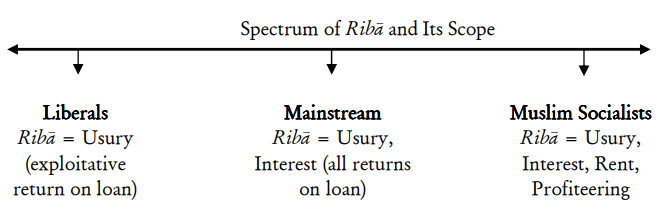
\includegraphics[width=\textwidth]{CourantsIslamContemporain/ImagesCourantsIslamContemporain/Riba.png}



The above differences have left scholars divided on several important questions that demand straightforward answers. Those questions include the following ones:
\begin{itemize}
    \item 
1. Is bank interest prohibited in the light of the Qur'an and the sunnah? If yes, how?
    \item 
2. Whether the Qur'anic term riba includes all kinds of interest rates or it relates only to the excessive interest rates?
    \item 
3. Whether the scope of riba extends to the interest charged and paid on business transactions in the banking system or is restricted to the interest charged on consumption loans only?
    \item 
4. Does Islam allow loan transactions? If yes, how and in what form?
    \item 
5. Is paying interest a lesser evil as compared to charging it?
    \item 
6. Is borrower always \textit{mazlum} (a losing party) in an interest bearing loan transaction?
    \item 
7. Does Islam allow indexation of loans on the grounds of inflation?
    \item 
8. Is credit-sale with higher deferred price as compared to the spot price allowed?
    \item 
9. Does Islam approve of “time value of money,” especially when charging higher deferred price is allowed in a credit sale?
    \item 
10. Are future currency contracts permissible in Islam?
    \item 
11. How and to what extent is salam transaction permissible?
\end{itemize}


These are but a few questions.
\begin{Synthesis}
We show in this paper that whatever confusion prevails among contemporary scholars on this subject is the outcome of following an inadequate methodology for determining the meaning and scope of riba.
\end{Synthesis}
 In fact, this methodology has mystified the nature of riba, which is otherwise clear when viewed from the methodological view point of the eminent Muslim jurists of the past. The mystification is such that not only it results in confusing answers to these questions but it also begets confusing questions. Unfortunately, the confusion has built up to the extent that the Federal Shariat Court of Pakistan has been struggling to come up with a definition of riba. It is in this background that this paper attempts to explain:

(1) the contemporary Islamic economists' methodology of interpreting and classifying riba; (2) why this methodology is wrong and insufficient; (3) the methodology of understanding riba on the pattern of Muslim jurists of the past; (4) that the methodology given by the Muslim jurists is coherent and compact.

The reader will encounter a number of arguments in this paper that are advanced by those who justify bank interest. Since the paper deals with the legal substance and not with the economic merits of arguments, hence we will restrict ourselves to the legal analysis of those arguments and leave aside their economic analysis and rationale, which require an altogether different methodology. Any legal system has three aspects: (1) what: the legal rulings (i.e., ahkam); (2) how: the rules of deriving those legal rulings (i.e., usul al-fiqh); and (3) why: the underlying rationale(s) and wisdom behind the legal rulings (i.e., hikmah)

It is important not to mix these aspects. The present study deals with the first two aspects of the issue of riba. Moreover, the classification of riba discussed in this paper is primarily based on the methodology of Hanafi jurists for ensuring analytical consistency. We presume that a school of law represents an internally coherent system of interpretation and that mixing up the views of the various schools results in inconsistencies.7 However, views of the other schools have been briefly mentioned in the footnotes wherever required. Finally, the paper does not attempt to show that the Hanafi jurists' approach is superior to all others, rather it explains that the classical jurists' approach (whether Hanafi, Maliki, Shafi‘i or Hanbali) to understanding riba is superior to that of the modern scholars. The methodology of these jurists share several common results that are important in order to answer the above questions.

Following section outlines the method adopted by modern Muslim scholars and economists. The next section discusses problems in this methodology and develops the skeleton for the methodology that is then applied in the coming section, which details out the general rules of riba alongside their resulting implications. The last section concludes the paper by giving a comprehensive definition of riba based on discussions in sections three and four.


\newpage
\subsection{Outline of the Mystifying Methodology}

Imran Ahsan Khan Nyazee\sn{\href{https://en.wikipedia.org/wiki/Imran_Ahsan_Khan_Nyazee}{Pakistan} Nyazee's academic career was inspired by the work of Abdur Rahim. Nyazee argues firstly, that due to its unique set of principles of interpretation, each school of Islamic law represents a theory of law unto itself. Secondly, he points out that Istiḥsān cannot be understood without understanding of the workings of qiyās. It is, therefore, difficult to accept that there was no system of interpretation before al-Shāfi‘ī's time. Thirdly, he concludes that the uṣūl al-fiqh never existed. Furthermore, Nyazee describes beyond the individual fikh of each school of law, another theory of interpretation called maqāṣid al-sharī‘ah (theory for the purpose of the sharī‘ah) which was developed by al-Ghazālī. Nyazee has written and self-published on a number of aspects of Islamic law. He agrees with most Muslim scholars that strictly speaking, selling money (taking interest) is prohibited, according to Islamic law. Some point out a difference between the treatment of riba in the Qur'an versus the Sunnah but Nyazee the two approaches are actually one and the same.Nyazee also proposes that all loans (except those of a charitable nature without a fixed period of repayment) and therefore all banking is prohibited and unIslamic. Nyazee is equally intolerant of murabaha, the Islamic system of business where in-put costs and mark-ups are made transparent between vendor and buyer. He argues riba will inevitably enter such transactions.[10] He extends the prohibition to the creation of wealth on the basis of debt and the fractional reserve banking system. These elements along with zakat (the system of alms-giving) he says, are the differences between Islam and capitalism. He advocates the use of the gold and silver dinars and dirhams as the currency of the Muslim community. Nyazee would also prohibit the corporation or 'legal personality' under Islamic law.} explains that the methodology adopted by modern scholars for determining the meaning of riba is the same, though they disagree in their conclusion regarding whether or not bank interest is riba.8 The fundamental problem of their methodology lies in overlooking the inherent link between the Qur'an and sunnah. This methodology of interpreting riba was initiated by Muhammad Rashid Rida (d. 1935) \sn{voir p. \pageref{Theol:Rida} Frère musulman pas le voyage en Europe. Plue el manar un commentaire coranique, sensé être l'héritage d'abdu}, which goes as follows:9

\paragraph{Lecture de Rida El Manar}
Riba is classified into two categories, riba of the Qur'an (also equated with riba 'l-nasi'ah, i.e., interest on loan transaction) and riba of hadith (equated with riba 'l-fadl, i.e., interest on exchange transaction).

Rida begins with literal meaning of the word riba (excess) and then traces some riba-based transactions practiced by Arabs during the time of Prophet (peace be on him). Rida, relying on some commentators of the Qur'an, asserts that the Qur'anic verse regarding riba deals with a specific practice of Arabs known as credit-sale where the payment of price is deferred to a future period while delivery of goods takes place on spot. Because a seller is allowed to charge whatever price he wants in a sale transaction, no riba is involved in the original price negotiated between the two parties-any excess in future price becomes part of the price. However, they used to increase the price excessively whenever the debtor would be unable to settle his debt obligations at the end of payment period. The debtor was given the option, “Will you pay the debt or increase the amount in lieu of delay?”

For Rida, it was this excessive rate (doubling and multiplying) of interest in debt-based transactions added to the original sum at the end of payment period which was prohibited by the Qur'an (he called it riba 'l-jahiliyyah).10 From this, he concluded that the bank interest is not the same riba that was deemed impermissible by the Qur'an because (a) it is neither doubling and redoubling of rates (b) nor the excess is stipulated in the initial period of the banking transaction-he assumes that the initially added interest is part of the principal or original sum just like the original sum in case of credit-sale. 
\begin{Synthesis}
Hence, for Rida, only compound interest is prohibited.
\end{Synthesis} 

Other scholars, supporting Rida's view, added that business loans were not common among Arabs as theirs was a subsistence economy; loans were largely taken by poor people for consumption purposes on interest and whenever they were unable to repay them at due time, excessive interests were added to the original sum. Hence, it was this type of interest that was declared prohibited by the Qur'an and it has nothing to do with the modern commercial loans, \textbf{which are mutually beneficial for both parties.}11

Having ascribed this meaning to the Qur'anic word riba on the basis of some historical traces, Rida then explains the form of riba declared impermissible in the sunnah as a distinct prohibition from that of the Qur'an.
\begin{Def}[Riba] Usure, profit ou gain réalisé sur un prêt.
\end{Def}

\begin{Def}
[Riba al-buyu] : Usure. Opération de vente dans laquelle une matière première est échangée contre la même matière première mais en quantité différente et la livraison d’une des matières premières est postposée. Pour éviter le riba al-buyu, les matières premières échangées par les deux parties devraient être en quantités égales et l’échange devrait être instantané. Riba al-buyua a été condamné par le Prophète Muhammad afin d’éviter que le riba (intérêt) n’affecte insidieusement l’économie.
\end{Def}
\begin{Def}[Riba al-duyun] : Usure d’une dette.
\end{Def}
 
\begin{Def}[Riba al-fadl] : La différence de quantité entre deux biens échangés et comportant du riba.
\end{Def}
\begin{Def}[Riba al-nasiah] : La différence de paiement liée au report de deux biens comportant du riba
\end{Def}\mn{cf Glossaire des termes financiers  Islamiques \href{https://www.cairn.info/la-banque-et-la-finance-islamiques--9782804167042.htm}{Banque et finance islamique} } He calls it \textit{riba 'l-fadl} which emerges in the exchange of two counter values of the same or different species and hence also called \textit{riba 'l-buyu‘}.12 The position of Rida, which may be termed as minority view, is summarised in figure 2.


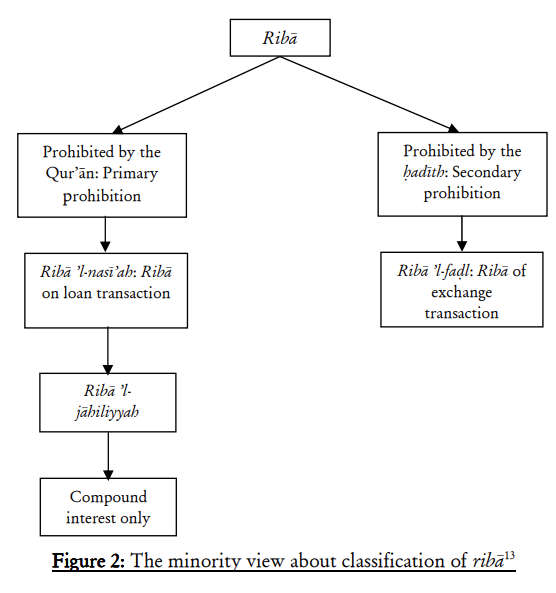
\includegraphics[width=\textwidth]{CourantsIslamContemporain/ImagesCourantsIslamContemporain/RibaRida.png}

Thus, Rida dichotomised the two concepts of riba, one attributed to the Qur'an and another to the sunnah. He finally declared the first one as real or explicit riba while latter as lighter or implicit riba.
\textbf{
Though the majority of contemporary scholars did not agree with the conclusion drawn by Rida about legitimacy of bank interest, however they adopted his methodology of classifying riba. The only difference in their opinion is that riba of the Qur'an includes all rates of return on loan and it is not merely restricted to the compound interest of jahiliyyah}\sn{la période pre islamique}


To them, business loans were a part of Arab's economy and any contractual return to lender is unfair because this is tantamount to refusing to share business risk with the borrower. We can depict their views in figure three.
\begin{Synthesis}
On a donc un nouveau problème, le pret commercial lié avec l'industrie et face à ce nouveau problème, une lecture de Rida qui est assez positive (Riba = Excess) mais qui note une différence entre Coran et Sunna) et fait une distinction entre les deux, reprises ensuite par les autres légistes, mais en repartant d'une lecture stricte du Riba comme intérêt. Il conveint d'articulier Coran et Sunna de façon non parallèle mais l'un par l'autre.
Il convient de montrer l'évolution du prêt commercial au XIX
\end{Synthesis}
Because the sunnah is not linked with the Qur'an in this methodology, both the minority and majority Muslim economists have struggled to explain as to why someone would engage in exchange transactions of the forms mentioned in hadith. Some opined that these transactions are declared impermissible because they may open the path for the “real riba” (i.e., riba of the Qur'an).


14 Others assumed that it was meant to discourage the practice of barter exchange and promote market exchange through a medium of exchange.15 Yet another view argues that it eliminates the possibility of benefiting from asymmetric information of the contracting parties.16 The truth is that none of these explanations makes the point.

2.1. The Nature of Debate within Minority and Majority Schools

The debate that has taken place within the followers of this mystifying methodology on the issue of why or why not bank interest is riba may briefly be summarised here. As explained above, Rida asserted that bank interest was not included in the Qur'anic concept of riba of debt because it was different from the riba that was charged by Arabs on credit-sale transaction by doubling and multiplying the price whenever the debtor was unable to settle his debt at due time and asked for relaxation in payment period.18 Rida explained that the Qur'anic verse “Allah has permitted bay‘ and prohibited riba”19 referred to this riba. To strengthen his case, he argued from the verse: “O Believers! Do not devour riba doubled and multiplied and fear God so that you may prosper.”20

This verse complements the former verse in the sense that what was implicit in the first verse was made explicit in the latter-both verses referred to the practice of doubling and multiplying of interest and none of them forbad the bank interest.

How do the majority of scholars respond to this argument? For example Usmani notes the Qur'anic verse:

O you believers! Fear God and give up riba that remains outstanding if you are true believers. Behold! If you do not obey this commandment, then God declares war against you from Himself and from His Prophet. But, if you repent (from riba), then you are entitled to only your principal amounts. Neither should you inflict harm to others, nor others should do harm to you.21

The argument is based on the emphasised words ‘you are entitled to only your principal amounts (ra's al-mal)'. He infers from these words that the rightful entitlement of lenders is the original sum advanced; he cannot charge any increase whether small or large (doubled and tripled). To him, the verse (3:130) forbids a severe form of riba where interest is multiplied, but it does not restrict riba to this specific form. Hence, bank interest falls within the purview of the Qur'anic verse “Allah has permitted bay‘ and prohibited riba.”22 They are also of the view that charging interest on commercial loans was also practiced by Arabs.23

Does the above analysis of mainstream scholars guarantee the prohibition of bank interest? We are afraid it does not. Their arguments rest on two assumptions:

(1) The verses (2:278-79) address the issue of loan-transaction.

(2) Ra's al-mal (principal amount) can only refer to the original principal advanced in loan.

Both of these assumptions are problematic. Following submissions can be made against them:

(a) If the meaning of the verse is to be determined with reference to historical practices, one can equally claim, just like Rida, that the verse is not about loan transaction but about credit sale. In that case, ra's al-mal is not referring to the principal amount lent; rather, it is the deferred future price of the goods sold. On which legal grounds or facts can this claim be dismissed?

(b) Further, this deferred price might include increase over and above spot price. Hence, the future price could consist of two components: spot price plus some additional profit. The sum of these two would constitute ra's al-mal (principal amount) in this transaction (i.e., principal amount in credit sale (ra's al-mal) = spot price + extra profit)

Whenever a debtor was unable to repay full amount, further multiplied increase was added to this original sum, Rida called it interest. This would increase the due amount to: total amount after increase added due to delay, which is interest in addition to ra's al-mal.

Using this structure, one can then argue that the initially added interest in a loan transaction is equivalent to initially added “extra profit,” which becomes part of ra's al-mal. Therefore, entitlement to the ra's al-mal means entitlement to the simple interest, as claimed by Rida.

(a) The only legal justification for ascertaining that the verse is about loan transaction is based on the words “ra's al-mal” (principal amount). But how can it be settled that ra's al-mal here means ra's al-mal of a loan transaction? This question is important because a number of transactions constitute a component of ra's al-mal. For example, there is ra's al-mal both in mudarabah and musharakah contracts. How to exclude these forms of ra's al-mal from the purview of the Qur'anic verse? If someone says, “This verse is about loan, so ra's al-mal refers to that of loan contract and not of mudarabah and musharakah,” he is clearly arguing in circularity. The argument goes like this:

Q: How do we know that the verse is about loan contract?

A: Because the verse talks about ra's al-mal.

Q: How do we know that ra's al-mal here refers to that of loan?

A: Because the verse is about loan contract!

A circular argument is no argument.

(b) Muslim Socialists could maintain that ra's al-mal means principal amount of all business contracts. Therefore, it is not legitimate to charge any excess over and above principal amount, no matter it is mudarabah, musharakah or ijarah.

Not only that the analysis of mainstream scholars does not necessarily imply the prohibition of bank interest, it leads to a set of unsettling arguments that have left Islamic economists bewildering about some basic issues. For example,

(1) Even if it is agreed that ra's al-mal means principal amount of a loan transaction, does it mean “nominal” amount or the “real” (inflation adjusted) amount? Again, what are the legal grounds to settle this issue? Because there are no clear-cut legal grounds available in this methodology, we see scholars are divided on this subject matter-some allow indexation of loan against inflations while others do not.

(2) What about the question of “time value of money?” This question poses challenge for Islamic economists because they, as a rule, approve the practice of charging higher price in credit-sale and murabahah.

(3) The Lawgiver has allowed salam, what are the legal grounds for not extending this permission to currency salam (future currency contracts)?

Undoubtedly, majority view has addressed these issues, but the answers do not seem to be stemming out of a coherent analytical legal system. This approach is often found mixing up legal analysis with economic analysis. This missing coherent analytical legal system is the root cause of most of the mystification that has prevailed all over. It is an unfortunate state of affairs and it is high time to demystify things.

3. Methodological Assumptions of Premodern Muslim Jurists (Fuqaha') for Understanding Riba

To understand the method used by the eminent premodern Muslim jurists for understanding riba, three methodological issues (MI) need to be clarified. They are explained by Nyazee in detail.24

1) Link between the Qur'an and Sunnah

The methodology adopted by the modern Muslim scholars and economists is misleading because it delinks the Qur'an and sunnah. It assumes that the meaning of riba is different in the Qur'an and sunnah, which is not the case. To explain the nature of error made by both the groups, it should be noted that Muslim jurists (fuqaha') classified riba in the category known as mujmal (unelaborated)25 whose meaning and scope cannot be determined without explanation (bayan) of the Lawgiver (Shari‘). The famous hadith (as given in footnote 1) that explains different usurious transactions actually does not add something to the Qur'anic word riba. Rather, it defines its meaning and scope.

Thus, while to the contemporary scholars the meaning of riba is known independent of hadith and they see hadith as adding some more cases to the Qur'anic concept of riba, the jurists say that hadith is the definition of the term riba used by the Qur'an. Thus, riba 'l-nasi'ah and riba 'l-fadl both are included in the Qur'anic concept of riba.

2) Relationship between Loan and Bay‘ (Exchange)

Loan is also classified as a form of exchange transaction (bay‘)26 by Muslim jurists. The scope of this paper does not allow detailed analysis of this assertion.27 For descriptive purposes, it can be seen that a loan of Rs X is an exchange of Rs X today with Rs X after time deferment (and with Rs X + Y if interest payment of Rs Y is included). Figure 4 depicts this nature of loan transaction by illustrating a loan transaction between Mr. A and B:

3) Skeleton of a Coherent Legal System

A coherent shari‘ah-based legal system consists of a set of general rules, called

‘azimah by the jurists, supplemented by some exemptions to these laws, called rukhsah. In the words of Nyazee, ‘Azimah (lit. determination, resolution) is applied to mean a rule that is applied initially and for itself. Such rules form the backbone of the law. As against this, there may be a rule that goes contrary to the requirements of the initial rule, but is permitted by the law. This rule is considered to be a rukhsah (exemption) from the initial rule.28

This classification of ‘azimah (the higher or first order rules) and rukhsah (the lower or second order rules) is important for several reasons.

First, it explains the order in which the rules have to be applied.

Second, it explains why sometimes two opposing cases may be allowed within a given skeleton of law.

Third, the order of rules implies that an exception cannot be extended using any method of argument, whether analytical or analogical. On the other hand, extension of first order rules is legitimate by these methods. In other words, it is not allowed to build a sub-legal system based on exemptions because otherwise it starts negating the primary provisions and objectives of the law-an exemption from the general rule must remain an exemption.

Fourth, because of the logical hierarchy in the operations of ‘azimah and rukhsah, it is clear that an exemption from a rule cannot be used to nullify or change the shari‘ah status (hukm) of any other case that is derived from the general rules. Alternatively put, an exemption (a lower order rule) cannot prevail over the higher order rules.

Fifth, because all rules and exemptions are derived from nusus (the Qur'an and sunnah), hence the only justifiable exemptions are the ones, which are given in nusus (i.e., stated by the Lawgiver Himself).

We call these nusus the “facts” of the shari‘ah-based legal system in this paper. Given these “legal facts,” the task of a jurist is to derive those general rules (‘azimah) from the facts, which render these facts internally consistent and extendible on the one hand and highlight the exemptions (rukhsah), if any, on the other.29 Finally, the general rules and exemptions generate some implications, called ahkam. This skeleton of a shari‘ah-based legal system is illustrated in Figure 5. We apply this skeleton in this paper to elaborate riba.

The relevant “legal facts” used by premodern Muslim jurists to derive general rules and exemptions are quoted at the relevant places in this article. We are now in a position to take on the issue of derivation of the general rules and the implications from those “facts.”

4. Underlying Rules behind the System of Bay‘ in Jurists' Methodology

Our intention in this paper is to reveal that the apparently large and complicated system of legal injunctions (ahkam) is reducible to a few set of rules derived from fewer legal facts. We propose that a majority of ahkam (legal injunctions or provisions) governing economic transactions (buyu‘) can be derived from three broad rules:

1. Rules of riba mentioned in the sunnah. This is not a single rule, rather a set of rules as explained below.

2. Rule about the sale of goods not possessed by a person.

3. Rule about exemption that an exemption is to be treated as exemption.

Before explaining these rules, we first explain the context of the Qur'anic verses that underlies the jurists' methodology of riba to clarify the misconception that the relevant verses of Surat al-Baqarah are about loan transaction and not exchange (bay‘).

4.1. The Context of the Verses of Surat al-Baqarah

The Qur'an states that the disbelievers said, “Verily, bay‘ (sale) is just like riba.” In response to this, it was said, “Allah has permitted bay‘ and prohibited riba.” To understand why the disbelievers said this, consider these three transactions:

(a) A gives B 100 grams of gold in exchange of 110 grams of gold to be paid after one year. This is primarily a sale contract as explained previously (i.e., exchange of 100 grams gold with 110 grams gold with time lag) and involves riba (how, this will be explained in the next section but take it for granted for the moment).

(b) A asks B for 100 grams of gold in exchange of, say, 500 kg wheat at spot. This is a legitimate regular sale contract.

(c) A demands from B 110 grams of gold in exchange of 500 kg wheat for payment of price after one year: this is credit sale contract with higher deferred price as compared to spot price and is also legitimate (this is explained in section 4.3).

The credit sale was a common practice among Arabs and, therefore, they were confused as to why the transaction (a) is impermissible and (c) is permissible while the two are quite similar in nature (i.e., both are credit sales and both involve access payment). In (a), 10 grams of additional gold are paid as counter-value for 100 grams of gold for a delay of one year and similarly 10 grams of gold are paid for a delay of one year in transaction (c). It is for this reason that disbelievers said, “Verily sale is just like riba!” That is, transaction (c) (i.e., the credit sale) is similar to the transaction (a). The technical reason for allowing transaction (c) and forbidding (a) is the similarity of genus which is explained by the sunnah. This is explained in the next sections in detail, but the important point to note here is that the assumption that the Qur'anic term riba is not about sale contract, rather it is about debt, is not implied by these verses.

Thus, the verse says that Allah has approved all forms of buyu‘ (exchange transactions) except those which involve riba.30 The natural question then arises: what is this thing called riba? Has the Qur'an given any definitive description of riba?

One may make one of the two assumptions here. First, the concept of riba was largely a sort of common knowledge for everyone and, hence, it required no legal description by the Qur'an. That common knowledge is traceable by an examination of historical record of Arabs which provides sufficient legal foundations for determining the meaning of riba. As far as the details of riba in the sunnah are concerned, they were additions over and above to that common knowledge of riba and most of these additions were unknown to the Arabs. The liberals and mainstream scholars share this assumption and we believe that this assumption constitutes what we called the “mystifying methodology.”

Second, some forms of riba may be or actually known to the Arabs but these do not set the legal standard against which the Qur'anic concept of riba is to be determined. As it is a legal term, its meaning has to be sought from the Lawgiver. In technical sense, the jurists call it mujmal (unelaborated) for which elaboration (bayan) is sought from the Lawgiver. This elaboration of the legal meaning of the Qur'anic term riba is given by the sunnah. After this elaboration by the Lawgiver, its meaning is determined definitively and it becomes mufassar (elaborated). This is the methodological assumption that the jurists use not only for defining riba but also for other legal terms of the Qur'an, such as salah, zakah, and so on.31 Thus, according to this second assumption, the practices and concepts of Arabs may be referred by the Qur'anic concept riba but it is not the benchmark against which we assign legal meaning to the Qur'anic terms.

For example, the Arabs had some concepts about how to offer salah (prayer), but this information does not define the legal meaning of the Qur'anic term salah nor is this concept limited to this information set. Similar is the case with riba. The Arabs might have been aware of some forms and practices of riba but that does not constitute the legal definition of riba. When the jurists classify a term as mujmal, they mean that this term is a technical legal term and its meaning should be determined with reference to the words of Lawgiver Himself, neither by the linguistics (dictionary) nor by the historically known social concepts and practices that hover around that technical term. It should be emphasised here that considering riba as mujmal does not mean that the Arabs did not know the meaning of this word at all. Nor does it mean that the pre-Islam Arabs did not identify certain transactions as riba-in fact they did and the jurists did consider it part of riba.32

It only means that the meaning of riba in Islamic law is not limited to, and is not based on its usage in the pre-Islam Arabia. The Qur'an and the sunnah added several shades of meaning to this concept. That is why, it became a “technical term” of Islamic law. Hence, its meaning and scope cannot be determined by its dictionary meaning or its practice and understanding by the pre-Islam Arabs. Rather, it must be determined by the Qur'an and the sunnah, like any other legal term such as salah and zakah. Just as we cannot classify concept salah as salah of the Qur'an and salah of hadith, similarly we cannot dichotomise riba. Once it is established that the meaning of riba must not be gathered from pre-Islamic usage and practices but from the Qur'an and the sunnah, the next question is: how to explain the various usages of riba in the Qur'an and the sunnah? The answer, as per the well-established methodology of the jurists, is to consider the sunnah as the elaboration of the mujmal verses of the Qur'an.

This methodology is employed by the jurists for determining the meaning and scope of salah and zakah as well as riba. Let's follow through the path of righteous ones here and have its blessings.

4.2. General Rules of Riba When Transacted Species are Same

Keeping these in mind, one has to understand the classification of riba in the system of Muslim jurists. Because the sunnah defines riba, note the words of hadith,

When you exchange gold for gold, silver for silver, wheat for wheat, rice for rice, dates for dates, and barely for barely, then exchange like for like (in equal measure) and exchange them hand to hand (at spot), else it will be riba.33

To understand what it says, consider these transactions:

1) exchange of 1 gram gold for 1 gram gold on spot;

2) exchange of 1 gram gold for 2 grams gold on spot;

3) exchange of 1 gram gold at spot for 1 gram gold with delay;

4) exchange of 1 gram gold at spot for 2 grams gold with delay.34

As per the hadith, the first transaction is allowed; the second one is disallowed because it involves excess in measurement/quantity (called riba 'l-fadl); the third transaction is also impermissible because the hadith says that the exchange of homogeneous goods is allowed in equal measurement provided it is on spot; therefore, this transaction involves the riba 'l-nasi'ah (i.e., riba of delaying); finally, the fourth transaction involves both types of riba. These transactions provide two guiding rules (R):

R 1.1) Goods of the same species cannot be exchanged immediately unless their measurement (in terms of weight or volume) is same.

R 1.2) Goods of the same species cannot be exchanged with time lag, even with same measurement.

4.2.1. Implications

Five important implications (I) should be noted.

I. 1) Impermissibility of Market for Loanable Funds

Application of rule 1.2 gives the important implication that loan, with or without interest, is prohibited in Islam because, as explained above, a loan is an exchange of homogeneous goods with time lag. Does it mean that loaning is not allowed in Islam under any circumstances? Of course, this implication of the general rule is at odd with a number of legal facts (nusus), which promise reward for offering loan to the needy ones. How to reconcile these apparently contradictory legal facts now? This is where the concept of rukhsah (exemption) is activated by the jurists. Though loaning is against the general rule (‘azimah) given by the Lawgiver, yet it is allowed by Him as an exemption from this prohibition if it takes the form of benevolent giving (tabarru‘ or sadaqah).35 Loan is classified as tabarru‘ if:

(a) it is out of the intention of benevolence to the other person (i.e., the lender consciously bestows upon the borrower the benefits associated with his asset);36

(b) no increase in its value is stipulated, else it would cease to be benevolent and would involve riba 'l-fadl; and

(c) no contractual time limit is stipulated, the lender can ask for his asset anytime he wants.37 Stipulating (legal) time constraint in loaning activity makes it a business transaction as per the application of general rules of shari‘ah and, hence, unlawful because in that case it is simply the exchange of homogeneous goods with time delay, which is not allowed, whether or not interest factor is included. Moreover, making the time period binding would imply that the lender is forced to do, or to continue with, an act of charity. This is against the very nature of charity.

In short, this principle implies that Islamic law does not permit the “market for loanable funds.” It sees loaning as an act of benevolence, especially in favour of one's relatives.38 Stated alternatively, loan is purely a social transaction (a means of tying and strengthening social bonds) in Islam and not a business. It was in this social transaction capacity that the institution of loan prevailed for thousands of centuries not only in Muslim societies but also in other civilisations of the world until the emergence of capitalism in the fifteenth century.39 Note that this important result (impermissibility of the market for loanable funds) does not follow directly from the classification of modern scholars of Islamic economics, as the majority view allows interest-free non-benevolent loans as a general rule and not as an exemption.

This implication answers one of the important arguments in favour of bank interest given by some economists. The argument says that interest should be allowed in shari‘ah because interest is the price of capital and without interest the market for loanable funds cannot be equilibrated. Because we are not dealing with the economic merit of arguments in this paper, we ignore its economic substance and comment on its legal merit only. It is clear from the above implication now that this argument has no shari‘ah basis because shari‘ah does not allow market for loanable funds to begin with, let alone equilibrating it from shari‘ah perspective.

Before moving on to the next implication, the important implication and exemption regarding loan transactions be noted:

I 1.1) A loan transaction is prohibited, whether or not interest factor is added to it.

I 1.2) A benevolent interest-free loan is recommended as an exemption to the general rules of riba by the Lawgiver.

I. 2) Impermissibility of Bank Interest

All forms of bank interest, whether simple or compound, are prohibited by Islam as per Rules 1.1 and 1.2. Similarly, the fact whether loan is made for business or consumption purposes makes no difference to this result. There remains no confusion about these conclusions if the shari‘ah rules are applied with consistency. In fact, the practice of charging interest by the bank includes both kinds of riba and it, therefore, may be stated that it is the most comprehensive form of riba! This can be verified from the figure 6, which depicts detailed structure of riba-based transactions in case of homogenous goods (leaves aside heterogeneous goods for the moment).

I. 3) False Dichotomy between “Giving and Taking” Riba

The recipient of riba is not always the lending party as is usually perceived. It can be seen from above examples that in case of transaction (2) the lender is the beneficiary of riba, but in transaction (3) riba is received by the borrower, and finally both are its recipients in transaction (4). Hence, opinions such as “taking riba is a greater evil than giving it and, hence, paying interest to the bank is a lesser evil” are based on the fallacious assumption that it is only the bank that receives interest in a typical interest-bearing loan transaction. This wrong assumption is the outcome of using the wrong methodology outlined in section two.40

I. 4) Mutually Beneficial Riba is Prohibited

The view that bank interest realised in transaction (4) is or should be permitted (as claimed by liberal Muslim scholars) is implicitly based on the assumption that “two wrongs make one right”-that is, it assumes that mutually enjoyed riba of the lender and borrower can make this transaction acceptable while the matter of fact is that each of them is separately prohibited to begin with.

I. 5) Irrelevance of Time Value of Money

Following the wrong methodology has resulted in another confusing argument that the bank interest should be allowed because of “time value of money.” This argument is based on the presumption that Rs. 1 today is worthier than Rs. 1 tomorrow. Why? Economists believe that this is due to the subjective time preferences of an individual. A rational (i.e., self-interested utility maximising) economic agent is said to have positive time preferences in the sense that consumption today is preferred to consumption tomorrow because the latter is uncertain, which makes him impatient, thus he wants to have it today than tomorrow.

Another reason for having this positive time preference emerges from the institutional arrangements: if I have the option of earning some interest (say Rs. Y) on Rs. 1 by putting it in a bank account today, why should I lend it to someone for free? Putting Rs. 1 in a bank account will make it “Rs. 1 + Rs. Y” for sure (assuming away bank insolvency), say, after one year while lending it to someone will leave it worth Rs. 1. Hence, Rs. Y (which may be expressed in percentage) is the price that should be paid to the lender for a loan of one year, else it would be unfair with him. This argument is more of economic than legal in its substance, however, some comments can be made here to evaluate its legal substance in the light of preceding discussion.

The relevant part of the proposed argument is the second one (the institutional arrangement) because the first one is merely a subjective feeling, which may differ from person to person (as a matter of fact, not everyone prefers to consume more today than tomorrow). The argument presumes that there exists and should exist a well-established legally functional market for loan, which coordinates interest-based loan transactions. But just recall “I.1” that Islam does not approve of the market for loan to begin with. Eliminate this institution of market for loan, and the argument disappears. The point is that the concept of “time value of money” conceived in this economic sense is alien to the discussion of riba. Its validity presumes that there exists a legal institutional market for loanable funds where money is growing continually and, therefore, an individual always has the option of putting his money in that market.

Not only that this assumption is invalid from the point of general rules of shari‘ah as explained, it is also in contradiction with the ontological structure of the universe and economic facts.

The above is not the only format of this argument, it is phrased in some other shades as well. For example, it is stated that money could buy benefits and had the lender not lent it he could have benefitted himself. This implies that lending is an act of sacrificing the benefits associated with money. Therefore, the lender should be compensated for this sacrifice and interest payment is exactly that reward. This reward makes sense given that the borrower takes benefit out of money. The argument is valid to the point that money is beneficial to the lender and that if he makes the choice of not lending it, he can benefit from it. Moreover, it is also true that the borrower enjoys the benefits associated with the money. None of these facts is denied by the shari‘ah rules. But these facts alone cannot formulate the required case for this argument; it requires a moral statement in its premise to derive the desired conclusion.

To see this, note that the argument does not end here, after quoting these facts it then makes a moral assertion: “it is morally (and hence legally) right if money is lent for reciprocal benefits.” Addition of this moral statement is necessary for validating the conclusion that “interest is the just reward for lending.” But this moral assumption contradicts the general rules of the shari‘ah, which are laid down above. Seeking reciprocity in loan is exactly what that changes its status from tabarru‘ to loan as a business transaction and, hence, it becomes nothing but riba. The argument here is quite straightforward:

The owner of money is granted the right of benefitting from his money by shari‘ah rules; he is given the option of making a conscious choice of transferring the benefits associated with his money to another person as an exception to the general rules by the shari‘ah, but there is neither any general rule nor any exemption from the Lawgiver that assigns him the right of lending money in the name of the so-called “mutual benefits” (refer to I. 4 above). Legally speaking, this involves both riba 'l-fadl (because the homogeneous goods are exchanged at different rates) and riba 'l-nasi'ah (because time stipulation is invoked-the lender asks for the excess of measurement for parting with the benefits of his money for a specified time).

Another variant of this argument comes with the heading of “effects of inflation on money.” We deal with it in the next section.

4.3. General Rules of Riba when Transacted Species are Different

What about the exchange of heterogeneous goods? The last words of the hadith are as follows: “If these species differ, then exchange as you like as long as it is from hands to hand.”

They give an immediate rule:

R 1.3) Goods of the different species can be exchanged with difference in measurement.

This rule says that such goods can be exchanged at different rates as far as measurement is concerned. In other words, riba 'l-fadl does not apply in case of heterogeneous goods. Is riba 'l-nasi'ah (prohibition of time delay in payment) also not applicable in this case? Apparently, it seems that it is not because of the words of hadith, “exchange should be on spot.” This has an odd implication that credit sale (sale of goods against money where payment is deferred to future time period) is not permissible under the shari‘ah rules. This is so because credit-sale is an exchange of heterogeneous goods with time lag. But the legal facts reveal that the Lawgiver has allowed credit-sale.41 How to explain this? Is credit sale also an exemption to the general rule, like a loan transaction? The answer is: “No, it falls within the general rules.”

To see how credit-sale is permissible within general rules, one needs to dig deep into the issue of the underlying cause (‘illah) that the Muslim jurists derived from the sunnah to understand the system of riba. The relevant question facing jurists was: Is prohibition of riba restricted only to the six goods named in the hadith or is it extendible to other goods? The answer of the jurists is, yes, it is extendible and for this extension they derived the underlying cause due to which riba was declared prohibited by the Lawgiver. Keeping aside the technical details and arguments, it should be noted that some of the goods are measured in terms of weight while others are measured in terms of volume. In the hadith under discussion, gold and silver were weighable while the other four items were volumeable at the time of Prophet (peace be on him).42 Based on this classification, the jurists derived two further rules:

R 1.4) when species are different but their method of estimation is the same (such as gold vs silver or wheat vs rice), unequal quantities can be exchanged, provided that the exchange is immediate;

R 1.5) when species are different and their method of estimation is also different (such as gold vs wheat), unequal quantities can be exchanged with time delay.43

Thus, the credit sale is allowed due to the application of Rule 1.5. To see this, consider these combinations of transactions:

1) Exchange of 1 gram gold at spot for 2 gram silver on spot (method of estimation same)

2) Exchange of 1 gram gold at spot for 2 gram silver in future (method of estimation same)

3) Exchange of 2 kg wheat at spot for 1 gram gold/silver on spot (method of estimation different)

4) Exchange of 2 kg wheat at spot for 1 gram gold/silver in future (method of estimation different)

The first transaction is allowed but the second is not because when species are measured by same method (i.e., “weight” in this case), then difference in the measurement (fadl) is allowed but deferment (nasi'ah) is not permissible. The third and the fourth transactions are allowed because here not only the transacted species are different but also their method of measurement (one was measured in “weight” while the other in “volume”).

In short, when both of the similarity factors (i.e., species and method of measurement) are found, then both fadl (excess of measurement) as well as nasi'ah (excess of time delay or time deferment) are prohibited. When similarity of measurement is found alone, then fadl is allowed but nasi'ah is prohibited. Finally, when none is found, both fadl and nasi'ah are allowed. Figure 7 depicts all of these rules completely (discussion about the last layer of boxes on the right-hand side of this figure is coming next).

The preceding discussion shows that the hadith explaining the nature of riba was not about the actual practices of Arabs that begged some economic explanations with which Muslim scholars have been struggling. Rather, it stipulated the rules of exchange. It says, “If at all you make exchange transactions, here are the governing rules.” Thus, all transactions that correspond to these general rules are allowed while those in contradiction with them are prohibited (however, some are exempted by the Lawgiver).

4.3.1. Implications

Following implications are derived from the above rules. It is important to note that the first two transactions mentioned in sub-section 4.2 belong to the case when method of estimation of the heterogeneous goods is same while the latter two cover the cases when their method of estimation is different.

I. 6) Placement of Regular and Credit-Sale

Transaction (3) is categorised as regular sale transaction (usually termed bay‘) by the jurists. On the other hand, transaction (4) covers credit sale, which may take two forms: with or without extra profit margin as compared to the spot sale. Because both measurement as well as payment time differential are allowed in this case, hence credit sale of both forms is allowed.

I. 7) Placement of Currency Exchange

The remaining two boxes are relating to the exchange of currencies (termed as bay‘ al-sarf by the jurists). A detailed description of these requires an appreciation of some more technical classifications44 made by the Muslim jurists. However, they are beyond the scope of this paper. Suffice to say that the jurists divided all tradeable species into two: (a) currency items, which are used as means of exchange; they included gold and silver (though other goods may also be treated as currency in this system) and (b) non-currency items, (goods that are exchanged, and are not medium of exchange). They roughly included all but gold and silver.45 Given this division, the jurists broadly mention four types of transactions (buyu‘):

(1) Non-currency item in exchange of non-currency item-called barter exchange.

(2) Spot or delayed currency (say gold) in exchange of spot non-currency (say wheat) item.

(a) If both of them (gold and wheat) are exchanged on spot, it is called regular sale of goods, and

(b) if the currency price (gold) is delayed, this is called credit sale.

(3) Delayed non-currency item (say rice) in exchange of spot currency item (say gold). Here, the price of the good is paid on spot while its delivery is delayed. This is called bay‘ al-salam (advance payment) by the jurists.

(4) One currency (gold) in exchange of another currency (silver)-known as bay‘ al-sarf.

Rules regarding the first two have been discussed above. Here, we have to make some submissions regarding this fourth type of transaction. Because this transaction comes under the umbrella of “different species with same method of measurement,” it is clear from figure 7 that the excess of measurement is allowed in this transaction while time deferment is not. This gives two further rules under rule (1.4):

1.4a) If different currency items (such as gold and silver) are exchanged, then it is allowed to exchange them at any rate;

1.4b) if different currency items (such as gold and silver) are exchanged, then it is not allowed to exchange them with time deferment.

If it is accepted that modern currencies are just substitutes of gold and silver, then two further important results emerge from this discussion:

I 7.1) Future Currency Contracts are Prohibited

Rules (1.4a) and (1.4b) imply that the spot currency transactions are allowed while their future contracts (known as currency salam in Islamic finance literature) are prohibited in Islam as they come under the purview of riba 'l-nasi'ah.

I 7.2) Indexing of Loans is Prohibited

Indexing the value of the currency loans against some underlying assets (say gold) on the ground of inflationary pressures is not allowed. It is often argued that since the value of currency decreases over time due to the presence of inflation, hence an extra-payment equal to the rate of inflation, over and above the original sum given in loan, should be allowed in favour of the lender to keep his purchasing power. Again, because the economic merit of this argument is beyond the scope of discussion in this paper, we restrict only to its legal merit. If it is accepted that one rupee is legally nothing but equivalent of 1 unit of gold or silver (whatever that unit be), then Rules 1.1 and 1.2 (governing the loaning contract in gold or silver currencies) should automatically become operational.

Those rules imply that (a) loaning in the form of currency item is allowed if and only if equal measurement (whatever the unit of measurement) is returned; else it would be riba 'l-fadl; and (b) it is a loan made out of benevolence and not business intention (having time stipulation); else it would be riba 'l-nasi'ah. Hence, adding an extra amount to loan transaction in the name of “indexation” is but both, riba 'l-fadl (because of the excess of measurement) and riba 'l-nasi'ah (because the increase is time bound). 46 Again, let simplicity and sanity prevail.

I. 8) Placement of Salam

To see how the jurists accommodated salam in this scheme, note that there is nothing in the set of rules 1 (from 1.1. to 1.5) which forbids it. However, according to rule 2 (given at the start of this section), selling what one does not possess is not permissible and this is exactly what a salam transaction involves. Thus, a salam transaction should not be allowed as per the general rules of shari‘ah. We are once again faced with the same issue: salam is permitted in the “legal facts;” how and where to place it in the legal skeleton of the shari‘ah? Is there another general rule, which governs its permission as we saw in case of credit sale or is it an exemption from the general rule just like loan? The jurists' answer is the following: Salam is permitted as rukhsah-exemption from the general rules-by the Lawgiver.47

Because it is an exception, as per rule 3, it would be allowed only as “one of its kind” (sui generis) and cannot be used as justificatory mode for deriving more comparable transaction forms (e.g., currency salam). An exception to the general rule remains exception and does not turn into a rule for other cases because then it ceases to be an exception and creates a situation of self-contradictory general rules, which is not acceptable in any legal system. Thus, salam transaction is allowed as an exception for those transactions where (a) a currency item is exchanged against a non-currency item and (b) non-currency item is deferred while the currency-item has been paid at spot.48 This is what the exception is all about; one cannot extend this exception to the transaction types where currency items are exchanged with each other because that would violate condition (a) of the exception case.49

Figure 8 shows a map of interplay among legal facts (nusus), general rules, exemptions, and the derived implications related to riba and bay‘ that are discussed in this paper. This diagram shows that a rather complex looking system of ahkam (implications) showing up at the ending layer boxes of figure 8 emerge out of a set of general rules, which are derived to make underlying legal facts compatible with each other.

5. Conclusion: The Definition of Riba

We conclude this paper by elaborating a comprehensive definition of riba that can be inferred from the discussions in this paper. Let's quote it from al-Sarakhsi:50
\begin{Synthesis}
Riba in its literal meaning is excess... and in the technical sense (in the shari‘ah), riba is the stipulated excess without a counter-value in bay‘ (sale).51
\end{Synthesis}


Let's explain it noting several points about this definition:

(1) Muslim jurists do not introduce the word loan in the definition of riba because they categorise loan transaction under exchange (bay‘). Not appreciating this point resulted in the misconception that since the fiqh conception of riba does not deal with the subject of bank loans, it needs to be inferred directly from the Qur'an.

(2) Riba is excess, either in the form of quantity (qadr) or in the form of benefits of delay (nasa'). The first is called riba 'l-fadl while the latter is called riba 'l-nasi'ah.

(3) This excess is without any counter-value permitted by the shari‘ah. Thus, the excess of quantity paid in lieu of time delay in case of interest-bearing loan is not allowed because these two cannot be the legitimate counter-values (see I. 4).52 For a substance to be counted as counter-value, it must be recognised by the general rules of the shari‘ah to begin with.53

(4) The excess is stipulated in exchange. If the excess is granted voluntarily, it would not be riba.

We started off with specific questions in the introduction. The appendix lists down the answers to these questions in the light of the above definition of riba. It can be seen that once the discussion about riba is placed on the right track, right and clear cut answers start emerging automatically.

Appendix: Questions and their Answers that Follow from the above Analysis

Notes

1 For detailed arguments of this position, see Abu 'l-A‘la Maududi, Sud (Lahore: Islamic Publications, 2000), 110-12; M. Umer Chapra, “The Nature of Riba in Islam,” Hamdard Islamicus 7, no. 1 (1984): 3-24; Muhammad Shafi‘, Mas'alah-i Sud (Karachi: Idarat al-Ma‘arif, 1996), 43-47; Muhammad Ayub, “What is Riba? A Rejoinder” Journal of Islamic Banking and Finance 13, no. 1 (1996): 7-24; Muhammad Taqi Usmani, The Historic Judgment on Interest Delivered in the Supreme Court of Pakistan (Karachi: Idarat al-Ma‘arif, 1999), 12-16; Mohammad Nejatullah Siddiqi, Riba, Bank Interest and the Rationale of Its Prohibition (Jeddah: Islamic Research and Training Institute, 2004), 45-48; and Mahmoud A. El-Gamal, Islamic Finance: Law, Economics, and Practice (Cambridge: Cambridge University Press, 2006), 46-52. Within this category, there are further two approaches.

One approach that represents traditional ‘ulama' emphasises the resurgence of only those business contracts that were approved by the early Muslim jurists. It proposes profit-and-loss sharing (PLS) as an ideal alternative to riba. Though it does not deny the permissibility of other than PLS-based financing instruments such as murabahah and ijarah, yet it affirms that equity-based financing method is the primary means of achieving desirable economic objectives. The second approach is pragmatic one. It justifies a more liberal and flexible stance on structuring shari‘ah-compatible transaction forms that looks for financial engineering to meet all demands of modern banking customer.

2 Muhammad Rashid Rida (d. 1935) was among the foremost proponents of this theory. See his al-Riba wa 'l-Mu‘amalat fi 'l-Islam (Cairo: Dar al-Manar, 2007). Also see Sayyid Yaqub Shah, “Islam and Productive Credit,” The Islamic Review 47, no. 3 (1959): 34-37; Fazlur Rahman, “Riba and Interest,” Islamic Studies 3, no. 1 (1964): 1-43; Timur Kuran, “On the Notion of Economic Justice in Contemporary Islamic Thought,” International Journal of Middle East Studies 21, no. 2 (1989): 171-91; Izzud-Din Pal, “Pakistan and the Question of Riba,” Middle Eastern Studies 30, no. 1 (1994): 64-78; and ‘Abd al-Karim Athari, Sud Kiya Hay? (Mandi Baha' al-Din: Anjuman-i Isha‘at-i Islam, 2008), 8-12 3 Constant J. Mews and Ibrahim Abraham, “Usury and Just Compensation: Religious and Financial Ethics in Historical Perspective,” Journal of Business Ethics 72, no. 1 (2007): 1-15.

4 See Ghulam Ahmad Parvaiz, Nizam-i Rububiyyat (Lahore: Idara-i Tulu‘-i Islam, 1978).

5 Rafi‘ Allah Shihab, Kirayah-i Makanat ki Shar‘i Haithiyyat (Lahore: Kitab Ghar, 1981).

6 Ziaul Haque, “The Nature and Significance of the Midieval and Modern Interpretations of Riba,” The Pakistan Development Review 32, no. 4 (1993): 933-46.

7 For details, see Imran Ahsan Khan Nyazee, Theories of Islamic Law: The Methodology of Ijtihad (Islamabad: Islamic Research Institute, 1994), 9-12.

8 Nyazee, The Concept of Riba and Islamic Banking (Islamabad: Institute of Advanced Legal Studies, 1995), 11-19. Imran Ahsan Khan Nyazee (b. 1945) is a well-known scholar and a prolific writer on the subject of Islamic law and is a former Professor of law in International Islamic University, Islamabad. His major works include Theories of Islamic Law; Islamic Jurisprudence; Islamic Law of Business Organization; and The Concept of Riba and Islamic Banking. He also translated some of the classical texts on Islamic law and jurisprudence, including: Hidayah of Marghinani; Bidayat al-Mujtahid of Ibn Rushd; Amwal of Abu ‘Ubayd; and first two volumes of Muwafaqat of Shatibi.

9 Rida, al-Riba wa 'l-Mu‘amalat fi 'l-Islam, 69ff.

10 Period before the advent of the Prophet (peace be on him) is referred to as jahiliyyah (i.e., the period of uncivilised state of affairs).

11 Fazlur Rahman, “Riba and Interest,” 7-8.

12 In this regard, a hadith reads, “The Prophet said, ‘While exchanging gold for gold, silver for silver, wheat for wheat, barley for barley, dates for dates, and salt for salt, exchange like for like, in equal measure, and exchange from hand to hand. If these species differ, then sell as you like as long as it is from hand to hand.'” Muslim b. al-Hajjaj, Sahih, Kitab al-musaqah, Bab al-sarf wa bay‘ al-dhahab bi 'l-wariq naqdan.

13 Adopted from Nyazee, Concept of Riba.

14 Maududi, Sud, 118-19.

15 Chapra, “Nature of Riba in Islam,” 3.

16 Siddiqi, Riba, Bank Interest and the Rationale of Its Prohibition, 49-50.

17 Adopted from Nyazee, Concept of Riba.

18 Rida, al-Riba wa 'l-Mu‘amalat fi 'l-Islam, 69-70.

19 Qur'an 2:275.

20 Ibid., 3:130.

21 Ibid., 2:278-79.

22 Ibid., 2:275.

23 For details, see Shafi‘, Mas'alah-i Sud, 106-120 and Siddiqi, Riba, Bank Interest and the Rationale of Its Prohibition, 38-40.

24 Nyazee, Concept of Riba, 35-36.

25 Mujmal is a term used by Muslim jurists to refer to a Qur'anic term that begs its explanation through the words of Lawgiver (i.e., God and His Prophet [peace be on him]). One cannot interpret mujmal either by looking its meaning in the dictionary nor can its meaning be determined through historical practices at the time of revelation of the Qur'an. Mujmal can be elaborated only by the Lawgiver. Another example of mujmal is the Qur'anic term salah (prayer) which cannot be interpreted literally.

26 Bay‘ means exchange of counter values, and is not restricted to sale of goods/services. Abu Bakr b. Mas‘ud al-Kasani (d. 587/1191), the illustrious Hanafi jurist, defines bay‘ as “exchange of property with property” and then elaborates that the concept includes not only ordinary sale but also barter, exchange of currencies, advance payment and many other forms of exchange. Bada'i‘ al-Sana'i‘ fi Tartib al-Shara'i‘, ed. ‘Ali al-Mu‘awwad and ‘Adil ‘Abd al-Mawjud (Beirut: Dar al-Kutub al-‘Ilmiyyah, 1997), 6:532-33. Abu 'l-Hasan ‘Ali b. Abi Bakr al-Marghinani (d. 593/1197), author of the authoritative Hanafi manual al-Hidayah, also explicitly asserts that qard (loan) begins as an act of charity but becomes an exchange transaction in the end. al-Hidayah fi Sharh Bidayat al-Mubtadi (Beirut: Dar Ihya' al-Turath al-‘Arabi, n.d.), 3:60

27 See Nyazee, Concept of Riba, 45-46.

28 Ibid., 49.

29 The Hanafis use the methodology of istihsan (juristic preference) for ensuring harmony and analytical consistency within the law when general rules and legal facts seem to contradict. If something appears prohibited in the light of the general principles of law, but has been explicitly permitted by one of the texts (i.e., legal facts), the Hanafi jurists take the position that it is permissible as an exception to the general principle. They use the rule, “prohibited under qiyas but permissible under istihsan” for this purpose. Exceptions to the general principles are made on the basis of the text, consensus, necessity or some other “covered principle” (qiyas khafi), which needs to be uncovered. Muhammad b. Abi Sahl al-Sarakhsi is worth quoting here: “This [istihsan] is the evidence coming in conflict with that apparent principle (qiyas zahiri), which comes into view without one's having looked deep into the matter.

Upon a closer inspection of the rule and the resembling principles, it becomes clear that the evidence that is conflicting with this apparent principle is stronger and it is obligatory to follow it. The one who chooses the stronger of the two evidences cannot be said to be following his own personal caprices.” Muhammad b. Abi Sahl al-Sarakhsi, Tamhid al-Fusul fi 'l-Usul, ed. Abu 'l-Wafa' al-Afghani (Beirut: Dar al-Kutub al-‘Ilmiyyah, 1993), 2:200-202. Another important point made by al-Sarakhsi is that when the jurist uses istihsan and prefers the stronger rule, he abandons the weaker one and as such it is not permissible for him or his followers to follow the latter. He goes on explaining that when istihsan is carried out on the basis of a concealed or covered principle (qiyas khafi), the established rule does not amount to be an exception but becomes a general principle in itself.

Interestingly, not only the Hanafi jurists but also the Maliki jurists explicitly employ the principle of istihsan for resolving the apparent anomaly found in the legal facts where one set of nusus prohibits a loan transaction and another set of nusus allows it. They hold that it is prohibited as an exchange transaction but allowed as an act of charity.

30 Al-Sarakhsi interprets this verse as the following: “Trade is of two kinds: permitted (halal), which is called bay‘ in the law; and prohibited (haram), which is called riba. Both are types of trade. Allah informs us, through the denial of the disbelievers, about the rational difference between sale (bay‘) and riba, and says, ‘That is because they said, “Sale is like riba.”' He, then, distinguishes between prohibition and permission by saying, ‘And Allah has permitted sale and prohibited riba.' Through this, we came to know that each one of these is trade, but only one form is permitted.” Al-Sarakhsi, al-Mabsut, ed. Hasan Isma‘il al-Shafi‘i (Beirut: Dar al-Kutub al-‘Ilmiyyah, 1997), 12:1-2.

31 The famous Hanafi jurist Abu Bakr al-Jassas al-Razi (d. 370/980) says, “In the law (shari‘ah), it (riba) is applied to meanings in which it was not used in the language. This is indicated by the fact that the Prophet (peace be on him) termed nasa' as riba in the tradition of Usamah b. Zayd (God be pleased with him). He said, ‘Verily, riba is in nasi'ah.' ‘Umar b. al-Khattab, (God be pleased with him) said that riba had different forms and out of these salam in teeth, that is, in animals, is not concealed. ‘Umar also said that the verse of riba was one of the last to be revealed, and the Prophet (peace be on him) was taken away before he could elaborate the details for us. Therefore, give up riba and the suspicion of riba. It is established from this that riba became a technical term, for had it been governed by its original meaning in the language, it would not have been obscure for ‘Umar, who was fully aware of the names used in the language, being a native speaker.

This (the conversion of the word into a technical meaning) is also indicated by the fact that the Arabs were not aware of the sale of gold for gold and silver for silver with a delay (nasa') as riba, but this is riba in the technical meaning. If this (meaning of riba) is as we have explained it, then, it became like all the other unelaborated (mujmal) words that are in need of an elaboration (bayan). These are terms that have been transferred from the language to the law and assigned meanings to which the word was not originally applied in the language, like salah, sawm, and zakah. Such words are in need of a bayan and it is not proper to employ them in legal reasoning for the prohibition of any of the contracts, unless an evidence has been adduced to show that such a meaning is employed by the law.

The Prophet (peace be on him) elaborated on many occasions the intention of Allah in a verse, by way of an explicit statement or in response to a query (tawqif), and through these he has indicated the evidence (dalil). The (legal) meanings are, therefore, not lost to those who have knowledge when they employ legal reasoning.... In the technical sense, the word riba is assigned several meanings. The first is the one that was prevalent among the people of the jahiliyyah. The second is excess in the same species out of things measured and weighed, according to the view expressed by our (Hanafi) jurists.... The third is nasa' (delay), which is of several types.” Ahmad b. ‘Ali al-Razi al-Jassas, ed. Muhammad al-Sadiq al-Qamhawi, Ahkam al Qur'an (Beirut: Dar Ihya' al-Turath al-‘Arabi, 1992), 2:183-84. Al-Sarakhsi is also worth quoting here:

“Mujmal is the word the meaning of which is not understandable except by asking the one who used this word.... An example of mujmal is the saying of the Almighty: “He prohibited riba” as riba literally means excess but we know that this is not meant here because sale has been permitted for the purpose of excess. Rather, riba here means prohibition of a sale due to an excess without a counter-value stipulated in the contract; and this excess is either in the form of increase in measure or by way of delay.... It is obvious that this elaboration is not known by literal analysis. Rather, it needs a separate source. Hence, it is mujmal with respect to its intended meaning. The same is the case of salah and zakah. They are also mujmal because their original literal meaning is prayer and growth, but because of their use in specific legal acts, their intended meaning cannot be gathered from their literal analysis.” al-Sarakhsi, Tamhid al-Fusul fi 'l-Usul, 1:168-69.

32 See al-Jassas, Ahkam al-Qur'an, 2:183-84.

33 Muslim, Sahih, Kitab al-buyu‘, Bab bay‘ al-ta‘am bi Mithlih.

34 One can simply substitute “Rs.” for “gram gold” in these transactions if Rs. (currency) is treated as substitute of gold and silver currency.

35 The famous Hanafi manual Hidayah explains the position of a loan transaction in the following words: “It is an act of charity in the beginning and that is why it is not valid from a person who does not have the capacity to do charity, such as a minor or a guardian (of a minor). However, at the end, it becomes a contract of exchange because it turns into exchange of dirhams with dirhams with delay, and that is riba.” See al-Marghinani, 3:60. The commentators explain, “This necessitates invalidity of loan but the shari‘ah has recommended it and the whole ummah agrees on its validity; hence, we hold that it is valid but not binding (and can be terminated at will by any party).” Akmal al-Din Muhammad b. Mahmud al-Babarti, al-‘Inayah sharh ‘ala al-hidayah (Bulaq: al-Matba‘ah al-Kubra al-Amiriyyah, 1316 AH), 5:273. The same position is upheld by Maliki jurists.

Thus, the famous Andalusian Maliki jurist Abu Ishaq al-Shatibi (d. 790/1388) says, “There are many examples of istihsan in the law, such as loan, which is riba in reality because it is exchange of dirham with dirham with delay; but it has been permitted because it benefits and facilitates the needy.” Ibrahim b. Musa al-Shatibi, al-Muwafaqat fi Usul al-Shari‘ah, ed. Abu ‘Ubaydah Mashhur b. Hasan (al-Khobar: Dar Ibn ‘Affan, 1997), 5:194-95.

36 Jurists apply the rules of ‘ariyah (commodate-loan) on these transactions because it is the nearest match for qard and the only way to legally justify a qard transaction. Al-Kasani, 10:600.

37 In much the same way as time period cannot be stipulated in a contract of ‘ariyah because no one can be compelled to do or continue with an act of charity (tabarru‘). Al-Marghinani, al-Hidayah, 3:60. In other words, making the condition of time-period binding changes the nature of the transaction and it no longer remains tabarru‘.

38 This has some income distributional as well as social consequences.

39 For an analysis of the idea of “debt as a social construct” and the transformation of this social construct to the impersonal market form, see David Graeber, Debt: The First 5,000 Years (New York, NY: Melville House Publishing, 2011, 308-60.

40 This false dichotomy is also not consistent with a number of “legal facts” (nusus). For example, in a hadith the Prophet (peace be on him), after explaining the rule of exchange among six goods, said, “Whosoever paid more or demanded more, indulged in riba.” Muslim, Sahih, Kitab al-musaqa, Bab al-sarf wa bay‘ al-dhahab bi 'l-wariq naqdan. Both are treated equally because both are the participants of “market for loan” which is not allowed.

41 The validity of credit-sale is inferred from many facts. These include the general permissibility of sale transactions such as the words of the Exalted, “Allah has permitted sale” (2:275). The jurists hold that all sales are permitted except those which have been prohibited specifically, such as sales involving uncertainty (gharar) or which stand prohibited by the operation of other principles of law, such as the prohibition of riba. The analysis in text explains that credit sale does not fall under the prohibition of riba.

42 This is the Hanafi position. The other schools classify these six items in different ways, but interestingly all classify them into two categories. The below table summarises their positions:

School Position on Gold and Silver Position on other Four Items Hanafi weighable (mawzunat) volumeable (makilt) Hanbali weighable (mawzunat) volumeable (makilt) and countable (ma'dudt) Shfi'i currency (thaman) edibles (mat'umat) Maliki currency (thaman) storable edible items (mat'umat)

The net result is that all the four schools agree on the applicability of the rules of riba on gold and silver (though for different reasons) and they come up with the impermissibility of loan transaction. For the Hanafis, they are also applicable on all items that are either weighed or volumeable (whether they are food items or not, does not matter); the Hanbalis agree with the Hanafis but add a third category of the counted items; for the Shafi‘is, the rules of riba are applicable on food items (whether they are weighed, measured or counted does not matter); the Malikis agree with the Shafi‘is but add a proviso that these food items must be such that people generally prefer to store them. These differences have interesting implications for extending the rules of riba to cases other than the six items specifically mentioned in the traditions. For details, see Nyazee, Concept of Riba, 83-88.

43 Interestingly, although the four schools have determined different ‘illah (cause) for the operation of riba on gold and silver, yet a loan transaction even if interest-free remains prohibited for all the four schools. Thus, for the Hanafis and the Hanbalis gold and silver must be exchanged on spot because they are weighable items, the Malikis and the Shafi‘is deem it necessary because gold and silver are currency items. Resultantly, despite disagreement on the ‘illah of riba, all the four schools agree that a loan transaction is prohibited as an exchange transaction and permitted only as an act of charity.

44 These include the terms ‘ayn, dayn, and thaman. For an elaboration of the meaning of ‘ayn and dayn, see Nyazee, Concept of Riba, 54-57.

45 The jurists treat gold and silver as thaman (price/currency) in exchange with all other items. Even when they are exchanged with each other (as in the contract of sarf), both of them are treated as thaman. That is why they are called thaman mutlaq (absolute thaman). Fungible items (mithliyyat) are deemed thaman if they are exchanged with non-fungible items (qimiyyat). When a fungible item is exchanged with another fungible item, such as when wheat is exchanged with barley, the parties are at liberty to consider any one of them as thaman but they have to specify it in the contract. For details, see al-Kasani, Bada'i‘ al-Sana'i‘, 7:216-17.

46 The last two implications are based on the widely accepted assumption that modern currencies are just like gold and silver currencies and should be treated as their substitutes. See Ghulam Rasul Sa‘idi, Sharh Sahih Muslim (Lahore: Farid Book Stall, 1998), 4:350-361; and Muhammad Taqi Usmani, Islam aur Jadid Ma‘ishat-o Tijarat (Karachi: Ma‘arif-i Islami, 1999). Changing this assumption can change the implications. The alternative to this view is to accept that modern money is a promise of payment, which implies that it is an acknowledgement of debt. In that case, Islamic rules of hawalah (endorsement) transaction will be applicable. Accepting this position can allow the indexation of loans since money is now treaded as value of something which it promises and, therefore, a loan can be linked to the underlying promised asset.

However, accepting the premise that “modern money is debt” leads to the result that exchange of currencies is not allowed even on spot because of another general rule of the shari‘ah, namely, “prohibition of exchanging debt for debt” (bay‘ al-kali' bi 'l-kali'). The prohibition is reported in by many scholars of hadith. For instance, see ‘Ali b. ‘Umar al-Daraqutni, Sunan, Kitab al-buyu‘, Bab nahy ‘an bay‘ al-kali' bi 'l-kali'; Muhammad b. ‘Abd Allah al-Hakim, al-Mustadrak ‘ala 'l-Sahihayn, Kitab al-buyu‘, Bab nahy ‘an bay‘ al-kali' bi 'l-kali'. Thus, one cannot maintain both of these positions simultaneously; either he has to allow indexation of loans or he has to allow exchange of currencies. For details, see Nyazee, Concept of Riba, 96-114.

47 The jurists cite traditions of various Companions who report that the Prophet (peace be on him) prohibited them from selling what they did not possess but gave exemption for salam. Al-Kasani, Bada'i‘ al-Sana'i‘, 7:101-02.

48 Some other conditions are also applicable for the validity of this transaction but they do not relate to our subject matter here. For their details, see al-Kasani, Bada'i‘ al-Sana'i‘, 7:103ff.

49 A misconception prevails regarding the nature of riba due to a tradition, “there is no riba except in nasi'ah (deferred payment transactions).” These words of Ibn ‘Abbas constitute reason that can explain the adoption of wrong methodology by the contemporary Muslim scholars. It is inferred from this tradition that the primary form of riba deals with loan transaction, which is riba 'l-Qur'an. However, several points invalidate this inference as indicated by al-Sarakhsi. See al-Sarakhsi, al-Mabsut, 12:11-12. First, the words of the hadith are quoted from Ibn ‘Abbas who initially had this opinion but he reverted from this position later on when the hadith of riba was brought to his knowledge by Abu Sa‘id al-Khudri. Second, the ahadith of riba are quoted by several Companions of the Prophet (peace be on him) through several sources. Therefore, they cannot be ignored out rightly in favour of this isolated narration.

Third, hence, it is necessary to place these words of Ibn ‘Abbas appropriately within the legal structure of the shari‘ah. Thus, al-Sarakhsi points that the words relate to the exchange of heterogeneous goods measured similarly, because in that case there is no riba except in deferment.

50 Apçna²'

51 Al-Sarakhsi, al-Mabsut, 12:109.

52 That is why, the definition of riba in al-Durr al-Mukhtar, a later Hanafi text, is given as follows: “Riba is an excess without any counter-value recognised by shari‘ah, in favour of one of the parties in a transaction.” Muhammad Amin b. ‘Abidin, Radd al-Muhtar ‘ala 'l-Durr al-Mukhtar Sharh Tanwir al-Absar, ed. ‘Adil Ahmad ‘Abd al-Mawjud and ‘Ali Muhammad Mu‘awwad (Riyadh: Dar ‘Alam al-Kutub, 2003), 7:398-401.

53 For example, if a female sells her body in exchange of mangoes, this would not be legitimate. Nor will it be legitimate if A lends Rs 1,000 to B on the condition that B will repay Rs 1,000 plus a swine.

Appendix: Questions and their Answers that Follow from the above Analysis No Questions Answers 1 Is bank interest prohibited in the light Yes, it is prohibited, because it is of the Qur'n and the sunnah? violation of rules 1.1 and 1.2. 2 Whether the Qur'nic term rib It includes all forms of interests. includes all kinds of interest rates or it This is a necessary implication of relates only to the excessive interest rules 1.1 and 1.2. rates? 3 Whether the scope of rib extends to It extends to all kinds of loans, the interest charged and paid on commercial or consumption, as business transactions in the banking shown by the application of rules 1.1 system or it is restricted to the interest and 1.2. charged on consumption loans only? 4 Does Islam allow loan transactions? If Loan is against the general rules of yes, how and in what form? Islam. However, it is permitted by the Lawgiver as an exemption to the rule if it takes the form of tabarru'. 5 Is paying interest a lesser evil as No, it is not. The assumed compared to charging interest? dichotomy is wrong, as it has been clarified by I.3. 6 Is borrower always malm (a losing No, the borrower can also be the party) in an interest-bearing loan receiver of rib as per rules 1.1 and transaction? 1.2 (see I.3). 7 Does Islam allow indexation of loans No, it does not. The demand for on the grounds of inflation? loan indexation is invalidated by rules 1.4a and 1.4b. 8 Is credit sale with higher deferred price Yes, it is validated by the application as compared to the spot price allowed? of rules 1.4 and 1.5. 9 Does Islam approve of "time value of No, it does not. In fact, the concept money," especially when charging is alien to the subject matter of rib, higher deferred price is allowed in a provided both the concept of time credit sale? value of money and rules of rib are used appropriately. 10 Are future currency contracts No, they are not. It is violation of permissible in Islam? rule 1.4b. 11 How and to what extent is salam Rule 2 implies that salam is against transaction permissible? the general rules of the shar'ah but allowed as an exemption by the Lawgiver, hence, should remain exemption as per rule 3.
 \end{quote}
 
 
 \paragraph{Chapitre 8. Islam et assurances}
 LES CAPITAUX DE L’ISLAM  | Gilbert Beaugé
 \href{https://books.openedition.org/editionscnrs/871?lang=fr}{ Islam et assurances}
\begin{quote}
    
L’assurance est-elle légale du point de vue de la Shari’a ? Ce débat aujourd’hui encore est très vif dans les pays musulmans\sn{1 En fait, quatre éléments ont permis de classer les contrats d’assurance parmi les contrats interdits par le clergé islamique : a) l’imprécision (gharar), b) le jeu de hasard (gimar), c) l’usure (riba) et d) l’échange de choses équivalentes (bai al sain bil-dain). Le travail le plus complet à ce sujet est celui de Muhammad Baltagi, Uqud al-ta’ min wigha al-figh al islami Koweit, 1982. K. Krüger donne une bonne vue d’ensemble du droit privé des États régis par le droit égyptien. Certains problèmes comme celui du riba sont analysés de façon plus détaillée, cf. Recht van de islam, 1987.}. La fonction sociale de l’assurance est tout particulièrement perçue par la population musulmane, dans la mesure où les catégories classiques du droit musulman intègrent cette valeur. Cette fonction suppose l’utilisation du principe d’assurance et, même dans un pays aussi conservateur que l’Arabie Saoudite, on ne rencontre aucune réserve à l’encontre de l’assurance sociale\sn{2 Introduit par décret royal, pp. 98 sv., n° 746 du 5.09.1969.}. En revanche, on continue à y critiquer l’assurance privée et, de temps à autre, cette critique réapparaît dans d’autres pays islamiques.

 
2 L’assurance peut se définir comme les précautions terrestres que l’on prend à l’encontre des coups du destin et des pertes matérielles, autant d’épreuves envoyées par Allah comme le sait tout musulman pieux. De ce point de vue, l’assurance peut apparaître comme le renoncement à la croyance en une prédestination, l’abandon de l’espérance en une miséricorde ou, pour le moins, comme leur limitation. A ces problèmes de nature religieuse ou morale qui, dans des périodes difficiles, comportent également un élément politique, s’ajoute, pour le musulman, la difficulté à concevoir la notion de risque et à la démarquer de celles de jeu ou de pari, afin de pouvoir en saisir la signification fonctionnelle, en rupture avec les contrats spéculatifs qu’interdit la Shari’a\sn{3 Cf. à ce sujet Al Amin Al Darir, Al Gharar wa-athauhu fil-uqud fil figh al islami.}. La discussion sur ce thème, qui se fonde sur des textes classiques de la Shari’a remontant au Moyen Age, s’est développée à la suite de l’implantation des compagnies d’assurance européennes dans l’empire ottoman, au cours de la deuxième moitié du xixe siècle, et des tentatives d’innovation des réformateurs de l’Islam, au début de ce siècle. Une opposition de type nationaliste et pan-islamique se manifesta alors à l’encontre de ces institutions capitalistes et occidentales, qui jouera un rôle non négligeable.
 
\subparagraph{HISTORIQUE DE LA NOTION D’ASSURANCE DANS LES PAYS DU MONDE ARABE}

3 La première réflexion approfondie sur la légalité de l’assurance en pays islamique tint compte de façon singulière des exigences musulmanes. Dans son ouvrage Radd al Muhttar, Ibn Abidin, représentant de l’école officielle de droit Hanafi dans l’empire ottoman, suggère en effet le compromis suivant : il serait licite d’établir des contrats d’assurance portant sur les risques encourus à l’intérieur du royaume islamique – le Dar al Islam – à condition que ces contrats soient conclus avec une compagnie d’assurance ayant son siège hors des pays de l’Islam, dans le pays des infidèles. La prise en charge du risque devrait se faire au siège de la compagnie\sn{4 Cf. l’étude complète de C.A. Nallino, « Belle assicurazioni in diritto musulmano banafita », in Oriente moderne, vol. VII, Rome, 1947. pp. 446 sv.}.

4 On estimait ainsi satisfaire suffisamment les besoins pratiques en assurances nécessités par le trafic international des marchandises, à une époque où Constantinople, Beyrouth et Alexandrie, ports par où transitait le coton, étaient les centres essentiels du commerce britannique du Levant, alors que le commerce français était davantage orienté vers les côtes d’Afrique du Nord.
 
5 Ce n’est que relativement tard, vers 1890, bien après la fondation de banques ou la création de filiales bancaires (1850), que fut créée une compagnie d’assurance à Alexandrie5. L’initiative en fut prise par trois Libanais qui reprirent la filiale d’une petite société anglaise s’occupant d’une affaire d’assurance-vie en Égypte, pour l’étendre, à partir de Beyrouth, à l’ensemble de la Syrie. Au début du siècle, au moment même où des sociétés françaises tentaient de s’établir en Afrique du Nord6, d’autres sociétés anglaises et françaises suivirent le mouvement, en Égypte puis dans les pays du Levant, tandis que la péninsulte arabique demeurait pratiquement à l’écart jusqu’au lendemain de la Seconde Guerre mondiale.

6 Le marché était peu porteur et étroit. Il s’agissait d’opérations d’assurance-vie, d’assurance-incendie et d’assurance-transport pour quelques biens importants. Ces assurances étaient souscrites par des banques étrangères ayant un intérêt particulier à le faire : par exemple, la Banque Ottomane travailla avec Eagle Star dans le domaine du crédit et de l’assurance hypothécaire. En raison de l’inflation qui suivit la Première Guerre mondiale, les polices d’assurance-vie perdirent leur valeur et il fut difficile de remplir de nouveaux portefeuilles dans un pays ruiné par la guerre. Les compagnies d’assurance ainsi que les courtiers s’orientèrent dès lors vers l’assurance des dommages et des transports à court terme. L’activité de ces entreprises était plus importante dans les pays sous influence britannique comme l’Égypte, le Soudan, la Palestine et l’Iran, alors que l’influence française dominait en Afrique de Nord ainsi que dans les pays du nord Levant, Syrie et Liban.


7 Si l’on prend l’exemple de l’Égypte, on constate qu’un système national d’assurance se mit en place, après la Première Guerre mondiale, avec la participation de trusts européens. Son évolution fut lente car le marché était étroit7 et il était nécessaire de former un personnel local. Le Conseil de surveillance introduit en 1939 maintint dans les limites du raisonnable une évolution qui, entre temps, s’était renforcée. Les pays sous influence française connurent également ce processus, sur les détails duquel nous reviendrons. Pour la Lybie, le marché italien eut une influence déterminante sur le système de l’assurance. Il connut une évolution moins marquée, mais parallèle.

 
8 La notion d’assurance privée s’imposa timidement comme instrument de la vie économique moderne dans les pays musulmans arabes. Les réserves de nature religieuse ne disparurent que progressivement : dans le secteur bancaire tout comme dans le secteur de l’assurance, les modernistes cherchèrent d’abord à obtenir des compromis. Ils tentèrent de prouver que les institutions et les pratiques que générait la vie moderne étaient compatibles avec les règlements de la doctrine islamique, mais ne tinrent pas suffisamment compte des réalités politiques et économiques8. Curieusement, le système d’assurance sociale, alors faiblement développé, fut tenu à l’écart de cette discussion. Il était, et reste toujours appréhendé, moins comme une assurance que comme une aide de l’État. Par ailleurs, jusqu’au tout début de la motorisation, les bases manquaient pour que soit mis en place un important volume d’affaires, aussi bien dans le domaine de l’assurance des personnes que dans celui de l’assurance des dommages. Dans les décennies qui suivirent la Seconde Guerre mondiale, les défenseurs du patrimoine islamique national s’opposèrent aux partisans d’une économie occidentalisée dirigée, ou tout au moins influencée, par des pays occidentaux. Sans se situer au cœur des débats, le système d’assurance fut tout de même soumis à examen critique : l’enjeu était d’établir s’il était ou non compatible avec les prescriptions de la Shari’a.
 
9 Ces discussions se développèrent à la fin des années cinquante, stimulées par un mouvement de création de compagnies nationales d’assurance et culminèrent lors d’une semaine de discussions à Damas\sn{Une telle manifestation avait eu lieu à Paris en 1951. Un des principaux orateurs, le professeur syrien Mustapha Ahmed al Zarga, démontra la compatibilité totale de l’assurance sous toutes ses formes avec la Shari’a, tandis que le professeur égyptien Abu Zahra n’envisageait que des associations mutualistes. L’ensemble des références figure dans un rapport complet de Zahra paru à Damas en 1962 : Aqd at-ta’min wa-mauqifal-shari’a al-islamiyya minhu.} : d’éminents juristes prirent position sur la question de l’assurance et l’on s’interrogea également sur la notion de risque et la manière de le définir et de le préciser dans un contexte économique. Le droit islamique, vers lequel il s’agissait de jeter des ponts, n’offrait sur ce terrain que peu de possibilités. Il fut très difficile, entre autre, de vaincre l’opposition unanime à tous les contrats sur les risques, assimilés aux jeux et aux paris\textsuperscript{10}. L’idée moderne d’une communauté organisée pour faire face à son destin\textsuperscript{11} – dont les bateaux et caravanes pouvaient fournir un exemple – et au sein de laquelle chacun participe de manière appropriée à la réparation des dommages, ne figure pas dans le droit islamique. 

\newpage
Sous cette forme, l’idée de risque demeure étrangère et incertaine\sn{ Le terme général est gharar, l’incertitude. \begin{Def}[gharar]
Gharar al-uqud signifie contrat à risque. Ils ont un rôle dogmatique. On range aussi sous cette dénomination les contrats portant sur des prestations que l’on peut préciser, mais qui ne l’ont pas été lors de la signature.\end{Def} Cf. art. « gharar », ainsi que le commentaire de l’article 484f « äegyptisches Zivilgesetzbuch von Sanhuri » (cf. supra, note 14). voir \href{https://fr.wikipedia.org/wiki/Abd_el-Razz\%C3\%A2q_el-Sanhour\%C3\%AE}{Sanhouri et code civil Egyptien}} au musulman, qui aimerait voir codifier non seulement ses devoirs religieux, mais également ses relations vis-à-vis du monde qui l’entoure. La seule chose sensiblement comparable à une assurance personnelle est le financement d’une rente à vie, sorte de rente viagère (umra) prélevée sur les bénéfices retirés de la terre ou de tout autre bien. Toutefois, une telle institution a suscité de nombreuses réserves de la part des érudits musulmans, dans la mesure où la durée de vie du destinataire restait incertaine13.

LES TENDANCES ACTUELLES
10 Actuellement, le problème des dommages est au cœur des discussions, sans qu’il y ait toutefois de différenciation structurelle entre l’assurance des personnes et celle des dommages. L’assurance trouve sa justification première dans l’idée mutualiste d’une aide réciproque contre ce qu’il est convenu d’appeler, de nos jours, les aléas de l’existence.


11 Dans son commentaire sur le nouveau Code civil égyptien, entré en vigueur en 1956, Sanhuri14, père spirituel de cet ouvrage de lois, s’interroge une fois de plus sur la légitimité des opérations d’assurance. Il se refuse à les justifier par analogie avec des contrats comportant des éléments identiques (caution et garantie), mais il fait du contrat d’assurance un contrat autonome de type nouveau. Dans la mesure où, dans le système du droit islamique, il n’existe pas de numerus clausus et étant donné que ses éléments constitutifs sont déjà reconnus, rien ne s’oppose à ce que l’on admette ce type de contrat. Quant à l’imprécision, motif d’annulation pour un tribunal suprême de la Shari’a en Égypte, il la justifie par la nécessité économique d’une telle institution et par la légitimité statistique. Il résulte de cet examen que l’assurance n’est pas une opération de type spéculatif. Pour ce qui est de l’interdiction du riba et de la perception d’un intérêt, il soutient la thèse que le riba Nasi, c’est-à-dire le report de paiement (crédit) devrait être autorisé dans la mesure où il est nécessaire. Quant à la deuxième forme du riba – l’échange injustifié de prestations différentes –, comme par exemple l’assurance-vie lors d’un décès prématuré après paiement de quelques primes seulement, il soutient qu’il s’agit d’une opération qui pourrait être autorisée pour des raisons d’intérêt social supérieur, si cela s’avérait nécessaire.
\end{quote}
\begin{Synthesis}
Assurance : au début, légal car pas depuis Dar al Islam : peut être repris ?
Ensuite, la principale question est l'imprecision juridique, mais elle ne peut être facilement réduite, même par tontine ou autre mécanismes mutualisant (d'ailleurs caravane pas bon non plus) ?
Sanhuri : c'est nouveau donc licite. Imprécision : corrigé par actuariat ! + raison sociale supérieure. A
\end{Synthesis}

\begin{quote}
    


12 L’argument mutualiste – ta awuni ou tabaduli\sn{What does \TArabe{ تبادلي }(tabaduli) mean in Arabic?

reciprocal : 96\% of use and mutual in 4\%} – fut l’argument essentiel avancé en faveur de l’autorisation de l’assurance et, en tout premier lieu, de l’assurance-dommage. Sur ce point, on peut parler d’un accord de tous les érudits musulmans : le système traditionnel de la société d’assurance mutuelle s’offre alors pour résoudre ces problèmes. Il apporte également une solution à la question des intérêts résultant d’une accumulation de capital dans la mesure où les fruits du capital sont répartis entre les adhérents. L’interdiction de l’usure perd ainsi, sur un plan moral, de sa force explosive. Certains docteurs surmontèrent les réticences à l’égard des contrats sur les risques en faisant prévaloir que l’élément dominant dans les sociétés d’assurance mutuelle est positif, puisqu’il s’agit d’un soutien dans la détresse et le malheur. Il serait donc convenable d’accepter une part d’incertitude, élément secondaire dans un contrat d’assurance par rapport aux notions d’aide et de soutien, et qui ne nuit pas à l’efficacité du contrat. En revanche, on tend à éliminer les autres formes d’assurance parce que la mentalité de profit, associée à la structure des sociétés par actions, vise à procurer des bénéfices aux actionnaires et ne saurait être justifiée par sa fonction d’entraide15.
 
 \begin{Synthesis}
 Il est intéressant de voir le même développement des mutuelles en France dans un cadre \textit{éthique}
 \end{Synthesis}
13 Après la Seconde Guerre mondiale, les marchés nationaux reçurent une impulsion décisive du développement rapide de la motorisation, occasion pour les compagnies de recettes provenant des primes obligatoires de responsabilité civile dans l’assurance des véhicules. Dans certains pays comme ceux de la péninsule arabique, l’industrie pétrolière, en pleine expansion, avait besoin d’assurer non seulement des investissements croissants sur les lieux de production mais aussi son environnement économique et social. On s’efforça donc de mettre en place une participation appropriée aux assurances pour les transports pétroliers. Quant aux compagnies aériennes nationales, elles s’assurent pour les risques inhérents au transport aérien auprès de compagnies nationales dans la mesure où celles-ci sont aptes à répondre à leur demande16.
 
14 En raison de la faible capacité caractéristique de tous les marchés arabes, la plus grande partie des risques sont couverts par une réassurance qui, il y a encore quelques dizaines d’années, était le domaine réservé des compagnies européennes. Depuis, les marchés nationaux arabes ont tenté, avec quelque succès, de mettre en place un marché commun arabe de la réassurance. Cependant, celui-ci ne dispose que d’une capacité limitée17. Ces efforts sont soutenus efficacement par l’Association des Assurances Arabes, fondée en 1963, dont les membres sont recrutés auprès des entreprises de l’ensemble des États arabes, depuis la Mauritanie jusqu’au Golfe d’Oman. Notons pour mémoire qu’un autre groupe important a été créé quelque temps après : il s’agit de l’assurance afro-asiatique, compagnie de réassurance dont le siège est au Caire. Par des colloques internationaux, mais également par des cours de formation pour cadres, on s’efforce désormais d’atteindre un haut niveau de technicité dans le domaine de l’assurance et de promouvoir une coopération dans le travail.
 
15 Cette coopération interétatique – expression du panarabisme formulée de manière la plus expresse au sein de la Ligue Arabe – avait été précédée par des aménagements internes sur les marchés arabes qui visaient à la mise en place d’une législation relative aux contrats, assortie d’un contrôle étatique. Cela fut le cas dans les États qui connaissaient une économie libérale, mais se réduisit à quelques fonctions de surveillance dans les pays où l’assurance était un monopole d’État18.

16 Depuis qu’en 1987 a été créée en Arabie Saoudite une compagnie nationale d’assurance19, il n’existe pratiquement plus un seul pays arabe qui n’ait son propre système d’assurance, fondé essentiellement sur l’assurance-véhicule. Par contre, l’assurance-vie n’a pas suivi l’évolution : les suites d’une souscription sont toujours remises en cause par l’inflation ; de plus, l’utilisation d’une devise forte n’est pas possible dans la mesure où – dans la plupart des pays – la loi prévoit expressément que les réserves constituées par les primes seront placées dans le pays20.

\begin{Synthesis}
Nécessité fait force de loi : l'assurance Auto en Arabie Saoudite
le développement du marché est comme en France lié à l'opacité du contrat (cf assurance vie et jeu au début)
\end{Synthesis}
17 Le mouvement qui milite en faveur d’une suppression de la clause d’intérêt sur les marchés arabes, parti d’Arabie Saoudite, a également gagné le terrain des assurances. Dans les pays qui interdisent l’intérêt, comme l’Arabie Saoudite, les difficultés proviennent du traitement des dépôts des réassureurs – même dans le cas de l’assurance-dommage – dans la mesure où ceux-ci n’entrent pas dans le cadre des exceptions pour capitaux étrangers. Dans le domaine de l’assurance-vie, une solution reste envisageable par la coopération avec un fond d’investissement islamique.

\begin{Synthesis}
Voir le hanbalo-wahhabisme et son influence et la gestion de l'assurance auto dans ce cadre
\end{Synthesis}

UN EXEMPLE D’ASSURANCE ISLAMIQUE
18 Un modèle intéressant a été développé par les banques islamiques qui travaillent sans prélever d’intérêt. Leur modèle principal pour le placement de leurs capitaux est la forme bien connue de la mudaraba de participation. De par sa structure, on peut la comparer à une société en participation, à un fond de placement où le déposant a une participation aux bénéfices proportionnelle au montant de son placement et où les pertes se font au détriment de celui-ci. Si on intègre la mudaraba dans le système d’une compagnie d’assurance, on obtient la combinaison suivante :

19 Il s’agit d’une caisse de décès ou, plus exactement, d’associations d’épargnants garantissant l’épargne, même en cas de décès prématuré. Les compagnies, filiales de la banque islamique, se nomment sharikat al-takaful al-islamiyya, leur slogan publicitaire est la participation réciproque garantie (mudaraba al tadamum), c’est-à-dire l’épargne garantie entre les musulmans. Les buts de la société sont présentés comme suit :

Organisation d’un soutien et d’une solidarité réciproques au sein de la communauté islamique.

Suppression dans la communauté musulmane de l’usure (riba), qui est un fléau ainsi que l’atteste le verset du Coran 2,278. « Fidèles ayez confiance en Dieu et laissez s’éloigner de vous ce qui demeure encore du riba, si vous êtes croyants. Si vous ne le faites pas, Dieu et le Prophète vous déclareront la guerre. »

20 Toute personne âgée de 20 à 50 ans peut devenir sociétaire de la compagnie. Chaque année, celle-ci verse une prime définie, dont la plus grande partie est placée à la banque islamique. Quant aux 20 \% restants, ils sont versés librement (!) par le sociétaire à un deuxième fond destiné à soutenir les familles de ceux que le destin a frappés avant qu’ils n’achèvent leur programme d’épargne. Quand l’affiliation cesse et en cas de survie, on verse au sociétaire la quote-part sur ses parts d’investissement ainsi que sa quote-part sur les bénéfices des parts fixes et, éventuellement, sur les bénéfices de ses parts au fond de soutien de l’assurance décès. Les deux fonds opèrent donc d’après le principe de la mudaraba, sans intérêts ni participation aux bénéfices des sommes investies21. Le plus grave problème posé par cette forme de placement est la garantie d’une liquidité suffisante nécessaire pour un règlement rapide des dommages importants. Les parts de l’assuré, tout comme les bénéfices réalisés par le fonds, sont soumis au Zakat ainsi qu’à l’impôt prélevé à la source (respectivement 2.5 et 5-10 \%).

21 Les banques islamiques opèrent dans les pays arabes depuis un bon nombre d’années. Sur le volume effectif d’affaires réalisé par une société observant rigoureusement les principes de la Shari’a, on connaît très peu de choses. On sait par contre que les difficultés dans le domaine de la réassurance internationale, mais également les questions de liquidité pour remboursement de dommages importants, n’ont pas été résolues de manière satisfaisante. Une sérieuse tentative dans ce sens a été la création d’une compagnie d’assurance saoudienne caractérisée par la garantie mutualiste et gérée en conformité avec les règles de la Shari’a. Son champ d’activité se limite à un secteur ne comprenant pas l’assurance-vie, dans la mesure où cet aspect est pris en charge par les filiales des banques islamiques. Seule l’expérience montrera si cette société peut, dans le cadre de ses missions internationales, ne pas se conformer aux exceptions d’usage faites pour la circulation des capitaux internationaux.
 

22 Mentionnons en conclusion que la création des instituts financiers islamiques correspondait également à l’intention de stimuler la circulation de l’argent et des capitaux dans la masse de la population. En tant que facteur économique, l’importance de l’assurance est cependant relativement faible. Le volume global des primes est estimé à moins de 1.5 \% du volume des primes dans le monde, alors que le nombre des entreprises est évalué à 10 \% des entreprises mondiales, pourcentage d’autant plus remarquable que de nombreux États ont nationalisé l’assurance ce qui réduit d’autant le nombre d’entreprises. La majeure partie des primes provient de l’assurance-automobile et de l’assurance du commerce extérieur, auxquelles il faut ajouter l’assurance de quelques grands projets industriels. L’absence d’une véritable critique de l’assurance de la part des milieux fondamentalistes est sans doute liée à son manque d’extension. La publicité pour les produits de l’assurance est faible : la notion de prévoyance n’ayant pas été encouragée chez l’individu, la part de l’assurance-vie dans le volume global des primes est largement inférieur à la moyenne. Ce serait cependant méconnaître les faits que d’en rendre l’islam responsable : l’assurance-automobile obligatoire, introduite par la plupart des pays, a été acceptée par la population, sans réserves et sans critiques. Dans quelques pays, mais surtout dans les pays de la péninsule arabique, le montant de l’assurance est pris en considération pour le paiement des indemnités : en Arabie Saoudite, il est de l’ordre de 60 000 RS et s’élève à 100 000 RS pendant la période de ramadan.

23 De nombreux signes permettent donc de penser que la notion d’assurance, à partir des bases actuelles, s’imposera progressivement. S’interroger sur l’étendue des réalisations, c’est se poser une question d’ordre économique. Les réserves de nature religieuse peuvent concerner l’application pratique de l’assurance, mais non son institutionnalisation en tant que phénomène.

\subparagraph{NOTES}
 



5 Certaines agences de sociétés britanniques travaillaient en Égypte dès les années 1850. Cependant, la poussée véritable se situe après l’occupation anglaise de 1882. Pour plus de détails, cf. Basim A. Paris, Insurance and Reinsurance in the arab world, Lon-don, 1983, pp. 43 et sv.

6 La première société à s’installer dans la région fut bien La Espanola, à partir de 1879, au Maroc. La première vague de création se situe après la Première Guerre mondiale, une deuxième suivra au début des années 60.

7 Après la Seconde Guerre mondiale, il n’y avait que cinq compagnies d’assurance en Égypte. En 1967, s’y ajouta une compagnie de réassurance et plus tard vinrent deux compagnies en joint-venture dans la « zone libre ».

8 Cf. à ce sujet I. Goldziher, Vorlesungen über den Islam, 2e éd, Heidelberg 1925, p. 259, ainsi que les Fetwas citées dans la revue moderniste islamique. Pour l’assurance vie, cf. Al Manar, Le Caire, vol. VI, p. 938, pour l’assurance-marchandise, vol. VIII, pp. 588 sq. Ainsi que vol. VI p. 717 et vol. X p. 330 et sv. Pour la question de l’intérêt et son autorisation dans les caisses d’épargne, cf. Ali Cikri et les conférences de Rida. Pour l’évolution d’ensemble actuelle, cf. E. Klingmüller, « Betrachtungen zur Reislamisie-rung im Recht », in FS H. Hübner, Cologne 1984, pp. 84 et sv.



10 Le muqamara et le rihan, déjà prohibés au début de l’islam, sont expréssement interdits par le Coran (Sourate 2,219 et 5,90). Les exégètes n’ont eu de cesse de déterminer quelles étaient les comportements de la vie quotidienne que pouvaient recouvrir ces concepts. Cf. sur ce point article « qimar », in L. Milliot, Introduction à l’étude du droit musulman, Paris, 1953, p. 653.

11 La protection lors des accidents de voyage (daman khatar al tariq) comme cas particulier d’une caution (mafala) utilisée pour la justification de l’assurance et, par voie analogique (giyas) l’institution du bai-am wafa qui ménage au vendeur une possibilité de rachat, l’acquéreur ayant dans l’intervalle l’usufruit du bien, mais acceptant le risque d’un dommage. Sur tout ceci, cf. Milliot, op. cit., p. 953.



13 Pour plus de détail, cf. Al Dharir, op. cit. p. 633, avec citations complètes de la littérature figh classique. Curieusement, y est mentionnée une prise de position hostile de la confrérie musulmane parue dans son propre journal, en 1941.

14 Abd al Razzag Ahmed Al Sanhuri, dans son commentaire « al-wasit » 1re éd, Le Caire 1964, vol. 7, p. 1088 sq. Cf. également son oeuvre systématique dans laquelle il tente de justifier le maintien des valeurs de l’islam et de trouver un compromis avec les exigences de la vie moderne, Masadir al-haqq fil-fighal-islami. 3e éd., Le Caire, 1967, vol. 3 pp. 32 et sv.

15 Cf. Isa Abduh, in Al-uqud al shari’a, Études pour le congrés sur le droit islamique (Riyadh novembre 1978), publié sur place. Par ailleurs, pour justifier certaines formes nouvelles de contrat, on faisait appel à la clause, déjà répandue au Moyen Age, consistant à se référer à l’utilité publique et à la nécessité d’une utilisation fondée sur l’intérêt général.

16 Lors du dernier congrés de la General Arab Insurance Federation (Damas, mai 1988), fut décidée la création d’un pool aérien ainsi qu’une collaboration plus étroite dans le domaine des risques lourds.

17 La franchise absolue dans une société arabe peut atteindre de 1 à 2 \% de la somme assurée. L’intervention d’une coassurance ou d’une réassurance dans le pays n’augmente pas la capacité du marché de la réassurance. La majeure partie des risques lourds est couverte par une réassurance facultative sur le marché international, ce qui n’est possible que parce que les réassurances apportent leurs connaissances techniques et leur expérience pour juger des différents risques. Cf. également Abdul Zahra Abdul-lah Ali, Insurance development in the arab world, London, 1985, chap. III. Dans ce chapitre sont publiés des chiffres qui ne se font pas encore l’écho de la guerre Iran-Irak.

18 Les marchés nationalisés sont l’Algérie, l’Irak, la Libye, la Mauritanie, la Somalie, la Syrie et le Sud Yémen, alors que les marchés du Maroc, de Tunisie, du Nord Yémen et du Soudan sont dominés par des sociétés contrôlées par l’État, mais fonctionnant comme des sociétés privées. Actuellement, on trouve un marché relativement libre en Égypte, au Qatar, dans les Émirats ainsi que dans le Sultanat d’Oman. Récemment a été fondée en Arabie Saoudite une société d’assurance-dommage soutenue par l’État.

19 Sur un plan formel, la société d’assurance est une société par action qui porte le nom de société nationale reposant sur la réciprocité (ta’min ta’awun). Dans ses statuts, il est expréssement mentionné qu’elle ne doit pas enfreindre les préceptes de l’islam et qu’elle doit tout particulièrement respecter l’interdiction du riba. De manière active ou passive, la société ne doit donc pas travailler avec intérêts. Ceci vaut aussi bien pour les mouvements de capitaux à l’intérieur du pays, que pour les transferts hors du pays (art. 4, alinéa 3 des statuts). Le capital action entièrement versé se monte à 500 millions de RS. Les statuts sont reproduits dans Umm al-Qurra du 12.04.1986.

20 Le clergé musulman a toujours quelques réticences quant à la création d’une société d’assurance-vie. Même dans le cas d’une compagnie assurant les biens matériels, il convient de tenir compte des préceptes du Coran, d’une part pour ce qui est de la structure en société mutuelle, d’autre part pour ce qui est du respect de l’interdiction de l’intérêt qui rend pratiquement impossibles les affaires de réassurance avec dépôts. Les placements de capitaux ne peuvent se faire qu’auprès des banques islamiques, des concessions au marché international des capitaux n’ont, à l’exception de la SAMA, jamais été faites jusqu’à ce jour.

21 Cf. à ce sujet H.P. Kindt, « Das islamische Versicherungswesen », in Versicherungswirtschaft, Karlsruhe, 1985, pp. 585 sq.
\end{quote}

AUTEUR
Ernst Klingmüller



\paragraph{les mutuelles en France}
\href{https://www.cairn.info/revue-les-tribunes-de-la-sante1-2016-3-page-61.htm}{Les mutuelles, un acteur puissant mais peu écouté
François Charpentier}
\begin{quote}
    Dans un pays catholique où, pour des raisons religieuses, le principe de l’assurance était encore prohibé au XVIIIe siècle et où l’individu devait s’en remettre à la providence divine, la mutualité est apparue très tôt comme une alternative possible au besoin de protection contre la maladie et la vieillesse. Les historiens font remonter les premières mutuelles au XIVe siècle. Nous retiendrons pour notre part que l’essor des mutuelles au sens moderne du terme – des collectivités d’hommes et de femmes qui s’organisent entre eux sur des bases professionnelles ou locales pour se protéger – est lié à l’urbanisation galopante de la société, elle-même liée à la révolution industrielle.

La concurrence des sociétés d’assurance
3Pour autant, l’apparition des mutuelles dans le paysage social français n’a pas été un long fleuve tranquille. On rappellera d’abord que l’essor des mutuelles s’est opéré au moment où les compagnies d’assurance obtenaient un droit légal à l’existence avec la création, en 1787 par Louis XVI, sous la pression de banquiers genevois, donc protestants, d’une Compagnie royale d’assurance sur la vie. Bien sûr, il s’agissait d’une institution publique, mais fonctionnant sur le modèle d’une société privée collectant de l’épargne pour faire face aux besoins de ses membres quand se réalisait l’aléa. Quant à la recherche du profit, elle constituait l’élément moteur de cette innovation.

4On retiendra que cette royale initiative a eu pour mérite de rendre à l’homme la liberté de maîtriser les événements de son existence. Elle a sécularisé la société, qui passe alors « du moral au légal, du religieux au laïc [2]
[2]
L. Lautrette, Le Droit de la retraite, PUF, coll. Que sais-je ?… ». Elle a ouvert la voie à la pratique de l’actuariat. Elle a inscrit la prévoyance dans le champ d’intervention de l’État en favorisant la mise en place d’un projet à finalité sociale, puisque cette « prévoyance sociale » doit se développer au profit des professions les plus exposées : marins, pêcheurs, maçons, charpentiers, couvreurs. Elle a anticipé, d’une certaine façon, « le passage des assurances commerciales aux assurances sociales professionnelles [3]
[3]
B. Gibaud, Mutualité, assurances (1850-1914), Economica, 1988. ».

5D’emblée la concurrence a donc été vive entre, d’une part, les assurances développant la prévoyance libre et, d’autre part, des mutuelles prônant la fraternité et la solidarité et, de ce fait, gérées bénévolement par leurs membres qui ne faisaient pas du profit leur raison d’exister. Au contraire même puisque la règle voulait que les surplus accumulés et non utilisés soient rétrocédés aux adhérents sous forme de baisse de cotisation ou de majoration des remboursements.

6En résumé, comme le formule Patricia Toucas-Truyen dans son Histoire de la Mutualité et des assurances : « Les débats éthiques autour du développement de l’assurance sur la vie font clairement apparaître des différences […] de finalités entre caisses de secours fraternelles ou corporatives et assurances : les assurances permettent aux classes aisées d’accroître leurs biens et de les transmettre à leurs héritiers ; les caisses de secours offrent à leurs membres la possibilité d’atténuer les conséquences de la maladie et de la vieillesse. Pour les uns, il s’agit d’obtenir l’assurance d’un capital confortable jusqu’à la fin de leur vie et, au-delà, transmissible à leur postérité. Pour les autres, l’épargne réalisée n’assure guère que la survie [4]
[4]
P. Toucas- Truyen, Histoire de la Mutualité et des assurances,…. »
\end{quote}
 \section{Bibliographie}


« Ad-Dourra Al Moukhtasara » : Le résumé des vertus de la religion musulmane. Par : Abdarrahman As-Sacdî. Traduit par Tamime Khemmar.

Jomier Jacques. L'imam Mohammad 'Abdoh et la Caisse d'Epargne (1903-1904). In: Revue de l'Occident musulman et de la
Méditerranée, n°15-16, 1973. Mélanges Le Tourneau. II. pp. 99-107;

\cite{Chapra:Riba}

\chapter{Plan pour Riba}

\section{Introuction}
\href{https://icp.summon.serialssolutions.com/2.0.0/link/0/eLvHCXMwrV1db9MwFL0a6wNICMYAUQYoT3w8tHPt3Lh5TNukYWoH2jpN4sWyHRehiTK1Rdoj_4F_yC_BN3UjOvGEeIuU2FJ0fK_PTc65BhC8yzq3coKbpzLlzm8QLkYjetazftrqcK6lZ7TkG87H6cciPj8Tkz0ot9aYTbuI5vsbBUqdvinetVkd_yHMIQuRr7FYkGtxlrCuJ5ct-tGA-9AajM4-FU2S5lifnecrECQTPu6KfP46V5O0WwTAzQ4lbYitCIm2eAhXjb_HXne_VF8bf_Wtho__4z0P4EEgsFG2WXGPYM8tDuHu1t-8OoSDIKnzD4XE8RiOZ2UehTMTz2fR9EOZTaf5KHo_OI2ywehiMsnK6C1K9uvHz0Twd0_goshnw7ITjmrofOZIBaidG4Pk16skam4SURkrekJTzWn8LdnrSVt5coGoNTIzN8xJak7vHClNxVO4r0nSv1jX1r_qGUSVpx-JdTK2lsVWCy37fmDKEysSNMy24Q3hoSgS10ttdTAUfFs46mmlMk7NAf0OnLbhdQ2Zut508FB6eUWCNonq8nSsyuH05PKkHKukDUdbTFWI5ZXqI9JZPv24DbJGpplmp4DqK0JFESqqRkXdqHyYFXT5_J9HHsG9zVdsUr29gP318rt7CXf8knoVlvRvpSXyjQ}{The Economist  MOHAMMED IBN ABDULLAH (570-632)}
The absence of a dynamic market economy in many Islamic societies has encouraged the inference that the values of Islam are not compatible with capitalism. However, an examination of the biography and commercial record of Islam's founder, the Prophet Mohammed, refutes this presumption. Mohammed ibn Abdullah was a scion of an elite dynasty of religious, civic and commercial leaders in Mecca. He abandoned his successful business career in Mecca and fled to Medina at the age of 52, where he realised his vision of an Islamic society. In Medina, Mohammed implemented policies for competition, consumer protection and market regulation. Mohammed's approach to fair trading explains his ban on usury, as distinct from a proscription on borrowing. Mohammed's achievements as an economist and market reformer earn him a place in the history of economic thought.

\href{https://icp.summon.serialssolutions.com/2.0.0/link/0/eLvHCXMwnV1Lj9MwEB61e0BIqwXKrggsyJe9rEhJGidO9rI81MChhwroiUPk-KEt0CrbhxD_nhknaWhRLxwcR8pETjLO-LP9zQxANBoG_oFNMDYT2cjgAGF4XEahQtRPQ11spUBES37D44_ZNOdfPkeTHqStawyxLB1N0G3qI14qf5o3OGojyI75bXXvU_oo2mZtcmmQLUZI4Hr3-84i78f45u3uZu1Ch5jBp3l1FtLJ3vhUUxSxXpnKqP3NUtGY1PwRfNt58qhqONeLnSf1QWjH_3mjx3DWQFP2ru5LT6BnlgN40DLjB9CfyF9PYTZboxqYXGpGmcAYGRScCjsF37CG4bxdO4G8DefBalo9my9ZF5eETTtHz3OY5eOvHz75TW4GnwDIxk-1sFGiuI6VUok0QnKtlOCpDU2cIajUJeWcyLhKAi04XrUmQ6gQSWtNmdroAk4lcfiXG-frp58B04g3EmUEVyrgSkZSpHFQZqNERUlcBsqD61Y1RVXH4ii6qMukx4JYeqTHIvDgwn3mnWT7jT1467S5u_BDVt_L7drgv11gmyM8_MZCi7hYzbGEWCpXh3Fxt1l48LrtCH89CLVPCzRFo6f6QSptPbj6R9wJ1vdgi6GTPSInDuWeH3u1F_CwXnomYtElnGxWW_MS-tgrX7kf4g9iMhFq}{
Usury and Just Compensation: Religious and Financial Ethics in Historical Perspective}
Usury is a concept often associated more with religiously based financial ethics, whether Christian or Islamic, than with the secular world of contemporary finance. The problem is compounded by a tendency to interpret riba, prohibited within Islam, as both usury and interest, without adequately distinguishing these concepts. This paper argues that in Christian tradition usury has always evoked the notion of money demanded in excess of what is owed on a loan, disrupting a relationship of equality between people, whereas interest was seen as referring to just compensation to the lender. Although it is often claimed that hostility towards 'usury' has been in retreat in the West since the protestant Reformation, we would argue that the crucial break came not with Calvin, but with Jeremy Bentham, whose critique of the arguments of Adam Smith, upholding the reasonableness of the laws against usury, led to the abolition of the usury laws in England in 1854. There has to be a role for law, whether Islamic or secular, in regulating financial relationships. We argue that by retrieving the necessary distinction between demanding usury as illegitimate predatory lending and interest as legitimate compensation, we can discover common ground behind the driving principles of financial ethics within both Islamic and Christian tradition that may still be of relevance today. By re-examining past ethical discussions of the distinction between usury and just compensation, we argue that the world's religious traditions can make significant contributions to contemporary debate.
\section{Contexte Coranique}

\paragraph{difficulté d'application de la Riba} \href{https://www-jstor-org.icp.idm.oclc.org/stable/23264404}{The Qadi, the Big Merchant and Forbidden Interst (ribā)} While the imposition of interest on loans is expressly forbidden by the Quran, over the generations Muslims in fact found it difficult to observe this prohibition and lent to and borrowed from one another. The Muslim big merchants (tujjār), who held large amounts of liquid capital, were prominent among the lenders. The religious prohibition on the one hand, and everyday constraints on the other, caused a certain cognitive dissonance among many ulema, as manifested in the religious (shar'i) courts. The records of these courts in various regions in the Middle East from the sixteenth to the beginning of the twentieth century include cases in which judges (qadis) exempted borrowers from full or partial repayment of interest on the grounds that a demand for payment of interest violates the precepts of Islam. The present article provides examples of such cases and discusses the possible effects of the courts' retroactive annulment or amendment of contracts on the development of capitalist economies in Muslim countries during the nineteenth century when Middle Eastern economies began integrating into the global economic system. Inter alia, the discussion of this question sheds new light on the historians' critiques of Max Weber's observation regarding 'Kadijustiz' (qadi's justice) and its effect on the development of modern capitalism.
\section{Un premier mouvement, modernisme}

\section{une réaction islamique : Takaful}

\section{Une difficulté à appliquer}


\paragraph{Insurance} \href{https://www-jstor-org.icp.idm.oclc.org/stable/27650571?pq-origsite=summon}{Islamic Insurance: National Features and Legal Regulation} The present paper studies Islamic insurance (takaful) as opposed to conventional one. The first part of the paper covers, among other things, such issues as nature and historic roots of Islamic insurance, early forms of Islamic insurance and narrates the disputes among Muslim scholars concerning the compatibility of insurance with Islamic Shariah. The second part deals with history and emergence of Islamic insurance in the modern financial market, as well as the practice of Islamic insurance in different coutries. The third part discusses the feasibility of Islamic insurance in Russia in the current legal framework. The paper contains comprehensive glossary of related terms.
\paragraph{Assurance Auto}

\paragraph{Tawarruq} \href{https://www-jstor-org.icp.idm.oclc.org/stable/43294670?pq-origsite=summon&seq=1}{Debate on "Tawarruq": Historical Discourse and Current Rulings}

One of the controversial products used by the Islamic financial sector is organized tawarruq. As the substance of this product resembles that of an interest-based loan, there is a debate on its permissibility from a Shari'ah perspective. While discussions on tawarruq have arisen due to the emergence of the practice in Islamic finance, there have been deliberations on this transaction in the past starting immediately after the emergence of Islam. The aim of the article is to provide an overview of the historical discourse on tawarruq and examine the rulings on it by two contemporary jurisprudential bodies to assess the practice of the transaction in Islamic finance. The discussions show that the current rulings concur with the majority view of the past scholars. The practice of organized tawarruq by the Islamic financial industry, however, appears to be inconsistent with both the contemporary and historical rulings.

\section{Rissalat}

\cite{Abdou:Rissalat}

\paragraph{manière de démontrer le besoin qu'ont les hommes de la prophétie}
\begin{quote}
   On a dit : Pourquoi Dieu n •a -t-il pas déposé dans la conscience même
de l'homme le savoir dont celui-ci a besoin ? Pourquoi ne l'a-t-il pas fait
son propre guide qui se dirigerait soi-même vers l'action juste et vers le
chemin droit conduisant au but assigné dans l'autre vie? Quelle est
cette miséricorde étrange qui prend une voie détournée pour nous
guider et nous instruire ? Celui qui parle ainsi exagère les attributions
de la raison et n • apprécie pas comme il convient le sujet dont nous parlons,
c'est-à-dire le genre humain, tel qu'il est, avec les différents éléments
spirituels et intellectuels qui le composent, et qui ont pour conséquence
des degrés divers dans la formation intellectuelle des individus. Il
néglige le fait que chaque individu n'est pas apte à acquérir spontanément
tous les états de la connaissance, mais qu'au contraire son progrès
est basé sur la recherche et sur l'étude. Car s'il pouvait satisfaire
ses besoins par l'instinct, comme le font les autres animaux, il ne serait,
plus de son espèce mais bien un animal, comme l'abeille et la fourmi,
ou un ange, habitant des cieux.
\end{quote}

\begin{quote}
    Nul ne met en doute que chaque membre d'une société a besoin
des autres membres; et chaque fois que l'individu accroître ses exigences
dans la vie il ressent plus fortement le besoin de recourir au concours
de ses semblables. Ainsi se développent les besoins et à leur suite s'étendent
les relations de la famille à la tribu, de celle-ci à la nation, et finalement
au genre humain tout entier, comme le montre notre époque . Ces
besoins qui créent dans le sein de chaque nation (surtout dans le sein de
celles qui méritent vraiment ce nom) des relations et des rapports
spéciaux la distinguant des autres nations, sont le besoin de se procurer
sa subsistance, celui de profiter des biens de la vie, celui d' acquérir
les choses désirables et d'éloigner de soi celles qui déplaisent. 
Si la vie de l'homme se déroulait selon les lois de la nature, telles
que nous les voyons appliquées aux autres êtres vivants, les besoins
que nous venons de citer auraient été parmi les facteurs les plus puissants
de l'amour entre les individus, le facteur qui aurait fait sentir à chacun
que son existence dépend de celle de son groupe, que ce groupe est pour lui comme une faculté nouvelle dont il dispose pour acquérir les
choses utiles et éloigner de soi les choses nuisibles. L'amour est la source
de la paix et de la quiétude dans les coeurs ; quand deux êtres s'aiment,
c'est lui qui pousse chacun d'eux à agir dans l'intérêt de l'autre, à le défendre en cas de danger.  C'est l'amour qui main tient l'harmonie au
sein des peuples, qui est l'essence même de leur existence ; les lois naturelles qui nous régissent ont créé un lien étroit entre l'amour et le besoin,
car l'amour n'est que le besoin que nous éprouvons de nous rapprocher de la personne ou de la chose aimée, et, en croissant, il se transforme en passion.

\ldots
Si par contre, l'intérêt se mêle aux relations amicales, et si chacun des amis exige un prix pour son amour, celui-ce se change en esprit d'exploitation, il se reporte sur l'effet utilitaire et se transforme chez l'un des amis en un abus de la force, et chez l'autre, en peur avilissante, en dissimulation et en hypocrisie.
p.66
\end{quote}

\begin{quote}
    
    « l 'homme
a été créé avec u11 caractère inconstant; quand le malheur l'atteint
il est abattu, et quand il acquiert quelque bien il devient insolent. >;
(C. ch. 70, v. 19 à 21). Les individus sont diversement doués au point
de vue de l'intelligence, de l'activité, de l'assiduité et de la volonté. 11 y
en a qui sont inférieurs à la moyenne, soit _par faiblesse d'esprit, soit
par paresse, tout en la dépassant d ans l'intensité de leurs désirs qu'ils
cherchent à satisfaire avec passion et avidité ; ils considèrent leurs
semblables comme un moyen pour subvenir à leurs besoins, mais ils
se représentent la jouissance que leur procurerait l'usage exclusif de
tout ce qui est dans la main d'autrui et ne se contentent pas d'utiliser
les fruits de leur propre travail en les échangeant contre ce qu'ils désirent ;
et comme ils veulent vivre sans travailler, le meilleur moyen, d 'après
eux, est de s'appliquer à toute espèce de ruses afin de profiter des autres
sans être eux-mêmes d'aucune utilité. Ces sentiments s'emparent d'eux
au point qu'ils s'imaginent qu'il n'y a pas de mal à priver de l'existence
celui qui s 'oppose à leurs désirs et à le supprimer après l'avoir
dépouillé. Chaque fois que la mémoire et l'imagination les poussent à
éviter quelque chose qui leur inspire de la crainte ou à atteindre un
objet qui leur fait envie, leur intelligence leur ouvre une porte de la
ruse ou leur découvre une voie de la violence ; alors le rapt remplace
l'échange pacifique, la dispute prend la place de l'union et la conduite
de l'homme rie s 'appuie plus que sur l'astuce et la violence.
p 68
\end{quote}

\begin{quote}
   Est-il possible que les sociétés humaines, dont la bonne marche et
l'existence même, dépendent de la collaboration et de l'aide que les
hommes s'accordent entre eux, puissent subsister dans ces conditions?
Est-ce que les facteurs que nous venons de faire ressortir ne seront pas
la cause de leur disparition? Certes oui, etc 'est pourquoi le genre humain
a surtout besoin, pour conserver son existence, de l'amour ou d'un
sentiment qui le remplace.
A différentes époques il y a eu des penseurs qui ont fait appel à
l'équité ; ils ont pensé, et même quelques mystiques ont exprimé cette
pensée par de nobles paroles, que l'équité remplace l'amour. Cette
assertion ne manque pas de sagesse, mais qui est-ce qui peut établir les
règles de l'équité et amener la totalité des hommes à se soumettre ?
p 69
\end{quote}

\begin{Synthesis}
Abdou montre qu'on peut accéder à l'équité par des voies naturelles mais que pour les masses, et que par ailleurs la corruption des élites, c'est mieux d'avoir une loi externe, celle qui lutte contre la plus grande détresse, celle qui lui inspire l'inconnu.
\end{Synthesis}

\begin{quote}
    cieux et à
Lui retournera toute chose. " (Cor. ch. 3, v. 100 à 105.) Après ces
exhortations, qui jettent le trouble dans le coeur de ceux qui transgressent
les commandements de Dieu et qui confirment les châtiments pour ceux
qui s'en écartent ou les pratiquent imparfaitement, le Coran indique
qu'il n'y a pas de condition meilleure que celle des hommes qui ordonnent
le bien et défendent le mal: • Vous êtes les meilleurs parmi les hommes,
vous ordonnez le bien, vous défendez le mal et vous croyez en Dieu.
 
(Cor. ch. 3, v. 106.) Dans ce verset le fait d'ordonner le bien et de
défendre le mal est mentionné avant la foi en Dieu, bien que la foi soit la base même sur laquelle s'appuient les bonne oeuvres. 
p121
\end{quote}

\begin{quote}
L'Islam impose aux riches de consacrer une partie déterminée de leurs biens en faveur des pauvres, par ce sacrifice les riches élèvent une digue contre l'indigence, ils adoucissent la détresse des endettés, ils émancipent ceux qui plient sous le joug de la servitude, ils viennent en
aide aux voyageurs \sn{Payer les dettes des débiteurs malheureux. affranchir les esclaves et construire des
caravansérails constituaient dans les pays musulmans, des actes de générosité particulièrement
recommandes par la religion.}.
 
Il nous invite par-de,sus tout à dépenser notre bien pour les oeuvres
charitables et souvent il en fait l'expression de la foi et la manifestation
d'une bonne conduite; il déracina par là, du coeur des pauvres, la rancune
et la haine contre ceux que Dieu a favorisé des biens terrestres ; il leur
inspira l'amour pour les riches, tout comme il fît naître dans le coeur de
ceux-ci la pitié pour les malheureux ; ainsi il développa la confiance dans
le coeur de tous les hommes. Quel remède plus efficace contre les maux
dont souffre la société: « C'est une faveur que Dieu accorde à qui il veut,
car Dieu est d'une bienfaisance sans bornes. » (Cor. ch. 57, v. 21.)
\textbf{L' Islam a fermé les deux portes du mal, il a bouché les deux sources
qui minent l'intelligence et détruisent la richesse, en frappant les boissons
enivrantes, les Jeux de hasard et l'usure, d'une interdiction absolue qui
n'admet pas d'infraction.}

Enfin l'Islam n'a pas laissé une seule des vertus principales sans
en parler, une seule source de bonnes oeuvres sans la vivifier une seule
loi de. l'ordre sans la préciser. Il prépara, pour l'homme arrivé à sa
maturité, l'émancipation de l'esprit, l'indépendance de la raison dans
ses recherches, et, comme conséquence de cette émancipation et de
cette indépendance, l'épanouissement de ses facultés naturelles, le réveil
de sa volonté, son élan sur la voie de l'effort. Celui qui lit le Coran,comme
1I_ doit être lu, y trouve, sous ce rapport, des trésors inépuisables et des
richesses sans fin.
p 122

\end{quote}


\section{L'imam Mohammad 'Abdoh et la Caisse d'Epargne (1903-1904)}

\mn{Jomier Jacques. L'imam Mohammad 'Abdoh et la Caisse d'Epargne (1903-1904). In: Revue de l'Occident musulman et de la
Méditerranée, n°15-16, 1973. Mélanges Le Tourneau. II. pp. 99-107;}
\cite{Jomier:AdbouCaisseEpargne}
\begin{quote}
    L'on pense couramment dans les milieux d'orientalistes que l'Iman
Mohammad *Abdoh aurait approuvé certaines opérations financières au sujet des
quelles l'Islam traditionnel restait réticent. L'on s'appuie sur l'autorité d'Ignace
Goldziher qui, dans ses Vorlesungen ùber den Islam publiées en 1910, écrivait :
"Le mufti égyptien Cheikh Muhammad 'Abduh, mort en 1905, a trouvé le
moyen, dans une savante fatwa sur la matière, de présenter comme licite pour la
société musulmane, au point de vue de la loi religieuse, la Caisse d'Epargne et le
gain des dividendes" (1).
Par contre les études parues en Proche Orient ne parlent guère d'une telle
fatwa alors que d'autres consultations juridiques de Mohammad *Abdoh ont eu un
retentissement considérable. Pourquoi cette différence d'attitudes ?
\end{quote}

\begin{quote}
    1 ) En ce qui concerne les dividendes, je n'ai jusqu'ici rien rencontré dans les
oeuvres de Mohammad 'Abdoh qui en proclame formellement la licéité. Par contre
les principes invoqués à deux reprises, dans une fatwa qu'il a donnée à
l'instigation de la Compagnie d'assurance-vie Gresham (1903) et dans la
modification de la loi sur la Caisse d'Epargne, soumise à son approbation (1904), vont
dans le sens de la légitimation. Dans les perspectives du réformisme musulman,
cette question d'ailleurs est loin d'être insoluble car une société qui émet des
actions peut être assimilée à une société en commandite. Les dividendes
représentent alors la part des bénéfices proportionnelle au capital engagé... 
al-Banna, fondateur des Frères Musulmans en Egypte, avait admis la licéité de ce
genre d'opérations et des Frères avaient, peu avant 1 948, fondé quelques ateliers
ou sociétés financées par ce procédé (2). La difficulté principale vient de ce que la
langue arabe n'a pas de mot spécial pour désigner les dividendes et que le terme
fâ'ida a des relents de ribâ.
\end{quote}

\begin{quote}
    2) En second lieu, de quelle fatwa s'agit-il ? Jusqu'ici les efforts pour
retrouver le texte précis d'une fatwa de l'Iman concernant les Caisses d'Epargne et
les dividendes sont restés vains. Dans sa traduction arabe des Vorlesungen de
Goldziher, le Dr Mohammad Youssef Mousa a une note pour dire qu'il n'a pas vu
personnellement cette fatwa. Il en ignore même le contenu. Il suppose que le
demandeur de la fatwa n'a pas touché à la question des intérêts déterminés
(tah'dîd al-fâ'ida). "Ce que nous savons, ajoute-t-il, c'est que le prêt à intérêt
(fâ'ida) est de l'usure (ribâ) interdite et que personne n'a le pouvoir de le rendre
licite" (3). La traduction du passage de Goldziher cité ici plus haut est d'ailleurs
infléchie dans le sens de la Caisse d'Epargne ; la mention des dividendes a disparu.
Ceux-ci sont examinés dans la phrase suivante et désignés par une périphrase.
\end{quote}

\begin{quote}
    Il existe bien une fatwa donnée par l'Iman Moh'ammad 'Abdoh, en tant que
mufti d'Egypte, en 1903. Ce fut à la requête d'un particulier mais en fait pour la
Compagnie d'Assurances sur la vie Gresham. La Compagnie d'Assurances al-Chark,
au Caire, en conservait une copie afin de la montrer à ses clients, le cas échéant.
La traduction française de cette copie se trouve dans mon étude Le Commentaire
Coranique du Manor (4). Le texte arabe en avait d'ailleurs été publié dans la revue
al-Manâr à l'instigation de lecteurs tunisiens alertés par les journaux al-Wat'an et
al-Maghrib. Ces deux feuilles en avaient parlé, avaient donné le texte ; peu après,
la fatwa avait été l'objet d'un article dans al-Zahra de Tunis. La revue al-Manâr
disait tenir le texte de ce que les deux premiers journaux avaient publié (5).
Il s'agit dans la fatwa d'un contrat passé entre un client et une société. Le
client effectue des versements réguliers et périodiques par tranches successives
prévues d'avance ; la compagnie les encaisse et se charge de faire fructifier cet
argent. Finalement, à l'échéance, la société remboursera le total des versements
effectués augmenté des bénéfices résultant de la fructification. La réponse admet
la licéité d'une telle opération en des termes qui, au fond, s'appliqueraient à toute
société en commandite.
\end{quote}

\begin{quote}
    La revue al-Manâr affirme que la Compagnie d'Assurances Gresham a rajouté
entre parenthèse son propre nom à côté du terme général de société. Pourtant
dans l'extrait de fatwa montré par la compagnie al-Chark et provenant des
Tribunaux Charéis, cette parenthèse figure nettement. Le ton sur lequel la revue
parle de cette fatwa est plus que réservé. Elle n'en nie pas l'authenticité alors que
riman Moh'ammad 'Abdoh était encore vivant et tout proche. On peut tenir la
fatwa pour authentique car l'Iman aurait aussitôt inspiré une protestation s'il y
avait eu un faux (6). Il y a eu probablement dans l'utilisation de ce texte quelque
chose de tendancieux qui a indisposé les musulmans. La revue proteste en effet,
signalant que si la réponse correspond bien à la question du demandeur, cette
question est loin de s'appliquer au cas des assurances sur la vie. Aurait-on profité
de la fatwa pour en tirer des conclusions indues? La question reste toujours
mystérieuse.
\end{quote}

\begin{quote}
    Quant à une fatwa concernant" directement la Caisse d'Epargne, nous en
ignorons l'existence. Le 5 décembre 1903, la revue al-Manâr (p. 717) affirme
qu'une telle fatwa (objet de commentaires de la part du public) n'existait
absolument pas. L'histoire des débuts de la Caisse d'Epargne montre seulement
que Moh'ammad *Abdoh a joué un rôle lors de la rédaction d'un nouveau texte de
loi, à ce sujet, texte remaniant complètement la rédaction de la loi primitive. Il fit
partie d'une commission d'Azhariens chargés d'élaborer le projet et la loi lui fut
soumise, en tant que mufti, avant sa promulgation. Et ceci nous conduit au
troisième élément de la phrase de Goldziher : la Caisse d'Epargne.
3) C'est en effet la Caisse d'Epargne elle-même qui offre la piste de
recherches la plus intéressante. Les textes officiels de lois, leur histoire, les
principes mis en jeu méritent en effet que nous nous y arrêtions.
\end{quote}

C'est très intéressant parce que face aux scrupules de 3000 musulmans de toucher les intérêts (fa'ida), il a fallu une note du Manâr.
\begin{quote}
    La note du Manâr (5 décembre 1903)
Cette note fournit un certain nombre d'informations sur la pensée de
Moh'ammad 'Abdoh. La modification de la loi sur la Caisse d'Epargne partit d'une conversation privée entre lui et le directeur des Postes d'alors (Çaba Pacha
probablement). Ils parlèrent des trois mille usagers de la Caisse d'Epargne qui ne
retiraient pas les intérêts auxquels ils avaient droit alors que les autres usagers le
faisaient (11). Dans la conversation, le mufti maintenait fermement le principe de
l'interdiction absolue de l'usure (al-ribâ) ; mais il ne classait pas le cas de la Caisse
d'Epargne avec ceux d'usure. Il l'assimilait à celui d'une société en commandite
(chirkat al-mod'âraba).
A la suite de cette conversation, deux commissions d'azhariens furent
formées pour étudier la question. L'une d'elles était présidée par le mufti.
\end{quote}

\begin{quote}
    La modification de la loi (loi du 14 février 1904)
La difficulté principale venait de ce que dans une société en commandite la
part des bénéfices varie suivant l'état des affaires tandis que dans le cas de la
caisse d'épargne cette part est fixée une fois pour toutes. Voici comment la
formulation de la loi tourna les difficultés.
L'article premier est rédigé de façon à souligner le caractère de "société créée
pour faire fructifier en commun les dépôts de ses clients" que l'on veut donner à
la caisse d'épargne. Il est prévu dans l'article que le client devra signer un
formulaire imprimé dans lequel il déclarera donner au Directeur Général de la
Poste tout pouvoir pour faire fructifier les sommes déposées, d'une façon licite et
en excluant toute opération usuraire. Il déclare permettre au Directeur de la Poste
de joindre ses dépôts à ceux des autres clients pour les faire fructifier en commun
à condition de recevoir une part de bénéfices (al-ribh') proportionnelle à ses
versements. On notera que dans cet article comme dans tout le reste de la loi le
mot de \textit{fâ'ida}, intérêt, est totalement absent.
\end{quote}

\begin{quote}
    L'article deux stipule entre autres ce qui suit. Il évite de parler de tant pour
cent, formule qui rappelle trop les intérêts. Il note que la part des bénéfices ne
dépassera pas un pour quarante du capital et le surplus, s'il y en a, reviendra à
l'administration postale à titre de compensation pour les services rendus et les
frais que ceux-ci comportent. L'assimilation à la société en commandite est ainsi
mise en accord avec le fait que la proportion des bénéfices touchés est fixe. On
notera que la proportion de un pour quarante est familière aux oreilles des
musulmans pieux puisque dans un certain nombre de cas le montant de la Zaka
atteint ce chiffre.
\end{quote}

Voir la Zaka ?

\begin{Def}[Zakat]
La zakat est le troisième pilier de l'islam et son essence même révèle l'importance de la participation sociale dans l'univers musulman. La zakât est clairement un impôt sur l'avoir et la propriété qu'il faut comprendre, d'abord, comme une obligation devant Dieu. Ce prélèvement purifie sur le plan religieux, sacré et moral le bien de celui qui le possède.
Les différents types de biens soumis à la Zakat
Sont soumis à la zakat quatre types de biens 3 :

Avoirs/biens et fortune (espèces, métaux précieux, dépôts ou titres bancaires) ou zakat al maal
Les récoltes
Fonds de commerce (sur tout bien destiné à la vente)
Les bestiaux (ovins, bovins, ou encore camélidés)
Non soumis à la zakat :

Terrain, immeuble, bâtiment (non destinés à la vente)
Mobiliers, vêtements, voitures, etc.
Hypothèque
Bijoux personnels (pour les femmes suivant l'école Chafiite leurs parures en or sont exemptés de zakat, dans les trois autres écoles, tous les bijoux sont exemptés de zakat sauf l'or et l'argent)
\end{Def}

\paragraph{un pour quarante}
 La zakat constitue 2.5 \% du chiffre annuel épargné. (Elle ne s'applique pas sur les bijoux personnels en or pour les femmes chafiites).

La zakat est obligatoire sur l'argent économisé et qui a été immobilisé un an durant  
 Tous les ans les musulmans doivent se renseigner sur le prix du gramme d'or du pays où ils résident et le multiplier par 85 pour connaître le seuil d'imposition de la zakat sur leur argent personnel. Le minimum imposable est estimé en dollars et en d’autres billets de banque à l’équivalent de 20 mithqal d’or ou 1400 mithqual d’argent selon leur prix du moment où vous devez acquitter la zakat en dollar ou en d’autres monnaies.
 
 \begin{quote}
     La seconde note du Manâr (18 mars 1904)
II s'agit d'une question posée par un lecteur (réel ou fictif ? ) et qui concerne
cet amendement législatif du 14 février 1904. Il est noté dans la réponse que les
nouveaux textes législatifs ont été approuvés par le Mufti (c'est à dire Moh'ammad
'Abdoh). La note explique que les opérations prévues par la loi sont entièrement
différentes des opérations usuraires condamnées par le Coran. L'Administration
des Postes n'emprunte pas parce qu'elle serait dans le besoin : son but est
uniquement d'être au service de tous. Cette façon d'agir est à ranger dans la
catégorie de la vente et non pas dans celle de l'exploitation d'un homme dans le
besoin et tous en profitent. Le dépôt des sommes à la Caisse d'Epargne rentre
donc dans la catégorie juridique des contrats.
 \end{quote}
 
 \paragraph{Texte de la fatwa et de la note du manâr du 18 mars 1904}
 \begin{quote}
     Réponse. L'amendement législatif auquel vous faites allusion a été élaboré
d'après les vues d'une commission d'Oulémas d'al-Azhar. Celle-ci avait été formée
par le Khédive afin que les opérations de la Caisse d'Epargne soient conformes
aux principes du droit religieux. Ces Oulémas donnèrent leurs conclusions et les
envoyèrent au gouvernement. Celui-ci les soumit au Mufti et lorsqu'elles eurent
été approuvées par lui, le gouvernement les fit appliquer. Voilà ce qui est de
notoriété publique. Quant à nous, nous n'avons pas à donner de fatwa sur ce
qu'ils ont écrit, pour manifester notre opinion sur la question. Mais en tout cas,
nous ne pensons pas qu'il soit mal de mettre en pratique ces conclusions. Car nos
critiques visent uniquement celles des ruses juridiques propres aux Oulémas
casuistes et formalistes (aux Oulémas al-rusûm\sn{Intelligent / rusé ?} comme dit al-Ghazali) qui vont
contre les véritables buts de la loi religieuse tels qu'ils sont solidement établis par
le Coran et la tradition. Ainsi par exemple les ruses pour échapper au paiement de
la Zaka, ou les ruses concernant l'usure véritable, celle dont le Coran justifie
l'interdiction par le fait qu'il demande : "vous ne lésez point et vous n'êtes pas
lésés" (Coran, 2,279). Et ailleurs la différence entre l'usure et le commerce est
expliquée par ces mots du Coran : "Dieu vous a permis la vente et il vous interdit
l'usure" (Coran 2,275). Car passer un contrat pour une opération qui profite à
celui qui cède et à celui qui acquiert est une vente ou une opération de commerce.
Et de même ce texte qui explique la raison de l'interdiction par ces mots : "O
vous qui croyez ! Ne vivez pas de l'usure multipliant de double en double"
(Coran 3,130).
Et tout cela parce qu'il y avait à Médine et ailleurs des Juifs et des païens
qui prêtaient aux gens dans le besoin à des conditions honteuses d'usure, comme
nous y ont habitués en Egypte les Juifs et les messieurs étrangers (al-khawâgât),
avec la ruine des maisons qui en est la conséquence. La raison de cette
interdiction de l'usure est de faire cesser l'injustice et de conserver les vertus de
solidarité et de bonté mutuelle. Ou si vous préférez, pour que le riche n'exploite
pas le pauvre qui a besoin de lui (comme le dit l'Iman Mohammad 'Abdoh). C'est
en effet le sens du verset coranique : "Vous aurez vos capitaux, ne lésant point et
n'étant pas lésés" (Coran 2,279).

Il ne vous échappera pas que cette façon d'agir sert à la fois l'intérêt de celui
qui cède et de celui qui acquiert : elle est miséricordieuse pour eux et son absence
signifierait un manque de profit pour tous les deux. Elle n'est donc pas concernée
par les raisons données dans ce verset "ne lésant point et n'étant pas lésés". Elle
en est tout le contraire. Car une façon d'agir qui a pour but la vente et l'achat,
non pas le prêt à des créanciers dans le besoin, est à ranger dans la catégorie de la
vente et non pas dans celle de l'exploitation d'un homme dans le besoin. Il ne
vous échappera pas que l'Administration des Postes est un service gouvernemental
riche et qu'elle fait fructifier les sommes qui sont déposées dans les caisses
d'épargne (p. 29). Le déposant en profite aussi bien que les employés de
l'administration et du gouvernement. Aucun d'eux ne lèse l'autre. Aussi le plus probable
est-il que les conclusions de la commission ne sont pas une ruse légale : il s'agit
seulement d'une véritable association entre ceux qui apportent l'argent et d'autres
qui le font fructifier. Aussi je ne vois aucun empêchement à ce qu'on mette en
pratique l'amendement qu'elle propose en sorte qu'au point de vue du fiqh, l'on
considère l'affaire comme un contrat [. . .]".N.B. Nous ne traduisons pas les
dernières lignes qui ne font que se répéter.
(Revue al-Manâr, tome 7, pp. 28-29)
Jacques JOMIER
 \end{quote}

% \chapter{Christologie dans la Chine du VIIIème siècle à travers le Stèle de Xi'an}
\mn{Validation cours Christologie et Culture 2022}
\label{ch:christologieChine}
\section{Introduction}

En 781, à Xi'an, la capitale de l'Empire Tang, fut gravée une stèle présentant la Foi Chrétienne et son développement en Chine, depuis l'arrivée de chrétiens perses 150 ans plus tôt. Notre travail se propose de présenter la façon dont le message chrétien est interrogé par la culture Chinoise de cette époque. Cette inscription est particulièrement pertinente pour une telle étude : 

\begin{quote}
Si les tous premiers textes que nous possédons se contentent de raconter l'histoire du Messie, il fallut bien, un jour en venir à une présentation du message chrétien dans des catégories et des perspectives proprement chinoises. C'est ce que nous fait comprendre le texte de la Stèle de Xi'an composé en 781 [qui] manifeste une vraie synthèse théologique qui puisait dans les trois traditions en présence, christianisme, taoïsme et bouddhisme. \cite[p.~150]{Raguin:JesusMessieXian} 
\end{quote}

Après avoir présenté le contexte culturel et historique de l'écriture de la Stèle, nous étudierons en détail deux passages sur le Christ, pour montrer comment la christologie s'adapte à la culture chinoise, non seulement par la traduction la plus judicieuse possible mais aussi par la mise en avant de certains éléments qui n'étaient pas forcément considérés comme essentiels pour la foi Chrétienne dans d'autres expressions culturelles.
Dans une deuxième partie, nous regarderons les conséquences de ces choix christologiques sur le chemin de salut proposé, à travers l'étude de la section sur les rites et celui sur la \textit{chute}. 

Pour ces deux parties, nous nous appuierons essentiellement sur les travaux de \cite{Havret:stelechretienne} qui propose une traduction et une analyse mot à mot de la Stèle, en développant les références culturelles chinoises des différents passages. De façon complémentaire, Roger-Pol Droit \citep{PolDroit:voyage} propose une réflexion sur les apports de la culture chinoise à la philosophie. Nous ferons régulièrement référence à cette vision synthétique pour éviter une sur-interprétation de tel ou tel passage de la Stèle. 
Enfin, nous partagerons quelques réflexions développées lors de l'élaboration de ce travail, et en particulier la propension qu'ont eut beaucoup de savants étudiant la stèle à penser selon la catégorie d'hérésies.


\section{Contexte et Structure de la Stèle}
 \paragraph{Une culture Chinoise en plein épanouissement.} Si l'empire Tang est souvent présenté comme un « âge d'or » de la civilisation chinoise aussi bien par ses accomplissements militaires que culturels, il le doit à son premier siècle et demi d'existence. Héritière des premiers empires (Qin et Han) ainsi que des évolutions marquées de la période de division, la dynastie Tang est caractérisée par un État très centralisé, dominé politiquement, économiquement et culturellement par sa capitale Chang'an (actuelle Xi'an). C'est là que fut retrouvée la Stèle que nous étudions ici.  
 Initialement très ouvert aux religions étrangères, même s'il soutient officiellement le Taoisme, l'empire se referma en 830-840, soit 50 ans après l'écriture de la Stèle : les mesures de répression des religions étrangères furent prises avec un arrière-fond xénophobe : interdiction de contact entre les Chinois et les étrangers en 836, et interdiction de leurs religions en 845. La présence chrétienne en Chine disparut progressivement, d'autant plus que la source perse perdait de la vitalité du fait de la conquête arabe.
 
\paragraph{Historique de la stèle et de la présence Chrétienne.}
le
premier prêtre nestorien à se présenter à Chang'an fut en 635 un
certain Alopen. Il y fut reçu avec des honneurs dignes d'un ambassadeur. Nous avons conservé la première partie du document qu'il écrivit à la demande de l'empereur  pour présenter la foi chrétienne,  le \textit{livre de Jésus-Messie}. Sa lecture n'est pas un trop grand dépaysement pour un lecteur occidental du XXI\textsuperscript{è} comme le montre ces passages sur la naissance du Christ : 
\begin{quote}
    Le \textit{vent frais} entra dans le corps d'une vierge nommée Mo-yen selon les instructions du Seigneur du Ciel. Soudain, Mo-yen devint enceinte.  \sn{\cite[151]{saeki:nestorianDocumentsChine}, ma traduction de l'Anglais}
\end{quote}
Cette profession de Foi est entrecoupée de commentaires, par exemple : 
\begin{quote}
    Il y eu cependant des personnes ignorantes qui dirent que si la Vierge avait conçu un fils par l'action du \textit{vent Frais} et lui avait donné naissance, alors un tel fils devait être au statut le plus inférieur dans le monde. (157)
\end{quote}
Pour les détromper,
\begin{quote}
     quand \textit{I-shu Mi-Shih-ho} fut né, le monde entier vit des signes brillants au Ciel et sur Terre. Enfin, une nouvelle Étoile apparut dans le ciel  [\ldots] aussi grosse qu'une roue de char, lumineuse et claire au dessus de l'endroit où le Seigneur du Ciel se trouvait (160-162)
\end{quote}
Ce premier témoignage chrétien en Chinois \sn{\cite[p.38]{Raguin:JesusMessieXian}} a été selon toute vraisemblance composé à partir de documents en Syriaque.  
A la suite de ce texte, Alopen put créer un monastère avec 21 moines. 

La stèle qui nous intéresse fut écrite quant à elle 150 ans plus tard, en 781. Elle a été redécouverte au XVII\textsuperscript{e} dans le quartier des marchands de Chang'an, provoquant stupéfaction en Occident. Elle est connue selon de nombreux noms, du fait des différentes prononciations de Chang'an  - alias Si-gnan-Fou alias Xi'an. Par ailleurs, elle est appelée alternativement \textit{inscription nestorienne} (\cite{saeki:nestorianDocumentsChine}) du fait de l'origine syriaque des moines, ou simplement \textit{Stèle Chrétienne}, afin de ne pas projeter sur la stèle la marque des discussions théologiques des premiers conciles, tendance d'autant plus présente que historiquement on a eu tendance à considérer comme hérétique des expressions de foi dans des contextes culturels différents. La stèle présente la foi chrétienne de façon bien différente du texte écrit 150 ans auparavant par Alopen, du fait d'un travail théologique d'acculturation important. 


\paragraph{Une stèle écrite en excellent Chinois, signe d'une compréhension fine de la culture chinoise}. On pense qu'elle fut écrite par le moine perse et évêque de Chine \textit{Adam}. Il fut très probablement aidé dans sa tâche, aidé par un lettré chinois King-tsing\cite[p.~5]{Havret:stelechretienne}.
Ce lettré a d'ailleurs pu être qualifié au début du XIX\textsuperscript{e} comme :
\begin{quote}
    [...] habile mais porté par la secte de \textit{Tao} \sn{P. Gaubil, Mémoires concernant les Chinois, Tom. XVI, 1811, p. 371.}
\end{quote}


\paragraph{Une vraie Christologie en contexte chinois} Par rapport à l'exposé de foi d'Alopen, le texte n'est plus une simple traduction mais une vraie christologie chinoise, reprenant certaines catégories taoistes, culture dominante de l'élite chinoise à l'époque, ou bouddhistes.

\paragraph{Le titre de la Stèle indique le projet d'acculturation}

\begin{figure}[h!]
    \centering
    \sidecaption{Titre de l'inscription \cite{Pauthier:linscriptionSinganfou} Monument (rappelant) la propagation à travers l'Empire du Milieu de l'Illustre (King) Religion du Ta-ts'in}
    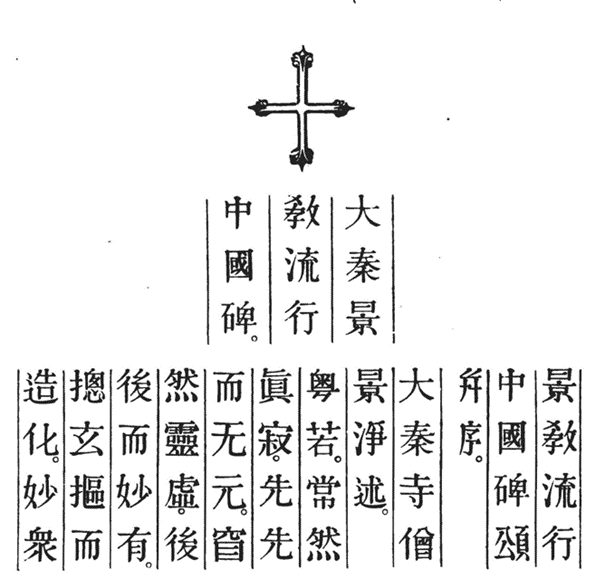
\includegraphics[width=\textwidth]{ChristologieCultureHistoire/Images/PremierParagrapheStele.png}
 
    \label{fig:my_label}
\end{figure}
 Si le livre d'Alopen 150 ans plutôt s'appelait simplement "Sûtra de Jésus-Messiah", le titre de la Stèle est le suivant :
\begin{quote}
    Monument rappelant la propagation à travers l'Empire du Milieu de l'Illustre Religion de Ta-ts'in. \cite{Havret:stelechretienne}
\end{quote}
Ta-ts'in (ou \emph{Da Qin}) indique l'Empire Gréco-Romain. Cette référence peut étonner quand on sait la répugnance des Eglises perses à être trop liées à Byzance. D'ailleurs, traditionnellement, le christianisme en Chine était appelé \textit{Bose Jiao}, l'\textit{enseignement Perse}.  En 745, il prend l'appellation officielle de religion de Da-Qin  possiblement par la chute de l'empire Sassanide perse un siècle plus tôt, qui rend caduque le terme de Perse, l'arrivée d'ambassades byzantines en Chine (attestée en 742) mais aussi par la référence à la philosophie grecque ainsi qu'à l'attribution de voyages en \textit{Da Qin} par le fondateur du Taoisme, Laozi :
\begin{quote}
    Calling Christianity the 'Religion of Da Qin' shows that the Nestorians of the Tang undeniably possessed a sensitive awareness of their political environment within China, and probably internationally as well, and moved with considerable acumen to secure the best possible position for themselves within it (\cite{Barrett:TaoismChristianity})
\end{quote}

\paragraph{Un découpage proposé en 25 sections} La stèle peut être découpée en 25 sections, la première sur les attributs de Dieu, puis les trois suivantes sur la Création et la Chute de l'homme (surtout pour développer l'idée d'un homme bon avant la chute par l'orgueil), puis les deux suivantes sur le Christ. A partir de la section 8, on trouve les caractéristiques de la religion, le baptême, les moines, l'éthique, puis plusieurs sections sur l'histoire des chrétiens en Chine, montrant une loyauté forte vis à vis des autorités politiques chinoises. Nous nous concentrerons sur les premières sections et en particulier les sections 6 et 7 proprement christologiques.  Il faut noter qu'une partie importante est liée à l'histoire du christianisme en Chine et la protection des empereurs. Cette attitude peut être mise en parallèle avec celle des premières communautés chrétiennes, avec Paul, montrant la compatibilité du christianisme avec l'Empire Romain (\cite{Baslez:MondeDevnuChretien}). 






\section{la partie proprement Christologique}

\subsection{Section 6 : l'incarnation} 

La première section qui nous intéresse parle de l'incarnation. Nous indiquerons à chaque fois les deux traductions en Français qui font foi (\cite{Havret:stelechretienne} et \cite{Pauthier:linscriptionSinganfou} \sn{la traduction de Havret est une traduction en latin et français mais la traduction française n'est pas complète - je l'ai complété à partir du texte latin}) :
 
\begin{tabular}{p{0.45\textwidth}p{0.45\textwidth}}
\\
Cependant, notre Trinité s'est comme multipliée, l'illustre et vénérable Messie, voilant et cachant son auguste majesté, se rendant tout semblable aux hommes, est venu en ce monde. les Puissances angéliques publièrent la bonne nouvelle; une femme vierge enfanta le Saint dans la grande Ts'in. Les esprits dans le Ciel annoncèrent la bonne nouvelle : "une Vierge a enfanté le Saint dans la grande Ts'in". Une étoile resplendissante a proclamé la faveur et la Perse, apercevant son éclat, vint lui faire hommage de ses présents. \cite[p. 35]{Havret:stelechretienne} & 

Ce faut alors que notre \textsc{Unité-trine} divisa sa personne dans le resplendissant et vénérable Messie, en voilant sa véritable majesté. il apparut dans le monde comme un simple mortel. Les Esprits dans le ciel annoncèrent la bonne nouvelle : "une Vierge a enfanté le Saint dans la Syrie !"  Une constellation resplendissante a proclamé l'heureux événement; les Perses ayant aperçu sa clarté, sont venus apporter leur tribut. \cite[p. 9]{Pauthier:linscriptionSinganfou} \\
                                                                                  
\end{tabular}
 
 \paragraph{Wo Sanyi, notre "trois-Un". } La pensée Taoiste utilisent le terme de Sanyi :  

\begin{quote} Le terme employé pour désigner la Trinité est un terme taoïste, \emph{sanyi} le "Trois-Un". mais pour signifier qu'il s'agissait de la Trinité Chrétienne, l'auteur de l'inscription a ajusté le caractère "\emph{Wo}" qui signifie "mon/notre". Ainsi le terme taoïste a pris un sens chrétien, "Notre Trois-Un".
    \cite[p.43]{Raguin:JesusMessieXian}
\end{quote}
Quelle est cette trinité taoïste ? Le Trois est pensé comme facteur d'harmonie entre l'Un et le Multiple permettant de «court-circuiter» la référence à Dieu ou à quelque instance supra-cosmique.\cite{Cheng:triadeChinoise}


Le terme utilisé pour le Christ est le terme syriaque de \textit{Messie}, translittéré et non traduit.

 "\textit{Voilant et cachant son auguste majesté, se rendant tout semblable aux hommes, est venu en ce monde}" est quasiment la traduction de Ph 2,6-7, soulignant l'abaissement du Christ.
 

\paragraph{Insistance sur le Ciel et l'environnement}  les cieux (\textit{constellation}) prennent une partie importante dans les deux sections sur le Christ, avec tout un passage sur l'Etoile des mages. On peut  déceler le souhait de l'auteur de montrer ce qu'est le Christ non pas en le décrivant directement comme \textit{forme},  causes ou \textit{logos} mais en insistant sur le \textit{fond},  \textit{le Ciel} qui \textit{ne s'exprime pas}. \cite[p. 109]{PolDroit:voyage} . 
\begin{quote}
    La philosophie gréco-européenne privilégie la « forme » – en grec ancien, \textit{eïdos}. Une « idée » est d’abord une « forme », qui se découpe sur un fond d’espace indifférencié. C’est ce fond d’espace qui retient l’attention chinoise, plutôt que la forme qui s’en détache. Scruter le fond plutôt que les formes, l’indifférencié plutôt que les différences, l’espace plutôt que les choses qui s’y trouvent et s’y découpent, telle pourrait être la première caractéristique de l’attitude chinoise.\cite[pp. 110-111]{PolDroit:voyage}  
\end{quote}
Dès lors, l'attitude des mages perses qui scrutent dans \textit{le Ciel} ce qui change, est finalement celle du sage Chinois. Pour le Taoisme, ce n'est pas par le discours, qui segmente et découpe mais par le biais d'histoires déroutantes, \textit{comme celle de l'étoile des mages}, que l'on peut transmettre la voie. \cite[p. 130-141]{PolDroit:voyage} 
 




\subsection{section 7 : la rédemption } 


Après l'incarnation, le texte développe en plusieurs paragraphes l'action de Jésus : 


\begin{tabular}{p{0.45\textwidth}p{0.45\textwidth}}
\\
Il accomplit les lois anciennes qu'avaient écrites les vingt-quatre Saints, direction des empires dans les conseils. Il fonda la nouvelle religion que la Trine unité, Esprit très pur, n'exprime pas au moyen de paroles, formant à la pratique des vertus par la vraie foi.  & Ainsi, s'est trouvé accompli ce que les vingt-quatre saints avaient annoncée dans l'ancienne loi : " le gouvernement des familles et des États par une grande et suprême doctrine. Il établit la doctrine pure de l'\textsc{unité-trine}, sans l'appeler une nouvelle religion. Il fortifia les bonnes habitudes par l'usage de la vraie foi. \\
\end{tabular}

\paragraph{Jésus est présenté comme un sage} Le texte insiste sur l'Esprit qui soutient la vertu sans passer par une loi (cf Jr 31,33 \sn{Jr 31,33 \textit{Je mettrai ma loi au dedans d'eux, Je l'écrirai dans leur coeur} \newline 2 Co 3,3\textit{Vous êtes manifestement une lettre de Christ, écrite, par notre ministère, non avec de l'encre, mais avec l'Esprit du Dieu vivant, non sur des tables de pierre, mais sur des tables de chair, sur les coeurs.}}  ou encore 2 Co 3,3).

Par cet  \textit{Esprit très pur, qui n'exprime pas au moyen de paroles formant à la pratique des vertus par la vraie foi}, l'auteur propose probablement une théologie accessible à la culture chinoise. pour les Chinois en effet,  ce n'est pas au moyen de raisonnements qu'on atteint le Ciel, qui s'éprouve directement
\cite[p. 117]{PolDroit:voyage} même si notre participation au Ciel en ce monde est parfois voilée.


Cependant, l'auteur ne s'arrête pas à une approche \textit{sans parole} puisqu'il mentionne les \textit{huit béatitudes} : 

\begin{tabular}{p{0.45\textwidth}p{0.45\textwidth}}
\\
Il institua les règles des huit fins, pour purifier les facultés et perfectionner les saints; il ouvrit la porte des trois principes,& Il posa les lois des huit limites morales que l'on ne doit point franchir. la poussière de la terre, purifiée comme le métal dans la fournaise, devint la vérité parfaite. Il enseigna au moindre les trois grandes vertus cardinales; 
\\ 
 en ouvrant les portes la vie et supprimant la mort. & il lui ouvrit les sources de la vie, et anéantit la mort.
\end{tabular}


 \paragraph{Référence à la Bible} Après avoir insisté sur l'éthique de Jésus, l'auteur met l'accent sur le corpus biblique, à la fois dans le registre de l'\textit{accomplissement} de l'Ancien Testament et ses 24 livres/ Saints mentionnés plus haut \sn{hors livres deutérocanoniques} que de l'annonce d'un nouveau Testament\sn{ l'auteur décompte 27 livres alors que le Corpus syriaque ne reconnaissait initialement que 22 livres (l'Apocalypse et les épîtres générales reconnus tardivement) }. 

 \paragraph{Sauver par le registre de la grâce} Face à poussière (Lieu-tch'en), expression bouddhique pour désigner les \textit{souillures de la pureté du coeur},  le texte mentionne les 8 lois morales (Pa-King, "8 circonstances"), comprises comme les Béatitudes (8 béatitudes chez Mt).  Sont aussi mentionnés la porte des trois vertus cardinales (Tch'ang), porte qui ouvre aussi à la vie et supprimant la mort (Mié-se) selon une expression chrétienne traditionnelle. 

Puis suit une expression typiquement bouddhique du soleil lumineux triomphant des porte des enfers (ti-yu) mot à mot \textit{prison de la terre} \cite[p. 49]{Havret:stelechretienne}.  Satan est ici appelé par le terme chinois \textit{Mo}, d'où la traduction de démon :

\begin{tabular}{p{0.45\textwidth}p{0.45\textwidth}}
\\
Il suspendit le soleil lumineux pour triompher de l'empire de ténèbres et {dès lors }les ruses du démons furent toutes pénétrées et déjouées
&  Il suspendit au ciel le brillant soleil de la vérité pour dissiper les habitations des ténèbres; les ruses mensongères du démon furent dès lors pénétrées et déjouées. \\
\end{tabular}



 
 
 

\begin{tabular}{p{0.45\textwidth}p{0.45\textwidth}}
\\
Conduisant à la rame la barque de la miséricorde, il s'éleva aux demeures lumineuses; dès lors quiconque possède une âme a trouvé son salut. L'oeuvre de la toute puissance étant ainsi consommée, il monta en plein midi, homme déifié.& Il mit en mouvement le navire de la miséricorde pour s'élever aux brillantes demeures; les âmes qu'il renfermait purent dès lors, en traversant le fleuve de la vie, obtenir cette fin glorieuse. A l'heure de midi, il s'éleva au séjour de la vérité. \\ Il laissait les vingt-sept livres de l'écriture, où est expliquée la grande réforme pour l'ouverture des \textit{ling-koan}
  \cite[p. 44]{Havret:stelechretienne} & 
Des saints livres ont été laissés au nombre de vingt-sept, qui ont étendu les conversions originelles en libérant les âmes.
  \cite[p. 10]{Pauthier:linscriptionSinganfou} \\
                                                                                  
\end{tabular}
 
  \paragraph{influence bouddhique du mouvement} Avec l'image de la barque de miséricorde (\emph{avalokites 'vara}), nous avons ici une belle image d'origine bouddhique, divinité plus connue en Chine sous le nom de \emph{Koan-yn} et surnommée \emph{Ta-t'se} la grande Miséricorde. D'après le bouddhisme, l'humanité tourne sans cesse comme sur une grande mer jusqu'à ce qu'elle arrive enfin au \textit{nirvana}. 
  
 % -----------------------------------------------
\section{Conséquences en terme de chemin de salut}

Quelles sont les conséquences sur le salut de cette étude rapide des deux paragraphes christologiques ?

\paragraph{Une dimension pratique du salut} Pour les chinois, la dimension pratique des débats est importante : 

\begin{quote}
    Entre ordre confucéen et contestation taoïste, il existe plus de complémentarité, malgré leurs désaccords, que d’opposition frontale. Ne perdant jamais de vue une dimension pratique, les débats chinois sont continûment traversés par des interrogations sur la bonté ou la méchanceté humaine, sur la bienveillance ou la cruauté nécessaire des souverains.

\cite[p. 147]{PolDroit:voyage}  
\end{quote}
 Regardons dans cet esprit le passage sur le mal qui précède les sections sur l'incarnation et la rédemption.
\begin{quote}
   Il arriva que Satan, disséminant ses fraudes, se para de l'ornement emprunté d'une pure essence, et qu'ouvrant une brèche dans cette grandeur morale, au milieu de cet heureux état, il y introduit la ressemblance de la confusion.
De là, des sectes aussi nombreuses que les jours de l'année, qui se suivirent pressées, et tracèrent à la suite leur sillon, tissant à l'envi les filets de leurs lois. les uns, désignant les créatures, s'appuyaient sur elles comme sur leur principe, les autres supprimant la réalité de l'Etre, se plongeaient dans la superstition, d'autres adressèrent des prières et des sacrifices pour attirer le bonheur, d'autres enfin firent parade de vertu pour en imposer aux hommes. 
\end{quote}
 
 
 Le péché introduit par Satan est décrit comme "ressemblance de la confusion". C'est un exemple de l'aspect concret du Chinois :\textit{ Tien-che }. \textit{Tien} signifie un ornement en métal; \textit{che}, chercher à paraître ce que l'on n'est pas ; se parer des dehors. La conséquence sont les \textit{sectes aussi nombreuses que les jours de l'année}; présentant les différentes voies de salut. On y a vu une critique du Taoisme (cette voie est accusé de diviniser les forces de la nature :  \textit{désignant les créatures, s'appuyaient sur elles comme leur principe}) et Bouddhisme aux tendances matérialistes et nihilistes (\textit{supprimant la réalité de l'Etre, se plongeaient dans la superstition}).  
 
 
 
 \paragraph{Par le Baptême, l'Esprit Saint nous éloigne des vaines gloires} Après la partie christologique, l'inscription développe les rites, d'abord le baptême, \textit{quittant les préoccupations vaines et mondaines pour obtenir la pureté}. Ce soucis d'humilité et de quitter le monde  rejoint la pensée du \textit{Chemin} ou \textit{Tao},  
 
 \begin{quote}
     à la fois faiblesse extrême (goutte d’eau) et puissance sans borne (océan). \ldots vent… C’est à force de faiblesse, si l’on ose dire, que le sage parvient à tant de puissance. 
\cite[p. 130 ]{PolDroit:voyage} 
 \end{quote}

Que ce soit dans la partie décrivant la chute ou au moment du baptême (et des vaines gloires), on trouve probablement une description adaptée aux oreilles chinoises, empreintes de la pensée Taoïste.

 Puis, l'auteur décrit la vie monastique : le rôle de la barbe et de la tonsure, images extérieures de la vie intérieure, l'absence d'esclave, l'égale considération de tout homme , le refus des richesses, la pratique de la générosité, le silence et la retenue. A ce titre, ils se présentent moins comme des moines bouddhiques que comme des sages pétris de sagesse confucéenne : 
 
 \begin{quote}
     Car le « mandat du Ciel », comme disent les confucéens, est présent avant tout dans le « sens de l’humanité » (ren) qui habite le cœur de chacun. Cette notion fondatrice, malaisée à définir, implique à fois, selon Confucius, d’être « juste dans le jugement », « conscient de la valeur de l’effort », « pacifique dans les conflits » et d’avoir de la « retenue ». Le \textit{ren} est ainsi l’instance de régulation des rapports entre les humains, agissant au cas par cas.

\cite[p. 122]{PolDroit:voyage}  
 \end{quote}
 Paul a préféré  l'aréopage au Temple, et les apologistes Chrétiens le terme néo-platonicien de  \textit{Logos} pour dire l'expérience du Christ et non les catégories des religions paiennes. De même, l'auteur de la \textit{Stèle} nous semble mettre en avant la sagesse confucéenne, plutôt que les moines Taoistes ou bouddhistes. Cette attention à la sagesse confucéenne explique peut être  la mention qui suit : les moines prient \textit{au secours des vivants et des défunts}, alors que la sagesse confucéenne accorde une importance forte au culte des ancêtres.
 
 

 
 
  
\paragraph{Ne pas penser séparément morale, rites privés et gestion des affaires communes} Une caractéristique importante de la civilisation chinoise est effet d’entrelacer doctrines morales, rites privés et gestion des affaires communes
\cite[p. 120]{PolDroit:voyage}. L'inscription développe non donc seulement le credo de la foi chrétienne (sections 7 et 8), mais aussi la morale et les rites (sections 9 et 10). A ces deux éléments s'ajoute la louange des empereurs chinois. Sur ce dernier point, les Chrétiens en Chine reprennent  la stratégie des chrétiens face à l'empire romain, qui s'inséraient dans le réseau de solidarité des villes par le rôle des évêques et des diacres (\cite{Baslez:MondeDevnuChretien}).


\section{Conclusion}

\paragraph{Une présentation du message Chrétien soulignant les aspects les plus accessibles à la pensée Chinoise} A travers l'étude de la Stèle, nous avons trouvé la présentation des principaux points de la Foi Chrétienne. Cependant, sans trahir le message chrétiens, l'auteur choisit une traduction qui résonne avec la culture chinoise. Au delà de la traduction, le choix des passages de la Bible comme \textit{l'Etoile dans le Ciel} ou l'accent sur certains points du rite comme la prière pour les défunts ou l'attention au \textit{Ren}, éclaire ce message chrétien de façon nouvelle. 
 
\paragraph{difficulté à penser l'acculturation religieuse} Dans nos recherches, nous avons rencontré des auteurs ne pouvant pas penser l'acculturation du message chrétien en dehors des catégories de l'hérésie. Ainsi, un article récent \cite{Gernet:Stele} s'oppose à l'interprétation d'une stèle de Xi'an acculturée à la culture chinoise et propose une clé de lecture basée sur un contexte de luttes théologiques internes au sein de l'Église nestorienne.

\begin{quote}
    rien ne prouve d'ailleurs clairement que les nestoriens aient songé à faire partager leurs croyances aux Chinois. [\ldots] Les circonstances et les mentalités étaient en effet tout à fait différentes de celle qui devait régner un millénaire plus tard, à l'époque de la contre-Réforme animée par une ambition de conquête universelle des esprits et des territoires (p. 245)
\end{quote}
Même si la communauté chrétienne qui a écrit la stèle était toujours fortement liée à l'Église perse - comme le montre les signatures de la stèle en araméen -, cette thèse nous parait difficilement acceptable à l'analyse. Les Eglises syriaques à cette époques nous sont certes assez mal connues; on peut noter l'importance du terreau judeo-chrétien à la création de ces Eglises, le milieu missionnaire parmi les marchands, la mixité culturelle, reflet des sociétés en monde iranien, la loyauté vis à vis des autorités politiques et le monachisme (\cite{Amir:CoranHistoriens}). Sans les relever tous, on retrouve de fait de nombreux éléments syriaque dans la Stèle (par exemple, influence des marchands et moines dans la création de l'Eglise de Chine), mais sans que cela ne remette en question le travail d'acculturation de la foi chrétienne en contexte chinois dont les marques sont soulignées par de nombreux sinologues. A tel point que c'est plutôt l'autre vision, celle d'une supposée trop grande acculturation qui est souvent soulignée (le P. Havret, sj note par exemple les 
\textit{    dangereux rapprochements} avec la culture Taoiste \cite[p.21]{Havret:stelechretienne}).   


Cette double polémique montre la difficulté à penser l'acculturation et sa conséquence en terme de christologie : notre vision du Christ est forcément transformée par l'acculturation, et elle peut être vécue sans être un dévoiement de la foi véritable, mais au contraire en développant des aspects du Christ qui sont restés comme en germe dans son incarnation en Judée "au temps d'Hérode" et qui peuvent se développer pleinement dans d'autres cultures et époques. 

%\chapter{Evolution de l'interdiction du \riba et Gharar}


a. Un dossier sur un thème lié au cours A partir de trois articles universitaires minimum. -  Introduction : intérêt du thème au regard de l’actualité et/ou de vos propres orientations personnelles ; présentation des articles et de leurs auteurs. Présentation du plan de votre travail. - Synthèse (ne pas présenter les articles séparément mais faire une synthèse à partir des différentes thématiques rencontrées) - Contextualisation de ce thème dans l’islam contemporain, éclairage par le contenu du cours (enjeux, dynamiques, etc). 

\section{Introduction}

En tant que membre du jury de l'Institut des Actuaires, j'ai eu à me prononcer sur certains mémoires présentés par des étudiants sur la \textit{finance Islamique} et \textit{l'assurance Takaful}. Ces mémoires ne couvrent pas les présupposés théologiques et commencent généralement par une présentation des interdits de la loi musulmane, comme par exemple ce \href{http://www.ressources-actuarielles.net/EXT/ISFA/1226-02.nsf/0/8c814ff5f2bae57ec1257e1a004407b6/\%24FILE/Memoire_ISFA_Tontines_et_Takaful_Bendimerad_Version_avec_Couverture.pdf}{mémoire d'actuariat} : 
\begin{quote}
     [pour faire face à ses  engagements, l'assureur],peut, par exemple, inclure des actifs obligataires dont les taux de rendement font apparaître des taux d'intérêt. [...] l'interdiction de l'usage du taux d'intérêt, appelé \textit{\riba} en arabe, est l'un des fondements du droit des affaires musulman.
\end{quote}
Dans la même veine, sont généralement définis les autres interdits, comme le \emph{Gharar}, défini dans le même mémoire comme : 
\begin{quote}
    Le contrat d'assurance peut constituer une perte disproportionnée en faveur de l'un des participants aux dépens de l'autre. Ce caractère d'incertitude, appelé \textit{Gharar} en arabe, est un caractère prohibé par l'Islam surtout lorsque le transfert du risque vers un tiers est total, ce qui est notamment le cas pour l'assureur qui porte entièrement la charge du risque cédé par l'assuré.
\end{quote}
Les mémoires d'actuariat consultés essayent de dépasser ces interdictions, qui soulignent une tension avec les \textit{Hadiths} : 

\begin{quote}
     
A l'issue de l'analyse précédente, l'idée même d'une assurance islamique semble être un contresens. Pourtant, la religion musulmane encourage l'individu à prendre des mesures pour réduire l'ampleur des désastres qui pourraient l'affecter. D'après un Hadith authentifié, le prophète conseille à un croyant de placer sa confiance en Dieu et d'attacher son chameau plutôt que de se limiter uniquement à placer sa confiance en Dieu en offrant la possibilité au chameau libre de s'échapper. L'Islam ne s'oppose donc pas à l'idée de vouloir minimiser les risques et par conséquent elle ne s'oppose pas à faire usage de la loi des grands nombres. Elle exclut certes la spéculation et l'incertitude ainsi que le taux d'intérêt. En revanche, elle compte parmi ses principes la coopération et l'entre-aide mutuelle ainsi que le partage équitable des risques et des bénéfices. Toutes ces bases ont permis de concevoir un modèle alternatif à celui de l'assurance conventionnelle.
\end{quote}
De cette tension naît des solutions techniquement assez complexes.


Intrigué par cette apparente clarté vis à vis de l'interdiction de l'\textit{intérêt} et de l'\textit{l'incertitude} à la base de l'économie moderne, je me propose d'étudier l'évolution de l'opposition de la \emph{\riba} et \emph{gharar} dans les différents courants de l'Islam contemporain, depuis la pensée d'Abduh jusqu'aux frères musulmans et le salafisme. 
L'interdiction des deux notions n'a pas la même importance économique et la \textit{\riba} a donné lieu à plus de développement. En partant de ces études, j'essayerais néanmoins de transposer ces travaux à l'assurance.
Après avoir regardé  à travers l'étude de ces deux notions comment l'économie moderne, pensée au XVIIIè et XIXè siècle questionne l'Islam, je poserai quelques pistes sur le propre questionnement du Christianisme. Après tout, le prêt à intérêt était aussi interdit au Moyen-äge en Europe (Concile de TOurs de 1163). Ces pistes seront en particulier nourries par l'étude de la pensée de Saint Thomas d'Aquin sur les taux d'intérêt et comment ces pistes peuvent nourrir la réflexion de la théologie musulmane (et chrétienne) contemporaine. 
 

%---------------------------------------------------------------------------------------------------------------
\section{Vision dans l'Islam Classique de l'interdiction de \riba}

\subsection{une interdiction de la \riba et Gharar}

Pour commencer, il est utile de se référer aux textes à l'origine de ces interdits.
\paragraph{Versets du Coran et Hadiths interdisant la \riba}
Le verset 130 de la Sourate 3, Al-Imran mentionne : 
\vocalize % switch diacritics for short vowels on
\transtrue % display the transliteration
\arabtrue % print arabic text (on by default)
\begin{quote}
 
\TArabe{
 يَا أَيُّهَا الَّذِينَ آمَنُوا لَا تَأْكُلُوا الرِّبَا أَضْعَافًا مُّضَاعَفَةً وَاتَّقُوا اللَّهَ لَعَلَّكُمْ تُفْلِحُونَ
  } 
   [3,125] O vous qui croyez !, ne vivez pas de la \textit{\riba} [produisant le] double deux fois ! Soyez pieux envers Allah ! Peut-être serez-vous bienheureux. 

\end{quote}
\begin{quote}
\TArabe{278
 يَا أَيُّهَا الَّذِينَ آمَنُوا اتَّقُوا اللَّهَ وَذَرُوا مَا بَقِيَ مِنَ الرِّبَا إِن كُنتُم مُّؤْمِنِينَ
279 فَإِن لَّمْ تَفْعَلُوا فَأْذَنُوا بِحَرْبٍ مِّنَ اللَّهِ وَرَسُولِهِ وَإِن تُبْتُمْ فَلَكُمْ رُءُوسُ أَمْوَالِكُمْ لَا تَظْلِمُونَ وَلَا تُظْلَمُونَ
} 
 [2, 278] O vous qui croyez !, soyez pieux envers Allah ! Faites abandon de ce qui [vous] reste [à toucher provenant] de la \textit{\riba}, si vous êtes croyants !
[2, 279] Si vous ne le faites point, attendez-vous à une guerre de la part d’Allah et de Son Apôtre ! si vous vous repentez, alors vous récolterez votre capital sans infliger ou être victime d’une injustice. \sn{Traduction de Blachière, sauf la dernière phrase \cite{ElGamal:BanqueFinanceIslamique}}

\end{quote}

De même, un hadith de Abu Hurayra met au même niveau la \textit{\riba} et le meurtre : 
\begin{quote}
    "Evitez les sept turpitudes !"

- "Quelles sont-elles, ô Envoyé d'Allah?", demandèrent les fidèles.


- "Ce sont, répondit-il :

 

-le polythéisme,

-la magie,

-le meurtre qu'Allah a interdit sauf à bon droit

-l'usurpation des biens de l'orphelin,

-la \textit{\riba},

-la fuite du front au jour du djihad et

-la fausse accusation (de fornication) des femmes vertueuses, chastes et croyantes".
\end{quote}
 
  Nous avons évité à ce stade de traduire le terme de \textit{\riba}, par \textit{usure} ou \textit{intérêt}. Le Hadith rapport par at-Tirmidhî a été utilisé pour appliquer le sens d'intérêt à la \textit{\riba}  : 
 \begin{quote}
     Vendez de l'or contre de l'argent (les quantités échangées étant) comme vous voulez, à condition que ce soit main à main. Vendez du blé contre des dattes sèches (les quantités échangées étant) comme vous voulez, à condition que ce soit main à main. Vendez de l'orge contre des dattes sèches (les quantités échangées étant) comme vous voulez, à condition que ce soit main à main (n° 1240)
 \end{quote}  
 On peut effectivement y lire le refus de l'intérêt mais d'autres lectures sont possibles, en particulier en relevant l'insistance du hadith à une transaction \textit{main à main}, qui permet une transaction claire. Par ailleurs, la valeur du temps n'est pas explicitement mentionnée.
 

 
\subsection{un nouveau contexte avec la naissance du Capitalisme}
Du point de vue du prêteur, le prêt à un prix du fait du risque  que l'emprunteur repaye le prêt, la valeur temps (qui correspond à l'inflation et à la perte d'opportunité d'un investissement aujourd'hui qui rapporte plus plus tard). La pertinence économique de l'intérêt et de la prise de risque est donc justifiée même si cela ne veut pas dire qu'elle l'est d'un point de vue religieux.
Avec l'accumulation des richesses dans les villes italiennes au moyen-âge naît le capitalisme et la finance : comment financer et assurer les bateaux partant de Gênes et remplis de richesse ? Cette irruption de la finance pose de nouvelles questions.  Face à cette accumulation, une réponse théologique chrétienne sera la création de l'ordre mineur par Saint François d'Assise. Et, nous reviendrons sur ses développements, la réflexion de l'université de Paris et de Saint Thomas d'Aquin sur la notion d'usure et de juste prix.  
Ces innovations touchèrent tardivement le monde musulman, au XIXème, avec l'arrivée simultanée de l'industrialisation, qui nécessite des capitaux importants et les débuts de la colonisation. Par l'industrialisation, la capacité productive est fortement augmentée par l'investissement, mais aussi la concentration des risques qui ne peuvent être portée par la solidarité traditionnelle.
Face à cette nouvelle question, quelles sont les réponses proposées par les théologiens musulmans depuis l'arrivée de cette question ?


%---------------------------------------------------------------------------------------------------------------
\section{Elements théologiques apportés}

\subsection{Premières réponses face à la nécessité du prêt}
\paragraph{Le développement du \riba et de l'assurance par les Occidentaux} Les prêts à intérêt ont toujours existé au sein de l'Empire Ottoman\cite{Gilbar:Qadi}, et proposés par des familles grecques, arméniennes ou Juives (et en Iran par les arméniens et zoroastriens). A ce premier Groupe, s'ajouta les banques commerciales européennes ou les banques "étrangères-locales" comme la banque impériale ottomane au XIX.
De la même façon pour les assurances, Ibn Abidin, représentant de l'école officielle de droit Hanadi dans l'empire ottoman, suggère le compromis suivant : il est licite d'établir ds contrats d'assurance portant sur les risques encourus à l'intérieur du royaume islamique - le Dar al Islam -à condition que ces contrats soient conclus avec une compagnie d'assurance ayant son siège hors de pays de l'Islam. 

\paragraph{Utilisation de prêt à intérêt par les musulmans malgré l'interdiction du \textit{\riba}.} La \textit{\riba} a pu poser des problèmes dans son implémentation, en particulier pour les grands marchands (tujjār).  
Pour l'école Hanafite, le terme de \riba peut être traduit par usure, dans le sens d'un taux d'intérêt exhorbitant, à l'opposé de l'intérêt raisonnable, le \emph{ribh}. L'autre interprétation dominante, attribuée à 'Abdahallah Ibn 'Abbas, permet d'expliquer la notion du Coran de double capital par la pratique du \textit{\riba al jâhiliyya} (préislamique), avec des taux d'intérêt très élevés avec des intérêts pouvant dépasser le capital en cas de non-paiement. A l'opposé de ces analyses plus ouvertes, la position de l'école Hanbalite fut l'interdiction pure de l'intérêt. Pour contourner l'interdit du \riba face à la nécessité, les marchands musulmans mirent en place des montages complexes où l'intérêt était déguisé en une \textit{double vente} (\emph{mukhâtra}) avec deux ventes fictives successives permises par la \textit{sha'ia}: 
\begin{itemize}
    \item la première, le préteur vent un objet à l'emprunteur pour une somme équivalente au capital et à l'intérêt. l'emprunteur s'engage à payer la valeur de l'objet à la fin de la période (techniquement, une vente avec paiement différé). 
    \item A la fin de cette première transaction, l'emprunteur revend le même objet pour la valeur du principal (techniquement, une vente à terme).
\end{itemize}
 Cependant, l'étude des jugements des cours religieuses au moyen-orient entre le XVI et le XVIII montre que malgré ces montages, des exemptions partielles ou totales de paiement de l'intérêt du fait de son incompatibilité avec l'Islam \sn{GILBAR, GAD G. “The Qadi, the Big Merchant and Forbidden Interst (Ribā).” British Journal of Middle Eastern Studies, vol. 39, no. 1, 2012, pp. 115–36, http://www.jstor.org/stable/23264404. Accessed 3 May 2022.}
 

\section{la pensée d'Abduh et Rida}
\subsection{position d'Abduh} Le Cheikh {Muhammad Abduh} (1849 - 1905) Egyptien, successeur d'Al Afghani, est la figure marquante du réformisme islamique. Il s'oppose au colonialisme atteignant alors l'Egypte. Son séjour  parisien le convainc de la nécessité de réforme de l'Islam et l'initie aux réflexions intellectuelles occidentales et en particulier François Guizot. A sa suite, il il pense l'Islam comme civilisation et pas uniquement comme Religion, avec la notion de progrès lié à la civilisation. Il n'y a pas d'opposition pour lui entre Foi et Raison, la religion musulmane étant \textit{raisonnable}.    Dans son livre \citet{Abdou:Rissalat}, il part de la Raison pour montrer le besoin que l'homme ne se fixe pas sa propre loi.

Il montre tout d'abord la naissance des besoins et des liens entre les hommes. Idéalement ces liens seraient ceux de l'amour : 
\begin{quote}
    Nul ne met en doute que chaque membre d'une société a besoin
des autres membres; et chaque fois que l'individu accroître ses exigences
dans la vie il ressent plus fortement le besoin de recourir au concours
de ses semblables. Ainsi se développent les besoins et à leur suite s'étendent
les relations de la famille à la tribu, de celle-ci à la nation, et finalement
au genre humain tout entier, comme le montre notre époque . Ces
besoins qui créent dans le sein de chaque nation (surtout dans le sein de
celles qui méritent vraiment ce nom) des relations et des rapports
spéciaux la distinguant des autres nations, sont le besoin de se procurer
sa subsistance, celui de profiter des biens de la vie, celui d' acquérir
les choses désirables et d'éloigner de soi celles qui déplaisent. 
Si la vie de l'homme se déroulait selon les lois de la nature, telles
que nous les voyons appliquées aux autres êtres vivants, les besoins
que nous venons de citer auraient été parmi les facteurs les plus puissants
de l'amour entre les individus[...].  

[\ldots]
Si par contre, l'intérêt se mêle aux relations amicales, et si chacun des amis exige un prix pour son amour, celui-ce se change en esprit d'exploitation, il se reporte sur l'effet utilitaire et se transforme chez l'un des amis en un abus de la force, et chez l'autre, en peur avilissante, en dissimulation et en hypocrisie.
\cite[p.66]{Abdou:Rissalat}
\end{quote}
Mais l'homme ne vient pas selon les lois de la nature car il est inconstant : 
\begin{quote}
 l 'homme
a été créé avec un caractère inconstant; quand le malheur l'atteint
il est abattu, et quand il acquiert quelque bien il devient insolent.
(C. ch. 70, v. 19 à 21). [...]
Chaque fois que la mémoire et l'imagination les poussent à
éviter quelque chose qui leur inspire de la crainte ou à atteindre un
objet qui leur fait envie, leur intelligence leur ouvre une porte de la
ruse ou leur découvre une voie de la violence ; alors le rapt remplace
l'échange pacifique, la dispute prend la place de l'union et la conduite
de l'homme riche s 'appuie plus que sur l'astuce et la violence.
\cite[p 68]{Abdou:Rissalat}
\end{quote}
il montre qu'on peut accéder à l'équité par des voies naturelles mais qu'à la foi pour les masses et pour éviter la corruption des élites, il est nécessaire de s'appuyer sur loi externe.
\begin{quote}
[...] ] le genre humain
a surtout besoin, pour conserver son existence, de l'amour ou d'un
sentiment qui le remplace.
A différentes époques il y a eu des penseurs qui ont fait appel à
l'équité ; ils ont pensé, et même quelques mystiques ont exprimé cette
pensée par de nobles paroles, que l'équité remplace l'amour. Cette
assertion ne manque pas de sagesse, mais qui est-ce qui peut établir les
règles de l'équité et amener la totalité des hommes à se soumettre ?
\cite[p 69]{Abdou:Rissalat}
\end{quote}

Suivre la Loi de Dieu, ordonner le bien est alors supérieur à la foi : 

\begin{quote}
  le Coran indique
qu'il n'y a pas de condition meilleure que celle des hommes qui ordonnent
le bien et défendent le mal: \begin{quote}
    Vous êtes les meilleurs parmi les hommes,
vous ordonnez le bien, vous défendez le mal et vous croyez en Dieu. (Cor. ch. 3, v. 106.) 
\end{quote} 
 
Dans ce verset le fait d'ordonner le bien et de
défendre le mal est mentionné avant la foi en Dieu, bien que la foi soit la base même sur laquelle s'appuient les bonnes oeuvres. 
\cite[p 121]{Abdou:Rissalat}
\end{quote}

\paragraph{Conséquence pratique pour la \riba}
'Abduh liste alors une liste de maux que l'Islam permet d'éviter : 
\begin{quote}

[l'Islam] nous invite par dessus tout à dépenser notre bien pour les oeuvres
charitables et souvent il en fait l'expression de la foi et la manifestation
d'une bonne conduite; il déracina par là, du coeur des pauvres, la rancune
et la haine contre ceux que Dieu a favorisé des biens terrestres ; il leur
inspira l'amour pour les riches, tout comme il fît naître dans le coeur de
ceux-ci la pitié pour les malheureux ; ainsi il développa la confiance dans
le coeur de tous les hommes. Quel remède plus efficace contre les maux
dont souffre la société: « C'est une faveur que Dieu accorde à qui il veut,
car Dieu est d'une bienfaisance sans bornes. » (Cor. ch. 57, v. 21.)
\textbf{L' Islam a fermé les deux portes du mal, il a bouché les deux sources
qui minent l'intelligence et détruisent la richesse, en frappant les boissons
enivrantes, les Jeux de hasard et l'usure, d'une interdiction absolue qui
n'admet pas d'infraction.}
\cite[p 122]{Abdou:Rissalat}
\end{quote}
Ainsi, parmi ces maux figure la \riba traduit ici par \textit{usure}.

\paragraph{Pratiquement : l'avis d'Abduh sur l'ouverture de la Caisse d'Epargne en Egypte}
L'ouverture de la Caisse d'Epargne et la répugnance d'un certain nombre de musulmans à toucher les intérêts poussèrent la caisse d'épargne à demander à 1903 une Fatwa à Abduh \cite{Jomier:AdbouCaisseEpargne}. Cette fatwa semble n'avoir jamais existé. En revanche, Ce fut à la requête d'un particulier mais en fait pour la
Compagnie d'Assurances sur la vie Gresham. La Compagnie d'Assurances al-Chark,
au Caire,  conservait une copie d'une fatwa d'Abduh \textit{écrite initialement pour un particulier} afin de la montrer à ses clients, le cas échéant. Le
client effectue des versements réguliers et périodiques par tranches successives
prévues d'avance ; la compagnie les encaisse et se charge de faire fructifier cet
argent. Finalement, à l'échéance, la société remboursera le total des versements
effectués augmenté des bénéfices résultant de la fructification. La fatwa admet
la licéité d'une telle opération en des termes qui, au fond, s'appliqueraient à toute
société en commandite. Il faut noter que la revue Al-Manâr de \textit{Rashid Rida} ne nia pas l'authenticité de cette fatwa après la mort d'Abduh mais protesta contre l'extension faite à toute assurance vie.

\paragraph{la note de la revue Al-Manâr de 1903}


Face aux scrupules de 3000 musulmans à toucher les intérêts (fa'ida), un échange eu lieu entre le directeur de la Caise d'Epargne et Abduh, échange repris par la revue \textit{Al-Manâr}. Abduh y maintenait fermement le principe de
l'interdiction absolue de l'usure (al-ribâ) ; mais il ne classait pas le cas de la Caisse
d'Epargne avec ceux de l'usure. Il l'assimilait à celui d'une société en commandite
(chirkat al-mod'âraba). A la suite de cette discussion, la loi fut modifiée en 1904 : 
 

\begin{quote}
 Il est prévu dans l'article premier que le client devra signer un
formulaire imprimé dans lequel il déclarera donner au Directeur Général de la
Poste tout pouvoir pour faire fructifier les sommes déposées, d'une façon licite et
en excluant toute opération usuraire. Il déclare permettre au Directeur de la Poste
de joindre ses dépôts à ceux des autres clients pour les faire fructifier en commun
à condition de recevoir une part de bénéfices (al-ribh') proportionnelle à ses
versements. On notera que dans cet article comme dans tout le reste de la loi le
mot de \textit{fâ'ida}, intérêt, est totalement absent. \cite{Jomier:AdbouCaisseEpargne}
\end{quote}

\begin{quote}
    L'article deux stipule entre autres ce qui suit. Il évite de parler de tant pour
cent, formule qui rappelle trop les intérêts. Il note que la part des bénéfices ne
dépassera pas un pour quarante du capital et le surplus, s'il y en a, reviendra à
l'administration postale à titre de compensation pour les services rendus et les
frais que ceux-ci comportent. L'assimilation à la société en commandite est ainsi
mise en accord avec le fait que la proportion des bénéfices touchés est fixe. On
notera que la proportion de un pour quarante est familière aux oreilles des
musulmans pieux puisque dans un certain nombre de cas le montant de la Zakat
atteint ce chiffre.
\end{quote}

On voit donc la position d'Abduh comme ferme dans les principes et ouvert dans l'application, même si cela se traduit par une subtilité juridique.


% - ----------------------------------------
\subsection{L'approche de Rashid Rida sur la \riba} 

Rida est l'un des successeurs spirituels de Abduh. Il fonda avec Abduh la revue néo-réformiste al-Manâr en   1898. Elle définit sa politique éditoriale à l’égard « de la civilisation occidentale » sous forme de deux impératifs : 
\begin{quote}
    \item  1/ Il faut que la terre musulmane puisse rattraper l’Europe sur le plan des sciences modernes, de l’industrie et de l’innovation technique. 
    \textbf{ }2/ En contrepartie, il faut déclarer une guerre sans merci à tout ce qui a accompagné l’entrée des Européens en terre musulmane comme décadence morale et mauvaises mœurs
\end{quote}

\paragraph{Une lecture de la \riba originale à la base de l'économie Islamique } face au développement des banques avec intérêt dans tous les pays colonisés et particulièrement en Egypte, il est important pour Rida de refonder les principes sous-jacents à l'intérêt et à l'économie financière \cite{Siddique:DemystifyingRiba}. Face à des lectures libérales (\riba comme usure) et à l'opposé, les musulmans socialistes (\riba comme profit), il existe une position médiane mais qui mérite d'être précisé : 


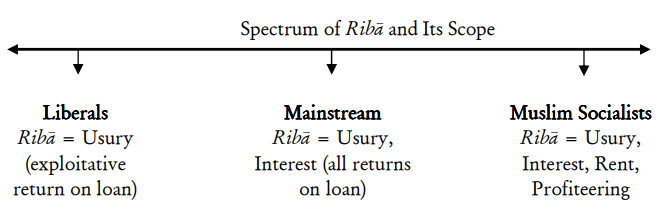
\includegraphics[width=0.9\textwidth]{CourantsIslamContemporain/ImagesCourantsIslamContemporain/Riba.png}

Rida part de l'analyse du mot \riba comme \textit{excès}, et en particulier reprend l'analyse de Co 3,125 présentée au début d'un excès lié à la renégociation de la dette. De là, il conclut que ce qui est interdit par le Coran sont les intérêts ajoutés à la fin de la période de prêt (\riba ’l-jahiliyyah). D'une certaine façon, ce sont les intérêts composés qui sont interdits, le fait que les intérêts augmentent en cas de non paiement. Cela lui permet d'autoriser les intérêts bancaires :
\begin{itemize}
    \item ils ne doublent pas les taux
    \item l'ajout d'un intérêt fait partie du principal de la même façon que le prix d'une vente à crédit (\emph{\riba al-buyu}) qui ne sépare pas principal et intérêt et qui est autorisé par le Coran.
\end{itemize}
 Il fait une distinction entre la \riba interdite dans le Coran et celle des Hadiths (voir graphique \ref{fig:MinorityRiba}) :

 \begin{figure}[h!]
     \centering
     \sidecaption{\cite{Siddique:DemystifyingRiba}, une séparation entre Coran et Hadith}
      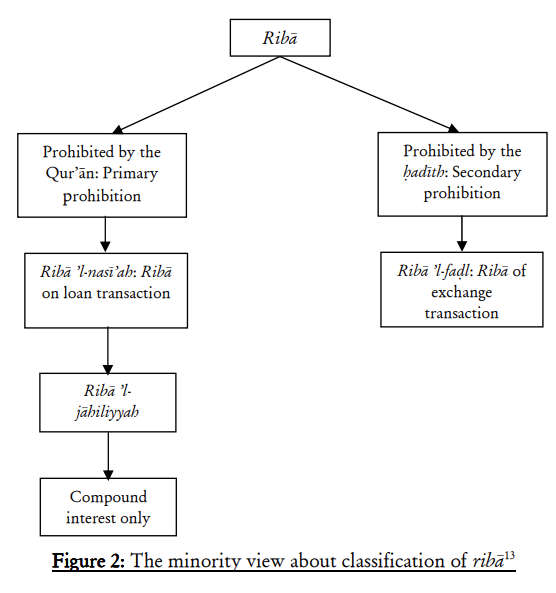
\includegraphics[width=0.5\textwidth]{CourantsIslamContemporain/ImagesCourantsIslamContemporain/RibaRida.png}
      \caption{La présentation du Riba selon Rida, dite minoritaire}
     \label{fig:MinorityRiba}
 \end{figure}
 
 Rida ne sera pas suivi par une majorités de jurisconsultes sur la légitimité des taux d'intérêt. En revanche, ils adopterons sa distinction entre less différents \riba, en étendant l'interdiction de la \riba du Coran à tout intérêt et pas seulement intérêt d'intérêt. Mais du coup, se pose la question du Hadith : pourquoi interdit-il  la \rib \emph{Al-Fadl}, c'est à dire la di
 
 

 
\paragraph{Les frères musulmans}
Dans les perspectives du réformisme musulman,
cette question d'ailleurs est loin d'être insoluble car une société qui émet des
actions peut être assimilée à une société en commandite. Les dividendes
représentent alors la part des bénéfices proportionnelle au capital engagé... 
al-Banna, fondateur des Frères Musulmans en Egypte, avait admis la licéité de ce
genre d'opérations et des Frères avaient, peu avant 1 948, fondé quelques ateliers
ou sociétés financées par ce procédé (2). La difficulté principale vient de ce que la
langue arabe n'a pas de mot spécial pour désigner les dividendes et que le terme
fâ'ida a des relents de ribâ.
\begin{quote}
    III. 2 interdiction de pratiquer l'usure, orienter les banques vers cette interdiction, le gouvernement doit donner l'exemple en abandonnant l'\textit{intérêt} fixé par les banque du prêt et du prêt industriel, etc. \textit{programme des frères Musulmans, 1936}
\end{quote}
%---------------------------------------------------------------------------------------------------------------
\section{Naissance de la finance et de l'assurance Islamique}

\subsection{Ce que l'on voit : Malaisie,...} 

\paragraph{une pratique supposant une \textit{shari'ah} qu'on ne peut interroger}

\subsection{Quelle est la théologie sous-jacente}

\paragraph{Une évolution de la shari'a par les principes} Mohammed Talbi 
\begin{quote}
    Il existe
trois principes en islam permettant de faire évoluer le droit et de
l'adapter
à la réalité, 

la \emph{maslaha} c'est-à-dire l'utilité publique, un
concept qui date du II\textsuperscript{e} siècle de l'hégire, 

la
\emph{zharoura}, la nécessité, c'est un principe fort puisqu'il est dit
que "la nécessité rend permis l'interdit" ; 

et les \emph{maqassid}, les
finalités de la loi. 

\begin{Synthesis}
On part des principes contre les principes. 
\end{Synthesis}
\sn{voir p. \pageref{TroisPrincipesEvolutionsShari}}
\end{quote}


\section{Conclusion}

\paragraph{une variété importante de vision mais toujours basée sur la sharia}

\paragraph{une réflexion sur la base de la Sharia'}
voir ce que Candiard dit de ce théologien qui dit de ne pas faire de Kalam mais du droit.

\paragraph{quel pourrait être les pistes de Kalam, quelques pistes de l'expérience occidentale ?}

\paragraph{St Thomas et l'usure : une réflexion autonome de la théologie}

\paragraph{extension du juste prix dans les risques : la dimension actuarielle}
\paragraph{Au XIXème, réflexion neo-thomiste et patristique pour sortir du carcan}
Après avoir regardé comment l'économie moderne, pensée au XVIIIème et XIXème questionne l'Islam à travers l'étude des différents courants de l'Islam contemporain, je poserai quelques pistes sur le propre questionnement du Christianisme. Après tout, le prêt à intérêt était aussi interdit au Moyen-äge en Europe. Ces pistes seront en particulier nourrie par l'étude de la pensée de Saint Thomas d'Aquin sur les taux d'intérêt et comment ces pistes peuvent nourrir la réflexion de la théologie musulmane. 

Nous catholiques au XIX par rapport à la modernité: renouveau thomiste et patristique. Liberté de pensée par rapport aux questions de l’époque
« A quoi on tient en vrai »
Le raccourci de certains théologiens musulmans : faire le court circuit pour repenser les choses : obsession juridique. Comment on sort du droit ? En faisant de la théologie. Et pour cela retour à la tradition
Voile
Le coran la dit donc il faut se voiler. Voile : hijab n’est pas dans le coran. Rideau
Zina : qu’il faut cacher
Jilbab pour les filles et femmes du prophète 
Ibn el jahouzi : voile non mentionné. Dimension non religieuse

Des écrits au XX. Deux raisons : les femmes vont occuper plus de rôle dans l’espace publique.
Et renouveau de l’anti théologie. Le voile est une question de théologie. Question de la foi
	⁃	Saint Paul : la foi et les œuvres
	⁃	On comprend croyant non pratiquant
	
%\chapter{Matériaux bruts pour validation}

\section{A lire}
\href{https://www.persee.fr/doc/ridc_0035-3337\_1955\_num\_7\_3\_9521}{Le prêt à intérêt et l'usure au regard des législations antiques, de la morale catholique, du droit moderne et de la loi islamique }

\section{Refus de l'intérêt en milieu chrétien}

\subsection{1163 : le concile de Tours condamne le prêt à intérêt}


Le 01 septembre 2014

La condamnation du prêt à intérêt par l'Eglise n'a pas empêché, au travers de divers subterfuges, le développement du crédit, moteur de l'activité économique.

Dans l’Occident chrétien médiéval, le rôle de prêteur sur gages, souvent pour de faibles montants, sera longtemps assuré par des juifs, que leur religion autorise à prêter avec intérêt à des non-juifs. Mais dès le XIe siècle, de nombreux bourgeois chrétiens enrichis se livrent au prêt à une autre échelle. Déjà au XIIe siècle, des bourgeois d’Arras, de Cahors, des Lombards d’Asti, des Génois prospèrent par ces opérations.

Certes, l’Eglise et les princes qui se conforment à sa loi bannissent le prêt à intérêt en s’appuyant - entre autres - sur l’Evangile de Luc : "Prêtez-vous l’un à l’autre sans rien en attendre." En France, le concile de Tours de 1163 condamne une des formes du prêt à intérêt dans le cadre de la moralisation de l’Eglise : nul clerc (évêque, abbé) ne peut désormais prêter de l’argent et recevoir en gage un

\section{Extrait site internet}
\begin{quote}
En Islam, le Riba est interdit : il s’agit de l’un des plus grands péchés, qui tire son origine du Coran. Mais il est également l’un des plus banalisés. Le Riba, appelé « usure », désigne l’intérêt perçu sur de l’argent prêté. De nos jours, le Riba est partout présent dans le domaine financier, à savoir, dans les comptes d’épargne, dans les prêts à intérêts, dans les agios… Alors, qu’est-ce que le Riba exactement ? Pourquoi est-il interdit ? Comment financer vos projets sans Riba 
\paragraph{Définition du Riba}

Le Riba peut être défini par intérêt - usure. Si le terme « usure » est la traduction la plus fréquemment donnée à cette interdiction de l’intérêt usuraire, il est important de préciser que le mot Ribâ vient cependant du verbe rabâ \& arbâ qui signifie augmenter et faire accroître une chose à partir d’elle-même. 

Dans le contexte financier, il est donc interdit de réaliser des transactions financières basées sur du Riba. Or, lorsque vous possédez un compte courant conventionnel, l’argent qui y transite alimente un circuit basé essentiellement sur l’usure. En effet, dans ce contexte, la banque dispose de vos fonds afin de spéculer. Même principe lorsque vous êtes à découvert : les agios que vous devez payer vous impliquent dans la pratique de l’usure.

Mais ce n’est pas tout : lorsque vous épargnez votre argent sur des comptes de type livret Jeune, Livret A, ou PEL, les intérêts que vous touchez sont également basés sur la pratique du Riba, et cela que vous fassiez don ou non des intérêts.

Enfin, lorsque vous réalisez un prêt bancaire, vous participez au développement de l’usure en payant des intérêts. 

\paragraph{De nombreux versets du Coran interdisent la pratique de l’usure.}     En voici quelques-uns, qui sont particulièrement explicites :

Verset 130 de la Sourate 3, Al-Imran : « Ô les croyants ! Ne pratiquez pas l’usure en multipliant démesurément votre capital. »
Les versets 278 et 279 de la Sourate 2, Al-Baqarah : (V-278) « Ô les croyants, craignez Allah ; et renoncez au reliquat de l’intérêt usuraire, si vous êtes croyants. (V-279) Et si vous ne le faites pas, alors vous recevrez l’annonce d’une guerre de la part d’Allah et de son prophète. Et si vous vous repentez, vous aurez vos capitaux. Vous ne lèserez personne, et vous ne serez point lésés. »
D’après Abu Hurayra, le Prophète (SAWS) a dit : « Evitez les 7 turpitudes ». Lorsque les compagnons demandèrent : « Quelles sont-elles, Ô envoyé d’Allah ? », il mentionna l’usure aux côtés notamment du polythéisme, du meurtre…
D’après Sahih Muslim : Ubâdah Ibn As-Sâmit rapporte que le Messager d’Allah (SAWS) a dit : « Or pour Or, argent pour argent, blé pour blé, orge pour orge, datte pour datte, sel pour sel, de manière égale, de main en main. Si la nature des produits diffère, vendez comme vous le voulez, si c’est de main en main ». \sn{\href{https://firstunion.fr/quest-ce-que-le-riba/}{First Union} ? }
\end{quote}

 
 \paragraph{Abd ar-Rahman ibn Nasir as-Sadi}\href{https://fr.wikipedia.org/wiki/Abd_ar-Rahman_ibn_Nasir_as-Sadi}{Abd ar-Rahman ibn Nasir as-Sadi} Oulema Hanbalite saoudien 1889. influencé par 	
Ibn Taymiyya
Mohammed ibn Abdel Wahhab
 
 \paragraph{ Le ribâ (l’usure) dans l’Islam}
 
 \href{https://www.ajib.fr/le-riba-lusure-dans-lislam/}{Le riba est l'usure dans l'Islam}
 
 \begin{quote}
    


Pour comprendre le sens réel du ribâ, pour connaître son statut légal dans l’islâm, houkm, qui est bien sûr, l’interdiction, ainsi que les méfaits individuels et collectifs qu’il engendre, il faut comprendre quelques points importants.

Parcourons ensemble ces extraite du livre « Le résumé des vertus de la religion musulmane » du grand savant \textit{Abdarrahman As-Sacdî} qui nous éclaireront sur la vue de la législation islamique, \emph{shariah}, sur les transactions, licites et illicites, ainsi que la sagesse du Législateur, Allah, soubhânah, en établissant cette auguste législation.

Nous verrons en particulier, les problèmes qui concernent le ribâ.

\begin{quote}
    
Que signifie le ribâ ?

Le ribâ signifie l’usure. Si l’on entend par « usure » le prêt à taux supérieur à zéro.

Car la définition contemporaine de « l’usure » est « l’intérêt excessif » ou « l’intérêt supérieur au taux légal », tandis que le ribâ est le prêt à intérêt, aussi minime soit-il.

Le prêt islamique légal est donc le prêt à zéro intérêt. Et le ribâ est l’usure dont l’intérêt est supérieur à zéro.

Il y a plusieurs types de Ribâ :
\begin{itemize}
    \item 1/Le prêt à intérêt : le surplus, aussi minime soit-il, perçu, pour le prêt, par le créancier en échange du délai accordé.

 \item 2/Ribâ al-fadhl : le surplus perçu lors de l’échange d’un bien ribawî (relatif au ribâ) tel que l’échange de l’or avec l’or, de l’argent avec l’argent, du blé avec le blé… etc.

 \item 3/Ribâ an-nasî’ah : différer l’encaissement lors d’un échange d’un bien ribawî de même nature, tel que l’or avec l’or, ou de nature différente, mais dont la cause ribawique est commune, tel que l’or avec l’argent.
\end{itemize}


\paragraph{Quelles sont les transactions dites légales dans le \emph{shariah}, halal ?}

La vente rendue licite par la législation islamique ainsi que le louage[1], les sociétés et les différentes transactions ; celles où s’échangent les marchandises entre les gens, les dettes, les utilités… etc.

\paragraph{Pourquoi une transaction est légale dans le \emph{shariah}, dite : halal ?}

La législation parfaite a permis ce type de transaction et l’a autorisé aux hommes, car cela assure leurs intérêts – nécessaires, indispensables ou complémentaires -.

Elle a élargi ainsi considérablement la liberté des hommes afin que leurs affaires et leurs conditions se réforment et que leurs vies s’ordonnent.

Quelles sont les conditions de la légalité d’une transaction ?

\textbf{La législation, \emph{shariah}, posa comme conditions pour que les transactions soient licites :}

1-La satisfaction des deux parties ;

2-la clarté du contrat ;

3-la connaissance de l’objet du contrat, de la durée du contrat et des conditions qui en résultent.



Quelles sont les transactions interdites dans la \emph{shariah}, dites : haram ?

La législation, \emph{shariah}, a interdit tout ce qui comporte un préjudice ou une injustice tel que :

1-Les différents types de jeu de hasard,

2-le Ribâ ;

3- l’ignorance[2], la jahâlah.
\end{quote}
 

Cette division, licite et illicite, halal et haram, prescrite par Allah et révélée à Son Prophète Mouhammed, ainsi qu’à tous les Prophètes avant lui, a pour objectif essentiel de préserver le but premier escompté par ces opérations d’échange entre les humains : l’intérêt mutuel, l’avantage commun à toutes les parties de l’échange et le bénéfice pour tous.

Inversement, tout ce qui n’apporte pas d’intérêt commun et ne fait pas bénéficier toutes les parties qui opèrent la transaction est illicite, haram et interdit.

Car cela va à l’encontre de la raison de cette opération d’échange, la transaction, qui est l’intérêt commun et l’absence de préjudice.

\textbf{Le ribâ fait partie de cette catégorie car son intérêt va dans un sens unique, qui est celui de l’enrichissement du créancier, et il porte un préjudice considérable au débiteur.}

Ceci s’appelle : injustice, iniquité et celui qui en profite ne fait que manger l’argent et les biens des autres injustement.
 \end{quote}
 
 
 \paragraph{Dictionnaire du Qoran}
 

 \section{Demystifying Riba through the Methodology of Muslim Jurists}
 \href{https://www.proquest.com/docview/2352353188?accountid=143046&parentSessionId=Sg7rHgjzHS0M9aF4pv1Nx2pxOOyR5LkKvILKrOVqG1o\%3D&pq-origsite=summon}{Demystifying Riba through the Methodology of Muslim Jurists}\sn{MUHAMMAD ZAHID SIDDIQUE; MUHAMMAD MUSHTAQ AHMAD.
Islamic Studies; Islamabad Vol. 58, N° 2,  (Jun 30, 2019): 169.}
 \cite{Siddique:DemystifyingRiba}



 \subparagraph{Summary}
  \begin{quote}
  In the post-colonial world when Muslims tried to restructure their public life in accordance with the shari‘ah, they developed a new discipline known as Islamic economics one of the central constructs of which is prohibition of riba. Unfortunately, the discussion among modern academic circles assumed a wrong methodology, which resulted in mystification of this concept and, hence, in a number of unsettling questions. This paper explains the nature of the mistake committed by modern Muslim scholars and economists. It also outlines the structure of correct methodology, which was laid down by premodern Muslim jurists for understanding the concept of riba and all other legal terms. The paper develops a consistent analytical framework for addressing majority of the questions on the subject of riba and attempts to rectify the mystification created around this concept.
  
  \end{quote}
 \subparagraph{Texte intégral}
 \begin{quote}

Keywords: riba, interest, loan, bay‘, Islamic economics, Islamic legal theory, financial regulations of Islam.

1. Introduction

After losing their political rule to the imperial powers, Muslim societies faced the widespread dominance of interest-based banking system. According to the majority of Muslim scholars and jurists, bank interest (riba) was not allowed, but Muslim societies got engaged in it due to growing spread of interest-based banking in modern societies and the non-availability of interest-free banking. \mn{noter aussi que le développement de la banque s'est fait en parallèle dans les sociétés occidentale. }

Muslim scholars and economists demanded its alternative soon after Muslims got independence from their foreign masters. Commitment to follow religious teachings in the public affairs of life and liberty from the colonial oppressors provided the required room, which resulted in what is now known as Islamic economics in general and Islamic finance/banking in particular.

One of the central concepts of Islamic banking is prohibition of riba, which unfortunately and surprisingly remained controversial among Muslim economists and scholars. Different perspectives about the meaning of riba prevailed in the twentieth century. Majority view holds that both usury and bank interest are equally impermissible in Islam while business profit is allowed.\footnote{1 For  detailed  arguments  of  this  position,  see  Ab┴ ’l-A‘la  Maud┴di,  S┴d  (Lahore:  Islamic Publications,  2000),  110–12;  M.  Umer  Chapra,  “The  Nature  of  Riba  in  Islam,”  Hamdard Islamicus  7, no.  1 (1984):  3–24;  Muhammad  Shafi‘, Mas’alah-i  S┴d  (Karachi: Idarat  al-Ma‘arif, 1996), 43–47; Muhammad Ayub, “What  is Riba? A  Rejoinder” Journal of Islamic  Banking and Finance  13,  no.  1 (1996):  7–24;  Muhammad  Taqi Usmani,  The  Historic  Judgment  on Interest Delivered in the Supreme Court of Pakistan (Karachi: Idarat al-Ma‘arif, 1999), 12–16; Mohammad Nejatullah  Siddiqi,  Riba,  Bank  Interest  and  the  Rationale  of  Its  Prohibition  (Jeddah:  Islamic Research  and  Training  Institute, 2004),  45–48;  and  Mahmoud A.  El-Gamal,  Islamic  Finance: Law,  Economics,  and Practice  (Cambridge:  Cambridge University  Press, 2006),  46–52. Within this  category,  there  are  further  two  approaches.  One  approach  that  represents  traditional ‘ulama’ emphasises the resurgence  of only those business contracts that were approved by  the early  Muslim  jurists.  It proposes  profit-and-loss  sharing (PLS)  as an  ideal alternative  to riba. Though it does not deny the permissibility of other than PLS-based financing instruments such as murabahah and ijarah, yet it affirms that equity-based financing method is the primary means of achieving desirable economic objectives. The second approach is pragmatic one. It justifies a more liberal and flexible stance on structuring shari‘ah-compatible transaction forms that looks for financial engineering to meet all demands of modern banking customer.  }

Contrary to the majority view, some modern Muslim scholars dispute that the Qur'anic term riba includes interest paid and charged in the banking system.\footnote{ Muhammad Rashid Rida (d. 1935) was among the foremost proponents of this theory. See his al-Riba  wa ’l-Mu‘amalat  fi ’l-Islam  (Cairo: Dar  al-Manar, 2007).  Also see  Sayyid  Yaqub Shah, “Islam  and Productive  Credit,” The  Islamic  Review  47,  no.  3 (1959):  34–37; Fazlur  Rahman, “Riba  and  Interest,”  Islamic Studies  3, no.  1 (1964):  1–43; Timur  Kuran, “On  the Notion  of Economic  Justice  in  Contemporary  Islamic  Thought,”  International  Journal  of  Middle  East Studies  21,  no. 2 (1989): 171–91;  Izzud-Din Pal,  “Pakistan and  the Question  of Riba,”  Middle Eastern Studies 30, no. 1 (1994): 64–78; and ‘Abd al-Karim Athari, S┴d Kiya Hay? (Mandi Baha’ al-Din: Anjuman-i Isha‘at-i Islam, 2008), 8–12}
To them, replacing bank interest with anything else is tantamount to obstructing natural operation of economy and creating inefficiencies because interest is the just reward of capital reflecting its marginal productivity. \sn{ Constant  J.  Mews  and  Ibrahim  Abraham,  “Usury  and  Just  Compensation:  Religious  and Financial Ethics in Historical Perspective,” Journal of Business Ethics 72, no. 1 (2007): 1–15}

3 According to this perspective, there is no need to have anything distinct like “Islamic banking” to begin with because the existing system is already Islamic.


Finally, on the other extreme are \textit{Muslim socialists}\sn{A l'autre extrême ?} who develop their version of Islamic economics based on socialist policy package.\sn{See Ghul┐m A╒mad Parvaiz, Ni╘┐m-i Rub┴biyyat (Lahore: Id┐ra-i ║ul┴‘-i Isl┐m, 1978). }

 Since socialism considers wage as the only legitimate reward of a factor input, the scope of riba is much wider than usury and bank interest according to these scholars. 

It is believed by some\sn{Raf┘‘ All┐h Shih┐b, Kir┐yah-i Mak┐n┐t k┘ Shar‘┘ ╓aithiyyat (Lahore: Kit┐b Ghar, 1981)} that rental earnings on an asset is also included in riba because rent is similar to interest earnings as both are the prices of capital determined by similar market forces. Others are of the view that not only bank interest but also trade or merchant profit is banned under the category of riba.


6 They argue that as lender is forbidden the right to charge interest from poor borrower, so should be the rich industrialists and landlords from appropriating lion's share of value-added on the name of profits.

They assert that loaning riba (riba 'l-qard) covers money lenders and hoarders who charge against time while riba of excess (riba 'l-fadl) is the domain of landlords, merchants, and middlemen who exploit poor workers and make unequal exchanges. 

These differing perspectives are shown in figure 1. Because this last perspective about riba has gained very little popularity among Muslim scholars and masses as compared to the first two, we exclude its analysis from the scope of this paper, though it would be analysed indirectly.


Spectrum of Riba and Its Scope Liberals Mainstream Muslim Socialists Riba = Usury Riba = Usury, Riba = Usury, (exploitative Interest (all returns Interest, Rent, return on loan) on loan) Profiteering


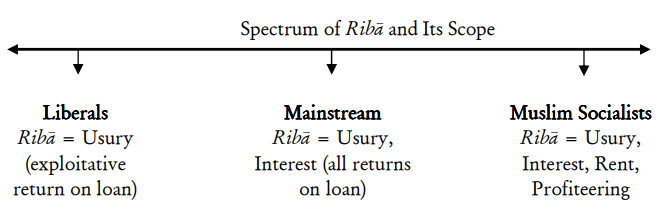
\includegraphics[width=\textwidth]{CourantsIslamContemporain/ImagesCourantsIslamContemporain/Riba.png}



The above differences have left scholars divided on several important questions that demand straightforward answers. Those questions include the following ones:
\begin{itemize}
    \item 
1. Is bank interest prohibited in the light of the Qur'an and the sunnah? If yes, how?
    \item 
2. Whether the Qur'anic term riba includes all kinds of interest rates or it relates only to the excessive interest rates?
    \item 
3. Whether the scope of riba extends to the interest charged and paid on business transactions in the banking system or is restricted to the interest charged on consumption loans only?
    \item 
4. Does Islam allow loan transactions? If yes, how and in what form?
    \item 
5. Is paying interest a lesser evil as compared to charging it?
    \item 
6. Is borrower always \textit{mazlum} (a losing party) in an interest bearing loan transaction?
    \item 
7. Does Islam allow indexation of loans on the grounds of inflation?
    \item 
8. Is credit-sale with higher deferred price as compared to the spot price allowed?
    \item 
9. Does Islam approve of “time value of money,” especially when charging higher deferred price is allowed in a credit sale?
    \item 
10. Are future currency contracts permissible in Islam?
    \item 
11. How and to what extent is salam transaction permissible?
\end{itemize}


These are but a few questions.
\begin{Synthesis}
We show in this paper that whatever confusion prevails among contemporary scholars on this subject is the outcome of following an inadequate methodology for determining the meaning and scope of riba.
\end{Synthesis}
 In fact, this methodology has mystified the nature of riba, which is otherwise clear when viewed from the methodological view point of the eminent Muslim jurists of the past. The mystification is such that not only it results in confusing answers to these questions but it also begets confusing questions. Unfortunately, the confusion has built up to the extent that the Federal Shariat Court of Pakistan has been struggling to come up with a definition of riba. It is in this background that this paper attempts to explain:

(1) the contemporary Islamic economists' methodology of interpreting and classifying riba; (2) why this methodology is wrong and insufficient; (3) the methodology of understanding riba on the pattern of Muslim jurists of the past; (4) that the methodology given by the Muslim jurists is coherent and compact.

The reader will encounter a number of arguments in this paper that are advanced by those who justify bank interest. Since the paper deals with the legal substance and not with the economic merits of arguments, hence we will restrict ourselves to the legal analysis of those arguments and leave aside their economic analysis and rationale, which require an altogether different methodology. Any legal system has three aspects: (1) what: the legal rulings (i.e., ahkam); (2) how: the rules of deriving those legal rulings (i.e., usul al-fiqh); and (3) why: the underlying rationale(s) and wisdom behind the legal rulings (i.e., hikmah)

It is important not to mix these aspects. The present study deals with the first two aspects of the issue of riba. Moreover, the classification of riba discussed in this paper is primarily based on the methodology of Hanafi jurists for ensuring analytical consistency. We presume that a school of law represents an internally coherent system of interpretation and that mixing up the views of the various schools results in inconsistencies.7 However, views of the other schools have been briefly mentioned in the footnotes wherever required. Finally, the paper does not attempt to show that the Hanafi jurists' approach is superior to all others, rather it explains that the classical jurists' approach (whether Hanafi, Maliki, Shafi‘i or Hanbali) to understanding riba is superior to that of the modern scholars. The methodology of these jurists share several common results that are important in order to answer the above questions.

Following section outlines the method adopted by modern Muslim scholars and economists. The next section discusses problems in this methodology and develops the skeleton for the methodology that is then applied in the coming section, which details out the general rules of riba alongside their resulting implications. The last section concludes the paper by giving a comprehensive definition of riba based on discussions in sections three and four.


\newpage
\subsection{Outline of the Mystifying Methodology}

Imran Ahsan Khan Nyazee\sn{\href{https://en.wikipedia.org/wiki/Imran_Ahsan_Khan_Nyazee}{Pakistan} Nyazee's academic career was inspired by the work of Abdur Rahim. Nyazee argues firstly, that due to its unique set of principles of interpretation, each school of Islamic law represents a theory of law unto itself. Secondly, he points out that Istiḥsān cannot be understood without understanding of the workings of qiyās. It is, therefore, difficult to accept that there was no system of interpretation before al-Shāfi‘ī's time. Thirdly, he concludes that the uṣūl al-fiqh never existed. Furthermore, Nyazee describes beyond the individual fikh of each school of law, another theory of interpretation called maqāṣid al-sharī‘ah (theory for the purpose of the sharī‘ah) which was developed by al-Ghazālī. Nyazee has written and self-published on a number of aspects of Islamic law. He agrees with most Muslim scholars that strictly speaking, selling money (taking interest) is prohibited, according to Islamic law. Some point out a difference between the treatment of riba in the Qur'an versus the Sunnah but Nyazee the two approaches are actually one and the same.Nyazee also proposes that all loans (except those of a charitable nature without a fixed period of repayment) and therefore all banking is prohibited and unIslamic. Nyazee is equally intolerant of murabaha, the Islamic system of business where in-put costs and mark-ups are made transparent between vendor and buyer. He argues riba will inevitably enter such transactions.[10] He extends the prohibition to the creation of wealth on the basis of debt and the fractional reserve banking system. These elements along with zakat (the system of alms-giving) he says, are the differences between Islam and capitalism. He advocates the use of the gold and silver dinars and dirhams as the currency of the Muslim community. Nyazee would also prohibit the corporation or 'legal personality' under Islamic law.} explains that the methodology adopted by modern scholars for determining the meaning of riba is the same, though they disagree in their conclusion regarding whether or not bank interest is riba.8 The fundamental problem of their methodology lies in overlooking the inherent link between the Qur'an and sunnah. This methodology of interpreting riba was initiated by Muhammad Rashid Rida (d. 1935) \sn{voir p. \pageref{Theol:Rida} Frère musulman pas le voyage en Europe. Plue el manar un commentaire coranique, sensé être l'héritage d'abdu}, which goes as follows:9

\paragraph{Lecture de Rida El Manar}
Riba is classified into two categories, riba of the Qur'an (also equated with riba 'l-nasi'ah, i.e., interest on loan transaction) and riba of hadith (equated with riba 'l-fadl, i.e., interest on exchange transaction).

Rida begins with literal meaning of the word riba (excess) and then traces some riba-based transactions practiced by Arabs during the time of Prophet (peace be on him). Rida, relying on some commentators of the Qur'an, asserts that the Qur'anic verse regarding riba deals with a specific practice of Arabs known as credit-sale where the payment of price is deferred to a future period while delivery of goods takes place on spot. Because a seller is allowed to charge whatever price he wants in a sale transaction, no riba is involved in the original price negotiated between the two parties-any excess in future price becomes part of the price. However, they used to increase the price excessively whenever the debtor would be unable to settle his debt obligations at the end of payment period. The debtor was given the option, “Will you pay the debt or increase the amount in lieu of delay?”

For Rida, it was this excessive rate (doubling and multiplying) of interest in debt-based transactions added to the original sum at the end of payment period which was prohibited by the Qur'an (he called it riba 'l-jahiliyyah).10 From this, he concluded that the bank interest is not the same riba that was deemed impermissible by the Qur'an because (a) it is neither doubling and redoubling of rates (b) nor the excess is stipulated in the initial period of the banking transaction-he assumes that the initially added interest is part of the principal or original sum just like the original sum in case of credit-sale. 
\begin{Synthesis}
Hence, for Rida, only compound interest is prohibited.
\end{Synthesis} 

Other scholars, supporting Rida's view, added that business loans were not common among Arabs as theirs was a subsistence economy; loans were largely taken by poor people for consumption purposes on interest and whenever they were unable to repay them at due time, excessive interests were added to the original sum. Hence, it was this type of interest that was declared prohibited by the Qur'an and it has nothing to do with the modern commercial loans, \textbf{which are mutually beneficial for both parties.}11

Having ascribed this meaning to the Qur'anic word riba on the basis of some historical traces, Rida then explains the form of riba declared impermissible in the sunnah as a distinct prohibition from that of the Qur'an.
\begin{Def}[Riba] Usure, profit ou gain réalisé sur un prêt.
\end{Def}

\begin{Def}
[Riba al-buyu] : Usure. Opération de vente dans laquelle une matière première est échangée contre la même matière première mais en quantité différente et la livraison d’une des matières premières est postposée. Pour éviter le riba al-buyu, les matières premières échangées par les deux parties devraient être en quantités égales et l’échange devrait être instantané. Riba al-buyua a été condamné par le Prophète Muhammad afin d’éviter que le riba (intérêt) n’affecte insidieusement l’économie.
\end{Def}
\begin{Def}[Riba al-duyun] : Usure d’une dette.
\end{Def}
 
\begin{Def}[Riba al-fadl] : La différence de quantité entre deux biens échangés et comportant du riba.
\end{Def}
\begin{Def}[Riba al-nasiah] : La différence de paiement liée au report de deux biens comportant du riba
\end{Def}\mn{cf Glossaire des termes financiers  Islamiques \href{https://www.cairn.info/la-banque-et-la-finance-islamiques--9782804167042.htm}{Banque et finance islamique} } He calls it \textit{riba 'l-fadl} which emerges in the exchange of two counter values of the same or different species and hence also called \textit{riba 'l-buyu‘}.12 The position of Rida, which may be termed as minority view, is summarised in figure 2.


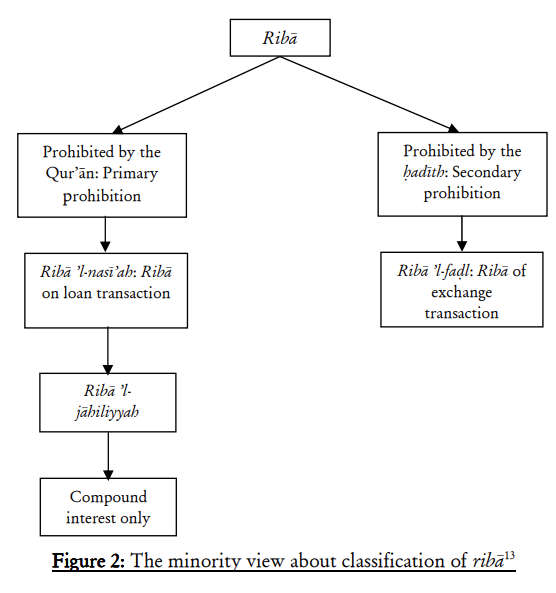
\includegraphics[width=\textwidth]{CourantsIslamContemporain/ImagesCourantsIslamContemporain/RibaRida.png}

Thus, Rida dichotomised the two concepts of riba, one attributed to the Qur'an and another to the sunnah. He finally declared the first one as real or explicit riba while latter as lighter or implicit riba.
\textbf{
Though the majority of contemporary scholars did not agree with the conclusion drawn by Rida about legitimacy of bank interest, however they adopted his methodology of classifying riba. The only difference in their opinion is that riba of the Qur'an includes all rates of return on loan and it is not merely restricted to the compound interest of jahiliyyah}\sn{la période pre islamique}


To them, business loans were a part of Arab's economy and any contractual return to lender is unfair because this is tantamount to refusing to share business risk with the borrower. We can depict their views in figure three.
\begin{Synthesis}
On a donc un nouveau problème, le pret commercial lié avec l'industrie et face à ce nouveau problème, une lecture de Rida qui est assez positive (Riba = Excess) mais qui note une différence entre Coran et Sunna) et fait une distinction entre les deux, reprises ensuite par les autres légistes, mais en repartant d'une lecture stricte du Riba comme intérêt. Il conveint d'articulier Coran et Sunna de façon non parallèle mais l'un par l'autre.
Il convient de montrer l'évolution du prêt commercial au XIX
\end{Synthesis}
Because the sunnah is not linked with the Qur'an in this methodology, both the minority and majority Muslim economists have struggled to explain as to why someone would engage in exchange transactions of the forms mentioned in hadith. Some opined that these transactions are declared impermissible because they may open the path for the “real riba” (i.e., riba of the Qur'an).


14 Others assumed that it was meant to discourage the practice of barter exchange and promote market exchange through a medium of exchange.15 Yet another view argues that it eliminates the possibility of benefiting from asymmetric information of the contracting parties.16 The truth is that none of these explanations makes the point.

2.1. The Nature of Debate within Minority and Majority Schools

The debate that has taken place within the followers of this mystifying methodology on the issue of why or why not bank interest is riba may briefly be summarised here. As explained above, Rida asserted that bank interest was not included in the Qur'anic concept of riba of debt because it was different from the riba that was charged by Arabs on credit-sale transaction by doubling and multiplying the price whenever the debtor was unable to settle his debt at due time and asked for relaxation in payment period.18 Rida explained that the Qur'anic verse “Allah has permitted bay‘ and prohibited riba”19 referred to this riba. To strengthen his case, he argued from the verse: “O Believers! Do not devour riba doubled and multiplied and fear God so that you may prosper.”20

This verse complements the former verse in the sense that what was implicit in the first verse was made explicit in the latter-both verses referred to the practice of doubling and multiplying of interest and none of them forbad the bank interest.

How do the majority of scholars respond to this argument? For example Usmani notes the Qur'anic verse:

O you believers! Fear God and give up riba that remains outstanding if you are true believers. Behold! If you do not obey this commandment, then God declares war against you from Himself and from His Prophet. But, if you repent (from riba), then you are entitled to only your principal amounts. Neither should you inflict harm to others, nor others should do harm to you.21

The argument is based on the emphasised words ‘you are entitled to only your principal amounts (ra's al-mal)'. He infers from these words that the rightful entitlement of lenders is the original sum advanced; he cannot charge any increase whether small or large (doubled and tripled). To him, the verse (3:130) forbids a severe form of riba where interest is multiplied, but it does not restrict riba to this specific form. Hence, bank interest falls within the purview of the Qur'anic verse “Allah has permitted bay‘ and prohibited riba.”22 They are also of the view that charging interest on commercial loans was also practiced by Arabs.23

Does the above analysis of mainstream scholars guarantee the prohibition of bank interest? We are afraid it does not. Their arguments rest on two assumptions:

(1) The verses (2:278-79) address the issue of loan-transaction.

(2) Ra's al-mal (principal amount) can only refer to the original principal advanced in loan.

Both of these assumptions are problematic. Following submissions can be made against them:

(a) If the meaning of the verse is to be determined with reference to historical practices, one can equally claim, just like Rida, that the verse is not about loan transaction but about credit sale. In that case, ra's al-mal is not referring to the principal amount lent; rather, it is the deferred future price of the goods sold. On which legal grounds or facts can this claim be dismissed?

(b) Further, this deferred price might include increase over and above spot price. Hence, the future price could consist of two components: spot price plus some additional profit. The sum of these two would constitute ra's al-mal (principal amount) in this transaction (i.e., principal amount in credit sale (ra's al-mal) = spot price + extra profit)

Whenever a debtor was unable to repay full amount, further multiplied increase was added to this original sum, Rida called it interest. This would increase the due amount to: total amount after increase added due to delay, which is interest in addition to ra's al-mal.

Using this structure, one can then argue that the initially added interest in a loan transaction is equivalent to initially added “extra profit,” which becomes part of ra's al-mal. Therefore, entitlement to the ra's al-mal means entitlement to the simple interest, as claimed by Rida.

(a) The only legal justification for ascertaining that the verse is about loan transaction is based on the words “ra's al-mal” (principal amount). But how can it be settled that ra's al-mal here means ra's al-mal of a loan transaction? This question is important because a number of transactions constitute a component of ra's al-mal. For example, there is ra's al-mal both in mudarabah and musharakah contracts. How to exclude these forms of ra's al-mal from the purview of the Qur'anic verse? If someone says, “This verse is about loan, so ra's al-mal refers to that of loan contract and not of mudarabah and musharakah,” he is clearly arguing in circularity. The argument goes like this:

Q: How do we know that the verse is about loan contract?

A: Because the verse talks about ra's al-mal.

Q: How do we know that ra's al-mal here refers to that of loan?

A: Because the verse is about loan contract!

A circular argument is no argument.

(b) Muslim Socialists could maintain that ra's al-mal means principal amount of all business contracts. Therefore, it is not legitimate to charge any excess over and above principal amount, no matter it is mudarabah, musharakah or ijarah.

Not only that the analysis of mainstream scholars does not necessarily imply the prohibition of bank interest, it leads to a set of unsettling arguments that have left Islamic economists bewildering about some basic issues. For example,

(1) Even if it is agreed that ra's al-mal means principal amount of a loan transaction, does it mean “nominal” amount or the “real” (inflation adjusted) amount? Again, what are the legal grounds to settle this issue? Because there are no clear-cut legal grounds available in this methodology, we see scholars are divided on this subject matter-some allow indexation of loan against inflations while others do not.

(2) What about the question of “time value of money?” This question poses challenge for Islamic economists because they, as a rule, approve the practice of charging higher price in credit-sale and murabahah.

(3) The Lawgiver has allowed salam, what are the legal grounds for not extending this permission to currency salam (future currency contracts)?

Undoubtedly, majority view has addressed these issues, but the answers do not seem to be stemming out of a coherent analytical legal system. This approach is often found mixing up legal analysis with economic analysis. This missing coherent analytical legal system is the root cause of most of the mystification that has prevailed all over. It is an unfortunate state of affairs and it is high time to demystify things.

3. Methodological Assumptions of Premodern Muslim Jurists (Fuqaha') for Understanding Riba

To understand the method used by the eminent premodern Muslim jurists for understanding riba, three methodological issues (MI) need to be clarified. They are explained by Nyazee in detail.24

1) Link between the Qur'an and Sunnah

The methodology adopted by the modern Muslim scholars and economists is misleading because it delinks the Qur'an and sunnah. It assumes that the meaning of riba is different in the Qur'an and sunnah, which is not the case. To explain the nature of error made by both the groups, it should be noted that Muslim jurists (fuqaha') classified riba in the category known as mujmal (unelaborated)25 whose meaning and scope cannot be determined without explanation (bayan) of the Lawgiver (Shari‘). The famous hadith (as given in footnote 1) that explains different usurious transactions actually does not add something to the Qur'anic word riba. Rather, it defines its meaning and scope.

Thus, while to the contemporary scholars the meaning of riba is known independent of hadith and they see hadith as adding some more cases to the Qur'anic concept of riba, the jurists say that hadith is the definition of the term riba used by the Qur'an. Thus, riba 'l-nasi'ah and riba 'l-fadl both are included in the Qur'anic concept of riba.

2) Relationship between Loan and Bay‘ (Exchange)

Loan is also classified as a form of exchange transaction (bay‘)26 by Muslim jurists. The scope of this paper does not allow detailed analysis of this assertion.27 For descriptive purposes, it can be seen that a loan of Rs X is an exchange of Rs X today with Rs X after time deferment (and with Rs X + Y if interest payment of Rs Y is included). Figure 4 depicts this nature of loan transaction by illustrating a loan transaction between Mr. A and B:

3) Skeleton of a Coherent Legal System

A coherent shari‘ah-based legal system consists of a set of general rules, called

‘azimah by the jurists, supplemented by some exemptions to these laws, called rukhsah. In the words of Nyazee, ‘Azimah (lit. determination, resolution) is applied to mean a rule that is applied initially and for itself. Such rules form the backbone of the law. As against this, there may be a rule that goes contrary to the requirements of the initial rule, but is permitted by the law. This rule is considered to be a rukhsah (exemption) from the initial rule.28

This classification of ‘azimah (the higher or first order rules) and rukhsah (the lower or second order rules) is important for several reasons.

First, it explains the order in which the rules have to be applied.

Second, it explains why sometimes two opposing cases may be allowed within a given skeleton of law.

Third, the order of rules implies that an exception cannot be extended using any method of argument, whether analytical or analogical. On the other hand, extension of first order rules is legitimate by these methods. In other words, it is not allowed to build a sub-legal system based on exemptions because otherwise it starts negating the primary provisions and objectives of the law-an exemption from the general rule must remain an exemption.

Fourth, because of the logical hierarchy in the operations of ‘azimah and rukhsah, it is clear that an exemption from a rule cannot be used to nullify or change the shari‘ah status (hukm) of any other case that is derived from the general rules. Alternatively put, an exemption (a lower order rule) cannot prevail over the higher order rules.

Fifth, because all rules and exemptions are derived from nusus (the Qur'an and sunnah), hence the only justifiable exemptions are the ones, which are given in nusus (i.e., stated by the Lawgiver Himself).

We call these nusus the “facts” of the shari‘ah-based legal system in this paper. Given these “legal facts,” the task of a jurist is to derive those general rules (‘azimah) from the facts, which render these facts internally consistent and extendible on the one hand and highlight the exemptions (rukhsah), if any, on the other.29 Finally, the general rules and exemptions generate some implications, called ahkam. This skeleton of a shari‘ah-based legal system is illustrated in Figure 5. We apply this skeleton in this paper to elaborate riba.

The relevant “legal facts” used by premodern Muslim jurists to derive general rules and exemptions are quoted at the relevant places in this article. We are now in a position to take on the issue of derivation of the general rules and the implications from those “facts.”

4. Underlying Rules behind the System of Bay‘ in Jurists' Methodology

Our intention in this paper is to reveal that the apparently large and complicated system of legal injunctions (ahkam) is reducible to a few set of rules derived from fewer legal facts. We propose that a majority of ahkam (legal injunctions or provisions) governing economic transactions (buyu‘) can be derived from three broad rules:

1. Rules of riba mentioned in the sunnah. This is not a single rule, rather a set of rules as explained below.

2. Rule about the sale of goods not possessed by a person.

3. Rule about exemption that an exemption is to be treated as exemption.

Before explaining these rules, we first explain the context of the Qur'anic verses that underlies the jurists' methodology of riba to clarify the misconception that the relevant verses of Surat al-Baqarah are about loan transaction and not exchange (bay‘).

4.1. The Context of the Verses of Surat al-Baqarah

The Qur'an states that the disbelievers said, “Verily, bay‘ (sale) is just like riba.” In response to this, it was said, “Allah has permitted bay‘ and prohibited riba.” To understand why the disbelievers said this, consider these three transactions:

(a) A gives B 100 grams of gold in exchange of 110 grams of gold to be paid after one year. This is primarily a sale contract as explained previously (i.e., exchange of 100 grams gold with 110 grams gold with time lag) and involves riba (how, this will be explained in the next section but take it for granted for the moment).

(b) A asks B for 100 grams of gold in exchange of, say, 500 kg wheat at spot. This is a legitimate regular sale contract.

(c) A demands from B 110 grams of gold in exchange of 500 kg wheat for payment of price after one year: this is credit sale contract with higher deferred price as compared to spot price and is also legitimate (this is explained in section 4.3).

The credit sale was a common practice among Arabs and, therefore, they were confused as to why the transaction (a) is impermissible and (c) is permissible while the two are quite similar in nature (i.e., both are credit sales and both involve access payment). In (a), 10 grams of additional gold are paid as counter-value for 100 grams of gold for a delay of one year and similarly 10 grams of gold are paid for a delay of one year in transaction (c). It is for this reason that disbelievers said, “Verily sale is just like riba!” That is, transaction (c) (i.e., the credit sale) is similar to the transaction (a). The technical reason for allowing transaction (c) and forbidding (a) is the similarity of genus which is explained by the sunnah. This is explained in the next sections in detail, but the important point to note here is that the assumption that the Qur'anic term riba is not about sale contract, rather it is about debt, is not implied by these verses.

Thus, the verse says that Allah has approved all forms of buyu‘ (exchange transactions) except those which involve riba.30 The natural question then arises: what is this thing called riba? Has the Qur'an given any definitive description of riba?

One may make one of the two assumptions here. First, the concept of riba was largely a sort of common knowledge for everyone and, hence, it required no legal description by the Qur'an. That common knowledge is traceable by an examination of historical record of Arabs which provides sufficient legal foundations for determining the meaning of riba. As far as the details of riba in the sunnah are concerned, they were additions over and above to that common knowledge of riba and most of these additions were unknown to the Arabs. The liberals and mainstream scholars share this assumption and we believe that this assumption constitutes what we called the “mystifying methodology.”

Second, some forms of riba may be or actually known to the Arabs but these do not set the legal standard against which the Qur'anic concept of riba is to be determined. As it is a legal term, its meaning has to be sought from the Lawgiver. In technical sense, the jurists call it mujmal (unelaborated) for which elaboration (bayan) is sought from the Lawgiver. This elaboration of the legal meaning of the Qur'anic term riba is given by the sunnah. After this elaboration by the Lawgiver, its meaning is determined definitively and it becomes mufassar (elaborated). This is the methodological assumption that the jurists use not only for defining riba but also for other legal terms of the Qur'an, such as salah, zakah, and so on.31 Thus, according to this second assumption, the practices and concepts of Arabs may be referred by the Qur'anic concept riba but it is not the benchmark against which we assign legal meaning to the Qur'anic terms.

For example, the Arabs had some concepts about how to offer salah (prayer), but this information does not define the legal meaning of the Qur'anic term salah nor is this concept limited to this information set. Similar is the case with riba. The Arabs might have been aware of some forms and practices of riba but that does not constitute the legal definition of riba. When the jurists classify a term as mujmal, they mean that this term is a technical legal term and its meaning should be determined with reference to the words of Lawgiver Himself, neither by the linguistics (dictionary) nor by the historically known social concepts and practices that hover around that technical term. It should be emphasised here that considering riba as mujmal does not mean that the Arabs did not know the meaning of this word at all. Nor does it mean that the pre-Islam Arabs did not identify certain transactions as riba-in fact they did and the jurists did consider it part of riba.32

It only means that the meaning of riba in Islamic law is not limited to, and is not based on its usage in the pre-Islam Arabia. The Qur'an and the sunnah added several shades of meaning to this concept. That is why, it became a “technical term” of Islamic law. Hence, its meaning and scope cannot be determined by its dictionary meaning or its practice and understanding by the pre-Islam Arabs. Rather, it must be determined by the Qur'an and the sunnah, like any other legal term such as salah and zakah. Just as we cannot classify concept salah as salah of the Qur'an and salah of hadith, similarly we cannot dichotomise riba. Once it is established that the meaning of riba must not be gathered from pre-Islamic usage and practices but from the Qur'an and the sunnah, the next question is: how to explain the various usages of riba in the Qur'an and the sunnah? The answer, as per the well-established methodology of the jurists, is to consider the sunnah as the elaboration of the mujmal verses of the Qur'an.

This methodology is employed by the jurists for determining the meaning and scope of salah and zakah as well as riba. Let's follow through the path of righteous ones here and have its blessings.

4.2. General Rules of Riba When Transacted Species are Same

Keeping these in mind, one has to understand the classification of riba in the system of Muslim jurists. Because the sunnah defines riba, note the words of hadith,

When you exchange gold for gold, silver for silver, wheat for wheat, rice for rice, dates for dates, and barely for barely, then exchange like for like (in equal measure) and exchange them hand to hand (at spot), else it will be riba.33

To understand what it says, consider these transactions:

1) exchange of 1 gram gold for 1 gram gold on spot;

2) exchange of 1 gram gold for 2 grams gold on spot;

3) exchange of 1 gram gold at spot for 1 gram gold with delay;

4) exchange of 1 gram gold at spot for 2 grams gold with delay.34

As per the hadith, the first transaction is allowed; the second one is disallowed because it involves excess in measurement/quantity (called riba 'l-fadl); the third transaction is also impermissible because the hadith says that the exchange of homogeneous goods is allowed in equal measurement provided it is on spot; therefore, this transaction involves the riba 'l-nasi'ah (i.e., riba of delaying); finally, the fourth transaction involves both types of riba. These transactions provide two guiding rules (R):

R 1.1) Goods of the same species cannot be exchanged immediately unless their measurement (in terms of weight or volume) is same.

R 1.2) Goods of the same species cannot be exchanged with time lag, even with same measurement.

4.2.1. Implications

Five important implications (I) should be noted.

I. 1) Impermissibility of Market for Loanable Funds

Application of rule 1.2 gives the important implication that loan, with or without interest, is prohibited in Islam because, as explained above, a loan is an exchange of homogeneous goods with time lag. Does it mean that loaning is not allowed in Islam under any circumstances? Of course, this implication of the general rule is at odd with a number of legal facts (nusus), which promise reward for offering loan to the needy ones. How to reconcile these apparently contradictory legal facts now? This is where the concept of rukhsah (exemption) is activated by the jurists. Though loaning is against the general rule (‘azimah) given by the Lawgiver, yet it is allowed by Him as an exemption from this prohibition if it takes the form of benevolent giving (tabarru‘ or sadaqah).35 Loan is classified as tabarru‘ if:

(a) it is out of the intention of benevolence to the other person (i.e., the lender consciously bestows upon the borrower the benefits associated with his asset);36

(b) no increase in its value is stipulated, else it would cease to be benevolent and would involve riba 'l-fadl; and

(c) no contractual time limit is stipulated, the lender can ask for his asset anytime he wants.37 Stipulating (legal) time constraint in loaning activity makes it a business transaction as per the application of general rules of shari‘ah and, hence, unlawful because in that case it is simply the exchange of homogeneous goods with time delay, which is not allowed, whether or not interest factor is included. Moreover, making the time period binding would imply that the lender is forced to do, or to continue with, an act of charity. This is against the very nature of charity.

In short, this principle implies that Islamic law does not permit the “market for loanable funds.” It sees loaning as an act of benevolence, especially in favour of one's relatives.38 Stated alternatively, loan is purely a social transaction (a means of tying and strengthening social bonds) in Islam and not a business. It was in this social transaction capacity that the institution of loan prevailed for thousands of centuries not only in Muslim societies but also in other civilisations of the world until the emergence of capitalism in the fifteenth century.39 Note that this important result (impermissibility of the market for loanable funds) does not follow directly from the classification of modern scholars of Islamic economics, as the majority view allows interest-free non-benevolent loans as a general rule and not as an exemption.

This implication answers one of the important arguments in favour of bank interest given by some economists. The argument says that interest should be allowed in shari‘ah because interest is the price of capital and without interest the market for loanable funds cannot be equilibrated. Because we are not dealing with the economic merit of arguments in this paper, we ignore its economic substance and comment on its legal merit only. It is clear from the above implication now that this argument has no shari‘ah basis because shari‘ah does not allow market for loanable funds to begin with, let alone equilibrating it from shari‘ah perspective.

Before moving on to the next implication, the important implication and exemption regarding loan transactions be noted:

I 1.1) A loan transaction is prohibited, whether or not interest factor is added to it.

I 1.2) A benevolent interest-free loan is recommended as an exemption to the general rules of riba by the Lawgiver.

I. 2) Impermissibility of Bank Interest

All forms of bank interest, whether simple or compound, are prohibited by Islam as per Rules 1.1 and 1.2. Similarly, the fact whether loan is made for business or consumption purposes makes no difference to this result. There remains no confusion about these conclusions if the shari‘ah rules are applied with consistency. In fact, the practice of charging interest by the bank includes both kinds of riba and it, therefore, may be stated that it is the most comprehensive form of riba! This can be verified from the figure 6, which depicts detailed structure of riba-based transactions in case of homogenous goods (leaves aside heterogeneous goods for the moment).

I. 3) False Dichotomy between “Giving and Taking” Riba

The recipient of riba is not always the lending party as is usually perceived. It can be seen from above examples that in case of transaction (2) the lender is the beneficiary of riba, but in transaction (3) riba is received by the borrower, and finally both are its recipients in transaction (4). Hence, opinions such as “taking riba is a greater evil than giving it and, hence, paying interest to the bank is a lesser evil” are based on the fallacious assumption that it is only the bank that receives interest in a typical interest-bearing loan transaction. This wrong assumption is the outcome of using the wrong methodology outlined in section two.40

I. 4) Mutually Beneficial Riba is Prohibited

The view that bank interest realised in transaction (4) is or should be permitted (as claimed by liberal Muslim scholars) is implicitly based on the assumption that “two wrongs make one right”-that is, it assumes that mutually enjoyed riba of the lender and borrower can make this transaction acceptable while the matter of fact is that each of them is separately prohibited to begin with.

I. 5) Irrelevance of Time Value of Money

Following the wrong methodology has resulted in another confusing argument that the bank interest should be allowed because of “time value of money.” This argument is based on the presumption that Rs. 1 today is worthier than Rs. 1 tomorrow. Why? Economists believe that this is due to the subjective time preferences of an individual. A rational (i.e., self-interested utility maximising) economic agent is said to have positive time preferences in the sense that consumption today is preferred to consumption tomorrow because the latter is uncertain, which makes him impatient, thus he wants to have it today than tomorrow.

Another reason for having this positive time preference emerges from the institutional arrangements: if I have the option of earning some interest (say Rs. Y) on Rs. 1 by putting it in a bank account today, why should I lend it to someone for free? Putting Rs. 1 in a bank account will make it “Rs. 1 + Rs. Y” for sure (assuming away bank insolvency), say, after one year while lending it to someone will leave it worth Rs. 1. Hence, Rs. Y (which may be expressed in percentage) is the price that should be paid to the lender for a loan of one year, else it would be unfair with him. This argument is more of economic than legal in its substance, however, some comments can be made here to evaluate its legal substance in the light of preceding discussion.

The relevant part of the proposed argument is the second one (the institutional arrangement) because the first one is merely a subjective feeling, which may differ from person to person (as a matter of fact, not everyone prefers to consume more today than tomorrow). The argument presumes that there exists and should exist a well-established legally functional market for loan, which coordinates interest-based loan transactions. But just recall “I.1” that Islam does not approve of the market for loan to begin with. Eliminate this institution of market for loan, and the argument disappears. The point is that the concept of “time value of money” conceived in this economic sense is alien to the discussion of riba. Its validity presumes that there exists a legal institutional market for loanable funds where money is growing continually and, therefore, an individual always has the option of putting his money in that market.

Not only that this assumption is invalid from the point of general rules of shari‘ah as explained, it is also in contradiction with the ontological structure of the universe and economic facts.

The above is not the only format of this argument, it is phrased in some other shades as well. For example, it is stated that money could buy benefits and had the lender not lent it he could have benefitted himself. This implies that lending is an act of sacrificing the benefits associated with money. Therefore, the lender should be compensated for this sacrifice and interest payment is exactly that reward. This reward makes sense given that the borrower takes benefit out of money. The argument is valid to the point that money is beneficial to the lender and that if he makes the choice of not lending it, he can benefit from it. Moreover, it is also true that the borrower enjoys the benefits associated with the money. None of these facts is denied by the shari‘ah rules. But these facts alone cannot formulate the required case for this argument; it requires a moral statement in its premise to derive the desired conclusion.

To see this, note that the argument does not end here, after quoting these facts it then makes a moral assertion: “it is morally (and hence legally) right if money is lent for reciprocal benefits.” Addition of this moral statement is necessary for validating the conclusion that “interest is the just reward for lending.” But this moral assumption contradicts the general rules of the shari‘ah, which are laid down above. Seeking reciprocity in loan is exactly what that changes its status from tabarru‘ to loan as a business transaction and, hence, it becomes nothing but riba. The argument here is quite straightforward:

The owner of money is granted the right of benefitting from his money by shari‘ah rules; he is given the option of making a conscious choice of transferring the benefits associated with his money to another person as an exception to the general rules by the shari‘ah, but there is neither any general rule nor any exemption from the Lawgiver that assigns him the right of lending money in the name of the so-called “mutual benefits” (refer to I. 4 above). Legally speaking, this involves both riba 'l-fadl (because the homogeneous goods are exchanged at different rates) and riba 'l-nasi'ah (because time stipulation is invoked-the lender asks for the excess of measurement for parting with the benefits of his money for a specified time).

Another variant of this argument comes with the heading of “effects of inflation on money.” We deal with it in the next section.

4.3. General Rules of Riba when Transacted Species are Different

What about the exchange of heterogeneous goods? The last words of the hadith are as follows: “If these species differ, then exchange as you like as long as it is from hands to hand.”

They give an immediate rule:

R 1.3) Goods of the different species can be exchanged with difference in measurement.

This rule says that such goods can be exchanged at different rates as far as measurement is concerned. In other words, riba 'l-fadl does not apply in case of heterogeneous goods. Is riba 'l-nasi'ah (prohibition of time delay in payment) also not applicable in this case? Apparently, it seems that it is not because of the words of hadith, “exchange should be on spot.” This has an odd implication that credit sale (sale of goods against money where payment is deferred to future time period) is not permissible under the shari‘ah rules. This is so because credit-sale is an exchange of heterogeneous goods with time lag. But the legal facts reveal that the Lawgiver has allowed credit-sale.41 How to explain this? Is credit sale also an exemption to the general rule, like a loan transaction? The answer is: “No, it falls within the general rules.”

To see how credit-sale is permissible within general rules, one needs to dig deep into the issue of the underlying cause (‘illah) that the Muslim jurists derived from the sunnah to understand the system of riba. The relevant question facing jurists was: Is prohibition of riba restricted only to the six goods named in the hadith or is it extendible to other goods? The answer of the jurists is, yes, it is extendible and for this extension they derived the underlying cause due to which riba was declared prohibited by the Lawgiver. Keeping aside the technical details and arguments, it should be noted that some of the goods are measured in terms of weight while others are measured in terms of volume. In the hadith under discussion, gold and silver were weighable while the other four items were volumeable at the time of Prophet (peace be on him).42 Based on this classification, the jurists derived two further rules:

R 1.4) when species are different but their method of estimation is the same (such as gold vs silver or wheat vs rice), unequal quantities can be exchanged, provided that the exchange is immediate;

R 1.5) when species are different and their method of estimation is also different (such as gold vs wheat), unequal quantities can be exchanged with time delay.43

Thus, the credit sale is allowed due to the application of Rule 1.5. To see this, consider these combinations of transactions:

1) Exchange of 1 gram gold at spot for 2 gram silver on spot (method of estimation same)

2) Exchange of 1 gram gold at spot for 2 gram silver in future (method of estimation same)

3) Exchange of 2 kg wheat at spot for 1 gram gold/silver on spot (method of estimation different)

4) Exchange of 2 kg wheat at spot for 1 gram gold/silver in future (method of estimation different)

The first transaction is allowed but the second is not because when species are measured by same method (i.e., “weight” in this case), then difference in the measurement (fadl) is allowed but deferment (nasi'ah) is not permissible. The third and the fourth transactions are allowed because here not only the transacted species are different but also their method of measurement (one was measured in “weight” while the other in “volume”).

In short, when both of the similarity factors (i.e., species and method of measurement) are found, then both fadl (excess of measurement) as well as nasi'ah (excess of time delay or time deferment) are prohibited. When similarity of measurement is found alone, then fadl is allowed but nasi'ah is prohibited. Finally, when none is found, both fadl and nasi'ah are allowed. Figure 7 depicts all of these rules completely (discussion about the last layer of boxes on the right-hand side of this figure is coming next).

The preceding discussion shows that the hadith explaining the nature of riba was not about the actual practices of Arabs that begged some economic explanations with which Muslim scholars have been struggling. Rather, it stipulated the rules of exchange. It says, “If at all you make exchange transactions, here are the governing rules.” Thus, all transactions that correspond to these general rules are allowed while those in contradiction with them are prohibited (however, some are exempted by the Lawgiver).

4.3.1. Implications

Following implications are derived from the above rules. It is important to note that the first two transactions mentioned in sub-section 4.2 belong to the case when method of estimation of the heterogeneous goods is same while the latter two cover the cases when their method of estimation is different.

I. 6) Placement of Regular and Credit-Sale

Transaction (3) is categorised as regular sale transaction (usually termed bay‘) by the jurists. On the other hand, transaction (4) covers credit sale, which may take two forms: with or without extra profit margin as compared to the spot sale. Because both measurement as well as payment time differential are allowed in this case, hence credit sale of both forms is allowed.

I. 7) Placement of Currency Exchange

The remaining two boxes are relating to the exchange of currencies (termed as bay‘ al-sarf by the jurists). A detailed description of these requires an appreciation of some more technical classifications44 made by the Muslim jurists. However, they are beyond the scope of this paper. Suffice to say that the jurists divided all tradeable species into two: (a) currency items, which are used as means of exchange; they included gold and silver (though other goods may also be treated as currency in this system) and (b) non-currency items, (goods that are exchanged, and are not medium of exchange). They roughly included all but gold and silver.45 Given this division, the jurists broadly mention four types of transactions (buyu‘):

(1) Non-currency item in exchange of non-currency item-called barter exchange.

(2) Spot or delayed currency (say gold) in exchange of spot non-currency (say wheat) item.

(a) If both of them (gold and wheat) are exchanged on spot, it is called regular sale of goods, and

(b) if the currency price (gold) is delayed, this is called credit sale.

(3) Delayed non-currency item (say rice) in exchange of spot currency item (say gold). Here, the price of the good is paid on spot while its delivery is delayed. This is called bay‘ al-salam (advance payment) by the jurists.

(4) One currency (gold) in exchange of another currency (silver)-known as bay‘ al-sarf.

Rules regarding the first two have been discussed above. Here, we have to make some submissions regarding this fourth type of transaction. Because this transaction comes under the umbrella of “different species with same method of measurement,” it is clear from figure 7 that the excess of measurement is allowed in this transaction while time deferment is not. This gives two further rules under rule (1.4):

1.4a) If different currency items (such as gold and silver) are exchanged, then it is allowed to exchange them at any rate;

1.4b) if different currency items (such as gold and silver) are exchanged, then it is not allowed to exchange them with time deferment.

If it is accepted that modern currencies are just substitutes of gold and silver, then two further important results emerge from this discussion:

I 7.1) Future Currency Contracts are Prohibited

Rules (1.4a) and (1.4b) imply that the spot currency transactions are allowed while their future contracts (known as currency salam in Islamic finance literature) are prohibited in Islam as they come under the purview of riba 'l-nasi'ah.

I 7.2) Indexing of Loans is Prohibited

Indexing the value of the currency loans against some underlying assets (say gold) on the ground of inflationary pressures is not allowed. It is often argued that since the value of currency decreases over time due to the presence of inflation, hence an extra-payment equal to the rate of inflation, over and above the original sum given in loan, should be allowed in favour of the lender to keep his purchasing power. Again, because the economic merit of this argument is beyond the scope of discussion in this paper, we restrict only to its legal merit. If it is accepted that one rupee is legally nothing but equivalent of 1 unit of gold or silver (whatever that unit be), then Rules 1.1 and 1.2 (governing the loaning contract in gold or silver currencies) should automatically become operational.

Those rules imply that (a) loaning in the form of currency item is allowed if and only if equal measurement (whatever the unit of measurement) is returned; else it would be riba 'l-fadl; and (b) it is a loan made out of benevolence and not business intention (having time stipulation); else it would be riba 'l-nasi'ah. Hence, adding an extra amount to loan transaction in the name of “indexation” is but both, riba 'l-fadl (because of the excess of measurement) and riba 'l-nasi'ah (because the increase is time bound). 46 Again, let simplicity and sanity prevail.

I. 8) Placement of Salam

To see how the jurists accommodated salam in this scheme, note that there is nothing in the set of rules 1 (from 1.1. to 1.5) which forbids it. However, according to rule 2 (given at the start of this section), selling what one does not possess is not permissible and this is exactly what a salam transaction involves. Thus, a salam transaction should not be allowed as per the general rules of shari‘ah. We are once again faced with the same issue: salam is permitted in the “legal facts;” how and where to place it in the legal skeleton of the shari‘ah? Is there another general rule, which governs its permission as we saw in case of credit sale or is it an exemption from the general rule just like loan? The jurists' answer is the following: Salam is permitted as rukhsah-exemption from the general rules-by the Lawgiver.47

Because it is an exception, as per rule 3, it would be allowed only as “one of its kind” (sui generis) and cannot be used as justificatory mode for deriving more comparable transaction forms (e.g., currency salam). An exception to the general rule remains exception and does not turn into a rule for other cases because then it ceases to be an exception and creates a situation of self-contradictory general rules, which is not acceptable in any legal system. Thus, salam transaction is allowed as an exception for those transactions where (a) a currency item is exchanged against a non-currency item and (b) non-currency item is deferred while the currency-item has been paid at spot.48 This is what the exception is all about; one cannot extend this exception to the transaction types where currency items are exchanged with each other because that would violate condition (a) of the exception case.49

Figure 8 shows a map of interplay among legal facts (nusus), general rules, exemptions, and the derived implications related to riba and bay‘ that are discussed in this paper. This diagram shows that a rather complex looking system of ahkam (implications) showing up at the ending layer boxes of figure 8 emerge out of a set of general rules, which are derived to make underlying legal facts compatible with each other.

5. Conclusion: The Definition of Riba

We conclude this paper by elaborating a comprehensive definition of riba that can be inferred from the discussions in this paper. Let's quote it from al-Sarakhsi:50
\begin{Synthesis}
Riba in its literal meaning is excess... and in the technical sense (in the shari‘ah), riba is the stipulated excess without a counter-value in bay‘ (sale).51
\end{Synthesis}


Let's explain it noting several points about this definition:

(1) Muslim jurists do not introduce the word loan in the definition of riba because they categorise loan transaction under exchange (bay‘). Not appreciating this point resulted in the misconception that since the fiqh conception of riba does not deal with the subject of bank loans, it needs to be inferred directly from the Qur'an.

(2) Riba is excess, either in the form of quantity (qadr) or in the form of benefits of delay (nasa'). The first is called riba 'l-fadl while the latter is called riba 'l-nasi'ah.

(3) This excess is without any counter-value permitted by the shari‘ah. Thus, the excess of quantity paid in lieu of time delay in case of interest-bearing loan is not allowed because these two cannot be the legitimate counter-values (see I. 4).52 For a substance to be counted as counter-value, it must be recognised by the general rules of the shari‘ah to begin with.53

(4) The excess is stipulated in exchange. If the excess is granted voluntarily, it would not be riba.

We started off with specific questions in the introduction. The appendix lists down the answers to these questions in the light of the above definition of riba. It can be seen that once the discussion about riba is placed on the right track, right and clear cut answers start emerging automatically.

Appendix: Questions and their Answers that Follow from the above Analysis

Notes

1 For detailed arguments of this position, see Abu 'l-A‘la Maududi, Sud (Lahore: Islamic Publications, 2000), 110-12; M. Umer Chapra, “The Nature of Riba in Islam,” Hamdard Islamicus 7, no. 1 (1984): 3-24; Muhammad Shafi‘, Mas'alah-i Sud (Karachi: Idarat al-Ma‘arif, 1996), 43-47; Muhammad Ayub, “What is Riba? A Rejoinder” Journal of Islamic Banking and Finance 13, no. 1 (1996): 7-24; Muhammad Taqi Usmani, The Historic Judgment on Interest Delivered in the Supreme Court of Pakistan (Karachi: Idarat al-Ma‘arif, 1999), 12-16; Mohammad Nejatullah Siddiqi, Riba, Bank Interest and the Rationale of Its Prohibition (Jeddah: Islamic Research and Training Institute, 2004), 45-48; and Mahmoud A. El-Gamal, Islamic Finance: Law, Economics, and Practice (Cambridge: Cambridge University Press, 2006), 46-52. Within this category, there are further two approaches.

One approach that represents traditional ‘ulama' emphasises the resurgence of only those business contracts that were approved by the early Muslim jurists. It proposes profit-and-loss sharing (PLS) as an ideal alternative to riba. Though it does not deny the permissibility of other than PLS-based financing instruments such as murabahah and ijarah, yet it affirms that equity-based financing method is the primary means of achieving desirable economic objectives. The second approach is pragmatic one. It justifies a more liberal and flexible stance on structuring shari‘ah-compatible transaction forms that looks for financial engineering to meet all demands of modern banking customer.

2 Muhammad Rashid Rida (d. 1935) was among the foremost proponents of this theory. See his al-Riba wa 'l-Mu‘amalat fi 'l-Islam (Cairo: Dar al-Manar, 2007). Also see Sayyid Yaqub Shah, “Islam and Productive Credit,” The Islamic Review 47, no. 3 (1959): 34-37; Fazlur Rahman, “Riba and Interest,” Islamic Studies 3, no. 1 (1964): 1-43; Timur Kuran, “On the Notion of Economic Justice in Contemporary Islamic Thought,” International Journal of Middle East Studies 21, no. 2 (1989): 171-91; Izzud-Din Pal, “Pakistan and the Question of Riba,” Middle Eastern Studies 30, no. 1 (1994): 64-78; and ‘Abd al-Karim Athari, Sud Kiya Hay? (Mandi Baha' al-Din: Anjuman-i Isha‘at-i Islam, 2008), 8-12 3 Constant J. Mews and Ibrahim Abraham, “Usury and Just Compensation: Religious and Financial Ethics in Historical Perspective,” Journal of Business Ethics 72, no. 1 (2007): 1-15.

4 See Ghulam Ahmad Parvaiz, Nizam-i Rububiyyat (Lahore: Idara-i Tulu‘-i Islam, 1978).

5 Rafi‘ Allah Shihab, Kirayah-i Makanat ki Shar‘i Haithiyyat (Lahore: Kitab Ghar, 1981).

6 Ziaul Haque, “The Nature and Significance of the Midieval and Modern Interpretations of Riba,” The Pakistan Development Review 32, no. 4 (1993): 933-46.

7 For details, see Imran Ahsan Khan Nyazee, Theories of Islamic Law: The Methodology of Ijtihad (Islamabad: Islamic Research Institute, 1994), 9-12.

8 Nyazee, The Concept of Riba and Islamic Banking (Islamabad: Institute of Advanced Legal Studies, 1995), 11-19. Imran Ahsan Khan Nyazee (b. 1945) is a well-known scholar and a prolific writer on the subject of Islamic law and is a former Professor of law in International Islamic University, Islamabad. His major works include Theories of Islamic Law; Islamic Jurisprudence; Islamic Law of Business Organization; and The Concept of Riba and Islamic Banking. He also translated some of the classical texts on Islamic law and jurisprudence, including: Hidayah of Marghinani; Bidayat al-Mujtahid of Ibn Rushd; Amwal of Abu ‘Ubayd; and first two volumes of Muwafaqat of Shatibi.

9 Rida, al-Riba wa 'l-Mu‘amalat fi 'l-Islam, 69ff.

10 Period before the advent of the Prophet (peace be on him) is referred to as jahiliyyah (i.e., the period of uncivilised state of affairs).

11 Fazlur Rahman, “Riba and Interest,” 7-8.

12 In this regard, a hadith reads, “The Prophet said, ‘While exchanging gold for gold, silver for silver, wheat for wheat, barley for barley, dates for dates, and salt for salt, exchange like for like, in equal measure, and exchange from hand to hand. If these species differ, then sell as you like as long as it is from hand to hand.'” Muslim b. al-Hajjaj, Sahih, Kitab al-musaqah, Bab al-sarf wa bay‘ al-dhahab bi 'l-wariq naqdan.

13 Adopted from Nyazee, Concept of Riba.

14 Maududi, Sud, 118-19.

15 Chapra, “Nature of Riba in Islam,” 3.

16 Siddiqi, Riba, Bank Interest and the Rationale of Its Prohibition, 49-50.

17 Adopted from Nyazee, Concept of Riba.

18 Rida, al-Riba wa 'l-Mu‘amalat fi 'l-Islam, 69-70.

19 Qur'an 2:275.

20 Ibid., 3:130.

21 Ibid., 2:278-79.

22 Ibid., 2:275.

23 For details, see Shafi‘, Mas'alah-i Sud, 106-120 and Siddiqi, Riba, Bank Interest and the Rationale of Its Prohibition, 38-40.

24 Nyazee, Concept of Riba, 35-36.

25 Mujmal is a term used by Muslim jurists to refer to a Qur'anic term that begs its explanation through the words of Lawgiver (i.e., God and His Prophet [peace be on him]). One cannot interpret mujmal either by looking its meaning in the dictionary nor can its meaning be determined through historical practices at the time of revelation of the Qur'an. Mujmal can be elaborated only by the Lawgiver. Another example of mujmal is the Qur'anic term salah (prayer) which cannot be interpreted literally.

26 Bay‘ means exchange of counter values, and is not restricted to sale of goods/services. Abu Bakr b. Mas‘ud al-Kasani (d. 587/1191), the illustrious Hanafi jurist, defines bay‘ as “exchange of property with property” and then elaborates that the concept includes not only ordinary sale but also barter, exchange of currencies, advance payment and many other forms of exchange. Bada'i‘ al-Sana'i‘ fi Tartib al-Shara'i‘, ed. ‘Ali al-Mu‘awwad and ‘Adil ‘Abd al-Mawjud (Beirut: Dar al-Kutub al-‘Ilmiyyah, 1997), 6:532-33. Abu 'l-Hasan ‘Ali b. Abi Bakr al-Marghinani (d. 593/1197), author of the authoritative Hanafi manual al-Hidayah, also explicitly asserts that qard (loan) begins as an act of charity but becomes an exchange transaction in the end. al-Hidayah fi Sharh Bidayat al-Mubtadi (Beirut: Dar Ihya' al-Turath al-‘Arabi, n.d.), 3:60

27 See Nyazee, Concept of Riba, 45-46.

28 Ibid., 49.

29 The Hanafis use the methodology of istihsan (juristic preference) for ensuring harmony and analytical consistency within the law when general rules and legal facts seem to contradict. If something appears prohibited in the light of the general principles of law, but has been explicitly permitted by one of the texts (i.e., legal facts), the Hanafi jurists take the position that it is permissible as an exception to the general principle. They use the rule, “prohibited under qiyas but permissible under istihsan” for this purpose. Exceptions to the general principles are made on the basis of the text, consensus, necessity or some other “covered principle” (qiyas khafi), which needs to be uncovered. Muhammad b. Abi Sahl al-Sarakhsi is worth quoting here: “This [istihsan] is the evidence coming in conflict with that apparent principle (qiyas zahiri), which comes into view without one's having looked deep into the matter.

Upon a closer inspection of the rule and the resembling principles, it becomes clear that the evidence that is conflicting with this apparent principle is stronger and it is obligatory to follow it. The one who chooses the stronger of the two evidences cannot be said to be following his own personal caprices.” Muhammad b. Abi Sahl al-Sarakhsi, Tamhid al-Fusul fi 'l-Usul, ed. Abu 'l-Wafa' al-Afghani (Beirut: Dar al-Kutub al-‘Ilmiyyah, 1993), 2:200-202. Another important point made by al-Sarakhsi is that when the jurist uses istihsan and prefers the stronger rule, he abandons the weaker one and as such it is not permissible for him or his followers to follow the latter. He goes on explaining that when istihsan is carried out on the basis of a concealed or covered principle (qiyas khafi), the established rule does not amount to be an exception but becomes a general principle in itself.

Interestingly, not only the Hanafi jurists but also the Maliki jurists explicitly employ the principle of istihsan for resolving the apparent anomaly found in the legal facts where one set of nusus prohibits a loan transaction and another set of nusus allows it. They hold that it is prohibited as an exchange transaction but allowed as an act of charity.

30 Al-Sarakhsi interprets this verse as the following: “Trade is of two kinds: permitted (halal), which is called bay‘ in the law; and prohibited (haram), which is called riba. Both are types of trade. Allah informs us, through the denial of the disbelievers, about the rational difference between sale (bay‘) and riba, and says, ‘That is because they said, “Sale is like riba.”' He, then, distinguishes between prohibition and permission by saying, ‘And Allah has permitted sale and prohibited riba.' Through this, we came to know that each one of these is trade, but only one form is permitted.” Al-Sarakhsi, al-Mabsut, ed. Hasan Isma‘il al-Shafi‘i (Beirut: Dar al-Kutub al-‘Ilmiyyah, 1997), 12:1-2.

31 The famous Hanafi jurist Abu Bakr al-Jassas al-Razi (d. 370/980) says, “In the law (shari‘ah), it (riba) is applied to meanings in which it was not used in the language. This is indicated by the fact that the Prophet (peace be on him) termed nasa' as riba in the tradition of Usamah b. Zayd (God be pleased with him). He said, ‘Verily, riba is in nasi'ah.' ‘Umar b. al-Khattab, (God be pleased with him) said that riba had different forms and out of these salam in teeth, that is, in animals, is not concealed. ‘Umar also said that the verse of riba was one of the last to be revealed, and the Prophet (peace be on him) was taken away before he could elaborate the details for us. Therefore, give up riba and the suspicion of riba. It is established from this that riba became a technical term, for had it been governed by its original meaning in the language, it would not have been obscure for ‘Umar, who was fully aware of the names used in the language, being a native speaker.

This (the conversion of the word into a technical meaning) is also indicated by the fact that the Arabs were not aware of the sale of gold for gold and silver for silver with a delay (nasa') as riba, but this is riba in the technical meaning. If this (meaning of riba) is as we have explained it, then, it became like all the other unelaborated (mujmal) words that are in need of an elaboration (bayan). These are terms that have been transferred from the language to the law and assigned meanings to which the word was not originally applied in the language, like salah, sawm, and zakah. Such words are in need of a bayan and it is not proper to employ them in legal reasoning for the prohibition of any of the contracts, unless an evidence has been adduced to show that such a meaning is employed by the law.

The Prophet (peace be on him) elaborated on many occasions the intention of Allah in a verse, by way of an explicit statement or in response to a query (tawqif), and through these he has indicated the evidence (dalil). The (legal) meanings are, therefore, not lost to those who have knowledge when they employ legal reasoning.... In the technical sense, the word riba is assigned several meanings. The first is the one that was prevalent among the people of the jahiliyyah. The second is excess in the same species out of things measured and weighed, according to the view expressed by our (Hanafi) jurists.... The third is nasa' (delay), which is of several types.” Ahmad b. ‘Ali al-Razi al-Jassas, ed. Muhammad al-Sadiq al-Qamhawi, Ahkam al Qur'an (Beirut: Dar Ihya' al-Turath al-‘Arabi, 1992), 2:183-84. Al-Sarakhsi is also worth quoting here:

“Mujmal is the word the meaning of which is not understandable except by asking the one who used this word.... An example of mujmal is the saying of the Almighty: “He prohibited riba” as riba literally means excess but we know that this is not meant here because sale has been permitted for the purpose of excess. Rather, riba here means prohibition of a sale due to an excess without a counter-value stipulated in the contract; and this excess is either in the form of increase in measure or by way of delay.... It is obvious that this elaboration is not known by literal analysis. Rather, it needs a separate source. Hence, it is mujmal with respect to its intended meaning. The same is the case of salah and zakah. They are also mujmal because their original literal meaning is prayer and growth, but because of their use in specific legal acts, their intended meaning cannot be gathered from their literal analysis.” al-Sarakhsi, Tamhid al-Fusul fi 'l-Usul, 1:168-69.

32 See al-Jassas, Ahkam al-Qur'an, 2:183-84.

33 Muslim, Sahih, Kitab al-buyu‘, Bab bay‘ al-ta‘am bi Mithlih.

34 One can simply substitute “Rs.” for “gram gold” in these transactions if Rs. (currency) is treated as substitute of gold and silver currency.

35 The famous Hanafi manual Hidayah explains the position of a loan transaction in the following words: “It is an act of charity in the beginning and that is why it is not valid from a person who does not have the capacity to do charity, such as a minor or a guardian (of a minor). However, at the end, it becomes a contract of exchange because it turns into exchange of dirhams with dirhams with delay, and that is riba.” See al-Marghinani, 3:60. The commentators explain, “This necessitates invalidity of loan but the shari‘ah has recommended it and the whole ummah agrees on its validity; hence, we hold that it is valid but not binding (and can be terminated at will by any party).” Akmal al-Din Muhammad b. Mahmud al-Babarti, al-‘Inayah sharh ‘ala al-hidayah (Bulaq: al-Matba‘ah al-Kubra al-Amiriyyah, 1316 AH), 5:273. The same position is upheld by Maliki jurists.

Thus, the famous Andalusian Maliki jurist Abu Ishaq al-Shatibi (d. 790/1388) says, “There are many examples of istihsan in the law, such as loan, which is riba in reality because it is exchange of dirham with dirham with delay; but it has been permitted because it benefits and facilitates the needy.” Ibrahim b. Musa al-Shatibi, al-Muwafaqat fi Usul al-Shari‘ah, ed. Abu ‘Ubaydah Mashhur b. Hasan (al-Khobar: Dar Ibn ‘Affan, 1997), 5:194-95.

36 Jurists apply the rules of ‘ariyah (commodate-loan) on these transactions because it is the nearest match for qard and the only way to legally justify a qard transaction. Al-Kasani, 10:600.

37 In much the same way as time period cannot be stipulated in a contract of ‘ariyah because no one can be compelled to do or continue with an act of charity (tabarru‘). Al-Marghinani, al-Hidayah, 3:60. In other words, making the condition of time-period binding changes the nature of the transaction and it no longer remains tabarru‘.

38 This has some income distributional as well as social consequences.

39 For an analysis of the idea of “debt as a social construct” and the transformation of this social construct to the impersonal market form, see David Graeber, Debt: The First 5,000 Years (New York, NY: Melville House Publishing, 2011, 308-60.

40 This false dichotomy is also not consistent with a number of “legal facts” (nusus). For example, in a hadith the Prophet (peace be on him), after explaining the rule of exchange among six goods, said, “Whosoever paid more or demanded more, indulged in riba.” Muslim, Sahih, Kitab al-musaqa, Bab al-sarf wa bay‘ al-dhahab bi 'l-wariq naqdan. Both are treated equally because both are the participants of “market for loan” which is not allowed.

41 The validity of credit-sale is inferred from many facts. These include the general permissibility of sale transactions such as the words of the Exalted, “Allah has permitted sale” (2:275). The jurists hold that all sales are permitted except those which have been prohibited specifically, such as sales involving uncertainty (gharar) or which stand prohibited by the operation of other principles of law, such as the prohibition of riba. The analysis in text explains that credit sale does not fall under the prohibition of riba.

42 This is the Hanafi position. The other schools classify these six items in different ways, but interestingly all classify them into two categories. The below table summarises their positions:

School Position on Gold and Silver Position on other Four Items Hanafi weighable (mawzunat) volumeable (makilt) Hanbali weighable (mawzunat) volumeable (makilt) and countable (ma'dudt) Shfi'i currency (thaman) edibles (mat'umat) Maliki currency (thaman) storable edible items (mat'umat)

The net result is that all the four schools agree on the applicability of the rules of riba on gold and silver (though for different reasons) and they come up with the impermissibility of loan transaction. For the Hanafis, they are also applicable on all items that are either weighed or volumeable (whether they are food items or not, does not matter); the Hanbalis agree with the Hanafis but add a third category of the counted items; for the Shafi‘is, the rules of riba are applicable on food items (whether they are weighed, measured or counted does not matter); the Malikis agree with the Shafi‘is but add a proviso that these food items must be such that people generally prefer to store them. These differences have interesting implications for extending the rules of riba to cases other than the six items specifically mentioned in the traditions. For details, see Nyazee, Concept of Riba, 83-88.

43 Interestingly, although the four schools have determined different ‘illah (cause) for the operation of riba on gold and silver, yet a loan transaction even if interest-free remains prohibited for all the four schools. Thus, for the Hanafis and the Hanbalis gold and silver must be exchanged on spot because they are weighable items, the Malikis and the Shafi‘is deem it necessary because gold and silver are currency items. Resultantly, despite disagreement on the ‘illah of riba, all the four schools agree that a loan transaction is prohibited as an exchange transaction and permitted only as an act of charity.

44 These include the terms ‘ayn, dayn, and thaman. For an elaboration of the meaning of ‘ayn and dayn, see Nyazee, Concept of Riba, 54-57.

45 The jurists treat gold and silver as thaman (price/currency) in exchange with all other items. Even when they are exchanged with each other (as in the contract of sarf), both of them are treated as thaman. That is why they are called thaman mutlaq (absolute thaman). Fungible items (mithliyyat) are deemed thaman if they are exchanged with non-fungible items (qimiyyat). When a fungible item is exchanged with another fungible item, such as when wheat is exchanged with barley, the parties are at liberty to consider any one of them as thaman but they have to specify it in the contract. For details, see al-Kasani, Bada'i‘ al-Sana'i‘, 7:216-17.

46 The last two implications are based on the widely accepted assumption that modern currencies are just like gold and silver currencies and should be treated as their substitutes. See Ghulam Rasul Sa‘idi, Sharh Sahih Muslim (Lahore: Farid Book Stall, 1998), 4:350-361; and Muhammad Taqi Usmani, Islam aur Jadid Ma‘ishat-o Tijarat (Karachi: Ma‘arif-i Islami, 1999). Changing this assumption can change the implications. The alternative to this view is to accept that modern money is a promise of payment, which implies that it is an acknowledgement of debt. In that case, Islamic rules of hawalah (endorsement) transaction will be applicable. Accepting this position can allow the indexation of loans since money is now treaded as value of something which it promises and, therefore, a loan can be linked to the underlying promised asset.

However, accepting the premise that “modern money is debt” leads to the result that exchange of currencies is not allowed even on spot because of another general rule of the shari‘ah, namely, “prohibition of exchanging debt for debt” (bay‘ al-kali' bi 'l-kali'). The prohibition is reported in by many scholars of hadith. For instance, see ‘Ali b. ‘Umar al-Daraqutni, Sunan, Kitab al-buyu‘, Bab nahy ‘an bay‘ al-kali' bi 'l-kali'; Muhammad b. ‘Abd Allah al-Hakim, al-Mustadrak ‘ala 'l-Sahihayn, Kitab al-buyu‘, Bab nahy ‘an bay‘ al-kali' bi 'l-kali'. Thus, one cannot maintain both of these positions simultaneously; either he has to allow indexation of loans or he has to allow exchange of currencies. For details, see Nyazee, Concept of Riba, 96-114.

47 The jurists cite traditions of various Companions who report that the Prophet (peace be on him) prohibited them from selling what they did not possess but gave exemption for salam. Al-Kasani, Bada'i‘ al-Sana'i‘, 7:101-02.

48 Some other conditions are also applicable for the validity of this transaction but they do not relate to our subject matter here. For their details, see al-Kasani, Bada'i‘ al-Sana'i‘, 7:103ff.

49 A misconception prevails regarding the nature of riba due to a tradition, “there is no riba except in nasi'ah (deferred payment transactions).” These words of Ibn ‘Abbas constitute reason that can explain the adoption of wrong methodology by the contemporary Muslim scholars. It is inferred from this tradition that the primary form of riba deals with loan transaction, which is riba 'l-Qur'an. However, several points invalidate this inference as indicated by al-Sarakhsi. See al-Sarakhsi, al-Mabsut, 12:11-12. First, the words of the hadith are quoted from Ibn ‘Abbas who initially had this opinion but he reverted from this position later on when the hadith of riba was brought to his knowledge by Abu Sa‘id al-Khudri. Second, the ahadith of riba are quoted by several Companions of the Prophet (peace be on him) through several sources. Therefore, they cannot be ignored out rightly in favour of this isolated narration.

Third, hence, it is necessary to place these words of Ibn ‘Abbas appropriately within the legal structure of the shari‘ah. Thus, al-Sarakhsi points that the words relate to the exchange of heterogeneous goods measured similarly, because in that case there is no riba except in deferment.

50 Apçna²'

51 Al-Sarakhsi, al-Mabsut, 12:109.

52 That is why, the definition of riba in al-Durr al-Mukhtar, a later Hanafi text, is given as follows: “Riba is an excess without any counter-value recognised by shari‘ah, in favour of one of the parties in a transaction.” Muhammad Amin b. ‘Abidin, Radd al-Muhtar ‘ala 'l-Durr al-Mukhtar Sharh Tanwir al-Absar, ed. ‘Adil Ahmad ‘Abd al-Mawjud and ‘Ali Muhammad Mu‘awwad (Riyadh: Dar ‘Alam al-Kutub, 2003), 7:398-401.

53 For example, if a female sells her body in exchange of mangoes, this would not be legitimate. Nor will it be legitimate if A lends Rs 1,000 to B on the condition that B will repay Rs 1,000 plus a swine.

Appendix: Questions and their Answers that Follow from the above Analysis No Questions Answers 1 Is bank interest prohibited in the light Yes, it is prohibited, because it is of the Qur'n and the sunnah? violation of rules 1.1 and 1.2. 2 Whether the Qur'nic term rib It includes all forms of interests. includes all kinds of interest rates or it This is a necessary implication of relates only to the excessive interest rules 1.1 and 1.2. rates? 3 Whether the scope of rib extends to It extends to all kinds of loans, the interest charged and paid on commercial or consumption, as business transactions in the banking shown by the application of rules 1.1 system or it is restricted to the interest and 1.2. charged on consumption loans only? 4 Does Islam allow loan transactions? If Loan is against the general rules of yes, how and in what form? Islam. However, it is permitted by the Lawgiver as an exemption to the rule if it takes the form of tabarru'. 5 Is paying interest a lesser evil as No, it is not. The assumed compared to charging interest? dichotomy is wrong, as it has been clarified by I.3. 6 Is borrower always malm (a losing No, the borrower can also be the party) in an interest-bearing loan receiver of rib as per rules 1.1 and transaction? 1.2 (see I.3). 7 Does Islam allow indexation of loans No, it does not. The demand for on the grounds of inflation? loan indexation is invalidated by rules 1.4a and 1.4b. 8 Is credit sale with higher deferred price Yes, it is validated by the application as compared to the spot price allowed? of rules 1.4 and 1.5. 9 Does Islam approve of "time value of No, it does not. In fact, the concept money," especially when charging is alien to the subject matter of rib, higher deferred price is allowed in a provided both the concept of time credit sale? value of money and rules of rib are used appropriately. 10 Are future currency contracts No, they are not. It is violation of permissible in Islam? rule 1.4b. 11 How and to what extent is salam Rule 2 implies that salam is against transaction permissible? the general rules of the shar'ah but allowed as an exemption by the Lawgiver, hence, should remain exemption as per rule 3.
 \end{quote}
 
 
 \paragraph{Chapitre 8. Islam et assurances}
 LES CAPITAUX DE L’ISLAM  | Gilbert Beaugé
 \href{https://books.openedition.org/editionscnrs/871?lang=fr}{ Islam et assurances}
\begin{quote}
    
L’assurance est-elle légale du point de vue de la Shari’a ? Ce débat aujourd’hui encore est très vif dans les pays musulmans\sn{1 En fait, quatre éléments ont permis de classer les contrats d’assurance parmi les contrats interdits par le clergé islamique : a) l’imprécision (gharar), b) le jeu de hasard (gimar), c) l’usure (riba) et d) l’échange de choses équivalentes (bai al sain bil-dain). Le travail le plus complet à ce sujet est celui de Muhammad Baltagi, Uqud al-ta’ min wigha al-figh al islami Koweit, 1982. K. Krüger donne une bonne vue d’ensemble du droit privé des États régis par le droit égyptien. Certains problèmes comme celui du riba sont analysés de façon plus détaillée, cf. Recht van de islam, 1987.}. La fonction sociale de l’assurance est tout particulièrement perçue par la population musulmane, dans la mesure où les catégories classiques du droit musulman intègrent cette valeur. Cette fonction suppose l’utilisation du principe d’assurance et, même dans un pays aussi conservateur que l’Arabie Saoudite, on ne rencontre aucune réserve à l’encontre de l’assurance sociale\sn{2 Introduit par décret royal, pp. 98 sv., n° 746 du 5.09.1969.}. En revanche, on continue à y critiquer l’assurance privée et, de temps à autre, cette critique réapparaît dans d’autres pays islamiques.

 
2 L’assurance peut se définir comme les précautions terrestres que l’on prend à l’encontre des coups du destin et des pertes matérielles, autant d’épreuves envoyées par Allah comme le sait tout musulman pieux. De ce point de vue, l’assurance peut apparaître comme le renoncement à la croyance en une prédestination, l’abandon de l’espérance en une miséricorde ou, pour le moins, comme leur limitation. A ces problèmes de nature religieuse ou morale qui, dans des périodes difficiles, comportent également un élément politique, s’ajoute, pour le musulman, la difficulté à concevoir la notion de risque et à la démarquer de celles de jeu ou de pari, afin de pouvoir en saisir la signification fonctionnelle, en rupture avec les contrats spéculatifs qu’interdit la Shari’a\sn{3 Cf. à ce sujet Al Amin Al Darir, Al Gharar wa-athauhu fil-uqud fil figh al islami.}. La discussion sur ce thème, qui se fonde sur des textes classiques de la Shari’a remontant au Moyen Age, s’est développée à la suite de l’implantation des compagnies d’assurance européennes dans l’empire ottoman, au cours de la deuxième moitié du xixe siècle, et des tentatives d’innovation des réformateurs de l’Islam, au début de ce siècle. Une opposition de type nationaliste et pan-islamique se manifesta alors à l’encontre de ces institutions capitalistes et occidentales, qui jouera un rôle non négligeable.
 
\subparagraph{HISTORIQUE DE LA NOTION D’ASSURANCE DANS LES PAYS DU MONDE ARABE}

3 La première réflexion approfondie sur la légalité de l’assurance en pays islamique tint compte de façon singulière des exigences musulmanes. Dans son ouvrage Radd al Muhttar, Ibn Abidin, représentant de l’école officielle de droit Hanafi dans l’empire ottoman, suggère en effet le compromis suivant : il serait licite d’établir des contrats d’assurance portant sur les risques encourus à l’intérieur du royaume islamique – le Dar al Islam – à condition que ces contrats soient conclus avec une compagnie d’assurance ayant son siège hors des pays de l’Islam, dans le pays des infidèles. La prise en charge du risque devrait se faire au siège de la compagnie\sn{4 Cf. l’étude complète de C.A. Nallino, « Belle assicurazioni in diritto musulmano banafita », in Oriente moderne, vol. VII, Rome, 1947. pp. 446 sv.}.

4 On estimait ainsi satisfaire suffisamment les besoins pratiques en assurances nécessités par le trafic international des marchandises, à une époque où Constantinople, Beyrouth et Alexandrie, ports par où transitait le coton, étaient les centres essentiels du commerce britannique du Levant, alors que le commerce français était davantage orienté vers les côtes d’Afrique du Nord.
 
5 Ce n’est que relativement tard, vers 1890, bien après la fondation de banques ou la création de filiales bancaires (1850), que fut créée une compagnie d’assurance à Alexandrie5. L’initiative en fut prise par trois Libanais qui reprirent la filiale d’une petite société anglaise s’occupant d’une affaire d’assurance-vie en Égypte, pour l’étendre, à partir de Beyrouth, à l’ensemble de la Syrie. Au début du siècle, au moment même où des sociétés françaises tentaient de s’établir en Afrique du Nord6, d’autres sociétés anglaises et françaises suivirent le mouvement, en Égypte puis dans les pays du Levant, tandis que la péninsulte arabique demeurait pratiquement à l’écart jusqu’au lendemain de la Seconde Guerre mondiale.

6 Le marché était peu porteur et étroit. Il s’agissait d’opérations d’assurance-vie, d’assurance-incendie et d’assurance-transport pour quelques biens importants. Ces assurances étaient souscrites par des banques étrangères ayant un intérêt particulier à le faire : par exemple, la Banque Ottomane travailla avec Eagle Star dans le domaine du crédit et de l’assurance hypothécaire. En raison de l’inflation qui suivit la Première Guerre mondiale, les polices d’assurance-vie perdirent leur valeur et il fut difficile de remplir de nouveaux portefeuilles dans un pays ruiné par la guerre. Les compagnies d’assurance ainsi que les courtiers s’orientèrent dès lors vers l’assurance des dommages et des transports à court terme. L’activité de ces entreprises était plus importante dans les pays sous influence britannique comme l’Égypte, le Soudan, la Palestine et l’Iran, alors que l’influence française dominait en Afrique de Nord ainsi que dans les pays du nord Levant, Syrie et Liban.


7 Si l’on prend l’exemple de l’Égypte, on constate qu’un système national d’assurance se mit en place, après la Première Guerre mondiale, avec la participation de trusts européens. Son évolution fut lente car le marché était étroit7 et il était nécessaire de former un personnel local. Le Conseil de surveillance introduit en 1939 maintint dans les limites du raisonnable une évolution qui, entre temps, s’était renforcée. Les pays sous influence française connurent également ce processus, sur les détails duquel nous reviendrons. Pour la Lybie, le marché italien eut une influence déterminante sur le système de l’assurance. Il connut une évolution moins marquée, mais parallèle.

 
8 La notion d’assurance privée s’imposa timidement comme instrument de la vie économique moderne dans les pays musulmans arabes. Les réserves de nature religieuse ne disparurent que progressivement : dans le secteur bancaire tout comme dans le secteur de l’assurance, les modernistes cherchèrent d’abord à obtenir des compromis. Ils tentèrent de prouver que les institutions et les pratiques que générait la vie moderne étaient compatibles avec les règlements de la doctrine islamique, mais ne tinrent pas suffisamment compte des réalités politiques et économiques8. Curieusement, le système d’assurance sociale, alors faiblement développé, fut tenu à l’écart de cette discussion. Il était, et reste toujours appréhendé, moins comme une assurance que comme une aide de l’État. Par ailleurs, jusqu’au tout début de la motorisation, les bases manquaient pour que soit mis en place un important volume d’affaires, aussi bien dans le domaine de l’assurance des personnes que dans celui de l’assurance des dommages. Dans les décennies qui suivirent la Seconde Guerre mondiale, les défenseurs du patrimoine islamique national s’opposèrent aux partisans d’une économie occidentalisée dirigée, ou tout au moins influencée, par des pays occidentaux. Sans se situer au cœur des débats, le système d’assurance fut tout de même soumis à examen critique : l’enjeu était d’établir s’il était ou non compatible avec les prescriptions de la Shari’a.
 
9 Ces discussions se développèrent à la fin des années cinquante, stimulées par un mouvement de création de compagnies nationales d’assurance et culminèrent lors d’une semaine de discussions à Damas\sn{Une telle manifestation avait eu lieu à Paris en 1951. Un des principaux orateurs, le professeur syrien Mustapha Ahmed al Zarga, démontra la compatibilité totale de l’assurance sous toutes ses formes avec la Shari’a, tandis que le professeur égyptien Abu Zahra n’envisageait que des associations mutualistes. L’ensemble des références figure dans un rapport complet de Zahra paru à Damas en 1962 : Aqd at-ta’min wa-mauqifal-shari’a al-islamiyya minhu.} : d’éminents juristes prirent position sur la question de l’assurance et l’on s’interrogea également sur la notion de risque et la manière de le définir et de le préciser dans un contexte économique. Le droit islamique, vers lequel il s’agissait de jeter des ponts, n’offrait sur ce terrain que peu de possibilités. Il fut très difficile, entre autre, de vaincre l’opposition unanime à tous les contrats sur les risques, assimilés aux jeux et aux paris\textsuperscript{10}. L’idée moderne d’une communauté organisée pour faire face à son destin\textsuperscript{11} – dont les bateaux et caravanes pouvaient fournir un exemple – et au sein de laquelle chacun participe de manière appropriée à la réparation des dommages, ne figure pas dans le droit islamique. 

\newpage
Sous cette forme, l’idée de risque demeure étrangère et incertaine\sn{ Le terme général est gharar, l’incertitude. \begin{Def}[gharar]
Gharar al-uqud signifie contrat à risque. Ils ont un rôle dogmatique. On range aussi sous cette dénomination les contrats portant sur des prestations que l’on peut préciser, mais qui ne l’ont pas été lors de la signature.\end{Def} Cf. art. « gharar », ainsi que le commentaire de l’article 484f « äegyptisches Zivilgesetzbuch von Sanhuri » (cf. supra, note 14). voir \href{https://fr.wikipedia.org/wiki/Abd_el-Razz\%C3\%A2q_el-Sanhour\%C3\%AE}{Sanhouri et code civil Egyptien}} au musulman, qui aimerait voir codifier non seulement ses devoirs religieux, mais également ses relations vis-à-vis du monde qui l’entoure. La seule chose sensiblement comparable à une assurance personnelle est le financement d’une rente à vie, sorte de rente viagère (umra) prélevée sur les bénéfices retirés de la terre ou de tout autre bien. Toutefois, une telle institution a suscité de nombreuses réserves de la part des érudits musulmans, dans la mesure où la durée de vie du destinataire restait incertaine13.

LES TENDANCES ACTUELLES
10 Actuellement, le problème des dommages est au cœur des discussions, sans qu’il y ait toutefois de différenciation structurelle entre l’assurance des personnes et celle des dommages. L’assurance trouve sa justification première dans l’idée mutualiste d’une aide réciproque contre ce qu’il est convenu d’appeler, de nos jours, les aléas de l’existence.


11 Dans son commentaire sur le nouveau Code civil égyptien, entré en vigueur en 1956, Sanhuri14, père spirituel de cet ouvrage de lois, s’interroge une fois de plus sur la légitimité des opérations d’assurance. Il se refuse à les justifier par analogie avec des contrats comportant des éléments identiques (caution et garantie), mais il fait du contrat d’assurance un contrat autonome de type nouveau. Dans la mesure où, dans le système du droit islamique, il n’existe pas de numerus clausus et étant donné que ses éléments constitutifs sont déjà reconnus, rien ne s’oppose à ce que l’on admette ce type de contrat. Quant à l’imprécision, motif d’annulation pour un tribunal suprême de la Shari’a en Égypte, il la justifie par la nécessité économique d’une telle institution et par la légitimité statistique. Il résulte de cet examen que l’assurance n’est pas une opération de type spéculatif. Pour ce qui est de l’interdiction du riba et de la perception d’un intérêt, il soutient la thèse que le riba Nasi, c’est-à-dire le report de paiement (crédit) devrait être autorisé dans la mesure où il est nécessaire. Quant à la deuxième forme du riba – l’échange injustifié de prestations différentes –, comme par exemple l’assurance-vie lors d’un décès prématuré après paiement de quelques primes seulement, il soutient qu’il s’agit d’une opération qui pourrait être autorisée pour des raisons d’intérêt social supérieur, si cela s’avérait nécessaire.
\end{quote}
\begin{Synthesis}
Assurance : au début, légal car pas depuis Dar al Islam : peut être repris ?
Ensuite, la principale question est l'imprecision juridique, mais elle ne peut être facilement réduite, même par tontine ou autre mécanismes mutualisant (d'ailleurs caravane pas bon non plus) ?
Sanhuri : c'est nouveau donc licite. Imprécision : corrigé par actuariat ! + raison sociale supérieure. A
\end{Synthesis}

\begin{quote}
    


12 L’argument mutualiste – ta awuni ou tabaduli\sn{What does \TArabe{ تبادلي }(tabaduli) mean in Arabic?

reciprocal : 96\% of use and mutual in 4\%} – fut l’argument essentiel avancé en faveur de l’autorisation de l’assurance et, en tout premier lieu, de l’assurance-dommage. Sur ce point, on peut parler d’un accord de tous les érudits musulmans : le système traditionnel de la société d’assurance mutuelle s’offre alors pour résoudre ces problèmes. Il apporte également une solution à la question des intérêts résultant d’une accumulation de capital dans la mesure où les fruits du capital sont répartis entre les adhérents. L’interdiction de l’usure perd ainsi, sur un plan moral, de sa force explosive. Certains docteurs surmontèrent les réticences à l’égard des contrats sur les risques en faisant prévaloir que l’élément dominant dans les sociétés d’assurance mutuelle est positif, puisqu’il s’agit d’un soutien dans la détresse et le malheur. Il serait donc convenable d’accepter une part d’incertitude, élément secondaire dans un contrat d’assurance par rapport aux notions d’aide et de soutien, et qui ne nuit pas à l’efficacité du contrat. En revanche, on tend à éliminer les autres formes d’assurance parce que la mentalité de profit, associée à la structure des sociétés par actions, vise à procurer des bénéfices aux actionnaires et ne saurait être justifiée par sa fonction d’entraide15.
 
 \begin{Synthesis}
 Il est intéressant de voir le même développement des mutuelles en France dans un cadre \textit{éthique}
 \end{Synthesis}
13 Après la Seconde Guerre mondiale, les marchés nationaux reçurent une impulsion décisive du développement rapide de la motorisation, occasion pour les compagnies de recettes provenant des primes obligatoires de responsabilité civile dans l’assurance des véhicules. Dans certains pays comme ceux de la péninsule arabique, l’industrie pétrolière, en pleine expansion, avait besoin d’assurer non seulement des investissements croissants sur les lieux de production mais aussi son environnement économique et social. On s’efforça donc de mettre en place une participation appropriée aux assurances pour les transports pétroliers. Quant aux compagnies aériennes nationales, elles s’assurent pour les risques inhérents au transport aérien auprès de compagnies nationales dans la mesure où celles-ci sont aptes à répondre à leur demande16.
 
14 En raison de la faible capacité caractéristique de tous les marchés arabes, la plus grande partie des risques sont couverts par une réassurance qui, il y a encore quelques dizaines d’années, était le domaine réservé des compagnies européennes. Depuis, les marchés nationaux arabes ont tenté, avec quelque succès, de mettre en place un marché commun arabe de la réassurance. Cependant, celui-ci ne dispose que d’une capacité limitée17. Ces efforts sont soutenus efficacement par l’Association des Assurances Arabes, fondée en 1963, dont les membres sont recrutés auprès des entreprises de l’ensemble des États arabes, depuis la Mauritanie jusqu’au Golfe d’Oman. Notons pour mémoire qu’un autre groupe important a été créé quelque temps après : il s’agit de l’assurance afro-asiatique, compagnie de réassurance dont le siège est au Caire. Par des colloques internationaux, mais également par des cours de formation pour cadres, on s’efforce désormais d’atteindre un haut niveau de technicité dans le domaine de l’assurance et de promouvoir une coopération dans le travail.
 
15 Cette coopération interétatique – expression du panarabisme formulée de manière la plus expresse au sein de la Ligue Arabe – avait été précédée par des aménagements internes sur les marchés arabes qui visaient à la mise en place d’une législation relative aux contrats, assortie d’un contrôle étatique. Cela fut le cas dans les États qui connaissaient une économie libérale, mais se réduisit à quelques fonctions de surveillance dans les pays où l’assurance était un monopole d’État18.

16 Depuis qu’en 1987 a été créée en Arabie Saoudite une compagnie nationale d’assurance19, il n’existe pratiquement plus un seul pays arabe qui n’ait son propre système d’assurance, fondé essentiellement sur l’assurance-véhicule. Par contre, l’assurance-vie n’a pas suivi l’évolution : les suites d’une souscription sont toujours remises en cause par l’inflation ; de plus, l’utilisation d’une devise forte n’est pas possible dans la mesure où – dans la plupart des pays – la loi prévoit expressément que les réserves constituées par les primes seront placées dans le pays20.

\begin{Synthesis}
Nécessité fait force de loi : l'assurance Auto en Arabie Saoudite
le développement du marché est comme en France lié à l'opacité du contrat (cf assurance vie et jeu au début)
\end{Synthesis}
17 Le mouvement qui milite en faveur d’une suppression de la clause d’intérêt sur les marchés arabes, parti d’Arabie Saoudite, a également gagné le terrain des assurances. Dans les pays qui interdisent l’intérêt, comme l’Arabie Saoudite, les difficultés proviennent du traitement des dépôts des réassureurs – même dans le cas de l’assurance-dommage – dans la mesure où ceux-ci n’entrent pas dans le cadre des exceptions pour capitaux étrangers. Dans le domaine de l’assurance-vie, une solution reste envisageable par la coopération avec un fond d’investissement islamique.

\begin{Synthesis}
Voir le hanbalo-wahhabisme et son influence et la gestion de l'assurance auto dans ce cadre
\end{Synthesis}

UN EXEMPLE D’ASSURANCE ISLAMIQUE
18 Un modèle intéressant a été développé par les banques islamiques qui travaillent sans prélever d’intérêt. Leur modèle principal pour le placement de leurs capitaux est la forme bien connue de la mudaraba de participation. De par sa structure, on peut la comparer à une société en participation, à un fond de placement où le déposant a une participation aux bénéfices proportionnelle au montant de son placement et où les pertes se font au détriment de celui-ci. Si on intègre la mudaraba dans le système d’une compagnie d’assurance, on obtient la combinaison suivante :

19 Il s’agit d’une caisse de décès ou, plus exactement, d’associations d’épargnants garantissant l’épargne, même en cas de décès prématuré. Les compagnies, filiales de la banque islamique, se nomment sharikat al-takaful al-islamiyya, leur slogan publicitaire est la participation réciproque garantie (mudaraba al tadamum), c’est-à-dire l’épargne garantie entre les musulmans. Les buts de la société sont présentés comme suit :

Organisation d’un soutien et d’une solidarité réciproques au sein de la communauté islamique.

Suppression dans la communauté musulmane de l’usure (riba), qui est un fléau ainsi que l’atteste le verset du Coran 2,278. « Fidèles ayez confiance en Dieu et laissez s’éloigner de vous ce qui demeure encore du riba, si vous êtes croyants. Si vous ne le faites pas, Dieu et le Prophète vous déclareront la guerre. »

20 Toute personne âgée de 20 à 50 ans peut devenir sociétaire de la compagnie. Chaque année, celle-ci verse une prime définie, dont la plus grande partie est placée à la banque islamique. Quant aux 20 \% restants, ils sont versés librement (!) par le sociétaire à un deuxième fond destiné à soutenir les familles de ceux que le destin a frappés avant qu’ils n’achèvent leur programme d’épargne. Quand l’affiliation cesse et en cas de survie, on verse au sociétaire la quote-part sur ses parts d’investissement ainsi que sa quote-part sur les bénéfices des parts fixes et, éventuellement, sur les bénéfices de ses parts au fond de soutien de l’assurance décès. Les deux fonds opèrent donc d’après le principe de la mudaraba, sans intérêts ni participation aux bénéfices des sommes investies21. Le plus grave problème posé par cette forme de placement est la garantie d’une liquidité suffisante nécessaire pour un règlement rapide des dommages importants. Les parts de l’assuré, tout comme les bénéfices réalisés par le fonds, sont soumis au Zakat ainsi qu’à l’impôt prélevé à la source (respectivement 2.5 et 5-10 \%).

21 Les banques islamiques opèrent dans les pays arabes depuis un bon nombre d’années. Sur le volume effectif d’affaires réalisé par une société observant rigoureusement les principes de la Shari’a, on connaît très peu de choses. On sait par contre que les difficultés dans le domaine de la réassurance internationale, mais également les questions de liquidité pour remboursement de dommages importants, n’ont pas été résolues de manière satisfaisante. Une sérieuse tentative dans ce sens a été la création d’une compagnie d’assurance saoudienne caractérisée par la garantie mutualiste et gérée en conformité avec les règles de la Shari’a. Son champ d’activité se limite à un secteur ne comprenant pas l’assurance-vie, dans la mesure où cet aspect est pris en charge par les filiales des banques islamiques. Seule l’expérience montrera si cette société peut, dans le cadre de ses missions internationales, ne pas se conformer aux exceptions d’usage faites pour la circulation des capitaux internationaux.
 

22 Mentionnons en conclusion que la création des instituts financiers islamiques correspondait également à l’intention de stimuler la circulation de l’argent et des capitaux dans la masse de la population. En tant que facteur économique, l’importance de l’assurance est cependant relativement faible. Le volume global des primes est estimé à moins de 1.5 \% du volume des primes dans le monde, alors que le nombre des entreprises est évalué à 10 \% des entreprises mondiales, pourcentage d’autant plus remarquable que de nombreux États ont nationalisé l’assurance ce qui réduit d’autant le nombre d’entreprises. La majeure partie des primes provient de l’assurance-automobile et de l’assurance du commerce extérieur, auxquelles il faut ajouter l’assurance de quelques grands projets industriels. L’absence d’une véritable critique de l’assurance de la part des milieux fondamentalistes est sans doute liée à son manque d’extension. La publicité pour les produits de l’assurance est faible : la notion de prévoyance n’ayant pas été encouragée chez l’individu, la part de l’assurance-vie dans le volume global des primes est largement inférieur à la moyenne. Ce serait cependant méconnaître les faits que d’en rendre l’islam responsable : l’assurance-automobile obligatoire, introduite par la plupart des pays, a été acceptée par la population, sans réserves et sans critiques. Dans quelques pays, mais surtout dans les pays de la péninsule arabique, le montant de l’assurance est pris en considération pour le paiement des indemnités : en Arabie Saoudite, il est de l’ordre de 60 000 RS et s’élève à 100 000 RS pendant la période de ramadan.

23 De nombreux signes permettent donc de penser que la notion d’assurance, à partir des bases actuelles, s’imposera progressivement. S’interroger sur l’étendue des réalisations, c’est se poser une question d’ordre économique. Les réserves de nature religieuse peuvent concerner l’application pratique de l’assurance, mais non son institutionnalisation en tant que phénomène.

\subparagraph{NOTES}
 



5 Certaines agences de sociétés britanniques travaillaient en Égypte dès les années 1850. Cependant, la poussée véritable se situe après l’occupation anglaise de 1882. Pour plus de détails, cf. Basim A. Paris, Insurance and Reinsurance in the arab world, Lon-don, 1983, pp. 43 et sv.

6 La première société à s’installer dans la région fut bien La Espanola, à partir de 1879, au Maroc. La première vague de création se situe après la Première Guerre mondiale, une deuxième suivra au début des années 60.

7 Après la Seconde Guerre mondiale, il n’y avait que cinq compagnies d’assurance en Égypte. En 1967, s’y ajouta une compagnie de réassurance et plus tard vinrent deux compagnies en joint-venture dans la « zone libre ».

8 Cf. à ce sujet I. Goldziher, Vorlesungen über den Islam, 2e éd, Heidelberg 1925, p. 259, ainsi que les Fetwas citées dans la revue moderniste islamique. Pour l’assurance vie, cf. Al Manar, Le Caire, vol. VI, p. 938, pour l’assurance-marchandise, vol. VIII, pp. 588 sq. Ainsi que vol. VI p. 717 et vol. X p. 330 et sv. Pour la question de l’intérêt et son autorisation dans les caisses d’épargne, cf. Ali Cikri et les conférences de Rida. Pour l’évolution d’ensemble actuelle, cf. E. Klingmüller, « Betrachtungen zur Reislamisie-rung im Recht », in FS H. Hübner, Cologne 1984, pp. 84 et sv.



10 Le muqamara et le rihan, déjà prohibés au début de l’islam, sont expréssement interdits par le Coran (Sourate 2,219 et 5,90). Les exégètes n’ont eu de cesse de déterminer quelles étaient les comportements de la vie quotidienne que pouvaient recouvrir ces concepts. Cf. sur ce point article « qimar », in L. Milliot, Introduction à l’étude du droit musulman, Paris, 1953, p. 653.

11 La protection lors des accidents de voyage (daman khatar al tariq) comme cas particulier d’une caution (mafala) utilisée pour la justification de l’assurance et, par voie analogique (giyas) l’institution du bai-am wafa qui ménage au vendeur une possibilité de rachat, l’acquéreur ayant dans l’intervalle l’usufruit du bien, mais acceptant le risque d’un dommage. Sur tout ceci, cf. Milliot, op. cit., p. 953.



13 Pour plus de détail, cf. Al Dharir, op. cit. p. 633, avec citations complètes de la littérature figh classique. Curieusement, y est mentionnée une prise de position hostile de la confrérie musulmane parue dans son propre journal, en 1941.

14 Abd al Razzag Ahmed Al Sanhuri, dans son commentaire « al-wasit » 1re éd, Le Caire 1964, vol. 7, p. 1088 sq. Cf. également son oeuvre systématique dans laquelle il tente de justifier le maintien des valeurs de l’islam et de trouver un compromis avec les exigences de la vie moderne, Masadir al-haqq fil-fighal-islami. 3e éd., Le Caire, 1967, vol. 3 pp. 32 et sv.

15 Cf. Isa Abduh, in Al-uqud al shari’a, Études pour le congrés sur le droit islamique (Riyadh novembre 1978), publié sur place. Par ailleurs, pour justifier certaines formes nouvelles de contrat, on faisait appel à la clause, déjà répandue au Moyen Age, consistant à se référer à l’utilité publique et à la nécessité d’une utilisation fondée sur l’intérêt général.

16 Lors du dernier congrés de la General Arab Insurance Federation (Damas, mai 1988), fut décidée la création d’un pool aérien ainsi qu’une collaboration plus étroite dans le domaine des risques lourds.

17 La franchise absolue dans une société arabe peut atteindre de 1 à 2 \% de la somme assurée. L’intervention d’une coassurance ou d’une réassurance dans le pays n’augmente pas la capacité du marché de la réassurance. La majeure partie des risques lourds est couverte par une réassurance facultative sur le marché international, ce qui n’est possible que parce que les réassurances apportent leurs connaissances techniques et leur expérience pour juger des différents risques. Cf. également Abdul Zahra Abdul-lah Ali, Insurance development in the arab world, London, 1985, chap. III. Dans ce chapitre sont publiés des chiffres qui ne se font pas encore l’écho de la guerre Iran-Irak.

18 Les marchés nationalisés sont l’Algérie, l’Irak, la Libye, la Mauritanie, la Somalie, la Syrie et le Sud Yémen, alors que les marchés du Maroc, de Tunisie, du Nord Yémen et du Soudan sont dominés par des sociétés contrôlées par l’État, mais fonctionnant comme des sociétés privées. Actuellement, on trouve un marché relativement libre en Égypte, au Qatar, dans les Émirats ainsi que dans le Sultanat d’Oman. Récemment a été fondée en Arabie Saoudite une société d’assurance-dommage soutenue par l’État.

19 Sur un plan formel, la société d’assurance est une société par action qui porte le nom de société nationale reposant sur la réciprocité (ta’min ta’awun). Dans ses statuts, il est expréssement mentionné qu’elle ne doit pas enfreindre les préceptes de l’islam et qu’elle doit tout particulièrement respecter l’interdiction du riba. De manière active ou passive, la société ne doit donc pas travailler avec intérêts. Ceci vaut aussi bien pour les mouvements de capitaux à l’intérieur du pays, que pour les transferts hors du pays (art. 4, alinéa 3 des statuts). Le capital action entièrement versé se monte à 500 millions de RS. Les statuts sont reproduits dans Umm al-Qurra du 12.04.1986.

20 Le clergé musulman a toujours quelques réticences quant à la création d’une société d’assurance-vie. Même dans le cas d’une compagnie assurant les biens matériels, il convient de tenir compte des préceptes du Coran, d’une part pour ce qui est de la structure en société mutuelle, d’autre part pour ce qui est du respect de l’interdiction de l’intérêt qui rend pratiquement impossibles les affaires de réassurance avec dépôts. Les placements de capitaux ne peuvent se faire qu’auprès des banques islamiques, des concessions au marché international des capitaux n’ont, à l’exception de la SAMA, jamais été faites jusqu’à ce jour.

21 Cf. à ce sujet H.P. Kindt, « Das islamische Versicherungswesen », in Versicherungswirtschaft, Karlsruhe, 1985, pp. 585 sq.
\end{quote}

AUTEUR
Ernst Klingmüller



\paragraph{les mutuelles en France}
\href{https://www.cairn.info/revue-les-tribunes-de-la-sante1-2016-3-page-61.htm}{Les mutuelles, un acteur puissant mais peu écouté
François Charpentier}
\begin{quote}
    Dans un pays catholique où, pour des raisons religieuses, le principe de l’assurance était encore prohibé au XVIIIe siècle et où l’individu devait s’en remettre à la providence divine, la mutualité est apparue très tôt comme une alternative possible au besoin de protection contre la maladie et la vieillesse. Les historiens font remonter les premières mutuelles au XIVe siècle. Nous retiendrons pour notre part que l’essor des mutuelles au sens moderne du terme – des collectivités d’hommes et de femmes qui s’organisent entre eux sur des bases professionnelles ou locales pour se protéger – est lié à l’urbanisation galopante de la société, elle-même liée à la révolution industrielle.

La concurrence des sociétés d’assurance
3Pour autant, l’apparition des mutuelles dans le paysage social français n’a pas été un long fleuve tranquille. On rappellera d’abord que l’essor des mutuelles s’est opéré au moment où les compagnies d’assurance obtenaient un droit légal à l’existence avec la création, en 1787 par Louis XVI, sous la pression de banquiers genevois, donc protestants, d’une Compagnie royale d’assurance sur la vie. Bien sûr, il s’agissait d’une institution publique, mais fonctionnant sur le modèle d’une société privée collectant de l’épargne pour faire face aux besoins de ses membres quand se réalisait l’aléa. Quant à la recherche du profit, elle constituait l’élément moteur de cette innovation.

4On retiendra que cette royale initiative a eu pour mérite de rendre à l’homme la liberté de maîtriser les événements de son existence. Elle a sécularisé la société, qui passe alors « du moral au légal, du religieux au laïc [2]
[2]
L. Lautrette, Le Droit de la retraite, PUF, coll. Que sais-je ?… ». Elle a ouvert la voie à la pratique de l’actuariat. Elle a inscrit la prévoyance dans le champ d’intervention de l’État en favorisant la mise en place d’un projet à finalité sociale, puisque cette « prévoyance sociale » doit se développer au profit des professions les plus exposées : marins, pêcheurs, maçons, charpentiers, couvreurs. Elle a anticipé, d’une certaine façon, « le passage des assurances commerciales aux assurances sociales professionnelles [3]
[3]
B. Gibaud, Mutualité, assurances (1850-1914), Economica, 1988. ».

5D’emblée la concurrence a donc été vive entre, d’une part, les assurances développant la prévoyance libre et, d’autre part, des mutuelles prônant la fraternité et la solidarité et, de ce fait, gérées bénévolement par leurs membres qui ne faisaient pas du profit leur raison d’exister. Au contraire même puisque la règle voulait que les surplus accumulés et non utilisés soient rétrocédés aux adhérents sous forme de baisse de cotisation ou de majoration des remboursements.

6En résumé, comme le formule Patricia Toucas-Truyen dans son Histoire de la Mutualité et des assurances : « Les débats éthiques autour du développement de l’assurance sur la vie font clairement apparaître des différences […] de finalités entre caisses de secours fraternelles ou corporatives et assurances : les assurances permettent aux classes aisées d’accroître leurs biens et de les transmettre à leurs héritiers ; les caisses de secours offrent à leurs membres la possibilité d’atténuer les conséquences de la maladie et de la vieillesse. Pour les uns, il s’agit d’obtenir l’assurance d’un capital confortable jusqu’à la fin de leur vie et, au-delà, transmissible à leur postérité. Pour les autres, l’épargne réalisée n’assure guère que la survie [4]
[4]
P. Toucas- Truyen, Histoire de la Mutualité et des assurances,…. »
\end{quote}
 \section{Bibliographie}


« Ad-Dourra Al Moukhtasara » : Le résumé des vertus de la religion musulmane. Par : Abdarrahman As-Sacdî. Traduit par Tamime Khemmar.

Jomier Jacques. L'imam Mohammad 'Abdoh et la Caisse d'Epargne (1903-1904). In: Revue de l'Occident musulman et de la
Méditerranée, n°15-16, 1973. Mélanges Le Tourneau. II. pp. 99-107;

\cite{Chapra:Riba}

\chapter{Plan pour Riba}

\section{Introuction}
\href{https://icp.summon.serialssolutions.com/2.0.0/link/0/eLvHCXMwrV1db9MwFL0a6wNICMYAUQYoT3w8tHPt3Lh5TNukYWoH2jpN4sWyHRehiTK1Rdoj_4F_yC_BN3UjOvGEeIuU2FJ0fK_PTc65BhC8yzq3coKbpzLlzm8QLkYjetazftrqcK6lZ7TkG87H6cciPj8Tkz0ot9aYTbuI5vsbBUqdvinetVkd_yHMIQuRr7FYkGtxlrCuJ5ct-tGA-9AajM4-FU2S5lifnecrECQTPu6KfP46V5O0WwTAzQ4lbYitCIm2eAhXjb_HXne_VF8bf_Wtho__4z0P4EEgsFG2WXGPYM8tDuHu1t-8OoSDIKnzD4XE8RiOZ2UehTMTz2fR9EOZTaf5KHo_OI2ywehiMsnK6C1K9uvHz0Twd0_goshnw7ITjmrofOZIBaidG4Pk16skam4SURkrekJTzWn8LdnrSVt5coGoNTIzN8xJak7vHClNxVO4r0nSv1jX1r_qGUSVpx-JdTK2lsVWCy37fmDKEysSNMy24Q3hoSgS10ttdTAUfFs46mmlMk7NAf0OnLbhdQ2Zut508FB6eUWCNonq8nSsyuH05PKkHKukDUdbTFWI5ZXqI9JZPv24DbJGpplmp4DqK0JFESqqRkXdqHyYFXT5_J9HHsG9zVdsUr29gP318rt7CXf8knoVlvRvpSXyjQ}{The Economist  MOHAMMED IBN ABDULLAH (570-632)}
The absence of a dynamic market economy in many Islamic societies has encouraged the inference that the values of Islam are not compatible with capitalism. However, an examination of the biography and commercial record of Islam's founder, the Prophet Mohammed, refutes this presumption. Mohammed ibn Abdullah was a scion of an elite dynasty of religious, civic and commercial leaders in Mecca. He abandoned his successful business career in Mecca and fled to Medina at the age of 52, where he realised his vision of an Islamic society. In Medina, Mohammed implemented policies for competition, consumer protection and market regulation. Mohammed's approach to fair trading explains his ban on usury, as distinct from a proscription on borrowing. Mohammed's achievements as an economist and market reformer earn him a place in the history of economic thought.

\href{https://icp.summon.serialssolutions.com/2.0.0/link/0/eLvHCXMwnV1Lj9MwEB61e0BIqwXKrggsyJe9rEhJGidO9rI81MChhwroiUPk-KEt0CrbhxD_nhknaWhRLxwcR8pETjLO-LP9zQxANBoG_oFNMDYT2cjgAGF4XEahQtRPQ11spUBES37D44_ZNOdfPkeTHqStawyxLB1N0G3qI14qf5o3OGojyI75bXXvU_oo2mZtcmmQLUZI4Hr3-84i78f45u3uZu1Ch5jBp3l1FtLJ3vhUUxSxXpnKqP3NUtGY1PwRfNt58qhqONeLnSf1QWjH_3mjx3DWQFP2ru5LT6BnlgN40DLjB9CfyF9PYTZboxqYXGpGmcAYGRScCjsF37CG4bxdO4G8DefBalo9my9ZF5eETTtHz3OY5eOvHz75TW4GnwDIxk-1sFGiuI6VUok0QnKtlOCpDU2cIajUJeWcyLhKAi04XrUmQ6gQSWtNmdroAk4lcfiXG-frp58B04g3EmUEVyrgSkZSpHFQZqNERUlcBsqD61Y1RVXH4ii6qMukx4JYeqTHIvDgwn3mnWT7jT1467S5u_BDVt_L7drgv11gmyM8_MZCi7hYzbGEWCpXh3Fxt1l48LrtCH89CLVPCzRFo6f6QSptPbj6R9wJ1vdgi6GTPSInDuWeH3u1F_CwXnomYtElnGxWW_MS-tgrX7kf4g9iMhFq}{
Usury and Just Compensation: Religious and Financial Ethics in Historical Perspective}
Usury is a concept often associated more with religiously based financial ethics, whether Christian or Islamic, than with the secular world of contemporary finance. The problem is compounded by a tendency to interpret riba, prohibited within Islam, as both usury and interest, without adequately distinguishing these concepts. This paper argues that in Christian tradition usury has always evoked the notion of money demanded in excess of what is owed on a loan, disrupting a relationship of equality between people, whereas interest was seen as referring to just compensation to the lender. Although it is often claimed that hostility towards 'usury' has been in retreat in the West since the protestant Reformation, we would argue that the crucial break came not with Calvin, but with Jeremy Bentham, whose critique of the arguments of Adam Smith, upholding the reasonableness of the laws against usury, led to the abolition of the usury laws in England in 1854. There has to be a role for law, whether Islamic or secular, in regulating financial relationships. We argue that by retrieving the necessary distinction between demanding usury as illegitimate predatory lending and interest as legitimate compensation, we can discover common ground behind the driving principles of financial ethics within both Islamic and Christian tradition that may still be of relevance today. By re-examining past ethical discussions of the distinction between usury and just compensation, we argue that the world's religious traditions can make significant contributions to contemporary debate.
\section{Contexte Coranique}

\paragraph{difficulté d'application de la Riba} \href{https://www-jstor-org.icp.idm.oclc.org/stable/23264404}{The Qadi, the Big Merchant and Forbidden Interst (ribā)} While the imposition of interest on loans is expressly forbidden by the Quran, over the generations Muslims in fact found it difficult to observe this prohibition and lent to and borrowed from one another. The Muslim big merchants (tujjār), who held large amounts of liquid capital, were prominent among the lenders. The religious prohibition on the one hand, and everyday constraints on the other, caused a certain cognitive dissonance among many ulema, as manifested in the religious (shar'i) courts. The records of these courts in various regions in the Middle East from the sixteenth to the beginning of the twentieth century include cases in which judges (qadis) exempted borrowers from full or partial repayment of interest on the grounds that a demand for payment of interest violates the precepts of Islam. The present article provides examples of such cases and discusses the possible effects of the courts' retroactive annulment or amendment of contracts on the development of capitalist economies in Muslim countries during the nineteenth century when Middle Eastern economies began integrating into the global economic system. Inter alia, the discussion of this question sheds new light on the historians' critiques of Max Weber's observation regarding 'Kadijustiz' (qadi's justice) and its effect on the development of modern capitalism.
\section{Un premier mouvement, modernisme}

\section{une réaction islamique : Takaful}

\section{Une difficulté à appliquer}


\paragraph{Insurance} \href{https://www-jstor-org.icp.idm.oclc.org/stable/27650571?pq-origsite=summon}{Islamic Insurance: National Features and Legal Regulation} The present paper studies Islamic insurance (takaful) as opposed to conventional one. The first part of the paper covers, among other things, such issues as nature and historic roots of Islamic insurance, early forms of Islamic insurance and narrates the disputes among Muslim scholars concerning the compatibility of insurance with Islamic Shariah. The second part deals with history and emergence of Islamic insurance in the modern financial market, as well as the practice of Islamic insurance in different coutries. The third part discusses the feasibility of Islamic insurance in Russia in the current legal framework. The paper contains comprehensive glossary of related terms.
\paragraph{Assurance Auto}

\paragraph{Tawarruq} \href{https://www-jstor-org.icp.idm.oclc.org/stable/43294670?pq-origsite=summon&seq=1}{Debate on "Tawarruq": Historical Discourse and Current Rulings}

One of the controversial products used by the Islamic financial sector is organized tawarruq. As the substance of this product resembles that of an interest-based loan, there is a debate on its permissibility from a Shari'ah perspective. While discussions on tawarruq have arisen due to the emergence of the practice in Islamic finance, there have been deliberations on this transaction in the past starting immediately after the emergence of Islam. The aim of the article is to provide an overview of the historical discourse on tawarruq and examine the rulings on it by two contemporary jurisprudential bodies to assess the practice of the transaction in Islamic finance. The discussions show that the current rulings concur with the majority view of the past scholars. The practice of organized tawarruq by the Islamic financial industry, however, appears to be inconsistent with both the contemporary and historical rulings.

\section{Rissalat}

\cite{Abdou:Rissalat}

\paragraph{manière de démontrer le besoin qu'ont les hommes de la prophétie}
\begin{quote}
   On a dit : Pourquoi Dieu n •a -t-il pas déposé dans la conscience même
de l'homme le savoir dont celui-ci a besoin ? Pourquoi ne l'a-t-il pas fait
son propre guide qui se dirigerait soi-même vers l'action juste et vers le
chemin droit conduisant au but assigné dans l'autre vie? Quelle est
cette miséricorde étrange qui prend une voie détournée pour nous
guider et nous instruire ? Celui qui parle ainsi exagère les attributions
de la raison et n • apprécie pas comme il convient le sujet dont nous parlons,
c'est-à-dire le genre humain, tel qu'il est, avec les différents éléments
spirituels et intellectuels qui le composent, et qui ont pour conséquence
des degrés divers dans la formation intellectuelle des individus. Il
néglige le fait que chaque individu n'est pas apte à acquérir spontanément
tous les états de la connaissance, mais qu'au contraire son progrès
est basé sur la recherche et sur l'étude. Car s'il pouvait satisfaire
ses besoins par l'instinct, comme le font les autres animaux, il ne serait,
plus de son espèce mais bien un animal, comme l'abeille et la fourmi,
ou un ange, habitant des cieux.
\end{quote}

\begin{quote}
    Nul ne met en doute que chaque membre d'une société a besoin
des autres membres; et chaque fois que l'individu accroître ses exigences
dans la vie il ressent plus fortement le besoin de recourir au concours
de ses semblables. Ainsi se développent les besoins et à leur suite s'étendent
les relations de la famille à la tribu, de celle-ci à la nation, et finalement
au genre humain tout entier, comme le montre notre époque . Ces
besoins qui créent dans le sein de chaque nation (surtout dans le sein de
celles qui méritent vraiment ce nom) des relations et des rapports
spéciaux la distinguant des autres nations, sont le besoin de se procurer
sa subsistance, celui de profiter des biens de la vie, celui d' acquérir
les choses désirables et d'éloigner de soi celles qui déplaisent. 
Si la vie de l'homme se déroulait selon les lois de la nature, telles
que nous les voyons appliquées aux autres êtres vivants, les besoins
que nous venons de citer auraient été parmi les facteurs les plus puissants
de l'amour entre les individus, le facteur qui aurait fait sentir à chacun
que son existence dépend de celle de son groupe, que ce groupe est pour lui comme une faculté nouvelle dont il dispose pour acquérir les
choses utiles et éloigner de soi les choses nuisibles. L'amour est la source
de la paix et de la quiétude dans les coeurs ; quand deux êtres s'aiment,
c'est lui qui pousse chacun d'eux à agir dans l'intérêt de l'autre, à le défendre en cas de danger.  C'est l'amour qui main tient l'harmonie au
sein des peuples, qui est l'essence même de leur existence ; les lois naturelles qui nous régissent ont créé un lien étroit entre l'amour et le besoin,
car l'amour n'est que le besoin que nous éprouvons de nous rapprocher de la personne ou de la chose aimée, et, en croissant, il se transforme en passion.

\ldots
Si par contre, l'intérêt se mêle aux relations amicales, et si chacun des amis exige un prix pour son amour, celui-ce se change en esprit d'exploitation, il se reporte sur l'effet utilitaire et se transforme chez l'un des amis en un abus de la force, et chez l'autre, en peur avilissante, en dissimulation et en hypocrisie.
p.66
\end{quote}

\begin{quote}
    
    « l 'homme
a été créé avec u11 caractère inconstant; quand le malheur l'atteint
il est abattu, et quand il acquiert quelque bien il devient insolent. >;
(C. ch. 70, v. 19 à 21). Les individus sont diversement doués au point
de vue de l'intelligence, de l'activité, de l'assiduité et de la volonté. 11 y
en a qui sont inférieurs à la moyenne, soit _par faiblesse d'esprit, soit
par paresse, tout en la dépassant d ans l'intensité de leurs désirs qu'ils
cherchent à satisfaire avec passion et avidité ; ils considèrent leurs
semblables comme un moyen pour subvenir à leurs besoins, mais ils
se représentent la jouissance que leur procurerait l'usage exclusif de
tout ce qui est dans la main d'autrui et ne se contentent pas d'utiliser
les fruits de leur propre travail en les échangeant contre ce qu'ils désirent ;
et comme ils veulent vivre sans travailler, le meilleur moyen, d 'après
eux, est de s'appliquer à toute espèce de ruses afin de profiter des autres
sans être eux-mêmes d'aucune utilité. Ces sentiments s'emparent d'eux
au point qu'ils s'imaginent qu'il n'y a pas de mal à priver de l'existence
celui qui s 'oppose à leurs désirs et à le supprimer après l'avoir
dépouillé. Chaque fois que la mémoire et l'imagination les poussent à
éviter quelque chose qui leur inspire de la crainte ou à atteindre un
objet qui leur fait envie, leur intelligence leur ouvre une porte de la
ruse ou leur découvre une voie de la violence ; alors le rapt remplace
l'échange pacifique, la dispute prend la place de l'union et la conduite
de l'homme rie s 'appuie plus que sur l'astuce et la violence.
p 68
\end{quote}

\begin{quote}
   Est-il possible que les sociétés humaines, dont la bonne marche et
l'existence même, dépendent de la collaboration et de l'aide que les
hommes s'accordent entre eux, puissent subsister dans ces conditions?
Est-ce que les facteurs que nous venons de faire ressortir ne seront pas
la cause de leur disparition? Certes oui, etc 'est pourquoi le genre humain
a surtout besoin, pour conserver son existence, de l'amour ou d'un
sentiment qui le remplace.
A différentes époques il y a eu des penseurs qui ont fait appel à
l'équité ; ils ont pensé, et même quelques mystiques ont exprimé cette
pensée par de nobles paroles, que l'équité remplace l'amour. Cette
assertion ne manque pas de sagesse, mais qui est-ce qui peut établir les
règles de l'équité et amener la totalité des hommes à se soumettre ?
p 69
\end{quote}

\begin{Synthesis}
Abdou montre qu'on peut accéder à l'équité par des voies naturelles mais que pour les masses, et que par ailleurs la corruption des élites, c'est mieux d'avoir une loi externe, celle qui lutte contre la plus grande détresse, celle qui lui inspire l'inconnu.
\end{Synthesis}

\begin{quote}
    cieux et à
Lui retournera toute chose. " (Cor. ch. 3, v. 100 à 105.) Après ces
exhortations, qui jettent le trouble dans le coeur de ceux qui transgressent
les commandements de Dieu et qui confirment les châtiments pour ceux
qui s'en écartent ou les pratiquent imparfaitement, le Coran indique
qu'il n'y a pas de condition meilleure que celle des hommes qui ordonnent
le bien et défendent le mal: • Vous êtes les meilleurs parmi les hommes,
vous ordonnez le bien, vous défendez le mal et vous croyez en Dieu.
 
(Cor. ch. 3, v. 106.) Dans ce verset le fait d'ordonner le bien et de
défendre le mal est mentionné avant la foi en Dieu, bien que la foi soit la base même sur laquelle s'appuient les bonne oeuvres. 
p121
\end{quote}

\begin{quote}
L'Islam impose aux riches de consacrer une partie déterminée de leurs biens en faveur des pauvres, par ce sacrifice les riches élèvent une digue contre l'indigence, ils adoucissent la détresse des endettés, ils émancipent ceux qui plient sous le joug de la servitude, ils viennent en
aide aux voyageurs \sn{Payer les dettes des débiteurs malheureux. affranchir les esclaves et construire des
caravansérails constituaient dans les pays musulmans, des actes de générosité particulièrement
recommandes par la religion.}.
 
Il nous invite par-de,sus tout à dépenser notre bien pour les oeuvres
charitables et souvent il en fait l'expression de la foi et la manifestation
d'une bonne conduite; il déracina par là, du coeur des pauvres, la rancune
et la haine contre ceux que Dieu a favorisé des biens terrestres ; il leur
inspira l'amour pour les riches, tout comme il fît naître dans le coeur de
ceux-ci la pitié pour les malheureux ; ainsi il développa la confiance dans
le coeur de tous les hommes. Quel remède plus efficace contre les maux
dont souffre la société: « C'est une faveur que Dieu accorde à qui il veut,
car Dieu est d'une bienfaisance sans bornes. » (Cor. ch. 57, v. 21.)
\textbf{L' Islam a fermé les deux portes du mal, il a bouché les deux sources
qui minent l'intelligence et détruisent la richesse, en frappant les boissons
enivrantes, les Jeux de hasard et l'usure, d'une interdiction absolue qui
n'admet pas d'infraction.}

Enfin l'Islam n'a pas laissé une seule des vertus principales sans
en parler, une seule source de bonnes oeuvres sans la vivifier une seule
loi de. l'ordre sans la préciser. Il prépara, pour l'homme arrivé à sa
maturité, l'émancipation de l'esprit, l'indépendance de la raison dans
ses recherches, et, comme conséquence de cette émancipation et de
cette indépendance, l'épanouissement de ses facultés naturelles, le réveil
de sa volonté, son élan sur la voie de l'effort. Celui qui lit le Coran,comme
1I_ doit être lu, y trouve, sous ce rapport, des trésors inépuisables et des
richesses sans fin.
p 122

\end{quote}


\section{L'imam Mohammad 'Abdoh et la Caisse d'Epargne (1903-1904)}

\mn{Jomier Jacques. L'imam Mohammad 'Abdoh et la Caisse d'Epargne (1903-1904). In: Revue de l'Occident musulman et de la
Méditerranée, n°15-16, 1973. Mélanges Le Tourneau. II. pp. 99-107;}
\cite{Jomier:AdbouCaisseEpargne}
\begin{quote}
    L'on pense couramment dans les milieux d'orientalistes que l'Iman
Mohammad *Abdoh aurait approuvé certaines opérations financières au sujet des
quelles l'Islam traditionnel restait réticent. L'on s'appuie sur l'autorité d'Ignace
Goldziher qui, dans ses Vorlesungen ùber den Islam publiées en 1910, écrivait :
"Le mufti égyptien Cheikh Muhammad 'Abduh, mort en 1905, a trouvé le
moyen, dans une savante fatwa sur la matière, de présenter comme licite pour la
société musulmane, au point de vue de la loi religieuse, la Caisse d'Epargne et le
gain des dividendes" (1).
Par contre les études parues en Proche Orient ne parlent guère d'une telle
fatwa alors que d'autres consultations juridiques de Mohammad *Abdoh ont eu un
retentissement considérable. Pourquoi cette différence d'attitudes ?
\end{quote}

\begin{quote}
    1 ) En ce qui concerne les dividendes, je n'ai jusqu'ici rien rencontré dans les
oeuvres de Mohammad 'Abdoh qui en proclame formellement la licéité. Par contre
les principes invoqués à deux reprises, dans une fatwa qu'il a donnée à
l'instigation de la Compagnie d'assurance-vie Gresham (1903) et dans la
modification de la loi sur la Caisse d'Epargne, soumise à son approbation (1904), vont
dans le sens de la légitimation. Dans les perspectives du réformisme musulman,
cette question d'ailleurs est loin d'être insoluble car une société qui émet des
actions peut être assimilée à une société en commandite. Les dividendes
représentent alors la part des bénéfices proportionnelle au capital engagé... 
al-Banna, fondateur des Frères Musulmans en Egypte, avait admis la licéité de ce
genre d'opérations et des Frères avaient, peu avant 1 948, fondé quelques ateliers
ou sociétés financées par ce procédé (2). La difficulté principale vient de ce que la
langue arabe n'a pas de mot spécial pour désigner les dividendes et que le terme
fâ'ida a des relents de ribâ.
\end{quote}

\begin{quote}
    2) En second lieu, de quelle fatwa s'agit-il ? Jusqu'ici les efforts pour
retrouver le texte précis d'une fatwa de l'Iman concernant les Caisses d'Epargne et
les dividendes sont restés vains. Dans sa traduction arabe des Vorlesungen de
Goldziher, le Dr Mohammad Youssef Mousa a une note pour dire qu'il n'a pas vu
personnellement cette fatwa. Il en ignore même le contenu. Il suppose que le
demandeur de la fatwa n'a pas touché à la question des intérêts déterminés
(tah'dîd al-fâ'ida). "Ce que nous savons, ajoute-t-il, c'est que le prêt à intérêt
(fâ'ida) est de l'usure (ribâ) interdite et que personne n'a le pouvoir de le rendre
licite" (3). La traduction du passage de Goldziher cité ici plus haut est d'ailleurs
infléchie dans le sens de la Caisse d'Epargne ; la mention des dividendes a disparu.
Ceux-ci sont examinés dans la phrase suivante et désignés par une périphrase.
\end{quote}

\begin{quote}
    Il existe bien une fatwa donnée par l'Iman Moh'ammad 'Abdoh, en tant que
mufti d'Egypte, en 1903. Ce fut à la requête d'un particulier mais en fait pour la
Compagnie d'Assurances sur la vie Gresham. La Compagnie d'Assurances al-Chark,
au Caire, en conservait une copie afin de la montrer à ses clients, le cas échéant.
La traduction française de cette copie se trouve dans mon étude Le Commentaire
Coranique du Manor (4). Le texte arabe en avait d'ailleurs été publié dans la revue
al-Manâr à l'instigation de lecteurs tunisiens alertés par les journaux al-Wat'an et
al-Maghrib. Ces deux feuilles en avaient parlé, avaient donné le texte ; peu après,
la fatwa avait été l'objet d'un article dans al-Zahra de Tunis. La revue al-Manâr
disait tenir le texte de ce que les deux premiers journaux avaient publié (5).
Il s'agit dans la fatwa d'un contrat passé entre un client et une société. Le
client effectue des versements réguliers et périodiques par tranches successives
prévues d'avance ; la compagnie les encaisse et se charge de faire fructifier cet
argent. Finalement, à l'échéance, la société remboursera le total des versements
effectués augmenté des bénéfices résultant de la fructification. La réponse admet
la licéité d'une telle opération en des termes qui, au fond, s'appliqueraient à toute
société en commandite.
\end{quote}

\begin{quote}
    La revue al-Manâr affirme que la Compagnie d'Assurances Gresham a rajouté
entre parenthèse son propre nom à côté du terme général de société. Pourtant
dans l'extrait de fatwa montré par la compagnie al-Chark et provenant des
Tribunaux Charéis, cette parenthèse figure nettement. Le ton sur lequel la revue
parle de cette fatwa est plus que réservé. Elle n'en nie pas l'authenticité alors que
riman Moh'ammad 'Abdoh était encore vivant et tout proche. On peut tenir la
fatwa pour authentique car l'Iman aurait aussitôt inspiré une protestation s'il y
avait eu un faux (6). Il y a eu probablement dans l'utilisation de ce texte quelque
chose de tendancieux qui a indisposé les musulmans. La revue proteste en effet,
signalant que si la réponse correspond bien à la question du demandeur, cette
question est loin de s'appliquer au cas des assurances sur la vie. Aurait-on profité
de la fatwa pour en tirer des conclusions indues? La question reste toujours
mystérieuse.
\end{quote}

\begin{quote}
    Quant à une fatwa concernant" directement la Caisse d'Epargne, nous en
ignorons l'existence. Le 5 décembre 1903, la revue al-Manâr (p. 717) affirme
qu'une telle fatwa (objet de commentaires de la part du public) n'existait
absolument pas. L'histoire des débuts de la Caisse d'Epargne montre seulement
que Moh'ammad *Abdoh a joué un rôle lors de la rédaction d'un nouveau texte de
loi, à ce sujet, texte remaniant complètement la rédaction de la loi primitive. Il fit
partie d'une commission d'Azhariens chargés d'élaborer le projet et la loi lui fut
soumise, en tant que mufti, avant sa promulgation. Et ceci nous conduit au
troisième élément de la phrase de Goldziher : la Caisse d'Epargne.
3) C'est en effet la Caisse d'Epargne elle-même qui offre la piste de
recherches la plus intéressante. Les textes officiels de lois, leur histoire, les
principes mis en jeu méritent en effet que nous nous y arrêtions.
\end{quote}

C'est très intéressant parce que face aux scrupules de 3000 musulmans de toucher les intérêts (fa'ida), il a fallu une note du Manâr.
\begin{quote}
    La note du Manâr (5 décembre 1903)
Cette note fournit un certain nombre d'informations sur la pensée de
Moh'ammad 'Abdoh. La modification de la loi sur la Caisse d'Epargne partit d'une conversation privée entre lui et le directeur des Postes d'alors (Çaba Pacha
probablement). Ils parlèrent des trois mille usagers de la Caisse d'Epargne qui ne
retiraient pas les intérêts auxquels ils avaient droit alors que les autres usagers le
faisaient (11). Dans la conversation, le mufti maintenait fermement le principe de
l'interdiction absolue de l'usure (al-ribâ) ; mais il ne classait pas le cas de la Caisse
d'Epargne avec ceux d'usure. Il l'assimilait à celui d'une société en commandite
(chirkat al-mod'âraba).
A la suite de cette conversation, deux commissions d'azhariens furent
formées pour étudier la question. L'une d'elles était présidée par le mufti.
\end{quote}

\begin{quote}
    La modification de la loi (loi du 14 février 1904)
La difficulté principale venait de ce que dans une société en commandite la
part des bénéfices varie suivant l'état des affaires tandis que dans le cas de la
caisse d'épargne cette part est fixée une fois pour toutes. Voici comment la
formulation de la loi tourna les difficultés.
L'article premier est rédigé de façon à souligner le caractère de "société créée
pour faire fructifier en commun les dépôts de ses clients" que l'on veut donner à
la caisse d'épargne. Il est prévu dans l'article que le client devra signer un
formulaire imprimé dans lequel il déclarera donner au Directeur Général de la
Poste tout pouvoir pour faire fructifier les sommes déposées, d'une façon licite et
en excluant toute opération usuraire. Il déclare permettre au Directeur de la Poste
de joindre ses dépôts à ceux des autres clients pour les faire fructifier en commun
à condition de recevoir une part de bénéfices (al-ribh') proportionnelle à ses
versements. On notera que dans cet article comme dans tout le reste de la loi le
mot de \textit{fâ'ida}, intérêt, est totalement absent.
\end{quote}

\begin{quote}
    L'article deux stipule entre autres ce qui suit. Il évite de parler de tant pour
cent, formule qui rappelle trop les intérêts. Il note que la part des bénéfices ne
dépassera pas un pour quarante du capital et le surplus, s'il y en a, reviendra à
l'administration postale à titre de compensation pour les services rendus et les
frais que ceux-ci comportent. L'assimilation à la société en commandite est ainsi
mise en accord avec le fait que la proportion des bénéfices touchés est fixe. On
notera que la proportion de un pour quarante est familière aux oreilles des
musulmans pieux puisque dans un certain nombre de cas le montant de la Zaka
atteint ce chiffre.
\end{quote}

Voir la Zaka ?

\begin{Def}[Zakat]
La zakat est le troisième pilier de l'islam et son essence même révèle l'importance de la participation sociale dans l'univers musulman. La zakât est clairement un impôt sur l'avoir et la propriété qu'il faut comprendre, d'abord, comme une obligation devant Dieu. Ce prélèvement purifie sur le plan religieux, sacré et moral le bien de celui qui le possède.
Les différents types de biens soumis à la Zakat
Sont soumis à la zakat quatre types de biens 3 :

Avoirs/biens et fortune (espèces, métaux précieux, dépôts ou titres bancaires) ou zakat al maal
Les récoltes
Fonds de commerce (sur tout bien destiné à la vente)
Les bestiaux (ovins, bovins, ou encore camélidés)
Non soumis à la zakat :

Terrain, immeuble, bâtiment (non destinés à la vente)
Mobiliers, vêtements, voitures, etc.
Hypothèque
Bijoux personnels (pour les femmes suivant l'école Chafiite leurs parures en or sont exemptés de zakat, dans les trois autres écoles, tous les bijoux sont exemptés de zakat sauf l'or et l'argent)
\end{Def}

\paragraph{un pour quarante}
 La zakat constitue 2.5 \% du chiffre annuel épargné. (Elle ne s'applique pas sur les bijoux personnels en or pour les femmes chafiites).

La zakat est obligatoire sur l'argent économisé et qui a été immobilisé un an durant  
 Tous les ans les musulmans doivent se renseigner sur le prix du gramme d'or du pays où ils résident et le multiplier par 85 pour connaître le seuil d'imposition de la zakat sur leur argent personnel. Le minimum imposable est estimé en dollars et en d’autres billets de banque à l’équivalent de 20 mithqal d’or ou 1400 mithqual d’argent selon leur prix du moment où vous devez acquitter la zakat en dollar ou en d’autres monnaies.
 
 \begin{quote}
     La seconde note du Manâr (18 mars 1904)
II s'agit d'une question posée par un lecteur (réel ou fictif ? ) et qui concerne
cet amendement législatif du 14 février 1904. Il est noté dans la réponse que les
nouveaux textes législatifs ont été approuvés par le Mufti (c'est à dire Moh'ammad
'Abdoh). La note explique que les opérations prévues par la loi sont entièrement
différentes des opérations usuraires condamnées par le Coran. L'Administration
des Postes n'emprunte pas parce qu'elle serait dans le besoin : son but est
uniquement d'être au service de tous. Cette façon d'agir est à ranger dans la
catégorie de la vente et non pas dans celle de l'exploitation d'un homme dans le
besoin et tous en profitent. Le dépôt des sommes à la Caisse d'Epargne rentre
donc dans la catégorie juridique des contrats.
 \end{quote}
 
 \paragraph{Texte de la fatwa et de la note du manâr du 18 mars 1904}
 \begin{quote}
     Réponse. L'amendement législatif auquel vous faites allusion a été élaboré
d'après les vues d'une commission d'Oulémas d'al-Azhar. Celle-ci avait été formée
par le Khédive afin que les opérations de la Caisse d'Epargne soient conformes
aux principes du droit religieux. Ces Oulémas donnèrent leurs conclusions et les
envoyèrent au gouvernement. Celui-ci les soumit au Mufti et lorsqu'elles eurent
été approuvées par lui, le gouvernement les fit appliquer. Voilà ce qui est de
notoriété publique. Quant à nous, nous n'avons pas à donner de fatwa sur ce
qu'ils ont écrit, pour manifester notre opinion sur la question. Mais en tout cas,
nous ne pensons pas qu'il soit mal de mettre en pratique ces conclusions. Car nos
critiques visent uniquement celles des ruses juridiques propres aux Oulémas
casuistes et formalistes (aux Oulémas al-rusûm\sn{Intelligent / rusé ?} comme dit al-Ghazali) qui vont
contre les véritables buts de la loi religieuse tels qu'ils sont solidement établis par
le Coran et la tradition. Ainsi par exemple les ruses pour échapper au paiement de
la Zaka, ou les ruses concernant l'usure véritable, celle dont le Coran justifie
l'interdiction par le fait qu'il demande : "vous ne lésez point et vous n'êtes pas
lésés" (Coran, 2,279). Et ailleurs la différence entre l'usure et le commerce est
expliquée par ces mots du Coran : "Dieu vous a permis la vente et il vous interdit
l'usure" (Coran 2,275). Car passer un contrat pour une opération qui profite à
celui qui cède et à celui qui acquiert est une vente ou une opération de commerce.
Et de même ce texte qui explique la raison de l'interdiction par ces mots : "O
vous qui croyez ! Ne vivez pas de l'usure multipliant de double en double"
(Coran 3,130).
Et tout cela parce qu'il y avait à Médine et ailleurs des Juifs et des païens
qui prêtaient aux gens dans le besoin à des conditions honteuses d'usure, comme
nous y ont habitués en Egypte les Juifs et les messieurs étrangers (al-khawâgât),
avec la ruine des maisons qui en est la conséquence. La raison de cette
interdiction de l'usure est de faire cesser l'injustice et de conserver les vertus de
solidarité et de bonté mutuelle. Ou si vous préférez, pour que le riche n'exploite
pas le pauvre qui a besoin de lui (comme le dit l'Iman Mohammad 'Abdoh). C'est
en effet le sens du verset coranique : "Vous aurez vos capitaux, ne lésant point et
n'étant pas lésés" (Coran 2,279).

Il ne vous échappera pas que cette façon d'agir sert à la fois l'intérêt de celui
qui cède et de celui qui acquiert : elle est miséricordieuse pour eux et son absence
signifierait un manque de profit pour tous les deux. Elle n'est donc pas concernée
par les raisons données dans ce verset "ne lésant point et n'étant pas lésés". Elle
en est tout le contraire. Car une façon d'agir qui a pour but la vente et l'achat,
non pas le prêt à des créanciers dans le besoin, est à ranger dans la catégorie de la
vente et non pas dans celle de l'exploitation d'un homme dans le besoin. Il ne
vous échappera pas que l'Administration des Postes est un service gouvernemental
riche et qu'elle fait fructifier les sommes qui sont déposées dans les caisses
d'épargne (p. 29). Le déposant en profite aussi bien que les employés de
l'administration et du gouvernement. Aucun d'eux ne lèse l'autre. Aussi le plus probable
est-il que les conclusions de la commission ne sont pas une ruse légale : il s'agit
seulement d'une véritable association entre ceux qui apportent l'argent et d'autres
qui le font fructifier. Aussi je ne vois aucun empêchement à ce qu'on mette en
pratique l'amendement qu'elle propose en sorte qu'au point de vue du fiqh, l'on
considère l'affaire comme un contrat [. . .]".N.B. Nous ne traduisons pas les
dernières lignes qui ne font que se répéter.
(Revue al-Manâr, tome 7, pp. 28-29)
Jacques JOMIER
 \end{quote}*
%\chapter{Les preuves de l'existence de Dieu de al-Ǧuwaynī et Avicenne}
%{\Large\textbf{Les preuves de l'existence de Dieu de al-Ǧuwaynī et Avicenne }}
\mn{Guillaume Gorge - ISTR 2022 - Introduction à la théologie musulmane à la période classique - 16 mai 2022}

 

% -------------------------------------------------------------------------------------------------------
\section{Introduction}

La métaphysique en Islam (\emph{Kalām}) est aujourd'hui assez délaissée. Pourtant, cette métaphysique a connu une développement important, en particulier au 9è et 10è siècle, autour de deux questions : 
\begin{itemize}
    \item la transcendance de Dieu : si Dieu est transcendant, comment est-il possible d'en dire quelque chose ?
    \item la possibilité du libre-arbitre de l'homme face à la toute puissance de Dieu
\end{itemize}
Une troisième question anime le \emph{Kalām} : peut-on démontrer l'existence de Dieu ?  Nous voudrions étudier cette dernière question à travers deux démonstrations : 
\begin{itemize}
    \item la démonstration de \emph{al-Ǧuwaynī} , maître de d'Al-Ghazâlî et intermédiare entre les "anciens" et les "modernes" ash'arites.
    \item la démonstration d'Avicenne 
\end{itemize}
En montrant les présupposés de ces démonstrations, nous essayerons de montrer qu'elles éclairent finalement les deux premières questions, à la fois la transcendance de Dieu et la possibilité pour l'homme de libre-arbitre.


 

 
% -------------------------------------------------------------------------------------------------------
\section{Les démonstrations de al-Ǧuwaynī}



\paragraph{al-Ǧuwaynī.} Grand théologien ash'arite, al-Ǧuwaynī (1028-1085) dit \textit{l'imam des deux sanctuaires}  suite son séjour en Arabie, propose une approche plus rationnelle que les premiers ash'arites. Ainsi, alors que la démonstration de l'existence de Dieu de Al-Ashari proposait une démonstration basée sur la connaissance scientifique de l'époque et le Coran, la démonstration de al-Ǧuwaynī est plus conceptuelle.


\paragraph{la raison comme commandement divin Ash'arite.} Pour les Ash'arites, la réflexion constitue un devoir religieux (shar'i), à la différence des Mu'tazilites qui présentaient la réflexion comme un devoir mais qui s'applique à tout homme et pas seulement découlant d'une prescription religieuse (\cite{Cambridge:ClassicalIslamicTheology}). La place de la raison est l'un des points de désaccord avec les Hanbalites, courant qui s'interdit de faire de la raison une source du droit religieux. 

Ainsi, les théologiens traditionalistes comme Ibn Taymiyya  (pour qui la connaissance de Dieu est intuitive et immédiate par la vertu de la nature de l'homme \emph{fitra})   jugent vaines les preuves de l'existence de Dieu mais, de façon plus étonnante nous trouvons aussi des théologiens classiques comme Al Ghazali, pourtant l'élève de al-Ǧuwaynī, qui affirme que l'homme connaît Dieu à travers la \textit{fitra} sans besoin de raisonnement discursif. La preuve de Dieu peut néanmoins être nécessaire pour l'homme assailli par le doute \cite[p.197]{Cambridge:ClassicalIslamicTheology}


\paragraph{Classification des preuves de l'Existence de Dieu} 
Suivant A. Shihadeh \cite[198]{Cambridge:ClassicalIslamicTheology}, nous reprenons la catégorisation des preuves fournies par Fakhr al-Dīn al-Rāzī (m. 1210) , philosophe et \textit{mutakallim} (savant du Kalām, ou théologien), qui distingue les catégories suivantes : 
\begin{itemize}
    \item les preuves par la création des attributs des choses  ;   
    \item les preuves par la création des choses ;    
    \item les preuves par de la contingence des attributs des choses   ;  
    \item les preuves tirées de la contingence des choses (argument d'Avicenne).   
\end{itemize}
Les preuves de la première catégorie, historiquement la plus anciennes,  sont basées sur l'observation du monde et du refus d'y voir le fruit du hasard ou d'une entière contingence. Ils y décèlent au contraire son action et son \textit{dessein}. Ces preuves s'inspirent de nombreux versets du Coran (par exemple Co 2, 164). On trouve par exemple la démonstration d'Al-Ashari. Généralement ces preuves, mêmes si elles sont populaires parmi les musulmans, du fait de leur souffle coranique, sont délaissées par les théologiens du \textit{Kalām} car elles ne prouvent que l'existence d'un \textit{concepteur du dessein} (en anglais \textit{designer}) et non d'une création ex-nihilo (\cite[p.204]{Cambridge:ClassicalIslamicTheology}). Les théologiens musulmans comme Al-Ğuwaynī privilégient donc un autre type de démonstration, de type cosmologique, qui regroupent les preuves des catégories 2 et 3 de al-Rāzī.

\paragraph{\emph{Kitāb al-irshād} utilisant les outils de la logique} C'est à cette démonstration cosmologique que s'attelle  al-Ǧuwaynī dans son livre \textit{Kitāb al-irshād}, dont le plan reprend la structure des livres des   mu'tazilites. Il y établi tout d'abord que le raisonnement fait partie des obligations de tout homme. Puis il présente la démonstration de l'existence de Dieu, en utilisant la logique comme outil dans sa démonstration. Il est en cela à l'intersection entre les ash'arites \textit{anciens} qui répugnaient à utiliser les outils philosophiques comme la logique, et les mutakalimins \textit{modernes} qui se basent sur la logique d'Aristote.

\subsection{la démonstration proprement dite}

\begin{quote}
    Maintenant\sn{ (Al-Ğuwaynī, \emph{Kitāb
al-Iršād}, 4 ; trad. Luciani)} qu'il est prouvé que le monde est contingent et qu'il a eu un
commencement, il s'ensuit que le contingent peut exister ou ne pas
exister, et que quel soit le moment où il se produit, il aurait pu se
produire à un moment antérieur ; que l'existence du contingent aurait pu
être retardée de plusieurs heures au-delà de ce moment.

Si donc l'existence possible se produit, au lieu d'une prolongation
également possible de la non-existence, l'esprit saisit, comme une chose
évidente, que (pour se produire) l'existence a eu besoin d'une principe
déterminant (\emph{muḫaṣṣiṣ}) qui détermine sa réalisation. C'est là une
chose qui apparaît nécessairement, sans qu'il y ait besoin de faire des
distinctions ou d'employer le raisonnement.
\end{quote}

\paragraph{la démonstration Ex nihilo} La démonstration part de l'expérience du \textit{temps} qui préexiste au monde : le monde n'a pas été créé de toute éternité mais dans le temps (cf \textit{l'existence du contingent aurait pu être retardée de plusieurs heures au delà de ce moment}). 

\paragraph{Une impossibilité à penser le hasard} La première partie de la démonstration, avancée initialement par le théologien Ash'arite al-Bāqillānī (d. 1013) a comme présupposé une conclusion du \emph{Kalām} classique que le hasard est inconcevable et que tout fait doit être expliqué même celui qui parait le fruit du hasard. Pour al- Bāqillānī,  on observe des choses identiques se produisant à des temps différents. Si la survenance d'une chose est due à une de ses qualités intrinsèques, toutes les choses similaires doivent survenir au même moment. Il faut donc qu'il y ait une cause externe libre qui cause ces choses particulières de survenir à un moment spécifique. \cite[p.209]{Cambridge:ClassicalIslamicTheology} Cette vision, étonnante à nos yeux modernes, vient de la vision atomiste du monde : toute chose consiste en des atomes identiques et en des accidents différents présents en eux, atomes qui viennent à l'existence à chaque moment. Comme les atomes ont des possibilités infinies, il faut bien un facteur externe, \textit{principe déterminant}, car il détermine ou spécifie (\emph{takhīs}), les propriétés et les accidents des choses.

Al-Ğuwaynī reprend cette démonstration en l'étendant au monde puis continue sa démonstration : 

\begin{quote}
Une fois admis le principe général que le contingent exige un principe
déterminant, il faut nécessairement que ce principe soit : ou bien une
cause nécessitant la réalisation de la contingence, comme la cause
nécessite son effet ; ou bien une force physique, comme le pensent les
naturalistes ; ou bien enfin un agent libre. Or il est faux que ce
principe déterminant agisse à la manière d'une cause. La cause en effet
nécessite son effet d'une façon simultanée. Si on supposait que le
principe déterminant fût une cause, celle-ci serait forcément ou
éternelle, ou contingent. Dans le premier cas, elle aurait dû
nécessairement provoquer l'existence du monde de toute éternité, ce qui
conduirait à admettre l'éternité du monde. Or nous avons fourni les
preuves de sa contingence. Si le principe était contingent, il aurait
lui-même besoin d'un principe déterminant, et ainsi de suite à l'infini.
    
\end{quote}


 \paragraph{Une solution possible : la série infinie de principes contingents} Al-Ğuwaynī ne saute pas directement à la conclusion de l'existence d'un principe déterminant. Car, il est possible d'imaginer un monde existant de toute éternité en postulant une série infinie de \textit{principes contingents}, une opposition que mentionnera Averroes. Al-Ğuwaynī, conscient de la faiblesse de la démonstration classique du monde contingent, mentionne ici cette possibilité pour l'écarter.
Un monde qui n'existe pas de toute éternité entraîne donc l'existence d'un \textit{agent qui agit librement} sur les choses contingentes, en leur assignant certains attributs et certains moments :

\begin{quote}
Quant à ceux qui prétendent que le principe déterminant est une force
physique, leur théorie
est inadmissible. {[}\ldots{]}

S'il est faux, par conséquent, que le principe déterminant du contingent
soit une cause nécessitante, ou une force physique qui lui donne par
elle-même l'existence, mais involontairement, il s'ensuit d'une manière
certaine que le principe déterminant des choses
contingentes est un agent qui agit sur elles librement, qui leur assigne
spécialement, en les produisant, certains attributs et certains moments.
\end{quote}
 
 
\subsection{Conséquence de cette démonstration}

\paragraph{Conséquence sur la question du libre Arbitre}

La position d'Al-Ash'ari est fataliste - toute action, y compris les actes humains, sont déterminés par la volonté divine. En particulier, Al-Ashari déduit de la toute-puissance divine, l'attribution du mal et de l'injustice à la volonté de Dieu, mais se pose alors le problème de la responsabilité humaine et de la justice de Dieu à la fin des temps : si l'homme n'est pas responsable, il est injuste de le condamner. Or Dieu est juste. Face aux mu'tazilites qui reconnaissent le libre arbitre humain, Al-Ğuwaynī ne peut se satisfaire de la position d'Al-Ashari et cherche un compromis qui préserve l'idée de puissance de Dieu, tout en faisant davantage de place à Sa justice. Sans rentrer dans l'approche qu'il retient, le fait que le principe déterminant soit appliqué au monde et non directement à toute chose, permet de laisser un espace pour la volonté de l'homme et donc pour sa responsabilité et in fine la justice de son jugement.

\paragraph{Conséquence sur la question des attributs divins}
La position de Al-Ash'ari sur les attributs divins, se veut intermédiaire entre l'approche des mu'tazilites qui purifient (\emph{tanzih}) les attributs indignes de Dieu et les Hanbalites qui se tiennent à la lettre du Coran, mais acceptent l'équivocité des termes, quand ils sont appliqués à Dieu et à l'homme. Al-Ash'ari prend au sérieux les termes et fait le choix de leur unicité (si Dieu est \textit{voyant}, c'est qu'il a la vue), mais refuse l'approche des mu'tazilites qui considèrent que ces attributs font partie de l'essence de Dieu. Mais l'approche d'Al-Ash'ari laisse un peu sur sa faim.
Al-Juwaynī reprend la distinction grammatical  al-Jubbā' qui distingue l'essence de l'attribut du \textit{hal} ou \textit{accusatif d'état}. Cela  permet de distinguer les attributs de Dieu liés à son essence (l'existence, l'unicité, le savoir, l'éternité) et ceux qui sont possibles (la vue, l'ouïe, la parole,..). Al-Ğuwaynī reprend alors la définition de la propriété, ce qui est commun à des choses pourtant distinctes. La propriété est distincte et indépendante de l'entité qu'elle caractérise. Elle ne peut être dite ni existante, ni non-existante. 

% -------------------------------------------------------------------------------------------------------
\section{Les démonstrations d'Avicenne}

\paragraph{Avicenne.} Ibn Sina (980-1037) est probablement la figure la plus marquante de le \textit{falsafa}, ce courant théologique musulman nourri de la philosophie grecque, en particulier d'Aristote et, pour la partie métaphysique, de textes du philosophe néoplatonicien Plotin, faussement attribués à Aristote. 
Sa démonstration de l'existence de Dieu aura une postérité considérable, non seulement en Islam mais aussi sur la théologie Occidentale.

\paragraph{le courant de la \textit{Falsafia}} A la différence de l'Occident où la philosophie est une faculté d'université, certes ancillaire à la théologie, mais autonome, la \textit{falsafia} est une école musulmane concurrente des autres, ce qui fera rejeter leurs outils quand leurs conclusions ne seront plus jugées recevables par la plupart des théologiens musulmans.  

\paragraph{Le livre des guérisons}
    Avicenne développe sa métaphysique dans son  \textit{livre la la guérison}, \emph{Kitâb al-Shifâ'}. Ce livre permet d'apprécier l'érudition d'Avicenne que ce soit en médecine ou en théologie. La partie sur la métaphysique est connue en occident sous son nom latin \textit{Liber de philosophia prima sive scientia divina}.  Avicenne intègre donc la métaphysique dans un ensemble plus large, sur la guérison. Il manifeste ainsi sa vision de la philosophie comme une thérapeutique : la guérison ne concerne pas uniquement le corps mais aussi de l'esprit.


\subsection{Démonstration d'Avicenne}

\paragraph{Une démonstration \textit{géométrique}} Avicenne cherche à faire une démonstration de l'existence de Dieu dans la logique de la \textit{géométrie} axiomatique d'Euclide, et en se basant sur la définition de la notion de l'existence en tant existence sans recours à l'expérience.
. 
\begin{quote}
    [même] « s’il est presque évident (manifestum) par soi pour l’intelligence que tout ce qui commence a un principe, ce n’est pas pour cela que [cette proposition] doit être évidente par soi à la manière dont beaucoup de réalités géométriques prouvent les autres dans le livre d’Euclide » \sn{Avicenne, Philosophia prima I, 1 (I, 8, 33-36)}.
\end{quote} 
 

Mais il doit reconnaître la difficulté de l'approche : 
 
\begin{quote}
     « Mais nous, en raison de la faiblesse de notre âme, nous ne pouvons pas commencer par la voie démonstrative elle-même, qui procède des principes aux conséquents, et de la cause au causé, sauf dans certains ordres d’universalité au sein de ce qui est, sans descendre dans le particulier (sine praecisione). » \sn{Philosophia prima I, 3 (I, 23, 37-41).} 
\end{quote}

\paragraph{La méthode géométrique} L'idée d'Avicenne est de partir de notions disjonctives qui permettent d'appliquer le principe logique "ou bien ou bien". Ces principes disjonctifs seront par exemple : \textit{possible} et \textit{nécessaire}, \textit{interne} et \textit{externe}. \sn{Philosophia prima I, 1 (I, 6, 12-17) : « Inquirit enim universale et particulare, potentiam et effectum, possibile et necesse, et cetera. »} 

La catégorie la plus importante étant  le nécessaire (necesse), car il garde des affinités avec l’être transcendantal, pensé comme le « vehementiam essendi », la détermination à exister, l’affirmation de l’être (\cite{Boulnois:EtreRepresentationAvicenne}).

En utilisant les catégories de la géométrie euclidienne, Avicenne part de l'axiome de \textit{l'étant} : \textit{quelque chose existe}. 
Au sein de l’étant, Avicenne ajoute une disjonction : certains sont par eux-mêmes possibles, non nécessaires, tandis que les autres existent par eux-mêmes nécessairement (\textit{necesse esse per se}). Si cette chose qui existe est nécessaire, alors il y a un existant nécessaire, CQFD. 
\paragraph{Tout ce qui est possible a une cause} : le possible n'existe que si par rapport à sa cause il est nécessaire \sn{Philosophia prima I,6}. Le possible considéré en lui-même n'est déterminé ni à l'existence ni à la non-existence. Il faut cependant qu'il y ait un facteur qui le détermine dans un sens ou dans l'autre : un facteur ne peut être que quelque chose de distinct de la nature du possible, une cause extérieure.
    C'est donc cette cause qui déterminera le possible à l'une des deux alternatives, car si elle n'était pas capable de le faire, il faudrait faire appel à une troisième cause et ainsi à l'infini. 
    La thèse d'Avicenne signifie donc que le possible existera si sa cause le fait exister et qu'il n'existera pas si sa cause le fait pas exister.
    
Donc si cette chose qui existe est possible, alors elle a une cause.  A noter que l'existant possible, quant à son essence, restera toujours ce qu'il est, à savoir un existant possible : le fait d'être un existant possible n'est pas un caractère accidentel et passager \sn{Philosophia prima 1, 7}. l'existant possible ne peut donc devenir un être de soi nécessaire \cite[p. 52]{Avicenne:latinus}.
 
\paragraph{Passage à la totalité des choses possibles} Puis Avicenne passe à la totalité des choses possibles; cette totalité est soit nécessaire en soi, soit possible en soi. Or, en logique, la totalité ne peut être nécessaire en elle-même  puisqu'elle n'existe que par l'existence de ses membres, sans existence propre. Ainsi, la totalité des choses possibles a une cause.
Cette cause est soit interne à la totalité, soit externe à celle-ci.
Si elle est interne à la totalité, alors elle est soit nécessaire, soit possible.
Mais elle ne peut dans ce cas être nécessaire, car la totalité est constituée de choses possibles.
Et elle ne peut pas non plus dans ce cas être possible, puisqu'en tant que cause de toutes les choses possibles, elle serait dans ce cas sa propre cause, ce qui la rendrait nécessaire et non possible après tout, ce qui est une contradiction.
Ainsi, la cause de la totalité des choses possibles n'est pas interne à cette totalité, mais externe à elle.
Mais si elle est en dehors de la totalité des choses possibles, alors elle est nécessaire.
Il y a donc un existant nécessaire ou un \textit{nécessairement-être par soi}, qui est sans cause,  nécessaire par lui-même, incomparable, sans égal \sn{Philosophia prima I, 6 (I, 43, 9-18).}. 
 
 
\paragraph{Unicité du nécessairement-être.} De plus, le concept de nécessairement-être permet de démontrer l’unicité de son objet par l'absurde \sn{Philosophia prima I, 7 (I, 54, 33-35)}. 

% ----------------------------------------------
\subsection{Conséquence de cette démonstration}


\paragraph{Conséquence sur le libre Arbitre}

   Cette position ne conduit-elle pas à un déterminisme universelle ? En effet \sn{\cite[p.55]{Avicenne:latinus}},
si l'existence ou la non existence dépendent entièrement de la cause extérieure, ne faut il pas dire que tout est fixé et qu'il n'y a plus aucune marge laissée à la contingence ? En fait, Avicenne propose plusieurs limites.

Tout d'abord, d'un point de vue cosmologique, Avicenne reprend les 10 sphères célestes de Ptolémée, qui permettent de passer de la toute puissance du \textit{nécessairement-être} à l'homme : dans le monde sublunaire dans lequel nous vivons, la Dixième Intelligence  issue de l'Intelligence du 9° ciel (la Lune), mais sans fonction astronomique, revêt une importance singulière. Elle est aussi appelée \textit{intellect agent} et associée à Gabriel dans le Coran. Mais elle se situe si loin du Principe que son émanation éclate en une multitude de fragments. A chaque sphère, la part du principe diminue, ce qui permet le hasard et la liberté de l'homme.

\paragraph{Attributs de Dieu}
La critique de la démonstration par Al-Ghazali insiste sur l’incompatibilité avec Dieu tel qu'on le connait dans la religion musulmane. Comme Dieu est le \textit{nécessairement-être}, il ne peut avoir de propriétés ou relations contingentes : la causalité de l'univers doit être nécessaire. Al Ghazali réfute ceci comme étant incompatible avec le concept de volonté sans limite de Dieu tel que l'enseigne la théologie ash'arite, volonté sans limite qui aurait permis à Dieu ne pas créer l’univers.

% -------------------------------------------------------------------------------------------------------
\section{Conclusion}

Nous avons voulu montrer que ces démonstrations sont des clés de voûte de la métaphysique de ces théologiens, qui synthétisent les \textit{axiomes} de leurs pensées : « A quoi on tient en vrai ». Or, cette métaphysique, ce \emph{Kalām} est à son tour la source qui permet d’articuler les différentes sources du droit et in fine l’action du musulman.
La sophistication de ces démonstrations est là pour inclure certains principes au cœur de la Foi et non pour convaincre \textit{principalement} de l’existence de Dieu. 

Pour sortir d'un Islam pensé autour du droit, beaucoup de musulmans appellent de leur voeux un renouveau du \emph{Kalām}. Les \textit{preuves de l'existence de Dieu}, débarrassées de leurs visées apologétiques, peuvent être des \textit{synthèses utiles} des axiomes et fondements du \emph{Kalām}, permettant confrontations et discussions théologiques pour ensuite irriguer les autres questions métaphysiques, et in fine vivifier la foi musulmane et lui permettre de répondre aux nouvelles questions qu'elle doit affronter. 
	

%\chapter{Validation}


\begin{quote}
Le devoir, d'environ 10 000 caractères (espaces compris), est à rendre
avant le 16 mai.
\end{quote}
\paragraph{Sujet} : Choisissez deux preuves de l’existence de Dieu développées par des auteurs
musulmans classiques ; comparez-les et montrez leurs implications théologiques.

\hypertarget{ressources}{%
\section{Ressources}\label{ressources}}

\begin{quote}
- La preuve développée par Abū al-Ḥasan al-Ašʿarī a été donnée dans la
séquence 4 ;
\end{quote}

\begin{itemize}
\item
  \begin{quote}
  La preuve proposée par le théologien ašʿarite al-Ǧuwaynī (m. en 1085)
  est donnée à la suite de ce document ;
  \end{quote}
\item
  \begin{quote}
  La preuve du philosophe Avicenne fait partie des preuves les plus
  célèbres et les plus commentées : vous devriez la trouver sans peine
  dans la littérature secondaire.
  \end{quote}
\end{itemize}

\begin{quote}
Il vous est naturellement possible d'en utiliser d'autres !
\end{quote}

\hypertarget{bibliographie-indicative}{%
\section{Bibliographie indicative}\label{bibliographie-indicative}}

\begin{quote}
H. Davidson, \emph{Proofs for Eternity, Creation and the Existence of
God in Medieval Islamic and Jewish Philosophy}, Oxford University Press,
1987.

W. Hallaq, ``Ibn Taymiyya on the Existence of God'', in \emph{Acta
Orientalia} 52 (1991), pp. 49-69

A. Shihadeh, ``The Existence of God'', in T. Winter, \emph{The Cambridge
Companion to Classical Islamic Theology}, pp. 197-217.
\end{quote}

\hypertarget{annexe}{%
\section{Annexe}\label{annexe}}

\begin{quote}
\textbf{PREUVE DE L'EXISTENCE DE DIEU} (Al-Ğuwaynī, \emph{Kitāb
al-Iršād}, 4 ; trad. Luciani)

Maintenant qu'il est prouvé que le monde est contingent et qu'il a eu un
commencement, il s'ensuit que le contingent peut exister ou ne pas
exister, et que quel soit le moment où il se produit, il aurait pu se
produire à un moment antérieur ; que l'existence du contingent aurait pu
être retardée de plusieurs heures au-delà de ce moment.

Si donc l'existence possible se produit, au lieu d'une prolongation
également possible de la non-existence, l'esprit saisit, comme une chose
évidente, que (pour se produire) l'existence a eu besoin d'une principe
déterminant (\emph{muḫaṣṣiṣ}) qui détermine sa réalisation. C'est là une
chose qui apparaît nécessairement, sans qu'il y ait besoin de faire des
distinctions ou d'employer le raisonnement.

Une fois admis le principe général que le contingent exige un principe
déterminant, il faut nécessairement que ce principe soit : ou bien une
cause nécessitant la réalisation de la contingence, comme la cause
nécessite son effet ; ou bien une force physique, comme le pensent les
naturalistes ; ou bien enfin un agent libre. Or il est faux que ce
principe déterminant agisse à la manière d'une cause. La cause en effet
nécessite son effet d'une façon simultanée. Si on supposait que le
principe déterminant fût une cause, celle-ci serait forcément ou
éternelle, ou contingent. Dans le premier cas, elle aurait dû
nécessairement provoquer l'existence du monde de toute éternité, ce qui
conduirait à admettre l'éternité du monde. Or nous avons fourni les
preuves de sa contingence. Si le principe était contingent, il aurait
lui-même besoin d'un principe déterminant, et ainsi de suite à l'infini.

Quant à ceux qui prétendent que le principe déterminant est une force
physique, leur théorie
est inadmissible. {[}\ldots{]}

S'il est faux, par conséquent, que le principe déterminant du contingent
soit une cause nécessitante, ou une force physique qui lui donne par
elle-même l'existence, mais involontairement, il s'ensuit d'une manière
certaine que le principe déterminant des choses

contingentes est un agent qui agit sur elles librement, qui leur assigne
spécialement, en les produisant, certains attributs et certains moments.
\end{quote}


%\chapter{Saint Augustin [354 - 430] face aux défis de son temps}
\mn{Note de cours M. Neusch Marcel NEUSCH
Institut Catholique de Paris 1997-1998
Pro manuscripto
}


 







 
\begin{quote}
    «Pour en revenir aux trois points qui comprennent le culte dû à Dieu, savoir la foi, l'espérance et la charité, il est aisé de dire ce qu'il faut croire, ce
qu'il faut espérer, ce qu'il faut aimer. Mais défendre cet ensemble contre les objections de ceux qui pensent autrement exige un exposé doctrinal plus difficile et plus étendu. Pour le fournir, ce n'est pas un bref Manuel qu'il faut prendre en mains; c'est
un grand zèle qu'il faut allumer dans le coeur." (Enchiridion, 1, 6, BA 9)
\end{quote}









 


\section{Augustin	(354-430)  face aux défis de son temps}

Sous ce titre, je voudrais regrouper un certain nombre de
problemes doctrinaux auxquels Augustin fut confronté au cours de son existence. C'est
une bonne manière de le connaître, non la seule. Avant d'être le polémiste engagé sur tous les fronts au service de la foi chrétienne, Augustin est un pasteur, soucieux de prêcher l'Evangile au petit peuple d'Hippone.	S'il est considéré comme le "maitre à penser" de l'Occident, c'est en raison de l'influence qu'a exercée sa theologie. Il a du forger sa pensee progressivement, au contact de ses adversaires. Il n'a jamais occupé une "chaire universitaire" mais il a toujours réfléchi à partir des questions
qui se posaient concrètement  dans les débats qui agitèrent l'Eglise de son temps.
)	Naturellement,	élaborée	dans le feu de l'actualité, sa pensée n'a pas	 toujours l'équilibre que pourrait requérir une réflexion "universitaire", comme celle d'un saint Thomas d'Aquin. Elle gagne en vie, et sans doute aussi en virtuosité!

C'est surtout à partir de son épiscopat qu'Augustin sera amené à occuper une place tout à fait capitale dans les débats de l'époque. Même s'il n'est pas le premier évêque de l'Afrique du Nord - le primat revient à l'évêque de Carthage - , il est sur la brèche dès qu'un débat surgit. Son collègue de Carthage, Aurelius, le laissait volontiers monter en première ligne quand il s'agissait de défendre la foi dans les débats publics, notamment contre les Donatistes. Le souci d'Augustin sera essentiellement de présenter la "doctrine chrétienne", et très vite, il connut le succès même au-delà des cercles chrétiens, si l'on en croit son biographe, Possidius, qui écrit:
\begin{quote}
    " Ses livres et traités qui, par un effet admirable de la grâce de Dieu, se suivaient avec rapidité, étaient appuyés sur de nombreux raisonnements et sur l'autorité des Ecritures; et les hérétiques eux-mêmes accouraient pour en entendre la
lecture avec le même empressement que les catholiques, et tous ceux qui le voulaient
et le pouvaient avaient recours à des secrétaires pour recueillir ses propos. Aussi	)
vit-on bientôt se répandre et se manifester dans toute l'Afrique l'éclatante doctrine et la bonne odeur du Christ; et cette nouvelle remplit aussi de joie l'Eglise de Dieu outre-mer" \sn{Possidius, \textit{vie de saint Augustin}, c. 7. Parmi les vies aujourd'hui disponibles, signalons: John J. O'MEARA, \textit{La jeunesse de saint Augustin}, \textit{Introduction à la lecture des Confessions}, Pion, 1958, rééd. Cerf, 1988.   Peter BROWN, La vie de saint Augustin, Seuil, Paris, 1967.   Vera PAAONETTO, \textit{Augustin, le message d'une vie}, Le Centurion, 1981.· Agostino TRAPE, \textit{Saint Augustin, l'homme, le pasteur, le mystique}, Fayard, 1988.   Marcel NEUSCH, Augustin, un chemin de conversion, DDB, 1986. - Id.
\textit{Initiation à saint Augustin. Un maitre spirituel.} Cerf, 1996.}
\end{quote}


Pour situer correctement l'activité d'Augustin, il conviendrait d'évoquer ce qui est l'essentiel de sa vie de pasteur ; la prédication au cours de la liturgie, une correspondance avec le monde \sn{Cf. André MANDOUZE,\textit{ Saint Augustin. L'aventure de la raison et de la grâce}. Et. Aug. 1968. pages
539 SV.}, les  multiples affaires qui le sollicitaient dans son diocèse, le soucis des pauvres, l'exercice de la justice, etc.  Sans aborder tous les problèmes, notamment ces problèmes pastoraux dont il eut à traiter, je voudrais 
donc me limiter à évoquer les grands débats de l'équipes, et trouver à travers eux quelques themes essentiels de la pensée d'Augustin. On peut  ramener ces débats à cinq, en  fonction  des adversaires  qu'il  eut  à  combattre,  mais en soulignant positivement les enjeux théologiques de ces débats:
\begin{itemize}
    \item 1. Adversaire des Manichéens : le champion de la liberté..
\item II. Adversaire des Platoniciens : témoin de l'humilité de Dieu.
\item III. Adversaire des Donatistes: défenseur de l'unité chrétienne.
\item IV.	Adversaire des Païens: le citoyen de la cité de Dieu.
\item  V.	Adversaire de Pélage : le champion de la grâce.
\end{itemize}


\section{Adversaire des manichéens, \textit{le champion de la liberté}}
 


Pendant neuf ans, Augustin a été l'auditeur de cette secte, de 372 à 382. Il s'est "laissé séduire", et il s'est fait "séducteur" (IV, 1, 1 ), déployant tout son talent au service de la secte. Devenu adepte des manichéens en 372 (Ill, 4, 10), il a pris progressivement ses distances, la rupture devenant effective à partir de son arrivée à Rome (383). Il ne saurait être question de donner un exposé exhaustif de Mani ni du manichéisme. \sn{Henri Charles PUECH, Le manichéisme, son fondateur, sa doctrine, Musée Guimet, 1949	Julien
RIES,\textit{ Les études manichéennes. Des controverses de la Réforme aux découvertes du XXe}
, 1988.   Surtout François DECRET, L'Afrique manichéenne (IVe. Ve siècle).2 tomes Etudes augustiniennes, 1978.}

Né le 14 avril 216 en Perse, Mani vécut au contact de chrétiens. Il reçut à l'âge de douze ans une série de visions qui firent de lui le fondateur d'une nouvelle religion. Il prêche sa doctrine qui se répand bientôt dans tout l'empire romain. Persécuté, il subit la prison et un horrible matyre qui le conduisit à la mort le 26 février 277. Dès 300, sa doctrine se répand en Asie Mineure et même en Afrique où elle est attestée à Carthage dès cette date.

La vie d'Augustin dans la secte nous est peu connue. li donne une description assez
)	précise de la doctrine	et	des exigences qu'imposaient les Manichéens à leurs adeptes. Dans une lettre qui nous renseigne en particulier sur la distinction entre les
auditeurs et les élus, lui-même étant toujours resté au rang d'auditeur. Augustin regardera le manichéisme comme la \textit{pestientissima haeresis}, l'hérésie par excellence\sn{Pour une vue rapide, voir DECRET, Le christianisme en Afrique du Nord ancienne
1996. p. 201 sv.} . 
D'un façon générale, on peut relever avec Puech les trois aspects principaux :
\begin{itemize}
    \item C'est une religion \textit{universelle}, qui s'étend à tout le monde connu, de la Chine à l'Espagne, et se présente comme une révélation plénière, alors que les les autres religions comme le christianisme, ne sont que des révélations partielles. Mani est le \textit{sceau des Prophètes}, une formule qui avant d'être appliquée à Muhammad, qualifie Mani, mais sans doute pas avant la pénétration et le contact du manichéisme avec la religion musulmane. \sn{g Cf. Gedaliahu Guy STROUMSA, Savoir et salut, Cerf, 1992, p. 276 sv.}
    \item c'est une religion \textit{missionnaire} qui se donne comme objectif la rédemption du monde entier; on en trouve très tôt les traces en Egypte ou il se présente d'ailleurs non pas en opposition au christianisme mais comme le \textit{vrai christianisme} alors qu'il considère les catholiques comme des judaisants \sn{lb. pp.315 SV.} c'est à dire comme une secte du judaïsme
    \item c'est une religion du \textit{livre } sans sacrement et presque sans rituel. Tout est centré sur la prédication du contenu des sept livres que forment a bibliothèque manichéenne, et les livres chrétiens sont expurgé en fonction de ces livres canoniques.
\end{itemize}



 
Si l'on regarde plus précisément ce. qui a	pu séduire Augustin, on deviner certains attraits bien que, dès qu'il en parle lui-meme, il soit plus prompt à accabler ses coreligionnaires d'autrefois  d'injures que de rendre Justice ç ce qui a suscité son attrait.
Il décrit les Manichéens comme «délirants de superbe, charnels et bavards à l'excès » (III 6 1O) : trois traits dans lesquels on reconnaît	les trois
vices qui forment en nous selon Augustin, une véritable anti-trinité. Les Manichéens sont affligés de tous les trois : l'orgueil, la sensualité, la curiosité ! 
 
Ce ton polémique ne doit pas nous tromper. Parmi les traits essentiels de cette doctrine qui ont a Augustin, relevons les suivants :

\subsection{Un  christianisme  rationnel,  qui  dispense  de croire.}

Si Augustin s'est rallié au manichéisme plutôt qu'au catholicisme, c'est qu'en Afrique, on ne faisait guère la différence.
\begin{quote}
    «On pouvait passer du Christianisme au Manichéisme et vice-versa sans attirer autant l'attention qu'en passant du Catholicisme au Donatisme.\sn{O'MEARA, oc pp. 79 sv.} »
\end{quote} 

Les Manichéens vénéraient en particulier saint Paul. Mani «se voulait, comme Paul, plus que lui, puisque son Jésus à lui était Yésu Ziwa, le Jésus-de-Gloire, «apostolos Jésou Christou»\sn{STROUMSA, oc p. 301.}   On peut cependant trouver plusieurs motifs au choix d'Augustin.

\paragraph{se présente comme le vrai christianisme}	Si, après sa lecture de l'Hortensius qui venait d'éveiller en lui l'enthousiasme de la sagesse, il a manifesté une préférence pour le manichéisme, c'est sans doute parce que le manichéisme passait pour le «vrai» christianisme. Dès leur pénétration en Egypte, où il s'implanta du vivant de Mani, grâce aux marchands, les manichéens présentèrent leur message comme plus pur que les traditions «enjuivées» des catholiques. Ils considèrent ces derniers comme  des «semichristiani» alors qu'eux-mêmes se présentent comme des « \textit{Veri christiani}» \sn{Cf. Augustin, Contra faustum 1, 2-3. Cf. STROUMSA, oc p. 301 sv.}  On voit	qu'en pénétrant en Afrique, moins de vingt ans après la mort de Mani, cette doctrine a
intégré	un ensemble de données du christianisme, mais en	rejetant certaines, en
critiquant d'autres, en tout cas en prétendant offrir le  «vrai» christianisme, débarrassé dee l'Ancien Testament et rendu totalement transparent a la raison.
Voici comment Augustin le présente:	
\begin{quote}
    «Ceux que chez eux on appelle auditeurs mangent de la viande, cultivent la terre et prennent femme s'ils le désirent. Mais ceux qu'on appelle élus ne se permettent rien de cela. Les auditeurs ploient le genoux devant les élus implorant d'eux tous, et non des seuls évêques, prêtres ou diacres, l'imposition des mains. Avec les élus, les auditeurs prient et adorent le soleil. Avec eux ils jeûnent le dimanche. Avec eux ils ajoutent foi à tous ces blasphèmes qui rendent détestable l'hérésie manichéenne :. negation de la naissance virginale du Christ· refus de croire véritable sa chair mais affirmation d'une chair factice et par suit; simulacre de la passion et rejet de la résurrection; blasphème envers les patriarches et les prophètes. La loi donnée par le serviteur de Dieu, Moïse, ils disent qu'elle provient du prince des ténèbres. lls affirment que sont de la substance de Dieu l'âme humaine et l'âme animale : Oui, ils
font de ces âmes une portion de Dieu. Ils font combattre le Dieu bon et vrai avec la nation des ténèbres; se mêler une part de lui-même aux principes des ténèbres et cette part ficelée et polluée dans le monde entier, voilà qu'elle se purifie en nourrissant les élus ou en aboutissant dans le lune et le soleil. A défaut de cette purification, cette parcelle divine sera à la fin des temps à tout jamais dans les fers. C'est dire qu'ils se figurent muable, corruptible et contaminable ce Dieu dont une partie a pu être amenée à un si grand mal et qui ne peut se purifier tout entier, même à la fin du monde, de cette lamentable et impure promiscuité.\sn{Lettre 236, in B. A. 17, p. 12-13.} »
\end{quote}


\paragraph{rationalité}	Si les manichéens attiraient surtout les gens cultivés, comme Augustin, c'est qu'ils avaient la prétention d'offrir une vérité rationnelle. Ce rationalisme était une forme de gnose. A la différence du catholicisme, qu'ils considèrent comme une secte juive (c'est-à-dire païenne), ils faisaient appel dans leurs argumentation non pas à l'autorité et à la foi, mais à la raison et à la recherche personnelle. Faustus, leur évêque, considère qu'en tant que gentil, lui-même est né non pas sous la loi juive, mais sous la loi de la nature, c'est-à-dire de la raison. Le grief qu'il fait aux chrétiens, c'est de préférer l'autorité de l'Ecriture à celle de la raison : 
\begin{quote}
  « ... Vous qui recevez toute chose sans la soumettre à l'examen, condamnant l'usage de la raison, qui	est une prérogative de la nature humaine, et considérant comme impie de distinguer entre vérité et mensonge... » (Contra Faustum XVIII, 3)\sn{STROUMSA, oc p. 345 sv.}   
\end{quote}
Son épistémologie rationnelle
implique que toute chose peut être expliquée. Les miracles, la foi elle-même sont inutiles. On comprend par là qu'un homme comme Augustin, désireux de tout comprendre, ait été séduit.

\paragraph{Foi et Raison}	C'est sur ce point du rapport  entre  foi  et  raison que, après sa conversion, il mènera la bataille contre les manichéens. Il soulignera toujours leur étroite connexion, en faisant observer que la foi est première, mais qu'elle appelle la raison dans son sillage : il faut commencer par croire si l'on veut comprendre. Il dira à Faustus :  

\begin{quote}
    «L'esprit chrétien doit d'abord être nourri à la foi simple, de sorte à pouvoir devenir capable de comprendre les choses célestes et éternelles.» (Contra Faustum, XII, 46) \sn{}
\end{quote}


%%% PAGE 5
 
F	E	·tures et constitue
aus um XII, 46)12. La foi implique de croire à la tradition des  lera sa pensée en u e etapenécessaire sur le chemin de l'intelligence.AuguStm f I f	ut	placer la foi à sant qu' I faut croire pour comprendre. Ou, plus exacte?'ent,v r:e (fides ex auditu)
1 intersection de deux actes d'intelligence : il faut recevo  le	f	.	r	progresser
par l'intelligence, et il faut que l'intelligence prenne appui sur la 0'	verà croire, dans les mystèes de Dieu et de l'homme : «Comprends ma parole pour	,,
et crois à la parole de Dieu pour arriver à comprendre.» (Sermon 43, 9)
2.	Une Bible expurgée, sans l'Ancien Testament.

Conséquence de ce rationalisme les manichéens offrent une Bible exp r ée,àqu i
 
n'en retient que ce qui est compatib' le avec leur propre certain nombre de textes du Nouveau Tetament.
 
d octn· ne. EeII se hmtte	un
 

a)	D'abord, elle est amputée de l'Ancien Testament. Faustus éten nt n'avoir rien à voir avec les Juifs. S'il rejette l'Ancien Testament, c'est qu 11 le JU foncièrement immoral (une critique dont Augustin se souviendra plus tard et qu t1
essaiera toujours de réfuter). Faustus est on ne peut plus clair  :
\begin{quote}
    «Vous me demandez si je crois à l'Ancien Testament. Bien sûr que non parce que je n'observe pas ses préceptes. Ni vous, j'imagine... » (Contra Faustum VI, 1 ). «Tout ce que nous recherchons chez les prophètes est prudence et vertu, et un bon exemple, ce que vous savez bien qu'on ne saurait trouver chez les prophètes,» (ib. XII, 1) «Je le dis encore une fois, l'Eglise chrétienne, qui comprend plus de gentils que de juifs, est en mesure de ne rien devoir aux témoignages hébraiques.» (ib. XIII, 1 ).

\end{quote}

b)	Quant au Nouveau Testament, ils n'en retiennent pas grand chose, sinon en le réinterprétant. Dans le texte cité plus haut, on voit que les principales vérités chrétiennes, comme l'incarnation, la passion et la résurrection, sont ruinées.	Pour fonder leur prétention à expurger le Nouveau Testament, les manichéens font valoir qu'il a été écrit par des disciples tardifs, encore entaché de judaïsme, qui n'ont pas vraiment compris ce que le Christ a voulu dire, si bien qu'ils ne méritent qu'une confiance limitée. A preuve toutes les contradictions qui s'y trouvent. Les manichéens présentent donc une Ecriture expurgée. C'est une théologie libérale avant la lettre, à la manière de Renan. Ils avaient eu l'intuition de garder !'Ecriture, ce qui pouvait séduire les chrétiens, mais en même temps de la rationaliser, ce qui devait séduire un intellectuel comme Augustin toujours réticent devant une Ecriture qui n'était pas digne de Cicéron, et dont le langage anthropomorphique n'était pas digne non plus de Dieu.

c)	C'est Ambroise qui le réconciliera avec !'Ecriture. A la lecture manichéenne il opposera une autre manière de lire, qui fera fond sur le	sens	spirituel. Augus in indiquera ainsi un certain nombre de principes de lecture : 1 ) il distinguera à lasuite, d'Ambroise les différents sens de !'Ecriture; et 2) il dira que, comme pour n'importe quel auteur,	11 faut l'aborder avec des dispositions bienveillantes et à l'aide d'un maître compétent (BA 8, p. 196). Il reproche par exemple aux manichéens, en ce qui concerne l'Ancien Testament, de ne pas distinguer entre préceptes moraux et préceptes
12 Sur le couple auctorltas I ratio, on peut consulter le De vera religlone 28 52 BA ap	494 et 570
«D'une façon générale, on peut définir l'autorltascomme l'ensemble des garanties obj.	ecti:ves·	· · 1- ·
 
les hommes à
 
r confiance à un objet de connaissance, tandis que la ratio est caracté · é
 
l'Idée de réflexion.....	ris e par
13 Voir aussi Enar. in Ps 118; Sermo 18, 3.
5
 

s mboliques : «Par exemple, "Tu ne convoiteras point" est un précepte moral; «Tu circonciras tout mâle au huitième jour» est un précepte symbolique... » . C'est grâce à l'exégèse allégorique qu'Augustin surmontera un certain nombre de difficultés de lecture, sans rejeter la lettre : «En ne faisant pas cette distinction, les manichéens, et tous ceux qui trouvent à redire aux écrits de l'Ancien Testament, ne voyant pas que toute observance fixée par Dieu dans le cadre de l'ordre antérieur était une ombre des choses à venir..., ils les condamnent... » (VI, 2)14
3.	Une réponse simple à la question du mal.
Le problème du mal a été l'un des plus angoissants qu'Augustin ait eu à affronter. Il ne cessera d'en être hanté jusqu'à la fin de ses jours. Les manichéens lui ont procuré une explication élégante par leur dualisme.

a)	Que disent-ils ? Que le mal résulte d'un combat archétypal, originel, entre deux  principes  co-éternels, l'un bon et l'autre mauvais. C'est de ce combat qu'est issu la race humaine, l'homme étant constitué par le mélange des deux, le corps qui est le mal et l'âme parcelle divine en nous. La dualité de la volonté en particulier s'expliquerait par la présence en l'homme de deux âmes, l'une bonne, l'autre mauvaise (VIII, 10, 22). Il s'agit donc d'un dualisme radical. A vrai dire, la doctrine est parfois plus subtile, cherchant à sauvegarder le monothéisme. Voici comment s'exprime Fautus:
\begin{quote}
« Croyons-nous en un Dieu ou en deux ? En un seul, bien entendu. Il est vrai que nous croyons en deux principes; mais l'un, nous l'appelons Dieu, et l'autre hu I è, oo pour utiliser le vocabulaire populaire commun, le diable... Pensez-vous que nous devions les appeler tous deux des dieux parce que nous attribuons, comme il se doit, toute la puissance du mal à la hu I è, et toute la puissance du bien à Dieu ? » ( Contra Faustum XXI, 1 )15     
\end{quote}


b)	Cette explication dualiste, qu'il s'agisse de deux dieux ou de deux principes co­ éternels, devait aussi s'avérer à la longue insuffisante, d'abord parce qu'elle dépouille l'homme de sa liberté, ensuite parce qu'elle se trompe sur la nature du mal, et sur sa véritable origine. Ce qui fera faire à Augustin un pas décisif, c'est donc une double découverte, l'une sur la nature du mal, et l'autre sur son origine :

-	d'abord la nature du mal. "Qu'est-ce que le mal ?" ( De moribus, 2, 2). Non pas une substance, mais un manque, une déficience, une absence. A proprement parler, il n'est "rien". Ou, si l'on veut, il est l'absence d'un bien.  Or, les manichéens font de l'homme une chose manipulée par une puissance étrangère, une substance "aliena". C'est grâce au platonisme qu'il surmontera cette première difficulté.

-	ensuite,  l'origine  du  mal. "D'où vient le mal ?" (VII, 5, 7). Il est le fait, non d'une substance, mais d'une volonté libre, "sive in origine sive in opere" (B.A. 17, p. 47).  C'est Ambroise qui attirera l'attention sur ce fait et l'amènera à la découverte de la liberté. "Il n'y a nulle part de péché sinon dans la volonté"16 , dira Augustin, que ce soit la volonté personnelle (in opere), ou la volonté antécédante
1  Cf. STROUMSA, oc pp. 348 sv.
15 Cf. STROUMSA, oc pp. 346·247 .
,e Les Révisions 1, 15
6
(	C
 
 




l
d'Adam (in origine). Toute autre explication est de mauvaise foi, puisqu'elle aboutit à
nier la respansabilité et à excuser le péché. La découverte du péché originel permettra à Augustin de surmonter les difficultés d'un mal en nous sans nous, tout en évitant les impasses d'une nature "étrangère".

4.	Le salut par la gnose.

Ce qui intéresse finalement Augustin, c'est au-delà de la conception cu mal, la question du salut. Là encore, les manichéens ont une explication séduisante.

a)	Ils conçoivent l'homme comme un "divin prisonnier de la matière" (B.A.1 7 p. 15).  Le  salut  consiste  dès  lors  â  libérer  en  nous  la  parcelle  divine enfouie dans la matière. Augustin devait être tout disposé à accepter cette gnose prêchant le salut par la connaissance. Ce salut doit être conquis par chacun. Si Jésus souffre  (Jesus patibilis peut être dit «la vie et le salut des hommes», cf Contra
Faustum XX, 2), ce n'est pas pour nous sauver, mais il s'agit d'une sorte d'évasion personnelle de la matière. D'ailleurs, il n'a pas réellement souffert, puisque son corps
était pure apparence11  	Ici encore, on ne fait pas appel à la foi, mais à l'explication	(
rationnelle.

b)	Ce salut est lié très étroitement à une morale  exigeante. Se libérer suppose en effet la soumission à une ascèse stricte. Mais les Manichéens, soucieux de s'adapter à la situation de chacun, distinguaient entre deux catégories de membres, les élus qui, en particulier par leur refus du mariage, s'interdisent de perpétrer une création qui est mauvaise par essence, et les auditeurs pour lesquels étaient prévus des accommodements. En restant au stade d'auditeur, Augustin montre qu'il était loin d'accepter toutes les exigences.

« Le "sceau du sein" enfin, cherche à empêcher la propagation du mal, c'est-à­ dire la reproduction de l'espèce. Toutes les relations sexuelles sont interdites, et spécialement l'institution du Diable qu'est le mariage. Nos parents nous ont rendu le plus mauvaisservice en nous donnant la vie. C'est pourquoi il nous faut les quitter pour suivre le Christ...Un homme pèche moins gravement avec une concubine qu'avec sa femme car il y a plus de mal à vouloir propager l'espèce humaine qu'à rechercher seulement le plaisir. Le Manichéen doit donc à tout prix éviter la paternité : pour cela tous les moyens sont bons, mais la continence totale est le meilleur'8 »

c)	C'est la découverte du Christ médiateur qui lui permettra de surmonter l'impasse manichéenne : l'homme est malade dans sa volonté, par sa faute, et c'es le Christ médecin qui vient le guérir. De ce point de vue, Augustin s'apercevra assez vite que les manichéens ne pouvaient pas tenir la promesse de vérité qu'ils faisaient à leurs adeptes. Il les accusera de lui raconter des "fables", c'est-à-dire des mythes. C'est en tous les cas ce point qui éveillera le soupçon et la déception . «Ils disaient : "Vérité, vérité!" Et ils me parlaient beaucoup d'elle, et elle n'était nulle part en eux..." (VI, 7 0) "Chez vous, ...il n'y a rien d'autre qu'une retentissante promesse de la


'1 Cf. De diversis quaest. 14. Cf. STROUMSA, oc p. 347, surtout les notes.
19 O' MEARA, oc p. 97. Cf. Peter BROWN, Le renoncement à la chair. Virignité, célibat et continence dans le christianisme primitif. Gallimard, 1995, p. 252 sv.

7
(
 


vérité...; vous ne faites que promettre la vérité sans la montrer...» 19	Ce qu'il retirera de cet échec, c'est trois vérités fondamentales :

-	Il faut croire pour comprendre. Augustin est convaincu que, pour comprendre et connaitre en vérité, il est "nécessaire de croire à une autorité" (B. A. 17, 787). Concrètement, cela signifie : accueillir le Christ, notre science et notre sagesse. C'est seulement à partir de ce point de départ que l'on fera des progrès dans l'intelligence de la vérité. Non seulement les manichéens ne tiennent pas leur promesse de lui expliquer la vérité rationnellement, mais ils lui "enjoignent de croire" cela
même que par ailleurs la science, l'astrologie en l'occurrence, explique depuis longtemps (V, 3, 4).

-	La vérité n'est pas réservée à une élite. Tout homme peut y accéder, grâce à la foi.  A la "vivacitas intelligendi" des intellectuels, une vivacité qui s'est bien souvent égarée dans l'erreur, Augustin oppose la "simplicitas credendi", la simplicité dans la foi. C'est grâce à l'autorité de la foi que le genre humain dans sa totalité, pas seulement l'élite, a eu accès à la vérité et que tous possèdent une même
(	certitude du salut.
Pour lire /'Ecriture, il faut une clef. Nous l'avons déjà dit. Il n'est pas nécessaire d'éliminer l'Ancien Testament, comme le font le manichéens, mais il faut lire le texte en dépassant la lettre. C'est Ambroise, un virtuose de l'exégèse allégorique, qui ouvrira son intelligence à dépasser la lettre et à s'attacher au "sens spirituel" (VI, 5, 8;  VI, 4, 6; V, 14, 24).

Conclusion. Le zèle d'Augustin pour la secte est désormais "bloqué", même s'il y reste attaché comme à une "solution provisoire" (V, 7, 1). Avant de rompre complètement, il rencontre le maître de la secte, Faustus (V, 6, 10). A la fin du livre V, il nous décrit ses hésitations : le catholicisme "ne me semblait plus un vaincu, il n'apparaissait pas encore comme un vainqueur" (V, 14, 24). Il prend alors la décision de s'inscrire comme "catéchumène dans l'Eglise catholique, qui se recommandait de mes parents, aussi longtemps qu'une certitude ne me montrerait pas dans sa lumière où diriger ma course" (V, 14, 25).
On s'est souvent demandé si Augustin n'est pas, malgré tout, resté marqué par son	(
passage dans le manichéisme. De fait, son insistance sur la "massa damnata", son
dualisme des deux cités qui se combattent, peuvent apparaître comme des survivances du manichéisme. Le moins que l'on puisse dire est qu'il en a écarté toute interpréation dualiste, telle que nous la trouvons dans le manichéisme. Surtout, le dépassement du manichéisme s'est fait sur un point essentiel, décisif, qui marquera toute sa théologie : la liberté de l'homme. Le noeud du manichéisme était là. Toutes ses explications convergeaient vers ce noeud gordien : la liberté devenait une illusion. C'est sur ce point qu'Augustin ne cesse de le combattre. En toute circonstance, il en appelle à la liberté de l'homme.






,g  Ep. du fondement, 4, 5, BA 17 p. 399.
8
(

\section{Adversaire des platoniciens  - \textit{Témoin de l'humilité de Dieu}} 

Augustin découvrit le platonisme à Milan, au contact des chrétiens qui avait déjà
fait la synthèse entre le christianisme et les idées platoniciennes. On sait, par les travaux de Courcelles, qu' Ambroise s'inspirait, dans sa prédication, des Ennéades de
Plotin, dont il recopiait des passages entiers dans ses sermonsm. Si Ambroise lisait couramment le grec, c'est surtout avec les traductions  des  oeuvres  de  Plotin par Marius Victorinus que !"influence néoplatonicienne s'affirmera dans le christianisme. Il est certain qu'Augustin a eu entre les mains des «Libri Platonicorum» (Conf. VII, 1O, 16), sans qu'il soit possible de dire s'il s'agit de Plotin ou de Porphyre, ou des deux. Augustin dit qu'ils lui ont été confié par «un homme gonflé d'un monstrueux orgueil» (VII, 9, 13) . Quand il se convertira, il deviendra "l'adepte d'un néoplatonisme chrétien déjà fortement élaboré \sn{
Recherches sur les Confessions, Ed. de Broccard, 1968. p. 136.}"

Est-il légitime de parler d'un	"cercle	milanais" de chrétiens, comme il le fait, cercle dans lequel les écrits de Plotin "semblent avoir joué le rôle d'un centre d'intérêt autour duquel des hommes de conviction diverse pouvaient sympathiser avec cette discrète tolérance qui convient aux hommes distingués" ?	L'expression n'est sans doute pas la plus heureuse, car de cercle, il n'y en eut point.
\begin{quote}
  «Il y avait incontestablement à Milan, au moment de la conversion d'Augustin,	une certaine actualité du néoplatonisme; on peut mettre en doute l'existence d'un 'cercle' à proprement parler; car, dans l'état actuel de nos connaissances, on ne voit se dessiner que des rapports d'Augustin avec tel et tel, sans qu'on sache rien d'éventuels rapports néoplatoniciens entre les autres membres \sn{ G. MADEC, Platonisme des Pères, in Catholicisme, XI, 491-508.{}} »  
\end{quote}


\subsection{Un incroyable  éblouissement}

Il est certain qu'Augustin fut conquis par cette lecture des livres platoniciens. Ce fut  une  véritable  délivrance  de  l'esprit  dans la mesure où il dissipa son
«\textit{matérialisme  manichéen}». L'attitude d'Augustin à l'égard du platonisme fut d'abord une indéniable séduction par cet effet libérateur, avant de se transformer en une sévère contestation en raison du risque grave qu'il représente comme concurrent du christianisme, enfin une appréciation plus mesurée des ces philosophes «les plus proches de nous».  La lecture des "libri platonicorum" ( VII, 10, 16), eut d'abord t un effet  libérateur : il fut réellement ébloui : "Averti par ces livres, je rentrai en moi-même...". Nous avons, dans le Contra Academicos (Il, 2, 5) les traces de l'enthousiasme que suscita cette lecture des livres de philosophie,  enthousiasme
comparable à celui qu'il éprouva autrefois à la lecture de Cicéron et qui sera tempréré par la suite	·
\begin{quote}
    « Mais vo1c1 que certains livres bien remplis, comme dit Ce/sinus, répandirent sur nous les parfums de l'Arabie et distillèrent sur cette petite flamme quelques gouttes de leur précieuse essence : ce fut une chose incroyable, Romanianus, incroyable que l'incendie qui en résultat, et bien au-dessus de tout ce que tu peux penser...Les honneurs, la pompe humaine, le désir de vaine gloire, enfin les douces
::ches de :ette vie mortelle, rien de tout cela pouvait-il alors me toucher ? Sans	(
emparer, Je rentra, en moi tout entier... » (Il, 2, S)
\end{quote}


,. L  le ture ne l'orienta pas d'emblée vers le christianisme. Au contraire, il semble qu il ait decouvert dans le néo-platonisme assez de satisfactions pour le combler au point qu'il n'eut aucune envie de chercher ailleurs plus loin. Il avoue clairement dans le passage que nous venons de lire :«Je ne réfléchissais qu'incidemment, je l'avoue, à cette religion qui m'avait été enseignée dès l'enfance et comme enfoncée jusqu'à la moelle : mais c'est bien elle qui à mon insu m'attirait à elle. Aussi, titubant, plein de hâte et d'hésitation, je saisis l'apôtre Paul...» (lb.) Qu'a-t-il découvert dans ces livres ? S'il est difficile de faire un bilan exact du bénéfice qu'il en retira , on a pourtant quelques points de repères assez sûrs. Il   apprit  d'eux   plusieurs
choses  décisives  pour  sa  propre  pensée, et qui marqueront son christianisme
de façon indélébile :

a.	le  chemin de l'intériorité. Ces livres lui permirent de faire retour sur lui-même : «Averti par ces livres,· je rentrais en moi-même... ». L'itinéraire augustinien vers Dieu est désormais tracé : il va de l'extérieur (ab exterioribus) vers l'intérieur (ad interiora) , de l'intérieur vers le supérieur (ad superiora). Mais ce chemin d'intelligence (ou d'orgueil, comme dira Augustin) devra être corrigé, car ce n'est pas l'esprit qui connaît, mais la charité (VII, 10, 16).

b.	la découverte de la nature spirituelle de Dieu, identifié avec l'lpsum Esse de l'Exode (VII, 10, 16), et même le Dieu chrétien, un et trine\sn{23 Cf. Olivier DU ROY, L'intelligence de la foi en la Trinité selon saint Augustin. Genèse de sa théologie trinitaire jusqu'en 391. Etudes augustiniennes, 1966.}  Son ontologie n'a donc rien d'abstrait. A-t-il, dès cette époque, découvert le Verbe, comme le laisse entendre Conf. VII, 9, 13 ? Il est probable qu'il n'ai fait le rapprochement que plus tard.

c.	La question du mal. C'est aussi au contact du platonisme que s'est clarifiée la question du mal (VII, 13, 19), comme nous l'avons vu. Alors que les manichéens s'interrogeaient sur l'origine du mal, les Platoniciens font porter le débat sur sa nature, et ils ont compris d'emblée que le mal n'a pas de nature propre, mais qu'il est la dégradation ou l'absence d'un bien.

d.	L'inquiétude  du salut.  S'il rejette d'emblée «l'idolâtrie égyptienne» (VII, 9, 1 S) de Porphyre, provenant sans doute de la contamination du platonisme par le paganisme, Augustin semble partager son inquiétude du salut, inquiétude qui amena Porphyre, cet adversaire déclaré du christianisme, à faire néanmoins une place au Christ : «Ce philosophe dit aussi du bien du Christ, comme s'il avait oublié ses paroles injurieuses ... » (De civ. Dei XIX, 23, 2).

\subsection{Critique  sévère  du Platonisme}

Il est indéniable qu'Augustin a trouvé dans le platonisme une doctrine libératrice qui l'a aidé à se dégager définitivement du manichéisme, mais en même temps, revenant sur cette expérience philosophique, Augustin se montre d'une extrême sévérité. Dans les Confessions, à la différence du \textit{Contra Academicos}, il donne d'emblée une vue négative  du  platonisme, sans doute parce qu'il aurait pu le retenir définitivement
sur le chemin de la conversion au christianisme. Dès qu'il aborde cette période de sa vie, il  écrit :"Tu m'as procuré, par l'entremise  d'un homme  gonflé  d'un orgueil monstrueux, certains livres des Platoniciens traduits du grec en latin." (VII, 9, 13)
On peut au moins relever le grief fondamental: l'ignorance du médiateur.

a.	Les Platoniciens ont entrevu la patrie, mais sans  la voie. Les livres des Platoniciens représentent un piège dans la mesure où ils indiquent la "patrie" vers laquelle l'homme est tendu, sans faire connaître la "voie" qui y conduit, cette voie n'étant autre que le Verbe fait chair, voie d'humilité qui s'oppose à la présomption des philosophes (VII, 9, 13). Augustin a bien compris que la philosophie peut devenir dangereuse en faisant croire qu'elle est capable de conduire aux mêmes résultats que la foi, et ainsi en détourner (VII, 20, 26). Elle pêche par suffisance, présomption.

b.	Les Platoniciens ont ignoré le Verbe fait chair. C'est là qu'apparaît le fond de la question: les philosophes ont méconnu la nécessaire médiation du Verbe fait chair. On ne va à Dieu que par Dieu. 
\begin{quote}
    Je cherchais la voie...et je ne trouvais pas tant
que je n'avais pas embrassé le médiateur, l'Homme Jésus-Christ" (VII, 18, 24; X,
43, 68).
\end{quote} 
Augustin dira : 
\begin{quote}
    "Deus Christus patria quo imus; homo Christus via qua imus" (Sermo 124, 3, 3) Le Dieu Christ : la patrie vers laquelle nous allons; l'homme Christ : le chemin par lequel nous allons.
\end{quote}
 Dans un tableau contrasté entre ce qu'il a découvert chez les Platoniciens (ibi leg1), et ce qu'il n'y a pas trouvé (ibi non legl), Augustin met l'accent sur le Verbe fait chair. Les Platoniciens n'ont découvert que la moitié de la vérité puisqu'ils ont reconnu le Verbe éternel, sans confesser le Verbe fait chair, venu habiter parmi les hommes. «Quant à ceci: il est venu dans son propre domaine... , dans ces livres je ne l'ai pas lu.» (VII, 9, 13). Le Christ n'était qu'un homme d'une éminente sagesse» (VII, 19, 25). Augustin interpellera Porphyre en disant:
\begin{quote}
    « Oh ! si tu avais connu la grâce de Dieu par Jésus-Christ Notre-Seigneur ! Si tu avais pu voir dans l'incarnation où il a pris une âme et un corps d'homme, le plus beau chef-d'oeuvre de la grâce ! Mais que faire ? C'est en vain, je le sais, que je parle à un mort, du moins pour ce qui te regarde.» (De civ. Dei X, 29, 1 ).
\end{quote}


c.	Le platonisme n'a eu aucune  emprise sur les foules. Enfin, dernier	(
grief, le Platonisme, à la différence du christianisme,	n'a aucune autorité sur les
foules. C'est un élitisme qui n'a pas réussi à diffuser sa doctrine au-delà d'un cercle d'initiés. Il a toujours tenu la foule en mépris, l'estimant incapable de comprendre sa doctrine et de la pratiquer. Il a donc échouer dans son entreprise d'éducation de la foule: «Ensuite vint Platon, écrivain plus agréable que persuasif. Ces philosophes n'étaient point faits pour ramener la croyance de leurs compatriotes, du culte superstituieux des idoles et du mensonge de ce monde, au vrai culte du vrai Dieu. » (De vera religione Il, 2).

Si les anciens philosophes revenaient aujourd'hui, estime Augustin, ils opèreraient eux-mêmes le dépassement de leur philosophie vers le christianisme. En voyant qu' "on s'engage dans cette voie (chrétienne) en si grand nombre", ils diraient sans doute : "Voilà l'idéal que nous n'avons pas osé prêcher aux foules." (De vera religione  4, 6). "Si donc ces grands hommes pouvaient revivre notre vie... , ils deviendraient chrétiens, comme la plupart des platoniciens des
dernières générations et  de la nôtre." (ib. 4, 7). En tous les cas, il n'y a pasde
comparaison possible entre les philosophes et le christianisme. Augustin écrit dans un de ses sermons. Ainsi, à propos du verset : «leurs juges seront absorbés par le rocher», il expliquer que le rocher, c'est le Christ, tandis que les juges que le Christ anéantit sont les philosophes :

« Prends Aristote, place-le-près de ce Rocher, il s'enfonce dans le néant. Qui donc est Aristote ? S'il entend ces mots : "Voici les paroles du Christ", il tremble dans l'enfer. "Pythagore a dit ceci", "Platon a dit cela" : place-les-près de ce Rocher, compare leur autorité avec celle de l'Evangile, compare ces orgueilleux avec le Crucifié !a. »

\subsection{Les plus proches de nous, donc aussi les plus dangereux.}
 

On peut dire qu'Augustin lui-même resta partagé dans son appréciation du platonisme. Tout d'abord, il faut faire fi d'une accusation souvent entendue, à savoir qu'il serait responsable de l'hellénisation du christianisme. La "synthèse" entre le christianisme et Platon était déjà faite à Milan, comme nous l'avons souligné, et quand il se convertit, il entre dans un christianisme déjà platonisé, ainsi que l'a montré Courcelle. Par ailleurs, s'il raisonnne dans les catégories platoniciennes, il n'accueille pas la doctrine sans nuance. Il fait un tri. Il est plutôt porté à dénoncer le danger qu'elle représente, signe qu'il garde un impact sur les esprits.

-	En positif, Augustin reconnaît les mérites du platonisme. Quand il n'est pas préoccupé de polémique ou quand il veut mettre les Platoniciens en opposition entre eux, il concède que leur philosophie peut être une preparatio  evangelica. Au livre VIII de la Cité de Dieu, il reconnaît au platonisme le mérite d'avoir porté la philosophie à sa perfection, et de s'être rapproché au plus près du christianisme.
«Platon, philosophe si supérieur à tous les autres parmi les Gentils... » a découvert
que Dieu est
\begin{quote}
    « la cause de l'existence, la raison de l'intelligence, la règle de la vie : trois aspects dont le premier se rapporte à la partie naturelle de la philosophie, le second à la partie rationnelle, le troisième à la partie morale. ...Si donc, pour Platon, le sage est celui qui imite, qui connaît, qui aime ce Dieu et trouve son bonheur à participer à sa vie, quel besoin y a-t-il d'examiner les autres philosophies ? Aucun d'eux n'est plus proche de nous que les platoniciens.» (De civ. Dei VIII, 4-5)
\end{quote}


- En négatif, il reste que, entre le christianisme et la platonisme, il existe un gouffre : l'incarnation, l'humilité de Dieu. Là est la pierre angulaire de la foi chrétienne, la pierre d'achoppement de la pensée philosophique des Platoniciens. Augustin écrit contre Porphyre qui refuse l'incarnation :
\begin{quote}
    « Mais l'incarnation du Fils immuable de Dieu par laquelle nous sommes sauvés et qui nous permet d'atteindre ce que nous croyons ou ce que nous comprenons si peu que ce soit, vous vous refusez à l'admettre. Ainsi découvrez-vous de quelque façon mais de loin, et avec des yeux troubles, la patrie (patria) où nous devons demeurer;
et  pourtant  le chemin  (via) qu'il  faut  suivre,  vous  ne  le  tenez pas  "Pourquoi...refusez-vous d'être chrétiens, sinon parce que le Christ est venu humblement et que vous êtes orgueilleux 1 » (De civ. De, X, l 9)
\end{quote}


\section{Adversaire des donatistes - \textit{Le défenseur  de l'unité de l'Eglise}}

 
Le donatisme sévit en Afrique depuis presque un siècle. Il ne semble pas que ce schisme ait préoccupé Augustin avant son ordination sacerdotale. Au mo nt de son retour en Afrique, en 388, il se retira à Thagaste, sur les terres héntees de ses parents, et il y fonda une communauté de moines. Ordonné prêtre en 391, da s les circonstances que l'on sait il entra en lice presque aussitôt puisqu'on a de lui une lettre à Maximius, évêque donatiste de Sinitum, qui date de 392, lequel d'ailleurs se rallia à l'Eglise catholique (De civ. Dei XXII, 8, 7)25  11 écrivit aussi un psaume abécédaire contre les Donatistes qui date de 393. On le voit ensuite prendre à plusieurs reprises l'initiative d'écrire ou de rencontrer des évêques donatistes. 11 prend aussi part au concile de Carthage, en octobre 393, et peu à peu intensifie son combat pour l'unité de l'Eglise, surtout à partir de son ordination épiscopale, en 395, jusqu'à l'extinction du schisme.
\subsection{A  l'origine  de l'Eglise  donatiste}
 
La division de l'Eglise d'Afrique date de l'époque des persécutions, au début du quatrième siècle. En 303, Dioclétien avait exigé des chrétiens de Numidie qu'ils livrent les Ecritures (traditio) et sacrifient aux dieux protecteurs de l'Empire (thurificatio). Il y eut un large mouvement d'abandon. Même le primat de Carthage composa avec la persécution. Mais en même temps, il y eut des résistants et des martyrs. Quand le calme fut revenu, en 305, les résistants, qui avaient tenu dans la tempête, se transformèrent en accusateurs. Ils s'en prirent aux "traditores" qui avaient sacrifié aux divinités païennes et livré les Ecritures. Parmi les personnages mis en accusation, il y avait un certain Cécilien, diacre de Carthage, qui aurait, pendant la persécution, empêché les chrétiens de secourir leurs frères en prison. Or, ce Cécilien, accusé par les résistants d'avoir trahi la cause des martyrs, devait bientôt être élu au siège épiscopal de Carthage.

Ce fut cette élection de 31 2 qui provoqua le schisme.	Aussitôt élu, Cécilien fut cons cré par les évêques présents, sans attendre les évêques	de Numidie. Or, ces derrn rs, au.nombrede 70, arrivèrent en force,	et ils		trouvèrent à Carthage un appui de po1?s parmi les opposants de Cécilien, un homme intransigeant,- il y avait s rto t la riche Lucilia, qui s'était fait rabrouer par Cécilien en raison de ses d:v?tions aux reliques des martyrs -. Ils déclarèrent	nulle la consécration	de Cec   en, notam ent parce que, parmi les consécrateurs, s'était trouvé un évêque
trad tor. Il ajouter qu'en la Numidie intérieure, montagneuse, et la côte, d'autres motifs de nvahte subsistaient.


.  25Cf .  es de 1  conférence de Carthage en 411 , vol 1. Sources chrétiennes 194  Cerf 1972	1o
Voir aussiI introduction de Yves Congar, dans BA 28, pour l'histoire du schisme.	'	'	'p.  ·
13
 

A la place de Cécilien, on mit Majorin, qui n'avait pas hésité  à ache er les voix "à raison de 400 pièces d'or chacune" (cf. B.A. 28 p.. 13).  A an que la  tuat,on ne fut dénouée, Majorin mourut, et ce fut  Donat qui fu des1gne pour lui succeder. Celui-ci allait occuper le siège de carthage pendant pres de 40 ans et fortement
organiser l'Eglise donatiste.

 
Cécilien (312)
l
Récusé par
les évêques de Numidie
 
Majorin



évêque pendant
ans (313-347)
 

 
Aur!lius

Eglist catholique
 
Parménien

Eglise schismatique
 

L'administration impériale devait reconnaître la validité de l'ordination de Cécilien. Il y eut des répressions contre les donatistes. On devait organiser des conférences contradictoires. Finalement, un synode romain devait déclarer sa consécration valide. On accusa le pape d'avoir été un traditor...Finalement l'empereur rendit son jugement en 316 en faveur de Cécilien. Malgré la répression dont ils furent l'objet, les donatistes s'implantèrent solidement en Afrique du Nord. En 321 intervint un édit de tolérance. Donat , qui se considérait comme le chef du parti des Purs, aura le temps d'organiser la dissidence, avant d'être exilé en 347, sans pourtant réussir à exporter le schisme au-delà de l'Afrique.
\subsection{Le combat théologique d'Augustin}
 

Quand Augustin entre en scène, il mène d'abord un combat essentiellement théologique, déployant tout son génie en faveur de l'unité de l'Eglise. Il n'ignore pas que certains évêques furent effectivement des collaborateurs. Mais là n'est pas la véritable question. L'enjeu était théologique. Il s'agit de savoir où est l'Eglise, mais aussi de mesurer les conséquences qui résultent d'un abandon de la véritable Eglise.

a.	Où est la	véritable Eglise	? Dans ce combat qui oppose Donatistes et Catholiques, ce sont deux conceptions de l'Eglise qui s'affrontent. La question était celle
de l'unité de l'Eglise, car il est exclu, pour les uns et les autres, qu'il puisse y en avoir deux :
\begin{quote}
    "Notre discussion avec les Donatistes porte non pas sur le Chef, mais sur le Corps, non pas sur le Sauveur Jésus-Christ lui-même, mais sur son Eglise. A ce Chef, q e no s nous accordons à reconnaitre, de montrer où est son Corps, objet de notre dissentiment, afin que ses paroles mettent désormais fin au désaccord." (De
unitate ecclesiae IV, 7) -
" Voici, n'est-ce pas, la question discutée entre nous : Où est l'Eglise ? Chez eux ou chez nous? De toute façon, il n'y en a qu'une..." (De unitate ecclesiae Il, 2)
\end{quote}
 
 
 	Les Donatistes ont une conception qualitative : l'Eglise est une arche de Noé,	(( un rassemblement de purs.  "Ils se considéraient comme l'unique Eglise, le petit reste,
les Pau c 1, les purs, les seuls sauvés, les seuls vrais serviteurs du Christ."26 Celle-ci est une arche de Noé, un rassemblement de purs. Cette idée, ils la poussaient si loin que, lorsqu'ils s'emparaient d'une communauté, ils lavaient les murs de l'église, aspergeait les parquets d'eau salée, brisaient les autels, etc. Surtout, ils avaient soumis à un nouveau baptême tous ceux qui venaient vers eux. Possidius dit que le parti de Donat était "occupé à rebaptiser la moitié de l'Afrique"27

 	Augustin au contraire insiste sur l'universalité de la véritable Eglise. Le critère qu'il fait intervenir est celui de la catholicité : «N'est-il pas manifeste que, depuis que ce parti (donatistes) s'est retranché de l'unité, de nouvelles nations ont cru, que d'autres sont là, qui n'ont pas encore cru et auxquelles l'évangile ne cesse d'être annoncé chaque jour ?» (Le combat chrétien 29, 31). Or, les Donatistes, confiné en Afrique, n'ont aucun titre à la catholicité. Ils sont un parti, non une Eglise. "Parti" s'oppose à "catholique" et souligne l'idée de séparation. L'Eglise catholique a la
mission de rassembler toute la race humaine. Elle doit  être coextensive à la société.
L'Eglise est là où subsiste l'unité, et celle-ci est assurée par la charité.	(
b.	Situation  tragique au regard du salut.  Si quelqu'un abandonne la véritable Eglise, il faut savoir en tirer les conséquences théologiques. Sur ce point, Augustin est assez radical. Il partage l'opinion selon laquelle : Hors de l'Eglise, pas de salut !
\begin{quote}
    «Hors de la communion, de l'Eglise, Dieu n'a aucun des siens... » (De baptismo IV, 9, 13). 
    
    «Hors de l'Eglise catholique, on peut tout avoir, sauf le salut !» (Sermo ad caes. eccl. plebem 6).
\end{quote} 

Quiconque abandonne l'Eglise se prive de la source qui le vivifie et donc du salut :
\begin{quote}
    "Si quelqu'un est séparé du corps du Christ, il n'est pas membre du Christ et s'il n'est pas membre du Christ, /'Esprit du Christ ne le nourrit pas.n  (Tract. in Jo· Ev. 27, 6)
    
    -"Qu'ils s'agrègent au corps du Christ, s'ils veulent vivre de /'Esprit du Christ. Il n'y a que le corps du Christ qui vive de /'Esprit du Christ..." (ib. 26, 13)

\end{quote}

A la la différence des Donatistes, qui considéraient les sacrements donnés par les traditores comme invalides, Augustin au contraire devait défendre leur validité, car ce n'est pas le ministre qui baptise, c'est le Christ, mais aussi leur inutilité au regard du salut. Il reconnaît donc qu'il y a chez les Donatistes des "biens" d'Eglise, des vestiges d'Eglise, même si cette possession est injuste et inutile. En effet, bien qu'ils aient ces "biens", les Donatistes ne peuvent s'en servir que pour leur perte. Car il leur manque ce dont tout procède, la charité. La charité est le don "qui compense pour l'absence de certains autres", mais sans ce don, tout le reste "est possédé en vain" (De baptismo 11,). Autrement dit, quiconque vit hors de l'unité n'a pas réellement la charité et il ne reçoit donc pas réellement l'Esprit. Tous les dons que les Donatistes peuvent posséder
ne valent donc rien\sn{Emilien LAMIRANDE, La situation ecclésiologique des Donatistes d'après saint Augustin, Université d'Ottawa, 1972, p. 71. André MANDOUZE, Saint Augustin, l'aventure de la raison et de la grâce, Etudes augustiniennes, 1968, p. 346. f. Lamirande, oc pp. 38 sv.- Voir aussi : Itinéraires augustiniens, n° 8 : L'Eglise.}



 \subsection{Le  combat  politique  d'Augustin}
 
 
Interdits depuis 392,	l'année après l'interdiction du	paganisme (391), les Donatistes ne continuèrent pas moins leurs activités. Augustin reconnaît lui-même que les "lois contre eux ne manquaient pas, mais c'est comme si elles avaient manqué."\sn{ Cf. Mandouze, oc p. 387.
 Cf. François DECRET, Le christianisme en Afrique du Nord ancienne. Seuil, 1996, p. 145. Le terme viendrait de circum cellas, ceux qui rôdent autour des granges (cella, celliers) ou des chapelles (cellae, chapelles des martyrs).}  Le combat théologique devait donc s'avérer insuffisant, d'autant plus que les donatistes s'étaient alliés avec les circoncellions , bandits des grands chemins qui se battaient contre les propriétaires romains, et qui n'hésitaient pas à recourir à la force. Le schisme se doublait en effet de revendications sociales. La paix était de plus en plus précaire, et Augustin lui-même	faillit tomber, un jour, entre leurs mains. 11 n'échappa à leur piège que parce qu'il s'était trompé de chemin. C'est au concile de Carthage, en 411, que devait être donné l'assaut final contre le Donatisme.

\paragraph{Le concile de 411.} Ce n'est pas le premier concile à s'intéresser aux donatistes. En 401, le concile de Carthage avait décidé de discuter «avec douceur et dans un esprit de paix». Un autre concile projeté à Carthage, en 403, fut récusé par les donatistes qui considéraient comme indignes une rencontre entre les fils des martyrs, et les descendants des traditores. En 405, un édit de l'empereur rétablit l'unité en faveur des catholiques, et les biens des donatistes devaient être confisqués. Ces derniers firent un certain nombre de démarches auprès du pouvoir impérial . li y eut un nouvel édit de tolérance en 41O. Après la chute de Rome, la convocation d'un concile à Carthage devait règler définitivement la question.

Accepté par les deux partis, le concile de Carthage qui se tint en 411 réunit une assemblée considérable, près de 600 évêques pour chacun des partis. Les Donatistes ne mirent pas beaucoup de bonne volonté. Ils engagèrent une procédure de vérification des mandats qui retarda l'ouverture jusqu'au 8 juin. Le commissaire de l'empereur, Marcellin - impliqué dans un complot, il sera exécuté... et proclamé saint -, fit preuve d'une grande patience, mais devait au terme des débats reconnaître l'Eglise catholique comme la véritable Eglise. Désormais, le donatisme était hors la loi. On devait transférer leurs biens et leurs églises aux catholiques. Leurs clercs sont exilés et les fidèles soumis à l'amende.

\paragraph{Recours légitime	à  la "coercitio".} 	Fallait-il recourir à la coercitio
pour obtenir le retour des Donatistes ? On remarquera d'abord que Augustin n'a jamais	(
eu recours à la coercition à l'égard des Juifs, qu'il juge pourtant sévèrement, mais
dont il respecte la liberté de culte, ni à l'égard des païens, tout en approuvant les lois interdisant le culte des idoles, ni à l'égard des manichéens, avec lesquels il prévère engager un débat d'idées. Dans le cas des donatistes, son attitude a changé. On sait que, sur ce point du recours à la coercition, sa position a varié. D'abord hostile à l'usage de la coercition, il devait s'y rallier dès 400, comme l'ensemble de l'épioscopat, à la fois comme mesure défensive contre les exactions des Donatistes, et comme moyen de les faire revenir à l'unité catholique. Lui-même s'explique dès avant le concile sur ce changement d'attitude :


\begin{quote}
    « Primitivement, en effet, mon avis se ramenait à ceci : personne ne devait être contraint à l'unité du Christ; c'est par la parole qu'on devait agir, par la discussion qu'on devait combattre, par la raison qu'on devait vaincre : je craingnais qu'autrement nous n'eussions comme faux catholiques ceux que nous avions connus comme francs hérétiques. Mais cette opinion, qui était mienne, devait cèder, non devant des mots, mais devant des exemples. Pour commencer, on m'opposait ma propre cité qui, jadis tout entière acquise au parti de Donat, se convertit à l'unité
catholique par crainte des lois impériales...Et il en était de même pour beaucoup d'autres cités dont les noms m'étaient énumérés. Ainsi la force même des choses m'obligea qu'en ce domaine aussi pouvait bien se comprendre la vérité de cette phrase de /'Ecriture : "Donne au sage l'occasion et il sera plus sage encore."

Combien en effet en connaissons-nous dont on peut affirmer qu'en eux se manifestait déjà le désir d'être catholiques, bouleversés qu'ils étaient par l'évidence aveuglante de la vérité, mais que la crainte d'une violente réaction de la part des leurs poussait chaque jour à différer ! Combien d'entre vous étaient retenus, non par la
vérité, qui n'a jamais été	votre fort, mais par la lourde chaine d'une habitude invétérée!..." (Epist. ad Vincentium 93, 5, in Mandouze, oc p. 371-372)
\end{quote}

 
On peut donc expliquer le changement d'attitude d'Augustin par la situation particulière créée par le donatisme. Les raisons qu'il invoque dans la lettre citée (qui date sans doute de 408) sont à la fois d'ordre pratique et théologique:

-	d'ordre  pratique: il fallait créer les conditions de la liberté en libérant de la terreur. Il ne faut pas oublier le climat d'insécurité que faisaient règner les donatistes, alliés aux circoncellions.

-	d'ordre théologique : Dès 405, il alla plus loin en cherchant à justifier le recours à la contrainte. C'est là sans doute que nous avons le plus de mal à suivre ses explications. Je ne les retiens pas toutes (Cf. Mandouze, oc pp. 380-387). Quand Augustin nous dit : "Il ne faut pas considérer la contrainte en soi, mais considérer ce à quoi vise la contrainte, si c'est au bien ou au niai" (Ep 1OS, 2), il y a naturellement lieu de s'inquiéter, car qui est habilité à désigner le bien et le mal. Ou quand il distingue entre une "persécution injuste"  - celle qui est faite à l'Eglise du Christ - et
une "persécution juste" - celle que "les églises du Christ font aux impies" -, on peut	( encore s'inquiéter, car il n'y a pas de juge impartial en la question. (Ep. 1 85, 2).

c.	Justification malaisée d'Augustin.  Même s'il la justifie, Augustin n'accepte la coercition qu'avec réserve. On sent qu'il n'est pas à l'aise avec la violence qui est faite aux Donatistes et qu'il essaie de justifier I' injustifiable. Pour la comprendre , il faut regarder à la fois les explications théologiques et son attitude pratique :

-	D'abord, le terme de "persecutio" qu'il utilise ne désigne pas la "persécution". Dans le latin d'Augustin, le terme a encore son sens initial de "poursuite" , de quête du frère égaré. Il s'agit plus, chez Augustin de la poursuite inspirée par l'amour de celui qui s'égare. "Pourquoi donc l'Eglise ne forcerait-elle pas ses fils perdus à (lui) revenir, si les fils perdus en ont forcé d'autres à se perdre?" (Ep. 185).  A l'arrière-plan, il y a la parabole des serviteurs invités à \textit{"faire entrer
de force" dans la maison ceux qu'ils rencontreront "le long des routes et des haies"}\sn{Cf. Mandouze oc p. 328.}

-	Ensuite, il faut éviter l'anachronisme.  Le «forcer à entrer» a une triste r putation. Il a servi au Moyen-Age à justifier l'inquisition, et celle-ci s'est réclamée A gustm.	Or, même s'il en donne parfois une version très intransigeante, Augustin hsa1t non pas "compelle intrare", mais "cogite intrare", le "cogere" mettant l'accent
sur la convergence, le rassemblement, la conviviabilité, plus que sur la contrainte.

- Enfin, il convient de regarder l'attitude  d'Augustin. Sans vouloir absolument le justifier - il faudrait aussi se souvenir que l'époque fut autre -, il ne faut jamais oublier qu'Augustin, en pratique, interviendra souvent pour que les lois soient atténuées et pour que la peine de mort soit écartée absolument. Il était avant tout animé d'une intention évangélique indéniable, intention qui se traduisait par la passion du frère. Ecoutons-le plutôt :
\begin{quote}
    « J'entends en effet /'Apôtre dire : "Insiste à temps et à contre-temps"...Oui, je suis l'homme du contre-temps, j'ose le dire.Tu veux t'égarer, tu veux te perdre : moi, je ne le veux pas. C'est que ne le veux pas, en fin de compte, Celui qui me fait trembler...Pour autant que le Seigneur qui me fait trembler me donnera la force, je parcourraitout : je rappellerai qui s'égare, j'irai quérir qui se perd. Si tu ne veux pas avoir à me subir, veuille ne pas t'égarer ni rechercher ta perte...» (Sermo 46, 7)\sn{ Cf. Coercitio in Augustinus Lexikon.}
\end{quote}


\section{Adversaire du paganisme - \textit{Citoyen des cieux}}
 


Parmi les adversaires qu'Augustin eut à combattre, les païens occupent une place importante, surtout à partir de 410. Il faut ici rappeler les circonstances avant de regarder comment Augustin organisa la riposte.

1 . La	chute de	Rome

Le 24 août 410, Rome, la ville éternelle, tombe devant l'invasion des hordes barbares d'Alaric. C'est le scandale, même parmi les chrétiens. Depuis un certain temps déjà, on pouvait s'attendre à une telle issue. Mais on ne pouvait pas y croire. Quand la ville tombe, c'est un cri de douleur à travers tout l'empire. Saint Jérôme, un romain de souche, qui vit à Bethléem, est muet de stupeur:

" Quand la lumière la plus éclatante de toute la terre fut éteint, quand l'empire romain fut coupé de la Capitale, quand, pour parler plus exactement, la terre entière périt avec cette seule ville, je suis resté muet et je me suis humilié..." (B.A. 33 pp. 10-11).

Chez les païens, mais aussi chez beaucoup de chrétiens, ce trouble se transforme en accusation. Voici comment Augustin rapporte dans un sermon les accusations que l'on pouvait entendre parmi les païens :



3' cf. Mandouze, oc p. 387.

18
(
 
« C'est au temps du christianisme que Rome est dévastée,que le fer et le feu ont dévasté Rome...Tant que nous avons pu offrir des sacrifies à nos dieux, Rome se tenait de ut; Rome était florissante. Aujourd'hui que ce sont vos sacrifices à vous qui ont pns le dessus et que, partout, ils sont offerts à votre Dieu, alors qu'il ne nous est plus permis de sacrifier à nos dieux, voilà ce qui arrive à Rome...» (Sermo 296, 7)

Quant aux chrétiens, dont certains interprétaient l'événement comme l'annonce de la fin des temps, le trouble n'était pas moindre. Dans le même sermon, Augustin fait écho à leurs récriminations en ces termes :

"Le corps de Pierre repose à Rome, disait-on; le corps de Paul repose à Rome...Et Rome est malheureuse, et Rome est investie; partout l'affliction, le massacre, l'incendie...A quoi servent les tombeaux des Apôtres ?" (Sermon 296, 6)

Pour s'opposer à ces débats tumultueux, Augustin, qui est à Carthage au moment où les premiers réfugiés arrivent en Afrique du Nord, commence par prêcher, et il en parlait si souvent que les fidèles se disaient en allant à l'église : "Pourvu qu'il ne nous parle pas une fois de plus de la chute de Rome" (S. l OS, 12).Augustin entreprend surtout de répliquer par une riposte en règle dans un "grand ouvrage difficile", la Cité de Dieu, dont la rédaction sera quelque peu retardée en raison de l'affaire donatiste qui continue à l'occuper, et sa rédaction ne sea pas menée d'une seule traite. Elle ne sera achevée qu'en 425. Dans les Révisions, Augustin indique quel fut son but en rédigeant cette somme. Un but nettement apologétique :

« Les païens s'efforcèrent de faire retomber ce désastre sur la religion chrétienne ...C'est pourquoi, brûlé par le zèle de la maison de Dieu, je décidai d'écrire contre leurs blasphèmes et leurs erreurs la cité de Dieu...» (Retr. Il, 43, 1)

Le livre devait d'ailleurs très vite dépasser le point de vue particulier qui lui donna naissance, d'autant plus que la vieille cité se remit de son choc et que la vie y continua comme avant. Il ne saurait être question d'aborder tous les thèmes qui s'enchevêtrent. Il faut d'abord remarquer qu'Augustin ne se situe pas au plan politique. La chute de Rome est surtout l'occasion pour lui de célébrer l'unique cité qui ne périra pas, la cité de Dieu.

2.	La réaction d' Augustin33  

La réplique d'Augustin n'est pas d'abord d'ordre politique, bien qu'il y ait des formules assez péremptoires sur les empires terrestres. Son regard n'est pas particulièrement optimiste. Quand il regarde les empires, y compris l'empire romain, il y dénonce d'emblée l'injustice dont ils se sont rendus coupables . Or, sans la justrice, les royaumes sont des sociétés de brigands. "Otez· la justice, et que sont les gouvernements sinon du brigandage à grande échelle ?" (Cité de Dieu 4, 4). On peut relever dans la Cité de Dieu trois thèmes, de connotation spirituelle,  à travers lesquels s'esquisse la réplique d'Augustin :






33 Sermons 81 et 296, in Humeau.
19
 
	L





a.	Aucune cité humaine n'est éternelle. La civilisation romaine est tout	  aussi mortelle que les autres. C'est donc un pur mensonge quand on leur promet une
destinée éternelle. Dans un sermon, Augustin s'insurge contre ce mensonge dont s'est rendu coupable Virgile :

« Ceux qui ont promis (l'éternité) aux royaumes de la terre n'ont pas été conduits par  la vérité, mais la flatterie leur a inspiré ce mensonge...Le ciel et la terre passeront: combien plus vite passera la fondation de Romulus...» (Sermon 1OS, 7)

Il revient sur ce thème dans un autre sermon où s'esquisse déjà le thème des deux cités, mais pour souligner que seule la cité de Dieu est promise à durer, tandis que le monde doit périr:

« Le monde est comme l'homme : il naît, il grandit, il vieillit...Le Christ arrive à l'heure où tout vieillit pour te renouveler toi-même. Le monde créé, le monde fondé, le monde destiné à périr, incline vers le couchant...Ne t'attache pas à ce vieillard qu'est le monde. Ne refuse pas de te rajeunir dans le Christ qui te dit: ...Le monde est travaillé par l'asthme de la vieillesse. Ne crains rien : ta jeunesse se renouvellera comme celle de l'aigle!» (Sermon 81, 8 in BA 33, p. 13).

Il n'y a donc pas lieu de s'affliger quand sombre une cité : c'est le lot de toute civilisation. Et l'occasion de se souvenir que notre cité est ailleurs. Certes, ce qui vient d'arriver à Rome est une épreuve. Mais l'épreuve fait partie de la vie. Certes, elle atteint le juste comme l'injuste. Mais c'est l'occasion de se souvenir que la vie ici­ bas est une mise à l'épreuve où le juste ne fait que suivre les traces de l'unique Juste, le Christ :

« De la main de Dieu qui cherche à amender, la cité a donc bien plutôt reçu une correction qu'elle n'a trouvé sa perte...Ne soyons donc pas troublés en voyant soufflr les justes : c'est là une épreuve, non une damnation...Car la souffrance de cette cité tout entière a été assumée par lui (le Juste des justes) tout seul..» (VIII, 9).

b.	Une nouvelle phase de l'histoire du salut : Elargissant le regard , Augustin médite alors sur l'avenir. Au lieu de s'afflliger sur un monde qui disparaît, Augustin discerne dans ce qui arrive une nouvelle phase de l'histoire du salut. Apparemment, Rome est envahie, mais en réalité, ce sont de nouveaux chrétiens qui
accourent vers elle. Dans son commentaire du psaume 64, 5, Augustin lit le verset : l	"Ad te omnis caro veniet", et il l'applique aux barbares qui affluent vers la foi. Ce qui arrive est un signe avant-coureur de l'universalité de la foi. La cité de Dieu est en
marche parmi les cités humaines. Il commente :

« Ce n'est pas en effet les Romains, mais toutes les nations qui ont fait l'objet d'un véritable serment par lequel le Seigneur les a promises à la race d'Abraham. Et, de cette promesse, il est d'ores et déjà résulté que certaines nations qui ne sont pas soumies à la puissance romaine reçoivent l'Evangile et s'agrègent à l'Evangile qui fructifie et croit dans le monde entier ..." (Ep. 199, 12, 47)34





20
 
l
quand on a cette vision d'avenir, on regarde autrement les ennemis qui viennent enva 1r Rome. D'un point de vue humain, ce sont des ennemis dont il faut redouter qu'il détruisent la cité terrestre, mais d'un point de vue chrétien, ce sont de futurs disciples du Christ. C'est donc du point de vue de la cité de Dieu qu'il faut juger toutes choses :

« La cité de Dieu doit se souvenir que parmi ses ennemis mêmes se cachent plusieurs de ses futurs citoyens...De fait, les deux cités sont mêlées l'une dans l'autre en ce siècle, jusqu'au jour où le jugement dernier les séparera. Je vais donc, dans la mesure où la grâce divine m'y aidera, exposer ce que j'estime devoir dire sur leur origine, leur développement, la fin qui les attend...» (1, 35)

c.	Au fondement des deux cités : Du point de vue de la cité de Dieu, le Romain n'est pas meilleur que le Goth, et inversement. Ce n'est pas là un discours très "patriote". Mais pour Augustin, tous les empires sont transitoires, du fait même qu'ils vivent dans le temps. On se plaint de la rigueur des temps. Mais Augustin fait remarquer que chaque époque maudit le temps dans lequel elle vit. Mais, précise Augustin, le "fait que l'époque soit bonne ou mauvaise dépend de la qualtié morale de la vie intellectuelle et sociale, et cela est en notre pouvoir" (S. 80, 8). C'est de ce point de vue qu'il juge les cités. Or, à cet égard, les deux cités sont antinomiques au possible. Il faut lire ici le passage le plus célèbre de la cité de Dieu sur les deux amours qui ont fait deux cités (XIV, 28).

3.	La Cité de Dieu en pèlerinage ici-bas35

Avec la critique des païens, il y avait un défi à relever : «Je décidai d'écrire contre leurs blasphèmes ou leurs erreurs les livres de La Cité de Dieu.» Commencé en 412, ce «grand ouvrage» ne fut achevé que vers 425. Le plan de l'ouvrage donne une première indication sur son projet. Au total, il comporte vingt-deux livres, dont certains circulaient dans le public avant que l'ensemble ne fut achevé.

a)	Plan de la Cité de Dieu. Sa composition se réalisa selon un plan dont Augustin rappelle à plusieurs occasions les articulations36 
- Dans les  dix  premiers  livres, il s'attache à réfuter les païens qui prétendaient lier le bonheur de l'homme au culte polythéiste. Ces dix livres se divisent eux-mêmes en deux ensembles de cinq livres chacun. Tandis que les livres I à V s'en prennent à ceux qui attendent du culte rendu aux divinités païennes la réussite dans les affaires d'ici-bas, et attribuent à son interdiction les maux actuels de la cité, les livres VI à X sont dirigés contre ceux qui, «tout en avouant que de tels maux n'ont jamais manqué et ne manqueront jamais aux mortels..., déclarent pourtant utile le culte des faux dieux, avec les sacrifices qu'on leur offre, à cause de la vie qui doit suivre le mort». On reconnaît sans peine dans ces derniers les platoniciens : ils placent en effet le bonheur non pas dans le monde sensible, mais au contraire dans la participation à la vie des dieux. «Philosopher, disait Platon, c'est aimer Dieu dont la nature est incorporelle. 'P » Mais Augustin ne critique pas moins les platoniciens, car

35 Cité de Dieu, 1, 1. BA 33, p. 191. En XIX, 17, il dit qu'elle est en exil. BA 37 p. 129. Pour le plan de l'oeuvre, voir Jean-Claude GUY, Unité et structure de la "Cité de Dieu" de saint Augustin. Etudes Augustiniennes, 1961.
35 Cf. Les Révisions, BA 12, p. 525. Voir aussi l'introduction à La Cité de Dieu, BA 33, p. 35 s.
37 La Cité de Dieu VIII, 8. BA 34, p. 261.
21
 
s'ils ont vu «où il faut aller», la «patrie»,	ils n'ont pas vu «par où» y aller, faute	  de croire en «celui qui est la voie conduisant non seulement à la vue, mais encore à l'habitation de la patrie bienheureuse»38  

- La seconde partie de l'ouvrage (XI à XXII) s'attache à présenter la foi chrétienne sous un jour positif. Augustin comprit très vite qu'il ne suffisait pas de réfuter les païens, mais que la crédibilité de son projet dépendait de sa capacité à justifier sa propre religion chrétienne. Cette seconde partie comporte douze livres subdivisés en trois parties. «Des douze derniers livres donc, les quatre premiers traitent de l'origine des deux cités, dont l'une est la cité de Dieu, l'autre la cité de ce monde. Les quatre suivants décrivent leurs progrès, leurs développements. Les autres, qui sont aussi les derniers, montrent les fins qui leur sont dues. Ainsi, tous ces vingt­ deux livres ont pour thème l'une et l'autre cités; mais ils ont emprunté leur titre à la meilleure et ils sont appelés de préférence De la cité de Dieu.5 » Ayant ainsi précisé le plan, Augustin donne des indications pour la reliure de l'ouvrage, souhaitant que l'on respecte soit la division en deux volumes, soit une division en cinq volumes : «Si tu
préfères qu'il y ait plus de deux volumes, il faut en faire cinq», les deux premiers	  (cinq livres chacun) étant consacrés à la réfutation du paganisme, les trois suivants
(quatre livres chacun) à la justification de la foi chrétienne«>.

b)	Evaluation du projet d'Augustin. Ces indications formelles sur le plan de l'ouvrage seraient négligeables si elles se limitaient à des «consignes de reliure» 1. En réalité, elles dévoilent l'intention d'Augustin : La Cité de Dieu est avant tout une défense et illustration  de  la «vraie religion», c'est-à-dire de la foi chrétienne. Comme l'a montré Goulven Madec, Augustin poursuit ici un projet comparable à celui, déjà ancien, du De vera religione, qui date de 390. Dans l'un comme dans l'autre, il développe la thématique du bonheur, ainsi que celle de l'accès à la transcendance : ce sont des thèmes communs à la philosophie et au christianisme. Ces deux ouvrages tracent l'un et l'autre une nette ligne de partage entre platonisme et christianisme, la principale déficience du premier étant de n'avoir pas su reconnaître le Christ fait chair, unique médiateur entre Dieu et les hommes. Ce point de rupture, les Confessions l'avaient déjà souligné avec toute la netteté désirable : «Là, j'ai lu...là je n'ai pas lu» ! Là, chez les platoniciens, Augustin a «lu» que le Verbe est éternel, mais non pas «lu» qu'il s'est fait chair. Si les platoniciens «connaissent Dieu», «ce n'est pas comme Dieu qu'ils le glorifient ou lui rendent grâces»4Z, puisqu'ils ne le
reconnaissent pas dans la chair, et ne le confessent pas comme Médiateur unique entre	1
Dieu et les hommes.

Si tel est le projet d'Augustin, il est clair qu'en opposant les deux cités, i 1 n'oppose pas deux  réalités  identifiables  dans l'ordre  empirique, mais il s'en prend à un type très précis de la cité où les deux réalités, politique et religieuse, n'en faisaient qu'une. Ce qu'il conteste, ce n'est pas la cité humaine en tant que telle - il en justifie la nécessité et en rappelle les devoirs  - mais la collusion qu'elle

38 Confessions VII, 20, 26.
39 Les Révisions Il, 43, 2 BA 12, p. 527.
40 Lettre 1 A' à Firmus. BA 46 B, p. 57. C'est cette division en cinq volumes qu'a adoptée la Bibliothèque augustinienne. BA 33 à 37.
41 Cf. Goulven MADEC, Le De civitate Dei comme De vera religione, dans : «Peti1es études augustiniennes». Institut d'Etudes Augustiniennes, 1994, p. 194.
42 Confessions VII, 9, 13-15.
22
(
 
entretenait entre le politique et le religieux, deux aspects indissociables dans la cité romaine, l'unité politico-religieuse, écrit Ratzinger, étant constitutive de son essence. li faut garder à l'esprit cette conception religieuse de la cité si l'on veut comprendre les griefs émanant des païens à l'encontre du Dieu chrétien lors de la chute de Rome en 41 O. Les païens étaient persuadés qu'en ayant abandonné ses dieux, Rome avait perdu ses protecteurs et ne pouvait que succomber sous les hordes barbares. Les coupables sont donc les chrétiens, puisqu'ils furent les grands démolisseurs du polythéisme. C'est cette accusation qui a provoqué la réaction d'Augustin. Son projet n'est pas de condamner l'organisation politique de la cité - elle est nécessaire - , mais de dénoncer la collusion de la cité avec les dieux païens. fi veut montrer au contraire qu'il n'existe aucun lien entre la suppression de ce culte et la chute de Rome.

Les contours de ces deux cités ne sont pas visibles à l'oeil nu, car elles sont à entendre en un sens allégorique. Ce sont deux réalités spirituelles, deux catégories d'hommes, «ceux qui vivent selon l'homme, ceux qui vivent selon Dieu»43  Elles sont symbolisées par Jérusalem et Babylone, une opposition qui est familière à Augustin, puisqu'on la trouve déjà vers 400, dans sa «Première catéchèse». «Deux Cités, écrit-il, celle des impies et celle des saints, s'avancent depuis l'origine du genre humain jusqu'à la fin du monde; à présent mêlées quant à leurs corps, mais séparées par leurs volontés, au jour du jugement elles seront aussi séparées de corps...». Puis il ajoute : «Or, de même que Jérusalem symbolise la cité et la communauté des saints, de même Babylone symbolise la cité et la communauté des injustes, car le mot signifie, dit-on, confusion....Ces deux cités, depuis l'origine du genre humain jusqu'à la fin du monde, parcourent mêlées l'une à l'autre les diverses époques et qui doivent être séparées au jugement dernier... »44  Mais allégorie ne signifie pas utopie. Cette réalité spirituelle est inscrite dans l'histoire, en négatif comme en positif, bien qu'aucune cité terrestre, pas même l'Eglise, ne réalise pleinement l'idéal de la cité de Dieu.

Si, au regard de leur essence, les deux cités sont diamétralement antagonistes, l'une ayant  comme principe «l'amour de soi jusqu'au mépris de Dieu», l'autre
«l'amour de Dieu jusqu'au mépris de soi»45, au regard de leur inscription dans le temps, elles forment un  mélange  inextricable <46. «De fait, les deux cités sont mêlées et enchevêtrées l'une dans l'autre en ce siècle, jusqu'au jour où le jugement dernier les séparera. Je vais donc, dans la mesure où la grâce divine m'y aidera, exposer ce que j'estime devoir dire de leur origine, leur développement, la fin qui les attend. Je servirai par là la gloire de la Cité de Dieu qui, comparée ainsi à l'autre, se détachera par opposition avec un plus vif éclat.47» Cet enchevêtrement interdit toute séparation prématurée. A Parménien qui excitait à la révolte contre les pervers, anticipant sur le jugement de Dieu, Augustin répond : «La même assemblée les unit en vérité jusqu'au vannage final... »48  Les principes antagonistes, constitutifs des deux cités, s'affrontent aussi bien dans le coeur de l'homme que sur la scène politique du monde. La traduction empirique de la cité de Dieu sera toujours imparfaite et souvent trompeuse. Loin de

43 La Cité de Dieu XV, 1, 1 : où il affirme qu'il parle «en langage allégorique»
44 La Première catéchèse, 19, 31, et 21, 37. BA11/1, p. 157 et 175.
45 La Cité de Dieu XIV, 28 BA 35, p. 465.
 e Cf. Joseph RATZINGER, Herkunft und Sinn des Civffas-Lehre Augustinus, dans Augustinus Magister. Congrès international augustinien, Paris, 21-24 septembre 1954. Et. aug. , p. 965 s.
47 La Cité de Dieu 1, 35. BA 33 p. 301.
48 Contre la Lettre de Parménien, Ill, 3, 19. BA 28, p. 443.
23
 
dénigrer la cité t
et il escom t	er e
 

str ,. Augustin sait reconnaître la vertu des hommes politiques,
 
les retombpe aussi dès 1c1- as au moins une ébauche de la cité de Dieu dont il souligne élimi	ées au plan social. Mais il ne croit pas à la possibilité d'instaurer l'une en
nant totalement l'autre. Le mélange durera jusqu'à la fin des temps.

Tout en accordant une valeur absolue à la Cité de Dieu Augustin ne reste nullement à l'écart des réalités qui font la vie de la ité humaine. Le seul arcou de la table analytique<111 , à la fin de l'ouvrage,  fournit une liste
. tmpress1onnante, non seulement des questions religieuses comme le culte ou le sacnfice, ou éthiques comme la peine de mort, le suicide ou la légitime défense, mais encore des principaux aspects de la vie politique. Augustin envisage même une redistribution des impôts plus équitable qui serait à l'avantage des pauvressi. La clef de voûte de la cité humaine est en tout état de cause la justice : «Supprimée la justice, que sont les royaumes sinon de vastes brigandages ? Car les brigandages eux-mêmes, que sont-ils, sinon de petits royaumes?51 » Son objectif doit être la paix, un bien auquel tous aspirent, même ceux qui font la guerre, même les brigands, bien qu' entre la paix des cités terrestres, si parfaite soit-elle, et la paix de la cité céleste, il n'y ait pas de commune mesure : «La paix de la cité, c'est le concorde bien ordonnée des citoyens dans le commandement et l'obéissance; la paix de la cité céleste, c'est la communauté parfaitement ordonnée et parfaitement harmonieuse dans la jouissance de Dieu et dans la jouissance mutuelle en Dieu52    » Quantité d'autres thèmes affleurent, qu'une «philosophie politique» aura toujours intérêt à méditer : le gouvernement de la cité, le sens de l'autorité et ses fonctions, l'usage de guerre, etc.53

S'il énonce des principes politiques,  Augustin n'ébauche à aucun moment un programme politique. C'est sa limite, qui tient en réalité à sa conception de l'histoire, une conception qu'il partage en fait avec les grands historiens de la Rome antique54 et qui se caractérise par deux traits. D'une part, elle est essentiellement morale. Quand il s'agit de comprendre la grandeur ou la décadence de Rome, l'historiographie romaine fait appel à des motifs non pas politiques ou sociaux, mais moraux : la grandeur est liée à la vertu, la décadence au vice. D'autre part, et en voie de conséquence, lorsque, dans une situation de crise, il s'agit de trouver une solution, les hommes politiques s'appuient moins sur l'analyse de la situation que sur le passé,
en s'inspirant des exemples laissés par les hommes illustres d'autrefois. Cette
conception de l'histoire est aussi celle d'Augustin, bien qu'il n'accepte pas sans nuance	(
le lien causal entre décadence et vice, entre prospérité et vertu, du moins dans le temps, tandis que le recours aux exemples des anciens lui est familier. C'est à partir de ces figures exemplaires qu'il argumente assez fréquemment, figures dont les noms sont dans la mémoire de tous les Romains 55   Il les donne même en exemple aux

◄0 La Cité de Dieu BA 37, p. 898 s.
50 La Cité de Dieu 1, 17, 1. Voir aussi note BA 33, p. 717.
51 La Cité de Dieu IV, 4. BA 33, p. 541.
52 La Cité de Dieu XIX, 23. BA 37 p. 113.
53 Il faudrait compléter le tableau en consultant d'autres écrits d'Augustin, par exemple les lettres 91 et 138, adressées à Nectorius et à Marcellinus, sur la patriotisme et la citoyenneté.
5  Cf. Viktor POSCHL, Augustinus und die rômische Geschichtsauffassung, dans Augustinus Magister, oc p. 957 s.
55 La Cité de Dieu V, 21 : «Certes Dieu réserve exclusivement aux bons le bonheur dans le royaume du ciel; mais il accorde le royaume de la terre aux pieux et aux impies comme il lui plait... Si ses raisons sont cachées, sont-elles injustes?» BA 33, p. 739 et 743.
24	(
 
chrétiens, afin de susciter parmi eux une saine émulation : «Qu'ils fi ent sur ces exemples un regard attentif et sage et voient quel amo r est dû à la patne.céleste en vue de la vie éternelle, quand la cité terrestre est tant a1mee de ses citoyens en we de
la gloire humaine.56 »
Mais on ferait fausse route si l'on cherchait dans la Cité de Dieu un livre de philosophie politique. De ce point de we, on pou ait même y  v ir,  une, contre­ hi st o ire», en ce sens que, à la différence des h1stonens, Augustm n apprec1e pas les événements selon les critères habituels : la grandeur, les victoires, la splendeur, etc. S'il s'appuie sur les mêmes événements que les adversaires, il les interpréte à l'encontre de leurs intentions. C'est ainsi que, à la différence de Cicéron qui écrit sa
«République» pour prouver que l'histoire romaine est en progrès constant vers la justice, Augustin y dénonce une vaste «entreprise de pillage»57  Il apprécie l'histoire de Rome non à sa gloire, mais à ses progrès spirituels. La justice et l'amour peuvent être en progrès au sein même d'une cité qui s'effondre. Alors que la Rome politique est menacée de décadence, la cité de Dieu y progresse de jour en jour car le progrès se mesure à l'avancée de la charité. «Voilà l'homme nouveau, l'homme intérieur, l'homme céleste. li a, lui aussi, analogiquement, ses âges spirituels, que l'on distingue non à ses années, mais à ses progrès.58» Cette «contre-histoire» qu'ébauche Augustin cherche non pas à «sauver les phénomènes», mais veut inciter l'âme à se tracer son itinéraire vers Dieu sans se laisser troubler par les événements.

Tout comme les Confessions traçaient cet itinéraire pour l'âme, la Cité de Dieu le fait  à l'échelle d'un peuple. Augustin ne demande pas à ce peuple de mettre un trait sur les vertus naturelles qui ont fait sa grandeur, mais d'accepter que ces vertus soient purifiées au feu de la foi. Voici comment il interpelle Rome : «Si brille en toi un don naturel estimable, seule la vraie piété peut le purifier et le perfectionner; l'impiété le fait périr et consomme sa ruine. Choisis maintenant ta route pour obtenir d'être loué sans erreur, non en toi-même, mais dans le vrai Dieu. Tu fus autrefois en grand renom parmi les peuples, mais par un secret jugement de la Providence, la vraie religion a manqué à ton choix. Réveille-toi, c'est l'heure...58 » Rome a encore un avenir, à condition de se convertir, c'est-à-dire de délaisser son paganisme et de suivre la trace des martyrs. Comme eux, les Romains doivent s'emparer de la «patrie céleste» au lieu de cultiver la nostalgie du passé : «A cette patrie, nous te convions : viens, nous t'en prions, t'adjoindre à ses concitoyens... » La religion chrétienne est l'unique chance, car elle est seule à offrir la voie qui conduit à la Cité de Dieu.

Conclusion:  Chadwick écrit: "La cité de Dieu ne saurait être considérée comme
n-  tr ité	d	théorie	politique,	ou	comme	l'expression	d'une	philosophie	de
1
1 h,stoire...L h1sto1re du monde voit l'essor et la chute des grandes puissances et la a,son, de c phén mène est loin d'être claire... Mais le croyant sait que ce ui est mcoherent a l'esprit de l'homme est cohérent pour Dieu. Les désastres peuvent nous arracher des larmes, mais ne devraient nous étonner en aucun cas (E 111, 2). Augu tin offre beaucoup plus d'espoir à l'individu qu'aux institutions de la société humaine, particulièrement sujettes à transmettre un égoïsme collectif.m "
59 La Cité de Dieu V, 16. BA 33, p. 715.
57 La Cité de Dieu Il, 21. BA 33, p. 369 s.
58
Non annis, sed provectibus. De vera religione 26, 49. BA 8, p. 92 s.
5 La Cité de Dieu Il, 29, 1. BA 33, p. 405.
eo Henry CHADWICK, Augustin, cerf, 1987, p. 143
25
 
-  --  ..,-, .....  uuu,o ,c 1.n.,e ut: uucleur oe ta grace. l. es1. te comoal cunut: r-t:1c1yt:
qui l'amènera à cetrtaines dérives théologiques en particulier sur le péché originel61   Avant d'aborder l'enjeu théologique de la question, il faut rappeler les principales étapes de l'histoire qui a entrainée la condamnation de Pélage. Puis nous pourrons évoquer les conséquences.

1 . Première  vague : les pélagiens  en Afrique.

Originaire des lies britanniques, où il naquit vers 350, Pélage était établi à Rome dès 382. Il y enseigne donc depuis de longues années au moment de la chute de la ville en 41O. On l'a décrit comme une «nature froide», imbu d'une «estime exagérée de son propre mérite». Mais c'est là sans doute une lecture rétrospective. D'autres soulignent au contraire son «esprit religieux». Paul Orose le caricature en le décrivant comme un Goliath, allusion sans doute à son physique, et Jérôme le traite de
«gros chien de montagne» et même de «grand abruti». En réalité, sa vie, sa personnalité, sa spiritualité ont été déformées par ses adversaires. Autant avouer qu'il nous est mal connu6'Z . C'est un laïc qui entraîne dans les voies spirituelles un certain nombre de chrétiens et de chrétiennes en leur prêchant l'effort et l'ascèse.

Au moment de l'invasion des barbares, Pélage se réfugie comme beaucoup d'autres en Afrique du Nord, puis en Palestine. Ses idées ne retiennent pas particulièrement l'attention jusqu'au moment à ses disciples les répandent en Afrique du Nord, en particulier un certain Caelestius63   On peut retenir différentes phases au terme desquelles Pélage fut définitivement condamné :

-	Dès 411, CéIest i us fut condamné par un concile à Carthage auquel Augustin ne participa pas. Pélage, qui se désolidarisa de Célestius, échappe à une première condamnation, lors du concile de Diospolis, en 41 S. Entre temps, Augustin avait pris connaissance des écrits de Pélage. Il souligna d'emblée les équivoques du concile de Diospolis, et mit en évidence les conséquences de la doctrine de Pélage pour la foi catholique. En 416, les Africains, réunis à Carthage et entraînés par Augustin, renouvellent leur condamnation de la doctrine pélagienne.

-	La condamnation est tranmise au Pape Innocent 1er afin d'obtenir confirmation . Le 27 janvier 417, Innocent 1er leur répondit par plusieurs lettres, les félicitant d'avoir consulté le Saint-Siège et faisant l'éloge de leur vigilance. La condamnation de Pélage leur paraissait sans appel. S'adressant au peuple de Carthage,
61Cf. La synthèse de cette question dans «L'homme et son salut», in Histoire des dogmes, sous la direction de Bernard Sesboüé. Declée, 1995, p. 150 s.
e2 Cf G. de Plinval, Pélage, ses écrits, sa vier et sa réforme. Lausanne, 1943. Voir aussi Goulven Madec, dans Itinéraires Augustiniens n° 13 (janvier 1995).
e3 Augustin n'écrira pas moins de 17 traités contre eux : 8 contre Pélage et Caelestius, 4 contre Julien d'Eclane, 5 contre les semi-pélagiens, sans compter les sermons et les Lettres.
 
Aug stin ne cache pas sa joie, estimant que la question est réglée. «Déjà deux conciles (Carthage et Milev, été 416) ont envoyé leurs décisions au Siège Apostolique dont les rescrits sont parvenus. La cause est finie, plaise à Dieu que l'erreur finisse de même (Sermo 131, 1O). causa finita est...

-	En réalité,. elle était déjà en train de prendre une nouvelle tournure, car le successeur d'innocent, Zosime, qui connaissait mal le dossier, et qui se laissa fléchir par les déclarations d'intention de Célestius et Pélage. Zosime annula la condamnation en 41 7. Il convoqua un synode romain qui «eut peine à retenir ses larmes en constatant qu'on avait pu diffamer de la sorte des hommes d'une foi aussi parfaite» ! Accusés d'avoir agi inconsidérement, les Africains réagirent à leur tour très violemment.

-	Un nouveau concile est convoqué à Carthage en 418. Entre temps, à Rome, du fait de Célestius, les désordres se multiplient, si bien que les pélagiens finissent que se rendre odieux. Le pape accepta que fut constituée une commission, dont fit partie Augustin, qui eut la mission d'examiner la question de fond, et il se rallia à sa conclusion.

-	Après 418, Pélage disparaît de la scène . Mais pour Augustin, le combat allait se poursuivre, notamment contre Julien  d'Eclane - un disciple de Pélage, né en 386 et élu en 416 comme évêque d'Eclane - qui refusa de se soumettre et continua la lutte. Augustin lui répliquera dans différents traités, soutenant inlassablement la même thèse : la nécessité de la grâce même pour les enfants, en raison du péché originel.

2.	Deux  théologies  incompatibleses

Pour saisir l'enjeu du débat, nous considérerons d'abor la thèse de Pélage, puis celle d'Augustin. Pour éclairer le débat, il faudra s'interroger sur les raisons de leur divergences. Commençons par la thèse de Pélage, une thèse qui nous est surtout connue par ses adversaires. Cette thèse présente deux faces.

-	L'homme est libre. A la création, Dieu a donné à l'homme la liberté et la raison, donc la possibilité d'exécuter volontairement le dessein de Dieu et ainsi de mériter par lui-même le salut. Pélage exalte la liberté humaine, plus exactement le libre arbitre, cette capacité dont dispose l'homme de choisir entre le bien et le mal. Fondamentalement, il insiste sur la valeur de l'homme. La perfection n'est pas seulement une possibilité de la nature humaine, mais une obligation morale. Pélage prêche une religion volontariste. En 413, il écrit à Oémétriade, décidée à se faire religieuse : «Chaque fois que je dois donner des règles de conduite et tracer la voie d'une vie sainte, je mets toujours en premier fieu l'accent sur la puissance et la valeur de la nature humaine et sur ce qu'elle est capable de réaliser de peur que ne serve à rien d'exhorter les gens à entreprendre une tâche qui leur apparaitrait impossible à accomplir. » C'est une théologie de l'autonomie humaine, marquée au coin d'un certain naturalisme et d'un certain rationalisme.



e◄Ad Demetriadem 2 (PL 30, 17 B), cité in Peter BROWN, La vie de saint Augustin, Seuil, 1971, p.
406.
27
 
- Dieu est	juste. C'est l'autre aspect de la thèse. Etant juste, Dieu ne peut que	e
récompenser les bons et punir les méchants. Admettre l'idée d'un péché héréditaire
serait contraire à la morale. Adam n'est pas cet être mythique qui nous aurait tous entraîné dans le péché, mais c'est chacun de nous. Pélage n'ignore pas le Christ, mais il le considère seulement comme un modèle à imiter. La grace du Christ n'est pas une rédemption, mais un «exemple» à imiter,  un secours donc purement extérieur.
«Dieu est à côté de l'homme, non en lui.fi5 »



 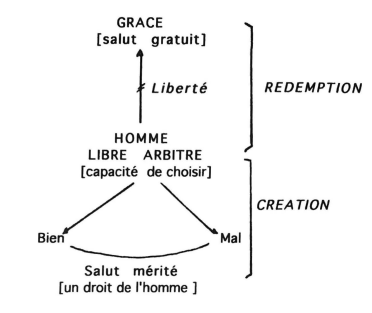
\includegraphics[width=\textwidth]{CoursTheo/Images/Augustin - Redemption.png}






A ce naturalisme, Augustin défend la thèse de la grâce. Dès 414, il entreprend de réfuter le livre de Pélage sur la «nature humaine». Il insiste sur deux aspects:

-	Une		nature	blessée.	Alors que Pélage insiste sur la bonté de la nature humaine, pensant ainsi rendre hommage et justice à son «créateur», Augustin lui reproche d'oublier que cette nature est blessée par le péché, ce qui la rend incapable de faire le bien sans l'intervention du «rédempteur».		Voici comment Augustin s'exprime :	«Mais, quand il (Pélage) croit servir la cause de Dieu en défendant la nature, notre auteur ne remarque pas qu'en déclarant cette nature saine, il évince la miséricorde du médecin...Or, nous ne devons pas louer le créateur de façon à nous trouver réduits à avouer que le sauveur est inutile.66»	Augustin n'ignore pas le libre arbitre, mais le pouvoir de choix ne devient efficace que s'il est d'abord libéré.

-	La nécessité du rédempteur. Alors que Pélage développe une théologie de la création, Augustin se fait le champion d'une théologie de la rédemption. Alors que Pélage met l'accent sur la liberté humaine, capable de choisir entre le bien et le mal, et donc capable de mériter son salut, Augustin estime que la liberté étant aliénée, elle ne devient capable de faire le bien que si d'abord elle a été restaurée dans son pouvoir
es Isabelle BOCHET, Saint Augustin et le désir de Dieu. Et. aug. , 1982, p. 320.
ee De natura et gratia 34, 39, in BA 24. Ppour une présentation d'ensemble, voir Paul Agaësse, L'anthropologie chrétienne selon saint Augustin. Image, liberté, péché et grâce. Centre Sèvres, Paris, 1980.
28	(
 
de,.1e faire. Or, étant donné le péché originel, seul Dieu peut redonner à l'homme ce qu ''· a perdu. If n'est donc pas légitime de s'attribuer à soi-même un quelconque ménte. Toute notre justification nous vient de Dieu et le salut est un don gratuit que nul n'a mérité par soi-même. "Tous ont péché" (Rm 5, 18), ce qui signifie que "personne n'est justifié si le Christ ne le justifie"67   Seule la foi dans le Christ rédempteur peut sauver l'homme, «la foi en Jésus Christ fait homme, la foi en son sang, la foi en sa croix, la foi en sa mort et en sa résurrection !88 » Il n'y a donc pas à hésiter sur la nécessité absolue de la grâce dans la condition de l'homme pécheur :
«Reconnaissons que la grâce est nécessaire; crions : Malheureux homme que je suis! qui me délivrera de ce corps qui me voue à la mort? Et que l'on réponde: la grâce de Dieu, par Jésus-Christ notre Seigneur.18 »

Quel est l'enjeu du débat ? Regardons d'abord la thèse	de Pélage. En gros, Pélage insiste fondamentalement sur la valeur de l'homme. A la création, Dieu a donné à l'homme la liberté et la raison, donc la possibilité d'exécuter volontairement le dessein de Dieu et donc de mériter par lui-même le salut. C'est une théologie de l'autonomie humaine, marquée au coin d'un certain naturalisme et d'un certain rationalisme. Pélage vantait les capactiés de la nature humaine. Cet optimisme au sujet des capacités de l'homme devait le conduire	à précher un volontarisme moral . L'homme pélagien est un être "sans reproche" :

« Ce n'est pas grand-chose, disait-il d'être un exemple pour les païens...Ce qui est beaucoup mieux, c'est d'être tel que les saints eux-memes soient édifiés.» (Cf. E.U.)

En face de ce naturalisme, qui menaçait de dévaloriser la grâce, Augustin réagit vivement en défendant la thèse de la grâce. Alors que Pélage insiste sur la bonté de la nature humaine, pensant ainsi rendre hommage et justice au "créateur" de cette nature, Augustin lui reproche d'oublier que cette nature a été blessée par le péché, ce qui la rend incapable de faire le bien et nécessite l'intervention du "rédempteur" et de la grâce. Voici comment Augustin s'exprime:

« Mais, quand il croit servir la cause de Dieu en défendant la nature, notre auteur ne remarque pas qu'en déclarant cette nature saine, il évince la miséricorde du médecin...Or, nous ne devons pas louer le créateur de façon à nous trouver réduits à avouer que le sauveur est inutile.» (De natura et gratia 34, 39, BA 24).

A l'arrière-plan de ce débat, on distingue à la fois deux  expériences différentes.

-	L'expérience d'Augustin est celle d'un converti qui s'est heurté à ses propres limites et pour qui sa conversion est l'expérience fondatrice de sa propre pensée. Le mouvement premier d'Augustin est toujours l'action de grâce pour ce que Dieu a fait de sa vie. Comme l'a bien noté G. Greshake : «Il est impossible, dans la prière, de se présenter à Dieu et de lui dire : Je dois mon salut à toi et à moi, à ce que tu as fait et à ce que j'ai fait. Dans la confessio, on peut dire seulement : ce que j'ai, je



67  De natura et gratia 41, 48.
88 lb. op. cit. 44, 51.
av Rom 8, 24-25, ib. op. cit. 53, 61.
29
 
te ledois.7»0	li dira encore : «Tu es miséricorde, je suis misère.» (Conf. X, 28, 39).	(

-  Pélage nous est  trop peu  connu pour savoir à quelle expérience pers n elle    e réfère. Ce qui est sûr, c'est qu'il représente un type de chnst,anisme qui fait appel en priorité non pas à la grâce, comme Augustin, mais aux capacités de l'homme.

\subsection{Nouvelle vague : les moines d' Adrumète et Julien d'Eclane}
 

Le jeu n'était donc pas calmé avec la condamnation de Pélage. Une nouvelle phase	Cela
allait se produire,	provoquée soit par certains disciples trop dociles d'Augustin, tels
les	moines du couvent africain d'Adrumète (Sousse, au Sud de Carthage), ou au
contraire par des disciples de Pélage, tel Julien d'Eclane.

- Les moines d' Adrumète répandirent, vers 425-426, l'idée que, puisque Dieu fait tout, la liberté n'est rien et n'a rien à faire. Prenant trop à la lettre certaines affirmations d'Augustin sur la grâce, ils en tiraient que la liberé est inexistante. Alors que les Pélagiens niaient la grâce au nom de la liberté, à l'inverse, ces moines défendaient «la grâce de Dieu jusqu'à nier le libre arbitre de l'homme». Augustin leur fit savoir que \sn{10 G. GRESHAKE, Geschenkte Freiheit. Einführung in die Gnadenlehre, Freiburg, 1977, p.
47.	Cité par Goulven MADEC, Pélage et Augustin. Le débat sur la liberté et la grâce.
Itinéraires augustiniens 13 (janvier 1995).}
\begin{quote}
    «confesser la grâce comme il l'avait fait, ce n'était pas nier le libre arbitre ni le mérite...» 
    \end{quote}
    
    Il écrit  à  Valentin, abbé du monastère :	
    \begin{quote}
        

 « Certains parmi vous exalteraient la grâce au point de nier le libre arbitre de
 l'homme, et, ce qui est plus grave, soutiendraient qu'au jour du jugement Dieu n'aura
 pas à rendre à chacun selon ses oeuvres...» (p. 53)	
«S'il n'y a pas de grâce divine, comment Dieu sauve-t-il le monde ? Et s'il n'y a	 pas de libre arbitre, comment juge-t-il le monde ?...Ne niez pas la grâce de Dieu, et
 ne défendez pas le libre arbitre jusqu'à le rendre indépendant de la grâce de Dieu,
comme	si nous pouvions sans elle concevoir	ou	accomplir quelque chose	selon	Dieu \sn{" De gratia et libero arbitrio. B.A. 24, p. 55. "Il en est qui défendent la grâce de Dieu
jusqu'à nier le libre arbitre de l'homme".	}     » (p.  SS)
    \end{quote}
 
Augustin invite à tenir ensemble les deux vérités : le libre arbitre	et la grâce. Il énumère alors une série d'affirmations tirées de l'Ecriture, les unes en
faveur de la grâce, les autres en faveur du libre arbitre. Si l'on ne peut pas	comprendre comment les deux s'articulent, il faut s'en tenir à l'Ecriture qui les
affirment simultanément \sn{B.A 24 p. 276 cf. aussi B.A. 73 B : page 480, la grâce et la liberté, et p. 477 ,
préscience divine et liberté humaine.}: 
\begin{quote}
    "Elle nous enseigne à la fois la réalité du libre arbitré · humain et la réalité de la grâce divine; grâce sans laquelle le libre arbitre ne peut ni se tourner vers Dieu ni progresser en Dieu.» (p. 59). 

\end{quote}

Y a-t- il une coordination possible des deux termes ? Augustin donne à la grâce une extension telle qu'elle englobe la liberté. La liberté est déjà grâce. La formule la plus parfaite pour exprimer le lien
entre les deux se trouve dans le "De correptione et gratia"  :	 
\begin{quote}
   «Aguntur  enim  ut	agant,  non  ut	ipsi nihil agantl» (11,  4)
«Ils sont en effet	agis pour agir, non pour ne rien faire» 
\end{quote}


-  Avec  Julien d'Eclane, le défenseur  de la liberté, le combat allait prendre une tournure plus dure. Julien invoquait à l'encontre d'Augustin un certain nombre de textes  sur la liberté - en fait sur le libre arbitre - que celui-ci avait écrits autrefois. Augustin sera obligé de rétablir ainsi l'équilibre, mais en mettant de plus en plus l'accent sur la grâce, si bien qu'on peut parfois se demander s'il réussit encore à reconnaître la place de la liberté. Il tire de !'Ecriture une série d'affirmations, les unes en faveur de la grâce, les autres en faveur du libre arbitre. Si l'on ne peut pas comprendre comment les deux s'articulent, répond Augustin, il faut s'en tenir à !'Ecriture qui les affirment simultanément : «Elle nous enseigne à la fois la réalité du libre arbitre humain et la réalité de la grlce divine; grlce sans laquelle le libre arbitre ne peut ni se tourner vers Dieu ni progresser en Dieu.»

L'affrontement entre Augustin et Pélage se joue sur l'idée que l'un et l'autre se font  de la liberté. Pour Augustin, le libre arbitre n'est pas la liberté, mais il est  la simple capacité de choisir,  de disposer librement de sa propre volonté.
« Notre volonté ne serait même plus volonté si elle n'était en notre pouvoir. Mais puisqu'elle est en notre pouvoir, elle est libre pour nous; car ce qui n'est pas libre pour nous, c'est ce qui n'est pas en notre pouvoir; et ce qui l'est ne peut pas ne pas être libre.73» Pélage n'a aucune peine à accepter cette définition. li la tirait même à lui pour démonter que Augustin n'était pas toujours Augustin, c'est-à-dire le champion intransigeant de la grâce. Seulement, alors que pour Pélage, le libre arbitre, confondu avec la liberté, est la capacité de l'homme à choisir entre le bien et le mal, pour Augustin, il se restreint  à la responsabilité de l'homme dans le mal : Il est la
«facuitas peccandi» (1, 16, 35).  Il est rare qu'il fasse appel au libre arbitre dans le choix du bien74   L'orientation vers le bien relève de· la liberté, la  «vraie»  liberté se manifestant dans la soumission à Dieu et n'existant que par la grâce. Or, la liberté qui s'est perdue en raison du péché, est incapable de se réenraciner dans le bien. Pour agir de nouveau selon Dieu, il faut une restauration de la liberté par la grâce. Pélage qui ne connaissait que le libre arbitre ne réalisait pas que, sans la grâce, donc sans la vraie liberté,  le libre arbitre était une serf-arbitre.

Si l'on voulait entrer plus avant dans ce débat, il faudrait évidemment évoquer le problème  de  la  prédestination, qui vient se greffer sur celui de la liberté. Puisque la liberté de l'homme n'est rien sans la grâce, n'est-elle pas une pure illusion, totalement régie de l'extérieur par une autre liberté, celle de Dieu, qui donne ou refuse sa grâce avant tout mérite de l'homme? C'est cette thèse que soutiendront les jansénistes, dont on reparlera. Augustin est moins radical. Mais ses propos sont souvent ambigus, sinon choquants 75   La polémique l'a parfois entraîné dans certains

73 Sur le libre arbitre 111, 3, 8. Cf. G. Madec, Itinéraires augustiniens 13 (janvier 1995.
H Cf. Enchiridion XXVIII, 106. «Car si le péché dépendait du libre arbitre seul, cependant, pour conserver la justice, lelibre arbitre ne suffisait pas si la la participation du bien immuable ne lui assurait le secours divine.»
H Cf. Enchiridion XXIII, 93. BA 91 p. 269 : «Bénigne entre toutes,à ne pas douter, sera la peine de ceux qui au péché qu'ils tenaient de leur origine se gardèrent d'en ajouter aucun.» Cette thèse a été exacerbée par les jansénistes et les calvinistes, qui ont introduit l'idée d'une prédestination négative, Dieu décidant arbitrairement, d'avance et de façon absolue, de
la destinée éternelle de chaque être.
31
 
dé pages, par exemple lorsqu'il écrit, à propos des vertus des païens, qu'elles ne sont	(
qu enflure et orgueil et, on doit, à ce titre, les regarder, non comme des vertus, mais
comme des vices»76 ; ou à propos des enfants non baptisés, lié au problème de la Prédestination, qui sont à jamais exclus de la béatitude, même si leur peine est
atténuée. La prédestination est un mystère qui renvoie à l'insondable volonté de Dieu. Si Augustin n'a pas toujours la formule équilibrée de ce mystère, puisque la volonté de Dieu est, d'une part «que tous les hommes soient sauvés», mais que d'autre part
«beaucoup plus grand est le nombre de ceux qui ne le sont pas», il refuse cependant toujours les excès auxquels certaines de ses formules se prêtaient77  L'exemple de la prédestination est le plus significatif. Augustin s'interdit de l'enseigner comme s'il s'agissait d'un fatalisme, réduisant à néant la liberté78 

S. Plaidoyer  en faveur de la grâce71

Augustin ne prétend pas avoir une théologie personnelle. Son unique livre de théologie est !'Ecriture. C'est pourquoi, il faut voir sur quels textes il appuie l'absolu de la grâce dont il se fait le champion face aux Pélagiens . Je voudrais citer quelques textes clefs qui lui servent à appuyer ses affirmations sur la grâce«>

a.	"Qu'as-tu que tu n'aies reçu... Et si tu l'as reçu, pourquoi t'en faire gloire comme si tu ne l'avais pas reçu ?" (1 Co 4, 7). Et voici le commentaire :

« C'est principalement ce témoignage de /'Apôtre qui m'a convaincu moi-même, quand j'étais dans une erreur semblable à celle de nos frères - il s'agit des moines de Provence - et je m'imaginais que la foi, par laquelle nous croyons en Dieu n'est pas un don de Dieu, mais que nous l'avons de nous-mêmes, et que nous obtenons ainsi par elle les dons divins qui nous permettent de 'vivre en ce monde avec modération' (Tit 2, 12). Je ne voyais pas que la foi est précédée en nous par la grâce de Dieu, pour que par elle nous soit ensuite donné ce que nous demandons utilement...»(De praedestinatione sanctorum 3, 7, B.A. 24 p. 479)
«La foi elle-même figure parmi les dons divins qui nous sont dispensés en ce même Esprit. Ces deux choses : croire et agir, sont nôtres en raison de notre libre arbitre, et cependant l'une et l'autre sont données par /'Esprit de foi et de charité. Car ce n'est pas la charité seulement, mais, comme il est écrit, "la charité avec la foi qui descend de Dieu le Père et du Seigneur Jésus-Christ" (Eph 6, 23).(ib. 3, 7, p. 481-483)





18 Cf. Cité de Dieu XIX, 25, . BA 37, p. 165-167, et p. 761, avec d'autres références p. 957. J. WANG TCH'ANG-TCHE, Saint Augustin et les vertus des païens. Beauchesne, 1938.
11 Enchiridion XXIV, 97 s.
78 Voir par exemple : De dono perseverantiae, 22, 57, BA 24, p. 741, et autres référence page 859. Augustin précise «la manière dont il convient d'enseigner la prédestination», insisitant sur le fait qu'on doit éviter de la présenter «de façon à la rendre odieuse».
79 Voir le dossier scripturaire dans Sesboüé, op. cit. p. 167.
8°Ces textes ont été sélectionnés par Jacques Pintard, Le docteur de la grâce, in Augustin, le
message de la foi, DDB, 1987, pp. 119 sv.:


32
(
 
b.	"Personne ne peut venir à moi si le Père qui m'a envoyé ne l'attire" (Jo 6, 44) "Magnifique éloge de la grâce! Nul ne vient s'il n'est tiré..." (26, 2, BA. 72, p. 487). Aussi est-ce juste de glorifier Dieu pou les mérites : "Lo!"5que tu couronn s leurs mérite tu couronnes tes propres dons. (Lettre 194, à Sixte, 19). Augustm illustre un u plus loin sa pensée par une comparaison cet attrait qu'exerce le Père
pour l'attacher au Christ :
«Donne-moi quelqu'un qui aime, et il sentira la vérité de ce que dis. Donne-moi un homme tourmenté par le désir, donne-moi un homme en marche dans ce désert et qui a soif, qui soupire après la source de l'éternelle patrie, donne-moi un tel homme, il saura ce que je veux dire.» (lb. 26, 4, pp. 491-493).
«Tu montres  un rameau vert à une brebis, tu l'attires. On présente des noix à
un enfant, il est attiré...Si donc ce qui est révélé des délices et des voluptés terrestres à ceux qui les aime les attire, ...comment le Christ révélé par le Père n'attirerait-il pas ? » (ib. 26, s, p. 497).
c.	"Dieu résiste aux orgueilleux et donne sa grâce aux humbles" (Proverbes 3, 34, et cité en I P 5, 5 et Jac 4, 6). Augustin cite SS fois cette sentence dans son oeuvre, selon la comptabilité de La Bonnardière. Elle indique qu'il n'y a pas d'autre voie vers Dieu que l'humilité du Verbe.

Augustin, on l'a vu, fut profondément marqué par cette découverte du Christus humilis. Le grand obstacle à la rencontre de Dieu est l'orgueil: "Dieu s'est fait humble, et l'homme est orgueilleux" (Sermon 142, 6)

d.	"Donne ce que tu commandes et commande ce que tu veux" Da quod jubes et jube quod vis ! (Conf. X, 29, 40; 31, 45; 37, 60). Augustin lui-même rappelle combien cette sentence avait irrité Pélage. Il écrit dans le De dono perseverantiae :
\begin{quote}
    « Parmi mes ouvrages, en est-il un qui ait été plus répandu et plus goûté que mes Confessions ? Or, dans cet ouvrage, publié lui ausi avant que n'eût paru l'hérésie pélagienne, je dis, et plusieurs fois à notre Dieu :"Donnez ce que vous commandez et commandez ce que vous voudrez." Ce sont ces paroles de moi que Pélage, à Rome, entendit un jour citer par un de mes frères et collègues dans l'épiscopat; il ne put les supporter, et dans l'émotion vive qu'il mit à les contredire, peu s'en fallut qu'il se prit de querelle avec celui qui les avait rappelées. Mais qu'est-ce que Dieu nous commande d'abord et par dessus tout, sinon de croire en lui ? Donc, c'est lui qui nous donne de croire..." (B.A. 24, 20, 53)
\end{quote}


\begin{quote}
    L'espérance ne déçoit point, parce que l'amour de Dieu a été répandu dans nos co ur par le Saint-Esprit qui nous fut donné" (Rom 5, 5). 
\end{quote}
Un verset qui est cité pas moins de 200 fois. Augustin précise:
\begin{quote}
    « · Quand nous disons que Dieu aide à accomplir toute justice et opère en nous le vou o r et le faire (cf. Ph 2, 13) ... ce n'est pas parce qu'il fait ressentir en nos sens xt ieurs les préceptes  de la justice, mais parce qu'il donne l'accroissement mt neur   I Co 3, 7), en répandant la charité dans nos coeurs par /'Esprit-Saint
qw nous a ete donne» (L'esprit et la lettre 25, 42)

\end{quote}

 
 
Loin de contredire le libre arbitre, la présence de !'Esprit le dégage au contraire	( pour le rendre libre : "Partout où est !'Esprit du Seigneur, là est la liberté (2 Co 3,
17, là, le coeur humain est dilaté, ce qui fait dire à Augustin : « Cet Esprit de Dieu dont
la présence nous justifie, nos inspire la haine du péché et nous donne la liberté spirituelle» (ib. 16, 28).

\subsection{Nouveaux	rebondissements sur liberté et	grâce}
 

La thèse de la prédestination rebondit plusieurs fois au cours de l'histoire. Qu'il suffise de donner quelques points de repères. Trois moments, de plus ou moins d'ampleurs, on marqué ce débat.

a)	La question rebondit une première fois au IXe siècle, avec les thèses d'un moine, Gottschalk\sn{81 Cf. Kurt FLASCH, Introduction à la philosophie médiévale, Cerf, Ed. universitaires de Fribourg, 1992, p. 29 s., en particulier p. 33 s. sur Godescalc et la prédestination divine.} , fils d'un prince saxon, qui vivait au monastère d'Orbais (diocèse de Soissons). D'un esprit étroit, il enseignait que Dieu prédestine aussi bien les damnés à l'enfer que les élus au ciel. L'idée même de prédestination absolue entraîne aussitôt chez Gottschalk la négation de la liberté. De plus, introduisant I' idée d'une prédestination négative, il transforme Dieu en monstre, puisqu'il devient l'auteur du pire mal qui puisse arriver à l'homme. Inutile d'ajouter que, dans ces conditions, la rédemption laisse totalement hors de son champ ceux qui sont d'avance exclus du salut.

Cette théorie monstrueuse, qui se prétend l'expression de la pensée d'Augustin, sera condamnée : le concile de Valence (855) réaffirmera l'universalité du salut et la rédemption de tous, en même temps qu'il rcconna1t .; tout homme la liberté et le pouvoir de se sauver. Durant le Moyen Age, c'est cet augustinisme tempéré qui va s'imposer. Sans rien enlever à l'absolu de la grâce, les scolastiques partiront de l'idée de l'universalité du salut, une doctrine qui était passée quelque peu sous silence, et le reste, c'est-à-dire grâce et liberté, y est subordonné. Pour sauver les hommes, Dieu n'est pas tenu par les sacrements, dira saint Thomas. Il dispose de bien d'autres moyens.

b)	Avec  la  Réforme,  la  question  deviendra  beaucoup  plus  aiguë. Luther et Calvin se réclament tous les deux d'Augustin. De tous les auteurs anciens, Augustin est à leurs yeux le meilleur interprète de !'Ecriture. «Augustinus  meus totus est», déclare Luther dans sa polémique avec Erasme : «De ton côté sont les théologiens modernes et tant d'universités, de conciles, d'évêques, de papes! ...De mon côté, au contraire, seulement Wyclif et Laurent Valla, mais aussi Augustin, que tu passes sous silence, m'appartient tout entier.» De même, Calvin se place sous l'autorité  d'Augustin,  qu'il  cite  341  fois  dans  la  seule  Institution  chrétienne.
«Augustinus totus noster est», écrit-il en écho à Luther : «Quant à saint Augustin, il s'accorde si bien en tout et partout avec nous, il est tellement nôtre (adeo totus noster est) que s'il me fallait écrire une confession sur cette matière, il me suffirait de la composer des témoignages extraits de ses livres... Je ne dis rien qu'il n'ait dit devant moi mot à mot.» Si l'on considère ce qui a séduits les Réformateurs, c'est, on s'en doute, la doctrine augustinienne de la grâce et de la justification. Chez Calvin, c'est toujours dans le contexte de sa défense de la prédestination qu'il cite Augustin, sans
s'apercevoir que l'idée d'une double predestination, le salut pour les uns et la J>erdation Pour les autres, dont il se fait le défenseur, est totalement étrangère à Augustin\sn{82 Cf. Augustinus Magister. Etudes augustiniennes, 1954. Il, 1029 s. pour Luther et saint Augustiin (Léon Cristiani), et 11, 1839 s. pour Calvin et saint Augustin (Jean Cadier).
63 Léon CRISTIANI, Luther et saint Augustin, dans Augustinus Magister Il, 1954, p. 1037 -1038.
84 Cf. Henri de LUBAC, Augustinisme et théologie moderne. Aubier, 1965, p. 15 s.}

Quand en effet on y regarde de plus près, on s'aperçoit que, au-delà de l'appel explicite à son autorité, Augustin ne sert chez Luther et Calvin qu'à cautionner des thèses qui sont les leurs plus que les siennes. Cet a priori de lecture est évident chez Luther. Alors même qu'il se croit dans la ligne d'Augustin, il oublie des pans entiers de sa pensée. En particulier, sa thèse sur la justification ne saurait être tirée d'Augustin sans autre forme de procès. Augustin ne dissocie jamais foi et charité. Alors que Luther soutient que la foi seule justifie, Augustin dit que c'est la charité dans son obéissance à la loi. Luther n'a d'ailleurs pas été sans lui-même relever cet écart. Mais au lieu de rectifier sa propre position, il accuse Augustin d'inconséquence ou d'infidélité à lui-même. Melanchton, avec l'accord de Luther, avouera explicitement à Brenz : Augustin, qui avait d'abord nié que l'homme puisse être justifié par lui­ même devant Dieu, «imagine ensuite que nous sommes réputés justes en raison de l'accomplissement de la loi que le Saint-Esprit opère en nous... Augustin n'est pas en accord complet avec la doctrine de saint Paul, bien qu'il en approche davantage que les Scolastiques... » Il ajoute que, pour le public, il faut continuer à invoquer l'appui d'Augustin, «bien qu'il n'explique pas assez la justice par la foi»83 

c)	Le	jansemsme	représente	le	troisième	rebondissement.	Sa préhistoire commence avec Michel Baius (1513-1589), chancelier de l'université à Louvain, qui avait fait d'Augustin son cheval de bataille contre les protestants. Il avait lu, nous dit-on, neuf fois tout saint Augustin et soixante-dix fois les écrits sur la grâce f Ce qui ne l'a pas empêché de se fourvoyer sérieusement. Le point névralgique de sa position tourne autour du rapport entre nature et grâce. Dans l'état initial d'Adam, la «nature» de l'homme était dotée d'une puissance autonome en face de Dieu, c'est-à­ dire d'une liberté capable par elle-même de faire son salut, si bien que si l'homme était fidèle à sa nature, il pouvait en droit prétendre à la récompense. «Chez l'homme d'avant la chute, la vie éternelle... n'aurait pas été un don de la grâce, mais un salaire.» C'est la thèse de Pélage : «Dieu me fait homme, mais c'est moi qui me rend juste», sauf que Baius parle de la condition de l'homme	d'avant la chute, tandis que . Pélage parle de sa condition actuelle .

On a dit de Baius qu'il était un «Pélage  du  paradis  terrestre». Depuis la chute, en effet, la grâce est devenue indispensable à l'homme, comme un ajout extérieur à une nature blessée et déficiente, alors qu'elle ne l'était pas avant. En se voulant fidèle à Augustin, Baius en fait le trahit, car pour Augustin,aussi bien dans l'état primitif que dans l'état actuel, sans la grâce, l'homme est incapable de parvenir au salut. Adam, pas plus que l'homme déchu, ne peut s'attribuer à lui-même un quelconque mérite.  	Au fond, Baius n'a sauvé Augustin qu'au prix d'une double déformation, à la fois du concept de nature et du concept de la grâce. Au regard de la pensée d'Augustin, l'extrinsécisme de Baius est une aberration. Mais la question se pose aussitôt : Baius, qui a été condamné, n'aurait-il pas entraîné dans sa chute Augustin lui-même? C'est ce que prétendaient certains jésuites.


 
C'est pour réfuter cette prétention que Jansénius (1585-1638), fu ur évê ue d'Ypres, rédige un ouvrage de synthèse sur la pensée d'Augustin : I' Augustmus qui ne sera publié qu'après sa mort, en 1640, et dont les jansénistes eront leur Bible. De Jansénius aussi, on nous dit qu'il avait lu «dix fois saint Augustm, et plus d? tren e fois les ouvrages de la grâce contre les Pélagiens», ce qui ne l'empêche pasd aboutir, en fin de compte, à une «consciencieuse méprise». En réalité, il ne fait que prolo,nger Baius, mais en l'inversant. Alors que Baius part d'une nature qu1, au moms dans I état d'Adam, peut prétendre au salut, la grâce devenant inutile, Jansénius part de l'absolu de la grâce, expression de la puissance arbitraire de Dieu, qui la donne ou la refuse sans tenir compte de l'homme, pour refuser ensuite à la nature humaine, d nc à la liberté, toute consistance propre. «Si l'un et l'autre tendent également à dissoudre l'union entre Dieu et l'homme en quoi consiste essentiellement le Mystère du Christ, écrit le P. de Lubac, n'est-ce pas que l'un dresse l'homme en face de Dieu dans la réclamation de ses droits, tandis que l'autre l'anéantit ?fJS »
La thèse de Jansénius sera à l'origine de tous les débats modernes autour de la grâce, dont Port-Royal,  avec l'abbé de Saint-Cyran à sa tête, sera le foyer en France. Délaissant les spéculations de Baius sur l'état primitif de l'homme, tout comme celles de Jansénius sur la «pure nature», Saint-Cyran s'intéresse à l'homme concret, pour le placer d'emblée devant le mystère redoutable de la grâce, une grâce rare, qui n'est donnée qu'à un petit nombre d'élus. «Comme le soleil fait des jours sacrés et des jours profanes, des jours de fête et des jours civils, des jours d'été et des jours d'hiver, ainsi Dieu a fait certains hommes pour être sauvés et saints, et d'autres profanes pour être damnés... ». «li ne tombe pas une goûte de grâce pour les païens !» Saint-Cyran, sans lequel le jansénisme n'aurait sans été qu'une «hérésie de professeurs», lui assurera le succès. Mais c'est bien à tort qu'il invoque saint Augustin. A aucun moment, Augustin n'a pensé que le destin de l'homme pouvait être scellé de l'extérieur par Dieu, sans que la responsabilité de l'homme y soit engagée. Alors que les débats sur la grâce et la prédestination, tels qu'ils se sont développés dans le jansénisme, se placent au point de vue de l'éternité, où tout semble joué d'avance, Augustin considère l'homme dans son devenir temporel, où l'alternative entre la lumière et les ténèbres reste toujours ouverte86 

\section{Conclusion}
\begin{Synthesis}
 Augustin maintiendra contre vents et marées le primat de l'action de Dieu. Il n'a pas réussi à concilier par des concepts l'action de Dieu et l'agir de l'homme. Le champion de la liberté contre les manichéens s'est battu avec la même i tran igeance en s faisant le champion de la grâce contre les Pélagiens. Augustin s'en tient a la parole de l'Ecriture, faisant siennes ce texte de l'Apôtre: .
\begin{quote}
    «  Qui es- tu pour discuter avec Dieu ? (Rm 9, 20)  Impénétrables  sont ses Jugements et incompréhensibles ses voies (Rm 11, 33) Et il ajoute : "Ne cherche pas a atteindre ce qw est trop haut pour toi, ni à scruter ce qui te dépasse"» (Ecc 3, 22) (De Dono perseverantiae XII, 30, B. A. 24 p. 669)
\end{quote}
\end{Synthesis}




Au cours des siècles, cette doctrine de la grâce fut tirée vers une doctrine intolerable, celle de la prédestination, et en particulier de la prédestination négative, notamment chez les Jansenistes et les calvinistes. Dieu est alors un Dieu arbitraire,
pervers, qui décide d'avance, de façon absolue, qui va au ciel et qui va en enfer, indépendamment des mérites :
\begin{quote}
    « Par décret de Dieu, et pour la manifestation de sa gloire, tels hommes sont prédestinés à la vie éternelle, tels autres voués à la mort éternelle!» (Confession de Westminster, 1647).
\end{quote}


Une telle doctrine n'est pas augustinienne, même si certaines formules peuvent être tirées en ce sens. Mais il faut bien constater que ce sont ces excès modernes qui furent à l'origine d'une certaine forme d'athéisme, l'athéisme humaniste, qui oppose Dieu et l'homme, la grâce et la liberté, et qui rejette Dieu au nom de l'homme et de la liberté.
\begin{quote}
    "M'en coûtât-il d'être expédié en Enfer, disait Milton, jamais un tel Dieu ne m'imposera le respect!" (Cf. Max WEBER, L'éthique protestante et l'esprit du capitalisme, Pion, p. 117.)
\end{quote}"M'en coûtât-il d'être expédié en Enfer, disait Milton, jamais un tel Dieu ne m'imposera le respect!" (Cf. Max WEBER, L'éthique protestante et l'esprit du capitalisme, Pion, p. 117.)

Augustin était trop conscient de la liberté de l'homme pour croire qu'elle pouvait être mise en échec par la grâce. Celle-ce n'est pas contre la liberté, ni au-dessus de la liberté, mais avec la liberté qu'elle rachète et rend efficace dans l'ordre du salut. L'acte le plus libre est celui par lequel l'homme accepte de reconnaître que tout lui est donné, y compris sa liberté.
 
























37

%

% \chapter{Lire les classiques Chinois}

 

\textbf{Comment lire les classiques chinois ? (French Edition)}

\textbf{Vermander, Benoît}

\section{Prologue}


\subsection{Période axiale}
  \mn{ p. 5 · E. 59  } \begin{quote}
Lorsque la notion même de « période axiale » est acceptée au moins comme
hypothèse de travail ( elle est parfois rejetée dès l'abord ) , les
percées qu'on lui associe sont généralement les suivantes : ( a ) les
penseurs de la période auraient contribué à « problématiser le monde »
plutôt qu'à le recevoir tel quel , ce par le fait d'articuler la réalité
sociale autant que naturelle autour de questions portant sur son «
pourquoi » et son « comment » ; ( b ) c'est ainsi qu'aurait émergé la «
conscience critique » , l'examen des opinions reçues , la remise en
cause d'au moins certaines des structures sociales ; ( c ) ce
questionnement
aurait nourri un souci éthique ( à moins que ce dernier ait contribué à
l'émergence de la conscience critique ) , souci qui fut accompagné
souvent de la formation d'une vision utopique -- la cité idéale de
Platon , la pleine libération des individus dans le bouddhisme , le rêve
d'un ordre social gouverné par les rites , l'éducation morale , chez
Confucius , l'annonce de la venue du Royaume de Dieu chez les prophètes
d'Israël ; ( d ) le surgissement critico - éthique aurait été porté par
des personnalités incarnant les « sauts » entrepris , personnalités dont
le nom est transmis aux générations qui leur succèdent ; ( e ) ces
personnalités sont souvent représentées ( et semblent s'être considérées
elles - mêmes ) comme des « Renonçants » , des individus dont les choix
de vie mettent en question l'ordre dominant : dans la République , le
philosophe de la cité idéale de Platon renonce aux possessions privées
et à la vie de famille pour gouverner la Cité avec justice

\end{quote}  

\subsection{Divination, mathématique et concepts}
\mn{- p. 17 · E. 258  } \begin{quote}  

Élaborer des ramifications entre les principaux viscères du corps humain
et les états climatiques ( le chaud , le froid , le sec , l'humide ) ,
les émotions , les notes de musique , les couleurs , tout cela transcrit
dans une arithmétique de
base cinq » , n'est pas simple opération de l'esprit mais permet bien
d'observer pragmatiquement un ensemble de correspondances . En même temps, ces analogies deviennent moralement signifiantes. C’est ainsi que s’opère une évolution du divinatoire au combinatoire et à l’éthico-politique.   
A la fois matrice de ce processus et l'accompagnant tout au long de sa
formation textuelle , le \textit{Classique des mutations ( Yijing )} construit un
métalangage de l'univers à partir d'une réflexion mathématisée sur les
processus de divination.
il s'essaie à décrire la façon dont les phénomènes se suivent et
s'agencent de façon nécessaire . C'est , à l'extrême , une mathématique
de tous les phénomènes possibles , fondée sur l'idée que tout n'existe
que dans l'échange , le passage , la fluidité : la gradation est un
autre nom du contraste , et la logique des transformations ( des
changements par quoi une forme entre en contraste avec celles qui la
précèdent et la suivent ) , non pas celle des oppositions , régit
l'univers et la pensée .

\end{quote} \mn{ p. 18 · E. 268 } \begin{quote}

Au ciel se composent les images {[} xiang {象} {]} , sur la terre se
composent les formes {[} xing 形 {]} , et les transformations se font
visibles {[} Yijing , Xici 繫辭 I . 1 {]} 28 .

\end{quote} 

\paragraph{le rite comme éducation} chez Confucius
\mn{p. 20 · E. 304  } \begin{quote}

Le vecteur de l'éducation ainsi dispensée , ce sera le rite
: l'éducation de l'intérieur par l'extérieur . À noter pourtant que « le
rite » ( chinois ) et « la loi » ( en contexte grec ou hébreu ) ne se
trouvent pas dans un strict régime d'opposition : ils régulent tous deux
les conduites extérieures jusqu'au moment où les prescriptions se
retrouvent être inscrites « au fond des cœurs » .

\end{quote} \mn{ p. 24 · E. 367 } \begin{quote}

La détermination d'un corpus de classiques fonde une culture dans sa
spécificité tout en lui donnant d'affirmer son l'universalité latente .
Hans - Georg Gadamer fait de l'extensibilité ,  en principe illimitée, de la durée pendant laquelle une œuvre communique son sens le trait qui désigne un « classique »
\end{quote} 
 
\section{Chapitre I : Qu'est-ce qu'un classique chinois ?}

\mn{ p. 37 · E. 786 } \begin{quote}

Du reste , dès les premiers rencontres entre lettrés chinois et
missionnaires occidentaux , les uns et les autres comprennent que le
continent qui leur fait face est fondé sur une armature de classiques
dont la maîtrise est essentielle pour la réussite culturelle ,
religieuse et sociale , et ils feront de la connaissance réciproque de
ces textes la clé d'une rencontre possible , d'une entrée dans la pensée
de l'Autre , que ce soit pour l'apprécier ou l'utiliser , pour
convaincre ou dominer l'interlocuteur .

\end{quote} \mn{p. 38 · E. 805  } \begin{quote}
On trouve cette acception chez Yang Xiong 揚雄 (53 AEC-18) :

 
 \begin{quote}
     : « Un texte qui ne se mesure pas aux Classiques n’est pas un texte. Une parole qui ne se mesure pas aux Classiques n’est pas une parole. Ce sont des excroissances qui prolifèrent  
 \end{quote}
La formule, très concise, pourrait aussi être comprise comme signifiant : « Un texte qui n’est pas (qui ne tend pas au) Classique n’est pas un texte. » Ou même plutôt : \textit{« Un texte non référé à une norme n’en est pas un. »} Le registre sémantique du passage 11 rappelle celui qui entoure le terme déjà évoqué κανών : l’instrument qui norme (la règle du charpentier en grec) donne naissance à un ensemble textuel établi par rapport à lui – ensemble qui, de normé, devient alors normatif.
 
\end{quote} \mn{p. 44 · E. 926  } \begin{quote}

Pouvoir {[} di {]} d'en haut {[} shang {]} » surplombe le monde
surnaturel ( ne parlons pas d'un « panthéon » ,car on n’y trouve pas l’individuation des divinités qu’on attache d’ordinaire à ce terme).

 

\end{quote} \mn{ p. 45 · E. 951 } \begin{quote}

L'autre chapitre des Documents sur lequel nous nous arrêterons
brièvement est celui du Hongfan 洪 範 , expression que l'on peut
traduire par « Grand plan » ou , sans doute plus justement , par «
Modèle universel » . Il présente l'ensemble des phénomènes ( éléments ,
conduites , matières politiques , calendrier , sources de bonheur et
malheur ) sur des combinaisons fondées sur les chiffres Cinq et Neuf .
Sa composition apparaît si rigoureuse que certains formalistes russes
ont spéculé sur son nombre de caractères et leur inscription à
l'intérieur d'un carré magique 30

\end{quote} 

\paragraph{les annales historiques} attribuées à Confucius : essayer de dicerner les signes des temps. 
\mn{ p. 56 · E. 1164 } \begin{quote}
les lecteurs de ces Annales vont s’employer à faire émerger des sens, à trouver l’expression du mandat du Ciel dans cette succession d’événements qu’ils vont lire comme une sorte de rébus. C’est dire que ce sont les commentaires suscités par l’œuvre qui en font tout l’intérêt.
[..]
Au travers de la sèche prose des Printemps et
  Automnes , le Gongyang s'emploie à trouver « le sens profond de paroles
subtiles"
\end{quote}


Importance du processus de mémoire.

 \mn{p. 59 · E. 1228  } \begin{quote}

Au travers de cet hommage rendu par les historiographes du Zuozhuan à
leurs prédécesseurs se donne à lire leur conviction : l'enregistrement
et la qualification fidèles des événements sont questions de vie ou de
mort . Cela parce que l'enchaînement des actions , des prédictions que
l'on en tire , de la vérification ou non de ces prédictions constitue la
trame de l'ordre du monde , et qu'en altérer le récit , c'est forcément
en distordre la marche .

\end{quote}

\paragraph{Anectdote : matériau de la connaissance historique} car elle offre un aperçu soudain sur une réalité plus profonde et étendue, comme la citation. \mn{ p. 59 · E. 1233 } \begin{quote}
Du fait de la nature même de ces deux extraits, on aura noté la place que joue, dans le Zuochuan, le genre littéraire très particulier de l’anecdote.
 
Elle est révélatrice d'une tendance plus générale : l'anecdote , dans
l'historiographie chinoise , deviendra le matériau même de la connaissance historique.
 

\end{quote} 
\subsection{le sacrifice comme lieu de l'unité}
Une partie des textes classiques visent à expliquer la tenue en cas de non respect du sacrifice. Cette importance peut étonner.
\mn{p. 65 · E. 1345  } \begin{quote}

C'est en distinguant qu'on peut droitement unir .
Le

mode de découpe de l'animal sacrifié puis la façon dont on répartit les
parties découpées constituent des opérations destinées à symboliser et
réaliser la cohésion du groupe , dans un modèle qui associe exigence
d'unanimité et affirmation de principes hiérarchiques stricts . 

\end{quote} \mn{ p. 66 · E. 1353 } \begin{quote}
Le sacrifice
était donc image inversée de l'ordre social effectif . La supériorité
sociale était étroitement associée à la capacité de donner .

\end{quote} \mn{  p. 66 · E. 1356 } \begin{quote}

Les anomalies rituelles relevées par les textes fonctionnent alors comme
informations historiques d'importance particulière . La crise rituelle
est toujours symptôme de crise politique .

\end{quote} \mn{ p. 66 · E. 1357 } \begin{quote}

le Liji traduit une anxiété face à tous les dysfonctionnements possibles
de l'activité rituelle , et , de ce fait , du travail social .

\end{quote} \mn{p. 67 · E. 1368  } \begin{quote}

Le rituel est donc affecté par une tension entre son but avoué -- édifier ,
maintenir un ordre -- et le fait qu'il soit par essence une entreprise
risquée , soumise à divers aléas .

\end{quote} 
\subsection{La grande Etude - Daxue}
\mn{p. 67 · E. 1384  } \begin{quote}

Tentons après tant d'autres une traduction de cette célébrissime entrée
en matière -- sachant qu'aucun lecteur ni commentateur n'arrive à faire
vraiment abstraction de la lecture qu'en ont effectué Zhu Xi et ses
continuateurs . 
\begin{quote}
    La voie de la Grande Étude 96 , c'est d'éclairer {[} le
principe de {]} vertu qui {[} lui - même {]} éclaire {[} toute chose {]}
, c'est d'aimer {[} ou bien de « renouveler » , selon les versions {]}
le peuple , et c'est de ne s'arrêter qu'une fois la plus haute
perfection atteinte . Sachant le terme , on prend sa détermination . Une
fois déterminé , on peut s'apaiser {[} jing 靜 97 {]} . Une fois apaisé
, on peut s'ancrer dans la paix . Quand on est ancré dans la paix , on
peut discerner . Ayant discerné , on peut atteindre le but . Les plantes
ont racine et branches , les affaires un commencement et une fin . Celui
qui sait la succession des affaires , il est tout proche de la voie .
大學之道,在明明德,在親[新]民,在止於至善。知止而后有定,定而后能靜,靜而后能安,安而后能慮,慮而后能得。物有本末,事有終始,知所先後,則近道矣。


\end{quote}


\end{quote} \mn{ p. 69 · E. 1411 } \begin{quote}

La partie gauche du caractère , sa clé sémantique , c'est le jade ( yu 玉 )
. Associée à l'autre partie du caractère , cette clé donne à l'ensemble
un tour plus abstrait : elle parle d'une structure sous - jacente aux
phénomènes qui prennent corps . Les Chinois ont trouvé dans les nervures
du jade la plus marquante des expressions des forces vitales qui , à
l'interne , structurent l'organisme.

\end{quote} 
\paragraph{L'invariable milieu, à l'autre extremité des quatre livres}
\mn{ p. 69 · E. 1420 } \begin{quote}
Comme pour la Grande Étude, voyons à traduire le premier paragraphe du texte :
\begin{quote}
La loi du Ciel 101, c’est ce qu’on appelle « la nature » 102. Se conformer à la nature, c’est ce qu’on appelle « la voie ».
\ldots

   Aussi , l'homme de bien se tient sur ses gardes même quand il ne
distingue rien {[} d'inquiétant {]} , il craint et tremble même quand
rien ne frappe son oreille . 
 
\ldots

Aussi , l'homme de bien reste sur ses gardes {[} même {]} dans la
solitude 104 . N'émettre {[} fa 發 {]} ni joie ni colère ni tristesse ni
allégresse , c'est ce qu'on peut appeler l'équilibre {[} le milieu {]} .

\end{quote} 
\end{quote}

Relecture

\paragraph{Xunzi : la discrimination fait l’homme
 }
\mn{ p. 72 · E. 1482 } \begin{quote}

On a argué , à mon sens fort justement , que le caractère fen 分 (
séparer , diviser ) constitue une clé -- sinon la notion clé -- du Xunzi
112 . Le fait que l'on compte 113 occurrences du caractère dans
l'ouvrage est un premier signe de son importance .

\end{quote} \mn{ p. 73 · E. 1493 } \begin{quote}

le principe de base sur lequel Xunzi fonde sa théorie politique est que
les désirs ( par essence subjectifs ) sont par nature illimités , tandis
que les biens sont objectivement limités ( yu duo er wu gua 欲 多 而 物
寡 113 ) . Savoir comment répartir et partager , c'est bien là l'essence
de l'art politique 114 . Xunzi pose ici l'accent sur la notion de gong
公 : gong ( habituellement traduit par « chose publique ») consiste à diviser quelque chose avec impartialité, sans afficher égoïsme ou partialité (si 私).
 

\end{quote} \mn{ p. 74 · E. 1510 } \begin{quote}
Le rituel, manifestation privilégiée des distinctions ainsi effectuées, devient alors le conduit par quoi ce qui était au départ
de l'ordre de la nature ( xing 性 ) se transforme en artifice ( wei 偽 )
, ce dernier terme revêtant un sens éminemment positif
 
\end{quote} 
Sens positif de l'artifice chez xunxi.
\begin{Def}[artifice]

\end{Def}
\mn{ p. 74 · E. 1522 } \begin{quote}

Xunzi trace une distinction entre les niveaux atteints respectivement
par le Lettré ( shi 士 ) , l'homme de bien ( junzi 君子 ) et le sage (
shengren 聖人 ) , ce dernier seul capable de fusionner en un tout la
perfection des dispositions à l'interne et celle atteinte par les
observances extérieures .



\end{quote}


Cf vie digne et vie parfaite

\mn{p. 75 · E. 1527  } \begin{quote}

Les châtiments contribuent à assurer l'équilibre entre hiérarchie et
impartialité .

\end{quote} \mn{ p. 76 · E. 1550 } \begin{quote}

Xunzi voyait bien la nature humaine ( xing 性 ) comme mauvaise ( e 惡 )
, il discernait dans l'artifice rituel couplé à la droite éducation la
route par laquelle s'ouvrait la possibilité de dépasser l'inné , jusqu'à
rendre chacun capable de devenir -- en théorie -- semblable aux sages souverains du temps passé. Route trop dangereuse pour le Hanfeizi, quand les États font face à des risques imminents (la principauté dont Han Fei est un dignitaire éminent va disparaître trois ans après sa mort).
 
L'art politique ne consiste pas à éduquer le peuple , que ce soit par
les rites ou par la vertu , mais à instaurer un ordre durable au moyen
des châtiments et récompenses attachés à des lois valables pour tout un
chacun . Notons que
les Légalistes systématisent ici une vue politique apparue bien
auparavant , mais à laquelle les penseurs classiques avaient jusqu'alors
été à même de s'opposer : le Zuozhuan relate qu'en 536 AEC , l'État de
Zheng 鄭 fonde dans le bronze un code des châtiments . Il reçoit une
algarade d'un ministre de l'État de Jin 晉 , qui rappelle à tous que les
anciens rois comptaient , pour assurer l'ordre public , sur le rituel ,
le sens de la justice , l'attrait des positions officielles , l'exemple
donné par leur dévouement constant \ldots{} Ils savaient que l'existence
même d'un code intangible ne pouvait que corrompre la fibre morale d'un
peuple 116 . Pourtant , vingt - trois ans après cet épisode , l'État de
Jin cède à la même tentation 117 \ldots{} Nous approchons là de la fin
des récits du Zuozhuan :

\end{quote} \mn{p. 77 · E. 1580  } \begin{quote}
Ou encore comme le roi-sage taoiste,  \begin{quote}
    il
agit par le non agir ( wei wu wei 為 無為 ) 
\end{quote}, mais s'il est en mesure
de procéder ainsi c'est parce qu'il a institué l'artifice d'un corps de
loi simples , compréhensibles , adaptées au temps présent et cependant
universelles par leur inspiration , des lois qui , en quelque sorte ,
gouvernent à sa place -- pour autant qu'elles soient conformes à l'ordre
naturel : Les choses ont leur usage , les talents leur emploi . Lorsque
tout est en place , alors on n'a pas à s'activer du haut vers le bas .
Ordonnez à un coq de proclamer l'aube , ou à un rat de chasser les
souris ! {[} Hanfeizi , Yangquan , 1 {]} .

\end{quote} \mn{p. 79 · E. 1614  } \begin{quote}

Voyant un teinturier teignant la soie , Mozi dit tout en soupirant : Ce
qu'on teint en bleu devient bleu , ce qu'on teint en jaune devient jaune
. Quand on change {[} la teinture {]} dans quoi l'étoffe est immergée ,
change pareillement sa couleur . Trempée cinq fois , sa couleur
nécessairement changera cinq fois . Lorsque l'on teint , on ne saurait
être trop prudent {[} Mozi , Suoran , 1 {]} . 子 墨子 言 見 染 絲 者 而
歎 曰 : 「 染 於 蒼 則 蒼 , 染 於 黃 則 黃 。 所 入 者 變 , 其 色 亦
變 。 五 入 必 而已 , 則為 五色 矣 。 故 染 不可 不慎 也 。 」

\end{quote} \mn{p. 82 · E. 1666  } \begin{quote}

La partialité insère des négations dans une réalité de soi toute marquée
par l'affirmation . En contraste : l'attitude inclusive ( impartiale )
est toute positive :
\begin{quote}
    « Je fais pour l’autre comme pour moi-même » (wei bi wei you wei ji ye 為彼猶為己也, Mozi, Jian’ai, III, 2).
 
\end{quote}
\end{quote} \mn{p. 83 · E. 1695  } \begin{quote}

Pareille étincelle pourrait être par exemple la « découverte » faite par
Mozi que l'amour n'apporte bénéfice effectif que pour autant qu'il
s'abstienne de discriminer , de hiérarchiser . Il est plus aisé
d'imaginer que pareil basculement fut à l'origine de l'attraction
exercée par Mozi que d'y voir un développement « naturel » ( on ne voit
pas du reste en quoi il serait tel ) d'un appel initial à la simple
bienveillance .

\end{quote} 
\paragraph{des écrits pour se taire}
\mn{ p. 84 · E. 1701 } \begin{quote}

EN décalage peut - être plus grand encore que les textes mentionnés à
l'instant , dans la mesure où leurs principes épistémologiques diffèrent
profondément de ceux défendus par les lettrés ( shi 士 ) , le Daodejing
道德 經 ( ou Laozi 老子 ) et le Zhuangzi 莊子 comptent parmi les textes
les plus influents de la pensée chinoise -- et universelle .
\end{quote}
 
 
 \chapter{Rentrée ISTR 2022}

\section{Introduction }
\mn{Xavier Gué, Septembre 2022}
AU sein de la théologie de l'ICP, l'ISTR (Institut de Sciences de Théologie des Religions) affirme son intérêt sur l'autre :
\begin{itemize}
    \item clé de ces religions
    \item regard distancié 
    (Sociologie, Symbole rite des religions)
    
\end{itemize}

mais pas uniquement de la connaissance des religions. Le concile Vatican II va promouvoir un regard positif sur les autres traditions religieuses.
\paragraph{
Sorte de paradoxe de l'ISTR}
\begin{itemize}
    \item Dialogue : l'accueil des autres religions (Nostra Aetate)
    \item Annonce et mission (Ad Gentes : V2 qui promeut l'annonce)
\end{itemize}
Ce paradoxe, on pourrait l'éteindre. 

\subsection{Quelle mission pour l'ISTR}
pas seulement des informations mais modeler les personnes pour qu'elles puissent vivre heureuses dans ce monde.
Christoph Theobald \sn{sur l'alterité de l'autre}
\begin{quote}
    tacitement, on suppose que si la personne avait une connaissance interne du Christianisme, il 
\end{quote}
Il ne faut pas confondre Mission et prosélytisme.

la seconde tentation, ce serait d'absolutiser l'individualisation de l'autre. Nous tombons alors dans la privatisation de la Religion ou une tentation communautarisme.

L'institut se place dans un ni-ni : 
\begin{itemize}
    \item ni prosélytisme
    \item ni aucun rapport aux autres
\end{itemize}
Le mot serait de \textit{l'hospitalité}.  
\begin{quote}
    N'oubliez pas l'hospitalité; car, en l'exerçant, quelques-uns ont logé des anges, sans le savoir. He 13,2
\end{quote}
Dieu nous surprend.


Jésus rencontra de nombreuses personnes et les mit en confiance : \textit{Ma fille, ta foi t'a sauvée}. Ce n'est pas Jésus qui sauve ici, c'est la foi, la confiance créée en et par Jésus.

Chemin singulier de l'ISTR à former à l'hospitalité.


\section{Calendrier}
Début : 12 septembre
Vacances : 
19 novembre : journée d'étude ISTR sur le dialogue islamo-chrétien
15 décembre : Forum des masters

8 - 14 janvier : voyage d'étude ISTR à Rome. Catherine Marin. Travail dans les archives.

Reprise le 16 janvier. 

11 février : "Marie chez les écrivains et penseurs contemporains"

18-27 février :


12-18 mars : Voyage d'étude ISTR et colloque à Rabat (Maroc).

24 mai : journée d'étude ISTR : les relations de maîtres à disciples dans les religions et les spiritualité d'Asie. Approches critiques.

Charbel Atala. 

\section{Licence Canonique}

\begin{itemize}
   \item ouvre à l'enseignement
\item mémoire 1 et 2 : 40 crédit sur 120 crédits
\item à soutenir avant le 30 juin
\item certificat Al Mowafaqa à Rabat
\end{itemize}


B106 Armelle. Mail. prévenir en cas d'hybride. En cas d'absence, validation.  istr.theologicum@icp.fr

\subsection{Sujets potentiels}

\paragraph{Exercices spirituels} questions sur la vision de la religion que cela donne. Philosophie grecque. différence avec mystique. Matteo Ricci décide de ne pas suivre les bonzes centrés sur les Exercices. \sn{\href{https://www.persee.fr/doc/assr_0335-5985_1973_num_36_1_2069}{La Politique de conversion de Matteo Ricci en Chine} sur Matteo Ricci et les Bonzes }

\paragraph{importance du rite} lecture chinoise. 

\section{la théologie de la mission, une tâche oecuménique}

\mn{François Moog Rentrée canonique 2022}
 
\begin{Def}
Des modèles qui évoluent.

Penser théologiquement l'évolution de la mission que l'on constate. 
\end{Def}

Le Concile \textit{Ad Gentes} montre la difficulté de penser le modèle classique (première annonce,... jusqu'à clergé autochtone). Et en parallèle, la question de \textit{France, terre de mission}.

\begin{itemize}
    \item des racines plus profondes. Cf cathéchisme des enfants anciens
\end{itemize}

\paragraph{les hypothèses du cours}
\begin{itemize}
    \item On parle de la mission et non pas des techniques missionnaires. Il s'agit de la pensée \textit{théologiquement}
    \item La penser \textit{oecuméniquement} pour dépasser la tentation des prendre les pratiques des autres : le but n'est pas d'importer les mega churchs. Peut enrichir la réflexion théologique.
\end{itemize}


\subsection{Tradition Protestante}
\mn{Gilles Vidal, Pasteur IPT Montpellier}

Le singulier : dans votre tradition chrétienne (au singulier), une difficulté pour les protestants qui se pensent au pluriel.
5 principes :
\begin{itemize}
    \item \textit{Sacerdoce universelle du Croyant}
    \item sola scriptura, ...
\end{itemize}

Des dénominations(anglican,...) et des courants (libéral, charismatique,...). On se placera plutot au niveau des courants.  

\begin{Def}[Evangélique]
peut être une dénomination ou un courant : ici courant qui se caractérise par 4 points : biblicisme, crucicentrisme, militantisme, et x ?
et un critère historique depuis \href{https://fr.wikipedia.org/wiki/John_Wesley}{John Wesley}.
\end{Def}

\paragraph{une approche historique}

\paragraph{les réformateurs} implanter des Eglises : rechercher la protection politique pour péreniser l'Eglise. Il y a une certaine \textit{passivité} en action missionnaire : ni Luther ni Calvin n'en parle. La mission est close après la \textit{pentecote}.
\begin{quote}
    L'Evangile trouve lui-même son chemin même si les peuples ne sont pas prets à le recevoir. Luther, 1523
\end{quote}
Action de Dieu sans intervention humaine : il s'agit de ne pas gagner son salut par les oeuvres; l'homme n'y est pour rien.

POur Calvin, forte activité epistolaire mais théorie classique de l'\textit{occasionalisme} : porte ouverte ou fermée, comme la prison de Paul. Toujours la méfiance de l'oeuvre. Anti-jésuite ("des sauterelles").

\paragraph{XVII}
XVII\sn{Anabaptistes au XVII avaient aussi une activité missionnaire} : Dans le piétisme, face à l'adhésion aux dogmes luthero calvinistes, petites églises avec une influence personnelles.
Les frères Morave, activité missionnaire, des missionnaires deux par deux.

Mission en Afrique, Asie,... : Signes exterieures de conversion, importance secondaire à la \textbf{connaissance} des Ecritures. La mission ne nait pas du centre mais de groupe \textit{borderline}. 

\paragraph{XIX}
On distingue au XIX la mission et les \textit{missions}. Historiquement, la création des \textit{sociétés de mission}, se base sur la comparaison par William Carrey des sociétés commerciales : 
\begin{itemize}
    \item un comité
    \item des dons
    \item des comptoirs
\end{itemize}
\paragraph{Caractère préventif}
Il fait la distinction entre Evangélisation et Mission. Préserver les africains et asiatiques des vices européens. \mn{Il y a aussi une question sur l'abolisation de l'esclavage, avec la question du salut.}
\begin{quote}
   La polynésie : paradis pour les philosophes français et cauchemars pour les pasteurs Anglais. 
\end{quote}

L'Europe est déjà évangélisé. A charge pour l'Europe de pratiquer(?). 


\paragraph{réaction au XX} La mission est vue négativement : 
Mission est trop connectée avec la \textit{colonisation} en univers protestant. Graduation entre mission et pauvreté.

\subsubsection{le penser théologiquement}
\paragraph{Textes fondateurs}
Avec deux textes qui structurent : 
\begin{itemize}
    \item Jn 3, 16
   \item Mt 18, 16-20 : the great commitment
\end{itemize}

Deux mandats :
\begin{itemize}
    \item le mandat culturel : \textit{cultivez la terre}
    \item le mandat missionnaire
    \item la promesse du ROyaume de Dieu
\end{itemize}
\paragraph{concurrence des sociétés de mission}. Ruineux, du coup, des \textit{conférences de mission}. En 1910,  
Deux mandats :
\begin{itemize}
    \item le mandat culturel : \textit{cultivez la terre}
    \item le mandat missionnaire
    \item la promesse du Royaume de Dieu
\end{itemize}
\paragraph{concurrence des sociétés de mission}. Ruineux, du coup, des \textit{conférences de mission}. 

\paragraph{En 1910, à Edinbourg}, 1200 sociétés de mission se réunissent pour régler le problème de  concurrence. Marqué par le millenariste : en une generation, tout le monde sera christianisé.
Une ligne de fracture entre ceux qui sont respectueux des chrétiens en Amérique du sud et Russie et ceux qui sont pour une mission tout asimuth.
A Edinbourg, nait l’\textsc{œcuménisme} : la doctrine sépare donc on décide de ne pas en parler (deux branches, foi et constitution et la branche du christianisme et sociale : life and work en 1925). On va travailler sur la mission, les questions doctrinales et les questions sociales.
L’œuvre missionnaire va être intégrée dans les deux autres. En 1948, création du conseil Œcuménique. Les orthodoxes rejoignent dès les années 20 le mouvement œcuménique. 

\paragraph{1952 : conférence de Willingen}. Mission Dei. La mission c’est la mission de Dieu, avec une théologie de l’apostolat, où on écarte tout triomphalisme. Kerygma (annonce), koinonia (communion), diakonia (service). Conférence de Mexico, remet en cause l’axe Nord Sud. Mission : action sociale. Challengé par Billy Graham et John Stock vont créer le mouvement de Lausanne par les evangéliques : l’action sociale est seconde par rapport à l’annonce. 

\paragraph{1920 : question de la relation chrétiennes avec les autres religions}. Vision exclusiviste (hors Eglise, point de salut) et une vision pluraliste qui peut reconnaitre dans les autres religions une part de vérité.  \textit{No other Name} (que Jésus). Et un autre publie \textit{no other Name ?}
Tendance récente : Inclusivité de la mission : rôle de l’Esprit dans la mission. Rôle de la guérison. Préoccupation écologique, avec les Luthero-réformés un peu gênés devant « la vie », grand concept un peu vague.
En France, les Luthéro-réformés qui insistent sur le témoignage : accueillir, ouverture. On est passé d’une mission missile à une mission d’hospitalité et d’accueil. Pour les evangéliques, ils reprennent didasko (enseignement) et le discipulat (mot jésuite XVII), condition de disciple. Eglise missionnelle, son essence est d’être missionnaire. 
\begin{Synthesis}[Mission comme Traduction / Transmission / Transformation]
3 T : \textsc{Traduction} (dans les cultures), nécessité d’une herméneutique interculturelle qui inclut les marges \\
\textsc{Transmission} : agir envers les pauvres, des tiers lieux. Il faut transcender le cadre des institutions (témoignage chrétien dans un monde inter religieux). \\
\textsc{Transformation} : Michel Certeau, la transformation du missionnaire. Transformation écologique. \href{https://acteurs.epudf.org/wp-content/uploads/sites/2/2021/02/textes-complementaires-vidal_evolution_de_la_figure_du_missionnaire-11477.pdf}{Benjamin Simon}
\end{Synthesis}


\section{Tradition orthodoxe}
\mn{Georges El Hage, Libanais, orthodoxe arabe, thèse sur la pensée politique d’Origine. ISEO}

\paragraph{Vitesse de la mission} la théologie de la mission orthodoxe, c’est d’arriver en retard. La question : pourquoi aller à la mission alors que tout le monde revient. Le contexte des pays orthodoxes, sous le communisme, ou en cas de persécution, la question de la mission ne se pose pas.
\paragraph{une Eglise anti coloniale} Dans un contexte anti coloniale, favorable des orthodoxes en Afrique. Une question sur la russification ou héllenisation de l’Afrique : pas possible.

\paragraph{Une mission externe ou interne} faut il mieux une nation grecque ou romaine pieuse ? Est-ce que l’Eglise dépend d’un territoire ou dépasse le territoire. Pour les orthodoxes, l’Eglise est Communion, mouvement centripete et centrifuge. Un des paradoxes, appel à tout le monde à la communion mais ne la donne à personne. 

George Roth, le \textit{pneumos spermatikos}.  Reveiller le Christ endormi dans le Coran. 

\paragraph{freins de la mission} Frein de nationalisme. Pietisme individualiste (chacun sauve son âme et s'en fiche, plus de communion), clericalisation \sn{il n'y a que les moines deviennent saint en Orthodoxie}

\paragraph{De nouvelles tensions dans le monde orthodoxe} Jeunes théologiens roumains,... se formant à St Serge à Paris en 1952 : \textit{fédération mondiale des mouvements de Jeunesses orthodoxes } Sysdesmos. \sn{un exemple intéressant du rôle Européen pour l'Islam}

\begin{Synthesis}
Chaque tradition va chercher son charisme propre, par exemple l'Eucharistie pour les orthodoxes.

\end{Synthesis}


\section{Tradition Catholique}

\mn{Xavier Debilly, Mission de France et ICP. These sur Marie Dominique Chenu et théologie et mission}

Père Chenu et Pasteur Groux. Chenu : artisan de V2, signes de temps, mais aussi dans sa préparation dès la fin du XX. Dialogue culturel et inter-religieux. AJOC et Action catholique.
Force est de constaté que des acteurs du concile portaient le souci de la mission catholique et l’oecuménisme. Rencontre et Dialogue, sens dans l’histoire de l’Eglise et dans le signe des temps.

\paragraph{Articuler théologie et pratique}

\paragraph{Importance de Vatican II} positionnement de l'Eglise vis à vis du monde, reconnaissance des autres religions, ... nous trouvons la trace dans les textes du Concile mais aussi des textes des papes.
l'un des tournants majeurs du concile, c'est la \textit{perception de la mission}. Un passage de : 
\begin{itemize}
    \item LG 1 : "l'Eglise ... sacrement". 1964
    \item Ad Gentes, 2
    \begin{quote}
        
    \end{quote}
    on note le passage du ET au EST. 
\end{itemize}
\textsc{L'Eglise nait de la mission}
\begin{quote}
    on ne demande à l'Eglise pourquoi elle est missionnaire
    \sn{le fondement théologique des Missions, lubac, 1942}
\end{quote}
L'Eglise n'a pas élaboré d'abord ses dogmes pour ensuite partir en mission. Le témoignage



Lumen Fidei : 2013 mise en mot grec : la mission nous transforme. L’Eglise nait de la mission. 
Les prolongements Théologiques
Pendant 16 siecles, la mission n’était pas une action (on parlait d’annonce, prédication,…), ce n’est qu’au XVI, qu’on a parlé de mission et d’activité missionnaire de l’Eglise.
La mission n’est pas le simple mandat reçu mais une véritable incarnation, le verbe fait chair parmi nous. (Ad Gentes : introduction au texte du décret).
La mission du Saint Esprit, très important après V2. A permis un renouvellement des pratiques. On quitte une vision « quantitative » et « efficace ».

\begin{Synthesis}
V2 : du matériau pour penser pour la mission. La tradition conciliaire nous position
\end{Synthesis}

Eglise n’est pas pour elle-même mais pour autrui : elle est excentrique
Pape François : être référé au maître qui nous envoie et à ceux et celles à qui nous sommes envoyés.

Pratiques : ferveur théologale du Concile. \textbf{Ne faut il pas considérer la mission comme une inquiétude fondamentale et non une pratique ? } Est-ce le sujet d’un message et donc une pratique ?
Notre rapport à l’altérité : est ce que l’autre est l’objet d’attention ou sujet de relation. Affirmation théologique : si nous croyons que Dieu veut faire de nous une relation aimante et miséricordieuse, 

Cardinal Billé – 2001 conférence : « cette société à aimer ». 

\paragraph{Mission comme Eglise hospitalière}
La conversion du missionnaire de Michel Certeau. Itinéraire spirituel et théologique de ceux qui vivent l’épreuve de la rencontre (Afrique). 
« un dialogue ne s’exprime pas…. Les interlocuteurs « 
Relation : je prends le risque d’une réciprocité en tant que missionnaire.  
\paragraph{Hospitalité}
\begin{quote}
 \textit{Dans cette perspective anthropologique, en quoi l’hospitalité chrétienne diffère-t-elle }?    \sn{Voir Theobald :\href{https://www.la-croix.com/Journal/Lhospitalite-valeur-universelle-lhumanite-2018-06-02-1100943813}{Hospitalité, valeur universelle de l'humanité}}
 
 
Christoph Theobald : D’une part, parce que toutes les rencontres de Jésus, surtout dans l’Évangile de Luc, sont des récits d’hospitalité. Il s’agit de relations caractérisées par la capacité à se dessaisir de soi au profit de la présence à l’autre, ici et maintenant. Ainsi, lorsqu’il envoie ses 72 disciples, Jésus les met en situation de devoir demander l’hospitalité (Lc 10, 7). Ce qui signifie que le propre du missionnaire, c’est d’être accueilli. Il me semble que l’Église aujourd’hui en Europe doit se mettre à nouveau en situation d’être accueillie : parfois, elle se sent tellement chez elle qu’elle veut imposer les traditions chrétiennes comme des présupposés.

\textit{Mais quand on parle d’hospitalité chrétienne, s’agit-il d’« accueillir le Christ » ou d’« accueillir au nom du Christ » ?}


Christoph Theobald : Penser faire quelque chose « au nom du Christ » – formule de l’évangéliste Luc – signifie que l’on se considère comme envoyé par lui. Et c’est effectivement bien souvent la motivation des chrétiens qui accueillent, qu’ils le disent ou pas. Mais il s’agit aussi d’accueillir tout hôte en étant persuadé qu’il est le Christ lui-même (Mt 25, 40).

\textit{Et quelle est l’autre spécificité de l’hospitalité chrétienne ?}


Christoph Theobald : C’est le fait que non seulement l’accueil est inconditionnel, avec priorité aux plus démunis (aveugles, boiteux…), mais aussi qu’il est poussé jusqu’au bout, c’est-à-dire jusqu’à l’accueil de l’ennemi. En ce sens, la Cène est le lieu ultime de l’hospitalité puisque Judas, qui va livrer Jésus à la mort, est totalement accueilli – ce qui rappelle, au passage, que la violence la plus cruelle provient souvent des plus proches. Ainsi, il y a identification entre hospitalité et sainteté : est saint celui qui accueille et qui aime jusqu’à courir le risque de mourir. À travers l’hospitalité, la tradition chrétienne manifeste ce qu’elle est et témoigne d’un Dieu à la fois hospitalier et hôte.. 
\end{quote}
Le missionnaire n’est pas le pivot de la relation. Pas comme uniformité mais comme commission. Mais relation aussi marquée par l’échec, le récit du crucifié ressuscité pas audible. Mystère car cela nous échappe. 
Le terme de \textit{Révélation}, Dieu pouvant se révéler dans un discernement moral, nous permet une liberté d'écouter l'autre. Dimension mystique, nuit de la foi. Et même une gratuité. 

\subsection{Questions}

\paragraph{On a besoin de pratiques} mais est ce que les pratiques ne sont pas comme des rites, des moyens de « contrôler » ce qui n’est pas du contrôle dans le cadre de la rencontre ?

\begin{quote}
    31.\sn{Deus Caritas 31} L’augmentation d’organisations diversifiées qui s’engagent en faveur de l’homme dans ses diverses nécessités s’explique au fond par le fait que l’impératif de l’amour du prochain est inscrit par le Créateur dans la nature même de l’homme. Cependant, cette croissance est aussi un effet de la présence du christianisme dans le monde, qui suscite constamment et rend efficace cet impératif, souvent profondément obscurci au cours de l’histoire. La réforme du paganisme tentée par l’empereur Julien l’Apostat n’est que l’exemple initial d’une telle efficacité. En ce sens, la force du christianisme s’étend bien au-delà des frontières de la foi chrétienne. De ce fait, il est très important que l’activité caritative de l’Église maintienne toute sa splendeur et ne se dissolve pas dans une organisation commune d’assistance, en en devenant une simple variante. Mais quels sont donc les éléments constitutifs qui forment l’essence de la charité chrétienne et ecclésiale ?
    [\ldots]
    c) De plus, la charité ne doit pas être un moyen au service de ce qu’on appelle aujourd’hui le prosélytisme. L’amour est gratuit. Il n’est pas utilisé pour parvenir à d’autres fins[30]. Cela ne signifie pas toutefois que l’action caritative doive laisser de côté, pour ainsi dire, Dieu et le Christ. C’est toujours l’homme tout entier qui est en jeu. Souvent, c’est précisément l’absence de Dieu qui est la racine la plus profonde de la souffrance. Celui qui pratique la charité au nom de l’Église ne cherchera jamais à imposer aux autres la foi de l’Église. Il sait que l’amour, dans sa pureté et dans sa gratuité, est le meilleur témoignage du Dieu auquel nous croyons et qui nous pousse à aimer. Le chrétien sait quand le temps est venu de parler de Dieu et quand il est juste de Le taire et de ne laisser parler que l’amour. Il sait que Dieu est amour (cf. 1 Jn 4,8) et qu’il se rend présent précisément dans les moments où rien d’autre n’est fait sinon qu’aimer. Il sait – pour en revenir à la question précédente – que le mépris de l’amour est mépris de Dieu et de l’homme, et qu’il est la tentative de se passer de Dieu. 
\end{quote}
Un vrai lien entre pratique et théologie proposé par Benoit XVI.

Est-ce que je preche pour ma paroisse ou le Christ ?

\paragraph{Danse} Danse comme moyen d'exprimer les concepts, y compris théologiques. Comment rejoindre l'autre dans sa culture et l'expression de ces concepts. Danse comme forme d'expressoin. 

\paragraph{Se mettre à l'écoute des victimes} Comme théologien, invité à partir de ce qu'on entend des autres. Et non pas édulcorer et mettre de côté, ce que l'on ne veut pas entendre. 

\paragraph{Synchrétisme} Question traduction et acceptation de chacun, sans tomber dans la sujectivité totale : on doit pouvoir reconnaitre en l'autre une personne digne de discuter

\paragraph{Missio Dei} vient d'Ignace.
la mission, c'est quelque chose de moderne (XVI). Si l'Eglise est vraiment missionnaire, alors qu'est ce qui s'est passé avant ?

\paragraph{Kerygme est premier} au sens essentiel (Pape François\sn{Evangelii Gaudium}), le Kerygme est le socle. Après question du pape rançois sur l'originalité de transmettre le kerygme.

\begin{quote}
    164. Nous avons redécouvert que, dans la catéchèse aussi, la première annonce ou “kérygme” a un rôle fondamental, qui doit être au centre de l’activité évangélisatrice et de tout objectif de renouveau ecclésial. Le kérygme est trinitaire. C’est le feu de l’Esprit qui se donne sous forme de langues et nous fait croire en Jésus Christ, qui par sa mort et sa résurrection nous révèle et nous communique l’infinie miséricorde du Père. Sur la bouche du catéchiste revient toujours la première annonce : “Jésus Christ t’aime, il a donné sa vie pour te sauver, et maintenant il est vivant à tes côtés chaque jour pour t’éclairer, pour te fortifier, pour te libérer”.
    Quand nous disons que cette annonce est “la première”, cela ne veut pas dire qu’elle se trouve au début et qu’après elle est oubliée ou remplacée par d’autres contenus qui la dépassent. Elle est première au sens qualitatif, parce qu’elle est l’annonce principale, celle que l’on doit toujours écouter de nouveau de différentes façons et que l’on doit toujours annoncer de nouveau durant la catéchèse sous une forme ou une autre, à toutes ses étapes et ses moments.\sn{\href{https://www.vatican.va/content/francesco/fr/apost_exhortations/documents/papa-francesco_esortazione-ap_20131124_evangelii-gaudium.html#4._Une_\%C3\%A9vang\%C3\%A9lisation_pour_l\%E2\%80\%99approfondissement_du_kerygme}{Evangelii Gaudium} Importance aussi dans le même texte de la créativité.}
\end{quote}

\paragraph{Catéchèse : enseignement, s'appuyant sur mémoire, intelligence et volonté} En Asie, importance de la mémoire. La volonté, scoutisme.

\paragraph{Théorie et pratique}
\paragraph{Penser la mission en fonction des vainqueurs et vaincus} Metz. Du coup, penser le martyr du missiojnnaire comme un moyen de sortir de cette opposition vainqueur/vaincu.

\paragraph{bibliste} mission du coté de l'être et non pas de l'action. pas mal de conséquence. Comment l'exégèse peut définir la mission ? 3 T : parlent aux biblistes. Comment être fidèle à la parole en assumant la diversité ?

\paragraph{Critère d'interprétation de la traduction / trahison} dans certaines traditions polynésiennes, on mange avec les cochons. Et donc, la parabole de fils prodigue fait rire. Mais du coup, on va parler, au lieu d'agneau de Dieu, de \textit{porc de Dieu}, inaudible pour nous.


\paragraph{Liturgie : lieu de l'alterité} On parlait d'oecuménisme, la liturgie est elle un obstacle au chemin missionnaire, à l'oecuménisme ? 
\paragraph{Polarité fondamentale} entre un message à transmettre  et l'écoute/dialogue. On peut parler d'une tension féconde ou plus simplement des pôles. Il y a 50 ans, la liturgie était aussi habitée par ses sujets : Il faut faire une liturgie attractive ? risque de l'instrumentaliser et non de la reconnaître pour elle-même. Or, une réaction de la salle qui dit que la liturgie est \textit{missionnaire} y compris sur son aspect sensible, esthétique. L'esprit précède les missionnaires. Au moment de FX, Eurocentrisme, au risque d'oublier l'Esprit Saint. 

 
  
 %\chapter{Introduction à l'Arabe}

\TArabe{إِنَّ اللَّهَ وَمَلَائِكَتَهُ يُصَلُّونَ عَلَى النَّبِيِّ يَا
أَيُّهَا الَّذِينَ آَمَنُوا صَلُّوا عَلَيْهِ وَسَلِّمُوا تَسْلِيمًا}
 \part{Sociologie des Religions}
 \chapter{Introduction à la sociologie des Religions}

\mn{Corinne Valadic - ICP sociologie famille, religions EHESS  ISTR 2022-23 - thèmes de recherche  : question de l'identité confessionnels, institutions confessionnelles - prêtres africains}


\section{Intérêt pour la matière}

Abus; religion; identité du Tamil Nadu; 
Cyriaque (M2) : Rwanda.

\paragraph{Salut différé} .
\begin{quote}
    le salut n'est pas dans le futur; il est aujourd'hui. L. Ferry
\end{quote}
\paragraph{pertinence des religions par rapport aux questions actuelles} Ecologie.


\subsection{Syllabus}

Débuter par une présentation de la sociologie. Regard sociologique (on part de la pratique pour arriver à la théorie).
\paragraph{La diagonale du vide} Comment à Moulins on s'est construit une identité en dehors de toute religion.



Albert Piette : site (écouter en Audio). 



\chapter{Démarches sociologiques}

\section{But : comment cela tient ?}

même s'il y a des tensions, comment cela se fait que cela marche (ou ne marche pas) ? Qu'est ce qui fait société ? \textit{Pourquoi cela tient ensemble ?}

La sociologie est née après la Révolution Industrielle, du fait du changement des sociétés Européennes, rurales à des sociétés urbaines. Nouvelle manière de considérer les territoires, avec des identités importées qui se sont mélangées avec les identités urbaines. 

\paragraph{Décalage entre ce que l'on dit et ce que l'on fait} Ainsi Marx fait la distinction entre l'\textit{égalité de droit} et l\textit{égalité de faits}.  

\paragraph{le social parle à travers nous} Une partie de nous nous échappe, l'\textit{inconscient collectif}, la langue. Quelle est la part qui nous échappe ? Claude Levi Strauss pensait quasi 100\% alors que les sociologues actuels sont plus à considérer 40-50\%. Qu'est ce qui est de l'inné et ce qui est de l'acquis. Ce qui nous est donné par la société, nos cellules,...

\paragraph{Sociologie d’accompagnement} Françoise Singly


\subsection{Démarche sociologique}
\paragraph{Démarche : repérer ce qui est évident ; ce qui est naturel}. Ex : Euthanasie. Qu’est ce qui est naturel. On ne va pas dire ce qu’il faut faire. On repère d’où les personnes parlent . 

\paragraph{ne pas avoir peur du ridicule} Oser y aller. 

\paragraph{de l'empathie à la prise de distance} va et vient. L'empathie, c'est de ne pas être dans le jugement de l'autre : s
 


 
  \chapter{Modernité et sécularisation}

\section{le paradigme de la modernité}

\begin{Def}[Paradigme] ensemble de convictions, de questions ou de dogmes acceptés et partagés par une
communauté scientifique à un moment donné.
\end{Def}

\subsection{Un processus intellectuellement construit}
\paragraph{Un outil de compréhension de la réalité sociale}


\subsection{L’homme au centre de la réflexion}

\paragraph{En opposition à la notion de tradition}
\paragraph{Importance de la Raison} 
\paragraph{Croire au Progrès} 

\subsection{Conséquences politiques, sociales, économiques}

\paragraph{Une autre manière de concevoir les relations entre les hommes, avec la nature, distinction entre
nature et culture.} 
\paragraph{Processus de rationalisation qui conduit aux sociétés démocratiques.} 
\paragraph{Développement de l’individualisme.} 

\section{le paradigme de la sécularisation}
 \begin{Def}[Sécularisation] perte d’emprise progressive de la religion sur les institutions.
\end{Def}
 

\subsection{Conséquences du processus de sécularisation}
\begin{itemize}
    \item  perte de pouvoir social des institutions religieuses
   \item  pluralisation de l’offre religieuse
   \item  individualisation
   \item  rationalisation
\end{itemize}


\subsection{Origine de la sécularisation}

\paragraph{Une matrice religieuse de la sortie de la religion ?}

\subsection{Remise en cause de ce paradigme}
\paragraph{Sommes-nous encore en Modernité ?}



\section{La modernité}
\mn{Jean BAUDRILLARD : maître assistant de sociologie à l'université Paris-X-Nanterre
Alain BRUNN : ancien élève de l'École normale supérieure, agrégé de lettres modernes, université de Paris- III-Sorbonne nouvelle
Jacinto LAGEIRA : professeur en esthétique à l'université de Paris-I-Panthéon-Sorbonne, critique d'art

Jean BAUDRILLARD, Alain BRUNN, Jacinto LAGEIRA, « MODERNITÉ »,
Encyclopædia Universalis [en ligne], consulté le 26 septembre 2022. URL : http://www.univers alis-edu.com.icp.idm.oclc.org/encyclopedie/modernite/}
 





La modernité n'est ni un concept sociologique, ni un concept politique, ni proprement un concept historique. C'est un mode de civilisation caractéristique, qui s'oppose au mode de la tradition, c'est-à-dire à toutes les autres cultures antérieures ou traditionnelles : face à la diversité géographique et symbolique de celles-ci, la modernité s'impose comme une, homogène, irradiant mondialement à partir de l'Occident. Pourtant elle demeure une notion confuse, qui connote globalement toute une évolution historique et un changement de mentalité.
Inextricablement mythe et réalité, la modernité se spécifie dans tous les domaines : État moderne, technique moderne, musique et peinture modernes, mœurs et idées modernes – comme une sorte de catégorie générale et d'impératif culturel. Née de certains bouleversements profonds de l'organisation économique et sociale, elle s'accomplit au niveau des mœurs, du mode de vie et de la quotidienneté – jusque dans la figure caricaturale du modernisme. Mouvante dans ses formes, dans ses contenus, dans le temps et dans l'espace, elle n'est stable et irréversible que comme système de valeurs, comme mythe – et, dans cette acception, il faudrait l'écrire avec une majuscule : la Modernité. En cela, elle ressemble à la Tradition.
Comme elle n'est pas un concept d'analyse, il n'y a pas de lois de la modernité, il n'y a que des traits de la modernité. Il n'y a pas non plus de théorie, mais une logique de la modernité, et une idéologie. Morale canonique du changement, elle s'oppose à la morale canonique de la tradition, mais elle se garde tout autant du changement radical. C'est la
« tradition du nouveau » (Harold Rosenberg). Liée à une crise historique et de structure, la modernité n'en est pourtant que le symptôme. Elle n'analyse pas cette crise, elle l'exprime de façon ambiguë, dans une fuite en avant continuelle. Elle joue comme idée-force et comme idéologie maîtresse, sublimant les contradictions de l'histoire dans les effets de civilisation. Elle fait de la crise une valeur, une morale contradictoire. Ainsi, en tant qu'idée où toute une civilisation se reconnaît, elle assume une fonction de régulation culturelle et rejoint par là subrepticement la tradition.

\section{Genèse de la modernité}


 
L'histoire de l'adjectif « moderne » est plus longue que celle de la « modernité ». Dans n'importe quel contexte culturel, l'« ancien » et le « moderne » alternent significativement. Mais il n'existe pas pour autant partout une « modernité », c'est-à-dire une structure historique et polémique de changement et de crise. Celle-ci n'est repérable qu'en Europe à partir du XVIe siècle, et ne prend tout son sens qu'à partir du XIXe siècle.
Les manuels scolaires font succéder les Temps modernes au Moyen Âge à la date de la découverte de l'Amérique par Christophe Colomb (1492). L'invention de l'imprimerie, les découvertes de Galilée inaugurent l'humanisme moderne de la Renaissance. Sur le plan des arts, et singulièrement de la littérature, va se développer, pour culminer au XVIIe et au XVIIIe siècle, la querelle des Anciens et des Modernes. Les échos profonds du partage de la modernité se font aussi dans le domaine religieux : par l'événement de la Réforme (Luther affiche à Wittenberg ses quatre-vingt-quinze thèses contre les indulgences le 31 octobre 1517) et la rupture qu'elle inaugure pour les pays protestants, mais aussi par la répercussion sur le monde catholique (Concile de Trente, 1545-1549, 1551-1552, 1562-1563). L'Église catholique opère déjà une mise à jour, se fait, avec la Compagnie de Jésus, moderne, mondaine et missionnaire, ce qui explique peut-être que ce soit dans les pays qui ont gardé la tradition romaine, ses rites et ses mœurs, tout en les rénovant progressivement, que le terme de modernité ait une acception plus courante, plus significative. Le terme en effet ne prend force que dans les pays de longue tradition. Parler de modernité n'a guère de sens quand il s'agit d'un pays sans tradition ni Moyen Âge, comme les États-Unis, et, inversement, la modernisation a un impact très fort dans les pays du Tiers Monde, de forte culture traditionnelle.
Dans les pays touchés par la Renaissance catholique, la conjonction d'un humanisme laïc et séculier avec le ritualisme plus mondain des formes et des mœurs dans le monde catholique se prête mieux à toute la complexité de la vie sociale et artistique qu'implique le développement de la modernité que la stricte alliance du rationalisme et du moralisme dans la culture protestante. Car la modernité n'est pas seulement la réalité des bouleversements techniques, scientifiques et politiques depuis le XVIe siècle, c'est aussi le jeu de signes, de mœurs et de culture qui traduit ces changements de structure au niveau du rituel et de l'habitus social.
Pendant les XVIIe et XVIIIe siècles se mettent en place les fondements philosophiques et politiques de la modernité : la pensée individualiste et rationaliste moderne dont Descartes et la philosophie des Lumières sont représentatifs ; l'État monarchique centralisé, avec ses techniques administratives, succédant au système féodal ; les bases d'une science physique et naturelle, qui entraînent les premiers effets d'une technologie appliquée (l'Encyclopédie).
Culturellement, c'est la période de la sécularisation totale des arts et des sciences. La querelle des Anciens et des Modernes, qui traverse toute cette période, de Perrault (Parallèle des Anciens et des Modernes, 1688) et Fontenelle (Digression sur les Anciens et les Modernes, 1688), dégageant une loi de progrès de l'esprit humain, jusqu'à Rousseau (Dissertation sur la musique
moderne, 1750) et à Stendhal (Racine et Shakespeare, 1823), lequel conçoit le « romanticisme » comme un modernisme radical, prenant pour thème les mœurs du jour et les sujets empruntés à l'histoire nationale, cette querelle définit un mouvement autonome, dégagé de toute « Renaissance » ou imitation. La modernité n'est pas encore un mode de vie (le terme n'existe alors pas). Mais elle est devenue une idée (jointe à celle de progrès). Elle a pris du coup une tonalité bourgeoise libérale qui ne cessera depuis de la marquer idéologiquement.
La Révolution de 1789 met en place l'État bourgeois moderne, centralisé et démocratique, la nation avec son système constitutionnel, son organisation politique et bureaucratique.
Le progrès continuel des sciences et des techniques, la division rationnelle du travail industriel introduisent dans la vie sociale une dimension de changement permanent, de destructuration des mœurs et de la culture traditionnelle. Simultanément, la division sociale du travail introduit des clivages politiques profonds, une dimension de luttes sociales et de conflits qui se répercuteront à travers le XIXe et le XXe siècle.
Ces deux aspects majeurs, auxquels viendront s'ajouter la croissance démographique, la concentration urbaine et le développement gigantesque des moyens de communication et d'information, marqueront de façon décisive la modernité comme pratique sociale et mode de vie articulé sur le changement, l'innovation, mais aussi sur l'inquiétude, l'instabilité, la mobilisation continuelle, la subjectivité mouvante, la tension, la crise, et comme représentation idéale ou mythologie. À ce titre, la date d'apparition du mot lui-même (Théophile Gautier, Baudelaire, 1850 environ) est significative : c'est le moment où la société moderne se réfléchit comme telle, se pense en termes de modernité. Celle-ci devient alors une valeur transcendante, un modèle culturel, une morale – un mythe de référence partout présent, et masquant par là en partie les structures et les contradictions historiques qui lui ont donné naissance.

\section{La logique de la modernité}

\paragraph{Concept techno-scientifique}

L'essor prodigieux, surtout depuis un siècle, des sciences et des techniques, le développement rationnel et systématique des moyens de production, de leur gestion et de leur organisation marquent la modernité comme l'ère de la productivité : intensification du travail humain et de la domination humaine sur la nature, l'un et l'autre réduits au statut de forces productives et aux schémas d'efficacité et de rendement maximal. C'est là le commun dénominateur de toutes les nations modernes. Si cette « révolution » des forces productives, parce qu'elle laisse relativement inchangés les rapports de production et les rapports sociaux, n'a pas changé la vie, elle modifie du moins d'une génération à l'autre les conditions de vie. Elle instaure aujourd'hui une mutation profonde dans la modernité : le passage d'une civilisation du travail et du progrès à une civilisation de la consommation et
du loisir. Mais cette mutation n'est pas radicale : elle ne change pas la finalité productiviste, le découpage chronométrique du temps, les contraintes prévisionnelles et opérationnelles qui restent les coordonnées fondamentales de l'éthique moderne de la société productive.
\paragraph{Concept politique}
\begin{quote}
    « L'abstraction de l'État politique comme tel n'appartient qu'aux Temps modernes, parce que l'abstraction de la vie privée n'appartient qu'aux Temps modernes... Au Moyen Âge, la vie du peuple et la vie de l'État sont identiques : l'homme est le principe réel de l'État... les Temps modernes sont le dualisme abstrait, l'opposition abstraite réfléchie » (Marx, Critique de la philosophie de l'État de Hegel).
\end{quote}

C'est en effet la transcendance abstraite de l'État, sous le signe de la Constitution, et le statut formel de l'individu, sous le signe de la propriété privée, qui définissent la structure politique de la modernité. La rationalité (bureaucratique) de l'État et celle de l'intérêt et de la conscience privés se répondent dans la même abstraction. Cette dualité marque la fin de tous les systèmes antérieurs, où la vie politique se définissait comme une hiérarchie intégrée de relations personnelles. L'hégémonie de l'État bureaucratique n'a fait que croître avec les progrès de la modernité. Liée à l'extension du champ de l'économie politique et des systèmes d'organisation, elle investit tous les secteurs de la vie, les mobilisant à son profit, les rationalisant à son image. Ce qui lui résiste (vie affective, langues et cultures traditionnelles) parfois obstinément, peut être dit résiduel. Toutefois, ce qui fut une des dimensions essentielles (sinon la dimension essentielle) de la modernité, l'État abstrait centralisé, est peut-être en train de vaciller. La contrainte hégémonique de l'État, la saturation bureaucratique de la vie sociale et individuelle préparent sans doute de grandes crises en ce domaine.
\paragraph{Concept psychologique}
Face au consensus magique, religieux, symbolique de la société traditionnelle (communauté), l'ère moderne est marquée par l'émergence de l'individu, avec son statut de conscience autonome, sa psychologie et ses conflits personnels, son intérêt privé, voire son inconscient et, pris de plus en plus dans le réseau des médias, des organisations, des institutions, son aliénation moderne, son abstraction, sa perte d'identité dans le travail et le loisir, l'incommunicabilité, etc., que cherche à compenser tout un système de personnalisation à travers les objets et les signes.
\paragraph{La modernité et le temps}
Sous tous les aspects, la temporalité moderne est spécifique.

\textbf{L'aspect chronométrique }: le temps qui se mesure et auquel on mesure ses activités, celui qui scande la division du travail et la vie sociale, ce temps abstrait qui s'est substitué au rythme des travaux et des fêtes, est celui de la contrainte productive ; la temporalité bureaucratique règne même sur le temps « libre » et les loisirs.
 
\textbf{L'aspect linéaire} : le temps « moderne » n'est plus cyclique, il se développe selon une ligne passé-présent-avenir, selon une origine et une fin supposées. La tradition semble axée sur le passé, la modernité sur l'avenir, mais, dans le fait, seule la modernité projette un passé (le temps du révolu) en même temps qu'un avenir, selon une dialectique qui lui est propre.
\textbf{L'aspect historique} : surtout depuis Hegel, l'histoire est devenue l'instance dominante de la modernité. À la fois comme devenir réel de la société et comme référence transcendante laissant entrevoir son accomplissement final. La modernité se pense historiquement, et non plus mythiquement.
Mesurable, irréversible, succession chronométrique ou devenir dialectique, de toute façon la modernité a sécrété une temporalité tout à fait nouvelle, dimension cruciale, image de ses contradictions. Mais à l'intérieur de ce temps indéfini, et qui ne connaît plus d'éternité, une chose distingue la modernité : elle se veut toujours « contemporaine », c'est-à-dire simultanéité mondiale. Après avoir d'abord privilégié la dimension du progrès et de l'avenir, elle semble se confondre aujourd'hui de plus en plus avec l'actualité, l'immédiateté, la quotidienneté, l'envers pur et simple de la durée historique.

\section{La rhétorique de la modernité}

\paragraph{Innovation et avant-garde}

Dans le domaine de la culture et des mœurs, la modernité se traduit, en opposition formelle mais en relation fondamentale avec la centralisation bureaucratique et politique, avec l'homogénéisation des formes de la vie sociale, par une exaltation de la subjectivité profonde, de la passion, de la singularité, de l'authenticité, de l'éphémère et de l'insaisissable, par l'éclatement des règles et l'irruption de la personnalité, consciente ou non.
« Le peintre de la vie moderne » de Baudelaire, à la charnière du romantisme et de la modernité contemporaine, marque le départ de cette quête du nouveau, de cette dérive du subjectif : « Ainsi il va, il court, il cherche. Que cherche-t-il ? À coup sûr, cet homme tel que je l'ai dépeint, ce solitaire d'une imagination active, voyageant à travers le grand désert d'hommes... cherche ce quelque chose qu'on nous permettra d'appeler la modernité. »
La modernité va susciter à tous les niveaux une esthétique de rupture, de créativité individuelle, d'innovation partout marquée par le phénomène sociologique de l'avant-garde (que ce soit dans le domaine de la culture ou dans celui de la mode) et par la destruction toujours plus poussée des formes traditionnelles (les genres en littérature, les règles de l'harmonie en musique, les lois de la perspective et de la figuration en peinture, l'académisme et, plus généralement, l'autorité et la légitimité des modèles antérieurs en matière de mode, de sexualité et de conduites sociales).

\paragraph{Mass media, mode et culture de masse}
 
Cette tendance fondamentale est suractivée depuis le XXe siècle par la diffusion industrielle des moyens culturels, l'extension d'une culture de masse et l'intervention gigantesque des médias (presse, cinéma, radio, télévision, publicité). Le caractère éphémère des contenus et des formes s'est accentué, les révolutions de style, de mode, d'écriture, de mœurs ne se comptent plus. En se radicalisant ainsi dans un changement à vue, dans un travelling continuel, la modernité change de sens. Elle perd peu à peu toute valeur substantielle de progrès qui la sous-tendait au départ, pour devenir une esthétique du changement pour le changement. Elle s'abstrait et se déploie en une nouvelle rhétorique, elle s'inscrit dans le jeu d'un ou de multiples systèmes de signes. À la limite, elle rejoint ici purement et simplement la mode, qui est en même temps la fin de la modernité.
Car elle rentre alors dans un changement cyclique, où resurgissent d'ailleurs toutes les formes du passé (archaïques, folkloriques, rustiques, traditionnelles), vidées de leur substance, mais exaltées comme signes dans un code où tradition et néo, ancien et moderne s'équivalent et jouent alternativement. La modernité n'a plus du tout alors valeur de
rupture ; elle s'alimente des vestiges de toutes les cultures au même titre que de ses gadgets techniques ou de l'ambiguïté de toutes les valeurs.

\section{Tradition et modernité dans les sociétés du Tiers Monde}


\paragraph{Destructuration et changement}
Les traits distinctifs, les ferments, la problématique et les contradictions de la modernité se révèlent avec le plus de force là où son impact historique et politique est le plus brutal : sur les sociétés tribales ou traditionnelles colonisées. Apter voit dans le colonialisme une « force modernisante », un « modèle par lequel la modernisation a été universalisée ».
Les anciens systèmes d'échange sont destructurés par l'irruption de la monnaie et d'une économie de marché. Les systèmes de pouvoir traditionnels s'effacent sous la pression des administrations coloniales ou des nouvelles bureaucraties indigènes.
Cependant, faute d'une révolution politique et industrielle en profondeur, ce sont souvent les aspects les plus techniques, les plus exportables de la modernité qui touchent les sociétés en voie de développement : les objets de production et de consommation industrielle, les mass media. C'est dans sa matérialité technique et comme spectacle que la modernité les investit d'abord, et non selon le long processus de rationalisation économique et politique qui fut celui de l'Occident. Pourtant, ces retombées de la modernité ont à elles seules un retentissement politique : elles accélèrent la destructuration du mode de vie et précipitent les revendications sociales de changement.
\paragraph{Résistance et amalgame}
 
Si donc, dans un premier temps, la modernité apparaît bien ici aussi comme rupture, l'analyse plus fine inaugurée depuis la Seconde Guerre mondiale par l'anthropologie politique (Balandier, Leach, Apter, Althabe) montre que les choses sont plus complexes. Le système traditionnel (tribal, clanique, lignager) oppose au changement la plus forte résistance, et les structures modernes (administratives, morales, religieuses) y nouent avec la tradition de curieux compromis. La modernité y passe toujours par une résurgence de la tradition, sans que celle-ci ait pour autant un sens conservateur. Favret décrit même comment les paysans des Aurès réactivent des mécanismes politiques traditionnels par exigence de progrès, pour protester contre la trop lente diffusion, dans leur région, des instruments et des signes de la modernité.
Cela est important : le terrain de l'anthropologie montre, plus clairement que l'histoire européenne, la vérité de la modernité, à savoir qu'elle n'est jamais changement radical ou révolution, mais qu'elle entre toujours en implication avec la tradition dans un jeu culturel subtil, dans un débat où les deux ont partie liée, dans un processus d'amalgame et d'adaptation. La dialectique de la rupture y cède largement à une dynamique de l'amalgame.
\paragraph{Les idéologies comme signe de la modernité}

L'analyse des sociétés décolonisées fait apparaître une autre expression spécifique de la modernité : l'idéologie. Les idéologies (nationales, culturelles, politiques) sont contemporaines de la détribalisation et de la modernisation. Importées d'Occident et imprégnées de rituels et de croyances traditionnelles, elles n'en constituent pas moins, plus que l'infrastructure économique, le lieu du changement et du conflit, du bouleversement des valeurs et des mentalités. Il s'agit là encore plutôt d'une rhétorique de la modernité, qui se déploie en pleine ambiguïté dans des sociétés dont elle compense le retard réel et le non- développement.
De telles constatations peuvent aider à définir le paradoxe de la modernité. Destruction et changement, mais aussi ambiguïté, compromis, amalgame : la modernité est paradoxale, elle n'est pas dialectique. Si l'idéologie est un concept typiquement « moderne », si les idéologies sont l'expression de la modernité, sans doute aussi la modernité elle-même n'est-elle qu'un immense processus idéologique.

\section{Idéologie de la modernité}

\paragraph{Un conservatisme par le changement}

La dynamique de la modernité se révèle ainsi, aussi bien en Occident que dans le Tiers Monde, à la fois lieu d'émergence des facteurs de rupture et solution de compromis avec les facteurs d'ordre et de tradition. La mobilité qu'elle implique à tous les niveaux (sociale, professionnelle, géographique, matrimoniale, de mode et de libération sexuelle) ne définit encore que la part de changement tolérable par le système, sans qu'il soit changé pour
l'essentiel. Balandier dit des pays d'Afrique noire : \begin{quote}
    « Les affrontements politiques s'expriment dans une large mesure, mais non exclusivement, par le débat du traditionnel et du moderne : ce dernier apparaît surtout comme leur moyen et non comme leur cause principale. » 
\end{quote}Ainsi l'on peut dire que, dans les pays développés, la modernité n'est pas ce qui retrace la structure ni l'histoire sociale : elle est bien plutôt (dans son jeu avec la tradition), le lieu où elles viennent affleurer pour être masquées, le lieu où la dialectique du sens social vient s'estomper dans le code rhétorique et mythique de la modernité.
Une ambiguïté spectaculaire
Les changements de structure politiques, économiques, technologiques, psychologiques sont les facteurs historiques objectifs de la modernité. Ils ne constituent pas en eux-mêmes la modernité. Celle-ci se définirait plutôt comme la dénégation de ces changements structurels, tout au moins comme leur réinterprétation en termes de style culturel, de mentalité, de mode de vie, de quotidienneté.
La modernité n'est pas la révolution technologique et scientifique, c'est le jeu et l'implication de celle-ci dans le spectacle de la vie privée et sociale, dans la dimension quotidienne des médias, des gadgets, du bien-être domestique ou de la conquête de l'espace. La science ni la technique elles-mêmes ne sont « modernes » : ce sont les effets de la science et de la technique qui le sont. Et la modernité, tout en se fondant sur l'émergence historique de la science, ne vit qu'au niveau du mythe de la science.
La modernité n'est pas la rationalité ni l'autonomie de la conscience individuelle, qui pourtant la fonde. C'est, après la phase d'avènement triomphal des libertés et des droits individuels, l'exaltation réactionnelle d'une subjectivité menacée de partout par l'homogénéisation de la vie sociale. C'est le recyclage de cette subjectivité perdue dans un système de « personnalisation », dans les effets de mode et d'aspiration dirigée.
La modernité n'est pas dialectique de l'histoire : elle est l'événementialité, le jeu permanent de l'actualité, l'universalité du fait divers par le moyen des médias.
La modernité n'est pas la transmutation de toutes les valeurs, c'est la destructuration de toutes les valeurs anciennes sans leur dépassement, c'est l'ambiguïté de toutes les valeurs sous le signe d'une combinatoire généralisée. Il n'y a plus ni bien ni mal, mais nous ne sommes pas pour autant « au-delà du bien et du mal » (cf. la critique de la modernité chez Nietzsche).
La modernité n'est pas la révolution, même si elle s'articule sur des révolutions (industrielle, politique, révolution de l'information, révolution du bien-être, etc). \begin{quote}
    Elle est, comme dit Lefèbvre, « l'ombre de la révolution manquée, sa parodie » (Introduction à la modernité). « À l'intérieur du monde renversé et non remis sur ses pieds, la modernité accomplit les tâches de la révolution : dépassement de l'art, de la morale, des idéologies... »
\end{quote} , on pourrait ajouter :
mobilité, abondance, libérations de toutes sortes. Mais elle les accomplit sur le mode d'une révolution permanente des formes, dans le jeu du changement, finalement dans un cycle où se referme la brèche ouverte dans le monde de la tradition.
\paragraph{Une culture de la quotidienneté}

La tradition vivait de continuité et de transcendance réelle. La modernité, ayant inauguré la rupture et le discontinu, s'est refermée sur un nouveau cycle. Elle a perdu l'impulsion idéologique de la raison et du progrès et se confond de plus en plus avec le jeu formel du changement. Même ses mythes se retournent contre elle (celui de la technique, jadis triomphal, est aujourd'hui lourd de menaces). Les idéaux, les valeurs humaines qu'elle s'était donnés lui échappent : elle se caractérise de plus en plus par la transcendance abstraite de tous les pouvoirs. La liberté y est formelle, le peuple y devient masse, la culture y devient mode. Après avoir été une dynamique du progrès, la modernité devient lentement un activisme du bien-être. Son mythe recouvre l'abstraction grandissante de la vie politique et sociale, sous laquelle elle se réduit peu à peu à n'être qu'une culture de la quotidienneté.
\sn{— Jean BAUDRILLARD}

\section{Esthétique}


Si le terme latin modernus, au sens d'« actuel » et non de « nouveau », apparaît au Ve siècle, il faut attendre la Renaissance italienne pour que l'adjectif « moderne » (et ses équivalents dans les langues européennes) soit utilisé avec les connotations de nouveauté et d'innovation qu'il possède encore aujourd'hui. Puis au XIXe siècle, la « modernité » fait irruption sous la plume d'écrivains tels que François-René de Chateaubriand, Honoré de Balzac ou Théophile Gautier.
C'est à ce dernier que l'on doit l'introduction du mot dans le domaine de la critique d'art, avec un article du Moniteur universel, en 1855, à propos d'un tableau du peintre William Mulready : « Il serait difficile de rattacher cet artiste à aucune école ancienne, car le caractère de la peinture anglaise est, comme nous l'avons dit, la modernité. Le substantif existe-t-il ?
Le sentiment qu'il exprime est si récent que le mot pourrait bien ne pas se trouver dans les dictionnaires. »

\paragraph{Baudelaire et la modernité}


Les critiques d'art de Charles Baudelaire restent cependant la référence principale pour une notion qui marquera son époque, ainsi que pour la plupart des approches ultérieures. Dès le Salon de 1845, Baudelaire écrit de Delacroix, dans « Tableaux d'histoire », qu'il est
« décidément le peintre le plus original des temps anciens et des temps modernes. » Dans le Salon de l'année suivante, outre le texte intitulé « De l'héroïsme de la vie moderne », on
peut lire dans « Qu'est-ce que le romantisme ? » : « Qui dit romantisme dit art moderne – c'est-à-dire intimité, spiritualité, couleur, aspirations vers l'infini, exprimées par tous les moyens que contiennent les arts. [...] Que la couleur joue un rôle très important dans l'art moderne, quoi d'étonnant ? Le romantisme est fils du Nord, et le Nord est coloriste... »
En 1863, les idées de moderne et de modernité se trouvent longuement développées dans
« Le Peintre de la vie moderne », texte fondateur pour les idées d'actualité, d'originalité, pour l'imagination « reine des facultés », et surtout, pour le culte du nouveau. De l'artiste moderne, Baudelaire écrit : « Il cherche ce quelque chose qu'on nous permettra d'appeler la modernité. [...] Il s'agit, pour lui, de dégager de la mode ce qu'elle peut contenir de poétique dans l'historique, de tirer l'éternel du transitoire. [...] La modernité c'est le transitoire, le fugitif, le contingent, la moitié de l'art, dont l'autre moitié est l'éternel et l'immuable ». Cet essai donnera lieu à une longue série de spéculations, d'affirmations, de programmes esthétiques autour du fait d'être moderne en art.
Considérer le texte de Baudelaire comme l'une des principales sources de l'art moderne et de la modernité équivaut déjà à adopter une position moderniste. Or les périodisations ne sont pas toujours les mêmes selon qui les considère, un historien de l'art pouvant faire débuter l'art moderne aux environs de 1863 – année où, lors du Salon des refusés, Manet présente \textit{Le Déjeuner sur l'herbe} –, quand, dans le champ de l'histoire, les Temps modernes commencent en 1492, avec la découverte de l'Amérique par Christophe Colomb.
Il s'agit bien d'une conception prédéterminant ce qui peut ou non entrer dans le cadre de la modernité. Rejeter la naissance de l'art moderne en 1863, c'est rejeter l'idée d'une rupture radicale revendiquée par des critiques tels que Baudelaire, et considérer cette période comme un simple moment de transition. Il est vrai que les diverses querelles des Anciens et des Modernes, au XVIIe siècle, tendent à consolider une telle conception. Mais c'est alors hypothéquer la lecture des pratiques et théories artistiques intervenues après le milieu du XIXe siècle, et risquer de ne plus pouvoir les comprendre, puisque, des avant-gardes historiques du début du XXe siècle à la période actuelle, l'origine de l'art moderne et de la modernité est toujours située autour de 1860.
Chronologiquement, « avant-garde », « moderne » et « modernité » artistiques apparaissent entre 1825 et 1855, moins comme de véritables synonymes que comme les facettes d'un même projet que l'on retrouvera régulièrement tout au long du XXe siècle, à savoir la création d'une œuvre originale. Tous les courants d'importance situés entre 1905 (moment
de la naissance du fauvisme) et 1939 (rupture de la Seconde Guerre mondiale) se comprennent comme modernes, constituant autant d'avant-gardes inscrites dans l'ample mouvement de la modernité. Même les retours au réalisme survenus en Europe à partir de 1919 (notamment la Nouvelle Objectivité allemande), tout en revendiquant un ancrage dans le passé – ce que refusent nettement les avant-gardes « historiques », du futurisme à \textit{De Stijl}
en passant par le constructivisme russe –, continuent de prétendre appartenir à la modernité, y compris lorsqu'il s'agit de critiquer avec virulence une modernité sociale et politique détestée.

\paragraph{Avant-garde, modernité, modernisme}


Dans l'entre-deux-guerres se manifeste une transformation considérable par rapport à la conception baudelairienne de la modernité, plutôt en retrait dans le champ sociopolitique, voire élitiste. Apparaît une critique sociale, politique et morale, due principalement aux chocs physiques et psychiques provoqués par le premier conflit mondial. Mais les avant- gardes des années 1920 et 1930 ont beau tenter de reprendre le flambeau des utopies nées au XIXe siècle, leurs tentatives seront réduites à néant par la Seconde Guerre mondiale, dont la modernité ne saura pas vraiment se relever.
Bien que l'on puisse distinguer plusieurs formes de modernité – par exemple selon les mouvements, depuis l'impressionnisme jusqu'à l'art minimal, en passant par le cubisme, le Bauhaus, l'expressionnisme abstrait ou le pop art –, le projet est à ce point partagé dans ses fondements que les conceptions liées à l'avant-garde, au moderne et à la modernité disparaîtront ensemble, vers le milieu des années 1970. Entre-temps, au début XXe siècle, est apparu un autre vocable, celui de modernisme, et avec lui un autre contenu esthétique.
L'une des premières raisons de l'éclatement de la modernité, lorsqu'elle se transforme en modernisme, est la considérable disparité des acceptions. Elle est augmentée par
l'embrasement intellectuel qui accompagne le cheminement des utopies et des mots d'ordres de la modernité dans les premières décennies du XXe siècle, aussi bien dans les pays d'Amérique du Sud (notamment au Brésil, où naît le mouvement appelé Modernismo) qu'en
Europe ou aux États-Unis. Une fois passée l'étape du creuset historique commun, à la fin du XIXe siècle, le modernisme laisse place à des modernismes aux enjeux très différents.
À la diversité de ces enjeux, qu'ils soient plastiques ou culturels (le modernisme au Brésil mêle ainsi les héritages européen, africain et indien), il faut ajouter les inégalités socioéconomiques et politiques entre les pays. Certains modernismes étaient et demeurent moins connus que d'autres, parce que leurs productions n'ont pas eu, ou n'ont toujours pas les moyens d'être diffusées. Une telle mise à l'écart, ou même oblitération du modernisme extra-occidental déforme la vision de ce qui fait partie ou non de l'histoire du modernisme, dont le modèle reste celui de l'art occidental. En ce sens, le modernisme, tel qu'il est aujourd'hui encore conçu en Occident, court le risque d'être, paradoxalement, antimoderne, alors que l'internationalisation des arts a été l'un des piliers de la modernité au cours des années 1920 et 1930.
 
L'histoire, partielle et partiale, du modernisme à l'occidentale a dominé et domine encore dans la plupart des esprits et, partant, dans les ouvrages d'historiens de l'art. Plus précisément, son modèle anglo-saxon prend ses sources en Angleterre, par deux voies différentes. On considère en effet que le modernisme, en tant que dénomination, y est né à la fin des années 1920 – bien qu'il s'applique alors à des artistes qui travaillaient déjà avant la Première Guerre mondiale, tels Wyndham Lewis, Jacob Epstein et Henri Gaudier-Brezska, mais également des poètes tels que Robert Graves, W. B. Yeats, Ezra Pound et T. S. Eliot (autrement dit, le groupe des imagistes et celui des vorticistes). L'autre voie, bien différente, est liée aux essais des critiques d'art Clive Bell et Roger Fry, qui développent la théorie de la
« forme signifiante », prônant l'importance de la forme au détriment des contenus. Cette idée influencera ensuite, outre-Atlantique, celles du héraut d'un tout autre modernisme : le critique d'art américain Clement Greenberg (1909-1994).

\paragraph{Vision moderniste de Greenberg}


Dès ses deux importants essais parus dans la Partisan Review, « Avant-garde et kitsch » (1939) et « Vers un nouveau Laocoon » (1940), Greenberg définit les lignes de force de ce qui va constituer la réflexion moderniste telle qu'elle est couramment reprise depuis, dans les pratiques comme dans les théories. Sa conception alimentera la majorité des débats esthétiques du demi-siècle suivant. Le second texte défend plusieurs points qui donnent lieu, aujourd'hui encore, à des querelles entre modernistes greenbergiens et antimodernistes – ou postmodernes –, car l'histoire des arts y apparaît soumise à une sorte d'évolution inéluctable, laquelle se manifeste nettement, selon l'auteur, dans les problématiques picturales.
Greenberg défend ainsi le purisme en ces termes : « La pureté, pour les peintres, consiste à être conscient des limites spécifiques du médium de chaque discipline et à les accepter pleinement. [...] C'est par la nature du médium qu'un art est unique, exclusivement lui- même. » Pour le critique, la modernité consisterait en une autocritique des arts, chaque médium tendant à la définition de sa spécificité (la peinture, faite pour l'œil, met en avant le plan, tandis que la sculpture s'adresse aux valeurs tactiles et met en avant le volume), ses qualités plastiques se trouvant définies par ses caractéristiques formelles. Par ailleurs, Greenberg voit dans l'abandon par les avant-gardes historiques des « luttes idéologiques de la société » une avancée. « L'histoire de la peinture d'avant-garde, dit-il, est celle de sa reddition progressive à la résistance à son médium ». Ces éléments font de lui un formaliste.
Or, dans une conférence sur « La Peinture moderniste » en 1960, Greenberg inscrit son travail et celui des artistes qu'il défend (Jackson Pollock, Morris Louis, Kenneth Noland) dans la suite logique de l'œuvre de Manet. En effet, selon l'auteur, « l'essence de l'esprit
moderne se définit par l'utilisation de certaines méthodes propres à une discipline pour critiquer cette discipline elle-même, non pas dans un but subversif, mais afin de délimiter exactement son domaine de compétence ».

\paragraph{Un projet inachevé}


Si l'on ne peut nier que Greenberg a mis l'accent, au-delà du médium, sur un regard direct porté sur les œuvres et leur concrétude (ce qui manquera trop souvent dans les travaux ultérieurs de critiques), en insistant sur l'importance du jugement esthétique, sa tendance formaliste l'a cependant conduit à évacuer l'aspect sociopolitique des œuvres et les questions qu'il pose, dont le moins que l'on puisse dire est qu'elles ne manquaient pas dans le champ de l'art, entre 1940 et 1980.
Même reprises, à partir du milieu des années 1960, par le critique et historien de l'art américain Michael Fried (né en 1939), les problématiques modernistes et formalistes de Greenberg n'auront plus le même impact. Sa vision avait fait l'impasse sur un grand nombre d'œuvres, de théories et de problématiques qui n'entraient pas dans le schéma d'une spécification progressive et critique des différents médias. Aussi nombre d'artistes et de mouvements contemporains de cette conception moderniste ou venant peu après – de Jasper Johns et du pop art aux tenants de l'art minimal et conceptuel, du Nouveau Réalisme à Gerhard Richter ou Daniel Buren – refuseront-ils radicalement ce que l'on nommera le dogmatisme moderniste.
Parallèlement à leur rejet, certains artistes, tels ceux du groupe anglais Art & Language, ou le Canadien Jeff Wall, proposent, à partir des années 1970, une autre lecture de la modernité et du modernisme. Puisant aux mêmes sources de l'art moderne que Greenberg, ils se réfèrent à Courbet et Manet, à Baudelaire ou aux impressionnistes. Par là même, ils démontrent alors, travaux et textes théoriques à l'appui, que le modernisme peut être compris différemment, et qu'il peut encore être riche d'enseignements. Leur réexamen du modernisme a un double avantage. D'une part, il permet de lutter contre l'éclectisme naissant de la postmodernité. D'autre part, il signifie que, dans une perspective critique non formaliste, il est encore possible, selon les termes du philosophe allemand Jürgen Habermas, d'appréhender la modernité comme « \textit{un projet inachevé }».
\sn{— Jacinto LAGEIRA}

\paragraph{La modernité en littérature : chercher du nouveau}


Concept incomplet, la modernité n'a en effet de sens que placée en regard d'un autre terme qui la définit par contraste, et qui lui-même varie selon le moment où le couple est utilisé : moderne et ancien, moderne et classique, moderne et postmoderne. Ce terme a une extension à la fois politique, technique, scientifique ; il possède en histoire et en philosophie
une acception claire et précise, puisqu'il désigne, pour la première, la période qui sépare les grandes découvertes (1492) de la Révolution française (1789), et pour la seconde, le moment philosophique du sujet, de Montaigne et Descartes à Kant et Hegel ; mais il ne cesse, en littérature, de se déplacer, et d'être régulièrement réactivé. Car cela fait plusieurs siècles que l'Occident prétend être moderne (l'adjectif précède de beaucoup, dans la langue, le substantif apparu au XIXe siècle). S'interroger sur la modernité revient à questionner cette permanence qui s'affirme toujours comme rupture : la modernité est en effet le mythe constamment reconduit d'une séparation avec ce qui précède ; elle est le nom porté par cette logique de différence sans cesse réaffirmée.
La modernité littéraire se construit par la revendication de critères esthétiques nouveaux, en réaction contre ceux qu'a légués la tradition ; en ce sens, le concept de modernité va toujours de pair avec l'histoire, c'est-à-dire avec une conscience profonde de soi comme acteur historique. L'humanisme de la Renaissance, qui médiatise la conscience de son présent dans son rapport à une Antiquité qu'il redécouvre, n'est à cet égard pas vraiment moderne. C'est bien plutôt la Querelle des Anciens et des Modernes, à la fin du XVIIe siècle, qui fixe les termes dans lesquels se pense la « modernité » : en effet, elle met en place un système où les premiers, partisans de l'imitation de l'Antiquité, et donc d'une tradition maintenue, s'opposent aux seconds qui invoquent la nécessité d'une esthétique nouvelle pour des temps nouveaux. Pour ces Modernes originels, c'est parce qu'ils appartiennent (au présent) à un grand siècle, celui de Louis XIV, qu'ils participent d'un régime esthétique comparable à ceux de Périclès ou d'Auguste (Charles Perrault, Parallèle des Anciens et des Modernes, 1688-1696). La raison de leur grandeur esthétique est d'ordre historique ; Houdard de la Motte, lorsque éclate la querelle d'Homère au début du XVIIIe siècle, ne dit pas autre chose, qui veut adapter l'Iliade au goût moderne en supprimant les passages qu'il juge ennuyeux ou vieillis. La modernité littéraire rejoint alors la modernité philosophique : pour l'homme moderne, ce qui prime est le rapport qu'il entretient au présent dans lequel il est pris.
Mais la modernité littéraire rencontre aussi la modernité philosophique et juridique parce qu'elle fait de l'individu le lieu de l'expérience artistique, la source de la norme esthétique, comme il est, de Kant à Habermas, celle du jugement normatif. C'est que la logique de la modernité porte ses propres et nouveaux critères de littérarité ; elle promeut comme sa règle la rupture des règles. L'auteur se définit par sa capacité non plus à imiter, mais à inventer, par son originalité ; celle-ci devient garante de la réussite de l'œuvre d'art par sa portée subversive, le rejet qu'elle sait opérer de ce qui précède. La modernité esthétique choisit le mélange des genres, des tons, des registres, contre les classifications héritées et la rhétorique (Jean Paulhan, La Terreur dans les Lettres, 1941) ; c'est Hugo qui met « un bonnet rouge au vieux dictionnaire » et rompt avec les partages et hiérarchies classiques au théâtre, c'est Baudelaire qui, en 1863, célèbre Le Peintre de la vie moderne. Hugo et Baudelaire, donc, et plus encore Rimbaud, Lautréamont, et Sade comme point de départ absolu.
 
 \paragraph{L'œuvre en état de crise}

Tel serait le régime paradoxal propre à la modernité, qui propose le nouveau comme valeur, ce qui la conduit à se nier elle-même : d'avant-garde en avant-garde, de rupture en rupture, la modernité est condamnée à se renouveler sans cesse ; elle prend dès lors la forme d'une crise jamais résolue, mais au contraire nécessairement toujours reconduite. Toujours menacée de se figer, elle ne peut triompher sans aussi, ipso facto, mourir. La modernité, c'est ainsi le romantisme contre le néo-classicisme, le Parnasse et le naturalisme contre le romantisme, le symbolisme contre le Parnasse et le naturalisme, et ainsi de suite, d'avant- garde en avant-garde. Antoine Compagnon a souligné dans Les Cinq Paradoxes de la modernité le caractère équivoque de sa formulation baudelairienne : la « passion du présent » de cette
« modernité esthétique » est aussi « calvaire », réaction contre la modernité sociale et industrielle. L'œuvre même de Baudelaire en témoigne par son ambiguïté et ses contradictions, qui conjoint forme poétique classique et thème urbain contemporain, forme poétique nouvelle et rejet de l'innovation ou de la rupture.
La modernité, en effet, s'attache à dire le monde dans sa contemporanéité, en tant que celle-ci est éminemment singulière ; elle se veut l'expression de la situation historique désenchantée de l'homme moderne, qui ne trouve plus dans la métaphysique ou la religion de quoi donner sens au monde : Dieu y est mort, ou en tout cas en est absent. La modernité esthétique exprime à la fois le constat historique de cette rationalisation du monde, son assomption (le mythe fondateur du progrès interdit, du reste, de penser qu'il puisse en aller autrement), et le regret, la déploration de cet état de fait.
Le romantisme joue à cet égard le rôle d'un modernisme radical (Stendhal, Racine et Shakespeare, 1823) : il bouleverse les sujets proposés à l'intérêt littéraire, choisissant plutôt les sujets nationaux, médiévaux ou même contemporains, que les fables empruntées à l'Antiquité classique ; est romantique ce qui est moderne, est moderne ce qui n'est pas classique, est classique ce qui n'est pas romantique. Le cercle, parfait, domine le XIXe siècle tout entier. Le processus de sécularisation des sciences et des arts peut se déployer, et conférer en retour à la littérature toute la sacralité laissée disponible par cette vacance du religieux qu'elle favorise. Le développement du roman, notamment psychologique, porte l'autonomie croissante de l'individu, et son rapport à un corps social qui lui est de plus en plus étranger : il valorise, de Balzac à Zola, la singularité, l'authenticité appelée à devenir grille de lecture du réel.
L'histoire de la modernité est ainsi celle d'une constante redéfinition, qui est aussi bien dénégation : le moderne n'est tel que de récuser les modernités passées, faute de quoi il risque de devenir passé, tradition, répétition, cela même que par définition il nie. C'est ce qui favorise le développement des avant-gardes, qui fonctionnent en littérature comme la mode dans la sociologie : la métaphore militaire elle-même porte témoignage de cette condamnation portée par le mythe du progrès à sans cesse avancer vers un \textit{terminus ad quem}
supposé exister, mais par définition inatteignable. La remise en cause de ce qui préexiste se poursuit alors indéfiniment. C'est alors la postmodernité qui seule peut venir arrêter ce procès.
\sn{— Alain BRUNN}



\section{Bibliographie}



※ Genèse de la modernité
D. APTER, The Politics of Modernization, Chicago, 1965


R. ARON, Les Désillusions du progrès. Essai sur la dialectique de la modernité, Paris, 1969


G. BALANDIER, Anthropologie politique, Paris, 1967


D. J. BOORSTIN, L'Image (The Image, or What Happened to the American Dream, 1962), trad. J. Claude, Paris, 1963

\chapter{Modernité}

\section{Le paradigme de la modernité}
\begin{Def}[Paradigme]
ensemble de convictions, de questions ou de dogmes acceptés et partagés par une
communauté scientifique à un moment donné.
\end{Def}

\begin{Ex}
Voir article du Monde sur Bruno Latour. Il a beaucoup travaillé sur le Christianisme et sur Gaia.
Individualisme comme concept, ni bien ni mal.
Injonction à être heureux.
Et a travaillé sur nature.
\end{Ex}
\subsection{Un processus intellectuellement construit}

Un outil de compréhension de la réalité sociale





\section{L’homme au centre de la réflexion}
En opposition à la notion de tradition
Importance de la Raison
Croire au Progrès






\begin{Synthesis}
distancier de la tradition car la tradition n'est pas créative (par exemple de la monarchie de droit divin)
mais il faut définir les raisons de l'autonomie : par exemple, je possède la capacité par la raison d'être autonome.
\end{Synthesis}

\paragraph{Raison fondement de la modernité}Accumuler du savoir (modèle des encyclopédies)

C'est une croyance. Il faut savoir utiliser la raison, d'où l'éducation. 

\paragraph{Progrès fondement de la modernité}Une autre vision de la modernité : La raison plus le progrès \sn{ TAGUIEFF Pierre-André,  Le Sens du progrès. Une approche historique et   philosophique, Paris, Flammarion, « Champs », 2004 ; 2006   }
Le progrès est particulièrement démontré dans la mortalité infantile. Vue comme positif.
Ce n'est que très récemment qu'il y a une nouvelle vision de la \textit{technique} où l'on commence d'interroger les questions éthiques : si on produit, c'est que c'est bien (les gaz dans la première guerre mondiale, les camps de concentration, la bombe atomique dans la guerre mondiale).

\paragraph{par cette question du progrès, sortie de la modernité}


3 âges d'or pour 
\begin{itemize}
\item Age d'or avant : la nature
\item age d'or après : le Paradis
\item age d'or devant mais sur terre. Pourquoi attendre ?
\end{itemize}
\paragraph{ Age d'or derrière nous : dans l'antiquité}. Pour les penseurs, penser cet age d'or et trouver les \textit{traces} de l'âge d'or. C'est dans la \textsc{Nature} qu'on trouve cet âge d'or. \mn{Lire passionnant les textes de Lucrèce, \textit{de la Nature}. "Le climat n'est plus ce qu'il était"}
\paragraph{changement au moyen age}   : des mondes enchantés, où le divin est présent (si tempête, c'est Zeus). La \textbf{magie} est présente. la notion de \textit{destin} est importante, \textit{les dieux ont décidé pour nous}. On passe au Moyen-Age au monothéisme, avec des sociétés en partie un désenchantement du monde. L'age d'or ce n'est plus derrière mais devant, avec la mort et le paradis. \sn{on a d'ailleurs plus de représentations de l'Enfer et du purgatoire que du Paradis}. Même si la vie est difficile, on a une vue d'une vie meilleure. 
    Portée par les institutions religieuses et permet de conserver les institutions, à travers ce système de \textit{rétribution}. 
    \paragraph{Tendance au martyr} car la vie dans le paradis est tellement bien qu'on a envie d'y accéder. Figure très ancienne. Les figures religieuses vont mettre en avant ces figures, avec les saints et martyrs et à la fois, vont donner envie de rester sur terre : se recentrer sur la vie terrestre. Reenchanter le quotidien. \textit{hic \& nunc}
    
    \paragraph{Utopie} François VIllon,... Delumeau montre que le Paradis critique la société existante et remet en cause la société qui existe car elle donne à voir qu'elle peut être autrement.
    
    \paragraph{Peu à peu vont se juxtaposer raison, progrès et justice sociale à venir : la modernité} Pourquoi attendre pour faire le bonheur dès maintenant ? faire advenir la société la plus juste dès maintenant.
    
    Va être disqualifié la religion. Chaque génération va mieux vivre que la génération précédente grâce à la technique et le savoir : maladie, education, paix...
    
    
    \begin{Ex}
    L'âge d'or peut être différent selon les périodes et les endroits. 
    Par exemple, aujourd'hui, le sentiment que l'âge d'or serait les \textit{trente glorieuses}. Avec un conflit générationnel : \textit{vous en avez bien profité}
    \end{Ex}
    
    
\section{Conséquences politiques, sociales, économiques} 


\paragraph{Une autre manière de concevoir les relations entre les hommes, avec la nature, distinction entre
nature et culture.} Baudrillard. Séparation entre corps et esprit.
On va survaloriser la religion et on va mettre de côté, ce qui est du côté de la nature et ne peut être maitrisé par la raison : le corps, le sentiment, les émotions. \textit{Surtout en France, en Italie, en Allemagne}
\begin{Ex}
Aux US, on va demander ce qu'on aime, les gouts,... alors que en France, on va demander quel métier. 
\textit{Dressage des corps}, devenir maître de son corps, sport, corps à table, fourchette à trois dents. \mn{lire  ELIAS Norbert, La Civilisation des mœurs, Paris, Calmann-Lévy, 1973, puis Pocket, 2002 (traduction de Pierre Kamnitzer) - La Dynamique de l’Occident, Paris, Calmann-Lévy, 1975, puis Pocket, 2003 (traduction de Pierre Kamnitzer)  on passe de culture à civilisation} les arts de la table : Comment on s'est compliqué la vie en France à table, plein d'obligations. 

\end{Ex}
\subsection{Sphère Privée / Publique}
\paragraph{Sphère Privée / Publique } On va passer aussi à la pudeur. N. Elias. On va se protéger dans la sphère publique. Au moyen âge, on se baignait homme et femme ensemble. Nous n'étions pas dans une distance sociale.\textsc{ Aujourd'hui un double mouvement de retour de la pudeur et à la fois de l'exposition.}

\paragraph{Le lever du roi} Ce n'était pas impudique de ne pas être seul dans la sphère privée.

\paragraph{Le travail dans le domaine publique} On en sort, avec le télétravail d'un côté mais aussi les réseaux sociaux qui montrent l'intimité.

\paragraph{Du coup, il n'y a plus de sphère privée} avec la disparition de l'intimité. On se met en scène via les réseaux sociaux

\paragraph{ce qui ne change pas,c'est la distance sociale} Hall. La distance sociale, 
dans un aerogare, 
C'est une valeur car on ne s'en rend pas compte. 
\begin{itemize}
    \item 30 cm : distance de l'intime
    \item 50 cm : distance de l'amitié
    \item 2 m
     \item avec la Covid, l'Etat a imposé la distance et a cassé certains codes sociaux.
\end{itemize}

\paragraph{le langage silencieux}

\paragraph{Crise de la masculinité} Caton l'ancien :"les femmes veulent conduire les chars". Elle est structurante de la masculinité.

Processus de rationalisation qui conduit aux sociétés démocratiques.
\subsection{Développement de l’individualisme.}

Au sens neutre, ni bien ni mal.

\begin{Def}[individualisme]
Je me connais du mieux possible; ce qui me définit par héritage et ce que je veux devenir.

\end{Def}
Quelle vie avoir ? M'extraire de ma famille ? 

\begin{Synthesis}
injonction contradictoire : 
nous sommes enjoint d'être heureux.
Hypothèse societale : la société vous donne vos chances.
Si on y arrive pas, on a tout pour y arriver : coaching, divorce,... On a tout pour réussir. On a toutes les recettes pour être heureux.
Et pourtant contradictoire, car on ne peut enjoindre à être heureux.
\end{Synthesis}

Comme tout est à disposition, si on échoue, \textsc{C'est notre faute}.

\mn{Alain Errenberg : culte de la performance, la fatigue d'être soi.1991 Il s'intéresse au cas français, antidépresseur. Sentiment en France, si on ne réussit pas sa vie (salaire), on en en échec.

Daniel Cohen, le tabou français.}

Et on ne voit pas que lorsqu'on échoue, cela peut être parfois parce qu'on ne peut y arriver.


\section{Le paradigme de la sécularisation}

\mn{le 11/2/22}
\begin{Def}
[Sécularisation] : perte d’emprise progressive de la religion sur les institutions.

\end{Def}

\paragraph{Concept de Weber} mouvement de l'histoire


\begin{Def}[Mouvement de l'histoire]
pas voulu par une personne; on ne peut y échapper
\end{Def}
A la différence de la Laicisation est portée par des individus. 

\paragraph{Elle est liée intrinséquement à la modernité} La modernité prone l'autonomie de l'humain. Mais 

\paragraph{moins de pouvoir des institutions} cela ne veut pas dire que les gens sont moins croyants. Sauf système coercitif type Iran.
\subsection{Conséquences du processus de sécularisation}

\paragraph{ perte de pouvoir social des institutions religieuses} Moins de pouvoir sur le politique et le social. Le dimanche, on allait à la messe ou au bistrot mais cela structurait la vie sociale. \mn{la France est l'un des rares pays où l'on se dit Athée qu'agnostique. 10\% de la population se dit athée}


\paragraph{ pluralisation de l’offre religieuse} Elles se retrouvent en concurrence, confrontées les unes aux autres. La plupart des religions vont se concentrer sur les questions de début et de fin de vie. Et tout ce qui est autour de la charité. Les religions vont quitter l'économie, pas de pensée économique, technique ou l'école...
Elles vont se concentrer dans les domaines où elles sont considérées comme légitimes; \textit{qu'est ce qui est vivant et non vivant}.

\subparagraph{logique de concurrence }
\begin{Ex}
On va adapter les heures en fonction des fidèles; le samedi soir pour les jeunes. A Grenoble, après l'heure des heures de ski. Adaptation des institutions aux demandes des fidèles.
\end{Ex}

\paragraph{Déterioralisation} Groupe whatsapp de prières évangéliques


\subparagraph{Nomadisme religieux}


\subparagraph{Thématiques profanes} reprises par des religieux : développement personnel : \textit{comment réussir sa vie ?} Livre magique : les gens achètent le livre mais ne le lisent pas. Ils ont les recettes. \textit{une étape}

\paragraph{Reprise du matériau religieux} Par exemple, le chant orthodoxe.

\paragraph{On ne va pas mettre les sachants mais les meilleurs communiquants} dévalorisation des théologiens, sauf s'ils arrivent à être dans une grande vulgarisation. Le pape François, comme Jean-Paul 2, génère cette médiatisation.

\paragraph{Rapport de force} une grande médiatisation peut changer les rapports de force au sein d'une organisation.


\paragraph{bricolage religieux} ce n'est pas dévalorisation. Claude Levi Strauss a défini le vocabulaire de \textit{bricolage}. A côté des personnes qui suivent la \textit{norme}. et un certain nombre bricolent: je me pose des questions et à partir des questions, je vais chercher du côté des religions. je fais mon \textit{dispositif de sens} en allant chercher dans l'une ou l'autre de religions. Selon l'énergie que je mets, je peux faire un bricolage léger (avec une sourate / bouddhiste) ou de la virtuosité (avec de longues études). Je ne vais pas voir les institutions pour confirmer que je suis musulman / bouddhiste mais des groupes. 

\paragraph{comme il y a de moins en moins de contrôle} risque de dérives. 

\paragraph{individualisation} Le critère c'est l'émotion. \textit{Je sens que cela me fait du bien, donc je le fais. } On coupe du coup toute rationalité. Il faut que le \textit{texte me parle}, \textit{je ne m'interroge pas sur le contexte}.
\begin{Synthesis}
Il faut que je sois dans l'authenticité; il faut que cela soit juste pour moi; Dans cette demande d'individualisation, c'est moi qui sait ce qui est bon pour moi. 
\end{Synthesis}
\begin{Ex}
Des demandes d'exorcisme.
\end{Ex}
Sur un registre émotionnel, il n'y a pas de dialogue, car on ne peut pas opposer un argument d'ordre rationnel.

\subparagraph{registre de la nourriture} champ Halal allant jusqu'à l'eau. \textit{besoin d'un univers où tout est validé extérieurement}

\paragraph{la rationalisation} Nous sommes obligé de \textit{rendre compte de nos manières de faire}, de structurer nos discours. Important des communiquants qui vont travailler le discours. 



\subsection{Origine de la sécularisation}

\paragraph{Max Weber et Marcel Gauchet} \mn{Le désenchantement du monde} 


\paragraph{Une matrice religieuse de la sortie de la religion ?}
Selon Max Weber,  
\begin{Synthesis}
La sécularisation aurait comme origine la religion elle même. 
\end{Synthesis}
A travers deux monothéisme, le monothéisme antique\sn{Max Weber, monothéisme antique}. 

Avant, on est dans des \subparagraph{sociétés enchantées,} \textit{magifiées}, où la magnie est présente au quotidien. S'il y a une tempête, elle vient de la colère d'un Dieu. Et donc on va renouer avec les forces de la nature. Le divin est présent au quotidien. Devin, ...

\paragraph{Radicalité du Monothéisme juif} Emerge la trancendance : Dieu quitte le monde, il est inconnaissable, on ne peut le représenter. \textit{Dieu inconnaissable}. Dieu est loin de nous, et ce n'est pas parce qu'on prie, qu'il intervient. \mn{la Galuth, ? \textit{exil de Dieu}}
Première séparation entre le divin et le profane chez Weber. 

\paragraph{Développement des monastères} autre séparation, sur un même territoire, deux manières de vivre se cotoient. le village et le monastère, dans lequel on va retrouver les moines qui vivent de façon radicalement différente, avec un temps de vie purement religieux : tout est centré autour de la religion. 
\mn{Ethique du protestantisme 19/10/22}

\subsection{Ethique du protestantisme}
\paragraph{Calvinisme} Nous sommes élus à notre naissance mais nous n'avons aucun moyen de le savoir, quelque soit les actes que nous faisons. Les conséquences pour M. Weber : 
\begin{itemize}
    \item Dieu a fait le bon choix : nous n'avons pas à remettre ce choix. Si je suis un croyant calviniste, je dois accepter et ne pas chercher à savoir pourquoi.
    \item pour vivre le moins mal possible, ils vont faire comme s'il était élu. Trop dur de vivre en pensant qu'on n'est pas élu.
    \item cela génère une angoisse forte car grâce individuelle forte (même si on est élu, est ce que mes enfants le sont). Cela augmente encore notre relation à Dieu car la communauté ne peut nous rassurer. Relation encore plus individualiste. Dieu est à la fois très loin et à la fois partout
\end{itemize}


\paragraph{Beruf - Ernst Troelsch} Beruf, c'est le travail mais aussi la \textit{vocation}, et rendre \textit{gloire à Dieu}. Max Weber en conclut : 
\begin{quote}
    plus je travaille, plus je rends gloire à Dieu et les rassure (une indication qu'ils sont élus).
\end{quote}
\paragraph{Affinité élective entre protestantisme et capitalisme}  Ils ne vont pas dépenser les revenus de leur travail. très austère. On achètera le nécessaire et pas le superflu.

\begin{Def}[théodicée]
Justification de la bonté divine par la réfutation des arguments tirés de l'existence du mal.
Toute théodicée est avant tout une sociodicée

\end{Def}

\paragraph{Ainsi, le calvinisme aurait développé le capitalisme} Une réponse différente de Marx permettant de répondre à la création du capitalisme. Weber explique ensuite que le capitalisme sort ensuite du calvinisme.


\begin{Synthesis}
D'un monde magifié et magnifié, on passe avec le monachisme et le capitalisme, selon Weber à un monde d'où Dieu est sorti. Ce sont les sociétés elles-mêmes qui ont créé des récits hors religion.  
Peter Berger : \textit{le christianisme est le fossoyeur de la religion}. Marcel Gauchet : \textit{le christianisme est la religion de la sortie de la religion}. Ce sont les religions elles-mêmes qui se sont exculturées.
\end{Synthesis}


\subsection{Remise en cause de ce paradigme}
\paragraph{Quelle besoin d'enchantement } Marcel Gauchet : c'est le politique qui devait réenchanter le monde. Mais s'est fourvoyé. 

\paragraph{Retour de l'émotion} comme critère du vrai. C'est par ce que cela me fait du bien que c'est vrai. Immédiateté de la religion. Revalorisation du corps. \sn{Technique du Yoga pour rejoindre mon moi profond.}

\paragraph{flou privé / public} sphère privée de moins en moins privée (télétravail).

\paragraph{Sommes-nous encore en Modernité ?}




\paragraph{Tout est religion : \textit{theologico-politique}} Fr. Bayrou, Pierre Manent... s'inspirent de la sociologie pour dire que si la société va mal, c'est lié à la modernité et sa sécularisation. La politique ne peut se penser sans le religieux. Il faut donc revenir à la religion. 

\paragraph{Islam} pas de sécularisation historique en Islam. Mais cela ne veut pas dire que ce mouvement ne se fera pas.  Il ya toujours une volonté de certains croyants de ramener la religion au centre. \mn{\href{https://www.lesechos.fr/idees-debats/editos-analyses/la-jeunesse-des-pays-arabes-ne-reve-plus-de-printemps-1870023}{Sécularisation Islam}}








\section{La religion, mode de Croire, D. Hervieu-Léger}
\mn{\cite{caille_religion_2004}}


\paragraph{Impératif reductionniste} par essence, la sociologie est réduction de l'objet religieux.  Compétition. pour donner un sens total au monde.
La méthode socilogique par essence réduit le religieux. 
\begin{quote}
    mais je ne peux le faire, précisément, que parce que je tiens tout aussi fermement et en même temps le principe selon lequel le "point de vue" sociologique ne saurait prétendre "épuiser" l'objet dont il se saisit.
\end{quote}

\paragraph{l'enjeu de la définition} en définissant les religions comme historiques, la sociologie a implicitement comme \textit{paradigme } la sécularisation

\mn{Eric Maigret, sociologie des BD. La masculinité à travers les super héros}


\section{Bruno Latour}

Nous n'avons jamais été dans la modernité; hypervalorisation des progrès. 
\mn{\href{https://www.arte.tv/fr/videos/RC-022018/entretien-avec-bruno-latour/}{Entretiens avec Bruno Latour}}


\paragraph{Sociologue iconoclaste}

Le sociologue, anthropologue et philosophe Bruno Latour est mort dans la nuit du samedi 8 au dimanche 9 octobre à l’âge de 75 ans, à Paris, a appris Le Monde de sources familiales et des éditions La Découverte. C’est l’un des intellectuels français les plus importants de sa génération qui disparaît, après une longue lutte contre la maladie. « Le plus célèbre et le plus incompris des philosophes français », avait écrit le New York Times, le 25 octobre 2018. Célèbre et célébré à l’étranger, récipiendaire du prix Holberg (2013) et du prix de Kyoto (2021) pour l’ensemble de ses travaux, Bruno Latour fut, en et, un temps incompris en France, tant ses objets de recherche semblaient disparates, ce qui pouvait masquer une grande cohérence. Il faut dire qu’ il a  touché à presque tous les domaines du savoir : l’écologie, le droit, la modernité, la religion et, bien sûr, les sciences et les techniques, avec ses inaugurales et détonantes études sur la vie de laboratoire. D’autant que, à l’exception notable de Michel Serres, avec qui Bruno Latour conçut un livre d’entretiens, Eclaircissements (François Bourin, 1992), la philosophie en France s’est souvent tenue à l’écart de la pensée et de la pratique des sciences. \mn{\href{https://www.lemonde.fr/idees/article/2021/12/10/bruno-latour-l-ecologie-c-est-la-nouvelle-lutte-des-classes_6105547_3232.html}{Ecologie comme nouvelle lutte des classes }}

\section{La jeunesse des pays arabes ne rêve plus de printemps}



Laura-Maï Gaveriaux Correspondante à Dubaï

LAURA-MAI GAVERIAUX
La dernière édition de l'Arab Youth Survey dresse le profil d'une jeunesse arabe entrée de plain-pied dans la technologie, bien mieux éduquée et plus diplômée que ses aînés, mais qui reste parallèlement conservatrice dans ses choix politiques. Elle semble avoir définitivement tourné la page des « printemps arabes » .

page 11
Chaque année, l'agence de relations publiques Asda'a BCW, basée à Dubaï, publie une étude régionale très attendue sur la jeunesse arabe. L'Arab Youth Survey permet de saisir les tendances à la fois démographiques et politiques de la région, en les centrant sur les 18-24 ans, soit près de 200 millions de personnes.

Pour l'édition 2022, 3.400 d'entre elles ont été interrogées lors d'entretiens individuels, menés dans 50 villes à travers 17 pays, classés dans trois grands ensembles : le Golfe, le Levant et le Maghreb. Quel dénominateur commun entre l'ado des faubourgs déshérités du Kef, en Tunisie, où le soufisme irrigue la religiosité quotidienne, et la jeune fille née dans une famille wahabite de Médine, qui n'envisage pas de sortir sans son niqab ? La langue ne saurait être un critère : chaque pays, voire chaque province, a son dialecte, plus spontanément parlé que l'arabe scolaire. D'autant qu'une majorité des jeunes interrogés, 55 \%, très anglophiles, déclarent que l'arabe est moins important pour eux qu'il ne l'était pour leur parents. Sauf dans les pays du Golfe, où ils ne sont que 44 \%.

La stabilité plus importante que la démocratie

Les similitudes sont ailleurs, et elles ont de quoi surprendre pour un lecteur occidental. Ainsi, deux tiers des jeunes interrogés estime que la démocratie ne fonctionnera jamais au Moyen-Orient : ils sont 57 \% dans le Golfe à l'affirmer, 62 \% au Maghreb, et le chiffre grimpe à 72 \% au Levant, épicentre d'une guerre interminable, en Syrie, qui a fait plus de 500.000 morts.

Née dans le sillage des Printemps arabes de 2011, déclenchés en Tunisie par ceux qui sont finalement les grands frères des sondés d'aujourd'hui, cette guerre syrienne signe un échec. De même que le retour d'un autocrate à Tunis, le naufrage libyen, ou encore la révolution avortée au Liban... C'est sans surprise qu'ils déclarent à 82 \% estimer que la stabilité est plus importante que la démocratie, quand ils étaient 92 \% à vouloir le contraire en 2009. Cela ne les empêche pas de reconnaître qu'ils ont plus de droits que leurs aînés, grâce à cette décennie de soulèvements (63 \% le déclarent), mais ils semblent considérer qu'il est temps de fermer la parenthèse, et de ne garder que ce qui fonctionne.

Forte aspiration pour les libertés individuelles

S'ils s'accommodent d'un pouvoir autoritaire, ils conservent une forte aspiration pour les libertés individuelles, tirée de l'expérience démocratique. Ils ne sont plus disposés à laisser le gouvernement régenter leur existence, et l'estiment trop intrusif à 60 \%. Même attente envers la religion, marquant une vraie rupture générationnelle : 73 \% la jugent trop présente dans leur vie.

Cette jeunesse qui souhaite avoir sa place sur le marché du travail (49 \% s'inquiètent de ne pas y avoir accès dans leur pays d'origine), veut donc être plus libre de ses choix de vie. Et pour cela, ils attendent beaucoup de l'éducation (83 \% se disent préoccupés par le niveau de formation dans leur pays), censée leur permettre de créer leur entreprise (28 \% ont cette ambition, un chiffre qui a doublé depuis 2019). Un exemple est évocateur : sur une population de 34,5 millions de personnes, 90 \% de la jeunesse est alphabétisée (selon les chiffres officiels des autorités), alors que les plus de 65 ans ne l'étaient qu'à 60 \%, d'après les chiffres de l'Unesco en 2017.

Cette soif d'évolution les incite-t-elle à tirer un trait sur leurs traditions ? Pas forcément : pour 65 \% d'entre eux, il est plus important de conserver leur identité religieuse et culturelle que de s'adapter à la mondialisation. Un positionnement qui fait écho au message que les leaders de la région font passer depuis quelques temps déjà : les Arabes du Golfe veulent prendre une place plus importante dans le monde, mais en offrant un autre modèle de société, alternatif à celui promu par les démocraties libérales occidentales depuis deux siècles. Et le profil de cette jeunesse en trace les contours : hyperconnectée, individualiste, conservatrice et ambitieuse.

L'attribution de la Coupe du monde de football au Qatar en 2010 (elle se tient du 20 novembre au 18 décembre) signe le premier acte de ce repositionnement. L'émir al Thani à Doha, Mohammed ben Salmane à Riyad et Mohammed ben Zayed à Abu Dhabi : trois dirigeants qui sont arrivés trentenaires et imposent, à leurs sociétés jusqu'ici très fermées, une modernisation à marche forcée. Symbole de cette course au développement : il n'aura suffi à l'Arabie saoudite que de quatre ans pour créer un marché du tourisme qui pèse aujourd'hui 38 \% du PIB et qui n'atteignait même pas 5\% il y a dix ans.

Les économies du Golfe accueillent ces nouveaux marchés du loisir et du tourisme depuis peu, mais les usages technologiques qui y sont liées étaient déjà bien ancrés dans les moeurs et ont préparé le terrain. Ces jeunes sont ainsi de grands consommateurs de réseaux sociaux : en 2021, une étude Forbes avait montré qu'un utilisateur au Moyen-Orient avait en moyenne 8,4 comptes sur différentes plateformes numériques, et même 10,5 aux Emirats, soit le record mondial. Il n'est donc pas étonnant que 89 \% déclarent faire leurs courses en ligne plusieurs fois par mois, un chiffre qui a plus que doublé en cinq ans. Malgré cette ouverture très appuyée sur le reste du monde et ce vent de modernité qui souffle sur les sociétés arabes, un grand malentendu perdure entre les Européens, pour qui les violations des droits humains sont venus entacher la future compétition de foot, et les Arabes, affichant leur fierté de la voir organisée, pour la première fois, au Moyen-Orient. La Coupe du monde, mais aussi les grands prix de Formule 1 au Bahreïn, le Louvre Abu Dhabi, le festival international de cinéma à Jeddah, tout ceci se fait moins à l'attention des pays extérieurs qu'à celle des Arabes de cette grande région qui va du Caire à Oman, de Rabat à Ramallah.

Laura-Maï Gaveriaux 
 \chapter{Laicité}



 
\section{Retour sur la laicisation et la laicité}

\begin{Def}[laicisation]
Mouvement historique porté par des groupes particuliers
\end{Def}

\begin{Def}[laicité]
Complexe, on ne le traduit pas
\end{Def}

\paragraph{Historique de la révolution française} se passe dans un pays dominant et peu dominé, pays puissant, régime installé qui parait stable et qui tout à coup, est détruit par son peuple. il est possible qu'un régime politique soit détruit.  C'est en ce sens qu'elle est toujours un modèle puissant.



\subsection{Citoyenneté}
 

\begin{Def}[citoyenneté]
La citoyenneté française et le modèle français : concept juridique. Séparation entre la sphère publique
(en lien avec les institutions étatiques) et le privé, entre le citoyen et l’individu

\end{Def}

\paragraph{Individu} Il y a des individus, sphères privées. A l'individu, des particularismes : âge, milieu social, langue, vegan, couleur,...

\paragraph{citoyen} Dans la sphère publique (école, hôpital,...), je suis un citoyen ou une citoyenne et je dois être détaché de mes particularismes. Il ne peut y avoir de citoyen que si j'abandonne mes particularismes. 


\subsection{Le Modèle républicain}

\paragraph{but de l'école en France : faire des citoyens} Le but de l'école, enlever les particularismes pour en faire des citoyens. On doit donner à l'enfant des valeurs communes pour faire son choix de façon citoyen. Idée politique; 

\begin{Ex}
Les premières influences enlevées, c'est les influences politiques et syndicales. On voit bien la difficulté.
\end{Ex}

\paragraph{On n'a pas besoin de corps intermédiaire} puisque les citoyens votent (sinon la nation est en danger), on choisit un programme qui doit être appliqué. Modèle très centralisé. Fluidité par le vote entre l'individu et l'Etat. 

\paragraph{contre les corps intermédiaires} les corps intermédiaires rassembleraient les particularismes. Les individus prenant les droits spécifiques sur la défense des droits collectifs.

\begin{Synthesis}
Un modèle très centralisé, universel, rationnel, et donc on va pouvoir surmonter les particularismes et s'implanter partout. 

\end{Synthesis}

\paragraph{Qu'une langue : le Français} interdiction du folklore, du patois. avant de s'imposer aux étrangers, d'abord aux français, avec des résistances (Bretagne,...). Toute affirmation du particularisme (religieux) cristallise en France (Gilets jaunes,...). 

\paragraph{une égalité de droit mais pas une égalité de fait} A partir du \textit{Front Populaire}, le terme d'\textit{Etat Providence}, des répartitions conséquentes, pour éviter la reproduction des élites (égalité des chances).
On verse des allocations aux \textit{travailleurs} et non pas à des individus. La place de l'identité au travail est importante car elle fait référence au citoyen et non en individu. 

\paragraph{Genre} Invariant : homme / femme et non particularisme. 

\paragraph{Récit prophétique de l'homme clé} centralisation. Management vertical. Sociologie politique du \textit{conflit}. \sn{Allemagne : compromis, Suède : le consensus}. Comme il y a peu d'intermédiaires, on manifeste dans la rue (on se compte dans l'espace semi publique) : masculin.  Quand cela bloque (essence,;..), on compte\sn{ancien : \textit{les Jacqueries}}. Puis on arrive au dialogue.  On commence par la phrase \textit{oui, mais}. vu comme arrogant.  




Laïcisation : processus par lequel les diverses institutions sociales conquièrent leur autonomie et se
dotent d’idéologies, de références et de règles de fonctionnement propres.

\paragraph{Philippe Portier} Comment la laicité, qui est une norme, est devenu progressivement une valeur (clivante), avec conflit d'interprétation : laicité ouverte,...  \sn{18/10/22 A lire Portieer. Puis on regardera scientologie et temple solaire} Depuis les voiles, comment cette laicité va être reinterpétée. 



\section{L’inclination identitaire de la laïcité française.
Retour sur une controverse (1988-2018)}


\mn{Philippe Portier 
Philippe Portier est directeur d’études à l’École pratique des hautes études (psL).}




Le texte précédent s’arrête au moment où la laïcité se laisse pénétrer par la dynamique de la reconnaissance 1. Nous sommes alors dans les années 1960-1980. Sans remiser la loi de 1905, la République s’ouvre dès lors, par le truchement de nouvelles législations comme la loi Debré de 1959, qui prévoit le financement des écoles privées, ou de nouvelles circulaires comme celle qui, en 1975, admet la possibilité de constituer des
« carrés confessionnels » dans les cimetières municipaux, à une nouvelle donne juridique. La IIIe République avait construit le régime de laïcité autour de la séparation du privé et du public2. Les frontières entre les deux ordres de réalité deviennent là bien plus poreuses : le public se privatise, tandis que le privé se publicise.

Or, ce modèle, qui trouvait son principe de constitution dans l’idéologie de la diversité heureuse, émanée elle-même de la « deuxième révolution française », s’est trouvé bientôt bousculé par toute une série d’évolutions : les enjeux se sont reconfigurés, les discours se sont ré-agencés, les règles se sont transformées. Une « nouvelle laïcité » en est résultée qui, sans remettre en cause les éléments récognitifs de la période immédiatement antécédente, non plus d’ailleurs que certains des principes fondamentaux

\mn{}
hérités de la loi de séparation (tels que la neutralité absolue du service public, le non-financement direct des cultes, ou la liberté de croire et de ne pas croire), leur a adjoint un dispositif panoptique : l’expression publique du religieux s’est trouvée placée, sans qu’on puisse parler cependant d’un retour au régime juridictionnaliste du xixe siècle, sous le contrôle accentué de l’État.

\subsection{épreuves}
\mn{1.	La reconnaissance ne renvoie pas ici au système des cultes reconnus de l’époque concordataire. On veut rappeler simplement que l’État accorde des prérogatives inédites aux cultes et aux croyants, sans les doter cependant d’un statut de droit public.
2.	Il y avait eu toutefois des évolutions en ce sens dès 1908 : la loi accepte alors que les collectivités publiques assument sur leurs budgets l’entretien et les réparations des édifices du culte dont elles sont propriétaires. Ces évolutions existent à la marge, comme des concessions aux exigences de l’ordre public. Sur ce point, Philippe Portier, L’État et les religions en France. Une sociologie historique de la laïcité, Rennes, pur, 2016.
3.	Guillaume Cuchet, Comment notre monde a cessé d’être chrétien. Anatomie d’un effondrement, Paris, Le Seuil, 2018.
4.	Alfred Dittgen, « Évolution des rites religieux dans l’Europe contemporaine. Statistiques et contextes », Annales de démographie historique, n° 106, 2003/2.
}
\begin{Synthesis}
Un apaisement avec le catholicisme du fait de son poids relatif plus faible.
\end{Synthesis}

La transformation de la laïcité a partie liée avec la transformation du religieux. Le conflit des deux France s’était apaisé dans les années 1960- 1970, malgré quelques tensions autour de la question scolaire. Pour deux raisons. Au plan quantitatif, le catholicisme, contre lequel s’était construite la laïcité hexagonale, montrait des signes d’affaiblissement. Près de 35 \% des Français assistaient chaque dimanche à la messe dans les années 1950. Le chanoine Boulard, grand statisticien de l’église catholique, saisit déjà une diminution, en particulier dans les catégories les plus jeunes, dès le milieu des années 19603. Le déclin s’accentuera encore dans les années 1970 : la pratique régulière ne concerne plus que 14 \% de la population en 19754. Au plan qualitatif, le catholicisme révoque la politique de l’intransigeance qu’il avait construite après la Révolution française, pour faire droit dorénavant, à la faveur des évolutions permises par les grands textes du concile Vatican II tels Gaudium et spes et Dignatatis humanae, aux principes de la démocratie constitutionnelle. Cette reconfiguration ne pouvait que faciliter, du côté de l’État, une pratique d’ouverture, d’autant que les autres cultes – juif et protestant – persévéraient alors dans le tropisme modernisateur qu’ils avaient dessiné déjà sous la IIIe République.

\paragraph{Desécularisation dans les années 80 ?}À partir des années 1980, le religieux se recompose. Sans doute le mot de « désécularisation », employé par Peter Berger\sn{Peter Berger (sous la
direction de), The Desecularization of
the World : Resurgent Religion and
World Politics, Washington, D.C.,
Ethics and Public Policy Center,
Grand Rapids, Michigan, W.B.
Eerdmans, 199}, est-il excessif : l’époque n’est nullement celle du retour uniforme au religieux intrusif et englobant. Les phénomènes de détachement s’approfondissent, selon un mouvement accéléré depuis le milieu des années 1970. En France, la part des sans religion dans la population est aujourd’hui de plus de 40 \%, contre 4 \% dans les années 1950. Les catholiques déclarés ne sont plus que 50 \% ; ils étaient au-dessus de 90 \% après la Seconde Guerre mondiale. Il reste que se sont construits, concomitamment, des pôles de réaffirmation confessionnelle, comme s’il s’agissait au fond, de ce côté de la société, de contrebalancer par un sursaut d’identité l’expansion des processus de désaffiliation. Aucun des mondes religieux ne s’est tenu à l’écart de cette
« revanche de Dieu », ni le monde juif qui, au cours de ces dernières années, a vu se consolider ses fractions orthodoxes et ultra-orthodoxes, ni le monde protestant au sein duquel le courant évangélique a connu une expansion significative (en particulier dans les milieux de récente immigration), ni le monde catholique, comme on l’a observé, par exemple, lors de la controverse autour du « mariage pour tous ». La même tendance marque l’univers musulman, et de manière bien plus visible socialement, parce que la population musulmane est numériquement importante (6-7 \% de la population), parce que l’affirmation de son appartenance tranche davantage avec la culture d’une société demeurée attachée, sans même s’en rendre compte, à tout un corpus de gestes chrétiens, parce que reste enfin dans le tréfonds de la société française le vif souvenir de l’antagonisme colonial.
\paragraph{Ce revival musulman, }
dont on voit les indices dès la fin des années 1980, en particulier dans les jeunes générations mal intégrées (ou qui s’estiment discriminées6), s’exprime souvent dans le cadre de la sphère privée, où se sont développés la pratique de la prière, l’observance du jeûne du mois de Ramadan, le respect des obligations alimentaires (autour de la notion, de plus en plus extensive, du halal). Il affecte aussi la sphère publique : le sursaut identitaire s’accompagne fréquemment, en effet, d’une demande de reconnaissance adressée aux pouvoirs publics. Cette demande vaut sur le terrain financier (aide à la construction de mosquées), sur le terrain politique (demande d’insertion dans les dispositifs de participation politique), sur le terrain symbolique (obtention du droit de porter des signes religieux dans l’espace étatique). C’est d’ailleurs, principalement, autour de cette dernière question, celle du vêtement – si prégnante en France depuis la Révolution de 1789 –, que s’est nouée une part essentielle de notre dispute publique au cours des dernières décennies. Sans doute faut-il ajouter que ces attitudes, à la structuration desquelles ont contribué toute une succession de groupements religieux installés dans les « banlieues de la République » (tabligh d’abord, mouvement frériste ensuite, puis groupes salafistes), sont portées généralement par une idéologie « absolutiste7 » : 
\begin{Def}[Idéologie absolutiste]
les populations concernées accordent volontiers à la religion musulmane un privilège absolu de véridiction, auquel ils adjoignent une large défiance à l’égard des valeurs du libéralisme culturel et politique.

\end{Def}

\paragraph{pourquoi cette requête de reconnaissance aussi tôt en France}
Ces requêtes de reconnaissance publique auraient pu ne pas provoquer le débat. En Angleterre par exemple, il a fallu les attentats des années 2000 pour qu’une controverse émerge, sous des formes différentes d’ailleurs de celles rencontrées en France. Ici, la dispute se construit dès la fin des années 1980, à partir de l’affaire des foulards du collège de Creil en septembre-octobre 1989, dans un contexte échauffé par la condamnation
\mn{6.	Hakim Al Karoui, L’islam, une religion française, Paris, Gallimard, 2018.
7.	Olivier Galland et Anne Muxel, La tentation radicale, Paris, Puf, 2018.
} 
à mort par l’ayatollah Khomeini de Salman Rushdie, en raison de la publication des Versets sataniques : elle porte d’emblée sur la signification qu’il convient de donner au concept de laïcité. Les décennies suivantes la verront s’approfondir sous l’effet d’abord de l’importation sur le territoire national de la guerre algérienne, et bientôt des attentats de New York, Londres, Madrid. Le terrorisme lié à Daech dans les années 2010, avec pour points d’orgue les drames de Charlie Hebdo, de l’Hyper Casher et du Bataclan en 2015, renforcera encore – sur le fondement d’un questionnement autour du lien de consécution entre identité, radicalité et terrorisme – la réflexion publique autour des modes de régulation étatique du religieux.

\subsection{doctrines}
Comment répondre donc à l’épreuve que constitue pour la société française la multiplication des revendications identitaires ? Depuis le début des années 1990, les positions discursives dans le champ intellectuel s’agencent autour de deux grandes polarités, se plaçant l’une et l’autre du reste sous l’égide de l’idée de République. 
\paragraph{pluralisme vs universalisme} L’école « multiculturaliste »(ou pluraliste), attachée à une laïcité inclusive, est encore dominante au début de la période ; elle est supplantée par l’école « universaliste » (ou moniste) à partir du tournant du siècle, avec le soutien d’une opinion publique sans cesse plus défavorable aux requêtes musulmanes\sn{Sur la genèse de ce débat, Philippe Portier, L’État et les religions en France…, op. cit.,
chapitre 9.
}.

\paragraph{L’école « multiculturaliste »} Porté dans les années 1990 par des figures intellectuelles comme Alain Touraine, Michel Wieviorka, ou Alain Renaut, inspirés les uns et les autres par les travaux de Charles Taylor ou de Will Kymlicka, le courant « multiculturaliste » se refuse à identifier la neutralité politique avec l’abstraction religieuse : un État est d’autant plus neutre qu’il accepte la pluralité en sa sphère même. Les tenants de cette thèse n’entendent pas promouvoir les droits collectifs ou communautaires. Leur dessein est ici, bien plutôt, d’obtenir une reconnaissance du droit individuel à la différence. Deux raisons viennent justifier cette aspiration à une « laïcité de reconnaissance \sn{9.	Selon l’expression de Jean-Paul Willaime, Le retour du religieux dans l’espace public. Vers une laïcité de dialogue et de reconnaissance, Lyon, Olivetan, 2018.} ». D’une part, au plan philosophique, il est dans l’ordre de la démocratie constitutionnelle que chacun puisse exprimer librement son « authenticité », pourvu que celle-ci, dans son déploiement externe, ne remette pas en cause les droits d’autrui ni l’ordre public. D’autre part, en laissant les individus manifester leur identité, la République abaisse le niveau de frustration des nouveaux arrivants, et favorise par là leur intégration dans la société globale. Cette ligne juridique, qui bouscule la séparation privé-public, n’est rien d’autre d’ailleurs, ajoutent nos auteurs, qu’un prolongement des principes de la loi de 1905, dont l’orientation libérale,
 voulue par Briand, portait en germes déjà cette possibilité \textit{récognitive}\sn{Selon l’une des thèses de Jean Baubérot, Les sept laïcités, Paris, éditions de la Maison des sciences de l’homme, 2015.}. Ce discours est volontiers porté aujourd’hui par une essayiste comme Rokhaya Diallo, l’une des fondatrices du groupe des Indivisibles.

\paragraph{les indigènes de la républiques} Du côté des élaborations multiculturalistes, il y a lieu de faire place aussi aux positions développées par les Indigènes de la République (dont Houria Bouteldja est la porte-parole). Ce groupe créé en 2005 (après le vote de la loi sur le port du voile à l’école publique) s’inspire volontiers de la pensée d’anthropologues comme Talal Asad ou Saba Mahmood. De facture holiste et non individualiste, son raisonnement débouche sur une ossification des identités communautaires. D’une part, les Indigènes récusent notre laïcité présente, dans laquelle ils voient une expression du « pouvoir blanc » : sa singularité est, en effet, de remettre en cause le caractère englobant de la religion que la « personnalité musulmane » place au cœur de son imaginaire. Cette privatisation marquait déjà l’éthos colonial. L’État continue de l’imposer, comme on l’a vu avec la législation sur le voile intégral en 2010. D’autre part, les Indigènes défendent le principe de l’autonomie des groupes subalternes. Pour ce qui a trait à la communauté musulmane, il convient, affirment-ils, de faire droit à la structure de sens qui la définit, sans chercher à lui imposer les catégories restrictives venues du seul Occident. Cette idéologie « décoloniale », qui anime également le Collectif contre l’islamophobie, amène le groupe d’Houria Bouteldja à récuser la liberté de caricaturer des personnages saints, au motif qu’elle nie le système islamique de la figuration. L’opposition de ce courant à Charlie Hebdo, relayée par Edwy Plenel du journal Médiapart, procède de cette analyse, dont on voit qu’\textit{elle réduit le sujet à n’être que l’expression d’une culture qui l’englobe, sans souci d’établir des ponts entre les différents groupes constitutifs de la société.}

\paragraph{Universalisme} L’école de la « laïcité universaliste » – qu’animent, dès la fin des années 1980, Catherine Kintzler ou Élisabeth Badinter – entend bien, quant à elle, fixer dans le marbre la séparation traditionnelle du privé et du public, non cependant sans donner du « public » une définition bien plus extensive que ne le faisait la IIIe République : ici, l’impératif de neutralité suppose \textit{l’exil du religieux en dehors de la sphère d’étaticité}. Les arguments s’opposent trait pour trait à ceux de la ligne précédente. D’abord, l’expression des différences peut mettre en péril la liberté individuelle. On l’a vu avec le port du voile à l’école. Il exprime une abdication de soi. Dès 1989, au moment de l’affaire des foulards de Creil, Élisabeth Badinter et Régis Debray affirment que \begin{quote}
« tolérer le foulard islamique, ce n’est pas accueillir un être libre ».     
\end{quote}
Ensuite, le multiculturalisme porte atteinte à la cohésion de la nation. C’est le grand thème du « communautarisme » : en autorisant la manifestation des identités singulières, l’État contribue à figer les individus dans des solidarités partielles qui les éloignent de
la communauté politique. Dominique Schnapper rappelle ainsi dans La France de l’intégration qu’on ne peut 
\begin{quote}
« être Français que par la pratique d’une langue, l’apprentissage d’une culture, la volonté de participer à la vie politique et économique\sn{Dominique Schnapper, La France de l’intégration, Paris, Gallimard, 1991, p. 63.
12.	En dépit de quelques connivences avec certains militants du Nouveau parti anticapitaliste ou de la France insoumise.
} ».     
\end{quote}
C’est autour de ce modèle rationaliste que s’est constitué en 2015, en réponse aux attentats, le Printemps républicain, animé par Laurent Bouvet : son idée est de reconstruire un État fort, capable d’unifier les conduites et les pensées autour du « commun », étant entendu, comme l’affirme son Manifeste, que 
\begin{quote}
« la République, ce n’est pas la projection des croyances de la société».
    
\end{quote}

\paragraph{identité chrétienne}
Dans ce courant moniste\sn{Système qui considère l'ensemble des choses comme réductible à un seul principe (opposé à dualisme, pluralisme).}, il faut situer aussi les auteurs qui considèrent que la France doit se retrouver de nouveau autour de sa « marque chrétienne ». Ce modèle de la « nation » se retrouve également, selon des harmoniques diverses, chez des auteurs comme Rémi Brague, Jean-Luc Marion ou Pierre Manent. Le dernier Finkielkraut va également dans ce sens dans son apologie du judéo-christianisme. Cette tendance s’exprime, de manière plus abrupte, mais non moins efficace, dans les textes de Philippe de Villiers (\textit{Les cloches sonneront-elles encore demain ?}) ou d’éric Zemmour (\textit{Le suicide français}). Les tenants de cette thèse se rapprochent de l’école « républicaine » évoquée plus haut, en défendant le principe d’une politique restrictive à l’égard des revendications musulmanes. Ils s’en distinguent cependant par le fait que rapportant la France à son identité religieuse, plus qu’à sa provenance rationaliste, ils se montrent davantage favorables à la reconnaissance des prérogatives des religions
« traditionnelles » (catholicisme, protestantisme, judaïsme).

Comment la sphère politique s’est-elle articulée avec la sphère intellectuelle ? Le courant « multiculturaliste holiste » a peu essaimé en son sein12. Au cours de la période récente, la laïcité récognitive a pu inspirer des acteurs comme Lionel Jospin dans les années 1990 ou Emmanuel Macron aujourd’hui, la laïcité rationaliste bien davantage Manuel Valls ou Jacques Chirac, la laïcité identitaire Nicolas Sarkozy ou Marine Le Pen\sn{	François Hollande marque par son indécision : il hésite entre la première et la seconde laïcité. Sur l’opposition des trois dernières politiques présidentielles en matière de laïcité, voir Philippe Portier, entretien avec Bernadette Sauvaget, Libération, 12 mars 2018.
 }.

\subsection{politiques}
\paragraph{Dispute est performative, elle crée l'invention de dispositifs juridiques }La sociologie des disputes politiques montre qu’une controverse ne se résume pas à n’être qu’un échange d’arguments. Elle porte aussi une efficacité performative : à mesure qu’elle se déroule, elle en vient, sous le regard arbitral du public, à redistribuer les positions de pouvoir, et, de là, à permettre l’invention de nouveaux dispositifs juridiques. Comme
l’écrit Christophe Prochasson, 
\begin{quote}
« la controverse a un rôle créateur et ordonnateur […]. Elle est une étape dans la construction d’un espace social et culturel, toujours instable\sn{
Christophe Prochasson, « Les espaces de la controverse. Roland Barthes contre Raymond Picard : un prélude à Mai 68 », Mil neuf cent. Revue d’histoire intellectuelle, n° 25, 2007/1.
 } ».     
\end{quote}
C’est bien ce qui est advenu : sous l’effet de la montée en puissance de l’école moniste (rationaliste et identitaire), la laïcité, sans remettre en cause tous les dispositifs recognitifs hérités des années 1960-1970, en les accentuant même sur certains terrains, s’est réorientée dans le sens d’une multiplication des surveillances, à destination en particulier de la religion musulmane.
\paragraph{Reconnaissance}
Le schéma de la reconnaissance se maintient donc. Lui sont associées d’abord des politiques distributives. En contradiction avec ses règles premières (loi Goblet de 1886), la République s’est engagée, depuis 1959, dans un financement massif des écoles privées, sans préjudice pour leur
« caractère propre », qu’elle n’a cessé de consolider depuis lors ; elle n’a pas hésité même à accorder des garanties d’emprunt et des subventions indirectes aux associations cultuelles. Le Conseil d’État a consacré, du reste, cette ouverture dans une série d’arrêts d’Assemblée du 19 juillet 2011, dès lors qu’un intérêt local est en jeu, et, selon la « théorie de l’objet mixte », que le financement ne vise pas à subventionner une activité exclusivement cultuelle. Des politiques symboliques sont venues également. Certes, les autorités gouvernementales n’ont cessé, depuis les années 1990, de rappeler la neutralité de l’État, de ses espaces et de ses personnels, comme on l’a vu récemment encore dans la loi d’avril 2016 relative à la déontologie et aux droits et obligations des fonctionnaires. Il reste que des « accommodements » ont été introduits au cours de la période récente. On admet, par exemple, que des autorisations d’absence puissent être accordées aux fonctionnaires lors des grandes fêtes de leur religion, que les cimetières puissent accueillir des carrés confessionnels (la circulaire de 2008 est même incitative en ce domaine, et non simplement permissive), que, dans les hôpitaux, les « besoins spirituels » des patients puissent être intégrés dans les dispositifs de soins (comme on le voit dans les divers programmes de développement des soins palliatifs depuis les années 2000).

Si l’État appuie les communautés confessionnelles, il attend d’elles aussi qu’elles le soutiennent. Il leur demande, par exemple, d’assumer des fonctions d’expertise (Emmanuel Macron évoquait récemment leur rôle indispensable dans le débat bioéthique), ou des fonctions de médiation (comme dans les opérations de dialogue interreligieux ou interconvictionnel qu’il encourage). Il entend également les doter d’une fonction de représentation : Lionel Jospin a en 2002, avec l’accord de Jacques Chirac, institué une instance de dialogue avec l’Église catholique, Nicolas Sarkozy en 2003 a intronisé le Conseil français du culte musulman, Emmanuel Macron a promis l’installation d’un Conseil national des cultes. Cette
évolution générale répond à la dynamique même de la démocratie libérale : son souci de faire droit à l’« égale dignité » de ses assujettis l’a amenée à reconnaître leurs droits civils et civiques et, bientôt, sociaux ; elle s’est engagée en outre à faire droit à leurs revendications sur le terrain des droits culturels, d’autant que les institutions internationales vont clairement dans ce sens depuis les années 1960. Mais elle est aussi un effet de la crise du politique : confronté à son impotence matérielle et symbolique, l’État a besoin désormais, dans une société de plus en plus mobile et incertaine, de l’apport des ressources cognitives et matérielles des églises15.

On touche là au second aspect de la « nouvelle laïcité ». Peu évoqué dans les années 1960-1970, l’exigence de cohésion – non seulement sociale mais également morale – s’est manifestée puissamment dans les années 1990-2000, comme en témoignent les rapports officiels (Fragonnard, Delevoye, Debré, Baroin, Stasi, Rossinot…) qui se sont succédé au cours de la période. Les attentats n’ont fait qu’amplifier ce désir de lien. L’idée n’est pas simplement d’amener les citoyens à respecter extérieurement les droits d’autrui et les principes constitutionnels qui les garantissent (ce que thématise le « devoir de civilité » propre au libéralisme traditionnel16), mais de les faire adhérer intimement aux « valeurs républicaines », et au « mode de vie » qu’on leur associe. La « politique transformative17 » à laquelle donne lieu ce programme intégrationniste comporte deux volets. Un volet éducatif, d’abord, qu’illustrent l’affichage des « chartes de la laïcité » dans les administrations d’État, dans la fonction publique hospitalière et, bien sûr, dans les écoles, mais aussi, depuis la fin des années 2000, la réactivation de l’enseignement moral et civique dans les programmes scolaires. Un volet coercitif, ensuite. Il faut faire arrêt ici sur la loi de 2004 sur le port des signes religieux ostensibles à l’école publique et sur la loi de 2010 sur la dissimulation du visage dans l’espace public. Elles introduisent deux modifications essentielles dans le droit de la laïcité, qu’on trouverait de même dans la loi « travail » de juillet 2016 ou dans les propositions de loi visant à proscrire le port des signes religieux à l’université18.

Le législateur a, d’une part, redéfini les espaces d’application de la règle de la neutralité. Dans le modèle de 1905, seuls les espaces d’État étaient concernés par l’abstention religieuse. Encore s’agissait-il de l’imposer aux fonctionnaires seulement, et encore dans l’exercice de leur mission. Les deux lois à l’instant citées déplacent les frontières. Celle de mars 2004 étend aux usagers du service public de l’éducation, les élèves
\mn{15.	Jürgen Habermas, « La religion dans la sphère publique », dans Entre naturalisme et religion : les défis de la démocratie, Paris, Gallimard, 2008, respectivement p. 152-169 et 170-211.
16.	John Rawls, Libéralisme politique, Paris, Puf, 1993.
17.	Selon l’expression de Stephen Macedo, Diversity and Distrust, Civic Education in Multicultural Democracy, Cambridge (Mass.), Harvard University Press, 2000.
18.	Sur ce point, Philippe Portier, « La politique du voile en France. Droits et valeurs dans la fabrique de la laïcité », Revue du droit des religions, n° 2, novembre 2016, p. 61 sq.
 
}
dans le primaire et le secondaire, une proscription que le Conseil d’État n’avait pas retenue dans son avis de novembre 1989 sur le port du voile à l’école publique, non plus que dans sa jurisprudence subséquente. Celle d’octobre 2010, qui ne fait pas référence en tant que telle à la laïcité, va plus loin en prohibant de facto certains vêtements religieux pour les personnes ordinaires dans l’espace même du commun – la voie publique, les commerces ou les salles de spectacle –, ce que la loi appelle, de manière inédite, l’« espace public ». Le législateur a de surcroît réévalué les motifs de restriction de l’autonomie. La notion d’ordre public qu’évoquent les textes de droit lorsqu’ils veulent limiter la liberté religieuse est ici centrale. Les autorités politiques (le législateur et le juge) l’avaient investie originellement d’une signification matérielle, en la renvoyant à des éléments objectifs (la sécurité, la tranquillité et la salubrité). Elles la dotent désormais d’une valence complémentaire, immatérielle celle-là, en la rapportant de plus en plus à un modèle substantiel de comportement, lié, selon l’expression du Conseil constitutionnel dans sa décision du 7 octobre 2010, aux « exigences minimales de la vie en société » ou, selon l’expression de la Cour européenne des droits de l’homme dans sa décision SAS c. France du 1er juillet 2014, aux « conditions du vivre ensemble ».

Dans la pratique, ces restrictions concernent l’islam, et non les autres confessions. Malgré quelques effets de halo sur les Églises chrétiennes, les autorités publiques, comme on l’a déjà signalé, n’hésitent pas, même, à faire référence, mais le plus souvent en l’appariant à l’ordre démo-libéral, aux « racines chrétiennes de la France », et à publiciser, dans l’espace qu’elles régissent, certains symboles de la tradition comme les crèches de la Nativité. Quelques analystes ont pu, de là, repérer l’existence, dans le droit français des cultes (mais la tendance est européenne), d’un « double standard » distinguant les droits pléniers des fidèles de la religion chrétienne et les droits plus limités des fidèles de la religion musulmane19.

Le parcours des trente dernières années nous aura donc confrontés à un changement décisif dans la pratique de la laïcité. S’est opéré un changement de la figure de la régulation publique du religieux. On peut, sur ce terrain, reprendre l’opposition présentée par Jean-Marc Ferry. La laïcité relevait, au début du xxe siècle, du registre de la norme : elle s’employait à permettre à chacun d’être traité, de manière juste, en tant que « personne libre et égale à toute autre20 ». Elle décrivait de la sorte un cadre procédural permettant à chacun de cultiver sa croyance ou son incroyance à son gré, sans que l’État puisse peser directement sur l’organisation et l’activité des \mn{19.	Alessandro Ferrari, « Religious freedom and the public-private divide: A broken promise for Europe ? », dans Silvio Ferrari et Sabrina Pastorelli (sous la direction de), Religion in Public Spaces. A European Perspectives, Ashgate, Farnham, 2012, p. 71-91.
20.	Jean-Marc Ferry, Valeurs et normes. La question de l’éthique, Bruxelles, Éditions de l’université de Bruxelles, 2002.}
institutions religieuses21. Cent-dix ans plus tard, on use autrement de la laïcité. Les gouvernements, de droite mais aussi de gauche (en tout cas, jusqu’à la présidence d’Emmanuel Macron, qui semble s’inscrire dans une ligne plus inclusive), en ont fait un instrument de reconfiguration de l’esprit public : elle s’agence désormais en un dispositif de diffusion de la valeur, en essayant de ramener les citoyens au bien que l’État définit.






































21.	Ce qui n’empêchait pas que l’école pût avoir un rôle recteur dans la formation de la conscience des élèves, dans le cadre cependant d’un régime qui laissait l’expression de la croyance religieuse en dehors de l’emprise de la sphère d’État.

 \include{SociologieReligions/5.Laicité2.tex}
  
  \chapter{Des pratiques religieuses revisités}
\mn{PLAN 4. ISTR. C. Valasik
}

\section{des modèles revisités}
 (D. HERVIEU-LEGER)
\subsection{La figure du converti}
\mn{Pélerin et le converti, Hervieu Leger}
Avant ma vie n'avait pas trop de sens. Disqualification de la vie précédente : 
\begin{quote}
    il s’adonne jusqu’à 30 ans «aux vanités du monde, avec un grand et vain désire d’y gagner de l’honneur».Récit du pélerin
\end{quote}
\paragraph{révélation}
On aime à y revenir et le raconter. Cette révélation donne un sens à la vie.

\paragraph{ma vie a changé} je peux vivre des épisodes difficiles mais je me sens porté. Mais je suis porté non seulement par la personne que j'ai rencontré mais aussi la communauté.

\paragraph{Radicalisation} Ils vont devenir très normatifs. \textit{je vais faire ce qui est la norme}. 
\begin{Ex}
    je vais faire les 5 prières de l'Islam
\end{Ex}
Je vis de cette radicalisation car comme je suis dans la joie et donc, si je m'éloigne de la pratique, je risque de quitter cette joie. \textit{visibilité de cette pratique}.

\begin{Ex}
    On assiste actuellement à une radicalisation des jeunes juifs par rapport à la Casheroute.
\end{Ex}

\begin{Ex}
    Conversion dans les professions de santé : comprendre pourquoi cela va mal et permet de gérer l'impuissance. 
\end{Ex}

\paragraph{Je veux témoigner de ma vie} Je vais faire du prosélytisme : \textit{volonté de témoigner}. 

\paragraph{intégrer le converti dans une Eglise} Des processus pour intégrer la personne qui bouge. 

Témoignage et expérience du choix individuel
\paragraph{3 modèles de converti}
\begin{itemize}
    \item Ceux qui n'avaient aucune religion
    \item Ceux qui avaient une religion (bcp catholicisme vs pentecotisme ou Islam)
    \item converti de l'intérieur.
\end{itemize}

\paragraph{Aux USA} la foi qu'on peut avoir une seconde chance. Cette figure du converti est très forte. En France, pas de seconde chance valorisée.


\paragraph{Avec l'individualisme} on est dans des logiques de conversion intérieure. Du fait de l'importance de la liberté.


\subsection{La figure du pèlerin}

Mobilité et sociabilité extra-ordinaires

\paragraph{figure très moderne} car décision

\paragraph{cela coupe du quotidien} On va se centrer sur ce temps

\paragraph{Rencontres} Proximité émotionnelle et affective très forte des personnes qu'on rencontre. 

\textit{autres espaces, autres temps, autres personnes}

\paragraph{A des moments particuliers de la vie} réflexion, chomage, retraite, maladie (Lourdes).

\paragraph{fatigue} les JMJ sont considérés comme des temps de pélerinage, et les jeunes aiment. 

\paragraph{Mais pas de suite sur du temps long dans la paroisse}





\section{les formes modernes de la religiosité }
- Individualisation du croire
- Importance de l’émotion : le protestantisme émotionnel, les charismatiques catholiques
- La guérison
- La conversion


 
\chapter{Comment penser le religieux et la religion}

\mn{PLAN 5. ISTR. C. Valasik Les approches fonctionnaliste et substantiviste.}


 \section{Genese du Religieux}

 \subsection{Emile Durkheim (1858-1917) }
 
 Différenciation entre le profane et le sacré  Le savoir religieux est de nature symbolique. Il exprime des réalités sociales indicibles dans une langue particulière.  La religion fournit un sens du monde, elle structure le sens du non-sens.  

 \subsection{Max Weber (1864-1920) }

 Le développement des villes, l’urbanisation et la division du travail engendrent une demande du sens.  Cette attente de sens de la part des laïcs des villes qui engendre une rationalisation, une systématisation et une moralisation. Inégale répartition des biens de salut : monopole ou autogestion

 \subsection{Monopole et dépossession }

 Dépossession et méconnaissance de la dépossession

 \section{Le fonctionnement du champ religieux}


\subsection{ Rôles majeurs remplit par la religion}
      A) Rôle attestataire de la religion via la théodicée Ajout de la sociologie de la communication pour appréhender la pluralité des discours religieux en fonction des récepteurs Le charisme se définit par le charisme   
      
      
      \subsection{ Les tensions majeures au sein du champ }
      B) Entre l’Eglise et le prophète : processus de désacralisation/sacralisation Entre le prophète et le sorcier : relation à l’économie Entre l’orthodoxie et l’hérésie : liens entre l’hérésie et le conflit politique.      
      
      
      \section{Conclusion}
      
      Sortir de l’opposition par le croire D. HervieuLéger même croire. 
      
      \begin{Def}[Le croire]
         « la religion et la politique sont considérées comme deux modalités d’un dispositif idéologique, pratique et symbolique par lequel est constituée, entretenue, développée et contrôlée la conscience (individuelle et collective) de l’appartenance à une lignée croyante particulière » in \textit{La Religion pour mémoire }
      \end{Def}   


 \chapter{La réception de Laudato Si : enquête sur la revue Limite}


\paragraph{Réception de Laudato Si : un succès paradoxal} Si on en juge par le nombre de publications et d'articles, Laudato Si est un des textes les plus \textit{reçus} du magistère récent. Pourtant, dans le milieu catholique, on peut s'interroger sur son effet réel sur les pratiques.
La question est d'importance : la crise écologique est une crise qui touche l'humanité tout entière et dans son existence même. Si les religions n'ont rien à dire, ou bien si elles disent mais que cela n'a pas d'effet, on peut légitimement se poser la question de leur pertinence.

\paragraph{Un terreau d'étude limité : les tenants de l'écologie intégrale} Il semble néanmoins qu'une franche des catholiques aient été fortement touchée par l'appel de l'encyclique, un ou plutot des groupes dans la mouvance de l'écologie intégrale, et qui est apparu à travers la revue \textit{limite}.

\paragraph{Adhésion mais division} Ce journal, qui vient d'éditer son dernier numéro, s'était donné pour \textit{manifeste} : 
\begin{quote}
    Limite est une revue d’écologie fondée en 2015.

La revue promeut une écologie intégrale qui se fonde sur le sens des équilibres et le respect des limites propre à chaque chose.

L’écologie, parce qu’elle est une science des interactions et des conditions d’existence, ne saurait choisir l’humain contre la nature ou la nature contre l’humain.

Promouvoir l’écologie intégrale, c’est donc se soucier aussi bien des plus fragiles et des opprimés que s’opposer à tout ce que nos modes de vie peuvent avoir de dégradant et d’aliénant.

Refusant la toute-puissance de la technique et de l’argent, Limite souhaite œuvrer à la prise de conscience écologique en promouvant la sobriété, la relocalisation de nos existences, la convivialité et la fraternité.

Dans cette perspective, Limite est orchestrée par différentes sensibilités qui coexistent dans un projet commun : encourager toutes les alternatives à la société de marché. Refusant l’« alternance sans alternative » du clivage droite/gauche, Limite tend la main à tous ceux qui combattent le double empire de la technique sans âme et du marché sans loi.
\end{quote}

Or, la courte histoire de Limite, inspirée d'une vision transcendant les divisions propre à l'Eglise Catholique, a plutot vécu une histoire marquée par les divisions et les anathèmes (extrême droite, extrême gauche). 
L'idée serait d'interroger les personnes à l'origine de cette revue, de ce qui a changé à la lecture de \textit{laudato Si},  et de comprendre comment l'articulation \textit{Eglise / Secte} (au sens Weberien) peut jouer dans la réception d'un texte magistérielle.




\paragraph{Question de départ la plus simple possible}
Questionner un comportement : "pourquoi cela ?". 
A qui sert Laudato si ? A l'institution ?  à des 
Cela pose le postulat que cela sert.

Pourquoi lire Laudato Si ? des gens ne le lise pas ?  Constat du succès. 

pourquoi ce succès et auprès de qui ? 
Présupposé le moins possible. 


\paragraph{idée } faible réception de Laudato Si mais un petit groupe très chaud. et se coupe.

\paragraph{méthode} expliciter tout.
\subparagraph{Grille de questions} au moment de l'entretien, on est uniquement dans la relance. Permets de reprendre ses propres mots de la personne. 
Tester les comportements. ou depuis quand, le Groupe ? AUtour d'une même phrase, jouer : pourquoi, quand, comment ? Eviter une grosse question ? 
\paragraph{Mettre dans le terrain la population}
\paragraph{forme pas importante} Mais on doit répondre à toutes les questions.


\textit{la question de départ ne sera jamais parfaite} on peut avoir plusieurs questions. 

\paragraph{dire quand on a reçu la réponse}


\paragraph{Pour vérifier la pertinence des religions, } il faut qu'elles puisent avoir une parole pertinente (et donc transformante) par rapport à l'écologie. Encore faut il qu'il soit entendu.

\paragraph{Questions possible}
\begin{itemize}
    \item Est ce que Laudato Si a été reçu ? une génération laudato Si ?
    \item par les cathos ? non cathos ?
    \item que dit le fait que Limite arrête
    \item ou sont les cathos écolo ?
    \item pourquoi la réception est compliquée ? la cohérence avec la foi ? 
\end{itemize}



\section{A lire}

\paragraph{« À la messe, pas un mot sur l’écologie ! »}
\href{https://www.la-croix.com/Debats/A-messe-pas-mot-lecologie-2022-11-13-1201241840?utm_source=newsletter&utm_medium=email&utm_campaign=NEWSLETTER__CRX_REL_EDITO&utm_content=20221114}{La croix}
Eric de Kermel se désole de l’absence de prières en direction de la nature et du vivant dans la plupart des messes catholiques. Pour lui, c’est le résultat d’une vision anthropocentrique qui ne correspond ni au message biblique, ni aux encycliques du pape François.
\mn{Eric de Kermel, le 13/11/2022 à 08:10}
 
 
J’ai récemment participé à un rassemblement de catholiques engagées dans la société. Comme il se doit lors d’une telle rencontre, une messe nous a rassemblés, nombreux. Et de là est née ma perplexité à l’origine de cette chronique.

Que ce soit au moment des intentions de prière ou de l’homélie, pas un mot sur l’écologie. Nous avons prié pour les malades, les migrants, les familles, ceux qui nous ont quittés, les entrepreneurs… nous avons prié pour nous…

À lire aussi« Dans la transition écologique, les catholiques ont plus de pouvoir qu’ils l’imaginent »
Une prière anthropocentrique, oubliant l’invitation faite par le pape François à considérer autrement notre terre-mère-sœur, élargissant par là même l’idée de fraternité au reste du monde vivant. Comment oser un éloge du futur qui ne soit pas écologique nous rappellent sans cesse, en particulier, les plus jeunes ?
 
Ces jeunes qui, quelques jours auparavant avaient aspergé de sauce tomate « Les Tournesols » de Van Gogh à la National Gallery de Londres. Action ayant provoqué une réaction offusquée de moins jeunes trouvant très violent de maculer la vitre protectrice du célèbre tableau. Lors de la messe, je pensais à nos fameuses journées du patrimoine où nous célébrons chaque année l’extraordinaire beauté de nos châteaux, de nos églises, de nos palais, de nos musées… Là aussi, dans une approche très anthropocentrique puisque seul le patrimoine issu de la « main de l’homme » est mis à l’honneur.

Il y a, dans le moment que nous vivons, un décalage et une incompréhension grandissants, entre ceux qui crient au scandale au sujet d’une vitre salie dans un musée, et ceux qui, par ce geste, dénoncent les agressions toujours plus démesurées et permanentes qui sont subies en toute légalité par la nature, que ce soit sur terre, dans nos forêts, ou dans la mer. Où est la violence ?
 
Si nous croyons, et nous y croyons n’est-ce pas, à la force de la prière, à la force de ce moment qui rassemble les énergies de tous dans une intention commune qui nous dépasse et nous met également en mouvement, il est indispensable que ces moments soient l’occasion d’exprimer notre empathie pas seulement envers nos semblables. Nous sommes DE la nature, c’est une évidence biologique que conforte le récit de notre genèse biblique. Comme nous y invite le philosophe Baptiste Morizot, il est urgent d’entamer un dialogue diplomatique avec le vivant non-humain.


Quelle meilleure table que celle de nos eucharisties pour inviter à cette communion renouvelée avec tout ce qui vit. L’émerveillement est le premier pas vers la protection. Dotés des plus beaux textes, les chrétiens ont les ressources et les lieux pour faire leur part. Je ne fais pas seulement référence au récit de la Création ou à la prière de Saint François mais aussi à l’encyclique Laudato si qui invite à cette écologie « intégrale » tressant d’un même mouvement le rapport à soi, aux autres et à tout le monde vivant.
\paragraph{L’arbre de l’année}
le grand public est invité à élire « l’arbre de l’année » parmi ceux qui portent les couleurs de chacune des régions françaises. Annuellement, cette opération organisée par le magazine Terre sauvage, connaît un immense succès et atteste de la relation forte que nous entretenons avec les arbres. Ou plutôt, avec UN arbre. Car en effet, si nous y réfléchissons un peu, on a tous un arbre dans notre vie. Celui de la place du village, de la cour d’école, celui au pied duquel nous aimons nous rassembler en famille, qui a été le témoin d’un baptême, d’un mariage ou d’un départ.
 
Relation singulière entre un(e) représentant(e) du peuple des humains et un représentant de celui du végétal… Ces liens sont précieux et participent du tissage de la toile du vivant. Relation gratuite, accessible à tous, même au plus blessé des humains, car un arbre est aussi capable de recueillir nos prières et de les confier aux ailes du vent. On a tous un arbre dans notre vie, pas tous un Van Gogh…

\paragraph{A lire}
\cite{revol_reception_2017}

\cite{lang_generations_2020}

\cite{brugidou_reception_2020}

\cite{flipo_limite_2019}
https://esprit.presse.fr/article/jean-louis-schlegel/les-limites-de-limite-39837 Les limites de Limite
par

Jean-Louis Schlegel
\paragraph{Islam Indonésien}


\paragraph{Mettre en place la grille}
Pas d'entretien mais on peut imaginer l'entretien : quelle question je poserais : double grille : question que je souhaite poser, et les questions que j'aimerais poser.
permet d'accueillir la question. 
Questions les plus simples. Focaliser sur les comportements.  Qu'est ce que j'en fais. 



\paragraph{Il peut y avoir des terrains }

  \part{L'Homme dans les traditions musulmanes}
 
 \chapter*{Introduction}
\mn{Delphine Ortis \newline Chercheur(e) indépendant Ethnologie / Anthropologie sociale
Delphine.ortis@gmail.com}
\section{Approche et validation}

\paragraph{Approche}
\begin{itemize}
\item diversité de l'islam
\item dignité de l'homme
\item figures d'autorité : 
\begin{itemize}
\item le prophète et le Sunnisme
\item l'\imam dans le Chiisme
\item le Saint dans le soufisme
\end{itemize}
\item Eschatologie
\end{itemize}

\paragraph{Validation du Cours}Présenter un support de cours et partager un thème sur l'article sur 2 pages et on le présente : 
\begin{itemize}
\item Revue des Mondes Musulmans et de la Méditerranée\sn{\href{https://journals.openedition.org/remmm/}{RMMM}}
\item Revue de l'extrême orient
\end{itemize}
Résumé de l'article. On situe l'auteur. C'est quoi son sujet ? Qu'est ce qu'il a voulu démontré ? Comment ? 
Commentaire personnel 


\chapter{Diversité de l'Islam}

On pense au sunnisme. il faut penser aux sectes, les séparations religieuses mais il y a aussi les différences culturelles.
\paragraph{Des schismes à la mort du Prophète} Sans fils et sans testament, la succession de Mohammed est problématique. Les Califes sont ses compagnons de la même tribu et même souvent à son clan. 

\subparagraph{les Califes bien dirigés} Les premiers califes sont des compagnons mais ne sont pas des \textit{ gens de la maison}.
 
\subparagraph{Fatima, seule enfant du prophète} épouse Ali, le cousin germain du prophète. Seuls eux sont \textit{gens de la maison}

\subparagraph{Uthman} 3eme calife est assassiné en 655. Du coup, séparation entre trois groupes après la bataille de \textit{Siffin} (657) : 

\begin{itemize}
\item Sunnites : 87,4\%
\item Chiites : 11,9\%
\item Kharijites : 0.7\% (Ibadisme en Oman), les \textit{séparés}
\end{itemize}

Ces trois groupes vont élaborer des doctrines différentes sur le califat.

\paragraph{Les inégalités reconnues dans l'Islam}
Au nombre de trois :  
\begin{itemize}
\item Croyant / non Croyant
\item homme / femme\sn{Hadith de al Bukhârî :  « la femme est inférieure en raison et en religion". voir \href{https://www.alajami.fr/index.php/2018/01/25/egalite-homme-femme-selon-le-coran-et-en-islam/}{Approche égalité homme femme en Islam} qui fait une lecture positive des versets du Coran
  }
\item homme libre / esclave (écrit dans le Coran)
\end{itemize}
Dans les croyants, on peut mettre les gens du livre. 

\paragraph{Le Sunnisme et ses 4 écoles juridiques}

\begin{figure}
    \centering
    \sidecaption{Atlas de l'Islam dans le monde, Anne Laure Dupont, Autrement, 2005}
    \includegraphics[width=\textwidth]{CourantsIslamContemporain/ImagesCourantsIslamContemporain/CarteSunnisme.png}
 
    \label{fig:my_label}
\end{figure}



\bi 
\item  malékisme : Afrique Nord et ouest.
\item Chafiite : Est de l'Afrique et surtout Egypte 
\item Hanafite : Turquie, asie Centrale, Inde. \textit{les empires turques}
\item Hanbalite : surtout Arabie Saoudite, transformé en \textit{Wahhabisme} au XX, avec une extension au dela de l'Arabie Saoudite en 1960.
\ei 

\paragraph{Les Kharijites} même un esclave noir peut devenir Calife\mn{Dans le désert Algérien, on trouve des kharijites}. En disant cela, les kharijites sinsistent sur l'individu. On le juge juste sur son discours. 
Ce groupe se scinde : 
\begin{itemize}
\item Ibadite (Zanzibar et Oman). Il se caractérise par un très fort égalitarisme et une rigueur morale.
\item autres ? 
\end{itemize}

\paragraph{Le Chiisme} Les chiites insistent sur le fait que les califes doivent être des \textit{gens de la maison}, Ali et ses descendants. Le premier \imam est Ali, puis Hassan, puis Husayn. On arrive au 6ème \imam Jafar al Sadiq. Il désigne Ismael, son fils ainé, qui décède avant son père. Comme Jafar n'a pas nommé de successeur, la communauté chiite se scinde en différents courants : 
\begin{itemize}
\item les Ismaeliens ou septimains (7 imams, l'Aga Khan), Liban. Ismael n'est pas mort, dans une sorte d'occultation. Il réapparaitra à la fin du temps.  
\item Les duodécimains (ils reconnaissent 12 imams) : les shi'ites Iraniens: disent que le successeur est \textit{Musa}, le second fils de Jafar. Le \textit{Mahdi} est le douzième \imam, Mohammed al-Madhi.
\item zaydites (5 imams) : Yemen. Au niveau de la doctrine, ils reconnaissent peu de pouvoirs divins aux \imam  (proches des Sunnites de ce point de vue).
\end{itemize}


\begin{Synthesis}[divergence en Si'isme : les courants]
Des désaccords sur Qui est \imam et sur la \textit{nature de l'Imam}. Il peut être investi de pouvoirs divins.
\end{Synthesis}

\begin{Def}[Mahdi]
Le Mahdi, celui qui revient à la fin des temps et qui va lutter avec Jésus contre l'armée du mal :
\begin{itemize}
\item Il n'est pas né
\item pour les septimains, c'est \textit{Ismael}, qui n'est pas mort
\item pour les duodécimains, c'est le 12ème \imam
\end{itemize}
\end{Def}

 \chapter{l'homme}

\mn{27/9}

\paragraph{Pierre Lory}
\href{https://fr.wikipedia.org/wiki/Pierre_Lory}{Pierre Lory}

Après un travail sur la magie en Islam africain, travaille sur l'homme dans le sunnisme 
\begin{quote}
    « Pour un musulman croyant, la religion ne consiste pas seulement à croire dans l’intime de soi au Dieu unique et à son prophète, mais également à accomplir des actes cultuels (prière, jeûne) et suivre certaines prescriptions (alimentaires par exemple). La religion, c’est aussi se conformer à ces prescriptions. De ce fait, la laïcité doit être repensée, réévaluée si l’on veut tenir compte de la réalité musulmane en France. »
\end{quote}
\paragraph{Dans le coran, homme faible et Dieu Allah tout puissant}. Une énigme face aux autres créatures, l'être humain est l'accomplissement de la création, les autres créatures sont subordonnées et mises à son service.

\paragraph{Une autorité à Adam}

\begin{quote}
    30. Lorsque Ton Seigneur confia aux Anges : "Je vais établir sur la terre un vicaire "Khalifa ". Ils dirent : "Vas-Tu y désigner un qui y mettra le désordre et répandra le sang, quand nous sommes là à Te sanctifier et à Te glorifier? " - Il dit : "En vérité, Je sais ce que vous ne savez pas! ".

31. Et Il apprit à Adam tous les noms (de toutes choses), puis Il les présenta aux Anges et dit : "Informez-Moi des noms de ceux-là, si vous êtes véridiques! " (dans votre prétention que vous êtes plus méritants qu'Adam).

32. - Ils dirent : "Gloire à Toi! Nous n'avons de savoir que ce que Tu nous a appris. Certes c'est Toi l'Omniscient, le Sage".

33. - Il dit : "Ô Adam, informe-les de ces noms; " Puis quand celui-ci les eut informés de ces noms, Allah dit : "Ne vous ai-Je pas dit que Je connais les mystères des cieux et de la terre, et que Je sais ce que vous divulguez et ce que vous cachez? "

34. Et lorsque Nous demandâmes aux Anges de se prosterner devant Adam, ils se prosternèrent à l'exception d'Iblis\sn{Satan} qui refusa, s'enfla d'orgueil et fut parmi les infidèles.

\end{quote}

\paragraph{Les noms}
L'homme est supérieur aux anges car il connait les noms. de quels noms exactement ? une interprétation est qu'il s'agit des noms de Dieu. Et la chute d'Iblis est qu'il ne veut pas se prosterner devant les hommes mais uniquement devant Dieu.

\paragraph{Pas de raison de la supériorité de l'homme sur le reste de la création}


\paragraph{D'une certaine façon, les anges ont raison} car l'homme se rebelle. 
\begin{quote}
    35. Et Nous dîmes : "Ô Adam, habite le Paradis toi et ton épouse, et nourrissez-vous-en de partout à votre guise; mais n'approchez pas de l'arbre que voici : sinon vous seriez du nombre des injustes".

36. Peu de temps après, Satan les fit glisser de là et les fit sortir du lieu où ils étaient. Et Nous dîmes : "Descendez (du Paradis); ennemis les uns des autres. Et pour vous il y aura une demeure sur la terre, et un usufruit pour un temps.

37. Puis Adam reçut de son Seigneur des paroles , et Allah agréa son repentir car c'est Lui certes, le Repentant, le Miséricordieux.
\end{quote}

A noter, Eve n'est pas tentatrice.
Il y a de nombreux descendants d'Adam, dans le genre humain, ira en enfer.

\paragraph{Ambiguité} Dieu sait déjà que dans cette dernière créature, une partie ira en enfer. Les anges et les animaux peuvent paraitre plus parfaite car ils ne vivent que pour louer Dieu et ils n'iront pas en enfer. Et pourtant, c'est l'homme qui est au sommet de la hierarchie de la création.


\paragraph{les juristes : Ce qui sauve l'homme, c'est le respect de la sharia} Pour les juristes, comme l'homme est faible, il ne sait comment atteindre le paradais. Et donc il lui faut suivre la loi d'en haut, la sharia, qui vient compenser la faiblesse de l'homme. L'être humain n'est pas humain en lui même, il devient humain quand il conforme sa volonté à la volonté divine. 

\paragraph{Une autre vision, les philosophes soufis} soulignent l'âme divine, l'intelligence dans l'homme.

\paragraph{Mais les anges et les animaux font preuve d'intelligence et sont aussi soumis} Selon le coran et les Hadith, ange, homme et animaux sont formés de la même façon corps et esprit (\emph{rûh}).  Le corps de l''homme est fait d'argile et d'eau. Il est décrit comme la plus belle des créations.
S 7 (de l'alliance), 172 : 
\begin{quote}
172. Et quand ton Seigneur tira une descendance des reins des fils d'Adam et les fit témoigner sur eux-mêmes : "Ne suis-Je pas votre Seigneur? " Ils répondirent : "Mais si, nous en témoignons..." - afin que vous ne disiez point, au Jour de la Résurrection : "Vraiment, nous n'y avons pas fait attention",
\end{quote}
Les hommes sont des particules ici, ils n'ont pas leur forme. Avant de naître dans des corps matériels, rassemblé par Dieu. L'homme préexiste sous forme de particule.

\paragraph{L'homme particule intelligente de lumière} A partir du IXè, ce que Dieu crée en premier, c'est la \textit{lumière de Mohamed} dont sont issus les hommes. A partir de cette lumière, les hommes vont être créés. Un Hadith :
\begin{quote}
Dieu a créé une descendance... frotta le dos d'Adam... Paradis... enfer. 
\end{quote}

\subparagraph{les djinns} corps de feu, sexué et une âme, le \textit{rûh}. Comme l'ombre des humains, des bons et des mauvais djinns. Ils ont une destinée eschatologique. Ils expliquent ce que l'on ne comprend pas. Les djinns sont sur la terre. Ils peuvent prendre possession des hommes et des femmes. Il y a des exorcismes. Les djinns rentrent par l'occiput ou la bouche ouverte (donc on ne baille pas).

\paragraph{le rûh} envoyé dans l'embryon le 127è jour de gestation. 

\paragraph{Les anges} intelligents, sages et pures. Alors que les djinns sont comme les humains, certains croyants et vertueux, d'autres mécréants et pervers

\paragraph{les animaux} dotés de conscience, d'une forme d'intelligence, mais ils ne sont pas responsables devant la sharia. \mn{Une écologie musulmane}

\paragraph{le nafs} une autre âme, permettant de définir l'homme, \textit{l'âme vitale}, elle anime les animaux et l'homme (et les djinns). Par contre, les humains et les anges ont un \textit{rûh}.  \mn{An-nafs (l'âme, la psyché) et ar-rûh (l'esprit)}

\paragraph{rûh} Ce rûh confère un \textit{je}, une capacité de raison, sa capacité d'agir moralement et de comprendre le sens de la vie et sa capacité à répondre à l'appel de Dieu (l'alliance entre Dieu et les hommes avant la Création). Esprit froid, \sn{ à la différence du nafs, esprit chaud,} qui part du coeur. On est vraiment dans une vision différente de la vision occidentale.


Pour les juristes, c'est la distinction vis à vis des anges et des philosophes qui importe. Pour les philosophes, le nafs animal et le rûh divin qui le rapproche vers Dieu.

\paragraph{Pas de nature humaine en Islam } (\textit{phusis} mais une \textit{disposition} (fitra). On pourrait le traduire par \textit{nature} humaine mais c'est plutôt un statut accordé par Dieu à la naissance. Ce statut est le même pour animaux, homme, Djinn et ange. Il n'y a rien de \textit{Naturel}, tout vient de Dieu, pas d'autonomie.

\paragraph{des frontières imprécises} et fluctuantes. 
\begin{quote}
Devenez des singes abjects (Hadith sur les juifs).
\end{quote}
Cette idée de transfomation des humains.
On est transformé en un corps beau et jeune pour aller dans le paradis.

\mn{pratique de vider le sang d'un animal : permet de manger la viande tout de suite. Car sinon, il faut attendre car la viande est trop dur, mais risque qu'elle soit avariée}


\paragraph{Corps n'est pas l'apanage de l'homme}
Son corps humain n'est qu'un aspect (\textit{accident}) de l'individu, plutot caractérisé comme espèce adamique.
A contrario, plein d'êtres peuvent ressembler à l'homme sans être du genre humain : les djinns, Jibril (Gabriel), les houri (paradis) et les échansons (paradis), des corps humains vraiment beau mais ne sont pas des descendants d'Adam.

\paragraph{l'intelligence} partagé avec les animaux, qui peuvent reconnaitre leur créateur. Un Hadith qui dit qu'un chameau se prosterna devant le Prophète, et un palmier qui crie pour être béni par le prophète.


\paragraph{pas de surnature} pas de nature stable, tout tient dans la main de Dieu, qui peut changer à chaque instant ce statut. Pas de supériorité ontologique en faveur des humains. 

Ce qui fait l'excellence de Mohammad, c'est le statut que Dieu lui donne.

\paragraph{l'homme n'est pas achevé} il est une potentialité, à la différence des animaux et des anges. Plus que leur action liturgique, l'homme doit accomplir une trajectoire morale dans laquelle il s'engage pour une transformation profonde, réduisant le \textit{nafs} et développant le \textit{rûh} en lui.
L'homme n'est pas supérieur à l'animal à l'origine, c'est le \textit{cheminement} qui le fait devenir meilleur.


Seulement l'homme est en face d'un destin qui est individualisé. 
Dieu tient toute la création dans sa main, à l'exception de la conscience des hommes. La place exceptionnelle de l'homme réside dans sa capacité à dire \textit{je}, à \textit{transgresser}, ce qui n'est pas permis pour les animaux. Cela amène soit à la sainteté, soit au péché. 
\begin{Synthesis}
Destin individualisé, ressembler à Mohammed, placé dans un statut d'excellence. 
\end{Synthesis}













 
 \include{HommeetIslam/3. Figure d'autorité}
    \chapter{Figure d'autorité dans le soufisme : le Saint}

\section{Le soufisme}

 
Soufisme : voie d'accès direct à Dieu, accès affectif au divin amour. 
\subsection{
La théorie 
Actuelle }

Des 
Mollahs \sn{Des savants}
 

\paragraph{Origine du terme soufisme}
Soufisme qui  veut dire laine, on pense que les premiers doivent 
être les premiers musulmans et refoulés 
 

\paragraph{pas marginal}   le 
Soufisme n'est pas un phénomène 
marginal de l'islam.  Il fait partie 
Intégrante de cette religion et trouve ses fondements dans le Coran et dans l'exemple du Prophète. 

\paragraph{deux rapports à Dieu} dans l'islam, il y a deux façons d'envisager le rapport à  Dieu 
\begin{itemize}
    \item   
Un rapport juridique  C'est à  dire qu'on se fie à  la loi 
Et à  la charia. Méfiance des
Expériences subjectives 
\item 
Rapport 
Mystique qui , cette fois, implique une l'expérience personnelle 
\end{itemize}



 

\paragraph{Dieu lointain } Allah, qui  est un Dieu très lointain puisque, comme le dit le Coran :
\begin{quote}
    Dieu peut bien se passer des univers  - sourate trois, verset 97 
\end{quote}
 
\begin{Def}[soufisme]
    C'est une voie d'accès directe à  Dieu qui  repose sur un ensemble de 
pratiques et qui  implique 
L'amour  - notion essentielle dans le soufisme :  
L'amour, la prière, la méditation, 
Et le renoncement au monde mental
\end{Def}
 
 \paragraph{géographiquement large}
Dans presque toutes les sociétés musulmanes, sauf peut être 
En Arabie Saoudite  

\paragraph{manifestation}
 . il se manifeste de différentes façons 
\begin{itemize}
    \item La première, c'est d'être savant c'est l'adhésion à  des \textbf{théories mystiques},  des théories qui  sont 
qui  peuvent être en contradiction 
avec les théories qui  sont produites par les oulémas. qui  ont développé des théories qui  sont là  pour expliquer 
ce Coran mystérieux 
Ou même expliquer qui  est le 
Prophète   une vision ésotérique 
du Coran 
\item Le deuxième niveau, c'est être disciple, c'est l'\textbf{appartenance à  un ordre mystique}
\item la \textbf{dévotion 
Populaire} des Saints 
à  la fois des saints qui  sont vivants ou qui  sont des 
Saints morts du passé.  En cherchant, c'est l'intercession du saint pour résoudre des problèmes quotidiens 
\end{itemize}


\paragraph{au début ascétisme}   
Né dès les premiers siècles de l'hégire et à  cette époque de cette époque, il y a des hommes qui  sont 
Reconnus pour leur 
Ascétisme . 

\paragraph{décadence des moeurs}
   de leurs contemporains et de 
Califes .
Une façon de rejeter la décadence 
des moeurs.   . les premiers soufis, on les appelle 
Ascètes ou pauvres en dieu  - \textit{
de fakirs 
} L'idée de refuser les désirs de l'homme à  Dieu, l'idée de détachement .

\begin{Def}[fana]
    Anéantir son moi dans l'amour de Dieu
\end{Def}



\paragraph{le premier ascète : Ali} gendre et le cousin du prophète 
Il est reconnu comme le premier des ascètes, le premier des mystiques.

\paragraph{Al Basri}
Le deuxième grand mystique est \textbf{Al Basri},  au VIII siècle et c'est lui qui  va proposer la première 
\textit{Interprétation Spirituelle }
du Coran.
\sn{Il est le premier à  parler dans ses écrits 
à  la fois de la crainte de Dieu et du désir de l'homme de s'en rapprocher }

\paragraph{Mubarak}
Le troisième grand 
Mystique, c'est \textbf{Mubarak} 
 
On est à  la fin du VIII  siècle.  C'est lui qui  va écrire le premier 
Traité pour essayer de définir ce qu'est l'ascétisme et l'adoration 
de Dieu.
Et les deux  Le premier a décrit 
Une pratique qui  est spécifique 
Et une pratique spécifique à  la mystique qui  est le dhikr.  
\begin{Def}[Dhikr]
    Rappel et ré remémoration, pratique qui consiste à psalmodier le nom de Dieu et la profession de foi. c'est le rite soufi par excellence.
\end{Def}
Chacun des 
Ordres 
Soufis 
va proposer  sa propre interprétation du \textit{Dikr}. Mubarak, le premier parle de cet acte, de cette pratique, cette pratique. Il parle 
de la crainte de Dieu 
Et du désir de 
s'en rapprocher.



\paragraph{Poesie, mode d'expression du soufisme} \textit{Dhu al-Nuu} et \textit{Rabia Basri} , Dieu est représenté à la figure de l'être aimé.

\paragraph{Rabi'a Al-'Adawiyya} 
une des rares femmes célèbres du soufisme, parce qu'il y en a certainement eu d'autres. 
Elle est morte en prison, mais c'est la 
seule 
qui  est restée dans l'histoire.
Rabia,   va introduire 
Un idée de pur 
Amour, un \textit{amour désintéressé que Dieu n'a pas 
exigé }
Et pour lequel il n'aura une récompense par la mort.
 l'idée d'un amour désintéressé 
Elle est célèbre 
Pour avoir voulu 
atteindre 
le feu de l'enfer et mettre le feu au paradis. 


\paragraph{Bistani} ivresse, extase, anéantissement de Dieu. 
Nouvelle tendance de la mystique qui  repose sur l'expérience de 
L'ivresse. Il annonce les gens du blâme

\paragraph{gens du blâme}
Un malâmati, ou melâmî  (de l’arabe \TArabe{ملامة} 
 , « malâma », blâme, critique) est un soufi qui, par souci de sincérité, va faire exprès d’avoir un comportement presque contraire à ce qu’il est vraiment, même si ça doit lui causer des ennuis et le discréditer publiquement. Cette attitude singulière basée sur le rejet de tout formalisme ou extériorité de la spiritualité se développa à partir du Khorassan (nord-est de l’Iran) au ixe siècle. ‘Abd’l Rahmân al-Sulami (936-1021), qui en fut l'un des principaux protagonistes, explique que « la voie du blâme »
 
Par des comportements 
immoraux, \textit{sans reconnaissance de Dieu} pour se consacrer en 
toute humilité à  
l'amour de Dieu. 
 
\begin{Ex}
Il travaille avec des fakirs, des 
Renonçants au Pakistan, qui  
Vivent dans des cimetières, drogue. et ils portent des tenues qui  
Sont faites de 
Tissu rapiécé. ils ne suivent pas du 
tout  les piliers de l'islam, ni le  ramadan. 
  Tout ce qu'on va leur donner dans la journée à  avoir les nourritures va être redistribués instantanément   
\end{Ex}

\paragraph{On s'éloigne de la Charia mais pas du Coran}
On a différentes 
tendances 
soufis qui  vont coexister, coexistent 
Mais elles se fondent sur 
des éléments 
communs qui  sont la récitation et 
la méditation 
du Coran. Il y a un refus de la 
Charia, mais pas du 
Coran.  
\paragraph{Interprétation ésotérique du Coran}
Il y a l'idée 
que l'ascension céleste du prophète est 
l'archétype de l'expérience spirituelle. 
 le Prophète devient un modèle 
Chez les mystiques et 
Notamment son ascension céleste qui  est une image 
L'archétype de l'expérience 
Spirituelle  Et on avait vu avec le Prophète monte jusqu'au point de Dieu  Qu'est ce qu'être expert ?
Les soufis, et  ce qu'il faut faire débat 
Entre 
Les juristes et les soufis, c'est que les soufis 
Ne respectent pas 
de façon littérale la charia.

\paragraph{Grands maitre du soufisme}pour se lier à l'islam orthodoxe.
\paragraph{Al Hallaj} crucifié en Irak 1122. Et il est considéré comme 
le 
Martyr mystique.
Vanté d'avoir réalisé l'union avec Dieu   . il a formulé cette idée d'union avec Dieu en disant :
\begin{quote}
    Je suis le vrai, le vrai et le miracle, 
\end{quote}
et sa Poésie : 
 \begin{quote}
    Je suis 
Devenu celui que j'aime\sn{sous entendu Dieu }, 
Et celui que 
J'aime et devenu  Moi 
\end{quote}
 Par son 
Martyre, il 
Incarne la quintessence de 
l'expérience mystique.  
  
Il y a 
énormément 
de mystiques qui vont se réclamer de Al Hallaj même s'il a laissé des poèmes mais peu 
de textes, ce n'est 
Pas un théoricien.
\paragraph{Al Ghazali} 
C'est un auteur 
qui  va essayer de réconcilier le camp des soufis et celui des juristes. Auteur très profond, prolifique. Dans son \textit{Revivification des sciences religieuses 
},  l'origine de la connaissance, les sciences 
Religieuses 
Et la charia.  Il propose une théorie soufie qui  ne s'oppose pas à  celle des docteurs de la Loi. Il 
Développe 
Une théorie de la connaissance qui  est fondée sur la 
pratique du soufisme. 
Il maîtrise les sciences des juristes, et il essaye 
de faire coïncider qui  ce que lui apporte son savoir de 
Juriste. Certainement quelqu'un d'une 
Intelligence 
Supérieure et un 
Gros travailleur. Il propose une théorie 
de la connaissance 
qui  est fondée sur la pratique soufie.

\paragraph{Ibn Arabi}
 mort 
en 1240. 
Appelé \textit{Le plus grand maître}. 
Il va influencer 
tous les soufis après lui. 
  pensée 
complexe et touffue. 
 On lui attribue 
Même la paternité d'un concept de \textit{monisme ontologique}, \textit{l'unicité de 
L'être 
} Ou unité de l'existence 
 
 
Accusé de remettre en cause 
 l'unicité de Dieu. Il remet aussi l'idée de transcendance : \textit{Dieu est dans tout}. 

\paragraph{la pensée de Al Arabi} 

 
L'anéantissement 
Du moi en Dieu. 
Après avoir atteint ce stade,  le fait de pouvoir rester Dans cet état ou le soi est 
Anéanti et on reste dans une espèce 
D'unité avec Dieu.

\paragraph{être 
Parfait } A chaque époque Dieu envoie un Prophète et des saints. Les Saints vont ressembler au prophète de leur temps : certains à Jésus, des saints qui  vont plutôt ressembler à  Muhammad, des saints qui  vont prendre comme modèle le prophète 
Noé.



\paragraph{Rumî } Il meurt en 1273 . Savant; poète. Pensent 
à travers la poésie. Persan. OUvrage célèbre : \textit{Mathnavi}. 24 000 vers magnifiques. Le chagrin de l'être aimé. 
C'est ce départ d'un autre mystique 
avec lequel vous avez une relation d'amitié. Quand il meurt; il décrit son 
chagrin.  Il va donner naissance aux \textit{Mevlevi}, \textit{derviches tourneurs} et leur danse.
\paragraph{danse}
Les Mevlevi sont connus pour leur pratique de la danse extatique. 
  c'est la deuxième  pratique soufie : la danse.
 A  partir du 13e siècle, ordre des  \textit{tariqa}, qui  veut dire 
La voie, le chemin.

Pour devenir maître, il a parcouru sa propre voie, son propre chemin.
Les disciples 
Devenant à  leur tour un maître 
En tout cas pour les disciples.  

\begin{Def}[silsila]
    Chaîne initiatique qui lie le disciple à celui qui a fondé l'ordre.
    Cette « chaîne initiatique »  est appelé arbre généalogique (\emph{Shajrah'i Tayyaba}).
\end{Def}
\begin{Ex}
    vous êtes 
X et vous êtes lié à  votre maître qui  est lui même lié à  
son maître.
 
On remonte jusqu'à  
Ali 
\end{Ex}



\paragraph{Création des ordres} A  partir du XIIIè  siècle, 
les idées soufies,  ont 
commencé 
à  pénétrer les 
cercles 
des oulémas . Au 17è 
Siècle, les oulémas 
sont moins réfractaires 
Au soufisme.  Il y a plus d'échanges entre les soufis et les oulémas, il y a une vulgarisation des savoirs et  une 
Naissance des ordres. Tous les ordres tiennent leur nom du maître spirituel. Objectif :  l'enseignement d'un maître,  ensemble 
de connaissances ésotériques, des rites et des exercices mystiques.


 
Plutôt des scissions que des fusions dans les ordres pour avoir des ordres     
\begin{Ex}
Shishtia en Asie du Sud, va avoir des sous-groupes.     
\end{Ex}


\paragraph{Les principales confréries}

\begin{itemize}
    \item Naqshbandiyya (Turquie)\sn{des noms proches parce que c'est 
Une façon de faire  
Un substantif d'après 
Un nom d'une personne } : essaye de se faire connaître
    \item la Alawiyya (Algérie) : Le Sheykh Ben Founès. C'est lui qui a fondé les scouts musulmans en France. 
    \item la Boutchichiyya (Maroc) :   Adapte son discours, au lieu de parler de Dieu, on va parler d'énergie divine.
\end{itemize}
\paragraph{Asie du Sud: impact des castes}
En Asie du Sud, on a une société hiérarchisée. 
La société s'organise 
 en Asie du Sud, on a une société hiérarchisée  (Castes + Intouchables). En haut de 
La pyramide, à  part les 
Descendants du prophète. 

On trouve deux types d'ordres :
\begin{itemize}
    \item  \textbf{autopraxes}, 
 qui  suivent, qui  suivent la pratique orthodoxe, la loi 
Coranique, recrutent parmi les hautes castes :  sont reconnus comme honorables.
\item Et puis, à  l'opposé, il y a des 
Ordres \textbf{hétéropraxes}, sans loi, qui  ne suivent pas la 
Charia. Ils sont ils recrutés parmi les basses castes 
de la société asiatique.  Ils ont des comportements qui  sont vus comme excentriques, 
usage de drogues, Mendicité, d'itinérance, la pratique 
de la musique 
et de la magie. 
\end{itemize}
  


Il y a une quarantaine 
d'ordres. Au début du XIXè siècle, sous l'Etat colonial,  un nouvel ordre 
qui  s'est développé 
En Inde qui  s'appelle \textit{Tariqa Imn Ahmadiyya.  }\mn{vérifier } Cet ordre a lancé 
Une guerre sainte contre les sikhs et les 
Anglais, et  visait 
à  ramener 
L'orthodoxie des premiers 
Califes en Inde.  


\section{Lien entre les hommes au sein des confréries}

Nous proposons ici d'étudier les
liens qui unissent les hommes au sein des confréries. 
Ce type d'institution 
 chaque ordre 
 a ses propres règles et ses 
usages.
\begin{Def}[Adab]
     règles et usages soufis, 
\end{Def}
Il y a une grande variété de règles mais certains invariants, autour du trio : maître / Disciple / Dieu

\paragraph{Maître 
Le disciple et Dieu }
Maître montre la voie pour aller à Dieu au disciples, le \textit{mujhid}, le \textit{désirant} (celui qui désire atteindre Dieu) ou le \textit{Cheminant}. \sn{
Appelé 
Le cheminant, 
 celui qui  progresse 
Sur le 
Chemin, mais aussi qui  est appelé désirant, mouride, mouride  C'est le désir,  celui qui  désire atteindre Dieu }

\begin{Def}[Hal]
   Etat spirituel qui s'installe dans le coeur du novice.  Le disciple mène un combat contre lui-même.
\end{Def}
 
Le disciple 
mène un combat 
contre lui même. par ce combat, il  transforme son àme et son coeur pour parvenir à la Fusion en Dieu. 
Les états spirituels sont plus ou moins nombreux : 
\begin{itemize}
    \item Attention continue
    \item certitude
    \item espérance,...

\end{itemize}

\paragraph{les stations}  selon les auteurs, là  aussi, il y a pour différents 
Types de stations : pour certains , il y en a sept  Pour d'autres 
Il y en a plus de 1000   .  
 . 
\begin{Def}[Manzil]
Manzil ou Maqam : station ou demeure spirituelle dans laquelle Dieu établit le novice pour un temps.
    
\end{Def}

Quelques stations : 
\begin{itemize}
   
\item le repentir
\item le respect de la charia
\item la pauvreté
\item la patience
\item l'abandon en Dieu
\end{itemize}

Cette conception 
Des étapes 
à franchir
trouve sa résonance avec 
Le voyage 
Spirituel de nomades. 

\paragraph{Maître}
Le maître est spécialiste des sciences ésotériques, il enseigne ses connaissances, source normative pour le comportement de ses disciples. Investi du pouvoir du fondateur qui provient d'Ali : 
\mn{Denise Aigle (éd.), Miracles et karâma, Hagiographies médiévales comparées 2, Bibliothèque de l'École des Hautes Études-Section des sciences religieuses 109, Turnhout, Brepols, 2000, 690 pages, 240 x 155. voir \href{https://journals.openedition.org/remmm/1187}{recension} }


\begin{Def}[Karamat]
    Pouvoir de faire des miracles
\end{Def}
\begin{itemize}
    \item transmet ses pouvoirs
    \item gère un lieu / loge soufie.
\end{itemize}

\paragraph{Des rites propitiatoires }

Rituels pendant lesquels il assure le transfert 
Matériel 
de sa puissance 
à  ses disciples 
Cette puissance 
qui  aideront ses disciples 
à  
Poursuivre leurs objectifs 
Ce maître 

\paragraph{Loge soufie}
le maître est le 
Propriétaire d'un sanctuaire du sanctuaire où se trouve le saint 
qui  a fondé à  l'origine de cet ordre. 
\begin{Def}[Khanqa]
  lieu, hospice,
  comme un monastère vec les mêmes règles 
\end{Def}

\subsection{Les différentes façons d'être affiliées}
\paragraph{Amis / Affiliée }. C'est ce qu'on appelle l'ami 
Ou le fidèle. Ils ne font pas l'objet 
D'un rite d'initiation. 
Ils se contentent de recevoir la puissance du maître en en venant le visiter.

\paragraph{Le désirant / élève} \textit{Murid désirant}.

La plus courante. Ils font un serment d'allégeance avec un maître spirituel. 
Mais ils restent dans le monde. On peut les considérer comme 
des oblats et il reconnaît le maître comme directeur 
Spirituel.

\paragraph{Renonçant / fakir} .  le pauvre. Le fakir qu'on appelle aussi les 
Renonçants. Ils font 
le voeu de consacrer 
leur vie au but du fondateur de l'ordre. \textit{Initiation} :
Il forme le voeu pour toute vie. C'est là  ou on vit dans des hospices ou dans des cimetières.
On en perd 
Sa liberté et on est soumis 
à  la volonté de son maître   . habits, des formules 
liturgiques, des formules incantatoires, \textit{dikr personnel} 

\paragraph{fous / Majdhub} il y a une 
    dernière catégorie, le \textit{ravi de Dieu} 
qui  n'a pas de maître 
qui  n'est pas initié, mais dont le 
comportement 
Indique qu'il est proche 
de Dieu. 
 

\subsection{Pourquoi rentre t on dans un ordre}
Membre d'une entité, un ordre qui  devient par choix personnel.   Mais on observe du point de vue sociologique que le plus souvent c'est 
un héritage qui  se 
transmet de père en fils 
\begin{Ex}[Asie du Sud]
  les affiliations et les ordres sont multiples : On appartient à  
Plusieurs ordres à  la fois et aucune Condition de religion ou de confession n'est exigée. Comme des soufis qui  ont 
Des maîtres et qui  ont des disciples musulmans, probablement des maîtres musulmans qui  ont des disciples. Un gourou reconnu comme des maîtres soufis qui  ont des disciples musulmans   
\end{Ex} 

\paragraph{le dhikr} on se rencontre le jeudi soir, pour le dhikr.  
Pour la fête d'anniversaire de la mort du fondateur de l'ordre.

\paragraph{Circumambulation} n observe sur la tombe des saints pour leur 
Ou leur anniversaire de naissance. Rituels qui  ressemblent 
Sont calqués sur les images de La Mecque\sn{Tourne autour de la tombe du saint comme on tourne autour de la Kaaba } 
  
Pour certaines 
confréries,  , surtout ceux qui  sont éloignés 
de la Mecque 
, en 
allant plusieurs fois faire le 
Pèlerinage 
Sur la tombe du fondateur de l'Ordre ou de l'Ordre auquel 
On appartient, cela remplace un 
Pèlerinage 
à  la Mecque,  . 

\subsection{Devenir Saint}

\paragraph{le saint} \TArabe{قديس}
C'est saint  C'est ça qu'on vient 
C'est comme ça   c'est fondateur 
de confrérie 
de l'ordre soufi 

La Reconnaissance par les gens de du pouvoir d'une personne d'un pays considéré comme de Dieu, qui  va 
Déterminer si c'est un saint. Généralement ça passe par les miracles    . On peut aussi avoir des témoignages 
de gens qui  rêvent que le saint demande à  ce qu'on lui rende un culte.

Le Saint n'est pas pas forcément le fondateur, cela peut être un de ses disciples. Cela permet de ne pas avoir à aller au tombeau du fondateur : je peux aller au tombeau du saint. 

\mn{Pour aller voir les saints ?  
C'est des sanctuaires, sont 
Des lieux ouverts   pour moi, c'est ouvert de l'intérieur   . souvent, c'est avec une grande amplitude horaire.  on enlève ses chaussures  Il faut avoir une tenue correcte et on rentre dans le sanctuaire.  
}


\paragraph{Respect pour le maître} le maître est un \textit{saint potentiel} et on a donc un respect pour le maître. Mais certains maîtres, parce qu'ils n'ont pas fait grand chose, ne vont pas avoir un culte. D'autres vont se "spécialiser". 
\begin{Ex}[saint en Inde du Sud]
    Par exemple, un saint qui guérit la lèpre ou de dépigmentation. Les gens de la localité vont le voir pour tous les problèmes. Mais les gens viennent de plus loin pour sa \textit{spécialité}, la lèpre.C'est des pèlerins 
de toute l'Inde du Nord qui  font jusqu'à  
2003 1000 kilomètres pour venir ce saint pour être guéri 
de la lèpre 

\end{Ex}

\paragraph{dérive sectaire} 
Le gros problème que pose 
Le soufisme, c'est cette dérive vers le culte des saints ou on n'est plus 
Seulement dans une relation d'enseignement entre le maître 
et le disciple, avec rupture d'égalité, alors qu'en Islam, tout le monde est égal devant Dieu. 
En Asie du Sud, le disciple rend 
Un culte, il se tourne plus 
Vers Dieu et il 
Se tourne vers son maître. c'est 
L'amour du maître qui peut de prendre la place de Dieu. Donner des associés à  Dieu et  de remettre 
en cause 
L'unicité 
de Dieu.
Les initiés sont inspirés directement par Dieu. Comprendre par Dieu, capable de louer Dieu selon les propres 
Attributs. ils Voient dans l'essence divine.

\paragraph{Initiation publique}
Un rituel d'initiation qui  est qui  est à  la fois privé et public. Il y a des jours dans l'année et une date dans l'année ou on décide de se faire initier. Ils ont les cheveux rasés et les sourcils rasés car tous les poils ont été rasés. 
Après, il y a 
le comportement : On peut porter le costume de Fakir, mais il y a un comportement qui permet de les démasquer.
\begin{Ex}
  cas d'une 
Personne dont c'est une femme qui  appartient 
à  une caste 
Commerçante très riche du Pakistan. Avec son mari ils font faillite.  elle 
Va dans cette ville de 
Pèlerinage ou je travaille. Le fakir lui demande : 
\begin{quote}
    Si tu veux retrouver la fortune, tu dois construire ma maison  
\end{quote}
Elle fait confiance, fait construire la maison et depuis, elle a retrouvé la richesse.
\end{Ex}
Les miracles tournent autour des maladies et des exorcismes. 
Les fakirs sont assez réputés pour exorciser des djinn et des fantômes, des morts. 

\paragraph{ticket pour le paradis}  Pour les disciples qui  le suivent, 
Ce sera de voir au moment du Jugement 
Dernier 
Rassembler 
Derrière lui tous ses disciples et pouvoir les faire 
Entrer au 
Paradis à  la suite de Ali. Assurance qu'ils pourront 
entrer au paradis. Chaque année il y a une cérémonie ou on rejoue l'alliance avec son maître : ils reçoivent un ticket, un ticket pour 
Aller au 
Paradis. 

\paragraph{Femmes Fakir} En principe, non  Il n'y a pas de femmes Fakirs. Parce que elles sont impures et qu'elles sont 
d'impureté 
des menstruations.  Elles peuvent pas rentrer dans les sanctuaires mais là , le groupe que j'étudie, le maître accepte de plus en plus des femmes. La dernière 
Fois, j'y suis allé  Il y avait trois femmes qui  avaient été initiées, mais c'est des femmes qui  
qui  sont très 
masculines physiquement. Ex une femme n'a jamais été réglée : 
Ils se considèrent leur rituel 
d'initiation.  Ils le considèrent comme homme
   et ils changent 
de sexe   à  la fin du 
rituel. Ils sont les épouses 
du saint pour lequel le saint qui  représente l'ordre pour lequel se sont 
Initiés et ils préfèrent être des femmes 
Dans un monde d'hommes, vers le monde des saints plutôt que des hommes dans un monde de femmes qui  est le monde. 
Il y a toute cette question d'inversion des sexes. Il faut savoir que dans le cadre de 
l'Asie du 
Sud, le seul Dieu que la femme peut sanctifier, c'est son époux. 
 

   \chapter{Eschatologie et mort dans l'Islam}

\mn{le 15/11/ 22 la référence du cours en France : Gardet}

\paragraph{Plan du cours}
\begin{itemize}
    \item Mort des humains
    \item rituels funéraires
    \item eschatologie : jugement dernier pour que le mort connaisse son jugement
\end{itemize}


\section{Rituels mortuaires}

\paragraph{Structures légères destinées à s'effacer}

\begin{quote}
    L'aplanissement des tombes, en vue de la disparition dans le paysage (Hadith)
\end{quote}
seule est tolérée une élévation de brique crue pour signaler l'emplacement de la tombe.

\paragraph{Pas de matériaux durables}

\paragraph{pas de monuments}, tombes, décorations. Tout élément distinctif relatif aux morts. \mn{Taaj Mahaal}

Il est formellement interdit des pratiques de l'âge d'ignorance - en pratique chrétienne, de rites auprès du mort.

\paragraph{Enterrer quelqu'un} qabara  : enterrer mais à aussi le sens d'\textit{effacer le sens}, oublier. 
Daraha : creuser une tombe; veut dire, \textit{éloigner, rejeter loin de toi}. 

\subsection{Dans la pratique}

\paragraph{Tout le monde a le droit aux mêmes funerails} Consistent en trois actions : 
\begin{itemize}
    \item La toilette du cadavre
    \item inhumation dans une tombe
    \item prière au dessus de la tombe
\end{itemize}

\paragraph{le martyr} seule distinction : va être enterrée à l'endroit même de son martyr. Il n'attend pas le jugement dernier, du coup le corps est moins important ? Le martyr (shaaid), le témoin, ne meurt pas. 

\paragraph{La tombe} La taille va dépendre de la taille de la personne. On est enterré dans un linceul en coton. La tête au Nord, les pieds au sud, le visage tourné vers la Mecque. On met de la terre jusqu'au niveau du sol. On met en pratique une protection pour éviter que des animaux ne déterrent les corps. \mn{En France, peut on enterrer sans cercueil ?}.
En dessus de la structure en brique, on met souvent des plantes.


\paragraph{pas de stèle} normalement, uniquement une plaque pour dire enfant ou adulte. 
L'idée est d'éviter un culte des saints. \mn{On ne fait pas d'embaumement, en contradiction avec la foi musulmane. Mais il peut y avoir des reliques, marque du sabot du cheval du prophète, barbe du prophète}


\paragraph{pas d'incinération}

\paragraph{on enterre le jour même}
on annonce à la mosquée. Repas pour tous. si vous n'êtes pas un proche, aller à un tel repas vous apporte aussi à vous des bonnes actions. ils vont aller enterrer on sert des repas aux gens qui sont venus on prie. 40 jours pendant lesquels les femmes elles organisent des sessions de prières.
\paragraph{En attendant le jugement dernier, un état provisoire} L'âme, le \textit{nafs,} a quitté le corps avec la dernière inspiration. Ce qui reste, c'est le \textit{ruh}, l'esprit, reste dans le monde et est lié au cadavre. Ce \textit{ruh} n'est pas vraiment dans la tombe, il est dans un espace, \textit{barzakh}, inter-monde ou \textit{monde provisoire}, entre ici bas et le ciel, entre aujourd'hui et le jugement dernier. 

\paragraph{Tourments de la tombe} Le \textit{ruh} connaît le \textit{tourment ou supplice de la tombe}, qui commence dès la fin des rituels funéraire : dire qui il est , professé les prières musulmanes, confesser ses péchés. Cela échauffe les morts, en Asie du Sud Est, on arrose les tombes.


\paragraph{Jugement dernier : loin et dans longtemps} les morts vont être oubliés : pas de trace sur la tombe donc c'est uniquement dans la mémoire des vivants que son nom est rappelé. 

\paragraph{Des actions autour des morts} On va nourrir pendant 40 jours \sn{cycle de Deuil, temps de la patience} une famille. Au bout de 40 jours, on va aller prier puis après 1 an, on retourne au cimetière pour prier. puis, c'est fini. 
Les femmes peuvent aller au cimetière mais pas l'enterrement. 
Après 1 an, on cesse d'entretenir la tombe.


\section{Fin des temps}

qayama : relever.

70 fois le terme de resurrection.
3 mouvements : 
\begin{itemize}
    \item fin du monde, anéantissement des créatures
    \item résurrection des morts
    \item puis, jour du jugement
\end{itemize}
On trouve le terme de \textit{retour} pour parler de résurrection. Une seule fois dans le Coran : \textit{lieu où on revient}. C'est un retour à Dieu. 


\paragraph{Signes précurseurs} annonçant la disparition des créatures. Entre 4 et 10 signes : 
\begin{itemize}
    \item seismes
    \item planètes se disperseront
    \item \ldots
\end{itemize}

\paragraph{Sourates}
Très présente dans les sourates mecquoises 
\begin{quote}
   Retentira le retentissement  Sou 55, 28 (?)
\end{quote}
Son de la trombe dans lequel l'ange de la mort \textit{Idrafil} alors toutes les âmes gouteront la mort. Seul Dieu subsistera à la fin du monde.
\begin{quote}
    Tout est en train de périr sur terre sauf sa face (Sour. 28, 88)
\end{quote}
Ces sourates mecquoises sont les premières révélations coraniques.
Au fur et à mesure de la pensée musulmanes, ces hypothèses vont être 

\paragraph{résurrection des morts} au second coup de trompe, les hommes vont résusciter.
\begin{quote}

\TArabe{
وَٱسْتَمِعْ يَوْمَ يُنَادِ ٱلْمُنَادِ مِن مَّكَانٍۢ قَرِيبٍۢ} 

Et sois à l'écoute, le jour où le Crieur criera d'un endroit proche,

\TArabe{
يَوْمَ يَسْمَعُونَ ٱلصَّيْحَةَ بِٱلْحَقِّ ۚ ذَٰلِكَ يَوْمُ ٱلْخُرُوجِ}

le jour où ils entendront en toute vérité le Cri. Voilà le Jour de la Résurrection.
    Sour 50, 41-42
\end{quote}
Surgissement, passage de la non vie à la vie. Soudaineté de ce retour.

\paragraph{Rassemblement du monde} Rassemblement des hommes, des anges, des djinns et des démons. Aussi les martyrs, les saints, les Imams. Rassemblement universel.
Le premier à se lever : le Prophète. 
Pour certains auteurs, les bêtes participeront aussi à ce rassemblement.

\paragraph{Passion dans l'attente du jugement} Les prophètes, les anges, et les \textit{justes} sont épargnés de cette attente.

\paragraph{Analogie du jugement}
\begin{itemize}
    \item Jour qui suit la nuit
    \item 
\end{itemize}


\section{Questions philo-théologique d'une telle séquence}

\paragraph{Châtiment du tombeau} S'il y a survie de la \textit{ruh}, ce n'est pas très clair dans le Coran mais c'est la compréhension des gens. 
Ce que dit le Coran : 
\begin{itemize}
    \item La mort et l'interrogation des deux anges.
    \item entre les deux coups de trompe et non après les funerails. Pour les gens, c'est tout de suite après les funérails.
    \item âme : on ne peut pas parler d'une âme à priori immortelle. Elle demeure, reste vive, revivifié au moment de la résurrection. Il n'y a pas besoin que le corps tout entier revive, seule les parties essentielles : le coeur, les reins. Et si le corps a disparu, Dieu est capable de redonner vie. 
\end{itemize}

\subsection{Paradis et Enfer}
\paragraph{Paradis} \textit{Janna} : \textit{racine de ce qui est couvert, jardin}. 40 fois dans le Coran. surtout dans sa forme plurielle. Parfois pour désigner des jardins terrestres. On voit aussi 11 fois le terme \textit{Eden}. \textit{sirdaws} : niveau le plus élevé du paradis.

\paragraph{Jardin des délices} Idée que le paradis, c'est un jardin des délices. La notion de Paradis : paradis originel (Adam) que le paradis des croyants.
Adam est le premier homme et a une dimension prophétique.

\paragraph{Paradis originel } Péché originel n'existe pas dans le Coran mais idée de tentation et de chute présente. 
\begin{quote}
    Sourate 2
\end{quote}

Trois courants pour comprendre la chute: 
\begin{itemize}
    \item Adam est un prophète donc il est inpeccable et sa faute est minime. 
    \item Sa faute est aussi rejeté sur Satan
    \item La vie prophétique d'Adam ne commence qu'après sa chute.
\end{itemize}

\paragraph{Paradis des croyants} Une des choses qui fait l'originalité de l'eschatologie musulmane, c'est la description précise de la géographie du paradis : situé en Paradis, des murs l'entourent, des portes. \textit{Dieu fortifié}.
\begin{Ex}
    L'eau coule,... 4 fleuves, eau, lait, vin et miel.
\end{Ex} 
Cette description topographique n'est pas dans le coran mais dans une littérature spécifique. Elle part du Coran et des Hadiths, et s'est ensuite développée. Description précise et matérielles du paradis : les portes, le mobilier. On décrit les belles personnes. La vaisselle. 

\begin{quote}
    Allumer le paradis et éteindre l'enfer (Rabiah)
\end{quote}

\paragraph{Face à cette description, une opposition muzahalite}

\paragraph{Une opposition plus contemporaine des wahhabites}

\paragraph{Habitants du paradis}
Compagnon de la droite, ceux qui sont devant, et les proches. Mais pas de définition. On peut penser que les proches, ce sont les saints (même racine) : \textit{ami, proche de Dieu}
\begin{quote}

    Sourate 56
\end{quote}


\paragraph{Et l'enfer} \textit{Nar} : le feu. Il y a d'autres termes : fournaise, feu ardent, aussi utilisés. Jahannan : provient de l'hébreu, et designe la vallée des enfants de  sinnoun (?). 7 niveaux des enfers. En dessous du Paradis, avec une muraille; Lieu obscur, clos, même s'il a 7 portes. Il y a un gardien, aidé de 19 anges.

Des rivières remplies de fluides dégoutants, des montagnes, des vallées, des vents pestilentiels. Un seul type d'arbre dont les fruits ressemblent à des têtes : 
\begin{quote}
    En atteignant les tréfonds de l’enfer, Muhammad, porté par al-Burâq et précédé de l’ange Gabriel, arrive devant le Zaqqoum, un arbre à trois grosses branches dotés de très longues épines, où se dressent en guise de fruits des têtes d’animaux sauvages ou fabuleux dont certains sont reconnaissables : dragon, ours, serpent, lion, éléphant, panthère, dromadaire, renard. \href{https://krapooarboricole.wordpress.com/2014/04/03/une-curiosite-de-lenfer-musulman-larbre-zaqqoum/}{Zaqqoum}
\end{quote}

\paragraph{qui va en enfer} les incrédules (ceux qui ont nié la puissance divine, ceux qui se sont moqués du Coran, ceux qui parmi les croyants n'ont pas combattu dans les chemins de Dieu). idée : Dieu a donné tous les moyens à l'homme d'aller au Paradis, ceux qui n'y vont pas, le font par choix.

\paragraph{Musulman sans le savoir} qu'on trouve aussi dans le Coran. Voir où ?


Malek Chebel : l'enfer est décrit comme particulièrement effrayant mais les musulmans même bons, vont passer en enfer, un court instant : traversée de purgatoire. Mêmes les enfants, les morts nés, les déficients, sont reçus en enfer. 

\begin{Synthesis}
    la mort a des aspects effrayants et plus aimables.
    \begin{itemize}
        \item Effrayant : par le jugement. 
        \item Aimable : elle porte l'amant dans la présence du bien aimé. Comble l'âme du désir du croyant de trouver la paix éternelle auprès de son Dieu.
    \end{itemize}
\end{Synthesis}

A la fin du monde, certains penseurs pensent qu'il y aura un anéantissement du paradis et de l'enfer.

\subsection{Et chez les chiites} Lié au retour du XII eme imam, Al Maadi, dont le travail est de vaincre de façon définitive les forces de l'ignorance. 
Ce premier retour accomplit par le Maadi. Le signe précurseur de ce retour. Signe de sa venue : perte du lien à dieu, de la valeur de l'amour. Les chiites voient aussi des persécutions de la part des sunnites.

\paragraph{5 signes du retour } Le Maadi va être aidé par le retour de Husseyn, Jésus et Ismael : tous les trois sont réunis par l'impiété de leur peuple.
les anges. 
\textit{La frayeur}
Les 33 croyants
vont aider le Maadi. 


\chapter{Les pratiques magiques en Islam à travers l'étude de deux coupes magico-thérapeutiques au Nord Yémen}

Le cours d'anthropologie \textit{l'Homme dans les traditions musulmanes} aborde l'Islam par l'étude de la \textit{réalité} des pratiques musulmanes, y compris ésotériques. 

Dans le cadre de ce cours, je me propose d'étudier les pratiques magiques à travers l'étude de deux coupes magico-thérapeutiques propriété d'une mosquée au Nord-Yémen, étude proposée par Anne Regourd \citep{Regourd_2007}.
\begin{figure}
    \centering
      
 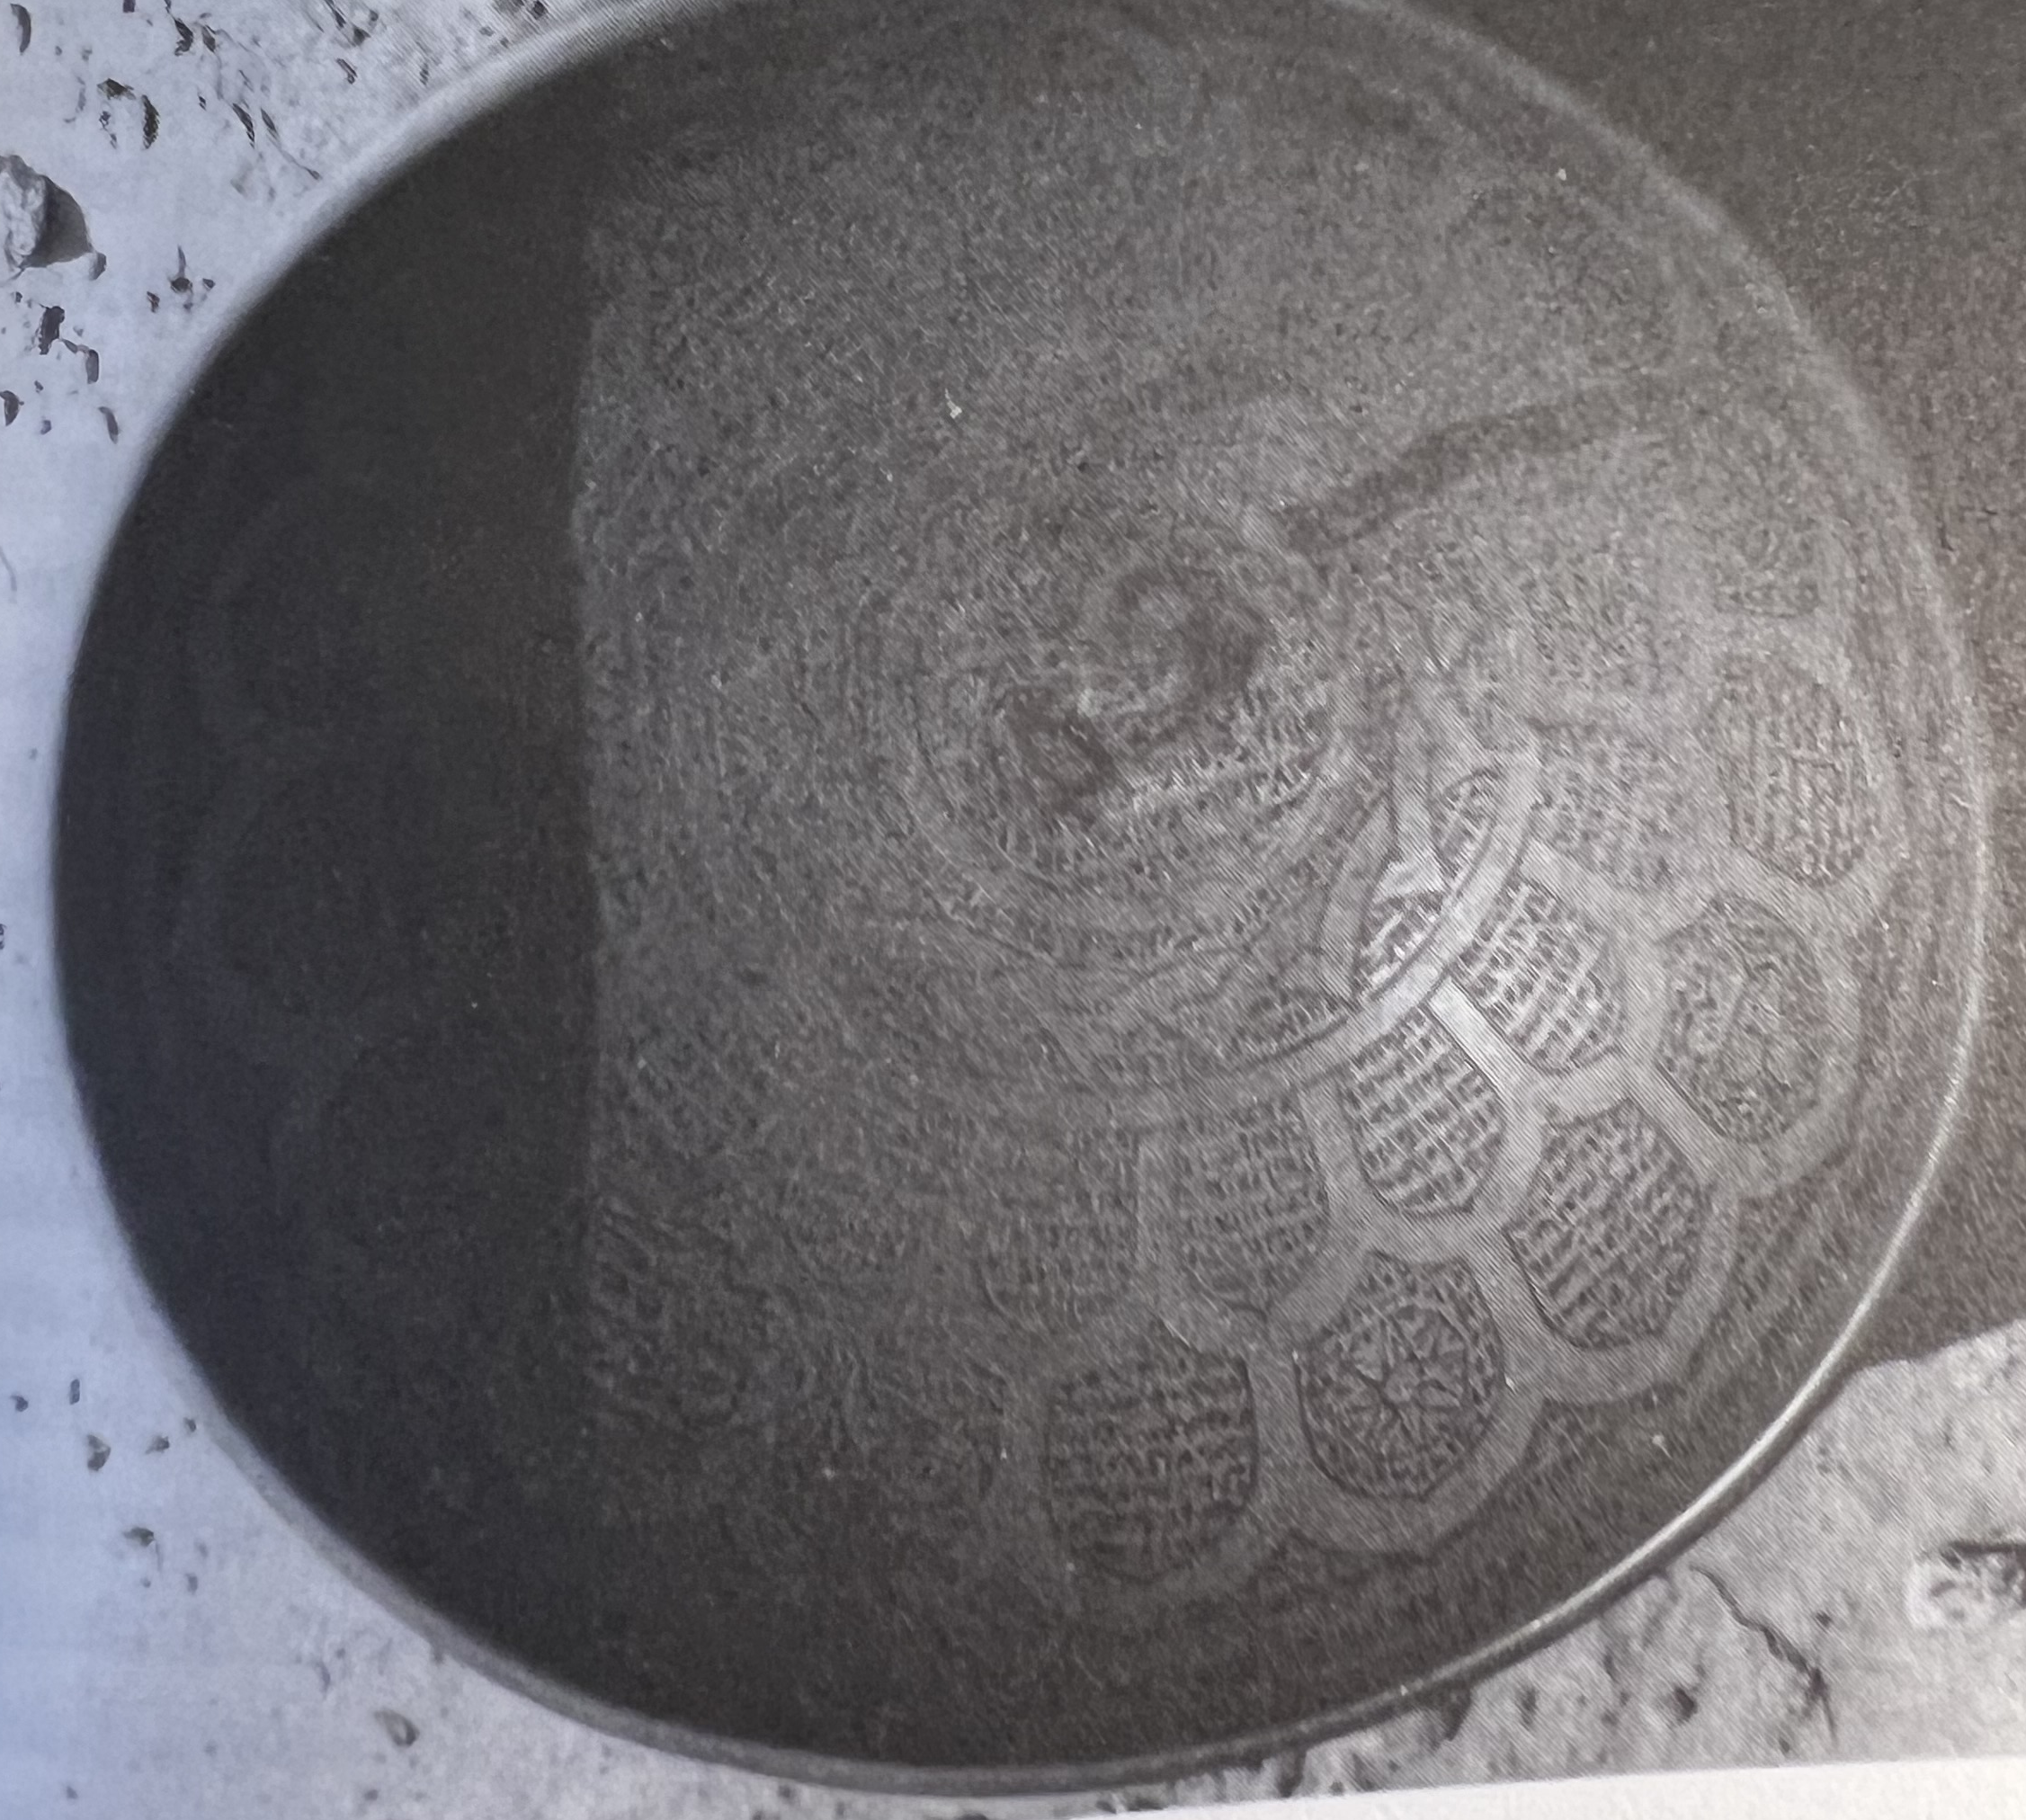
\includegraphics[width=0.6\textwidth]{HommeetIslam/Images/IMG_2457recadre.png}
 \caption{Coupe B  - paroi interne}
 
    \label{fig:my_label}
\end{figure}
\paragraph{D'où vient le pouvoir magique ?} La problématique est la suivante : d'où vient le pouvoir magique ? Est-il lié à l'autorité de l'officiant et de son initiation éventuelle, est-il lié au rite ? ou bien à l'objet lui-même ? Et si cela vient de l'objet lui-même, qu'est ce qui fait qu'un objet devient \textit{magique}.

Pour cela, après une introduction générale de la magie en Islam, nous suivrons la \textit{démonstration} d'Anne Regourd, en étudiant d'abord les deux coupes. Puis nous étudierons ce que recouvre précisément leur statut juridique. Dans la troisième partie, l'enquête de terrain permettra d'étudier l'utilisation pratique de ces coupes. Enfin, le texte étudié propose quelques pistes sur la fabrication des coupes, pour déterminer d'où vient le caractère magique. 

\subsection*{La magie en Islam}

\paragraph{La magie est présente dans le Coran.}  Ainsi, le Prophète est souvent présenté par ses adversaires comme \textit{sâhir}, \textit{sihr} étant la racine de "magie".  On trouve dans les gestes et paroles du Prophète les traces de ce qui deviendra plus tard la \textit{magie islamique} : l’incantation thérapeutique (\textit{ruqiya}), l’imprécation (\textit{licân}), le rite de guérison ou d’ensorcellement (\textit{sihr}), les techniques de divination (\textit{fa’l}), la croyance en les \textit{jinn} - le magicien est aussi le \textit{Majnun}, le \textit{possédé par les jinns} (\cite{Fadh_1987}). Ces pratiques et croyances avaient cours dans la société pre-islamique mais ont été légitimées dans le monde musulman par leur présence dans le Coran.
 

\paragraph{Dans la conception coranique, la magie n'est pas une disposition naturelle de l'homme} Le Coran mentionne Salomon comme magicien mais ce n'est pas lui le dépositaire, qu'il faut chercher encore plus loin dans le passé : 
\begin{singlequote}
     \textit{Sulaymân} n'a pas été mécréant, ce sont les \textit{shayâtin} (diables, satans) qui l'ont été et qui ont enseigné aux humains la magie  (2:102-La vache (Al-Baqarah))
\end{singlequote}
L'étude coranique permet d'identifier les premiers dépositaires de la magie à la ville de Babylone 
 (\cite{hames_coran_2007}). Il s'agirait donc d'une pratique d'origine mèdes, le puissant voisin arabe. 

\paragraph{Salomon est une figure de référence de la magie en Islam.} Salomon est souvent cité dans les pratiques liturgiques, en particulier par son \textit{sceau} - \emph{khâtim} un des signes magiques les plus présents sur les talismans et coupes magiques et qu'on peut observer sur les deux coupes : il s'agit d'une étoile à cinq ou six branches. Or, Salomon regroupe différentes figures d'autorité :
\begin{itemize}
    \item figure \textit{royale} 
    \item figure \textit{prophétique} (Salomon est un prophète en Islam)
    \item figure d'\textit{initié}, à travers le verset 2:102 mentionné plus haut. Or, l'initiation est constitutive de l'autorité dans l'Islam soufi.
\end{itemize}
De fait, on retrouve des dimensions magiques dans chacune de ces sphères d'autorité. Par exemple, \cite{coulon_magie_2017} mentionne l’ouvrage de magie le plus important de l’Islam médiéval, le \textit{Šams al-maʿārif wa-laṭāʾif al-ʿawārif}. Les nombreuses copies avec des dédicaces pour des personnalités de premier plan attestent du caractère politique de la magie, le souverain étant supposé avoir – dans la mesure du possible – la capacité de prévenir les sinistres.  
De même, l'Islam soufi a pu développer en Afrique les \textit{marabouts}, religieux mystiques jouant à la fois les rôles de prédicateur et de sorcier-thaumaturge. 

Cette brève introduction permet de souligner que les pratiques magiques ne sont pas un apport récent et exogène de l'Islam, comme le soutiennent les tenants du wahhabisme même si leur statut paraît 
ambigu dès le départ. 

Face à cette accusation récente d'illégitimité de toute magie en Islam\sn{cf ce commentaire sur Wikipedia à l'article Soufisme - version du 21 décembre 2022 : \begin{singlequote}
    les marabouts [\ldots] enseignent l'islam classique non sans lui ajouter des pratiques populaires et superstitieuses, voire magiques, rejoignant parfois des croyances animistes traditionnelles de l'Afrique.
\end{singlequote}}, il est donc intéressant d'étudier  la pratique ancienne de ces rites avec un regard d'anthropologue, et ceci non pas dans une zone "périphérique" du monde musulman mais au contraire dans une zone anciennement islamisée comme le Yémen.


\subsection*{Deux coupes magico-thérapeutiques au Nord-Yémen}

Anne Regourd s'intéresse à deux coupes qui sont la propriété d'une fondation religieuse, en pratique une mosquée du Nord-Yémen.
\paragraph{Les coupes possèdent de nombreuses références magiques.}
Les deux coupes sont en alliage cuivreux (référence coranique à Salomon, cf 34:12-13). Elles  sont recouvertes de bâtonnets "magiques" et de sceaux de Salomon, dont nous avons souligné la présence courante sur les objets magiques. Les écritures porteuses de puissances magiques sont très strictement délimitées dans des formes, une pratique courante en islam arabe. 
\paragraph{Les coupes ont une vocation thérapeutique.}  Elles sont constituées d'éléments thérapeutiques comme les sourates du Coran associées à la guérison (de la déchirure, la Répudiation,...),  et le dessin d'animaux dangereux (serpents, scorpions,...).  Les coupes ont été beaucoup utilisées (avec de nombreuses réparations). L'enquête de terrain nous indique qu'elles sont utilisés en cas d'empoisonnement ou d'accouchement difficile, et le rite est basé sur l'absorption d'un liquide par le malade.


\paragraph{L'auteure propose une lecture cosmique des coupes.}  Plusieurs éléments viennent soutenir une telle proposition et en particulier le rapport au Soleil. En effet, le chiffre 8  revient régulièrement (16 médaillons sur deux cercles concentriques sur la coupe B, 8 sceaux de Salomon sur la coupe A,...). Or, ce chiffre correspond en science des lettres à la valeur  du \textit{hâ}, lui-même clé de la vie (\textit{hayât}). Par ailleurs, les versets des médaillons rappellent que Dieu est la \textit{lumière des cieux}. 
Ce monde clos du Cosmos serait ainsi représenté : 

\begin{figure}[h!]
    \centering
     
\includegraphics[width=0.7\textwidth]{HommeetIslam/Images/IMG_2459recadre.png}
   \caption{La Coupe comme représentation du cosmos. Coupe B paroi Interne et externe}
    \label{fig:my_label}
\end{figure}
 
\subsection*{Des biens d'une fondation pieuse - \textit{waqf}}
Après avoir étudié la coupe proprement dite, l'auteure étudie le statut particulier de ces coupes : elles sont la propriété d'une fondation pieuse, \textit{waqf}, depuis 1895. Pratiquement, il s'agit d'un \textit{waqf} oral, non enregistré auprès des autorités à la différence des biens immobiliers.
En étant \textit{waqf}, la légitimité religieuse est
renforcée. 
Mais ce qui retient l'attention, c'est le faible empressement de l'intendant de la mosquée envers les 2 coupes, dont il est pourtant le gestionnaire. Il les prête gratuitement quand on les lui demande mais il peut même douter de leur efficacité. Le pouvoir magique ne vient donc pas du propriétaire et de ses références magiques (à aucun moment la compétence magique n'est requise pour être responsable de mosquée) mais bien des coupes elles-mêmes,  du rite autour de ces coupes, ou de l'artisan qui les a fabriquées. Ceci est confirmé par le fait que de telles coupes étaient offertes en cadeau, au retour du pèlerinage à La Mecque (Canaan 1923, 130 \cite[note 63]{Regourd_2007}); la coupe (A) aurait ainsi été donnée en \textit{waqf} par un \textit{hâjjî}.

\subsection*{Utilisation des coupes}
L'enquête de terrain permet de décrire l'utilisation de ces coupes, en particulier dans le cas de grossesse difficile. 

\paragraph{Leur mode d’emploi consiste principalement à boire un liquide au contact de la coupe.}  Ce liquide - de
l’eau, du bouillon - ou le miel que l’on y a versé, est bu en disant des louanges à Dieu.
Le bouillon de viande est particulièrement prescrit pour les femmes en couches : par son pouvoir nutritif important (moelle,...), il présente des caractéristiques médicales intéressantes,  qui
viennent en addition de celles des écrits et représentations présents sur les coupes. 
\paragraph{La maladie est interprétée comme la conséquence de causes multiples.} Un tel recours simultané à plusieurs médecines différentes est courant dans la même région du Yémen. Il s'agit d'attaquer le mal dans toutes ses facettes. Lorsqu’il y a maladie,
elle est toujours soupçonnée d’être le résultat de causes multiples et la boisson dans la coupe est envisagée en complément d'autres actions, en fonction du diagnostic thérapeutique. De même, l’utilisation des coupes comme réceptacle de boisson n'est pas envisagée comme l'unique usage des coupes, comme le laisse penser les traces de bougie au fond de la coupe B. 


\subsection*{Historique des coupes}
Une coupe, même abîmée, conserve ses propriétés comme c'est le cas de la coupe B réparée plusieurs fois et qui a perdu une partie de ses écrits; le rite, nous l'avons vu, est des plus simples et ne semble pas complètement fixé. D'où vient donc le pouvoir magique de ces objets ? 

Il nous faut donc étudier l'origine de ces objets, que ce soit leur commanditaire ou l'artisan qui l'a fabriqué.

\paragraph{La titulature de Saladin présente sur les coupes est apocryphe.} Le commanditaire de ces coupes serait Saladin, une titulature clairement apocryphe et commune dans les objets magiques. Par une telle référence, la légitimité du pouvoir magique se trouve renforcée. 

 


\paragraph{Le rôle de l'artisan est secondaire.} Nous n'avons pas d'informations sur l'artisan mais l'étude des diverses coupes magiques montre des artisans différents, certains excellents, d'autres se contentant de copies mais toujours avec des variantes. 
Selon les mentions de certaines coupes, la puissance magique viendrait ou serait renforcée par la survenance d'un évènement astral lors de la fabrication de l'objet. Une telle mention, doublée parfois du nom d'un souverain,  ajoute par sa simple évocation, à la valeur et l'efficacité de la coupe.  
\paragraph{L'homme s'approprie la magie d'origine divine.} Nous avons vu que dans la vision coranique, la magie n'est pas innée pour l'homme.
Un mythe d’origine
des coupes véhicule l’idée que la copie peut avoir autant d’effet que
l’original. Les Palestiniens expliquent
ainsi l'origine des coupes : les bons anges en employaient de semblables
pour faire leurs ablutions. Ils en oublièrent un jour quelques exemplaires
à côté de la source où ils avaient 1'habitude de se rassembler pour se
laver. Un homme passant par là les trouva et s'en empara. Les propriétés
miraculeuses de la coupe furent bientôt découvertes. Des copies en furent
réalisées, qui manifestèrent les mêmes propriétés (Canaan, 1923,130;
1936, 127 cité par \cite{Regourd_2007})

 

 \subsection*{Conclusion}

\paragraph{La source de la magie semble l'addition de plusieurs facteurs } A la fin de cette étude, le pouvoir de ces coupes semble venir de l'addition de plusieurs facteurs et non d'un seul : mythe originel lié aux anges, titulature de Saladin, caractères magiques, formules coraniques adaptées, animaux et sceaux de Salomon, bien \textit{waqf}. 
De la même façon, son utilisation sera complétée d'autres approches thérapeutiques pour une approche que l'on qualifierait aujourd'hui d'\textit{holistique}.

\paragraph{L'anthropologie éclaire l'islamologie} En guise de conclusion, nous essayons de penser les conséquences de cette recherche anthropologique pour l'islamologie. Il apparaît de l'étude des diverses coupes que la magie n'est pas uniquement un élément exogène ajouté  à la foi musulmane mais fait du Coran une réalité bien plus riche qu'un simple livre à lire et à étudier, avec une lecture littérale du verset  : 
\begin{quote}
    Nous envoyons du Coran ce qui est une guérison et une miséricorde pour les croyants. (17:82)
\end{quote}
\vspace{1cm}
Développant ce verset, Winter peut conclure : 
\begin{singlequote}
    This healing
power of the revelation is understood literally by many, not just spiritually.
The qur’an was thus sometimes also used physically for curing [\ldots]. By means of amulets,
talismanic shirts and other artefacts covered with qur’anic inscriptions, often
in conjunction with astrological or magical devices or practices, the revelation
came to be put to all kinds of uses, not always strictly orthodox. By procedures reminiscent of the Cabbala, the letters of the Arabic alphabet and their
numerical values themselves played an important role in Muslim mysticism,
esotericism and the divinatory arts. \cite{winter_cambridge_2008}
\end{singlequote}
 
 
 
   \chapter{coupes divinatoires}

Deux bols magique en cuivre et laiton XIXe
\paragraph{COUPE DIVINATOIRE} dit bol \textit{magique} en alliage de cuivre partiellement étamé, de forme circulaire aux bords évasés. La paroi extérieure est gravée d'une fleur de lotus à huit pétales calligraphiés au coeur en forme d'une étoile à cinq branches, et une longue inscription le long du rebord externe. L'intérieur est décoré d'un cartouche inscrit, de deux motifs de tughra, d'un sceau de propriétaire en forme d'amande «sahib Tador (Théodore ?) «et d'un cachet ARMENIEN daté 1875». Le rebord est gravé d'une longue frise épigraphique sur deux lignes. Empire ottoman, datée 1875.
Haut. : 4,9 ; Diam. : 15,1 cm

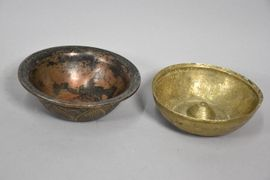
\includegraphics[]{GénéralISTR/Image/bolsmagiques.jpeg}

\includegraphics[]{}


\paragraph{Bol talismanique ou bol magique} coupe de forme circulaire à bords évasés, ombiliquée en laiton anciennement étamé incrustation de pâte noire gravé à l'intérieur de mihrabs, inscriptions en écriture naskh\sn{Le naskh, aussi appelé naskhi ou neskhi  est le style d'écriture le plus répandu pour les langues utilisant l'alphabet arabe. C'est ce style que l'on apprend à l'école et que l'on emploie pour la calligraphie et l'écriture usuelle, manuscrite ou imprimée.} et nasta'liq\sn{Le nastaliq    est un des styles de la calligraphie persane, en alphabet persan, dont l'origine est attribuée à Mir Ali Tabrizi, originaire de Tabriz, au xive siècle} d'invocation religieuse et verset coranique, patine d'usage. Iran XIX-XXe.
Haut. : 4 ; Diam. : 13,5 cm
\chapter{coupes divinatoires}



 

\section{Annexe : références}


\subsection{Coupes achetées}


\paragraph{Coupe divinatoire} dit bol \textit{magique} en alliage de cuivre partiellement étamé, de forme circulaire aux bords évasés. La paroi extérieure est gravée d'une fleur de lotus à huit pétales calligraphiés au coeur en forme d'une étoile à cinq branches, et une longue inscription le long du rebord externe. L'intérieur est décoré d'un cartouche inscrit, de deux motifs de tughra, d'un sceau de propriétaire en forme d'amande «sahib Tador (Théodore ?) «et d'un cachet ARMENIEN daté 1875». Le rebord est gravé d'une longue frise épigraphique sur deux lignes. Empire ottoman, datée 1875.
Haut. : 4,9 ; Diam. : 15,1 cm
\begin{figure}[h!]
    \centering
        \sidecaption{Coupes divinatoires}
 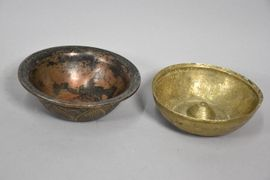
\includegraphics[width=\textwidth]{GénéralISTR/Image/bolsmagiques.jpeg}

%
\includegraphics[]{GénéralISTR/Image/Tughra_of_Abdülaziz 1861-76.jpeg}

    \label{fig:my_label}
\end{figure}


\paragraph{fleur de lotus} Dans le bouddhisme, le lotus est associé à la pureté, à l’éveil spirituel et à la fidélité. La fleur est considérée comme pure car elle est capable de sortir des eaux troubles le matin et d’être parfaitement propre. Il est également connu pour symboliser la pureté de la parole, du corps et de l’esprit.


\paragraph{Bol talismanique ou bol magique} coupe de forme circulaire à bords évasés, ombiliquée en laiton anciennement étamé incrustation de pâte noire gravé à l'intérieur de mihrabs, inscriptions en écriture naskh\sn{Le naskh, aussi appelé naskhi ou neskhi  est le style d'écriture le plus répandu pour les langues utilisant l'alphabet arabe. C'est ce style que l'on apprend à l'école et que l'on emploie pour la calligraphie et l'écriture usuelle, manuscrite ou imprimée.} et nasta'liq\sn{Le nastaliq    est un des styles de la calligraphie persane, en alphabet persan, dont l'origine est attribuée à Mir Ali Tabrizi, originaire de Tabriz, au xive siècle} d'invocation religieuse et verset coranique, patine d'usage. Iran XIX-XXe.
Haut. : 4 ; Diam. : 13,5 cm


\paragraph{Classical Islamic Theology}\sn{Tim Winter. The Cambridge Companion to Classical Islamic Theology (Cambridge Companions to Religion) (pp. 188-189). Cambridge University Press. Édition du Kindle. } \cite{winter_cambridge_2008}
\begin{quote} 
    That its signifier is such an important part of its signified contributes in making the Qur’an a much richer reality than a mere book to be read and studied. Of course, even before being a scripture, the revelation sent down to Muammad is a speech. And as God Himself explains, the words of this speech operate in many ways. They are not supposed to affect minds only. “They only are the believers whose hearts tremble with fear when God is mentioned. When His verses are recited to them, they make their faith increase and they put their trust in their Lord” (8:2). “When the verses of the Compassionate are recited to them, they fall down in prostrate adoration, weeping” (19:58). “God has sent down the most beautiful speech as a Scripture … whereat the skins of those in awe of their Lord shiver, and then their skins and their hearts soften to God’s remembrance” (39:23). “We send down, as the Qur’an, something that is a healing and a mercy for the believers” (17:82). This healing power of the revelation is understood literally by many, not just spiritually. The qur’an was thus sometimes also used physically for curing ailments: a piece of paper with a qur’anic inscription was dipped into water; once the ink was diluted, the qur’anically enriched water was drunk. By means of amulets, talismanic shirts and other artefacts covered with qur’anic inscriptions, often in conjunction with astrological or magical devices or practices, the revelation came to be put to all kinds of uses, not always strictly orthodox. By procedures reminiscent of the Cabbala, the letters of the Arabic alphabet and their numerical values themselves played an important role in Muslim mysticism, esotericism and the divinatory arts. This is particularly true of the seventy-eight “mysterious” letters opening twenty-nine of the qur’anic sūras (2–3, 7, 10–15, 19–20, 26–32, 36, 38, 40–6, 50, 68) and which, once they are reduced to the fourteen of which they are combinations, represent the various basic consonantal forms of written Arabic, hence of the whole Arabic alphabet.11 The fact that through qur’anic psalmody and calligraphy the most manifest ways of celebrating God’s revelation have given rise to arts that are among the most representative of Islam, if not the two major Islamic arts, is also to be explained as an aspect of what the Algerian Malek Bennabi rightly called “the Qur’anic phenomenon”. Be it through architecture, decorative arts, the media or other aspects of everyday life, the divine revelation conveyed in Arabic by the Prophet continues to be as present in the public sphere as it is in the hearts of the millions of those who, in their childhood, learn it by heart, often entirely. And just as Arabic is per se part of the Qur’an, the latter impregnates it to the point of making it impossible for non-Muslim Arabic-speakers not to be, in some way, linguistically Islamised.
 


\end{quote}


\begin{quote}
    La mise en scène du pouvoir au Moyen Âge confère aux souverains une autorité de nature quasi magique. Aziz Al-Azmeh dépeint ainsi la figure idéale de
l’homme de pouvoir dans l’Islam médiéval :
\begin{quote}
    Au niveau le plus élémentaire, n’importe qui aurait commencé avec les
qualités quasi-magiques de la personne du calife. Il y a un propos, très
répandu dans les écrits arabes médiévaux et attribué à la sagesse persane,
selon lequel la justice d’un roi – sulṭān, un terme fréquemment appliqué
aussi aux califes – garantit le bon fonctionnement des saisons, la
pluviosité et l’irrigation idoine, la bonne reproduction du bétail et le fonctionnement
correct du commerce. Cette indication n’est pas simplement
réductible à une expression sur les connections structurales du monde de
la prospérité détaillée dans le ‘cercle de justice’ étudié dans le précédent
chapitre, mais a des interprétations au-delà et en-deça de celles de la sagesse
politique et des conseils généraux aux rois. Il était perçu comme une
manifestation empirique que l’injustice royale ne produit pas seulement
des effets matériels délétères, mais suscite des forces surnaturelles qui
agissent ineffablement, à une certaine distance, en faisant arrêter le ciel
de pleuvoir et le bétail de se reproduire. Les effets naturels de l’injustice
royale ne sont pas simplement métaphoriques, parce qu’ils ont à faire 
 avec la baraka selon deux aspects alambiqués : la baraka obtenue avec la
justice, qui se tarit avec l’injustice. La baraka était bien sûr partagée avec
les cheikhs soufis et les saints ḥanbalites. De nombreux actes et capacités
merveilleux et tangibles étaient attribués à Aḥmad b. Ḥanbal et d’autres ;
\end{quote}


mais ceux-ci étaient aussi recherchés du lointain calife1.
Ainsi les sujets étaient en droit d’attendre la justice du pouvoir politique, et
la justice est elle-même une condition préalable pour la bénédiction dont
peuvent bénéficier les sujets. Le souverain devait rivaliser avec les saints en
justice et en bienveillance. Il était supposé avoir – dans la mesure du possible –
la capacité de prévenir les sinistres. L’intérêt des cours pour la magie et la divination
avait une réelle signification politique. L’existence de copies du Šams
al-maʿārif dédicacées à des figures politiques, comme nous allons le voir, est un
indicateur important dans cette perspective.\cite{coulon_magie_2017}
\end{quote}
\paragraph{Duquoc} Nous nous trouvons là devant une ferme conviction :

\begin{quote}
    « Jésus ne se replie pas sur l’instant, il l’ouvre à sa profondeur », car le présent est « l’habitat de Dieu » (p. 113).
\end{quote} 
L’auteur revient sur ce point avec insistance, comme pour surmonter le caractère paradoxal des affirmations du Christ, puisque si le Règne est là, le mal et l’injustice, eux aussi, semblent continuer de régner, inexorablement. La « tentation » est alors grande de vouloir faire coïncider le Règne présent avec la fin d’une histoire réconciliée qui dénie les réalités de notre histoire souffrante, en faisant appel à la \textbf{magie}, à la puissance messianique, à la conquête instaurant de force l’unité du Règne promis (comme le suggère le tentateur à Jésus au seuil de sa mission). L’Église n’a pas toujours résisté à cette tentation, comme on le voit lorsqu’elle cherche à dominer et à orienter la politique, illusion dénommée chrétienté (l’auteur développe ici sa réflexion en tirant profit du livre de Marcel Gauchet : La religion dans la démocratie. Parcours de la laïcité, Gallimard, Paris, 1998).  

\subsection{Dictionnaire sociologie religions}

 \paragraph{du prophétisme }
 
Du latin divinatio, deviner, le terme « divination » désigne l'action qui se donne pour objectif de deviner, prévoir et/ou influencer une réalité cachée, à l'aide de la lecture d'éléments, ou présages, selon une technique particulière impliquant leur observation ou leur manipulation. Ainsi définie, la divination apparaît comme une pratique universelle des sociétés  Les procédures divinatoires peuvent être motivées par diverses raisons découvrir les causes d'une maladie ou d'une infortune, retrouver un objet perdu, connaître les déterminations pesant sur l'avenir proche (dans le domaine de l'amour, du travail, etc.), être informé des circonstances propices à la réalisation d'une action ainsi que de ses chances de succès (départ à la guerre ou à la chasse, construction d'une maison, installation sur un territoire, etc.). La divination peut aussi être exécutée de manière quasi automatique, parce qu'elle est requise en telle circonstance par la tradition ou qu'elle fait partie intégrante d'un rituel. La divination est, soit explicative   et renvoie alors à des éléments passés, soit prédictive permettant de
connaître l'avenir de sorte à agir en conséquence. Elle peut être réalisée pour le compte d'un individu, d'un groupe, ou d'un « bien » (du bétail, par exemple).
Les éléments qui servent de présages sont variés et leur lecture est susceptible d'être effectuée selon des procédés très divers : observations et/ou manipulations d'entrailles d'animaux sacrifiés, de vols d'oisceaux, de craquelures sur une carapace de tortue calcinée, de marc de café, de combinaisons d'objets lancés, de cartes, de présence de taches dans un jaune d'œuf, de l'emplacement des planètes, etc. Cette multiplicité des techniques s'illustre par la diversité des termes formés à partir de la racine grec \textit{mantiké} -divination-pour les désigner : chiromancie, géomancie, cartomancie, etc. La divination peut aussi être opérée sans autre support que le devin lui-même. Elle s'inscrit alors plutôt dans le domaine de la voyance : le devin établit un contact qui est dit direct -via les rêves, la transe ou la possession- avec des forces sur-naturelles. Mais si de multiples classifications des formes de divination ont été proposées formes ou techniques intuitives, inspirées, inductives, raisonnées..), aucune n'apparaît universellement pertinente, et il semble plus utile de se référer aux classifications indigènes
- les modes de divination étant généralement pluriels dans une même société.

\paragraph{Hasard exclu des évènements}
En se fondant sur la combinaison, qui
nés à semble résulter du hasard, des éléments qui tion- servent de présages, la procédure divinatoire incie, manipule l'aléatoire pour mieux le dépasser.
si être
Une signification étant attribuée à chacune
 des combinaisons possibles. le hasard est   exclu de la trame des événements. L'incertitude qui motive la divination se trouve alors   intégrée dans un ordre intelligible et
  rassurant.

 le cours du destin peut toujours être plus ou moins « forcé ». Les processus divinatoires prédictifs servent d'ailleurs souvent à se prémunir contre un événement futur potentiel, voire à créer un autre futur : il est fréquent de recommencer une divination jusqu'à obtenir le résultat escompté, comme s'il s'agissait de mettre en place les conditions propices à la réussite de l'action que l'on souhaite entre-prendre. De ce fait, la divination intéresse les réflexions sur les processus de prise de décision et les théories de l'action. Entérinant certaines formes d'actions, elle œuvre comme une procédure de validation, ce qui la rapproche des systèmes juridiques.
\paragraph{Individuel et social}
La divination relève en fin de compte autant de l'individuel que du social. Elle est le résultat d'une interaction, impliquant au minimum le devin et son client, et généralement tout un pan de la société. En inscrivant le destin individuel dans un ordre englobant, les processus divinatoires font de l'individu un élément d'un système socio-cosmique qui le dépasse. Entre l'individu et le social, l'aléatoire et la détermination, l'interprétation et l'action, le religieux et le juridique, les processus divinatoires, variés dans leurs formes et leurs fonctions, touchent à de nombreux aspects de la vie d'une société, qu'ils permettent d'articuler.

\paragraph{bibliographie}
\begin{itemize}
    \item ADLER A. et ZEMPLENI A., Le Bâton de l'aveugle : divination, maladie et pouvoir chez les Moundang du Tchad, Paris, Hermann « Savoir », 1972.   
    \item  CAQUoT A.
et LEIBOVICI M. (éds), La Divination, Paris, PUF,
1968. - EVANS-PRITCHARD E. E., Sorcellerie, oracles et magie chez les Azandé (1937), traduction ft. L.
 Evrard, Paris, Gallimard, 1972. 

  \item  FAHD T., La Divination arabe: études religieuses, sociologiques et folkloriques sur le milieu natif d'Islam, Leyde, Brill, 1966. \href{https://books.google.fr/books?id=ETsVAAAAIAAJ&lpg=PP1&hl=fr&pg=PA8#v=onepage&q&f=false}{La divination Arabe}
  \item  MAUPOIL B., La Géomancie à l'ancienne côte des esclaves, Paris, Institut d'Ethnologie, 1941, - PEEK P.-
M., African Divination Systems: Ways of Knowing.
Bloomington, Indiana University. Press, 1991.
  \item  VERNANT J.-P, VANDERMEERSCH L.. GERNET J., BOTTERO J. et al, Divination et rationalité, Paris, Seuil « Recherches Anthropologiques », 1974.
 
\end{itemize}

 



 
\section{Deux coupes magico-thérapeutiques, biens de fondation pieuse (Nord du Yémen) : transmission du savoir et efficacité}

\paragraph{tâsa, coupes magico-thérapeutiques}
\mn{\href{http://www.anne.regourd.org/arb2/wp-content/ar/docs/RegourdA_CoupesMagicoTherapeutiquesYemen-ocr.pdf}{Deux coupes magico-thérapeutiques, } biens de fondation pieuse (Nord du Yémen): transmission du savoir et efficacité - Anne REGOURD}
 \paragraph{Deux coupes, biens de fondations religieuses}
Deux coupes magico-thérapeutiques (sing. \textit{tâsa}) sont dites biens de fondation pieuse ({\textit{waqf}}) d'une mosquée, à Sanaa. Elles appartiennent à une collection d'objets, tous ayant le même statut juridique et tous utilise à des fins thérapeutiques. La famille du responsable de l'intendance à la mosquée, a la garde de ces objets et doit les remettre à quiconque les réclame dans un dessein, bien sûr, thérapeutique. Le statut juridique précis de ces objets, inédit, soulève de nombreuses questions, et, en particulier, pour le domaine ici couvert, celle de savoir ce qui les rend efficaces.
Afin de me situer dans le cadre thématique de cet ouvrage, je me pencherai sur les différentes inscriptions, représentations et figures géométriques gravées sur les parois des deux coupes. Différentes réflexions sur l'usage et la fabrication des coupes en général, à partir des travaux existants, amèneront à se demander dans quelle mesure il est possible de parler de «coupes talismaniques ».
Cette étude a fait l'objet d'un terrain entre les années 1995 et 1998.
Nous ne disposons que de peu de descriptions de coupes se trouvant au Yémen ou ayant un lien avec ce pays, par rapport à la quantité d importante de travaux publiés sur ces objets.
\subsection{Description des coupes}


\subsection{les coupes proprement dites}

\paragraph{Coupe A alliage cuivreux}
La première coupe A, hémisphérique, sans pied, à lèvre arrondie, réalisée dans un alliage cuivreux. La surélévation qu'on remarque en son centre semble résulter d'un choc. Ses dimensions, estimées d'après photo sont pour sa hauteur, de 7 à 8 cm environ, et pour son diamètre, de 15 16 cm environ*. Elle est antérieure à 1313/1895-96 (date de mise en \textit{waqf}). Elle porte sur ses parois interne et externe un décor incisé de façon assez sommaire, et a peut-être été rapportée du pèlerinage à \textit{La Mecque} par son donateur.


\paragraph{decor interne 8 entrelacs}
Le décor de la paroi interne est organisé à partir du motif central qu'orne le fond de la coupe. Il présente deux carrés entrecroisés dont les huit pointes, prolongées à 45° par des droites, se rattachent à un cercle situé quelques centimètres de la lèvre, formant ainsi un motif structurant analogue à celui d'une roue. Au centre de la coupe, dans l'espace circonscrit par les deux carrés. se trouvent. gravés sur huit lignes, des bâtonnets, isolés les uns des autres et saturant l'espace. L'espace résiduel entre les pointes et les côtés des carrés est occupé par des marques, reprenant sans doute les bâtonnets. Huit médaillons occupent le registre intermédiaire, structuré par les pointes développées des deux carrés. On distinguera quatre médaillons, dans la moitié inférieure desquels figurent des représentations animalières et, dans la moitié supérieure, des bâtonnets, semblables à ceux qui viennent d'être décrits. Ces quatre médaillons alternent avec quatre autres, comportant des textes en arabe. 
\paragraph{des animaux, scorpion, chien, dragons}
Dans le premier type de médaillon, on parvient à identifier, en ce qui concerne les animaux représentés et dans le sens des aiguilles d'une montre, un scorpion (voir flèche fig. 1, coupe A), un chien, deux dragons affrontés (?), surmontés d'une bande ondulée, et un autre quadrupède (un cheval, un lion ?), avec au-dessus du dos un \textsc{sceau de Salomon}. 
\paragraph{bâtonnets magiques}
Les bâtonnets « magiques ». quant à eux, sont chaque fois disposés sur trois lignes. Statistiquement, leur nombre est à peu près le même pour un médaillon donné : partant du scorpion et suivant le même sens, de la ligne supérieure à la ligne inférieure, on obtient le résultat suivant : 18/18/19 ; 19/19/17 ; 16/17/16 et 15/15/15.
\paragraph{des sourates, reconnues par les lettres liminaires}
Quant aux textes des médaillons, en partant de celui situé entre le scorpion et le chien (?) et en allant dans le sens des aiguilles d'un montre, on parvient à déchiffrer :
\begin{itemize}
    \item (1) la \textit{basmala}, suivie de s84v1-4 (sourate « La déchirure », a
\textit{Inshigãq}), le 4° verset s'achève à : \textit{wa algat má fihà}, puis sur la ligne
les lettres \textit{kâf-râ'} (?), et, en dessous, sìn (?)-käf.
\item (2) dans le style d'une invocation (azîma) : « yâ Nüh, Banüh, Kali
(2), Kalükh, Kalkh, \textit{alif}-lâm-mim-ra' [lettres liminaires, sourate 13], alij lâm-mîm [lettres liminaires, sourates 2, 3, 29, 30, 31 et 32], \textit{alif}-lâm-min
ra' [ibid.], \textit{hâ}'-mêm-ayn-sîn-gaf [lettres liminaires, sourate 42], kâf-\textit{hâ}
ya'-ayn-sad [lettres liminaires, sourate 19], ta' (?), tâ'-\textit{hâ} [lettres lim naires, sourate 20], ta'-\textit{hâ} (?) », enfin dernière ligne, des chiffres (?).
\item (3) ???, des lettres séparées sur les deux dernières lignes : sìn-\textit{waw} (?
mim (?), ba', puis \textit{kâf}, ra' (?).
\item (4) ???, des lettres séparées sur les deux dernières lignes : shin-ra
\textit{hâ}'-ra', \textit{alif}, \textit{hâ} (?), puis \textit{alif}, hā'-ra' , \textit{alif}, dal, \textit{alif}.
\end{itemize}

\begin{figure}[h!]
    \centering
  
    \sidecaption{Coupe A paroi intérieure, la flèche indique le scorpion}
    \includegraphics[width=\textwidth,angle=-90]{HommeetIslam/Images/IMG_2455recadre.png}
    \label{fig:my_label}
\end{figure}



\paragraph{les 7 lettres : sceau de Salomon} Ces textes sont écrits pour trois d'entre eux sur sept lignes, un seul occupe huit lignes. Enfin, le registre compris entre la lèvre de la coupe le cercle auquel se rattachent les pointes des carrés, présente, aux extrémités du cercle, 4 rectangles (façades de bâtiment, talismans?) alternant avec  4 formes cintrées (\textit{mihrabs} ou stèles funéraires, amulettes ?). Ils contiennent les mêmes bâtonnets, arrangés sur des lignes, que les médaillons animaliers. Leur nombre est à peu près constant, dans les rectangles, entre 7 et 9 par ligne, dans les formes cintrées, entre 6 et 8 par ligne. L'espace entre ces motifs est occupé en alternance par des écrits magiques et de l'arabe, placés de façon à correspondre au style des écritures contenues dans les médaillons : les écrits magiques, au-dessus des écrits magiques et l'arabe au-dessus de l'arabe. A propos des écrits magiques, on relève systématiquement la présence d'hexagrammes ou \textit{sceaux de Salomon}, suivis (dans le sens de l'écriture arabe, i. e. de droite à gauche) d'une série relativement stable de signes, de sorte que l'on a sensiblement quatre fois le même ensemble. Ces séries peuvent être assimilées à ce qu'\textit{al-Bûni} appelle les sept lettres (\textit{al-ahruf al-sabr}), ou bien les
sept sceaux (\textit{al-khawâtim al-sab}°), ou encore \textit{al-tilsam al-Sulaymani}. 

Après le sceau de Salomon, on relève successivement trois traits verticaux
surmontés d'un trait horizontal; la lettre \textit{mim} (parfois réduite à un trait sans véritable boucle, mais ce trait apparaît bien distinct des trois précédent reliés par le surlignage); deux traits verticaux, plus longs que les autre comportant deux barres obliques, qui les rendent analogues à des dièses (dans un cas sur quatre, les deux barres obliques n'apparaissent pas); quatre traits; pour conclure, une nouvelle étoile à six branches, mais aussi une sorte de y (?). La fin diffère de la série donnée par al-Bûnì, qui cite, après le quatre traits, les lettres \textit{\textit{hâ}}', puis \textit{wâw}. A moins de considérer, pour la coupe A, que la ligne qui clôt chaque série, et commence sur la ligne d'écriture revient vers le haut en s'incurvant et en direction des « lettres » précédentes ne soit un \textit{wâw} (Rehatsek, 1875b, 301, fig. 2). Chaque ensemble formé par ces « lettres » ou « sceaux » se trouve délimité par le cercle qui définit registre dans sa partie inférieure et par un surlignage plus ou moins continu qui rejoint le cercle en fin de séquence : chaque ensemble apparaît donc inscrit dans un cartouche. 
\paragraph{délimiter l'écriture magique} Le fait de délimiter un écrit porteur d'une puissance magique est une pratique courante en islam arabe. Quant aux textes en arabe, on déchiffre : 
\begin{enumerate}
 
    \item   « La basmala, suivie de trois mots (?) ;   \item  \textit{wa ma
yatawakkal'ala Allah fa-huwa} (?) ;   \item  fa-huwa [une seconde fois ?] \textit{hasbuhu inna Alläh baligh amrihi;}
\item \textit{ wa al-salâh wa al-salâm 'alâ sayyidina Muhammad}
\end{enumerate}
Les textes 2 et 3 sont tirés de s65v3 (« La Répudiation », \textit{al-talâq}). La \textit{basmala} est liminaire et la prière adressée à Dieu en faveur du Prophète Muhammad, qui vient souvent clore un écrit, se trouve dans le dernier cartouche, suivant le sens de lecture de gauche à droite. Il peut donc s'agir d'une seule et même formule qui, déroulée sur le pourtour en 4 segments, pourrait être lue perpétuellement. Cette coupe, dans sa composition interne, est, on le constate, largement construite selon le chiffre huit, souvent obtenu par l'utilisation de 4 fois 2 types d'éléments différents.
 \begin{figure}
     \centering
 
     \sidecaption{Coupe A paroi externe}
     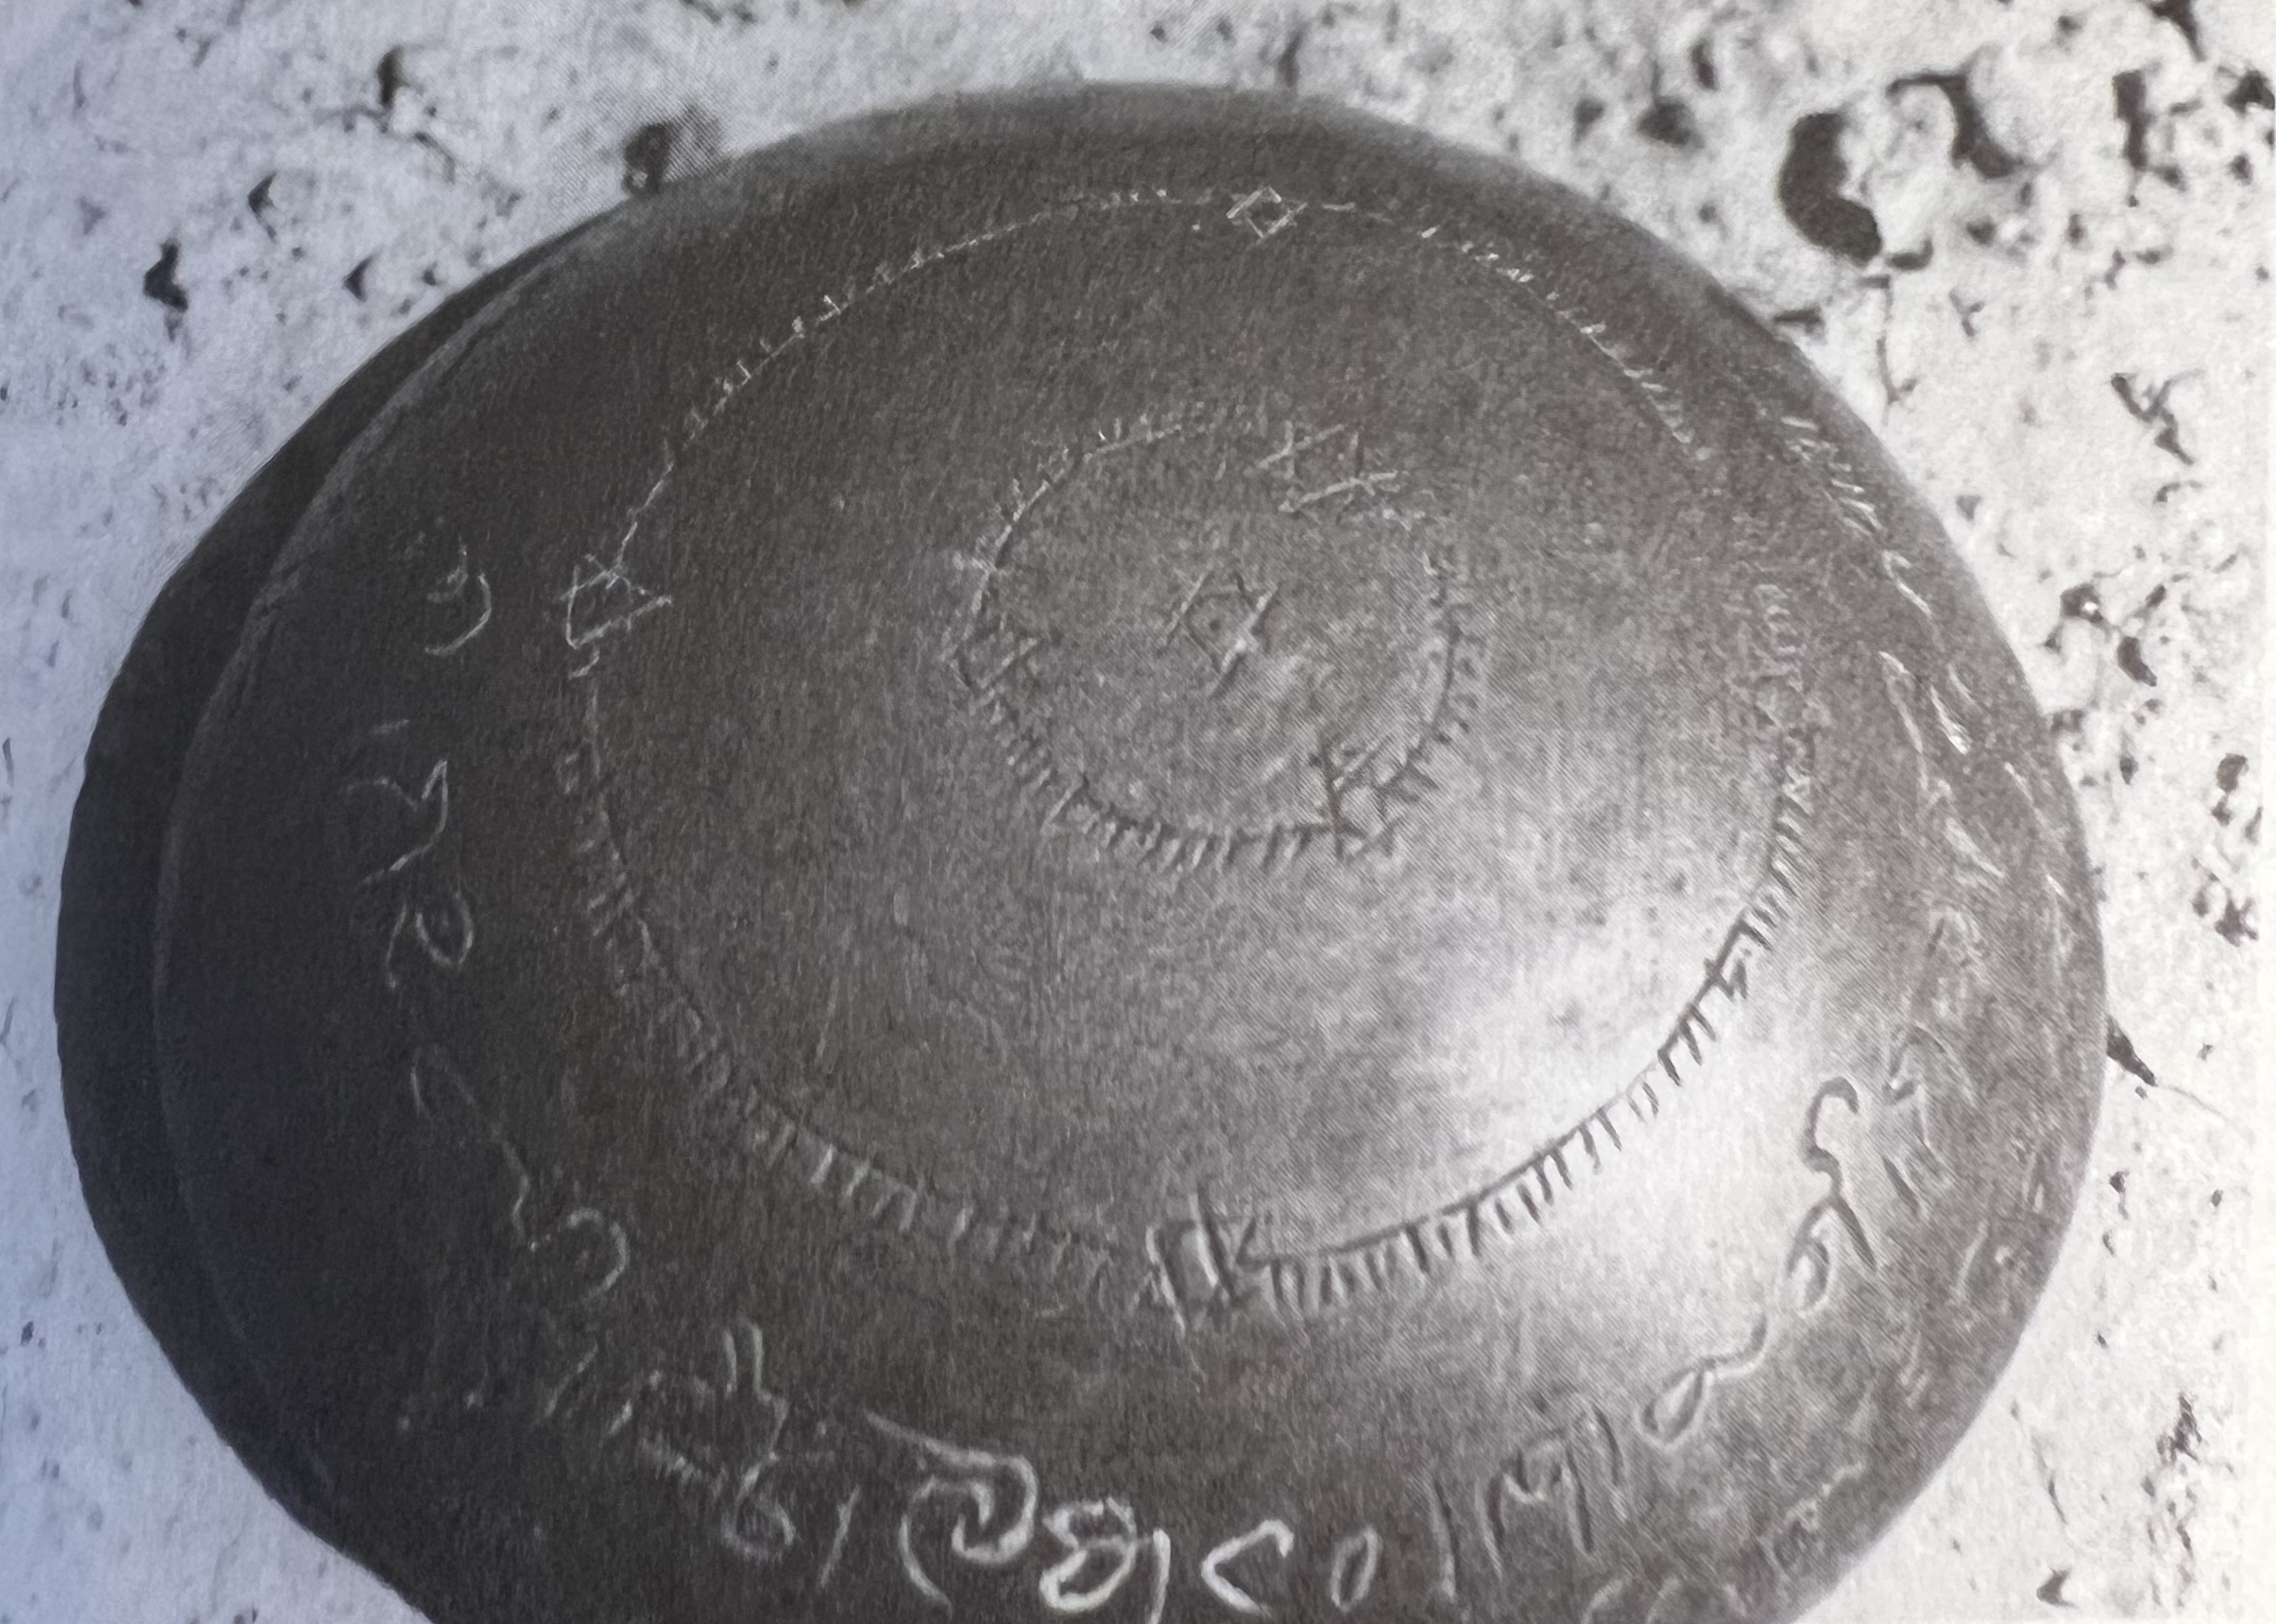
\includegraphics[width=\textwidth]{HommeetIslam/Images/IMG_2456recadre.png}
     \label{fig:my_label}
 \end{figure}

\paragraph{sceaux de salomon sur la paroi extérieure}La paroi extérieure comporte trois zones concentriques. Le fond de la coupe est occupé par un sceau de Salomon. Un premier anneau sur lequel s'alignent des bâtonnets est interrompu trois fois par des sceaux de Salomon, disposés en triangle. Un second anneau, situé dans la partie basse de la coupe, reprend le même système de bâtonnets et de sceaux, cette fois au nombre de quatre et disposés en carré. On dénombre ainsi huit sceaux de Salomon. Enfin, entre cet anneau et la lèvre, on relèvera deux lignes de texte. L'une, dont l'incision est plus profonde, se trouve gravée à proximité de la lèvre et s'étend sur tout le pourtour; elle indique :
 \begin{quote}
     « Hädhihi (2)\mn{Soit : « Celle-ci [i. e. cette coupe] [sert] pour la piga-re du serpent et du scorpion, les chiens enragés, à faciliter l'accouche. ment, aux saignements de nez, [pour les douleurs à] l'estomac ... (?), les coliques …. (?), un sceau de Salomon ... (?) »} li-lasat al-hayya wa al-agrab wa al-kalib (sic) al-kalib wo
li-usr al-walad wa al-ruäf wa al-miada ... (?) al-qawlanj ... (?) un sceau de Salomon ... (?) ».
 \end{quote}
 \paragraph{Un rajout : des objets qui vivent}Deux traits verticaux avec une barre médiane séparent le début de la fin de la phrase. L'autre inscription, située entre celle-ci et le second anneau, est incisée plus profondément, le trait en est plus épais que la précédente. Cela suggère un rajout,
le texte le confirme : 
\begin{quote}
    « Waqafa \mn{[legs pieux du Häjj Husayn al-Hawa (?) à la mosquée, la protégée, en 1313/1895-96]} al-Hajj Husayn al-Hawâ (?) \textit{hâ}dhihi al-
tâsa (sic) alâ al-Jâmi al-mahrûs 1313 »
\end{quote}   La lecture du nom du donateur pose problème, car un \textit{alif} semble avoir été tracé à la suite du \textit{hâ}', puis un \textit{waw} gravé en partie sur le \textit{alif} et avec la marque d'un rattachement à une lettre qui le précèderait, mais qui n'est pas donnée; enfin de petites encoches semblent indiquer une volonté de raturer ce \textit{waw}.
Ensuite apparaît un signe ressemblant à deux \textit{waw}-s inversés dont les boucles s'entrelacent : il peut être identifié comme une marque de fin de phrase, à la manière des petits décors que l'on trouve dans les manuscrits.

\subsection{la coupe B}
\paragraph{coupe B plus grande et ouvragée dans un alliage cuivreux}
La seconde coupe B, plus grande et plus ouvragée sur ses parois internes et externes au décor incisé, sans pied, à lèvre arrondie, a été réalisée dans un alliage cuivreux, et son fond, fendillé de manière semi-circulaire par l'usage, a fait l'objet d'une \textbf{réparation}. Il s'agit vraisemblablement d'une soudure. Ses dimensions sont de 6,5 à 6,6 cm de hauteur et de 18,3 cm de diamètre, mesuré de bord à bord extérieurs, la lèvre comptant pour 0,4 cm. Elle est de provenance inconnue. 

\paragraph{proche d'autres coupes se référant à Saladin}En ce qui concerne le décor de ses parois extérieure et intérieure, elle se rapproche d'autres coupes se référant à Abû al-Muzaffar Yûsuf (habituellement identifié comme Saladin), avec la liste de ses vertus curatives - il en sera question plus bas - mais s'en distingue, par l'absence de représentation de la Kaba en son centre (intérieur) (Savage-Smith, 1997, 73). Elle se rapproche davantage de quatre autres coupes, trois décrites par Rehatsek, et la quatrième, propriété du Science Museum à Londres. Elle n'est pas datée, mais à coup sûr fabriquée postérieurement à l'époque de Saladin,  semblablement entre le VIII-IX'/XIV°-XV° s. et le XII/XVIII, peut-être XIII /XIX s..
\begin{figure}
    \centering
       \sidecaption{Coupe B paroi interne}
 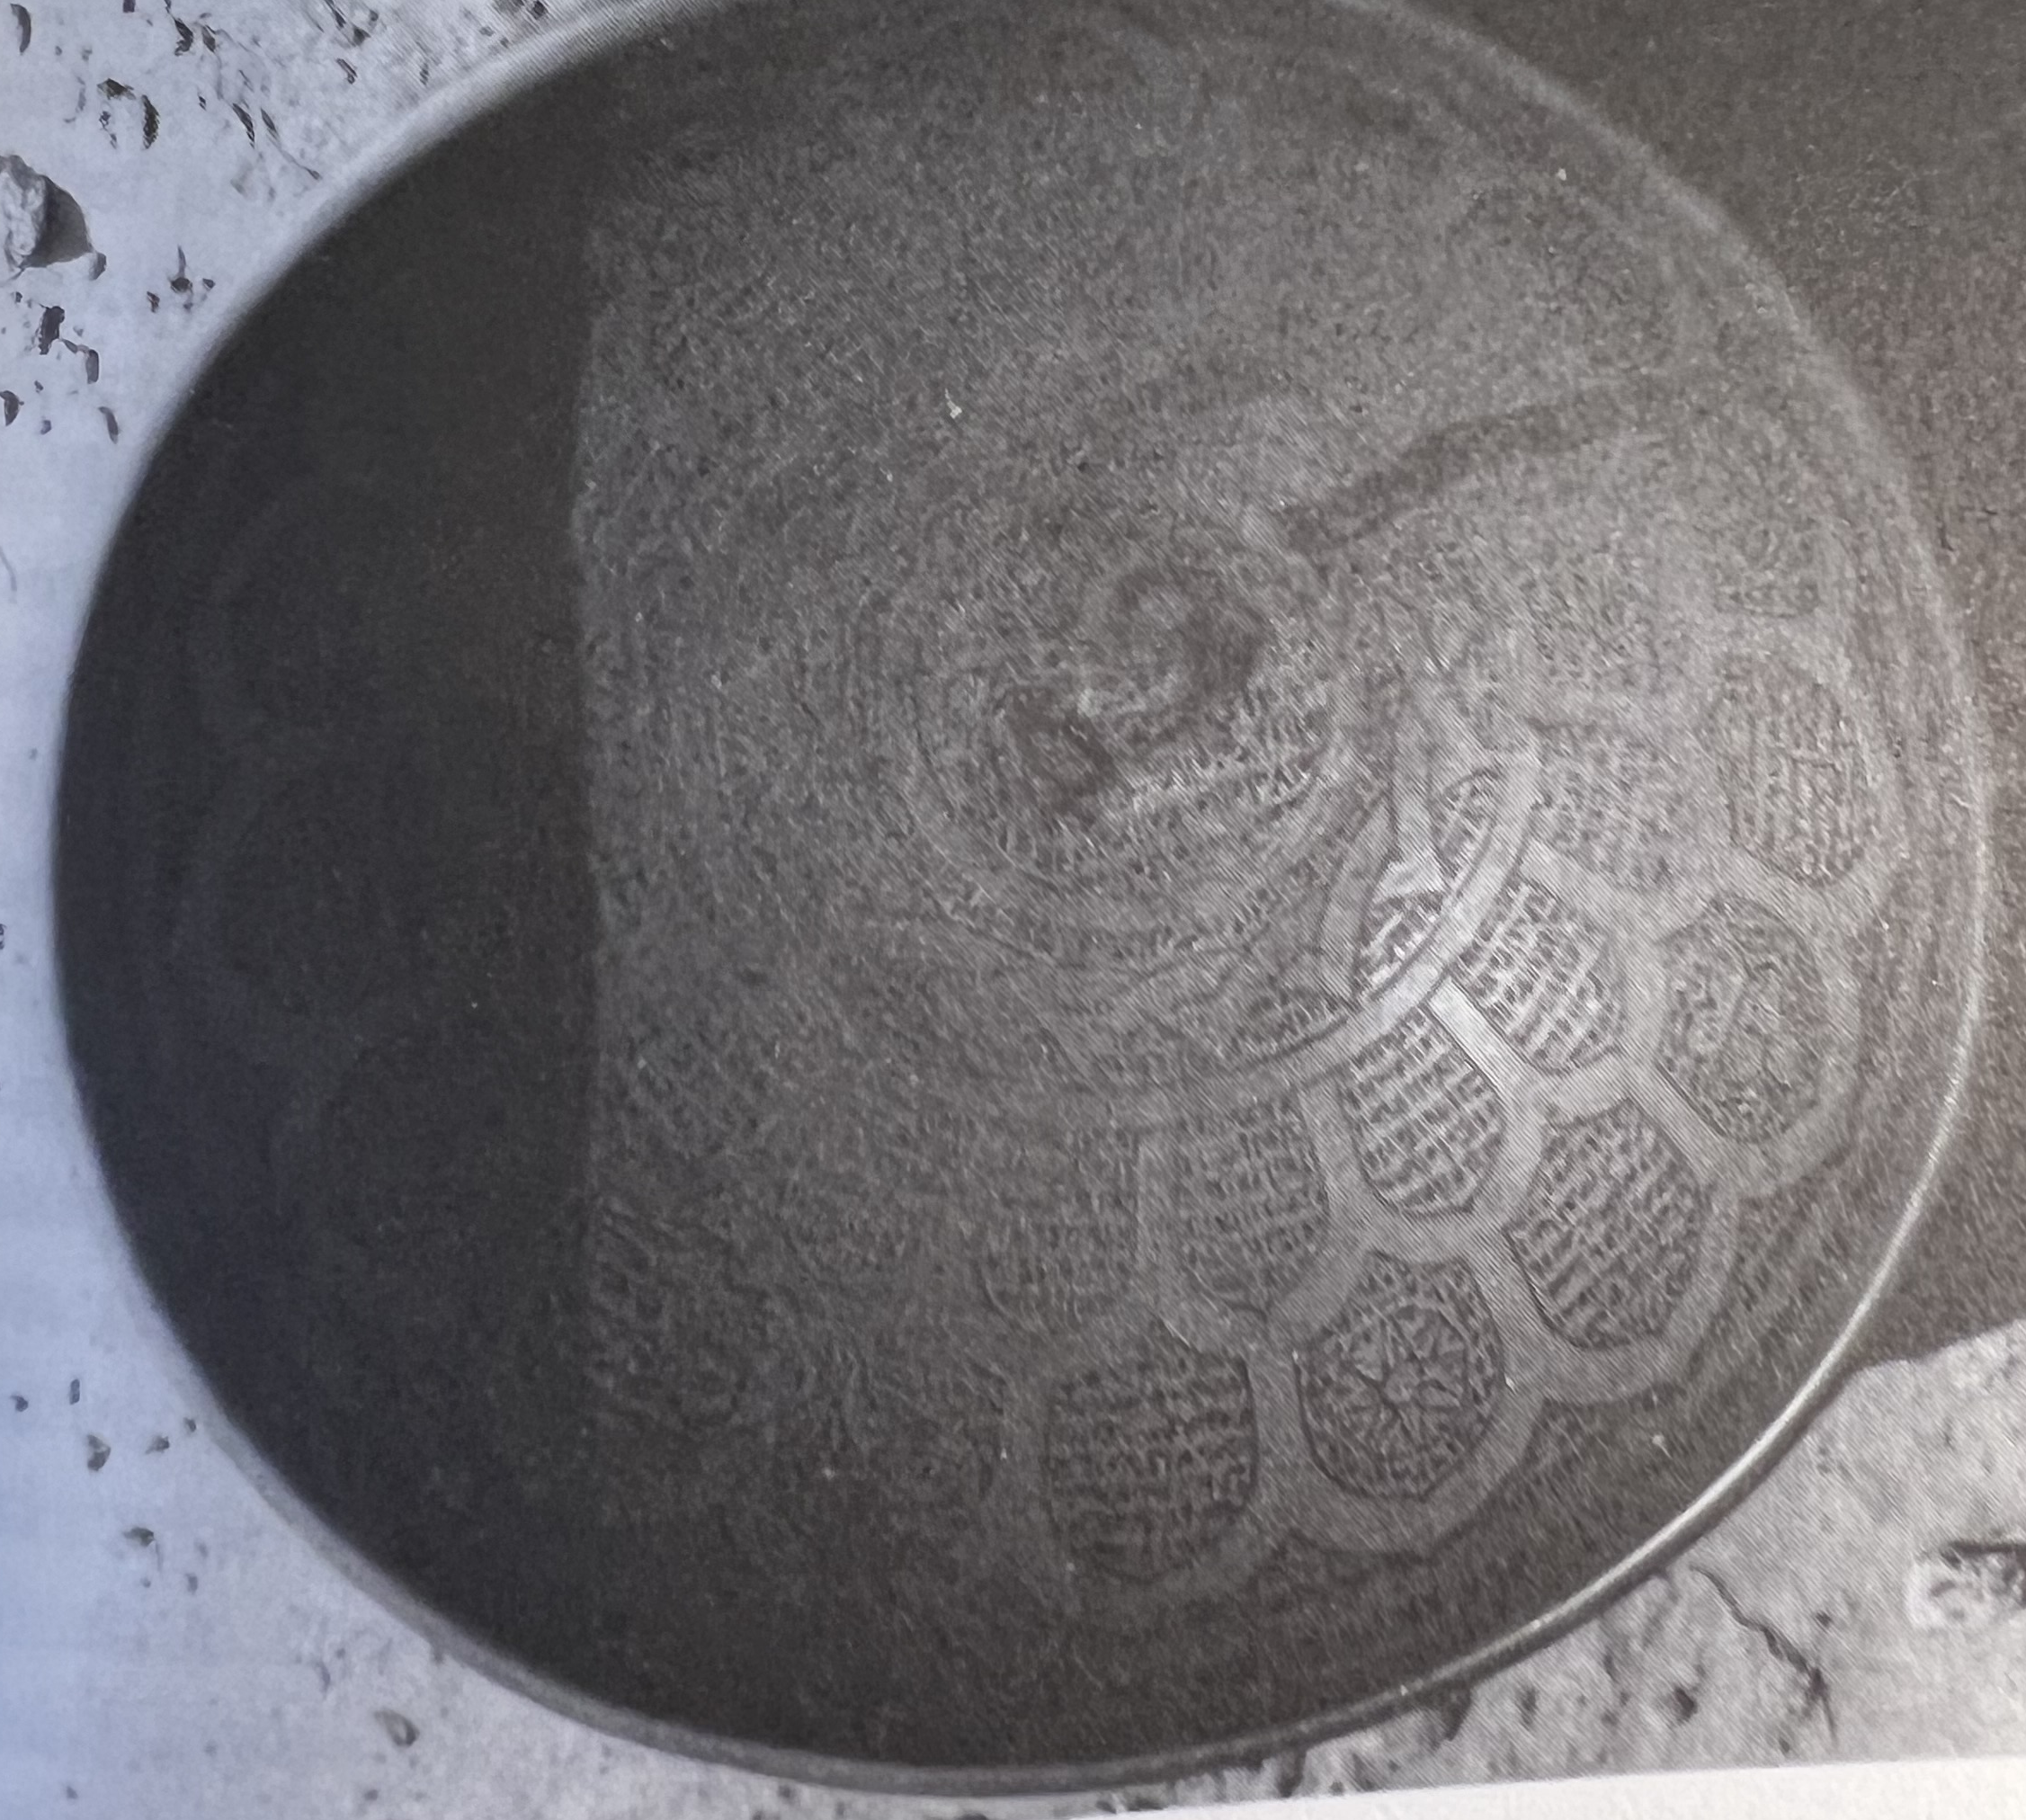
\includegraphics[width=0.8\textwidth]{HommeetIslam/Images/IMG_2457recadre.png}

 
    \label{fig:my_label}
\end{figure}

 \paragraph{3 registres concentriques}
L'ensemble du décor de la paroi intérieure se répartit sur trois registres, chacun délimité par un double cercle. On a ainsi trois doubles cercles concentriques dont le dernier suit les contours de la lèvre. 
Le premier registre, constitué par le fond de la coupe et délimité par un premier cercle concentrique, est occupé par un écrit de type magique qui reste à décrypter. On distingue autant que la détérioration et la réparation le permettent, des traits de hauteur inégale, des lettres de l'alphabet arabe. isolées, essentiellement \textit{hâ}', la (?), \textit{hâ} et \textit{kâf}, des chiffres, 6, 7, 95. Ils forment neuf lignes horizontales, la dixième suivant la courbure du cercle. Le second registre, situé dans la partie basse de la coupe, a essentiellement pour décor des bandes qui se chevauchent, formant seize pointes, une étoile à seize branches. L'espace résiduel est rempli d'écrits magiques, identiques aux précédents. Certains sont disposés sur le premier double cercle concentrique. Le troisième registre, enfin, occupe la plus grande surface de la coupe. Son décor est structuré par un motif de feuilles ou de pétales s'ouvrant en corolle, répartis sur deux hauteurs et décalés les uns par rapport aux autres. Ces « feuilles » forment autant de médaillons. La première série de médaillons, au nombre de seize, installée sur le second cercle concentrique, comprend exclusivement des écrits magiques identiques aux premiers, gravés sur six lignes, dont l'une est constituée par le second cercle concentrique. Quant à la série supérieure de seize médaillons, elle comporte, alternés, des représentations et des restes en arabe. 
\paragraph{un soleil, un chien, un scorpion, ...}On parvient à identifier les figures suivantes, dans le sens des aiguilles d'une montre : un soleil à huit rayons enfermé dans un cercle, un chien, un scorpion, un personnage (une femme avec un enfant, allaitant ?), un croissant de lune, un cheval, un serpent, un second personnage (personne mordue par un serpent ? ou possédée par un esprit malin ?). Autour d'eux, les mêmes écrits magiques, qui diffèrent cependant des précédents en ce qu'ils ne sont pas gravés sur des lignes.
L'ouvrage est fait de telle façon que la lune se trouve opposée au soleil, que l'un des personnages est dans l'axe de l'autre et les deux quadrupèdes face à face. En ce qui concerne les textes en arabe, il s'agit d'extraits du Coran, tous écrits sur huit lignes. En partant de la sourate liminaire, placée entre le chien et le scorpion, et en allant dans le sens des aiguilles d'une montre, on déchiffre :
\begin{enumerate}
   \item al-Fâtiha, jusqu'à
" .. ghayr al-maghdûb 'alayhim" ;
  \item précédée de la basmala,  une partie de s25v45 (« la Loi ou la
Salvation », al-Furqân), jusqu'à "la-jaalahu sâkinan", enchaînée à s6v13
(« Les troupeaux », al-An'âm), enfin quelques 4 mots non déchiffrés;
  \item la basmala, puis s84v1-4 (« La Déchirure », al-Inshiqâq), le verset
4 s'achève à : "wa algat má fiha", la fin reste à déchiffrer ;
  \item sans basmala, s24v35 (« La Lumière », al-Nür), jusqu'à « Júgad
min shajara mubâraka zaytâna là sharqiyya wa là [gharbiyya] », quelques lettres isolées (?), puis ra', les chiffres 7 et 2 ou 3
  \item la basmala, puis sur la 2° ligne, les 3 lettres liminaires apparaissant
au début de six sourates, celles de la Vache, d'al-'Imran, de l'Araignte, des Romains, de Lugmân et de la Prosternation (soit 2, 3, 29, 30, 31 er
32), à savoir \textit{alif}-lâm-mim, suivies de 3 mots non déchiffrés, puis sur la 3ème ligne, les 5 lettres liminaires de s19 (« Marie », Maryam), à savoir \textit{kâf}.
hã'-ya'-ayn-sâd, suivies de quelques mots non déchiffrés, puis sur la 4. ligne, les 3 lettres liminaires du début de s26 et   28 (« Les poètes » et « le
récit », al-Shu'ara' et al-Qasas), à savoir tâ'-sîn-mim, enfin les autres
lignes n'ont pu être déchiffrées ;
  \item la basmala, suivie de deux lignes et demi non déchiffrées, puis viennent peut-être une partie de s16v69 (« Les Abeilles », al-Nahl),
« yakhruj min butûni\textit{hâ} sharâb mukht\textit{alif} alwânuhu fihi shif@' » (?), et une partie de s17v82 (« Le Voyage nocturne », al-Isrâ'), « wa-nunazzil
min al-Our'ân mâ huwa shifà »" (?) ;
  \item la basmala (?), puis on lit \textit{hâ}-\textit{alif}, lâm-\textit{hâ}' al-rahmân al-rahim), suivi de s8v62-64 (« Le Butin », al-Anf@l) : le dernier mot du v63,
« hakîm », n'est pas très lisible et le v. 64 est déchiffrable jusqu'à « hasbuka Alla », quelques mots restent ensuite à comprendre;
  \item) sans basmala, 2v255 (« La Vache », al-Bagara, « verset du
Trône », ayat al-kursi), jusqu'à : « ... là yuhîtûn »'.
\end{enumerate}

L'espace compris entre les médaillons et l'ultime double cercle est
occupé par les écrits magiques déjà rencontrés plusieurs fois. Sur le cercle supérieur de ce dernier double cercle, enfin, est gravée une rangée
des mêmes écrits. Le décor de la paroi extérieure offre trois registres. Le premier est constitué par le fond de la coupe qui laisse deviner, en dépit de l'usure, le même type de composition magique que sur la paroi intérieure; la forme géométrique qui l'enserrait a disparu. On reconnaît ensuite un cercle concentrique constitué encore des écrits magiques. Le second registre occupe la partie médiane de la coupe. Les écrits magiques sont cette fois inscrits dans cinq cercles et cinq trapèzes alternés. Enfin, le troisième registre présente une ligne d'écriture qui suit le bord de la lèvre et s'étend sur tout le pourtour. Elle est gravée de telle sorte que le début du texte s'enchaîne sans rupture avec la fin. Cette phrase ininterrompue pourrait tenir dans un double cercle concentrique : le graveur s'est appliqué à ne jamais en dépasser les limites invisibles et à emplir l'espace de telle sorte qu'elle donne l'impression d'une bande circulaire continue, très décorative. Elle est chargée d'indiquer les vertus curatives de la coupe, comme c'est le cas pour la coupe A:
\begin{quote}
    « wa  li-mawlâna al-sultân al-Malik al-Mujähid al-muwakkal al-man.
sûr Abû al-Muzaffar Yasuf wa jumi a fiha manâfi mujarraba wa hiya li-
las'at al-hayya wa al-'agrab wa-li-al-hummâ wa al-mutlaga wa al-magh-
la wa li-al-kalb al-kalib wa li-al-maghass wa al-qawlanj wa al-shagiga
wa al-zarabân (?, sic) li-ibtâl al-sihr wa li-ramì al-dam wa li-al-ayn wa
al-nazra wa li-râd al-lawaga wa li-ifâdat al-masrû (?) wa li-usr al-baw!
wa li-sulh bayn al-aqrân (al-agrâb ?) wa li-nakad al-atfäl wa al- m.r: (?.
ou 'm.r.j?) bi\textit{hâ} al-mashür wa al-musâb wa al-bint (?) al-mu sira" ».
\end{quote}
Soit :
\begin{quote}
    {  « Pour notre Seigneur, le Sultan, al-Malik al-Mujähid, le manda-victorieux Abû al-Muzaffar Yûsuf26. Y [la coupe] sont réunis des bienfaits éprouvés par l'expérience, elle [sert] pour les piqûres de serpent et de scorpion, pour la fièvre, la parturiente? et augmenter le lait, pour les morsures de] chiens atteints de la rage, pour les douleurs stomacales et les coliques, la migraine et les élancements (?)?, pour conjurer les sortilèges, ou faire cesser le flux du sang, pour le mauvais œil et le mauvais sort  
pour empêcher la paralysie faciale et pour le rétablissement de la conscience des épileptiques (?), pour la dysurie, pour la réconciliation des adversaires (ou : les proches parents ?), pour les enfants agités. L'ensorcelé et celui qui est atteint, de même que la parturiente en difficulté (?), doivent [en boire le contenu par gorgées (?)].}
\end{quote}
\paragraph{Titulature de Saladin mais pseudo-épigraphique}
La titulature, la \textit{kunya} (= Abû al-Muzaffar) et le nom (ism = Yûsuf) \sn{à
moins qu'il ne s'agisse que d'une kunya = Abû al-Muzaffar Yüsuf}, mentionnés dans l'inscription, peuvent-ils servir à identifier le personnage ?

Et constituent-ils un élément fiable de datation de notre objet ? La même formule (sauf al-muwakkal) se retrouve chez Reinaud, sur les coupes n° 9420, chez Wiet, n° 14, chez Canaan - qui n'identifie pas - et surtout sur les deux coupes, dites de Saladin, étudiées par Zéki Pacha : \begin{quote}
     Izz li-mawlâna al-sultân al-malik al-mujâhid al-muayyid al-Mansûr Abû al-Muzaffar Yûsuf » et : « 'Izz. li-mawlânâ al-sultân al-malik al-mujâhid Abû al-Muzaffar Yasuf »
\end{quote} Les coupes dédiées à Saladin sont réputées nombreuses   mais ne sont pas nécessairement indicatrices d'un temps et d'un lieu de facture particulier. 
En effet, Wiet (1922, 319-28), dans un article très précis, critique la datation de Zéki Pacha en s'appuyant essentiellement sur des documents épigraphiques, mais aussi sur des chroniques : il montre que les inscriptions de ces deux coupes font entorse à la titulature de Saladin, et donc au protocole habituel, que ces formules sont rares au VI/XI s., et que les dates qui suivent la mention de souverains, sur les coupes, ne sont pas un gage de leur époque de fabrication; il concède toutefois que l'on puisse y voir une allusion au souverain ayyûbide - si l'on se rapporte à d'autres objets sur lesquels se trouve le même type d'anomalies - mais qu'en aucun cas, ces coupes ne peuvent être contemporaines de Saladin. Le style de la coupe B, de même que les conclusions de Wiet, font plutôt penser à une attribution posthume.
\begin{figure}
    \centering
       \sidecaption{Coupe B paroi externe}

  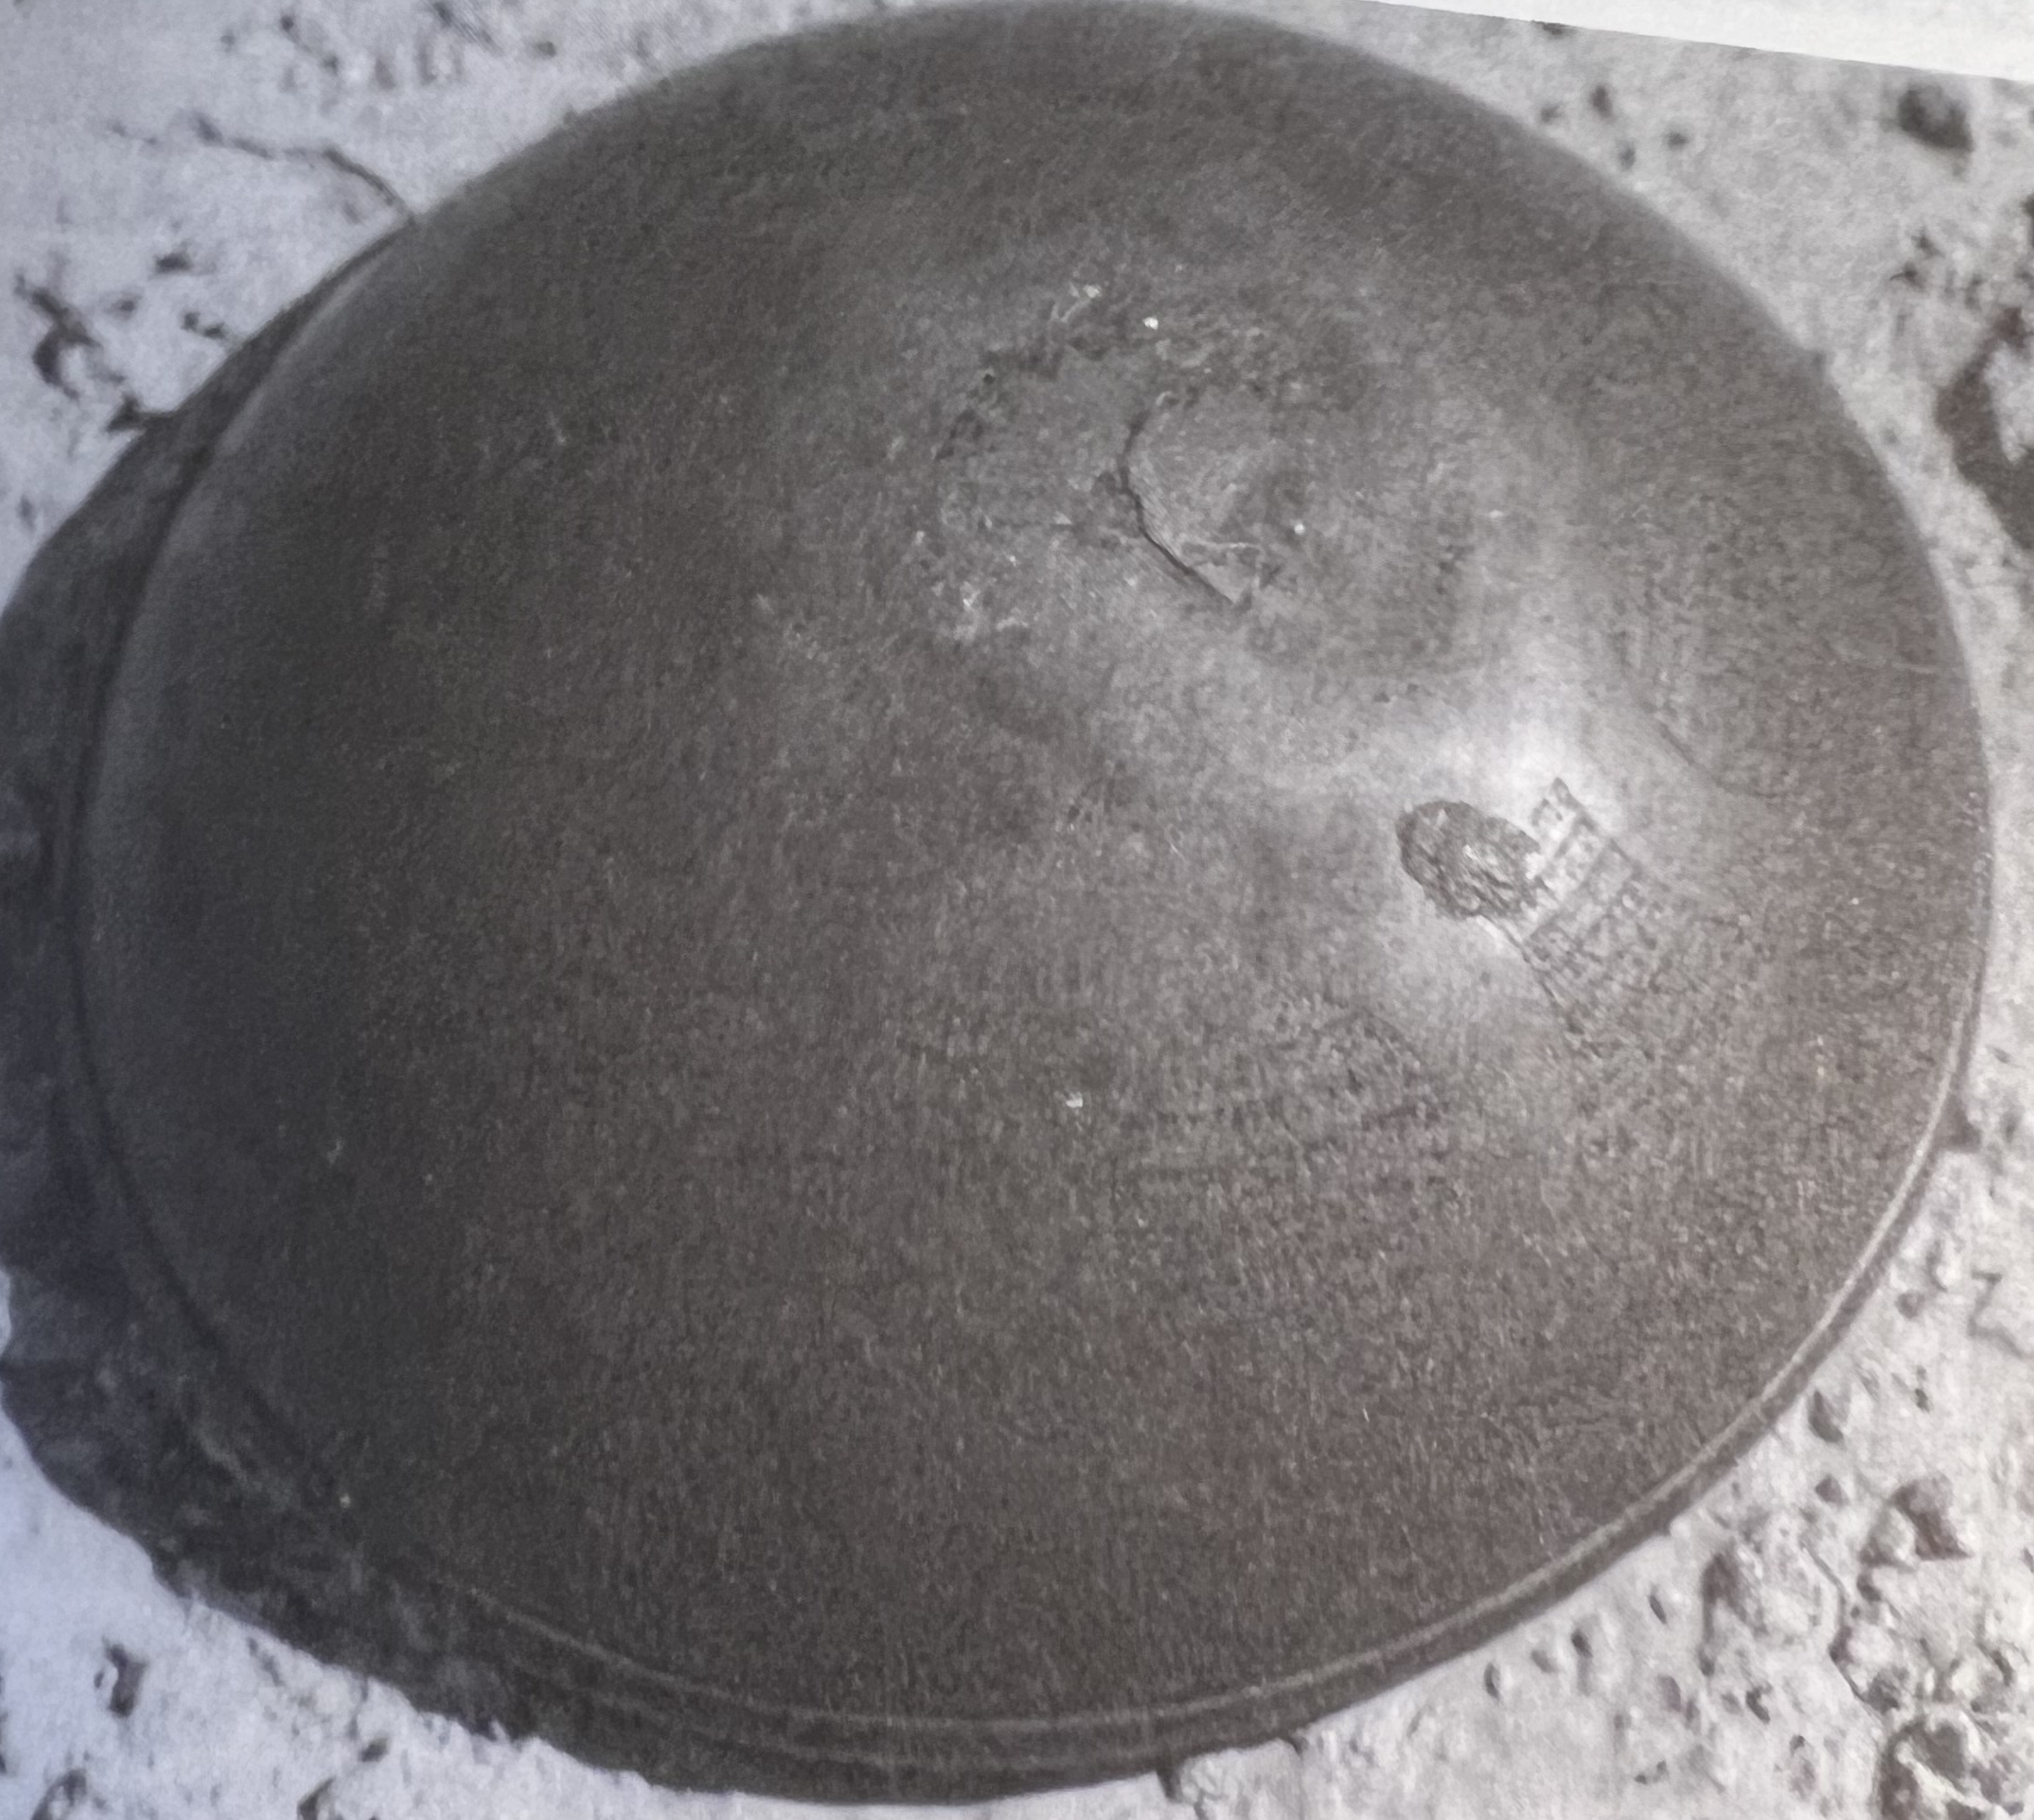
\includegraphics[width=\textwidth]{HommeetIslam/Images/IMG_2458recadre.png}

 
    \label{fig:my_label}
\end{figure}
  \paragraph{coupe anti poison}
L'étude des écrits, représentations, signes et figures géométriques des deux coupes fait apparaître un registre commun avec la talismanique. La symbolique de la coupe A, telle qu'elle se dégage à partir des éléments décrits, vient confirmer certaines de ses propriétés curatives. Tout d'abord, il s'agit d'une coupe anti-poison ; 

\paragraph{incantation valable pour toute oeuvre magique tenant compte de l'Evangile et de la Torah}al-Bânì cite une longue incantation (\textit{azima}) versifiée, valable pour toute œuvre magique : elle décrit les sept lettres spéciales, rappelle qu'elles sont le nom suprême de Dieu, puis que moyennant l'ajout de lettres de la Torah, des Evangiles et du Coran, l'on sera protégé des serpents, scorpions et lions?. Il s'agirait donc, dans l'ensemble, des animaux nuisibles ou devenus dangereux dont la coupe guérit de la morsure ou de la piqûre. En outre, elle aide en cas d'accouchement difficile, ce qu'indique la présence de la sourate \textit{al-
Inshiqâq}. 

\paragraph{coupe d'accouchement; analogie terre et accouchement  }
Des textes gravés sur d'autres coupes comparent le mouvement de la terre qui rejette ce qui est en elle et se vide, à celui de la femme qui met un enfant au monde dans des conditions favorables. Spontanément, les deux coupes m'ont d'ailleurs été présentées comme des « coupes pour l'accouchement », l'usage ayant probablement consacré cette fonction entre toutes. Selon al-Bûnî (s.d., (a), 91) encore, les trois bâtonnets, sans l'\textit{alif} sur le dessus, désigné simplement alors comme « protubérance » ou pointe de lance, et accompagnés du pentagramme, peuvent être employés pour guérir des maladies affectant l'intérieur du corps, dont les coliques (\textit{gawlanj}), auxquelles fait référence la liste des maux soignés par la coupe A. 
\paragraph{sceau de Salomon, sur les rouleaux Ethiopiens}
Enfin, les deux carrés entrecroisés gravés à l'intérieur de la coupe forment une étoile à 8 branches - cette étoile finissant dans un double cercle peut aussi représenter le soleil, dardant ses rayons? -. Décrite comme la gravure ou le diamant de l'anneau de Salomon, l'une de ses variantes se trouve sur les rouleaux magiques d'Ethiopie, où elle est appelée « sceau de Salomon »». Son centre, qui est également le centre de la paroi interne, est entièrement occupé de bâtonnets magiques. 
\paragraph{Pouvoir du roi Salomon - de son sceau}
Qu'il soit bague ou talisman, selon la Tradition, il donne à ce Roi son pouvoir sur les démons
-  pouvoir que le Coran lui reconnaît, dans la sourate Sâd, aux versets 34-39 - et donc sur la cause des maladies, ou tout au moins de certaines.
Dans certaines versions, il oblige les démons, qui sont des sortes de gardiens des maladies, à livrer les remèdes (Barkaï, 1996, 193). Dans l'ensemble, les démons - parfois appelés djinns - sont divisés en tribus liés à un habitat, et la maladie est ainsi territorialisée. Salomon n'éradique certes pas la maladie, mais, grâce à la puissance de son sceau, don du ciel, il est celui par lequel vient la guérison. On remarquera que le sceau de Salomon est gravé ici parmi les maux que la coupe est censée soigner.

\paragraph{Principe de guérison}
Leur liste étant incomplète, on ne fera qu'évoquer les maladies spécifiquement provoquées par les djinns ou les démons que Salomon et ses formules peuvent exorciser. Pour ce faire, on doit s'asperger ou se laver avec l'eau versée dans la coupe. L'architecture de la paroi interne est ici toute conçue et rythmée à partir de ce motif. Elle est largement construite selon le chiffre huit ou ses diviseurs. L'étoile à huit branches et les huit étoiles à six branches, structurant les parois interne et externe, indiquent singulièrement qu'elle en appelle à la protection de Salomon par qui vient la guérison, les autres grands pourvoyeurs de guérison étant Dieu et le Prophète (évoqué dans la formule gravée près de la lèvre supérieure de la coupe A).


La coupe B présente également l'image des animaux à piqûre et morsure (scorpion, serpent, chien, cheval) et le début de la \textit{sourate de la Déchirure}. L'un des deux personnages (femme avec un enfant, l'allaitant ?) rappelle son pouvoir de faire venir le lait. La \textit{basmala}, prononcée avant toute action et notamment avant d'ouvrir la bouche pour manger, de même que les Versets du Siège, appelés \textit{âyat al-hars wa l-hirz}, protègent contre les mauvais dinns ou démons. C'est le cas également des cercles.

\paragraph{sourate pour chaque maladie}
Thème que pourrait reprendre encore l'un des deux personnages (personne possédée par un esprit malin ?). Deux sourates renvoient aux sources de la guérison plutôt qu'elles ne visent une maladie en particulier. Le verset 69 de la sourate des \textit{Abeilles} fait en effet allusion aux pouvoirs curatifs du miel, qui fait partie des liquides versés dans les coupes, selon mon informateur, et à absorber donc par les malades. Les vertus du miel sont extrêmement nombreuses et constituent un thème de prédilection de la médecine prophétique. Par ailleurs, s17v82 (« Le Voyage nocturne ») rappelle le pouvoir curatif du Coran. D'une manière plus générale, s8v62-64 (« Le Butin ») martèle l'idée que : \textit{« Dieu te suffit »}. Quant à la sourate liminaire, ses vertus sont tellement innombrables, qu'elle n'est plus indicative : elle est bonne pour tout. Enfin, les deux Luminaires, le soleil et la lune, sont des symboles de vie, de prospérité et d'abondance, comme le remarque Canaan (1936, 100, 121). De la même manière que les deux Carrés entrecroisés contenant des écritures magiques, à l'intérieur de la
 coupe A, peuvent représenter le soleil sous la forme d'une étoile à huit pointes et qu'elle est structurée selon le chiffre huit, le soleil, dans la coupe B, compte également huit pointes. Par ailleurs, le fond de la coupe B est occupé par une étoile à seize branches, qui soutient sa composition interne en seize médaillons, puis en deux fois huit médaillons (à texte et à figures). Quelques coupes étudiées par ailleurs montrent une corrélation entre la présence des Luminaires et le chiffre 16 (cartouches ou cercles).
 \paragraph{Chiffre 8 et soleil}
Le rapport est donc net entre le chiffre huit et le soleil. On est tenté de mentionner alors le fait que huit correspond à la valeur isopséphique du \textit{hâ}, lui-même clé de la vie (hayât), selon un procédé bien connu en science des lettres. Cependant, les versets des sourates 6, 24 et 25, gravés sur la coupe B, rappellent l'omnipotence et l'omniscience de Dieu, cause de tout et à qui tout doit revenir, au-delà des deux Luminaires : 
\begin{quote}
   « C'est à lui qu'appartient ce qui subsiste dans la nuit et le jour »; « Dieu est la lumière des cieux et de la terre ».

\end{quote}
En guise de remarque finale sur les deux coupes, ne peut-on pas dire qu'elles contiennent ce qu'appartient ce qui subsiste dans la nuit et le jour ; \begin{quote}
    « Dieu est la lumière des cieux et de la terre ». 
\end{quote}
\paragraph{Cosmos}
En guise de remarque finale sur les deux coupes, ne peut-on pas dire qu'elles constituent une tentative de reproduire le monde clos du cosmos ?
\begin{figure}
    \centering
        \sidecaption{La Coupe comme représentation du cosmos. Coupe B paroi Interne et externe}
\includegraphics[width=\textwidth]{HommeetIslam/Images/IMG_2459recadre.png}

    \label{fig:my_label}
\end{figure}




En effet, le soleil qui préside à l'architecture interne des deux coupes, les cercles concentriques, les entrelacs de rubans ininterrompus, les textes eux-mêmes parfois écrits de telle manière qu'ils ne s'achèvent ni ne commencent, les motifs alternés qui se répondent, ainsi que la concavité et le caractère hémisphérique des deux objets (Canaan, 1936, 82), sans compter la composition organisée en registres, concourent à le reconstituer, quelques sourates rappelant que Dieu demeure le plus puissant, le plus savant et la Cause unique et suprême. Si l'on songe que le mode d'emploi des coupes consiste à passer par un liquide qu'on y verse, celui-ci se trouve donc en contact avec toute chose du monde : ambition holistique des coupes.
\paragraph{contexte Yemenite en cas d'accouchements et poisons}
Le recours aux coupes thérapeutiques est d'un usage bien établi au
Yémen, aussi bien dans la communauté juive que musulmane (Brauer, 1934, 182-3), surtout dans les cas d'accouchements difficiles ainsi que, concurremment à d'autres pratiques, contre le venin des serpents. L'acte de soigner différents venins, parmi lesquels celui des scorpions, est particulièrement investi par diverses médecines ou pratiques. C'est sans doute un indice de la fréquence du danger. 
\paragraph{fonctionnement des coupes : boire}
Selon l'un de ceux qui ont la responsabilité des coupes à la mosquée, leur mode d'emploi consiste principalement à boire le liquide - de l'eau, du bouillon - ou le miel que l'on y a versé. Le docteur Sarnelli rapporte, pour le Yémen des années 30, qu'il faut boire l'eau à petites gorgées en prononçant des louanges à l'endroit lu Seigneur des mondes, de ses anges et de ses prophètes. Pour les mêmes années, Brauer cite d'autres manières de les utiliser chez les juifs yéménites, il en sera question un peu plus loin (Brauer, 1934,182-3). Une véritable description ethnographique, susceptible de nous renseigner sur ensemble des étapes à suivre pour utiliser les coupes, manque cependant, que ce soit pour le Yémen, ou un autre lieu.
\paragraph{hypothèse : produit au contact des écrits communique au patient}
Le produit en contact avec l'ensemble des écrits et l'iconographie est chargé de communiquer quelque chose au malade, mais selon un principe qui reste à définir. Le liquide en relation avec les représentations des animaux nuisibles transmet-il au patient une partie de leur force, l'immunisant par assimilation de quelque chose de leur substance, agissant tel un contrepoison ? Ou au contraire, s'agit-il d'une mithridatisation\sn{Le fait de mithridatiser, d'immuniser en accoutumant à un poison.} ? Les présentations ont-elles une valeur prophylactique\sn{Qui prévient la maladie.
Mesures d'hygiène prophylactiques.}, comme c'est le cas sur des talismans chassant les bestioles et les chiens des maisons (Doutté.
194, 144-46) 
\paragraph{seéquence écrit liquide boire}
  La séquence écrits-liquide-boire, enfin, rappelle une pratique présente dans l'ensemble du monde arabe, qui consiste à écrire in papier, à l'encre noire ou de couleur, généralement des versets coraniques, et à le tremper dans un récipient empli d'eau, que l'on demande au malade de boire, notamment dans les cas d'ensorcellement!.

  \paragraph{bouillon, pratique aidant les paturientes, mélange de pratiques médicales}
Cependant, dans le contexte yéménite des hauts plateaux, il semble que le bouillon versé dans les coupes serve à soutenir plus spécialement les femmes en couches. Le bouillon de viande (\textit{marag}) est gras, robotif, et rassemble la substantifique moelle de la viande : il est offert en début de repas et particulièrement aux hôtes, comme un met prisé et recherché, le meilleur en somme. Il est par conséquent indiqué pour soutenir physiquement la femme en travail. Ici, le liquide n'est donc pas seulement conducteur ou à la rigueur stimulateur, dans l'économie de la guérison par les coupes, mais il apporte ses vertus propres, qui viennent en addition de celles des écrits et représentations. En médecine domestique, pour la même région du Yémen, le recours simultané à des médecines et à des médications différentes est courant. Plutôt que le reflet d'un tâtonnement thérapeutique, il faut y voir au contraire un discernement et la volonté \textit{d'attaquer le mal, dans son éventuelle pluralité}, dans toutes ses facettes. Les symptômes sont en effet soigneusement observés et triés, et, à partir d'eux, il s'agit d'évaluer les causes, qui peuvent être diverses pour un même symptôme. Symptômes et causes ne peuvent être tous traités de la même manière, et entraînent la décision de recourir à tel ou tel praticien. 
\paragraph{la maladie comme résultat de causes multiples}
En outre, lorsqu'il y a maladie, elle est toujours soupçonnée d'être le résultat de causes multiples, de nature diverse, déchaînées en même temps. L'utilisation des coupes, dans le cas qui vient d'être évoqué, n'est clairement pas un acte médical unique.
Des traînées de bougie apparaissent au fond de la coupe B. Sont-elles en rapport avec l'utilisation des coupes ? Enfin, on observera que la coupe B, réparée, est toujours considérée comme en service. Pourtant, les détériorations et les réparations ont entraîné, pour partie, la disparition du décor gravé au fond. 
\subsection{Institutionnalisation de pratiques magiques} \mn{\href{https://books.openedition.org/ifpo/1264?lang=fr}{le waqf} Deux catégories de waqfs selon la nature de la nue-propriété du bien :
\textsc{Waqf ṣaḥîḥ}. constitué de biens-fonds issus d’une propriété privée (\textsc{milk}) appartenant au fondateur lui-même et uniquement à lui-même. Ce waqf est une fondation ṣaḥîḥ, véritable et intégrale 
 
    \textsc{Waqf ghayr ṣaḥîḥ} composé des biens mîrî.   propriété d’État, lequel a sur eux tous droits d’exploitation et d’imposition. Tous ces droits sont exercés sous la tutelle du waqf. 


Le terme « \textsc{bīmāristān} », ou « māristān »,  désigne un établissement hospitalier pour les malades dont on espère la guérison.
}
 
 

\paragraph{un bien waqf depuis 1895}
Que ces objets soient \textit{waqf} et non \textit{milk} ne fait aucun doute pour leurs gardiens. On trouve d'ailleurs gravé sur la paroi externe de la coupe A, à la suite de la liste de ses propriétés, l'indication suivante: 
\begin{quote}
    « Wagafa al-
Hajj Husayn al-Hawâ (?) \textit{hâ}dhihi al-tâsa (sic) 'alâ al-Jâmi al-mahrûs
1313 » [legs pieux (\textit{waqf}) du Häjj Husayn al-Hawa (?) à la mosquée, la protégée, en 1313/1895-96]. 
\end{quote}
Outre l'intérêt immense d'avoir ici une date, certes tardive et à ne pas prendre pour une date de fabrication, on retiendra qu'un tel statut pour un tel objet est bien un fait. Et le cas qui nous occupe n'est peut-être pas singulier. 

\paragraph{les outils des hôpitaux sont \textit{waqf}} L'une des coupes signalées par
Ahmed Zéki Pacha, provenant du Bimâristân al-Mansär - du nom de son
fondateur al-Malik al-Mansûr Qalâwûn, en 683/1284, au Caire - et encore en service à la fin du XIX s., permet sans doute de ne pas limiter
au Yémen zavdite. L'ensemble des instruments utilisés à l'hôpital était en effet considéré comme \textit{waqf}. 
\paragraph{waqf oral sans enregistrement pour les objets}
Cependant l'établissement du statut juridique des objets qui nous occupent, pose problème.
Tout d'abord, ils ne seraient pas recensés par le registre des \textit{waqf}s. Il est difficile de croire à une négligence d'autant que leur qualité de bien \textit{waqf} n'est pas dissimulée. En 1998, dans une ambiance peu favorable il est vrais, la tentative de consulter ces registres du Ministère des \textit{waqf}-s a tourné court. Mais aux alentours de 1999, les objets semblent avoir été récupérés par ce même Ministère, selon ce qu'a révélé une nouvelle visite au lieu où ils étaient auparavant déposés. Jusque là, ils semblaient échapper au contrôle de l'administration des \textit{waqf}-s et à toute redevance.
Ils m'ont été présentés comme « \textit{waqf}-s oraux ». La procédure paraît connue et rodée. Le donateur vient et dit au récipiendaire : \begin{quote}
    « Je donne cet
objet en \textit{waqf} à la mosquée [awgaftu \textit{hâ}dha al-shay' alâ Jâmi kad\textit{hâ} ».
\end{quote} 
Et voilà tout. Elle est adoptée pour des objets isolés, tels les corans, les tapis, offerts à la mosquée par des particuliers, musulmans, et qui ne représentent ni de grosses quantités, ni sans doute une valeur à l'unité très importante : dans ce cas, le principe de l'absence de tout document fixant destinataires et frais de gestion (\textit{waqf}iyya), de même que l'absence de démarche d'enregistrement au Ministère des \textit{waqf}-s, sont admis et connus du même Ministères. Certains d'entre ces objets, tels les coupes, le Livre, ou tout ouvrage en général, peuvent porter - mais pas nécessairement - une inscription mentionnant qu'ils sont biens \textit{waqf}, d'autres non, tels les tapis. Il existe des tampons pour les ouvrages, usant de formules consacrées, où le donateur peut ajouter son nom. En somme le message est suffisamment clair : la mise en \textit{waqf} de ces objets signifie essentiellement qu'il est interdit à quiconque de les utiliser à des fins personnelles et de
 les vendre.
 \paragraph{prêté gratuitement. qui gère leur entretien ?}
Si les avoirs transmis sont clairement ici les objets, dans les faits, on ne voit pas bien en revanche comment se fait la prise en charge de leur entretien et, pour ceux qui nous concernent, des frais entraînés par l'accueil des demandeurs. En effet, ils suscitent des dépenses - même si on peut estimer qu'elles sont infimes - et pas de revenus. Nos quatre
objets sont prêtés sur simple demande, sans contrepartie d'argent, afin que même les plus démunis puissent se soigner. Autrement dit, ils génèrent plutôt du bien ou un service, du fait de leur usage thérapeutique (l-al-khayr). D'un autre côté, ils ont besoin d'être entretenus et réparés : les coupes se perforent par usure - c'est le cas de la coupe B, et il n'est pas rare de trouver des coupes dont le fond est percé - le manche du miroir a été soudé à la partie centrale et cette soudure peut se détériorer, enfin, la pierre risque d'être attaquée par le venin. 

\paragraph{tout le monde peut emprunter les coupes}Quant au destinataire, il s'agit de la mosquée, l'inscription de la coupe A le dit explicitement. Toute personne malade ou envoyée pour un malade et même si elle n'est pas du quartier ou de la Vieille ville, peut emprunter ces objets. Sur ce point, les dispositions légales ne font que reprendre un usage bien établi, en ce qui concerne les coupes tout au moins. Car même en propriété privée, elles ont toujours été prêtées à la demande et elles ne mentionnent dans leurs inscriptions aucun destinataire en particulier pour qui elles auraient été fabriquées, j'aurai à y revenir plus loin. De plus, l'usage collectif ancestral des coupes trouve parmi les catégories connues des fondations pieuses, sa case légale : il relève des fondations « d'orientation publique
ou charitable (\textit{waqf} khayrt) » (Deguilhem, 1995, 16) \mn{ si les bénéficiaires étaient désignés globalement, comme les pauvres en général, les mosquées, les madrasas, etc., le waqf était appelé \textit{khayrî}}.

Au regard encore de la définition d'une fondation pieuse, de son principe même, le cas qui nous occupe demeure problématique ou inédit, si tout \textit{waqf} fait normalement l'objet d'un écrit chargé de fixer les modalités par lesquelles des revenus seront alloués à un (ou plusieurs) destinataire(s) (Deguilhem, id, 15). En ce qui concerne des dispositions particulières, force est de constater que le Yémen a fait l'objet de peu d'études, aussi bien en langue arabe qu'en langue européenne, sur les diverses modalités de fondations pieuses y ayant cours; il reste donc relativement méconnu sur ce point.
\paragraph{tradition orale}
Il est encore possible de se reporter à la transmission orale, si l'on veut tenter de préciser la provenance et la date à laquelle ces objets ont acquis leur statut. En se plaçant du strict point de vue de la collecte des données, les informations restent imprécises et contradictoires, liées aux souvenirs de chacun et à l'ancienneté de leur présence dans ces lieux. Sur les quatre objets concernés, l'un était propriété du  actuel : c'est lui qui l'a donnée en \textit{waqf} à la mosquée. D'après ce dernier, les trois autres objets bénéficient du même statut depuis très longtemps, puisque non seulement il les a toujours vus, mais ils sont là depuis plusieurs générations, si l'on se fie au témoignage de son grand-père. Tandis que son fils déclare que la \mn{p. 332}
coupe A n'est devenue \textit{waqf} de la mosquée que depuis six ans [données de 1995 : elle était auparavant la propriété d'un membre de la famille, habitant hors de Sanaa, sans pourtant qu'il puisse préciser où (la mention de bien waqf, gravée sur la coupe A, n'indique pas plus de lieu). Au terme de la discussion, une solution est finalement proposée, qui intègre les divers épisodes. Elle consiste à dire que la coupe a été volée par les tribus entrées dans Sanaa lors de l'assassinat de l'Imam Yahyâ, en 1948  ; puis qu'elle a été restituée, sans autre détail sur les péripéties. Il est vrai que ces coupes magiques sont considérées comme des objets précieux (\textit{tuhfa}).
Finalement, les désaccords entre les informateurs ne portent à aucun moment sur le statut légal des objets. L'information substantielle à retirer d'un point de vue ethnologique concerne, semble-t-il, la perception reçue des hommes de tribu, chez les citadins : selon eux, ce sont des pilleurs, susceptibles de s'emparer de biens \textit{waqf}-s et, au total, ils représentent des responsables idéals, pour ne pas dire miraculeux.

Au total, ces quatre objets sont des biens donnés par des particuliers
en \textit{waqf} khayri à une mosquée, sans \textit{waqf}iyya, i. e. d'acte fixant en particulier par écrit leur gestion, dans le cadre des modalités de répartition des revenus; ils n'apparaissent pas non plus dans les registres du Ministère des \textit{waqf}-s. On peut cependant se demander si ce statut légal avéré ne représente pas par ailleurs une « solution » intéressante étant données le relations conflictuelles entre ce Ministère et ses administrés, et si elle n'est pas une modalité de la résistance, par ex., à une mainmise sur les fondations pieuses, sans même supposer de position idéologique. De plus la coupe A a un itinéraire compliqué, dont la traçabilité ne semble par toujours claire, et n'est « sauvée » de ses lacunes que par des solution pour le moins providentielles. Quoi qu'il en soit, l'inscription gravée su la paroi externe de la coupe A atteste que la mise en \textit{waqf} de ce type d'objet est séculaire. Son statut juridique est de la sorte officialisé, rend public. Depuis plusieurs générations, aucun interdit majeur ne pèse donc sur la pratique qui consiste à rendre un tel bien fondation pieuse et à rattacher à une mosquée. \textbf{C'est pourquoi, on parlera ici d'institutionnalisation d'une pratique magique.}

\subsection{Transmission du savoir et efficacité }

\paragraph{le responsable de la mosquée}
La responsabilité de la « gestion » des quatre objets magiques, en tant que biens \textit{waqf}s, dépend du système régissant la succession à la charge suprême, dans la mosquée concernée. C'est, en l'occurrence, aux représentants de la même famille qu'échoit le titre de \textit{Mudir al-Jami} depuis des générations. 
\paragraph{possession sans pouvoir magique}
Hériter de cette responsabilité n'est à aucun moment lié au fait de posséder un savoir en magie. Cela laisse planer la possibilité d'un divorce entre le responsable, ses références, ses convictions personnelles d'une part, et la nature des objets, son devoir de les prêter, d'autre part.
C'est précisément le cas à propos d'un autre objet déposé en \textit{waqf} : l'un de ses « gardiens » doute de ses vertus magiques, même si cela n'engage pas nécessairement son opinion sur les coupes. Ses critiques sont formulées d'un point de vue rationnel. Le mode d'emploi des coupes semble de plus largement connu??, D'autre part, le statut de \textit{waqf} khayri de ces deux coupes impose un usage non privé et non personnel. La manière d'utiliser les objets qui nous occupent est-elle alors ou non représentative d'une pratique ou d'une tradition et en définitive sur quoi repose l'efficacité des coupes ?
\paragraph{des objets d'abord nobles}
Si l'on se rapporte aux travaux antérieurs sur les coupes, il apparaît qu'elles sont la propriété de particuliers ou de familles dont rien n'indique un rapport particulier avec les pratiques magico-thérapeutiques. Regardées aussi comme des objets précieux, elles appartiennent au mobilier d'illustres familles et, à ce titre encore, elles figurent dans les Musées : certaines \sn{p. 334}
sont des pièces d'orfèvrerie, fabriquées à partir de matériaux nobles, et leurs vertus leur confèrent en outre de la valeur. 

\paragraph{demandé par le malade et non le praticien, pas nécessaire}
Elles sont habituellement prêtées à ceux qui les réclament - en principe le malade ou une personne dépêchée par lui, et non un praticien - sur leur simple demandes. En effet, le mode d'emploi ne semble pas nécessiter la présence d'un praticien. Lorsqu'il est gravé et indique les maux soignés par la coupe, seuls le liquide à y verser et la manière de l'utiliser (boire à petites gorgées, asperger, etc.) sont spécifiés (Canaan, 1936,125-26). En outre, à défaut cependant de véritable étude ethnographique, les rares relevés ne mentionnent pas davantage l'existence de praticiens. 

\paragraph{Rôle de  l'accoucheuse}Néanmoins, l'étude ethnologique d'Erich Brauer sur les juifs yéménites, qui a l'avantage de donner une chaîne un peu plus complète d'opérations, mentionne le rôle de l'accoucheuse : la femme aidant à l'accouchement (\textit{mahjeräh}) emprunte une coupe, qui a déjà donné de bons résultats, aux riches familles connues pour en posséder une ; elle la pose alors sur le ventre de la parturiente pour faciliter l'accouchement. S'y ajoute, le cas d'une praticienne juive yéménite qui exerce au Nord du Yémen et que je n'ai pu observer.
En dehors de ces exemples notables, on ne relève en général pas d'intervention d'un intermédiaire reconnu pour ses compétences en magie ou, en tout cas, pour soigner avec ce type d'objet.qu'elles ne sont pas réservées à un utilisateur particulier - de même que dans notre cas de \textit{waqf} khayr? - et, sauf exception, elles ne mentionnent aucun nom de propriétaire ou de destinataire pour lequel elles auraient été spécialement fabriquées, Sur ce point, elles se distinguent des coupes araméennes et de certains bols arabes en poterie, employés dans les années 30, qui portent le nom du malade et celui de sa mère, suivant des pratiques talismaniques encore très répandues en monde arabe et subsaharien (Canaan, 1936, 80, 123-4). Le rapprochement avec les talismans qui sont imprimés et vendus dans des boutiques en monde arabo-musulman, tel le fameux \textit{Salr 'uhûd Sulaymân}, est tentant, mais une fois utilisés par son acheteur, peuvent-ils être empruntés par tout autre ? Les deux coupes, objet de cette étude, sont donc représentatives dans l'ensemble, car d'un usage collectif qui ne suppose, à aucun stade de leur emploi, le concours d'un homme de magie.
\paragraph{d'où vient la magie ?}
L'efficacité des coupes reposerait-elle alors sur leur fabrication par un homme de magie ? Quelques travaux des années 20 et 30 en font une spécialité de Persans, dont les ateliers auraient été soit en Perse, soit à La Mecque". Annette Ittig, s'appuyant sur le fait que le nom du destinataire-propriétaire n'est pas spécifié sur les coupes, avance qu'elles peuvent être fabriquées par des ateliers ayant une forte productivité, et l'existence de copies médiocres vont dans le sens de cette observation (Ittig, 1982, 94 ;
Canaan, 1936, 117). 
\paragraph{référence astrale ?}
Mais 19 des coupes déjà publiées se réferent à un événement astral sous les auspices duquel elles auraient été gravées, 13 donnent à la suite une (pseudo ?)-date de fabrication, et sur ces 13, 8 sont « datées » du VI- XIIs.
On sait déjà que la date de l'une de ces coupes est problématique, car supposée être gravée lorsque la lune était en Scorpion, en l'année
570/1174-75, pour \textit{al-Mansûr Asad al-Din Shirkuh}, l'oncle de Saladin : or, Shirkuh est mort en 564 H. Enfin, l'événement astral est parfois évoqué par des formules quasiment identiques. A-t-on affaire à un phénomène historiquement situé, qui consistait à vouloir placer l'efficacité des coupes sous le signe ou l'influence d'un événement astral, sans vraiment en maîtriser la connaissance ? Il est clair, en tous les cas, que l'on a affaire pour partie à des copies, même si - c'est très important de le souligner
- aucune des coupes publiées n'est identique, de même qu'aucune de celles que j'ai vues. Les artisans apparaissent donc comme chevronnés, car capables d'introduire des variations tout au moins dans l'architecture du décor, et certains ont eu éventuellement des compétences en talismanique; on songe moins à des praticiens de la magie auxquels aurait été confié le soin de graver. 
\paragraph{des artisans avec des compétences variables}
L'étendue de leur savoir (religion, astrologie, magie,.) et de leur technique peut être exceptionnel, mais certains imitent les motifs, en particulier magiques, sans plus en avoir la clé. Cela signifie que même dans le cas où les inscriptions des coupes aiguillent sur l'existence d'hommes de magie au moment de leur fabrication, cela n'est pas toujours le cas. Enfin, dans l'hypothèse où les formules se référant à un événement astral auraient été copiées, doit-on penser qu'il s'agit simplement de faux ? Ne faut-il pas plutôt considérer que l'artisan procédait ainsi parce que la simple évocation de l'événement astral, doublée parfois du nom d'un souverain, ou rapporté à l'époque de Saladin, venant en addition des écrits et motifs gravés sur la coupe, ajoutait à la valeur et à l'efficacité de la coupe (Savage-Smith, 1997, 73) ? 
\paragraph{une copie, même pouvoir que l'original}
Certains textes gravés sur les coupes, ne laissent aucun doute sur le fait qu'être une copie, représente une valeur ajoutée. D'après Canaan, les Palestiniens expliquent ainsi l'origine des coupes : les bons anges en employaient de semblables pour faire leurs ablutions. Ils en oublièrent un jour quelques exemplaires à côté de la source où ils avaient l'habitude de se rassembler pour se laver. Un homme passant par là les trouva et s'en empara. Les propriétés miraculeuses de la coupe furent bientôt découvertes. Des copies en furent réalisées, qui manifestèrent les mêmes propriétés (Canaan, 1923,130;
1936. 127) D'après Canaan, les Palestiniens expliquent
ainsi l'origine des coupes : les bons anges en employaient de semblables
pour faire leurs ablutions. Ils en oublièrent un jour quelques exemplaires
à côté de la source où ils avaient 1'habitude de se rassembler pour se
laver. Un homme passant par là les trouva et s'en empara. Les propriétés
miraculeuses de la coupe furent bientôt découvertes. Des copies en furent
réalisées, qui manifestèrent les mêmes propriétés (Canaan, 1923,130;
1936, 127)16.  
 Comme au premier jour, selon ce récit, la coupe abandonnée puis reproduite conserve son pouvoir.

 \paragraph{pouvoir du bronze et cuivre jaune}
Il viendrait alors principalement des écritures et figures gravées qui le communiquent au malade par le biais d'un liquide absorbé, aspergé, la surface la plus investie par cet ensemble de signes restant l'intérieur des coupes". Il faudrait également compter avec les propriétés des différents métaux utilisés, généralement le bronze et le cuivre jaune. Mais si le liquide versé varie en fonction du mal, il ajoute ses propres vertus à l'opération et l'eau elle-même possède ses propriétés particulières" : à preuve, la recherche d'une eau « plus active ». Canaan mentionne que le en fin d'operation
souvent par l'indication que les coupes sont éprouvées (« \textit{hâ}dhihi al-tasa mujarraba »), plus rarement par une « garantie » de qualité, en tant que copies, sans doute d'originaux réputés. Certaines coupes sont reconnues nettement plus efficaces que d'autres, telle celle dédiée à Salâh al Din (Zéki Pacha, 1916,254), ou comme Brauer l'a relevé. La répétition d'une formule ou la multiplication d'un même type de sentence, des versets par exemple, voire l'ancienneté des coupes y contribue. 
\paragraph{un pouvoir décuplé par la Mosquée}
Pour finir, la présence de ces objets dans la mosquée leur confère certainement un pouvoir supplémentaire auprès des utilisateurs. Cette remarque va, du reste, dans le sens de certaines inscriptions figurant sur les coupes, qui soulignent qu'elles ont été produites à La Mecque ou pendant le mois de Ramadân.
\begin{Synthesis}
    En résumé, les coupes sont généralement utilisées sans qu'œuvre un homme de magie ou quelqu'un qui, à des degrés divers, aurait des notions de magie. Elles sont d'usage collectif, elles ne sont en principe pas fabriquées pour un destinataire en particulier. De ce point de vue, les deux coupes, objet de notre étude, peuvent donc être ramenées au cas général.
Quant à la fabrication des coupes en général, nous savons encore fort peu sur leurs artisans. Cependant même dans les cas où les inscriptions sur les coupes évoquent le recours à une astro-magie, il peut s'agir de la simple référence à un événement astral, sans rapport certain avec le moment de leur fabrication. On ne peut en induire d'emblée que l'artisan a effectivement eu des notions de magie ou d'astrologie. L'efficacité des coupes guérisseuses serait donc intrinsèque en ce sens qu'elle ne supposerait pas nécessairement le concours d'un homme de magie.
\end{Synthesis}

\section{Du magico-thérapeutique}
Le rapprochement entre les écrits, représentations, signes, et figures géométriques apparaissant sur les parois des coupes et les talismans a \mn{p 339}
déjà été fait, non seulement par des études, mais il est aussi bien attesté par l'inscription suivante gravée sur certaines coupes : « Hadhihi al-tilas-mât etc. ». L'expression, au pluriel, semble bien désigner en effet ce qui est gravé sur leurs parois.
À notre connaissance cependant, aucune dénomination vernaculaire ne désigne les coupes elles-mêmes comme talisman. D'autre part, les spécificités que l'on vient de dégager, à savoir que les coupes ne font intervenir, généralement, aucun praticien dans leur mode d'utilisation, qu'elles ne sont pas fabriquées pour un destinataire nominalement désigné, qui en aurait besoin pour résoudre un problème précis et pour son usage particulier, et enfin, que l'on constate largement un phénomène de copies, et de copies de copies, tout ceci en ferait une catégorie très particulière de talismans. Rappelons, au sujet du dernier point, l'analyse très éclairante que fait Constant Hamès à propos de l'usage talismanique du Coran : 
\begin{quote}
    il y a pratique talismanique à partir du moment où un homme de l'art œuvre en re-travaillant le « matériel » coranique (Hamès, 2001, 95).
\end{quote}
Enfin, reste le problème de l'apport du liquide dans l'usage des coupes. A ce titre, l'exemple yéménite est particulièrement intéressant et clair, car il s'inscrit dans le cadre d'une médecine domestique qui « attaque le mal » par addition des thérapies. C'est pourquoi, la dénomination de « coupes magico-thérapeutiques » a paru préférable. 
Les deux coupes étudiées ici appartiennent à la collection de biens de fondation pieuse (\textit{waqf}) d'une mosquée yéménite ; l'une d'entre elle porte, gravée sur sa paroi externe, sa date de mise en \textit{waqf}, en 1313/1895.
L'étude des écrits, représentations et figures géométriques des deux coupes fait largement apparaître un registre commun avec la talismanique. Le motif du soleil, central, structure leur architecture interne. Ne faut-il pas voir dans le décor des coupes l'ambition de représenter le monde clos du cosmos, aux destinées duquel préside Dieu, le seul à pouvoir réellement guérir, le Suffisant ? Leur mode d'emploi consiste à verser un liquide (ou du miel) qui est absorbé par le malade (ou son envoyé).
\paragraph{Contexte yéménite}
Une véritable étude ethnographique manque cependant, pour le Yémen, mais même à titre comparatif. Les coupes sont particulièrement utilisées au Yémen pour faciliter l'accouchement. Le bouillon de viande que l'on verse pour ce faire, illustre le fait que le liquide n'est pas seulement conducteur ou à la rigueur stimulateur, dans l'économie de la guérison par les coupes, mais qu'il apporte ses qualités propres, en addition de celles des écrits et représentations. En médecine domestique, sur les hauts plateaux yéménites, le recours simultané à des médecines et à des médications différentes est courant. Ces objets sont présentés comme \textit{waqf}s oraux, statut a priori paradoxal. Néanmoins, leur statut juridique de biens \textit{waqf}-s d'une mosquée, permet de dire qu'il y a ici institutionnalisation d'une pratique magique, d'une part. D'autre part, qu'ils relèvent des fondations « d'orientation publique ou charitable » (\textit{waqf} khayri). Ce statut fait qu'elles sont prêtées à toute personne qui les demande à condition bien sûr que ce soit pour un malade. Il a aussi pour conséquence que le mode de transmission de la responsabilité de ces objets est lié aux \textit{règles de succession à la charge de l'intendance de la mosquée, et n'a donc pas de rapport avec une quelconque compétence en magie}. 
\paragraph{Une tradition dans l'utilisation ?}
La question se pose alors de savoir si le mode d'emploi des deux coupes, tel que transmis par la mosquée, s'inscrit dans une tradition, en est le reflet. A terme, on se demande sur quoi repose leur efficacité. Sur la base des études déjà nombreuses sur ces objets, il est possible d'avancer prudemment que l'usage des coupes est généralement collectif, qu'elles ne sont pas fabriquées au nom d'un bénéficiaire particulier, qu'aucun praticien de la magie, enfin, n'intervient dans leur mode d'emploi. Les deux coupes du Yémen entrent alors dans le cas général. En outre, si nous ne disposons encore que de peu d'informations sur leur fabrication et leurs artisans, les événements astraux sous l'égide desquels les coupes sont réputées avoir été fabriquées, comme en font état des inscriptions sur la paroi de certaines d'entre elles, même s'ils suggèrent le recours à une astro-magie, ne laissent pas une totale certitude sur le rapport réel entre la référence à cet événement astral et leur fabrication. Un mythe d'origine des coupes, relevé par Canaan, véhicule l'idée que la copie peut avoir autant d'effet que l'original. 
\paragraph{Efficacité intrinsèque}
L'efficacité des coupes guérisseuses serait donc intrinsèque en ce sens qu'elle ne supposerait pas nécessairement le concours d'un homme de magie: elle reposerait essentiellement sur les écrits, représentations et figures géométriques gravées sur leurs parois. \textbf{Le lien déjà établi entre ces éléments gravés et les talismans est pertinent, mais il est prudent, à notre avis, de désigner les coupes comme magico-thérapeutiques, plutôt que comme talismaniques, sous peine de passer sous silence le rôle important du liquide qui doit y être versé.}

\section{Bibliographie}
\begin{itemize}
    \item 

BARKAI, Ron, 1996, « Médecine, astrologie et magie », in A l'ombre d'Avicenne. La médecine au temps des c\textit{alif}es, Institut du Monde
Arabe/Snoeck-Ducaju \& Zoon, 1996, 189-193.
BEY, Dr Ahmed Issa, 1928, Histoire des Bimaristans (Höpitaux) à l'époque islamique. Discours prononcé au Congrès Médical tenu au Caire à l'occasion du centenaire de l'Ecole de médecine et de
l'Hôpital Kasr-el-Aîni, Le Caire, imp. Paul Bamey, 116 p.
AL-BÜN1, Ahmed ben Ali, (a), s. d., Shams al-madrif al-kubra.
Beyrouth, al-Maktaba al-thaqâfiyya, 576 p.
\item (b). s. d., Manbo usúl al-hikma, Beyrouth, al-Maktaba al-haditha
li-al-tibâa wa-al-nashr, 335 p.
AL-DAYRABI, s. d., Mujarrabát al-Dayrabi al-kabir, al-musamma bi-
fath al-malik al-mujid al-mu' allaf li-naf al-abid wa-bi-\textit{hâ}mishiha al-
shaykh Abi Abd Alläh Muhammad b. Yüsuf al-Sanúsi al-Hasani
Beyrouth, Sanaa, al-Maktaba al-haditha, Maktabat al-Sanhani, 160 p.
DEGUILHEM, Randi, 1995, Le \textit{waqf} dans l'espace islamique. Outil de pouvoir socio-politique, Damas, IFD, 337 + 100 p.
DOUTTÉ, Edmond, 1994, Magie et religion dans l'Afrique du Nord, Paris, J. Maisonneuve et P. Geuthner, 1994 (Ire éd. 1908), 617 p.
DOZY, R., 1881, Supplément aux dictionnaires arabes, Leyden, E. J.
Brill, 1881,2 t.
DUGAT, Gustave, 1853, « Etudes sur le traité de médecine d'Abou
Djäfar Ah'mad, intitulé : Zad al-Moçafir 'La provision du voya-geur' », Journal Asiatique, I, 288-253.
DUNLOP, D. M., 1960, « Bimâristân », E.1.2, Leyden-Paris, E. J. Brill.
G.-P. Maisonneuve, 1259-1262.
EL-BOK\textit{hâ}RI, 1984, Les traditions islamiques, trad. et notes par O.
Houdas, Paris, A. Maisonneuve, t. 4.
ÉTIENNE, Marc, 2000, Heka. Magie et envoûtement dans l'Egypte ancienne, Paris, Réunion des musées nationaux, « Les dossiers du musée du Louvre », 126 p.
HAMES, Constant, 2001, « L'usage talismanique du Coran », Revue de l'histoire des religions 218, 1, « Les usages du Livre saint dans l'islam et le christianisme », 83-95.
JANSEN, J. J. G., 1996, "al-Shawkâni", E.J.2, Leiden, E. J. Brill, 390.
LANE, E. W., 1877, Arabic-English Lexicon, Londres, William and
Norgate, 2 t.
MERCIER, Jacques, 1979, Rouleaux magiques éthiopiens, Seuil, 37 p. +
40 tab.
MERMIER, Franck, 1988, Les souks de Sanaa et la société citadine (République Arabe du Yémen), thèse de doctorat de l'EHESS (dir.
Gilbert Grandguillaume), 2 tomes, 573 p.
PORTER, Venetia, 1987, "The Art of the Rasulids", in Werner Daum (ed.), Yemen. 3000 Years of Art and Civilisation in Arabia Felix, Innsbruck, Frankfurt/am/Main, 232-253.
PSEUDO-MAJRITI, 1933, Das Ziel des Weisen. 1. Arabischer Text, her-
ausgegeben von Hellmut Ritter, Leipzig, B. G. Teubner, "Studien der
Bibliothek Warburg", VI + 416 p.
RITTER / PLESSNER, 1962, Das Ziel des Weisen von Pseudo-Majriti,
translated into german from the arabic by Hellmut Ritter and Martin
Plessner, London, The Warburg Institute/Univ. of London, LXXVIII
+ 435 р.
SERJEANT aLsAA L Ons les c{alif}es, Paris, Snoeck-Ducaiu \& 7 on cerne. la medecine au
" temps des c\textit{alif}es, Paris, Snoeck-Ducaju \& Zoon/Institut du Monde Arabe.
ANSALDI, Cesare, 1933, Il Yemen nella storia e nella leggenda, Rome.
ARTS D'ORIENT, juin 1999, Catalogue Paris-Drouot Montaigne de la vente du lundi 7 juin, pièces 111à 113, 38.
BRAUER, Erich, 1934, Ethnologie der jemenitischen Juden, Heidelberg,
XIX + 402 p. + 8 tableaux.
CANAAN, Tewfik, 1914, Aberglaube und Volksmedizin im Lande der
Bibel, Hamburg, L. Friederichsen \& co, XI+ 153+6 tables.
\item 1923, "fiâsit er-radifeh (Fear Cup)", Journal of the Palestine Oriental Society [JPOS] 3, 122-131.
\item 1936, "Arabic Magic Bowls", JPOS 16, 79-127.
\item 1937, "The Decipherment of Arabic Talismans", Berytus 4, 69-110,
\item 1938, "The Decipherment of Arabic Talismans", Berytus 5, 1938,
141-151.
CANOVA, Giovanni, 1995a, "Nota su una coppa magica egiziana", in :
Azhàr. Studi arabo-islamici in memoria di Umberto Rizzitano (1913-
1980), a cura di A. Pellitteri e G. Montaina, Palermo, 59-68.
\item 1995b, « La tâsat al-ism : note su alcune coppe magiche yemenite », Quaderni di Studi Arabi 13, « Divination, magie, pouvoirs au
Yémen », 73-92.
CASANOVA, M., 1891, « Notice sur une coupe arabe », Journal asia-tique VIII, 17, 323-330.
\item 1921, « Alphabets magiques arabes », Journal Asiatique XI, 18,
37-55, et 1922, XI, 19, 250-262.
CINGOLANI, Cinzia, 1987-88, Coppe magiche del museo Gayer-Anderson del Cairo, tesi di laurea, Università di Venezia, (Je n'ai pu consulter ce travail).
DAVIS, S., 1955, "Divining Bowls, Their Uses and Origin: Some African Examples and Parallels from the Ancient World", Man 55
(143), 132-5.
FODOR, Alexandre, 1990, "Amulets from the Islamic World", Catalogue of the Exhibition held in Budapest in 1988, The Arabist, Budapest studies in arabic 2, Budapest, 160 sq.
GRASSI, Vincenza, 1987, "Una 'coppa magica' proveniente dall'Egitto",
Studi magrebini XIX, 65-89, 7 pl.
ISMAIL, Muhd, 1922-23, "Two Arabic Medecine-Cups", Journal of the
Bombav P
f the Royal Asiatic Society (JBBRASI XXVI, n° 2.
ologiques
alicmanic Bowl". AnD344
KRISS. Rudolf / KRISS-HEINRICH, Hubert, 1962, Volksglaube im
Bereich des Islam II : Amulette, Zauberformein und Beschwörungen, Wiesbaden, Otto Harrassowitz, 126-137, pl. 100 à 111.
LANE, Edward William, 1923 (?). The Manners and Customs of the
Modern Egyptians, London/Toronto, E. P. Dutton, (réimp.).
XXV+630, 255, 261.
NASSAR, Nahla, 2001, « Notice de la coupe magique au nom de Nûr al-
Din Mahmud ibn Zangì » in : L'Orient de Saladin. L'art des Ayyoubides, Paris, IMA/Gallimard, n° 211, 223.
OMAN, Giovanni, 1981, « Le 'coppe magiche' nella medicina popolare
araba », in : La Bisaccia dello Sheikh. Omaggio ad Alessandro
Bausani islamista nel sessantesimo compleanno, Quaderni del semi-
nario di iranistica, uralo-altaistica e caucasologia dell'Universita'
degli sudi di Venezia 19, 215-219.
\item 1987, « Materiali per lo studio delle coppe magiche nella medicina
popolare araba », Quaderni Ticinesi [di) Numismatica e Antichita classiche 16, 337-358.
"REGOURD, Anne, 2002, « Une coupe thérapeutique du Yémen »,
L'aventure des écritures (CDRom), Paris, BNF, RMN.
\item 2005, « Une coupe magico-thérapeutique au Louvre (inv. MAO
1284) », in Livres de Parole. Torah, Bible, Coran, Catalogue de l'exposition, Paris, B.N.F., 187-9 + illustr.
REHATSEK, E., 1874, Description de deux coupes dans Indian
Antiquary III, 36.
\item 1875a, "Explanations and Facsimiles of eight Arabic Talismanic
Medecine-Cups", Journal of the Bombay Branch of the Royal Asiatic Society [JBBRAS] X(1871-74), 150-162.
\item 1875b, « The Evil Eye, Amulets, Recipes, Exorcisation, \&... », JBBRAS X(1871-74), 299-315.
\item 1880, « Magic », JBBRAS XIV (1878-1880), 199-218.
REICH, S., 1937-38, « Quatre coupes magiques », Bulletin d'Etudes
Orientales 7-8, 159-175, pl. XI-XII.
REINAUD, J. T., 1828, Monumen[t)s arabes, persans et turcs, du Cabinet de M. le Duc de Blacas et d'autres cabinets (ou : Descriptions des monuments musulmans du cabinet de M. le Duc de Blacas), II, Paris.
ROSU, Arion, 1992, « Une coupe magique d'époque moghole au musée
Guimet », Journal asiatique CCLXXX, 3-4, 251-277.
SARNELLI, Tommaso, 1934, « Notizie preliminari sui risultati della mia
missione sanitaria nell'alto Yemen : con particolare riguardo alla
medicina indigena », Archivio italiano di scienze mediche e coloniale
15, 1-43.
SAVAGE-SMITH. Emilie. 1997  
 
Mopping the Universe, The Nasser D. Khal F Colection of Islamie
Ma, vol. XII, London and Oxford The tour Foundation, in associa-
Ain with Azimuth Ed, and Oxford Univers Press 72-99;
SPOER, H., Henri, 1935, "Arabic Magie Medicinal Bowls", Journal of
African and Oriental Society [JAOS] 55, 237-256.
1938, "Arabic Magic Bowls II : an astrological Bowl", JAOS.
58,366-383.
VON GLADISS, Almut, 1999, "Medizinische Schalen. Ein islamisches
Heilverfahren und seine mittelalterlichen Hilfsmittel", Damaszener
Mitteilungen 11, 147-161, pl. 22 à 25.
\item 2001, « Notice de la coupe magique Syrie ? 621H/1224 », in : L'Orient de Saladin. L'art des Ayyoubides, Paris, IMA/Gallimard, n° 211,224.
WALKER, John, 1934, Folk Medecine in Modern Egypt, London, Luzac, 128 p. + 2 pl.
WIET, Gaston, 1932, Catalogue général du Musée arabe du Caire.
Objets en cuivre, Le Caire, IFAO, 77-78, n° 3213 (pl. LXIII) ; 94,
n° 3862 (pl. LXI) ; 95, n° 3897 (pl. LXIII) ; 95-96, n° 3906 (pl. LXII) ;
100, n° 3965 ; 101, n° 3981 ; 121, n° 4431 (pl. LX) ; 150, n° 9364 ;
150-51, n° 9380 ; 151, n° 9420 ; 265-69, n° 530 à 544 ; 286, index « coupe magique ».
\item 1958, « Inscriptions mobilières de l'Egypte musulmane », Journal Asiatique 246, 237-285, pl. 8.
\item et alii, 1937-1954, Répertoire chronologique d'épigraphie arabe, Le Caire, IFAO, 1937, VIII, n° 2952 ; 1937, IX, n° 3319, 3389, 3392-
3394 ; 1939, X, n° 3648; 1944, XIII, n° 5043-5045 : 1954, XIV, n° 5247,5262, 5455.
WÜNSCHE, Michela, 1993, « Traditionelle Heilmethoden im Jemen »,
Jemen Report, 24/2, 31-2
YA \textit{kâf}I, YA SHÄFI, 1999, The Tawfik Canaan Collection of Palestinian
Amulets. An exhibition, October 30, 1998-February 25, Birzeit University, 50 p.
ZEKI PACHA, Ahmed, 1916, « Coupe magique dédiée à Salah ad-Din (Saladin). Titres royaux, tolérance et portrait de Salâh ad-Din », Bulletin de l'Institut Egyptien X, Sè série, 241-289. « Note additionnelle sur une seconde coupe de Salah ad-Din », en fin d'article.
ZWEMER, Samuel, M., 1920, The influence of animism on Islam. An account of popular superstitions, New York, MacMillan, VIII+246
p. + 1 pl. (coupe).
\end{itemize}
 

  \part{Mission : de l'histoire à la théologie}
 
\chapter{Introduction}

\mn{Catherine Marin / Xavier Gué}

Vers une théologie chrétienne de l'Islam : était le thème des précédents séminaires.
Maintenant, de l'histoire à la théologie.
Partir des textes du magistère, et faire un travail inductif sur la théologie sous-jacente.
\begin{Synthesis}
Quelle est notre pratique missionnaire aujourd'hui ?
\end{Synthesis}

Un séminaire, c'est un travail universitaire, si tout le monde participe.

\section{Pourquoi il faut repenser la catégorie de mission ? Entre crise et résurgente}

\subsection{des crises}

Pendant des siècles, 
\begin{quote}
Le cadre théorique était simple : Mt 28, 18-20, "allez et faites des disciples". 
\end{quote}

Bosch : 
\begin{itemize}
\item propagation de la foi
\item Emergence du royaume de Dieu
\item nouveaux croyants
\item nouvelles Eglises
\end{itemize}

\begin{Def}[mission]
\textit{missio } : Dieu envoie.

\end{Def}
Peu à peu, c'est l'Eglise qui envoie. Telle une conquete. Cette conception est entrée en crise au XX sous des coups internes et externes : 
\begin{quote}
depuis la fin de Vatican II, on assiste à de tels changements... qu'il est difficile d'imaginer une stabilité de l'article
82 - article \textit{théologie de la Mission} dans \textit{catholicisme}
\end{quote}

\paragraph{les facteurs de la crise} 
\subparagraph{la décolonisation} la mission comprise comme \textit{domination}. L'idée de richesse à la source de la colonisation se transforme en \textit{civilisation} et donc on apporte aussi la religion, partie de la civilisation Européenne.

\paragraph{Vatican II}
\begin{quote}
On peut être sauvé sans être baptisé, par l'esprit saint, être associé à la mort et resurrection du Christ d'une certaine manière.
GS 65
\end{quote}

Les missionnaires apportaient le salut (FX sauvant les âmes). 

\subparagraph{l'esprit saint précède la mission}

\subparagraph{Notra Aetate} Respect des autres Traditions religieuses. Aucune référence au magistère. \textit{inattendu.}

\begin{Synthesis}
Le christianisme était pensé comme universel, c'est à dire adapté à toutes les cultures.
supériorité du Christianisme prouvé par son succès (autoréférence ?).
\end{Synthesis}
\NA change la vision. Fin de l'optimisme où le monde deviendrait chrétien. 

\subparagraph{On passe de la figure du missionnaire à l'Eglise mission} Ad Gentes  : l'origine de l'Eglise est missionnaire car le Christ est missionnaire. 

\paragraph{le décret \textit{Ad Gentes}} \href{https://www.vatican.va/archive/hist_councils/ii_vatican_council/documents/vat-ii\_decree\_19651207\_ad-gentes\_fr.html}{Ad Gentes}, Un texte de compromis, avec des tensions internes. Demande des pères de lier organiquement le décret des missionnaires à \LG. Texte publié en 1965. Tendance à spécialiser les missions aux pays de mission. Alors que d'autres voulaient aussi inclure l'évangélisation aux défavorisés.



\section{Un certain retour missionnaire}

\subsection{La nouvelle Evangélisation} 
Sous l'impulsion de Paul VI et Jean-Paul II, avec deux évènements : la création du Conseil Pontifical pour la Nouvelle Evangélisation, en 2012, et le synode sur la nouvelle Evangélisation.

\paragraph{Nouvelle Evangélisation} Le terme Évangélisation est récent dans l'Eglise, d'abord utilisé pour désigner les Luthériens. L'Eglise préférait le terme de \textit{mission}. Le concile Vatican I n'emploie qu'une seule fois évangélisation. Alors que Vatican II l'utilise régulièrement.

\paragraph{Exhortation dans le monde moderne - 1975} 
\begin{quote}
En effet, \ldots des temps nouveaux d'évangélisation.
\end{quote}

A Nova Uta, Jean-Paul II : la nouvelle croix de bois, levée... En ces temps nouveaux, l'évangile est de nouveau annoncé. La nouveauté vient de la nouveauté des Temps.
\textit{Redemptoris Mission} les pays de tradition chrétienne ont perdu des chrétiens vivants avec la sécularisation. Card. Suard, 1947 : Évangélisation nécessaire dans le monde ouvrier.


\subparagraph{François abandonne le terme Evangélisation pour Mission} dans \textit{Evangelii Gaudium}

\begin{quote}
\textsc{III. La nouvelle évangélisation pour la transmission de la foi}

14. À l’écoute de l’Esprit, qui nous aide à reconnaître, communautairement, les signes des temps, du 7 au 28 octobre 2012, a été célébrée la XIIIème Assemblée générale ordinaire du Synode des Évêques sur le thème La nouvelle évangélisation pour la transmission de la foi chrétienne. On y a rappelé que la nouvelle évangélisation appelle chacun et se réalise fondamentalement dans trois domaines.[10] 
\begin{itemize}
\item En premier lieu, mentionnons le domaine de la pastorale ordinaire, « animée par le feu de l’Esprit, pour embraser les cœurs des fidèles qui fréquentent régulièrement la Communauté et qui se rassemblent le jour du Seigneur pour se nourrir de sa Parole et du Pain de la vie éternelle ».
 [11] Il faut aussi inclure dans ce domaine les fidèles qui conservent une foi catholique intense et sincère, en l’exprimant de diverses manières, bien qu’ils ne participent pas fréquemment au culte. Cette pastorale s’oriente vers la croissance des croyants, de telle sorte qu’ils répondent toujours mieux et par toute leur vie à l’amour de Dieu. 
\item  En second lieu, rappelons le domaine des « personnes baptisées qui pourtant ne vivent pas les exigences du baptême »,[12] qui n’ont pas une appartenance du cœur à l’Église et ne font plus l’expérience de la consolation de la foi. L’Église, en mère toujours attentive, s’engage pour qu’elles vivent une conversion qui leur restitue la joie de la foi et le désir de s’engager avec l’Évangile.

\item  Enfin, remarquons que l’évangélisation est essentiellement liée à la proclamation de l’Évangile à ceux qui ne connaissent pas Jésus Christ ou l’ont toujours refusé. Beaucoup d’entre eux cherchent Dieu secrètement, poussés par la nostalgie de son visage, même dans les pays d’ancienne tradition chrétienne. Tous ont le droit de recevoir l’Évangile. Les chrétiens ont le devoir de l’annoncer sans exclure personne, non pas comme quelqu’un qui impose un nouveau devoir, mais bien comme quelqu’un qui partage une joie, qui indique un bel horizon, qui offre un banquet désirable. \textit{L’Église ne grandit pas par prosélytisme mais « par attraction ».}[13]
\end{itemize}

\end{quote}
\begin{Synthesis}
Toute Eglise est missionnaire. Pour François, nous sommes \textit{disciple missionnaire} car c'est intrinsèque.
\end{Synthesis}
\mn{Travailler le thème de disciple missionnaire en Cvx ? influence Jésuite ? Matteo Ricci ? Question}

\paragraph{L'Evangélisation de Rue} sous l'influence des milieux anglo saxons, on va aborder l'évangélisation directe, avec une approche marketing\mn{cf le Congrès Mission : technique marketing au service de l'annonce. Mais quelle théologie ?}.

\paragraph{Conclusion} Regarder l'approche historique pour mieux comprendre théologiquement ce qui est en jeu.

David Bosch. p19. 

\section{L'approche de la prédication}

\subsection{Histoire}
Adapte la mission à la situation économique : les moines n'utilisaient pas le terme de mission. Saint Martin de Tours a évangélisé parce que c'était normal \mn{paysan et paien même racine}.


\paragraph{Comment passe-t-on du profane au sacré} {La vallée des Saints : Sacralisation} du passage du profane au sacré. 

\paragraph{Professionnalisation de la \textit{mission} avec les jésuites}  au XVI. 
Lettres de François-Xavier. On passe d'un baptême d'abord en Inde au passage, au Japon, par le préalable de la compréhension de la culture.

\paragraph{Colonisation} Les Eglises issues de la colonisation se sont appropriées le christianisme avec leur caractère propre. Cf Eglise du Vietnam.


\paragraph{Va et vient historique}
Dans le temps, on va s'inspirer du passé pour réfléchir à la manière d'être missionnaire. Par exemple, les \textit{réductions} jésuites en Amérique du Sud. Les Chrétiens prenaient en charge l'aspect religieux et sociale et économie. Ces réductions se sont inspirées des moines. Avec le village autour des moines : va et vient tout simple autour d'un monastère \textit{pour la plus grande gloire de Dieu}.

Le Cardinal  lavigerie : \textit{"il faut faire comme les moines du XIX" }: équilibre de vie : coeur spirituel, social et économique. 

\mn{
Deux mille ans d'évangélisation et de diffusion du christianisme Broché – Illustré, 20 janvier 2022
de Jean Comby (Auteur), Claude Prudhomme (Auteur)}

\section{Indications méthodologiques}

\paragraph{Sources}
\paragraph{Mise en récit} cf Ricoeur : trois phases 
\begin{itemize}
\item j'ai découvert des choses
\item je mets en ordre la vie d'un missionnaire
\item récit en lui-même, récit partiel car on n'a qu'une vision partielle de ce qui s'est passée.
\end{itemize}

\begin{Ex}
Surin : 10 ans sans publier. ne pas extrapoler.
\end{Ex} 

\begin{Def}[Story / History]
En Français, on n'a que histoire.
\end{Def}

Il y a ce qui est écrit et ce qui n'est pas écrit. Par exemple, on sait qu'il s'est passé quelque chose d'important près du lieu de mission. le missionnaire n'en parle pas. pourquoi ?

\paragraph{Historicité d'un fait}
Tout être humain porte une histoire. Il faut toujours être vigilant sur notre analyse de l'histoire. On ne peut pas juger de ce qui s'est passé il y a trois cents ans. Michel de Certeau : \textit{l'écart}. Il faut éviter le jugement car on fait le court circuit du \textsc{contexte}, politique, historique, spirituel.

\begin{Ex}
Missionnaires au XIXeme, marqué par l'outrage de la Révolution et la nécessaire \textit{réparation}. Les missionnaires sont beaucoup plus rigides au XIX qu'au XVII / XVIII. 
\end{Ex} 


\paragraph{Témoignage}
\begin{quote}
18 Jésus s’approcha d’eux et leur adressa ces paroles : « Tout pouvoir m’a été donné au ciel et sur la terre.
19 Allez ! De toutes les nations faites des disciples : baptisez-les au nom du Père, et du Fils, et du Saint-Esprit,
20 apprenez-leur à observer tout ce que je vous ai commandé. Et moi, je suis avec vous tous les jours jusqu’à la fin du monde. » Mt 28
\end{quote}

\paragraph{Annonce} lié au témoignage : individuel mais communautaire. Des congrégations religieuses. La communauté où est né le missionnaire. 

Henri René Marrou
\begin{quote}
le Christianisme ne crée pas les civilisations; il les sauve
\end{quote}
Et de fait, des grammaires de 30 langues africaines; arts.  


\subsection{Que va-t-on englober dans l'histoire des missions ?}

\paragraph{Une professionalisation depuis le XVI}

\paragraph{Mais battue en brèche par les femmes et les acteurs locaux}

\paragraph{Histoire de l'envoi / histoire de la réception} Il y a aussi le pouvoir local : si un Roi local ne veut pas de missionnaires, il n'y aura pas de missionnaires. cf un Roi en Guinée. 

\paragraph{Histoire du christiansime}

\paragraph{retour entre le témoignage des missionnaires revient sur les vieilles terres chrétiennes} On se nourrit dans ces vieilles terres.

Marrou : écrire l'histoire, sortir de soi. Prise de conscience de l'écart : ne pas juger ce qui était par rapport à ce qui était. On fait de l'histoire pour mieux comprendre le présent.
\begin{quote}
Christianisme comme histoire; pédagogie 
Danielou
\end{quote}

\section{A lire}

Hugues Didier - Correspondance de François Xavier , 1532 -1552, Desclée de Brouwer. 


 \chapter{Les modèles de mission dans le Nouveau Testament}

\mn{Dynamique de la mission Chrétienne David Bosch 20/9/22}

\begin{Synthesis}
Concile de Jérusalem : pas une concession, une position commune pour \textit{préserver l'unité}.
\end{Synthesis}

\begin{quote}
 Selon cette dernière opinion, le fait que la rencontre ait
eu lieu à Jérusalem et que les apôtres y aient joué un rôle crucial, a été
accepté de bonne grâce par Paul et la délégation d'Antioche. Ceux-ci
n'ont pas fait simplement un geste de conciliation. La position de
Jérusalem et des apôtres correspondait à une identité commune (cf.
Holmberg 1978: 26-28). La« concession» n'a pas été exploitée par
les «colonnes» de Jérusalem: tout comme Paul, ils redoutaient la
division et étaient prêts à tout pour sauvegarder l'unité: Le désir e
s'écouter était mutuel. Les chefs de Jérusalem ne voulaient nen faire
qui mette en péril les communautés chrétiennes non juives, dont
plusieurs existaient déjà depuis plus de dix ans (Hengel 1986: 116).
Ils étaient capables de distinguer entre la piété de la Torah et le coeur
de la vie chrétienne. Tous ces facteurs ont préparé la voie à l'entente
dans ce concile, que Meyer (1986: 1oi) caractérise comme étant « la
décision politique capitale de l'Église du I°'  siècle». . . .
Bien entendu, avant et après le concile, les hebrawi chrétiens
restèrent obstinément critiques à l'idée d'une mission indépendante de
la Torah (Meyer 1986 : 99). Au concile, ils formaient une minorité.
Mais dans les années qui suivirent, ils gagnèrent toujous pus
d'influence dans l'Église de Jérusalem. Le récit de Luc sur la s1tuat1on
conflictuelle qui prévalait lors de la dernière visite de Paul à Jérusalem
(Act 21: 17-26) semble bien le confirmer (Hengel 1986: 116s).
Les divergences à propos des conclusions du concile persistèrent
jusqu'à la Guerre juive. Il est vrai que, avant même la destruction du
temple et la chute de Jérusalem, la plupart des chrétiens juifs avaient
quitté la Judée. Au moment où la guerre éclata, le mouvement des
sadducéens était déjà en perte de vitesse. Avec la destruction du
temple, les sadducéens perdirent leur dernier appui. Les remous de la
guerre précipitèrent leur fin, mais aussi celle des zélotes et des
esséniens en tant d'organisations séparées. Seuls les pharisiens
survécurent à la crise, en partie grâce à leur enracinement dans les
synagogues, dispersées à travers le pays juif et au loin. Aussitôt après
la guerre, ils arrivèrent à établir leur autorité, pratiquement sur tout le
judaïsme. Dès qu'ils eurent le dessus, Ils introduisirent des restrictions
pour les chrétiens juifs qui étaient encore membres e synagogues
locales. Il devint toujours plus difficile de rester pratiquant Juif et
même temps que chrétien. Autour de 85 ap. J.-C., cela devint
impossible. Les \textit{Dix-Huit Bénédictions}\sn{La 12ème bénédiction : Pour les meshummadim, qu'il n'y ait pas d'espérance ! Extirpe vite le règne de la superbe, de nos jours ! Puissent les nosrim périr en un instant ! Qu'ils soient effacés du livre de la vie ! Qu'ils ne soient pas inscrits au nombre des justes ! Béni sois-tu, Seigneur, qui humilies les insolents ! }, promulguées par. les pharisiens
à leur nouveau centre de Jamnia, comportent une disposition qm
frappait d'anathème les chrétiens ( « nazaréens ») et les hérétiques
(minim) et les excluait des synagogues14
. 
\end{quote}

\begin{quote}
    Pour le mouvement de Jésus, ce ne fut pas la fin. Il venait de relever
sn premier défi : ou bien rester dans les limites du judaïsme ou bien
vivre dans la logique du ministère même de Jésus en en franchissant
les barrières. Il choisit cette dernière voie. Le sens missionnaire de la
communauté mettait ses membres dans l'impossibilité de faire autrement.
Leur horizon s'étant dégagé à l'infini, il n'y avait plus moyen
de revenir en arrière. L'Église avait fait un bond définitif vers la vie et
elle l'avait fait au bon moment (Dix 1953 : 55).
    
\end{quote}
\begin{Synthesis}
La question de l'annonce par la thora n'est pas entièrement tranchée par le concile de Jérusalem. C'est l'éjection des judeo-chrétiens des synagogues qui force l'Eglise à devenir \textit{paulinienne et missionnaire}
\end{Synthesis}

\paragraph{La pratique missionnaire de Jésus et l'Église primitive}
\begin{quote}

Essayons de relier ensemble quelques éléments majeurs du
ministère missionnaire de Jésus et de l'Église primitive.
1. D'abord et avant tout, la mission chrétienne primitive se rattache
à Jésus lui-même. Il reste toutefois impossible d'insérer Jésus dans un
cadre bien circonscrit. Schweizer a raison de l'appeler « l'homme qui
n'entre dans aucune formule» (1971 : 13):
\begin{quote}
    Ce qu'il dit et fit heurta ses contemporains. Ils auraient compris et toléré
un ascète qui aurait éliminé Je monde au profit du futur royaume de Dieu.
Ils auraient compris et toléré un homme féru d'apocalypse qui n'aurait
vécu qu'en espérance sans le moindre intérêt pour les affaires du monde.
(\ldots) Ils auraient compris et toléré un pharisien qui, d'urgence, aurait
sommé les gens d'accueillir le Royaume de Dieu ici et maintenant en
obéissant à la loi pour participer au Royaume à venir. Ils auraient compris
et toléré un réaliste ou un sceptique qui se serait tenu dans cette vie les
pieds sur terre, se déclarant agnostique quant aux attentes du futur. Mais ils
ne pouvaient admettre un homme qui annonce que le Royaume de Dieu
prend place parmi les hommes au moyen de ses paroles et de ses actes et
qui, malgré cela, refuse, en une prudence incompréhensible, d'exécuter des
miracles concluants ; qui guérit des individus, mais refuse de mettre fin à
la misère de la lèpre ou de la cécité ; qui parle de détruire le temple et d'en
bâtir un nouveau, mais qui ne boycotte même pas le culte de Jérusalem
comme la secte de Qumran, qui, elle, inaugurait un nouveau culte, purifié,
dans le couvent du désert ; un homme qui, par-dessus tout, parle de
l'impuissance de ceux qui ne tuent que le corps, mais refuse de chasser les
Romains du pays (E. Schweizer 1971 : 25s).
\end{quote}

C'est une perspective à garder à l'esprit lorsqu'on analyse la mission
de Jésus.
2. La mission chrétienne primitive était politique, même
révolutionnaire. Ernst Bloch, le philosophe marxiste, a dit une fois
qu'il était difficile d'imaginer une révolution sans la Bible. 
\end{quote}

\begin{quote}
    A quoi Moltmann ajoute, faisant écho à Ac 17,6s qu'"\textit{il est encore plus difficile,, avec la Bible, de ne pas provoquer de
révolution"}. Dans son étude exhaustive en trois volumes sur la métaphysique
politique de Solon (W siècle av. J.-C.) à Augustin (Ve siècle ap. J.-C.),
le juriste allemand Arnold Ehrhardt a démontré la nature subversive de
la foi et des écrits des premiers chrétiens (1959: 5-44). Comme il fait
autorité en jurisprudence et politique romaines et grecques de
l' Antiquité, Ehrhardt était capable d'identifier bien des termes et des
comportements des premiers chrétiens qui devaient être carrément
séditieux pour l'époque, même si nous ne les ressentons plus ainsi.
Ceci ne concerne pas seulement le mouvement de Jésus des années 30
en Palestine, mais aussi Paul, Luc et les autres auteurs du Nouveau
Testament. Le mouvement chrétien des premiers siècles était radicalement
révolutionnaire « et il devrait bien l'être aussi aujourd'hui»,
mais, précise Ehrhardt, il faut se rappeler que les révolutions ne
s'évaluent pas en termes de terreur et de destruction, mais plutôt sous
l'aspect des horizons nouveaux qu'elles ouvrent (p. 19). L'Église
primitive a dégagé de tels horizons dans son extension missionnaire à
travers le monde gréco-romain. En rejetant tous les dieux, elle a détruit
les fondements métaphysiques des théories politiques dominantes. Les
chrétiens confessaient Jésus comme Seigneur de tous les seigneurs
sous les formes les plus diverses, qui se profilaient dans le contexte
politico-religieux du temps. C'est la manifestation politique . la plus
révolutionnaire qu'on puisse imaginer dans l'Empire romain des
premiers siècles de l'ère chrétienne. Dans l'éclairage du \textbf{règne de Dieu}
·introduit par Jésus, et qui englobait tout, \textbf{il était impensable de prendre
la religion pour une « affaire privée» ou de séparer le «spirituel» du}
«matériel».

3. Le caractère révolutionnaire de la mission chrétienne primitive se
manifesta, entre autres, par de nouveaux modes de relations à l'intérieur de la communauté. Juifs et Romains, Grecs et barbares,
libres et esclaves, riches et pauvres, femmes et hommes, s'accueillaient
mutuellement comme frères et soeurs. C'était un mouvement sans
pareil, une véritable « impossibilité sociologique » (Hoekendijk
1967a: 245). Il n'est pas surprenant que la communauté chrétienne
primitive ait causé tant d'étonnement dans l'Empire romain et au
dehors. Les réactions n'étaient pas toujours positives. Effectivement, la
communauté chrétienne et sa foi étaient tellement différentes de tout
ce qu'on connaissait dans le monde antique que, pour ceux du dehors,
elles n'avaient aucun sens. Suétone qualifie le christianisme de
« nouvelle superstition malveillante » ; Tacite l'appelle « futile et
insensé», il reproche aux chrétiens leur« haine de la race humaine» et
il les traite de « gens réprouvés» parce qu'ils considéraient
dédaigneusement les temples comme des morgues, qu'ils ne faisaient
aucun cas des dieux et se moquaient des objets sacrés 

\end{quote}

Aspect révolutionnaire de la foi chrétienne, d. 
\begin{quote}
(références dans
    Harnack 1962 · 267 -270 ; excellente vue d'ensemble
pa1ennes sur les chrétiens   des premiers siècle dans - Wilken 1980 :
\textit{passim}). Ce que les chrétiens étaient et faisaient se situait hors de la grille commune aux philosophes de l'époque. En même temps, il faut 
remarquer que, pendant le premier siècle, les chrétiens furent critiquer 
pour des raisons sociales plutôt que politiques. L'action se dirgiea contre eux slt lorsque le christianisme commença à assumer son identité propre et menaça de devenir un mouvement puissant (cf. Malherbe 1983, 21s).

Néanmoins, bien des contemporains . ,
 
 
 Selon la \textit{lettre à Diogène, } les chrétiens ne se distinguaient pas du reste de l'humanité par leur langage, leurs coutumes, eur habitat. Il restait cependant toujours une certaine \textit{distance} entre eux et le monde environnant. Ils se maintenaient dans le monde comme dans une prison, et pourtant ce sont eux qui maintenaient le monde en son intégrité.
\end{quote}

Cette position révolutionnaire a pu être vu comme positive. 
\begin{Synthesis}
But des chrétiens de Sauvegarder le monde en pratiquant l'amour. 

Maranatha : intense espoir non encore réalisé
\end{Synthesis}

\begin{quote} \mn{p.68}
    kahneman : 
    \begin{quote}
    
    Il n'a nullement apporté le paradi terreste et ce qu'il a fait réellement l'a
mené finalement à la croix. Il a a introduit le règne de Dieu dans le monde 
des démons, mais il na pas poussé à qu'il s'accomplisse totalement et 
universellement. Il a dressé des signes pour montrer que ce règne s'était
approché, et que le combat contre les puissances et les autorités de oe
 temps avait commencé
temps avait commencé.
\end{quote}
 
 \ldots
 
 l'Eglise primitive a continué le ministère de Jésus, dressant des signes du règne naissant de Dieu. les chrétiens n'avaient pas vocation d'en faire davantage mais pas moins non plus.\sn{
Pas très clair ce passage sur les signes. }
\ldots
des signes contestés. \ldots
C'est bien ainsi q'une mission authentique s'est toujours présentée : dans la faiblesse. Paul défiant toute logique, déclare : "\textit{lorsque je suis faible, c'est alors que je suis fort (2 Co 12,10)}
[\ldots]

témoignage et martyr vont de pair
\end{quote}


\paragraph{Les défaillances de l'Église primitive}

\begin{quote}
     
\end{quote}

\begin{quote} \mn{p.68}
 Les communautés chrétienns étaient aussi loin d'être idéales que nos    Églises d'aujourd'hui. Il ne s'agit pas là d'un développement tardif
de la fin du I'" siècle : certains défauts se manifestent dès le début. On
découvre des rivalités évidentes très tôt parmi les disciples de Jésus. Un
exemple : Jacques et Jean demandent des sièges honorifiques au
royaume de Jésus (Marc 10: 35-41), provoquant l'indignation des
autres disciples. On note encore, surtout chez Marc, plusieurs cas où
les disciples manquent de discernement et de foi (cf. Breytenbach
1984: 191-206). Et le livre des · Actes, loin de présenter un tableau
idéal de l'Église primitive, ne cache pas qu'il existait des tensions, des
lacunes et des péchés chez les premiers chrétiens, y compris chez des
dirigeants.

Je n'en dirai pas plus sur les défaillances du christianisme primitif
en général. Par contre, je désire attirer l'attention sur certaines
faiblesses plus spécifiques des premiers chrétiens dans le domaine de
la mission - des faiblesses qui risquent de détruire, à des degrés divers,
la cohérence du premier stade du paradigme.


1. \textbf{J'ai déjà signalé que Jésus n'avait pas eu l'intention de fonder
une nouvelle religion.}\sn{Voir baptisé au nom du Fils \ldots} Ceux qui le suivaient ne portaient pas de nom
pour se distinguer d'autres groupes, ils n'avaient pas de confession de
foi particulière ni aucun rite révélant un caractère distinctif, ni de
centre géographique pour leurs activités (Schweizer 1971 : 42 ;
Goppelt 1981 : 208). Les Douze formaient l'avant-garde de tout Israël
et au delà, implicitement, de l'humanité entière. La communauté
rassemblée autour de Jésus jouait un rôle de \textit{pars pro toto}, de
communauté chargée de stimuler les autres. Jamais cette communauté
ne devait se dissocier des autres.
Or, sa vocation ne s'est pas maintenue longtemps à ce niveau élevé.
Tôt déjà, les chrétiens ont commencé à prendre conscience de ce qui
les distinguait des autres plutôt que de leur propre vocation et de leur
responsabilité à l'égard des autres. Ils ont préféré se mettre à vivre
comme groupe religieux à part plutôt que de s'engager pour le règne
de Dieu. Je cite Alfred Loisy (1976: 166) : \textit{« Jésus a annoncé le
Royaume et c'est l'Église qui est venue.»} Au cours des âges, la
communauté de Jésus est devenue une nouvelle religion, le
christianisme, un nouveau principe de division de l'humanité. Et il en
a été ainsi jusqu'à aujourd'hui.


2. La deuxième défaillance de l'Église primitive est étroitement liée
à la première: \textit{cessant d'être un mouvement, elle est devenue une
institution. }Il y a, selon H.R. Niebuhr (à la suite de Bergson), des
différences essentielles entre une institution et un mouvement: l'une
est conservatrice, l'autre progressiste ; la première est plus ou moins
passive, soumise à des influences extérieures, le second est actif, il
exerce une influence plutôt qu'il n'en subit; l'une est tournée vers le
passé, l'autre vers l'avenir (Niebuhr 1959: lls). Ajoutons que l'une
est craintive, l'autre est prêt à prendre des risques ; l'une protège ses
frontières. l'autre les franchit .
\end{quote}
\begin{Def}[Institution]
La chose instituée (personne morale, groupement, régime).
Mais ici, question sur la dialectique de la sociologie des religions plaquée sur l'Eglise primitive.
\end{Def}

\begin{Synthesis}
si Jésus n'a pas voulu créer une religion, c'est que les chrétiens devaient UNIR le monde, \textit{avant-garde de tout Israel et de l'humanité entière}

d'un mouvement (prophète - Paul), l'Eglise est devenue institution (Evèque - Jérusalem). 
\end{Synthesis}
\begin{quote} \mn{p.70}
    Pour discerner la différence entre institution et mouvement, il suffit de comparer la communauté de Jérusalem à celle d'Antioche ds les
années 40 du I^{e} siècle. L'esprit de pionnier de l'Église d' Antioche
provoqua aussitôt une inspection par celle de Jérusalem: 1 est évident
que le souci de l'équipe de Jérusalem n était pas la mission, mais la
consolidation ; non la grâce, mais la loi ; non le franchissement des
frontières, mais leur fixation ; non la vie, mais la doctrine ; non le
mouvement, mais l'institution.
La tension entre ces deux manières de voir conduisit, comme nous
l'avons vu, à la convocation du « concile des apôtres» n l'an 47 ou
48. D'après le récit de Luc (Act 15) et aussi d'après celui de Paul (Gal
2), le point de vue des non-juifs prévalut à ce oet. Cependant la
situation resta indécise, et la tendance du christianisme  primitif à
s'institutionnaliser devint à long terme irrésistible - non seulement
dans les communautés de chrétiens juifs, mais certainement aussi chez
les non-juifs.

Dans un premier temps, il semble que deux types A différents de
ministères se sont développés: le\textbf{ ministère local} d éveques (?u anciens)
et de diacres, et le \textbf{ministère mobile } d'apôtes de prophetes et
d'évangélistes. Le premier tendait à faire du  christianisme  primitif une
institution, le second gardait la dynamique du mouvement. A Antioche,
les premières années, il y eut constamment une tension créatrice
entre ces deux types de ministères. Paul et Barnabas furent en meme
temps des dirigeants de l'Église locale et des ministères itinérants, et 11
semble qu'en revenant à Antioche ils reprenaient tout naturellement
leurs responsabilités dans la congrégation. Mais ailleurs (t certamement
plus tard aussi à Antioche), les Églises s'institutionnalisèrent peu
à peu et s'occupèrent moins du monde exterieur. Bientot, elles durent
fixer des règles pour le déroulement de leurs cultes cf. 1 Cor ,11 • 2-
33 ; 1 Tim 2 : 1-15), elles établirent des critères de 1 homme d Église
idéal et de sa femme (1 Tim 2: 1-13), elles firent face à des cas de
refus d'hospitalité envers des émissaires d'Églises et de lutte pour le
pouvoir (3 Jean; cf. Malherbe 1983 : 92-112). Au fi! du. temps, es
chrétiens consacrèrent toujours plus d'énergie aux afares mternes de
l'Église et à la lutte pour subsistr comme groupe religieux à part.


3. Nous avons déjà fait allusion au trois1ème aspect de défaillance
dans l'Église primitive: elle s'est montrée incapable, à long terme, de
faire en sorte que les juifs s'y sentent chez eu. Fnée come
mouvement religieux à l'oeuvre exclusivement parmi les Jutfs, el!e. s est
muée dans les années 40 du r' siècle, en un mouvement des Jutfs et
non-jifs à la fois, et elle a abouti à ne plus proclamer son message
qu'aux non-juifs. ,
Deux événements ont servi de catalyseurs à cet . égard, . l un
religieux-culturel (l'affaire de la circonciion des convertis· non Juifs),
l'autre sociopolitique (la destruction de Jerusalem et du temple en 70). APrès la guerre, le judaisme pharisaique devint bcp trop  
    xénophobe pour tolérer autre chose qu'une orientation dure,
exclusivement juive. Les chrétiens juifs furent obligés de choisir entre
l'Église et la synagogue, et il semble qu'ils furent nombreux à choisir
cette dernière. En outre, vu les circonstances, il devint pratiquement
impossible de recruter de nouveaux convertis parmi les juifs.
Dans les années 50, Paul se sentait encore passionnément et
inconditionnellement chargé de convertir les juifs. Quelques décennies
plus tard, longtemps même après la Guerre juive, Matthieu et Luc
tentèrent tous deux de démontrer « la nécessité de la mission auprès
des juifs et la préséance permanente d'Israël» (Hahn 1965 : 166). A
la longue, l'intérêt fléchit. Au comportement anti-chrétien du
judaïsme, l'Église répondit par l'anti-judaïsme.
\end{quote}

Alors que Jésus n'avait pas créé de religion, les juifs ne se sentant pas chez eux dan sle Christianisme les expulsèrent.
bizarre cette idée qu'une "secte" puisse accueillir la "religion" ? 


\paragraph{Pouvait-on faire autrement ?}

\begin{quote}
    En évoquant la mission de l'Église primitive, nous ne pouvons que
déplorer aujourd'hui les trois défaillances que nous venons de mettre
en lumière. Il faut toutefois se demander si elles étaient réellement
évitables étant donné les circonstances où se trouvait l'Église à ce
moment. \textbf{Elles ne l'étaient sans doute pas.}
D'abord il faut se demander si on est en droit d'attendre d'un
mouvement qu'il continue à exister uniquement comme mouvement.
Ou bien un mouvement se désintègre, ou alors il s'institutionnalise -
c'est une simple loi sociologique. N'importe quel groupe qui a débuté
comme mouvement et a trouvé moyen de survivre, l'a fait en
s'institutionnalisant progressivement: les vaudois du Piémont, les
moraves, les quakers, les pentecôtistes et encore beaucoup d'autres. Il
ne pouvait pas en être autrement du mouvement chrétien primitif. A
long terme, il ne pouvait pas survivre uniquement en ayant un chef
charismatique entouré d'artisans du bas peuple venant de la périphérie
de la société. En fait, cet aspect n'a duré que les premiers mois du
ministère public de Jésus. Certains spécialistes du Nouveau Testament
du siècle dernier (comme Adolf Deissmann) et des théologiens
marxistes ont pensé que la très grande majorité des chrétiens venaient
des basses couches de la société et que le christianisme était donc
essentiellement un mouvement prolétarien, mais certaines études
récentes vont dans un tout autre sens. Aujourd'hui les théologiens
admettent qu'à Corinthe, sans doute, l'Église se recrutait parmi le bas
peuple, mais ils pensent que ce n'était pas le cas pour la plupart des
autres Églises (cf. Malherbe 1983: passim; Meeks 1983: 51-73).

\end{quote}

Les chrétiens ne seraient pas tous de couches populaires. 

\begin{quote} \mn{p. 72}
  D'éminents membres du judaïsme traditionnel avaient eux aussi
porté un vif intérêt au mouvement de Jésus à son premier stade. Deux
noms s'imposent: Joseph d' Arimathée et Nicodème. On peut bien les critiquer tous deux non leur indécision et les blamer de leur lenteur à rallier publiquement la cause de Jésus, de leur sens excessif de  respectabilité bourgeoise, mais en a-t-on le droit? Après tout, Joseph
et Nicodème ont tous deux fait le pas avant Pâques, sans savoir que
Jésus allait ressusciter des morts. C'était une démarche osée vu leur
situation, avec toutes les responsabilités de cadres qu'ils assumaient
(cf. Singleton 1977 : 31). On peut bien dire que c'était un pas timide,
qu'ils auraient dû abandonner femme et enants, et le Sanhédrin (dont
ils étaient membres) pour suivre Jésus parmi les hameaux de la Galilee,
mais est-on en droit de l'attendre de leur part? Bien peu de gens
peuvent être en même temps à la périphérie et au centre. Et même
lorsque c'est le cas, c'est en général pour très peu de temps.


Quoi qu'il en soit, les Josephs et les Nicodèmes ont contribué à
aplanir le passage d'un mouvement charismatique à une institution
religieuse. En ce sens, ils auront aussi aidé à garantir la survie du
mouvement. Sans eux, en termes de raison et de sociologie, le
mouvement de Jésus aurait été soit absorbé par le judaïsme, soit il
aurait disparu, « ne laissant que le souvenir d'un bizarre mouvement
millénariste » (Singleton 1977 : 28).

Il n'est pas possible à un mouvement purement et exclusivement
religieux d'être en même temps une réalité qui traverse les siècles en Y
exerçant une influence dynamique. Notre critique ne s'en prend donc
pas au fait que ce mouvement soit devenu institution, mais qu ette
transformation lui ait tant fait perdre de sa fougue. Les convictions
ardentes des premiers adhérents se sont cristallisées en des codes, en
des institutions solidifiées et en des dogmes pétrifiés. Le prophète est
devenu prêtre de l'institution, le charisme une onction, e l'amour
une routine. L'horizon du monde s'est rétréci aux hmttes de la
paroisse locale. L'impétueux torrent missionnaire des premières
années s'est laissé endiguer en un calme ruisseau, ou même n étang
stagnant. C'est cette évolution qu'il y a lieu de déplorer. Instttuton et
mouvement ne devraient jamais s'exclure mutuellement: Église et
mission non plus. 
La deuxième défaillance de l'Église primitive dans le domame de
la mission est sa rupture d'avec les juifs. Il faut de nouveau nous
demander si cette évolution était évitable. Comment l'Église primitive
aurait-elle pu faire autre chose que suivre fidèlement la logique du
ministère de Jésus et néanmoins adopter la loi juive comme moyen de
salut? De même, comment le judaïsme aurait-il pu rester identique à
lui-même et s'ouvrir aux nations par une mission exempte des
prescriptions de la loi? Dans ces circonstances pouvait-on à long
terme, faire autre chose que se séparer ? En outre, après les évenements
de la Guerre juive qui ont balayé le judaïsme, peut-on encore blamer
le judaïsme pharisien de s'être réformé en un club religieux
xénophobe et d'avoir conçu les Dix-Huit Bénédictions?
\end{quote}

L'institutionalisation du Christianisme a "sauvé" le christianisme qui aurait disparu s'il était resté simple mouvement.
De même par rapport aux juifs, fidélité à l'enseignement de Jésus de ne pas imposer la loi juive aux non chrétiens. Mais du coup, renoncement à cette loi pour les juifs ? impossible.

\begin{quote}
Sociologiquement et donc raisonnablement, on ne  peut que repondre réponsulemnt non. En fait, le sort en était déjà jeté au cours du
    ministère terrestre de Jésus de Nazareth. Quarante ans plus tard, à la fin
de la Guerre juive, le destin du judaïsme et celui du christianisme
étaient définitivement scellés : ils iraient chacun de leur côté.


Pour des chrétiens, il n'est guère réjouissant de raconter ce tournant
de l'histoire, surtout à la lumière des relations ultérieures entre
chrétiens et juifs. Il faut bien admettre que le germe de l'anti-judaïsme
a déjà été semé très tôt. L'apôtre Paul qui pouvait souhaiter être frappé
d'anathème et séparé de Christ pour ses frères israélites (Rom 9: 3s),
va jusqu'à accuser les juifs d'avoir tué Jésus, de déplaire à Dieu, d'être
les ennemis de tous les hommes et de mettre ainsi le comble à tous
leurs péchés, appelant sur eux la colère éternelle de Dieu (1 Thess
2: 15s). Ce comportement a servi de modèle aux opinions ultérieures
sur le judaïsme. Dans l' Apocalypse, par deux fois, l'assemblée
religieuse juive est comparée à « une synagogue de Satan » (2 : 9 ;
3 : 9). L' Épître de Barnabas (en 113 environ) et le \textit{Dialogue avec le
juif Tryphon de Justin}\sn{pas vraiment, un dialogue qui essaye de viser la nouveauté du christianisme} (en 150 environ) ont exclu les juifs du champ
de vision de l'Église, les appelant la nation la plus impie et la plus
misérable sur terre, le peuple du diable, séduit par un ange maudit dès
les origines et n'ayant même pas le droit de se réclamer de l'Ancien
Testament (références in Harnack 1962: 66s). Tertullien et Cyprien
concèdent que quelques juifs peuvent être convertis individuellement.
Les édits anti-juifs de l'empereur Théodose en 378 ne font même plus
cette concession. Voici le commentaire de Harnack (1962: 69):
\begin{quote}
Une pareille injustice, commise par l'Église non juive à l'égard ru
judaïsme, est absolument sans précédent dans les annales de l'Histoire.
L'Église non juive l'a éliminé partout; elle lui a ravi son Livre sacré;
elle-même, simple métamorphose du judaïsme, a coupé tous les liens avec
la religion dont elle était issue. La fille a commencé par dépouiller sa
mère, ensuite elle l'a repoussée.
\end{quote}

Le Nouveau Testament doit être perçu comme document
missionnaire, ai-je dit au début de ce chapitre. Le profil missionnaire
du document et de l'Église primitive s'est maintenant dessiné plus
clairement. Il y a une certaine ambivalence dans la nature et la portée
de la mission, j'en conviens, et il semble qu'il en ait été ainsi dès le
début. Mais au cours de nos investigations, nous avons tout de même
pu dégager quelques éléments sûrs et permanents. La mission de
l'Église plonge ses racines dans la révélation de Dieu par l'homme de
Nazareth qui a vécu et oeuvré en Palestine, a été crucifié à Golgotha et,
selon la foi de l'Église, est ressuscité des morts. Pour le Nouveau
Testament, la mission s'est décidée dès qu'on a compris que le temps
eschatologique avait paru, mettani le salut à portée de tous et menant à
son accomplissement final (Hahn 1965 : 167s). 
\begin{quote}
La mission est « le
service de l'Église, rendu possible par la venue du Christ et l'aube de l'événement eschatologique du Salut. L'Eglise se met en route avec confiance et espérance à la rencontre de l'avènement de son Seigneur, 
    elle est chargée de manifester au monde entier l'amour de Dieu et son
oeuvre rédemptrice» (Hahn 1965 : 173 ; cf. Hahn 1980 : 37).
\end{quote}
 Les
témoins du Nouveau Testament rendent possible la réalisation d'une
communauté de gens qui, au milieu de leurs tribulations, gardent les
yeux fixés sur le règne de Dieu en priant pour sa venue, en faisant acte
de disciples, en proclamant sa présence, en oeuvrant pour la paix et la
justice au milieu de la haine et de l'oppression, en dirigeant leur
espérance et leur action vers l'avenir libérateur de Dieu (cf. Lochmann
1986: 67).
En étudiant soigneusement le Nouveau Testament, nous pouvons
obtenir plus de clarté sur ce que la mission signifiait alors et sur ce
qu'elle peut signifier aujourd'hui. Nous allons revenir sur nos pas
pour écouter le témoignage de trois auteurs du Nouveau Testament,
Matthieu, Luc et Paul, qui représentent chacun l'un des modèles du
paradigme de la mission chrétienne primitive, pour découvrir
comment ils ont interprété la mission dans leurs communautés, et pour
nous inspirer de leur approche imaginative dans notre propre
engagement.
Il est bon d'expliqur brièvement pourquoi j'ai choisi de me
concentrer sur les trois témoins néotestamentaires mentionnés. Il aurait
évidemment été possible de donner un aperçu du Nouveau Testament
tout entier et même d'autres écrits du christianisme primitif. Je me suis
décidé pour deux raisons de m'en tenir à l'évangile de Matthieu, de
Luc, aux Actes et aux lettres de Paul. Premièrement, un traitement
consciencieux de tout le matériel que. nous possédons du l"' siècle
exigerait plus qu'un volume et empêcherait une discussion en
profondeur des questions actuelles de la missiologie. Deuxièmement,
et c'est peut-être plus important, je pense que les trois auteurs
néotestamentaires choisis sont, dans l'ensemble, représentatifs de toute
la pensée et la pratique missionnaire du l"' siècle. Je m'en explique en
quelques mots.
Matthieu a écrit, lui juif, à une communauté chrétienne
principalement juive. Tout le propos de son oeuvre était de pousser sa
communauté à s'engager de façon missionnaire dans son entourage.
C'est pourquoi l'entreprise missionnaire protestante des deux siècles
derniers en a appelé, à juste titre, à l' Impératif missionnaire de
Matthieu quand elle avait à rendre compte de son extension aux
peuples du globe. Malheureusement, cette référence à l' Impératif
missionnaire n'a pas tenu compte du fait que cette péricope ne peut se
comprendre que si on la relie intimement à l'évangile tout entier.
\end{quote}

\begin{quote}
J'ai choisi Luc parce qu'il n'a pas seulement écrit un évangile,
comme Marc, Matthieu et Jean, mais en réalité une oeuvre en deux
parties : l'évangile de Luc et les Actes des apôtres. Dans nos bibles,
comme l'évangile de Jean est intercalé entre l'évangile et les Actes, on
oublie facilement que l'évangile et les Actes ont été écrits comme une seule oeuvre et qu'ils devraient être lus dans cette unité. Par la  structuration en deux volumes, Luc voulait démontrer l'unité
fondamentale entre la mission de Jésus et celle de l'Église primitive. C'est ce qui justifie amplement d'inclure l'évangile de Luc et les Actes dans un tour d'horizon de ce genre. 
Quant aux lettres de Paul, le choix se passe de commentaire. On ne saurait concevoir une analyse de la pensée et de la pratique missionnaire de l'Eglise primitive sans étudier les écrit et l'activité de 
l'« apôtre des païens ».
\end{quote}

Trois corpus complémentaires : Matthieu (annonce aux Juifs), Luc (Actes et Ev : lien entre Eglise missionnaire et mission du Christ) et Paul (apôtre des païens).


\section{Pistes}

\paragraph{Une histoire théologique} Théologie qui reconstruit l'histoire. Marie-Françoise Baslez montre en particulier que le martyr vient de la citoyenneté donné à tous. Une alternative, c'est qu'il y atoujours eu une institutions, et en particulier le lien par les lettres entre Evêque. un regard pessimiste sur l'institution (protestant). 

\paragraph{Retour aux sources ?} Au nom de quoi et de qui ? 
Souligner l'unité dans le Règne de Dieu. souligner l'humilité, la faiblesse. St Paul.

\paragraph{Martyr} Les martyrs ont eu un role fondamental en \textit{sacralisant} les lieux où ils sont morts. Pour une religion non sacralisée, crée un lieu (ex : Lyon, période atypique de persécutions. Mais les martyrs ont crée une vénération et des conversions). \mn{question de sociologie sur la fertilité des conversions du père Jacques Hamel, prêtre auxiliaire de Saint-Étienne-du-Rouvray}  


\paragraph{Quelle mission implicite ?}

\paragraph{Contexte} Kahneman : dialectique : on peut accéder à Jésus mais discontinuité entre l'Eglise primitive, en étant fidèle à Jésus.  Comme Loisy, l'Eglise évolue, mais avec continuité : fidélité.

\paragraph{Tournant herméneutique} On doit reinterpréter le message. Comme Paul face à Athènes, il ne peut utiliser les mots de Jésus.

\paragraph{Eglise primitive} Il y a une vision un peu idéalisé de cette Eglise. Bosch montre bien les "failles", mais elle garde, dans son idéalisation, un pouvoir évocateur. Par exemple, \textit{Marie de l'incarnation} au Canada, insiste sur le fait de faire \textit{Eglise primitive}. 

\paragraph{Le message chrétien circule} Les marchands, l'armée circule. Et pas uniquement prophète. Préférer le terme communauté à institution. 

\paragraph{Règne de Dieu} L'Eglise doit avoir le regard sur le règne de Dieu.


  \chapter{les Franciscains et les expériences missionnaires}

\mn{Alberto présente}

\paragraph{Démarche} Jean Comby écrit \textit{2000 ans d'histoire de Mission. }démarche d'historiens pour montrer que la mission fait partie de l'histoire du christianisme. 


\section{Synthèse des textes}
\paragraph{François d'assise prêche l'évangile au Sultan d'Egypte (1219)} justification de la croisade par l'Evangile "arraché l'oeil". Surprise pour les musulmans qu'une religion d'amour puisse faire la guerre.

\paragraph{l'acharnement à l'évangélisation des franciscains au Maroc (1220)} cherchent le martyr. Rapport au témoignage et au martyr difficilement compréhensible aujourd'hui.

\paragraph{Correspondance entre Innocent V et le Khan Guyuk} \mn{le danger pour l'occident était réel. la lettre du Pape est de 1247 et Guyuk se dirigeait vers l'ouest quand il trouva la mort. Son successeur prit bagdad quelques années plus tard, provoquant un effroi dans la population} mention de la \textit{loi naturelle de parenté qui unissent les hommes entre eux}.  Une ecclésiologie du pape à l'époque : \textit{vicaire du Christ}, d'abord vis à vis des rois chrétiens puis du monde entier. Le pape va s'occuper que les juifs suivent la thora, les paiens suivent la loi naturelle.


\paragraph{Réponse de Guyuk} Conquêtes militaires vus comme bénédiction divine : "seul par ordre de Dieu"... \textit{si vous n'observez pas l'ordre de Dieu et contrevenez à nos ordres, nous vous saurons nos ennemis.}

\paragraph{Débat interreligieux à la cour de Mangou Khan 1253} \mn{Tuluy père de Möngke et fils préféré de Gengis Khan, épousa la princesse Soyughaqtani et conserve auprès d'elle une église nestorienne, leurs fils Möngke, Kubilai, Houlagou et Ariq Boqa sont élevés dans l'esprit de la foi chrétienne, mais la yassa mongole leur interdit d'être baptisé} Edward Conze rapporte dans son ouvrage sur le bouddhisme deux mots de Möngke, qui, alors qu'il favorisait nestoriens, bouddhistes et taoïstes au nord de l'Inde, vers 1250, montre l'ouverture de son esprit politicien. Au Franciscain Guillaume de Rubrouck, il déclara : « Nous croyons qu'il n'y a qu'un seul Dieu […]. Mais, comme Dieu a donné à la main plusieurs doigts, Il a donné de même aux hommes plusieurs voies », alors qu'il disait aux bouddhistes que leur mouvement était comme la paume de cette main dont les doigts étaient les autres religions.

\paragraph{pour réfuter l'Islam, il faut connaître le Coran (1141)} Pierre le vénérable ordonne la traduction du Coran (Robert de Ketton), car pour combattre l'Islam, il faut \textit{agir contre elle, c'est à dire écrire}. 


\paragraph{Le recours à la force de St Thomas d'Aquin} On ne peut contraindre quelqu'un à la foi mais on peut obliger quelqu'un par la force qui s'est converti à le contraindre même physiquement à accomplir ce qu'ils ont promis et à garder la foi. 


\paragraph{formation missiologique (c1300) Raymond Lulle} \href{https://fr.wikipedia.org/wiki/Raymond_Lulle}{Raymon Lulle} : un contexte très moderne de dialogue inter religieux dans les îles de Méditerranée.  Missionnaire : saint, docte, connaissant la langue de l'autre, prêt à mourir.. 

\paragraph{Une règle de vie adaptée pour les prédicateurs de l'Evangile (1226)} adaptation de la règle mendiante (possibilité de garder de l'argent). Règle qui sera par la suite généralisée.


\paragraph{Un franciscain à Pékin (Khanbaliq -1305)}  persécution des Nestoriens. construction d'une église. 6000 personnes baptisés. Roi Georges\sn{8. Le nom « Zhu’an » du fils de Georges représente sans doute une forme médiévale/
dialectale (italienne méridionale) du nom « Jean », telle que Giuann/Giuànne (nous
remercions Pier Giorgio Borbone pour la suggestion; cf. Paolillo 2009a, p. 90). La
conversion de Georges est affirmée aussi dans la lettre de Pérégrin de Castello (1318).
L’authenticité de cette lettre n’est cependant pas tout à fait assurée et, même si elle
est authentique, elle ne peut pas être considérée comme un témoignage indépendant
concernant Georges car le récit se base sans doute sur ce que Pérégrin a entendu
de Jean (éd. Moule 1921, p. 111, van den Wyngaert 1929, p. 365 ; trad. Moule 1920,
p. 540, Id. 1930, p. 208, Hosten 1930b, p. 438, Dawson 1955, p. 232).} de \textit{la race du prêtre Jean} se convertit du Nestorianisme au catholicisme. Soutien implicite du Khan?


\paragraph{Lettre de pérégrin de Castello - Zayton 1318} en 1318, l'Eglise de Zayton, faute de prêtre, risque de ne plus être irriguée. Zayton : canton

\paragraph{André de Pérouse, évêque que Zayton 1326} Lettre teintée de tristesse ("tous sont morts dans la paix, je suis resté seul"). Mais qui montre la possibilité de convertir des "idolâtres". Pas de difficulté de conversion : "il existe dans ce vaste empire des hommes de toutes les nations qui sont sous le ciel, des religieux...

\section{Analyse}

\begin{Synthesis}

une période où la rencontre inter-religieuse est d'abord l'islam : le credo et donc la théologie. Une Religion finalement assez proche du Christianisme : pas de mystère, religion universelle. \sn{Alberto : le dialogue inter religieux devrait se faire sur la base théologique}
\begin{itemize}
\item  Effort d'inculturation partielle : traduction du Coran; langue de l'autre
\item  compétition avec les chrétiens locaux (Nestoriens) malgré leur connaissance plus fine de la culture locale
\item un courage fort; une abnégation réelle. Des ordres précheurs adaptés à cette évangélisation.

\end{itemize}


\end{Synthesis}

\paragraph{une diversité de texte} avec un public spécifique : propagande, ou transcrire un fait,... \textit{A qui ce texte est destiné ?}

\paragraph{des contextes différents} parfois pacifiques, parfois plus radicales. 
\begin{Ex}
Par exemple, le premier texte, raconte le discours de François par Célano dans le contexte de la béatification. Alors que le deuxième texte est écrit par Bonaventure pour légitimer l'\textit{ordre franciscain}.
\end{Ex}

\paragraph{les ordres précheurs} avant, on était dans le témoignage des chrétiens qui vivaient en paix dans le pays. les bénédictins convertissent des "chrétiens"  en proposant un mode de vie. Les ordre précheurs importent une réelle nouveauté.



\paragraph{Qu'est ce qu'on entend par Mission ?} Si on regarde les franciscains au Maroc, ils suivent un schéma christique (ensiengement non compris, martyr) mais ils manquent de \textit{guérison, de soin} pour l'autre, même les chrétiens. 

\paragraph{Comment on désigne l'autre ?} qu'est ce qui va nous orienter vers l'autre ?

\paragraph{la mission pensée d'abord en interne} les cathares,... et ensuite on envisage selon les mêmes critères ("hérésie") en appliquant la même vision à l'exterieur de la chrétienté.

\paragraph{Question de la mission dans un contexte occidental} Dans un contexte occidental, la mission se veut universelle. Est ce lié au Christianisme ou à une vision occidentale (qui pourrait venir de la pensée grecque ?) ?
Cela veut dire quoi \textit{témoigner} jusqu'à la mort ? 

 \chapter{François-Xavier avant le Concile de Trente}

\section{Aux Compagnons vivants à Rome}
\mn{(EX.I, 160-177; S.11, 406-410)}

\textit{Cette longue lettre présente le grand intérêt de nous présenter
plusieurs aspects du choc spirituel et culturel que fut la rencontre
du monde indien et de la Chrétienté occidentale. En arrivant sur
la Côte du Dekkan, saint François Xavier fut frappé par l'ignorance
religieuse de ceux qu'un baptême sans doute hâtif avait rendus
Chrétiens : au Cap Comorin, les atavismes et les traditions hindoues résistent bien chez les néophytes. Comment parvenir à les
couper complètement et de leurs concitoyens hindous et de leur
passé ? Telle est bien la question que se pose l'Apôtre de l'Asie.
La solution par lui trouvée peut paraître « médiévale » ou au
contraire d'une inquiétante « modernité » selon l'idée que chacun
se fait de la marche de l'histoire humaine. Sur lequel de ces deux
versants doit-on placer une institution aussi importante que l'Inquisition
? Et ce que Xavier organise ? Il fait encadrer la population
par un réseau dense de militants, de responsables et même d'agents
de renseignement, fait surveiller les parents par leurs enfants, entreprend
de casser la transmission des usages et des croyances en
tablant sur la jeune génération contre l'ancienne. Ne sommes-nous
pas en terrain connu, celui de la guerre subversive ? S'il veutfaire
du passé table rase, c'est évidemment parce qu'il en a une bien
mauvaise opinion. Selon lui, il n'y a rien de bon à tirer de la religion
païenne qu'il définit comme étant un mélange de satanisme,
d'ignorance et de crédulité. Les Brahmanes ne valent rien. Rien ici
ne préfigure ce qui sera plus tard l'attitude de la Compagnie de
Jésus envers les civilisations asiatiques, Robert de Nobili ou Matthieu
Ricci. La sincérité de Xavier et la chaleur avec laquelle il évoque
à la fin son amitié pour ses Frères ne manquent pas de racheter
son antipathie envers l'Inde, sa caste sacerdotale et sa culture}


\begin{Synthesis}
La première lettre montre la méthode de la \textit{table rase} : extraction de la culture (tout étant considéré comme démon). Apprentissage du latin (? Vérifier car traduction). Mais en tout cas le missionnaire ne fait pas d'effort d'acculturation.
Est ce lié au point de vue missionnaire ou à des cultures "simples"
\end{Synthesis}

\begin{quote}
Cochin, le 15 janvier 1544
+
Ihus ,
La grâce et l'amour du Christ notre Seigneur soient toujours en
notre aide et en notre faveur. Amen.


1. Voici deux ans et neuf mois que je suis parti du Portugal et
depuis, de mon côté, je vous ai écrit trois fois, en comptant cette
lettre-ci ; je n'ai reçu de vous que quelques-unes depuis que je me
trouve ici, en Inde ; elles ont été écrites le 13 janvier de l'année
1542 et Dieu notre Seigneur sait la consolation que j'en ai reçue.
Il doit y avoir deux mois qu'on me les a remises ; si elles sont arrivées
si tard en Inde; c'est parce que le navire qui les transportait
a hiverné à Mozambique.
\begin{Synthesis}
 FX voit que les Comorins sont chrétiens mais n'ont pas de connaissance chrétienne, ni de la foi ni de ce que cela change pour eux. Le premiere chose est de traduire les principales prières chrétiennes et le credo.  
 Par les enfants,
\end{Synthesis}

2. Messire Paul, François de Mansilhas et moi, nous sommes en
bonne santé. Messire Paul se trouve à Goa, au collège de Sainte
Foi, où il a la charge des étudiants de cette maison. François de
Mansilhas et moi, nous sommes parmi les Chrétiens du Cap Comorin.
Voici plus d'un an que je suis chez ces Chrétiens, \mn{saut de page p. 103}à propos desquels
je dois vous dire qu'ils sont nombreux et qu'il se fait chaque jour
beaucoup de nouveaux Chrétiens. Sitôt arrivé sur cette côte
où ils habitent, J'ai tâché de savoir d'eux quelle·connaissance ils
ont du Christ notre Seigneur ; à propos des \textbf{articles de foi}, je leur
ai demandé ce qu'ils croient, \textbf{ou ce qu'ils ont de plus maintenant
qu'ils sont chrétiens que lorsqu'ils étaient païens et je n'ai pas
trouvé d'autre réponse sur leurs lèvres que ceci, à savoir qu'ils sont
chrétiens et qu'eux ne comprenant pas notre langue, ils ne connaissent
pas notre LOI, ou ce qu'il faut croire.} Comme ils ne me comprenaient
pas, et que moi non plus, je ne les comprenais pas, parce
que leur langue paternelle est le malabar et la mienne le biscaien, Je rassemblai ceux d'entre eux qui sont les plus instruits et
Je cherchai des personnes comprenant notre langue et la leur.
Après nous être à grand peine réunis de longs jours durant nous
avons traduit les prières, tout d'abord la façon de faire le signe de
croix en confessant que les trois Personnes sont un seul Dieu ;
ensuite, le Credo, les commandements, le Pater Noster, l'Ave
Maria, le Salve Regina et la confession générale, de latin en malabar.
Après les. avons traduites dans leur langue et les avoir apprises
par coeur, Je m'en suis allé par tout le village 4 une cloche à la
main, pour rassembler tous les enfants et tous les hommes que je
pouvais réunir. Une fois assemblés, je les ai instruits deux fois par
Jour. Je leur ai enseigné les prières pendant la durée d'un mois leur
ayant donné cet ordre que les enfants enseigneraient à leurs ~ères
et mères,et à tous ceux de leur maison et de leur voisinage ce qu'ils
ont appris à l'école.
\begin{Synthesis}
enseignement du Credo comme coeur de la foi. A la différence des Nestoriens, qui partent de l'histoire du Christ et de la loi, ici, importance de la foi.
Puis la Loi de Jesus Christ (10 commandements), conforme à la raison naturelle. La pratique vient donc après l'annonce de la fois. 
\end{Synthesis}
3. Le dimanche, j'assemblais tous les habitants du village, hommes
aussi bien que femmes;°les, grands et petits, pour réciter les prières
dans leur langue ; ils y ont montré beaucoup de plaisir et ils
Y sont venus avec beaucoup d'allégresse. Après avoir commencé
par confesser un seul Dieu, trine et un, ils ont récité le Credo à
Pleine voix dans leur langue et au fur et à mesure que je le leur ai
~eclté tous m ont donné les réponses. Une fois le Credo terminé,
Je le reprenais tout seul ; disant chaque article séparément et
m'arrêtant à chacun des douze, je les admonestais en leur expliquant que le nom de « Chrétiens » ne signifie rien d'autre que de
croire fermement et sans doute aucun ces douze articles ; puisqu'ils
ont proclamé qu'ils sont chrétiens, je leur demandais s'ils croient
fermement en chacun de ces douze articles. De la sorte, tous ensemble \mn{Saut de page p. 104} à pleine voix, hommes et femmes, grands et petits me répondaient
à chaque article que oui, les bras posés l'un sur l'autre sur
la poitrine, à la façon d'une croix ; je leur ai fait de la sorte réciter
le Credo plus souvent que n'importe quelle autre prière, puisque
c'est seulement en croyant à ces douze articles qu'on peut
s'appeler chrétien. Après le Credo, la première chose que je leur
enseigne est les commandements, en leur disant que la Loi des
Chrétiens en contient seulement dix et qu'on peut dire de quelqu'un
qu'il est un bon chrétien s'il les observe comme Dieu l'ordonne,
et qu'au contraire il est un mauvais chrétien s'il ne les observe pas.
Les Chrétiens aussi bien que les Gentils sont très frappés de voir
combien sainte et conforme à toute raison naturelle est la Loi de
Jésus-Christ. Une fois terminés le Credo et les commandements,
je dis le Pater Noster et l' Ave Maria et à mesure que je les récite
tous me répondent. Nous récitons douze Notre Père et douze Ave
Maria en l'honneur des douze articles de foi et, une fois terminés,
nous disons dix autres Notre Père avec dix Ave Maria, en l'honneur
des dix commandements, le tout en observant l'ordre qui suit.
Nous disons d'abord le premier article de la foi et quand nous
avons fini de le dire, je dis en leur langue, et eux avec moi :
\begin{quote}
    « Jésus-Christ, Fils de Dieu, donnez-nous la grâce de croire fermement,
et sans doute aucun, le premier article de la foi » ;
\end{quote}
 et pour
qu'il nous donne cette grâce, nous récitons un Pater Noster. Une
fois terminé le Pater Noster, nous disons tous ensemble : \begin{quote}
    « Marie,
mère de Jésus-Christ, obtenez-nous la grâce de votre Fils JésusChrist
pour que nous croyions fermement, et sans doute aucun, le
premier article de la foi» ;
\end{quote} pour qu'elle nous obtienne cette grâce,
nous lui disons l' Ave Maria. Nous suivons le même ordre dans tous
les onze autres articles.

\begin{Synthesis}
Croire fermement : on n'a pas besoin d'une \textit{traduction culturelle} "un et trine". Mais en fait, on croit à l'envoyé mais croit on aux paroles ? 

\end{Synthesis}

4. Une fois terminés le Credo et les douze Pater Noster et Ave
Maria comme je l'ai dit, nous récitons les commandements selon
l'ordre suivant: d'abord, je dis le premier commandement et tous
le disent comme moi; et après qu'ils ont fini de le dire, nous disons
tous ensemble: « Jésus-Christ, Fils de Dieu, donnez-nous la grâce
de vous aimer par-dessus toutes les choses. » Une fois cette grâce
demandée nous disons tous le Pater Noster ; et une fois terminé
celui-ci , nous disons : « Sainte Marie, Mère de Jésus-Chris. t,
obtenez-nous de votre Fils la grâce de pouvoir observer le premier
commandement. » Une fois cette grâce demandée à Notre Dame
nous disons tous l' Ave Maria. Nous suivons ce même ordre pour
tous les neuf autres commandements. Si bien qu'en honneur des
douze articles de la foi nous récitons douze Pater Noster avec douze
Ave Maria, en priant Dieu notre Seigneur de nous donner \mn{Saut de page p. 105} la grâce de les observer. Telles sont les demandes que je leur enseigne
à faire par nos prières, en leur expliquant que s'ils obtiennent
ces grâces de Dieu notre Seigneur, il leur donnera tout le reste avec
plus de prodigalité qu'ils ne sauraient le demander. Je fais réciter
à tous la confession générale, et spécialement à tous ceux qui vont
être baptisés, et ensuite le Credo. Quand après les avoir interrogés
sur chaque article pour leur demander s'ils croient fermement
et qu'ils me répondent que oui, et que je leur ai dit ce qu'est la Loi
de Jésus-Christ qu'ils doivent observer pour être sauvés, je les baptise.
Nous récitons le Salve Regina quand nous voulons terminer
nos prières.

\begin{Synthesis}
Rôle des jeunes :  acte d'espérance qu'ils corrigent leur parents.
\end{Synthesis}

5. J'espère en Dieu notre Seigneur que les enfants deviendront
de meilleures gens que leurs parents, car ils montrent beaucoup
d'amour et de bonne volonté envers notre Loi, ainsi que pour
apprendre les prières et les enseigner. Ils éprouvent une grande horreur
pour les idolâtries des Gentils, au point que, souvent, ils se
battent avec les Gentils et qu'ils réprimandent leurs pères et mères
quand ils les voient adorer les idoles ; ils les dénoncent en venant
me le dire et quand ils m'informent de telle ou telle idolâtrie qui
se fait en dehors du village, je rassemble tous les jeunes du village
et je m'en vais avec eux à l'endroit où on a fait des idoles. Alors
le diable reçoit de ces enfants venus avec moi plus d'outrages qu'il
n'a reçu d'honneurs de la part de leurs pères, mères et personnês
apparentées au moment où ils dressent et adorent ces idoles. Ces
enfants se saisissent en effet des idoles et les mettent en miettes
aussi menues que cendre ; ensuite, ils crachent dessus, les foulent
aux pieds et font ensuite dessus d'autres choses ; quoiqu'il ne semble
pas bien de les appeler par leur nom, c'est tout à l'honneur de
ces enfants de les faire sur celui qui a la si grande audace de se faire
adorer par leurs parents. J'ai vécu dans une localité importante et
peuplée de Chrétiens pour traduire les prières de notre langue dans
la leur et pour les enseigner pendant quatre mois.

\begin{Synthesis}
FX détruit les idoles. Théologie deutéronomiste . Mais comme on ne maitrise pas la langue de l'autre, il n'y a que les actes, et quels actes n'ont plus de valeur que de détruire les idôles pour représenter la foi, \textit{le zèle ardent} ?

Autre acte : la sollicitude pour les malades et la prière, qui se fait via les enfants, \textit{envoyés de FX} auprès des malades. 
\end{Synthesis}
6. Durant.cette période, ils ont été très nombreux à venir me
chercher pour que j'aille chez eux réciter des prières sur les malades
et sur les autres qui sont venus me chercher avec leurs maladies.
Ils ne me laissaient pas un instant de repos ou sans avoir
d'occupation, en dehors de la récitation des Evangiles, de l'enseignement
des enfants, de leur baptême et des traductions, sans
compter la sépulture de ceux qui meurent. C'était au point que,
pour répondre à la dévotion de ceux qui me faisaient venir ou qui
venaient me chercher, j'avais trop d'occupations. Mais, pour qu'ils
ne perdissent point la confiance qu'ils ont envers notre religion et
notre Loi chrétiennes, il ne m'était pas possible de refuser une si
\mn{Saut de page p.106} pieuse demande. Comme la chose s'accroissait démesurément et
que je ne pouvais tous les satisfaire, j'ai donné l'ordre aux enfants
qui savaient les prières d'aller chez les malades et de réunir tous
ceux de la maisonnée et du voisinage, et de leur dire tous le Credo
bien des fois, en disant au malade de croire et qu'il serait guéri ;
et ensuite les autres prières. De la sorte, j'ai satisfait tout le monde
et j'ai fait réciter dans les maisons et sur les places le Credo, les
commandements et les autres prières. Ainsi, Dieu notre Seigneur
leur accorde de grandes grâces en même temps que la santé spirituelle
et corporelle aux malades, de par la foi de la maisonnée, du
voisinage ou par la leur propre. Dieu s'est servi d'une grande miséricorde
envers ceux qui souffraient, car c'est par les maladies elles-mêmes
qu'il les a appelés et qu'ils les a amenés à la foi presque de
force .


7. Après avoir laissé dans ce village quelqu'un qui poursuive ce
qui a été commencé, je suis en train de visiter les autres villages
pour faire la même chose ; c'est pourquoi jamais les pieuses et saintes
occupations ne me font défaut en ce pays. Je n'en aurais jamais
fini si je voulais décrire le fruit qu'on recueille en baptisant les
enfants qui naissent et en enseignant ceux qui en ont l'âge requis.
Dans les localités que je traverse, je laisse par écrit les prières et,
à ceux qui savent écrire, je donne ordre de les écrire et de les
apprendre par coeur et de les réciter tous les jours ; j'ordonne aussi
à tous de se réunir le dimanche pour les réciter. Dans ce but, je
laisse dans les villages quelqu'un qui en aura la charge.

\begin{Synthesis}
C'est les bras fatigués devant tout le travail. Et le caractère vain des études de théologie quand les ouvriers sont si peu nombreux. Une vraie question que je reçois. 
Quelle conversion quand on voit le rôle du gouverneur et de ces 4000 pièces d'or.
\end{Synthesis}

8. C'est un grand nombre de nouveaux Chrétiens qu'on se prive
de faire en ce pays, faute d'avoir des personnes pour se consacrer
à de si pieuses et si saintes choses. Bien souvent, l'idée me prend
d'aller aux lieux où, chez vous, on étudie, pour y crier comme un
homme qui a perdu le jugement, et surtout à l'université de Paris ;
je dirais à la Sorbonne à ceux qui ont plus de science que de
volonté pour se préparer à en tirer du fruit : \begin{quote}
    « Que d'âmes sont
empêchées d'aller à la gloire et vont en enfer par la négligence de
ceux-là ! » 
\end{quote}Si tout comme ils étudient la science, ils étudiaient aussi
le compte que Dieu notre Seigneur en demandera, de cette science
et du talent qu'il leur a donné, beaucoup d'entre eux seraient
émus ; ils recourraient aux moyens et aux exercices spirituels capables
de leur faire connaître et sentir en leurs âmes la volonté divine.
Se conformant davantage à celle-ci qu'à leurs affects personnels,
ils diraient : \begin{quote}
    « Seigneur, me voici ; que voulez-vous que je fasse ?
Envoyez-moi où vous voulez, et, si cela convient, même chez les
Indiens. » Comme ils vivraient beaucoup plus consolés! Ils
auraient une plus grande espérance en la miséricorde divine à
\mn{Saut de page p.107}     l'heure de la mort, quand ils seraient soumis au jugement particulier
auquel personne ne peut échapper, car ils pourraient alléguer
pour eux-mêmes:« Seigneur, vous m'avez donné cinq talents; en
voici quinze autres que j'ai gagnés . »
\end{quote} 
Je crains que beaucoup de
ceux qui étudient dans les Universités n'étudient davantage pour
obtenir par la science des dignités, des bénéfices, des évêchés, plutôt
qu'avec le désir de se conformer aux besoins requis par les dignités
et par les états ecclésiastiques. Ceux qui étudient ont coutume
de dire : « Je désire avoir la science pour obtenir grâce à elle quelque
bénéfice ou dignité ecclésiastique, et ensuite, au moyen de cette
dignité, servir Dieu. » C'est ainsi que suivant leurs affections désordonnées,
ils font leur élection en craignant que Dieu ne veuille pas
ce que eux, ils veulent, car leurs affections désordonnées ne leur
permettent pas de faire cette élection selon la volonté de Dieu notre
Seigneur. Je me suis senti presque poussé à écrire à l'université de
Paris, du moins à notre maître de Cornibus et au docteur Le
Picart, pour leur dire que des milliers et des milliers de Gentils
se feraient chrétiens s'il y avait des ouvriers, pour prendre soin de
chercher et d'aider les personnes qui s'attachent non pas à leurs
propres biens mais à ceux de Jésus-Christ.

Le nombre de ceux
qui, en ce pays où je me déplace, se convertissent à la foi du Christ
est tel que souvent il m'arrive d'avoir les bras fatigués de baptiser
et de ne plus pouvoir parler davantage pour réciter le Credo et les
commandements en leur langue, ainsi que les autres prières, outre
une exhortation que je sais dans leur langue, dans laquelle je leur
explique ce que veut dire être chrétien, ce qu'est le paradis, ce
qu'est l'enfer et où je leur dis quels sont ceux qui vont d'un côté
et quels sont ceux qui vont de l'autre. Plus que toute autre prière,
je leur dis souvent le Credo et les commandements ; il y a des jours
où je baptise tout un village ; et sur cette côte que je parcours, il
y en a trente de Chrétiens. \textit{Le Gouverneur de cette Inde est grand ami de ceux qui se font
chrétiens.} Il a fait don de quatre mille pièces d'or chaque année,
qu'on doit dépenser seulement pour les donner à ces personnes qui,
avec une grande diligence, enseignent la doctrine chrétienne dans
les villages qui se sont convertis récemment à la foi. Il est grand
ami aussi de tous ceux de notre Compagnie ; il souhaite fort que
\mn{Saut de page p. 108}  certains de notre Compagnie viennent en ce pays et il a écrit en ce
sens, me semble-t-il, au Roi.

\begin{Synthesis}
Collège de Goa pour apprendre le latin, permettant aux étudiants de devenir prêtre et missionnaire. 
\end{Synthesis}

9. L'an passé, j'ai écrit à propos d'un collège qu'on fonde dans
la ville de Goa et où il y a déjà beaucoup d'étudiants de diverses
langues, tous nés de parents infidèles. A l'intérieur du collège où
il y a déjà beaucoup de bâtiments construits, il y a parmi eux beaucoup
qui apprennent le latin et d'autres à lire et à écrire. Messire
Paul vit avec les étudiants de ce collège ; il leur dit la messe chaque
jour et il les confesse ; il ne cesse pas un instant de leur donner
de la doctrine spirituelle ; il a aussi la charge de toutes les choses
corporelles nécessaires à ces étudiants. Ce collège est très vaste
et on peut y faire tenir cinq cents étudiants ; il possède des rentes
suffisantes pour les faire vivre. Nombreuses sont les aumônes qui
sont données à ce collège, sans compter que le Gouverneur l'aide
généreusement. C'est chose dont tous les Chrétiens doivent rendre
grâces à Dieu notre Seigneur que la sainte fondation de cette maison
qui est nommée Collège de la Sainte Foi. J'espère en la miséricorde
de Dieu notre Seigneur que, d'ici peu d'années, le nombre
des Chrétiens sera de beaucoup multiplié et que les frontières de
l'Eglise s'élargiront au moyen de ceux qui étudient dans ce saint
collège.

\begin{Synthesis}
Les brahmanes s'opposent à l'évangélisation. Les raisons pour FX sont l'intérêt qu'ils ont pour les offrandes. 
\end{Synthesis}

10. Dans ce pays, il y a parmi les Gentils une engeance qu'on
appelle les Brahmanes. Ce sont eux qui animent toute la Gentilité.
Ils ont la charge des maisons où se trouvent les idoles ; c'est la plus
perverse gent du monde. C'est à eux que s'applique le psaume qui
dit : \begin{quote}
    « Des gens qui ne sont pas saints, de l'homme inique et trompeur,
protège-moi 8 » 
\end{quote}Voici des gens qui ne disent jamais la vérité
et qui ont perpétuellement à l'esprit de trouver comment mentir
avec subtilité et comment tromper les pauvres simples et les ignorants.
C'est ainsi qu'ils leur disent que les idoles demandent qu'on
leur apporte certaines choses en offrande et ces choses ne sont rien
d'autre que celles que les Brahmanes inventent et qu'ils veulent
pour nourrir leurs femmes, leurs enfants et leur maisonnée. Ils font
croire aux simples d'esprit que les idoles mangent et il y a beaucoup
de gens qui, avant de déjeuner ou de souper, offrent une
petite pièce à l'idole. Deux fois par jour, avec grand accompagnement
de timbales, ils mangent, tout en faisant croire à ces malheureux
que ce sont les idoles qui mangent. Lorsque le nécessaire vient
à manquer aux Brahmanes, ceux-ci disent aux gens du peuple que
les idoles sont très en colère contre eux, parce qu'ils ne fournissent
pas les choses qu'elles leur font demander par l'intermédiaire
\mn{Saut de page}  des Brahmanes; s'ils ne les apportent pas, qu'ils prennent bien
garde aux idoles, qui vont les tuer ou leur envoyer des maladies,
ou des démons à domicile. Alors, ces pauvres gens simples d'esprit,
croyant qu'il va en être ainsi, font ce que veulent les Brahmanes,
par crainte que les idoles ne leur fassent du mal.


\begin{Synthesis}
manque d'instruction des brahmanes, signe de la pauvreté de la région. Un seul Brahmane converti.
La foi professée par les brahmanes semble ridicile (ne pas tuer les vaches, donner des aumônes aux brahmanes). 
Parmi les questions, il ne s'agit pas de la conduite des chrétiens mais de la question de la mortalité de l'âme et du corps. 
\end{Synthesis}

11. Ces Brahmanes sont des gens peu instruits. Ce qui leur fait
défaut en matière de vertu, ils le possèdent sans mesure sous forme
d'iniquité et de méchanceté. Les Brahmanes de cette côte que je
parcours voient avec grand déplaisir que je ne fais jamais rien
d'autre que de dévoiler leurs méchancetés ; quand nous nous trouvons
seuls, eux-mêmes me dévoilent la vérité ; et me disent comment
ils trompent le peuple. Ils m'avouent en secret qu'ils n'ont
pas d'autre patrimoine que ces idoles de pierre dont ils vivent en
disant des mensonges.
Ces Brahmanes considèrent que j'en sais plus, moi, qu'eux tous
réunis. Ils m'envoient des délégations et ils sont très chagrinés de
ce que je ne veuille point accepter les présents qu'ils m'envoient.
Ils font tout cela pour que je ne dévoile pas leurs secrets en disant
qu'eux, ils savent bien qu'il n'y a qu'un seul Dieu et qu'ils prieront
Dieu pour moi. Pour récompense de tout cela, je leur dis, de
moi à eux, ce qui me semble et je dévoile leurs tromperies et leurs
sornettes aux pauvres simples qui sont leurs dévots seulement par
crainte, et cela jusqu'à m'en fatiguer. Beaucoup perdent leur dévotion
envers le démon en raison de ce que je leur dis et se font chrétiens.
S'il n'y avait pas les Brahmanes, tous les Gentils se convertiraient
à notre foi. Les maisons où se trouvent les idoles et les
Brahmanes s'appellent des pagodes.
Les Gentils de ce pays sont tous très ignorants ; mais, pour faire
le mal, ils en savent long. Depuis que je suis dans ce pays, je n'ai
fait chrétien qu'un seul Brahmane : c'est un très bon garçon. Il
s'est choisi comme métier d'enseigner aux enfants la doctrine
chrétienne.
Sur ma route, lorsque je vais rendre visite aux villages chrétiens,
je passe par de nombreuses pagodes. Je suis une fois passé par une
d'elles où il y avait plus de deux cents Brahmanes qui sont venus
me voir. Parmi les nombreux sujets examinés, je leur ai posé une
question et c'était la suivante : qu'ils me disent ce que leurs dieux
et leurs idoles qu'ils adorent leur ordonnent de faire pour aller à
la gloire. Il y eut alors une grande dispute entre eux pour savoir
qui me répondrait ; ils dirent à l'un des plus anciens de me répondre.
\mn{Saut de page}  Ce vieillard, qui avait plus de quatre-vingts ans, me dit de lui
dire d'abord ce que le Dieu des Chrétiens ordonnait de faire. Moi,
comprenant sa ·vilenie, je ne voulus rien en dire avant que lui, il
n'en ait d'abord parlé. Il lui fut alors bien forcé de révéler son
ignorance. Il me répondit que leurs dieux ordonnent de faire deux
choses pour aller là · où ils se trouvent : la première est de ne pas
tuer les vaches qu'eux, ils adorent ; la seconde, c'est de donner des
aumônes et celles-ci aux Brahmanes qui sont au service des pagodes.
Après avoir entendu cette réponse, et navré de voir les démons
se rendre maîtres ainsi de nos prochains, démons qui se font adorer
par eux à la place de Dieu, je me suis levé et j'ai dit aux Brahmanes
de rester assis. J'ai alors récité à pleine voix et dans leur langue
le Credo et les commandements de la Loi, en m'arrêtant sur
chacun d'eux. Les commandements achevés, je leur ai fait une
exhortation dans leur langue pour leur expliquer ce qu'est le paradis
et ce qu'est l'enfer, et leur dire qui sont ceux qui vont dans un
endroit et qui sont ceux qui vont dans l'autre. Une fois terminée
cette causerie, les Brahmanes se sont tous levés et m'ont cordialement
embrassé ; ils m'ont dit que vraiment le Dieu des Chrétiens
est un vrai Dieu, car ses commandements sont si conformes à toute
raison naturelle.
Ils m'ont demandé si notre âme meurt en même temps que le
corps, comme celle des bêtes brutes. Dieu notre Seigneur m'a alors
inspiré ces arguments conformes à leur intelligence, tels que je leur
ai fait clairement comprendre l'immortalité des âmes, ce dont ils
montrèrent beaucoup de joie et de plaisir. Les arguments qu'on
doit utiliser auprès de ces gens stupides ne doivent pas être aussi
subtils que ceux qu'on trouve écrits chez les docteurs experts en
scolastique. Ils m'ont demandé: quand un homme meurt, par où
sort son âme? Et quand un homme dort et qu'il rêve qu'il est dans
un pays avec ses amis et ses connaissances (ce qui m'arrive à moi
souvent, de me trouver avec vous, très chers), est-ce que son âme
s'en va là-bas et cesse d'informer son corps? Ils m'ont aussi
demandé si Dieu est blanc ou noir en raison de la diversité des cou.
leurs qu'on trouve chez les hommes. Comme tous ceux de ce pays
sont noirs et que leur couleur leur plaît, ils disent que Dieu est noir
et c'est pourquoi la plupart de leurs idoles sont noires. II les enduisent
souvent d'huile et elles sentent si mauvais que c'est épouvantable.
Elles sont si laides que rien que de les voir on en a peur. A
toutes leurs questions par eux posées, je leur fis des réponses qu'ils
ont trouvées satisfaisantes. Mais quand j'en venais devant eux à
la conclusion qu'ils devaient se faire chrétiens, puisqu'ils connaissaient
la vérité, ils répondaient ce que répondent d'ordinaire
\mn{Saut de page}
    beaucoup d'entre nous : \begin{quote}
        « Qu'est-ce que le monde va dire de nous
si nous faisons un pareil changement d'état dans notre façon de
vivre ? » 
    \end{quote}Sans compter d'autres tentations, en pensant que le nécessaire
viendrait à leur manquer.


\begin{Synthesis}
discussion avec le brahmane \textit{Nicodème} ;) 
Incompréhension entre le brahmane qui fait une distinction entre la foi des érudits et du peuple avec un risque de gnosticisme, et la religion universelle de FX. Importance pour le christianisme d'être transparent et non caché.
\end{Synthesis}

12. Je n'ai trouvé qu'un seul Brahmane, dans un village de la
Côte, à savoir quelque chose, car on me disait qu'il avait étudié
dans des écoles renommées. J'ai voulu avoir une entrevue avec lui
et j'ai trouvé le moyen de nous voir. Il me dit en grand secret que
la première chose que font ceux qui enseignent dans cette école
c'est de faire jurer, à ceux qui viennent s'y instruire, de ne jamais
dire certains secrets qu'ils enseignent. Mais à moi et en grand
secret, ce Brahmane m'a dit ces secrets, en raison de l'amitié qu'il
éprouvait envers moi. Voici un de ces secrets : ne jamais dire qu'il
n'y a qu'un seul Dieu, Créateur du ciel et de la terre, et qui est aux
cieux ; et que lui, il devait adorer ce Dieu, et non pas les idoles
qui sont des démons. Ils possèdent certaines Ecritures qui contiennent
les commandements. La langue qu'on enseigne dans ces écoles
est chez eux comme le latin chez nous. Il me dit très bien les
commandements, chacun d'eux avec une bonne explication. Chose
à peine croyable, ceux qui sont savants observent le dimanche. Et
le dimanche, ils ne récitent qu'une seule oraison, et de nombreuses fois : \begin{quote}
    « Om sri Nardyana Namah »,
\end{quote} ce qui veut dire : « Je
t'adore, ô Dieu, avec ta grâce et avec ton aide, pour toujours 11 »
Et ils récitent cette prière très discrètement et à voix basse, afin de
respecter le serment qu'ils font. Il m'a dit que la loi naturelle leur
défendait d'avoir plusieurs femmes ; ils croient aussi, conformément
à leurs Ecritures, qu'un temps viendra où tous devront vivre
sous une même Loi. Ce Brahmane m'a dit en outre qu'on enseigne
beaucoup d'incantations dans ces écoles.
Il me pria de lui dire les choses··les plus importantes que les Chrétiens
ont dans leur Loi : il me promettait de ne les révéler à personne.
Moi, je lui ai dit que je ne les lui dirais point, à moins qu'il
ne me promît d'abord de ne pas garder secrètes les choses les plus
importantesq ue j'allais lui dire de la Loi des Chrétiens ; il me promit
donc de les rendre publiques 12 Alors, je lui ai dit et je lui ai \mn{Saut de page}
  expliqué avec un grand plaisir ces si importantes paroles de notre
Loi : « Celui qui croira et qui sera baptisé sera sauvé   » Il écrivit
ces mots dans sa langue, avec leur explication, car je lui ai dit
tout le Credo ; dans mon explication, j'ai mis les commandements,
en raison de la conformité qu'il y a entre ceux-ci et le Credo. Il
me dit qu'une nuit, il avait rêvé avec bien du plaisir et de la joie
qu'il allait devenir chrétien, qu'il serait mon compagnon et qu'il
allait me suivre. Il me demanda de le faire chrétien caché, et de
plus sous certaines conditions qui ne sont ni justes ni licites ; c'est
pourquoi je ne les ai pas acceptées. J'espère en Dieu qu'il le deviendra
sans aucune de ces conditions. Je lui ai dit qu'il devait enseigner
aux gens simples à n'adorer qu'un seul Dieu, Créateur du ciel
et de la terre et qui est aux cieux. Mais lui, il n'a pas voulu faire
cela, en raison du serment qu'il avait fait et par crainte d'être tué
par le démon.


13. Je ne vois rien de plus à vous écrire à propos de ce pays, si ce n'est que les consolations communiquées par Dieu notre Seigneur
à ceux qui s'en vont parmi ces Gentils pour les convertir à
la foi du Christ sont si grandes que, s'il existe quelque contentement
en cette vie, on peut dire que c'est celui-ci. Il m'arrive très
souvent d'entendre quelqu'un qui vit parmi ces Chrétiens dire : \begin{quote}
    « 0
Seigneur, ne me donnez pas toutes ces consolations en cette vie !
Ou si vous· me les donnez par votre infinie et miséricordieuse bonté,
emportez-moi donc dans votre sainte gloire ! Car c'est trop de
peine que de vivre sans vous voir, une fois que vous vous êtes ainsi
communiqué intérieurement à vos créatures. »
\end{quote} Oh ! si ceux qui 
cherchent la science consacraient autant d'effort à en tirer profit
qu'ils consacrent de jours et de nuits laborieuses à l'apprendre !
Oh ! si ce contentement que recherche un étudiant dans la compréhension
de ce qu'il étudie, il le cherchait en faisant sentir à ses
prochains ce qui leur est nécessaire pour connaître et pour sentir
Dieu, comme ils se trouveraient plus consolés et mieux préparés
à rendre compte de leur âme, le jour où le Christ lui demandera :
\begin{quote}
    « Rends compte de la manière dont tu as géré mon bien 14 »
\end{quote}

14. Les récréations que j'ai dans ce pays, c'est de me souvenir
bien souvent de vous, mes Frères très chers, et du temps où, par
la grande miséricorde de Dieu notre Seigneur, je vous ai connus
et où j'ai vécu avec vous. Car je sais en moi-même et je sens en
l'intérieur de mon âme, combien, par ma faute, j'ai laissé perdre
de ce temps passé avec vous en ne profitant pas des nombreuses
\mn{Saut de page } connaissances que Dieu vous a communiquées de lui-même. Par
vos prières et par le souvenir continuel que vous avez de me recommander
à lui, Dieu m'accorde une si grande grâce que je sais qu'en
votre absence corporelle, mais par votre faveur et votre aide Dieu
me fait sentir l'infinie multitude de mes péchés et qu'il me donne
la force d'aller chez les infidèles. J'en rends d'abondantes grâces
à Dieu notre Seigneur, ainsi qu'à vous, mes très chers Frères.
Parmi les nombreuses grâces que Dieu notre Seigneur m'a accordées
en cette vie et qu'il me donne tous les jours, il en est une qui
est d'avoir vu de mon vivant ce que j'ai tant désiré à savoir la confirmation
de notre règle et de notre genre de vie. Grâces soient rendues
à Dieu notre Seigneur pour toujours, car il a jugé bon de
manifester publiquement ce qu'il avait fait sentir en secret à son
serviteur Ignace, notre Père.
(L'an passé, je vous ai écrit le nombre des messes que, dans ces
pays des Indes, Messire Paul et moi, nous avons dites pour le Révérend
Cardinal Guidiccioni 15 J'ignore le nombre de celles que
nous avons dites ici depuis un an. Croyez bien que toutes nos messes
sont pour lui. Pour notre consolation, faites-nous savoir combien
Sa Révérendissime Seigneurie se signale dans le service de
Dieu : vous augmenterez également chez Messire Paul et chez moi
le zèle, en sorte que nous devenions ses chapelains perpétuels. Ne
manquez pas de nous écrire sur le fruit qu'il cueille dans l'Eglise.)
Je termine en priant Dieu notre Seigneur de nous réunir à nouveau
dans sa sainte Gloire, puisque dans sa miséricorde il nous a
réunis puis, pour son service, éloignés les uns des autres.



15. Et pour obtenir cette grâce et ce bienfait, prenons pour intercesseurs
et pour avocats toutes ces saintes âmes de ce pays où je
me trouve, âmes que Dieu notre Seigneur a emportées dans sa
sainte gloire après que je les eus baptisées et de ma main et avant
qu'elles ne perdent l'état d'innocence : je crois que· leur nombre
dépasse mille. A toutes ces saintes âmes, je demande qu'elles nous
obtiennent de Dieu notre Seigneur cette grâce, à savoir que pendant
tout le temps où nous serons dans cet exil, nous sentions au dedans
de nos âmes sa très sainte volonté et que nous l'accomplissions
à la perfection.
Votre frère très cher dans le Christ.

François
\end{quote}

\section{Au P. Ignace de Loyola, à Rome 
}
\mn{ I 286-293 · S.IV, 438-441
p 381}
\textit{Nous ne possédons pas de lettre de saint François Xavier écrite
entre janvier 1549 et janvier 1552 à l'adresse de saint Ignace. C'est
avecc un immense retard qu'il sut que ce dernier l'avait nommé provincial
de l'Extrême Orient (S.IV, 336-337). Comme dans tant
d'autres lettres envoyées en Europe. celltH:i s'étend longuement sur
les qualités que devront posséder les futurs apôtres du Japon. Car
cette nouvelle mission est prometteuse. Si Xavier aime la nation
Japonaise pour ses belles vertus naturelles, il ne manque jamais
l'occasion d'attaquer au passage les bonzes. Mieux que le texte préddtnl
dans lequel le tlreme était seulement abordé, celui-ci s'étend
sur les projets de mission en Chine, de même qu'il évoque en des
des termes assez précis la connexion culturelle et spirituelle entre le
Japon et la Chine.}

\begin{quote}
    Cochin, le 29 janvier 1S52
+
Jhus
La grâce et l'amour du Christ notre Seigneur soient toujours en
notre aide et en notre faveur. Amen.
\end{quote}

\begin{quote}
    1. l\{on Père véritable, j'ai reçu une lettre de votre sainte)Cha..
rité à Malacca, alors que j'arrivais du Japon. Quand j'ai appris
ces nouvelles d'une vie et d'une santé si chères, Dieu notre Seigneur
sait combien mon âme en a été consolée. Et, au nombre de beaucoup
d'autres saintes paroles et consolations contenues dans la let
tre de votre Charité, j'ai lu les dernières qui disaient : « Entièrement
vôtre, à jamais incapable de vous oublier, Ignace. » Ces
mots, de même que je les ai lus avec des larmes, de même c'est avec
des larmes que je les écris ici, en me souvenant du temps. passé,
de ce grand amour que votre Charité a toujours eu et qu'elle a pour
moi, et en considérant aussi que Dieu notre Seigneur m'a délivré
de nombreuses fatigues et de nombreux dangers grâce à l'intercession
de ses saintes oraisons.
2. Jamais je ne pourrai écrire tout ce que je dois aux gens du
Japon, car c'est à leur contact que Dieu notre Seigneur m'a donné
la connaissance approfondie de mes dispositions infinies au mal.
En effet, comme j'étais en dehors de moi-même, je n'ai pas eu
connaissance de tout le mal qu'il y avait en moi, jusqu'au moment
où je me suis trouvé dans les peines et dans les périls du Japon.
Dieu notre Seigneur me fit clairement sentir le très grand besoin
où j'étais de quelqu'un qui prendrait grand soin de moi. Que votre
sainte Charité voie à présent quelle charge elle me confie 1, celle
de tant de saintes âmes de la Compagnie qui vivent ici, alors que,
par la seule miséricorde de Dieu, je connais de façon évidente la
grande insuffisance qui est en moi. J'espérais que ce serait nioi qui
me recommanderais aux membres de la Compagnie, et non pas eux
à moi.
3. Votre sainte Charité m'écrit qu'elle a un grand désir de me
voir avant de quitter cette vie. Dieu notre Seigneur sait quelle
impression firent ces paroles de grand amour sur mon âme, et
combien de larmes il m'en coftte chaque fois que je m'en souviens
et qu'il me semble que cela peut être pour moi une consolation:
rien n'est impossible, en effet, à la sainte obéissance 2

4. Pour l'amour et pour le service de notre Dieu, je lui demande
une charité, celle que je demanderais si j'étâis présent, prosterné
aux saints pieds de votre Charité. C'est ceci : qu'elle envoie en ces
contrées-ci une personne connue par votre sainte Charité afin
qu'elle soit recteur du collège de Goa, car ce collège de Goa a un
besoin extrême d'une chose venant de sa main.
S. C'est une nécessité que d'envoyer dans les universités du
\end{quote}

\begin{quote}
    Japon des Pères de la Compagnie, car les laïcs justifient leurs
erreurs en disant qu'eux aussi ont leurs centres d .. études et leurs
savants.
6. Ceux qui s'y rendront seront très persécutés, car il leur faudra
contredire toutes leurs sectes : ils devront manifester devant le
monde et lui expliquer combien sont trompeuses les façons et les
manières avec lesquelles les bonzes soutirent aux laïcs leur argent.
7. Cela, les bonzes ne le toléreront pas 3, surtout quand ils
diront que ceux-ci ne peuvent pas retirer les âmes de l'enfer, car
c'est de cela qu'ils vivent, ou quand ils proscriront le péché contre
nature, si général chez ceux-ci. C'est pour ces choses et pour
d'autres qu'ils vont endurer bien des souffrances et qu'ils vont être
énormément persécutés. J'écris pour ma part au P. Maître Simon
et, en son absence, au recteur de Coïmbre pour que, de là-bas, ils
n'envoient dans ces universités que des personnes éprouvées et vues
par votre sainte Charité. ,
, 8. Ils seront plus persécutés que beaucoup ne le pensent; ils vont
être importunés par des visites et par des questions à toutes les heures
du jour et une partie de la nuit, et appelés dans les demeures
de personnes de haut rang, car ils ne -pourront pas se faire excuser.
Ils n'auront point de temps pour prier, pour méditer et pour
contempler, ni pour aucun recueillement spirituel. Ils ne pourront
pas dire la messe, du moins au début ; ils vont être continuellement
occupés à répondre aux questions ; le temps leur fera défaut pour
réciter leur office et même pour manger et pour dormir. C'est que
ces gens sont très importuns, surtout envers des étrangers car ils
ne les estiment guère et se moquent toujours d'eux.
9. Dans ces conditions, qu'en sera-t-il quand ils diront du mal
de toutes leurs sectes et de tous leurs vices, qui sont manifestes ?
A plus forte raison, quand ils diront qu'il n'y a point de remède
pour ceux qui vont en enfer. Nombreux seront ceux qui vont se
fâcher quand ils vont ·entendre cela de l'enfer, à savoir qu'il n'y
a point de remède pour eux. D'autres disent que nous ne savons
rien, étant donné que nous ne savons pas retirer les âmes de
l'enfer ; c'est qu'ils ignorent ce qu'est le purgatoire.
10. Pour répondre à leurs questions, il faut de la science et principalement
de bons maîtres ès-Arts, ainsi que de ceux qui seraient
dialecticiens, afm de pouvoir tout de suite les prendre en contradiction
manifeste. Ces bonzes ont bien honte lorsqu'on les prend
à se contredire ou lorsqu'ils ne savent pas répondre.
.11. Ils vont endurer de grands froids, parce que Kwantô, qui est
\end{quote}

\begin{quote}
    la p)us importante université du Japon, est situé très au nord, de
même que les autres universités. Les gens qui vivent dans des pays
froids sont plus fins d'esprit et plus intelligents. En outre il ny a
que du riz à manger. Il y a aussi du blé et d'autres sortes de végétaux
ainsi que d'autres choses peu substantielles. On fait du vin-de
riz, il n'y en a pas d'autre, et il est cher et peu abondant. Mais la
plus grande de toutes les épreuves, c'est d'être exposés à des dan· ·
gers mortels continuels et évidents.
12. Ce n'est pas un pays fait pour des hommes âgés, à cause des
nombreuses fatigues qu'il donne, ni pour des très jeunes, à moins
qu'ils n'aient déjà beaucoup d'expérience, parce qu'autrement, au
lieu de profiter .à autrui, ils se perdent. C'est un pays très propice
à toute sorte de péchés ; les gens s'y scandalisent de n'importe
quelle petite chose qu'ils voient chez ceux qui les reprennent. J'en
écris un compte rendu très détaillé à Maître Simon sur tout cela,
ou, en son absence, au recteur de Coïmbre.
13. Je serais très consolé si votre sainte Charité donnait l'ordre
à Coïmbre de faire d'abord aller à Rome ceux qu'on enverrait au
Japon. Pour ma part, j'avais pensé que des Flamands ou des Allemands
sachant le castillan ou le portugais seraient bons pour le
Japon, car ils sont aptes à résister à de grandes fatigues corporelles
et aussi à supporter les grands froids de Kwantô ; il y aurait,
me semble-t-il, bien de ces personnes dans les collèges d'Espagne
et d'Italie. ~ plus, ils ne savent pas suffisamment la langue pour
prêcher en Espagne et en Italie, alors qu'ils pourraient faire beaucoup
de fruit au Japon.
14. Il me semble en outre que je dois suggérer à votre sainte
Charité ceci : que les membres de la Compagnie qui viendront pour
séjourner dans l'Inde soient des personnes choisies dans les collèges
d'Espagne et de Coïmbre. Même s'il n'y en avait pas plus de
deux chaque année, qu'elles soient comme l'Inde l'exige, à savoir
avancées en perfection et, ensuite, capables de prêcher. et de
confesser. Si cela semblait bien à votre Charité, qu'ils aillent
d'abord en pèlerinage à Rome pour éprouver ce qu'ils sont sur les
chemins. De la sorte, ils ne se trouveraient pas tout neufs en ces
contrées, car ici les dangers de succomber à des faiblesses sont très
grands. ·
15. C'est pourquoi, il est nécessaire qu'ils soient très éprouvés.
Et aussi pour que nous qui nous trouvons ici, nous ne soyons désolés
de devoir les renvoyer, au lieu d'être consolés par leur présence.
Que votre sainte Charité voie à ce propos s'il sera bon d'en aviser
Maître Simon. . .
16. Au sujet des membres de la Compagnie qui sont à Yaman-
\end{quote}

\begin{quote}
    guchi et de ceux qui, se trouvant ici, vont s'y transporter cette
année ainsi que les années suivantes, si Dieu notre Seigneur le veut,
il ne me semble pas qu'il faille les envoyer dans ces universités :
qu'ils apprennent plutôt la langue et ce que les Japonais croient
dans leurs sectes, aîm que lorsque les Pères arriveront de là-bas,
ils en soient les interprètes et qu'ils puissent traduire fidèlement tout
ce que ceux-ci leur diront.
17. Il me semble que l'affaire de Yamanguchi va croître beaucoup,
car il y a de nombreux Chrétiens, parmi lesquels beaucoup
de personnes excellentes, et d'autres qui se convertissent chaque
jour. Je vis avec le grand espoir que Dieu notre Seigneur va empêcher
qu'on ne tue le P. Cosme de Torres et Jean Fernandez, car
les plus grands dangers sont déjà passés et aussi parce qu'il y a de
nombreux Chrétiens, parmi lesquels des personnes de haut rang qui
prennent grand soin de veiller sur eux nuit et jour. Jean Fernândez
est un laïc coadjuteur et il ·sait fort. bien parler japonais. Il sait
dire tout ce que le P. Cosme de Torres lui dit. Ils sont actuellement
occupés à expliquer par des prédications continuelles tous les
mystères de la vie du Christ.
18. Étant donné que le pays du Japon offre de bonnes dispositions
à ce que la Chrétienté se perpétue chez ses habitants, toutes
les fatigues que l'on se donne sont bien employées. C'est pourquoi
je vis avec le grand espoir que votre sainte Charité va de là-bas
envoyer au Japon de saintes personnes : en effet, de tous les pays
découverts dans ces parages, le Japon est le seul dont les habitants
soient aptes à y perpétuer la Chrétienté, bien que cela doive se faire
avec de très grandes peines.
19. La Chine est un pays très vaste, pacifique et gouverné par
de grandes lois. Il y a un seul roi qui est tout à fait obéi. C'est un
royaume très riche et très bien pourvu de toute espèce de ressources.
De la Chine au Japon, il n'y a qu'une petite traversée. Les Chinois
sont très ingénieux et très versés dans les études, principalement
dans les lois humaines relatives au gouvernement de l'Etat;
ils sont très avides de savoirt Ce sont des gens blancs, sans barbe
et aux yeux très petits ; ce sont des gens généreux et surtout très
pacifiques. Il n'y a pas de guerre chez eux. Si ici, dans l'Inde, il
n'y a point d'empêchement pour m'interdire de partir cette année
1552, j'espère partir pour la Chine afin d'accomplir le plus grand
service de notre Dieu, ce qu'on peut faire en Chine aussi bien qu'au
lapon. De plus, quand les Japonais sauront que les Chinois acceptent
la Loi de Dieu, ils perdront vite la foi qu'ils ont dans leurs sectes.
J'ai le grand espoir que les Chinois aussi bien que les Japonais,
de par la Compagnie du Nom de Jésus, vont sortir de leurs
\end{quote}

\begin{quote}
    idolâtries et adorer Dieu et Jésus-Christ, le Sauveur de tous les
gens. Chine
20. C'est une chose qu'il faut bien remarquer : les 01s et.
les Japonais ne se comprennent pas q~and ils parlent, parce q~e
leurs langues sont très différentes. Mats les Japonais <IW co?nats~
sent l'écriture de la Chine se font comprendre par écnt, mats non suis
quand ils parlent. Cette écriture de la Chine est ~nseignée dans lC:S
universités du Japon et les bonzes qui la connmssent sont considérés
comme savants par les autres gens. C'est que chaque lettre 4
de la Chine signifie une chose : ainsi, quand les Japonais l'apprennent,
lorsqu'ils tracent une lettre de la Chine, ils peignent au-dessus
de cette lettre ce qu'elle veut dire. Si la lettre veut dire« homme»,
ils peignent au-dessus de cette lettre une figure d'homme, et ~e
même pour toutes les autres lettres. Si bien que les lettres cons~tent
en des mots : lorsque celui qui est japonais lit ces lettres, il
les lit dans sa langue du Japon et celui qui est chinois,·dans sa langue
de la Chine. Ainsi, quand ils parlent, ~s ne se comprenn~?t
pas · mais quand ils écrivent, c'est par l'écriture seulement qu ils
se comprennent, car ils connaissent la signification des lettres, les
langues restant toujours différentes. . .
21. Nous composâmes dans la langue du Japon un livr~ qm
traite de la création du monde et de tous les mystères de la vie du
Christ. Nous écrivîmes ensuite ce même livre en écriture de Chine
afin de pouvoir me faire comprendre lorsque j'irai en Chine,
jusqu'au moment où je saurai parler le chinois.
22. Pour l'amour et pour le service de Dieu notre Seigneur, que
votre Charité ainsi que toute la Compagnie me recommandent
continuellement à Dieu. Je désire instamment être recommandé à
tous les Pères et spécialement aux Profès, et cela, grâce à l'intercession
de votre sainte Charité.
23 Je m'arrête donc pour prier Dieu notre Seigneur et pour
prendre comme intercesseur sur la terre votr~ C~arité~ :rl°si · que
toute la Compagnie conjointement à toute 1 Eglise militant~, et
comme intercesseurs dans le Cier ensuite les bienheureux qw ont
appartenu en cette vie à la Compagnie d'abord, ainsi que toute
l'Eglise triomphante, afin que par leurs prières et que par leurs
mérites Dieu me fasse sentir en cette vie sa très sainte volonté et,
une fois sentie celle-ci, la grâce de l'accomplir bien et parfaitement.
Le plus petit de vos fils et le plus grand en exil.
François
\end{quote}
 \chapter{Mission étrangères}

\mn{11/10/22}

\paragraph{1659} Mai 1671 mais instructions plus anciennes. 

\paragraph{Rhodes} Jésuite, seul prêtres séculiers mais qui n'appartiendraient pas à la compagnie. Séculiers

\paragraph{XVII -XVIII} Papes plus faibles. 

\paragraph{Conditions complexes des missionnaires} bateaux portugais puis anglais. 

\paragraph{lien avec les autorités politiques} contre les princes. se méler du pouvoir politique. liberté de la mission

\paragraph{les qualités} secret, tenacité, humilité, douceur, intelligence, moeurs, ne pas détester les étrangers, santé.

\paragraph{encourager les missionnaires à écrire} communion epistolaire, amitié. 

\paragraph{Lien direct à Rome} éviter le lien des protestants (mais aussi portugais) entre religion et état. 

\paragraph{"par la charité"}

\paragraph{Réception ? } pas reçu rapidement.


 \chapter{Marie de l'Incarnation}


\section{Marie de l'incarnation}


\paragraph{grand siècle} Bossuet, descartes, Pascal, Versailles, Molière. 

\paragraph{siècle de la réforme}On l'appelle aussi siècle des âmes. Au XVIeme, siècle de la réforme, jésuites. On voit la fondation des nouveaux : lazaristes (missionnaires). spiritualité : ignatienne, Carmel, Ecole française (Christo centrique de Pierre de Berulle). \textit{Imitation de Jésus Christ}, livre lu dans les noviciat des Ursulines. Importance pour la mission de FX. Les Carmélites sont arrivés en France au début du XVII


\paragraph{1599-1672}

Marie Guyart est née en France, à Tours. Ses parents, Florent Guyart et Jeanne Michelet, sont maîtres-boulangers et ils ont eu sept enfants. C'est un foyer catholique où les enfants sont encouragés à s'instruire. Au cours des trois premières décennies de sa vie, elle vivra au sein du monde des artisans et de la moyenne bourgeoisie commerçante de Tours.
\paragraph{Tours} ville importante. 

\paragraph{Jeunesse, grâces mystiques}
On sait peu de choses précises de son éducation. Elle fréquenta l'école. Elle avoue avoir reçu une « bonne éducation » qui lui « avait fait un bon fonds dans [s]on âme pour toutes les choses du christianisme et pour les bonnes mœurs »7. À l'âge de sept ans, elle a une première grâce mystique qui la conduit à se donner au Christ. Elle fait alors un rêve marquant qu'elle racontera elle-même bien plus tard (1653) :

\begin{quote}
 « En mon sommeil, il me sembla que j’étais dans la cour d’une école champêtre, avec quelqu’une de mes compagnes... Ayant les yeux levés vers le ciel, je le vis ouvert et Notre-Seigneur... en sortir et qui par l’air venait à moi qui, le voyant, m’écriai à ma compagne : “Ah! Voilà Notre-Seigneur ! C’est à moi qu’il vient !” […] Mon cœur se sentit tout embrasé de son amour. Je commençai à étendre mes bras pour l’embrasser. Lors, lui, le plus beau de tous les enfants des hommes, avec un visage plein d’une douceur et d’un attrait indicible, m’embrassant et me baisant amoureusement me dit : “Voulez-vous être à moi?” Je lui répondis : “Oui” — Lors, ayant ouï mon consentement, nous le vîmes remonter au ciel »8.   
\end{quote} 

Vers l’âge de 14 ans, elle est attirée par la vie cloîtrée. Elle manifeste son désir d'entrer chez les bénédictines de Beaumont, un ordre religieux établi dans la région. Ses parents, qui ne comprennent pas son aspiration à la vie religieuse, la marient à 17 ans avec le maître ouvrier en soie Claude Martin. De leur union naîtra Claude le 1er avril 161910. Six mois plus tard, elle devient veuve à 19 ans alors que la petite fabrique est en faillite. Elle se retrouve avec des biens à liquider et des dettes sur les bras, en plus d'un enfant à élever. Elle décide de retourner chez son père. On lui fait sentir qu'un nouveau mariage réglerait ses problèmes matériels. Mais l'appel de Dieu et de la solitude est bien trop fort.

\paragraph{Conversion : dans du sang}
Le 16 mars 1620, elle vit une expérience mystique qu'elle appelle sa « conversion » : l'irruption du Christ dans sa vie. Elle se confesse au premier religieux qu'elle rencontre et se sent transformée. Elle aspire à une vie de recluse, mais sa sœur Claude, mariée à Paul Buisson, marchand, l'invite en 1621 à vivre chez elle. Elle accepte cette offre pour assurer sa subsistance et celle de son fils. Marie désire y mener une vie d’abnégation et de servitude. Pourtant, ses talents d’administratrice sont reconnus et le couple espère qu'elle les aidera à consolider leur entreprise de transport fluvial en difficulté. Elle prend parfois le rôle de gérante lorsque les deux patrons en titre sont hors de la ville. On ira jusqu'à lui confier la direction de l'entreprise en 1625. Cette même année, les grâces mystiques la conduisent à l'union au Christ. Elle ne peut entrer en religion parce qu'elle doit élever son fils Claude, mais elle fait déjà à cette époque vœu de chasteté, de pauvreté et d'obéissance.

\paragraph{Elle quitte son fils à 11 ans} mais lien spirituel

\paragraph{Religieuse missionnaire à Québec}


 
Le 25 janvier 1631, elle entre au couvent des Ursulines de Tours. Si elle rêve de devenir missionnaire, il n'est pas normal à l'époque qu'une femme, une religieuse de surcroît, fasse le voyage outre-mer pour devenir enseignante. Finalement, sa rencontre avec une autre femme, riche et pieuse, Madeleine de la Peltrie, sera déterminante car elle obtiendra les fonds nécessaires à la fondation de son monastère à Québec.

En 1639, elle part avec deux autres Ursulines, Marie Madeleine de la Peltrie et une servante, Charlotte Barré, pour fonder un monastère à Québec. L'objectif est de veiller à l'instruction des petites Amérindiennes. Elle cherche à convertir au catholicisme les filles qui lui sont confiées : d'abord les Montagnaises et les Abénaquises, puis les Huronnes et les Iroquoises.

\paragraph{Arrivée à Québec à 1639}

\paragraph{difficulté à l'assimilation}
Pourtant, elles auront de la difficulté à franciser les Amérindiennes qui résistent parfois à l'assimilation. Avec le déclin démographique qui bouleverse la population amérindienne et une réticence de plus en plus grande des parents amérindiens à confier leurs filles aux Ursulines, Marie de l'Incarnation devra s'éloigner de son rôle de missionnaire pour se consacrer davantage à l'instruction des jeunes filles françaises de la colonie.


 
Même si elle est cloîtrée, Marie de l'Incarnation joue un rôle actif dans la vie de la colonie. En 1663, elle est témoin d'un tremblement de terre à Québec. Elle narre l’événement dans l'abondante correspondance qu'elle a avec son fils. L'ursuline voit dans la catastrophe un signe de Dieu punissant le commerce d'alcool entre les colons et les Amérindiens. Elle se voit aussi mêlée à une épidémie de vérole qui atteint durement les peuples autochtones : son monastère se voit transformé en hôpital à quelques reprises. Elle commente aussi abondamment les guerres franco-iroquoises et la destruction de la Huronnie.

Marie de l'Incarnation, par ses écrits, est considérée par plusieurs historiens comme étant l'auteur de la première mention en français, et non plus en latin, de l'identité canadienne des colons, en vertu d'une lettre datée du 16 octobre 166611.

Elle meurt de vieillesse le 30 avril 1672 à Québec à l'âge de 72 ans. Elle est associée à la vie de la petite colonie française fondée à Québec, en 1608, qui, sans elle et ses compagnes, aurait difficilement survécu.


\paragraph{femme passionnée} épistoliaire, ethnologue, portée universelle. 

\section{Mère Marie de Saint Joseph}

\paragraph{Biographie} Mère Marie de Saint-Joseph \sn{\href{https://fr.wikipedia.org/wiki/Marie_de_Saint-Joseph}{Mère Marie de Saint Josph}}, née Marie de la Troche de Saint-Germain (1616-1652) est une religieuse catholique canadienne d'origine française. Elle fit partie des premières Ursulines à émigrer au Canada.


Marie de la Troche de Saint-Germain naît en Anjou le 7 septembre 1616. Lorsqu'elle eut atteint ses neuf ans, elle est conduite par sa mère au monastère des Ursulines de Tours. Elle aime beaucoup la lecture, surtout les vies de saints. Saint François-Xavier, l'apôtre des Indes, l'attirait plus que tout autre, parce qu'il avait travaillé à la conversion des infidèles à l'autre bout du monde. À quatorze ans, Marie de la Troche demande à ses parents la permission d'entrer au noviciat des religieuses qui lui avaient donné son éducation. Après beaucoup d'hésitation, les parents la lui accordent. Marie de la Troche prend l'habit sous le nom de Saint-Bernard, qu'elle devait modifier plus tard en celui de Saint-Joseph.
\begin{quote}
    J'étais ravie d'étonnement, écrit Mère Marie de l'Incarnation, de voir en une fille de quatorze ans, non seulement la maturité de celles qui ont plus de vingt-cinq, mais encore la vertu d'une religieuse déjà bien avancée. Rien de puéril ne paraissait en sa jeunesse, elle gardait ses règles dans une si grande exactitude, qu'on eut dit qu'elle était née pour ces actions... En un mot, son esprit toujours également joyeux, la rendait très aimable et très agréable à toute la communauté, et elle veillait si soigneusement sur soi-même, qu'il ne fallait pas lui donner deux fois des avis sur une même chose, elle se tenait même pour avisée et pour reprise des fautes qu'elle voyait corriger en ses compagnes.
\end{quote}


\section{Lettre CXL -1652 sur Marie de l'Incarnation}

\subsection{Contexte}
\paragraph{Vision du Quebec : équivalent au retrait au désert} \textit{pais si barbare}

\paragraph{vie parfaite} vie de sa naissance jusqu'à sa mort. Il ne s'agit pas d'un récit, mais plutot une description de la vie de la religieuse idéale. \textit{pour servir d'exemple à celles qui nous succederons}. C'est un \textit{code de conduite}. 


\paragraph{Elle s'efface devant la mission} Cherche la souffrance \textit{afin de lui être plus semblable}. Freiner. Version janséniste.

\paragraph{Disiciplinée}

\subsection{Spiritualité}



\paragraph{Rencontre Reine} et Archevèque. mais traitement identique. (453) \textit{la religion rend tous ses sujets égaux (457}


Relever le courage de ceux qu'elle voieoit abattus (451)

Instruire les ignorants (451)

nettoyer les filles Sauvages\sn{de Sylva : forêt. Quitter la foret et se sédentariser. } (451)
\paragraph{Bible} \textit{Elle ressentoit leurs biens et leurs maux plus que tout ce qui l'eut pu toucher en ce monde.(412)} 

\paragraph{spiritualité de la relation }{à Dieu dans ses entretiens familiers (412)}
\textit{Ne parloit jamais à une personne qu'elle n'en fut touchée (452)}

\paragraph{Spirtualité ignatienne}
\textit{voir combien elle en étoit détachée dans les occasions où la grâce le devoit emporter sur la nature (78-547)}
\textit{fermeté dans sa vocation dès le commencement (80-457) \textit{en avertissoit en secret s'il y avait quelque chose à redire en leur conduite (54-458)}}, \textit{intérieur et extérieur (84-458)} \textit{\textbf{Elle se vouloit tenir à l'ordinaire (96-464)}}
Croisement de spiritualité. Jésuites présents et fondant l'Eglise de la ville de Québec.


\paragraph{Souffrance} Toutes les dates par rapport à sa mort (relecture) 


\paragraph{Expérience de la nuit} \textit{et enfin elle s'est trouvée dans des délaissemens si extrêmes qu'il sembloit que Dieu l'eut entièrement abandonnée. Ce qu'elle souffroit dans l'extérieur, étoit sans comparaison plus insupportable que ce qu'elle enduroit dans le corps : mais Dieu qui l'affligeoit d'un côté, la soutenoit de l'autre; car elle rendoit des soumissions héroiques à sa divine Majesté pour honorer les délaissements de son très cher et très aimé fils dans la croix. (93-462)}
\paragraph{Relation au Christ - apparition} \textit{Ma fille gardez l'extérieur, et moi je garderai le dedans (454)} \textit{Embrassements} \textit{crepe (454)} \textit{embrassa}Identique Therese d'Avila


\subsection{mission}
\paragraph{Apprentissage de la culture de l'autre}
parler en peu de temps les langues Huronnes et Algonguines.

\paragraph{Francisation} \textit{depuis elles sont demeurées couvertes (87-459)}
 \textit{elles y portent cette façon modeste, en sorte qu'on peut dire que cette chère mère a mis la pudeur parmi les femmes et les filles sauvages (87-459)} Contraste avec les instructions de 1659 sur l'acculturation. 

\paragraph{sauver les âmes} et les corps ? Et les Groupes ? Le corps, c'est ce qui nous rassemble. L'âme, c'est ce qui est individuel. 

\paragraph{Sanctification par la mission ou sanctification parallèle}

\paragraph{Colonisation} de peuplement par les jésuites. Et intégration des indiens. Très original. Cloture : construit et reconstruit. Nouvelle chrétienté ("beauté") que l'on va créer.  Nouvelle terre promise, beaucoup plus belle.

\paragraph{Présence évangélique au service de ceux qui sont à l'image de Dieu} La présence des femmes, en communauté, est missionnaire. Elles portent quelque chose d'exceptionnel. La présence du Christ caché, souffrante, qui par elle-même évangélise. La présence du Christ concret \textit{incarné} est assez neuf. 



\paragraph{Méthode d'évangélisation des bénédictins} attirer les populations semi nomades des forets. organisation sociale et économique. société chrétienne.  gouvernance. 

\paragraph{Une vision positive de l'indien} à l'image de Dieu, regard positif. Amour total au nom du Christ. 

\paragraph{Eloge de la vie Cachée - C'est par l'humilité qu'on attire} attraction pas séduisante (460). 

\paragraph{MRP} mortification renoncement Pénitence
  \chapter{Rites Chinois}
\mn{la querelle des rites 1552-1773 présentée par Etiemble}
\section{introduction}

\paragraph{la querelle des rites} Longue série de discussions qui se développèrent au xviie et au xviiie s. entre missionnaires catholiques, sur le point de savoir s'il convenait de permettre ou d'interdire aux Chinois nouvellement convertis toute participation aux rites chinois traditionnels (culte des ancêtres, etc.).

La discussion débuta à la mort de Matteo Ricci (1610), jésuite, qui avait autorisé les rites en question, espérant les christianiser progressivement. Certains missionnaires (dominicains et franciscains notamment) les jugeaient idolâtriques. Durant tout le xviie s., les débats entre les deux conceptions de l'action missionnaire furent vifs. Rome se prononça (1645-46) dans un sens défavorable aux rites, mais on continua à débattre l’interprétation à donner à ces décisions. La discussion se poursuivit jusqu’en 1742, où Benoît XIV interdit strictement les rites aux nouveaux chrétiens. La querelle avait mis surtout aux prises les jésuites, défenseurs des rites, et les missionnaires des Missions étrangères de Paris, adversaires. Elle fut orchestrée en France par les philosophes et les jansénistes : les premiers en firent une machine de guerre contre l’Église, les autres s’en servirent pour attaquer la « morale » des jésuites. Il semble bien qu’en Chine les lettrés n’aient accordé aux rites qu’une importance civile et politique, tandis que le peuple chinois en faisait un acte religieux. Une partie du malentendu venait de là. Mais il s’agissait aussi de l’opposition entre deux conceptions missionnaires : fallait-il conserver tout ce qu’on pouvait des habitudes mentales et des pratiques traditionnelles des Orientaux, ou exiger une conversion tellement absolue qu’elle devenait une sorte d’occidentalisation ? En 1939, le pape Pie XI, constatant que l’évolution des mœurs avait nettement enlevé aux rites tout caractère religieux ou superstitieux, permit aux Chinois chrétiens de les pratiquer.

\paragraph{Les divergences entre missionnaires}
Après 1633, la Querelle des rites est aussi la partie visible des différends qui séparent les ordres de missionnaires. Les Dominicains lancent l'offensive en se plaignant que les Jésuites permettent à leurs convertis les rites aux Ancêtres et à Confucius. En 1639, une enquête commence de la part de Rome pour faire la lumière sur ce que permettent les Jésuites en Chine.

Les décrets des papes se suivent et se contredisent.

En 1645, un décret du pape Innocent X déclare les cérémonies comme superstitieuses et idolâtriques.

En 1656, un décret inverse du nouveau pape Alexandre VII considère une partie des cérémonies, dont les hommages aux Anciens, comme des coutumes civiles.

Finalement en 1669, Clément IX déclare le premier décret encore valide. Une confusion certaine règne entre les diverses proclamations.

En 1693, un mandement est proposé par Mgr Maigrot, des Missions étrangères de Paris, et soutenu par son supérieur, Jacques-Charles de Brisacier : c'est l'élément déclencheur de la crise.

Il contient une proposition : utiliser Tianzhu pour Dieu, interdire la tablette impériale dans les églises, interdire les rites à Confucius, condamner les cultes et tablettes des Ancêtres et encore quelques précisions. Et tout cela au moment même où Kangxi décrète l'Édit de tolérance.

Au sein des Jésuites et des autres ordres de missionnaires, les avis sont partagés. Dans le groupe des personnes favorables aux rites, on retrouve les missionnaires qui sont depuis plus longtemps en Chine, et donc influencés par les intellectuels chinois. De même, ceux qui admirent Ricci, poursuivant donc ses recherches en sinologie et les contacts avec les élites, sont plutôt favorables aux rites. Un autre groupe de missionnaires, qui travaille plus à la christianisation par le bas et qui probablement fait face plus qu'aux rites officiels à toutes sortes de superstitions locales, est favorable au mandement.

Mais il ne faut pas oublier que les Chinois n'apprécient certainement pas que des missionnaires s'opposent à leur rites et traditions. Une justification pour la permission des rites est le fait que ces derniers vont peu à peu disparaître, mais que les garder au début facilite selon certains les conversions.

\paragraph{Condamnation papale définitive}
Interdiction de 1704
Un décret de Clément XI en 1704 condamne définitivement les rites chinois. Il reprend les points du Mandement. C'est à ce moment qu'est instauré par l'empereur le système du piao : pour enseigner en Chine les missionnaires doivent avoir une autorisation -le "piao"- qui leur est accordée s’ils acceptent de ne pas s’opposer aux rites traditionnels. Mgr Maigrot, envoyé du pape en Chine, refuse de prendre le piao, et est donc chassé hors du pays.

L'empereur Kangxi est impliqué dans le débat. L'empereur convoque l'accompagnateur de Mgr Maigrot et le soumet à une épreuve de culture : ce dernier ne réussit pas à lire des caractères et ne peut discuter des Classiques. L'empereur déclare que c'est son ignorance qui lui fait dire des bêtises sur les rites. De plus, il lui prête plus l'intention de brouiller les esprits que de répandre la foi chrétienne. Les Chinois commencent à percevoir le manque d'unité dans le message des missionnaires. Kangxi juge impertinents les jugements émis par des gens peu cultivés. Une nouvelle délégation est conduite par Mgr Mezzabarba. Il devait faire accepter le Mandement par les Jésuites en Chine. L'accueil est poli, mais peu à peu la pression s'exerce envers Mezzabarba pour qu'il approuve les rites.

Autorisation de 1721
Une bulle papale en 1721, de Benoît XIII, accorde les huit permissions requises par les Jésuites et retransmises par Mezzarbarba. Yongzheng succède à Kangxi comme empereur et interdit le christianisme en 1724. Seuls les Jésuites, scientifiques et savants à la cour de Pékin, peuvent rester en Chine.

\Section{les textes étudiés}

\paragraph{Le décret de Clément XI - 1704}
\begin{itemize}
    \item Pas de mot \textit{Tien }
    \item des interdictions différentes ? \textit{Il ne saurait être permis}(VII) vs  \textit{on ne peut permettre} ?
\end{itemize}

\paragraph{le mandement de Mgr de Tournon}
\textit{Nous glorifioions Dieu d'un même coeur et dans un même langage, lui qui n'est pas un Dieu de dicorde}
"nous en sommes certains par la déclaration que nous en a faite le Patriarche d'Antioche \ldots et à qui nous sommes obligés de croire (114)

Clair : c'est non.

\paragraph{Lettre de Mgr d'Ascalon, vicaire Apolstolique pour le Kiang Si, Augustin}

\textit{grand scandale des fidèles et encore plus des infidèles dont cette ville est remplie. }

\subparagraph{ces messieures du séminaire de Paris}

\paragraph{les malheurs de Mgr Maigrot} en Irlande. "et pour y déplorer pendant cette attente la malheureuse situation de ceux qui défendent la vérité et la cause de Dieu et de son Eglise, au milieu des efforts continuels que font les père de la Société pôur les traverser". 


\paragraph{Mémoire pour ROme sur l'Etat de la Religion chrétienne dans la Chine} \textit{faussement exposé ce qui se passe en Chine}
\paragraph{Plaidoyer} protestation des jésuites. Insiste surtout sur les changements de doctrine.  

\paragraph{L'Empereur K'ang hi} d'abord tolérant puis se réduit, devant les risques sur la paix civile.


\Section{Analyse}

\paragraph{Une vision différente selon les élites et le peuple} les élites voyaient dans le confucianisme un rite civil, alors que le peuple le voyait religieusement. Cela peut expliquer la différence de point de vue

\paragraph{Michel Serres Le Vatican et la Chine} \sn{href{https://www.cairn.info/revue-etudes-2013-2-page-161.htm}{Etudes}}
\begin{quote}
    12Par parenthèse, j’ai longtemps déploré la décision pontificale, consécutive à la Querelle des Rites, beaucoup plus tardive et coupant court à la conversion de la Chine au christianisme, obtenue par les jésuites, autour de Matteo Ricci, au xviie siècle ; l’histoire du monde en eût été bouleversée. Je pensais qu’admettre ou refuser le culte des ancêtres n’avait été, dans le débat, que prétexte pour un tel refus. Je m’aperçois seulement aujourd’hui de l’importance décisive du décret final.

13Le culte des ancêtres marquait, en effet, que la société chinoise était fondée sur la famille ; refuser qu’il soit ajouté à la pratique du christianisme, pour accepter le peuple chinois dans la confession, révèle, au contraire, que l’Église, consciente de son histoire, ne voulut pas revenir en arrière, vers la société archaïque qu’elle avait contribué à faire disparaître dans les lieux de son influence. La Querelle des Rites et sa conclusion négative montrent une sorte d’expérience cruciale dans la thèse ici défendue.

14Dans ces conditions, les historiens susdits se posent la question des causes qui poussèrent l’Église du Moyen Âge à une telle conduite. Et, comme d’habitude, ils évoquent des intérêts, en particulier d’économie. Certains disent qu’elle se conduisit, sur ce point, en captatrice d’héritages ; en quelque sorte, elle cherchait à prendre la place des légataires.

15Je ne sache pas qu’ils aient cherché ces causes dans la tradition ecclésiale elle-même, c’est-à-dire dans les Évangiles et la Théologie.
\end{quote}


\section{résumé}

Ouvrage d'Entiemble. 
Vision plutot de FX de la première époque que de la deuxième époque, celui avant de la rencontre japonaise.
De fait, Matteo Ricci ouvrira à une pratique chinoise adaptée.

Faut il garder la culture locale quite à être \textit{borderline} par rapport à la théologie.


\paragraph{pas uniquement un pb de forme} Chine ont une vision, comprehension du monde différente. Mais foi est elle véritable ?

Saint Augustin : 

\paragraph{verbe tolérer}utilisé au début du XIX, mais à l'époque pas forcément très clair.

\paragraph{vertical vs horizontal} verticalité chinoise, horizontale occidentale (???)

\paragraph{faible utilisation des Evangiles}



  \include{SeminaireMission/8. Neminem Profecto.tex}
  \chapter{Instructions du cardinal Lavigerie}

\mn{acheter livre de référence}

\section{Cardinal de Lavigerie}

A marqué le siècle. 

\paragraph{Terre de rivalité} A la fois dans l'Eglise universelle, et les missions en Afrique du Nord et l'Afrique équatoriale (sud soudan, Tanzanie, Burundi, jusqu'au Kenya). Rivalité entre Belge, Allemagne et Angleterre. 

\paragraph{Un basque} tétu, déterminé. Commence ses études à Bayonne, puis St Sulpice, études au Carmes. Erudition en histoire (premiers siècles du Christianisme) et son attachement à l'Eglise universelle.

\paragraph{1856 Oeuvre des Ecoles d'Orient} Ecole au Levant (Egypte,...). Il va faire un voyahe au Levant. Choc de voir le travail dans les hopitaux des femmes.
\begin{quote}
    Rôle des femmes dans le monde musulman : bien vivre ensemble en Orient.
\end{quote}

\paragraph{1861 - nommé à la Rote} Second Empire, il est nommé à la Rote (états pontificaux). Relation amicale avec Léon XIII.

\paragraph{1863 - Evèque de Nancy} Travailleur redoutable. il fonde une congrégation : \textit{les filles de charité de Notre Dame}. 

\paragraph{Comboni} Il rencontre le Père Comboni, \textit{l'Afrique doit être évangélisé par les Africains}. 

\paragraph{1866 - Evèque d'Alger} On imaginait qu'il ferait carrière au Vatican. Il étonne en acceptant d'aller à Alger \mn{Songe à Tours auprès du tombeau de Saint Martin}. Mac Mahon : vous n'y allez pas pour convertir les musulmans.
Lavigerie arrive dans un moment de grande famine. Il crée  :
\begin{itemize}
    \item les pères blancs.
    \item Soeurs blanches, agricultrices et hospitalières
    \item les frères agriculteurs
\end{itemize}

Sa conception de la mission, c'est Saint Martin, vivre au milieu d'une population qui ne partage pas sa religion. Et s'inspire aussi des bénédictins. Frappé par l'évangélisation des bénédictins : composante spirituelle (dans le monastère), sociale (village, autour du monastère). 

Il va fonder des villages chrétiens autour des orphelins. Les pères blancs, des médecins.

\paragraph{traverser le Sahara} Il envoie en 1876, trois missionnaires avec des touaregs. Les touaregs vont assassiner les trois missionnaires. il va alors profiter du canal de Suez pour envoyer des missionnaires par bateau du côté oriental de l'Afrique : Livingstone,...
En 1878, première caravane qui part dans l'Afrique équatoriale. 

\paragraph{Recréer l'Eglise de Saint Augustin} Evèque d'Hippone. Il reçoit la responsabilité des missions d'Afrique. Projet faramineux, que s'il a la responsabilité de l'évangélisation de cette région \sn{alors qu'elles étaient sous la responsabilité des spiritains \mn{\href{https://www.spiritains.org/qui-sommes-nous/notre-histoire/}{Libermann et les spiritains}}}.

\paragraph{Zanzibar} lieu d'esclaves. Les trafiquants se font de vrais royaumes. Vont s'opposer : les missionnaires, spiritains et les missionnaires anglais (Livingstone).

\paragraph{Méconnaissance de la région de Lavigerie} Préparer les missionnaires à toutes les possibilités, y compris le martyr. Dangereusité de ces voyages\sn{voir Stanley}.
Les pères blancs vont lutter contre l'esclavage. Ils font venir les femmes pour s'occuper des personnes rachetées.

\paragraph{mort en 1892} Lire les funérailles de Lavigerie : funérailles nationales. La troisième république va changer la règle napoléonienne qui empêchait l'appropriation des terres indigènes par les métropolitains. Désormais, appropriation des terres et  réaction anti-française. 


\subsection{Introduction au texte}

\paragraph{Instructions aux trois premiers pères blancs} le 21 avril. Instruction mars 1878. 

\paragraph{Traité de Berlin 1884} répartition de l'Afrique entre Anglais, Belges, allemands et Français.

\section{Analyse du texte}

\paragraph{solidité de la vocation missionnaire} Vous n'êtes pas un voyageur, un robinson. 

\paragraph{mportance de l'obeissance} Un électron libre.  Lettre de Saint Ignace de Loyola, référence de tous les ordres du XIX. Il faut écouter la règle, règle de vie, pour nourrir le missionnaire et l'esprit de famille de la congrégation. 


\paragraph{Ce sont des instructions à des pionniers} pret à affronter toutes les épreuves. Donc, insiste sur les vertus.

\paragraph{Rachete des esclaves, formés à Malte pour devenir médecin} Grandes personalités dans les missions des Pères Blancs.

\paragraph{Argent} Cf \href{https://fr.wikipedia.org/wiki/Pauline_Jaricot}{Pauline Jaricot} (Lyon Fourvière) :  les missions étrangères de Paris ont de sérieuses difficultés financières. Pour récolter de l'argent, Pauline et ses réparatrices fondent une association structurée en dizaines, centaines, mille, chacun devant donner un sou par semaine7 pour la propagation de la foi chrétienne. C'est en 1822 que cette association devient officiellement l'Œuvre pontificale de la propagation de la foi.
L'œuvre jouera un rôle de première importance dans le développement du mouvement missionnaire français au xixe siècle.  À la fin du xixe siècle, l'œuvre sera présente dans tous les pays de la chrétienté.

\paragraph{Islam vs relgiions africaines} Rester dans le divin africain : miracle. 


\paragraph{Ius Commissionis} Un important effort missionnaire est constaté sous le pontificat de Grégoire XVI. Par le bref apostolique \href{https://fr.wikipedia.org/wiki/Multa_praeclare}{Multa praeclare}, le pape libère les territoires missionnaires du contrôle du 'Padroado' portugais. Par la 'Propaganda Fide', dicastère romain pour l'évangélisation, il relance le travail missionnaire à partir de 1840.

Des missionnaires sont envoyés auprès des Indiens d’Amérique du Nord, tandis que de nouveaux diocèses sont créés, aux États-Unis. Sur le continent asiatique, la Chine et l’Inde mobilisent l’effort des congrégations religieuses. En Océanie, la prise de possession des archipels polynésiens par les puissances européennes favorise l’élan missionnaire. Le continent africain, notamment l’Abyssinie, est également l’objet de l’intérêt du souverain pontife.

\textit{Ius Commissionis}   

\paragraph{Question sur la vision hierarchique} Evangélisation par le ruissellement des têtes. 


\paragraph{Questions des différentes sociétés protestantes} règle de prudence. Marquer une distance pour éviter les problèmes. Mais de fait, le congrès d'Edimbourg\mn{\href{https://museeprotestant.org/notice/la-conference-missionnaire-mondiale-edimbourg-1910/}{Le Congrès d'Edimbourg} a eu lieu en 1910 est une conférence missionnaire mondiale, et été considérée par certains comme le « berceau » du mouvement œcuménique. Elle a revêtu une importance capitale pour les Églises anglicanes et protestantes. Ce fut le premier aperçu d’une « Église chrétienne vraiment mondiale ».} à l'origine du mouvement oecuménique, vient de l'observation du contre témoignage que donne la division des chrétiens dans le cadre des missions.

\paragraph{l'expérience missionnaire} peut avoir un va et vient et influencer les évolutions de pastorales en Europe. Ici, on voit le sujet de la polygamie. p 84 : "contre la faiblesse commune" et le jansénisme.


\paragraph{contexte anti-religieux} de la troisième république. La Raison (franc maçon) triomphera contre le "milliard des catholiques", "les banquiers protestants" et les "juifs capitalistes". Contexte très dur entre 1880 et 1904. Expulsion. Combes, Ferry.
il faudra attendre 1914 pour que cela se calme.




 \chapter{Charles de Foucauld et l'évangélisation}

\section{Synthèse}

\subsection{Charles de Foucauld : Biographie et éléments de contexte}

\paragraph{Une carrière d'officier} Né en 1858, Charles de Foucauld commence une carrière d'officier. Rétif à la hiérarchie et noceur invétéré, il quitte l'armée. Il décide alors d'explorer le Maroc, exploration qui lui vaut un succès d'estime dans la société savante et la publication de son livre \textit{Reconnaissance au Maroc}.

\paragraph{Conversion en 1886 et vie cachée du Christ} Il se convertit en Octobre 1886 dans l'Eglise Saint Augustin, en se convertissant à l'Abbé Huvelin qui devient son directeur spirituel. Là, il commence à suivre le Christ dans sa vie cachée, à l'abbaye Notre-Dame-des-Neiges, puis à Nazareth puis à Béni-Abbès.

\paragraph{Tamanrasset} En 1905, il commence une vie d'ermite à Tamanrasset puis à l'Assekrem. Il meurt assassiné en 1916.

\subsection{Spiritualité et mission}

\paragraph{Documents étudiés} En préalable, un mot sur les trois documents étudiés : 
\begin{itemize}
    \item deux articles de Pierre Sourisseau, archiviste de la cause de canonisation de Charles de Foucauld
    \item une anthologie de textes de Charles de Foucauld compilée par Michel Lafon par thème. A ce propos, une attention méthodologique est de mise quand on a ce type de sources, avec la recommandation d'aller autant que possible aux textes originaux directement pour situer les passages dans leur contexte.
\end{itemize}



\paragraph{Une évangélisation liée à une spiritualité profonde} Chez Charles de Foucauld, l'urgence, le soucis de l'évangélisation s'enracine dans une spiritualité forte, celle d'imiter Jésus dans sa vie caché Nazareth, vie humble.  Ce n'est pas uniquement la Croix qui sauve mais l'incarnation du Christ.

\paragraph{Une ouverture à l'universel} Cette imitation de Jésus, à travers un chemin concret est le moyen de devenir \textit{frère universel}. Il s'agit d'une christologie ascendante, partant du Jésus \textit{historique}, enracinée dans l'Evangile, du bas vers le haut : Dieu agit dans les humbles, et dans la rencontre des autres,  le royaume de Dieu se construit.  

\paragraph{Le renouveau de l'Amour à la fin du XIX} Nous notons par rapport aux textes précédents, y compris celui récent du Cardinal Lavigerie, un changement de tonalité : l'amour est fortement présent chez Charles de Foucauld, comme chez Thérèse de l'Enfant Jésus, marque d'un contexte culturel nouveau.

\paragraph{Conséquence en terme de mission} Par l'insistance sur la grâce et non les oeuvres, Charles de Foucauld comprend l'efficacité de la mission non pas en terme de chiffres de convertis. Elle devient alors une mission conversationnelle, respectant la foi de l'autre, juif ou musulman. Charles de Foucauld cite comme exemple missionnaire St François d'Assise et sa rencontre avec le Sultan et la \textit{Regula Non Bullata}. Cette mission qui est d'abord présence à côté de frères humains,  découle de sa mystique. Elle fut peut être renforcée par le texte \textit{Ius Commissionis}, qui établit un monopole missionnaire par région : Charles de Foucauld aura des liens amicaux avec les Pères Blancs mais il expérimente une mission basée sur la présence et la rencontre et non une mission active ”prosélyte” réservée aux Pères Blancs.

\paragraph{Une activité en relation} L'image d'Epinal de l'Ermite de Tamanrasset n'est pas tout à fait juste, tant il est en lien, à la fois avec les populations locales (Tamanrasset est un carrefour et Charles de Foucauld se plaint d'un trop plein d'activités), mais aussi avec un vaste réseau via sa correspondance active. Il crée aussi  les « Frères et Sœurs du Sacré-Cœur de Jésus ».



\subsection{Fécondité}
De façon étonnante, l'Evangélisation de Charles de Foucauld a été à court terme un échec, sans conversion de son vicant. Néanmoins, sa fécondité est toujours notable, dans les pratiques missionnaires (nous citons Monchanin en Inde et la Mission de France) 

Et de façon plus récente, le pape François le cite longtement dans la conclusion de l'encyclique \textit{Fratelli Tutti} : 

\begin{quote}
    286. Dans ce cadre de réflexion sur la fraternité universelle, je me
suis particulièrement senti stimulé par saint François d’Assise, et
également par d’autres frères qui ne sont pas catholiques : Martin
Luther King, Desmond Tutu, Mahatma Mohandas Gandhi et beau-
coup d’autres encore. Mais je voudrais terminer en rappelant une
autre personne à la foi profonde qui, grâce à son expérience intense
de Dieu, a fait un cheminement de transformation jusqu’à se sen-
tir le frère de tous les hommes et femmes. Il s’agit du bienheureux
Charles de Foucauld.
287. Il a orienté le désir du don total de sa personne à Dieu vers
l’identification avec les derniers, les abandonnés, au fond du désert
africain. Il exprimait dans ce contexte son aspiration de sentir tout
être humain comme un frère ou une sœur,[286] et il demandait à
un ami : « Priez Dieu pour que je sois vraiment le frère de toutes
les âmes [⋯] ».

[287] Il voulait en définitive être « le frère universel
».

[288] Mais c’est seulement en s’identifiant avec les derniers qu’il
est parvenu à devenir le frère de tous. Que Dieu inspire ce rêve à
chacun d’entre nous. Amen !
\end{quote}
\mn{le 22/11/22 Jacques}

\section{Charles de Foucauld}
\mn{biographie de René Bazin, 1921. }
Né à Strasbourg, 1858. 
Eloigné de la foi. Officier. Au Maroc.

\paragraph{Oct 1886} Abbé Huvenin. 
Suivre sa vie dans sa vie de Nazareth
Trappe 7 ans, syrie, puis Nazareth.
46 ans, prêtre, en Algérie puis Tamanrasset

\paragraph{frère universel} pour aller le plus loin. 
\begin{quote}
    je voudrais être assez bon pour qu'on dise, si c'est lui un \textit{serviteur}, quel est donc le maître
\end{quote}

\paragraph{Une vocation à être entouré}

\paragraph{Une mission profondément mystique} Les textes montrent sa spiritualité

% ----------------------------------------------
\section{Rencontrer pour annoncer - Conseils missionaires de Charles de Foucauld}



\paragraph{Pierre Sourisseau} pendant près de 40 ans, a travaillé à la canonisation de Ch. de Foucauld. Biographie de Ch. de Foucauld, 2016. \mn{Les lumières d'un Phare, Charles de Foucauld}

\paragraph{Importance de la mission} Pas seulement une question de méthode, imiter Jésus dans toutes ses dimensions. 

\paragraph{s'adapter à chacun}
\paragraph{là où l'Evangile n'a pas été annoncé} 
Eloignés

\section{Prier avec Ch. de Foucauld}

\paragraph{Michel Lafond} disciple de Péliguere. Prière et méditation. 

\paragraph{Anthologie} en terme de méthode, il fat une synthèse par thème. C'est péché. Ch. de Foucault a pu écrire avant sa conversion. Donc, importance de citer plus précisément. Serait intéressant de situer chaque texte plus précisément dans sa vie.

\paragraph{Marie} Visitation, Nazareth. Enfouissement. Présence "tabernacle".

\paragraph{Frère universel} nous sommes tous fils du très haut, et le point est que nous nous aimions tous : Mt 25. 

\paragraph{Imitation de Jésus Christ} Imitation et donc mission. 


\paragraph{noblesse du travail manuel}

\section{Charles de Foucauld devant l'évangélisation}


\paragraph{Conclusion}
Grande machine : quelque chose de nouveau qui apparaît. 

Etre là par rapport à sa vision 

\paragraph{pas de conversion de son vivant}

\paragraph{cite St François d'Assise et St François de Sales} mais sa source, c'est la vie de Jésus et sa vie cachée. 

p 88. depuis 5 ans, je ne pouvais faire mieux que la vierge Marie et sa vie cachée.

Parallèle avec St François et sa rencontre au Sultan. Regula non bullata. cf \textit{non en le préchant de bouche, mais en le priant.} \textit{ceux qui n'ont pas reçu mission}

\paragraph{Prier l'Evangile par notre vie}
Missionnaire : vivre intérieurement la vie cachée de Nazareth. 

\paragraph{importance de Ius Commissionis } Missionnaire en abandonnant la mission. passivité. 

\paragraph{curiosité des autres} \textit{conversationnel}. La mission découle indépendemment de lui. Grande modernité : Paul VI. 
Matteo Ricci : on s'intéresse aux puissants, Ici les pauvres.
Ils recueillent une culture orale.  Mt 25 : tout petit. 

\paragraph{Mission de France} \textit{France, pays de mission ?}. Mission, ce n'est pas aller qu'à l'étranger et des classes sociales dechristianisé, comme les ouvriers. 

\paragraph{Dimension d'exemplarité} Il s'est quand même fait connaître. Quelle stratégie ?

\paragraph{Dimension eremetique}

\paragraph{des ressources d'Evangile}

\paragraph{on passe d'une logique de pouvoir à une logique de responsabilité}

\paragraph{Deuxième conversion} les femmes touaregs ont pris le lait pour lui sauver la vie. A basculé vers frère universel. Avant cette conversion, il avait envie d'annoncer l'évangile. le fait de recevoir.

\paragraph{C'est bazin, qui a dit qui a donné son image d'éremetisme} En fait, a toujours été en lien (écriture). Pas une vie d'ermite. 

\paragraph{véritable mystique et pourtant profondément dans le monde}

\paragraph{missionnaire} a la fin de sa vie, "je ne veux pas être appelé missionnaire". la mission a échappé à sa vie : si le grain de blé ne meurt pas... il a une méditation là dessus.
C'est Dieu qui est missionnaire, ce n'est pas l'église.

\paragraph{comme sainte thérese, on pense la mission dans une théologie de la grâce et non des oeuvre}

\paragraph{Eremetique} Il voulait faire une communauté, il a même invité Louis Massignon (qui n'a pas voulu). 

\paragraph{Tamarasset} Carrefour. Il a tout le temps du monde, et fatigué, il s'endormait devant le saint sacrement.


\paragraph{Imitation de Jesus} et non le Christ. Cette humanité de Jésus.  Discours de Paul VI à la fin du Concile. A t on parlé trop de l'homme ? "en parlant de l'homme, on parle de l'image du Chirst, en voyant les pauvres, on voit le christ, en voyant le Christ, on voit le Père".

\paragraph{On insistait que la croix sauve} mais il dit que c'est l'incarnation pour sauver. L'incarnation : sauver. "Il est Dieu sauve dans ces 30 ans de vie cachée". Il prend en compte toute sa vie. le salut vient par le Dieu qui nous rejoint. 
Habité par le salut toute sa vie. La grande question. 


\paragraph{lien avec les pères blancs} A creuser mais il semblerait que cela se passe bien. Serait bien de creuser le sujet. 


\paragraph{Respect de la foi des musulmans et des juifs} Certains mots sont datés (idolatres) mais ne l'emploie pas pour les musulmans et les juifs.


\paragraph{Ambiguité sur la pensée de Charles de Foucauld sur le prosélytisme} son expérience et sa mission est "silencieuse" mais pas de mot sur le prosélytisme.
"un prosélytisme en sourdine", sans le dire : prière, pénitence, exemple, bonté et amitié. 

\paragraph{la prière de Charles de Foucauld : l'abandon} intéressant car soumis à Dieu. La médiation ecclésiale ne joue pas trop. Assez libre. 

\paragraph{la conversion ne change pas son caractère} qui reste radical et peu respectueux de la hierarchie.

\paragraph{Fratelli Tutti} \begin{quote} \mn{[286] Cf. Charles de Foucauld, Méditations sur le Notre Père (23 janvier 1897).

[287] Id., Lettre à Henry de Castries (29 novembre 1901).

[288] Id., Lettre à Madame de Bondy (7 janvier 1902). C’est ainsi que saint Paul VI aussi le désignait, en louant son engagement : Populorum progressio (26 mars 1967), n. 12 : AAS 59 (1967), p. 263.}
    286. Dans ce cadre de réflexion sur la fraternité universelle, je me suis particulièrement senti stimulé par saint François d’Assise, et également par d’autres frères qui ne sont pas catholiques : Martin Luther King, Desmond Tutu, Mahatma Mohandas Gandhi et beaucoup d’autres encore. Mais je voudrais terminer en rappelant une autre personne à la foi profonde qui, grâce à son expérience intense de Dieu, a fait un cheminement de transformation jusqu’à se sentir le frère de tous les hommes et femmes. Il s’agit du bienheureux Charles de Foucauld.

287. Il a orienté le désir du don total de sa personne à Dieu vers l’identification avec les derniers, les abandonnés, au fond du désert africain. Il exprimait dans ce contexte son aspiration de sentir tout être humain comme un frère ou une sœur,[286] et il demandait à un ami : « Priez Dieu pour que je sois vraiment le frère de toutes les âmes […] ».[287] Il voulait en définitive être « le frère universel ».[288] Mais c’est seulement en s’identifiant avec les derniers qu’il est parvenu à devenir le frère de tous. Que Dieu inspire ce rêve à chacun d’entre nous. Amen !
\end{quote}


\paragraph{On devient universel à travers un chemin concret} On était dans une théologie du surplomb vers les hommes (contrefort de l'enfer, XVIII). Ici, on a une théologie ascendante du bas vers le haut : Dieu agit dans les humbles, et par sa fraternité, le Règne, dans la rencontre des autres, et c'est comme cela que le royaume de Dieu se construit. Itinéraire terrestre de Jésus.

\paragraph{une théologie s'ouvrant à l'amour fin du XIX} fin du jansénisme dans sa vision moraliste, Dieu juge plus qu'amour (Madame Grandet, 1830, rejet du théatre). 
Ste Thérèse : ce n'est pas le missionnaire qui convertit. Le missionnaire ouvre le coeur. 
Thème de l'amour à la fin du XIX. \mn{cela vaudrait le coup de voir l'origine de l'amour}
\begin{quote}
    L'amour consiste, non à sentir qu'on aime mais à vouloir aimer \sn{A Massignon, 1916}
\end{quote}


\paragraph{Abbé Huvenin} dompte sa fougue. 
\begin{quote}
    il fait de la religion un amour (Huvenin de Foucauld)
\end{quote}

\paragraph{quelle fécondité ?} Voir  \href{https://fr.wikipedia.org/wiki/Jules_Monchanin}{Montchanin} en Inde.



- Jacques : Ius Commissionis.  Missionnaire quand on ne peut pas être missionnaire. Cadre pas possible. Etre tel que je sais

- les sources

\section{synthèse}

\paragraph{Charles de Foucauld}
vie rapide (Abbé huvenin dont nous avons souligné l'importance


\paragraph{les textes étudiés et leurs auteurs}

\section{quelques éléments de discussion}

\paragraph{Imiter Jésus dans sa vie caché} Nazareth, kenose, importance de l'Evangile



\paragraph{Amour} contexte de la fin du XIX : changement de tonalité

\paragraph{conséquence en terme de mission} au dela de l'échec, une mission conversationnelle. Il ne lui appartient pas de faire une mission active "proselyte".

\paragraph{pas isolé, mission}

\paragraph{Une fécondité à long terme} comme le sang des martyrs, une telle approche non productiviste parait absurde. Mais fruit fratelli tutti?.
Montchanin en Inde

 \chapter{Charles de Foucauld et l'évangélisation}

\section{Synthèse}

\subsection{Charles de Foucauld : Biographie et éléments de contexte}

\paragraph{Une carrière d'officier} Né en 1858, Charles de Foucauld commence une carrière d'officier. Rétif à la hiérarchie et noceur invétéré, il quitte l'armée. Il décide alors d'explorer le Maroc, exploration qui lui vaut un succès d'estime dans la société savante et la publication de son livre \textit{Reconnaissance au Maroc}.

\paragraph{Conversion en 1886 et vie cachée du Christ} Il se convertit en Octobre 1886 dans l'Eglise Saint Augustin, en se confessant à l'Abbé Huvelin qui devient son directeur spirituel. Là, il commence à suivre le Christ dans sa vie cachée, à l'abbaye Notre-Dame-des-Neiges, puis à Nazareth puis à Béni-Abbès.

\paragraph{Tamanrasset} En 1905, il commence une vie d'ermite à Tamanrasset puis à l'Assekrem. Il meurt assassiné en 1916.

\subsection{Spiritualité et mission}

\paragraph{Documents étudiés} En préalable, un mot sur les trois documents étudiés : 
\begin{itemize}
    \item deux articles de Pierre Sourisseau, archiviste de la cause de canonisation de Charles de Foucauld
    \item une anthologie de textes de Charles de Foucauld compilée par Michel Lafon par thème. A ce propos, une attention méthodologique est de mise quand on a ce type de sources, avec la recommandation d'aller autant que possible aux textes originaux  pour situer les passages dans leur contexte.
\end{itemize}



\paragraph{Une évangélisation liée à une spiritualité profonde} Chez Charles de Foucauld, l'urgence, le soucis de l'évangélisation s'enracine dans une spiritualité forte, celle d'imiter Jésus dans sa vie cachée à Nazareth, dans sa vie humble.  Ce n'est pas uniquement\textit{ la Croix qui sauve} mais l'incarnation du Christ.

\paragraph{Une ouverture à l'universel} Cette imitation de Jésus, à travers un chemin concret est le moyen de devenir \textit{frère universel}. Il s'agit d'une christologie ascendante, partant du Jésus \textit{historique}, enracinée dans l'Evangile, christologie du bas vers le haut : Dieu agit dans les humbles. Dans la rencontre des autres,  le royaume de Dieu se construit.  

\paragraph{Le renouveau de l'Amour à la fin du XIX} Nous notons par rapport aux textes précédents, y compris celui récent du Cardinal Lavigerie, un changement de tonalité : l'amour est fortement présent chez Charles de Foucauld, comme chez Thérèse de l'Enfant Jésus, marque d'un contexte culturel nouveau.

\paragraph{Conséquence en terme de mission} Par l'insistance sur la grâce et non les oeuvres, Charles de Foucauld comprend l'efficacité de la mission non pas en terme de chiffres de convertis. Elle devient alors une mission conversationnelle, respectant la foi de l'autre, juif ou musulman. Charles de Foucauld cite comme exemple missionnaire St François d'Assise et sa rencontre avec le Sultan et la \textit{Regula Non Bullata}. Cette mission qui est d'abord présence à côté de frères humains,  découle de sa mystique. Elle fut peut être renforcée par le texte \textit{Ius Commissionis}, qui établit un monopole missionnaire par région : Charles de Foucauld aura des liens amicaux avec les Pères Blancs mais il expérimente une mission basée sur la présence et la rencontre et non une mission active ”prosélyte” réservée aux Pères Blancs.

\paragraph{Une activité en relation} L'image d'Epinal de l'Ermite de Tamanrasset n'est pas tout à fait juste, tant il est en lien, à la fois avec les populations locales (Tamanrasset est un carrefour et Charles de Foucauld se plaint d'un trop plein d'activités), mais aussi avec un vaste réseau via sa correspondance active. 



\subsection{Fécondité}
De façon étonnante, l'Evangélisation de Charles de Foucauld a été à court terme un échec, sans conversion de son vivant, ni oeuvre directement créé (les Frères et Sœurs du Sacré-Cœur de Jésus seront créés à partir de sa spiritualité mais pas directement par Charles de Foucauld). Néanmoins, au delà des frères et soeurs du Sacré-Coeur de Jésus, sa fécondité est  notable, dans les pratiques missionnaires (nous citons Monchanin en Inde et la Mission de France).

Et de façon plus récente, le pape François le cite longtement dans la conclusion de l'encyclique \textit{Fratelli Tutti} : 

\begin{quote}
    286. Dans ce cadre de réflexion sur la fraternité universelle, je me
suis particulièrement senti stimulé par saint François d’Assise, et
également par d’autres frères qui ne sont pas catholiques : Martin
Luther King, Desmond Tutu, Mahatma Mohandas Gandhi et beau-
coup d’autres encore. Mais je voudrais terminer en rappelant une
autre personne à la foi profonde qui, grâce à son expérience intense
de Dieu, a fait un cheminement de transformation jusqu’à se sen-
tir le frère de tous les hommes et femmes. Il s’agit du bienheureux
Charles de Foucauld.
287. Il a orienté le désir du don total de sa personne à Dieu vers
l’identification avec les derniers, les abandonnés, au fond du désert
africain. Il exprimait dans ce contexte son aspiration de sentir tout
être humain comme un frère ou une sœur,[286] et il demandait à
un ami : « Priez Dieu pour que je sois vraiment le frère de toutes
les âmes [⋯] ».

[287] Il voulait en définitive être « le frère universel
».

[288] Mais c’est seulement en s’identifiant avec les derniers qu’il
est parvenu à devenir le frère de tous. Que Dieu inspire ce rêve à
chacun d’entre nous. Amen !
\end{quote}
\chapter{Maximum Illud, Rerum Ecclesiae, Fidei Donum}

\section{Introduction}



Nous étudions 3 textes sur la mission, écrits par 3 papes dont les pontificats (1914-1958) se situent au cœur du XXème siècle sanglant (2 guerres mondiales et les totalitarismes). 
\begin{itemize}
    \item Le 1er texte de Benoit XV - (1914-22)- date de 1919 ; il s’agit d’une lettre apostolique Maximum illud (MI) mais qui a quasi une valeur d’encyclique ; c’est une sorte de charte des missions modernes qui pose des problèmes approfondis par la suite et qui fixe l’ambition d’implanter le christianisme sur toute la Terre. 

    \item Le 2nd texte est rédigé par Pie XI (1922-39) : il s’agit de l’encyclique sortie en 1926 Rerum Ecclesiae (RE) qui approfondit MI et se préoccupe du développement et de la formation du clergé indigène. 

    \item Enfin, le 3ème et dernier texte est aussi une encyclique, écrite par Pie XII, Fidei donum (FD), peu avant sa mort en 1957. Il s’agit d’un texte qui donne la possibilité au clergé diocésain de partir en mission à l’étranger. 
\end{itemize}

Ces 3 textes témoignent de l’évolution de la situation de la mission en France et en Europe au cours du XXème siècle et de la sortie de ce que C.Prudhomme appelle « l’âge d’or ». Voyons-les à présent les uns après les autres…



---------------------------------------------
\section{Maximum Illud}

Ce n'est pas une encyclique mais une lettre. Le pape est Benoit XV (sept 1914 - \href{https://fr.wikipedia.org/wiki/Conclave_de_1914}{étrange conclave}. \sn{Cardinal Belge "Nous éviterons de parler de la guerre" et le cardinal Allemand : "nous éviterons de parler de la paix"... Ambiance} ).


\paragraph{mission et guerre} Les missionnaires deviennent brancardiers. Les soeurs soignent les algériens,... En 1918, les missionnaires repartent mais ils sont portés par un nationalisme guerrier.
Le pape écrit donc un texte :
\begin{quote}
    vous êtes au service de l'Eglise universelle. 
\end{quote}

\paragraph{contexte d'autonomisation}
Le père Lebbe, lazariste avait fait un rapport pour "siniser l'Eglise de Chine" et plus généralement créer des églises autochtones.
Le missionnaire n'est pas un professionnel : il doit transférer ses pouvoirs au clergé local. 
Importance de la formation du clergé locale. Les prêtres venant d'Occident sont à égalité.

\paragraph{Approche post coloniale} L'Eglise en 1919 se prépare au départ des colonies.

\paragraph{Importance aux langues et la culture}


\paragraph{Qualification des autres} "barbares", "infidèle", "plus par l'instinct que la raison". On est condescendant. L'Europe se pense comme la civilisation. 


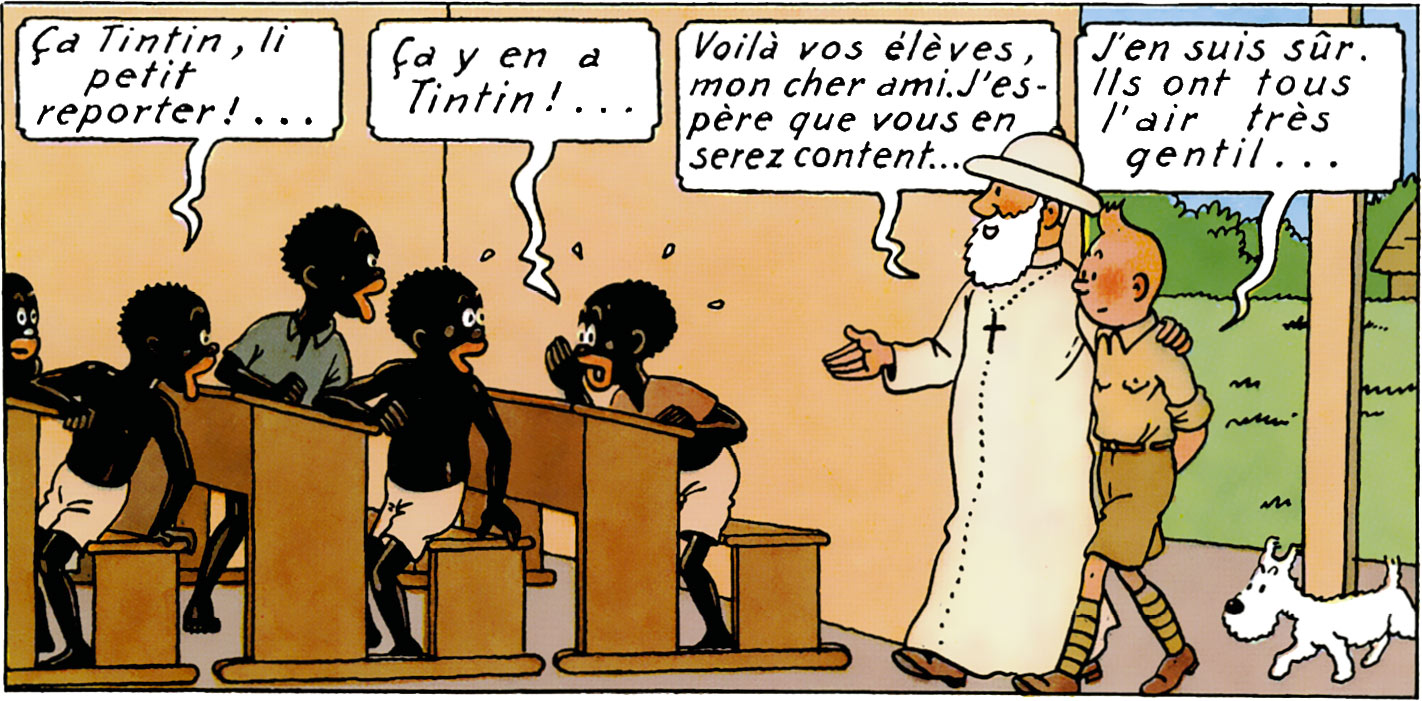
\includegraphics[width=\textwidth]{SeminaireMission/images/TintinCongo.jpg}

\paragraph{Un vocabulaire de conquête} "Position déjà acquise",.. le champ lexical est assez guerrier. 
Aujourd'hui, on n'emploie plus ces termes.



%--------------------------------------
\section{Rerum Ecclesiae}


\subsection{Présentation et biographie de l’auteur, Pie IX (1857-1939)}	

Pie XI, né Ambrogio Damiano Achille Ratti en Italie, est le Pape de l’entre-deux guerres (1922 à 1939). Si l’on jette un regard global sur son pontificat, très riche, c’est le Pape qui fait la transition entre chrétienté et monde moderne sécularisé. C’est certainement ce qui explique quelques paradoxes dans ses positions : 
\begin{itemize}
    \item  viscéralement anti communiste (il évoque dès sa 1ère encyclique, la lutte des classes comme « l’ulcère mortel des nations ») et il publie en mars 1937 \textit{Divini Redemtoris} qui condamne le communisme et le bolchevisme  ;  il sortira néanmoins une encyclique sociale\textit{ Quadragesimo anno} (QA) qui est la suite de \textit{Rerum novarum}, 40 ans après, dans laquelle il affirme le principe de subsidiarité. Dans ces 2 encycliques il confirme l’importance de mettre en place un syndicalisme chrétien et par ailleurs, il encourage la naissance de l’Action Catholique, notamment la JOC.                 \item La fête du Christ Roi, pour rappeler que le Règne de Dieu n'est pas à chercher dans un parti politique chrétien.
    
  \item  Dans 4 textes qui eurent un grand retentissement, il condamne le nationalisme exacerbé (Encyclique Ubi Arcano en 1922), l’action française (Allocution consistoriale en déc 1926), le fascisme (Encyclique Non abbiamo bisogno en 1931) et le nazisme (Encyclique \textit{Mit brenender sorge} mars 1937), et il sort ostensiblement de Rome quand Hitler vient dans la capitale italienne ; MAIS il s’entend néanmoins avec Mussolini avec qui il met fin à la querelle de Rome en signant en 1925 les accords du Latran. 
  \item  Sa vision de la religion est dit « intégraliste » c’est-à-dire que 
  
  \begin{quote}
      « son catholicisme intégral se conçoit comme une contre-culture alternative tant au libéralisme qu’au socialisme apportant ses propres réponses aux besoins de la société contemporaine, sans transiger avec la doctrine et les « erreurs [du] temps », autrement dit avec le modernisme. »
  \end{quote} Il freine par ailleurs des 4 fers l’ouverture de l’Eglise vers l’œcuménisme en ayant une vision unioniste, MAIS il prêche une égalité parfaite entre toutes les races, il évoque « l’universelle famille humaine » des peuples, qui « sont liés entre eux par des rapports de fraternité » (Ubi Arcano en 1922) et qui ont droit au respect, à la vie, à la prospérité, à la justice, et à la paix. Et devant le risque que représente la traque nazie des juifs, il n’hésite pas, selon la formule qui fera florès à se qualifier de « sémite ». 

  
\end{itemize}

Difficile donc de classer ce Pape, d’autant qu’au bout du compte, il restera surtout comme « le pape des missions » , comme nous allons le voir à présent.


\paragraph{Actions sur les missions}
\begin{itemize}
    \item Centralisation de l'oeuvre de mission de Pauline Jaricot à Rome (financement). Il cherchera à formaliser la machine financière.
    \item ordination des évèques chinois
    et japonais
    \item Ste Thérèse de l'Enfant Jésus, patronne des missions.
\end{itemize}



\subsection{Bibliographie consultée pour l’exposé}
 	

1.	Pie XI, Encyclique Rerum Ecclesiae sur les missions catholiques, 28 février 1926
2.	Benoit XV, Lettre apostolique Maximum illud, 1919
3.	BOUCHER André (Mgr)/ Institut Pie XI, L’action missionnaire, Paris, Librairie Bloud \& Gay, 1931, 226p
4.	PRUDHOMME Claude, « Chapitre 23 - La France et les missions catholiques, XVIIIe-XXe siècles » (p 375 à 390) in Alain Tallon \& Catherine Vincent (Sous dir), Histoire du christianisme en France, Collection U, Armand Colin, 2014, 448p 
5.	BRIA (Ion), Philippe CHANSON, Jacques GADILLE \& Marc SPINDLER, Dictionnaire œcuménique de missiologie – cent mots pour la mission ; Articles « 11 Clergé indigène (p50 à53) » par Paule Brasseur« 12 Colonisation (p53 à 56)» par J.Françis Zorn \& « « 69 Papauté et missions (p252 à 255) » par Claude Prudhomme, Paris CERF/Genève Labor et Fides/Yaoundé CLE, 2001, 394p
6.	DELACROIX (ss dir Mgr), Histoire universelle des Missions catholiques- T3 Les missions contemporaines (1800-1957) ; Chap 5 « l’avènement des jeunes églises Benoit XV, Pie XI et Pie XII » (p126 à 165), Paris, Librairie Grund, 1957, 447p
7.	COSTANTINI Cardinal, Réforme des Missions au XXème siècle, Paris, Casterman, 1960, 282p
8.	DESOUCHE Marie-Thérèse, « Pie XI, le Christ Roi et les totalitarismes » Dans Nouvelle revue théologique (Tome 130), 2008/4 , p 741 à 759
9.	ESSERTEL Yannick, Evangélisation et cultures – Essai d’histoire et d’anthropologie d’une pédagogie missionnaire du 1er au XXème siècle, CERF Patrimoines, 554p, 2021, Cote 297 411
10.	OOMS Toon, « Une ère nouvelle pour les missions - Le plaidoyer de Jean Bruls (1911-1982) pour un nouveau modèle missionnaire », dans Nouvelle revue théologique 2022/3 Tome 144, pages 452 à 470
11.	HILDESHEIMER Françoise, Une brève histoire de l'Église - Le cas français IVe-XXIe siècles ; chap9 « Modernistarum callidissimum artificium »,  Coll. Champs Histoire, Flammarion, 2019, 477p
12.	Ouvrage collectif, Théo – Nouvelle encyclopédie catholique, Droguet-Ardant/Fayard, 1989, 1236p
13.	Site du Vatican, notamment consultation des biographies des papes Benoit XV, Pie XI, Pie XII
14.	WIKIPEDIA, articles « Missions catholiques aux XIXe et XXe siècles » ; « Benoit XV » ; « Pie XI » ; « Pie XII » ; « encyclique Rerum Ecclesiae » « Lettre apostolique Maximum illud »


\subsection{Nature du texte et contexte historique et textuel}
 

L’Encyclique Rerum Ecclesiae est la 8ème encyclique de Pie XI, Pape particulièrement prolixe en encycliques  . C’est, nous l’avons dit, le « Pape des missions ». Il intervient dans une période particulièrement intense :  le personnel missionnaire passe de 1903 à 1925 de 15000 à 30000. Tout est doublé : les missions, les baptisés. Le Pape se sent donc appelé à organiser ces missions. Particulièrement actif dans les 8 premières années de son pontificat, il adopte une attitude presque militaire en centralisant dès la 1ère année de son pontificat, à Rome, en 1922, l'Œuvre de la Propagation de la Foi (créée par Pauline Jaricot à Lyon). En 1923, c’est la constitution des premières églises indigènes aux Indes et l’année d’après, le concile plénier de Shanghaï. Et en décembre 1924, il organise l’exposition missionnaire du Vatican temporaire (jusqu’au 10 janvier 1926) qui deviendra ensuite permanente, comme il le dit explicitement dans l’encyclique (création en novembre 1926 d’un musée ethnologique des missions au palais du Latran). Puis sort le 28 février 1926 l’encyclique Rerum Ecclesiae. Soucieux de l'ouverture du clergé aux indigènes, il sacre en 1926 les six premiers évêques chinois et l’année suivante le 1er Evêque japonais. Et fin 1927 il institue Ste Thérèse de Lisieux comme patronne des missions. Enfin en 1929, il réorganise et coordonne l’action de ses 3 grands instruments de la Mission, conformément à ce qu’il annonce dans l’encyclique Rerum Ecclesiae : les grandes œuvres pontificales de la propagation de la Foi (qui subvient aux besoins généraux de la Mission) ,  la Sainte Enfance (qui s’occupe des enfants des pays de mission) et St Pierre-apôtre (qui met en place et prend en charge les séminaires et la formation des prêtres indigènes). 

\subsection{L’encyclique}
\paragraph{L’objet et l’effet recherché}

C’est dans le contexte décrit précédemment que s’inscrit l’encyclique Rerum Ecclesiae. Elle porte le sous-titre suivant : « sur le développement à donner aux missions ». Elle s’adresse donc en premier chef aux responsables de Mission et de façon générale à tous les missionnaires. Mais cela va au-delà car Pie XI souhaite mobiliser tous les catholiques.
Il s’agit essentiellement premièrement de « booster » les missions en impliquant tout le peuple catholique ; il s’agit, deuxièmement, de réfléchir à la mise en place d’une part et à la formation, d’autre part, d’un clergé indigène à vaste échelle.


On ressent une certaine urgence dans cette encyclique : Pie XI se vit clairement comme un pape dont « le but [est] de répandre la lumière de l’Evangile et les bienfaits de la culture et de la civilisation chrétiennes aux peuples qui "étaient assis dans les ténèbres et dans l’ombre de la mort" », pour reprendre le tout début de son encyclique (§1).  


L’enjeu majeur, pour l’Eglise, en effet, c’est à la fois de développer, mais aussi de pérenniser ces avancées missionnaires sur des terres nouvellement christianisées. 
Le contexte missionnaire est le suivant : implicitement, en Afrique, en Asie,  les religions sont clairement en concurrence les unes les autres et il est clair que Pie XI ne souhaite se faire doubler ni par l’islam, ni par les protestants. L’heure n’est ni à l’œcuménisme (en tous cas, avec son approche unioniste, le Pape est très réticent vis-à-vis des prises d’initiatives qui se font jour) ni au dialogue interreligieux. Mais explicitement, c’est contre le paganisme qu’il se bat : il déplore le fait que les païens soient quasi 1 milliard (§4)

\paragraph{L’argumentation }
 

Souvent, l’Eglise est assimilée au colonisateur. Il y a donc un grand risque que celle-ci soit considérée comme une occupation étrangère par des missionnaires occidentaux. D’où l’urgence ressentie par le Pape de développer et former un clergé insulaire. Pie XI, pour le dire, reprend l’image de la vigne : « Pourquoi le clergé indigène serait-il empêché de cultiver son champ ? ». 

De plus, il se joue aussi un enjeu qui a à voir avec une certaine vision humaniste. De même que Lavigerie a été à la pointe du combat contre l’Esclavage, il est nécessaire de se battre aussi pour parvenir à une totale égalité entre le clergé européen et le clergé insulaire. C’est ce qu’évoque le Pape en parlant de stricte égalité dans la « dignité sacerdotale ».  Mais est-ce vraiment l’argument humaniste qui l'emporte ? N'est-ce pas plutôt une forme de réalisme au nom de l’efficacité missionnaire ? 
Car Pie XI reprend dans son encyclique un argument de Benoit XV figurant dans Maximum Eliud : 

\begin{quote}
    « le prêtre, par sa naissance, son tempérament, ses sentiments et ses intérêts est en contact étroit avec son propre peuple, il est au-delà de toute controverse à quel point il peut être précieux pour inculquer la Foi dans l’esprit de son peuple. Le prêtre autochtone comprend mieux que n’importe quel étranger comment procéder avec son propre peuple. » (§21). 
\end{quote}
Il rajoute un argument supplémentaire qui va dans le même sens : la connaissance imparfaite de la langue.

Par ailleurs, est pointé aussi le fait que l’Europe a elle aussi besoin de ses prêtres (23§). Il est d’ailleurs intéressant de noter cet argument à la lumière du 3ème texte étudié aujourd’hui de Pie XII : \textit{Fidei Donum} qui donnera à l’inverse la possibilité aux prêtres diocésains à répondre aux appels des missions d'outremer, notamment en Afrique et Amérique latine, tout en restant attachés à leur diocèse d'origine.

Le gros du développement du texte (à partir du §19), et le plus important, est consacré à la formation et au statut de ce clergé indigène. Il est affirmé -ce qui ne va pas de soi au moment où sort l’encyclique-  l’égalité dans la formation initiale, l’égalité dans les responsabilités, dans les missions données aux uns et aux autres. Et surtout, il est clairement préconisé l’ouverture de séminaires sur place. Il faut instruire les séminaristes indigènes de toutes les sciences modernes (sciences sacrées et profanes » est-il précisé §21). 

Pie XI évoque aussi l’opportunité de la création « de congrégations entièrement nouvelles, qui correspondraient mieux au génie et au caractère des indigènes et qui seraient plus en accord avec les besoins et l’esprit des différents pays. » Cela ne l’empêche pas de donner la Possibilité pour les indigènes de rallier des congrégations anciennes y compris des contemplatifs. 

Enfin il souhaite optimiser l’organisation de la mission, et implanter le christianisme en créant sur place des écoles, des hôpitaux, etc… 

 \paragraph{La valeur théologique du texte : une christologie de conquête et une ecclésiologie missionnaire qui s’inscrit dans la durée}


Le vocabulaire est un vocabulaire de conquête, somme toute pas très loin de l’expansionnisme colonial. Il s’agit de « gagner au Christ tous ceux qui ne le connaissent pas ou sont encore sans troupeau. »  Dans cette vision, le Pape se considère comme le « vicaire du Christ » (cela a été dit par Pie XI dans des discours)
Notons au passage au §5 un passage qui éclaire la vision intégraliste du Pape et qui témoigne d’une christologie très particulière : il importe pour lui en effet : « que nous essayions de mettre sous la domination du doux Christ autant d’autres hommes que possible ». Le Pape et partant l’Eglise en mission, s’apparentent à une armée. La christologie de Pie XI est fondée sur une vision hiérarchique au sommet de laquelle il y a le Christ. Et juste en dessous le Pape.  On rappelle que c’est Pie XI qui a instauré en 1925 la célébration du Christ-Roi qui met en avant la puissance du Jésus-homme …Toutefois il ne s’agit pas de prendre les armes mais de convertir. Et pour cela est mise en avant « l’autorité particulière du Pape sur les missions. » . Pie XI se situe clairement toujours dans une logique de chrétienté, mais ce sont bien les derniers soubresauts qui tomberont après la 2 GM.


Par ailleurs, concernant l’Eglise, ce qui est fondamentalement en jeu, c’est un changement de paradigme ecclésiologique et missionnaire : il s’agit d’avoir une vision de la Mission qui soit une approche temporaire, un état transitoire et passager. Il n’est plus question que s’implantent durant des siècles, comme cela avait pu se passer auparavant, des missionnaires étrangers qui s’inculturent. On n’en est plus là. Les missionnaires ont vocation à tout mettre en œuvre pour que se développe et se mette en place un clergé indigène, autochtone qui pourra, si on peut dire, passer la 2ème couche de l’évangélisation.
\paragraph{"Apporter la civilisation Chrétienne"} Vocabulaire qu'on n'utiliserait pas aujourd'hui mais qui inclut aussi les oeuvres - éducation, medecine .   

\begin{quote}
   
 p. 2 : idée de culture chrétienne.

« la dette de charité qui nous lie à Dieu exige non seulement que nous nous efforcions d'augmenter le nombre de ceux qui le connaissent et l'adorent " en esprit et en vérité " [3], mais encore que nous soumettions le plus grand nombre d'entre nous au règne du très aimable Rédempteur, afin que " l'utilité de son sang " [4] soit chaque jour plus féconde, et que nous lui soyons de plus en plus agréables, tandis qu'il lui plaît par-dessus tout que les hommes soient sauvés et parviennent à la reconnaissance de la vérité [5]. »

\end{quote}
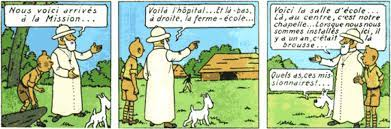
\includegraphics[width=\textwidth]{SeminaireMission/images/TintinCongo2.jpg}

\paragraph{Changement de vision sur la culture} Musée missionnaire avec les arts locaux
\paragraph{Continuité d'un certain vocabulaire de Maximum Illud}
\begin{quote}
    p. 10 
« « Il est bien vrai que la parole de Dieu et ses prédicateurs sont plus facilement reçus par les plus humbles roturiers ; il est vrai aussi que Jésus a dit de lui-même : " L'Esprit du Seigneur... m'a envoyé évangéliser les pauvres "[19] ; mais outre le fait qu'il faut se rappeler la parole de saint Paul : " Je suis redevable aux sages et aux insensés "[20], la pratique et l'expérience nous enseignent qu'une fois que les chefs du peuple ont été conduits à la religion du Christ, les classes les plus humbles suivent facilement. »
\end{quote}


Faut-il l’option préférentiel pour les pauvres ou alors toucher l’ élite ?
\begin{quote}
    
\end{quote}
« Les territoires confiés par le Saint-Siège à vos soins assidus, afin que vous les placiez sous la loi du Christ, sont pour la plupart d'une grande étendue. »

Logique territorial , RdD : sous la Loi du Christ.


\subsection{ Appréciation et discussion critique}
 

Il s’agit d’une encyclique qui amplifie, précise et applique la lettre apostolique du prédécesseur de Pie XI, Benoît XV Maximum Illud (du 30 novembre 1919 ) considérée comme « la grande charte des missions modernes ». Il y a donc beaucoup d’idées qui se trouvaient déjà en germe dans ce premier document comme la formation d’un clergé insulaire. Mais qui sont précisées. 


\paragraph{En chiffre}
Si l’on fait un bilan de la situation dans les années 30, soit 5 ans après cette encyclique, selon le livre L’action missionnaire, on parvient aux chiffres suivants : 3734 prêtres indigènes et 8279 prêtres étrangers soit 31\% d’autochtones. On voit donc que la politique que veut faire triompher Pie XI ne se concrétise pas massivement dans les faits. Elle sera stoppée par l’ouragan de la seconde guerre mondiale puis de la décolonisation.

Et si l’on prend, pour finir, un regard contemporain, force est de constater que dans tous les pays du monde à présent, se sont mis en place des clergés et des séminaires autochtones. On peut donc dire que de ce point de vue la vision de Pie XI a, de ce point de vue, triomphé.  Un triomphe tel que, par une totale ironie de l’histoire, c’est à présent ce "clergé indigène" -pour conserver un titre qui a extrêmement mal vieilli- qui vient aujourd’hui au secours des paroisses françaises ; et qui, sans lui, faute de vocation sacerdotale dans notre pays, ne seraient plus en mesure de fonctionner…               
 

\paragraph{Question sur la motivation du clergé autochtone} Est ce pour l'efficacité de la mission ou par vision égalitariste ?


\section{Fidei Donum}
Ce sont les deux mots latins en tête de l'encyclique du Pape Pie XII du 21 avril 1957. Fidei Donum. don de la foi. Ce sont les deux mots latins en tête de l’encyclique du Pape Pie XII du 21 avril 1957 intitulée « Fidei Donum » invitant les évêques à porter avec lui « le souci de la mission universelle de l’Eglise », non seulement par la prière et l’entraide, mais aussi en mettant certains de leurs prêtres et fidèles à la disposition de diocèses d’autres continents. Les prêtres envoyés, restent attachés à leur diocèse d’origine et y reviennent après plusieurs années passées en mission. On les appelle souvent « Prêtres Fidei donum.»

\paragraph{Un vocabulaire daté}
\begin{quote}
    Any delay or hesitation is full of danger. For the people of Africa have made as much progress toward civilization during the past few decades as required many centuries among the nations of Western Europe. Thus they are more easily unsettled and confused by the introduction of theoretical and applied scientific methods, \textbf{with the result that they tend to be unduly inclined to a materialistic outlook on life}. Hence a condition of affairs is sometimes brought about that is difficult to correct and in the course of time may prove to be a great obstacle to the growth of faith, whether in individuals or in society at large. For this reason it is imperative that help should be given now to the shepherds of the Lord's flock in order that their apostolic labors may correspond to the ever-growing needs of the times.
\end{quote}


 \begin{quote}
     57. Nous pourrions nous demander, en outre, si nos prières viennent d'un cœur sincère si nous prions pour le succès des missions sans accompagner nos prières d'offrandes charitables selon nos moyens. Nous connaissons bien - en fait, mieux que quiconque - la libéralité abondante de Nos fils, comme en témoignent constamment de nombreux exemples merveilleux. A ces âmes généreuses est due, sans aucun doute, le merveilleux essor de nos missions depuis le début de ce siècle. En conséquence, nous désirons exprimer notre profonde gratitude à nos fils et filles bien-aimés qui contribuent par leurs efforts zélés et leur soutien caritatif à de nombreuses entreprises missionnaires.
 \end{quote}

 \begin{quote}
63. L'Église en Afrique, ainsi que dans d'autres parties du champ missionnaire, a besoin de missionnaires. C'est pourquoi Nous vous appelons une fois de plus, Vénérables Frères, en vous priant de faire preuve de zèle avec toutes les ressources dont vous disposez pour soutenir tous ceux qui ont été divinement appelés à assumer les charges de l'apostolat missionnaire, qu'ils soient prêtres ou religieux et femmes.
     
 \end{quote}

 \paragraph{Etudiants africains}
 \begin{quote}
     71. Avec le même intérêt affectueux qui joint ses efforts à ceux des autres dans une harmonie fraternelle et exclut toute considération égoïste, veillez particulièrement à accorder un soin spirituel aux jeunes d'Afrique et d'Asie, qui résident peut-être dans vos diocèses en vue de leur poursuivre leurs études.

72. Ces jeunes hommes, déracinés par les bouleversements sociaux dans leur propre pays, n'ont souvent pas, pour de nombreuses raisons, suffisamment de contacts sociaux catholiques parmi les personnes qui les accueillent. De ce fait, leur vie chrétienne peut être mise en danger, car les vraies valeurs et excellences de la nouvelle culture qu'ils recherchent peuvent leur échapper et ils peuvent, en conséquence, être séduits par les doctrines du matérialisme et succomber aux flatteries des coteries athées. Vous ne pouvez pas ignorer l'impact de cela sur leur carrière actuelle et future. Ce serait une bonne idée de nommer des membres du clergé dévots et bien équipés pour prendre en charge cet apostolat, soulageant ainsi les inquiétudes de leurs propres évêques dans les champs de mission.
 \end{quote}

 \paragraph{Regard égalitariste entre les jeunes églises} 

 \paragraph{Solidarité entre Eglises} Don à court terme d'un prêtre et non jusqu'à la mort. Temps limité du prêtre au service de l'Eglise. 

\paragraph{Civilisation chrétienne}


un contexte marxiste anti-religieux.


  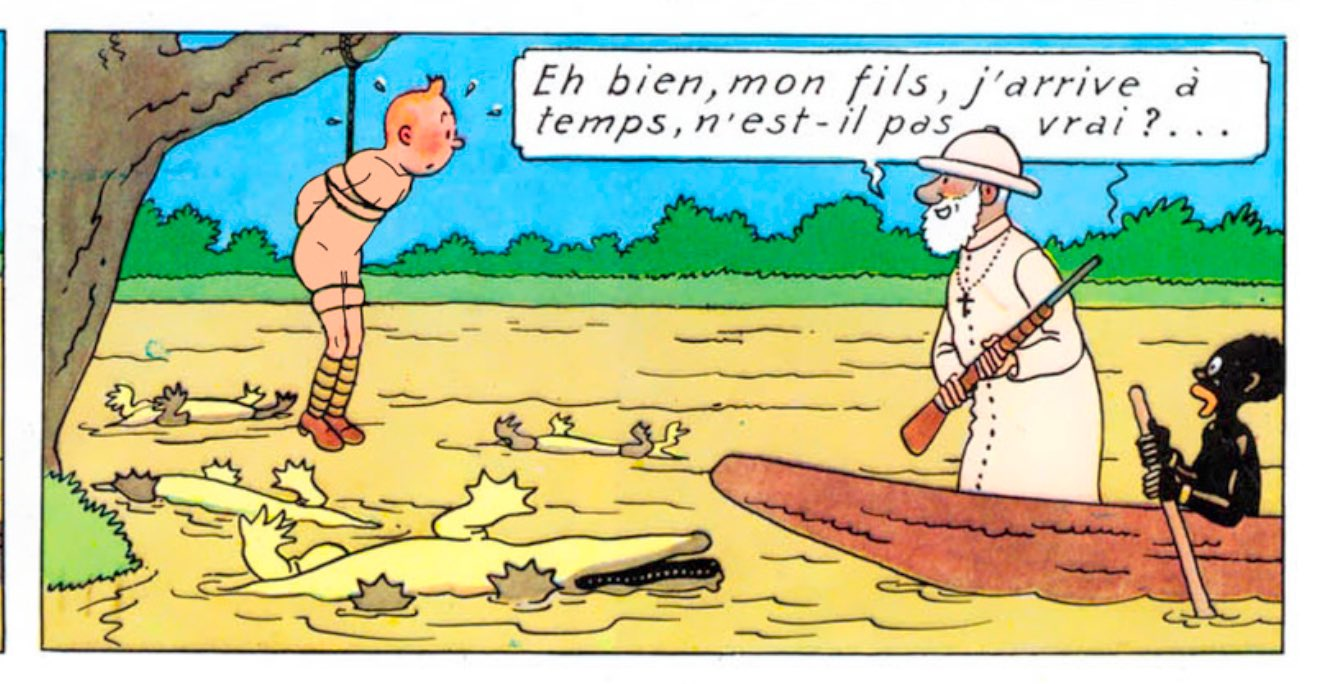
\includegraphics[width=\textwidth]{SeminaireMission/images/TintinCongo3.jpg}  


 
\section{Bilan}

\paragraph{sur la forme} du séminaire
Démarche chronologique pertinente. Continuité et modification.
distance avec ces textes, y compris de Vatican II.

\paragraph{sur le fond} prendre deux ou trois points que nous retenons de ce séminaire.

Mission : dialogue, nous force à creuser notre foi.

Occasions manquées, en particulier avec FX et Matteo Ricci.

Marie de l'Incarnation, bonne surprise et le plan pour le Quebec.

Question ouverte : sur la figure du prophète, qui détruit les idoles, et la figure sapientielle de l'ouverture aux autres. FX : actualité, dans Laudato Si.  





\chapter{Ad Gentes - Concile Vatican II}


\section{Préparation}
\paragraph{Plan}
Préambule (1)

Principes doctrinaux (2-9)

L’œuvre missionnaire elle-même (10-18)
\begin{itemize}
    \item Introduction (10)
  \item Le témoignage chrétien (11-12)
  \item La prédication de l’Évangile et le rassemblement du Peuple de Dieu (13-14)
  \item La formation de la communauté chrétienne (15-18)
\end{itemize}
 
Les Églises particulières (19-22)

Les missionnaires (23-27)

L’organisation de l’activité missionnaire (28-34)

La coopération (35-41)

Conclusion (42)

\subsection{Lecture attentive}
\begin{itemize}
    \item \paragraph{Principe doctrinaux} : 
    \begin{itemize}
        \item  Dieu veut nous rassembler en un peuple\mn{Jn 11, 52 Et ce n'était pas pour la nation seulement; c'était aussi afin de réunir en un seul corps les enfants de Dieu dispersés.}
        \item la mission du fils : Dieu s'engage dans l'histoire humaine.
        \item Mission du saint esprit : \textit{pousse l'Eglise à s'étendre. }
        \item l'Eglise envoyée par le Christ.  \textit{C'est de là (Allez baptiser...) que découle pour l'Eglise le devoir de propager la foi et le salut apportés par le Christ. } 
        \item l'activié missionnaire : Évêques.  \textit{la mission est unique et la même partout, en toute situation, bien qu'elle ne soit pas menée de la même manière du fait des circonstances}
    \end{itemize}
   \item les Eglises particulières
    
\end{itemize}

\paragraph{Rôle des évêques} Après des textes sur l'activité missionnaire centralisée, rôle des évêques. Car la mission ne se pense plus comme les \textit{missions} (quand il n'y a pas d'Eglise en un lieu)

\paragraph{Insistance à l'universalité} \textit{la mission est unique et la même partout, en toute situation, bien qu'elle ne soit pas menée de la même manière du fait des circonstances} -6)

\begin{quote} AG 16
    Ces exigences communes de la formation sacerdotale, même pastorale et pratique, selon les dispositions du Concile [47], doivent se combiner avec le zèle à prendre en considération le mode particulier de penser et d’agir de son propre peuple. Les esprits des élèves doivent donc être ouverts et rendus pénétrants pour bien connaître et pouvoir juger la culture de leur pays ; dans les disciplines philosophiques et théologiques, ils doivent saisir les raisons qui créent un désaccord entre les traditions et la religion nationales, et la religion chrétienne [48]. De même, la formation sacerdotale doit tenir compte des nécessités pastorales de la région ; les élèves doivent apprendre l’histoire, le but et la méthode de l’action missionnaire de l’Église, et les conditions particulières d’ordre social, économique, culturel de leur propre peuple. Ils doivent être éduqués dans un esprit d’œcuménisme et préparés comme il convient au dialogue fraternel avec les non-chrétiens [49]. 
\end{quote}


\paragraph{Transformation} Il n'est pas rare que les groupes humains au sein desquels l'Eglise existe, ne soient complètement transformées pour des raisons diverses. des situations nouvelles peuvent en résultaer (6)

\paragraph{Divisions des chrétiens} 6

\begin{Synthesis}
    L’activité missionnaire n’est rien d’autre et rien de moins que la manifestation du dessein de Dieu, son épiphanie et sa réalisation dans le monde et son histoire, dans laquelle Dieu conduit clairement à son terme, par la mission, l’histoire du salut. 9
\end{Synthesis}

% \chapter{Lire les classiques Chinois}

 

\textbf{Comment lire les classiques chinois ? (French Edition)}

\textbf{Vermander, Benoît}

\section{Prologue}


\subsection{Période axiale}
  \mn{ p. 5 · E. 59  } \begin{quote}
Lorsque la notion même de « période axiale » est acceptée au moins comme
hypothèse de travail ( elle est parfois rejetée dès l'abord ) , les
percées qu'on lui associe sont généralement les suivantes : ( a ) les
penseurs de la période auraient contribué à « problématiser le monde »
plutôt qu'à le recevoir tel quel , ce par le fait d'articuler la réalité
sociale autant que naturelle autour de questions portant sur son «
pourquoi » et son « comment » ; ( b ) c'est ainsi qu'aurait émergé la «
conscience critique » , l'examen des opinions reçues , la remise en
cause d'au moins certaines des structures sociales ; ( c ) ce
questionnement
aurait nourri un souci éthique ( à moins que ce dernier ait contribué à
l'émergence de la conscience critique ) , souci qui fut accompagné
souvent de la formation d'une vision utopique -- la cité idéale de
Platon , la pleine libération des individus dans le bouddhisme , le rêve
d'un ordre social gouverné par les rites , l'éducation morale , chez
Confucius , l'annonce de la venue du Royaume de Dieu chez les prophètes
d'Israël ; ( d ) le surgissement critico - éthique aurait été porté par
des personnalités incarnant les « sauts » entrepris , personnalités dont
le nom est transmis aux générations qui leur succèdent ; ( e ) ces
personnalités sont souvent représentées ( et semblent s'être considérées
elles - mêmes ) comme des « Renonçants » , des individus dont les choix
de vie mettent en question l'ordre dominant : dans la République , le
philosophe de la cité idéale de Platon renonce aux possessions privées
et à la vie de famille pour gouverner la Cité avec justice

\end{quote}  

\subsection{Divination, mathématique et concepts}
\mn{- p. 17 · E. 258  } \begin{quote}  

Élaborer des ramifications entre les principaux viscères du corps humain
et les états climatiques ( le chaud , le froid , le sec , l'humide ) ,
les émotions , les notes de musique , les couleurs , tout cela transcrit
dans une arithmétique de
base cinq » , n'est pas simple opération de l'esprit mais permet bien
d'observer pragmatiquement un ensemble de correspondances . En même temps, ces analogies deviennent moralement signifiantes. C’est ainsi que s’opère une évolution du divinatoire au combinatoire et à l’éthico-politique.   
A la fois matrice de ce processus et l'accompagnant tout au long de sa
formation textuelle , le \textit{Classique des mutations ( Yijing )} construit un
métalangage de l'univers à partir d'une réflexion mathématisée sur les
processus de divination.
il s'essaie à décrire la façon dont les phénomènes se suivent et
s'agencent de façon nécessaire . C'est , à l'extrême , une mathématique
de tous les phénomènes possibles , fondée sur l'idée que tout n'existe
que dans l'échange , le passage , la fluidité : la gradation est un
autre nom du contraste , et la logique des transformations ( des
changements par quoi une forme entre en contraste avec celles qui la
précèdent et la suivent ) , non pas celle des oppositions , régit
l'univers et la pensée .

\end{quote} \mn{ p. 18 · E. 268 } \begin{quote}

Au ciel se composent les images {[} xiang {象} {]} , sur la terre se
composent les formes {[} xing 形 {]} , et les transformations se font
visibles {[} Yijing , Xici 繫辭 I . 1 {]} 28 .

\end{quote} 

\paragraph{le rite comme éducation} chez Confucius
\mn{p. 20 · E. 304  } \begin{quote}

Le vecteur de l'éducation ainsi dispensée , ce sera le rite
: l'éducation de l'intérieur par l'extérieur . À noter pourtant que « le
rite » ( chinois ) et « la loi » ( en contexte grec ou hébreu ) ne se
trouvent pas dans un strict régime d'opposition : ils régulent tous deux
les conduites extérieures jusqu'au moment où les prescriptions se
retrouvent être inscrites « au fond des cœurs » .

\end{quote} \mn{ p. 24 · E. 367 } \begin{quote}

La détermination d'un corpus de classiques fonde une culture dans sa
spécificité tout en lui donnant d'affirmer son l'universalité latente .
Hans - Georg Gadamer fait de l'extensibilité ,  en principe illimitée, de la durée pendant laquelle une œuvre communique son sens le trait qui désigne un « classique »
\end{quote} 
 
\section{Chapitre I : Qu'est-ce qu'un classique chinois ?}

\mn{ p. 37 · E. 786 } \begin{quote}

Du reste , dès les premiers rencontres entre lettrés chinois et
missionnaires occidentaux , les uns et les autres comprennent que le
continent qui leur fait face est fondé sur une armature de classiques
dont la maîtrise est essentielle pour la réussite culturelle ,
religieuse et sociale , et ils feront de la connaissance réciproque de
ces textes la clé d'une rencontre possible , d'une entrée dans la pensée
de l'Autre , que ce soit pour l'apprécier ou l'utiliser , pour
convaincre ou dominer l'interlocuteur .

\end{quote} \mn{p. 38 · E. 805  } \begin{quote}
On trouve cette acception chez Yang Xiong 揚雄 (53 AEC-18) :

 
 \begin{quote}
     : « Un texte qui ne se mesure pas aux Classiques n’est pas un texte. Une parole qui ne se mesure pas aux Classiques n’est pas une parole. Ce sont des excroissances qui prolifèrent  
 \end{quote}
La formule, très concise, pourrait aussi être comprise comme signifiant : « Un texte qui n’est pas (qui ne tend pas au) Classique n’est pas un texte. » Ou même plutôt : \textit{« Un texte non référé à une norme n’en est pas un. »} Le registre sémantique du passage 11 rappelle celui qui entoure le terme déjà évoqué κανών : l’instrument qui norme (la règle du charpentier en grec) donne naissance à un ensemble textuel établi par rapport à lui – ensemble qui, de normé, devient alors normatif.
 
\end{quote} \mn{p. 44 · E. 926  } \begin{quote}

Pouvoir {[} di {]} d'en haut {[} shang {]} » surplombe le monde
surnaturel ( ne parlons pas d'un « panthéon » ,car on n’y trouve pas l’individuation des divinités qu’on attache d’ordinaire à ce terme).

 

\end{quote} \mn{ p. 45 · E. 951 } \begin{quote}

L'autre chapitre des Documents sur lequel nous nous arrêterons
brièvement est celui du Hongfan 洪 範 , expression que l'on peut
traduire par « Grand plan » ou , sans doute plus justement , par «
Modèle universel » . Il présente l'ensemble des phénomènes ( éléments ,
conduites , matières politiques , calendrier , sources de bonheur et
malheur ) sur des combinaisons fondées sur les chiffres Cinq et Neuf .
Sa composition apparaît si rigoureuse que certains formalistes russes
ont spéculé sur son nombre de caractères et leur inscription à
l'intérieur d'un carré magique 30

\end{quote} 

\paragraph{les annales historiques} attribuées à Confucius : essayer de dicerner les signes des temps. 
\mn{ p. 56 · E. 1164 } \begin{quote}
les lecteurs de ces Annales vont s’employer à faire émerger des sens, à trouver l’expression du mandat du Ciel dans cette succession d’événements qu’ils vont lire comme une sorte de rébus. C’est dire que ce sont les commentaires suscités par l’œuvre qui en font tout l’intérêt.
[..]
Au travers de la sèche prose des Printemps et
  Automnes , le Gongyang s'emploie à trouver « le sens profond de paroles
subtiles"
\end{quote}


Importance du processus de mémoire.

 \mn{p. 59 · E. 1228  } \begin{quote}

Au travers de cet hommage rendu par les historiographes du Zuozhuan à
leurs prédécesseurs se donne à lire leur conviction : l'enregistrement
et la qualification fidèles des événements sont questions de vie ou de
mort . Cela parce que l'enchaînement des actions , des prédictions que
l'on en tire , de la vérification ou non de ces prédictions constitue la
trame de l'ordre du monde , et qu'en altérer le récit , c'est forcément
en distordre la marche .

\end{quote}

\paragraph{Anectdote : matériau de la connaissance historique} car elle offre un aperçu soudain sur une réalité plus profonde et étendue, comme la citation. \mn{ p. 59 · E. 1233 } \begin{quote}
Du fait de la nature même de ces deux extraits, on aura noté la place que joue, dans le Zuochuan, le genre littéraire très particulier de l’anecdote.
 
Elle est révélatrice d'une tendance plus générale : l'anecdote , dans
l'historiographie chinoise , deviendra le matériau même de la connaissance historique.
 

\end{quote} 
\subsection{le sacrifice comme lieu de l'unité}
Une partie des textes classiques visent à expliquer la tenue en cas de non respect du sacrifice. Cette importance peut étonner.
\mn{p. 65 · E. 1345  } \begin{quote}

C'est en distinguant qu'on peut droitement unir .
Le

mode de découpe de l'animal sacrifié puis la façon dont on répartit les
parties découpées constituent des opérations destinées à symboliser et
réaliser la cohésion du groupe , dans un modèle qui associe exigence
d'unanimité et affirmation de principes hiérarchiques stricts . 

\end{quote} \mn{ p. 66 · E. 1353 } \begin{quote}
Le sacrifice
était donc image inversée de l'ordre social effectif . La supériorité
sociale était étroitement associée à la capacité de donner .

\end{quote} \mn{  p. 66 · E. 1356 } \begin{quote}

Les anomalies rituelles relevées par les textes fonctionnent alors comme
informations historiques d'importance particulière . La crise rituelle
est toujours symptôme de crise politique .

\end{quote} \mn{ p. 66 · E. 1357 } \begin{quote}

le Liji traduit une anxiété face à tous les dysfonctionnements possibles
de l'activité rituelle , et , de ce fait , du travail social .

\end{quote} \mn{p. 67 · E. 1368  } \begin{quote}

Le rituel est donc affecté par une tension entre son but avoué -- édifier ,
maintenir un ordre -- et le fait qu'il soit par essence une entreprise
risquée , soumise à divers aléas .

\end{quote} 
\subsection{La grande Etude - Daxue}
\mn{p. 67 · E. 1384  } \begin{quote}

Tentons après tant d'autres une traduction de cette célébrissime entrée
en matière -- sachant qu'aucun lecteur ni commentateur n'arrive à faire
vraiment abstraction de la lecture qu'en ont effectué Zhu Xi et ses
continuateurs . 
\begin{quote}
    La voie de la Grande Étude 96 , c'est d'éclairer {[} le
principe de {]} vertu qui {[} lui - même {]} éclaire {[} toute chose {]}
, c'est d'aimer {[} ou bien de « renouveler » , selon les versions {]}
le peuple , et c'est de ne s'arrêter qu'une fois la plus haute
perfection atteinte . Sachant le terme , on prend sa détermination . Une
fois déterminé , on peut s'apaiser {[} jing 靜 97 {]} . Une fois apaisé
, on peut s'ancrer dans la paix . Quand on est ancré dans la paix , on
peut discerner . Ayant discerné , on peut atteindre le but . Les plantes
ont racine et branches , les affaires un commencement et une fin . Celui
qui sait la succession des affaires , il est tout proche de la voie .
大學之道,在明明德,在親[新]民,在止於至善。知止而后有定,定而后能靜,靜而后能安,安而后能慮,慮而后能得。物有本末,事有終始,知所先後,則近道矣。


\end{quote}


\end{quote} \mn{ p. 69 · E. 1411 } \begin{quote}

La partie gauche du caractère , sa clé sémantique , c'est le jade ( yu 玉 )
. Associée à l'autre partie du caractère , cette clé donne à l'ensemble
un tour plus abstrait : elle parle d'une structure sous - jacente aux
phénomènes qui prennent corps . Les Chinois ont trouvé dans les nervures
du jade la plus marquante des expressions des forces vitales qui , à
l'interne , structurent l'organisme.

\end{quote} 
\paragraph{L'invariable milieu, à l'autre extremité des quatre livres}
\mn{ p. 69 · E. 1420 } \begin{quote}
Comme pour la Grande Étude, voyons à traduire le premier paragraphe du texte :
\begin{quote}
La loi du Ciel 101, c’est ce qu’on appelle « la nature » 102. Se conformer à la nature, c’est ce qu’on appelle « la voie ».
\ldots

   Aussi , l'homme de bien se tient sur ses gardes même quand il ne
distingue rien {[} d'inquiétant {]} , il craint et tremble même quand
rien ne frappe son oreille . 
 
\ldots

Aussi , l'homme de bien reste sur ses gardes {[} même {]} dans la
solitude 104 . N'émettre {[} fa 發 {]} ni joie ni colère ni tristesse ni
allégresse , c'est ce qu'on peut appeler l'équilibre {[} le milieu {]} .

\end{quote} 
\end{quote}

Relecture

\paragraph{Xunzi : la discrimination fait l’homme
 }
\mn{ p. 72 · E. 1482 } \begin{quote}

On a argué , à mon sens fort justement , que le caractère fen 分 (
séparer , diviser ) constitue une clé -- sinon la notion clé -- du Xunzi
112 . Le fait que l'on compte 113 occurrences du caractère dans
l'ouvrage est un premier signe de son importance .

\end{quote} \mn{ p. 73 · E. 1493 } \begin{quote}

le principe de base sur lequel Xunzi fonde sa théorie politique est que
les désirs ( par essence subjectifs ) sont par nature illimités , tandis
que les biens sont objectivement limités ( yu duo er wu gua 欲 多 而 物
寡 113 ) . Savoir comment répartir et partager , c'est bien là l'essence
de l'art politique 114 . Xunzi pose ici l'accent sur la notion de gong
公 : gong ( habituellement traduit par « chose publique ») consiste à diviser quelque chose avec impartialité, sans afficher égoïsme ou partialité (si 私).
 

\end{quote} \mn{ p. 74 · E. 1510 } \begin{quote}
Le rituel, manifestation privilégiée des distinctions ainsi effectuées, devient alors le conduit par quoi ce qui était au départ
de l'ordre de la nature ( xing 性 ) se transforme en artifice ( wei 偽 )
, ce dernier terme revêtant un sens éminemment positif
 
\end{quote} 
Sens positif de l'artifice chez xunxi.
\begin{Def}[artifice]

\end{Def}
\mn{ p. 74 · E. 1522 } \begin{quote}

Xunzi trace une distinction entre les niveaux atteints respectivement
par le Lettré ( shi 士 ) , l'homme de bien ( junzi 君子 ) et le sage (
shengren 聖人 ) , ce dernier seul capable de fusionner en un tout la
perfection des dispositions à l'interne et celle atteinte par les
observances extérieures .



\end{quote}


Cf vie digne et vie parfaite

\mn{p. 75 · E. 1527  } \begin{quote}

Les châtiments contribuent à assurer l'équilibre entre hiérarchie et
impartialité .

\end{quote} \mn{ p. 76 · E. 1550 } \begin{quote}

Xunzi voyait bien la nature humaine ( xing 性 ) comme mauvaise ( e 惡 )
, il discernait dans l'artifice rituel couplé à la droite éducation la
route par laquelle s'ouvrait la possibilité de dépasser l'inné , jusqu'à
rendre chacun capable de devenir -- en théorie -- semblable aux sages souverains du temps passé. Route trop dangereuse pour le Hanfeizi, quand les États font face à des risques imminents (la principauté dont Han Fei est un dignitaire éminent va disparaître trois ans après sa mort).
 
L'art politique ne consiste pas à éduquer le peuple , que ce soit par
les rites ou par la vertu , mais à instaurer un ordre durable au moyen
des châtiments et récompenses attachés à des lois valables pour tout un
chacun . Notons que
les Légalistes systématisent ici une vue politique apparue bien
auparavant , mais à laquelle les penseurs classiques avaient jusqu'alors
été à même de s'opposer : le Zuozhuan relate qu'en 536 AEC , l'État de
Zheng 鄭 fonde dans le bronze un code des châtiments . Il reçoit une
algarade d'un ministre de l'État de Jin 晉 , qui rappelle à tous que les
anciens rois comptaient , pour assurer l'ordre public , sur le rituel ,
le sens de la justice , l'attrait des positions officielles , l'exemple
donné par leur dévouement constant \ldots{} Ils savaient que l'existence
même d'un code intangible ne pouvait que corrompre la fibre morale d'un
peuple 116 . Pourtant , vingt - trois ans après cet épisode , l'État de
Jin cède à la même tentation 117 \ldots{} Nous approchons là de la fin
des récits du Zuozhuan :

\end{quote} \mn{p. 77 · E. 1580  } \begin{quote}
Ou encore comme le roi-sage taoiste,  \begin{quote}
    il
agit par le non agir ( wei wu wei 為 無為 ) 
\end{quote}, mais s'il est en mesure
de procéder ainsi c'est parce qu'il a institué l'artifice d'un corps de
loi simples , compréhensibles , adaptées au temps présent et cependant
universelles par leur inspiration , des lois qui , en quelque sorte ,
gouvernent à sa place -- pour autant qu'elles soient conformes à l'ordre
naturel : Les choses ont leur usage , les talents leur emploi . Lorsque
tout est en place , alors on n'a pas à s'activer du haut vers le bas .
Ordonnez à un coq de proclamer l'aube , ou à un rat de chasser les
souris ! {[} Hanfeizi , Yangquan , 1 {]} .

\end{quote} \mn{p. 79 · E. 1614  } \begin{quote}

Voyant un teinturier teignant la soie , Mozi dit tout en soupirant : Ce
qu'on teint en bleu devient bleu , ce qu'on teint en jaune devient jaune
. Quand on change {[} la teinture {]} dans quoi l'étoffe est immergée ,
change pareillement sa couleur . Trempée cinq fois , sa couleur
nécessairement changera cinq fois . Lorsque l'on teint , on ne saurait
être trop prudent {[} Mozi , Suoran , 1 {]} . 子 墨子 言 見 染 絲 者 而
歎 曰 : 「 染 於 蒼 則 蒼 , 染 於 黃 則 黃 。 所 入 者 變 , 其 色 亦
變 。 五 入 必 而已 , 則為 五色 矣 。 故 染 不可 不慎 也 。 」

\end{quote} \mn{p. 82 · E. 1666  } \begin{quote}

La partialité insère des négations dans une réalité de soi toute marquée
par l'affirmation . En contraste : l'attitude inclusive ( impartiale )
est toute positive :
\begin{quote}
    « Je fais pour l’autre comme pour moi-même » (wei bi wei you wei ji ye 為彼猶為己也, Mozi, Jian’ai, III, 2).
 
\end{quote}
\end{quote} \mn{p. 83 · E. 1695  } \begin{quote}

Pareille étincelle pourrait être par exemple la « découverte » faite par
Mozi que l'amour n'apporte bénéfice effectif que pour autant qu'il
s'abstienne de discriminer , de hiérarchiser . Il est plus aisé
d'imaginer que pareil basculement fut à l'origine de l'attraction
exercée par Mozi que d'y voir un développement « naturel » ( on ne voit
pas du reste en quoi il serait tel ) d'un appel initial à la simple
bienveillance .

\end{quote} 
\paragraph{des écrits pour se taire}
\mn{ p. 84 · E. 1701 } \begin{quote}

EN décalage peut - être plus grand encore que les textes mentionnés à
l'instant , dans la mesure où leurs principes épistémologiques diffèrent
profondément de ceux défendus par les lettrés ( shi 士 ) , le Daodejing
道德 經 ( ou Laozi 老子 ) et le Zhuangzi 莊子 comptent parmi les textes
les plus influents de la pensée chinoise -- et universelle .
\end{quote}
 
 \chapter{Méthodologie~: Pour lire et exposer un article}

\paragraph{Le plan des exposés}

\paragraph{11. Le temps de l'investigation}

\paragraph{111. Première lecture «~affective~» ou «~réactive~»}

Vous parcourez le texte, tentez de saisir d'où il part et où il va en
comparant l'introduction et la conclusion et en repérant les éléments
d'information donnés par les sous-titres, ce que vous aimez ou non à
première vue. Vous relevez votre premier intérêt et vos incompréhensions
ou désaccords, dans l'idée que, très généralement l'auteur a en fait
déjà répondu à vos objections.

Après cette première approche, vous pouvez vous engagez dans une étude
approfondie du texte.

\paragraph{112. Lecture pas à pas}

Vous commencez par numéroter les paragraphes page par page en adoptant
la convention suivante~: la première ligne en haut d'une page marque
toujours le commencement d'un paragraphe, même si elle commence au
milieu d'une phrase.

Vous lisez paragraphe par paragraphe et vous notez le contenu essentiel.
Ce travail que tous doivent faire pour préparer la séance n'est pas
nécessairement destiné à être restitué, mais est essentiel pour préparer
l'étape suivante.

\paragraph{113. Etablissement de la problématique de l'auteur}

Après la phase de lecture pas à pas, vous construisez la question à
laquelle l'auteur s'affronte~:

\begin{itemize}
\item
  pourquoi l'auteur se bat-il~?
\item
  quel problème essaie-t-il de régler, d'éclairer~? En général, il n'est
  pas difficile de trouver exposée la problématique en toute lettre dans
  le texte lui-même -- parfois même de manière redondante~;
\item
  en fonction de quel contexte culturel, social, culturel, économique,
  politique l'auteur construit-il sa problématique~? Notez les
  événements déterminants auxquels il se réfère et les auteurs qu'il
  évoque -- plus ou moins explicitement -- comme ses alliés ou ses
  adversaires -- et le cas échéant, renseignez-vous sur eux.
\end{itemize}

\paragraph{114. Etablissement de la thèse}

En fonction de la problématique de l'auteur, vous établissez la thèse de
l'article ou du texte étudié~: quelle solution l'auteur apporte-t-il à
sa question~? quelle perspective établit-il~? Là encore, il n'est pas
difficile de trouver cette thèse exposée de manière explicite dans le
texte lui-même.

\paragraph{115. Etablissement de l'argumentation}

Dans une seconde lecture, vous reconstruisez la logique argumentative en
fonction de laquelle l'auteur établit sa thèse.

\paragraph{116. Vérification}

Vous sélectionnez l'un ou l'autre extrait du texte (au maximum une page)
qui vous apparaît particulièrement décisif. Vous les ferez travailler à
l'ensemble du groupe, afin de vérifier dans les faits la justesse de
votre exposé.

\paragraph{117. Appréciation critique}

Enfin, vous concluez en, évaluant si l'auteur a atteint son but, dans
quelle mesure sa question était bien posée, sa thèse éclairante et
originale, sa démonstration convaincante. Et vous faites valoir l'apport
que votre exposé constitue pour la recherche du séminaire.

\paragraph{12. Le temps de l'exposition (20 mn)}

\paragraph{121. Biographie de l'auteur}

Efforcez-vous de présenter rapidement en quelques lignes l'auteur de
l'article étudié, et si possible, de situer plus brièvement les auteurs
avec lesquels il débat.

\paragraph{122. Bibliographie}

Notez l'ensemble des textes et références auxquels vous avez eu recours
pour préparer l'exposé, y compris vos sources pour la biographie et les
sites internet visités.

\paragraph{123. La problématique (cf. supra) (ce n'est pas un résumé).}

\paragraph{124. La thèse (cf. supra)}

\paragraph{125. L'argumentation (cf. supra)}

Vous pouvez vous appuyer sur vos notes de lecture pas à pas et sur le
texte sélectionné pour la vérification.

\paragraph{123. Appréciation et discussion critique}

\paragraph{2. Les comptes-rendus (ou synthèses)}

Les comptes-rendus permettent de garder une mémoire des avancées de la
recherche commune.

L'étudiant chargé du compte-rendu de la séance veillera à relever de
manière synthétique~:

\begin{itemize}
\item
  les acquis recueillis lors de la séance de travail~: rappel de la
  problématique, de la thèse, principales conclusions~; principaux
  éléments du débat~; critiques adressées à l'auteur~;
\item
  les acquis pour la suite du séminaire~: nouvelle manière de
  questionner, réponses obtenues à des questions antérieurement
  soulevées, découvertes d'horizons nouveaux etc.
\end{itemize}

Le compte-rendu prendra la forme d'une note de deux pages maximum qui
sera distribué à l'ensemble des participants au séminaire et rapidement
discuté en début de la séance suivante.


\section{Présenter un texte lors d’un séminaire}


\begin{Prop}
Attention !
-	La présentation ne doit pas dépasser 20 mn
-	Il ne s’agit pas de faire le résumé d’un texte que tous les participants ont déjà lu
\end{Prop}


\paragraph{1.	Présentation et biographie de l’auteur 
}
Efforcez-vous de présenter rapidement en quelques lignes l’auteur du texte étudié, et si possible, de situer plus brièvement les auteurs avec lesquels il débat.

Il ne s’agit pas de reprendre Wikipédia, mais plutôt de montrer en quoi l’auteur et son parcours nous aident à mieux comprendre le texte étudié.

\paragraph{2.	Bibliographie}

Eventuellement, notez l’ensemble des textes et références auxquels vous avez eu recours pour préparer l’exposé, y compris vos sources pour la biographie et les sites internet visités. 

\paragraph{3.	Nature du texte}

Quel genre de texte est-ce (article, lettre, traité, sermon, etc..) ? Quel est son genre littéraire ?

\paragraph{4.	Le contexte historique et textuel}

Situez la production du texte dans son contexte historique (date de la publication). A quelle occasion a-t-il été rédigé (suite à quel événement), dans quel contexte culturel et social, etc. ? A qui est-il adressé ?

Situez le texte dans son environnement littéraire, s’il est extrait d’un ouvrage ou d’un corpus. Présentez rapidement l’ouvrage, indiquez ce qui précède et ce qui suit le texte choisi, etc. Est-ce une traduction ? \mn{s'il y a 700 pages, dire les chapitres avant et après}

\paragraph{5.	Si c’est un article de théologie}


	\subparagraph{5.1 La problématique }

Déterminer la problématique en vous inspirant des questions suivantes :
Après la phase de lecture pas à pas, vous construisez la question à laquelle l’auteur s’affronte :
-	pourquoi l’auteur se bat-il ?
-	quel problème essaie-t-il de régler, d’éclairer ? En général, il n’est pas difficile de trouver exposée la problématique en toute lettre dans le texte lui-même – parfois même de manière redondante ;
-	en fonction de quel contexte culturel, social, culturel, économique, politique l’auteur construit-il sa problématique ? Notez les événements déterminants auxquels il se réfère et les auteurs qu’il évoque – plus ou moins explicitement – comme ses alliés ou ses adversaires – et le cas échéant, renseignez-vous sur eux. 

\subparagraph{5.2	 La thèse ou plutôt hypothèse}

En fonction de la problématique de l’auteur, vous établissez la thèse (ou hypothèse) de l’article ou du texte étudié : quelle solution l’auteur apporte-t-il à sa question ? quelle perspective établit-il ? Là encore, il n’est pas difficile de trouver cette thèse exposée de manière explicite dans le texte lui-même. 

\subparagraph{5.3	 L’argumentation }


Présentez la logique argumentative en fonction de laquelle l’auteur établit sa thèse (passe de l’hypothèse à la thèse vérifiée).

\paragraph{6.	Si c’est une lettre, une instruction ou un autre type de texte}

\subparagraph{	6.1 L’objet et l’effet recherché}

Déterminer l’objet du texte et, éventuellement l’effet recherché (sur le lecteur).

\subparagraph{6.2	 L’argumentation}

Comment le texte mobilise-t-il des arguments, des images et des exemples pour toucher son lecteur ?

\subparagraph{6.3	 Valeur théologique du texte}

Quels sont les présupposés théologiques du texte ?


\paragraph{7.  Appréciation et discussion critique }

Critiquez le texte : l’argumentation est-elle convaincante ? Pourquoi ?


\subsection{de l'histoire à la théologie}
il est important de répondre à la question : quelle théologie ? vocabulaire employé ? alors qu'il n'est plus employé. Le sens des mots. ex :  Indigène, personne né aux Indes.

 
  \part{Atelier lecture Theologie}
 \chapter{Introduction}
\mn{Atelier de lecture
Théologie des religions et mission
Licence canonique et Diplôme Supérieur
 
P. Xavier Gué }
\section{Programme}

double démarche : 
\begin{itemize}
    \item \textbf{forme} : une démarche scientifique, méthodologique à présenter un sujet. En scientifique, la forme présente une certaine rigueur qui montre qu'on suit une méthode. Un certain protocole.
Il s'agit de savoir rédiger. Construire une argumentation en bon français. 
Savoir rédiger les notes de bas de page. fonder sur les sources.
Apprendre à faire une bibliographie. LA géographie d'une question : les grands textes, savoir se repérer : dictionnaire de théologie.
    \item \textbf{fond} : ré-appropriation des éléments théologiques de base sur la théologie des religions. On peut croiser les démarches (histoire de l'art, oecuménisme,...) mais il doit y avoir de théologie.
\end{itemize}

\paragraph{Epistémologie de la théologie} Référence à l'écriture fait par exemple partie de la théologie \mn{Question sur l'actuariat de l'épistémologie de l'actuariat}. 


\paragraph{1ère séance : la démarche scientifique}    15 septembre 2022
\paragraph{2ème Séance : les ressources de la bibliothèque}    22 septembre 2022 
\paragraph{3ème séance : Pourquoi le dialogue ?}    29 septembre 2022 


Jacques DUPUIS, « Le dialogue interreligieux, praxis et théologie », dans \textit{Vers une théologie chrétienne du pluralisme religieux}, Paris, Cerf, 1997, p. 543-582.
Tous les étudiants doivent lire le texte de Dupuis et repérer à la lumière de la fiche « Pour lire et exposer un article » les éléments attendus de lecture et d’analyse. 
L’exposé sera réalisé par le directeur de l’atelier. 
Il s’en suivra une discussion entre étudiants. 

\paragraph{4ème séance : La théologie des religions }   6 octobre 2022

Guillaume
Lecture : Tous les étudiants doivent avoir lu les chapitres 1 à 2 de l’ouvrage de Rémi CHÉNO, \textit{Dieu au pluriel}, Paris, Cerf, 2016. 
Exposé : chapitres 1 à 2,  exposé de 15 minutes. 
Travail en séance : Après l’exposé, chaque étudiant est amené à : 
\begin{itemize}
    \item 	identifier deux aspects positifs de l’exposé : sur la forme, sur le fond (restitution d’une théologie, argumentation, contextualisation). 
\item	Identifier les difficultés ou les limites de l’exposé (ce qui n’a pas été vu, ce qui manque de clarté dans la formulation, dans les précisions conceptuelles, dans la critique de l’auteur…)
\item	demander des clarifications sur les concepts ou expressions théologiques des chapitres présentés par l’étudiant. L’exposant doit être en mesure de répondre aux questions des autres sur le texte qu’il a présenté. 
\end{itemize}


\paragraph{5ème séance : La théologie des religions (suite) }   13 octobre 2022

Genevieve
Lecture : Tous les étudiants doivent avoir lu les chapitres 3 à 4 de l’ouvrage de Rémi CHÉNO, Dieu au pluriel, Paris, Cerf, 2016. 


\paragraph{6ème séance : Théologie comparée versus théologie comparative}    20 octobre 2022 

Alberto
Lecture : Tous les étudiants doivent avoir lu l’article de Jacques SCHEUER, « Vingt ans de ‘‘Théologie comparative’’. Visée, méthode et enjeux d’une jeune discipline », Nouvelle revue théologique 133, 2011, p. 207-227.

\paragraph{7ème séance : État des lieux de projets de mémoire – Considérations méthodologiques sur une problématique de master}    27 octobre 2022 


Mémoire de M1 : 1er état des lieux : quelles pistes envisagées ? thème ? auteur ?  
 
\paragraph{8ème séance : Unicité du Christ et pluralisme religieux : la symphonie différée de Christian Duquoc}    10 novembre 2022

Guillaume
 À Abū Dhabi, le pape François a signé avec Ahmad al-Tayeb un Document sur la fraternité humaine. Il ouvre à une manière renouvelée pour penser les différences religieuses comme providentielles. Comment articuler l’unique médiation du Christ et le pluralisme religieux ? 
Texte à lire : Christian DUQUOC, « La division féconde », dans L’unique Christ. La symphonie différée, Paris, Cerf, 2002, p. 201-255. 
\paragraph{9ème séance : Théologie de la mission : modèles et défi (1)}    17 novembre 2022

Genevieve
Texte à lire : Michel DE CERTEAU, « La conversion du missionnaire », Christus n°40, octobre 1963, p. 514-533.

\paragraph{10ème séance : Théologie de la mission :  (2)}    24 novembre 2022

Guillaume
Texte à lire : Claude GEFFRE, « La rencontre du christianisme et des cultures », Revue d’éthique et de théologie morale. Le Supplément, n°192/1, 1995, p. 69-91. 


\paragraph{11ème séance : La théologie des religions du Père Dupuis}   1er décembre 2022

Alberto
Texte à lire : Léonard SANTEDI KINKUPU, « Eléments d’une nouvelle évangélisation en Afrique », dans Les Défis de l’évangélisation dans l’Afrique contemporaine, Paris, Karthala, 2005, p. 87-120.



\paragraph{12ème séance : Bilan de l’atelier – état des lieux des sujets de M1 et formulation d’une problématique}   8 décembre 2022




\section{Les trois éléments en théologie}

\paragraph{Auditus fidei} à l'écoute de la parole de Dieu. On ne parle pas de 0 mais de la Révélation : Ecritures Saintes, Patristiques. 

\paragraph{Intellectus fidei} l'intelligence de la foi. Tout ce que l'on reçoit doit être cohérent. Si ce n'est pas cohérent, si cela heurte la raison, on ne pourra pas en vivre ni la transmettre. Certes, le mystère nous dépasse, mais il doit y avoir une cohérence, cohérence adaptée à la \textit{culture}. 

\paragraph{feconditas fidei} la fécondité de la foi, en sorte que notre réflexion théologique (ce que nous produisons) n'est pas un savoir d'érudit mais permettre au peuple de Dieu de bénéficier la parole de Dieu. la Théologie n'est pas là pour elle même mais de mieux accueillir la parole de  Dieu. 


 \chapter{la démarche scientifique en théologie}


\section{Déterminer un sujet}

\paragraph{Idée d'un thème} Pourquoi le sujet m'intéresse ?  Une question enfouie. Intérêt de justifier le choix. Essayer de lire les texte sur le thème pour délimiter un thème.

\paragraph{Thème délimité} Dans la contrainte de 30 pages ou même d'un doctorat, sous-thème, 


\paragraph{Délimiter un corpus} 

\paragraph{Sujet Validé} quelle est la problématique ? Voir dans ce cadre la fécondité du sujet. C'est bien le sexe des anges mais en quoi cela peut être fécond.


\paragraph{Une bonne problématique suscite le plan } Il faut faire des choix et pas tout dit. "je me limiterais à ".

\section{les Normes d'un mémoire de théologie}

\paragraph{des repères} des signaux qui permettent de nous repérer dans le texte. "une charité pour le lecteur" (!)

\paragraph{Manuscrit} un grammage de 80 g.  Format A4. Marges : 2.5 en haut/bas/gauche/droite. Interligne : 1.5. Times New Roman. 12. Recto Verso. Pagination en bas, soit au centre, soit sur les cotés. Biographique : en Italique pour un ouvrage, pour les expressions dans une autres langues. 

\paragraph{Dissertation} Page de garde / Engagement de non plagiat / liste des abbréviations utilisées. 

\paragraph{Introduction} Annexes / Bibliographie / Table des matières. 

\paragraph{Couverture a une norme}. Couverture répétée dans la première page. 

\paragraph{Le plan}. 2/ 4 parties sur 30 pages. Table des matières : sous partie et pages.

\paragraph{Introduction} mettre en valeur la problématique. Situer dans un contexte, intérêt de la problématique. Annoncer le plan. les oeuvres sur laquelle on a travaillé. Donner envie de lire.

\paragraph{Corpus} Dans les parties doivent être introduites, une conclusion. guider le lecteur. 

\paragraph{les citations} pour bien montrer qu'on a fait des recherches. les citations plus de 4 lignes, taille 11, retrait de 0.5 pas de guillemets dans ce cas. 

patronyme : majuscules. 

\paragraph{le plagiat} Il y a la logue du vol mais aussi se situer dans une logique d'interprétation : on cite quelqu'un mais on le situe dans une problématique et on l'interprète.  Thomas d'Aquin, Albert le Grand sont de grands interprétateurs. 





 








 
 
  \chapter{Pourquoi le dialogue ? }
\mn{3ème séance : Pourquoi le dialogue ? 29 septembre 2022
Jacques DUPUIS, « Le dialogue interreligieux, praxis et théologie », dans Vers
une théologie chrétienne du pluralisme religieux, Paris, Cerf, 1997, p. 543-582.}



\begin{Synthesis}
Les autres traditions religieuses participent de la réalité du Règne de Dieu.
le dialogue interreligieux
fait partie de la mission évangélisatrice de l’Église
\end{Synthesis}

\begin{quote}

Nous avons noté dans le chapitre précédent que les chrétiens
et les membres des autres traditions religieuses participent
ensemble à la réalité du Règne de Dieu et sont destinés à
l'édifier ensemble au cours de l'histoire jusqu'à sa plénitude
eschatologique : ils sont comembres et cobâtisseurs avec Dieu
de son Règne sur terre. Nous ajoutions qu'on trouve peut-être
ici ce qui - dans une perspective théologique chrétienne -
constitue le fondement le plus profond du dialogue interreligieux
entre les chrétiens et les « autres». Il n'est donc pas surprenant
qu'une théologie chrétienne du dialogue interreligieux
adopte, de préférence, une \textbf{perspective «régnocentrique».}


Pareille perspective coïncide en outre avec celle de Jésus
lui-même. Nous avons rappelé que le Règne de Dieu était au
centre de la vie et de la mission de Jésus, de son message et
de son action ; le Règne était, pour le Jésus historique, « la réalité
véritablement dernière» (J. Sobrino 1) . Il doit en être de
même pour l'Église également, s'il est vrai que l'Église est
destinée à prolonger la mission de Jésus lui-même. L'évangile
selon Marc montre cela de manière frappante. Au début de son
évangile, Marc offre un résumé programmatique de la mission
de Jésus : il allait et « proclamait l'Évangile» en disant : « Le
Règne de Dieu s'est approché» (Mc 1, 14-15). Selon le même
Marc, le Christ ressuscité envoie ses disciples par le monde,
leur enjoignant de « proclame[r] l'Évangile» (Mc 16, 15) du Règne de Dieu, qui est maintenant advenu par le mystère de
sa Pâque.


L'Église, avons-nous montré dans le chapitre précédent,
n'est pas à son propre service, mais au service du Règne de
Dieu. Le Règne de Dieu est l'horizon de toute son « activité
missionnaire ». Cela est très bien exprimé dans les « Thèses
sur le dialogue interreligieux » ( 1987) de la Commission théologique
consultative de la Fédération des Conférences épiscopales
asiatiques: \begin{quote}
    « Le point de convergence [focus] de la
mission évangélisatrice de l'Église est la construction du
Règne de Dieu, et de l'Église au service du Règne. Le Règne
est donc plus large que l'Église. L' Église est le sacrement du
Règne. Elle le rend visible, elle lui est ordonnée, elle le promeut;
mais elle ne lui est pas identique» (6, 3 1).
\end{quote}

\end{quote}

\subsection{le dialogue interreligieux
fait partie de la mission évangélisatrice de l’Église}


\begin{quote}
Ce qu'il faut montrer à présent est que le dialogue interreligieux
fait partie de la mission évangélisatrice de l'Église.
Cela n'a pas toujours été perçu dans la théologie de la mission,
même durant les dernières décennies. C'est en fait une acquisition
récente des années postérieures au concile Vatican II,
dont les antécédents doivent être brièvement rappelés.
Le terme «évangélisation» a tendu à remplacer celui de
« mission » dans la théologie de la mission avant les années du
Concile; le Concile a utilisé les deux termes, souvent en les
combinant. Toutefois, dans les documents conciliaires, « évangélisation
» reste un concept étroit, pratiquement identifié avec
l' «annonce» de l'Évangile destinée à inviter les « autres » à
se joindre à la communauté de l'Église. Le Concile - stimulé
par l'encyclique de Paul VI \textit{Ecclesiam suam} (1964) - a lancé
un vibrant appel en faveur du dialogue avec les membres des
autres traditions religieuses (NA 4; GS 92); mais il n'y est dit
nulle part que le Concile considère le dialogue interreligieux
comme une dimension de la mission évangélisatrice de l'Église.
Quels que soient l'importance ou le mérite devant être attribués
au dialogue, en termes de sa relation avec l'évangélisation, il ne représente qu'une première approche des autres, à
laquelle le terme théologique préconciliaire de « pré-évangélisation» \mn{Pré-évangélisation : Matteo Ricci et le calendrier solaire; laiors que le calendrier lunaire est à la base des \textit{superstitions} chinoises} pourrait encore être appliqué.


Cela veut dire que considérer le dialogue comme un élément
intégrant de l' « évangélisation » représente un changement
qualitatif significatif dans la théologie post-conciliaire de
la mission. Cela fait partie du développement, dans les années
qui suivirent Vatican II, d'une notion large et globale de
l'évangélisation, dont le dialogue - avec d'autres éléments -
est une dimension intégrante. Le changement ne s'est toutefois
pas produit sans hésitations ni contretemps. Témoin le fait
que l' exhortation apostolique \textit{Evangelii nuntiandi }(1975) de
Paul VI - le « pape du dialogue» - est restée totalement silencieuse
sur le sujet. Dans cette exhortation papale, les «autres»
étaient considérés seulement comme « bénéficiaires » de la
mission évangélisatrice de l'Église - toujours conçue principalement
en termes de l' «annonce» de l'Évangile et des activités
ecclésiales qui lui sont liées. La percée, comme on le verra ci-après,
s'est effectuée avec des documents des années 80 et 90.
\end{quote}

Dialogue pensé comme mission à partir de Jean-Paul II. Avant, transmission (les "autres").
\begin{Def}[Evangélisation]
«Évangélisation», ou mission évangélisatrice de l'Église, « se réfère à la mission de l'Église dans son ensemble» (DA 8).
En Vatican II, « évangélisation » reste un concept étroit, pratiquement identifié avec
l' «annonce» de l'Évangile.     
\end{Def}
\begin{quote}
Toutefois, avant d'aller plus loin, quelques éclaircissements
concernant les termes seront encore une fois utiles. Nous examinerons
principalement l'évangélisation, le dialogue, et l'annonce.
Les définitions de ces termes, telles qu'elles sont
proposées ici, sont empruntées principalement au document
Dialogue et annonce (1991), déjà mentionné auparavant \sn{Texte dans PONTIACIUM CONSILIUM PRO DIALOGO INTER RELIGIONES, Bulletin,
77; 26 (1991/2), p. 260-302.}.
\paragraph{Évangélisation}
\begin{quote}
   «Évangélisation», ou mission évangélisatrice de l'Église, « se réfère à la mission de l'Église dans son ensemble» (DA 8),étant en fait constituée de divers éléments.  
\end{quote}



 

\paragraph{Dialogue}
 
En ce qui concerne
le «dialogue», une distinction doit être faite entre dialogue
comme attitude ou esprit, et dialogue comme élément distinct,
de plein droit, de la mission évangélisatrice de l'Église.
\begin{quote}
    L' « esprit de dialogue » se réfère à une « attitude de respect et
d'amitié, qui imprègne ou devrait imprégner toutes les activités
qui constituent la mission évangélisatrice de l'Église» (DA 9).
\end{quote}    

En tant qu'élément spécifique et intégral de l'évangélisation,
le dialogue veut dire 
\begin{quote}
    «l'ensemble des rapports interreligieux,
positifs et constructifs, avec des personnes et des communautés
de diverses croyances, afin d'apprendre à se connaître et à
s'enrichir les uns les autres [DM 3], tout en obéissant à la
vérité et en respectant la liberté de chacun. Il implique à la fois
le témoignage et l'approfondissement des convictions religieuses
respectives» (DA 9).
\end{quote}

\paragraph{Annonce}
\begin{quote}
    L' «annonce», d'autre part, « signifie la communication du
message évangélique, le mystère du salut réalisé pour tous par
Dieu en Jésus-Christ avec la puissance de l'Esprit Saint. C'est
une invitation à un engagement de foi en Jésus-Christ, une
invitation à entrer par le baptême dans la communauté des
croyants qu'est l'Église» (DA 10).
\end{quote}

L'importance de ces notions, si nous voulons éviter les
confusions et les malentendus, apparaîtra ci-après. Pour l'instant,
il suffit d'indiquer ce qui suit à titre d'éclaircissements
ultérieurs. L' « esprit de dialogue» doit informer chaque aspect
ou élément de la mission évangélisatrice. \textbf{Ainsi, l' «annonce»
de l'Évangi!e, par laquelle les membres des autres traditions
religieuses sont invités à devenir - librement - des disciples de
Jésus dans l'Église, doit être faite dans un «esprit de dialogue».} \mn{Qu'est ce que cela veut dire pratiquement ? se laisser transformer par la rencontre ?}


Le dialogue, toutefois, en tant qu'élément spécifique
de l'évangélisation, est distinct de l'annonce ; il n 'a pas pour
but - comme nous le verrons clairement - la «conversion»
des autres au christianisme, tandis que, bien sûr, il implique
nécessairement de la part de l'évangélisateur le témoignage de
sa vie - sans lequel aucune activité évangélisatrice, quelle
qu'elle soit, ne peut être ni sincère ni crédible.
Le chapitre sera divisé en deux sections. La première montrera
la place du dialogue interreligieux dans la mission évangélisatrice,
comme élément distinct et . intégral de cette
mission, de plein droit. La seconde examinera les défis que
pose la rencontre inter-religieuse à la mission évangélisatrice
de l'Église, ainsi que les fruits et les avantages qui dérivent du
dialogue pour la foi et la théologie chrétiennes.

\end{quote}

\section{Une revue du magistère récent}

\begin{quote}
    L'importante contribution\sn{Une collection importante de documents du magistère pontifical sur le
dialogue interreligieux a été publiée par le Conseil pontifical pour le dialogue
interreligieux. Voir F. GtOIA (éd.), Il dialogo interreligioso ne/ magis·
tero pontificio (Documenti /963-/993).} de l'enseignement du pape Jean-Paul
II à une théologie des religions a consisté en sa constante
affirmation de la présence et de l'action de l'Esprit de Dieu
panni les membres des autres religions. De cette façon, il a
donné un fondement théologique à la signification du dialogue
interreligieux dans la mission de l'Église. Ainsi, s'adressant
aux peuples d'Asie en 1981, le pape a souligné une fois de
plus le thème de l'Esprit Saint \sn{Adresse sur Radio Veritas, Manille. Le texte se trouve dans AAS 73
(1981 ), p. 391-398 ; trad. fse dans DC 78 (1981), p. 281-282.}. L'Eglise, a-t-il affirmé, 
\begin{quote}
    « ressent
à notre époque un profond besoin d'entrer en contact avec
toutes ces religions».
\end{quote}
 Ce qui semble rassembler et unir les
chrétiens et les croyants d'autres religions d'une manière particulière
est la reconnaissance d'un besoin de prière. Le pape
exprimait sa conviction que l'Esprit de Dieu est présent dans la
la prière de chaque personne qui prie, chrétien ou autre \sn{Voir texte cité p. 263.}
Il concluait :

\begin{quote}
    « Tous les chrétiens doivent donc s'engager dans
le dialogue avec les croyants de toutes les religions, de manière
que leur compréhension et leur collaboration mutuelles puissent
s'accroître; de manière que les valeurs morales soient renforcées;
de manière que Dieu soit glorifié dans toute la
création. Des moyens doivent être développés pour faire en
sorte que ce dialogue devienne partout réalité, mais tout particulièrement
en Asie, le continent qui est le berceau des
anciennes cultures et des anciennes religions» (5 5) .
\end{quote}
Tandis que l'appel au dialogue se fait ici plus pressant que
dans des documents précédents, la doctrine reste la même.
Une reconnaissance de la présence agissante de l'Esprit chez 
les autres transforme le dialogue inter-religieux en une tâche
importante et en un besoin ressenti par l'Eglise. Mais cette
doctrine n'est pas encore exposée explicitement en termes de
mission et d'évangélisation.
La situation est la même si nous considérons le discours du
pape à la curie romaine (22 décembre 1986), dans lequel il
disait voir dans la Journée mondiale de prière pour la paix, à
Assise (27 octobre 1986), une « illustration visible, une leçon
de choses», de ce que signifie l'engagement de l'Église dans
le dialogue interreligieux, recommandé par le Concile (7\sn{Texte dans Assise. Journée mondiale de prière pour la paix (27 octobre
1986). p. 147-155.}). Ici,
plus clairement que jamais auparavant, le pape pose le fondement 
théologique d'un tel dialogue :  dialogue, en se référant au mystère
de l'\textit{unité} qui existe déjà entre les chrétiens et ceux qui restent
«orientés» vers l'Eglise (8). L' « unité universelle » est
fondée sur l'origine et la destinée commune de toute l'humanité
en la création (3), sur l'unité du mystère de la rédemption en Jésus-Christ (4-7), et sur la présence active de l'Esprit de Dieu dans la prière sincère des membres des autres traditions
religieuses (11).


\subsection{Unité}
Il y a donc d'abord une \textit{unité radicale} provenant de la
création:
\begin{quote}
    «Il n'y a qu'un seul dessein divin pour tot être
humain qui vient en ce monde (voir Jn l, 9) » (3). 

« Les différences
sont un élément moins important par rapport à l'unité
qui, au contraire, est radicale, fondamentale et déterminante »
(3). \sn{face à l'absolutisation de la culture et de l'individualisation, rappel de l'unité du genre humain.}
\end{quote}
 11 y a ensuite l'unité fondamentale établie sur le mystère
de la rédemption universelle en Christ (4). A Ja lumière de ce
double mystère d'unité, « ]es différences de tout genre, et en
premier Jieu les différences religieuses, dans ]a mesure où eHes
sont réductrices du dessein de Dieu, se révèlent [ ... ] comme
appartenant à un autre ordre. [EUes] doivent être dépassées
dans le progrès vers Ja réalisation du grandiose dessein d' unité
qui préside à Ja création» (5). Malgré ces différences, ressenties
parfois comme des divisions insurmontables, tous ]es
hommes « sont indus dans le grand et unique dessein de Dieu,
en Jésus-Christ» (5). « L'unité universe]]e fondée sur 1' événement
de Ja création et de la rédemption ne peut pas ne pas laisser
une trace dans la vie réelle des hommes, même de ceux qui
appartiennent à des religions différentes» (7). Ces « semences
du Verbe » répandues chez ]es autres constituent le fondement
concret du dialogue interreligieux promu par le Concile » (7).
Appartient également à ce fondement l'influence de l'Esprit
sur toute prière authentique, car « l'Esprit Saint [ ... ] est mystérieusement
présent dans le coeur de tout homme» (l l). L'Église,
pour sa part, est « appelée à travailler de toutes ses forces
l'évangélisation, la prière, Je dialogue) pour que disparaissent
entre les hommes les fractures et ]es divisions qui les éloignent
de Jeur principe et fin et qui les rendent hostiles les uns aux
autres» (6).
Le fondement théologique du dialogue interreligieux, tel
que le voit Je pape, est énoncé avec une grande clarté dans ce
texte. Pourtant, le document ne déclare nulle part explicitement
que Je dialogue interreligieux fait partie de la mission
évangélisatrice de l'Église.  
Pour en trouver une claire affirmation,
nous devons nous tourner vers le document publié par
le Secrétariat pour les non-chrétiens, Dialogue et mission
(1984). Le document du Secrétariat s'intéresse surtout au rapport
entre le dialogue et la mission (DM 5). 11 faut noter - et regretter
- que dans l'Introduction du document ce rapport soit
encore conçu en termes d'une dichotomie entre évangélisation
et dialogue. Mention est faite de « la présence simultanée, au
sein de la mission, des exigences inhérentes à l'évangélisation
et au dialogue », et des difficultés qui peuvent en surgir (DM 7).
Toutefois, cette impression de dichotomie est vite dissipée.
Dans la première partie, qui porte sur la mission, Je document
explique que ]a mission de l'Église « est unique, mais elle
s'exerce de manières diverses selon les conditions dans lesquelles
Ja mission est engagée » (DM 11 ). Le document entend
tracer « les modalités et les différents aspects de la mission »
(DM 12). 11 Je fait dans un passage qui, sans prétendre être
exhaustif, énumère cinq « éléments principaux» de la « réalité
unitaire, mais complexe et articulée» de la ·mission évangélisatrice
de l'Église. L'importance de ce texte exige qu'il soit
cité largement :
\begin{quote}
    
\end{quote}
La mission est, d'abord, réalisée par la simple présence et le
témoignage efficace de la vie chrétienne [voir EN 21]; même-sron
·doit reconnaître que « nous portons ce trésor dans des vases d'argile
» (2 Co 4, 7), que l'écart est toujours impossible à combler entre
la manière dont le chrétien vit réellement et ce qu'il affirme être.
Il y a, ensuite, l'engagement effectif au service des hommes ainsi
que toute l'action pour la promotion sociale, pour la lutteëontre la
pauvreté et les structures qui la favorisent.
Il y a, en plus, la vie liturgique, la prière et la contemplation qui
sont des témoignages éloquents d'une relation vivante et libératriëe
avec le Dieu vivant et vrai qui nous appelle dans son Royaume et
dans sa gloire [voir Ac 2, 42].
Il y a, aussi, le dialogue grâce auquel les chrétiens rencontrent les
croyants d'autres ·traditions- religieuses poùr riïarêbëTTnsem61e à la
iëëlierche de la vérité et pour collaborer en des oeuvres d'intérêt
commun.
Il y a, enfin, l' annonce. et la catéchèse, lorsqu • on proclame la
Bonne Nouvelle, qu'on en approfondit les repercussions sur la vie et
les cultures.
.,Tous ces éléments entrent dans le cadre de la nùssion [DM 13].
« Tous ces éléments entrent dans le cadre de la mission»,
mais la liste n'en est pas complète. Nous ferons quelques
observations. La proclamation de l'Évangile par l'annonce et
la catéchèse vient à la fin, et à juste titre, car la mission ou
l'évangélisation doit être vue comme un processus dynamique 1•
Ce processus culmine en effet dans l'annonce de Jésus-Christ
par le kèrugma (annonce) et la didachè (catéchèse). Selon le
même principe, toutefois, la phrase « la vie liturgique, la prière
et la contemplation » aurait dû être insérée après l'annonce de
Jésus-Christ, à laquelle ces éléments sont dire~tement liés
- tout comme en Ac 2, 42, auquel le texte renvoie - et dont
ils sont l'aboutissement naturel. L'ordre aurait alors été: présence,
service, dialogue, annonce et sacramentalisation - Ies
deux dernières correspondant aux activités ecclésiales qui,
selon la vision plus étroite, mais traditionnelle, constituaient
l'évangélisation.
Dans la perspective plus large adoptée par le d~ument, ~a
« réalité unitaire» de l~é.vangé.lisation est présentee a la fois
comme « complexe et articulée » : elle est u~ pro~~-s~~s. Cela
signifie que, tandis que tous les éléments du processus sont
des aspects de l'évangélisation, tous n'ont pas la Ilême place
ni la même signification dans la mission de l'Eglise. Par
exemple, le dialogue interreligieu~pr~çède 1!.Q~l~~Et)' ~n
Q!!ÇÇ. Le premier peut être ou non suivi de la seconde,.rn~i~
le processus d' ~\'angélisation n'est porté à son terme qu~ s1
1 •~2!!Ç(? suit le dialogue: annon~e et, ~acr~menta!i~at~on /) •.
représentent le sommet de la nussion evangehsatrtce de I Eghse. !
Ayant insisté une fois de plus sur l' «importance» du dialogue
dans la mission (DM 19), le document étudie le dialog~e
de plus près dans la seconde partie. Le dialogue est en lUI:
même une expression distincte de l'évangélisation; c'estau~si
« une attitude et un esprit», et donc « la norme et le style indispensables
de toute mission chrétienne et de chacune. de ses
formes, qu'il s'agisse de la simple présence et du témoignage,
ou du service ou d'annonce directe» (DM 29). Tous les aspects
de la mission énumérés auparavant doivent être « imprégné[s]
de l'esprit de dialogue» (ibid.). Le dialogue, en ~t que dimension
distincte de l'évangélisation, se différencie amsi nettement
de l' « esprit de dialogue» qui doit informer toutes les
expressions de la mission évangélisatrice de l'Église.
Le dialogue interreligieux lui-même, comme tâche s~écifique
de l'évangélisation - qui est « inséré dans le dyn:ii:111sme
global de la mission de l'Église» (DM 30) - peut r~vetlr plusieurs
formes : le dialogue de la vie, ouvert et accessible à tous
(DM 29-30); le ·dial9gùe en un engagement commun aux
oeuvres de justice et de libération humaine (DM 31-32); le
dialogue ,intellectuel où des spécialistes s'engagent en des
échanges sur leurs patrimoines religieux respectifs, en vue de
promouvoir la communion et la fraternité (DM 33-34); enfin,
sur Je plan Je plus profond, le partage d'expériences religieuses,
de prière et de contemplation, dans une recherche commune
de l' Absolu (DM 35). Toutes ces formes de dialogue I sont,
pour le partenaire chrétien, autant de moyens d' oeuvrer à la
« transformation des cultures par l'Évangile» (DM 34), autant
d'occasions de partager avec les autres, d'une manière existentielle,
les valeurs de l'Évangile (DM 35).
Nous devons à présent nous tourner d'abord vers l'encyclique
Redemptoris missio et, ensuite, vers le document Dialogue
et annonce pour demander comment ils conçoivent la
placedu dialogue interreligieux dans la mission évangélisatrice
de l'Eglise et son rapport avec l' «annonce» de l'Évangile 2.
Dans le chapitre v de Redemptoris missio sont traitées les
diverses « voies de la mission» qui, est-il tout d'abord noté,
est« une réalité globale mais complexe qui s'accomplit de différentes
manières» ( 41 ). L'ordre dans lequel les différentes
modalités de la mission sont mentionnées et expliquées a ici
son importance. La première forme d'évangélisation est le
témoignage: souvent, c'est la seule façon possible d'accomplir
la mission (42). En deuxième lieu vient l'annonce de JésusChrist
qui « a, en permanence, la priorité dans la mission » ;
toutes les formes d'activité missionnaire y tendent (44). Dans
la réalité complexe de la mission, la première annonce a un
rôle central et irremplaçable (44). La priorité de l'annonce par
rapport aux autres activités ne doit toutefois pas être entendue
comme étant de l'ordre temporel, mais comme logique et
idéale. La façon concrète de procéder dépendra des circonstances
; plus loin, Redemptoris missio note que le dialogue
peut parfois être « 1 'unique manière de rendre un témoignage
sincère au Christ» (57). La façon dont toutes les autres formes
d'activité missionnaire « tendent à [la] proclamation» (44) ne
fait l'objet d'aucune explication ultérieure.
En troisième lieu sont mentionnés la « conversion chrétienne
» vers laquelle est ordonf!ée l'annonce, et le baptême
qui introduit les croyants dans l'Eglise (46). Redemptoris mis-sio insiste sur le fait qu'on ne peut se dispenser de l'annonce
sous le faux prétexte du prosélytisme, car toute personne a le
droit d'entendre la Bonne Nouvelle (46); on ne peut pas non
plus séparer la ,conversion au Christ du baptême, car le Christ
a voulu que l'Eglise fût le «lieu» où les personnes « peuvent
effectivement le rencontrer» ( 4 7). Ainsi, la fondation de nouvelles
communautés et le développement de nouvelles Églises
particulières, qui sont liés à la conversion et au baptême, sont
mentionnés en quatrième place; il s'agit d' « un objectif principal
et déterminant de l' activité missionnaire» ( 48).
Jusqu'à présent, les éléments suivants ont été mentionnés en
une succession organique : témoignage, annonce, conversion
et sa sacrament~lisation dans le baptême, et établissement et
croissance de l'Eglise. Redemptoris missio traite ensuite rapidement
des « communautés ecclésiales de base» en tant que
force d'évangélisation et d'extension missionnaire (51), et de
l'inculturation du message évangélique dans les diverses
cultures des peuples (52-54). Ce n'est qu'après celles-ci - et
avant de parler de développement et de promotion humaine
(58-59) qui, sera-t-il dit, ont un « lien étroit» avec l'annonce
de l'Évangile (59) - que Redemptoris missio traite explicitement
du dialogue interreligieux (55-57). Les points principaux
à ce sujet peuvent être groupés sous trois rubriques: 1, dialogue
et évangélisation; 2, dialogue et proclamation; 3, le but du
dialogue.
1. Le dialogue interreligieux, affirme \textit{Redemptoris missio},
\begin{quote}
  « fait partie de la mission évangélisatrice- de l'Église-» (55);
« il en est une expression» (ibid.) ; il est, en outre, « un chemin
vers le Royaume» (57).  
\end{quote}
 Ces affirmations semblent impliquer
une large notion de l'évangélisation. Le dialogue
interreligieux et l'annonce apparaissent comme « deux éléments
» ou deux expressions distinctes de l'évangélisation.
Entre les deux, il n'y a aucune opposition, mais à la fois lien
étroit et distinction. Cela est expliqué de la manière suivante :

\begin{quote}
    l faut que ces deux éléments demeurent intimement liés et en même temps distincts, et c'est pourquoi on ne doit ni les
confondre, ni les exploiter [\emph{Nec immodice instromentorum instar adhibenda}] ni les tenir pour équivalents comme s'ils
étaient interchangeables» (55).
\end{quote}
Que le dialogue ne puisse être «exploité» signifie, catégoriquement,
qu'il ne peut être réduit à un moyen en vue de la
proclamation ; d'autre part, il est dit que « le dialogue ne
dispense pas de l'évangélisation» - là, peut-on observer en
passant, Redemptoris missio semble retomber dans une vision
étroite de l'évangélisation qui, à présent, est identifiée implicitement
avec l'annonce.
2. Malgré le lien intime entre dialogue et annonce (55),
celle-ci garde « en p~rmanence la priorité» dans la mission
évangélisatrice de l'Eglise (voir 44). Le dialogue n'en dispense
pas (55). Sur ce point, Redemptoris missio rappelle une
lettre du pape aux évêques d'Asie: 
\begin{quote}
    « Le fait que les adeptes
d'autres religions puissent recevoir la grâce de Dieu et être
sauvés par le Christ en dehors des moyens ordinaires qu'il a
institués n'annule [ ... ] pas l'appel à la foi et au baptême que
Dieu veut pour tous les peuples» (55 1). La raison en est que
« l'Eglise est la voie ordinaire du salut et qu'elle seule possède
la plénitude des moyens du salut» (55).
\end{quote}

3. Le dialogue est compris comme « méthode et comme
moyen en vue .. d'Uile conriaissan·cë et d'un enrich1ssëment rec1-
proques » (55). Dieu 
\begin{quote}
    « ne manque pas [ ... ] de manifester -sa
présence de beaucoup de manières, non seulement aux individus
mais encore aux peuples, par leurs richesses spirituelles
dont les religions sont une expression principale et essentielle
» (55).
\end{quote}
 Dans le dialogue interreligieux, l'Eglise cherche
à découvrir les \textit{ semences du Verbe} et les « rayons de la
Vérité» qui se trouvent dans les personnes et dans les traditions
religieuses de l'humanité (56). Elle est incitée « à découvrir
et à reconnaître les signes de la présence du Christ et de
l'action de l'Esprit, et aussi à approfondir son identité et à
témoigner de l'intégrité de la révélation dont elle est dépositaire
pour le bien de tous» (56). Le dialogue, enfin, « tend à la
purification et à la conversion intérieure» (56). Il s'agit ici non
·pas ·de la conversion des autres au christianisme, mais de la
conversion à Dieu des deux partenaires du dialogue, le chrétien
et l'autre.
Passant à Dialogue et annonce2, la matière directement en
cause peut être regroupée sous quatre chefs : l, le fondement 
théologique du dialogue ; 2, le dialogue dans la mission évangélisatrice
de l'Église; 3, le but du dialogue; 4, dialogue et
annonce.
1. Le document rappelle le « mystère de l'unité», fondé sur
l'origine et la destinée communes du genre humain en Dieu,
sur le salut universel en Jésus-Christ et la présence active de
l'Esprit en tous les hommes (28), dont Jean-Paul II avait parlé
dans son discours à la curie romaine en 1986. « II découle, de
ce mystère d'unité, que tous ceux et toutes celles qui sont sauvés
participent, bien que différemment, au même mystère de
salut en Jésus-Christ par son Esprit. Les chrétiens en sont bien
conscients, grâce à leur foi, tandis que les autres demeurent
inconscients du fait que Jésus-Christ est la source de leur salut.
Le mystère du salut les atteint, néanmoins, par des voies
connues de Dieu, grâce à l'action invisible de l'Esprit du
Christ» (29). Suit un texte important, déjà cité 1, dans lequel
Dialogue et annonce assigne un rôle positif aux traditions
elles-mêmes dans le salut de leurs membres: c'est «dans la
pratique sincère de ce qui est bon dans leurs traditions religieuses
» qu'ils répondent positivement à l'offre que Dieu leur
fait de la grâce (29).
Les membres des autres religions, donc, ne sont pas sauvés
par le Christ en dépit ou en dehors de leur propre tradition,
mais dans celle-ci et, en quelque mystérieuse manière, par elle.
Cela ne signifie toutefois pas que tout, dans les autres traditions,
peut conduire au salut de leurs membres. En fait, identifier
en elles « ces éléments de grâce capables de soutenir la
réponse positive de leurs membres à l'appel de Dieu» est une
tâche difficile, qui exige du discernement (30). Tout n'est pas,
en elles, le résultat de la grâce, et elles ne contiennent pas non
plus que des valeurs positives; car le péché a été à l'oeuvre
dans le monde, et les traditions « sont aussi le reflet des limitations
de l'esprit humain, qui est parfois enclin à choisir le
mal» (31).
2. Pour montrer la place du dialogue interreligieux dans la
mission de l'Église, Dialogue et annonce rappelle d'abord la
doctrine de Vatican II sur l'Église comme sacrement universel,
c'est-à-dire comme signe et instrument du salut (LG 1, 48; DA 33)~ Concernant la relation « mystérieuse et complexe»
entre l'Eglise et le Royaume, le document cite Jean-Paul II
déclarant que « le Royaume est inséparable de l'Église car tous
deux sont inséparables de la personne et de l' oeuvre de Jésus
lui-même» (34). Les membres des autres traditions religieuses
sont orientés (ordinantur, voir LG 16) vers l'Église, comme
vers le sacrement dans lequel le Royaume est présent « en
mystère» ; mais ils « partagent déjà en quelque sorte la réalité
signifiée par le Royaume» (35).
En fait, ajoute Dialogue et annonce dans un autre texte
important déjà cité 1, le Royaume de Dieu est, dans l'histoire,
une réalité plus large que l'Église, même si la réalité historique
du Royaume en dehors de l'Église « trouvera son achève,
ment » en elle et dans le monde futur (35). D'autre part,
l'Église sur terre est toujours en pèlerinage (36); par conséquent,
malgré sa sainteté « par institution divine», elle a toujours
besoin de renouvellement et de réforme, non seulement
dans ses membres mais comme institution (ibid.). Quant à la
vérité divine, alors que la plénitude de la révélation de Dieu
en Jésus-Christ lui a été confiée (DV 2), l'Église, toutefois,
comme le fait remarquer Vatican II (voir DV 8), « tend
constamment vers la plénitude de la vérité, jusqu'à ce que
soient accomplies en elle les paroles de Dieu» (37).
Cette situation de l'Eglise permet de voir plus facilement
« pourquoi et dans quel sens le dialogue interreligieux est un
élément intégrant de la mission évangélisatrice de l'Église»
(38). La raison fondamentale de l'engagement de l'Église à
dialoguer « n'est pas simplement de nature anthropologique :
elle est aussi théologique» (ibid.). Comme l'enseignent Paul VI
et Jean-Paul Il, l'Église doit entrer en un dialogue de salut
avec tous les hommes, de même que Dieu a entrepris un dialogue
séculaire de salut avec le genre humain, qui continue
même aujourd'hui (ibid.). « Dans ce dialogue de salut, les chrétiens
et les autres sont tous appelés à collaborer avec l'Esprit
du Seigneur ressuscité, Esprit qui est universellement présent
et agissant » ( 40).
3. En ce qui concerne le but du dialogue interreligieux, le
document a ceci à dire : le dialogue interreligieux ne vise pas
simplement la compréhension mutuelle et les relations amicales; en lui, chrétiens et autres sont invités à « approfondir J
les dimensions religieuses de leur engagement et à répondre, /
avec une sincérité croissante, à l'appel personnel de Dieu et au !
don gratuit qu'il fait de lui-même, don qui passe toujours, /
comme notre foi nous le dit, par la médiation de Jésus-Christ
et l' oeuvre de son Esprit» (ibid.). Ainsi, le but du dialogue
interreligieux est « une conversion plus profonde de tous à
Dieu» ; comme tel, il possède « sa propre valeur» ( 41 ). « Le
dialogue sincère implique, d'une part, que l'on accepte l'existence
de différences et même de contradictions, et, d'autre
part, que l'on respecte la libre décision que les hommes prennent
en accord avec les impératifs de leur conscience» (ibid.).
4. Sur le rapport entre dialogue interreligieux et annonce, le
document contient cette importante affirmation : « Le dialogue
interreligieux et l'annonce, sans être sur le même plan, sont
tous les deux des éléments authentiques de la mission évangélisatrice.
Tous les deux sont légitimes et nécessaires. Ils sont
intimement liés mais non interchangeables [ ... ]. Les deux
domaines, certes, demeurent distincts, mais [ ... ] la même et
unique Église locale, la même et unique personne peuvent être
diversement engagées dans l'un et l'autre» (77).
Concrètement et effectivement, la manière de remplir la
mission de l'Église dépend des circonstances particulières;
elle exige de la sensibilité à l'égard de la situation, une attention
aux « signes des temps par lesquels l'Esprit de Dieu parle»,
et du discernement (78). Mais en toute situation, la mission de
l'Église s'étend à toutes les personnes. En effet, l'Église en
dialogue peut être considérée comme ayant « un rôle prophétique
par rapport aux religions » elles-mêmes, du fait que son
témoignage rendu à l'Evangile leur pose des questions; mots
elle peut à son tour se trouver interpellée. Ainsi « les membres
de l'Église -êtlês adeptés des autres religions se retrouvent
comme compagnons sur le chemin commun que ~oute l'humanité
est appelée à parcourir» (79). En outre, « l'Eglise encourage
et stimule le dialogue interreligieux, non seulement entre
elle-même et d'autres traditions religieuses, mais aussi entre
ces traditions religieuses elles-mêmes» (80). C' ëst une des 
façons dont elle remplit son rôle comme « sacrement, c'est-
à-dire à la fois le signe et le moyen de l'union intime avec
Dieu et de l'unité de tout le genre humain» (LG 1). Le dialogue
interreligieux fait donc réellement partie du dialogue de
salut initié par Dieu (80).
L'annonce, d'autre part, « tend à conduire les humains à une
connaissance explicite de ce que Dieu a fait pour tous,
h~mmes et femmes, en Jésus-Christ en devenant membres de
l'Eglise» (81). L'attention aux mouvements de !'Esprit et le
discernement sont nécessaires quant au moment où l'Eglise est
appelée à remplir cette tâche. La proclamation doit en outre
être faite de manière progressive, suivant le rythme de la croissance
de ceux qui la reçoivent dans l'obéissance de la foi
(ibid.).
A~nonce et dialogue sont« deux façons d'accomplir l'unique
m1ss1on de l'Eglise» (82). La manière concrète de remplir la
mission dépendra des circonstances. Mais il faut se rappeler
que « le dialogue [ ... ) ne constitue pas toute la mission de
l'Eglise, qu'il ne peut pas simplement remplacer l'annonce,
mais reste orienté vers l'annonce; c'est en celle-ci en effet
que le processus dynamique de la mission évangélisatrice de
l'Eglise atteint son sommet et sa plénitude» (ibid.).
Avec les diverses étapes du dialogue, en fait, « les interlo~
uteurs éprouvent un grand besoin tant d'informer que d'être
mformés, de donner comme de recevoir des explications, et de
se poser réciproquement des questions. Les chrétiens engagés
dans le dialogue ont alors le devoir de répondre aux attentes
de leurs partenaires concernant le contenu de la foi chrétienne
et de porter témoignage de cette foi lorsqu'ils y sont appelés,
de donner raison de l'espérance qui est en eux (voir 1 P 3,
15) » (82). Dans cette situation dialogique, ils auront l'espoir et
le désir de partager avec les autres leur joie de connaître et de
suivre Jésus-Christ, Seigneur et Sauveur - un désir qui, dans
la mesure où ils ont un profond amour pour le Seigneur Jésus,
sera motivé non pas simplement par l'obéissance au commandement
du Seigneur, mais par leur amour pour lui (83). Mais
il faut trouver normal que les adeptes des autres religions
soient animés d'un désir similaire de-partager leur propre foi;
« tout dialogue implique la réciprocité et vise à bannir la peur
et l'agressivité» (ibid.). En tout cela, les chrétiens doivent
« être préparés à aller là où l'Esprit les mène, de par la providence
et les desseins de Dieu». « C'est !'Esprit qui guide la
mission évangélisatrice de l'Église» ; à nous, il appartient
d'être attentifs à ses suggestions. Mais, « que l'annonce soit
possible ou non, l'Église poursuit sa mission dans le plein respect
de la liberté, par le dialogue interreligieux, ainsi que par
le témoignage et le partage des valeurs évangéliques» (84).
Si l'on veut établir une rapide comparaison entre Redemptoris
missio et Dialogue et annonce au sujet du dialogue interreligieux
et de son rapport avec l'annonce, les principales
différences qui émergent, à côté des points de contact, sont les
suivantes.
1. Une première différence significative consiste dans la
diverse accentuation donnée au dialogue interreligieux dans
les deux documents. En Redemptoris missio, dialogue (et promotion
humaine) sont mentionnés dans le chapitre « Voies de
la mission » ( ou « formes d'évangélisation » ), après des points
tels que les communautés ecclésiales de base et l' inculturation.
L'accent reste mis de façon prédominante sur l'annonce, qui
est considérée comme l'objet de l'activité missionnaire proprement
dite, c'est-à-dire de la mission aux nations (34), et qui
a,« en permanence, la priorité» (44). En comparaison, Dialogue
et annonce insiste davantage sur le dialogue interreligieux. Là
où l'intention principale de Redemptoris missio est de réaffirmer
avec force l'actualité et l'urgence de l'annonce, le souci
premier de Dialogue et annonce est que la signification du
dialogue ne soit pas sous-estimée.
2. En outre, la perspective de Redemptoris missio apparaît
plus ecclésiocentrique en comparaison avec celle de Dialogue
et annonce, qui est plus christocentrique et régnocentrique.
D'après Redemptoris missio, « l'activité missionnaire spécifique
[ ... ) a [ ... ) pour caract~re propre d'être une action d'annonce
du Christ et de son Evangile, d'édification de l'Eglise
locale et de promotion des valeurs du Royaume » (34) ; « la
mission ad gentes a comme obj~ctif de fonder des communautés
chrétiennes, d'amener des Eglises à leur pleine maturité»
(48). Ainsi, dans une perspective çlairement ecclésiocentrique,
l'accent est sur l'édification de l'Eglise. Par contraste, la perspective
de Dialogue et annonce est plus christocentrique et
régnocentrique : se reliant à son prédécesseur de 1984 (13 ), le
document définit la mission simplement en termes d'évangélisation,
et la réalité complexe de l'évangélisation comme
comprenant, entre autres éléments, le dialogue interreligieux
et l'annonce (voir 8, 82 mentionnés ci-dessus).
3. Venons-en au rapport entre dialogue et proclamation. On
a vu que tant Redemptoris missio que Dialogue et annonce
affirment clairement que, dans la mission évangélisatrice de
l'Église, ils constituent deux éléments distincts, à ne pas
confondre ni séparer (voir RM 55 et DA 77, cités ci-dessus).
Redemptoris missio dit qu'ils ne peuvent être «exploités», ce
qui signifie que 1~ dialogue ne peut être réduit à un « moyen »
en vue de l'annonce. Dialogue et annonce affirme de même
que le dialogue « possède sa propre valeur» ( 41 ). Quant à leur
corrélation dans la mission de l'Église, Redemptoris missio
affirme la « priorité en permanence» de l'annonce, en vertu de
laquelle « toutes les formes de l'activité missionnaire tendent
à cette proclamation » ( 44 ). Comme on l'a noté plus haut, cette
priorité ne doit pas s'entendre comme temporelle, comme si la
proclamation devait, en toute circonstance, précéder les autres
formes d'évangélisation; car il sera dit par la suite que le dialogue
interreligieux est souvent « l'unique manière de rendre
un témoignage sincère au Christ et un service généreux à
l'homme» (57). La « priorité en permanence» est d'un ordre
d'importance logique et idéal: la proclamation a un « rôle central
et irremplaçable» (44). Dialogue et annonce, pour sa part,
affirme sans ambiguïté que« le dialogue interreligieux et l'annonce
[ne sont pas] sur le même plan» (77); mais leur rapport
y reçoit une explication plus théologique, à savoir que le dialogue
« reste orienté vers l'annonce ; c'est en celle-ci en effet
que le processus dynamique de la mission évangélisatrice de
l'Église atteint son sommet et sa plénitude» (82).
4. Enfin, on peut se demander si et dans quelle mesure
( Redemptoris missio et Dialogue et annonce sont allés au-delà
/ de ce qui avait été affirmé dans le passé par l'autorité doctrinale
centrale en ce qui concerne les sujets examinés. On peut
dire ceci : Vatican II a recommandé le dialogue avec les autres
' traditions religieuses (NA 2; GS 92), mais sans dire qu'!l était
une partie intégrante de la mission évangélisatrice de l'Eglise.
C'est ce qu' affirment clairement aussi bien Redemptoris missio
que Dialogue et annonce, suivant les traces de Dialogue et
mission. En outre, malgré une certaine ambiguïté dans la terminologie
de Redemptoris missio, les deux documents développent
un concept large de l'évangélisation, qu'on ne trouvait
pas encore dans Vatican II ; tous deux affirment, bien que de
façon différente, que le dialogue ne peut être réduit à un
«moyen» en vue de l'annonce, mais qu'il a valeur en luimême.
De cette façon, et en d'autres manières, Redemptoris
missio et Dialogue et annonce, avec leurs accentuations et
nuances distinctes, constituent un pas en avant dans la doctrine
de l'Église sur l'évangélisation, le dialogue et l'annonce.
\end{quote}

\section{« La mission \textit{est} le dialogue » ?}
  \chapter{Dieu au pluriel, Rémi Cheno}

\section{PostModernité}

\paragraph{Lyotard} En philosophie, le postmodernisme devient sujet de débat en 1979 avec la publication de l'ouvrage de Jean-François Lyotard, La Condition postmoderne, que l'auteur caractérise par la perte de crédibilité et le déclin des métarécits qui sous-tendent le discours philosophique de la modernité. C'est autour de cette question que va éclater une querelle, dont les protagonistes seront J.-F. Lyotard, Jürgen Habermas et Richard Rorty. Elle a pour enjeu principal la question de la possibilité d'une sortie effective de la modernité. Les trois philosophes s'accordent pour reconnaître que, après Nietzsche et Heidegger, une manière absolue et globalisante d'envisager l'histoire, l'homme et la société, comme le voulaient les idéologies et les philosophies modernes de l'histoire, est devenue irrecevable. Cette convergence ne les empêche pas de s'opposer quant à l'interprétation à donner d'une telle sortie de la modernité. D'après Lyotard, la fin des métarécits de la modernité, c'est-à-dire du discours des Lumières et de celui de l'idéalisme, entraîne la fin aussi bien du subjectivisme que de l'humanisme, comme Michel Foucault l'avait déjà établi de son côté. Les philosophes des Lumières faisaient de l'audace du savoir le moteur de l'émancipation du genre humain tout entier ; quant à l'idéalisme absolu, il faisait dépendre la légitimité de tout savoir de la possibilité de s'inscrire dans la perspective d'une doctrine de la science encyclopédique et universelle. En critiquant les penseurs des Lumières, Lyotard souligne que la raison ne saurait renvoyer automatiquement à une promesse d'émancipation et, surtout, que rien ne garantit la nécessité d'un lien entre les énoncés descriptifs de la science et les énoncés pratiques et prescriptifs visant l'émancipation de l'humanité. \sn{\href{https://www.universalis.fr/encyclopedie/postmodernisme/3-philosophie/#:~:text=En\%20philosophie\%2C\%20le\%20postmodernisme\%20devient,discours\%20philosophique\%20de\%20la\%20modernit\%C3\%A9.}{Post Modernité - E Univ}}

\paragraph{critère d'opérativité - Les types de relation causale} 
Selon les auteurs, quatre types de relation causales sont impliqués dans la construction de la cohérence causale d’un texte. Ces relations causales peuvent différer dans l’importance avec laquelle elles fournissent la nécessité et la suffisance dans les circonstances d’un texte et par conséquent diffèrent dans leur force causale (Tapiero, & al., 2002 ; Trabasso, & al.,1989 ; van den Broek, 1990). Le premier type de causalité est la ‘« causalité physique ’». Elle connecte des événements qui décrivent des changements dans les états physiques des objets ou des personnes. La ‘« motivation ’» réfère aux relations entre un but et ses conséquences tandis que la ‘« causation psychologique ’» rend compte des relations causales qui impliquent des états émotionnels. Enfin, une relation ‘« rend possible ’» décrit le lien entre un événement et une pré-condition nécessaire mais faiblement suffisante pour la conséquence.

Dans ce modèle, les relations sont classées selon les rôles causaux des interrelations des catégories conceptuelles des propositions. Le type de relation causale entre deux événements est déterminé à partir de la règle de décision suivante : pour une paire de propositions dans laquelle A est temporellement antérieur à B et A est nécessaire pour B, déterminer si A contient une information relative à un but. Si l’événement A appartient à la catégorie conceptuelle But alors la relation entre A et B est une motivation ; si A renvoie à une autre catégorie, déterminer si B implique un état interne ou réaction. Si l’événement B est une réaction, alors la relation entre A et B est de type causation psychologique. Si l’événement B ne renvoie pas à un état interne alors il faut déterminer si A est également suffisant dans les circonstances du texte pour B. Si A est suffisant cela signifie que A cause physiquement B. À l’inverse si A n’est pas suffisant alors A rend possible B.

Parallèlement, deux types de relations temporelles ont de l’importance en plus des relations causales. D’une part, la coexistence temporelle, c’est-à-dire quand deux événements sont conjoints et se produisent en même temps et d’autre part, la succession temporelle, qui implique qu’un événement suive dans l’ordre un autre événement.

Ainsi, ce modèle d’analyse causale du discours permet d’identifier les relations entre les états et les actions qui sont décrits tout au long d’un récit. Ces états et actions sont interprétés et catégorisés en fonction de leur contenu et du contenu de leurs relations avec les autres propositions ainsi que par le rôle qu’ils jouent dans un épisode narratif et plus largement dans l’ensemble du récit. Un aspect fondamental de ce modèle repose sur l’identification des relations causales à partir des critères de nécessité et de suffisance d’une catégorie conceptuelle pour une autre catégorie dans les circonstances d’un texte. De plus, la transitivité permet l’assemblage des paires reliées au sein de la chaîne et du réseau causal. En effet, si un événement A cause un événement B qui cause un événement C, ces paires d’événements reliés sont directement assemblées au sein de la chaîne causale. Autrement dit, au sein de la chaîne causale, A précède immédiatement B, et aucune proposition ne peut être insérée entre ces deux événements dans l’histoire. Cependant, la chaîne A cause B cause C n’est pas obligatoirement linéaire. Au contraire, chaque catégorie conceptuelle peut posséder de multiples antécédents cause ainsi que plusieurs conséquences causales. De cette manière, la distance dans la structure de surface du texte ne détermine pas l’opérativité des causes. Ce critère d’opérativité opère spécialement pour la catégorie conceptuelle But. Un but est opérationnel et possède une force causale importante tant qu’il n’a pas été atteint.

Ce modèle implique donc une structure hiérarchique des buts d’un récit, dans lequel les multiples épisodes sont emboîtés, un but pouvant soit, motiver une série d’essais, un but subordonné après plusieurs essais et une issue non satisfaite soit, engendrer une nouvelle série d’essais après l’atteinte d’un but subordonné. Il en résulte un réseau causal plutôt qu’une chaîne linéaire au sein duquel la distance causale entre deux catégories ne dépend pas des autres relations de distance comme les relations temporelles ou référentielles.

Alors que les modèles ‘« structuraux ’» de la représentation mentale des événements d’un récit mettent en évidence l’importance des rôles causaux que les événements occupent dans l’ensemble du réseau (Black & Bower, 1980 ; Trabasso, & al., 1984) ainsi que l’existence des relations causales au sein de la représentation en mémoire (Bloom & al., 1990 ; van den Broek & Lorch, 1993) d’autres modèles ont été proposés pour rendre compte de manière plus précise des processus mis en jeu dans à la construction des relations causales au cours de la lecture (Fletcher & Bloom, 1988 ; van den Boek, 1990). Ces modèles reposent sur l’idée selon laquelle le processus de compréhension est une activité de résolution de problème dans laquelle le lecteur doit découvrir une séquence de liens causaux qui connectent l’ensemble des informations d’un texte.

Ainsi, dans le modèle de l’état courant, Fletcher et Bloom (1988) décrivent les processus qui permettent au lecteur de découvrir la structure causale d’un récit complexe dans le cadre des capacités limitées de la MCT. Les auteurs proposent que l’allocation des ressources attentionnelles au cours de la lecture est contrôlée par la structure causale du texte et, par conséquent, que les propositions les plus utiles pour construire la structure causale sont maintenues en MCT pendant le processus de compréhension. La stratégie de sélection consiste alors à sélectionner et à maintenir au sein du focus en MCT le dernier état de la chaîne causale, et est ainsi définie par les auteurs comme la stratégie de sélection de l’état courant. Cette sélection s’opère en deux étapes. Dans un premier temps, le lecteur doit identifier l’état le plus récemment rencontré qui possède des antécédents causaux dans les propositions précédentes mais qui n’a pas de conséquence. Dans un second temps, il doit sélectionner les propositions à l’intérieur de cet état sans lesquelles ce dernier ne pourrait pas remplir sa fonction causale. Si des connexions causales peuvent être établies entre le dernier état maintenu en MCT et les nouvelles informations textuelles, le processus de compréhension se poursuit sans difficulté. À l’inverse, si aucune relation causale n’est détectée, c’est-à-dire lors d’une rupture de la cohérence causale, la MLT est explorée afin de trouver une connexion causale entre les informations en cours de traitement et le texte antérieurement lu.

Dans la lignée du modèle de Fletcher et Bloom (1988), le modèle de traitement proposé par Graesser et al. (1994) présente spécifiquement les processus sous-jacents à la construction d’un modèle de situation au sein duquel les événements et les actions décrits dans un texte ainsi que les relations causales qui les connectent, occupent également un rôle fondamental. Ce modèle s’inscrit dans une approche constructionniste de l’activité de compréhension qui confère aux processus stratégiques une place aussi fondamentale que le rôle attribué aux processus automatiques dans l’approche du traitement du texte basé sur la mémoire. Il décrit les processus sous-jacents à la construction d’une représentation sous la forme d’un réseau causal et pose les principaux postulats de l’approche du traitement du texte basé sur les explications, approche de la compréhension qui s’oppose à celle du traitement de texte basé sur la mémoire.
    \chapter{Cheno : Dieu au pluriel 2}
\mn{13/10/22}


\section{Karl Barth : l'exclusivisme}
 

\paragraph{L'exclusivisme} KB dénonce l'arrogance de son Eglise. Question du mal après la première guerre mondiale
\begin{quote}
    tous ont péché et sont privés de la gloire (Rm)
\end{quote}

\paragraph{relevé par la révélation}

\paragraph{pas de point de contact avec les autres religions} la religion chrétienne n'est pas en surplomb. Mais le dialogue ne l'intéresse pas.

\paragraph{Evolution de sa pensée} Révélation en Christ source de salut. Ouvre un accès de la prise en compte des autres religions avec des sphères impliquées, autour du \textit{Logos}. \mn{Paul VI reprendra cette notion de sphère, protestantes,...}


\begin{itemize}
    \item Exclusivisme christologique : médiation du Christ. Barth est exclusiviste 
    \item Exclusivisme Revelationnel : pas de révélation hors de la révélation chrétienne. 
    \item Exclusivisme eschatologique : pas de salut hors des chrétiens. pour Barth, c'est de la liberté de Dieu.
\end{itemize}

\paragraph{Pour Cheno, l'exclusivisme n'est pas forcément intolérant}. Et il le démontre par l'exemple de Karl Barth. Il déconstruit un préjugé à partir d'un auteur pour déconstruire ce préjugé.
On ne voit pas la problématique très bien au départ mais elle est clair à la fin, "en ce sens, il n'est pas intolérant".

\paragraph{faire attention aux mots} \textit{Pourtant} : montre la problématique. "Karl Barth exclusiviste", "pourtant", "Karl Barth critique son Eglise". 

\paragraph{Soucis de situer Karl Barth dans son contexte} Pasteur réformé suisse, 1886-1968 : sensible à cela. Dans sa jeunesse, il a défini la théologie libérale : 

\begin{Def}[Théologie libérale]
adapter la foi chrétienne à l'humanisme des Lumières, c'est à dire passer alliance avec la raison laïque et la culture mondaine.
\end{Def}
Dans un monde où il y avait une auto-justification du modernisme et du Christianisme. Avec la première guerre mondiale, on s'aperçoit qu'on a oublié la transcendance. 


\paragraph{Démonstration par les citations} p. 50 s'appuie sur le texte de Karl Barth. Citer / Introduire. 

\paragraph{Dialectique déjà utilisée par Luther} Le catholicisme cherche la synthèse. Alors que le protestantisme cherche la dialectique de la "Croix" et la "Résurrection". Vouloir expliquer le paradoxe, c'est se mettre à la place de Dieu. Luther dénonçait la philosophie qui cherche à expliquer. 

\paragraph{Dialectique de Barth}
La parole que l'on reçoit, elle nous juge mais elle nous justifie.
Le chapelet, le pèlerinage : ce sont des oeuvres. 

\paragraph{L'exclusivisme de Barth} Le croyant est le premier qui se reconnaît pécheur. 
\begin{quote}
    p. 53 le christianisme est l'unique vraie religion parce que c'est la seule religion qui se sait dans l'erreur !
\end{quote}

\paragraph{"on peut résumer"} faire cela dans nos travaux. Pour que le lecteur puisse souffler. 

\paragraph{Les autres religions} L'idée de la Religion. face à la sociologie des Religions. on essaye d'interroger le phénomène religieux.

\paragraph{Révélation contre Religion} Religion : auto-justification; La religion doit être renversée pour être relevée. 

\paragraph{Auf-hebung} quelque chose qui est de l'ordre de l'abolition et dépassement. Barth, théologien influencé par Hegel. Aspect prophétique chez Barth. Il est d'abord prédicateur. 

\paragraph{Contexte} on voit bien que Karl Barth est une pensée contextuelle : un pasteur soucieux d'une parole performative. 

\paragraph{Critique du pluralisme qui présente l'exclusivisme comme dépassé}

\paragraph{Actualité de Barth} On ne peut critiquer l'autre qu'en se critiquant d'abord.

\section{Karl Rahner et l'inclusivisme}

\paragraph{Grâce et l'amour}

\paragraph{Aucune référence de Rahner, aucun contexte} Pour Rahner, la question est d'annoncer la foi à l'homme athée. Chéno. Quelle bonne nouvelle pour l'homme ? Comment on argumente ? 

\paragraph{Une partie Critique} bon exemple par \textit{l'interrogation} de la façon dont on peut présenter. 

\paragraph{Quand on répond à des questions profondes, on reste pertinent plus longuement}

\paragraph{Quelles sont les grandes questions de notre temps pour interroger notre foi}
  \chapter{Scheuer : Théologie Comparative}

\mn{\cite{scheuer_vingt_2011}}

\paragraph{Jacques Scheuer} jésuite, 1942. D. Paris III sorbonne, Louvain la Neuve. Inde : études de théologie. Ils discutent avec les pionniers du dialogue inter-religieux
\begin{itemize}
    \item Sagesse et prière du monde
    \item un chrétien dans les pas de Bouddha
\end{itemize}

\paragraph{6 parties} 

\paragraph{Mouvement qui a 20 ans : théologie comparative} Une étude comparative précise. \textit{revenir, back \& forth}. 

\paragraph{Contexte : pluralité} \textit{mais il y a aussi la stérilité du discours englobant de théologie des religions}

\paragraph{Quelle problématique} {définir la théologie comparative}. faire connaitre une approche théologique dans le monde francophone. \textit{et ses fruits}

\paragraph{soucis confessionnel}




\paragraph{Critique d'Alberto} faire connaissance d'autres religions. intellectuel. 
\paragraph{mot retour} commence par une mobilité. \textbf{double retour à soi (220)} et à sa tradition.

\begin{quote}
    Paul Ricœur (1913-2005) analyse dans nombre de ses textes le grand détour que doit entreprendre le sujet pour revenir à soi. Avec cette démarche se trouve mis au jour un sujet qui représente davantage un point d'arrivée de l'effort philosophique que son point de départ. Mais qui est le sujet s'il n'est pas une vérité purement formelle ? Qui est celui qui se trouve en se comprenant et en s'interprétant ? Qui suis-je, moi qui dis « je » ?

À cette question, nous répondons spontanément en mettant en avant nos traits de caractère, nos façons d'être, bref, ce qui demeure fixe et nous identifie comme étant la même personne malgré les changements. Or cette forme d'identité a ses limites. Car, à strictement parler, la permanence dans le temps de ce que je suis ne permet pas de répondre à la question « qui suis-je ? », mais plutôt « que suis-je ? ». Ricœur, pour parer à ce glissement, propose de distinguer deux types d'identité : la première au sens de l'idem ou « mêmeté » (idem signifie « le même » en latin), et l'autre au sens de l'ipse ou du soi-même (on parlera alors d'« ipséité »). L'identité-mêmeté vaut pour tout objet qui subsiste dans le temps. Mais si tant est que le sujet n'existe pas simplement à la façon d'une chaise ou d'une pierre, son identité ne saurait se réduire à celle de l'idem. Elle renvoie plutôt à la dimension de l'ipséité qui se manifeste concrètement par le \textbf{maintien volontaire de soi devant autrui}, par la manière qu'a une personne de se comporter telle qu'« autrui peut compter sur elle ». Ce qu'illustre pour Ricœur la figure emblématique de la promesse dans laquelle j'engage d'abord qui je suis et non ce que je suis (c'est précisément au-delà de ce que je suis aujourd'hui que je m'engage à tenir parole).
\end{quote}
\paragraph{personalisme}; de Hegel, tout homme advient par le regard / dialogue de l'autre.




\paragraph{Religions traditionnelles} liquidité. est ce qu'on peut appliquer cela ? 

\paragraph{uniquement chrétien}


\section{Quelques représentants de la « théologie comparative »}

\begin{quote}
        Robert Neville
\end{quote}
\begin{quote}
        théologien anglican d’Oxford, Keith Ward
 
        révélation, la création, la nature humaine et la communauté [5] [5] Keith Ward, Religion and Revelation ; Religion and Creation ;…
\end{quote}
 \begin{quote}
        Francis Clooney. Jeune jésuite,
\end{quote}
 
 
 
 
 \section{Objectifs et méthode}
 
 \begin{quote}
        Dans notre monde globalisé et pluriel, les frontières entre les univers religieux se font poreuses et les identités, quand elles ne se durcissent pas dans une réaction de défense, deviennent fluides.
\end{quote}
Refus de la synthèse surplombante et rationalité "sur un petit espace".

 \begin{quote}
        Ce travail collectif s’arrête cependant en deçà de véritables reprises philosophiques ou théologiques fondées sur la comparaison.
\end{quote}
 
 \begin{quote}
        « La théologie comparative requiert des lecteurs, pas des consommateurs \sn{Fr. Clooney, Comparative Theology, p. 60..} » Il n’y a pas de raccourci magique, rien qui autorise à court-circuiter le labeur patient de cet apprentissage de la « lecture », de l’« acte de lire » dans un mouvement de va-et-vient (« back and forth »).
\end{quote}

\begin{quote}
        Francis Clooney recommande sans cesse de procéder « à petits pas »,
\end{quote}

\paragraph{Une définition de la religion} textes; \textit{transmission}
\begin{Def}[Religion - sens théologie comparative]
        Sans entrer dans d’interminables débats, il peut être éclairant de remarquer l’importance, pour la « théologie comparative » telle qu’elle s’est le plus souvent exercée jusqu’ici, de deux facteurs : \begin{itemize}
            \item 1) l’autorité d’un corpus de textes fondateurs (« Écritures », mais aussi « traditions » orales), auquel s’adossent le plus souvent des chaînes de commentaires et dont se réclament la pratique et la réflexion ;
            \item 2) une communauté qui transmet cette tradition et qui s’en nourrit.
        \end{itemize} 
\end{Def}


\paragraph{Le monde du Texte} pour Paul Ricoeur. Le risque, en ce concentrant sur le texte, c'est d'oublier le \textit{monde du texte}, comment ce texte se vit concrètement dans le monde. La tradition est vivante : prière, culte, institution,...

 \section{Théologie comparative et histoire des religions}
  \begin{quote}
 La théologie comparative hérite avec reconnaissance des méthodes comparatives développées dans le cadre des sciences humaines. Aux procédures mises au point au xixe siècle par l’histoire des religions puis, dans la première moitié du xxe, par l’école phénoménologique, elle associe les recherches et les méthodes plus récentes des sciences du langage, de la critique littéraire, de l’herméneutique, de la sociologie de la connaissance… Le recours rigoureux et inventif à ces disciplines garantit le caractère scientifique de la démarche théologique et l’originalité de sa production.
\end{quote}
 \begin{quote}
        La théologie comparative se distingue cependant de l’étude des religions comparées, par sa visée constructive et par son caractère confessionnel.
\end{quote}


 \begin{quote}
        La démarche, de soi, n’est certes pas inédite. Conduite avec rigueur et menée à son terme (un terme toujours provisoire), elle est cependant neuve. Elle n’est comparative et vraiment théologique, c’est-à-dire procédant de la foi et visant une intelligence plus plénière et cohérente de la foi, qu’à deux conditions et en deux temps. Premier temps et première condition : l’exploration, l’étude et la compréhension approfondie d’une manifestation religieuse relevant d’une autre tradition. Second temps et seconde condition : une comparaison fine entre ce qu’il découvre et ce qu’il comprenait de sa propre foi, non par curiosité superficielle, ni pour aboutir à une juxtaposition statique, mais en acceptant que la compréhension qui est la sienne de sa foi et de sa tradition se laisse interroger et peut-être vivifier par ce qu’il aura découvert. La démarche est théologale si elle est inspirée de bout en bout par la foi. Elle est théologique dans la mesure où elle est conduite avec la rigueur propre à cette science.
\end{quote}




 \section{Théologie comparative et théologie des religions}
 

 \begin{quote}
        Il s’agit donc d’un travail comparatif et d’une opération théologique. Cette double qualification répond, dans l’esprit des promoteurs, à la situation culturelle et spirituelle de pluralité, voire de pluralisme, que nous connaissons.
\end{quote}

\begin{quote}
        Les théologies chrétiennes donnent l’impression de formuler, sur la pluralité des religions, des appréciations massives (plus ou moins positives et optimistes) dont on n’aperçoit guère sur quelles données elles se fondent ni ce qui, dans les religions historiques concrètes, les justifie. La théologie comparative propose d’aborder ces mêmes religions d’une tout autre manière. Elle suggère de procéder par petits pas, par études « locales » (tel texte, telle image, tel rite…). Elle recommande d’être attentif au détail, au contexte précis, à l’éclairage particulier qu’un enseignement, un symbole, un sentiment reçoivent à telle étape d’une histoire religieuse ou spirituelle. Si la confrontation et la comparaison conduisent à formuler des conclusions ou des appréciations, ce sera toujours avec prudence, de manière révisable et en se défiant de toute généralisation.
\end{quote}
\begin{quote}
        Le véritable travail de théologie et de théologie comparative commence lorsque, après avoir parcouru une portion du territoire d’une tradition différente, nous amorçons le mouvement de « retour » — retour à soi et retour à notre propre tradition.
\end{quote}

\paragraph{dépassement inclusivisme et pluralisme}
\begin{quote}
        Parmi les praticiens chrétiens d’une théologie comparative, certains affichent des sympathies plus ou moins prononcées pour une position pluraliste tandis que d’autres se réclament clairement d’une forme d’inclusivisme [22] [22] C’est le cas de J. Fredericks dans The New Comparative…. Ils estiment cependant que l’heure n’est pas venue de trancher ce débat.
\end{quote}



\paragraph{critique de la théologie des religions} Alors que la théologie des religions peut dépasser l'inclusivisme et le pluralisme en regardant comment la théologie Chrétienne se renouvelle par la prise en compte des pluralités des religions irréductibles. 


 \section{Fruits de la théologie comparative}
 \begin{quote}
        Un premier fruit de la démarche consiste évidemment dans la découverte ou la connaissance plus fine et approfondie de telle facette d’une tradition religieuse autre. La sélection opérée s’explique pour une large part par des affinités culturelles et spirituelles
\end{quote}
 
 
 \begin{quote}
        Ce parcours et cette expérience nous placent en position d’obligé et nous font un devoir de reconnaissance, au double sens du mot : aveu de ce que nous n’avons pu que recevoir et gratitude à l’égard de ceux — proches et lointains, vivants et défunts — qui ont rendu possible cette rencontre
\end{quote}


\paragraph{Responsabilité du Théologien} \textit{citation de la Bible}
 \begin{quote}
        Francis Clooney, par exemple, rappelle régulièrement que son travail est celui d’un théologien chrétien et plus précisément catholique ; c’est dans cette perspective qu’il convient de lire ses considérations sur la responsabilité (responsibility, answerability, accountability) du théologien à l’égard de sa communauté
\end{quote}
 \begin{quote}
        Le croyant — et en particulier le théologien, dont la foi cherche à comprendre, à se construire dans la cohérence et à rendre raison — devra vérifier cette cohérence et la mettre à l’épreuve : l’apport venu de l’extérieur, mais qui rejoint probablement en lui une certaine affinité, peut-il participer à la cohérence toujours en train de se construire autour de l’axe du Christ ? La question n’est pas ici de partir du principe que le chrétien peut identifier et reconnaître, dans telle religion, des éléments de vérité et de bonté dont il devrait penser que, si et dans la mesure où ils sont vrais et bons, ils sont déjà présents dans le christianisme.
\end{quote}

\begin{quote}
        Le croyant chrétien qui pratique la théologie comparative fait en quelque sorte le pari (ou vit dans l’espérance) que son enracinement dans le Christ, loin de le fermer à des apports provenant d’autres traditions, lui permet de se laisser surprendre par ce qui est nouveau (pour lui) et de l’accueillir avec gratitude.
\end{quote}

\paragraph{Wittgenstein}
\begin{quote}
        Signalons du moins que les protagonistes font fréquemment appel à divers apports de la philosophie de Wittgenstein : réalité et langage, jeux de langage, différence entre les fonctions cognitive ou propositionnelle et performative ou praxéologique des expressions doctrinales… La prise en compte de ces apports imposerait de travailler sur des documents délimités et situés dans leur contexte : elle impose de renoncer aux vues totalisantes et aux jugements globaux dont la théologie des religions est coutumière
\end{quote}

\paragraph{Defamiliarisation}
\begin{quote}
        Une telle ouverture demeure bien limitée et soumise à une forme d’autocensure ; elle confirmerait le chrétien et sa communauté dans la persuasion qu’ils n’ont rien à découvrir, moins encore à recevoir. La question est plutôt de discerner des éléments susceptibles de compléter ce que nous connaissions déjà, ou d’identifier des déplacements dans cette cohérence toujours inachevée qui est la nôtre, ou encore de relire dans une autre lumière ce qui était familier, trop familier.
\end{quote}
\begin{quote}
        Vulnérable, donc. Mais jusqu’où ? Et comment ? 36Une première manière d’être affecté par la découverte d’une tradition autre, c’est de prendre conscience de facettes de notre propre tradition qui n’avaient guère retenu notre attention — peut-être pour la simple raison qu’elles faisaient partie d’un paysage trop familier. Reprenant une catégorie d’un théoricien de l’art, Hugh Nicholson parle de « défamiliarisation »
\end{quote}

 \section{Pour faire le point : quelques observations}
 
 \begin{quote}
        Une première constatation : cette théologie comparative a jusqu’ici été le fait surtout d’auteurs chrétiens.
\end{quote}
 \begin{quote}
        Une deuxième constatation : toutes les religions n’ont pas également retenu l’attention des chrétiens pratiquant la théologie comparative. L’hindouisme et le bouddhisme semblent jusqu’ici les plus fréquemment mis à contribution. L’islam ou les religions dites « traditionnelles » interviennent moins. D’une part, cela reflète probablement le degré de popularité de ces diverses traditions dans l’Occident d’aujourd’hui. D’autre part, par-delà les intérêts personnels et les affinités, la faveur que rencontrent (certaines formes choisies dans) l’hindouisme et le bouddhisme tient probablement à la combinaison de deux facteurs : leur éloignement relatif en termes doctrinaux et la disponibilité de vastes ensembles d’Écritures et de commentaires. Entre islam et christianisme, les écarts peuvent paraître moindres, mais avec des positions plus figées de part et d’autre.
\end{quote}
 

\section{méthode}

Ici, il s'agit vraiment de rester dans la définition. 

\paragraph{Plan intéressant}

\paragraph{Présenter les figures les plus importantes} Quand on approche un nouveau sujet, il peut être intéressant de commencer par présenter les protagonistes.

\paragraph{Présentation de façon positive} puis ensuite de façon négative : \textit{ce n'est ni du syncrétisme\sn{On va chez l'autre et on considère le PGDC}}. Dit l'essentiel dans l'introduction, il présente les protagonistes, il distingue. 

\paragraph{Approche par distinction} ce n'est pas de l'histoire de la religion, ni de la théologie de la religion.





 

















 \include{AtelierlectureTheologie/7. Duquoc.tex}

 \chapter{Michel de Certeau}

\mn{24/11/22}


\paragraph{Biographie}

\paragraph{Vie } Michel de Certeau, né le 17 mai 1925 à Chambéry (France) et mort le 9 janvier 1986 à Paris, est un prêtre jésuite français, philosophe, théologien et historien. Il est l'auteur d'études d'histoire religieuse (surtout la mystique des xvie et xviie siècles), notamment avec son ouvrage La Fable mystique, édité en 1982, et d'ouvrages de réflexion plus générale sur l'histoire et son épistémologie, la psychanalyse, et le statut de la religion dans le monde moderne.

\paragraph{L'analyse du « braconnage culturel »}

L'un des apports principaux des travaux de Michel de Certeau se situe au niveau des pratiques culturelles qu'il relève dans la société contemporaine. Renversant le postulat alors mis de l'avant par Foucault dans Surveiller et punir, Michel de Certeau récuse la thèse selon laquelle les individus sont des êtres passifs et dépossédés et ne peut se résoudre à considérer les masses comme un tout homogène. À leur supposée inactivité, il met plutôt en l'avant leur fonction créative, laquelle serait cachée dans un ensemble de pratiques quotidiennes, qu'il appelle ruses, et qui s'opposeraient aux stratégies des gens au pouvoir ou aspirant à y accéder. Ces ruses subtiles, qui ne peuvent être détectées par les autorités, prendraient place dans des lieux communs. Par ce qu'il appelle une « pratique de l'espace », l'individu est en mesure de se composer un espace propre à partir de fragments de sens « braconnés » de part et d'autre.

\paragraph{Christus} revue qui s'intéresse au passé et au présent.

\paragraph{Pierre Favre et Surin}
\subsection{le livre}

\paragraph{Christus, le devoir missionnaire}

\paragraph{Octobre 1963   Concile}



\%%%%%%%%%% 
\section{la conversion du missionnaire}


\paragraph{Le titre} ce n'est pas "théologie de la mission" mais conversion du missionnaire.


\paragraph{préambule   tout laisser} épreuve, échec. 
\begin{quote}
    Partir, quitter les étroites frontières du pays qu'habite
déjà visiblement le Seigneur, tout laisser pour aller
annoncer à ceux qui l'ignorent la Parole que Dieu leur
 adresse et qui doit ouvrir leur existence ~ le missionnaire
s'en va ainsi, envoyé par l'Eglise, désireux de
n'avoir et de ne donner que cet Evangile auquel il voudrait
seulement ajouter le commentaire de sa vie.
En réalité, il emporte un lourd bagage. Il profite d'un
travail plusieurs fois centenaire; l'intelligence qu'il a
de la foi s'inscrit dans la tradition où s'est longuement
élaboré le langage qu'il reprend à son compte; sa sensibilité
même a trouvé sa forme et son épanouissement
dans un climat familial et culturel. Il transmet l'universelle
vérité, mais à travers l'expérience particulière qu'il
en a. et qui fait de lui, dans le pays où il se rend, un
étranger.
\end{quote}

cite Mt 25. 
\subsection{Les différentes approches du missionnaire}

\paragraph{Intransigeante} Transmet la culture

\paragraph{Accueillir les moeurs du pays} pas suffisant. le langage restera une barrière



\paragraph{incompréhension des oeuvres du misionnaires} la pauvreté peut ne pas être comprise. Et le service comme le \textit{rebouteau}


\%%%%%%%%%% 
\section{critique}

\paragraph{Michel de Certeau comme missionnaire type ?} pas un paradoxe à souligner les études longues et le besoin en ethnographie. 

\subsection{Quelle parole}

\paragraph{un témoignage muet ne sert à rien}
\paragraph{Une école de respect, sans préconçu} un nouveau monde disparate, où les pièces sont reliées 

\paragraph{Pour une empathie de l'autre y compris dans sa culture} La rencontre est justifiée car on ne peut rencontrer Dieu que par l'autre et l'étranger.  Il donne le sens. On n'est plus dans une mission parce que le Règne vienne. 



\paragraph{passer par le détour de l'analyse socio éthnographique} accepter que la culture ne nous est pas directement accessible


\paragraph{Un paradoxe} 

\begin{quote}
    S'il est ainsi éprouvé, ce qu'à la différence de l'éthongraphe, le missionnaire n'est pas un observateur, mais le témoin de l'\textit{unique} vérité. Il est donc lui-même  intéressé et blessé par la division. P 521
\end{quote}
Division liée à la distance culturelle alors qu'il annonce une unique vérité.

Il voyage entre deux fidélités, On est voyageur. On est étranger, on a besoin d'être accueilli. Jeu de dialectique. Remet en cause la défin

\paragraph{Rencontre du prochain, dans l'attente} 

\paragraph{discerner l'esprit} Dieu n'est pas partout, il faut discerner où il est. 

\%%%%%%%%%% 
\section{fécondité du texte}

\paragraph{La mission est une conversion à Dieu} Trente parle de la conversion  

\begin{quote}
    CHAPITRE 5
\textbf{Nécessité pour les adultes d 'une préparation à la justification. Son origine. }
1525 Le concile déclare, en outre, que la justification elle-même chez les adultes a son origine dans la grâce prévenante de Dieu par Jésus Christ 1553 , c'est-à-dire dans un appel de Dieu par lequel ils sont appelés sans aucun mérite en eux. De la sorte, ceux qui s'étaient détournés de Dieu par leurs péchés, poussés et aidés par la grâce, se disposent à se tourner vers la justification que Dieu leur accorde, en acquiesçant et coopérant librement à cette même grâce 1554-1555 . De cette manière, Dieu touchant le cœur de l'homme par l'illumination de l'Esprit Saint, d'une part l'homme lui-même n'est pas totalement sans rien faire, lui qui accueille cette inspiration qu'il lui est possible de rejeter, d'autre part, pourtant, sans la grâce de Dieu, il ne lui est pas possible, par sa propre volonté, d'aller vers la justice en présence de Dieu 1553 . Aussi, lorsqu'il est dit dans la sainte Écriture   “Tournez-vous vers moi et moi je me tournerai vers vous” (Za 1,3), notre liberté nous est rappelée ; lorsque nous répondons “Tourne-nous vers toi, Seigneur, et nous nous convertirons” Lm 5,21, nous reconnaissons que la grâce de Dieu nous prévient.
\end{quote}

\paragraph{Christ} deux citations mais paradoxales (Mt 24, 16)   ce sont les missionnaires à qui il s'adresse, il parle du Christ et non jésus.  Approche inclusiviste. 

\paragraph{problématique} Européenne. Idéal missionnaire et il y a une réalité. un choc, comment le penser ? pas slt un échec mais quelque chose de positive. partir de la réalité., 


\paragraph{rire}
\begin{quote}
    La conversion du missionnaire ou le rire partagé C'est par des rires que je souhaitais introduire mon voyage dans l'oeuvre de Michel de Certeau, à l'invitation de Luce Giard que je remercie, de tout coeur, pour ce signe d'amitié qui est aussi, pour moi, un honneur 1. Ce voyage dans les écrits du jésuite « braconneur » se fera à partir de mes terrains de recherche qui sont la culture missionnaire des XVIe et XVIIe siècles ainsi que les terres du Brésil. Le rire partagé De 1611 à 1615, les Français tentent d'implanter une France équinoxiale au nord du Brésil. Si l'expérience tourne court-les Français sont facilement délogés par une expédition portugaise-, il reste néanmoins deux magnifiques témoignages de cette expérience, écrits par les capucins français qui faisaient partie de l'expédition. Le livre d'Yves d'Evreux, écrit après un séjour de deux ans parmi les Indiens, est particulièrement riche sur l'interaction entre le missionnaire et les Indiens. Il contient notamment la transcription de longues « conférences » que le missionnaire aurait eues avec différents Indiens, principaux et sorciers. Ce nom de « conférence » n'est pas choisi au hasard par le capucin   il renvoie aux disputes théologiques auxquels se livrent, en France, protestants et catholiques depuis qu'ils ont posé les armes. Le livre s'achève sur une de ces conversations, entre La Vague, un des chefs principaux de la tribu de Comma, et Yves d'Evreux. Le chef indien présente son fils âgé de vingt ans, afin que le capucin lui administre le baptême car, selon son père, le jeune sauvage sait déjà parler le français. Le jeune homme se met alors à réciter quelques phrases dans un français tout déformé. Pour préserver toute la saveur de la scène, écoutons Yves d'Evreux la raconter   
    \begin{quote}
        Ayant dit ces paroles, il fit signe à son fils qu'il s'approchast   puis il luy commanda de raconter tout ce qu'il savait de François. J'avois bien de la peine à me contenir de rire, \& ne pouvois iouyr de mon Truchement, tant il estoit transporté de la passion de rire sur la simplicité de ce personnage   neantmoins ie le retins luy faisant faire son excuse sur les singeries d'un petit Perroquet que i'avois, à fin que ce bon homme ne pensast que ce fust de luy qu'il rioit. Ce ieune homme son fils me recita la Doctrine qu'il avoit propre, disoit son père, & suffisante à recevoir le Baptesme en cette sorte   Bonioure, monseïeur, come re vo reporteré vou. Ben monseïeur, à vostre service, volè vou mangeare, Oy   du pain, peïsson, char, may teste, men chapeyau, pourpuin, Chausse, Chamise. Ie ne peus en entendre davantage, si ie n'eusse voulu debonder   Ie luy fis donc dire, que c'estoit assez, que ie voioy bien par là, qu'il n'avoit point perdu son temps. […] 1
    \end{quote}
     Mes remerciements vont également à Denis Pelletier pour ses remarques sur la version orale de mon texte.
\end{quote}


 \begin{quote}
     Michel de Certeau\mn{Charlotte de Castelnau-L’Estoile. La conversion du missionnaire ou le rire partagé. Luce Giard. Michel de Certeau Le voyage de l’œuvre„ pp.181-193, 2017. ￿halshs-02042413} et la conversion du missionnaire Ce morceau savoureux d’écriture missionnaire nous plonge dans de multiples thèmes liés à l’œuvre de Michel de Certeau   la littérature de voyage et en particulier celle qui a trait au Brésil dont il était un spécialiste comme les notes de son article sur Léry le montrent 6,  l’Ethnographie, écrite avec un trait d’union, et sa réflexion sur l’oralité qui est au cœur de tout processus de connaissance sur les mondes sans écriture. Certeau invitait à une archéologie de l’ethnologie qu’il n’aura finalement pas menée à bien. Enfin, ces extraits renvoient à la richesse des sources religieuses de la France du XVIIe siècle dont Certeau était un interprète lumineux. Il a su les faire résonner comme des témoignages d’un monde qui commence à douter du « système religieux » ancien 7. La question de la mission auprès des « sauvages » ne constitue cependant pas un objet central de l’œuvre de Michel de Certeau, au même titre que la littérature mystique ou la question de la sorcellerie. Ses écrits sur la mission ne sont pas très nombreux, même s’ils sont souvent inspirants. Ainsi son article « La réforme de l’intérieur au temps d’Aquaviva 1581-1615 » 8 est un texte fondamental sur les difficultés internes à la Compagnie de Jésus, au tournant du XVIIe siècle. Certeau y analyse les inquiétudes que ressentent les jésuites, face à la croissance fulgurante de l’ordre et à la multiplicité des tâches auxquelles ils font face. Les jésuites dénoncent « le danger de l’expansion « au dehors » », par opposition au monde du dedans, au monde des collèges, plus rassurant. Une enquête portant sur les remèdes à apporter à ces difficultés structurelles est ainsi lancée par le Supérieur général Aquaviva. En choisissant de donner pour titre à ma thèse l’expression employée par le général lui même pour parler des jésuites du Brésil, « Les ouvriers d’une vigne stérile » 9, j’avais cherché à souligner ces difficultés, longtemps camouflées par une historiographie missionnaire, triomphante ou dénonciatrice, et à souligner l’apport heuristique d’une reprise distanciée et critique des « catégories indigènes », étant entendu que les indigènes étaient ici les jésuites. En fait, Certeau s’est fortement intéressé à la question missionnaire mais dans une partie de son œuvre qui est moins connue des historiens. Il a consacré à l’activité missionnaire le chapitre 4 « La vie commune » dans L’Étranger ou l’union dans la différence, publié en 1969, ouvrage 
 \end{quote}

 \paragraph{Exculturation} de Daniele Hervieu Léger. Dans ce cadre, la réflexion sur \textit{la communauté catholique} à créer pour s'acculturer est une piste riche pour nous  
 \begin{quote}
     Or c'est tout
un peuple qui doit devenir une église; c'est une communauté
catholique qui doit naitre.  n faut donc que
le témoignage apostolique aide le converti ou le sympathisant
à se situer par  rapport à lui-même d~s son
peuple et lui fournisse non un langage tout fait ou la
carte -chrétienne d'une autre région, mais le moyen de
trouver lui-même dans sa foi comment la révélation
donne leur sens et leur orientation aux chemins de son
pays. Le Christ n'est-il pas le  révélateur des originalités
humaines? Il secoue une collectivité dès qu'il y est
reconnu par quelques-uns, mais c'est que, brusquement;
sa lumière les tire de l'ombre; peu à peu, elle touchera
les coins les plus  reculés du paysage, éveillant à leurs
couleurs ses collines et ses bourgs. Ce que la foi  recrée,
c'est l'homme lui-même. Aussi chaque élément d'une
culture doit-il recevoir un éclat qui corresponde à celui
du lieu où s'est posé le premier rayon. En  réalité, ce
paysage n'est pas un espace, mais une histoire. La révolution
chrétienne se traduit donc, ici comme tant d'autres
fois, par une valorisation nouvelle de tout ce qui, dans
le présent, se  réfère au passé - telles les coutumes, les
pensées et les mots qui gardent au converti l'immense
et lointaine présence de ses pères. Le nouveau chrétien
doit pénétrer avec Jésus dans ce passé encore vécu,
éclairer de sa foi les régions de sa mémoire et comprendre
ainsi la tradition où jusque là il n'avait pas vu
qui lui parlait. Ressuscité, le Christ «' descendit aux
enfers » pour convertir à sa nouveauté l'histoire dont
 il était issu; aux chrétiens qu'il fait renaître, il demande
de continuer avec lui l'invention de leur passé et de
travailler à cette récapitulation que le Credo leur présente
comme un « article >> et un acte présent de leur
foi 1.
Comment le missionnaire peut-il les y aider? Non pas
en faisant ce travail à leur place. Ce n'est pas lui qui suscite la vie des siens, mais l'Esprit en eux. n n'a donc
pas à définir de l'extérieur un langage et des institutions
qui. combineraient des éléments extraits de deux traditions,
la sienne et la leur. Seuls ceux qui l'expérimentent
peuvent savoir comment l'Esprit refait du dedans leur
univers mental, sentir comment se développe une notion
restée jusque là inerte, ou déceler l'incompatibilité
d'une autre qu'on aurait pu croire, intellectuellement,
plus proche de l'énoncé dogmatique. C'est Dieu qui
convertit, lentement et de l'intérieur; c'est lui qui les
attire, à partir de ce qu'ils sont. Mais grâce à l'attention
qu'il porte à cette naissance, le missionnaire acquiert
l'intelligence spirituelle de l'histoire à laquelle il appartient
lui-même par son passé. ll comprend mieux comment
la foi, qui n'existe jamais à l'état pur, a inspiré
du dedans l'immense élaboration qu'il identifiait d'abord
à la révélation et dont il était porté ensuite à n'envisager
que l'aspect culturel. Ce qui se passe autour de lui,
dans ce peuple récemment touché par la foi, est, quoique
différemment, ce qui s'est fait et continue de se produire
dans le peuple qu'il avait cru quitter. Et lorsqu'il
« descend » lui aussi dans sa propre tradition, lorsqu'il
y perçoit mieux comment l'Eglise s'est frayé une voie
difficile entre l'adhésion à l'Evangile et la fidélité à l'histoire
paléotestamentaire, comment elle a soulevé dans
son pays la vieille pâte d'un ferment inattendu et tiré
du fonds national les richesses nouvelles désormais
indissociables de la culture locale, il trouve dans cette
longue et prodigieuse expérience de quoi éclairer les
nouveaux chrétiens sur leur tâche et discerner chez eux
la même OEuvre ou des tentations semblables.
C'est bien là, de plus en plus, son rôle essentiel. Il doit
méditer constamment l'histoire de l'Eglise à la lumière
de celle qui se déroule autour de lui. A propos des mots
à utiliser dans le catéchisme, des formes à trouver dans
la liturgie, des modifications à introduire dans -les coutumes,
il se  retourne vers l'expérience passée, non pour
la répéter, mais pour en  retrouver le sens, pour y  reconnaître
l'intuition créatrice et pour éclairer ainsi le besoin
ou l'invention d'aujourd'hui. Il guide l'élaboration nouvelle,
mais comme le « directeur spirituel » agit avec ses
« fils spirituels», au nom d'une expérience qui n'est pas a confirmée. Il peut les mettre en garde lorsqu'ils veulen!
briser avec leur pa~sé pour s'en tenir au lan~a~e assure
qu'ils recoivent du dehors, ou lorsque entraines par la
force de; éléments traditionnels, ils tendent à ramener
la vérité catholique à des conceptions ethniques et particulières;
mais il en est capable parce que leurs recherches
.l'aident à découvrir ce que la vie .de l'Eglise lui enseigne
de !'Esprit et, dans cette mesure même, saisissant la
portée de l'exclusion ou de l'adaptatio~ dont ils sentent
l'urgence, il soutient le mouvement sp i.ntuel qm se dessine
en eux et le distingue de ses contrefaçons 1
• Ils
sollicitent précisément cela de lui, afin qu'au cours d'une
incessante confrontation ils arrivent à trouver l'i,mmuable
dans la forme qui leur est propre et à discerner, daps 1~
prodigalité de ses oeuvres, l'action d'un même Espnt. SI,
contrairement à une illusion trop répandue, « tout progrès
culturel est fonctio 11. d'une ,coalition ent~e les
cultures » et si « cette coahhon est d autant plus feconde
qu'elle s'établit entre des cultures plus différenc~ées 2 »,
l'intervention du missionnaire doit promouvoir une
« Renaissance » chrétienne beaucoup plus profonde, provoquée,
chez les chréti~ns, par la  ré°?~ion de leur p~~s~
en fonction de leur foi et, de son cote, par une fidehte
plus exigeante à son propre christianisme.
La venue de son Maître, que rapôtre, émerveillé, peut
contempler dans sa petite communauté, il ,la dis?~rne av~.c
un pareil émerveillement dans le passe chrehen qu il
croyait connaître, et cette découverte simultanée lui ".aut
d'assister le Roi qui naît dans fa nuit d'un peuple JUSqu'alors
fermé sur lui-même. n doit donc aussi, dans ce
but, se rattacher plus étroitement à son évêque et à
l'enseignement traditionnel,  retrouver dans les d~~isions
de la hiérarchie et dans le corpus doct rmal ce qu 11 pensait
pouvoir néalige r - tant de choses qui reprennent
sens, font question ou sont renouvelées en fonction de l'oeuvre présente. En collaborant à l'édification d'une
nouvelle église, il se convertit à l'Eglise. 
L'évolution qu'il constate autour de lui ne lui conseille
pas une autre attitude. La diffusion des techniques
estompe en effet les différences culturelles et  répand le
langage universel d'un savoir plus abstrait et plus efficace.
L'industrialisation est un fait qui s'étend, gagnant
peu à peu les villages et déracinant les hommes. Mais si
le progrès procure aux petites sociétés isolées d'immenses
moyens de production et de transformation économique
s'il les met dans une situation nouvelle à l'égard du milie~
naturel et s'il détériore par là même les structures sociales
et religieuses répondant à un ancien mode de vie il ne
fournit pas, avec la perspective de la. prospérité, 'l'indication
du sens à lui donner. Il aiguise au contraire, chez
les plus lucides de ses bénéficiaires, le sentiment d'un
déséquilibre et le besoin de retrouver ou de préserver leur
âme en prenant le blen de l'ouvrier ou la blouse de l'ingénieur.
A titre d'exemple, on peut citer ces romanciers
noirs dont Ies personnages achèvent le cycle de leurs expériences
occidentales par un retour au village natal 1 • Le
retour à la « brousse », paradis symbolique, p rincipe et
terme de l'aventure humaine, traduit moins un refus
des nouvelles acquisitions que le sentiment d'une absence
intérieure; sans renoncer à la puissance qu'il a gagnée,
l'évolué  êve et cherche désormais ce que lui a fait perdre
son ennchlssement. Et sa quete le reconduit mentalement
dans les lieux où il avait appris à vivre,
Peut-être plus accentué chez l'évolué, ce pèlerinage aux
sources ne lui est pas propre. Lui aussi, comme maître et
prisonnier du même pouvoir, l'occidental se crée des îlots
de vie « naturelle » - des loisirs rustiques et des distractions
artisanales - et il entreprend un nouvel inventaire
de sa culture, afin de compenser par là, au moins partiellement,
ce qu~ ne lui donne plus son activité professionnelle.
Retour a la nature, retour au passé   l'occidental et
l'évolué juxtaposent ainsi aux instruments qui leur
deviennent communs le symbole des origines qui leur sont
propres. Sous la dualité qui prend, de part d d'autre, des
formes différentes, un même problème est posé   l'universalisation des moyens techniques laisse à chacun le soin
de chercher ailleurs, ou en soi, l'originalité et le sens
de l'usage qu'il en doit faire.
Le missionnaire reconnait- là, mais plus grave, plus
complexe, une tension analogue à celle qu'éprouvaient
les convertis partagés entre la  fidélité à leur tradition
et l'adhésion à la prédication d'un étranger. Il
voit mieux ainsi que son apostolat le rattache étroitement
aux efforts des prêtres restés dans sa première patrie.
Dans le lieu où il est envoyé, il travaille pour sa part à
une tâche commune. Car l'Eglise opère partout la même
oeuvre réconciliatrice   signe entre. les nations, elle
témoigne de la vérité qui est dans la créature son Origine
vivante, appelant les hommes à découvrir en eux la p~ésence
qui les rassemble du dedans pour un nouvel avenir.
Cette mystérieuse naissance humaine de Dieu, le missionnaire
doit encore l'annoncer aux évolués et la respecter
en eux. n ne décide donc pas à l'avance si le style ancien
ou le style moderne est plus apte à exprimer la vie de
l'Esprit; si Dieu est mieux chez lui dans le village ancestral
ou dans les faubourgs de la ville. Qu'en sait-il? Il
 risque toujours d'adopter comme définitives des formes
déjà périmées ou de considérer comme nécessaire u?langage
qui, pour être plus moderne, ne correspondrait
pas à l'expérience des fidèles. U est toujours tenté d'identifier
à ce qu'il connaît, d'un côté ou de l'autre, la vie
originale qui se donne peu à peu son visage propre. Il
n'a donc pas à fixer leur langage chrétien aux membres
de la société qui s'industrialise. Mais il reste chargé de
leur faire entendre de quelle nature est l'oeuvre de l'Esprit,
et d'y être suffisamment attentif pou r la guider
selon les critères qu'elle l'oblige à mieux discerner dans
la tradition de l'Eglise.
 \end{quote}
 \include{AtelierlectureTheologie/9. Geffré.tex}
 \chapter{Bilan}

\mn{le 8/12}

\section{nos réactions - Bilan sur le parcours}
ce que nous avons appris sur la méthodologie


\section{Où en est on sur notre licence}


 \part{Divers}
\chapter{Sujets de mémoires ISTR}

\paragraph{Universalité}

\paragraph{Inculturation ignatienne} Chine mais alors Islam ? et c'est quoi la culture ?

\paragraph{Conversion ou dialogue} Intérêt de l'autre doit nous motiver à le convertir. mais principe d'indifférence. 
\begin{itemize}
    \item \href{https://mission-ismerie.com/}{Mission Ismérie}  : 
\end{itemize}

\paragraph{Dialogue inter religieux et écologie} hypothèse que les religions peuvent aider à un effort maintenant pour un gain plus long, donner du sens, Règne de Dieu. Voir comment le Christianisme peut être pertinent sur le sujet.
Dialogue inter-religieux dans ce contexte. Sociologie des religions : permettant de valider cette hypothèse.
Règne de Dieu et Ecologie

\begin{itemize}
    \item PISANI Emmanuel, « Écologie en islam et dialogue interreligieux », \textit{Transversalités}, 2016/4 (n° 139), p. 53-64. DOI : 10.3917/trans.139.0053. URL : \href{https://www-cairn-info.icp.idm.oclc.org/revue-transversalites-2016-4-page-53.htm }{lien}
    Toynbee montrait aussi que c’est au contact les unes des autres, dans l’interaction de leurs mythes et de leurs théologies que se créent les conditions de l’avenir.
    Laudato Si : l'enjeu nécessite le concours de tous.
    \begin{quote}
        « nous ne pouvons pas ignorer qu’outre l’Église catholique, d’autres Églises et communautés chrétiennes – comme aussi d’autres religions – ont nourri une grande préoccupation et une précieuse réflexion sur ces thèmes qui nous préoccupent tous » (LS 7)
        Dans le sillage du concile Vatican II, l’encyclique insiste sur la contribution des religions en tant que vecteur d’une vision et d’une relation à la nature qui permet de répondre aux défis environnementaux et de proposer une alternative ancrée dans une sagesse séculaire pour éviter « l’indifférence, la résignation facile ou la confiance aveugle dans les solutions techniques » (LS 14). Elles constituent une richesse « pour une écologie intégrale et pour un développement plénier de l’humanité » (LS 62). Il s’agit donc pour toutes les religions de puiser dans « leur propre héritage éthique et spirituel », de revenir « à leurs sources » pour « mieux répondre aux nécessités actuelles » (LS 200). « Tous, nous pouvons collaborer comme instruments de Dieu pour la sauvegarde de la création, chacun selon sa culture, son expérience, ses initiatives et ses capacités » (LS 15). Cette crise, source de migrations violentes et contenant en elle la possibilité prochaine des guerres, peut aussi être un lieu de rencontre, de dialogue et d’action (LS 15) entre tous les hommes. Dans une perspective dont on a souligné les accents blondéliens \sn{Juan Carlos Scannone, « La filosofia dell’azione di Blondel e…, le pape y voit la possibilité de susciter une communion d’action afin d’ouvrir à une « nouvelle solidarité universelle » (LS 14).}

    \end{quote}
    importance de la situation de ‘Alī al-Ḫawwāṣ dans LS (reconnaissance de l'héritage écologique de l'Islam).     
    \textit{habitus écologique} : définies par des rites ou s'affirment des attitudes singulières ou s'entremelent monde spirituel et monde matérieul. 
    Une réponse : l’islam est la solution (si crise, c'est qu'on n'est pas assez islam; pas d'ouverture aux autres religions).
    
    fitra : revenir à un état originaire. la nature vrai musulman, ne se rebelle pas.
    \item CANDIARD, Adrien \textit{Quelques mots avant l’Apocalypse, Lire l’Évangile en temps de crise}, Cerf, 120 p.
    \begin{quote}
        Il réhabilite les « trois désirs conduisant au mal » de la théologie classique. «Libido dominandi, qui est la passion de l’emporter et de soumettre ; libido sentiendi, qui est celle de jouir et de posséder ; libido sciendi, la science sans conscience ». On en mesure la dévastatrice contagiosité pour les humains et pour leur environnement. Quelle est la bonne nouvelle ? L’amour du Christ, qui nous donne de « regarder le danger en face », sans craindre la mort. C’est dans nos « failles » et « fragilités » qu’opère sa grâce. à côté des catastrophes, la « miraculeuse gestation » du royaume de Dieu est à l’œuvre, nous acheminant vers une « Création tout entière renouvelée ». \sn{critique de la croix}
    \end{quote}
    
\end{itemize}
Risque de l'écologie philosophique qui pense la décroissance mais ne sait plus pour quel but ? 


\paragraph{Spiritualité des exercices} soufisme

\paragraph{Théobald} Hospitalité Chrétienne

\paragraph{Disciple Missionnaire} Travailler le thème de disciple
missionnaire en Cvx ? influence
Jésuite ? Matteo Ricci ? Question

\begin{quote}
    10. [Cheminer avec une Eglise missionnaire] Le Kairos dans notre Eglise nous appelle à être des \textbf{disciples missionnaires} pour le monde, au travers d’une rencontre avec Jésus qui nous ouvre à l’amour du Père.5 Austen Ivereigh, l’un des biographes du Pape François, nous a partagé ce que signifie entrer dans l’esprit missionnaire : être Christ dans notre monde blessé, en aidant les personnes à se reconnecter avec la création et le monde en tant que créatures de Dieu ; faire l’expérience de la famille et de la communauté, qui sont les liens de confiance et d’amour inconditionnel qui construisent la résilience, la personnalité et l’estime de soi ; et aussi aider les personnes à trouver un sanctuaire. Ce cheminement nous invite à nous laisser guider par la réalité et le Saint-Esprit dans notre mission. \sn{\href{http://www.cvx-clc.net/filesNewsReports/AM2018_FinalDocument\%20(FRENCH).pdf}{17è Assemblée Mondiale de la Communauté de Vie Chrétienne Buenos Aires}, Argentine 2018 CVX, Un Don pour l’Eglise et le Monde ‘Combien de pains avez-vous?... Allez voir’ (Mc. 6, 38) }
\end{quote}


\paragraph{test} \cite{Gardet:IntroductionTheoMusulmane}
\chapter{Colloque Ecologie RSR}

\section{Introduction}

\mn{Patrick Goujon}
\paragraph{penser la violence, celle faite à la terre}


\paragraph{Paradoxe du titre Laudato Si} Louer.

\paragraph{Une question } En quoi la question de conversion écologique est elle pertinente ? Autant théologiquement que pratiquement

\paragraph{La conversion s'impose à tous} Mais aussi pour les chrétiens à la Foi : 
\begin{itemize}
    \item les obstacles mis à la conversion radicale. 
    Conversion sous mode de l'urgence et impossible à contourner.
    Au nom d'une théologie de l'alliance que les chrétiens, au nom de leur foi, doivent participer à l'effort mondiale.
    Moins par devoir que par tâche morale devant l'emerveillement de la création.
\end{itemize}


 \subsection{« Adam, où en es-tu ? » : In memoriam Bruno Latour}
 \mn{Jean Greisch}

Adversaire farouche de tout réductionnisme, Bruno Latour était un penseur atypique. 
\paragraph{Laudato Si}
Réflexions stimulantes sur Laudato Si : contraste entre \textit{jubilez} et \textit{Laudato Si}. 
\begin{quote}
    Clameur des pauvres et de la terre à ne pas opposer. Dignité des exclus. Préserver la nature.
\end{quote}

\paragraph{Personnage terrassé } conversion de Saint Paul du Caravage. Nombreux contrastes de Latour. 

\paragraph{Dès 2010} Latour disait que les nouveaux mouvements ascétiques, conversion ne sont pas forcément des oppositions au capitalisme mais peuvent être liés à la théologie. 

\paragraph{3 caractèristiques du philosophe} de Deleuze. 
\begin{itemize}
    \item \textsc{Plan d'Immanence} : s'orienter dans la pensée \sn{Kant}. Carte des positions\sn{Où atterrir en politique, Latour}. les affects et enjeux en politique. Ce même plan d'immanence se retrouve dans l'utilisation de l'adjectif \textit{terrestre}.  \textit{Place centrale du climat et à sa dénégation}, clé de lecture de la politique depuis 50 ans. \textit{L'homme qui pensait la terre}
    \begin{quote}
        Mes frères, soyez fidèle à la terre .. vertu. 
        Mais
        Ainsi parlait Zarathoustra.
    \end{quote}
    critique insistance de la pervertion des notions religieuses d'\textit{ici bas}. 
    \item \textsc{concepts opératoires}
    \item \textsc{personnages} Gaia, hypothèse Gaia \mn{Liber figurarum de Joachim de Fiore. Risque d'une contre religion gnostique. D'après Latour, il faut maintenir l'horizon de la parousie. Sans la terre, quel pourrait être le sens de l'Esprit ? Lecture anti-gnostique de Latour}
\end{itemize}

\paragraph{Ici bas} depuis Galilée, . Nous perdions notre condition adamique de terrien ou terreux. Dénégation de la terre, à contre courant de l'entropie : \textit{c'est toujours la surprise}. Il n'y a plus de terre accessible. forme religieuse d'un monde 

\begin{quote}
    Il faut imaginer Sysiphe Heureux (Camus)
\end{quote}
Latour nous invite à imaginer le scarabée de Kafka (métamorphose) comme un homme heureux.

\paragraph{Quelle métamorphose la crise actuelle nous oblige à consentir ?} Critique acerbe de Latour de ceux qui ne pensent que par l'économie. 
\begin{quote}
    l'économie a ceci d'étrange, car elle s'occupe des choses quotidiennes mais elle le fait de façon le plus éloignée de nous. \textit{scientifique}
\end{quote}

\paragraph{conclusion}
Grâce à une situation donnée, abandonner les faux espoirs pour une nouvelle histoire : se mettre au boulot. Mon boulot, c'est de mettre des mots pour aider à la prise de conscience, mobiliser contre la catastrophe. 

\mn{Ou suis je ? Latour}
 \subsection{Table ronde sur le numéro préparatoire, avec les auteurs}
\mn{Didier Luciani, professeur émerite de Louvain. Loi véterotestamentaire; \textit{le pouvoir}

Arnaud Montoux : 1er cycle du Théologicum.  Poétique. 

François Euvé : Agrégé en physique, Etudes, D. Theo}

\paragraph{Parcours historique de F. Euvé} Une série de tournants (conversion ?). 1962 : livre de Rachel Carson, début d'une sensibilité écologique. GS : activité humaine. Dans l'Eglise de cette époque, manifestation teihardienne d'un regard positif sur la modernité et de l'action de l'homme.

Double mouvement : écologie critiquant l'anthropocentrisme du monde au profit d'une circulation : il n'y a plus de centre. Et critique annexe du Christianisme comme origine de la modernité \mn{avec un aspect paradoxal que la modernité a été en opposition contre le christianisme}.

\subparagraph{Collapsologie : vers un cosmocentrisme}
1970 - Paul VI - un texte sur la collapsologie.

\paragraph{Quelle thèse ? } Quel est la place de l'humain si on prend au sérieux ce courant de vie commençant à la création, tout en donnant une place particulière à l'acteur humain. 
Drame de la création : 


\paragraph{Mauvaise lecture} pour la réduction à quelques textes \sn{Didier Luciani}
\begin{Ex}
Ps 36,7 "homme et bêtes, tu les sauves".
    
\end{Ex}
Et pourtant, juste après, on parle du gras : on n'arrête pas les sacrifices.

Lv 25
Lv 23, 9-22 : le calendrier 

\begin{quote}
09 Le Seigneur parla à Moïse et dit :

10 « Parle aux fils d’Israël. Tu leur diras : Quand vous serez entrés dans le pays que je vous donne, et que vous y ferez la moisson, vous apporterez au prêtre la première gerbe de votre moisson.

11 Il la présentera au Seigneur en faisant le geste d’élévation pour que vous soyez agréés. C’est le lendemain du sabbat que le prêtre fera cette présentation.

12 Le jour où vous ferez le geste d’élévation de la gerbe, vous offrirez au Seigneur l’holocauste d’un agneau de l’année, sans défaut.

13 L’offrande sera de deux dixièmes de fleur de farine pétrie à l’huile, nourriture offerte, en agréable odeur pour le Seigneur ; et la libation de vin sera d’un quart de hine.

14 Vous ne mangerez pas de pain, ni d’épis grillés ni de grain frais moulu, avant ce même jour, avant d’avoir apporté le présent réservé à votre Dieu. C’est un décret perpétuel pour toutes vos générations, partout où vous habitez.

15 À partir du lendemain du sabbat, jour où vous aurez apporté votre gerbe avec le geste d’élévation, vous compterez sept semaines entières.

16 Le lendemain du septième sabbat, ce qui fera cinquante jours, vous présenterez au Seigneur une nouvelle offrande.

17 Vous apporterez de chez vous deux pains à offrir avec le geste d’élévation, chacun de deux dixièmes de fleur de farine cuits au levain, en prémices pour le Seigneur.

18 Avec le pain, vous apporterez en holocauste pour le Seigneur sept agneaux de l’année, sans défaut, un taureau et deux béliers, accompagnés d’une offrande et d’une libation, nourriture offerte, en agréable odeur pour le Seigneur.

19 Vous ferez aussi un sacrifice pour la faute avec un bouc, et un sacrifice de paix avec deux agneaux de l’année.

20 Le prêtre offrira ces deux agneaux, ainsi que le pain des prémices, avec le geste d’élévation devant le Seigneur. Ce sont des choses saintes pour le Seigneur, qui reviendront au prêtre.

21 En ce même jour, vous convoquerez les fils d’Israël ; ce sera pour vous une assemblée sainte, vous ne ferez aucun travail, aucun ouvrage. C’est un décret perpétuel pour toutes vos générations, partout où vous habitez.

22 Lorsque vous moissonnerez vos terres, tu ne moissonneras pas jusqu’à la lisière du champ. Tu ne ramasseras pas les glanures de ta moisson : tu les laisseras au pauvre et à l’immigré. Je suis le Seigneur votre Dieu. »
\end{quote}

"\textit{loi de sacristie}" et tout d'un coup, on parle du droit du glanage, déjà cité en Lv 19. 
Mais si on prend au serieux, ce texte. 
Donne une clé herméneutique au texte : une ligne sociale permet de créer une ressource pour penser que la Loi et leur Oeuvres, au mpmee niveau. 

                                                         
\paragraph{Rapppel que dire le monde influe sur notre monde} \mn{Arnaud Montoux} On est avant la grande période scholastique au XII. Il y a un autre langage, celui de la visio. A certains moments, on a estimé que le concept n'était pas adapté et du coup on utilise la visio : l'\textit{Ekphrasis} : epuise par excès le sujet en montrant à celui qui ne voit pas ce qu'il pourrait voir.

Occasion de repenser d'autres manières de dire Dieu : une manière chaotique de dire Dieu : dans l'humain blessé, souffrant, il peut y avoir une façon de dire Dieu.

Et du coup, dans la poesie, une façon de dire le monde.

\paragraph{Discussions} Tim Hawls. Penser notre univers interconnecté, vient interroger le statut de l'homme comme acteur responsable (imputation). Bruno Latour.

\subparagraph{Scheme de la restauration} Retour à un passé. Mais par le christianisme, voir ce qui est dans le présent et dans la promesse. Difficulté de court circuiter la tension eschatologique : vouloir faire aujourd'hui l'eschatologie aujourd'hui, avec le risque de violence. 

\paragraph{Comment en théologie penser un problème nouveau} La notion de nature n'est pas préoccupant dans les échanges. FEuv : nous aspirons à l'harmonie. l'empreinte humaine minimale pour laisser la nature se réparer elle-même. 
\begin{quote}
    Dieu crée le monde en courant. 
\end{quote}
Qu'est ce qu'on entend par restauration ? fantasme de stabilité ? Or, la nature n'existe que dans une procession, mouvement.

\paragraph{Necessité de créer des concepts adéquats pour penser la question nouvelle} avec le risque de rapatrier les concepts passés. Du coup, l'article de Rebecca sur la restauration permet de voir comment les outils de théologie peuvent critiquer un concept nouveau de restauration, mais à l'inverse comment la \textit{restauration} interroge les concepts théologiques classiques.

\section{Transformer la théologie}

 \subsection{Une anthropologie des relations}
\mn{Elena Lasida Economiste ICP \textit{parler de la création après Laudato Si}}


\paragraph{comment l'économie / écologie interroge la théologie} le travail à faire dans nos disciplines ne peut se faire que de façon interdisciplinaire. 

\paragraph{Notion de relation} tellement centrale qu'elle est devenue banale. Clé de voûte de \textit{laudato Si}. De même Ecologie, science de la relation entre les êtres vivants. Economie : \textit{médiation sociale} plutot que production. Et pourtant la dimension relationnelle est devenue une banalité, pas de question. Tellement certaine et claire. Grande frustration. 
\paragraph{Instrumentalisation de la relation} perd le caractère existentiel. Il faut desinstrumentaliser la relation. Comment rendre à la relation son caractère existentielle ? Ce n'est pas ce qui aide à vivre mais la \textbf{relation est la vie elle-même}. 

\paragraph{Conversion écologique de Laudato Si} Première ressource : 
\begin{quote}
    220. Cette conversion suppose diverses attitudes qui se conjuguent pour promouvoir une protection généreuse et pleine de tendresse. En premier lieu, elle implique gratitude et gratuité, c’est-à-dire une reconnaissance du monde comme don reçu de l’amour du Père, ce qui a pour conséquence des attitudes gratuites de renoncement et des attitudes généreuses même si personne ne les voit ou ne les reconnaît : « Que ta main gauche ignore ce que fait ta main droite [...] et ton Père qui voit dans le secret, te le rendra » (Mt 6, 3-4). Cette conversion implique aussi la conscience amoureuse de ne pas être déconnecté des autres créatures, de former avec les autres êtres de l’univers une belle communion universelle. Pour le croyant, le monde ne se contemple pas de l’extérieur mais de l’intérieur, en reconnaissant les liens par lesquels le Père nous a unis à tous les êtres. En outre, en faisant croître les capacités spécifiques que Dieu lui a données, la conversion écologique conduit le croyant à développer sa créativité et son enthousiasme, pour affronter les drames du monde en s’offrant à Dieu « comme un sacrifice vivant, saint et agréable » (Bm 12, 1). Il ne comprend pas sa supériorité comme motif de gloire personnelle ou de domination irresponsable, mais comme une capacité différente, lui imposant à son tour une grave responsabilité qui naît de sa foi.
\end{quote}
Elle implique communion, gratitude et gratuité, créativité (pas un mode pre établi). On peut les traduire par : 
\begin{itemize}
    \item donner
    \item se donner
    \item tout est fragile (pas une invitation à réparer mais à faire du nouveau)
\end{itemize}

\subparagraph{chgt de paradigme}
\begin{itemize}
    \item communion \textit{vient interroger} : La communion invite à penser l'autonomie comme interdependance. Ce qui rend autonome, ce qui me relie à autrui et non ce qui me sépare.
    \item la gratuité : vient interroger la prosperité. Plutot que de posséder, appartenir à une \textit{maison commune} qui nous singularise et nous universalise. Une reciprocité autre qu'instrumentale. Alliance plutot contrat.
    \item creativité : vient interroger \textit{la sécurité}, obsessionnelle. Accueillir l'inattendu. La fragilité : non pas reproduction mais émergence d'une nouveauté. 
\end{itemize}

\textit{{Instrumentalisation de la relation au frère au service de la relation à Dieu ?} Première question. Comment articuler pour la théologie transcendance divine et transcendance humaine ?
}
\paragraph{Economie} On peut retrouver une approche instrumentale de la relation, en particulier dans la \textit{valeur travail} et \textit{valeur utilité}. Or dans les deux cas, la valeur réside dans le bien lui même soit dans son coût de production ou d'utilité : \textit{approche substantive} pour les deux approches. André Orlean\sn{\href{https://journals.openedition.org/ress/2307}{L'empire de la valeur} Le problème principal de la science économique d’inspiration néoclassique est qu’elle raisonne en aval du processus de construction de la valeur : elle « suppose la question de la valeur résolue avant même que ne débutent les interactions » (p. 371). Or, selon lui, c’est précisément « l’étude des forces sociales » produisant les valeurs qui devrait constituer le cœur de l’analyse. Pour y parvenir, il est impératif de s’intéresser à la monnaie et, de façon plus générale, aux institutions et aux conventions sociales. Orléan plaide ainsi pour la construction d’un « cadre unidisciplinaire pour penser la valeur » (p. 210) qui emprunterait à l’ensemble des disciplines de sciences humaines et sociales. } propose une \textit{valeur relationnelle}. 

\paragraph{mésologie}

\begin{Def}[mésologie]
    Science du milieu (Augustin Berque)
\end{Def}
\begin{quote}
    L'être se crée en créant son milieu \sn{\href{https://usbeketrica.com/fr/article/penser-le-vivant-avec-augustin-berque-l-etre-se-cree-en-creant-son-milieu}{Berque}}
\end{quote}
Lien intrinsèque entre l'être et le lieu. Pensée japonaise : "langue de l'être là" vs français "universaliste", du je indépendamment du lieu où le \textit{je } se trouve. Logique logocique fondée sur l'identité avec le tiers exclu. A ou non A mais on ne peut pas être A et non A. 
\begin{Ex}[neige]
    la neige existe avec différents prédicats : ressource (hôtelier), risque (automobiliste).
    La réalité n'est ni seulement objective ni seulement subjective.
\end{Ex}

\paragraph{penser la vie bonne de façon différente}

\subsection{Écologie intégrale, comment la crise écologique conduit à des transformations de la pratique de la théologie}

\mn{Fabien Revol, président de la société théologique écologique de Lyon 
\textit{penser l'écologie dans la tradition Catholique.} Cours croire et comprendre Laudato Si}

\paragraph{Réponse 1 : un nouveau chapitre de la doctrine sociale de l'Eglise} sujet clos. Mais \textit{laudato Si} change l'approche.

\paragraph{Reponse 2 : créant une nouvelle discipline ecothéologie} Elle comprend d'emblée que toute la théologie est impactée.

1962 : thèse de théologie protestante en France. 

Des réponses à Llyn WHite sur la responsabilité chrétienne pour la crise écologique.

Le théologien se découvre une responsabilité éthique. Reexplorer le patrimoine théologique pour y trouver les traces de la protection de la maison commune (ex : Franciscain).

\paragraph{Ecothéologie}
\begin{Def}[Eco-Théologie]
 2008 l'écothéologie, différentes facettes de la théologie ... concernant l'environnement. Théologie contextuelle mais globale (concerne tout le monde)
\end{Def}
Et donc on pourra faire une Eco Theologie \textit{en contexte} (africain,....). \mn{question sur les autres religions}. On va passer sur le cosmique, dimension cosmique de la Foi chrétienne pour être audible.

\paragraph{Resistance catholique} Jean Bastaire avait néanmoins bien vu les enjeux.

\paragraph{contexte} série de colloques sur l'écologie et religion à la fin des années 90 à Harvard avec 600 théologiens. \mn{les actes en 10 volumes}
\begin{quote}
    pas uniquement la théologie mais le phénomène religieux (rite,...) est transformé.
    Les religions... réexaminées. Les religions donnent des récits, une vision du monde sur la nature. 
    Les religions... vision du monde et une éthique qui structure notre façon d'agir.
\end{quote}

\paragraph{revenir à White} 
\begin{quote}
    Ecologie humaine... structurée par 
\end{quote}
Clé épistémologique en 4 volets : 
\begin{itemize}
    \item des mentalités
    \item civilisation ; des images de la nature
    \item ces images conditionnent l'action des personnes
    \item historiquement ces images dérivent des discours religieux
\end{itemize}
Fonction critique de la théologie par ses représentations et images de la nature. 

Ainsi pour Tucker et Grimm\sn{Préface aux actes théologie et religions}, proposer des imaginaires et des récits permettant la survie humaine, des imaginaires désirables. 
Retour au cosmos. 
Dans le volume \textit{christanity and ecology} \sn{1998 Harvard}, \textit{respecter la terre comprise comme creation de Dieu...}

\paragraph{Critères}

\begin{itemize}
    \item 
    \item prise en compte des cosmologies des terriens. Passer de l'anthropolgie à la cosmologie chrétienne
    \item justice sociale (20 ans avant Laudato Si). LS49 
    \item reconsidérer les disciplines dans leur interdependance. Unité de crise dont toutes les autres sont des manifestations contextualisées. 
\end{itemize}

\paragraph{LS chapitre 3} Role de la théologie pour comprendre ce qui ne va pas dans les représentations de la nature (avec les accointances entre christianisme et modernité). 
\paragraph{risque} considérer que l'écologie est le critère de la théologie. La conscience écologique instrumentalisant la \textit{théologie}.

Paul Knitter : oecuménisme profond : trouver un terreau commun sur une terre commune. On voit ici une forme de dérive, où l'écologie devient un critère externe de validité théologique.

\paragraph{un petit pari à faire} ce n'est pas l'écologie qui doit être le critère mais comment penser un critère interne à la Création : finalité éthique interne d'être \textit{gardien de la création}. Une thèse : tout énoncé théologique doit être conforme à être \textit{gardien de la maison commune}. cf LS 2 : 
\begin{quote}
    2. Cette sœur crie en raison des dégâts que nous lui causons par l’utilisation irresponsable et par l’abus des biens que Dieu a déposés en elle. Nous avons grandi en pensant que nous étions ses propriétaires et ses dominateurs, autorisés à l’exploiter. La violence qu’il y a dans le cœur humain blessé par le péché se manifeste aussi à travers les symptômes de maladie que nous observons dans le sol, dans l’eau, dans l’air et dans les êtres vivants. C’est pourquoi, parmi les pauvres les plus abandonnés et maltraités, se trouve notre terre opprimée et dévastée, qui « gémit en travail d’enfantement » (Bm 8, 22). Nous oublions que nous-mêmes, nous sommes poussière (cf. Gn 2, 7). Notre propre corps est constitué d’éléments de la planète, son air nous donne le souffle et son eau nous vivifie comme elle nous restaure.
\end{quote}

Dans EG Evangelii Gaudium 21 
\begin{quote}
    fidèle à une formulation mais pas à la substance.
\end{quote}
C'est ce que fait le pape François en LS 3 : 
\begin{quote}
    3. Il y a plus de cinquante ans, quand le monde vacillait au bord d’une crise nucléaire, le Pape saint Jean XXIII a écrit une Encyclique dans laquelle il ne se contentait pas de rejeter une guerre, mais a voulu transmettre une proposition de paix. Il a adressé son message Pacem in terris « aux fidèles de l’univers » tout entier, mais il ajoutait « ainsi qu’à tous les hommes de bonne volonté ». À présent, face à la détérioration globale de l’environnement, je voudrais m’adresser à chaque personne qui habite cette planète. Dans mon Exhortation Evangelii gaudium, j’ai écrit aux membres de l’Église en vue d'engager un processus de réforme missionnaire encore en cours. Dans la présente Encyclique, je me propose spécialement d’entrer en dialogue avec tous au sujet de notre maison commune.
\end{quote}

Dans le chapitre \textit{la bonne nouvelle de la révélation}, ?


\paragraph{Théologie en dialogue écologie} Ecologie, pas éthique mais scientifique. Du coup, le théologien doit s'inclure dans un travail interdisciplinaire, avec l'écologie comme \textit{science} (+ philosophie). 
Articuler les trois domaines pour permettre le respect des discours et ne pas sombrer dans une forme de concordisme. Jean Ladrillère sur la question du sens.

\paragraph{Doctrine sociale de l'Eglise ?} L'écologie intégrale, interdisciplaire exemplaire, paradigme de l'être relié. Clé de lecture sur lequel doit s'articuler toute la théologie et la doctrine sociale de l'Eglise. 

\paragraph{Pour conclure : peut on mieux habiter la maison commune} Si en revanche la théologie détruit la maison commune, elle n'est pas chrétienne.  Ecclésiale  et génésique (gardien de la Création).

Timothy Howles : 
\begin{quote}
    Société : transformation sociétale authentique... 
\end{quote}

Faire de l'Espérance, comme le moteur.






\section{Soirée à l’ICP - Renouveler la théologie}

 
\subsection{“Our Theological Traditions Revisited to Face the Ecological Challenge”}
\mn{John Behr}

Cosmologie : oeuvre de Saint Irénée.situer la question de la mort et de la disparition de la figure du monde. Que cherchons nous à faire en théologie ? Non pas une éco-théologie. 

\mn{traduire sauvegarde par soin dans LS, plus proche de l'italien}

\paragraph{Contre les hérésies} 
\begin{quote}
  la figure du monde entier doit passer, le temps de son passage une fois venu, pour que le froment soit rassemblé dans le grenier, et la paille abandonnée et jetée au feu (CH 4.4.3)  
\end{quote}

\paragraph{Croissance de l'être humain}

Ce qui est crée ne peut pas être incréé. 

\paragraph{Le don de la mort}

\subsection{Discussion avec Elena Lasida, Fabien Revol et John Behr}

\mn{20h45-21h30	La conversion écologique de la théologie}

\paragraph{figure du monde liée au monde} Grégoire de Nysse : ils prenaient au sérieux la fin de l'épitre au corinthiens. 
\begin{quote}
     et nous faisons figure de faux témoins de Dieu, pour avoir affirmé, en témoignant au sujet de Dieu, qu’il a ressuscité le Christ, alors qu’il ne l’a pas ressuscité si vraiment les morts ne ressuscitent pas. 1 Co 15
     Car si les morts ne ressuscitent pas, le Christ non plus n’est pas ressuscité.

17 Et si le Christ n’est pas ressuscité, votre foi est sans valeur, vous êtes encore sous l’emprise de vos péchés ;
 \ldots

26 Et le dernier ennemi qui sera anéanti, c’est la mort,
\ldots

36 – Réfléchis donc ! Ce que tu sèmes ne peut reprendre vie sans mourir d’abord ;

37 et ce que tu sèmes, ce n’est pas le corps de la plante qui va pousser, mais c’est une simple graine : du blé, par exemple, ou autre chose.
\ldots
 

50\textbf{ Je le déclare, frères} : la chair et le sang sont incapables de recevoir en héritage le royaume de Dieu, et ce qui est périssable ne reçoit pas en héritage ce qui est impérissable.

51 C’est un mystère que je vous annonce : nous ne mourrons pas tous, mais tous nous serons \textbf{transformés},

52 et cela en un instant, en un clin d’œil, quand, à la fin, la trompette retentira. Car elle retentira, et les morts ressusciteront, impérissables, et nous, nous serons transformés.

53 Il faut en effet que cet être périssable que nous sommes revête ce qui est impérissable ; il faut que cet être mortel revête l’immortalité.

54 Et quand cet être périssable aura revêtu ce qui est impérissable, quand cet être mortel aura revêtu l’immortalité, alors se réalisera la parole de l’Écriture : La mort a été engloutie dans la victoire.
     
\end{quote}
Nous entendons mort et ressurection
mais 1 Co 15, il change de propos : "behold, voici un grand mystère". c'est la transformation  : nous serons tous changé (la mort et la resurrection est une sous section de cette transformation).
Mais la question est comment nous comprenons cette transformation, à travers image et analogie. Paul va utiliser l'image de la grain qui doit mourir pour devenir une plante : continu mais totalement différent.
Comme la chenille, chrysalide et le papillon. 
La figure du monde va passer mais le monde va rester.

\paragraph{Emphase sur la mort et la resurrection} Notre monde ne connait plus la mort. Or, Jésus vient nous annoncer la vie \textit{car nous sommes morts}. Dans la conversion écologique, il ne s'agit pas de garder \textit{la vie en abondance} (vue comme une accumulation) mais de recevoir \textit{la vie}. 

\paragraph{la question est : qu'est ce que vous pensez faire quand vous faites cela} cela : moins prendre l'avion. Vie chrétienne : \textit{être activement passif}, \textit{être activement en attente. } La vivification par l'Esprit qui va fonder notre action en écologie (et toute action éthique), cette vivification se fonde dans le rapport à la mort à la vie. 

\paragraph{Il reste une ambiguité}
Crise écologique comme \textit{refus de la mort}. Hypothèse chrétienne que la vie passe à travers la mort.
Le cancer, c'est fondamentalement une cellule qui refuse de mourir. \textit{nous sommes devenus une société de cancer.}


\paragraph{Irénée} pas un grand succès à l'époque, en particulier son livre V. Et les pères du désert. Ils continuent la voix des martyrs du IIe siècle jusqu'au desert. Mais en fait vision de l'extérieur, de l'intérieur, ils décrivent la tention. 

\begin{Def}[être humain]
L'être humain est de la terre qui souffre.lettre à Barnabé
\end{Def}
Les mains de Dieu travaillent en permanence autour de Dieu, toutes nos joies et peines sont parce que nous sommes modelés par Dieu. L'argile, c'est ce que nous serons à la fin. Or, dans la Gn, Dieu prend de l'argile. C'est la mort qui vient avant la vie. Quelle sorte d'argile allons nous devenir ? Nous pouvons venir comme une argile malléable ou dure, dans les mains de Dieu. 
La question n'est pas mort paisible ou dure, mais notre attachement à la vie : "entre tes mains, je remets mon esprit" ou bien "ce n'est pas juste". Quoiqu'il en soit nous mourrons.

\paragraph{Hans Jonas} faire que les conditions de la planète soit possible pour l'humanité. Respecter la personne humaine, c'est de protéger la planète car c'est bien beau les questions de la personne humaine, mais si on ne peut plus vivre, la question est non pertinente.



\subsection{Ateliers : où atterir}

\subsection{Des pratiques qui renouvellent la pensée (partie 1)}
\mn{Président de séance : François Euvé}


\subsection{Quelle rationalité pour quelle conversion écologique ?}
\mn{Les six portes du Manuel de la Grande Transition
Cécile Renouard}

\paragraph{Antonio Guterres} Allons nous coopéré ou suicide collectif ? pessimisme de la pensée et optimisme de l'action.

\paragraph{Campus de la transition} On est hors système. "Ne vous occupez pas de comment cela sera traduit en enseignement ?" lien entre les savoirs et les savoirs être. Ecocampus : accueille des enseignants chercheurs

\paragraph{retour à la finitude} \textit{pas de planete B}.  Analogie avec la bombe atomique et le changement climatique. Mais en fait, le changement climatique nous concerne tous. Largement complice. 

\paragraph{Justice sociale} Combat spirituel pratique et intellectuelle.

\paragraph{Sobriété}  : comment avoir une empreinte carbone. Les 10\% américain : 70 tonnes, alors qu'il faut 2 tonnes. En france, 30 tonnes et 10 tonnes en moyenne.

\paragraph{Recherche de cohérence entre ce qu'on dit et ce qu'on fait}

\paragraph{personnel et structurel} on pense svt des critères d'un point de vue personnel mais moins collectif pour que cela débouche sur des transformations institutionnelles, nous en sommes très loin. \textit{péché structurel}

\paragraph{équilibre instable} expression de Simone Weil. Comment cultiver une dimension d'espérance 
Pour les chrétiens, la conversion chrétienne est une conversion écologique mais pour beaucoup d'hommes dans le monde, la conversion écologique n'est pas une conversion chrétienne. Comment le penser ? 

Foi élémentaire de Théobald

\paragraph{transformations} on chauffe moins, moins carné. Mobilité douce. Jusqu'où on peut aller ? 

\paragraph{dimension spirituelle} méditant militant.

\paragraph{quelles institutions} Seine et Marne, gilet jaune

\paragraph{les six portes du manuel}
\begin{itemize}
    \item \textit{Oikos} : maison commune, diagnostic, science du climat, de l'ingénieur, vision des communs
    \item \textit{ethos} : questionnement éthique basé sur Ricoeur de la visée bonne.
    \item \textit{nomos} : quel modèle pilote nos décisions publiques ? métriques ? gouvernance
    \item \textit{logos} : kmer vert. Nous devons travailler sur les mots. ex : guardian, Urgence climatique. regarder monde désirable et monde probable.
    \item \textit{praxis} : question de l'action et différents types d'action pour quels acteurs
    \item \textit{violence} : non violence active suffisante. désobéissance civile. 
    \item \textit{dunamis} : écopsychologie et écospiritualité. réfléchir à partir des émotions qui nous traversent.  \textit{tout est foutu} :  
\end{itemize}

épistémologique : quelles sont les rationalités à l'oeuvre de ces 6 portes

\paragraph{rationalité techno scientifique} traditionnellement positive sur la traversée de la crise écologique

\paragraph{rationalité symbolique} symbole, récits imaginaires qui façonnent nos sociétés, pas neutres.

\paragraph{Exercice} rapport à la mort et la finitude. Simon Weil (1941) : notion de valeur, détachement de se situer sporitel et pratique :
\begin{quote}
    le détachement est un renoncement à toutes les fins possibles.
    \ldots
    hierarchie vraie entre les valeurs, toutes les valeurs. 
    
\end{quote}
 cet acte philosophique doit passer par un détachement, une mort. L'idée d'ordre de S. Weil\sn{enracinement}. 
 pas un appel à l'inaction. Meilleure vie pour aujourd'hui et pour demain pour d'autres.

 \begin{quote}
    la philo ne consiste pas à une accumulation de connaissance mais un changement de toute l'âme.  
 \end{quote}
\subsection{Les Ateliers Où Atterrir ?}
\mn{Anne-Sophie Breitwiller, ICP, féminisme, éco finisme et Verónica Calvo Valenzuela, science po}

 \paragraph{Atelier atterrir} Bernardins. de Bruno Latour

 \paragraph{Gaia} Latour avait pris de plein fouet le retour de Gaia. Une terre qui s'emeut (Michel Serre, 1990) qui réagit devant nos actions, disproportionnées.

 \paragraph{livre où atterrir ?} livre de combat de Latour : livre d'activiste. Bruno Latour a pris au sérieux son texte. Il est devenu cet activiste. Il a fondé le consortium \textit{ou atterrir}. Collège des Bernardins. 
 Il croit sur la territorialité de l'Eglise. 

 \paragraph{Atelier atterrir} parcours en trois étapes : observer (exercice d'attention). S'orienter (discernement). Oeuvrer. 
 Ressemble à voir / discerner / agir de l'action catholique. 
 Parcours d\textit{exercices}.
 \paragraph{Exercices } filiation des exercices spirituels. Mais il s'adresse à des individus dans des structures.
 La capacité de l'exercice de mettre à l'ouvrage. 
 Quels sont nos attachements au territoire qui nous permet de vivre ? 

 \paragraph{Territoire} formation dans les diocèses, sur plusieurs mois.



\begin{Ex}[récit de la relation à un non-humain]
    5ème exercice. Fin du cycle voir.
    disposer en rond. feuille ou carnet.
    l'animateur écrit
    \begin{quote}
        à partir de mon carnet ethnographique, je décris un non-humain rencontré hier et je décris ma relation en un page : jardin, virus, bactérie, animal,... 
        Quel est son terrain de vie ? Est ce qu'il dépend de moi ? et inversement ?
        15 mn. 
        Puis chacun présente son récit, sans commentaire.  Sorte de disposition à l'écoute.

 choix varié de non humain.

 Puis \textit{qu'est ce que je ressens ? Qu'est ce qui a eu du gout ? de la joie ? ou pas du tout ? Ce que j'ai éprouvé ? }
    \end{quote}

Au début, le peu d'indication de l'animateur amène un certain inconfort. Et l'utilisation du terme \textit{relation} peut mettre mal à l'aise car pas tjs le terme utilisé naturellement.

Injonction d'un récit : décrire ses propres conditions d'existence. Les avis sont suspendus laissant une place à ce qui peut advenir. 
Proche d'un \textit{dialogue contemplatif}.

Caractère bienfaisant et thérapeutique. 

Un prochain ici est un autre qui est non-humain. 

Espace individuel et collectif 

3 aspects de l'expérience spirituelle : 
\begin{itemize}
\item action
\item mise en relation
\item thérapeutique
\end{itemize}

\paragraph{Choix entre François et Bruno Latour} Temps supérieur à l'espace (François) : initier des processus. La formule du pape cohérence avec la démarche. 
bruno Latour insiste sur l'espace (eschaton n'est pas que dans le temps mais aussi l'espace). 


\end{Ex}

\begin{Def}[exercice]
processus  d'action
    
\end{Def}
Et garder le terme rituel (sacré). Réflechir quand le processus (pragmatique) devient sacré ?

\paragraph{déterritorialisation de l'Eglise} La Paroisse n'est plus pertinente pour cette action. Plutot le diocèse. 

\subsection{Entre religio et religare, l'engagement politique écologiste}
\mn{Fabrice Flipo}


\paragraph{repenser l'émancipation dans notre période} socialisme,... 
\href{https://fr.wikipedia.org/wiki/Alfred_North_Whitehead}{Alfred Whitehead}. Les \textbf{cosmologies} concernent non slt les peuples non modernes mais tous les peuples.

Kant : émancipation, rechercher l'harmonie : on ne peut l'atteindre.

Principe Espérance chez Ernst Bloch : tout etre humain aspire à l'état d'harmonie s'il est sincère. \mn{division chez Duquoc un peu fort}

\begin{Def}[Cosmologie]
système d' idée qui rend compte de l'expérience, cohérence \textit{betweeness}
\end{Def}

\begin{itemize}
    \item tous les savoirs, y compris \textit{soft} (agriculteurs)
    \item le système, c'est la fin de l'enquête. 
    \item nature, de nature processielle, donc la vérité change. Qu'est ce qu'on apprend : \textit{qu'est ce que j'ai appris en plus ? }
    
\end{itemize}

\paragraph{3 dimensions de la vérité} \begin{itemize}
    \item vérité comme adéquation. \textit{les faits}. description qui coincide avec l'expérience. A noter le symbolique est un fait. 
    \item la vérité comme ce qui est important. \textit{normatif}. Bien peser nos convictions. 
    \item la vérité comme cohérence logique. Jeu de règle (ni bien ni mal), ni ne décrit les faits. \textit{la grammaire}.
\end{itemize}
On retrouve la tripartition de Hegel. 

\paragraph{l'harmonie} lier les trois discours de vérité. 

\paragraph{cosmologie chez Whitehead} la science  : savoirs spécialisés, des régions de savoir qui essayent de s'ajuster. Image de l'archipel. 

\paragraph{On pense par délégation} si je sais que la table est solide, c'est qu'on me l'a dit.
Mais il peut y avoir des savoirs imparfaits (?) : ex : la croissance est infinie.
Le dogmatisme, c'est d'attacher une importance essentielle à un jeu de règles qui fait que jamais on ne changera. 

\paragraph{les faits qui sont éloignés } dans le temps et l'espace. \mn{ex : L'urbain est en contact avec le béton et lui cache un certain nombre de dépendances.} Un certain nombre de croyance et de discours mal placés.

\paragraph{Importance} ce qui est important, \textit{belief}, à traduire par conviction et non croyance : une conviction, c'est le résultat d'un travail. \mn{ex : covid, on créé un conseil scientifique car on pense que les gens ont des croyance alors qu'ils ont des convictions}

\paragraph{Effervessence}  Quand les règles, on n'y croit plus,  effervessence, on a une grande créativité (ex : Covid) , avec Taiwan et Corée du Sud très créatif.

\paragraph{Story telling} ex : Tesla. Stéphane Courtois\sn{le livre noir du xxx} parle de dichotomie logique. Ex sur l'écologie : Auto mal et vélo bien. Mais sortir du déchotomie, triporteur peut être plus adapté pour le rural.








\subsection{La vie monastique, ressource pour une existence écologique Dialogue}

 
\mn{Président de séance : Dominique Iogna-Prat(animé par Patrick C. Goujon)
entre Fr. Jean-Michel Grimaud (Landévennec), Sr. Dominique Racinet (Monastère de Taulignan - Drôme),
Danièle Hervieu-Léger et Bertrand Hervieu, questions sur les neo-ruraux \textit{le temps des moines}, \textit{vers l'implosion}. Bertrand, sociologue du monde agricole, ancien directeur INRA, \textit{une agriculture sans agriculteur}. }

\paragraph{lien avec la matinée D. Hervieu léger} on est pris entre deux postures. Insister sur l'urgence d'initier des processus pour changer de façon radicale notre vision du monde. Et de l'autre, de changer par le bas, en ne chauffant pas.
Et entre ces deux urgences, qu'est ce qu'on peut imaginer comme modèle d'être ensemble en société ? 
Campus de la transition : besoin d'ancrage (repli) et la nécessité de s'ouvrir au monde tel qu'il est. Cette dialectique, dedans / dehors, m'a fait pensé à la dialectique cloture / hospitalité des monastères.
Faire sauter l'évidence du caractère écologique du monastère.


\paragraph{Certains monastères et question agricole au XX} l'abbaye de Maredsou en Belgique. \mn{Bertrand Hervieu}
Après la guerre, Dominique de Bruwne, il envisage une usine pour mettre le monastères dans le temps du monde tel qu'il se construit. La pierre qui vire acquiert une ferme en 1938. La JAC (Jeunesse Agricole Catholique) pousse la Pierre qui Vire à moderniser la ferme : selection génétique de l'élevage. Développement. Les 2/3 des syndicats agricoles viennent du JAC : la terre n'est pas un patrimoine mais un outil de travail. Jusqu'au jour en 1980 : montagne de beurre. La Pierre qui Vire décide alors de passer au bio. Une vraie remise en cause de la communauté. Et troisième étape, cette expérience bio va épuiser la communauté et mise en bail.

\mn{Daniele Hervieu Léger}

\paragraph{communauté néo rurale qui ont fleuri dans les années 70-80 et les moines} retour à la nature et un autre livre sur l'apocalypse. Toute à la fin de l'enquete, ils ont exprimé leur intérêt pour le monachisme. Une ressource pour ces mouvements ? fascinés par l'allégeance d'humains à un lieu, frugalité, par la maitrise du temps.
\begin{itemize}
    \item Comment faites vous pour vivre ensemble ? parlez nous de votre règle ?
    \item Demande d'une mémoire utopique. 
\end{itemize}
La question aux moines : \textit{quel type d'écoles pouvez vous offrir à la conversion écologique aujourd'hui}

\mn{Jean Michel Grimaud}

\paragraph{Tel Arbed, commencement du monde plutôt que finistère} 860, abbé de Landevenec. Lieu ... qui nous attendait depuis toujours. 
 
\begin{itemize}
    \item Ecoute (St Benoit), sens de l'intériorité, attention à autrui. \textit{discretio}, sens de la mesure. Dans l'esprit de Benoit, être mesuré, ce ne pas être tiede mais ajusté. Culture de la sobriété, qui donne du gout aux choses sobres. Fruit de joie et de paix.
    \item stabilité dans la communauté. Le prophès promet stabilité, dans la commaunauté des frères et soeurs que je n'ai pas choisi mais Dieu.
    Stabilité d'un lieu : lien de communauté avec les personnes vivants autour. Rejeter la fuite devant les difficultés.
    \item Ch 31 (Cellerier) : prendre soin des malades et des pauvres mais aussi des vases sacrés... 
    \item ne rien préférer qu'à l'oeuvre de Dieu : quand la cloche sonne, on se dirige vers la messe.

\mn{Sr dominique, en dessous de Valence, Drôme}

\paragraph{contexte de la restauration de Taulignan} \href{https://www.dominicaines-taulignan.fr/demarche-ecologique}{Taulignan} dans les années 1956, arrivée dans la Drome.  6 hectares mis en fermage. 

\paragraph{2007 : le paysan résilie son bail} les soeurs voulaient quelque chose de plus simple, où chacun puisse travailler.  Herbes médicinales
\paragraph{changer son regard} voir que dans la forêt, il y a du Romarin, du thym....
\paragraph{Pouvoir en rendre compte} Fabien Revol. permet de voir pourquoi cela unifie. 
\end{itemize}

\paragraph{Discussions - hospitalité} les hôtes sont aussi des forces d'interpellation. une entrée en dialogue.

\paragraph{Un faible écho de cette démarche écologique}\mn{DHL} Un style chrétien\sn{théobald} qui devrait être plus repris par l'Eglise. L'Eglise est obsedée par son magistère morale, discours de la nouvelle présence et repousse à la marge les inventions d'un style chrétien aujourd'hui. 

\paragraph{Importance du lieu} un lieu monastique puisse faire écho à la beauté du lieu. préserver l'espace de la Création, qui témoigne de celui qui dépasse.

\paragraph{Providence} confiance dans le seigneur. 

\subsection{Cri de la terre et clameur des pauvres, quels chantier théologique et quelle pratique ecclesiale ?}
\mn{Alain Thomasset, ingénieur agronome, théologie morale}

\paragraph{Une transformation des imaginaires par l'histoire du Salut} 
\href{https://www.loyola.edu/academics/theology/faculty/castillo}{Daniel Castillo} expose comment une éco théologie  de la libération : rapport à Dieu, aux hommes à la terre (et de tout ce qui provient de la terre - homme animaux). Contrairement à Léonard Boff, il s'appuie sur le livre de la parole de Dieu. Il s'appuie sur Gustavo Gutierrez, une libération intégrale : socioéconomie, économique. Des structures, des valeurs et des imaginations et un combat entre le péché et la grâce.
Ici uniquement lecture des imaginaires.
LS 70
\begin{quote}
    70. Dans le récit concernant Caïn et Abel, nous voyons que la jalousie a conduit Caïn à commettre l’injustice extrême contre son frère. Ce qui a provoqué à son tour une rupture de la relation entre Caïn et Dieu, et entre Caïn et la terre dont il a été exilé. Ce passage est résumé dans la conversation dramatique entre Dieu et Caïn. Dieu demande : « Où est ton frère Abel ? ». Caïn répond qu’il ne sait pas et Dieu insiste : « Qu’as-tu fait ? Écoute le sang de ton frère crier vers moi du sol ! Maintenant, sois maudit et chassé du sol fertile » (Gn 4, 9-11). La négligence dans la charge de cultiver et de garder une relation adéquate avec le voisin, envers lequel j’ai le devoir d’attention et de protection, détruit ma relation intérieure avec moi-même, avec les autres, avec Dieu et avec la terre. Quand toutes ces relations sont négligées, quand la justice n’habite plus la terre, la Bible nous dit que toute la vie est en danger. C’est ce que nous enseigne le récit sur Noé, quand Dieu menace d’exterminer l’humanité en raison de son incapacité constante à vivre à la hauteur des exigences de justice et de paix : « La fin de toute chair est arrivée, je l’ai décidé, car la terre est pleine de violence à cause des hommes » (Gn 6, 13). Dans ces récits si anciens, emprunts de profond symbolisme, une conviction actuelle était déjà présente : tout est lié, et la protection authentique de notre propre vie comme de nos relations avec la nature est inséparable de la fraternité, de la justice ainsi que de la fidélité aux autres.
\end{quote}

\paragraph{L'écologie intégrale comme libération intégrale - Castillo}
Pour Castillo, il faut élargir la lecture de la Genèse. Gn 2, 15 (jardin gardien). clé, humain jardinier, prendre soin.  Dieu est lui même le jardinier. Joseph est l'anti-adam et préfiguration du Christ.  L'exode, c'est le chemin d'apprentissage où le peuple est amené à retrouver sa vocation. Triple vocation.  

\paragraph{Lecture politico-écologique de la parole de Dieu} ne pas accumuler la manne. Glaneur donc faible. confiance en Dieu, limitation de l'accaparation.
Sabbat. Repos de la terre et du travail aussi des servantes \textit{et des animaux}. 
Lv : année sabbatique et année jubilaire. Pdt l'année sabbatique, on retrouve sa position de glaneur. Jubilaire : Quadruple restauration (terre, esclave,...)
Jésus, Lc 4 : une année de bienfaits. Option préférentielle pour les pauvres.

\textit{Praxis de la libération}

Humilité, gratitude. On passe de l'homme consommateur à l'homme jardinier.
K. Barth : 
5 points du sabbat : 
repos, compassion, discernement, convocation, celebration.

\paragraph{Dimanche} LS

\begin{quote}
    237. Le dimanche, la participation à l’Eucharistie a une importance spéciale. Ce jour, comme le sabbat juif, est offert comme le jour de la purification des relations de l’être humain avec Dieu, avec lui-même, avec les autres et avec le monde. Le dimanche est le jour de la résurrection, le “premier jour” de la nouvelle création, dont les prémices sont l’humanité ressuscitée du Seigneur, gage de la transfiguration finale de toute la réalité créée. En outre, ce jour annonce « le repos éternel de l’homme en Dieu »[168]. De cette façon, la spiritualité chrétienne intègre la valeur du loisir et de la fête. L’être humain tend à réduire le repos contemplatif au domaine de l’improductif ou de l’inutile, en oubliant qu’ainsi il retire à l’œuvre qu’il réalise le plus important : son sens. Nous sommes appelés à inclure dans notre agir une dimension réceptive et gratuite, qui est différente d’une simple inactivité. Il s’agit d’une autre manière d’agir qui fait partie de notre essence. Ainsi, l’action humaine est préservée non seulement de l’activisme vide, mais aussi de la passion vorace et de l’isolement de la conscience qui amène à poursuivre uniquement le bénéfice personnel. La loi du repos hebdomadaire imposait de chômer le septième jour « afin que se reposent ton bœuf et ton âne et que reprennent souffle le fils de ta servante ainsi que l’étranger » (Ex 23, 12). En effet, le repos est un élargissement du regard qui permet de reconnaître à nouveau les droits des autres. Ainsi, le jour du repos, dont l’Eucharistie est le centre, répand sa lumière sur la semaine tout entière et il nous pousse à intérioriser la protection de la nature et des pauvres.
\end{quote}
Dimanche, pour le pape François, une écologie intégrale. 

\paragraph{Les trois dimension de l'historicité à relier entre elles}

\paragraph{les trois histoires selon Gaston Fessard}
\begin{itemize}
    \item histoire naturelle, cosmologique
    \item  humaine, langage, signifie la liberté (performative ?)
    \item et surnaturelle, en donne le sens. Pas uniquement chrétien mais toute histoire qui donne le sens et le but. Souvent les premiers documents écrits. Pas de déterminisme de l'histoire surnaturelle : elle éclaire les choix.
\end{itemize}
Trois conditions de l'historicité viennent de la dialectique des \textit{Exercices Spirituels}. Une piste qui mériterait une recherche dans l'analyse de l'histoire. 

\textit{une dimension transcendentale } le Sabbat, c'est l'émergence du surnaturel. 

\paragraph{desyncrhonisation des temps}
Accéleration sans fin. 

\paragraph{Développer de nouvelles attitudes interieures}
Addiction par rapport aux structures du péché consummeristes

\paragraph{l'importance des vertus} les lois ne suffisent pas à changer les comportements. Vertus s'apprennent et se perfectionnent par des exercices adaptés.

\paragraph{la pratique du sabbat et de l'eucharistie} il faut des vertus sociales, des structures de grâce par rapport aux structures consummeristes. L'eucharistie, le jour du repos, répand sa lumière sur la semaine. 

\paragraph{La vertu d'espérance à l'école des pauvres} Importance. Face au défi de la conversion écologique, espérance. Les contours nous échappent. Naissance, perseverance dans l'épreuve, une attente. Ricoeur : des figuratifs de notre libération. En ce temps d'angoisse, espérance : voir l'essentiel. 

\begin{quote}
ce n'est pas vrai parce que je me force à croire... ils sont vrais dans la vie des autres. ... en particulier dans les chemins éprouvés
    Diakonia 2013 parole des pauvres
\end{quote}
L'espérance s'incarne à travers ceux qui ont traversé l'épreuve. 

K. Rahner : humain, être de désir; 

\paragraph{Conclusion}
transformer notre imaginaire, notre rapport au temps et notre attitude intérieur. Repos; temps de Dieu et temps des pauvres.


\subsection{Comment localiser le global}
\mn{Raphaël et Catherine Larrère}


\href{https://www.cairn.info/revue-projet-2015-5-page-95a.htm}{PENSER ET AGIR AVEC LA NATURE, Une enquête philosophique}
\subsection{Discussion}


\section{La conversion, une problématique chrétienne ?}

\mn{Président de séance : Jean-Louis Souletie}

\subsection{Conversion politique ? En quoi parler de « conversion écologique » est-il pertinent dans le champ politique ?
}
\mn{9h-9h30	
Fabrice Boissier, ENA, Mines, Ancien Directeur Général de l'ADEME, Rouen, Baccaleauréat Canonique}
ADEME : mobiliser tous les acteurs.
Mais Conversion écologique, une problématique chrétienne. Comment en parler dans une France sécularisée ?

\paragraph{Conversion politique en Jonas} Raisonner par analogie. Israel, identité politique car peuple. Livre de Jonas : un conte qui parle. interdiction de paitre et de boire de Dieu. 

\begin{itemize}
    \item "peut être Dieu... " : un espace pour l'agir de l'homme
    \item cela commence par les citoyens, puis décret
    \item une mise sans dessus dessous : sens négatif mais positif. A la fin de l'histoire, la société est bouleversée.
\end{itemize}

\paragraph{Conversion politique en Amos} corruption, une société pervertie, oracle de malheur mais toujours cette ouverture ("peut être le Dieu de l'univers...") Même terme entre Jonas et Amos. Description précise des maux de la société.

\paragraph{Conversion politique en Jérémie} Politique extérieure, faut il se tourner vers Egypte ou Babylone. Quelle valeur morale à l'un ou l'autre ? pas hyper clair d'un point de vue moral. \textit{Si tu rejoins l'état major de Babylone...}. Conversion politique, \textit{historiquement située}.

\paragraph{Pour faire jouer les analogies, s'assurer de la correspondance} Existence même de la société, ... Il faut justifier que les ressorts en jeu (Alliance avec Israel), sont toujours pertinents aujourd'hui dans une société sécularisée ?

\paragraph{Limites planétaires} 9 grands équilibres \sn{2009 Roestroem}. 3 limites sur 9 déjà dépassés. 4, en 2015, 5 en janvier 2022, 6 en juillet 2022. On parle en mois. 
Il reste une discussion politique sur la sobriété vs technologie. A l'ADEME, il y a un scénario qui existe par la sobriété mais pas de scénario via changement technologique. 

\paragraph{L'alliance avec Dieu : boussole du peuple Israel} On peut parler de conversion quand il s'agit de conformer l'agir à l'Alliance

\paragraph{Quel Nord dans notre société sécularisée ?} Quel Nord ? La doctrine sociale de l'Eglise nous propose un Nord, via le bien commun ? De même, quand on parlait de conversion d'Israel, de même aujourd'hui s'orienter vers le bien commun.
\paragraph{Pourquoi on ne suit pas le Nord}
\begin{itemize}
    \item Hypothèse 1  : Un dévoiement de l'agir politique ? Structure de péché du paradigme technocratique ? 
    \item Hypothèse 2 : Le bien commun n'est pas immuable mais dynamique (le Nord bouge), si l'agir politique ne suit pas le Nord parce qu'il bouge. Gaston Fessart. visée supérieure du Bien Commun. Visée originaire homme nature. 
\end{itemize}

\begin{Ex}[phytosanitaire à l'exportation]
\begin{itemize}
    \item  En 2017, interdiction d'exportation des produits sanitaires interdits en France .
     \item   En 2018, intense lobbying des producteurs (2000 emplois)
   \item     En 2019, loi pacte qui réautorise l'exportation mais cassé.
   \item     En juillet 2019, QPC, interdiction 
     \item   Conseil constitutionnel : Protection de l'environnement > liberté d'entreprendre (pourtant principe constitutionnel)
    
\end{itemize}
   on a ici une évolution de l'évaluation du bien commun.
\end{Ex}

\paragraph{Inventivité} C'est quand le Nord évolue, qu'il est plus facile de faire bouger les gens. Conversion politque plus complexe. 
\subsection{Conversion morale ?
La « conversion écologique » : un concept pas si évident en éthique}
\mn{9h30-10h	
Walter Lesch

SSH/TECO  --  Faculté de théologie et d'étude des religions (TECO)

SSH/RSCS  --  Institut de recherche Religions, spiritualités, cultures, sociétés

SSH/ISP  --  Institut supérieur de philosophie}

\paragraph{Encore cette conversion écologique ! première réaction}

\paragraph{Changer de mode de vie} impatience devant le changement lent. vers un monde moins injuste.

\paragraph{Conversion dans le champ éthique} Façon chrétienne de parler \textit{ad Intra}. mais audible \textit{ad extra}, sans présupposé confessionnel. 

MAIS
\paragraph{Pas un paradigme unique} comment l'Eglise peut elle intervenir sur l'éthique alors qu'elle fait \textit{humanae vitae}. Laudato Si, premier document sur l'écologie.

\paragraph{Contreverse sur le role du christianisme de Lynn White} Relecture des textes bibliques dans le sens d'une responsabilité \textit{particulière} de la nature. Litterature un peu pathétique avec une premiere partie sur la Bible ("il suffit de lire le texte bien"). Mais cela ne change rien à l'histoire de la lecture de ces textes. A coté du travail de la \textit{bonne lecture} du texte fondateur, conversion.

\paragraph{Greening of religion} pratiquement toutes les religions voient la question d'articuler religion et écologie.

Une anthropologie responsable est compatible avec l'anthropocène. Le succès de Laudato Si vient de sa capacité de synthèse qui facilite les liens entre différents courants de pensée.

\paragraph{Retard ecclésial} l'écologie politique partage bcp plus avec le féminisme, le tiers-mondisme. Lien avec les croyants ? La réception de l'écologie : développement durable, un des piliers
Cathos. Convertis tardivement à l'écologie. 

\paragraph{Herméneutique du soupçon} Ecologie Integrale : vise un public mondial, résonnance spécifique en France. \textit{intégrale} peut rassurer les sceptiques du fait de l'intégration spirituelle. Mais lutte idéologique par rapport à la place des écologies. Eviter le jargon qui complique inutilement.

\paragraph{Revue Limites}

Ecologie humaine, limites, 2015 : montre le problème des lignes de fracture au sein du catholicisme. Flirt avec droite et extreme droite. 
Voir Hervieux léger et la revue Limite.

\paragraph{Catégorie de \textit{salut}} a perdu son intérêt dans l'immanence du monde contemporain. Des jeunes très sensibles à l'urgence écologique mais 
Critique
Luc Ferry 1992 : controverse idéologique, \href{https://fr.wikipedia.org/wiki/Le_Nouvel_Ordre_%C3%A9cologique}{le nouvel ordre écologique}
Eric Fassin 2010, configuration de discours qui n'est pas sans problème.

\paragraph{Une analyse fine des argumentations} Problématisation. Un certain modèle d'éthique\sn{Ethique Autonome de Tubingen} doit s'ouvrir à l'universalité. L'Eglise catholique doit développer une \textbf{nouvelle éthique}, qui a perdu son pouvoir sociale et cherche à se repositionner sur la question des mauvaises consciences. Cela ne marche pas. 

\paragraph{Insupportable de donner des leçons de conversion écologique} à des gens qui ne sont pas bien.

\paragraph{quel message libre qui permette une conversion ? } Responsabilité énorme des Eglises de théologie de la Création. 

\paragraph{conclusion} invitation à sortir de sa bulle confessionnelle. Contribution originale qui serait de l'ordre de la subversion, du christianisme \sn{K. Rahner, \textit{la foi qui aime la Terre}, tout un programme des précurseurs de l'éco théologie. Théobald : "oui"}

\paragraph{Ecologie intégrale} en milieu catholique (Revol) cherche à sortir du dualisme entre écologie environnementale et écologie humaine. \mn{2013 Limite ?
\href{https://www.cairn.info/revue-la-pensee-ecologique-2019-1-page-86.htm}{Pensée écologique}}
Bémol : pourquoi aimer ce mot \textit{intégral}, comme humanité \textit{intégrale}. Est ce que cela donne une sécurité ? Tendance idéologique en France (cf Limites). 



\subsection{Laudato si’: un changement dans ce que signifie la conversion ?}
\mn{
10h-10h30	
Patrick C. Goujon
Histoire des discours spirituels et son lien avec la société au XVII }

Frappé par la convergence des discussions. 

Adresse oecuménique au Président Macron Octobre 2022, avec des 

\paragraph{Laudato Si} Conversion et Dialogue. "Conversion", du registre prophétique (pas trop dialogue) à une logique sapientielle. Permet ad extra (sapientielle) et ad intra (théologale).

\paragraph{Laudato SI} prend un \textit{kairos} et en ce sens, devient prophétique, car parle en situation au sein d'une crise. Mal qui perturbe le peuple et Dieu. \textit{epistrophe}, retour vers Dieu, en ayant horreur de son comportement (metanoia).

Responsabiltié personnelle et collective, mais en rappelant que c'est un don de Dieu (Jr 31, "je mettrai...").
Mais la parole prophétique est souvent dramatique, temps dramatique mais aussi le prophète souffre.
\paragraph{Une seule figure récapitulative : Jean Baptiste } La prophétie prend une autre couleur, eschatologie, couleur du matin de Pâques. 

\paragraph{début de Laudato Si} souligne l'urgence climatique, chgt radical du comportement. Mais dès le début, pas uniquement un soucis prophétique : 
LS 14 : dialogale. 

deux caractéristiques :
\begin{itemize}
    \item marqué par la joie (LS 10). Cet éthos de Saint François
    \item conversion : normalement retour à Dieu mais ici, promesse d'un avenir commun à recevoir de Dieu. 
\end{itemize}

\paragraph{conversion par la sagesse ?} Place d'autres visions. 
LS 47 : définition de la sagesse. ... pas que des données (Barrere). 
Importance de la rencontre effective, de sa joie.
La rencontre s'oppose au retour au Dieu seul.
Conversion vers une \textit{relativisation}. 

\begin{quote}
LS 60 : entre ces deux extrêmes, possibles scenarios futurs... \textit{parce qu'il n'y a pas une seule issue.}
    
\end{quote}

François ne se situe pas ici dans une logique théologique mais néanmoins fait de la théologie, relativisme.

\paragraph{LS discours spirituel} \textit{en passant}\sn{très classique de François}, il présente son discours théologique : 

\begin{quote}
    dans le dialogue dans les nouvelles situations historiques
\end{quote}

Karl Rahner 
Assimilation créatrice

\paragraph{crédibilité du discours} Unicité de ce monde. Car sinon pas audible. "une seule terre".

Bruno Latour 2002 : il regrette la situation linguistique vient obturer les champs de la langue, uniquement informative 
la parole ne joue pas que dans celui de l'information.

Passer à une parole \textit{transformative}. 

\paragraph{LS langage transformatif} Poesie, des hymnes, des prières.  Certes des vérités dogmatiques présentes mais aussi la \textit{manière de le dire}. Le dialogue, une modalité cohérente d'une théologie de la Création. Il devient possible de l'habiter ensemble par le dialogue.
Non pas comme un échange d'information mais un regard de sagesse.
THomas D'aquin, Sagesse : ce qui permet de saisir les choses \textit{dans leur relation}. 

Paul Beauchamp : la sagesse, poumon d'israel pour respirer l'air commun.

\paragraph{Explicitation du seuil de la foi} non pas proposé aux non croyants mais \textit{aux croyants}, une spiritualité écologique. François indique aux chrétiens comment leur conversion écologique (LS 217) les lie à Dieu.
François : figure de la sagesse, le \textit{soin des plus pauvres et de la Création}. Mais qui est Saint : renvoie aussi au Christ, secret qui habite la Création et reconnu par les Chrétiens.

\paragraph{comment être sage en tant d'urgence : Marie} François termine par une prière à Marie. figure de sagesse prophétique, figure de la conversion qui a prie soin de Jésus et prend soin du monde, figure de l'humanité convertie pour avoir méditée la vie de Jésus. Ce n'est pas la suppression de la souffrance du monde, des \textit{pauvres crucifiés}, mais compassion, nous donne d'entendre cette souffrance.
Entre-temps : Cri des pauvres et de la Terre.

\paragraph{Polysémie du sens conversion} dans laudato Si. Pape François est loin de ne pas être un théologien, en introduisant le contexte sapientiel.

\paragraph{Discernement sur les fins et les moyens} \sn{Cécile Renouard}Prophète : urgence. et sur les moyens, entre des rationalités, économie, il serait de l'ordre dialogale et sapientiale. Sapientiale : roi. Pretre, Prophète et Roi. 
On manque de cadre (Etat-Marché ne marche plus). 

\paragraph{Crise} pose la question du lien entre la parole et l'action. La parole du Christ joue sur l'interiorité de l'interlocuteur. Parole qui invite à l'action (en particulier il n'y a pas de pardon quand on utilise son pouvoir Pharisien). Et pourtant, Jésus ne renonce à l'action mais jamais il refuse l'action ("range ton arme" à Pierre). 

\paragraph{Revolution méthodologique de LS} Notion de bien commun, mais dont l'Eglise n'est pas propriétaire. 

\chapter{Colloque Ecologie RSR}

\section{Introduction}

\mn{Patrick Goujon}
\paragraph{penser la violence, celle faite à la terre}


\paragraph{Paradoxe du titre Laudato Si} Louer.

\paragraph{Une question } En quoi la question de conversion écologique est elle pertinente ? Autant théologiquement que pratiquement

\paragraph{La conversion s'impose à tous} Mais aussi pour les chrétiens à la Foi : 
\begin{itemize}
    \item les obstacles mis à la conversion radicale. 
    Conversion sous mode de l'urgence et impossible à contourner.
    Au nom d'une théologie de l'alliance que les chrétiens, au nom de leur foi, doivent participer à l'effort mondiale.
    Moins par devoir que par tâche morale devant l'emerveillement de la création.
\end{itemize}


 \subsection{« Adam, où en es-tu ? » : In memoriam Bruno Latour}
 \mn{Jean Greisch}

Adversaire farouche de tout réductionnisme, Bruno Latour était un penseur atypique. 
\paragraph{Laudato Si}
Réflexions stimulantes sur Laudato Si : contraste entre \textit{jubilez} et \textit{Laudato Si}. 
\begin{quote}
    Clameur des pauvres et de la terre à ne pas opposer. Dignité des exclus. Préserver la nature.
\end{quote}

\paragraph{Personnage terrassé } conversion de Saint Paul du Caravage. Nombreux contrastes de Latour. 

\paragraph{Dès 2010} Latour disait que les nouveaux mouvements ascétiques, conversion ne sont pas forcément des oppositions au capitalisme mais peuvent être liés à la théologie. 

\paragraph{3 caractèristiques du philosophe} de Deleuze. 
\begin{itemize}
    \item \textsc{Plan d'Immanence} : s'orienter dans la pensée \sn{Kant}. Carte des positions\sn{Où atterrir en politique, Latour}. les affects et enjeux en politique. Ce même plan d'immanence se retrouve dans l'utilisation de l'adjectif \textit{terrestre}.  \textit{Place centrale du climat et à sa dénégation}, clé de lecture de la politique depuis 50 ans. \textit{L'homme qui pensait la terre}
    \begin{quote}
        Mes frères, soyez fidèle à la terre .. vertu. 
        Mais
        Ainsi parlait Zarathoustra.
    \end{quote}
    critique insistance de la pervertion des notions religieuses d'\textit{ici bas}. 
    \item \textsc{concepts opératoires}
    \item \textsc{personnages} Gaia, hypothèse Gaia \mn{Liber figurarum de Joachim de Fiore. Risque d'une contre religion gnostique. D'après Latour, il faut maintenir l'horizon de la parousie. Sans la terre, quel pourrait être le sens de l'Esprit ? Lecture anti-gnostique de Latour}
\end{itemize}

\paragraph{Ici bas} depuis Galilée, . Nous perdions notre condition adamique de terrien ou terreux. Dénégation de la terre, à contre courant de l'entropie : \textit{c'est toujours la surprise}. Il n'y a plus de terre accessible. forme religieuse d'un monde 

\begin{quote}
    Il faut imaginer Sysiphe Heureux (Camus)
\end{quote}
Latour nous invite à imaginer le scarabée de Kafka (métamorphose) comme un homme heureux.

\paragraph{Quelle métamorphose la crise actuelle nous oblige à consentir ?} Critique acerbe de Latour de ceux qui ne pensent que par l'économie. 
\begin{quote}
    l'économie a ceci d'étrange, car elle s'occupe des choses quotidiennes mais elle le fait de façon le plus éloignée de nous. \textit{scientifique}
\end{quote}

\paragraph{conclusion}
Grâce à une situation donnée, abandonner les faux espoirs pour une nouvelle histoire : se mettre au boulot. Mon boulot, c'est de mettre des mots pour aider à la prise de conscience, mobiliser contre la catastrophe. 

\mn{Ou suis je ? Latour}
 \subsection{Table ronde sur le numéro préparatoire, avec les auteurs}
\mn{Didier Luciani, professeur émerite de Louvain. Loi véterotestamentaire; \textit{le pouvoir}

Arnaud Montoux : 1er cycle du Théologicum.  Poétique. 

François Euvé : Agrégé en physique, Etudes, D. Theo}

\paragraph{Parcours historique de F. Euvé} Une série de tournants (conversion ?). 1962 : livre de Rachel Carson, début d'une sensibilité écologique. GS : activité humaine. Dans l'Eglise de cette époque, manifestation teihardienne d'un regard positif sur la modernité et de l'action de l'homme.

Double mouvement : écologie critiquant l'anthropocentrisme du monde au profit d'une circulation : il n'y a plus de centre. Et critique annexe du Christianisme comme origine de la modernité \mn{avec un aspect paradoxal que la modernité a été en opposition contre le christianisme}.

\subparagraph{Collapsologie : vers un cosmocentrisme}
1970 - Paul VI - un texte sur la collapsologie.

\paragraph{Quelle thèse ? } Quel est la place de l'humain si on prend au sérieux ce courant de vie commençant à la création, tout en donnant une place particulière à l'acteur humain. 
Drame de la création : 


\paragraph{Mauvaise lecture} pour la réduction à quelques textes \sn{Didier Luciani}
\begin{Ex}
Ps 36,7 "homme et bêtes, tu les sauves".
    
\end{Ex}
Et pourtant, juste après, on parle du gras : on n'arrête pas les sacrifices.

Lv 25
Lv 23, 9-22 : le calendrier 

\begin{quote}
09 Le Seigneur parla à Moïse et dit :

10 « Parle aux fils d’Israël. Tu leur diras : Quand vous serez entrés dans le pays que je vous donne, et que vous y ferez la moisson, vous apporterez au prêtre la première gerbe de votre moisson.

11 Il la présentera au Seigneur en faisant le geste d’élévation pour que vous soyez agréés. C’est le lendemain du sabbat que le prêtre fera cette présentation.

12 Le jour où vous ferez le geste d’élévation de la gerbe, vous offrirez au Seigneur l’holocauste d’un agneau de l’année, sans défaut.

13 L’offrande sera de deux dixièmes de fleur de farine pétrie à l’huile, nourriture offerte, en agréable odeur pour le Seigneur ; et la libation de vin sera d’un quart de hine.

14 Vous ne mangerez pas de pain, ni d’épis grillés ni de grain frais moulu, avant ce même jour, avant d’avoir apporté le présent réservé à votre Dieu. C’est un décret perpétuel pour toutes vos générations, partout où vous habitez.

15 À partir du lendemain du sabbat, jour où vous aurez apporté votre gerbe avec le geste d’élévation, vous compterez sept semaines entières.

16 Le lendemain du septième sabbat, ce qui fera cinquante jours, vous présenterez au Seigneur une nouvelle offrande.

17 Vous apporterez de chez vous deux pains à offrir avec le geste d’élévation, chacun de deux dixièmes de fleur de farine cuits au levain, en prémices pour le Seigneur.

18 Avec le pain, vous apporterez en holocauste pour le Seigneur sept agneaux de l’année, sans défaut, un taureau et deux béliers, accompagnés d’une offrande et d’une libation, nourriture offerte, en agréable odeur pour le Seigneur.

19 Vous ferez aussi un sacrifice pour la faute avec un bouc, et un sacrifice de paix avec deux agneaux de l’année.

20 Le prêtre offrira ces deux agneaux, ainsi que le pain des prémices, avec le geste d’élévation devant le Seigneur. Ce sont des choses saintes pour le Seigneur, qui reviendront au prêtre.

21 En ce même jour, vous convoquerez les fils d’Israël ; ce sera pour vous une assemblée sainte, vous ne ferez aucun travail, aucun ouvrage. C’est un décret perpétuel pour toutes vos générations, partout où vous habitez.

22 Lorsque vous moissonnerez vos terres, tu ne moissonneras pas jusqu’à la lisière du champ. Tu ne ramasseras pas les glanures de ta moisson : tu les laisseras au pauvre et à l’immigré. Je suis le Seigneur votre Dieu. »
\end{quote}

"\textit{loi de sacristie}" et tout d'un coup, on parle du droit du glanage, déjà cité en Lv 19. 
Mais si on prend au serieux, ce texte. 
Donne une clé herméneutique au texte : une ligne sociale permet de créer une ressource pour penser que la Loi et leur Oeuvres, au mpmee niveau. 

                                                         
\paragraph{Rapppel que dire le monde influe sur notre monde} \mn{Arnaud Montoux} On est avant la grande période scholastique au XII. Il y a un autre langage, celui de la visio. A certains moments, on a estimé que le concept n'était pas adapté et du coup on utilise la visio : l'\textit{Ekphrasis} : epuise par excès le sujet en montrant à celui qui ne voit pas ce qu'il pourrait voir.

Occasion de repenser d'autres manières de dire Dieu : une manière chaotique de dire Dieu : dans l'humain blessé, souffrant, il peut y avoir une façon de dire Dieu.

Et du coup, dans la poesie, une façon de dire le monde.

\paragraph{Discussions} Tim Hawls. Penser notre univers interconnecté, vient interroger le statut de l'homme comme acteur responsable (imputation). Bruno Latour.

\subparagraph{Scheme de la restauration} Retour à un passé. Mais par le christianisme, voir ce qui est dans le présent et dans la promesse. Difficulté de court circuiter la tension eschatologique : vouloir faire aujourd'hui l'eschatologie aujourd'hui, avec le risque de violence. 

\paragraph{Comment en théologie penser un problème nouveau} La notion de nature n'est pas préoccupant dans les échanges. FEuv : nous aspirons à l'harmonie. l'empreinte humaine minimale pour laisser la nature se réparer elle-même. 
\begin{quote}
    Dieu crée le monde en courant. 
\end{quote}
Qu'est ce qu'on entend par restauration ? fantasme de stabilité ? Or, la nature n'existe que dans une procession, mouvement.

\paragraph{Necessité de créer des concepts adéquats pour penser la question nouvelle} avec le risque de rapatrier les concepts passés. Du coup, l'article de Rebecca sur la restauration permet de voir comment les outils de théologie peuvent critiquer un concept nouveau de restauration, mais à l'inverse comment la \textit{restauration} interroge les concepts théologiques classiques.

\section{Transformer la théologie}

 \subsection{Une anthropologie des relations}
\mn{Elena Lasida Economiste ICP \textit{parler de la création après Laudato Si}}


\paragraph{comment l'économie / écologie interroge la théologie} le travail à faire dans nos disciplines ne peut se faire que de façon interdisciplinaire. 

\paragraph{Notion de relation} tellement centrale qu'elle est devenue banale. Clé de voûte de \textit{laudato Si}. De même Ecologie, science de la relation entre les êtres vivants. Economie : \textit{médiation sociale} plutot que production. Et pourtant la dimension relationnelle est devenue une banalité, pas de question. Tellement certaine et claire. Grande frustration. 
\paragraph{Instrumentalisation de la relation} perd le caractère existentiel. Il faut desinstrumentaliser la relation. Comment rendre à la relation son caractère existentielle ? Ce n'est pas ce qui aide à vivre mais la \textbf{relation est la vie elle-même}. 

\paragraph{Conversion écologique de Laudato Si} Première ressource : 
\begin{quote}
    220. Cette conversion suppose diverses attitudes qui se conjuguent pour promouvoir une protection généreuse et pleine de tendresse. En premier lieu, elle implique gratitude et gratuité, c’est-à-dire une reconnaissance du monde comme don reçu de l’amour du Père, ce qui a pour conséquence des attitudes gratuites de renoncement et des attitudes généreuses même si personne ne les voit ou ne les reconnaît : « Que ta main gauche ignore ce que fait ta main droite [...] et ton Père qui voit dans le secret, te le rendra » (Mt 6, 3-4). Cette conversion implique aussi la conscience amoureuse de ne pas être déconnecté des autres créatures, de former avec les autres êtres de l’univers une belle communion universelle. Pour le croyant, le monde ne se contemple pas de l’extérieur mais de l’intérieur, en reconnaissant les liens par lesquels le Père nous a unis à tous les êtres. En outre, en faisant croître les capacités spécifiques que Dieu lui a données, la conversion écologique conduit le croyant à développer sa créativité et son enthousiasme, pour affronter les drames du monde en s’offrant à Dieu « comme un sacrifice vivant, saint et agréable » (Bm 12, 1). Il ne comprend pas sa supériorité comme motif de gloire personnelle ou de domination irresponsable, mais comme une capacité différente, lui imposant à son tour une grave responsabilité qui naît de sa foi.
\end{quote}
Elle implique communion, gratitude et gratuité, créativité (pas un mode pre établi). On peut les traduire par : 
\begin{itemize}
    \item donner
    \item se donner
    \item tout est fragile (pas une invitation à réparer mais à faire du nouveau)
\end{itemize}

\subparagraph{chgt de paradigme}
\begin{itemize}
    \item communion \textit{vient interroger} : La communion invite à penser l'autonomie comme interdependance. Ce qui rend autonome, ce qui me relie à autrui et non ce qui me sépare.
    \item la gratuité : vient interroger la prosperité. Plutot que de posséder, appartenir à une \textit{maison commune} qui nous singularise et nous universalise. Une reciprocité autre qu'instrumentale. Alliance plutot contrat.
    \item creativité : vient interroger \textit{la sécurité}, obsessionnelle. Accueillir l'inattendu. La fragilité : non pas reproduction mais émergence d'une nouveauté. 
\end{itemize}

\textit{{Instrumentalisation de la relation au frère au service de la relation à Dieu ?} Première question. Comment articuler pour la théologie transcendance divine et transcendance humaine ?
}
\paragraph{Economie} On peut retrouver une approche instrumentale de la relation, en particulier dans la \textit{valeur travail} et \textit{valeur utilité}. Or dans les deux cas, la valeur réside dans le bien lui même soit dans son coût de production ou d'utilité : \textit{approche substantive} pour les deux approches. André Orlean\sn{\href{https://journals.openedition.org/ress/2307}{L'empire de la valeur} Le problème principal de la science économique d’inspiration néoclassique est qu’elle raisonne en aval du processus de construction de la valeur : elle « suppose la question de la valeur résolue avant même que ne débutent les interactions » (p. 371). Or, selon lui, c’est précisément « l’étude des forces sociales » produisant les valeurs qui devrait constituer le cœur de l’analyse. Pour y parvenir, il est impératif de s’intéresser à la monnaie et, de façon plus générale, aux institutions et aux conventions sociales. Orléan plaide ainsi pour la construction d’un « cadre unidisciplinaire pour penser la valeur » (p. 210) qui emprunterait à l’ensemble des disciplines de sciences humaines et sociales. } propose une \textit{valeur relationnelle}. 

\paragraph{mésologie}

\begin{Def}[mésologie]
    Science du milieu (Augustin Berque)
\end{Def}
\begin{quote}
    L'être se crée en créant son milieu \sn{\href{https://usbeketrica.com/fr/article/penser-le-vivant-avec-augustin-berque-l-etre-se-cree-en-creant-son-milieu}{Berque}}
\end{quote}
Lien intrinsèque entre l'être et le lieu. Pensée japonaise : "langue de l'être là" vs français "universaliste", du je indépendamment du lieu où le \textit{je } se trouve. Logique logocique fondée sur l'identité avec le tiers exclu. A ou non A mais on ne peut pas être A et non A. 
\begin{Ex}[neige]
    la neige existe avec différents prédicats : ressource (hôtelier), risque (automobiliste).
    La réalité n'est ni seulement objective ni seulement subjective.
\end{Ex}

\paragraph{penser la vie bonne de façon différente}

\subsection{Écologie intégrale, comment la crise écologique conduit à des transformations de la pratique de la théologie}

\mn{Fabien Revol, président de la société théologique écologique de Lyon 
\textit{penser l'écologie dans la tradition Catholique.} Cours croire et comprendre Laudato Si}

\paragraph{Réponse 1 : un nouveau chapitre de la doctrine sociale de l'Eglise} sujet clos. Mais \textit{laudato Si} change l'approche.

\paragraph{Reponse 2 : créant une nouvelle discipline ecothéologie} Elle comprend d'emblée que toute la théologie est impactée.

1962 : thèse de théologie protestante en France. 

Des réponses à Llyn WHite sur la responsabilité chrétienne pour la crise écologique.

Le théologien se découvre une responsabilité éthique. Reexplorer le patrimoine théologique pour y trouver les traces de la protection de la maison commune (ex : Franciscain).

\paragraph{Ecothéologie}
\begin{Def}[Eco-Théologie]
 2008 l'écothéologie, différentes facettes de la théologie ... concernant l'environnement. Théologie contextuelle mais globale (concerne tout le monde)
\end{Def}
Et donc on pourra faire une Eco Theologie \textit{en contexte} (africain,....). \mn{question sur les autres religions}. On va passer sur le cosmique, dimension cosmique de la Foi chrétienne pour être audible.

\paragraph{Resistance catholique} Jean Bastaire avait néanmoins bien vu les enjeux.

\paragraph{contexte} série de colloques sur l'écologie et religion à la fin des années 90 à Harvard avec 600 théologiens. \mn{les actes en 10 volumes}
\begin{quote}
    pas uniquement la théologie mais le phénomène religieux (rite,...) est transformé.
    Les religions... réexaminées. Les religions donnent des récits, une vision du monde sur la nature. 
    Les religions... vision du monde et une éthique qui structure notre façon d'agir.
\end{quote}

\paragraph{revenir à White} 
\begin{quote}
    Ecologie humaine... structurée par 
\end{quote}
Clé épistémologique en 4 volets : 
\begin{itemize}
    \item des mentalités
    \item civilisation ; des images de la nature
    \item ces images conditionnent l'action des personnes
    \item historiquement ces images dérivent des discours religieux
\end{itemize}
Fonction critique de la théologie par ses représentations et images de la nature. 

Ainsi pour Tucker et Grimm\sn{Préface aux actes théologie et religions}, proposer des imaginaires et des récits permettant la survie humaine, des imaginaires désirables. 
Retour au cosmos. 
Dans le volume \textit{christanity and ecology} \sn{1998 Harvard}, \textit{respecter la terre comprise comme creation de Dieu...}

\paragraph{Critères}

\begin{itemize}
    \item 
    \item prise en compte des cosmologies des terriens. Passer de l'anthropolgie à la cosmologie chrétienne
    \item justice sociale (20 ans avant Laudato Si). LS49 
    \item reconsidérer les disciplines dans leur interdependance. Unité de crise dont toutes les autres sont des manifestations contextualisées. 
\end{itemize}

\paragraph{LS chapitre 3} Role de la théologie pour comprendre ce qui ne va pas dans les représentations de la nature (avec les accointances entre christianisme et modernité). 
\paragraph{risque} considérer que l'écologie est le critère de la théologie. La conscience écologique instrumentalisant la \textit{théologie}.

Paul Knitter : oecuménisme profond : trouver un terreau commun sur une terre commune. On voit ici une forme de dérive, où l'écologie devient un critère externe de validité théologique.

\paragraph{un petit pari à faire} ce n'est pas l'écologie qui doit être le critère mais comment penser un critère interne à la Création : finalité éthique interne d'être \textit{gardien de la création}. Une thèse : tout énoncé théologique doit être conforme à être \textit{gardien de la maison commune}. cf LS 2 : 
\begin{quote}
    2. Cette sœur crie en raison des dégâts que nous lui causons par l’utilisation irresponsable et par l’abus des biens que Dieu a déposés en elle. Nous avons grandi en pensant que nous étions ses propriétaires et ses dominateurs, autorisés à l’exploiter. La violence qu’il y a dans le cœur humain blessé par le péché se manifeste aussi à travers les symptômes de maladie que nous observons dans le sol, dans l’eau, dans l’air et dans les êtres vivants. C’est pourquoi, parmi les pauvres les plus abandonnés et maltraités, se trouve notre terre opprimée et dévastée, qui « gémit en travail d’enfantement » (Bm 8, 22). Nous oublions que nous-mêmes, nous sommes poussière (cf. Gn 2, 7). Notre propre corps est constitué d’éléments de la planète, son air nous donne le souffle et son eau nous vivifie comme elle nous restaure.
\end{quote}

Dans EG Evangelii Gaudium 21 
\begin{quote}
    fidèle à une formulation mais pas à la substance.
\end{quote}
C'est ce que fait le pape François en LS 3 : 
\begin{quote}
    3. Il y a plus de cinquante ans, quand le monde vacillait au bord d’une crise nucléaire, le Pape saint Jean XXIII a écrit une Encyclique dans laquelle il ne se contentait pas de rejeter une guerre, mais a voulu transmettre une proposition de paix. Il a adressé son message Pacem in terris « aux fidèles de l’univers » tout entier, mais il ajoutait « ainsi qu’à tous les hommes de bonne volonté ». À présent, face à la détérioration globale de l’environnement, je voudrais m’adresser à chaque personne qui habite cette planète. Dans mon Exhortation Evangelii gaudium, j’ai écrit aux membres de l’Église en vue d'engager un processus de réforme missionnaire encore en cours. Dans la présente Encyclique, je me propose spécialement d’entrer en dialogue avec tous au sujet de notre maison commune.
\end{quote}

Dans le chapitre \textit{la bonne nouvelle de la révélation}, ?


\paragraph{Théologie en dialogue écologie} Ecologie, pas éthique mais scientifique. Du coup, le théologien doit s'inclure dans un travail interdisciplinaire, avec l'écologie comme \textit{science} (+ philosophie). 
Articuler les trois domaines pour permettre le respect des discours et ne pas sombrer dans une forme de concordisme. Jean Ladrillère sur la question du sens.

\paragraph{Doctrine sociale de l'Eglise ?} L'écologie intégrale, interdisciplaire exemplaire, paradigme de l'être relié. Clé de lecture sur lequel doit s'articuler toute la théologie et la doctrine sociale de l'Eglise. 

\paragraph{Pour conclure : peut on mieux habiter la maison commune} Si en revanche la théologie détruit la maison commune, elle n'est pas chrétienne.  Ecclésiale  et génésique (gardien de la Création).

Timothy Howles : 
\begin{quote}
    Société : transformation sociétale authentique... 
\end{quote}

Faire de l'Espérance, comme le moteur.






\section{Soirée à l’ICP - Renouveler la théologie}

 
\subsection{“Our Theological Traditions Revisited to Face the Ecological Challenge”}
\mn{John Behr}

Cosmologie : oeuvre de Saint Irénée.situer la question de la mort et de la disparition de la figure du monde. Que cherchons nous à faire en théologie ? Non pas une éco-théologie. 

\mn{traduire sauvegarde par soin dans LS, plus proche de l'italien}

\paragraph{Contre les hérésies} 
\begin{quote}
  la figure du monde entier doit passer, le temps de son passage une fois venu, pour que le froment soit rassemblé dans le grenier, et la paille abandonnée et jetée au feu (CH 4.4.3)  
\end{quote}

\paragraph{Croissance de l'être humain}

Ce qui est crée ne peut pas être incréé. 

\paragraph{Le don de la mort}

\subsection{Discussion avec Elena Lasida, Fabien Revol et John Behr}

\mn{20h45-21h30	La conversion écologique de la théologie}

\paragraph{figure du monde liée au monde} Grégoire de Nysse : ils prenaient au sérieux la fin de l'épitre au corinthiens. 
\begin{quote}
     et nous faisons figure de faux témoins de Dieu, pour avoir affirmé, en témoignant au sujet de Dieu, qu’il a ressuscité le Christ, alors qu’il ne l’a pas ressuscité si vraiment les morts ne ressuscitent pas. 1 Co 15
     Car si les morts ne ressuscitent pas, le Christ non plus n’est pas ressuscité.

17 Et si le Christ n’est pas ressuscité, votre foi est sans valeur, vous êtes encore sous l’emprise de vos péchés ;
 \ldots

26 Et le dernier ennemi qui sera anéanti, c’est la mort,
\ldots

36 – Réfléchis donc ! Ce que tu sèmes ne peut reprendre vie sans mourir d’abord ;

37 et ce que tu sèmes, ce n’est pas le corps de la plante qui va pousser, mais c’est une simple graine : du blé, par exemple, ou autre chose.
\ldots
 

50\textbf{ Je le déclare, frères} : la chair et le sang sont incapables de recevoir en héritage le royaume de Dieu, et ce qui est périssable ne reçoit pas en héritage ce qui est impérissable.

51 C’est un mystère que je vous annonce : nous ne mourrons pas tous, mais tous nous serons \textbf{transformés},

52 et cela en un instant, en un clin d’œil, quand, à la fin, la trompette retentira. Car elle retentira, et les morts ressusciteront, impérissables, et nous, nous serons transformés.

53 Il faut en effet que cet être périssable que nous sommes revête ce qui est impérissable ; il faut que cet être mortel revête l’immortalité.

54 Et quand cet être périssable aura revêtu ce qui est impérissable, quand cet être mortel aura revêtu l’immortalité, alors se réalisera la parole de l’Écriture : La mort a été engloutie dans la victoire.
     
\end{quote}
Nous entendons mort et ressurection
mais 1 Co 15, il change de propos : "behold, voici un grand mystère". c'est la transformation  : nous serons tous changé (la mort et la resurrection est une sous section de cette transformation).
Mais la question est comment nous comprenons cette transformation, à travers image et analogie. Paul va utiliser l'image de la grain qui doit mourir pour devenir une plante : continu mais totalement différent.
Comme la chenille, chrysalide et le papillon. 
La figure du monde va passer mais le monde va rester.

\paragraph{Emphase sur la mort et la resurrection} Notre monde ne connait plus la mort. Or, Jésus vient nous annoncer la vie \textit{car nous sommes morts}. Dans la conversion écologique, il ne s'agit pas de garder \textit{la vie en abondance} (vue comme une accumulation) mais de recevoir \textit{la vie}. 

\paragraph{la question est : qu'est ce que vous pensez faire quand vous faites cela} cela : moins prendre l'avion. Vie chrétienne : \textit{être activement passif}, \textit{être activement en attente. } La vivification par l'Esprit qui va fonder notre action en écologie (et toute action éthique), cette vivification se fonde dans le rapport à la mort à la vie. 

\paragraph{Il reste une ambiguité}
Crise écologique comme \textit{refus de la mort}. Hypothèse chrétienne que la vie passe à travers la mort.
Le cancer, c'est fondamentalement une cellule qui refuse de mourir. \textit{nous sommes devenus une société de cancer.}


\paragraph{Irénée} pas un grand succès à l'époque, en particulier son livre V. Et les pères du désert. Ils continuent la voix des martyrs du IIe siècle jusqu'au desert. Mais en fait vision de l'extérieur, de l'intérieur, ils décrivent la tention. 

\begin{Def}[être humain]
L'être humain est de la terre qui souffre.lettre à Barnabé
\end{Def}
Les mains de Dieu travaillent en permanence autour de Dieu, toutes nos joies et peines sont parce que nous sommes modelés par Dieu. L'argile, c'est ce que nous serons à la fin. Or, dans la Gn, Dieu prend de l'argile. C'est la mort qui vient avant la vie. Quelle sorte d'argile allons nous devenir ? Nous pouvons venir comme une argile malléable ou dure, dans les mains de Dieu. 
La question n'est pas mort paisible ou dure, mais notre attachement à la vie : "entre tes mains, je remets mon esprit" ou bien "ce n'est pas juste". Quoiqu'il en soit nous mourrons.

\paragraph{Hans Jonas} faire que les conditions de la planète soit possible pour l'humanité. Respecter la personne humaine, c'est de protéger la planète car c'est bien beau les questions de la personne humaine, mais si on ne peut plus vivre, la question est non pertinente.



\subsection{Ateliers : où atterir}

\subsection{Des pratiques qui renouvellent la pensée (partie 1)}
\mn{Président de séance : François Euvé}


\subsection{Quelle rationalité pour quelle conversion écologique ?}
\mn{Les six portes du Manuel de la Grande Transition
Cécile Renouard}

\paragraph{Antonio Guterres} Allons nous coopéré ou suicide collectif ? pessimisme de la pensée et optimisme de l'action.

\paragraph{Campus de la transition} On est hors système. "Ne vous occupez pas de comment cela sera traduit en enseignement ?" lien entre les savoirs et les savoirs être. Ecocampus : accueille des enseignants chercheurs

\paragraph{retour à la finitude} \textit{pas de planete B}.  Analogie avec la bombe atomique et le changement climatique. Mais en fait, le changement climatique nous concerne tous. Largement complice. 

\paragraph{Justice sociale} Combat spirituel pratique et intellectuelle.

\paragraph{Sobriété}  : comment avoir une empreinte carbone. Les 10\% américain : 70 tonnes, alors qu'il faut 2 tonnes. En france, 30 tonnes et 10 tonnes en moyenne.

\paragraph{Recherce de cohérence entre ce qu'on dit et ce qu'on fait}

\paragraph{personnel et structurel} on pense svt des critères d'un point de vue personnel mais moins collectif pour que cela débouche sur des transformations institutionnelles, nous en sommes très loin. \textit{péché structurel}

\paragraph{équilibre instable} expression de Simone Weill. Comment cultiver une dimension d'espérance 
Pour les chrétiens, la conversion chrétienne est une conversion écologique mais pour beaucoup d'hommes dans le monde, la conversion écologique n'est pas une conversion chrétienne. Comment le penser ? 

Foi élémentaire de Théobald

\paragraph{transformations} on chauffe moins, moins carné. Mobilité douce. Jusqu'où on peut aller ? 

\paragraph{dimension spirituelle} méditant militant.

\paragraph{quelles institutions} Seine et Marne, gilet jaune

\paragraph{les six portes du manuel}
\begin{itemize}
    \item \textit{Oikos} : maison commune, diagnostic, science du climat, de l'ingénieur, vision des communs
    \item \textit{ethos} : questionnement éthique basé sur Ricoeur de la visée bonne.
    \item \textit{nomos} : quel modèle pilote nos décisions publiques ? métriques ? gouvernance
    \item \textit{logos} : kmer vert. Nous devons travailler sur les mots. ex : guardian, Urgence climatique. regarder monde désirable et monde probable.
    \item \textit{praxis} : question de l'action et différents types d'action pour quels acteurs
    \item \textit{violence} : non violence active suffisante. désobéissance civile. 
    \item \textit{dunamis} : écopsychologie et écospiritualité. réfléchir à partir des émotions qui nous traversent.  \textit{tout est foutu} :  
\end{itemize}

épistémologique : quelles sont les rationalités à l'oeuvre de ces 6 portes

\paragraph{rationalité techno scientifique} traditionnellement positive sur la traversée de la crise écologique

\paragraph{rationalité symbolique} symbole, récits imaginaires qui façonnent nos sociétés, pas neutres.

\paragraph{Exercice} rapport à la mort et la finitude. Simon Weil (1941) : notion de valeur, détachement de se situer sporitel et pratique :
\begin{quote}
    le détachement est un renoncement à toutes les fins possibles.
    \ldots
    hierarchie vraie entre les valeurs, toutes les valeurs. 
    
\end{quote}
 cet acte philosophique doit passer par un détachement, une mort. L'idée d'ordre de S. Weil\sn{enracinement}. 
 pas un appel à l'inaction. Meilleure vie pour aujourd'hui et pour demain pour d'autres.

 \begin{quote}
    la philo ne consiste pas à une accumulation de connaissance mais un changement de toute l'âme.  
 \end{quote}
\subsection{Les Ateliers Où Atterrir ?}
\mn{Anne-Sophie Breitwiller, ICP, féminisme, éco finisme et Verónica Calvo Valenzuela, science po}

 \paragraph{Atelier atterir} Bernardins. de Brunot Latour

 \paragraph{Gaia} Latour avait pris de plein fouet le retour de Gaia. Une terre qui s'emeut (Michel Serre, 1990) qui réagit devant nos actions, disproportionnées.

 \paragraph{livre où atterrir ?} livre de combat de Latour : livre d'activiste. Bruno Latour a pris au sérieux son texte. Il est devenu cet activiste. Il a fondé le consortium \textit{ou atterrir}. Collège des Bernardins. 
 Il croit sur la territorialité de l'Eglise. 

 \paragraph{Atelier atterrir} parcours en trois étapes : observer (exercice d'attention). S'orienter (discernement). Oeuvrer. 
 Ressemble à voir / discerner / agir de l'action catholique. 
 Parcours d\textit{exercices}.
 \paragraph{Exercices } filiation des exercices spirituels. Mais il s'adresse à des individus dans des structures.
 La capacité de l'exercice de mettre à l'ouvrage. 
 Quels sont nos attachements au territoire qui nous permet de vivre ? 

 \paragraph{Territoire} formation dans les diocèses, sur plusieurs mois.



\begin{Ex}[recit de la relation à un non-humain]
    5ème exercice. Fin du cycle voir.
    disposer en rond. feuille ou carnet.
    l'animateur écrit
    \begin{quote}
        à partir de mon carnet ethnographique, je décris un non-humain rencontré hier et je décris ma relation en un page : jardin, virus, bactérie, animal,... 
        Quel est son terrain de vie ? Est ce qu'il dépend de moi ? et inversement ?
        15 mn. 
        Puis chacun présente son récit, sans commentaire.  Sorte de disposition à l'écoute.

 choix varié de non humain.

 Puis \textit{qu'est ce que je ressens ? Qu'est ce qui a eu du gout ? de la joie ? ou pas du tout ? Ce que j'ai éprouvé ? }
    \end{quote}

Au début, le peu d'indication de l'animateur amène un certain inconfort. Et l'utilisation du terme \textit{relation} peut mettre mal à l'aise car pas tjs le terme utilisé naturellement.

Injonction d'un récit : décrire ses propres conditions d'existence. Les avis sont suspendus laissant une place à ce qui peut advenir. 
Proche d'un \textit{dialogue contemplatif}.

Caractère bienfaisant et thérapeutique. 

Un prochain ici est un autre qui est non-humain. 

Espace individuel et collectif 

3 aspects de l'expérience spirituelle : 
\begin{itemize}
\item action
\item mise en relation
\item thérapeutique
\end{itemize}

\paragraph{Choix entre François et Bruno Latour} Temps supérieur à l'espact (François) : initier des processus. La formule du pape cohérence avec la démarche. 
bruno Latour insiste sur l'espace (eschaton n'est pas que dans le temps mais aussi l'espace). 


\end{Ex}

\begin{Def}[exercice]
processus  d'action
    
\end{Def}
Et garder le terme rituel (sacré). Réflechir quand le processus (pragmatique) devient sacré ?

\paragraph{déterritorialisation de l'Eglise} La Paroisse n'est plus pertinente pour cette action. Plutot le diocèse. 

\subsection{Entre religio et religare, l'engagement politique écologiste}
\mn{Fabrice Flipo}


\paragraph{repenser l'émancipation dans notre période} socialisme,... 
\href{https://fr.wikipedia.org/wiki/Alfred_North_Whitehead}{Alfred Whitehead}. Les \textbf{cosmologies} concernent non slt les peuples non modernes mais tous les peuples.

Kant : émancipation, rechercher l'harmonie : on ne peut l'atteindre.

Principe Espérance chez Ernst Bloch : tout etre humain aspire à l'état d'harmonie s'il est sincère. \mn{division chez Duquoc un peu fort}

\begin{Def}[Cosmologie]
système d' idée qui rend compte de l'expérience, cohérence \textit{betweeness}
\end{Def}

\begin{itemize}
    \item tous les savoirs, y compris \textit{soft} (agriculteurs)
    \item le système, c'est la fin de l'enquête. 
    \item nature, de nature processielle, donc la vérité change. Qu'est ce qu'on apprend : \textit{qu'est ce que j'ai appris en plus ? }
    
\end{itemize}

\paragraph{3 dimensions de la vérité} \begin{itemize}
    \item vérité comme adéquation. \textit{les faits}. description qui coincide avec l'expérience. A noter le symbolique est un fait. 
    \item la vérité comme ce qui est important. \textit{normatif}. Bien peser nos convictions. 
    \item la vérité comme cohérence logique. Jeu de règle (ni bien ni mal), ni ne décrit les faits. \textit{la grammaire}.
\end{itemize}
On retrouve la tripartition de Hegel. 

\paragraph{l'harmonie} lier les trois discours de vérité. 

\paragraph{cosmologie chez Whitehead} la science  : savoirs spécialisés, des régions de savoir qui essayent de s'ajuster. Image de l'archipel. 

\paragraph{On pense par délégation} si je sais que la table est solide, c'est qu'on me l'a dit.
Mais il peut y avoir des savoirs imparfaits (?) : ex : la croissance est infinie.
Le dogmatisme, c'est d'attacher une importance essentielle à un jeu de règles qui fait que jamais on ne changera. 

\paragraph{les faits qui sont éloignés } dans le temps et l'espace. \mn{ex : L'urbain est en contact avec le béton et lui cache un certain nombre de dépendances.} Un certain nombre de croyance et de discours mal placés.

\paragraph{Importance} ce qui est important, \textit{belief}, à traduire par conviction et non croyance : une conviction, c'est le résultat d'un travail. \mn{ex : covid, on créé un conseil scientifique car on pense que les gens ont des croyance alors qu'ils ont des convictions}

\paragraph{Effervessence}  Quand les règles, on n'y croit plus,  effervessence, on a une grande créativité (ex : Covid) , avec Taiwan et Corée du Sud très créatif.

\paragraph{Story telling} ex : Tesla. Stéphane Courtois\sn{le livre noir du xxx} parle de dichotomie logique. Ex sur l'écologie : Auto mal et vélo bien. Mais sortir du déchotomie, triporteur peut être plus adapté pour le rural.








\subsection{La vie monastique, ressource pour une existence écologique Dialogue}

 
\mn{Président de séance : Dominique Iogna-Prat(animé par Patrick C. Goujon)
entre Fr. Jean-Michel Grimaud (Landévennec), Sr. Dominique Racinet (Monastère de Taulignan - Drôme),
Danièle Hervieu-Léger et Bertrand Hervieu, questions sur les neo-ruraux \textit{le temps des moines}, \textit{vers l'implosion}. Bertrand, sociologue du monde agricole, ancien directeur INRA, \textit{une agriculture sans agriculteur}. }

\paragraph{lien avec la matinée D. Hervieu léger} on est pris entre deux postures. Insister sur l'urgence d'initier des processus pour changer de façon radicale notre vision du monde. Et de l'autre, de changer par le bas, en ne chauffant pas.
Et entre ces deux urgences, qu'est ce qu'on peut imaginer comme modèle d'être ensemble en société ? 
Campus de la transition : besoin d'ancrage (repli) et la nécessité de s'ouvrir au monde tel qu'il est. Cette dialectique, dedans / dehors, m'a fait pensé à la dialectique cloture / hospitalité des monastères.
Faire sauter l'évidence du caractère écologique du monastère.


\paragraph{Certains monastères et question agricole au XX} l'abbaye de Maredsou en Belgique. \mn{Bertrand Hervieu}
Après la guerre, Dominique de Bruwne, il envisage une usine pour mettre le monastères dans le temps du monde tel qu'il se construit. La pierre qui vire acquiert une ferme en 1938. La JAC (Jeunesse Agricole Catholique) pousse la Pierre qui Vire à moderniser la ferme : selection génétique de l'élevage. Développement. Les 2/3 des syndicats agricoles viennent du JAC : la terre n'est pas un patrimoine mais un outil de travail. Jusqu'au jour en 1980 : montagne de beurre. La Pierre qui Vire décide alors de passer au bio. Une vraie remise en cause de la communauté. Et troisième étape, cette expérience bio va épuiser la communauté et mise en bail.

\mn{Daniele Hervieu Léger}

\paragraph{communauté néo rurale qui ont fleuri dans les années 70-80 et les moines} retour à la nature et un autre livre sur l'apocalypse. Toute à la fin de l'enquete, ils ont exprimé leur intérêt pour le monachisme. Une ressource pour ces mouvements ? fascinés par l'allégeance d'humains à un lieu, frugalité, par la maitrise du temps.
\begin{itemize}
    \item Comment faites vous pour vivre ensemble ? parlez nous de votre règle ?
    \item Demande d'une mémoire utopique. 
\end{itemize}
La question aux moines : \textit{quel type d'écoles pouvez vous offrir à la conversion écologique aujourd'hui}

\mn{Jean Michel Grimaud}

\paragraph{Tel Arbed, commencement du monde plutôt que finistère} 860, abbé de Landevenec. Lieu ... qui nous attendait depuis toujours. 
 
\begin{itemize}
    \item Ecoute (St Benoit), sens de l'intériorité, attention à autrui. \textit{discretio}, sens de la mesure. Dans l'esprit de Benoit, être mesuré, ce ne pas être tiede mais ajusté. Culture de la sobriété, qui donne du gout aux choses sobres. Fruit de joie et de paix.
    \item stabilité dans la communauté. Le prophès promet stabilité, dans la commaunauté des frères et soeurs que je n'ai pas choisi mais Dieu.
    Stabilité d'un lieu : lien de communauté avec les personnes vivants autour. Rejeter la fuite devant les difficultés.
    \item Ch 31 (Cellerier) : prendre soin des malades et des pauvres mais aussi des vases sacrés... 
    \item ne rien préférer qu'à l'oeuvre de Dieu : quand la cloche sonne, on se dirige vers la messe.

\mn{Sr dominique, en dessous de Valence, Drôme}

\paragraph{contexte de la restauration de Taulignan} \href{https://www.dominicaines-taulignan.fr/demarche-ecologique}{Taulignan} dans les années 1956, arrivée dans la Drome.  6 hectares mis en fermage. 

\paragraph{2007 : le paysan résilie son bail} les soeurs voulaient quelque chose de plus simple, où chacun puisse travailler.  Herbes médicinales
\paragraph{changer son regard} voir que dans la forêt, il y a du Romarin, du thym....
\paragraph{Pouvoir en rendre compte} Fabien Revol. permet de voir pourquoi cela unifie. 
\end{itemize}

\paragraph{Discussions - hospitalité} les hôtes sont aussi des forces d'interpellation. une entrée en dialogue.

\paragraph{Un faible écho de cette démarche écologique}\mn{DHL} Un style chrétien\sn{théobald} qui devrait être plus repris par l'Eglise. L'Eglise est obsedée par son magistère morale, discours de la nouvelle présence et repousse à la marge les inventions d'un style chrétien aujourd'hui. 

\paragraph{Importance du lieu} un lieu monastique puisse faire écho à la beauté du lieu. préserver l'espace de la Création, qui témoigne de celui qui dépasse.

\paragraph{Providence} confiance dans le seigneur. 

\subsection{Cri de la terre et clameur des pauvres, quels chantier théologique et quelle pratique ecclesiale ?}
\mn{Alain Thomasset, ingénieur agronome, théologie morale}

\paragraph{CUne transformation des imaginaires par l'histoire du Salut} 
\href{https://www.loyola.edu/academics/theology/faculty/castillo}{Daniel Castillo} expose comment une éco théologie  de la libération : rapport à Dieu, aux hommes à la terre (et de tout ce qui provient de la terre - homme animaux). Contrairement à Léonard Boff, il s'appuie sur le livre de la parole de Dieu. Il s'appuie sur Gustavo Gutierrez, une libération intégrale : socioéconomie, économique. Des structures, des valeurs et des imaginations et un combat entre le péché et la grâce.
Ici uniquement lecture des imaginaires.
LS 70
\begin{quote}
    70. Dans le récit concernant Caïn et Abel, nous voyons que la jalousie a conduit Caïn à commettre l’injustice extrême contre son frère. Ce qui a provoqué à son tour une rupture de la relation entre Caïn et Dieu, et entre Caïn et la terre dont il a été exilé. Ce passage est résumé dans la conversation dramatique entre Dieu et Caïn. Dieu demande : « Où est ton frère Abel ? ». Caïn répond qu’il ne sait pas et Dieu insiste : « Qu’as-tu fait ? Écoute le sang de ton frère crier vers moi du sol ! Maintenant, sois maudit et chassé du sol fertile » (Gn 4, 9-11). La négligence dans la charge de cultiver et de garder une relation adéquate avec le voisin, envers lequel j’ai le devoir d’attention et de protection, détruit ma relation intérieure avec moi-même, avec les autres, avec Dieu et avec la terre. Quand toutes ces relations sont négligées, quand la justice n’habite plus la terre, la Bible nous dit que toute la vie est en danger. C’est ce que nous enseigne le récit sur Noé, quand Dieu menace d’exterminer l’humanité en raison de son incapacité constante à vivre à la hauteur des exigences de justice et de paix : « La fin de toute chair est arrivée, je l’ai décidé, car la terre est pleine de violence à cause des hommes » (Gn 6, 13). Dans ces récits si anciens, emprunts de profond symbolisme, une conviction actuelle était déjà présente : tout est lié, et la protection authentique de notre propre vie comme de nos relations avec la nature est inséparable de la fraternité, de la justice ainsi que de la fidélité aux autres.
\end{quote}

\paragraph{L'écologie intégrale comme libération intégrale - Castillo}
Pour Castillo, il faut élargir la lecture de la Genèse. Gn 2, 15 (jardin gardien). clé, humain jardinier, prendre soin.  Dieu est lui même le jardinier. Joseph est l'anti-adam et préfiguration du Christ.  L'exode, c'est le chemin d'apprentissage où le peuple est amené à retrouver sa vocation. Triple vocation.  

\paragraph{Lecture politico-écologique de la parole de Dieu} ne pas accumuler la manne. Glaneur donc faible. confiance en Dieu, limitation de l'accaparation.
Sabbat. Repos de la terre et du travail aussi des servantes \textit{et des animaux}. 
Lv : année sabbatique et année jubilaire. Pdt l'année sabbatique, on retrouve sa position de glaneur. Jubilaire : Quadruple restauration (terre, esclave,...)
Jésus, Lc 4 : une année de bienfaits. Option préférentielle pour les pauvres.

\textit{Praxis de la libération}

Humilité, gratitude. On passe de l'homme consommateur à l'homme jardinier.
K. Barth : 
5 points du sabbat : 
repos, compassion, discernement, convocation, celebration.

\paragraph{Dimanche} LS

\begin{quote}
    237. Le dimanche, la participation à l’Eucharistie a une importance spéciale. Ce jour, comme le sabbat juif, est offert comme le jour de la purification des relations de l’être humain avec Dieu, avec lui-même, avec les autres et avec le monde. Le dimanche est le jour de la résurrection, le “premier jour” de la nouvelle création, dont les prémices sont l’humanité ressuscitée du Seigneur, gage de la transfiguration finale de toute la réalité créée. En outre, ce jour annonce « le repos éternel de l’homme en Dieu »[168]. De cette façon, la spiritualité chrétienne intègre la valeur du loisir et de la fête. L’être humain tend à réduire le repos contemplatif au domaine de l’improductif ou de l’inutile, en oubliant qu’ainsi il retire à l’œuvre qu’il réalise le plus important : son sens. Nous sommes appelés à inclure dans notre agir une dimension réceptive et gratuite, qui est différente d’une simple inactivité. Il s’agit d’une autre manière d’agir qui fait partie de notre essence. Ainsi, l’action humaine est préservée non seulement de l’activisme vide, mais aussi de la passion vorace et de l’isolement de la conscience qui amène à poursuivre uniquement le bénéfice personnel. La loi du repos hebdomadaire imposait de chômer le septième jour « afin que se reposent ton bœuf et ton âne et que reprennent souffle le fils de ta servante ainsi que l’étranger » (Ex 23, 12). En effet, le repos est un élargissement du regard qui permet de reconnaître à nouveau les droits des autres. Ainsi, le jour du repos, dont l’Eucharistie est le centre, répand sa lumière sur la semaine tout entière et il nous pousse à intérioriser la protection de la nature et des pauvres.
\end{quote}
Dimanche, pour le pape François, une écologie intégrale. 

\paragraph{Les trois dimension de l'historicité à relier entre elles}

\paragraph{les trois histoires selon Gaston Fessard}
\begin{itemize}
    \item histoire naturelle, cosmologique
    \item  humaine, langage, signifie la liberté (performative ?)
    \item et surnaturelle, en donne le sens. Pas uniquement chrétien mais toute histoire qui donne le sens et le but. Souvent les premiers documents écrits. Pas de déterminisme de l'histoire surnaturelle : elle éclaire les choix.
\end{itemize}
Trois conditions de l'historicité viennent de la dialectique des \textit{Exercices Spirituels}. Une piste qui mériterait une recherche dans l'analyse de l'histoire. 

\textit{une dimension transcendentale } le Sabbat, c'est l'émergence du surnaturel. 

\paragraph{desyncrhonisation des temps}
Accéleration sans fin. 

\paragraph{Développer de nouvelles attitudes interieures}
Addiction par rapport aux structures du péché consummeristes

\paragraph{l'importance des vertus} les lois ne suffisent pas à changer les comportements. Vertus s'apprennent et se perfectionnent par des exercices adaptés.

\paragraph{la pratique du sabbat et de l'eucharistie} il faut des vertus sociales, des structures de grâce par rapport aux structures consummeristes. L'eucharistie, le jour du repos, répand sa lumière sur la semaine. 

\paragraph{La vertu d'espérance à l'école des pauvres} Importance. Face au défi de la conversion écologique, espérance. Les contours nous échappent. Naissance, perseverance dans l'épreuve, une attente. Ricoeur : des figuratifs de notre libération. En ce temps d'angoisse, espérance : voir l'essentiel. 

\begin{quote}
ce n'est pas vrai parce que je me force à croire... ils sont vrais dans la vie des autres. ... en particulier dans les chemins éprouvés
    Diakonia 2013 parole des pauvres
\end{quote}
L'espérance s'incarne à travers ceux qui ont traversé l'épreuve. 

K. Rahner : humain, être de désir; 

\paragraph{Conclusion}
transformer notre imaginaire, notre rapport au temps et notre attitude intérieur. Repos; temps de Dieu et temps des pauvres.


\subsection{Comment localiser le global}
\mn{Raphaël et Catherine Larrère}


\href{https://www.cairn.info/revue-projet-2015-5-page-95a.htm}{PENSER ET AGIR AVEC LA NATURE, Une enquête philosophique}
\subsection{Discussion}


\section{La conversion, une problématique chrétienne ?}

\mn{Président de séance : Jean-Louis Souletie}

\subsection{Conversion politique ? En quoi parler de « conversion écologique » est-il pertinent dans le champ politique ?
}
\mn{9h-9h30	
Fabrice Boissier, ENA, Mines, Ancien Directeur Général de l'ADEME, Rouen, Baccaleauréat Canonique}
ADEME : mobiliser tous les acteurs.
Mais Conversion écologique, une problématique chrétienne. Comment en parler dans une France sécularisée ?

\paragraph{Conversion politique en Jonas} Raisonner par analogie. Israel, identité politique car peuple. Livre de Jonas : un conte qui parle. interdiction de paitre et de boire de Dieu. 

\begin{itemize}
    \item "peut être Dieu... " : un espace pour l'agir de l'homme
    \item cela commence par les citoyens, puis décret
    \item une mise sans dessus dessous : sens négatif mais positif. A la fin de l'histoire, la société est bouleversée.
\end{itemize}

\paragraph{Conversion politique en Amos} corruption, une société pervertie, oracle de malheur mais toujours cette ouverture ("peut être le Dieu de l'univers...") Même terme entre Jonas et Amos. Description précise des maux de la société.

\paragraph{Conversion politique en Jérémie} Politique extérieure, faut il se tourner vers Egypte ou Babylone. Quelle valeur morale à l'un ou l'autre ? pas hyper clair d'un point de vue moral. \textit{Si tu rejoins l'état major de Babylone...}. Conversion politique, \textit{historiquement située}.

\paragraph{Pour faire jouer les analogies, s'assurer de la correspondance} Existence même de la société, ... Il faut justifier que les ressorts en jeu (Alliance avec Israel), sont toujours pertinents aujourd'hui dans une société sécularisée ?

\paragraph{Limites planétaires} 9 grands équilibres \sn{2009 Roestroem}. 3 limites sur 9 déjà dépassés. 4, en 2015, 5 en janvier 2022, 6 en juillet 2022. On parle en mois. 
Il reste une discussion politique sur la sobriété vs technologie. A l'ADEME, il y a un scénario qui existe par la sobriété mais pas de scénario via changement technologique. 

\paragraph{L'alliance avec Dieu : boussole du peuple Israel} On peut parler de conversion quand il s'agit de conformer l'agir à l'Alliance

\paragraph{Quel Nord dans notre société sécularisée ?} Quel Nord ? La doctrine sociale de l'Eglise nous propose un Nord, via le bien commun ? De même, quand on parlait de conversion d'Israel, de même aujourd'hui s'orienter vers le bien commun.
\paragraph{Pourquoi on ne suit pas le Nord}
\begin{itemize}
    \item Hypothèse 1  : Un dévoiement de l'agir politique ? Structure de péché du paradigme technocratique ? 
    \item Hypothèse 2 : Le bien commun n'est pas immuable mais dynamique (le Nord bouge), si l'agir politique ne suit pas le Nord parce qu'il bouge. Gaston Fessart. visée supérieure du Bien Commun. Visée originaire homme nature. 
\end{itemize}

\begin{Ex}[phytosanitaire à l'exportation]
\begin{itemize}
    \item  En 2017, interdiction d'exportation des produits sanitaires interdits en France .
     \item   En 2018, intense lobbying des producteurs (2000 emplois)
   \item     En 2019, loi pacte qui réautorise l'exportation mais cassé.
   \item     En juillet 2019, QPC, interdiction 
     \item   Conseil constitutionnel : Protection de l'environnement > liberté d'entreprendre (pourtant principe constitutionnel)
    
\end{itemize}
   on a ici une évolution de l'évaluation du bien commun.
\end{Ex}

\paragraph{Inventivité} C'est quand le Nord évolue, qu'il est plus facile de faire bouger les gens. Conversion politque plus complexe. 
\subsection{Conversion morale ?
La « conversion écologique » : un concept pas si évident en éthique}
\mn{9h30-10h	
Walter Lesch

SSH/TECO  --  Faculté de théologie et d'étude des religions (TECO)

SSH/RSCS  --  Institut de recherche Religions, spiritualités, cultures, sociétés

SSH/ISP  --  Institut supérieur de philosophie}

\paragraph{Encore cette conversion écologique ! première réaction}

\paragraph{Changer de mode de vie} impatience devant le changement lent. vers un monde moins injuste.

\paragraph{Conversion dans le champ éthique} Façon chrétienne de parler \textit{ad Intra}. mais audible \textit{ad extra}, sans présupposé confessionnel. 

MAIS
\paragraph{Pas un paradigme unique} comment l'Eglise peut elle intervenir sur l'éthique alors qu'elle fait \textit{humanae vitae}. Laudato Si, premier document sur l'écologie.

\paragraph{Contreverse sur le role du christianisme de Lynn White} Relecture des textes bibliques dans le sens d'une responsabilité \textit{particulière} de la nature. Litterature un peu pathétique avec une premiere partie sur la Bible ("il suffit de lire le texte bien"). Mais cela ne change rien à l'histoire de la lecture de ces textes. A coté du travail de la \textit{bonne lecture} du texte fondateur, conversion.

\paragraph{Greening of religion} pratiquement toutes les religions voient la question d'articuler religion et écologie.

Une anthropologie responsable est compatible avec l'anthropocène. Le succès de Laudato Si vient de sa capacité de synthèse qui facilite les liens entre différents courants de pensée.

\paragraph{Retard ecclésial} l'écologie politique partage bcp plus avec le féminisme, le tiers-mondisme. Lien avec les croyants ? La réception de l'écologie : développement durable, un des piliers
Cathos. Convertis tardivement à l'écologie. 

\paragraph{Herméneutique du soupçon} Ecologie Integrale : vise un public mondial, résonnance spécifique en France. \textit{intégrale} peut rassurer les sceptiques du fait de l'intégration spirituelle. Mais lutte idéologique par rapport à la place des écologies. Eviter le jargon qui complique inutilement.

\paragraph{Revue Limites}

Ecologie humaine, limites, 2015 : montre le problème des lignes de fracture au sein du catholicisme. Flirt avec droite et extreme droite. 
Voir Hervieux léger et la revue Limite.

\paragraph{Catégorie de \textit{salut}} a perdu son intérêt dans l'immanence du monde contemporain. Des jeunes très sensibles à l'urgence écologique mais 
Critique
Luc Ferry 1992 : controverse idéologique, \href{https://fr.wikipedia.org/wiki/Le_Nouvel_Ordre_%C3%A9cologique}{le nouvel ordre écologique}
Eric Fassin 2010, configuration de discours qui n'est pas sans problème.

\paragraph{Une analyse fine des argumentations} Problématisation. Un certain modèle d'éthique\sn{Ethique Autonome de Tubingen} doit s'ouvrir à l'universalité. L'Eglise catholique doit développer une \textbf{nouvelle éthique}, qui a perdu son pouvoir sociale et cherche à se repositionner sur la question des mauvaises consciences. Cela ne marche pas. 

\paragraph{Insupportable de donner des leçons de conversion écologique} à des gens qui ne sont pas bien.

\paragraph{quel message libre qui permette une conversion ? } Responsabilité énorme des Eglises de théologie de la Création. 

\paragraph{conclusion} invitation à sortir de sa bulle confessionnelle. Contribution originale qui serait de l'ordre de la subversion, du christianisme \sn{K. Rahner, \textit{la foi qui aime la Terre}, tout un programme des précurseurs de l'éco théologie. Théobald : "oui"}

\paragraph{Ecologie intégrale} en milieu catholique (Revol) cherche à sortir du dualisme entre écologie environnementale et écologie humaine. \mn{2013 Limite ?
\href{https://www.cairn.info/revue-la-pensee-ecologique-2019-1-page-86.htm}{Pensée écologique}}
Bémol : pourquoi aimer ce mot \textit{intégral}, comme humanité \textit{intégrale}. Est ce que cela donne une sécurité ? Tendance idéologique en France (cf Limites). 



\subsection{Laudato si’: un changement dans ce que signifie la conversion ?}
\mn{
10h-10h30	
Patrick C. Goujon
Histoire des discours spirituels et son lien avec la société au XVII }

Frappé par la convergence des discussions. 

Adresse oecuménique au Président Macron Octobre 2022, avec des 

\paragraph{Laudato Si} Conversion et Dialogue. "Conversion", du registre prophétique (pas trop dialogue) à une logique sapientielle. Permet ad extra (sapientielle) et ad intra (théologale).

\paragraph{Laudato SI} prend un \textit{kairos} et en ce sens, devient prophétique, car parle en situation au sein d'une crise. Mal qui perturbe le peuple et Dieu. \textit{epistrophe}, retour vers Dieu, en ayant horreur de son comportement (metanoia).

Responsabiltié personnelle et collective, mais en rappelant que c'est un don de Dieu (Jr 31, "je mettrai...").
Mais la parole prophétique est souvent dramatique, temps dramatique mais aussi le prophète souffre.
\paragraph{Une seule figure récapitulative : Jean Baptiste } La prophétie prend une autre couleur, eschatologie, couleur du matin de Pâques. 

\paragraph{début de Laudato Si} souligne l'urgence climatique, chgt radical du comportement. Mais dès le début, pas uniquement un soucis prophétique : 
LS 14 : dialogale. 

deux caractéristiques :
\begin{itemize}
    \item marqué par la joie (LS 10). Cet éthos de Saint François
    \item conversion : normalement retour à Dieu mais ici, promesse d'un avenir commun à recevoir de Dieu. 
\end{itemize}

\paragraph{conversion par la sagesse ?} Place d'autres visions. 
LS 47 : définition de la sagesse. ... pas que des données (Barrere). 
Importance de la rencontre effective, de sa joie.
La rencontre s'oppose au retour au Dieu seul.
Conversion vers une \textit{relativisation}. 

\begin{quote}
LS 60 : entre ces deux extrêmes, possibles scenarios futurs... \textit{parce qu'il n'y a pas une seule issue.}
    
\end{quote}

François ne se situe pas ici dans une logique théologique mais néanmoins fait de la théologie, relativisme.

\paragraph{LS discours spirituel} \textit{en passant}\sn{très classique de François}, il présente son discours théologique : 

\begin{quote}
    dans le dialogue dans les nouvelles situations historiques
\end{quote}

Karl Rahner 
Assimilation créatrice

\paragraph{crédibilité du discours} Unicité de ce monde. Car sinon pas audible. "une seule terre".

Bruno Latour 2002 : il regrette la situation linguistique vient obturer les champs de la langue, uniquement informative 
la parole ne joue pas que dans celui de l'information.

Passer à une parole \textit{transformative}. 

\paragraph{LS langage transformatif} Poesie, des hymnes, des prières.  Certes des vérités dogmatiques présentes mais aussi la \textit{manière de le dire}. Le dialogue, une modalité cohérente d'une théologie de la Création. Il devient possible de l'habiter ensemble par le dialogue.
Non pas comme un échange d'information mais un regard de sagesse.
THomas D'aquin, Sagesse : ce qui permet de saisir les choses \textit{dans leur relation}. 

Paul Beauchamp : la sagesse, poumon d'israel pour respirer l'air commun.

\paragraph{Explicitation du seuil de la foi} non pas proposé aux non croyants mais \textit{aux croyants}, une spiritualité écologique. François indique aux chrétiens comment leur conversion écologique (LS 217) les lie à Dieu.
François : figure de la sagesse, le \textit{soin des plus pauvres et de la Création}. Mais qui est Saint : renvoie aussi au Christ, secret qui habite la Création et reconnu par les Chrétiens.

\paragraph{comment être sage en tant d'urgence : Marie} François termine par une prière à Marie. figure de sagesse prophétique, figure de la conversion qui a prie soin de Jésus et prend soin du monde, figure de l'humanité convertie pour avoir méditée la vie de Jésus. Ce n'est pas la suppression de la souffrance du monde, des \textit{pauvres crucifiés}, mais compassion, nous donne d'entendre cette souffrance.
Entre-temps : Cri des pauvres et de la Terre.

\paragraph{Polysémie du sens conversion} dans laudato Si. Pape François est loin de ne pas être un théologien, en introduisant le contexte sapientiel.

\paragraph{Discernement sur les fins et les moyens} \sn{Cécile Renouard}Prophète : urgence. et sur les moyens, entre des rationalités, économie, il serait de l'ordre dialogale et sapientiale. Sapientiale : roi. Pretre, Prophète et Roi. 
On manque de cadre (Etat-Marché ne marche plus). 

\paragraph{Crise} pose la question du lien entre la parole et l'action. La parole du Christ joue sur l'interiorité de l'interlocuteur. Parole qui invite à l'action (en particulier il n'y a pas de pardon quand on utilise son pouvoir Pharisien). Et pourtant, Jésus ne renonce à l'action mais jamais il refuse l'action ("range ton arme" à Pierre). 

\paragraph{Revolution méthodologique de LS} Notion de bien commun, mais dont l'Eglise n'est pas propriétaire. 

 \part{Chrétiens et musulmans dans l'histoire. Enjeux théologiques et historiques}
\chapter{Chrétiens et musulmans dans l'histoire méditerranéenne}
\mn{Charbel ATTALLAH et Marie-Carmen SMYRNELIS c.attallah@icp.fr et mc.smyrnelis@icp.fr  Chrétiens et musulmans dans l’histoire méditerranéenne : Enjeux historiques et théologiques ISTR 2022 2023 \textit{enjeux historiques et théologiques}}


\section{Introduction}

Marie Carmen Smyrnelis : Historienne de la méditerranéenne. Grecque. Villes cosmopolites du XVIII XIX

Charbel Attallah: prêtre maronite. 93 : lieu de l'islamologie. EPHE : la notion de l'amour mystique en Islam. Axe Islam et pastoral. 


\paragraph{modalité d'évaluation} fiche de lecture de Rémi Brague \textit{Y a t il eu au Moyen-âge un dialogue entre l'islam et le christianisme ?} 4 avril 4000-5000 caractères. 
Rédaction d’une fiche de lecture d’un article (4000 à 5000 caractères, espaces compris) de Rémi Brague « Y atil eu au Moyen Âge un dialogue entre l’islam et le christianisme ? » in Max Lejbowicz ( dir .), relations culturelles entre chrétiens et musulmans au Moyen Age : Quelles leçons en tirer de nos jours ?, Turnhout,  Brepols , 2005, p. 15 Les 30
\section{séances}
Double dimension du cours, théologique et historique.
Approche chronologique. 

\begin{itemize}
    \item Séance introductive islamo(à deux voix) du 17 janvier : Les enjeux du dialogue chrétien dans l’espace méditerranéen     \item Séance 2 (MarieCarmen Smyrnelis) du 24 janvier : Le statut de dhimmi de la naissance de l’islam aux Omeyyades     \item Séance 3 (Charbel dialogue islamocomme hérésie) Attallah ) du 31 janvier : Approche théologique du chrétien de la naissance de l’islam aux Omeyyades (L’islam     \item Séance 4 (MarieCarmen Smyrnelis) du 7 février : Les relations relations islamo chrétiennes  dans  un monde musulman éclaté   VIII-XI \item  Séance 5 (Charbel (VIIIe Attalla). ) du 14 février : Approche théologique des Les relations relations islamo chrétiennes  dans  un monde musulman éclaté  (VIII-XI  siècles).

    \item Séance 6 (MarieCarmen Smyrnelis) du 28 février : à l’autre et l’ère missionnaire occidentale (XIIeLa construction des identités dans leur rapport XVe siècles) \item Séance 7 (Charbel XVe siècles) \item Séance 8 (MarieAttallah ) du 7 mars : Approche théologique du dialogue islamochrétien (XIIeCarmen Smyrnelis) du 21 mars : Chrétiens et musulmans dans l’Empire ottoman  \item Séance 9 (Charbel Attallah dans l’Empire ottoman \item Séance 10 islamo(Marie) du 28 mars : Approche théologique des rapports islamo Carmen Smyrnelis) du 4 avril : chrétien au XXe siècle chrétiens De la persistance des querelles au dialogue \item Séance 11 XXe siècle (Charbel ) du 11 avril: Approche théologique du dialogue islamochrétien au \item Séance conclusive  (à deux voix) du 18 avril : Quelles perspectives pour le dialogue islamo chrétien 
\end{itemize}

\section{Objet de \Med}
\paragraph{pourquoi Méditerranéen} Creuset des civilisations. Cosmopolitisme méditerranéen qui rend une porosité entre religions.

\paragraph{Méditerranéen} 1859 : définition de la Méditerranée. Ce sont les géographes français qui le définissent. 
\paragraph{Fernand Braudel} 1000 choses à la fois. Brassage, hybridation. 

\paragraph{La Méditerranée au Liban} On tourne le dos à la mer à Beyrouth, tourné vers la montagne. Les arabes ne les intéressaient pas originellement, la mer des rums, la mer damascène. La mer blanche du milieu. Cela vient de l'expression turque par opposition à la mer noire.

\paragraph{plusieurs \Med}

D'abord une mer romaine. \textit{Mare Nostrum}
313 : liberté de culte, et donc la \Med confondue avec le Christianisme. 

\paragraph{La \Med, espace unifié ou fragmenté ?} Avec l'arrivée de L'islam, fragmentation de l'espace de la \Med. \textbf{Lac musulman} : 

\begin{quote}
    «
L’avance rapide \sn{Henri Pirenne,
Mahomet et Charlemagne , Paris, PUF, coll. Quadrige, 1992, p.} et imprévue de l’Islam […] a eu pour conséquence de
séparer définitivement l’Orient de l’Occident, en mettant fin à l’unité
méditerranéenne. Des pays comme l’Afrique et l’Espagne, qui avaient
continué à participer à la communauté occidentale, gravitent
désormais dans l’orbite de Bagdad. C’est une autre religion, une autre
culture, dans tous les domaines, qui y apparaît. La Méditerranée
occidentale, devenue un \textbf{lac musulman} , cesse d’être la voie des
échanges et idées qu’elle n’avait cessé d’être jusqu’alors. »
\end{quote}


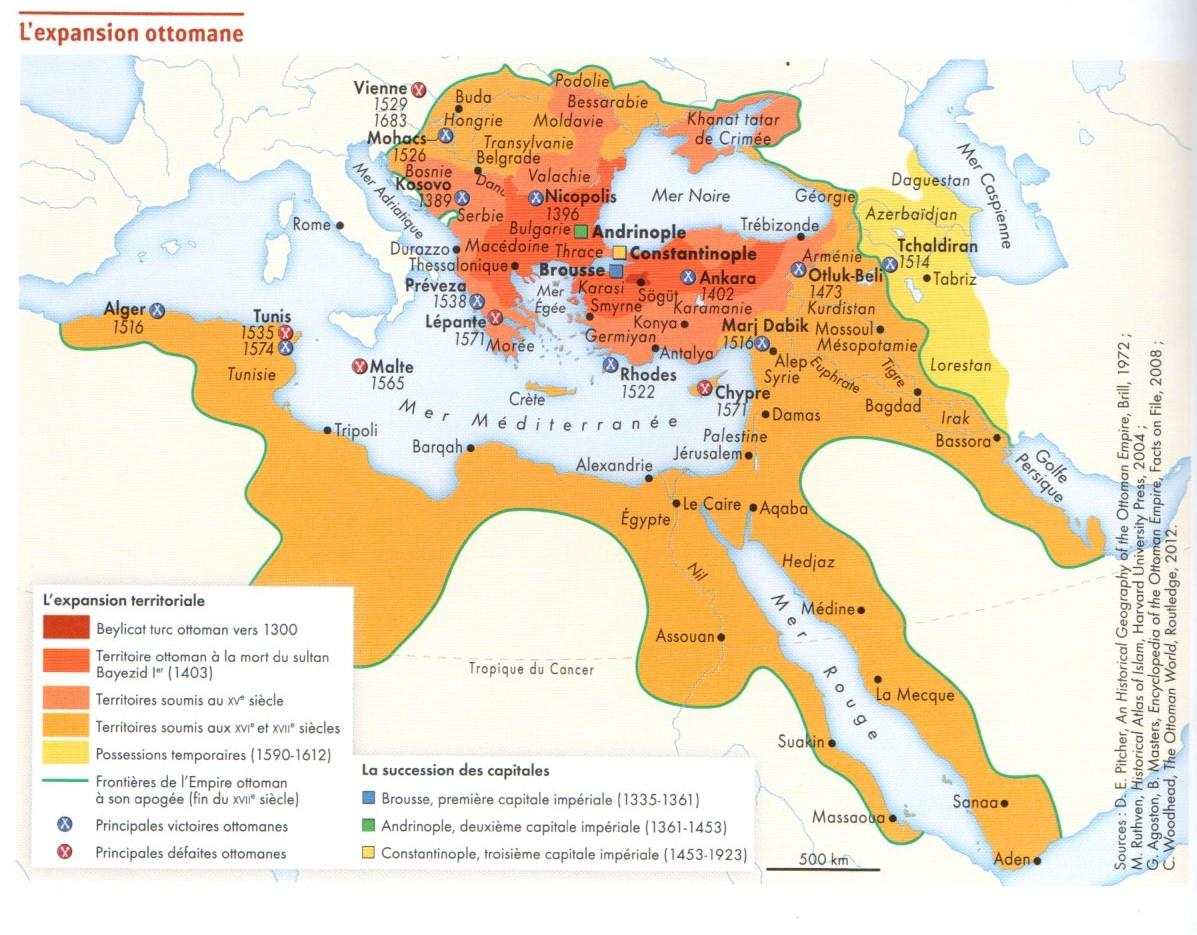
\includegraphics[width=\textwidth]{HistoireIslamMediterranee/Images/EmpireOttoman.png}
\paragraph{Fernand Braudel} s'inspire de Pirenne, mais va travailler sur l'empire des Hasbourg. Il va travailler sur la \Med dans toutes les dimensions : échange, la voir dans son unité. Il travaille avec une question : est-ce qu'il faut inventer le concept, par delà de la \Med espagnole. 

\begin{quote}
    « Dans\sn{Fernand Braudel (dir.), La Méditerranée. L’espace et l’histoire, Paris, Champs Flammarion, 1985,  p. 10} son paysage physique comme dans son paysage humain, la Méditerranée carrefour, la Méditerranée hétéroclite se présente dans nos souvenirs comme une image cohérente, comme un système où tout se mélange et se recompose dans une unité originale. Cette unité évidente, cet être profond de la Méditerranée, comment l’expliquer ? Il faudra s’y efforcer à plusieurs reprises. L’explication, ce n’est pas seulement la nature qui, à cet effet, a beaucoup œuvré ; ce n’est pas seulement l’homme, qui a tout lié ensemble obstinément ; ce sont à la fois les grâces de la nature ou ses malédictions –les unes et les autres nombreuses- et les efforts multiples des hommes, hier comme aujourd’hui. »
\end{quote}

Pour Braudel, la \Med est humaine, physique. Elle est aussi un espace d'échanges commerciaux, linguistiques. Au XIX, période la plus dense d'échanges, avec le bateau à vapeur. 


\paragraph{une \textit{rive} ou \textit{deux rives}}Après lui, les chercheurs vont s'intéresser à la définition même de l'objet : "une seule rive" : greco-romain ? ou des "deux rives", en intégrant l'héritage juif et musulman. La problématique 

\paragraph{Gardet, Berque et Massignon}{Louis Gardet, 1904-1986, philosophe chrétien des théologies comparées, islamologie. Il fonde en 1957 une revue \textit{la revue de la \Med}Il pense la \Med des deux rives, seul moyen de réduire les fractions. \textit{\Med, conception des deux rives } }. et \textit{Jacques Berque}, dépasser la rupture culturelle entre Christianisme et Islam. Islam doit fait le lien entre occident et Afrique / Asie. \textit{Louis Massignon}, Islamologue, mort en 1961, concept de l'\textit{hospitalité}. Il faut accueillir et accueillant de l'autre. Prêtre melchite en secret. Pélerinage en Côte d'Armor des 7 dormants.


\subsection{la mer partagée}

Jean Guilaine, \textit{La \Med partagée}.

La mer, qui est une mer de lien, peut être un obstacle. Avant l'Islam, des ruptures, comme en 395, la rupture entre Empire d'Orient et d'Occident. 

476 : chute de Rome.

1054 : rupture entre Eglise orient et Occident.

1204 : 4ème croisade et pillage de Constantinople.

1453 : conquête de Constantinople. 

Pirenne lui insiste sur l'irruption de l'Islam. 

D'autres insistent sur la peste du VIe siècle qui décime la \Med. 

Après les croisades, les Européens contrôlent les principales villes de la \Med mais ne connaissent pas mieux l'autre. 

\subsection{Les problématiques théologiques} 

\paragraph{Est-ce que Dieu est méditerranéen ?} Non, vue négative de la \Med. Grande mer vers le soleil couchant, mer des philistins, mer Occidentale. La fin du monde. 

\paragraph{Désert} Est-ce qu'on peut dire que le monothéisme est  méditerranéen ? Non, le monothéisme est né dans le désert. Racine sémitique, du désert, entre le Tigre et l'Euphrate.

\paragraph{Au XIIè avant JC, les phéniciens} Les maîtres de la \Med, ce sont les phéniciens qui sont sur la côte occidentale (Gaule, Carthage). La capitale de ce monde, c'est Tyr. Alphabet, art,... Est-ce une première identité mediterannéenne ? 

\paragraph{VIIème siècle : renaissance grecque archaique} \Med, plusieurs mer (Chypre, de Lybie,...). 

\paragraph{Une seule mer au temps des Romains} Avec les Romains, unité de la \Med. Paul va \textit{surfer} sur cette unité de la Mer, après la bataille d'Actium en - 31. La domination est politique mais culturellement, grecque. 

\paragraph{Une fascination de la \Med pour les Dieux} Jérusalem, Damas, 2ème capitale arabe, Rome, Constantinople + Grèce (philosophie grecque).  
\begin{quote}
   Ac 17  : Areopage 
\end{quote}
Dieu des philosophes et Dieu du désert se recontrent et ne forment plus qu'un. L'ouverture de Paul aux Nations. 

\paragraph{Conception de Jésus et la \Med.} Une ouverture à la syro-phénicienne. Jésus sort de la vision "jérusalemo-centrique".

\paragraph{Paul va s'appuyer sur l'Unité politique}
Paul. Unité religieuse de la \Med depuis 313. 3 voyages. 

\paragraph{Les fils du désert devenu des navigateurs, l'Islam} Les bébouins de l'arabie au VII vont devenir des marins. 

\paragraph{acceptation de l'Islam par la Syrie et l'Irak} 639, Syrie très vite islamisé. Pourquoi les chrétiens ont accueilli les arabes : 
\begin{itemize}
    \item peste qui a fragilisé le monde bysantin
    \item proximité culturelle
    \item un monde entre Constantinople et Perse.
    \item Nestorien
\end{itemize}

\paragraph{Apologie} de Jean Damascène 680-708. 675 : petit traité sur l'Islam. 

\paragraph{Empire Sassanide s'effondre} 
641 : l'Egypte capitule
670 : Kerouan
700 : toute l'Afrique est musulmane, plutôt paisible. 


\section{Bibliographie indicative}

\begin{itemize}
    \item     « Chrétiens et musulmans : Quel dialogue aujourd'hui ? », Cahiers de l'Atelier, tome 560, avril-juin 2019.   
    \item    ALBERA Dionigi et PENICAUD Manoël (dir.), Coexistences. Lieux saints partagés en Europe et en Méditerranée, Paris, Musée national de l’Histoire de l’Immigration – Actes sud, 2017.     
    
    \item   ALBERA Dionigi et BERTHELOT Katell (dir.) Dieu, une enquête. Judaïsme, christianisme, islam, ce qui les distingue, ce qui les rapproche, Paris, Flammarion, 2013.     
    
    \item   BERQUE Jacques, Les Arabes, Paris, Actes sud, 1999.     
    \item   BORRMANS Maurice, Prophètes du dialogue islamo-chrétien, Paris, Ed. du cerf, coll. « L’histoire à vif », 2009.     
    \item   CAHEN Claude, Islam, des origines au début de l’Empire ottoman, Paris, Hachette, coll. « Pluriel », 2011. 
    
    \item CAHEN Claude, Orient et Occident au temps des croisades, Paris, Aubier, 2010.     
    
    \item   CAILLEAUX Christophe, « Chrétiens, juifs et musulmans dans l’Espagne médiévale. La convivencia et autres mythes historiographiques », Cahiers de la Méditerranée, n°86, Juin 2013, p. 257-271.     \item   CARPENTIER Jean et LEBRUN François, Histoire de la Méditerranée, Paris, Seuil, coll. « Points Histoire », 2001.     
    \item   CAUCANAS Rémi, Relations islamo-chrétiennes en Méditerranée, entre dialogue et crispation, Presses universitaires de Rennes, 2014.   



    \item   CHEDDADI Abdesselam, Les Arabes et l'appropriation de l'histoire : émergence et premiers développements de l'historiographie musulmane jusqu'au IIe/VIIIe siècle, Paris, Actes sud, 2004.   \item DUFOURCQ Charles-Emmanuel, « La coexistence des chrétiens et des musulmans dans AlAndalus et dans le Maghrib du Xe siècle » In: Actes des congrès de la Société des historiens médiévistes de l'enseignement supérieur public, 9ᵉ congrès, Dijon, 1978, p. 209-224.  
    
    \item GAUDEUL Jean-Marie, Disputes ? Ou rencontres ?, l’islam et le christianisme au fil des siècles, Rome,   \item PISAI, coll. « Studi arabo-islamici », n°12, 1998, 2 volumes.   \item GEORGEON François, VATIN Nicolas et VEINSTEIN Gilles (dir.), Dictionnaire de l’Empire ottoman, Paris, Fayard, 2015.   \item HEYBERGER Bernard, VOGEL Jacob et ASSAN Valérie (dir.), Minorités en Méditerranée au XIXe siècle : Identités, identifications, circulations, Rennes, Presses Universitaires de Rennes, 2019.    \item HORDEN Peregrine and KINOSHITA Sharon (dir.), A Companion to Mediterranean History, Oxford, Wiley-Blackwell, 2014 (cf. Chapitre 34 “Shared Sacred Places”)    \item HOURANI Albert, Histoire des peuples arabes, Paris, Seuil, coll. « Points », 1993.   \item LEJBOWICZ Max (Eds), Les relations culturelles entre chrétiens et musulmans au Moyen Age: Quelles leçons en tirer de nos jours ?, Turnhout, Brepols, coll. « Rencontres médiévales européennes », n°5, 2005.  LOUIS Florian, Atlas historique du Moyen-Orient, Paris, Autrement, 2020.   \item MANTRAN Robert, Histoire de l’Empire ottoman, Paris, Fayard, 1989.   \item PISANI, Emmanuel,  « Le statut du ḏimmī chez al-Ġazālī », MIDÉO [En ligne], 33 | 2018, mis en ligne le 05 juillet 2018, consulté le 28 décembre 2022. URL : 
    \item REYNAERT François, La Grande Histoire du monde arabe, d'Alexandre le Grand à l'islamisme radical, Paris, Fayard, 2015.   \item REYNOLDS, Gabriel Said, The Qurʾan in Conversation with the Bible: Revised Qurʾan Translation of Ali Quli Qaraʾi annotated with Biblical Texts and Commentary by Gabriel Said Reynolds, New Haven, Yale University Press, 2018.   \item REYNOLDS, Gabriel Said, The Emergence of Islam, Minneapolis, MN Fortress Press, 2012.    \item REYNOLDS, Gabriel Said, The Qurʾān and Its Biblical Subtext, London, Routledge, 2010.   \item RODINSON Maxime, Les Arabes, Paris, PUF, coll. « Quadrige », 2002. Histoire des Arabes de 1500 à nos jours Tempus 3 ROGAN Eugene, 2016.   \item SOURDEL Dominique et Janine, 2004.   \item THOMAS History David, ROGGEMA Barbara (eds.) , Leyde  Boston, Brill, 2009 (3 volumes). , Paris, Perrin, coll. « Dictionnaire historique de l’Islam , PUF, coll. », « Quadrige », , ChristianMuslim Relations: a Bibliographical 
\end{itemize}
\chapter{Le statut de dhimmi de la
naissance de l’islam aux Omeyyades}

\mn{Séance 2 (MarieCarmen Smyrnelis) du 24 janvier}


\section{Bibliographie}

\begin{itemize}
    \item CAHEN Claude,
Islam, des origines au début de l’Empire ottoman , Paris, Hachette, coll. « Pluriel », 2011.
    \item 
GAUDEUL
Jean Marie, Disputes ? Ou rencontres ?, l’islam et le christianisme au fil des siècles, Rome,
PISAI, coll. « Studi arabo islamici », n 12, 1998, 2 volumes.
    \item 
HOURANI Albert,
Histoire des peuples arabes , Paris, Seuil, coll. « Points », 1993.
    \item 
LEWIS Bernard,
Les Arabes dans l’histoire , Paris, Flammarion, « Champs », 1993.
    \item 
RODINSON Maxime,
Les Arabes, Paris, PUF, coll. « Quadrige », 2002.
\end{itemize}


\section{Les débuts de l’islam}

\subsection{la péninsule arabique à la veille de l'apparition de l'islam}

\paragraph{une lutte entre l'empire bysantin et l'empire sassanide}
\begin{Def}[Empire]
Ce qui caractérise l'empire, c'est l'hétérogéneité des peuples qui la compose. 
\end{Def}

 \subsection{Repères chronologiques}
 \begin{itemize}
   \item	570-580 : naissance de Mahomet à La Mecque
\item 	622 : installation à Médine (Hégire)
\item 628 : pèlerinage annuel à la Mecque négocié avec les autorités.
\item 	630 : conquête de La Mecque
\item 	632 : mort de Mahomet
 \end{itemize}

\begin{figure}[h!]
    \centering
        \sidecaption{lorian Louis, Atlas historique du Moyen-Orient, Paris, Autrement, 2020, p. 33}
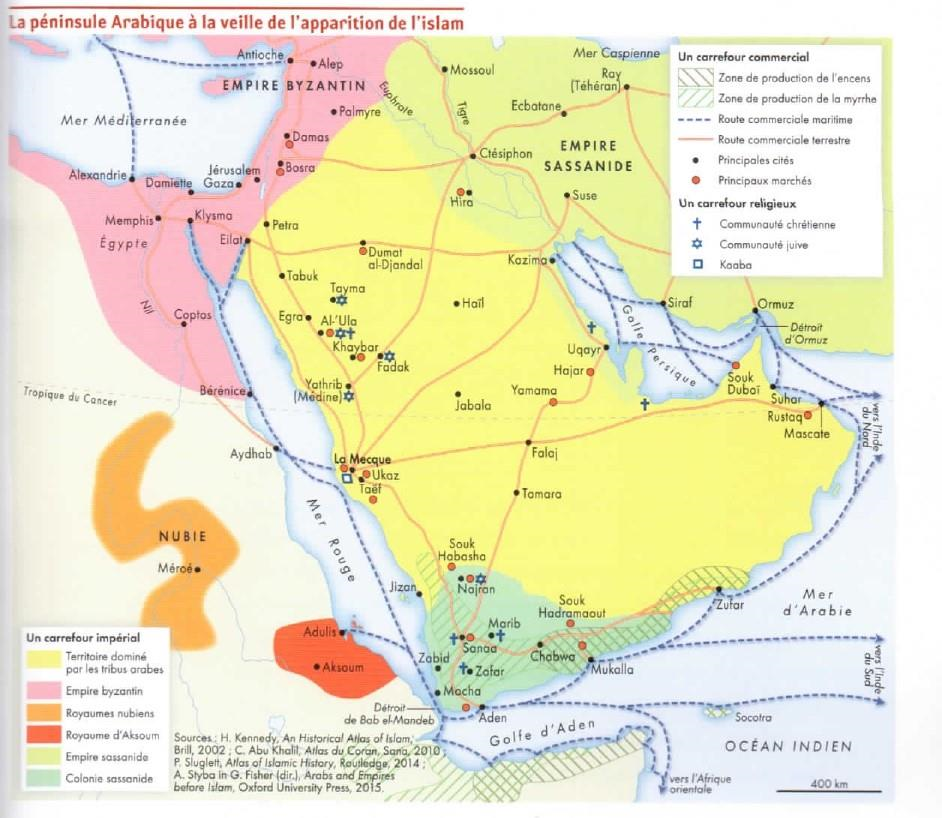
\includegraphics[width=\textwidth]{HistoireIslamMediterranee/Images/PeninsuleArabe.png}

    \label{fig:my_label}
\end{figure}


\paragraph{ce qu'en disent les historiens} A Médine, il part probablement à la demande des Médinois, s'impose pour son jugement. Fonde l'\textit{umma}. 

\paragraph{Juxtaposition de l'Umma avec les tribus} chaque tribu garde ces droits mais face à Mohammed, on suit la loi.

\paragraph{Première "constitution" médinoise} relation des membres entre eux, comment on traite en dehors de l'\textit{umma}. 
La foi va remplacer le lien de sang, nouveau lien. La source de l'autorité passe de la vue publique à Dieu.

\paragraph{L'umma prend une dimension de l'umma} Mohammed fonde à la fois une foi mais aussi un corps politique. 
\begin{Def}[théocratie]
    mélange politique et religieux
\end{Def}
Mais on plaque la politique actuelle alors que c'est une réalité bien différente.

\paragraph{de l'attaque des caravanes à l'extension du territoire} 

\paragraph{630 - Mecque : des affaires politiques avec les tribus} mais pas religieux qui reste quelque chose d'individuel dans un premier temps.  \textsc{Une vraie question pour la suite du collectif et de l'individuel et en particulier pour la conversion. }
Au début, la tribu accepte de ne pas attaquer les musulmans, elle accepte de payer l'impôt religieux mais elle n'est pas obligée de se convertir.

L'accord se place toujours avec Mahomet jusqu'à sa mort.

\paragraph{632 mort de Mahomet} les difficultés commencent.  Il n'avait pas laissé d'instructions de succession. 


\section{Les Rasidun les « bien guidés », successeurs de Mahomet et califes}

 

\paragraph{de nombreuses questions à la mort du Prophète} Qui va avoir l'autorité ? Comment gérer le statut des non musulmans ? pratique du Coran

\paragraph{Alors que ce monde connaît un bouleversement politique} Avec un embryon étatique. Certains historiens considèrent l'empire arabe à la mort de Mahomet.


\paragraph{les Rasidun (632-661) : successeurs de Mahomet}
\begin{itemize}
  \item 	Abu Bakr (632-634)\sn{beau-Père de Mahommed, déput de l'institution du califat}
\item 	Umar (634-644)
\item 	Uthman (644-656)
\item 	Ali (656-661)
\item 	les Omeyyades (661-749) => transfert de la capitale à Damas
\end{itemize}

\paragraph{Abu Bakr} Chef d'une communauté et chef d'un territoire. Pas trop de difficultés du fait de la durée de deux ans

\paragraph{Umar} Cela se complique. Est tué par un esclave persan. comprend la question Islam et Arabie, alors que l'Islam rentre en Perse.  

\paragraph{Des révoltes} de tribus s'opposant au choix d'Abu Bakr et Uman. Pour calmer ces tribus, l'extension du territoire est nécessaire.

\paragraph{Question de l'Empire} avec la taille du territoire, se passe la question de l'acceptation culturelle et religieuse locale.
\begin{itemize}
    \item \item 	633-637 : conquête de la Syrie
\item 	639-642 : conquête de l’Egypte. Se passe bien du fait que les coptes en ont assez de Byzance. Du côté de Byzance, on a une armée de mercernaires peu motivés d'appliquer une loi peu acceptée par les populations locales. 
\item 	634-652 : conquête de la Perse. 

\end{itemize}

\paragraph{utilisation du désert} pour se retirer et communiquer. Installation des villes à la frontière du désert, villes d'appui, où les arabes sont majoritaires. Dans ces villes, \textit{amsar}, l'arabe est la langue. Dans le reste, les musulmans sont minoritaires.   
C'est assez classique dans un empire, où la culture de l'empire est minoritaire.

\begin{Ex}[Fustat]
Ils quittent Alexandrie et fondent Fustat.  Ces villes nouvelles, \textit{amsar}, sont encouragées par des taxes. C'est une expansion \textit{arabe} et pas forcément de l'Islam, puisque les tribus arabes ne sont pas toutes islamisées.
\end{Ex}

\begin{Ex}[Bosra en Syrie]
\begin{marginfigure}
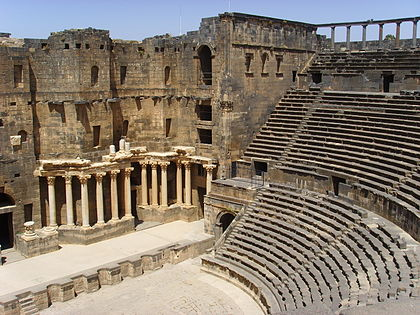
\includegraphics[width=\textwidth]{HistoireIslamMediterranee/Images/TheaterBosra2.jpg}
\end{marginfigure}
    Avait déjà une population arabe importante avant la conquête. 
\end{Ex}

\paragraph{Respect des cultures locales} D'abord, on préserve les cultures locales. L'idée d'une conversion totale ne se pose pas, en dehors de l'Arabie. On demande la soumission et en échange, on a la protection. 

\paragraph{Propriété respectée} sauf si propriété d'un disparu ou propriété de l'Etat. Mais uniquement au début. 

\paragraph{Un impôt de soumission} Il est interdit quand on n'est pas arabe, de s'habiller comme un arabe. 
\begin{Def}[mawali]
    ce sont des non arabes convertis, normalement égaux, ne payent pas de taxes mais considérés comme socialement inférieurs.
\end{Def}


\paragraph{Uthman} Arrêt de la conquête. Se pose le problème de l'organisation. 

\paragraph{de fortes révoltes}ne vise pas directement Uthman, elles ne sont pas non plus religieuses mais liés à des enjeux de pouvoir. Uthman avait moins de légitimité et apparaît faible.
Les nomades se révoltent depuis l'Egypte et depuis Médine contre les hommes de la Mecque.  

\begin{Prop}
A cette époque la relation et la fidélité sont toujours individuels au calife. 
\end{Prop}

\paragraph{L'assassinat de Uthman } par un esclave perse. Sans doute pour un problème politique. Annonce pour certains historiens la lutte de la Perse.


\paragraph{Ali} proclamé Calife à Médine. Pour des raisons politiques, il démet les fonctionnaires nommés par Uthman mais il ne punit pas les meurtriers de Uthman. Il est donc accusé d'avoir une responsabilité dans sa mort.

\paragraph{Bataille de Bassora} Ali la gagne mais sort affaibli. Le gouverneur de la Syrie, pour venger Uthman, lève une armée et attaque Ali. 

\paragraph{} Le gouverneur de Syrie met le coran sur les lances. Ali est tué et son fils renonce au califat. Le gouverneur de Syrie devient Calife Omeyyade.

 


\section{La dynastie des Omeyyades}


\paragraph{le Calife  Muʿāwiyah ibn ʾAbī Sufyān} crée la dynastie. Centraliser le pouvoir. 

\paragraph{transfert de la capitale de Médine à Damas} On s'éloigne de l'Arabie. L'influence des arabes en Syrie devient très importante. On contrôle la \Med orientale. Même si les Omeyyades restent attachés au désert \mn{cf qsars, château dans le désert}.

\paragraph{La \textit{chura}} Muʿāwiyah crée un conseil consultatif et executif, le conseil des tribus. Il s'appuie sur des instances qu'il créé. Via les gouverneurs et la \textit{chura}, il gouverne sur la totalité du territoire.

\paragraph{Le personnel de l'empire byzantin ou perse reste} 



\begin{figure}[h!]
    \centering
      \sidecaption{\textsc{De Muhammed aux Omeyyades : expansion et division de l'Islam}. Florian Louis, Atlas historique du Moyen-Orient, Paris, Autrement, 2020, p. 37.
      Certaines batailles vont avoir un rôle important dans le positionnement de l'Islam}
   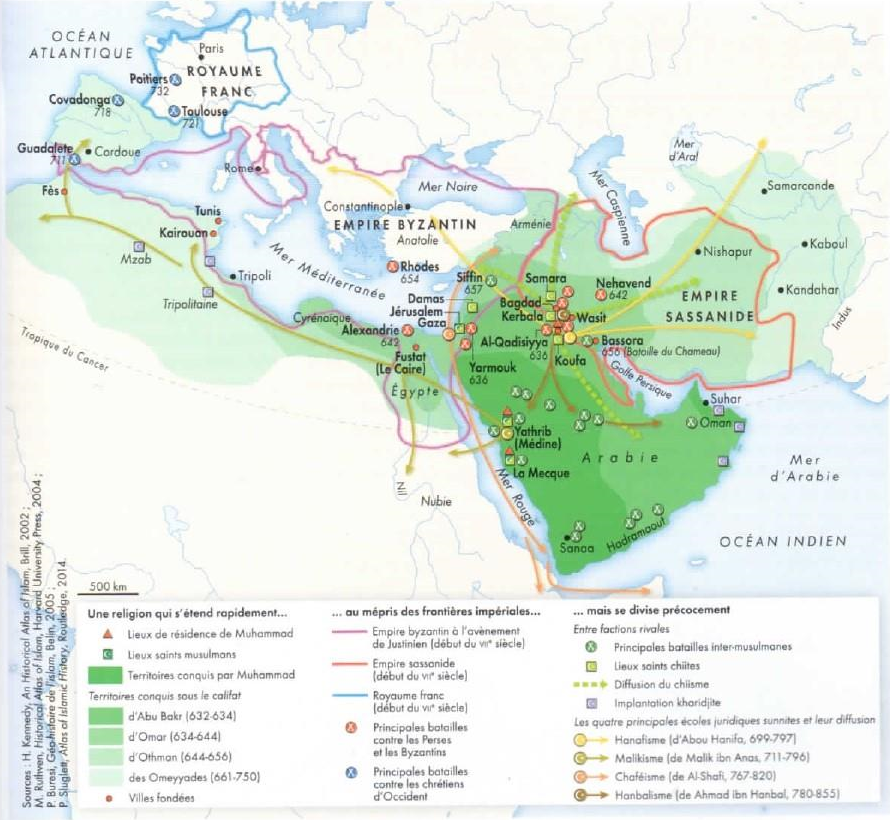
\includegraphics[width=\textwidth]{HistoireIslamMediterranee/Images/ExpansionMusulmane.png}
  
    \label{fig:my_label}
\end{figure}
\paragraph{Principales conquêtes}
\begin{itemize}
   \item 	696 : Chute de Carthage
\item 	710 : débarquement en Espagne, par le soutien des tribus berbères
\item 	732 : bataille dite de Poitiers (Omeyyades mis en échec par Charles Martel)
\end{itemize}
Ils vont essayer de prendre Byzance à deux reprises, échec.

\paragraph{Son successeur,Yazīd Ier} avec des dissensions importantes. Développement d'une civilisation brillante. Une minorité d'arabe dirigeant une majorité non musulmane.

\paragraph{des conversions pour des raisons diverses} Cela peut être pour s'intégrer dans l'élite, la simplicité de l'Islam avec des modalités simples, pour des raisons fiscales. Les zoroastriens se convertissent plus facilement que les chrétiens. 
A partir d'un certain moment, pour des raisons économiques, les Omeyyades découragent les conversions. 

\paragraph{Les partisans d'Ali} Les \textit{Mawalis} qui se sont convertis mais ne dépendant pas d'une tribu arabe (berbere, persans, Iraniens,...), surtout dans les \textit{amsar}. Ils ont une paie inférieure,... Leur poids démographique augmente. Ils vont trouver une traduction religieuse dans le Chi'isme : ils manifestent d'une façon politique contre le pouvoir établi. Ce ne sont pas uniquement des non arabes qui sont chiites. \textit{Une complexité} avec des mariages mixtes (avec esclaves). La révolte boue. 
Ce n'est donc pas qu'une révolte religieuse mais sociale et politique. Les "demi-arabes" vont se révolter et soutenir \textit{Ali} et ses descendants. 

\paragraph{Consolidation du pouvoir} Monnaie (Dihram et Dinar)... 


\section{Le statut de dhimmi}

\begin{Def}[dhimmi]
    Engagement, notion de pacte.
\end{Def}

\paragraph{Que fait-on des non-musulmans ?} D'abord, en tant qu'Empire, il y a déjà des échanges, avec des chrétiens et des juifs. On a besoin d'eux pour le commerce. Il y a aussi la place des chrétiens dans l'administration. Tous ces contacts vont commencer dès Mahomet.

 Mahomet \sn{Godel} rencontre en 632 une tribu chrétienne au Yémen (Najraf). 

 \paragraph{629 Attaque d'une oasis d'une tribu juive} Puis une tribu chrétienne. Pour les \textit{religions du livre}, protection et paiement de l'impôt (\textit{jizya}, impôt par capitation et \textit{kharadj} impôt collectif, somme forfaitaire par communauté). Pour les autres religions, conversion ou mort.

 \paragraph{Les \textit{harbi}} les musulmans rencontrent les \textit{harbi} Le terme harbi, sert à désigner un non-musulman vivant en territoire non-musulman. Mot originaire d'une région du dar al-harb qui était connue particulièrement hostile à la jeune communauté musulmane.

\paragraph{statut de Dhimmis} Impôt, 
 pas d'arme, pas de nouveau culte, habit différent, leur témoignage n'est pas recevable devant les tribunaux. 
 Et pourtant, une acceptation des arabes plutôt que les byzantins. 

 \paragraph{des lieux de culte} des partages temporaires : on peut décider de partager à certaines heures l'Eglise aux arabes, tout au début de l'Islam et le temps que l'on crée une mosquée.


 \paragraph{Pourquoi ne parle-t-on pas plus des dhimmis dans ce cours} Tout simplement parce qu'on a peu d'informations sur les \textit{dhimmis} à cette époque. 

 \paragraph{Le grand père de Jean Damascène} négocie la reddition de Damas. Avant de devenir moine, Jean était fonctionnaire. 734 : démission de Jean Damascène dans un contexte plus difficile. 
 Sous Umar (?), les chrétiens vont être exclus de l'administration.

 \paragraph{Un statut jusqu'en 1923}



 \section{Histoire}

 \mn{CHarbel Attallah 30/1/23}

 \paragraph{une décade des califes bien guidés} La conquête de la grande Syrie (Irak, Syrie, Liban,...) s'est faite à l'époque de Umar de façon aisée. 


 \paragraph{Un des premiers pactes} Jizya à payer. Entre Umar et le patriarche de Jérusalem de l'époque. 

 \begin{Def}[jizya]
     Impôt permettant de restant vivant sur le territoire et permettant de pratiquer sa religion.
 \end{Def}

\paragraph{une seule référence Coranique} verset médinois. Muhammed va rencontrer les chrétiens à Médine, les \textit{najar}. D'où le caractère polémique et parfois violent dans les versets médinois. 
 \begin{quote}
    Combattez également ceux parmi les gens du Livre qui ne professent pas la religion de la vérité, à moins qu'ils ne versent la \textit{jyzia } directement et en toute humilité.
     Co 9, 29
 \end{quote}

 Le statut de \textit{dhimmi} a donc été pensé, à \textit{Médine.}

 \subsection{Les grands historiens arabes}

 \paragraph{At-Tabari} (839-923) \textit{Tarikh ar-Rusul w-lmuluk} histoire des envoyés de Dieu et des Rois

 \paragraph{Ibn 'Assakir} (1106-1176) Tarikh Dimashq (Histoire de Damas), 80 volumes. 


\paragraph{La capitulation de Jérusalem} At Tabari rapporte Umar et Sophronius. 
 637 (an 15) : 
 
 \begin{quote}
     Au nom de Dieu, Clément et Miséricordieux.

Voici ce que garantit le Serviteur de Dieu, `Umar, Commandeur des Croyants, aux habitants d’Aelia [1] en terme de sécurité. Il leur garantit la sécurité de leurs personnes, de leurs biens, de leurs églises et de leurs croix, lcelles-ci étant en bon ou mauvais état, ainsi qu’à toute leur communauté. Leurs églises ne seront ni investies en état d'habitation ni détruites. Rien ne leur sera ôté, ni à leurs propriétés ni à leurs croix ni à leurs biens. Ils ne seront pas convertis malgré eux et nul d’entre eux ne sera opprimé. [Ne résidera aucun Juif avec eux à Aelia.] Les habitants d’Aelia devront s’acquitter de la capitation comme les habitants des autres villes. Quiconque d’entre eux partira aura la garantie de la sécurité de sa personne et de ses biens jusqu’à ce qu’il parvienne à sa destination. Quiconque d’entre eux restera à Aelia [1] sera en sécurité et il devra, comme les habitants d’Aelia [1], s’acquitter de la capitation. Ceux, parmi les habitants d’Aelia [1], qui désirent rejoindre les Byzantins avec leurs biens, abandonnant leurs églises et leurs croix, auront la garantie de la sécurité de leur personne, de leurs églises et de leurs croix, jusqu’à ce qu’ils parviennent à leur destination.

Quiconque, parmi les habitants de la terre, habitait dans la ville avant le meurtre d’untel, pourra, s’il le souhaite, y demeurer, et devra, comme les habitants d’Aelia [1], s’acquitter de la capitation. S’il le souhaite, il pourra rejoindre les Byzantins. S’il le souhaite, il pourra retourner chez les siens. Aucune capitation ne sera prélevée avant la récolte.

Le contenu de cet écrit en ce qu’il stipule du Pacte de Dieu, de la protection (dhimmah) de Son Messager, de la protection des Califes et de la protection des Croyants sera intégralement appliqué s’ils s’acquittent de la capitation. [2]

Sont témoins Khâlid Ibn Al-Walîd, `Amr Ibn Al-`Âs, `Abd Ar-Rahmân Ibn `Awf et Mu`âwiyah Ibn Abî Sufyân. Ecrit et entré en vigueur en l’an 15. »
 \end{quote}


 \paragraph{Ibn Arabi : radicalisation de la dhimmi} Ibn Arabi (Espagne, Andalousie, avec des rois catholiques qui essayent de reconquérir l'Espagne) rapport cette capitulation d'Omar : 

 \mn{ Paradigme de l'autocentralité foncière

 comment je peux avoir une si profonde mystique et je peux rester aussi exclusiviste.}


\begin{quote}
 Ils [les chrétiens] ne chevaucheront pas sur la selle, ils ne porteront pas d'épée à la ceinture, et ils ne posséderont pas d'autre genre d'armes; ils n'utiliseront pas les lettres arabes dans leurs sceaux, et ils ne vendront pas de boisson alcoolisées; ils couperont la partie antérieure de leur chevelure (sur le front), ils garderont partout leur façon de s'habiller, et ils portefront aussi une ceinture (\textit{zunnâr}) autour de la taille.
 
 Ils n'exhiberont ni leur croix ni leur livres dans les rues parcourues par les musulmans; ils n'enterreront pas leurs morts à côté des morts musulmans, ils ne feront sonner leurs cloches que très doucement, ils n'élèveront pas la voix en lisant dans leurs églises, qui sont proches des musulmans.
 Ils ne feront pas de tours [en procession], ils n'élèveront pas la voix en accompagnant leurs morts [aux funérailles] et ils n'allumeront pas de feu [des bougies] en faisant cela. Il n'achèteront pas les esclaves qui ont étés destinés aux musulmans.

 Au cas où ils transgresseront une quelconque de ces capitulations (\textit{shurût}) qui leur sont imposées, ils n'uaront plus de droit de protection (\textit{dhimma}) et dans ce cas-là, il sera licite aux musulmans de les traiter comme des gens rebelles et séditieux

 \end{quote}
On voit bien le caractère beaucoup plus restrictif de ce statut.
 Est ce écrit par Umar ?  C'est un texte de Umar II, 5ème calife Omeyyade.

 Les soufis renvoient facilement leurs textes aux califes bien guidées pour donner un \textit{statut d'infaillabilité}. 

 \paragraph{Quelle anthropologie sous-jacente ?} Face à la beauté des villes (Damas, Alexandrie,...), les musulmans vont garder l'administration. En particulier, le grand père de Jean Damascène qui reste focntionnaire.

 
\include{HistoireIslamMediterranee/3.JeanDamascène.tex}
\chapter{Les relations islamo-chrétiennes sous les Abbassides}

\section{Bibliographie}

\begin{itemize}
    \item 
CAHEN Claude,
Islam, des origines au début de l’Empire ottoman , Paris,
Hachette, coll. « Pluriel », 2011.
    \item 
HOURANI Albert,
Histoire des peuples arabes , Paris, Seuil, coll. « Points »,
1993.
    \item 
LEWIS Bernard,
Les Arabes dans l’histoire , Paris, Flammarion, « Champs »,
1993.
    \item 
RODINSON Maxime,
Les Arabes, Paris, PUF, coll. « Quadrige », 2002.
 
    \item \textbf{John Tolan}, spécialiste des \textit{Dhimmis} au Moyen-âge.
Par ce programme de recherche, a permis d'avancer sur le sujet.
\end{itemize}


\section{Les Empires musulmans : la umma éclatée}

\begin{figure}
    \centering
    \sidecaption{Florian Louis,
Atlas historique du
Moyen Orient , Paris, Autrement,
2020, p. 39.}
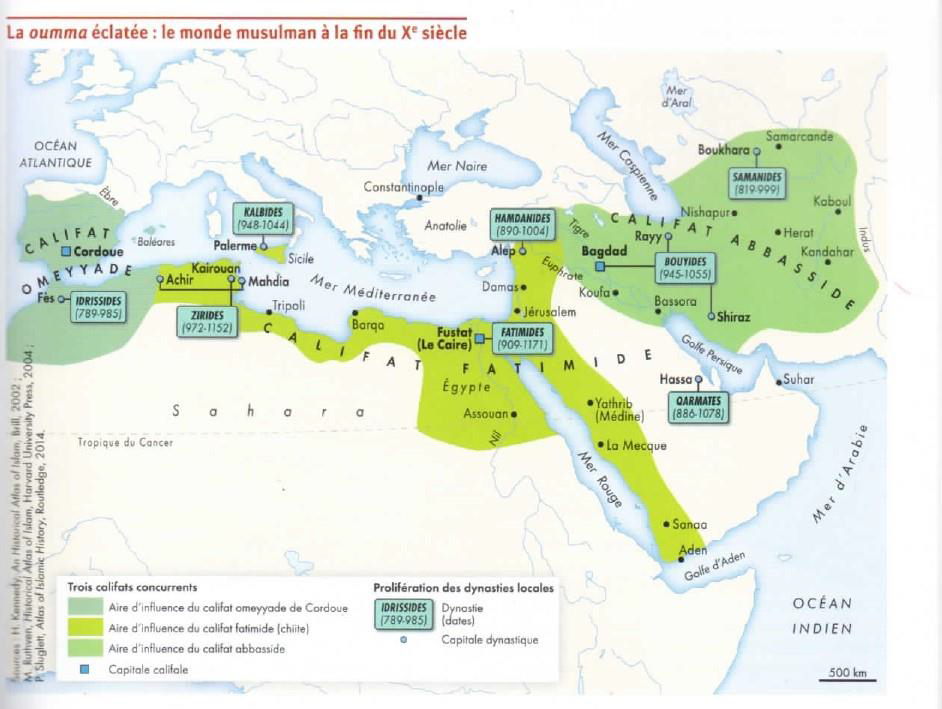
\includegraphics[width=0.8\textwidth]{HistoireIslamMediterranee/Images/SunnismeEclateX.png}
    \label{fig:my_label}
\end{figure}

\paragraph{Pourquoi un changement de régime} d'abord des raisons militaires avec des défaites (750)= face aux abbassides, mais aussi des mécontentements contre les Ommeyyades (les \textit{mawalis}, forte opposition). 

Diverses interprétations : 
\begin{itemize}
\item les orientalistes disent que c'est une opposition entre persans et arabes.
    \item Bernard Lewis : difficile d'accepter la position des orientalistes car ils projettent leurs visions nationalistes du XIXe.
    \item dimension religieuse. en particulier insiste Claude Cahin : plus du chisme religieux que Bernard Lewis. 
\end{itemize}

\begin{Synthesis}
Au dela des raisons militaires, il n'y a pas consensus sur les raisons, religieuses ou oppositions entre mawalis et arabes.
\end{Synthesis}

\paragraph{750 : début de l'empire abbasside} Transfert de la capitale à Bagdad. Ville carrefour commercial permettant de relier via l'intérieur des terres \Med à l'Inde : importance de la mésopotamie. \mn{repères chronologiques : 

Apogée de l’Empire abbasside sous le règne d’
Harun al Rachid (786
809)
 
Apogée de la puissance des Omeyyades en Espagne sous le règne du
calife Abd al Rahman III (912 961) => califat omeyyade en Espagne à
partir du Xe siècle
 
Création de la dynastie fatimide en Tunisie à partir de 910 puis
occupation de l’Egypte en 956 => califat fatimide}

\paragraph{Transformation des modes de succession} Mécontentement de la succession califaire qui serait dynastique : comment intégrer mawalis, esclaves ?...


\paragraph{Une organisation avec une bureaucratie reprise sur le monde perse} ministère, les \textit{diwans} : chancellerie. Des fonctionnaires pour faire tourner la bureaucratie. Des forces armées aussi organisées.  Comme tout empire, découpage de l'espace en province avec un gouverneur, l'\textit{émir}. Et pour la partie financière, l'\textit{amil}\sn{Les Abbassides reprennent les traditions administratives des sassanides. L’administration centrale est formée de bureaux ou offices (diwan) tenus par un corps de secrétaires (kuttab) : le bureau de l’impôt foncier (diwan al kharâdj), le bureau des domaines (diwan al diya), le bureau du Trésor (bayt al Mal), le bureau de la chancellerie (diwan al rasail), le bureau de l’armée (diwan al djaish). La poste (barid) a un rôle très important de communication et de renseignement. Les provinces sont dirigées par des gouverneurs (Khatib, puis émir et wali). Au début de l’Empire, leur gouvernement est souvent de courte durée car ils sont tentés de s’enrichir très vite et sont dénoncés par les hommes de la poste. Les finances des provinces sont confiées à un directeur des impôts (amil), la justice dépend du cadi. }. L'idée est toujours de favoriser le lien entre local et central. Le renseignement est aussi mis en place, pour anticiper les révoltes. 

\paragraph{Emergence de nouvelles classes sociales} mieux rémunérés. L'Empire est riche économiquement. Canne à sucre, blé, or, fer,... Grâce à ces ressources, va pouvoir se développer.

\paragraph{de grands travaux d'irrigation} en reprenant et développant les techniques d'irrigation grecques. 

\paragraph{Une imposition forte} le Kharadj, la capitation pour les non-musulmans. D'où la fonction d'\textit{Amil} avec ses représentants locaux.

\paragraph{le Qadi, fonction de jugement religieux} séparé de l'émir.



\paragraph{un siècle de rayonnement} sous le règne d'Harun al-Rachid (786-809). A sa mort, on voit déjà des signes de fragilisation avec guerre fratricide entre ses enfants. 


\paragraph{Après Harun, des princes autonomes}  830 : Sicile, leur permet de monter en Italie. 

\paragraph{Al Andalous} en 756, deuxième étape de la prise de l'Espagne (première installation en 710, les Omeyyades en Espagne). Pourquoi ce deuxième prise ? Les Omeyyades chassés de Damas vont s'installer en Espagne et chasser les berbères qui contrôlaient l'Espagne. Jusqu'en 1331. D'abord avec le titre d'Emir : il ne veut pas rompre l'\textit{umma}. Mais après le X, il prend le titre de \textit{calife d'Espagne}. 

\paragraph{Le califat Fatimide } Au meme moment, il y a eu une autre dynastie, en Tunisie en 910, d'origine Chiite, qui va se proclamer calife (qui donnera le califat fatimide). Pour des raisons religieuses et politiques (ils ne veulent pas être un pouvoir local), ils vont en Egypte (956) et fondent le califat fatimide.   Ils vont calquer leur organisation sur le califat abbasside (viennent de la péninsule arabique, chiite, descendants d'Ali et Fatima). Ils ne vont pas imposer leur doctrine aux musulmans egyptiens qui vont rester sunnites.  Une vraie question de la raison de cette non-imposition de la foi chiite.

\paragraph{Revenons à l'Espagne} une cour, avec des esclaves venant de la mer noire. Une armée composite, développement des villes, agriculture de subsistance (avec les berbères), administration calquée sur les abbassides. Cour de savants, musiciens. Jusqu'au X. Eclate en \textit{Taifas}, petites principautés et dynasties locales. 

\paragraph{Indépendance du Maroc par rapport à l'Espagne Omeyyade} Fès. Avec les Idrissides. 






%\includegraphics{}
% -------------------------------------------------------------------------------------------------
\section{Des relations islamo-chrétiennes de nature diversifiée}
% -------------------------------------------------------------------------------------------------

\paragraph{division religieuse} D'un côté il n'y a pas de pression pour se convertir mais la seule division qui va rester, et qui va être légalisé, c'est la distinction musulman / non-musulman. 


% -------------------------------------------------------------------------------------------------
\subsection{Au coeur de l'Empire des Abbassides}

\paragraph{un monde où l'islam est prépondérant} caravansérail, développement de l'arabe,... Le temps scandé par les 5 appels à la prière, ramadan, calendrier musulman.  \sn{A la différence de l'Empire Ottoman, qui est aussi scandé par les temps juifs et chrétiens}. D'un règne à un autre, d'une région à l'autre, il peut y avoir des changements.

\paragraph{Distinction des Dhimmis} reste le même. Le statut implique protection. Cela ne sera pas toujours le cas. 

\paragraph{Asymétrie} Remi Brague insiste sur la relation d'asymétrie.  Des différences religieuses, des différences d'habits,... Il ne faut pas trop idéaliser le statut de minorité en monde musulman : infériorité.
Pendant les fêtes religieuses chrétiennes et juives, il y a souvent des débordements. 
\begin{Ex}
Riche marchand chrétien. 
\end{Ex}

Mais à remettre dans un contexte où il y a aussi intolérance vis à vis des Chiites, riches marchants musulmans au sein du monde musulman,  Il ne faut pas idéaliser. Le Kharaj, impôt foncier, est plus élevé pour les non musulmans, les habits avec des couleurs différentes, des rites autorisés, interdiction d'avoir une maison plus élevée qu'un musulman, monter à cheval...

\paragraph{place des musulmans}
VIII : Moins de 10\% de musulmans, plutôt modeste. A la fin du X, la grande partie de l'empire est devenue musulmane : échapper au statut du dhimmi. Rigidification du statut inférieur. Il n'y pas de politique de conversion à l'Islam mais on ne peut revenir à sa religion d'origine.  

\paragraph{des quartiers par communauté} On soupçonne que cela commence aux époques des abbassides. Limite des échanges. Et du division du travail. Reste à creuser le développement économie et commercial de l'empire Abbasside. Des échanges jusqu'en Chine, Byzance, Scandinavie,...
Par rapport à ce qui dit Pirenne de la séparation de la méditerranée, ce n'est pas tout à fait juste. Les juifs comme intermédiaires.
Les banquiers sont essentiellement chrétiens et juifs (mais des musulmans banquiers existent).


\paragraph{Langue arabe} L'arabe, langue de l'administration, juridique, littérature... A coté des autres langues qu'on parle dans l'Empire abbasside. Arabisation via l'administration et en même temps, interaction qui existe entre les différents monothéismes. 

\paragraph{Révolte} entre arabes et coptes contre le gouverneur.  Où ? Caire ? 





% -------------------------------------------------------------------------------------------------
\section{En terre chrétienne conquise}
\begin{figure}
    \centering
    \sidecaption{Florian Louis,
Atlas historique du
Moyen Orient , Paris, Autrement,
2020, p. 38.}
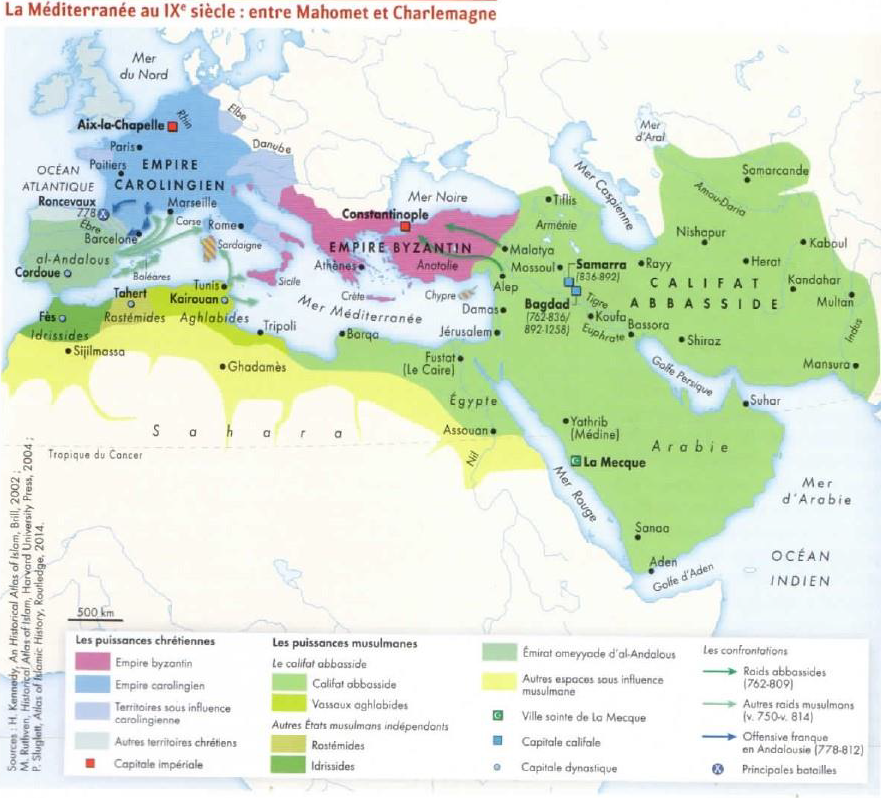
\includegraphics[width=0.8\textwidth]{HistoireIslamMediterranee/Images/MedIXe.png}
    \label{fig:my_label}
\end{figure}

 
\subsection{La Convivencia Espagnole}
\paragraph{la Convivencia} Espagnole. Mythe d'Al Andalus. Contrôle d'un pays essentiellement chrétien par des musulmans + berbere + esclave. Le statut de Dhimmi s'applique : 
\begin{itemize}
    \item pas de nouvelles eglises ni monastère
    \item pas de croix sur les Eglises, pas de cloche
    \item pas de procession
    \item pas de prière ostentatoire
    \item interdit vestimentaire, pas d'arme
\end{itemize}

John Tolan a montré que dans la pratique, quelques églises créées.

\paragraph{la cathédrale de Cordoue} partagée par les Chrétiens et les musulmans. l'Emir va acheter l'Eglise et va les autoriser à créer une nouvelle Eglise. 

\paragraph{fin X} majorité arabophone et musulmane. Raison : 
\begin{itemize}
    \item Attirance ? religieuse ? ou pas assez de prêtres ou Evèques ? face à ce vide, on se tournerait vers les musulmans
    \item échapper aux taxes
    \item statut privilégié. 
\end{itemize}


\paragraph{C'est trop pour le chrétien Alvaro ! Milieu du IXè}
\begin{quote}
    «
Beaucoup\sn{Cité par Bernard Lewis,
Les Arabes dans l’histoire , Paris, Flammarion, « Champs », 1993, p. 153.} de mes coreligionnaires lisent la poésie et les contes des Arabes ; ils
étudient les écrits des théologiens et des philosophes mahométans, non pour les
réfuter, mais pour apprendre comment s’exprimer eux mêmes en arabe avec une
correction et une élégance plus grandes. Où trouver aujourd’hui un laïc qui lise les
commentaires en latin sur les Saintes Ecritures ? Qui, parmi eux, étudie les Evangiles,
les Prophètes, les Apôtres ? Tous les jeunes chrétiens connus pour leurs talents ne
connaissent que la langue et la littérature des Arabes ; ils lisent et étudient avec zèle
les livres arabes, constituant à grands frais d’énormes bibliothèques et proclamant
partout, à qui veut les entendre, que cette littérature est digne d’admiration. Parmi des
milliers d’entre nous, à peine en trouve t on un qui sache écrire une lettre à un ami en
un latin passable, mais innombrables sont ceux qui peuvent s’exprimer en arabe et
composer de la poésie en cette langue, avec plus d’art que les Arabes eux mêmes. » 
\end{quote}

Pas le même statut entre Tolède, Seville et Cordoue, les autorités musulmanes entretiennent de bonnes relations vis à vis des autorités religieuses. Les Évêques sont validés par les Emirs. Que signifie la présence d'un Évêque à la cour ? 

\paragraph{la ville de Tolède} Arabisé mais restée chrétienne.  L'époque des Omeyyades et Taifas : ok convivencia mais après, ce n'est plus du tout le cas (Almoravides puis les Almohades, très rigoristes).

\paragraph{John Tolan : ne plus utiliser le terme de convivencia et aller au delà} Les Mozarabes, chrétiens arabisants. D'après les textes juridiques, charte urbaine (indiquant l'interdiction de fréquenter l'autre), cela veut dire que la pratique existe. L'image doit être nuancée. Modèle de cosmopolitisme / convivencia, est repris dans des unités politiques (dialogue Israel / Palestine, Chypre,...) : on va revenir sur cet âge d'or. 


\paragraph{vit on côte à côte} Il ne semble pas y avoir des quartiers spécifiques. Longue durée de la vie. Relation amicale avec quelqu'un d'une autre religion : dangereux pour les \textit{muftis} : interdiction des fêtes chrétiennes. Au même moment, le calife participe à une course équestre chrétienne. 
John Tolan : on ne fait pas appel à une nourrice juive ou chrétienne, on n'achète pas de la viande au boucher chrétien. Mariage mixte réglementé. On peut avoir des esclaves chrétiens.


\paragraph{Au quotidien vs texte législatif} Un \textit{Dhimmi} ne doit jamais avoir de pouvoir sur le musulman. Mais dans la pratique ? Attention, John Tolan travaille surtout sur la période post-abbasside. 

\paragraph{Tolède Chrétienne fin du XI} est aussi très tolérante. Accueille des musulmans pour les traductions.


\paragraph{Sicile Arabe} Une majorité reste chrétienne, jusqu'à la fin de la présence musulman. Certains \textit{dhimmis}, d'autres payent un \textit{tribu}. Pourquoi cette non conversion ? Le lien avec Bysance qui reste très fort ? Les architectes arabes vont beaucoup créer et resteront même quand la Sicile devient Normande : le géographe \textit{Idrissi}. Guillaume II, roi normand au XII (1166-1189), sait parler arabe. Il y a encore des documents et des monnaies en arabe sous le royaume normand.

\paragraph{histoire des langues} 


\begin{Synthesis}
    malgré les divisions, l'empire Abbasside est bien une économie-monde (au sens du Braudel) : ensemble cohérent unifié du point de vue économique. Circulent savoirs, techniques,...
    
\end{Synthesis}


\chapter{Approche théologique dans un monde musulman éclaté (VIII-XI).}

\mn{Séance 5 (Charbel (VIIIe Attalla). ) du 14 février : Approche théologique Les
 relations islamo chrétiennes dans un monde musulman éclaté (VIII-XI
siècles).}

\section{Introduction - prolégomènes}
Les Manichéens, une religion qui a eu énormément de fidèles (première religion ?).
\begin{Def}[manichéisme]
Religion syncrétique fondée par le Perse Mani, où le bien et le mal sont les deux principes fondamentaux
\end{Def}

\paragraph{Une identité arabe plus qu'une identité islamique au Ième siècle} L'identité musulmane a été construite à l'époque du Calife Omeyyade Abd al Malik (685-705). Et le Coran aurait été établi en 685 \sn{Coran des historiens}. Uthman en 646, a déjà une version. Mais certains traditionalistes citent Abu Bakr comme celui qui construit le Coran, pour affirmer son autorité.

Abd al Malik va ajouter la deuxième Shaada : "et Mahomet son prophète". 

\paragraph{Omar II, 743} va radicaliser la vision de XXX. Calife de l'année 100, approche millénariste.
Bcp de ses décisions vont être prises par sa vision des temps derniers. Pour comprenser, il va être moins tolérant.

\paragraph{Sources critiques} Pas bcp d'archéologie. 

\paragraph{Himyanite} Dans l'actuel Yémen (Ouest), des tribus qui passent d'abord au judaisme puis christianisme  puis islam. 


\paragraph{L'islam naît dans un milieu de petites villes} pas complètement désertique.


\paragraph{des mariages chrétiens et musulmans} sans qu'il soit nécessaire de changer notre pratique. 


\paragraph{le dhimmi} une tolérance. Mais un facteur économique important. \sn{\textit{Dhimmi et financement des conquêtes} de Charbel Attalla}. Quelque chose de realPolitik. 



\section{Abu Qurra}


\paragraph{Un disciple de Jean Damascène} 740-825, Evèque Melkite de Harran, lieu de traduction du grec en arabe en Mésopotamie. Abbasside : pendant l'âge d'or.  Le \textit{père du dialogue dogmatique}. On va sortir d'une polémique anti-autre et on va entrer dans un début théologique, pour consolider sa propore foi et pousser l'autre à se convertir. 

\paragraph{A connaître, le nom des califes Abbassides} Hârûm al-Rachid (786-809), Al Amîn (809-814) et Al-Mam'um (813-833). 

\paragraph{Al-Mam'um (813-833) et l'épreuve} Al-Mihma, l'épreuve. Al-Mam'um est le calife motazilite politique qui va rechercher à imposer cette vision rationaliste.

\paragraph{L'époque du débat} et certains l'appellent l'âge d'or de l'Islam. 


\paragraph{le Credo du mutazilisme}
\begin{itemize}
    \item Coran créé\sn{vs la vision de l'ange Al Jibril sur le Coran Incréé. Parmi les 7 gammes musicale, la gamme du Hijaz est triste, pour la récitation du Coran. Même gamme pour les chrétiens pour la semaine sainte. Pourquoi cette gamme ? parce que l'appel à la conversion doit avoir les larmes}. Il est proche de l'inspiration chrétienne. Privilégier le sens métaphorique et symbolique. 
    \item Responsabilité et libre arbitre et non seulement le destin. 
    \item Dieu n'est pas responsable du mal
    \item les noms de Dieu sont à dégager d'une manière symbolique
    \item l'enfer n'est pas éternel. \sn{Isaac le Syrien va prier pour la conversion de Satan}
\end{itemize}
Cette première théologie  est le fruit de la rencontre avec les Chrétiens et la pensée grecque.  


\paragraph{12 traités } sur la liberté, trinité, la Vraie Religion,...\textit{prouver qu'il a un fils},.. la mort volontaire du Christ. Les 12 traités nous indiquent les termes du débat.  

\paragraph{Deux discussions} L'une lors de la cour de Al-Mamun. En tant d'évêque, il participait à la cour de Al-Mamun. 


\paragraph{La Trinité}
\begin{quote}
    \mn{Traduction inspirée de A. Ducellier, Le Miroir de l'Islan (Collection Archives, Julliard-Gallimard), p. 155-157.}
La pensée des Agarènes et tout leur souci consiste à nier la divinité du Verbe de Dieu, et de toutes parts ils rassemblent leurs forces pour montrer qu'il n'est pas Dieu ni le Fils de Dieu. En effet, leur faux prophète, qui avait été à l'école d'un Arien, leur a transmis cette doctrine athée et impie. Cela explique que l'un d'entre eux qui se vantait du poids de ses propos au cours d'une réunion publique, interrogea l'évêque en ces termes: 

\begin{itemize}
\item \textsc{Comment nommes-tu le Christ,} Théodore\sn{Nom de l'évêque, Théodore Abu Qurra} ? 
    \item \textit{L'Evêque}: Dieu et Fils de Dieu.
\textit{Le Sarrasin}: Dieu donc pourrait avoir un fils ?
\item \textit{L'Evêque}: Il est impossible que Dieu n'ait pas un Fils.
\item \textit{Le Sarrasin}: Pourquoi ? Comment cela ?
\item \textit{L'Evêque}: Est-il possible à Dieu d'être sans pouvoir ?
\item \textit{Le Sarrasin}: Certes non.
\item \textit{L'Evêque}: Et sur qui Dieu exerce-t-il son pouvoir ?
\item \textit{Le Sarrasin}: Sur ses créatures.
\item \textit{L'Evêque}: Par conséquent, son pouvoir est accidentel, et non naturel, on pourrait dire qu'il a un pouvoir adventice et acquis, récent et on coéternel. En effet, avant ses créatures, comme tu le dis, il ne commandait pas; c'est donc que ses créatures furent cause de son pouvoir, qu'elles l'ont choisi pour exercer sur elles le pouvoir d'un 
maître, cc qu'il n'était pas auparavant... A une telle série d'absurdités viendra du reste s'en ajouter une autre encore plus absurde.
\item \textit{Le Sarrasin}: Laquelle ?
\item \textit{L'Evêque}: C'est que le pouvoir d'un roi terrestre devrait être considéré comme incomparablement meilleur et plus vénérable que le pouvoir de Dieu.
\item \textit{Le Sarrasin}: Comment cela ?
\item \textit{\textit{L'Evêque}}: Parce que le roi terrestre commande à des êtres de même substance et vivant dans le même temps que lui, alors que Dieu a pouvoir sur des choses de tout autre essence et qui lui sont de beaucoup postérieures.
\item \textit{Le Sarrasin}: Je ne comprends pas ce que tu dis !

\end{itemize}
\end{quote}

Il a lu les motazilites. La coexistence d'un fils pré etermel est une condition de la toute puissance de Dieu. Sinon, la puissance de Dieu serait accidentelle, c'est à dire qu'elle commencerait au moment des créatures et en plus de nature différente entre Dieu et ses créatures. 


\begin{quote}
  \begin{itemize}

\item \textit{L'Evêque}: Si quelqu'un s'avançait et s'adressait au roi en lui disant.
"Salut, roi des ânes !", que mériterait-il à ton sens ?
\item \textit{Le Sarrasin}: Le dernier des châtiments.
\item \textit{L'Evêque}: Quelles choses sont, par nature, plus proches l'une des autrès: Dieu et ses créatures ? ou le roi terrestre et les ânes ?
\item \textit{Le Sarrasin}: Le roi et les ânes, car ce sont, l'un et les autres, des créatures, de même nature et également esclaves. Mais continue donc,
- je te le demande; parle: Sur quoi donc s'exerce le pouvoir de Dieu, puisque, comme tu le dis, il ne s'exerce pas sur ses créatures ?
\item  \textit{L'Evêque}: Ceux sur qui s'exerce le pouvoir sont de trois sortes: ceux qui sont plus grands que le maître, ceux qui lui sont inférieurs et ceux qui lui sont égaux. Prétendre que Dieu commande à de plus grands que lui est un blasphème, car il n'y a rien de plus grand que Dieu; qu'il commande à de plus petits que lui est sans valeur, en raison des absurdités déjà mentionnées. Reste à parler des éléments égaux qui, comme lui, n'ont pas de commencement.
\item \textit{Le Sarrasin}: Et qui donc est égal à Dieu et, comme lui, sans commencement, et pourtant subit son pouvoir?
\item \textit{L'Evêque}: Ceux sur qui s'exerce le pouvoir sont de trois sortes:
\begin{itemize}
    \item ceux qui choisissent ce pouvoir,
    \item  ceux qui sont contraints (tyrannisés),
    \item  et ceux qui, sans le choisir, ne sont pas non plus tyrannisés.
\end{itemize}

Mais Dieu ne commande pas à ceux qui le veulent bien: un pouvoir dépendant du choix d'autrui est un pouvoir acquis, indigne (de
Dieu) comme nous l'avons dit.
Mais il ne commande pas non plus à des gens tyrannisés, ce qui serait inconvenant, avec toutes les autres absurdités qui en découlent.
Reste a dire que Dieu ne commande ni à des gens qui le veulent, ni à des gens qui le refusent, mais à des gens qu'il gouverne par pouvoir naturel.

\item \textit{Le Sarrasin}: Mais quel est celui que Dieu gouverne par pouvoir naturel ?
 
\item \textit{L'Evêque}: Il y a trois sortes de gouvernants:
\begin{itemize}
    \item   celui qui est élu,
    \item le tyran,
    \item le maître naturel.
\end{itemize}

Dieu, lui, ne commande pas grâce au suffrage de ses sujets: comme nous l'avons dit, cela conduit à des absurdités dans le cas de Dieu. Mais il ne commande pas non plus en tyran: en effet la tyrannie est absolument étrangère à Dieu27. Reste alors la troisième manière, qui revient à dire que Dieu commande bien au-dessus de tout suffrage et pur de toute tyrannie, c'est-à-dire naturellement:
\item \textit{Le Sarrasin}: Mais quel est celui qui est, par nature, sous le pouvoir de Dieu?
\item \textit{L'Evêque}: Son Fils, par qui Dieu est reconnu comme maître et comme Père sans commencement. Et cela parce que tout chose naturelle est antérieure à la volonté librement choisie.
\item \textit{Le Sarrasin}: Que veux-tu dire ?

\item \textit{L'Evêque}: Avant de vouloir respirer, nous respirons; avant de vouloir entendre, nous entendons; avant de vouloir voir, nous voyons. Eh bien donc, ô négateur de la divinité du Verbe de Dieu, voici démontré que le Fils est consubstantiel à Dieu, qu'il est comme lui sans commencement et éternel, qu'il participe, avec son père, au principe inhérent à la divinité.
\end{itemize}

\end{quote}

\section{Textes}


\subsection{Al Jahiz (776-869)}



    
\paragraph{Les chrétiens ne sont pas ce que l'on croit}
\begin{quote}
Si le peuple musulman savait que les Chrétiens, en particulier les Byzantins, n'ont ni science, ni littérature, ni vies profondes, mais qu'ils sont seulement habiles de leurs mains dans la tournure, l'ébénisterie, la sculpture. le tissage des étoffes de soie, il ne les compterait plus parmi les gens cultivés et supprimerait leurs noms du Livre des philosophes et des sages, car La Logique, le traite de La Génération et La Corruption, La Météorologie, et d'autres ouvrages sont d'Aristote qui n'était ni chrétien, ni byzantin; l'\textit{Almageste} est l'oeuvre de Ptolémée qui n'était ni chrétien, ni byzantin, la Géométrie. Euclidienne est d'Euclide qui n'était ni chrétien, ni byzantin : La Médecine est de Gallien qui n'était ni byzantin, ni chrétien; il en est de même des ouvrages de Démocrite; Hippocrate, . Tous ces hommes appartenaient à un peuple qui a disparu, mais dont le génie a laissé des traces (profondes): ce sont les Grecs, Leur religion n'était pas celle des Chrétiens, leur littérature n'avait rien de commun avec la leur. Les Grecs étaient des savants, les Byzantins sont des artisans: Ceux-ci ont mis la main sur les livres grecs grâce au voisinage des deux peuples et à la proximité de leurs deux pays. ils se sont attribués certains de ces livres et. en ont adapté d'autres à leur religion: Pour ceux des ouvrages qui sont trop célèbres et pour les sciences dont tout   le monde sait qu'elles sont d'origine grecque, ne pouvant changer les noms de leurs auteurs, ils ont prétendu que les Grecs étaient une des tribus qui constituait le peuple romain.
"C'est pourquoi, ils proclament la supériorité de leur religion sur celle des Juifs et ils méprisent celle des Arabes et des Hindous, si bien qu'ils vont jusqu'à prétendre que nos savants et nos philosophes n'ont fait que suivre la trace des leurs. Voilà ce qu'il en est !

\paragraph{Même convertis à l'islam, ce sont des hypocrites}


Leur religion, que Dieu te soit miséricordieux, a des analogies avec l'athéisme et concorde sur certains points avec les doctrines des matérialistes. Les Chrétiens sont un des facteurs de l'inquiétude morale et du doute. Ce qui le prouve d'est que dans aucune religion que la leur il n'y a autant d'hérétiques et autant d'adeptes plus enclins au doute et dont la foi soit plus vacillante. Il en est ainsi de tous ceux qui, possédant peu d'aptitudes intellectuelles, se mêlent néanmoins d'approfondir les questions métaphysiques. N-a-t-on pas constaté également que la plupart des hérétiques qui ont été mis à mort, parmi ceux qui pratiquaient ostensiblement la religion musulmane, étaient ceux dont les parents étaient Chrétiens ? Et de nos jours, si l'on voulait dénombrer ceux dont la foi est douteuse, on trouverait que le plus grand nombre d'entre eux est de descendance chrétienne.
\end{quote}

\section{Ali b. Rabban al-Tabari (m. 855)} 

\paragraph{Un chrétien qui se convertit à 70 ans} ouvert. Ecrit un livre pour montrer aux chrétiens l'aspect raisonnable de l'Islam. Se convertit sous le Calife traditionaliste, Al Mutawaqil, et qui impose une forte pression à la conversion.


\paragraph{Même quand il y a débat, on affermit son semblable avant de convertir l'autre} 

\paragraph{Orientations pour le dialogue au 9° siècle }
\mn{Kitab al-din wal-dawla, Ed. A. Nuweihed, Dar al-afag al jadida, Beyrouth, 1979, 239 p., p. 34-36 Réfutation aux Nazaréens} 
\begin{quote}
    

Dans son Livre parfait, Dieu dit: "Dites: Nous croyons en Dieu, à ce qui nous a été révélé, à ce qui a été révélé à Abraham, à Ismail; à Isaac, à Jacob et auseitribus; à ce qui a été donné à Moise et à Jésus : à ce qui a été donné aux prophètes. de la part. de leur: Seigneur.
Nous n'avons de préférence.pour aucun
dentre eux; nous sommes soumis à Lui" (Cor.. 2;136).
Et Il a dit: "Le Prophète a cru à ce qui est descendu sur lui de la part de isonSeigneur. Lui et les croyants; tous ont cru en Dieu, en ses anges, en ses Livres et en ses prophètes. Nous ne faisons pas de différence entre ses prophètes",
eto: (Cor., 2,285).
Quant à ceux qui associent à Dieu d'autres divinités, ou qui Lui attribuent un partenaire; Il dit:
\begin{quote}
    "Dis: Lui, Dieu est Un ! Dieu !.
L'impénétrable ! Il
m'engendre:pas; il n'est pas engendré ; nul n'est égal à Lui !" (Cor. 112) 
\end{quote}
Il dit encore: "Dis: O Gens du Livre ! Venez à une parole commune entre nous et vous: nous n'adorons que Dieu ; nous ne lui associons rien ; nul parmi nous ine se donne de Seigneur, en dehors de Dieu. S'ils se détournent, dites-leur:
Attestez que nous sommes vraiment soumis". (Cor. 3,64) Il dit aussi: "Est-ce que celui qui a fondé son édifice' sur la crainte révérencielle de Dieu et pour lut plaire n'est pas meilleur que celui qui a fondé son édifice sur le bord d'une berge croulante, rongée par une eau gui fait' crouler la batisse et son bätisseur dans le feu de la Géhenne ? - Dieu ne dirige pas un peuple
injuste": (Cor. 9,109)
C'était ces points que la prédication (de Mohammed) visait, c'était sur eux af alftoit avec eux au'il commenca à promulguer Quant à ceux qui associent à Dieu d'autres divinités, ou qui Lui attribuent ¿un' partenaire; Il dit: "Dis: Lui, Dieu est Un I Dieu. 1.
wengendre pas ; il n'est pas engendré; nul n'est égal à Lui !" (Cor. 112)
: L'impénétrable ! I
Il. dit encore: "Dis: O Gens du Livre ! Verier à une parole commine entre nous'et vous: nous n'adorons que Dieu ; nous ne lui associons' rien ; nul parmi nous'ne se donne de Seigneur, en dehors de Dieu S'ils se détournent, dites-leur:
Altestez que nous sommes vraiment soumis". (Cor. 3,64) Il dit aussi: "Est-ce que celui qui a fondé son édifice sur la crainte révérencielle de Dieu et pour lui plaire n'est pas meilleur que celui qui a fondé son édifice sur le bord d'une berge croulante, rongée par une eau qui fait crouler la bâtisse et son bâtisseur dans le feu de la Géhenne ? - Dieu ne dirige pas un peuple injuste". (Cor. 9,109) C'était ces points que la prédication (de Mohammed) visait, c'était sur eux qu'il fondait l'édifice de son appel, et c'était avec eux qu'il commença à promulguer la législation de sa religion et les exigences de sa doctrine que refusèrent de recevoir les Arabes polythéistes et les détenteurs du Livre révélé. Ils ont caché son nom et changé son portrait que contenaient les livres de leurs prophètes - la paix soit sur eux I Cela, je vais le démontrer, l'arracher à son secret, le dévoiler, pour que le lecteur puisse le voir clairement et s'affermir dans sa confiance et sa joie dans la religion de l'Islam.



Pour ce faire, je vais emprunter une voie plus directe et plus fructueuse que celle qu'ont empruntée d'autres auteurs sur le même sujet. Certains d'entre eux ont : abrégé, raccourci et tronqué leur présentation, au point de ne pas l'expliquer suffisamment; d'autres ont écrit des poèmes contre, les Gens du Livre, sans même connaître leurs Livres; d'autres encore ont noirci les premières pages de leur livre avec des harangues s'adressant aux Musulmans plutôt qu'aux polythéistes, puis ont entrepris de coucher leurs arguments d'une manière laborieuse et compliquée. Leur adversaire pourrait dire avec raison que ces auteurs ressemblent à quelqu'un qui ramasse du bois dans l'obscurité et qui prend sans les distinguer des brindilles et des bûches, ou encore à quelqu'un qui est emporté par un torrent et qui crie soudain. en mêlant paroles articulées et hurlements stridents; il semblerait qu'ils ont discuté non pas pour démontrer le. vrai mais pour le cacher, non pas pour. éclairer, mais pour aveugler, non pas pour faciliter les choses mais pour les compliquer.
\end{quote}
Critique du Motazilisme, pas toujours très clair. 

\begin{quote}
    
Celui qui entreprend d'écrire un livre sur un sujet aussi élevé, capable de guider, d'éclairer et de nourrir des gens de toutes religions, doit le faire de façon compréhensible et facile : il doit discuter et débattre avec son adversaire et non l'attaquer et l'insulter; il doit être intelligible et non pas obscur; courtois et non pas offensant; il doit se montrer aimable, habile a tirer au clair ce qui est obscur et à présenter des arguments et des réparties qui touchent l'adversaire et le conduisent a abandonner ses positions doctrinales et sa foi. En agissant ainsi à l'égard de son adversaire, il en fera sa monture, le percera de ses flèches, le conduira par la bride.
C'est ce que j'ai essayé de faire, avec l'aide de Dieu, le Très-Haut, rendant mes. phrases faciles pour que le lecteur les comprenne et ne reste pas dans le doute.
Aux "adeptes des religions protégées\sn{Dhimma Lit. "Les gens de la Dhimma". Il s'agit du statut: politique des juifs et des chrétiens dans la Cité islamique. Sur ce statut, voir les documents, p. 49 et ss.}, je n'ai laissé sans l'aborder, le réfuter et le résoudre, aucun argument, ancun problème difficile, aucun point de désaccord. le l'ai fait grâce à l'aide et au secours de Dieu, et avec l'approbation de son Calife, Imâm Ja'far Al-Mutawakkil 'alâ Allâh, Commandeur des Croyants. - que Dieu prolonge sa vie - qui m'a guidé et m'a fait profiter. des mots tombés de sa bouche\sn{le livre se présente comme écrit à la demande du Calife qui organise une campagne d'islamisation de la société et de l'administration} C'est son intention et son désir que de tels livres se répandent et se perpétuent pour renforcer les motifs de crédibilité de la foi, faire triompher ses arguments et montrer ainsi, son zèle pour la religion à tous ceux qui l'ignorent et qui ne reconnaissent pas combien Dieu a fait prospérer l'Islam et ses adeptes pendant son règne, combien Il les a comblés de ses bienfaits ou combien Il s'est fait reconnaître à tous par la douceur de son administration les rendant plus nombreux, plus prospères et plus honorés.


    
\end{quote}
\paragraph{Ad interna}
Utilisation de l'apologie pour prêcher sa propre communauté ? Dans une période "bloquée", le genre apologétique est un moyen de discuter en interne, au sein de la communauté musulmane.

C'est une réponse à ceux qui veulent retrouver l'apologétique pour le dialogue.

\paragraph{Les raisons du refus de croire}


\begin{quote}
 
\textit{J'ai trouvé que les gens qui se sont opposés à l'Islam l'ont fait pour quatre }
\begin{itemize}
    \item \textit{1. A cause de doutes sur l'histoire du Prophète - Dieu le bénisse...}
    \item \textit{2. Par mépris et insolence, collective,}
    \item \textit{3. Par tradition et coutume,}
    \item \textit{4. Par folie ou stupidité.}
\end{itemize}
\end{quote}
Quatre raisons des chrétiens par rapport à l'islam.

\begin{quote}
    
\textit{Par ma vie, s'ils avaient discerné et saisi la vérité de cette histoire, l'auraient pas rejetée. Mais puisqu'ils ont recherché les desseins de Dieu tout t s'opposant à son plan, nous devons viser à leur prouver la vérité de cette histoire,
les délivrer du doute, leur expliquant, dans son principe et ses applications, l'étude des traditions, de leurs faiblesses et de leurs convergences, le moyen de distinguer les vraies des fausses, et les raisons ou les motifs pour lesquels les peuples ont accepté leurs prophètes et accueillis leurs missionnaires.
Ensuite nous établirons un parallèle entre notre message et le leur, entre les témoins qui nous l'ont transmis et ceux qui leur ont transmis le leur; si les raisons que nous avons de croire en notre Prophète sont les mêmes que celles qu'ils ont de croire dans le leur, ils n'auront aucune excuse devant Dieu et devant leur conscience pour refuser de croire en notre Prophète tout en continuant de croire dans le leur en effet, si deux adversaires présentent la même preuve à l'appui d'une même revendication, leurs droits sont identiques, et ce qui est dû à l'un est aussi nécessairement dû à l'autre.}
 \end{quote}

 




\chapter{Y a-t-il eu au Moyen Âge un dialogue
entre l’islam et le christianisme ?}


\paragraph{Instruction} 5000 signes, très synthétique. Fiche de lecture, idées principales du texte (plan haché : donc on peut rassembler les idées qui vient d'une conférence). Qui est Rémi Brague ? QUelle publication ? Arriver à la fois à faire des liens avec une séance de théologie ou d'histoire ?  En particulier lire Convivencia. Texte d'un chrétien. Deuxième partie est libre et on se permet sur 1/3 des signes, comment on a lu le texte "pas assez approfondi",... Se relire et éviter les fautes. 



\section{Texte}
Rémi Brague

Je ne puis ici donner un panorama exhaustif d'une question si vaste et qui excède ma compétence. Je souhaiterais uniquement la poser de mon mieux. Il me faudra présenter le contexte d'ensemble, décrire l'espace et les orientations d'un dialogue éventuel, et souligner les contraintes qui l'ont empêché de se déployer.

\section{Le cadre historique}

\paragraph{Début de l'Islam inaccessible par le savoir}
Des débuts de l'islam, nous ne savons à peu près rien, ce qui s'appelle savoir. Les plus anciennes œuvres historiques écrites par des Musulmans ne furent composées qu'au IXe siècle, c'est-à-dire deux siècles après les événements qu'elles sont censées rapporter. Les témoignages proches ne sont pas moins orientés que les historiens musulmans, et ils sont de plus maigres et incomplets; ils nous donnent une tout autre image de "ce qui s'est vraiment passé". On a essayé d'écrire l'histoire de l'islam primitif en décidant d'ignorer systématiquement, par souci de méthode, tout ce que l'on ne peut pas dater. 
On a aussi réuni les témoignages des chroniqueurs, etc. non musulmans, de toute langue, pour les traduire en anglais et les soumettre à un examen critique.
Le plus ancien événement pour lequel on puisse indiquer une date certaine est la conquête arabe. Ce fait historique installe la scène sur laquelle la rencontre de l'islam et du christianisme a eu lieu. Notre plus ancien document est un papyrus, un reçu qui fut établi en 643 par un fonctionnaire arabe pour un paysan égyptien à qui l'on donnait quittance de l'impôt foncier versé aux conquérants. Cette guerre de conquête semble s'être déroulée comme toute autre guerre. Les Arabes n'ont été ni plus doux ni plus sanguinaires que les conquérants antérieurs, des Assyriens à Alexandre le Grand.

\paragraph{la conquête Islamique, rencontre entre Chrétiens et musulmans}
La conquête concerne le Moyen-Orient et l'Égypte, qui se trouvaient sous domination romaine - nous dirions «byzantine» -, la Perse\mn{il y avait aussi un important foyer chrétien en Perse cf \pageref{ChretienEnPerse}} qui avait sa dynastie nationale, les rives méridionales du bassin méditerranéen, et l'Espagne qui était dominée par les Wisigoths. Hormis la Perse, qui avait sa religion nationale, celle de Zoroastre, la majorité de la population - nous ne pouvons guère nous faire une idée précise de son nombre - était de religion chrétienne.
\paragraph{Une nécessaire cohabitation}Les conquérants arabes ne pouvaient ni massacrer ces gens ni les convertir en masse et d'un coup. Ils n'avaient d'ailleurs l'intention de faire aucune des deux choses. Cette cruauté aurait tué la poule aux œufs d'or. Selon une formule attribuée à 'Ali, les protégés sont «la matière des musulmans». De même, le Calife 'Umar aurait écrit à Abü 'Obeyda : \begin{quote}
    « Si nous prenions ceux qui y sont assujettis et que nous nous les partagions, que resterait-il aux musulmans qui viendront après nous ? Ils ne trouveraient, pardieu, plus personne à qui parler ni du travail de qui profiter !»
\end{quote} 

\paragraph{une asymétrie entre monde chrétien et monde musulman}
C'est ainsi que naquit une situation qui contribua de façon essentielle à déterminer la possibilité et le déroulement d'un dialogue entre religions. Elle est caractérisée par une asymétrie. Il y a dans l'espace musulman des chrétiens. Ils possèdent dans la cité islamique une place définie par le droit. En revanche, il n'y a en
terre de chrétienté, en théorie du moins, que des chrétiens et des juifs. Pour le monde islamique, les chrétiens sont donc aussi bien
<<dedans» que «dehors». Pour le monde chrétien, à l'opposé, les musulmans ne sont que «dehors». Ce n'est que de façon exceptionnelle et provisoire que des musulmans vivent en terre chrétienne.

\paragraph{quelques exceptions de musulmans en monde chrétien, mais pas d'élite}
Cela se produit là où des armées chrétiennes occupent des régions qui étaient sous domination musulmane. Ceci ne concerne guère, cependant, que les musulmans de base, paysans ou artisans ; les «intellectuels» ne restaient généralement pas sous domination chrétienne : liés au pouvoir, ils partaient avec lui. On a quelques exemples de ce genre de situation. La frontière entre l'Islam et l'Empire romain d'Orient n'est pas stable. Dans la guerre entre celui-ci et les califes, la ligne de front se déplace en Syrie, parfois assez vite. Au xe siècle, les Byzantins ont à nouveau le vent en poupe. Des villes comme Alep passent tour à tour sous domination chrétienne et musulmane. En Europe, on peut citer certaines régions d'Espagne, après la conquête, ce qu'on appelle la \textit{reconquista} du sud islamique par les royaumes chrétiens du Nord. C'est le cas de Tolède sous le règne d'Alphonse le Sage. Même cas de figure en Sicile à partir de la seconde moitié du XIe siècle, moment où les Normands prennent d'abord Messine (1061) et un peu plus tard Palerme (1072).
\paragraph{faible impact des croisades dans le monde musulman}
Les Croisades, à partir de 1096, n'ont éveillé dans le monde musulman qu'un écho faible et tardif \mn{voir Tolan}. Ainsi, le plus grand intellectuel de l'islam médiéval, et peut-être de l'islam tout court, al-Ghazalï (m. 1111), qui vivait pourtant dans la région, n'y fait nulle part allusion et semble ne pas les avoir remarquées. Ce n'est que bien plus tard, pas avant le XIXe siècle, qu'elles furent montées en épingle comme symbole de la rencontre manquée entre Orient et Occident.

%---------------------------------------------
\section{Le contexte social}

\paragraph{pas de liberté de penser}
À l'intérieur des deux domaines, le contexte des rencontres entre religions est lui aussi asymétrique. Dans chacun d'eux, une religion déterminée est la religion dominante, celle que )'on pourrait appeler, non sans anachronisme, la religion de «l'Etat». Les
gouvernants se réclament de cette religion comme à un des principes de leur légitimation. Il ne peut donc être question de permettre ce que nous appelons la «liberté de penser». En chercher l'équivalent au Moyen Âge serait parfaitement anachronique.

\paragraph{une exception : la conquête de Bagdad par les Mongols}
La seule exception, celle qui confirme la règle, le seul cas de neutralité de la puissance politique vis-à-vis des religions, est présentée par la situation qui s'était créée dans une partie du monde musulman, entre 1258 et 1290. La première date est celle de la prise de Bagdad par les Mongols. Les vainqueurs étaient bigarrés en matière de religion : il y avait parmi eux des musulmans, mais aussi des chrétiens d'obédience nestorienne, des bouddhistes, des chamanistes. Les khans n'avaient pas de religion déterminée à imposer aux vaincus, et n'en imposèrent donc aucune non plus. Une telle atmosphère permit notamment l'œuvre d'Ibn Kammü.na, qui mena entre les trois religions une comparaison qui, pour l'époque, faisait preuve d'une grande objectivité\mn{Ibn Kammuna a passé quasiment toute sa vie à Bagdad. Il y a vécu le renversement du pouvoir musulman par les troupes Mongoles de Houlagou Khan en 1258. À la suite de cela, les Mongols ont établi pour une trentaine d'années leur politique traditionnelle de tolérance religieuse, amenant avec eux une population qui comprenait chamanes, nestoriens, bouddhistes, musulmans etc. Les musulmans sont restés majoritaires dans les territoires conquis, mais cette société  n'était plus réglementée par les principes de l'islam. Il a porté un regard parfois très critique sur l'islam, mais il a aussi témoigné d'une forme d'estime pour cette religion ainsi que pour le christianisme, notamment par ses éloges de Mahomet et de Jésus. Ses écrits attestent de son attachement au judaïsme.}. Cela dura jusqu'en 1290, lorsque le Grand Khan de l'époque décida d'adopter la religion qui était déjà devenue celle de la majorité de ses nouveaux sujets, c'est-à-dire l'islam.
\paragraph{la dhimma}
Le système islamique de la \textit{dhimma}  consiste à tolérer des communautés non musulmanes, pourvu qu'elles possèdent un livre saint. Les «païens», en revanche, n'ont en principe que le choix entre la conversion ou la mort. Juifs et chrétiens sont soumis à diverses mesures explicitement destinées à leur faire comprendre, en les humiliant, l'intérêt qu'ils auraient à adopter l'islam. C'est ainsi qu'ils doivent payer un impôt spécial, se vêtir de couleurs spécifiques, renoncer à certaines montures, ne pas construire de nouvelles églises, éviter de faire sonner leurs cloches ou de chanter l'hymne trop fort, etc. Quant à ses conséquences sociales, ce système fonctionne un peu comme une nasse où l'entrée est libre et la sortie interdite. On est en droit d'adopter la religion des souverains, voire, on y est encouragé. Il est en revanche strictement défendu, en principe sous peine de mort, de la quitter en faveur d'une autre. Le christianisme médiéval appliquait d'ailleurs des règles analogues
aux Juifs, les unes dès avant l'islam, certaines inspirées de lui, comme la rouelle de couleur jaune.

\paragraph{conversion collective comme norme}
Au Moyen Age, sauf rares exceptions, la conversion vient d'en haut. Les chefs prennent des décisions en matière de religion, c'està-dire aussi en matière de politique; le peuple suit en bloc la classe dirigeante. C'est de cette façon que les tribus dites <<barbares» se laissaient baptiser comme un seul homme, une fois que leur chef s'était déclaré prêt à adopter le christianisme. Cela se passa ainsi pour Clovis, et plus tard dans l'Est et le Nord de l'Europe, jusqu'au dernier peuple à accepter le baptême, aussi tard qu'en 1386, les Lituaniens.


Des phénomènes analogues se produisirent quand par exemple l'Indonésie adopta l'islam: le rajah local se faisait musulman, son peuple suivait en masse. La conscience d'une valeur indépendante de l'individu était à l'époque plutôt une exception qu'une règle. On a un exemple d'une telle exception dans un récit sur la conquête arabe : un général musulman, passant en revue une tribu victorieuse, constata qu'elle était chrétienne. Il exigea qu'elle passât à l'islam, qui devait être l'unique religion des Arabes. Tous acceptèrent, sauf un certain Layth, qui subit le martyre. Sans cet acte de courage, nous ignorerions tout des faits.


\section{Le contexte intellectuel}

\paragraph{une langue commune, l'arabe ou des langues par communauté}
Entre la situation de la chrétienté et celle du monde islamique, on observe une différence capitale. Dans le premier cas, chaque communauté religieuse possède sa langue de culture, qui est selon les régions le grec ou le latin. Dans le second, même si les communautés chrétiennes gardent longtemps une langue liturgique bien à elles, comme le copte ou le syriaque, il se met en place assez rapidement une langue de culture commune, qui est l'arabe. Celui-ci est langue de l'administration depuis 750. Quant à la possibilité d'un dialogue entre religions, le fait entraîne des conséquences positives et négatives. Dans le monde islamique, la présence d'une langue commune permet, c'est l'aspect positif, une intercommunication très facile. En revanche, les non-musulmans peuvent être compris sans trop de difficulté de leurs souverains musulmans et doivent donc prendre leurs précautions. 1.;usage d'un alphabet différent ne suffit que jusqu'à un certain point. Une attaque frontale contre la religion dominante est à peu près impensable.
On voit bien les conséquences quand on compare la situation des Juifs en chrétienté et en terre d'islam. En terre chrétienne, les Juifs emploient, dans la vie quotidienne, la même langue que les chrétiens, à savoir le vernaculaire local. Mais si l'on se place au niveau du savoir religieux et, socialement, dans le milieu des clercs de chaque religion, les conditions du dialogue intérieur avec le judaïsme deviennent analogues à celles qui déterminent le dialogue extérieur entre Islam et Chrétienté. Les rabbins et les clercs chrétiens n'écrivent pas la même langue, mais, respectivement, l'hébreu et le latin ou le grec. Les oulémas écrivent l'arabe, alors que leurs adversaires chrétiens s'expriment en grec ou en latin. D'où un dialogue de sourds. Par ailleurs, écrire sa propre langue offre une protection qui permet aux hétérodoxes de dire ce qu'ils ont sur le cœur. Les Juifs peuvent par exemple mettre en circulation les Toledot Yeshu, qui offrent une version anti-chrétienne de l'histoire du Christ. Les choses ne s'envenimèrent que lorsque des transfuges mirent en garde leurs nouveaux coreligionnaires contre le contenu des livres de la religion de leurs pères.

\paragraph{bonne connaissance de l'Islam par Byzance}
À l'intérieur même de la chrétienté, il y a des différences entre
l'Orient et l'Occident. Byzance connaît l'islam relativement bien, et relativement tôt, avant même que la dogmatique islamique ne se cristallise. Ainsi, la polémique de saint Jean Damascène, peu avant le milieu du vrne siècle, nous présente un état des questions disputées dans l'islam de l'époque7. Le Coran est traduit en grec dès le 1xe siècle, d'ailleurs pour pouvoir être réfuté plus efficacement.

En revanche, les européens connaissent l'islam assez mal. Pour eux, les musulmans sont simplement des païens. Cette façon de voir a aussi des raisons concrètes. Le premier contact avec des musulmans ouvrit en effet un second front au sud, alors que l'Europe était
déjà assiégée au nord par les Normands. Comme l'Europe croyait elle-même représenter la chrétienté, elle considéra ses ennemis comme étant, globalement, des païens. Dans une situation d'urgence, des nuances plus subtiles n'avaient guère leur place. D'où la caricature que l'on trouve encore dans la \textit{Chanson de Roland}: le «sarrasin» est un idolâtre, qui adore trois divinités, parmi lesquelles :figure aussi Muhammad.

\paragraph{XIIè : Pierre le Vénérable}
Ce n'est qu'à partir du xiie siècle que le portrait-charge naïf le céda à une vision plus nuancée de l'adversaire. Pierre le Vénérable, abbé de Cluny (m. 1156) fit traduire en latin le Coran ainsi que d'autres œuvres donnant une idée plus juste et plus précise de l'iJlam. Ce dossier produit par des érudits réunis dans la vallée de l'Ebre forme ce que l'on appelle la \textit{collectio toletana}. Mais le manuscrit qui le contient n'a à peu près pas circulé, et son contenu ne fut imprimé qu'au XVIe siècle.
\paragraph{XIII : Roger Bacon  et Lulle}
Au xiiie siècle, le besoin se fit sentir d'une meilleure connaissance de l'islam. Le franciscain Roger Bacon (m. 1292) fit figurer parmi l'ambitieux programme de réformes qu'il soumit au pape la fondation d'écoles de langues qui devraient enseigner entre autres l'arabe. Raymond Martin, un dominicain catalan, se familiarisa suffisamment avec l'arabe et l'hébreu pour pouvoir écrire son célèbre \textit{Pugio fidei adversus mauros et judaeos} (1278), dont le titre indique bien l'intention polémique. Raymond Lulle (1233-1315), catalan originaire de Majorque qui avait été reconquise peu avant sa naissance, se donna la peine d'apprendre l'arabe pour composer en cette langue des présentations du christianisme à l'usage des arabophones, lesquelles semblent malheureusement avoir été toutes perdues.



\section{Le contexte affectif}

La connaissance de chacune des deux religions par l'autre est souvent assez mauvaise. Mais ce n'est pas pour les mêmes raisons. Il importe de se rendre compte des obstacles. Ils sont symétriques, mais inversés. Pour le dire en une formule évidemment sommaire : \textbf{les chrétiens savent qu'ils ne connaissent pas l'islam; les musulmans croient qu'ils connaissent le christianisme.}

\paragraph{Difficulté à penser l'Islam pour le Christianisme}
Pour le christianisme, l'islam est quelque chose qui n'aurait pas dû exister. L'islam est un imprévu, quelque chose de nouveau et d'inattendu, et donc de paradoxal. Les Chrétiens en tant que tels savent, ou croient savoir, ce que c'est que le judaïsme et ce que c'est que le paganisme. Or, les musulmans ne se laissent pas classer dans une catégorie préexistante: l'islam n'est pas païen- en tout cas il est monothéiste ; il n'est pas non plus juif; il est encore moins chrétien. C'est ce qui expïque une surprise qu'on n'a pas de mal à sentir chez les Pères de l'Eglise qui ont eu à faire avec l'islam. Ainsi Jean Damascène, déjà cité, considère l'islam comme une hérésie chrétienne.

\paragraph{Le Christianisme est réduit/ordonné dans l'Islam}
Rien de tel pour l'islam. Pour lui, le christianisme est quelque chose de bien connu, une vieille histoire. Le Coran contient des renseignements sur les chrétiens : ils adorent à côté du Dieu unique d'autres entités, comme Jésus et sa mère. Le christianisme est quelque chose de dépassé. Les chrétiens se sont refusés à reconnaître le prophète définitif qui devait parachever leur religion. Ils ont manqué le coche. De plus, ceux des chrétiens concrets qui sont présents sous domination musulmane, divisés en sectes qui s'anathématisent réciproquement, et maintenus dans une humiliation commune, ne semblent pas avoir grand-chose d'intéressant à enseigner.

\paragraph{Asymétrie psychologique}
De telles façons de voir ont des conséquences quant aux affects fondamentaux de chaque religion envers les autres. Nous n'éprouvons pas face à l'inconnu les mêmes affects qu'envers ce qui nous est familier. Quand les choses se passent bien entre les deux religions, l'islam est aux yeux des chrétiens un objet de curiosité qui peut fasciner, une sorte d'\textit{enfant terrible} que l'on regarde avec une tendresse indulgente ; quand au contraire les choses vont mal, il devient un objet de haine et de crainte.

\paragraph{pas de curiosité de l'Islam pour le Christianisme}
Réciproquement, quand les choses vont bien, le christianisme est pour l'islam un objet de sympathie, cette sympathie condescendante que l'on a envers un vieil oncle un peu gâteux et qui rabâche toujours les mêmes histoires. Mais il n'est en aucun cas un objet de curiosité. La curiosité envers l'autre est d'ailleurs une attitude typiquement européenne, rare hors d'Europe, et exceptionnelle en Islam. Quand les choses vont mal, l'islam éprouve envers le christianisme beaucoup moins de la haine que du mépris.


En dernière instance, cette attitude dépend directement de la place que les deux religions occupent dans l'histoire. Très platement: l'une vient avant l'autre. Mais cet ordre n'est pas que chronologique. Il a été l'objet d'une réflexion. Très tôt, à vrai dire dès qu'il s'est constitué comme une dogmatique indépendante, l'islam s'est compris comme un post-christianisme: les plus anciens textes de style coranique que l'on puisse dater sont les inscriptions du Dôme du Rocher, à Jérusalem, qui attaquent la Trinité. L'islam se voit comme la dernière religion, la religion définitive, celle qui relève le judaïsme comme le christianisme, au sens de la « relève » telle que le concevait Hegel (\textit{Aufhebung}), laquelle tout à la fois abolit et assume ce qui la précède et la prépare.

\section{Esquisse de la littérature apologétique}

Je ne puis ici risquer qu'un coup d'œil rapide et pour l'essentiel de seconde main sur la littérature polémique et apologétique
\paragraph{littérature apologétique : constitutive de l'Islam}
Elle s'adresse avant tout à ceux qui partagent la religion de leur auteur. Elle est à usage interne. Il ne s'agit pas de convaincre l'autre de se convertir en montrant les beautés de sa propre religion. Il s'agit bien plutôt de décourager ses coreligionnaires d'abandonner leur foi en faveur d'une autre religion, dont on devra donc faire ressortir les absurdités. Cela n'encourage guère l'objectivité, encore moins l'effort pour comprendre avec sympathie la position de l'autre.
La situation n'est pas la même pour le christianisme et pour l'islam. Le christianisme a dû se séparer du judaïsme, du paganisme,
de la gnose, de ses propres hérésies; en revanche, il n'a bien évidemment pas eu à se définir en se distinguant de l'islam qui n'existait pas encore. Alors que celui-ci entre en scène, la dogmatique chrétienne est en place depuis des siècles. En revanche, l'islam a dû se définir contre un christianisme qui était déjà là. La polémique contre le christianisme (et déjà contre le judaïsme) n'est pas pour l'islam secondaire, elle est constitutive. Le premier livre de polémique anti-chrétienne de l'islam n'est autre que son tout premier livre en général, c'est le Coran.

\paragraph{Risque du synchrétisme chez les musulmans}
Plus tard, la polémique fut rendue nécessaire non pas malgré les conversions à l'islam, mais, paradoxalement, par le mouvement même de ces conversions. Se faire musulman est très facile. Il suffit de prononcer devant témoins une courte formule de confession de foi (\textit{shahiida}). Le catéchisme auquel on adhère est bref et assez plausible \mn{Eglise vs Secte}. Et les musulmans n'ont pas l'habitude de mettre à l'épreuve la conviction du néophyte. Une telle attitude ne manque pas d'avantages évidents. Mais elle fomente un danger, celui du syncrétisme chez des gens qui ne se sont convertis que pour la forme ou sans vraiment savoir à quoi ils s'engageaient, et qui cherchent à introduire dans l'islam le plus possible du contenu de leur religion précédente. L'islam craint donc de se dissoudre dans une vague religiosité composite. La polémique sert à immuniser les musulmans contre le christianisme.
\paragraph{contre les affirmations christologiques, la Trinité, la falsification de la Bible}
Les contenus de cette polémique sont toujours les mêmes et roulent sur les grands thèmes de la christologie et de la Trinité, de la Bible: a-t-elle été corrompue par ses porteurs ou gardée intacte? Muhammad y a-t-il été prédit? De temps en temps, elle prend une allure sociale, et les musulmans se plaignent de la trop grande influence des chrétiens, médecins par exemple, dans la société. Le thème d'une corruption historique du christianisme mise au débit de saint Paul n'apparaît qu'au xme siècle avec 'Abd al-Jabbar, qui a peut-être utilisé des textes judéo-chrétiens.

\paragraph{Une religion par la force, quel signe du Prophète}
Les arguments sont eux aussi récurrents. Ainsi ceux des chrétiens: comment une religion est-elle venue au pouvoir, pacifi-
quement, ou par la force des armes? À quoi reconnaît-on l'authenticité de la mission d'un prophète ? Est-elle corroborée par des miracles? Le prophète se distingue-t-il par un mode de vie particulièrement édifiant? Ces questions d'allure purement historique sont biaisées: il s'agit de faire ressortir le caractère militaire de l'expansion de l'islam, l'absence de miracles chez Muhammad, sa vie sexuelle agitée. Dans ce genre de littérature, tous les arguments sont bons, pourvu qu'ils frappent l'adversaire. On comprend que la lecture de ces textes ne donne pas une idée très positive de la nature humaine...

\section{Dialogues ?}

\paragraph{Caractère fictif des vrais dialogues}
En fait de dialogues, nous possédons avant tout des œuvres littéraires qui se présentent comme si elles reproduisaient des discussions réelles entre les représentants de diverses religions. Mais il s'agit de fictions. C'est le cas du \textit{Dialogue entre un philosophe, un juif et un chrétien} de Pierre Abélard (vers 1140), dans lequel le philosophe est un musulman, peu orthodoxe il est vrai. C'est aussi le cas du \textit{De pace fidei} écrit par le cardinal Nicolas de Cuse au lendemain de la prise de Constantinople (1453), ou encore du \textit{Colloquium Heptaplomeres} que le juriste français Jean Bodin écrivit probablement vers 1593.
De véritables dialogues entre des personnages réels où chacun exprimerait dans son vocabulaire à lui ses convictions authentiques, restent une exception. On cite partout une disputation de ce genre, censée avoir eu lieu à Bagdad. Les représentants de chaque opinion, même les moins admises, y auraient pu s'exprimer librement, tous se seraient mis d'accord pour s'abstenir d'argumenter sur la base d'un texte scripturaire, etc.14 Il n'en faut pas moins pour enflammer l'imagination« multiculti » de nos belles âmes. L'anecdote provient en fait d'un orthodoxe des plus étroits, qui ne la rapporte que pour
dire son scandale. N'aurait-il pas, sinon tout inventé, du moins considérablement forcé le trait?

\paragraph{Caractère polémique et institutionnel des dialogues}
La plupart du temps, le contexte des dialogues est polémique. On peut signaler la \textit{disputatio} tenue le 30 mai 1254 à Karakorum, en présence du khan des Mongols Mongke, à laquelle prirent part le franciscain flamand Guillaume de Ruysbroek (Rubruquis), envoyé de Louis IX et du pape, des chrétiens nestoriens, des bouddhistes et des musulmans. Mais notre seule source est le franciscain lui-même, qui s'est sans doute, et bien naturellement, donné le beau rôle.
Entre juifs et chrétiens, les disputations (\textit{wikkuah}) sont institutionnalisées. Les juifs sont contraints à disputer, la plupart du temps pour répondre aux accusations d'un de leurs coreligionnaires passé au christianisme. Cela ne se fait pas sans une certaine équité. Ainsi, le roi d'Aragon, pourtant chrétien, déclara vainqueur le rabbin de Gérone Nahmanide dans la polémique qui, à Barcelone, en 1263, l'opposait au converti Pablo Cristiani, et lui décerna même une récompense en argent. Reste que l'atmosphère de tels débats est dans l'ensemble désagréable, la pression sociale s'exerçant en sens unique. Elle ira d'ailleurs en s'accentuant jusqu'à l'expulsion finale de 1492.

\paragraph{Quelques exceptions}
Entre chrétiens et musulmans, les disputes publiques n'ont pas
de caractère institutionnel et sont plus rares. Les légendes ne manquent pas, par exemple à propos de saint François. Raymond Lulle
:fit une tentative de ce genre à Bougie, et y fut lapidé. On a peut-être un cas, mais notre seule source à ce sujet est un poème espagnol,\textit{ La Disputa que fue ficha en la çibdad de Feç delante del Rey e de sus sabios}, supposé écrit à Nicosie (Chypre) en 1469, et rapportant une dispute tenue à Fez en 139417. Elle se serait terminée par la conversion du principal docteur de la Loi musulmane (\textit{faqïh}) de Fez. On peut y voir, pour dire le moins, une certaine stylisation ... Il est en tout cas
intéressant que la dispute se serait déroulée à propos d'un livre sur la Trinité et l'Incarnation, écrit en arabe, intitulé \textit{Condus} (peut-être \textit{Quddüs}, « très saint»), et œuvre de Raymond Lulle. Par ailleurs, le climat global de tolérance semble correspondre assez bien à la réalité de l'époque.


\section{Conclusion: « prêcher des convertis »}

Ainsi, au Moyen Âge, les véritables dialogues entre islam et christianisme sont des plus rares, et, si l'on entend par-là des dialogues tels que ceux qui nous semblent souhaitables, simplement inexistants. La littérature polémique s'adresse à des gens déjà convaincus. Le dialogue est plutôt un genre littéraire qu'une réalité. Les essais de traiter l'autre avec équité, et, déjà, de bien le comprendre, restent une exception. On a certes de droit de rêver à de tels dialogues entre religions pour l'avenir. Mais rien ne nous autorise à projeter ce rêve dans le passé médiéval. Notre entreprise est peutêtre noble, mais elle ne doit pas sa noblesse à de quelconques ancêtres.


\section{Discussion}
 M. Alain BESANÇON. - J'ai relevé des points qui peuvent introduire des discussions plus vastes. La conquête, par le bas, de façon pacifique, de la société par les chrétiens ne va durer que jusqu'à Constantin. Ensuite la conversion s'est souvent opérée par le sommet. Celle de l'Allemagne, du Nord en particulier, s'est faite par le fer et par le feu - d'une façon assez musulmane - et la conversion de la Scandinavie, de la Pologne, de la Russie, de la Hongrie, dans toute l'Europe de l'Est et du Nord s'est faite par les princes. Ce sont les princes qui baptisaient leurs sujets, les plongeaient dans les rivières et les lacs pour recevoir le sacrement. Au sujet des conquêtes de l'Islam, il faut se souvenir que les Arabes n'étaient pas tellement nombreux. J'ai l'impression qu'il y a eu un mouvement de boule de neige. En un siècle, ils sont allés des frontières de la Chine à Poitiers. Cela a été permis par une conversion simultanée de masses chrétiennes à l'islam et, en particulier, de toutes les églises travaillées par l'hérésie (nestoriens, monophysites, donatistes, ariens d'Espagne). Pour l'Espagne, il est je crois reconnu que la conquête de l'Islam par les Arabes est facilitée par un retour de flamme de l'arianisme. Les chrétiens sont devenus rapidement musulmans. Ils ont ouvert les portes aux petites troupes conquérantes. Les juifs, que l'on tracassait depuis des siècles, ont aussi ouvert les portes aux conquérants musulmans en espérant qu'ils les laisseraient davantage en paix.
Vous avez dit que toutes les œuvres de Raymond Lulle ont disparu. Il existe pourtant son Livre du gentil est des trois sages où il imagine un dialogue entre les trois religions.
\newline M. Rémi BRAGUE. - Ce sont les œuvres arabes qui ont disparu. Sinon, il reste beaucoup d'œuvres de Raymond Lulle, qui est un auteur extraordinairement prolifique.
\newline M. BESANÇON. - Il me semble qu'il n'a rien compris à l'islam. Il n'a fait que projeter son christianisme sur l'islam.
La protection de la dhimma a touché les juifs, les chrétiens, les zoroastriens et ce que l'on a appelé les sabéens. Elle n'a pas touché les hindouistes. C'est pour cette raison que la conquête de l'Inde par l'Islam a été d'une telle cruauté: les hindouistes étaient considérés comme des kafirs, des infidèles. Ils avaient donc le choix entre la conversion à l'islam, qui s'est souvent produite, et la mort ou l'esclavage.
Vous avez touché à une équivoque dont nous allons parler certainement dans la journée: les musulmans sont-ils des païens ou non?
Intervenant non identifié. - Doit-on écrire Islam avec une minuscule ou avec une majuscule ?
\newline M. BRAGUE. -  C'est une convention adoptée par certains savants occidentaux, et français évidemment puisque nous avons la chance d'avoir une langue où il y a des majuscules et des minuscules. C'est un moyen commode de trouver pour l'Islam l'équivalent de cette distinction qui existe dans les langues européennes entre christianisme - la religion - et chrétienté, Christendom et Christianit:y, Christantum et Christenheit. C'est facile dans les langues de l'Europe. En français, il n'y a qu'un mot.
L'islam, avec une minuscule, est le nom commun qui désigne l'attitude d'abandon de soi sans réserve dans les mains de Dieu: il s'agit de la religion musulmane. L'Islam, avec une majuscule, est un nom propre qui désigne une réalité historique et géographique: il s'agit du monde musulman, de la civilisation musulmane.
Lorsque j'ai esquissé cette symétrie entre christianisme et islam primitif, je voulais expliquer une seule chose, à savoir la constitution d'une chrétienté - l'Empire romain - et la constitution de l'Islam - l'Empire arabe. Pour la suite des opérations, effectivement, il y a aussi une symétrie. Le christianisme, devenu chrétienté, s'est étendu par des moyens aussi bien militaires que pacifiques. Des missionnaires étaient en même temps des soldats, parfois dans la même personne, comme les chevaliers Teutoniques et les chevaliers PorteGlaive. En Islam, réciproquement, il y a eu aussi bien une poursuite de l'expansion militaire - vous avez fait allusion à ce sympathique personnage, Mahmüd de Ghazni, que l'on n'a toujours pas oublié aux Indes-, mais il y a eu aussi une expansion pacifique qui se faisait, de la même façon, par conversion des princes. Ainsi, à une époque plus proche de nous, l'Indonésie est devenue musulmane. Les radjahs se sont fait musulmans, comme Clovis s'est fait baptiser avec tout son peuple.
Concernant les conversions de masse chrétiennes, je n'en sais rien. l;historio 
graphie est extrêmement dangereuse à utiliser, en particulier lorsqu'elle raconte que les populations locales ont accueilli les conquérants arabes comme des libérateurs. C'est un topos historiographique que l'on retrouve constamment et à notre époque aussi. Si l'on étudie les témoignages contemporains - un Américain, Robert Hoyland, les a récemment recueillis dans un gros volume-, les témoignages du vu. siècle, les chroniqueurs arméniens, géorgiens, grecs, de langue syriaque de l'époque, on s'aperçoit que c'est une conquête comme les autres, ni plus ni moins sanguinaires que la conquête lambda, celles d'Alexandre le Grand ou des Romains par exemple18. Après, on voit apparaître ce genre littéraire, sous la plume
même de chrétiens expliquant que, lorsque les Arabes sont arrivés, on les a presque accueillis avec des fleurs. C'est intéressant, mais c'est un fusil à deux coups.
Qui écrivait ces chroniques ? Des gens qui vivaient sous le système de la dhimma, des gens sous la protection musulmane et qui devaient négocier cette protection, en particulier, sur le fond de l'attitude qu'ils avaient eue envers les conquérants. En d'autres termes, celui qui avait ouvert sa porte aux conquérants arabes avait de bonnes conditions. Mais, pour celui qui avait combattu et avait dû se rendre, les conditions étaient plus dures. Les historiens chrétiens avaient donc tout intérêt à essayer de faire croire aux souverains musulmans que cela s'était passé dans la paix, l'harmonie, la bonne humeur et que l'on avait offert le vin chaud du soldat aux conquérants arabes. Alors attention aux historiens !
\newline M. BESANÇON. - Ce que vous dites m'intéresse beaucoup. Si je rassemble de vieux souvenirs: Ne peut-on pas dire qu'il y a eu un allègement fiscal temporaire parce que les impôts byzantins ont cessé d'être levés et que les Arabes ont mis en circulation les trésors byzantins? Ensuite la fiscalité arabe, discriminatoire envers les juifs et les chrétiens, est intervenue puissamment pour convertir ceux-ci? Si j'ai bien compris, on les a essentiellement convertis par les impôts.
\newline M. BRAGUE. -  Oui. C'est très humain.
\newline M. BESANÇON. - Élisabeth a converti les catholiques d'Angleterre par le même moyen. La discrimination :fiscale est un moyen efficace.
\newline M. BRAGUE. - Les gens de Constantinople embêtaient les nestoriens et les jacobites. Il y a eu donc un moment pendant lequel l'arrivée des conquérants arabes a été ressentie comme un soulagement par les minorités religieuses contre lesquelles l'État byzantin était pesant. Cela n'a peut-être pas duré très longtemps, mais ce sentiment a existé. Les membres de ces minorités n'avaient plus à penser ce que le basileus voulait qu'ils pensent. Les Arabes étaient religieusement neutres. On ne savait pas trop quelle religion ils professaient - peut-être ne le savaient-ils pas très bien eux-mêmes.
\newline M. BESANÇON. - Jean Damascène, un des premiers témoins, dans son premier traité décrit l'islam comme «l'hérésie numéro cent». Il semble la considérer comme un nouveau chapitre des hérésies chrétiennes. Dans le second traité, il en parle avec condescendance comme des chrétiens d'aujourd'hui parleraient des mormons, c'est-à-dire comme de gens tout à fait éloignés du christianisme.
Je passe maintenant la parole au Père Emilio Platti, qui est dominicain. Il est aussi professeur à l'Université catholique de Louvain, à l'Institut catholique de Paris et il est membre de l'Institut dominicain des Études orientales du Caire.


\section{Texte}

\subsection{Disputa }

\begin{quote}
    En la ciudat de Fes que es tierra de Moros fue fecha disputa delante de el rey et de rodos sus suabros alfa quis et letrados en el mode segniente  
\end{quote}
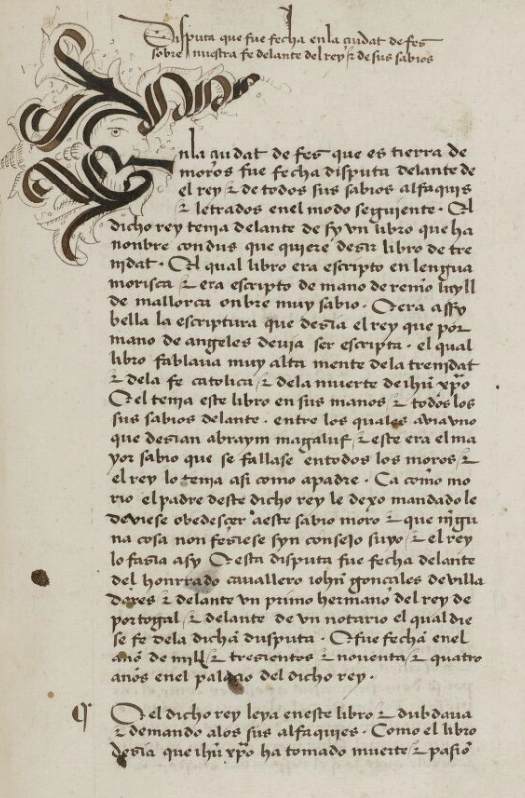
\includegraphics[width=0.5\textwidth]{HistoireIslamMediterranee/Images/DisputaFez1.png}
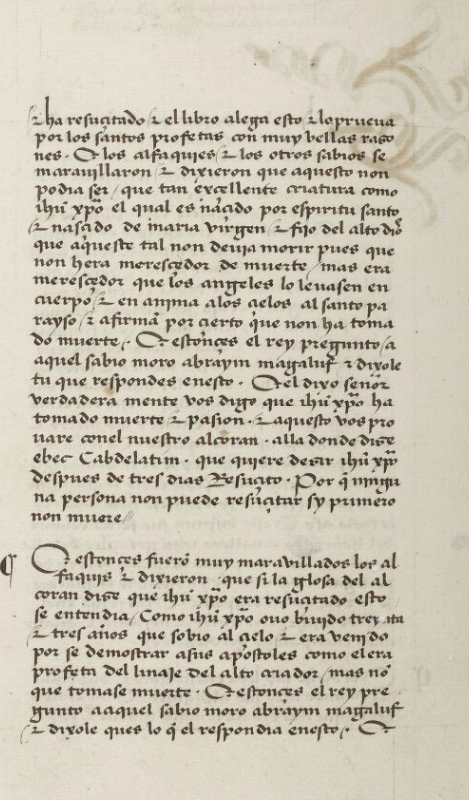
\includegraphics[width=0.5\textwidth]{HistoireIslamMediterranee/Images/DisputaFez2.png}
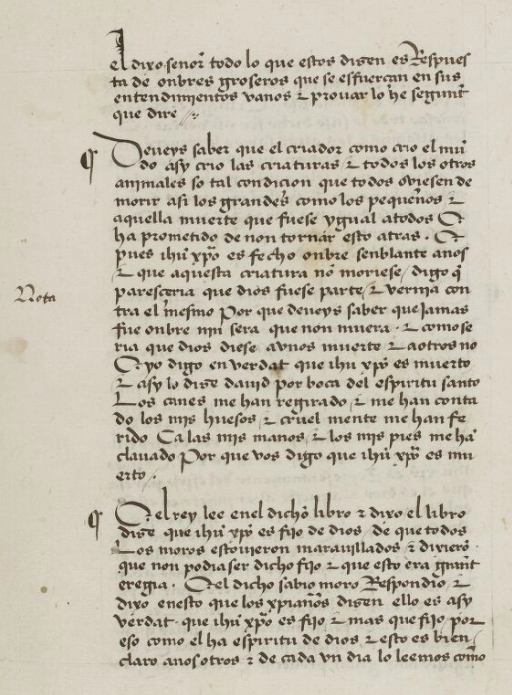
\includegraphics[width=0.5\textwidth]{HistoireIslamMediterranee/Images/DisputaFez3.png}
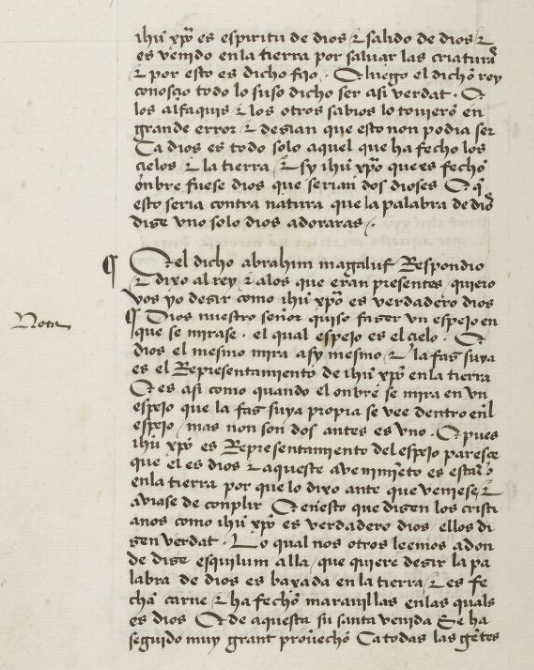
\includegraphics[width=0.5\textwidth]{HistoireIslamMediterranee/Images/DisputaFez4.png}
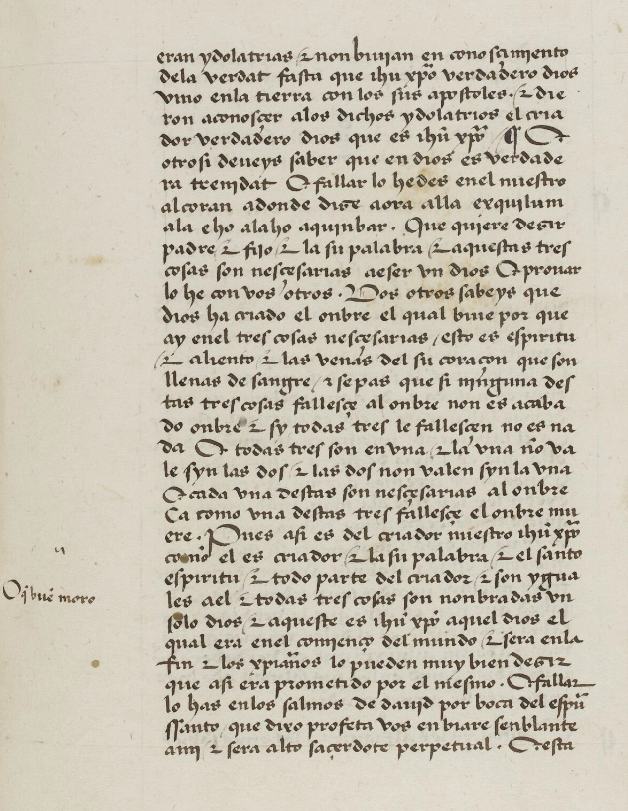
\includegraphics[width=0.5\textwidth]{HistoireIslamMediterranee/Images/DisputaFez5.png}
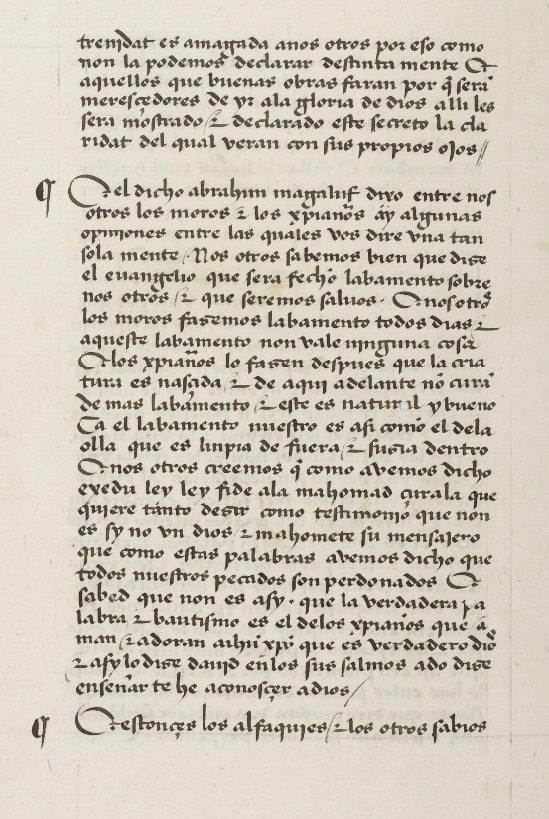
\includegraphics[width=0.5\textwidth]{HistoireIslamMediterranee/Images/DisputaFez6.png}
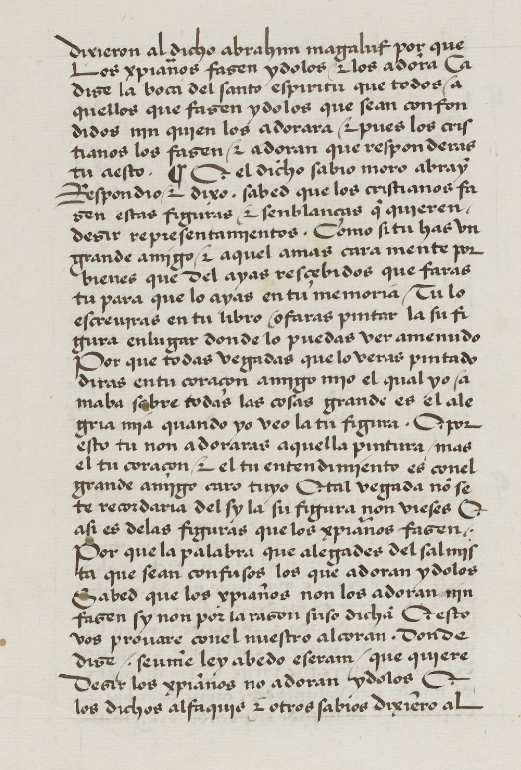
\includegraphics[width=0.5\textwidth]{HistoireIslamMediterranee/Images/DisputaFez7.png}
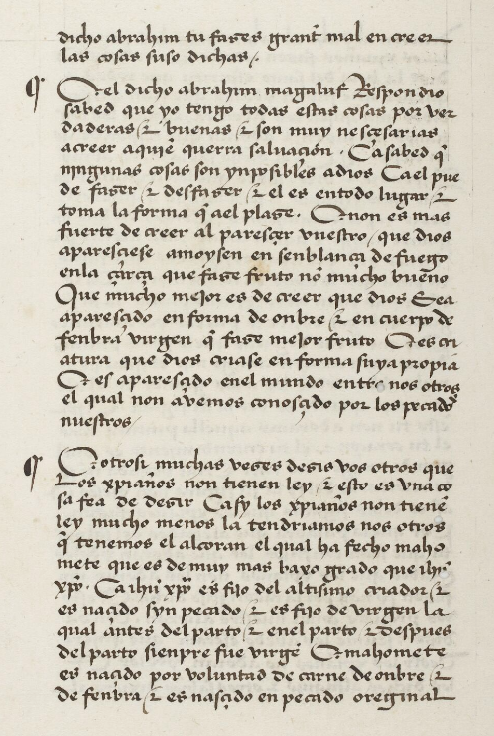
\includegraphics[width=0.5\textwidth]{HistoireIslamMediterranee/Images/DisputaFez8.png}
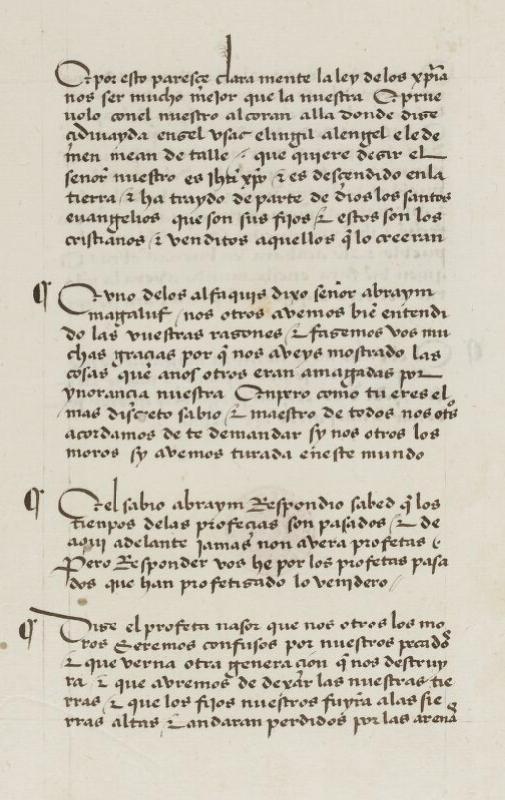
\includegraphics[width=0.5\textwidth]{HistoireIslamMediterranee/Images/DisputaFez9.png}
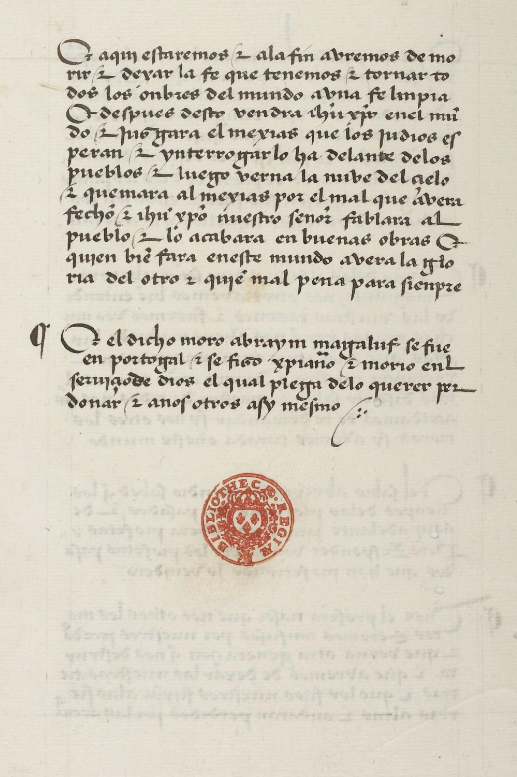
\includegraphics[width=0.5\textwidth]{HistoireIslamMediterranee/Images/DisputaFez10.png}
 
 
    \begin{longtable}{p{.48\textwidth}p{.48\textwidth}}
        Devete sapire che ne la dicta cità de Fes, d1'è in terra de'  r. 52.
Mori, fo facta disputatione denanci el Re e li suoi savi et ho  mini licterati sopra la fé nostra. E lo ditto Re se fe' portare in presencia sua un libro chiamato in lengua morescha <Conclus>,
5) che tanto significa corne <Libro de Trinità», il quale libro era scripto per mano de Raymundo Lull, naturale de l'île de Mayorica, Chrétien homo molto diligente. E parea tanto bella la scnptura che 'l Re dixe spesse volte essere scripta per mano de Dio; el quale libro profundamente tractava de Trinità e de la
10) sancta fé catholica et ancor de la morte de Jésus Christ. Et tenendolo el ditto Re nelle soe mano inseme con tucti suoi lic  terati, tra li guali havea un chiamato Abraym Magaluf, il.,,'quale era sopra tutti fontana di alta sciencia tenuto e reputato per lo Re corne a padre e pcr lo comune vuJgo per propheta. Per cio
15) che quando el Re vechio, padre del dicto Re, venne al morire, lasso et incarico al ditto suo fils , sotto pena de obediencia, che non facisse niuna cosa sença consiglyo de uesto savio moro.
E coss1 fe' e multo lo honoravano. Et ! la supra icta disputatione  1, 53 ,.
fo  fatta in conspetto del magnifico Johanne Gonçales de Villa
20) Dares e denanci a un fratello consobrino del Re de Portogallo e de un notaro il quale facesse fé de la ditta dispntatione, la quale fo facta nela ditta cità de Fes ne li milli ccc. xxxxiiii. nel palaço del ditto Re. E lo ditto Re, tenendo questo Libro de Trimtà ne le mano, legea in quello e, dubitando, domando alli
& Il faut savoir que dans la ville de Fes, en terre des morres, fo facta disputatione dénonce le Roi et ses sages et j'ai des mini litterati sur notre foi. Et ledit Roi fit porter devant lui un livre intitulé en langue mauresque <Conclus>,
5) ce qui signifie autant que <Livre de la Trinité», lequel livre a été écrit par la main de Raymundo Lull \sn{Raymon Lulle, Majorcain, Durant ses voyages, il écrivit de nombreuses œuvres pour démontrer ce qu'il considérait comme des erreurs des philosophes et des théologiens des autres religions. En partant de propositions communes aux trois religions du Livre, il montrait par combinaison que d'autres propositions étaient ou n'étaient pas compatibles avec ces premiers prédicats. Ses interlocuteurs qui acceptaient une proposition en apparence inoffensive étaient obligés de se rendre à ses conclusions. Il tenta également de fonder de nouveaux monastères catholiques dans les contrées qu'il visitait.}
, naturel de l'île de Mayorica, un homo Chrétien très diligent. Et l'écriture paraissait si belle que le Roi disait souvent qu'elle était écrite de la main de Dieu ; dans lequel livre traite en profondeur de la Trinité et de la
10) sancta fé catholica et ancora de la morte de Jésus Christ. Et ledit roi le tenant dans sa main avec tous ses licenciés, parmi eux il y avait un appelé Abraym Magaluf, le vuJgo per propheta. Ainsi
15) que lorsque le vieux Roi, père dudit Roi, vint à mourir, il partit et confia à son fils, sous peine d'obéissance, de ne rien faire sans l'avis de ce sage brun.
Et il fit ainsi, et ils l'honorèrent grandement. Et! le supra icta disputee 1, 53,.
réalisé en présence de la magnifique Johanne Gonçales de Villa
20) Donner et en espèces à un frère consobrine du roi du Portugal et à un notaire qui fait confiance à la société dispntatione, qui se fait en société de Fes dans le milli ccc. xxxxiii. dans le palais dudit Roi. Et ledit Roi, tenant ce Livre de Trimtà dans sa main, legea en lui et, doutant, demanda au
\\

25) soi savij alfaquini che am ditto libro dicea; gly quali nulla raione chiaramente sapeano dare. Et in quest'hora il ditto Re chiamo il ditto Abrahym Magaluf, il quale era maiore in sciencia de tutti quanti, e dixeli in substancia corne il libro dicea che Jésus Christ prese morte e passione per l'humana natura e che resu-
30) scito. E questo allegava il libro e provava per li sancti propheti con belle raxone. E Ji ditti savi che stavano in presencia del ditto Re forte se maraveglyaro e dixero che questo era impossi  bile e che tanto excellente creator corn'era Jésus Christ, nato per Spiritu Sancto dala Sacratissima Maria Vergene, havesse de
35) morire secondo che morte non meritava. Anci li convenia in corpo et in aria essere levato alli cieli ne] sancto paradiso, e affirmavano per certo quello non haver patuto morte. Li qual parole intesi per lo ditto Re, desiderando sapere la intencion del ditto Abrahym Magaluf, dixe: «Tu che dice in questo?» El quale
 & 
         
25) soi savij alfaquini qui m'a dit ce livre; gly que rien de la raison n'a clairement su donner. Et à cette heure le dit Roi appela le dit Abrahym Magaluf, qui était supérieur en science à tous, et dixeli en essence comme le livre dit que Jésus Christ prit la mort et la passion pour la nature humaine et qu'il ressuscita
30) Scythe. Et celui-ci a attaché le livre et a prouvé pour les sancti propheti avec un beau raxone. Et les dieux sages qui se tenaient en présence dudit roi fort s'émerveillèrent et dirent que cela était impossible et qu'un créateur aussi excellent que Jésus Christ, né par Spiritu Sancto de la Très Sainte Vierge Marie, avait de
35) mourir selon lequel la mort ne méritait pas. Même il leur convenait de corps et d'air d'être élevés au ciel dans le saint paradis, et ils affirmaient avec certitude qu'ils n'avaient pas subi la mort. J'ai entendu ces paroles par ledit Roi, désirant connaître l'intention dudit Abrahym Magaluf, il a dit: "Que dites-vous en cela?" El qui
         \\
    El quale
40) Abrahym, indriçando le sue parole al ditto Re chc lo havea in  terrogato, dixe: «Per certo ve dico che Jésus Christ prese morte e passione. E questo ve pruvo per lo mio Alchoram, dove dice
  
Ebe cabdelatim, che, retornandolo in vulgare, vol dire che Jésus Christ dopo de lre di resuscito. E manifcstamente appare che niuna persona po resuscitare se primo non more».  Et in  quel
puncto gly mori alfaquini stetero molto ammirati. Et respoxe un de loro dieendo per tutti: Che ancor che la I glosa de l'Alchoran dicesse che Jésus Christ resuscito, questo se intendea corn'ebbi
passati xxxiii. anni volse ascendere al ciclo c che non vinne per altro se non per demostrarse alli suoi apostoli com'era propheta de lo lignagio de l'alto creatore, ma non che patisse morte. Odendo el Re queste parole dixe al supraditto Abrahym: «Orche dice tu in questo»? Respoxe el ditto: \begin{quote}
    «Signor, quante cose questi dicano son resposte de persone grosse e pocho intelligentJ che se sforçano dire. Et intendol provar secondo oderiti»
\end{quote}. «Signor, dixe el ditto moro, quando el creator creo il mundo e l'homo e l'animali e tutte l'altre creature, fecili con tale conditione che tutti posissero morire, coss1 li grandi corne gly piccoli, e che co  mune a tutti fosse la morte, e. questo promise non tornar in  drieto. Adonque po' che Jésus Christ è fatto hom simile a noy e che non morisse, dicote che parerebi Idio essere parte e vene  rebi contra se stcsso. Et ancor più te dico chc may fo hom ne serà che non mora. E corne poterebbi essere che Idio donassi ad uni morte et ad altri no. E percio trovo in verità Jésus Christ essere morto, e questo confirma el propheta David per boccha del Spiritu Sancto: Li cani me hano ragirato et hanome contato gly mei ossa crudelmente, me hano ferito cbé le mie mano e gly mei pedi me banno chiavati. E per guesto ve dico che cer  tamente e morto».      & El qui
40) Abrahym, adressant ses paroles audit Roi qui l'avait interrogé, dit: «Je vous dis avec certitude que Jésus Christ a pris la mort et la passion. Et cela, je vous le prouve pour mon Alchoram, où il est dit
  
Ebe cabdelatim, qui, le ramenant au vernaculaire, signifie que Jésus Christ après de lre di resuscitato. Et il apparaît clairement que personne ne peut être ressuscité s'il ne meurt pas d'abord". Et en cela
puncto gly mori alfaquini était très admiré. Et respoxe l'un d'eux dieendo for all: Que même si le I glosa de l'Alchoran a dit que Jésus Christ resuscitato, cela si voulait dire corn'ebbi
passé xxxiii. ans, il voulut monter au cycle c qu'il ne gagna que pour se montrer à ses apôtres comme prophète de la lignée du haut créateur, mais non pour subir la mort. En entendant le Roi ces paroles, il dit au susmentionné Abrahym : « Où dis-tu là-dedans » ? Répondez à l'idem : \begin{quote}
    « Signor, combien de choses ces gens disent sont les réponses de gens grands et pas très intelligents qui s'efforcent de dire. Et j'ai l'intention d'essayer selon oderiti».
\end{quote} "Seigneur, dit le ténébreux idem, quand le créateur a créé le monde et l'homme et les animaux et toutes les autres créatures, je les ai faits dans une telle condition que tout le monde pouvait mourir, donc les grandes cornes étaient petites, et ce qui est commun à tous était la mort, e. ce qu'il a promis de ne pas revenir. Donc, tandis que Jésus Christs a été fait comme nous et n'est pas mort, vous dites qu'il semble à Dieu d'être une partie et d'être retenu contre lui-même. Et même plus je vous dis qu'il se peut que pour lui il ne meure pas. Et comment se pourrait-il que Dieu ait accordé la mort à certains et non à d'autres. Et donc je trouve en vérité que Jésus Christ est mort, et cela est confirmé par le prophète David par la bouche du Saint-Esprit : Les chiens m'ont volé et ont cruellement compté mon nom avec mes os, ils m'ont blessé avec mes mains et mes pieds ils m'ont battu. Et pour cela, je vous dis qu'il est certainement mort. \\
E tutti l'altri mon concederono e con  cordarono col ditto sagio moro. Dopo el Re legendo el Re nel ditto libro dicea che Jésus Christ era fils de Dio. De la qual cosa tutti li mori furon amirati et dixeno al Re che non era possibile che sia ditto fils perché parerebi grande heresia. E lo ditto savio moro Ahrahym resposc: «In quello che li xpistiani diceno, lor diceno hona ragione e vera clie Jésus Christ
era fils de Dio e più che figlyo, per cio che I lui tene spiritu
de D10. E questo a noy è ben chiaro, et ogni dà lo legemo, corne Jésus Christ è spiritu de Dio et è enscito da Dio et in terra è dexciso per salvare la natura humana. E per questo è ditto fils ». Et mcontenente el ditto Re conob1 questo essere in verità per le propationi sopradicte.
Eli alfaquini e tutti l'altri savi mori ténerlo in grande errore dicendo clie questo no possiva essere perché ldio era tutto solo colui che fe  i cieli e la terra. Et si Jésus Christ chi è fatto
85) homo fosse Dio, serebino doi Dei. E questo serebi contro natura, ché la parola de Dio dice: Un solo Dio adoreray. E lo ditto Abrahym Magaluf respoxe e dîxe: 

& 

Et tous les autres Mons ont concédé et convenu avec ledit sage Maure. D'après la légende, le Roi dit dans ledit livre que Jésus Christ était un fils de Dieu dont tous les morts étaient admirés et dit au Roi qu'il n'était pas possible qu'il soit appelé un fils car ils semblaient être un grand hérésie. Et ledit sage Moor Ahrahym répondit: «Dans ce que disent les xpi stani, ils disent juste et vrai que Jésus Christ
il était un fils de Dieu et plus qu'un figlyo, pour ce que je lui tene spiritu
de D10. Et cela est très clair pour nous, et tout le monde donne le legem, car Jésus Christ est l'esprit de Dieu et est venu de Dieu et a été décidé sur terre pour sauver la nature humaine. Et pour cette raison, on l'appelle fils ». Et l'homme contenant ledit Roi savait cet être en vérité par les propositions ci-dessus.
Eli Alfaquini et tous les autres sages l'ont gardé dans une grande erreur en disant que cela ne pouvait pas être parce que Dieu était tout seul qui a fait les cieux et la terre. Et si Jésus Christ qui est fait
85) homo était Dieu, serebino doi Dei. Et cela était contre nature, car la parole de Dieu dit : Vous n'adorerez qu'un seul Dieu. Et le idem Abrahym Magaluf respoxe e dîxe : \\

«Gly xpistiani diceno che Jésus Christ è vero Dio e dicono verità. El quale noy legemo dove
&

« Les Gly xpistiani disent que Jésus Christ est le vrai Dieu et ils disent la vérité. El que nous lisons où \\
dice: Esquilitimus alla; chc vol dire: la parnla de .Dio è discesa
90) in nela terra et è fatta carne et ha fatte maraviglyose cose, in ne]i quali è Dio. Et devete sapire cbe ldio è ,·cta Trinità; e qucsto troveray ne] nostro Alchoran dovc <lice: Aora alla cxquilim ala co alaho aquibar; che,·o'  dire: Padre c figlyo e la sua parola. E 'lueste tre cose son necessaric ad esserc un Dio. E questo pro-
95) viro con vui altri. Voi doveti sapire che Tclio ha creato l'homo, i] quale vive in qucsto mundo, che in quello son trc cose nc  cessarie: cio è spirituali e fiato e le,·ene del rore che son pieni de sangue; et è manifesto chc s'alcuna de queste trc cose manca è niente, e se tutti tre cose mancano tanto pegio, e tut.te t:re
100) son necessaric, e l 'una sença li doi no valc c manco Ji doi sença l'una. E ciascuna de queste son neces:;arie a l'homo. E quando l'una de queste manea l'homo more. Adonque eoss, è de] crea  tore nost:ro Jésus Christ corne lui è creatorc c la sua parola è lo Spiritu Sancto e t-utto procedc daJ crcatore c sono equali a Hui.
105) c tutti tre son chiamati  un solo Dio,  chi  cra  in  ne] 1 principio  1. s .
delmundo e serà in ne La fine. E quello che li xpistiani dicono è multo verità grande, ché coss1 era promesso per Dio, la qua! cosa troveray ncgly psalmi de David per bocca del Spiritu Sancto, quai dixe: «Propheta vc mandero simile a me e serà alto sacer-
110) dote pcrpetuale. E. devete sapire cbc le dittc cose significano Trinità, con tutto che sia a noy secreta. Pertanto corne sia di  stinctamente non se puù per noy dcclara.rc. E quelli che ben adoprano anderanno alla gloria de Dio, dove serà dcclarato e mostrato questo secreto; el quaJc secret·o Yederanno apertamentc
115) con li suoi proprij ochi». &

dit : Esquilitimus alla ; ce qui signifie : la parole de Dieu est descendue
90) sur la terre, il s'est fait chair et a fait des choses merveilleuses, dans lesquelles Dieu est.Et vous devez savoir ce qu'est Dieu, la Trinité; et ceci vous trouverez dans] notre Alchoran où <lice: Aora alla cxquilim ala co alaho aquibar; cela,·ou' dire : Père c figlyo et sa parole. Et ces trois choses sont nécessaires pour qu'il y ait un Dieu.
95) Je vis avec vous autres. Vous devez savoir qu'il a créé l'homme, qui vit dans ce monde, que dans ce monde il y a trois choses qui ne sont pas nécessaires : c'est-à-dire les esprits et le souffle et les flammes qui sont pleines de sang ; et il est clair que s'il manque l'une de ces trois choses, ce n'est rien, et s'il manque les trois choses, c'est encore pire, et tout
100) ils sont nécessaires, et le una sença li doi no valc c manque Ji doi sença l'una. Et chacun d'eux est nécessaire : des airs à l'homo. Et quand l'un d'eux affecte davantage l'homo. Par conséquent, il est de] notre créateur Jésus Christ car il est créateur c sa parole est le Spiritu Sancto et tous les procédés du créateur c sont égaux à Hui.
105) c tous les trois sont appelés un seul Dieu, qui cra in ne] 1 principe 1. s .
delmundo et sera dans ne La fin. Et ce que disent les xpistiani est une très grande vérité, car cela a été promis par Dieu, ici ! que trouverez-vous ncgly psaumes de David par la bouche du Spiritu Sancto, quai dixe: «Propheta vc j'enverrai semblable à moi et il sera grand prêtre-
110) dot perpétuelle. E. vous devez savoir comment les choses dictées signifient la Trinité, avec tout ce qu'elle nous est secrète. Donc comme d'instinct c'est pas possible pour nous dcclara.rc. Et ceux qui font bien iront à la gloire de Dieu, où ce secret sera déclaré et révélé ; el quaJc secret · ou ils donneront ouvertement
115) de ses propres yeux». \\

Et ancor pit1 il di tto Abrahym Magaluf dixe al Re et a quelli chi presenti erano: «Io ve voglyo mostrare el vero Dio nel mundo. Dio nostro signore volse fare un spechio, cio è nel cielo in ne] qualc mira sé stesso, e la faça sua è re  presentatione de Yhcst1 Christ in  nc]a terra; è proprio cuss1 como
120) qui ]'omo se mira in uno spechio e rnde m dcntro sua propria
similitudine, ma gi11 pcr qucsto 11011 sono doi, ma 11110. E po' che  Jésus  Christ è representationc del spcchio pare eb·è Dio. E questo aveuimento è stato a la terra pcrchè  nante che vcnissc
]o dixe et era necessario se haYcsse de scquire. e de quesla sua
125) sancta venuta se ne ha scquito grande utilill1; tuui Ji gcnti erano ydolatri e non veniano in co11oscimento de la verità finché Jésus Christ venne in ne la terra, il quale con gly,moi apostoli det  tero a conoscere a li ditti ydolatri cl crcatore vostro Dio essere Jésus Christ)).
&
Et encore plus le dito Abrahym Magaluf dit au Roi et à ceux qui étaient présents : « Je veux te montrer le vrai Dieu dans le monde. Dieu notre seigneur a voulu faire un miroir, c'est-à-dire qu'il est dans le ciel en quelque point de lui-même, et son visage est la représentation de Yhcst1 Christ dans n]a terre ; c'est juste cuss1 como
120) ici l'homme se regarde dans un miroir et se voit dans son propre
similitude, ma gi11 pcr qucsto 11011 sono doi, ma 11110. C'est juste que Jésus Christ est la représentationc du miroir semble-t-il et il est Dieu. Et cet événement était sur terre parce que nante que vcnissc
]o dixe et était nécessaire si haYcsse de scquire. et de celui-ci son
125) sainte venue, il en a fait grand usage1; tous les Juifs étaient des idolâtres et ne sont pas parvenus à la connaissance de la vérité jusqu'à ce que Hest1 Christ soit venu sur la terre, qui avec gly, nos apôtres ont fait connaître aux idolâtres que le chercheur de votre Dieu était Yhesu Christ)). \\
    \end{longtable}
 

%\chapter{Ecologie et Religions - Colloque IDEO 2022 }
\mn{pour célébrer les 20 ans de la bibliothèque - Le Caire}

\section{M. Aziz Hilal}

\paragraph{Aziz Hilal} il est philosophe, il est membre de membre de l'IDEO, philosophe, il enseigne l'arabe et la philosophie au lycée français du Caire et il est un passionné d'Al Farabi. Il a fait sa thèse de doctorat sur Al-Farabi. Il en est un lecteur précis et qui essaie de faire justice à ces textes qui parfois sont lus de manière un peu biaisée.

\paragraph{Qu'est ce que l'écologie ? Qu'est ce que la création en soi ?}

\paragraph{Thèse d'Hercule}Je commence tout de suite par une thèse qui me passionne. C'est celle de Thomas Bower que je découvre et qui s'appelle cette thèse \textit{Der Kultur der Ambiguitate}. Tour de l'ambiguïté. La culture de l'ambiguïté pour dire que l'islam, en quelque sorte, avant un peu les textes qui ont été fixés une fois pour toutes était un continuum.
Ça veut dire qu'il y a sur la nature. Vous allez voir qu'on voit tout trouver. D'abord, on parle de protection de la nature ou de l'environnement. Le mot qui veut dire environnement, c'est a n'existait pas, il n'était pas utilisé dans une autre signification. On parlait de beit. Cela veut dire la maison et par extension, c'est fonder une maison.
Alors c'est très important. Partir par là. Le mot nature n'existe pas comme tel dans le Coran par exemple. Alors qu'est ce qui existait ? Existait un mot qui compte, qu'on a trouve, qu'on a soustra (?), qu'on a traduit par la nature. Mais ce n'est pas une traduction exacte. Je ne sais pas la peine, ça veut dire c'est pas la peine de rentrer dans le détail lexicographique album de la nature que Dieu a donné à chacun de nous au début de la création, est ce qui décide un peu de la nature de chaque homme. Al feltra
Est ce que ce qui est présent, ça peut être en fait en pour parler de la nature, il n'y avait pas le signifiant. Bien sûr, il y avait le signifié. Je commencerai par un verset coranique que tout le monde utilise pour dire que finalement, on trouve dans le Coran quelque chose de le côté de l'environnement. Dans la sourate deux, vers 30,
\begin{quote}
    2 : 30 - Lorsque Ton Seigneur confia aux Anges: "Je vais établir sur la terre un vicaire "Khalifa". Ils dirent: "Vas-Tu y désigner un qui y mettra le désordre et répandra le sang, quand nous sommes là à Te sanctifier et à Te glorifier?" - Il dit: "En vérité, Je sais ce que vous ne savez pas!".
\end{quote}
  Là je traduis. Donc quand Dieu a dit je vais établir sur terre, il y avait le mot terre, pour la nature sur terre indiquée ou bien un sous réseau. Et les anges ont riposté. Seniors, vous allez mettre quelqu'un qui va semer le désordre, vous allez mettre quelqu'un - je traduis presque mot à mot -.
vous allez mettre quelqu'un qui va se porter et qui va répandre le son alors que nous, les anges, on vous glorifie et on vous sanctifie. Et Dieu a fini par dire :
\begin{quote}
     je sais ce que vous ignorez.
\end{quote}
 Alors cette histoire de Dieu a établi sur terre un vicaire, un sous régent, ça veut dire lui a confié un dépôt sacré pour s'en occuper en quelque sorte.
L'homme, dans un autre verset, était un petit peu naïf. Il a accepté ce dépôt sacré parce qu'il a été au départ confié à toute la nature. Nous avons exposé le dépôt sacré Amana à à tous, sur tous les cieux et les terres. Ils ont refusé, mais l'homme a accepté.
Alors l'homme a accepté d'être le vainqueur, d'être le sous régent pour s'occuper de la terre. Même si les Anges ont un peu mis en garde le Seigneur. Attention, peut être que vous allez mettre quelqu'un qui va répandre le sang et  qui va mettre le désordre, ça veut dire qu'il va mettre du désordre dans la nature.
Dans le Coran, il  y a toute tous les éléments de la nature, mais il n'y a pas la nature en tant que tel, Il n'y a pas le mot, il le prouvera. Après, en philosophie, on ne le trouve pas dans le Coran. Il y a tous les éléments de la nature. La nature est quelque chose, la nature, il y a quelque chose de le Coran, de ce qu'on appelle.
Tous les Grecs ont appelé le pharmacant. Remarquons que ça veut dire un format quand ça veut dire Dans le caducée d'Hermès, vous avez les deux serpents qui se font face, un qui représente bien sûr la bienfaisance et l'autre qui représente la toxicité. C'est la nature qu'on trouve dans le Coran. La nature est quelque chose d'agréable.
La nature est quelque chose de recèle beaucoup de beauté.   Mais en même temps, vous voyez la beauté en même temps, cette beauté là. En même temps, ces lampes là, ils sont vraiment des projectiles pour chasser les démons. Vous voyez le sens de Fatma quand c'est comme ça, la nature, la nature qui va être glorifiée.
D'un côté, ça veut dire tous les grands peuples qui sont dans l'histoire, Dans le Coran, ils ont arrivés à un point presque de maîtrise de la nature de la mettre à leur merci. Si on parle par exemple de peuples, de tabou, de peuples, d'autres, les peuples de Al, c'est des gens qui ont fondé une ville extraordinaire qui s'appelle Ams, aux colonnes.
Paraît il que c'est une ville à plusieurs étages, même à des sous sols, et on ne sait pas où il est. Mais qu'est ce que ça veut dire ? Les éléments de la nature ont été. On a fait que les éléments de la nature pour la nature obéissent au même temps, parce que ces peuples là n'ont pas compris le message divin, n'ont pas écouté les envoyés de Dieu.
C'est la nature elle même qui va se retourner contre eux. Et on trouve que la nature, le peuple Al, par exemple ont été décimés par un vent de sept jours, un vent violent. Vous voyez les deux côtés de la nature, mais la nature belle finalement, et la de ce modèle 

\paragraph{Paradis}et ce modèle, bien sûr, c'est le paradis avec les rivières limpides, avec le miel des rivières de miel, avec les rivières de lait, avec les quatre voies sont connues pour les Arabes.
Vous savez que c'est un milieu austère. Et quand on parle de miel et d'eau extraordinaire, ça, c'est l'image de la nature parfaite. Cette nature parfaite. Finalement, vu qu'on vivait dans un désert, qu'on vivait dans un milieu austère, c'était presque le modèle et le rêve. Et tout ce qui pourrait exister sur le sur terre et éphémère. Et c'est ce paradis, cette nature idéale, cette nature extraordinaire.
C'est cette nature qui va être célébrée par de grands poètes et les Arabes auront quitté le désert. Bien sûr, les musulmans ont quitté le désert, ils sont allés au l'Andalousie et en temps, le tout d'apprécier la nature. Les meilleurs poètes d'aventures se trouvent l'Andalousie, ça veut dire cette terre qui va de Saragosse à au sud de Porto, la ligne qui va un peu, surtout au neuvième Xᵉ siècle.
Après, on va, descendra pas vers le bas. Il y a un grand poète xxxxx, qui a vécu à Saragosse et après qu'il va partir vers Valence quand il y avait avoir le mouvement de la Reconquista. Mais c'est bien sûr qu'était loin de toute l'histoire de guerre, est un vrai, pourrait être un vrai troubadour. D'ailleurs, il a vu quelque chose des troubadours et raconte une histoire extraordinaire et disait au Andalou : "profitez vous, profitez de cette nature.
Personne d'autre ne l'a pas vu là. Un paradis sur terre". 

Alors je vais vous donner le poème en arabe, je le traduis.  vous avez les gens de l'Andalousie, vous avez l'eau, vous avez des ombrages, vous avez des rivières et vous avez des arbres.
Je crois que le paradis, c'est vous qui est la posséder encore. Et si on m'avait demandé à choisir, c'est ce paradis que je choisirais. Ça veut dire si on m'avait donné le choix entre les deux paradis, paradis céleste, le paradis terrestre choisirait le paradis terrestre et après lui, je continue en traduisant. Il dit finalement N'ayez pas peur, le feu de la géhenne est loin de vous, parce qu'aux hommes, quelqu'un qu'on a introduit au paradis ne peut goûter le tout ne peut subir les flammes de la géhenne.
Alors c'est sûr. Mais bon, quand on l'Andalousie, on l'appelle d'ailleurs à , on l'appelle maintenant le paradis perdu.  


C'est cette nature qu'on a perdu, qu'on pleure quand tous les poètes ont vraiment pleuré. 

\paragraph{Philosophie} Troisième volet Je pense maintenant à la philosophie seule en matière. Je veux parler de la philo, de la nature en philosophie bien sûr. Chez les juifs, c'est dans la culture arabo musulmane, pas les autres.  la nature n'a rien à voir avec la nature telle qu'elle a été développée chez les Grecs.
Ça veut dire la nature a ses propres lois et est indépendante. 

\section{Emmanuel Pisani - Al-Ghazali et Ecologie}
\label{theol:AlGazali25}

    \paragraph{Les Ecrits de Ghazali sur l'Ecologie sont rares}Pour une protection possible de la nature, de la manière dont il convient de penser la relation de l'homme à son environnement, à la création des données. Dans quelle mesure le Ghazali pourrait il permettre l'éclosion d'une pensée écologique islamique qui partirait de sa théologie en trois en trois points ? Le premier, c'est d'abord en vue d'un constat : nonobstant l'importance de notre auteur, Les écrits sur la Création de Ghazali dans l'islam sont très rares : elles ne sont pas inexistantes justement - x ont attiré mon attention sur un de ses articles publié récemment où il est cité.
Elles ne sont pas inexistantes, mais elles sont rares, marginales. Alors pourquoi est ce que ce serait dû à la nécessité ? Le signe que la nécessité de restreindre les appétits de l'homme dans son usage des biens de la création n'est jamais abordée dans ses écrits ? Il est vrai qu'il n'y a pas de \textbf{théologie de la nature} qui appellerait à une attention ou une protection chez lui.

\paragraph{Question non posée : la création au service de l'homme}

    

Alors Al-Ghazali ne connaît pas la question l'anthropocène, capacité qu'a l'homme à modifier son environnement, L'extermination des dodo ? Il ne connaît pas. 
Je dirais même que pour lui, la création, au contraire, est un réservoir infini de biens disponibles pour l'homme. Et c'est le signe même de la manifestation, de la bienveillance, de la bonté, de la bienfaisance de Dieu à l'égard de l'homme que de lui donner.
Tout est là pour l'homme à son service. Et si Al-Ghazali envisage l'activité désordonnée de l'homme, elle ne saurait de toute manière avoir des répercussions décisives sur la création. 

\paragraph{Théologie de l'action}

  Pourtant, et c'est mon deuxième point, il y a chez lui une théologie d'action qui n'est pas sans incidence pour notre sujet. En effet, et dans sa réflexion, c'est un théologien.
Il part donc de Dieu. Il constate que méditer sur l'essence de Dieu qui est Dieu, ce n'est pas possible pour l'homme . Une méditation sur l'essence divine et pour mieux se faire comprendre. Peut être que je vous ai déjà perdus en disant cela. 
\begin{Ex}[Raisonnement de la mouche]
Il va donner l'exemple prosaïque de la mouche. Là, je vous l'ai retrouvé.
Si on lui disait à la mouche que son créateur  ne possédait ni des ailes, ni même ni pied, ni capacité à voler, elle le trouverait plus imparfait qu'elle même qu'elle n'est. 
\end{Ex}
Or, malheureusement, déplore Al-Ghazali, ce raisonnement, le raisonnement de la mouche et celui de la majorité des hommes. Et comme il n'écrit pas seulement pour des savants. Il est donc préférable, pour parler de Dieu, non pas de partir d'une méditation de son essence, mais de ce qu'il crée et donc de la création.
\paragraph{Nous sommes insensible à la beauté de la Création}
Aussi, il l'invite à une méditation sur la création. Et dans cette optique, la création, vous le voyez, n'est pas seulement uniquement la disposition de l'homme pour satisfaire ses besoins, mais elle est là pour \textsc{permettre à l'homme de retrouver le chemin du Créateur et admirer la grandeur de Dieu}, grandeur qui suscite la gratitude et l'adoration. Alors, bizarrement, déplore Al-Ghazali, les hommes trouvent beau devant un tableau peint par des hommes par des mains d'hommes, Mais ils restent insensibles à l'artisan des merveilles de la création.
\paragraph{C'est Dieu qui écrit dans la Création}
Chez lui, c'est grâce à lui, la création acquiert un véritable statut théologique. La méditation sur les choses créées vient ainsi tempérer l'image d'une pensée où la création ne serait là que comme un réservoir disponible à l'homme pour sa consommation et son confort. La création, au contraire, acquiert une qualité qui implique une attention, parce qu'au delà de la chaîne des causalités, il s'agit de découvrir qui est Dieu écrit.
Tous les êtres vivants sont des effets de la puissance de Dieu et une des lumières de son essence. Il n'y a rien de plus obscur que le néant et de plus lumineux que l'existence. L'existence de toute chose est une des lumières de l'essence de Dieu. 
\paragraph{la méditation transforme}La \textit{méditation} est donc pour le Ghazali, le chemin de l'illumination. Elle permet d'accéder à la connaissance divine, ce qui n'est pas sans incidence profonde pour l'homme.
Les passions de son cœur sont alors transformées. Les facultés de la vision intime intérieure développée par ces lumières divines auxquelles il accède. La perspective est clairement celle du soufisme. La méditation sur le créé permet voir ce pas visible du premier coup d'œil et l'ouvre à la possibilité un spirituel plus élevé. Mais quid ? Quid de son comportement à l'égard du Christ ?

\paragraph{Ascèse si méditation du Christ}
Si ce chemin d'illumination passe par la méditation du Christ ?\textsc{ Il est inséparable. Mesdames et messieurs, je vous le dis  d'une certaine ascès}e. Pour souligner le lien, Al-Ghazali s'appuie sur une tradition prophétique qui dit que la méditation sur les choses créées est la moitié de l'adoration. Mais le peu de nourriture, l'adoration entière. Ainsi, pour lui, la méditation de la création met sur la voie de l'adoration, adoration qui n'a que plénitude par la saisie.

\paragraph{l'ascèse régule nos appétits}
C'est mon troisième point. L'ascèse, en effet, est au cœur du dispositif du chemin spirituel qui conduit vers Dieu. Chez Al Ghazali, l'ascèse régule nos appétits et plus encore dans une perspective fonctionnaliste. Alors Ghazali va justifier la nécessité d'éprouver la fin. Et mesdames et messieurs, il va distinguer dix bonnes raisons d'éprouver la fin. Alors, je vous les livre ce soir, avant notre cocktail dînatoire.
\begin{itemize}
    \item Premièrement, elle purifie le cœur et oui, elle anime le tempérament et à la fuite, le regard intérieur. Alors que la satiété provoque l'apathie, elle aveugle le cœur et donc brûle le cerveau. Ainsi, l'ascèse ouvre à la connaissance des réalités divines.  
    \item Deuxièmement, la purification du cœur prépare à l'émotion de l'énoncé de l'énoncé de Dieu. Souvent, on prononce le Dieu, mais sans s'en délecter.
Mais celui qui a faim, quand il convoque le nom de Dieu, il le fait avec délectation.    \item Troisièmement, la fin suscite la crainte de Dieu. Elle brise lames dans le sens de son impudence, de son orgueil, de sa rébellion à l'égard de Dieu ou de son oublie de Dieu. Mais la foi permet à l'homme de voir son impuissance, sa faiblesse et elle redonne toute sa place à Dieu.
    \item Quatrièmement, la faim permet de se souvenir des épreuves qui attendent ceux qui sont éprouvés par Dieu. Elle rappelle les tourments de l'au delà et elle crée une solidarité avec ceux qui ont faim ou. Pourquoi tiens tu autant à la faim alors que tu possèdes les trésors de la terre ? Le Prophète répondait J'ai peur de manger à ma faim et d'oublier ceux qui souffrent.
Ce qui en souffre.     \item Cinquièmement, elle permet d'affaiblir les passions liées aux actes de désobéissance. Au fond, la faim de l'homme, la faim permet de contrôler tous ces désirs.     \item Sixième sens permet de repousser le sommeil, de s'habituer à la vie.     \item Septième. Nous, elle facilite l'assiduité à l'adoration. On gagne du temps à ne pas se nourrir et se tend. Pour quoi faire ?
Enfin, pour jouer sur son téléphone portable. Nous sommes au XIIᵉ siècle, mais ce temps pour adorer, pour se recueillir, pour se souvenir du nom de Dieu. On gagne du temps à ne pas faire les courses et à préparer les repas, à se laver les mains et la bouche, à aller plusieurs fois aux toilettes parce que l'on a trop bu et pour manger ?
Oui, avec Al-Ghazali, on est toujours au cœur du quotidien et de tous ces moments.    \item Huitième Non, cela donne la santé car trop de nourriture alourdit le corps et le rend malade. L'ascèse épargne des maladies au corps, épargne les cures de maladies comme l'impulsivité ou d'autres vices.     \item Neuvième un Manger peu. On fait des économies, les prix augmentent. Mangeons moins     
\item et 10ᵉ enfin.
Manger peu ou pas.
\end{itemize}

\paragraph{donner, c'est conserver dans les coffres de la grâce divine}
 L'altruisme nous rend bons envers les orphelins et les pauvres. Toujours avec un esprit très prosaïque, À la Al-Ghazali écrit que la nourriture dont il se nourrit finit dans les latrines, alors que la nourriture dont il fait l'aumône est conservée dans les coffres de la grâce divine. Alors, pour conclure, nous étions partis de la vision consumériste de la création chez Al-Ghazali et visiblement de la difficulté à élaborer une théologie islamique de l'écologie.


 \paragraph{La Création, chemin vers Dieu}
Nous avons vu cependant, à partir de ces livres spirituels qui invitent à voir toute chose comme comportant une sagesse, qu'il s'agisse des étoiles, des mers, des plantes ou des animaux. Pour lui, la création n'est pas d'abord à la disposition des estomacs et des passions des hommes, mais elle est un chemin pour parvenir adieu à la connaissance de Dieu.
Certes, certains abusent, gaspillent, ont un comportement ingrat. Ainsi écrivent critiques. Cassé la branche d'un arbre sans but précis est une ingratitude. Pour autant, il poursuit en disant que l'usage des arbres pour les hommes est conforme à la volonté divine, selon le principe que si l'homme et l'arbre sont tous deux périssables, l'homme est plus noble que l'âme, et il est sage que ce qui est moins noble contribue à la pérennité de ce qui est plus noble.
Si on devait s'arrêter à ce niveau de réflexion, on retrouverait la vision d'une création mise simplement au service de l'homme le plus noble des créatures. 
\paragraph{Aller plus loin en ajoutant l'idée de justice}
Mais il faut aller plus loin et elle va plus loin en y adjoignant l'idée de justice. Ainsi, utiliser l'arbre du voisin, qui donc ne m'appartient pas, est une injustice. Or, rappelle t il, le propriétaire ultime de toute chose créé, c'est qui ?
C'est Dieu ? Ainsi, indépendamment de la main divine, de la bonté de Dieu, celui qui prend au delà de ce dont il a besoin se comporte comme un homme injuste. Le questionnement de Al-Ghazali sur l'écologie n'aura donc pas été vain, et il me semble que l'on peut voir dans ces concepts, dans ces exemples, dans cette réflexion spirituelle, les braises encore chaudes pour penser à partir de cette éthique islamique de la responsabilité, une écologie islamique.
Et commencer à voir un peu mieux notre quotidien des lectures que nous faisons du Coran, de la poésie andalouse, des philosophes, des textes mystiques. 




\section{Adrien Candiard}

\paragraph{Adrien Candiard}
    Nous continuons notre exploration du patrimoine islamique classique avec le frère Adrien. Adrien , qui soutient très bientôt le mois prochain sa thèse de doctorat sur un auteur Très controversé, Ibn-Taymiyya.   Sa passion, Adrien, c'est d'essayer de comprendre comment pensent les gens qui pensent autrement et c'est forcément rationnel. Et donc on peut faire confiance que même les auteurs les plus en apparence délirants, extrémistes, incompréhensibles, ont une rationalité. Il est passionné par cette quête de la rationalité. Comment pensent les autres ? 

    \paragraph{risque de l'anachronisme}
Emmanuel m'a demandé d'intervenir aujourd'hui pour vous présenter ce que peut avoir à nous dire sur les problèmes écologiques contemporains. Le corpus islamique que je fréquente est celui de la théologie islamique médiévale. Je n'ai accepté qu'avec obéissance ou avec un peu de réticence ou peut être par goût du paradoxe, seulement pour les questions de méthode, qui est manuel rappelait le risque de faire des anachronismes tout le temps en lisant des auteurs avec des questions qui ne se posent absolument pas.

\paragraph{le Kalam et son aridité}
Pour éviter quand même des anachronismes complets. Je ne parlerai pas d'interdit aujourd'hui parce que là, vraiment, il y a matière. Mais surtout, rien n'évoque moins l'écologie que les arides traités de théologie islamique, cette science qu'on appelle la science du Kalam, de la parole et qui, à partir du IXᵉ siècle, va s'efforcer de faire rentrer la foi islamique fondée sur le Coran et les hadiths, les traditions prophétiques dans un cadre conceptuel rigoureux, tellement rigoureux à vrai dire, pour ceux qui ont déjà ouvert des traités de Kalam, que dans ces discussions extrêmement techniques, il n'y a pas un guide technique et polémique non plus d'ailleurs parce que plusieurs écoles vont s'affronter, parfois très rudement. 

\paragraph{la Kalam à la différence du Coran est abstrait :  pas de place pour les ours blancs}Et bien dans
ces traités là, il n'y a pas tellement de place pour les écureuils, pour les ours blancs ou pour les autres mastodontes. Plus précisément, on y navigue en général dans un univers d'entités abstraites d'où notre monde concret, avec sa météo, avec ces insectes et sa qualité de l'air, est extrêmement absent. Il y est question de création, bien sûr, dans ces traités, le terme, qui est très employé, mais le terme renvoie à l'acte créateur de Dieu et non pas tellement au ou concret créé par lui dans sa matérialité.
Ce monde concret et matériel est bien présent. Pourtant, dans le Coran, il nous l'a rappelé et fait voir le Coran, d'ailleurs, développe aussi des images apocalyptiques qui peuvent nous donner à réfléchir aujourd'hui. Mais on en trouve à peu près rien dans les textes du Kalam. Ça ne veut pas dire qu'il ne se préoccupe pas du Coran, au contraire, mais il va concentrer son attention sur d'autres aspects du texte sacré des musulmans, et notamment une question de première importance qui saute aux yeux si vous ouvrez le Coran.

\paragraph{Omnipotence de Dieu dans le Coran} Si vous commencez à lire le Coran, c'est un élément qui va vous apparaître immédiatement, même si vous n'êtes pas un spécialiste dans le Coran.
L'omnipotence de Dieu est affirmée de façon absolument massive, totale, inlassablement répétitive. Dieu est puissant sur toute chose. La formule revient comme un refrain. Je crois que je vais trouver une petite quarantaine d'occurrences de cette formule, précise, et bien des versets vont en préciser le sens. Dieu fait ce qu'il veut, il crée ce qu'il veut, il fait le bien.
Il crée le bien, mais aussi le mal. Il châtie et récompense à son gré. Rien n'arrive qu'il ne l'ait voulu.  Il envoie aux hommes bénédiction, mais aussi fléaux et calamités.
\paragraph{Comment réconcilier liberté de l'homme ?}Et cette omnipotence divine, affirmée dans sa version la plus extensive, va poser au premier théologien de l'islam un certain nombre de difficultés, et en particulier parce qu'elle entre en concurrence avec la liberté et la responsabilité de l'homme.
Si Dieu, en effet, crée toute chose et en particulier chacune de nos actions, nous les bonnes comme les mauvaises. Alors, au nom de quoi va t il nous juger ? Au dernier jour, il enverra en enfer les méchants, mais pour des actions qu'il a lui même créées. Bizarre, c'est quand même pas très juste cette tension entre la responsabilité humaine et la toute puissance de Dieu.
\paragraph{Anecdote du Prêt}
On la voit magistralement résumée dans une petite anecdote que je vous raconte, qui est rapportée par un théologien très important du Xᵉ siècle, la charia, qui raconte une petite histoire qui aurait eu lieu en Irak entre un certain Soheib qui avait emprunté de l'argent à un certain Mimoun mais on ne connaît pas les deux par ailleurs. Et Mimoun, évidemment, demande à Soheib de lui rembourser son argent.
t Soheib lui répond \textit{Je te le rendrais si Dieu le veut}. Mimoun n'est pas complètement rassuré et s'appuyant sur une certitude qui est que Dieu veut qu'on rende à chacun ce qui lui revient, lui dit : \textit{Dieu veut que tu me rendes mon argent}. Soheib, s'appuyant sur la toute puissance divine dit : \textit{si Dieu voulait que je demande ton argent, je l'aurais déjà}.

Eh oui ! Ce qui n'est pas sans fin, tout ça, vous voyez. Dans cette petite discussion, on voit l'enjeu essentiel de cette toute puissance divine et on voit qu'en fait les deux ont des bonnes raisons à faire valoir un peu problématique. Alors ils vont aller chercher à s'en remettre à l'arbitrage d'un sage qui est alors en prison et qui va par une réponse écrite, ménager la chèvre et le chou. Ce qui ne permet pas de trancher. 

\paragraph{Conséquence pour la réflexion écologique, chaine naturelle de causes et d'effets}
Cette question théologique et morale est passionnante et je pourrais en parler littéralement des heures, mais je comprend que c'est assez mobiliser l'énergie de théologiens médiévaux. Mais si je vous en parle ce soir, c'est parce que cette envahissante toute puissance de Dieu n'a pas seulement des effets sur la morale humaine. Elle risque en effet de rendre également impossible toute réflexion écologique.
La réflexion écologique, en effet, suppose comme premier préalable l'existence d'une chaîne naturelle de causes et d'effets. Si on réunit la COP 27 , c'est bien parce qu'on constate les effets de l'action de l'homme sur le climat, sur la biodiversité et qu'on espère que d'autres actions ont d'autres effets, ont des effets correcteurs, et cetera Cela nous paraît peut être assez évident cette idée qu'il y a des causes et des effets, mais cette évidence n'est pas partagée.
En effet, la fascination pour la toute puissance divine a pu pousser des penseurs de l'islam, parfois des intellectuels immenses, à minimiser, voire à nier cette chaîne des causes qui régit notre monde. Au profit de quoi ? De l'action immédiate de Dieu, créateur de toute chose à tout instant. Et donc, si ce verre tombe, si je le lâche, ça ne veut pas dire qu'il tombe parce que je le lâche dans cette optique là, parce que ça ferait de moi le créateur d'une réalité.
Cela ferait de moi le créateur de la chute du gobelet. Et certains auteurs vont donc dire non, Pas du tout. Si c'est Dieu qui crée à la fois mon acte de lâcher et la chute du gobelet, si Dieu ne voulait pas activement faire tomber le gobelet, eh bien il ne tombera pas. J'aurais beau le lâcher, le gobelet ne tombera pas.
\paragraph{pour certains, refus de faire une loi de l'univers qui s'impose à Dieu}
Bien sûr, vous avez déjà observé qu'à chaque fois, je pourrais le faire 25 fois devant vous. À chaque fois que je lâche, il tombe et les penseurs dont je parle en sont absolument conscients. Évidemment, ils ont remarqué que ça marchait comme ça, mais il refuse cependant d'en faire une loi de l'univers, la gravité en l'occurrence, qui s'imposerait à Dieu.
Il préfère voir dans la chute du gobelet, à chaque fois qu'on lâche une habitude de Dieu. Dieu qui d'ordinaire fait tomber les gobelets quand on les lâche. Mais c'est toujours un effet de sa libre volonté. C'est lui qui le choisit à chaque fois. Mais voilà, on pourrait tout aussi bien vouloir le contraire, vouloir que ça ne tombe pas sans que cela contrevient à une loi naturelle, physique.
Alors, personne ne le formule comme je vais le faire au Moyen Âge. Mais à l'évidence, une telle conception totalisante de la puissance divine stérilise la possibilité d'une pensée écologique. Si le réchauffement climatique, par exemple, est le résultat de l'action de l'homme et même du péché de l'homme, là dessus, on peut développer une théologie de Pascal au réchauffement climatique. On peut le combattre.
\paragraph{Combattre ou accepter le changement climatique ?}
Peut être même doit on le combattre. S'il est en revanche le résultat de la volonté active de Dieu, alors ce réchauffement, il faut l'accueillir dans la foi, peut être comme une épreuve imposée à l'humanité. Mais on ne peut pas vraiment lutter contre lui, car ce serait alors lutter contre la volonté de Dieu. La seule attitude raisonnable est alors ou pas précisément, comme on le dit parfois, le fatalisme, parce qu'il ne s'agit pas d'une fatalité, mais l'abandon, la contemplation de Dieu dans la réalité qui est devant moi, sans cesse, dans ses beautés comme dans ces calamités qui expriment l'insondable et l'adorable volonté de Dieu.
Mais la théologie islamique classique, la théologie du kalam, a, dans certaines de ses écoles,  essayé de produire des des éléments conceptuels qui rendent pensable cette envahissante toute puissance de Dieu contre la chaîne naturelle des causes et des effets. Mais le même Kalam a aussi vu naître en son sein les plus farouches opposants à cette conception la toute puissance divine, à savoir les représentants de l'école mu'tazilite.

\paragraph{Mu'tazilisme contre toute puissance divine}
Ce courant théologique, né au milieu du VIIIᵉ siècle de l'ère chrétienne, avec en gros l'arrivée au pouvoir des califes abbassides et d'ailleurs, sans doute la première véritable école de théologie au sens propre en islam, qui a cherché à rendre raison conceptuellement de la foi islamique. Ces théologiens ont la réputation parfois trompeuse en Occident, d'être des rationalistes. Je dis trompeuse, car nous entendons facilement par là qu'ils pourraient être un peu athées s'ils sont rationalistes.
Et ce n'est absolument pas le cas. Il s'agit bien de théologiens qui croient que le Coran est la Parole de Dieu, mais qui croit aussi que la raison humaine est un instrument fiable pour comprendre cette parole, pour l'interpréter. l'École mutazilite n'a pas toujours bonne réputation chez les musulmans d'aujourd'hui, du fait d'une importante controverse sur la nature du Coran.
 Mais cette école, qui a du reste disparu du monde sunnite au début du XIIIᵉ siècle, a marqué la pensée théologique islamique à qui elle a donné d'importants instruments de pensée rationnelle. D'ailleurs, depuis le XIXᵉ siècle, un certain nombre d'intellectuels musulmans y font référence et en ont certainement salué l'audace, la liberté de pensée.

\paragraph{pas des partisans du libre arbitre car ne pas penser du point de vue morale} Alors, sur la question de la toute puissance divine. On a voulu souvent faire en Occident des auteurs pour les partisans du libre arbitre de l'homme. Ce n'est pas Dieu qui crée les actes humains, mais bien l'homme qui les produit et qui porte donc la responsabilité de ces mauvaises actions. Alors ce n'est pas complètement faux, mais c'est lire la pensée unique uniquement du point de vue moral, vu la moralité des actions humaines.
Et si ce n'est pas, ce n'est pas complet parce que évidemment ça compte sa dimension morale, mais l'ambition des mu'tazilites est beaucoup plus vaste. Ils ne disent pas seulement que l'homme est capable de faire le bien ou le mal. Ils disent bien une créature est capable de produire un véritable effet dans la création. Ce qui est en jeu, donc plus large, c'est l'autonomie de la création que dureront capables de causes et des faits.
Sans cela, pour eux, la création de Dieu serait incomplète. Elle serait presque fictive. Dieu n'aurait créé qu'un vaste terrain de jeu où sa volonté occuperait toute la place. Au lieu de cela, disent les mots Tassili. Dieu, qui a créé un véritable monde, un monde où entrent en jeu les lois de la physique et la volonté des vivants qui ne sont pas de simples illusions masquant la seule force agissante et la toute puissance divine.
Pour les élites, cette autonomie du monde créé n'est pas une manière d'arracher quelque chose à la puissance de Dieu. Ce n'est pas en concurrence, c'est au contraire la seule manière de comprendre la création qui respecte la grandeur de Dieu et sa bonté. Il n'y a pas, si vous voulez vous créer des espèces de Playmobils avec lesquelles ils joueraient comme un gamin un peu arbitraire et capricieux.
Il a voulu créer des êtres libres et un monde capable de tenir debout. C'est ce qui fait qu'il est véritablement Dieu. Les moutons des élites, je conclus là dessus, ne se doutent pas que l'outillage qu'ils construisent pour articuler la toute puissance de Dieu à laquelle ils croient évidemment, et l'autonomie de la création. Ils ne se doutent pas que cela est indispensable pour bâtir une théologie de la création et de l'écologie.
Leurs préoccupations ne sont évidemment pas du tout les nôtres, mais leur souci de respecter la création dans son statut ontologique nous donne des clés pour respecter cette même création. Dans sa réalité concrète. C'est la richesse presque inépuisable de la théologie islamique. C'est pour ça que j'ai plaisir à la travailler. Malgré son aridité, Les débats qui ont animé les premiers siècles de l'islam ont vu s'exprimer tant de grands esprits, avec tant de liberté qu'on y trouve des ressources propres, inexploitées, souvent contre les impasses du monde contemporain.


 
 


\section{Fabien Révol}


\paragraph{Fabien Révol}
    Fabien Revol est venu mais moi je ne connais pas. Il n'est pas membre de Hideo. C'est un extérieur. Je fais sa connaissance aujourd'hui à venir réagir, réagir à ce que nous disons, à ce que nous faisons ici. Donc, Fabien, vous êtes vous à une formation de biologie et puis une formation de théologie et de philosophie. Vous dirigez le Centre interdisciplinaire d'éthique à l'Université catholique de Lyon et vous vous intéressez à la théologie chrétienne, faut il le préciser ?
Parce que là où nous sommes, le mot théologie évoque plus le kalam que la théologie chrétienne à la théologie de la création. 

\paragraph{Théologies islamiques et chrétiennes}Il m'a été demandé de mettre en lumière des résonances entre la théologie islamique et la théologie chrétienne, toutes deux interrogées par les questions et les thèmes écologiques.
Alors, il y a des résonances à mettre en lumière et sur lesquelles j'ai essayé de mettre un peu le projecteur. L'enjeu de ces résonances, c'est de trouver aussi quelles formes d'originalité peuvent nous être aujourd'hui utiles dans la perspective de la sauvegarde de la création, en résonance cette fois ci avec les enjeux écologiques contemporains, comme par exemple avec la COP 27.

\paragraph{Emerveillement de la Création}
Alors, en préalable, pour comprendre un peu ce que je vais raconter, il me faut identifier un enjeu théologique à finalité éthique. Concernant l'écologie et un enjeu qui me concerne particulièrement dans mon travail. Ce sont les représentations de la nature issues du discours religieux, car ces derniers vont configurer des mentalités et des cultures des civilisations, fussent elles d'origine chrétienne ou islamique.
En ce sens, la thèse du frère Emmanuel est importante dans sa lecture de Ghazali. Je cite cet appel à retrouver les merveilleux mondes de ce qui est donné à l'homme dans la création et sans doute le fondement pour aujourd'hui d'une attitude écologique. Et c'est une thèse pertinente sur cette question de l'émerveillement qui implique la question du regard que l'on porte sur la nature.

\paragraph{Importance du regard sur la nature }
La manière dont on regarde la nature n'est pas innocente. Ensuite, dans la manière dont nous allons nous comporter par rapport à elle, que l'on considère une nature purement de manière profane ou une nature en relation avec Dieu comme création. Mais alors, aujourd'hui, les résultats du GIEC et de l'EEP sur la biodiversité ou les différents travaux des différentes COP, ce n'est pas l'émerveillement qui préside.
C'est plutôt l'imaginaire de la catastrophe qui est censée faire fonctionner les leviers de l'engagement écologique. L'engagement, l'émerveillement est il suffisant ? Est il suffisamment puissant comme levier pour supplanter cette heuristique de la peur à court terme ? Certainement pas. Alors, qu'est ce qu'on fait là ? Si ce n'est pas le cas. Mais justement, ce qui est intéressant ce soir, c'est que finalement, nous ne travaillons pas sur les ressources à court terme pour lutter contre la crise écologique, mais sur les ressources de Sens qui ont été évoquées par mes collègues.
Efficientes dans le long terme et dont il est urgent de bien commencer à travailler leur réception dès aujourd'hui. En effet, les représentations, ça peut être dangereux dans les mentalités humaines. Si je prends un exemple, ce qui a été donné par le frère Emmanuel, il a dit Pour lui, la création est au contraire comprise comme un réservoir infini de biens disponibles pour l'homme.


Mais si on prend ça au pied de la lettre, c'est dramatique en termes de relation à la nature, parce que ça veut dire qu'on peut épuisé toutes les ressources avec l'idée qu'il y en aura toujours et que, parce que Dieu va les fournir sans arrêt. Et donc là, on prend quelques risques pour l'avenir de l'humanité sur la terre.
Donc le site, cette représentation, elle est aussi contextualisée. C'est celle d'un médiéval qui vit dans un monde qui lui semble immense, avec des ressources qui lui apparaissent comme infinies. Et donc c'est cette représentation, Eh bien, elle conditionne sa façon de penser le rapport de Dieu à la création, mais aussi le rapport de l'humain à la création. Donc, je vous dis ça pour dire que les représentations de la nature ne sont pas anodines, tant sur le plan religieux que sur le plan strictement écologique.
Pour penser le rapport humain à la création. Alors, un deuxième propos préalable, c'est peut être pour parler d'un premier, d'un grand absent des représentations dans le discours de mes collègues de ce soir. Je m'excuse de commencer par ça, mais au moins ce sera fait. Justement, il manque la question de l'interdépendance dans les critères qu'ils ont soulevé. Mes collègues vont parler d'écologie.
Le frère Emmanuel a soulevé trois critères. Le frère Adrien Adrien avait un présupposé qui est celui de l'éthique présupposée que l'écologie est d'abord une question éthique. Eh bien, en fait non, c'est le présupposé écologique dans l'histoire de l'écologie, il est d'abord scientifique. Et s'il y a un critère pour penser l'écologie qui est important pour aujourd'hui, et en particulier dans la manière d'articuler théologie et écologie, c'est la question de l'interaction d'interdépendance.
Pourquoi ? Parce que l'écologie se définit dans sa définition originelle de 1866 comme étant la discipline qui s'intéresse relation des êtres vivants entre eux et avec leur milieu. Donc, cela veut dire que l'imaginaire originel de l'écologie en 1866, c'est celui de la science et de la science descriptive, une science descriptive dont on découvre qu'elle a une portée et des portées éthiques absolument incontournables et fondamentales aujourd'hui.
Alors, c'est une question que je pose un peu en aparté à mes très estimés collègues de l'idée ou qu'est ce qui se passe quand on interroge la tradition islamique avec la problématique de l'interaction d'interdépendance, la relation écologique comme clé de compréhension du réel de notre monde ? En d'autres termes, qu'est ce que ça serait si on prenait ? Le tout est lié de l'encyclique Laudato si du pape François et qu'on interroge les traditions islamiques du point de vue théologique.
Je n'attends pas évidemment de réponse ce soir. Je remercie Aziz à Lille d'avoir, à l'oral, tenté un possible rapprochement sémantique avec le conte, avec différents concepts. Il a dit quelque chose que j'ignorais la nature. Le mot nature est pas présent dans le Coran, Dans la Bible non plus d'ailleurs. Donc c'est une forme de premier rapprochement. Ça veut dire qu'une réflexion chrétienne sur le concept de nature doit partir de quelque chose qui n'est pas présent en tant que tel dans ses sources.
C'est la philosophie éthique qui nous a amenés. Et l'autre rapprochement qui m'a intéressé, c'est celui qui est celui d'environnement. Le mot n'existe pas vraiment non plus. Et par contre, il y a un mot qui est utilisé en arabe, si j'ai bien compris, mais qui parle plus de la maison. Et c'est formidable. l'Environnement, c'est un concept qui de plus en plus par tabou, mais en tout cas enfin, en tout cas, ce n'est pas de très bonne presse chez les gens qui parlent vraiment d'écologie.
Parce que le mot écologie est basé sur le concept de maison. Wiko logo en grec, le discours sur la maison, sur l'habitat. Donc si c'est une bonne nouvelle finalement, alors sous cet angle de représentation de la nature, la maison est une issue du discours religieux. J'aimerais relever trop brièvement si lieu de résonance, quelques minutes chacun. D'abord le thème de l'intendant de la création.
Deuxièmement, celui du livre de la nature. Troisièmement, l'autonomie des réalités terrestres. Quatrièmement, la présence de Dieu dans la création. Cinquièmement, la question de l'ascèse en rapport avec la sobriété. Et finalement, la destination est scatologique. Des créatures. Une autre façon de parler de la fin du monde. Alors, d'abord, la question de la représentation de Dieu dans la création, l'Intendant de Dieu dans la Création.
Je remercie Aziz d'en avoir parlé tout à l'heure parce que dans les textes, personne n'en avait parlé. Donc je suis content qu'à l'oral ce soit évoqué et parce que c'est justement un lieu de de résonances très fort avec la tradition chrétienne pour penser le rôle de l'être humain dans la création. Le Coran est effectivement à au moins deux reprises la sourate deux et la sourate six parle de cette instauration du califat humain sur la création, la lieutenance, la vice régence, l'intendance, où, le successeur même de Dieu dans la création, et cela a des implications éthiques très importantes.
C'est une idée reprise dans les hadiths aussi, et de ce fait, au niveau éthique, les condamnations du gaspillage dans le Coran sont compris. Le gaspillage est compris comme un méfait contre la création. Et Dieu n'aime pas que l'homme maltraite la terre. À la sourate deux ou à la source de. Cette idée de méfaits contre la création est présent, alors ça renvoie à la responsabilité humaine.
Dans le premier chapitre de la Genèse, dans la Bible qui est créé à l'image de Dieu, puisque être créé à l'image de Dieu dans cette tradition du Proche-Orient antique, c'est recevoir aussi un mandat de service du peuple qui est ainsi confié au nom, au nom de la divinité, au nom de Dieu, et ce service est confié à toute l'humanité.
Toute l'humanité est faite et créée à l'image de Dieu, et c'est cette, cette création à l'image de Dieu. Un pour implication le service politique de l'intendance de toute la création. Donc je pourrais développer là aussi des œuvres sur sur ce sujet, comme le frère pourrait parler des heures de l'occasion dans la tradition musulmane. Mais moi je le sais, c'est un thème vraiment que je trouve important.
Pour un peu, déminer le terrain de la domination biblique de la création qui est une interprétation purement cartésienne de Genèse un. Et c'est un thème très présent dans la recherche en théologie de l'écologie aujourd'hui. Deuxième point le livre de la nature. C'est ce que j'appelle la dimension théophanie de la création. Le livre de la nature, c'est un vieux et un vieux concept qui remonte à la fin.
Le mot remonte au Moyen Âge, mais l'idée qui recouvre est très ancienne chez les Pères de l'Église. On est dans cette idée que la création nous dit quelque chose de Dieu. Ainsi, il le dit, je le cite la nature, aussi loin qu'elle se trouve dans l'ordre de l'être, n'en reçoit pas moins la lumière de l'être, ce qui permet à chaque chose en particulier l'homme de se tourner vers son principe premier.
Mais ça, c'est tout à fait convergent et congruence avec la tradition chrétienne. Qui est qui ? Qui nous dit depuis même les textes bibliques, que la création est témoin du Créateur, celui qui veut avoir un autre aspect de la connaissance, de la création, en complément où une lumière projetée par les Écritures sur la création pour la connaissance de Dieu.
Il a là cette capacité par son intelligence, de reconnaître les signes de l'existence de Dieu, de sa grandeur, de sa splendeur, de sa beauté. Donc la matière n'est pas indigne d'être le support et la médiation de la lumière divine qui se laisse voir par les yeux humains. Et ça, cela participe en fait de la bonté. Un thème qui va revenir assez souvent maintenant, de la création montée qui va contribuer à construire ce que le pape François appelle dans son encyclique Laudato si sur la sauvegarde de la maison commune, la valeur propre et la valeur intrinsèque des créatures ou de la création.
Quant à lui, le frère Emmanuel a dit je cite ainsi la médiation des actes de Dieu et de nécessité. Et si la création était à la disposition de l'homme ? Ce n'est pas seulement pour satisfaire ses appétits et ses besoins de toutes sortes, mais c'est aussi pour lui permettre de retrouver le chemin du Créateur et d'admirer sa grandeur qui doit engendrer de sa part gratitude et adoration.
Ici, on a plus spécifiquement des résonances bibliques à travers le livre de la nature, des résonances qui sont elles mêmes évoquées par le pape François dans Laudato si. Dans son chapitre sur la bonne nouvelle de la création, le chapitre deux de l'encyclique au numéro 84 de l'encyclique, je cite par exemple Tout l'univers matériel est un langage de l'amour de Dieu, de sa tendresse démesurée envers nous.
Le sol, l'eau, les montagnes, tout est caresse de Dieu au numéro 85. Un peu plus loin, il dit encore Cette contemplation de la création nous permet de découvrir à travers chaque chose un enseignement que Dieu va nous transmettre. Parce que pour le croyant, contempler la création, c'est aussi écouter un message, entendre une voix paradoxale et silencieuse. Nous pouvons affirmer qu'à côté de la révélation proprement dite qui est contenue dans les Saintes Écritures, il y a donc une manifestation divine dans le soleil qui resplendit comme dans la nuit qui tombe.
Ce qui fait écho aux propos d'Assise tout à l'heure, le frère Emmanuel rajoute toutes choses par sa nature, dit dans sa langue la majesté de Dieu. Si ce n'est pas un écho du psaume 18, les cieux proclament la gloire de Dieu. Le firmament raconte l'ouvrage de ses mains. La formulation d'Assise est néanmoins proche de celle que l'on trouve dans la tradition théologique chrétienne, occidentale et orientale.
Dieu se fait connaître donc par ses œuvres, et notamment la tradition franciscaine qui est à convoquer ici. Pour saint François d'Assise, toute créature est une occasion de rencontre du Créateur, car d'après saint Bonaventure, son disciple, elle est porteuse des vestiges du Dieu trinitaire. On pourrait développer sur le rapport entre relations écologiques et vestiges de trinité dans la création, comme le pape François fait dans Laudato si, Mais je n'ai pas le temps.
Je voudrais passer maintenant sur le thème sur le thème de l'autonomie des réalités terrestres. Le frère Adrien propose comme enjeu de réflexion écologique les enjeux de la causalité. Alors on agit en chrétien. Je vous assure que c'est une grosse question, déjà, en particulier dans le registre du dialogue entre science et religion. Mais si je résume votre thèse Frère Adrien, vous nous dites que vous nous proposez de penser que si la causalité est réelle dans le monde, alors oui, la responsabilité humaine, par l'engagement de sa liberté est possible.

Et donc, dire que l'on peut lutter contre la crise écologique a un sens, surtout dans un contexte qui suppose que l'être humain reçoive une vocation à l'aide, à l'intendance ou à la sauvegarde de la création. Alors je suis heureux d'apprendre que le courant des élites semble apte à penser une telle piste de réflexion écologique en régime islamique. Et c'est tout à fait en résonance avec ce que propose déjà depuis quelques décennies l'Église catholique avec le concile de Vatican II.
Au paragraphe 36 de Gaudium et spes, qui s'intitule justement Autonomie des réalités terrestres, je cite le paragraphe 36 sous paragraphe deux ci Par autonomie des réalités terrestres, on veut dire que les choses créées et les sociétés elles mêmes ont leurs droits, ont leurs lois et leurs valeurs propres que l'homme doit peu à peu apprendre à connaître, à utiliser et à organiser une telle exigence d'autonomie pleinement et pleinement légitime.
Non seulement elle est revendiquée par les hommes de notre temps, mais elle correspond à la volonté du Créateur. C'est en vertu de la création même que toutes les choses sont établies selon leurs ordonnances et leurs lois et leurs valeurs propres, que l'homme doit peu à peu apprendre à connaître, à utiliser et à organiser. Donc, on voit bien ce rapport entre causalité de la nature dans son ordre et la capacité de l'être humain à agir dessus en toute responsabilité.
Mais l'exercice de la toute puissance divine en régime chrétien se comprend donc différemment qu'en régime islamique, en tout cas dans le régime de la branche principale du Kalam. Mais c'est toute puissance de bien effective en régime chrétien. Le concile continue, même si, par autonomie du temporel, on veut dire que les choses créées ne dépendent pas de Dieu et que l'homme peut en disposer sans référence au Créateur.
La fausseté de tels propos ne peut échapper à quiconque reconnaît Dieu. En effet, la créature, son créateur, s'évanouit. Du reste, tous les croyants, à quelque religion qu'ils appartiennent, ont toujours entendu la voix de Dieu et sa manifestation dans le langage des créatures, et même l'oubli de Dieu, rend opaque la créature elle même. Donc la toute puissance divine. Elle est à comprendre en une référence à la foi directe.
Si Dieu cesse son activité de soutient de la création, la création retourne dans le néant. Mais c'est une activité qui permet, tout en tenant la création dans sa main, de laisser la création fonctionner selon ses lois propres. Des lois créées par Dieu. Le frère Adrien continue en citant la branche secondaire du Kalam que l'on semble retrouver aujourd'hui. Dieu a créé un véritable monde où entrent en jeu les lois de la physique et la volonté des vivants qui ne sont pas de simples illusions masquant la seule force agissante et la toute puissance divine.
 
Content d'apprendre cela ! Alors, en théologie catholique notamment, on résout, on résout autant que faire se peut ce problème de l'autonomie et de l'acte créateur par la doctrine, une doctrine d'origine aristotélicienne, celle des causes secondes en regard de la cause première, c'est à dire que Dieu, en tant que cause première de toute la création, soutient dans son existence l'exercice effectif des causes secondes, tout en étant présent et actif à l'intérieur d'elle comme soutient et énergisant quelque part.
Alors, quand il dit quand le frère Adrien dit. Mais leur souci de respecter la création dans son statut ontologique nous donne des clés pour respecter cette même création dans sa réalité concrète. J'aimerais bien que ce soit le cas. Moi aussi, j'ai envie de dire ce serait et ce serait bien que cette notion philosophique ait un impact dans la vie concrète des gens.
Mais j'ai bien peur qu'en termes de représentations, ce ne soit pas et c'est un travail long de sédimentation des représentations dans la nature, comme je l'ai évoqué dans mon dans mon introduction. Quatrième point je vais y aller brièvement parce que finalement, il a été évoqué que très peu, mais par mes collègues. C'est le thème de la présence de Dieu dans la création.
Quand, Assise tout à l'heure, nous a parlé de la lumière divine présente sur toutes choses, elle est présente aussi en toutes choses. Elle se manifeste par les créatures elle même. C'est une, et donc non seulement Dieu peut se donner à connaître, mais en plus ils seront, ils seront présents dans cette lumière. Ils parlaient de cette représentation émanant de la création par différents niveaux ou degrés d'émanation jusqu'à la réalité matérielle.
Cela rejoint Nyx Dieu serons présents à travers ces créatures et se donnent à connaître, mais aussi une présence d'intimité. C'est une, donc une présence de Dieu qui appartient également au corpus de la Bonne Nouvelle de la Création défendue par le pape François dans Laudato si. Dans la perspective de l'écologie intégrale. Je cite le paragraphe 88 de Laudato si.
Les évêques du Brésil ont souligné que toute la nature, en plus de manifester Dieu, est un lieu de sa présence. En toute créature, habite son esprit vivifiant qui nous appelle à une relation avec lui. La découverte de cette présence stimule en nous le développement des vertus écologiques. Mais en disant cela, n'oublions pas qu'il y a aussi une distance infinie entre la nature et le Créateur et que les choses de ce monde ne possèdent pas la plénitude de Dieu.
Nous avons ici une présence de Dieu qui affirme la transcendance de Dieu, une transcendance radicale. Et donc on peut dire que aussi, pour les chrétiens, Dieu est toujours plus grand. Je vois que le micro se rapproche, donc c'est bientôt la fin. Il faut que je vous parle encore un petit peu du thème du paradis qui a été évoqué par Aziz et c'était très intéressant de voir que dans son papier, la nature parfaite, elle n'existe pas.
Elle n'est pas de ce temps, elle est, c'est une réalité qui n'est accessible que dans le paradis. Et le mot paradis en grec, signifie le mot jardin. Ça, c'est intéressant de voir que ce qu'il y a une forte convergence, en tout cas dans les représentations de ce que sont les temps de la création nouvelle Les temps du paradis, sous la forme d'une, d'une création réconciliée, d'une création parfaite.
Alors, ce qui est ce qui est ce que je voudrais relever ici, c'est que on ne se rend pas compte, quand on dit ça, que Dieu donne une destination à la création, une destination et scatologique. C'est à dire que ce n'est pas qu'un jardin de décorations qui nous est donné pour l'agrément, c'est que c'est la création qui est aujourd'hui devant nous, même si elle est appelée à une certaine destruction dans une mort, comme par exemple nous le dit la Bible.
Eh bien, il y a une création nouvelle qui qui nous est promise, qui nous parle d'une forme de transformation, de la création en un jardin qui va accomplir la perfection de cette nature qui est en fait une qui est actuellement imparfaite mais qui est appelée à une transformation. Les chrétiens vont dire vont parler de divinisation de la création, c'est à dire que le jardin, il vit de la vie même de Dieu, il est investi de la vie même de Dieu.
Donc cette perfection n'est pas à l'origine, elle n'est pas dans le présent, mais elle est dans un achèvement et une transformation par une action divine. Donc je passe rapidement pour arriver quand même à mon dernier point sur la sobriété et l'ascèse en relation avec la raison d'être des créatures pour un dernier parallèle avec la théologie de sa vie proposée par le frère Emmanuel, c'est une théologie de l'émerveillement qui a une portée éthique.
Et je cite Encore une fois, le frère Emmanuel vient freiner la vision d'une création qui serait qu'au service de l'homme, elle acquiert au contraire une qualité qui implique une reconnaissance, une attention. Pourquoi je me suis ennuyé à vous parler des représentations de la création, à vous parler de la nature comme lieu d'une théophanie, la présence de Dieu dans la création de sa destination et écologique, c'est pour susciter l'émerveillement et pour susciter un changement de regard qui va vous permettre, en fait, de décaler votre façon de penser la nature et la façon dont vous êtes en relation avec elle, et notamment en faisant redécouvrir ce que le frère Emmanuel appelle reconnaissance une attention.
En fait, le sens de la valeur propre et intrinsèque des créatures. C'est le sens de la bonne nouvelle de la création proposée par le pape François dans Laudato si. La finalité de cette reconnaissance, c'est bien l'ajustement de nos relations humaines avec créatures dans la reconnaissance des limites de chacune. Et pour le Ghazali, apparemment, cela passe par l'exercice de l'ascèse.
Excusez moi, c'est le même mot exercice et ascèse en grec. Alors c'est cette vision ascétique du rapport aux créatures. Elle est aussi très présente dans la tradition chrétienne et plus, mais plutôt dans la tradition orientale et orthodoxe, et qui est une ressource spirituelle fortement mobilisée. D'ailleurs, actuellement depuis les années 80 et 90, dont la lutte contre la crise écologique avec ses ressources spirituelles proposées par le patriarche Bartholomée premier et le sens de de cette ascèse en régime chrétien.
Si je reprends les propos du patriarche Bartholomée, c'est s'entraîner à vivre en ressuscités,  c'est mettre en œuvre une forme d'ascèse. Mais qu'est ce que c'est que cette ascèse ? Eh bien, c'est la mise en œuvre pratique d'une réflexion et d'une intégration du sens des limites, de la création, du sens des limites de l'être humain dans la création et de son rapport à Dieu.
L'hubris de l'humain, l'absence de limites de l'humain. C'est quand il se prend pour Dieu qui est celui qui est absolu. Eh bien, retrouver le sens de la limite, c'est retrouver le sens du statut de créature et retrouver les limites des autres créatures afin de pouvoir avoir une relation juste et ajustée avec elle. Et c'est ça le sens de la sobriété dont parle le pape François dans Laudato si.
Retrouver ce sens d'une ascétique au sens joyeux du terme, à finalité écologique. Alors, l'originalité, effectivement, ici, c'est éprouver le manque ou éprouver la faim. Et ça ? Peut être est ce quelque chose qui peut rentrer dans un dialogue un peu dialectique avec la perspective, la sobriété heureuse, parce que la sobriété, elle va dire on peut arriver à trouver satisfaction en ayant une meilleure connaissance de ses besoins réels.
Et dans cette articulation entre besoin et satisfaction, on peut vraiment développer un sens de la joie de vivre. Et donc peut être que c'est un lieu à creuser, cette place de la faim qui n'est pas nécessairement présent aujourd'hui dans les courants de sobriété heureuse. Alors, pour conclure, merci aux organisateurs d'avoir permis cette rencontre. Car si l'écologie a une vertu, c'est d'accomplir sa propre nature.
La mise en relation pour former des écosystèmes vivants. Ce soir, ça marche aussi en théologie. En d'autres termes, je suis convaincu que l'écologie est un lieu privilégié pour faire avancer le dialogue interreligieux aux différents niveaux de ces exercices tant pratiques que spéculatifs. Je le vis déjà de manière intense en contexte œcuménique. Merci de me le faire goûter. Dans le cadre de ce dialogue avec Islam et merci de votre attention.




\section{Conclusion}

\begin{quote}
    Merci beaucoup. Cher Fabien, D'abord pour la reprise de cours, on écoute bienveillante et attentive de chacune de nos trois interventions pour cette reprise théologique, pour aussi nous avoir éclairé sur sur l'apport de la théologie chrétienne contemporaine et notamment du Magistère et du pape François. C'était aussi important dans le contexte de la COP COP 27. Je crois aussi que tu as fait ressortir bien des questions, un certain nombre de questionnements et je crois que c'est ça la nature de la recherche.
La recherche. Bien sûr, elle apporte des réponses, heureusement, mais elle soulève aussi beaucoup et parfois davantage de questions. Et elle invite à poursuivre pour suivre ce chemin. Merci, merci beaucoup et on essaiera évidemment de poursuivre le champ et le questionnement que tu as soulevés. Un dernier mot, je voudrais le donner donner la parole à notre frère, à notre cher ami et frère Jean qui est donc le président de l'Association des amis de l'IDEO et qui nous a fait l'honneur d'être présent ce soir avec nous.
Jean, je te laisse le micro bien non ? C'est avec avec beaucoup, beaucoup d'humilité que je dis quelques mots. Je vous rassure tout de suite, je serai très bref parce qu'on a beaucoup parlé d'ascèse. Mais je sais qu'il y a une certaine contradiction avec le buffet qui nous attend d'abord. D'abord, je crois que la première chose que je dois dire, c'est que je suis sûr d'être, d'exprimer le sentiment de tout le monde.
Un immense merci, un immense merci pour la qualité exceptionnelle des interventions que nous avons eues ce soir et ce merci, je crois et aussi dans un sens à porte, un sens de gratitude parce que je crois que vous avez apporté beaucoup. En tout cas, moi je l'ai ressenti et qu'on se sent un peu plus intelligent, peut être un peu moins bête.
Après vous avoir entendu ce soir apporter vos réflexions sur sur un sujet qui maintenant est devenu central dans la perception à la fois des individus et des citoyens, et les politiques des gouvernements ? Quelles que soient les critiques qui sont apportées sur les insuffisances ou les retards de ces de ces politiques. Au delà de ce merci. Je voudrais souligner que cette réunion de ce soir est l'illustration parfaite de la qualité exceptionnelle de ce lieu et de ceux qui l'animent.
Nous avons tous collectivement la chance d'avoir, avec l'idéologue, un endroit exceptionnel, exceptionnel par la qualité de la réflexion, exceptionnelle aussi par l'ambition humaine qui est derrière qui est celle du dialogue, de la compréhension, du respect de l'autre dans un monde. Je crois qu'il est juste de qualifier de plus en plus intransigeants et de moins en moins apte à l'écoute de l'autre.
Donc ce que vous faites est tout à fait essentiel. Alors cette gratitude est bien évidemment morale. Mais tu m'as invité à faire un appel à ce qu'elle revête aussi un caractère concret. Donc Jean Jacques a rappelé que les amis idéaux avaient été créés en partie au moment de la décision de construire ce bâtiment. Elle a été rendue possible par un legs d'une extrême générosité d'un frère qui a permis la mise en place d'un processus d'investissement.
Je le répète, je le souligne fortement d'investissements qui ne sont pas des investissements spéculatifs, mais au contraire qui sont entourés de toutes les garanties morales et éthiques dans les sommes investies, mais qui nous permettent d'apporter une contribution importante au fonctionnement de l'IDEO. Nous parlons de bibliothèque, une contribution notamment très importante pour l'acquisition d'ouvrages dont les amis de l'IDEO contribuent massivement à l'enrichissement du fonds de la bibliothèque de l'IDEO.
Alors, il est simple pour tous ceux qui ne sont pas membres des amis de l'IDEO bien, vous pouvez dès ce soir pour une modeste contribution que vous je le répète, je l'espère, vous répéter chaque année contribuer au rayonnement et à l'enrichissement. Le rayonnement de cette institution et à l'enrichissement de cette bibliothèque et peut être quand même revenir très brièvement sur ce qu'a souligné Jean-Jacques.
C'est bien sûr un investissement qui a été fait. C'est bien sûr des difficultés concrètes, mais cela a été aussi une merveilleuse aventure humaine que la construction de ce bâtiment. Et donc votre contribution en adhérant aux Amis d'idéaux, c'est aussi participer à une très belle aventure humaine. Voilà, merci de votre attention. Merci infiniment pour ces très beaux mots qui, me vont au cœur et qui j'espère aussi touchent vos cœurs à tous.
\end{quote}
 \chapter{Liste des théologiens}

\section{Grands théologiens Musulmans}


\subsection{al-Ġazālī}

le joyau d'al-Ġazālī~: \emph{Le Tabernacle des Lumières}, traduit
par Deladrière, Paris, Seuil, texte très dense et très profond aux
implications nombreuses.
\cpageref{theol:AlGazali1,theol:AlGazali4,theol:AlGazali5,theol:AlGazali6,theol:AlGazali7,theol:AlGazali9,theol:AlGazali10,theol:AlGazali11,theol:AlGazali13,theol:AlGazali14,theol:AlGazali16,theol:AlGazali17,theol:AlGazali18,theol:AlGazali19,theol:AlGazali20,theol:AlGazali21,theol:AlGazali22,theol:AlGazali23,theol:AlGazali24}
\pageref{theol:AlGazali29}
\pageref{theol:AlGazali2}
\pageref{theol:AlGazali3}
\pageref{theol:AlGazali8}
%\pageref{theol:AlGazali31}
\pageref{theol:AlGazali25}
%theol:AlGazali31,theol:AlGazali32,theol:AlGazali33,theol:AlGazali34,theol:AlGazali35,theol:AlGazali36,theol:AlGazali37,theol:AlGazali38} 
%\label{theol:AlGazali1}
\section{Ibn Taymiyya}


 

C'est le très grand penseur (controversé) du 13\textsuperscript{ème}
siècle. Un certain nombre de ses ouvrages ont été traduits (souvent mal,
je sélectionne les meilleures traductions).


\emph{La lettre de Palmyre} traite de deux questions théologiques~: les
attributs divins et la prédestination~!

\includegraphics[width=1.27534in,height=1.63243in]{Images/image26.png}

-~Ibn Taymiyya, \emph{Réponse Raisonnable aux Chretiens ?} édité,
traduit et commenté par Laurent Basanese, sj., Ifpo, 2011.

-~Ibn Taymiyya, \emph{Musique et danse selon Ibn Taymiyya}: Le livre du
\emph{Samâ°} et de la danse (\emph{Kitâb al-Samâ° wa l-Raq.s}), Paris,
Vrin, 2000.

-~Ibn Taymiyya, \emph{Pourquoi les savants divergent,} Al-Hadith
éditions, 2012


Voir p. \pageref{ibn-taymiyya}.

\section{Autres théologiens classiques}
\paragraph{Ibn Hanbal}

\pageref{Theol:IbnHanbal1}

\paragraph{Ibn Salah}
Ibn Salah
\pageref{Ibnsalah1}

\paragraph{Ibn Khaldūn}
Le penseur andalou Ibn Khaldūn \pageref{theol:IbnKhaldun} 

\paragraph{Ibn Qutayba}
Ibn Qutayba -- si ce nom ne vous est pas encore familier, cela devrait
faire `tilt' car nous l'avons rencontré au début de cette leçon. Il a
écrit un Traité sur comment rendre compte et comprendre les divergences
dans le \emph{ḥadīṯ.} A-t-il été traduit en français~? La réponse est en
note 3 --
\pageref{Theol:IbnQutayba1}

\paragraph{Kalābāḏī}
  est un auteur persan, mort aux environs de 990. Cet ouvrage
cherche à réconcilier le soufisme et l'orthodoxie. 
\pageref{theol:Kalabadi}


\paragraph{ʿAlī Ṭanṭāwī} \label{theo:AliAlTawani}
{Ali Al tantawi est originaire d'une
famille de lettrés égyptiens qui a émigré à Damas à la fin du XIXème
siècle.


Il s'est opposé à l'impérialisme occidental dans les pays
arabes et, en particulier, à la présence de la France comme mandataire
en Syrie et celle de l'Angleterre en Irak. Après l'indépendance de la
Syrie, en 1947, ses positions contre le communisme, qu'il considère
incompatible avec l'Islam lui valent d'être menacé dans son propre pays.
En 1963, il quitte la Syrie pour l'Arabie Saoudite et devient
enseignant.
Extrêmement populaire dans son pays d'adoption, il a
présenté des programmes à la radio et à la télévision pendant un quart
de
siècle.}


\subsection{Ibn Toumart}
\label{IbnToumart}
\mn{E.B., « Ibn Toumart », in 23 | Hiempsal – Icosium, Aix-en-Provence, Edisud (« Volumes »,
no 23) , 2000 \url{http://
encyclopedieberbere.revues.org/1629}}


Ibn Toumart est la personnalité religieuse et politique la plus marquante du Maghreb au
XIIe siècle. Fondateur du mouvement almohade*, il devait préparer la revanche des Sanhadja
montagnards contre l’empire déjà vacillant des Almoravides. Bien que ses disciples aient
manipulé sans vergogne sa généalogie pour le rattacher à la descendance du Prophète et en
faire, donc, un chérif, il est sûr qu’Ibn Toumart était issu d’une tribu du Sous, celle des Hergha,
appartenant au groupe montagnard des Maçmouda.
 L’un de ses premiers disciples, le pieux el Baïdaq, se fit son chroniqueur et grâce à son
récit, souvent dithyrambique, il est possible de saisir l’évolution spirituelle de celui qui
devait mériter le titre de Mahdi Almohade et le qualificatif d’Impeccable. Célèbre dès son
adolescence, pour son zèle religieux et son érudition qui lui avait fait donner le surnom d’asufu
(le tison, le flambeau, en berbère), Ibn Toumart quitta un beau jour son village d’Igliz et
ses montagnes pour compléter, en Orient, sa connaissance de l’islam et jeter les bases d’une
réforme radicale.
 Son séjour en Espagne n’est pas assuré, mais demeurent des concordances étroites entre
les textes d’Ibn Hazm et ses propres propositions. En revanche, sa présence à Bagdad est
pleinement confirmée, alors que son passage à Damas est peut-être légendaire et les entretiens
qu’on lui prête avec Ghazali certainement inventés.
 Dix ans après son départ d’Igliz, Ibn Toumart entreprend un long voyage de retour au Maghreb,
au cours duquel il multiplie les étapes, passant par Alexandrie, Tripoli, Mahdia, Tunis,
Constantine et Béjaia. Sa condamnation des moeurs citadines relâchées provoque souvent des
échauffourées. A Béjaia, ses violences verbales déclenchent la fureur populaire contre lui. Le
sultan hammadite, qui l’avait d’abord bien accueilli, lança ses sicaires à sa poursuite, mais Ibn
Toumart trouva refuge dans la tribu voisine, celle des Beni Urigol, dans le village de Melala.
\paragraph{
La doctrine almohade}
 Ibn Toumart y élabore sa doctrine et réunit ses premiers disciples. Le plus cher à son coeur,
celui qu’il considère comme l’homme providentiel qui doit lui succéder, est Abd el Moumen,
le fils d’un potier de Nédroma (Algérie occidentale). El Baïdaq nous a laissé le récit émouvant
de la désignation du futur calife. Le réformateur proclama un soir en prenant sa main : “La
mission sur laquelle repose la vie de la religion ne triomphera que par Abd el Moumen ben Ali,
le flambeau des Almohades.” Celui-ci, en pleurant, dit avec humilité : “Ô Maître, je n’étais
nullement qualifié pour ce rôle, je ne suis qu’un homme qui cherche ce qui pourra effacer ses
péchés.” – “Ce qui te purifiera de tes péchés, répondit Ibn Toumart, ce sera précisément le rôle
que tu joueras dans la réforme de ce monde.”
 Une conversation avec deux pèlerins de l’Atlas qui passaient par Bougie est l’occasion du
départ des premiers Almohades vers le Maghreb el Aqsa. La petite troupe, d’une dizaine de
personnes, gagne Marrakech non sans avoir semé la bonne parole et causé quelques troubles
dans les villes traversées : Tlemcen, Oujda, Taza, Fès, où Ibn Toumart se fait remarquer par
le saccage des magasins des marchands de musique, contre lesquels il semble avoir eu une
aversion certaine. Il réitère à Marrakech, brisant à coups de bâton instruments de musique
et jarres de vin, pourchassant sous les huées la soeur de l’émir almoravide, qui chevauchait
dévoilée dans les rues de la capitale.
 Après la prise de Tin Mel (1123), il se proclame Mahdi et, de retour dans les tribus Masmouda,
ses frères de race, il organise solidement la communauté almohade avec un soin et une
connaissance des hommes qui font de ce clerc un grand homme d’État. Il crée un véritable
État montagnard, solidement organisé, disposant d’une armée fanatisée chargée de répandre
la doctrine almohade jusqu’en Ifriqiya et en Espagne.

Nous retrouvons dans cette réforme la même tendance innée vers le rigorisme moral et la
simplicité doctrinale que nous ont révélés tous les schismes et hérésies nés en Berbérie à travers
les siècles.
Dans la condamnation absolue des richesses de ce monde et de ses frivolités, c’est la voix
d’Ibn Toumart qui tonne, mais elle fait écho à celle, non moins véhémente, de Tertullien. La
lente marche des Berbères vers le Dieu unique semble ici se parachever dans la proclamation
de l’Unicité absolue de Dieu, dont Ibn Toumart rejette jusqu’aux adjectifs (le Puissant,
le Miséricordieux, le Victorieux) que lui dorment les musulmans, parce qu’ils risquent de
faire apparaître comme divisible la puissance divine. La conséquence inévitable de la toutepuissance
de Dieu ainsi comprise est la prédestination de tous les êtres créés : chacun doit
attendre dans la soumission totale ce qui lui a été assigné de toute éternité.
Cette forme de l’islam ne peut qu’être fanatique, elle ne supporte ni relâchement des moeurs,
ni relativisme dans le dogme, ni présence d’Infidèles.
11 Ces données concordaient trop bien avec l’intransigeance fondamentale des Berbères pour ne
pas aboutir : aussi, sous Abd el Moumen, le raz de marée almohade balaya le Maghreb de
toute impureté. C’est alors, semble-t-il, que disparurent les dernières communautés chrétiennes
autochtones.
\paragraph{L’État almohade}
Respectueux des traditions tribales des Berbères du Haut Atlas, Ibn Toumart organisa son
gouvernement en établissant une hiérarchie entre différents conseils imités des assemblées
tribales. Au sommet siège le Conseil des Dix, qui sont les premiers et les plus fidèles
compagnons (Abd el-Moumen*, Abou Hafs Omar*, El Bachir...). Au-dessous du Conseil
des Dix, le Conseil des Cinquante est composé de contribules d’Ibn Toumart, des Hergha et
d’autres Maçmouda de Tin Mel ou des Hintata. Les différentes tribus de la montagne étaient
ainsi représentées dans ce Conseil dont les pouvoirs étaient restreints.
Toute la société almohade était strictement hiérarchisée. A l’intérieur des groupements
ethniques apparaissait une autre hiérarchie, fondée sur les fonctions exercées, depuis celles
des compagnons les plus proches jusqu’à celles confiées aux abid (serviteurs noirs). Au
sommet de la pyramide, le Mahdi tenait solidement les rênes d’un pouvoir absolu. Cette
domination reposait sur une logique implacable : tout Almohade suspecté de tiédeur risquait
l’élimination : ainsi lors de la “journée du tri” plusieurs milliers d’almohades “infidèles” furent
massacrés. C’est par de telles actions qu’Ibn Toumart réussit à construire l’État almohade et à
assurer la naissance de la nouvelle dynastie moumenide. Seuls le prestige et la volonté d’Ibn
Toumart réussirent à faire admettre Abd el-Moumen comme le successeur désigné du Mahdi.
Encore fut-il nécessaire de cacher la mort de celui-ci pendant plus de deux ans avant de faire
reconnaître le nouveau souverain par les Cheikhs almohades.
\paragraph{références}
voir p. \cpageref{theol:IbnTumart1}

\section{Théologiens modernes}
\subsection{Tarik Ramadan}
 \begin{itemize}
  \item Paradoxe de Tarik Ramadan~: dire que le radicalisme vient de
    l'occident. Et ensuite, valoriser le communitarisme pour refuser les
    coutumes locales et en particulier celles de la laicité.
  \end{itemize}
  
Voir réflexion sur le moratoire.
  
\section{Théologiens libéraux}

\paragraph{Mohammed Arkoun}
Savant à la pensée profonde, Mohammed Arkoun (1928-2010) était également un intellectuel engagé. Son analyse serrée des processus à l’œuvre dans l’islam d’hier était indissociable de ses appels répétés à une réforme des sociétés islamiques contemporaines. Il n’a cessé de porter ce message dans les divers colloques où il était convié, y compris là où l’on ne s’attendrait guère à croiser un islamologue : à un congrès de psychanalystes lacaniens, dans des conférences sur la condition féminine…
Il a choisi de consacrer les dernières années de sa vie à retravailler les textes issus de ces rencontres. Traitant de la nécessité de la réforme, voire de la « subversion » de l’islam, de l’ouverture lacanienne à la parole et à la « raison émergente », de la condition féminine en islam ou encore du rapprochement entre sunnites et shî‘ites, ils montrent combien la pensée de Mohammed Arkoun est plus que jamais féconde pour penser notre époque.
Voir  \cpageref{theol:Arkoun1,theol:Arkoun2} 
\label{theol:Arkoun3}

\paragraph{Rachid Benzine}.
Islamologue et historien, Rachid Benzine s’est intéressé à ces questions après sa rencontre avec le prêtre catholique Christian Delorme à Lyon et a beaucoup travaillé avec des théologiens protestants.



\section{Islamologues}

\subsection{Louis Massignon}


L’islamologue Massignon s’est avant tout situé dans la grande lignée des études sur l’Islam orthodoxe, son premier souci étant de démontrer que l’Islam a une dimension mystique et que c’est l’Islam sunnite essentiellement qui se prête à cette dimension. Mais que ce soit à travers son thème de recherche principal, Ḥallāğ, ou dans le reste de son œuvre, dans ses cours au Collège de France et à l’École des Hautes Études, dans ses incessants déplacements en Iran, en Syrie, au Liban, il s’est heurté au šī‘isme à tous les carrefours.

  \paragraph{Mansur al-Ḥallāğ pour Massignon} figure du Christ de l'Islam.

  Dieu demande à toutes les créatures devant l'homme. Une créature
  refuse. Traditionnellement, c'est considéré comme un refus
  d'obeissance de l'ange (c'est de la boue puante~»). Pour al Hallaj
  c'est uniquement devant Dieu et c'est une épreuve de Dieu, c'était
  révélé à l'ange ce qu'est Dieu. Dieu est dans l'homme.
  \url{https://www.youtube.com/watch?v=Let1X-8zsXU\&t=1428s}
  C'est à cause de cette divinisation qu'il sera condamné, hétérodoxe.

\paragraph{Pierre Lory}
\label{Theol:PierreLory}
Un des grands connaisseurs de Qušayrī est
Pierre Lory.

Même en dehors des cercles salafistes, nombreux sont aujourd'hui les
musulmans~

\begin{cite}
« qui voudraient que le Coran soit un discours unique,
et qui se méfient des interprétations différentes les unes des autres
»,~
\end{cite}
\emph{}déplore~{{Pierre
Lory}}. Cet islamologue a contribué au récent site {{Coran 12-21}}
Internet~\url{https://coran12-21.org/fr/} , qui
présente différentes versions du Coran, dans trois langues différentes.

Pour lui, comme pour d'autres spécialistes, considérer le Coran comme un
tout dogmatique et intouchable est non seulement dangereux, mais aussi
erroné.

\paragraph{Abdessamad
Belhaj}
\begin{cite}
« La lecture littérale est en elle-même une
interprétation, puisqu'elle est fondée sur la prémisse que les propos du
Coran sont généralisables et peuvent faire fi des circonstances
particulières »,~
\end{cite}
remarque
l'islamologue~{\underline{Abdessamad
Belhaj}}, chercheur au Centre interdisciplinaire d'études de l'islam
dans le monde contemporain de l'Université catholique de Louvain.

\subsection{Autres Islamologues - IDEO}
\paragraph{Emmanuel Pisani}
Frère dominicain et islamologue, Emmanuel Pisani est directeur de l’Institut de Science et Théologie des religions (ISTR) à l’Institut catholique de Paris.

\paragraph{Adrien Candiard}



\section{Matériel d'Etude}\label{matuxe9riel}

\url{https://www.onelittleangel.com/livres/sacres/le-saint-coran.asp}

\url{https://coran.oumma.com/sourate/20} . Conseillé par Emmanuel
Pisani.

\url{https://www.lexilogos.com/clavier/arabe_latin.htm}

\url{https://referenceworks.brillonline.com/browse/encyclopedie-de-l-islam}

\url{https://www.lexilogos.com/coran.htm} : lexilogos y compris mot à
mot




\section{Notes diverses à repositionner}







Important de connaître un auteur pour avoir un avis objectif.





\begin{itemize}
\
  
\item
  Est-ce que j'utilise la raison, l'analogie, la coutume locale~? c'est
  cela les différences.
\item
  Si la coutume est la laicité, je dois en tenir compte pour mon avis.

  \begin{itemize}
  \item
    Le shavinisme qui intègre le ur, la coutume,
  \item
    le hanafisme, aussi~
  \item
    la où on le ferait moins, c'est le hanbalisme.
  \end{itemize}
\end{itemize}



  Pour quitter l'Islam, la peine est celle de la Loi locale. En France,
  si on définit l'islam comme une loi, on dit son aversion. Tout le
  chapitre sur la loi, «~islam = loi~», est un schématisme redoutable.
  Ce n'est pas qu'un texte législatif. Malheureusement, il y a tout un
  courant dans l'Islam qui encourage cette lecture caricaturale. Dans
  les pays occidentaux, on peut combattre avec les idées l'islam
  radical.
  
  
  \subsection{Islam compliqué}


Rachid Benzime

Islam, compliqué à lire le coran sans clé herméneutique

Passé colonial~en France~:

champ sémantique~: passer d'un champ indigène, à immigré, à ~musulman.
La religion devient le marqueur identitaire.

Pisani~:

Compliqué l'islam~; islam~: complexe

Edgar Morin~: c'est quoi la complexité d'un fait social. Si complexe,
reponse complexe

Ici, les arrières pensées~: on croit connaitre de l'islam alors que ce
n'est qu'une réalité.

Les musulmans comme «~citadelles assiégées~»

Difficile pour les musulmans de voir une certaine réalité car l'islam
quelque chose de beau.

«~un terroriste qui se dit musulman, on n'a pas le droit de lui dire
qu'il n'est pas musulman~»

Derrida~: «~il faut bien séparer l'Islam de l'Islam~».

Accepter que l'islam est pluriel, alors que l'islam est vécu par les
personnes comme unique.

Pisani~:

Macron~: l'islam est en crise.

Ce n'est pas possible pour les musulmans~: «~l'islam ne peut pas être en
crise~» - méta religieux.

Mohammed Arkoun~: le fait islamique. Dieu est absent.

Trop de représentations dans le champ «~Islam~». Mot trop chargé.

What is Islma.

\section{Le Coran peut-il être interprété ?}

 

Considéré par la plupart des musulmans comme un livre « incréé », et
donc parfois intouchable, le Coran a fait l'objet, au Moyen Âge, d'une
tradition de commentaires d'une grande profusion. 

\begin{itemize}
\item
  Mélinée Le Priol,~
\end{itemize}


Plusieurs anecdotes transmises par la tradition islamique montrent un
croyant venant consulter le prophète Mohammed sur le sens de tel ou tel
verset.

\subsection{Pourquoi l'interprétation du Coran est-elle un sujet sensible
?}

Synonyme de « récitation »,~\emph{Al Qur'an}~(en français le Coran)
contient, selon la tradition islamique, la révélation reçue par le
prophète de l'islam Mohammed, entre 610 et 632. L'ange Gabriel lui
aurait dicté les versets tels quels, et ceux-ci auraient été mis par
écrit une vingtaine d'années après la mort du Prophète, qui n'aurait
fait que les réciter à ses compagnons. Malgré son statut bien connu
de~\href{https://www.la-croix.com/Religion/Islam/Comprendre-Coran-2016-06-10-1200767802}{\underline{livre
« incréé »}}, le Coran a été abondamment étudié et commenté.

\emph{« Le courant littéraliste, qui considère que le Coran se suffit à
lui-même, que ses ambiguïtés sont voulues par Dieu et que l'interpréter
est source d'égarements, a toujours existé, mais il a longtemps été très
marginal en islam »,}~rappelle l'historien Mohammad
Ali Amir-Moezzi 
 . C'est depuis une cinquantaine d'années, avec
l'essor du salafisme, que cette conception a gagné du terrain,
valorisant essentiellement l'apprentissage par cœur.
 
 

\subsection{ Quelle est l'histoire du commentaire coranique ?}

Plusieurs anecdotes transmises par la tradition islamique montrent un
croyant venant consulter le prophète Mohammed sur le sens de tel ou tel
verset. Il faut dire que le texte coranique est un corpus
particulièrement ardu, au contenu souvent allusif, parfois
contradictoire. Non content d'entremêler des thèmes et registres
différents, il n'a pas été agencé selon l'ordre chronologique de la
révélation.

 
D'où la nécessité de l'interpréter. Riche de plusieurs milliers de
volumes, le commentaire du Coran a connu son âge d'or du
VIII\textsuperscript{e}~au XII\textsuperscript{e}~siècle.\emph{~« Les
grands courants de pensée islamiques se sont tous développés à partir de
la même interrogation : comment comprendre l'écriture sainte
?,~}explique Mohammad Ali Amir-Moezzi.\emph{~­L'islam a hérité de cette
culture exégétique des milieux bibliques au sein desquels il s'est
développé. »}

Les commentateurs ne pouvaient toutefois pas interpréter le Coran à leur
guise. On dénombre trois méthodes principales : la traditionnelle avait
essentiellement recours aux sources scripturaires (le Coran et les
hadiths) et à des analyses sur la langue arabe et la culture tribale ;
la rationnelle faisait appel à la logique et à la pensée spéculative, la
logique aristotélicienne ; et la mystique reposait sur une~\emph{«
illumination »}.

 

\emph{« Une posture postmoderne veut que le Coran soit dorénavant ouvert
à toute interprétation,~}s'inquiète Abdessamad Belhaj.\emph{~Mais cela
ne doit pas être une excuse pour ne pas explorer l'intelligence interne
du texte lui-même. »}~Le lecteur contemporain du Coran doit tout de même
recouvrer son~\emph{« autonomie »,}~reconnaît-il toutefois, regrettant
que l'abondante littérature produite dans les siècles passés ait pu
être~\emph{« sacralisée »}.

\subsection{► Comment renouveler l'interprétation du Coran au
XXI\textsuperscript{e}~siècle ?}

Si la~\emph{« quasi-totalité »}~des commentaires du Coran se font,
encore aujourd'hui, dans le registre traditionnel,~\emph{« on sent
depuis trois décennies les frémissements d'une nouvelle exégèse, qui
recourt davantage aux méthodes académiques occidentales »,~}observe
Mohammad Ali Amir-Moezzi. Non confessante, cette islamologie née dans le
monde occidental commence à trouver un écho dans des pays musulmans
comme l'Iran, la Tunisie ou la Turquie.

 

Pour ces chercheurs, l'enjeu est de ne plus seulement étudier le Coran à
partir des sources musulmanes datant d'au moins un siècle et demi après
la mort de Mohammed, mais de recourir aussi aux sources non musulmanes
(notamment juives et chrétiennes) du contexte religieux de l'Antiquité
tardive au sein duquel le Coran a émergé. Longtemps restées cloisonnées,
ces deux approches -- confessante et scientifique -- pourraient bientôt
se réconcilier.

Islam, pourquoi cette sévérité avec les autres croyants et les
incroyants ?

\emph{Explication~}

« Mécréants », « infidèles » : les terroristes islamistes s'en sont pris
violemment, ces dernières années, à tous ceux qu'ils jugent hors de
l'islam « authentique ». Une intolérance fondée sur une lecture
littérale du Coran. 

\begin{itemize}
\item
  Mélinée Le Priol,~
\item
  le~28/01/2021 à 13:04~
\item
  Modifié le~28/01/2021 à 13:12
\end{itemize}

Lecture en 3 min.

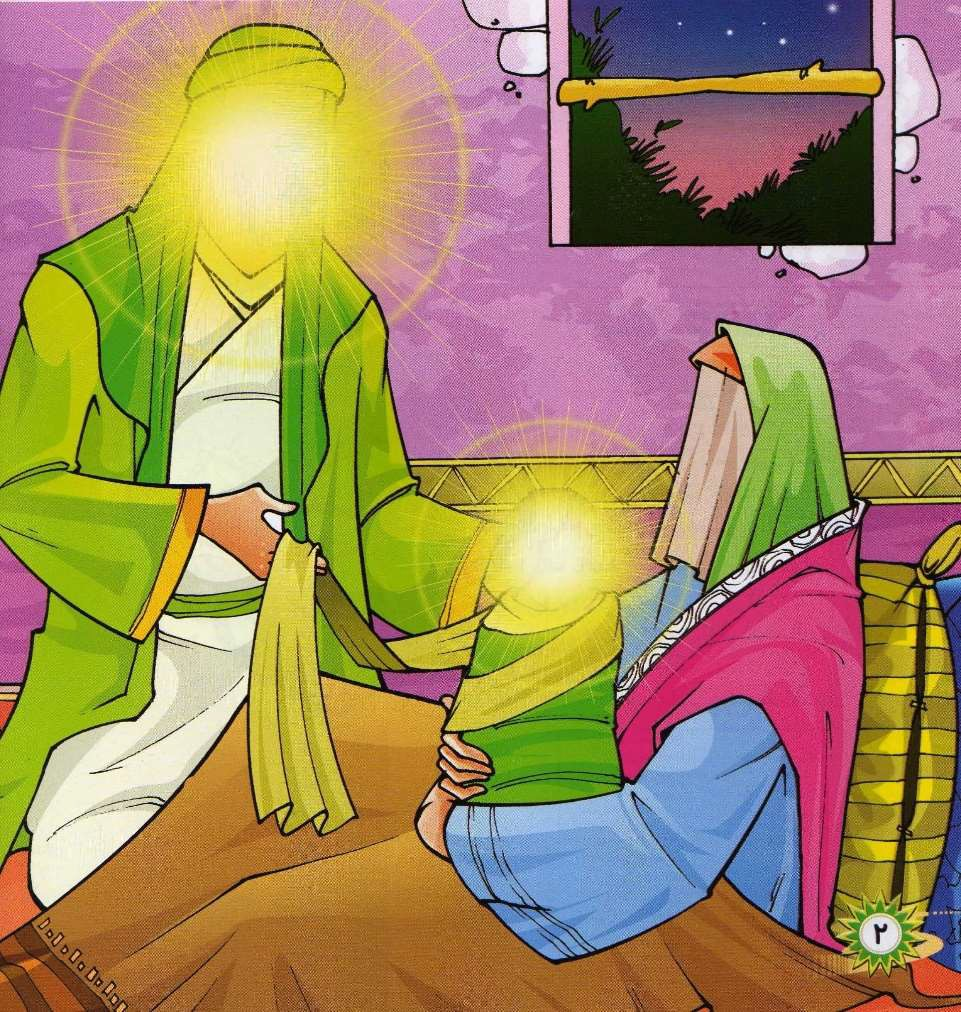
\includegraphics[width=6.3in,height=4.20208in]{media/image4.jpeg}

Selon la théologie musulmane, l'islam est la religion originelle de
l'humanité.VICTOR MOUSSA - STOCK.ADOBE.COM

\subsection{► Que dit la tradition ?}

Selon la théologie musulmane, l'islam est la religion originelle de
l'humanité.~\emph{« Tout homme est né musulman »,}~dit un hadith
attribué
au~\href{https://www.la-croix.com/sacralite-prophete-lislam-2020-11-06-1101123195}{\underline{prophète
Mohammed}}. L'homme est né pour adorer Dieu : certes, il a reçu une
dignité plus haute que les autres créatures, mais celle-ci est
conditionnée à sa soumission au Dieu unique. Plus un homme applique la
loi divine (\emph{charia}), plus il devient humain. Quant au « mécréant
» (\emph{kâfir}), qui refuse de suivre la charia, il se situe en quelque
sorte à un degré inférieur d'humanité.

Cette sévérité envers les non-musulmans s'appuie sur la lecture du texte
coranique qui s'est imposée à partir du IX\textsuperscript{e}~siècle,
lors de la transformation de l'islam en un empire soucieux de se
légitimer. Confortée par des hadiths rédigés à cette époque, elle
dépeint une vérité unique et non négociable. Elle insiste sur les
versets du Coran particulièrement virulents envers les polythéistes,
païens ou idolâtres, qualifiés d'\emph{« associateurs
»}~(\emph{mouchrikoun}) car ils « associent » à Dieu d'autres divinités.

Quant aux athées,~\emph{« ils appartiennent, selon la théologie
musulmane, à une catégorie de mécréance encore inférieure aux
polythéistes, aux juifs et aux chrétiens »,~}explique l'islamologue
Abdessamad Belhaj, chercheur au Centre interdisciplinaire d'études de
l'islam dans le monde contemporain de l'Université catholique de
Louvain. Même si des institutions comme le Haut Conseil des oulémas du
Maroc ou la Maison de la fatwa en Égypte considèrent que les apostats ne
peuvent plus être condamnés à mort, cette peine reste appliquée dans une
dizaine de pays, comme l'Afghanistan ou
la~\href{https://www.la-croix.com/Monde/Afrique/prisons-Mauritanie-calvaire-dun-apostat-2019-09-30-1201051050}{\underline{Mauritanie}}.

\subsection{ Pourquoi juifs et chrétiens bénéficient-ils d'un statut
spécifique ?}

Selon la tradition musulmane, chrétiens et juifs font l'objet d'un
traitement différent des autres non-musulmans : ils bénéficient dans le
droit islamique d'une protection juridique particulière (\emph{dhimma})
toutefois accompagnée d'injonctions humiliantes, comme l'interdiction de
monter à cheval ou de construire des lieux de culte dépassant ceux des
musulmans.
 

\emph{« Le Coran est très ambivalent au sujet des ``gens du Livre''
»,~}rappelle
l'historien~\href{https://www.la-croix.com/Culture/Livres-et-idees/historiens-decryptent-Coran-avant-lislam-2019-11-27-1201063090}{\underline{Guillaume
Dye}}, professeur à l'Université libre de Bruxelles (1). Selon la
sourate 5, juifs et chrétiens ne doivent pas être pris pour~\emph{«
alliés »~}(5, 51) mais, quelques versets plus loin, on lit qu'ils ne
seront~\emph{« point affligés »~}(5, 69). Les chrétiens se voient
reprocher de nier l'unicité de Dieu mais du respect est exprimé pour les
prêtres et les moines, qui~\emph{« ne s'enflent pas d'orgueil ».}

Selon une théologie dite de la falsification (\emph{tahrif}), les juifs
et les chrétiens ont altéré le message transmis par leurs prophètes
respectifs (Moïse, Jésus), message qui n'était autre que l'islam. Le
Coran, lui, corrige cette déviation en transmettant fidèlement le
message révélé à un ultime prophète, Mohammed. À Médine, celui-ci aurait
signé une~\emph{« Constitution »~}disposant que les juifs, notamment,
pouvaient pratiquer leur religion en sécurité, mais ces relations se
sont rapidement détériorées.

\subsection{► Quelles pistes pour une « théologie du pluralisme » ?}

Les attentats visant des « mécréants » en terrasse à Paris, les
persécutions contre les Yézidis ou les chrétiens en Irak, sont autant de
conséquences d'une lecture littéraliste du Coran encouragée par l'essor
du salafisme saoudien à partir des années 1970. D'autres lectures ont
pourtant existé dès les premiers siècles de l'islam. Contrairement à la
doctrine sunnite traditionnelle, l'exégèse rationaliste a par exemple
conclu très tôt à une~\emph{« égalité entre tous les êtres humains, tous
étant dotés de la même raison les rendant aptes à comprendre la parole
de Dieu »,~}rappelle l'islamologue Pierre Lory, directeur d'études à
l'École pratique des hautes études (EPHE).

Pour Abdessamad Belhaj, tout l'enjeu est aujourd'hui de refonder le
rapport à l'altérité sur la base de l'éthique, et de\emph{~« mettre
l'homme au cœur de la théologie »}. Pour cela, certaines valeurs
présentes dans l'islam gagneraient à être redécouvertes, comme celles du
soin, du don et du service à l'humanité, longtemps éclipsées selon lui
par l'autorité et la loyauté à la communauté musulmane ou à la tribu.

(1) Il a codirigé avec Mohammad Ali Amir-Moezzi, Le Coran des
historiens, 2019, Éd. du Cerf, 3~408~p., 89~€.

Faudra-t-il sauver les salafistes ?

Le gouvernement français a voulu lancer en octobre 2019 une offensive
contre l'islamisme et les courants radicaux, rapidement relayée par un
emballement médiatique qui a échappé à tout contrôle. Or, l'ennemi
désigné n'a nullement été identifié selon des termes juridiques, pas
plus que ses torts. On lui reproche sa piété rigoureuse, son voile, sa
pratique du jeûne de Ramadan, sa barbe fournie, son refus de toucher les
femmes, ce qui le rapproche dangereusement de n'importe quel fidèle
conservateur.

L'offensive vise donc une manière de concevoir la piété musulmane, et
nullement une qualification criminelle ou une atteinte à l'ordre public.
C'est dire que nous sommes confrontés à un « délit de sale gueule »,
lequel échappe à la tradition juridique républicaine, délit qui est
indiscernable, sans limite, extensible, mais politiquement pratique
auprès d'une opinion chauffée à blanc par les attentats et
l'immigration.

\subsection{Un engagement d'abord religieux}

Si l'islamiste ainsi décrit ressemble évidemment
au~\href{https://www.la-croix.com/Religion/Islam/Quest-salafisme-2018-10-14-1200975866}{\underline{salafiste}},
c'est oublier un peu vite que l'écrasante majorité des~\emph{salafi~}--
ceux qui sont attachés au modèle des « anciens » (les~\emph{salaf}),
c'est-à-dire les compagnons du Prophète -- se veulent quiétistes : leur
mode d'action est la prédication et l'action missionnaire
(la~\emph{da`wa}). Le salafiste souhaite d'abord vivre un islam épuré et
intégriste -- au sens d'intégral -- dans le cadre de sa famille et de sa
communauté.

Ce mouvement est distinct d'un engagement politique, de sorte que les
salafistes sont rarement liés aux Frères musulmans, qui eux forment un
mouvement politique. Si la matrice religieuse et idéologique du
salafisme imprègne les mentalités djihadistes, elle ne se confond pas
avec celles-ci, ni dans la pensée, ni dans les faits. La radicalisation
concerne donc à des degrés différents et sous des formes incomparables
les sympathisants du salafisme et les partisans du djihadisme de Daech.
Les premiers ont un engagement d'abord religieux, tandis que les autres
sont mus à la fois par la volonté de puissance, des facteurs politiques,
sociaux et religieux.

\subsection{L'autodidacte de l'islam présente plus de risques que le
salafiste}

L'hostilité des salafistes envers les courants djihadistes a été prouvée
à de nombreuses reprises par des déclarations publiques et surtout en
fournissant du renseignement de qualité auprès des services de police.
Le meilleur ennemi du terroriste est souvent le~\emph{salafi}, et
l'autodidacte de l'islam présente plus de risques que le salafiste.

En outre, le salafisme n'a pas été désavoué par les représentants du
culte musulman pour la simple raison que ce courant n'est pas une
idéologie : il faudrait donc lui enlever son~\emph{isme}~final et
l'appeler, selon la tradition religieuse, la~\emph{salafiya~}; il s'agit
d'un vieux courant légitime de l'islam, qui a fourni des générations
d'imams et de lettrés attachés au sens littéral du Coran et de la Sunna.

\subsection{Un « écosystème » étroit mais rassurant}

Il est évident que le salafisme représente une alternative culturelle et
sociale au modèle français, modèle égalitaire, inclusif, ouvert (au
moins en théorie). Les quelques salafi que j'ai connus -- des convertis
à 25 ou 30 \% d'entre eux -- vivaient dans un étroit triangle
géographique. Parce qu'ils souhaitent faire les cinq prières à leur
heure, sans les décaler, et ce dans une salle de prière, ils sont
contraints de vivre et de travailler non loin d'une mosquée. Ils passent
ainsi de leur habitation au lieu de travail et à la salle de prière,
lesquels se situent nécessairement dans un « écosystème » étroit mais
rassurant. Ils ne peuvent guère être exigeants sur le plan
professionnel.

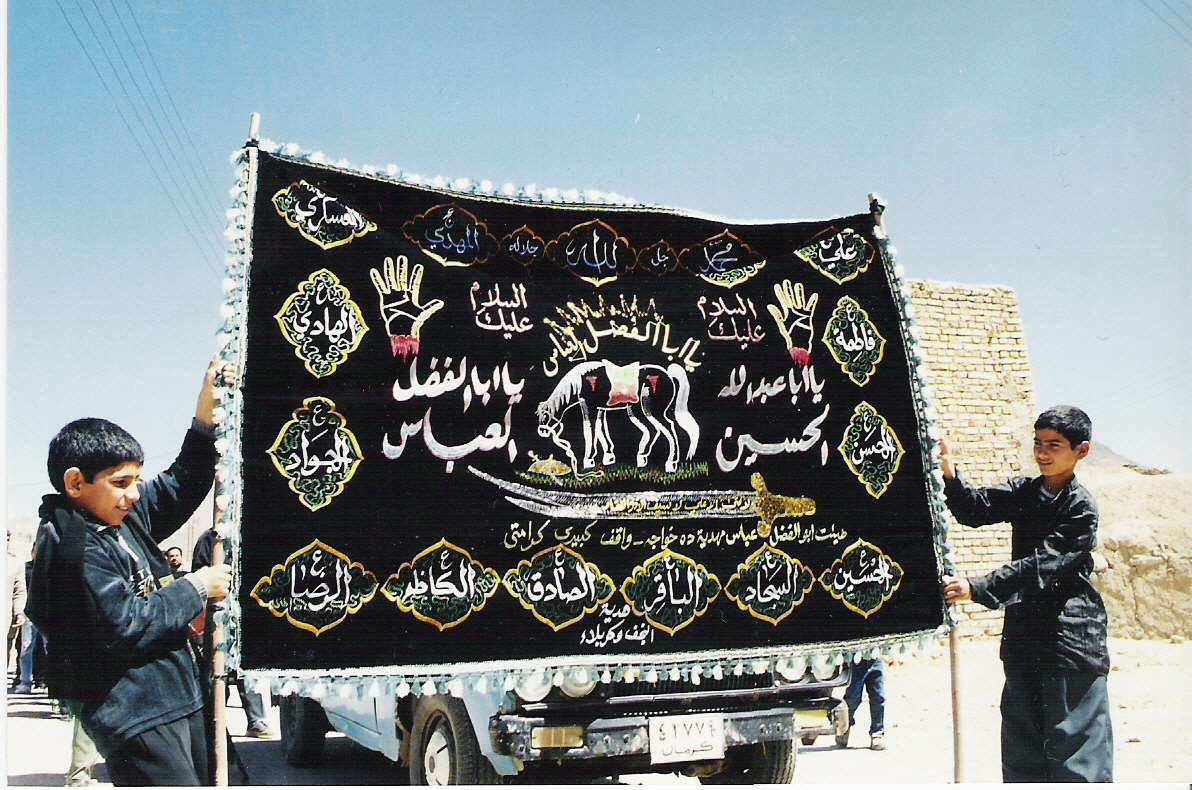
\includegraphics[width=1.97917in,height=1.40972in]{media/image6.jpeg}

\href{https://www.la-croix.com/Religion/Le-Coran-peut-etre-interprete-2021-01-25-1201136852}{Le
Coran peut-il être interprété ?}

Le salafisme, qui représente au moins 40 000 individus, est socialement
dangereux car il impose l'auto-ségrégation, le refus des contacts avec «
ceux qui n'en sont pas ». C'est la raison pour laquelle les spécialistes
des questions de sécurité se refusent à les impliquer dans la lutte
contre le djihadisme. Salafistes et terroristes participeraient à une
même matrice intellectuelle, celle du bien contre le mal, une sorte de
vision sectaire du monde. La différence vient du rapport à la violence :
assumé chez les djihadistes, rejeté chez les salafistes. Leur
fondamentalisme présente l'avantage d'une certaine forme de morale : à
Sartrouville les quartiers salafisés ont vu s'effondrer la toxicomanie
et la délinquance, avec le soutien de la mairie.

\subsection{Confondre l'approche culturelle avec la lutte contre le
terrorisme}

Ces courants ne peuvent être incriminés sur le plan sécuritaire. On
confond donc l'approche culturelle avec la lutte contre le terrorisme. À
moins de changer tout le droit européen, la première doit être menée par
l'éducation, la philosophie, la raison, le débat ; quant à la seconde
elle doit s'appuyer sur le droit et sur des qualifications pénales, et
non sur de vagues impressions de « radicalisation », notion qui n'a
toujours pas été appréhendée de façon rigoureuse en termes sociologiques
et psychologiques.

Comme la guerre d'Algérie nous l'enseigne, une telle manière de
concevoir l'action politique va aboutir à l'effet inverse de celui
recherché : le renforcement de la méfiance collective, le repli
communautaire du côté musulman, l'action violente du côté des « anti »,
et, finalement, la fragmentation sociale et l'insécurité.

\subsection{Islam : les fumées de la radicalisation}

Olivier Hanne, médiéviste (université de Poitiers), chercheur en
islamologie, estime qu'il est très difficile de définir le parcours type
d'une personne radicalisée. Le dernier de trois articles consacrés à
l'islam en France. 
 

Qui parle d'islam aujourd'hui pense aussitôt à la radicalisation. En
2015, on estimait entre 8 000 et 10 000 le nombre de Français
radicalisés. Leurs profils sont si variés qu'il est difficile de donner
des catégories fixes : les mineurs représentent 25 \% des cas, les
femmes 27 \%, les personnes signalées sont plutôt jeunes (entre 16 et 30
ans), leur niveau scolaire est généralement faible, même si l'on
rencontre des diplômés.

La plupart travaillent. Internet représente pour tous ces individus un
passage obligé, même s'il se concrétise différemment : terrain initial
de la radicalisation, facteur de renforcement ou vecteur unique de
l'expression radicale, le partage des contenus djihadistes sur Internet
n'a pas du tout la même fonction chez une adolescente connectée, un
salafiste convaincu et un combattant expérimenté déjà parti en Syrie.

\subsection{Les autorités font feu de tout bois}

De toute évidence, l'attraction pour la radicalité religieuse n'est pas
nécessairement liée à un phénomène de rupture sociale. Les failles de la
société contemporaine (éclatement des familles, déclin des autorités et
des idéologies, chômage, ghettoïsation) créent un terreau facilitateur,
mais nullement déterminant. La frustration individuelle alimente le
recours à des convictions extrêmes, voire le passage à l'acte
terroriste, mais n'est qu'un facteur parmi tant d'autres.

Les autorités font feu de tout bois pour tenter de faire face à une
radicalisation multiforme. En avril 2015, le premier ministre français,
Manuel Valls, annonçait l'ouverture d'une dizaine de centres de
prévention de la radicalisation, dont la plupart furent un échec. Des
sites Internet officiels sont créés et proposent des fiches techniques
contre la radicalisation et le terrorisme, dont le contenu est souvent
simple, voire binaire. Ainsi sur le site
français~\emph{stop-djihadisme.gouv.fr}, un bandeau intitulé «
Radicalisation djihadiste, les premiers signes qui peuvent alerter »
énonce pêle-mêle : « ils se méfient des anciens amis qu'ils considèrent
maintenant comme des impurs » ; « ils changent brutalement leurs
habitudes alimentaires » ; « ils arrêtent d'écouter de la musique car
elle les détourne de leur mission » ; « ils ne regardent plus la
télévision et ne vont plus au cinéma ». Autant de signes extérieurs qui
se rapprochent de l'adolescente anorexique\ldots{} L'efficacité de ces
dispositifs a d'ailleurs été très contestée dès 2015.

\subsection{L'État, tenté d'être omniprésent}

Toute l'entreprise de déradicalisation définit en creux le modèle
positif occidental : monde de loisirs, de consommation, d'épanouissement
personnel et professionnel. Le vocabulaire de la radicalisation masque
le rejet de ce modèle culturel. Et les pouvoirs publics d'hésiter à
appeler leur objectif par son vrai nom : le reconditionnement mental.

Le danger de la déradicalisation se situe dans l'élargissement des
intrusions de l'État : en voulant réinsérer, l'État pénètre dans
l'intimité des individus afin de redéfinir le religieux et lui redonner
une place acceptable. Or, l'État a-t-il compétence pour définir ce
qu'est l'islam, le « bon » islam ? Ne sachant cerner la menace, l'État
est tenté d'être omniprésent, sans en avoir la capacité légale. La
déradicalisation pourrait relever de la posture intellectuelle.

Le problème vient sans doute des hésitations du vocabulaire. Car,
après-tout, qu'est-ce que la radicalisation ? Au
XIX\textsuperscript{e}~le mot anglais~\emph{radical}~était employé pour
désigner les partis politiques britanniques exigeant une réforme
démocratique libérale. Transféré tel quel en France, on l'appliqua aux
partis de gauche, laïques et libéraux qui voulaient réformer la société.

\subsection{Réactions épidermiques}

Le verbe « radicaliser » fut employé régulièrement dans les années
1960-1970 dans une acception politique avec l'idée de « devenir plus
intransigeant, se durcir » ou « plus extrême ». Le premier sens était
donc politique et pas nécessairement négatif. Se déradicaliser était un
synonyme pour « se compromettre ». Appliqué à l'islamisme, le verbe
impose une redéfinition complète des termes : à partir de quand
juge-t-on l'islam intransigeant ou extrême ? par rapport à quelle norme
? à quelle moyenne ?

Les réactions épidermiques qui ont suivi le meurtre de l'enseignant de
Conflans-Sainte-Honorine en octobre 2020 sont tristement révélatrices :
les imams doivent s'exprimer ! les musulmans doivent désavouer le
terrorisme et faire allégeance à la France ! Mais quand ils le font,
c'est encore insuffisant, déloyal et mensonger. Le gouvernement proposa
même qu'ils prient pour la République au cours de la prière collective
du vendredi. Nos références sur la question religieuse restent
tragiquement celles de la Révolution française : comme il y eut les «
prêtres jureurs », adhérant à la loi, contre les « prêtres réfractaires
», obstinés dans leur obéissance à Rome, de la même façon il nous faut
des « imams jureurs », intimement républicains. L'État se retrouve donc
juge des reins et des cœurs.

 
\part{Christologies au défi de la culture pluraliste}
\chapter{Introduction aux Christologies au défi de la culture pluraliste}
\mn{Xavier Gué Cours ISTR 2022-2023}
\section{Synthèse du cours « Christologies et cultures dans l’histoire »}
\subsection{Prolégomènes à une réflexion sur la relation entre les christologies et les cultures et
les religions}

 \begin{Synthesis}
 Prolégomène : 
 \begin{itemize}
     \item  Un écart entre Jésus historique et la possibilité pour nous d'y accéder 
     \item un moment spécifique : la canonisation des Ecritures, reçues par la communauté. 
 \end{itemize}

 \end{Synthesis}

 
\paragraph{Passage}
 Jésus annonce le Règne de Dieu et les premiers disciples annoncent le Christ.

 \paragraph{Mystère pascal} Jésus passe d'un homme singulier au Christ qui est pour tous les hommes, qui est Un avec Dieu. A partir de ce moment là, il devient une bonne nouvelle pour tous les hommes, car il nous permet d'être uni à Dieu et avec tous les hommes.


\paragraph{Comment ?} La transmission du mystère du Christ se joue de manière \textit{vitale} (style de vie des disciples) et en même temps le discours du \textit{discours} (Christologie). Comment le discours sur Jésus va transmettre Jésus dans l'histoire : d'abord les juifs, puis le monde grec, le monde romain,... A chaque fois, des mondes très différents.

\begin{Synthesis}
    Si on affirme que Jésus est pour tous les hommes et tous les temps, il faut qu'on puisse l'annoncer et qu'il soit reçu dans tous les temps et toutes les cultures.
\end{Synthesis}


\paragraph{Christologie doit vérifier l'universalité du Christ} Vérifier : attester. En assumant la \textit{matrice de chaque culture}, le Christ se fera comprendre et recevoir. Rejoindre tous les hommes là où ils sont dans leur culture. 

\paragraph{Une partie résiste} Il s'agit de purifier la culture qui reçoit par le Christ

\paragraph{la Révélation se déploie dans l'histoire par la rencontre avec les Cultures} Tout dialogue transforme. Pas slt un développment organique dans l'histoire mais des influences qui viennent de l'extérieur de l'Eglise. Vincent de Lerins pense une vision organique de l'Eglise mais il y a un échange organique avec l'autre.

\paragraph{la rencontre avec l'autre} a pu développer des hérésies mais aussi développer une théologie féconde, de plus indispensable. 
Règle de discernement et de foi qui permet de vérifier : Calcédoine dit ce qu'on ne peut pas dire. La foi interprétant les Ecritures.

\paragraph{le Christ continue à s'incarner aujourd'hui} la parole de Dieu à s'incarner de nouveau d'une certaine manière. 
 
\subsection{Dimension historique : dans l’histoire des christologies ont émergé par la rencontre
avec des cultures}

\paragraph{Culture juive} un monde qui n'est plus notre monde. Jésus va unifier cette culture par la figure du \textbf{Messie}. cf St Pierre à la Pentecôte. La \textit{Torah} et \textit{l'espérance} sont les deux piliers de la foi juive. Le Messie était attendu. Mais aujourd'hui, est ce qu'on attend le Messie ? Messie ne veut probablement rien dire ? 

\paragraph{de l'intérêt de l'exégèse pour revenir au texte}
\begin{Ex}[Figure du Fils de l'Homme]
Pour les juifs de l'époque, rapport à Dn 7, 13-14, 
\begin{quote}
    13 Je regardais, au cours des visions de la nuit, et je voyais venir, avec les nuées du ciel, comme un \textit{Fils d’homme} ; il parvint jusqu’au Vieillard, et on le fit avancer devant lui.

14 Et il lui fut donné domination, gloire et royauté ; tous les peuples, toutes les nations et les gens de toutes langues le servirent. Sa domination est une domination éternelle, qui ne passera pas, et sa royauté, une royauté qui ne sera pas détruite.
\end{quote}
attente eschatologique (et pas directement Messie).  
\end{Ex}

\paragraph{Culture grecque} Paul rencontre le monde grec paien à Athènes, mais la plupart du temps, il s'adresse par son argumentation à des juifs grecs. 
Comment finalement parler aux grecs ? par le \textbf{logos} et de la \textbf{vérité}. Alors que pour les juifs, on est plus dans la \textit{loi} que la \textit{vérité}. L'innovation, c'est de dire que le \textit{logos s'est fait chair}.

\paragraph{Culture et monde romain} En étudiant Saint Augustin, et le problème de la \textit{religio} qui va être interprété par Lactance et Augustin, d'être relié à Dieu. Jésus va être compris comme \textit{médiateur}. Ces termes existent dans le NT mais on va les mettre en avant. 

\paragraph{Chrétienté} Comment parler du Christ dans un monde chrétien. L'idée de corps social va s'imposer, Eglise comme corps et le Christ comme la tête du Christ, et le Pape vicaire (lieutenant) du Christ. Il faudra christologiser cette idée de Roi en lui apposant le terme de \textit{serviteur}. 

\paragraph{Temps moderne} Prise de conscience en Europe d'une culture qui s'émancipe du Christianisme. Avec deux idées : 
\begin{itemize}
    \item Erasme : l'homme est au centre du monde
    \item L'Europe prend conscience qu'elle peut être moteur de l'histoire : c'est l'homme qui fait l'histoire et non Dieu.
\end{itemize}
La culture sort du Christianisme. Et donc défi pour le Christianisme d'annoncer le mystère du Christ dans cette nouvelle configuration. \textbf{le Christ comme Alpha et Omega de l'histoire, le Christ accomplit l'histoire}. On retourne à l'idée de l'eschatologie. Danielou, de Lubac, Balthazar.

\paragraph{un humanisme qui va se séculariser} L'homme qui accomplit l'humanité (Rahner). Suivre le Christ, ce n'est pas se déshumaniser, c'est s'humaniser, le mystère du Christ révèle le mystère de l'homme.


\section{La christologie au défi de la culture postmoderne et du pluralisme religieux}

 
\subsection{La remise en cause de l’optimisme de la modernité}

L'Eglise Catholique a vu que son rapport au monde avait changé. Il y avait d'autres christianisme (asiatique, arabe). Mais le Christianisme occidental avait pris le \textit{la}. 

\paragraph{On estime l'autre} depuis\textit{ Nostra Aetate}, on regarde l'autre avec estime. \textit{Ad Gentes} et l'interdiction du prosélytisme. 

 \paragraph{les chocs du XX} ont remis en cause le XX.

 \paragraph{les autres religions ne se sont pas écroulées} Au contraire, à la suite de la décolonisation, ces religions sont présentes en Europe. Sur les 18-30 ans, quasiment autant de musulmans (15\%) que de catholiques en France.

 \paragraph{Est ce que les religions sont de fait ou de droit} font elles partie du plan de Dieu ?
\begin{quote}
     « Le pluralisme et les diversités de \textbf{religion}, de couleur, de sexe, de race et de langue sont une
sage volonté divine, par laquelle Dieu a créé les êtres humains. » ? (François - Ahmad Al-
Tayyeb, \textit{La fraternité humaine}, Abou Dabi, 4 février 2019).
\end{quote}
 Ce n'est pas une punition (Babel) : on associait la diversité, à la division et au péché et ici, on l'attache à la sagesse de Dieu.

\paragraph{impact sur la Christologie} On passe dans un monde pluriel, qui resiste. Nous sommes passés de la modernité vers la postmodernité.

\paragraph{C'est quoi la post-modernité ? }
 
\subsection{La culture postmoderne et le pluralisme religieux}

\paragraph{la modernité} le grand récit de la modernité, l'homme se fait tout puissant \textit{à l'image de Dieu}. L'homme participe à la puissance divine.

 
   \begin{quote}
    « C’est\mn{ Rémi Brague, \textit{Le règne de l’homme}. Genèse et échec du projet moderne, Paris, Gallimard, (4ème de couverture).
2015 : } à l’époque moderne que l’homme en est arrivé à se dire le créateur de sa propre
humanité. Autrefois, il se croyait l’oeuvre de la nature ou l’enfant de Dieu. Désormais, il
entend conquérir l’une et s’affranchir de l’autre. Il veut rompre avec le passé, se donner
souverainement sa loi, définir ce qui doit être, dominer. Telle est l’ambition vertigineuse que
raconte cet ouvrage »
\end{quote} 
 
\paragraph{séparation} entre la culture et le religieux. 

\paragraph{Opposition de l'Eglise à cette sortie de la culture}
    Pie IX, dans le syballus (1864), condamnait toute une série d’affirmations dont la dernière :
\begin{quote}

« Le pontife romain peut et doit se réconcilier et composer avec le progrès, le libéralisme et la
culture moderne » (DS 2980). 
\end{quote}


\paragraph{Rupture et continuité de la post modernité par rapport à la modernité} On va critiquer la modernité au nom de la déconstruction des grands récits, y compris celui de la modernité. On arrive à une relativisation, \textit{fragmentation}. 

\paragraph{Il n'y a plus de grands récits, de mythes collectifs}

\paragraph{Neutralité de l'Etat} à la différence de \textit{Cujus Regio Cujus Religio}, ici avec l'Etat laic, diversité religieuse voire culturelle, fragmentation de la vérité. Des cultures qui se confrontent.  La seule unité est le marché, le reste est fragmenté.
\begin{Ex}[Ecologie, dernière utopie]
    Ecologie, un peu ambigue, car un récit par la peur. 
\end{Ex}

\subsection{Un monde déculturé}

\begin{quote}
    Olivier Roy, l'aplatissement du monde, 2022
    Toute culture renvoie à un système d'imaginaires qui fait sens. Un implicite partagé par toute une population. Il note qu'il y a une crise des imaginaires comme la crise des idéologies. 
\end{quote}
 Le politique n'est plus porté par la culture mais par le \textit{contrat}. 

 \paragraph{Les grands récits sont aux mains des radicaux} Sans imaginaire commun, difficile de se projeter dans l'avenir. 

 \paragraph{L'écologie, par un imaginaire mais un } mobilise les jeunes. 

\paragraph{Le marché n'a à faire qu'avec des individus} mais doit lutter contre la culture, les religions : "cela complique tout". On doit supprimer les frontières (globish : langue qui n'est plus culturel mais qui est une langue d'échange).

\paragraph{S'il n'y a plus de cultures, il faut des normes} On est dans l'explicite et pas l'implicite. Ce système normatif doit s'imposer à eux. La pédagogie authoritaire suppose que l'on part d'une \textit{table rase}. \textbf{Epoque de déculturation}.
 
\subsection{Deux principes « unificateurs » de la postmodernité}

\paragraph{Du débat au \textit{dialogue}} Aujourd'hui, il faut apprendre à dialoguer. \mn{cf Synode sur la Synodalité}. L'unité ne peut s'imposer par en haut. Mais on n'a pas la culture du dialogue. On construit notre unité par le dialogue. Il faut passer d'une culture libérale à un imaginaire nourri par le dialogue. 

\paragraph{de l'efficacité à la fécondité} L'unité se fait sur ce qui \textit{marche}. Même si le progrès est remis en cause, on n'est pas loin de la modernité. 
Hannah Arendt : 
\begin{quote}
    on est passé de la vérité au "cela marche".
\end{quote}
\begin{quote}
    « La vérité dont il s’agit dorénavant, c’est celle de ‘l’opérationnel’ (ce qui est faisable : Marchbarkeit). Autrement dit, la vérité à rechercher ne se trouve pas dans l’être ni même dans les événements antérieurs, mais dans la transformation du monde, dans l’organisation du monde ; c’est la vérité qui se rapporte à l’avenir et à l’action » (Ratzinger, La foi chrétienne
hier et aujourd’hui, 25).
\end{quote}
Il faut une vérité \textit{applicable}. 
\begin{quote}
    Paul VI (Evangeli nuntiandi 1975) : « L’homme contemporain écoute plus volontiers les
témoins que les maîtres — disions-Nous récemment à un groupe de laïcs — ou s’il écoute les
maîtres, c’est parce qu’ils sont des témoins ”. »
\end{quote}
Le témoin, c'est celui qui montre que le discours marche dans sa vie. 

Mais l'efficacité (cela marche) ne prend pas en compte le temps. Passer à la fécondité : ce qui porte du fruit par opposition à ce qui est stérile. Il faut viser une certaine fécondité aujourd'hui. 

\begin{Ex}[Eglises africaines]
    marchent car elles proposent la guérison. 
    Approche néanmoins souvent trop individualisme

    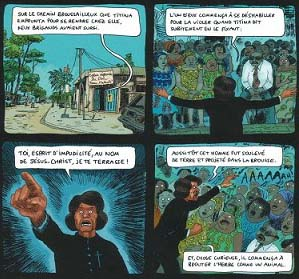
\includegraphics[width=0.7\textwidth]{ChristologiePluraliste/Images/Aya.jpg}
\end{Ex}

\subsection{La christologie à l’épreuve du dialogue}

\paragraph{Remet en cause le Christ comme le tout} Elle reinterpréte la différence entre contingent et absolu, Jésus et le Christ. On a bcp insisté sur \textit{Jésus et l'unique}. Si on annonce Jésus absolu, on ne peut entrer en dialogue. Il convient donc de se reposer la question de décentrer \textit{Jésus} par rapport à \textit{Dieu}. 

\paragraph{comment annoncer le Christ de manière dialogale et rassembler les hommes} question pas simple 
\begin{quote}
    Mgr Ladaria dans la présentation du document de la CTI (dont il est le secrétaire)
Christianisme et les religions 1996 écrit : « En contraste avec l’intention et la lettre même des textes conciliaires, un certain relativisme religieux s’est développé dans certains milieux au cours des années postconciliaires, comme si toutes les religions étaient d’égale valeur pour obtenir le salut; on perdit ainsi grandement le zèle missionnaire, et même la médiation unique
et universelle du Christ fut mise en doute. »
\end{quote}



\subsection{La christologie au défi de la fécondité sociale} 


\paragraph{fécondité} Les fruits de Sainteté. 
\begin{quote}
    Voir les critères de vérité de la Révélation : le GRIC : GROUPE DE RECHERCHE
ISLAMO-CHRETIEN (GRIC), « L’Ecriture des uns vue par la foi des autres », Ces Ecritures
qui nous questionnent, la Bible et le Coran, Le Centurion, Paris, 1987, p. 71-139 (chapitre 3 ).
Outre le contenu du message (du Coran), le Gric propose le critère de la fécondité du message
pour juger de l’authenticité de la révélation coranique. « L’autre critère (…) est celui de la
fécondité du message parmi les hommes (…). On doit donc pouvoir reconnaître dans la vie
individuelle et collective des hommes d’hier et d’aujourd’hui l’influence du message ; ce
qu’on pourrait appeler des fruits de sainteté » (p.103).
\end{quote}

\paragraph{Christologie} dans cette perspective. Quel image d'un Christ qui transforme notre société ? \textbf{des christo-praxies}. Certains auteurs montrent que le Christ doit inspirer notre agir et susciter la fraternité entre nous. Si elle nous enferme sur nous mêmes, il y a un problème.


\section{Plan, bibliographie et déroulement du cours}
\subsection{Plan}
 
\subsection{Bibliographie}
 
\subsection{Déroulement}


 \section{Texte}











 


\chapter{De Jésus au Christ}

\section{Eléments bibliographiques}
\begin{itemize}
    \item HARNACK, A., L’essence du christianisme, tr. par J.-M. TÉTAZ, Genève 2015.
    \item HAZARD, P., La crise de conscience européenne 1680-1715, Paris 1961.
    \item LESSING, G. – REIMARUS, Fragments d’un anonyme de Wolfenbüttel, tr. par M. GÉRAUD,
Paris 2018.
    \item REYMOND, B., A la découverte de Schleiermacher, Paris 2008.
    \item SCHLEIERMACHER, F., Discours sur la religion à ceux de ses contempteurs qui sont des
esprits cultivés, tr. par I. J. ROUGE, Paris 1944
    \item ID., La cohérence de la foi chrétienne, tr. par B. REYMOND, Genève 2018.
    \item SCHWEITZER, A., « Histoire des recherches sur la vie de Jésus. Considération finale », ETR
69 (1994) 153-164 (tr. par J-P. SORG).
\end{itemize}

%--------------------------------------- 
\section{Introduction}

\paragraph{Une culture de dialogue, c'est accepter de se remettre en cause} Sinon, on est dans une \textit{apologie}, une \textit{dispute}. 

\paragraph{Comment comprendre le dogme ?} \textit{Si Jésus est vrai Dieu}, où on accepte ou on accepte pas.  Aussi, il ne faut pas partir du dogme mais les conditions actuelles nous obligent à repartir de Jésus et l'histoire de Jésus comme un lieu de débat. \textit{Qui dites-vous que je suis}. Le recevoir dans le dialogue.

\paragraph{le dogme au service de la parole de Dieu}

\paragraph{Approche du cours, ne pas partir du dogme mais du dialogue sur la personne de Jésus} Dans le XIX, un dialogue entre la culture chrétienne et la culture des lumières : 
\begin{itemize}
    \item Pour sortir du dilemne entre \textit{dogmatisme} et du \textit{rationalisme} (Jésus comme maître de moral), il fallait revenir à l'histoire de Jésus et montrer que Jésus est la source du Christianisme.

    \item Or ce retour à l'histoire concrête (à l'homme Jésus), conduit à une certaine relativisation : \textit{Jésus n'est pas l'unique}
\end{itemize}





%--------------------------------------- 
\section{La remise en cause historique de la foi en Christ}

\paragraph{Approche théologique} C'est toujours intéressant de ne pas affronter la question directement en théologie. Ici, l'astuce du chemin est de montrer comment le \textit{débat} a eu lieu.


\subsection{Le mouvement unitarien à l’origine de la crise du dogme christologique}

\begin{Def}[Unitarien]
mouvement anti-trinitaire, qui insiste sur l'unité de Dieu, qui part d'Italie au XVI. Ils vont en Pologne, Grande Bretagne (Newton) et USA (Jefferson, Dickens).
\end{Def}
On l'appelle aussi le \textit{socinianisme}, de Sozzini (1539-1604). 
Ils vont au delà de la Réforme : 

\begin{quote}
    « Quand au Christ, s’il est fils de Dieu il n’a pas la nature divine, “car cela n’est pas seulement contraire à la droite raison, mais c’est aussi contraire à la Sainte Écriture » (Catéchisme de Rakow, question 72).
\end{quote}

Jésus intercède pour l'homme et il n'est donc pas Dieu. A la différence d'Arius qui considérait Jésus comme première des créatures de Dieu et non pas un homme, ici, Jésus est homme. On fait appel à la raison et l'écriture.

\paragraph{Il fallut répondre à ces unitarien} en repartant des Ecritures.




\subsection{La critique des traditions et des dogmes : la Renaissance et les Lumières} 


\paragraph{La Renaissance revient aux sources} avec l'humanisme (Erasme) et Luther (qui revient aux Ecritures). L'idée est que \textit{l'eau est plus pure à la source}. On remet en cause les traditions entassées.

\paragraph{Les Lumières vont valoriser l'autonomie de la Raison} au lieu de s'appuyer sur l'autorité des autres. Doute méthodique de Descartes.  De plus en plus, on va invoquer les Ecritures contre les dogmes.


\paragraph{L'Ecriture va elle même être fragilisée} Richard Simon, Oratorien (1711) publie \textit{l'histoire critique du vieux testament} (1630). Il s'aperçoit qu'il y a des problèmes, en particulier que Moise ne pouvait avoir écrit le Pentateuque. 





\subsection{La crise du principe scripturaire}  
\paragraph{Question herméneutique au dépend de l'autorité} Chez les catholiques, le magistère.  Mais les protestants, problème du critère (Luther dit : \textit{la Foi sauve}). 

\subsection{La rupture entre la vérité universelle et la révélation historique}  
\paragraph{XVIII : siècle de la Loi} ce qui est stable, découverte avec Newton des lois qui gouvernent le monde. on a du mal à penser l'intervention de Dieu dans le monde. 

\paragraph{Signification universelle de Jésus est posée} Lessing oppose une vérité universelle à un événement historique : 

\begin{quote}
   « Des vérités historiques accidentelles ne peuvent jamais devenir la preuve de vérités rationnelles nécessaires » (Lessing, Über den Beweis des Geistes und der Kraft, 1777). 
\end{quote}

Les vérités sur Dieu sont inaccessibles à un événement historique, fut il Jésus. E. Kant dira que \textit{Jésus c'est celui qui a incarné les valeurs mais quand on a la loi morale, on n'a plus besoin de lui}.

\subsection{La thèse de Reimarus et l’aboutissement christologique de la crise} 

\paragraph{Reimarus pousse à l'extrême} Il est publié à titre postume, avec une intention radicale entre Jésus et les apôtres. 
\mn{LESSING, G. – REIMARUS, Fragments d’un anonyme de Wolfenbüttel, tr. par M. GÉRAUD, Paris 2018.}

A partir de là, il va expliquer ce qui s'est passé (ce sont les apôtres qui fondent le christianisme). Rupture maximale entre Jésus et le Christ de la Foi.

\begin{quote}
    « J’ai montré jusque-là que le nouveau système modifié des apôtres, celui d’un libérateur spirituel souffrant qui doit ressusciter de la mort et après son Ascension au ciel reviendra bientôt du ciel avec une grande force et dans une grande gloire, est inventée et fausse dans son premier fondement essentiel, à savoir la résurrection d’entre les morts : 1) parce que le témoignage prétendument extérieur de la garde romaine, chez Mathieu, est en soi souverainement absurde, et n’est jamais mentionné par aucun des autres évangélistes et apôtres, mais que ce système est contredit par nombre de circonstances, si bien qu’il reste plutôt tout à fait possible et fort vraisemblable (…) que les disciples de Jésus étaient venus la nuit, avaient volé le cadavre et dit ensuite qu’il avait ressuscité ; 2) parce que les disciples de Jésus eux-mêmes, comme témoins de la résurrection, non seulement varient beaucoup sur les points principaux de leur déclaration, mais encore se contredisent aussi entre eux de plusieurs manières, clairement et grossièrement (…) (Reimarus, 105).
\end{quote}


\begin{quote}
    (…) Il ne pouvait manquer que quelques Juifs qui compilaient les différentes descriptions, en viennent à penser que leur Messie viendrait deux fois, et ce sous une forme radicalement différente. On conçoit donc avec évidence que les apôtres se servirent désormais de ce système, bien que peu l’aient adopté, car leur premier système, goûté par la plupart, était réfuté par son issue ; et qu’ils se sont donc aussi promis de Jésus, comme étant le Messie, après sa mort, une autre venue glorieuse. Il faut en outre savoir que les Juifs pensent que la résurrection des morts suivrait l’autre venue du Messie, qui à ce moment jugerait les morts et les vivants : et alors commencerait le royaume des cieux ou l’autre monde (…). Les apôtres devaient donc eux aussi, grâce à leur nouveau système, promettre une autre venue du Christ dans les nuées du ciel, où ce qu’ils avaient maintenant espéré en vain serait exaucé, et où ses adeptes croyants, une fois le tribunal passé, devaient hériter du royaume » (Reimarus, 107).
\end{quote}
%--------------------------------------- 
\section{Retrouver la signification universelle de Jésus}

\paragraph{Comment refaire le lien ? }


\subsection{Schleiermacher : le Christ romantique}  

\paragraph{Courant libéral } au début du XIX. : courant libre par rapport au dogme et le discuter par rapport à la modernité. \textit{Annoncer la Foi dans la culture de l'époque}, c'est prendre des risques, entre répéter et personne ne comprend ou bien s'adapter trop à la culture.

\paragraph{F. Schleiermacher} plus grand théologien du XIX. \textit{Le Christ romantique}. Il est passé par les \textit{frères moraves} (équivalent des charismatiques). En 1799,  il publie le \textit{Discours sur la religion à ceux de ses contempteurs qui sont des esprits cultivés}.
\mn{SCHLEIERMACHER, F., Discours sur la religion à ceux de ses contempteurs qui sont des esprits cultivés, tr. par I. J. ROUGE, Paris 1944}

Il ouvre une nouvelle voie en montrant que l'\textit{homme est essentiellement religieux}. Figure concrète de Jésus et le Christ pour tous les hommes.

\paragraph{L’idée de « sentiment » (Das Gefühl)} Il refuse la métaphysique classique et de l'autre côté la morale (de Kant). Ce qui est premier, c'est l'experience d'une \textit{dépendance radicale avec le divin}. A partir de cette expérience fondamentale, il s'agit de donner des mots à cette expérience spirituelles. Le langage religieux provient de cette expérience mais ne peut l'enfermer.

\begin{Prop}
Est ce que l'expérience mystique est première ou bien est ce que le langage religieux permet de comprendre l'expérience mystique ? 
\end{Prop}

\paragraph{La conscience divine en Jésus} Il y a une conscience divine en Jésus, transparence en Jésus, immédiateté (proximité de Dieu, du Royaume de Dieu).
En Jésus, son humanité possède la capacité de communiquer son expérience aux autres.



\paragraph{Le Christ médiateur et rédempteur} Jésus va révéler à tous les hommes cette dépendance absolue envers Dieu. Un impact collectif sur les hommes, \textit{contagion de son expérience}. 
\begin{Ex}
Quelqu'un qui est lumineux, charismatique, irradie autour de lui, ces disciples deviennent aussi lumineux.
\end{Ex}

\paragraph{le Christ devient le sommet de l'expérience religieuse} Il a eu la foi parfaite et il transmet son expérience. Mais on n'a pas de foi en Jésus, pour Schleiermacher.

Pour la question de la rédemption, la croix n'est pas essentiel pour Schleiermacher. Le Rédempteur c'est celui qui nous met en communication avec Dieu. 





\begin{quote}
    « Il doit, après chacune de ses excursions dans l’Infini, \textit{extérioriser l’impression qu’il en rapporte, de façon à faire d’elle ainsi un objet communicable par l’image ou la parole} (…) et il doit donc aussi, involontairement et pour ainsi dire dans l’état d’enthousiasme\sn{habité par Dieu} (…) figurer pour autrui ce qui lui est arrivé, sous une forme sensible, en poète ou en voyant, en orateur ou en artiste. Un tel homme est un véritable prêtre du Très-Haut, qu’il rend plus accessible à ceux qui ne sont pas habitués à saisir que le fini et sa valeur minime ; il leur présente les choses célestes et éternelles comme des objets de jouissance et de communion, comme la seule source inépuisable de ce vers quoi tend toute leur aspiration supérieure. Il vise ainsi à éveiller le germe somnolent de la meilleure humanité, à allumer l’amour du Très-Haut, à transformer la vie ordinaire en une vie plus haute, à réconcilier les fils de la terre avec le ciel\sn{Ici la rédemption} (…) C’est ici la prêtrise supérieure, celle qui fait connaître l’âme intime de tous les mystères spirituels, et dont la voix descend des hauteurs du royaume de Dieu » (Schleiermacher, Discours, 125-126).
\end{quote}





\paragraph{Les ambiguïtés de la pensée de Schleiermacher} 


\paragraph{Reprend le dogme de Chalcédoine} ce qui fait dire que certains théologiens disent qu'il est tout à fait orthodoxe.

\begin{quote}
    « Quand je considère, dans les descriptions tronquées de sa vie, la sainte figure de celui qui est le sublime auteur de ce qu’il y a jusqu’ici de plus magnifique dans la religion, ce que j’admire ce n’est pas la pureté de sa doctrine morale ; celle-ci n’a fait après tout qu’exprimer ce que tous les hommes parvenus à la conscience de leur nature spirituelle ont de commun avec lui, et à quoi ne peuvent ajouter une plus grande valeur ni le fait de l’exprimer, ni celui d’être le premier à l’exprimer (…). Tout cela n’est que choses humaines. Mais ce qui est véritablement divin, {c’est la magnifique clarté qu’a revêtue dans son âme la grande idée qu’il était venu représenter, l’idée que tout ce qui est fini a besoin, pour sa liaison avec la Divinité, de médiations supérieures.} (…) Considérons seulement la vivante intuition de l’Univers\sn{ie Dieu}, qui remplissait toute son âme, sous la forme parfaite sous laquelle nous la trouvons en lui. Si tout fini, pour ne pas s’éloigner toujours plus de l’Univers et ne pas aller s’éparpillant dans le vide et le néant, pour maintenir sa liaison avec le Tout et s’élever à la conscience de cette liaison, a besoin de la médiation d’un élément supérieur, s’il en est ainsi, cet élément médiateur, qui ne doit pas avoir lui-même à son tour besoin d’une médiation, ne peut absolument pas n’être que fini ; \textbf{il doit appartenir aux deux règnes : il doit participer de la nature divine de même et dans le même sens qu’il participe de la nature finie.} Or, que voyait-il autour de lui qui ne fût fini et soumis au besoin de la médiation ? Et où se trouvait un principe de médiation en dehors de Lui ? Personne ne connaît le Père que le Fils, et celui auquel Il veut le révéler. Cette conscience du caractère unique de sa religiosité, du caractère primordial de sa conception, et de sa force dont celle-ci était douée pour se communiquer et susciter de la religion, a été chez lui à la fois la conscience et de sa fonction médiatrice et de sa divinité » (Schleiermacher, Discours, 316-317).
\end{quote}

\paragraph{Jésus n'est pas un médiateur exclusif pour Schleiermacher} Il ouvre l'idée que la figure du médiateur dépasse la figure historique de Jésus. Médiateur \textit{par excellence} mais non unique.

\begin{quote}
    « Avec cette foi en lui-même, qui peut s’étonner qu’il ait été certain non seulement d’être le médiateur pour beaucoup d’êtres, mais encore de laisser derrière lui une grande école, qui déduirait de sa religion à Lui sa religion à elle, toute semblable (…). Mais \textbf{il n’a jamais affirmé être l’unique objet} de l’application de son idée, être le seul médiateur, et il n’a jamais confondu son école avec sa religion. (…) Aujourd’hui encore il devrait en être ainsi : celui qui pose cette même intuition comme base de sa religion est un chrétien, sans considération d’école, qu’il déduise historiquement sa religion de lui-même ou de n’importe qui d’autre. Le Christ n’a jamais donné les intuitions et les sentiments qu’il pouvait communiquer lui-même comme contenant tout ce que devait embrasser la religion qui devait sortir de son intuition fondamentale ; il a toujours engagé à tenir compte de la vérité qui viendrait après lui » (Discours, 318-319).
\end{quote}

\subsection{La christologie libérale de A. von Harnack (1851-1930)}  
\paragraph{L’essence du christianisme} 
Publication de son cours à Humbold à tous les étudiants de Humbold (Berlin).  
\mn{HARNACK, A. (von), L’Essence du christianisme, tr. par J.-M. TÉTAZ, Genève 2015.
}
On ne peut réduire l'essence du Christianisme aux Evangiles mais aussi à toute l'influence qu'il a eu par la suite. Il faut prendre toute l'histoire. \textit{Pour connaître Jésus, il faut regarder les chrétiens aujourd'hui}.
Plus une personnalité est impressionnante, plus il \textit{impressionne} d'autres et donc c'est en voyant comment les autres ont été touchés, qu'on peut accéder à l'essence de cette personnalité.



\begin{quote}
    « Toute grande personnalité influente ne révèle une partie de son essence qu’en ceux sur lesquels elle agit. On peut même dire que plus une personnalité est impressionnante et plus elle intervient dans la vie intérieure d’autres personnes, moins il possible de reconnaître la
totalité de son essence à ses seules paroles et ses seuls faits et gestes (…) Des forces ont été libérées non une seule fois, mais toujours à nouveau, alors nous devons aussi prendre en compte toutes les productions ultérieures de son esprit. Car ce n’est pas d’une d’ ‘doctrine’ qu’il s’agit, qui aurait été transmise et répétée de façon monotone, ou modifiée arbitrairement, mais bien d’une vie qui, toujours ranimée, brûle de son propre feu » (Harnack, L’essence, 93- 94).
\end{quote}


{Discerner le Christ dans la vie : image du noyau du fruit} Il faut dépouiller le fruit. 

\begin{quote}
    « Dans la prédication de Jésus à propos du Royaume de Dieu, (l’historien) doit séparer ce qui est propre de ce qui est transmis, le noyau de l’écorce (…). Le Royaume de Dieu vient lorsqu’il vient vers les individus, lorsqu’il pénètre dans leur âme et en prend possession. Le Royaume de Dieu est certes domination de Dieu – mais c’est la domination du Dieu saint dans les cœurs des individus, c’est Dieu lui-même avec sa force. Tout drame au sens extérieur du monde, au sens de l’histoire du monde, a disparu ; tout ce qui concernait une expérience future extérieure a été englouti » (Harnack, L’essence, 122).
\end{quote}
\paragraph{La prédication de Jésus} On peut résumer en (p.119):
\begin{itemize}
    \item Le Royaume de Dieu et sa venue
    \item Dieu le Père et la valeur infinie de l’âme humaine
    \item La justice supérieure et le commandement d’amour
\end{itemize}


\paragraph{Le Royaume de Dieu et sa venue} Non pas un royaume exterieur mais un royaume intérieur et individualiste. Il ne s'agit pas de trouver le Règne (pas de dimension sociale). Ce Royaume vient vers les personnes humiliées.




\paragraph{Dieu le Père et la valeur infinie de l’âme humaine}  filiation divine ("inscrit au ciel", "cheveux par terre"). Le Père est la providence : 

\begin{quote}
    « Qui a le droit de dire ‘mon Père’ à l’être qui régit le Ciel et la Terre est lui-même élevé au- dessus du Ciel et de la Terre et possède une valeur qui est plus haute que tout le mystère du monde » (Harnack, L’essence, 129).
\end{quote}

Il ne fait pas la différence entre Jésus et Père et les disciples. L'âme a donc une valeur infinie quand elle se tourne vers Dieu car elle devient "fils bien-aimé". La filiation entre Dieu et Jésus, \textit{unique} et la notre, \textit{adoptive} n'est pas différenciée ici.




\paragraph{La justice supérieure et le commandement d’amour}  

\begin{quote}
    « L’amour du prochain est sur terre la seule façon de mettre en œuvre l’amour de Dieu qui vit dans l’humilité » (Harnack, L’essence, 134).
\end{quote}
Il essaye de dire l'essentiel, le reste est ajouté.

\paragraph{La christologie}   Que devient la christologie ? Quelle auto-compréhension de Jésus ? Pour Harnack, il s'agit uniquement de "garder ses commandements". \textit{Décentrement} de Jésus qui renvoie les disciples au Père. Il va conclure que : 
\begin{quote}
    « Sa conscience d’être le Fils de Dieu n’est donc rien d’autre que la conséquence pratique de la connaissance de Dieu comme le Père et comme son Père (…). Jésus est persuadé de connaître Dieu comme personne ne l’a connu avant lui ; et il sait qu’il a la vocation de communiquer à tous les autres en parole et en acte cette connaissance de Dieu – et donc la filialité divine. » (Harnack, L’essence, 169).
\end{quote}

On retourne ici à Schleiermacher : nous participons comme Jésus, au même niveau que lui.  

Il est en deçà d'une dogmatique classique : 
\begin{quote}
    « Combien s’éloigne-t-on alors de ses idées et des prescriptions lorsqu’on fait précéder l’Evangile d’une confession ‘christologique’ et qu’on enseigne qu’il faut d’abord avoir des idées correctes sur le Christ avant de pouvoir venir à l’Evangile ! C’est inverser l’ordre des choses. On ne peut avoir des idées et des doctrines ‘correctes’ sur le Christ que dans la mesure où l’on a commencé à vivre conformément à son Evangile » (Harnack, L’essence, 181).
\end{quote}

Critique assez forte de la dogmatique.


\subsection{La figure « libérale » de Jésus dissoute par la question eschatologique}  

\paragraph{Découverte récente et renforcement de l'eschatologie} Jésus ne croyait pas à un royaume intérieur :

\begin{quote}
    « Le Jésus de Nazareth, qui vint comme un Messie, qui annonça la moralité du royaume de Dieu, qui fonda le royaume des cieux sur la terre et qui mourut afin de consacrer son œuvre, n’a jamais existé. C’est une figure qui a été esquissée par le rationalisme, rendue vivant par le libéralisme et habillée historiquement par la théologie moderne » (A. \textsc{Schweitzer}, Geschichte der Leben-Jesu-Forschung, 620.)
\end{quote}
%--------------------------------------- 
\section{Conclusion}






 

\chapter{De Jésus au Christ - 2}
\mn{31/1/23}
\section{Eléments bibliographiques}
\begin{itemize}
    \item CHÉNO, R., Dieu au pluriel. Penser les religions, Paris 2017.
    \item COMMISSION THEOLOGIQUE INTERNATIONALE, Le christianisme et les religions, Rome
1997.
    \item DALFERTH, I. U., « Inkarnation : Der Mythos vom inkarnierten Gott » dans Der auferweckte
Gekreuzigte, Tübingen 1994, 1-37.
    \item DUPUIS, J., Vers une théologie chrétienne du pluralisme religieux, tr. par O. PARACHINI,
Paris 1997.
  \item HICK, J., The Myth of God Incarnate, Londres 1977.
  \item KNITTER, P. F., No Other Name ? A Critical Survey of Christian Attitudes Toward the World
Religions, Maryknoll 1985.
  \item KNITTER, P. F., « La théologie catholique des religions à la croisée des chemins », Concilium
203 (1986) 129-138CHÉNO, R., Dieu au pluriel. Penser les religions, Paris 2017.
  \item COMMISSION THEOLOGIQUE INTERNATIONALE, Le christianisme et les religions, Rome
1997.
  \item DALFERTH, I. U., « Inkarnation : Der Mythos vom inkarnierten Gott » dans Der auferweckte
Gekreuzigte, Tübingen 1994, 1-37.
  \item DUPUIS, J., Vers une théologie chrétienne du pluralisme religieux, tr. par O. PARACHINI,
Paris 1997.
  \item HICK, J., The Myth of God Incarnate, Londres 1977.
  \item KNITTER, P. F., No Other Name ? A Critical Survey of Christian Attitudes Toward the World
Religions, Maryknoll 1985.
  \item KNITTER, P. F., « La théologie catholique des religions à la croisée des chemins », Concilium
203 (1986) 129-138
\end{itemize}

%--------------------------------------- 
\section{Introduction}

Un certain nombre de chrétiens ont voulu renouvelé le christianisme à partir de l'histoire. 

Shleiermacher :  Comment finalement des personnes charismatiques peuvent avoir de l'influence ? Mais pas limité au Christ.
Harnack : A partir du moment où l'homme vit de la relation à Dieu, il est messie.
\begin{marginfigure}

\includegraphics[width=\textwidth]{ChristologiePluraliste/Images/TintinFindesTemps.jpg}
\caption{La figure Charismatique peut être un soucis ...}

\end{marginfigure}



%--------------------------------------- 
\section{L’émergence de la théologie du pluralisme religieux}

\begin{Def}[théologie du pluralisme religieux]
modèle du paradigme : à l'image des sciences, on évolue de paradigme en paradigme
\end{Def}

\begin{Ex}
On passe du paradigme ptomélique, à Newton puis relativité.
\end{Ex}

D'après Kuhn, \href{https://fr.wikipedia.org/wiki/La_Structure_des_r%C3%A9volutions_scientifiques}{La Structure des révolutions scientifiques} \mn{intéressant à lire}



%--------------------------------------- 
\subsection{La théorie des trois paradigmes}
  Quel paradigme : 
\begin{itemize}
    \item Vision Exclusiviste, ecclesiocentriste : Le salut pas possible hors de l'Eglise. K. Barth, courant évangéliste actuel (Manille, 1986, "rien ne permet de dire que le salut peut s'obtenir en dehors du Christ confessé explicitement"). \textit{Concile de Florence} au XVI. \textit{Hors de l'Eglise point de salut. }
    \item Vision Inclusiviste, christocentrisme. Au XX. Pas un seul chemin pour aller au Christ.
\item vision théocentrique ou pluraliste. Plusieurs voix pour aller à Dieu
    
\end{itemize}

%--------------------------------------- 
\subsection{Le promoteur du « pluralisme » : J. Hick}

 \paragraph{John Hicks - 2012} D'abord évangélique puis protestantisme libéral après l'Inde. Double conversion. 

%--------------------------------------- 
\subsection{Qui est Paul F. Knitter ?}
 
\paragraph{F. Knitter} Catholique, Chicago, 1966 Rome. Cincinnati. 

1985 : \textit{No Other Name ? } Actes : pas d'autre nom pour être sauvé 


%--------------------------------------- 
\section{La christologie de Knitter : L’unicité relationnelle de Jésus}


\paragraph{Question} comment Jésus est il unique ? 

\paragraph{Histoire} Comment ce Jésus crédible il y a deux mille ans, est il toujours crédible aujourd'hui ? Ce rapport à l'histoire est spécifique aux Occidentaux. Histoire avec un progrès.

\paragraph{Ces approches empêchent le vrai dialogue avec les autres religions} Il faut accepter être impacter à l'autre. Sinon, ce n'est pas un dialogue. Soutient le modèle théocentrique. Jésus : unique mais sans absorber les autre figures prophétiques. 


\paragraph{part des textes bibliques} en même temps historique et théologique


\paragraph{se met à la place des premiers disciples de Jésus} Aspect historique au service de la théologie

%--------------------------------------- 
\section{L’unicité relationnelle de Jésus et la christologie du NT}
%--------------------------------------- 
\subsection{Jésus était théocentrique}
 
 
\paragraph{Jésus est théocentrique} au XX, Jésus annonce le \textit{Royaume de Dieu} : il ne s'annonce pas lui-même. 
Jésus est centré sur le Père. Il est \textit{Regno-centrique} (proche du théocentrisme). 

%--------------------------------------- 
\subsection{Du royaume de Dieu au Fils de Dieu}

 \paragraph{transformation du message du Christ à sa mort}
Dans le NT, il y a un message Christocentrique. Jn 20;28 : "mon Seigneur et mon Dieu". Il y a dejà une subordination du Christ au Père. On pense parfois trop la distinction en pensant au concile de Nicée. 

\paragraph{Jésus aurait fait une expérience de Dieu au début de sa mission} mais cela ne dit pas une exclusivité mais une mission unique. Il s'est pensé le prophète eschatologique de la fin des temps ?  

\paragraph{Loisy} mettait le doigt sur un problème. Expérience de salut faite par ses chrétiens. Les chrétiens ont rencontré Jésus, à la base de cette expérience. 

%--------------------------------------- 
\subsection{La christologie est, depuis le début, dialogique, pluriforme et évolutive.}




 \paragraph{De la diversité des christologies à l’unité de la christologie}
 \paragraph{Revenir à la diversité des christologies}
4 visions de christologie par les chrétiens :

\subparagraph{Christologie Marana tha} contexte apocalytique, jésus vient juger à la fin du temps. Jésus est Seigneur (Mar).
\paragraph{Jésus divin} il est divin dans le sens où il est inspiré par Dieu : \textit{il fait des miracles}. Mais il n'est pas une personne divine au sens ontologique du terme.

\subparagraph{Sagesse ou logos} Jésus est la personnification de la sagesse dont le sens qu'il révèle Dieu.

\paragraph{Théologie pascale} elle n'est pas au centre pour Knitter. Les premiers chrétiens vont diffuser le message. 

%--------------------------------------- 
\section{Unicité et exclusivité du Christ dans le NT}


\paragraph{Pour Knitter, aucune des figures de l'AT n'exprime tout ce qu'est Jésus}
Il a fallu un langage (de l'AT, grec,...) pour dire Jésus. Et donc dialogue.

\paragraph{Cela entraîne une diversité de regards}.

\paragraph{Dimension critique} On va uniformiser ces christologies : on va passer de la vision eschatologique de fils de Dieu (à la fin) à une vision préexistante (le verbe de Dieu s'incarne). Et ceci à la deuxième génération des chrétiens. 



%--------------------------------------- 
\subsection{Le contexte historico-culturel} 


\paragraph{5 pistes d'interprétation des figures du Christ} Il y a dans chaque contexte culturel, on peut utiliser une image un peu différente.

Ce sont des \textit{mythes}, c'est à dire des images et des symboles (cela nous donne un accès) à Jésus. Le mystère du Christ est indéfinissable et donc il ne faut pas absolutiser une image au profit des autres : aucune image ne dit tout. 

\paragraph{Ce qui a été fécond au début, le dialogue, doit continuer aujourd'hui} pour avoir de nouvelles images qui disent Jésus aujourd'hui. Cela a été positif au départ. 

\begin{Synthesis}
Positivité du dialogue avec les religions et la culture au début du christiansime pour dire le Christ.
\end{Synthesis}

\paragraph{Historiciser le langage du Christ} Quand on fait une expérience très forte, on a tendance à dire qu'elle est définitive et exclusive. \mn{Voir discussion avec Charbel attalah : pourquoi les soufis spirituels sont exclusivistes ? }

\paragraph{Statut minoritaire des Juifs dans l'Empire} pour ne pas être absorbé, on utilise un langage de survie, c'est à dire on insiste sur le Christ \textit{définitif}, \textit{insurpassable}.


 
 %--------------------------------------- 
\subsection{« Unique et seul » - les traits du langage confessionnel}


 \paragraph{C'est dans un langage amoureux et enthousiaste} "tu es mon unique". Ce n'est pas un langage métaphysique.   Différent du langage de raison. C'est ainsi qu'il comprend les passages sur "sauveur", "unique".

 

%--------------------------------------- 
\section{La réinterprétation de l’incarnation dans la théologie actuelle}
 

%--------------------------------------- 
\section{La question de la résurrection}


 \paragraph{Sous-estime l'évènement pascal} Dieu intervient dans le monde

 \paragraph{Quand Rahner dit que Jésus accomplit l'homme} pourquoi seulement Jésus serait celui qui accomplit l'homme ? 

 \paragraph{C'est la foi qui est à l'origine de la résurrection} Bultmann. C'est l'expérience des disciples est première. Pour dire qu'il est médiateur, l'expérience des disciples va susciter les récits d'expérience d'apparition pour dire que \textit{Jésus est vivant}.

\begin{quote}
  Jésus est ressuscité dans la Foi des apôtres (Bultmann)  
\end{quote}

 \paragraph{Expérience de Jésus par les disciples toujours essentielle}








 
%--------------------------------------- 
\section{Critique de la proposition de la théologie pluraliste}

\begin{Synthesis}
    Est ce que Jésus témoigne de l'action lui même de Dieu ? Action de Dieu Première ?
    Ou au contraire, expérience religieuse des disciples qui est première.
\end{Synthesis}
 \subsection{Au point de vue philosophique : la question de la vérité}

 \subsection{Au point de vue de l’exégèse biblique et néotestamentaire}
 \subsection{Au point de vue de la théologie et du salut}
  \paragraph{Avec la théologie libérale, d'autres chemins du salut} L'expérience religieuse est absolutisée (l'action de Dieu est secondaire). Alors que pour les Chrétiens, la Foi chrétienne atteste de l'action de Dieu qui ressuscite Jésus d'entre les morts. C'est le \textbf{fondement de notre foi}. 
 \paragraph{Dans la théologie libérale, on confond la révélation de Dieu et la manifestation divine} Pour les Chrétiens, dernière parole de Dieu dans l'histoire. 
La résurrection est la fin de l'histoire : action définitive de Dieu; vision eschatologique. C'est la dernière parole. 
\Chapter{La christologie « pratique » de Theobald}{De Jésus au Christ III}
 

\section{bibliographie}

\begin{itemize}
    \item RICOEUR, P., Amour et justice, Paris 20082.
   \item RICOEUR, P., Soi-même comme un autre, Paris 1990.
   \item THEOBALD, C., « Jésus n’est pas seul. Ouvertures » dans P. GIBERT – C. THEOBALD, Le cas
Jésus Christ. Exégètes, historiens et théologiens en confrontation, Paris 2002, 381-462.
   \item THEOBALD, C., Le christianisme comme style * et **. Une manière de faire de la théologie en
postmodernité, Paris 2007. \cite{theobald_christianisme_2007} 
   \item THEOBALD, C., Selon l’Esprit de sainteté. Genèse d’une théologie systématique, Paris 2015.
   \item THEOBALD, C., « L’unique et ses témoins : jalons pour une théologie de la rencontre entre
juifs, chrétiens et musulmans », Chemins de dialogue 7 (1996), p. 183-202.
\end{itemize}

\section{Introduction}


\paragraph{Approche libérale (et pluraliste) : partent de l'expérience religieuse} alors que notre foi chrétienne a une bipolarité : à la fois l'expérience de Jésus mais \textit{aussi l'expérience historique de la Résurrection de Jésus} : action de Dieu. D'une certaine façon, Dieu répond à Jésus à travers la Résurrection.

\paragraph{On ne peut donc pas partir de l'histoire} On ne part pas ici de Jésus historique mais on part des récits évangéliques, éclairés par la Résurrection, travaillés par elle.


\paragraph{Theobald : part des textes évangéliques} il ne s'agit pas de relativiser le Christ mais que le Christ suscite le dialogue. Il ne déconstruit pas les textes. Et il intègre l'expérience pascale parce que 

\paragraph{Théobald} Jésuite, traduction des oeuvres de Rahner en français. Oeuvre originale. Deux volumes : le Christianisme comme Style. Il essaye de penser le christianisme dans le contexte actuel.


%------------------------------------------------------------
\section{le contexte et le problème}

%------------------------------------------------------------

\subsection{Vivre ensemble dans une société plurielle}

\paragraph{Nécessité de fonder le lien social non sur le religieux mais sur une instance neutre} Pluralité des religions. "Neutralité" du lien social. Comment fait on société alors que nous sommes différents et de culture différente ? Une vraie actualité. 
\begin{quote}
    L’Église « doit désormais proposer la foi au Christ au sein de démocraties pluralistes, prenant donc la mesure de la laïcité de l’Etat moderne et de sa propre position de groupe social parmi d’autres. Précisons brièvement que le pluralisme des ‘convictions axiales’, religieuses ou non, et la cohabitation de leurs organisations dans une même société supposent la forme agnostique du  ‘lien social’ » (style**, 807).
\end{quote}
\begin{Def}[Lien social]
la forme « agnostique » : il s’agit de la neutralité de l’Etat (laïcité). L’Etat est
neutre pour permettre aux différentes traditions religieuses de vivre ensemble.
Lien social : la forme « énigmatique » : l’unité n’est pas disponible, mais elle se fera à la fin
(eschatologie).
\end{Def}
 
\begin{Def}[position agnostique]
  pas lié à une tradition religieuse  
\end{Def}

Il ne faut pas partir de la dogmatique mais éthique

%------------------------------------------------------------
\subsection{Le christianisme n’est plus le ciment de la société}

\paragraph{Nous ne sommes plus en chrétienté} JP II : appelle de ses voeux la \textit{civilisation de l'amour}.

\begin{quote}
    « Une telle situation appelle, selon nous, un déplacement éthique du point de départ de la christologie (...). Les chrétiens (…) doivent montrer qu’ils reconnaissent le caractère énigmatique du lien social, condition d’un véritable pluralisme, non par concession à des pressions externes mais par intime conviction. Or, cette reconnaissance intérieure exige d’eux une véritable reprise christologique » (style**, 808).
\end{quote}


La vision chrétienne cohabite avec d'autres traditions, laic,n Islam...
\begin{Ex}
Historiquement, racine chrétienne de l'Europe.  Mais ce n'est plus la matrice pour comprendre le monde dans lequel on vit.  
\end{Ex}

\paragraph{Christ Roi} 1925- Pie XI. "christologie glorieuse". Dogmatique qui pose aujourd'hui problème.
%------------------------------------------------------------
 \subsection{Le dilemme christologique}
 

\paragraph{soit on continue à affirmer l'unicité du Christ} mais alors comment le Christ peut rassembler le monde. Facteur de division de la société.

\paragraph{Soit on admet d'autres figures religieuses } et alors on relativise le Christ.

\paragraph{Défi qui n'est pas mince} Quel chemin ?

\paragraph{Théobald : l'unicité du Christ fonde un universalisme pluriel} On peut comprendre l'unicité du Christ autrement. 


%--------------------------------------------------
\section{Réflexions sur le Fils « Unique »}
%--------------------------------------------------

Penser son unité avec Dieu et son lien avec tous les hommes. Si on n'insiste que sur l'unité avec Dieu, quelle fraternité avec les hommes ?

%------------------------------------------------------------
\subsection{Le Fils unique et ses frères}

\paragraph{la préférence entraîne la violence}

\begin{quote}
   « L’histoire de Joseph et de ses frères raconte ce qui arrive quand un père préfère un de ses fils à tous les autres : ceux-ci prennent ‘l’Unique’ en haine, ne pouvant plus lui parler amicalement (Gn 37,3s.) » (\citep[p. 821]{theobald_christianisme_2007}.) 
\end{quote}
 
\paragraph{Comment être fils unique d'un père et avoir en même temps des frères ?} il faut penser les deux
\begin{quote}
    « Comment en effet aimer sans privilégier tel ou telle ? Mais préférer quelqu’un, c’est en même temps risquer que jalousie et violence se lèvent à ses et à nos côtés et que la fraternité soit mise à rude épreuve  […] Comment peut-on être ‘fils unique’ d’un Père et avoir en même temps des frères » (Syle**, 821).
\end{quote}

\begin{Prop}
En théologie, penser ensemble ET... ET...
\end{Prop}


\begin{quote}
    « Il nous faut (…) penser ensemble l’une en fonction de l’autre, l’\textit{unicité} de Jésus de Nazareth et la \textit{relation} qu’il entretient avec les siens et, par extension, avec tout être humain. Cela ne va pas de soi dans une tradition théologique qui a fréquemment distingué, voire séparé ces deux facettes d’une seule et même réalité » (Style**, 822).
\end{quote}


\paragraph{Le long parcours de Joseph préfigure Jésus} Élimination de Joseph (puits) et réconciliation. 
\begin{quote}
    « On ne peut être unique que ‘pour’ quelqu’un : Joseph est d’entrée de jeu unique pour Jacob et destiné à le devenir pour ses frères, eux devant entrer à leur tour dans l’expérience de la fraternité ; ce qui nécessite un long parcours qui prend l’allures d’un drame. Jésus est le Fils unique du Père et appelé à devenir l’Unique non seulement pour ses disciples qui reçoivent le nom de ‘frères’ ou d’ ‘amis’, mais encore pour une multitude » (Style**, 822).
\end{quote}


\begin{Synthesis}
Théobald ne part pas du dogme mais de l'éthique / Texte. Interroge les Ecritures et interroge le devenir historique de Jésus.
\end{Synthesis}


%------------------------------------------------------------
\subsection{L’ambivalence de l’unique dans le NT}

Ici, Théobald reprend la distinction de Stanislas Breton\sn{professeur ICP} : \textit{unicité de singularité} (chaque personne est unique) et \textit{unicité d'excellence}(attribué à Jésus dans l'Espace et le Temps) et en ce sens, touche tous les hommes.
\begin{Def}[Unicité de singularité]
 L’unicité de singularité renvoie au caractère unique de toute
personne, à sa singularité : « tout être humain est ‘unique’, au sens où toute rencontre d’autrui
doit surmonter le réflexe de comparaison et aboutir au respect de ce qu’il a d’unique »
\end{Def}
\begin{Def}[    Unicité d’excellence]
  « Le croyant ne doit-il pas accorder à Jésus, outre l’unicité de
singularité qu’il partage avec tout être humain, une ‘excellence’ dans l’espace et le temps ? »
\end{Def}

 




\paragraph{une unicité d'excellence en relation avec les autres} Jésus rentre en relation avec les autres. Théobald part de S. Jean. Tout d'abord le fils unique : 
\begin{Def}[Unicité du Christ]
    cette expression vise à souligner que Jésus est l’unique sauveur de tous
les hommes car il est le « Fils unique » de Dieu. Theobald, néanmoins, développe l’idée que
l’unicité du Christ passe par la reconnaissance de cette unicité par les hommes. L’unicité n’est
pas seulement une qualité métaphysique, mais elle implique une relation réciproque.
\end{Def}
 
\textit{monos} signifie en grec unique mais aussi \textit{seul}. 

\paragraph{Fécondité de l'unique} 
\begin{quote}
    Jn 12,24 : « Le grain de blé tombé en terre, s’il ne meurt pas il reste tout seul (\textit{monos}), vous dis-je, mais s’il meurt il donne beaucoup d’épis ». 
\end{quote}

\begin{quote}
    « La solution de l’ambivalence fondamentale, attachée à toute unicité – lieu où se loge l’ultime tentation de tout homme - , est donc le don de soi, mort du grain pour porter du fruit (…). L’unique n’est donc pas vraiment l’unique, au sens d’une unicité d’excellence, que s’il donne sa vie pour une multitude ; s’il donne sa vie pour que chacun puisse accéder à sa propre unicité » (Le cas, 454).
\end{quote}
Idée que l'unicité de Jésus est une unicité relationnelle : il donne sa vie pour que les autres aient aussi la vie. 

On voit ici comment Théobald relit et reinterprête les écritures avec un regard neuf. 

\begin{Prop}
    Quand on pratique la générosité du samaritain, on participe à l'unicité du Christ. 
\end{Prop}


%------------------------------------------------------------
\subsection{La sainteté et unicité}

Théobald appelle cette singularité, \textit{sainteté}.




\paragraph{Figure du Samaritain et de la démesure qui va jusqu'à aimer sur la croix}
\begin{quote}
    « Celui qui met en jeu son existence au profit du blessé, le Samaritain, devient unique, non seulement pour l’homme rencontré par hasard sur le chemin, mais aussi à ses propres yeux : la démesure de son geste qui défie toute obligation légale s’est avérée à sa mesure, mesure incomparable à celle du voisin » (style**, 827).
\end{quote}

Figure de Jésus. Il y a quelque chose d'excessif. 
Cela est marqué au moment du refus et du rejet qu'il revele qu'il est fils unique : \textit{aimez vos ennemis}. Et cela culmine sur la mort sur la croix. 


%------------------------------------------------------------
\subsection{L’unicité de Jésus et sa manière unique de communiquer la sainteté}


 Ce n'est pas la sainteté qui fait la différence car tout homme est appelé à la \textit{vision béatifique.} Ce qui est unique, c'est qu'il communique de façon unique et définitive de la Sainteté. 
 La sainteté est communiquée \textit{une fois pour toute}\sn{Hebreux}

\begin{quote}
    « Ce n’est donc pas la grâce qui fait la différence entre l’Unique et ses frères humains, ni la sainteté (...). La différence entre Lui et nous consiste seulement dans le fait que c’est Lui, le Fils unique, qui nous communique la sainteté et que c’est en Lui que l’unique promesse de Dieu de nous donner ce qu’il est en Lui-même est devenue dans  notre histoire réalité ‘irrévocable’ » (Style**, 829).
\end{quote}

Cf la distinction que faisaient les Pères de l'Eglise de l'Union hypostatique (en Jésus, les personnes divine et humaine) et l'invitation de Dieu dans les Saints.


\paragraph{Irrévocable} Interprétation de la mort du Christ, sceau de la parole du Christ. 

\paragraph{Comment les approches christologiques présentes doivent être complétées}
%------------------------------------------------------------
\section{Les insuffisances des approches christologiques récentes}
%------------------------------------------------------------

Une théologie, c'est aider les chrétiens à vivre dans un certain contexte. 

\begin{itemize}
    \item Isoler Jésus de ses frères. Seconde Quête
    \item les théologies inclusivistes (Danielou, Rahner), qui insistent sur l'aspect culturel.
\end{itemize}
%------------------------------------------------------------
\subsection{L’unicité de Jésus fondée sur sa relation à Dieu}

\paragraph{Seconde Quête} Käsemann, ... Les disciples de Bultmann qui cherchent le Jésus historique : montrer que Jésus était le seul de son espèce. Montrer que le Jésus de l'histoire et le Christ de la Foi, il y a une continuité. C'était une réponse à Reimarus en montrant qu'en étant historien, il y avait une christologie implicite dans le Jésus historique. 

Techniquement, on avait des critères d'historicité \mn{ex : Jésus discutant avec les pécheurs : on ne faisait pas cela avant ni après}. "Mon Père et votre Père" : distingue bien. "on vous a dit, moi je vous dis" : tous ces motifs qui vont isoler Jésus des autres.

\paragraph{Inconciemment} ces théologies ont mis l'unicité théologique de Jésus au détriment de sa relation avec les hommes.



%------------------------------------------------------------
\subsection{L’unicité de Jésus fondée sur sa dimension eschatologique}

\paragraph{Jésus, un avec les hommes} Rejoint le projet de Théobald de montrer le Christ en Relation. On retrouver cela en G\&S 22 (\textit{Le Christ, homme nouveau})
\begin{quote}
1. En réalité, le mystère de l’homme ne s’éclaire vraiment que dans le mystère du Verbe incarné. Adam, en effet, le premier homme, était la figure de celui qui devait venir, le Christ Seigneur. Nouvel Adam, le Christ, dans la révélation même du mystère du Père et de son amour, manifeste pleinement l’homme à lui-même et lui découvre la sublimité de sa vocation. Il n’est donc pas surprenant que les vérités ci-dessus trouvent en lui leur source et atteignent en lui leur point culminant.
2. « Image du Dieu invisible » (Col 1, 15) , il est l’Homme parfait qui a restauré dans la descendance d’Adam la ressemblance divine, altérée dès le premier péché. Parce qu’en lui la nature humaine a été assumée, non absorbée , par le fait même, cette nature a été élevée en nous aussi à une dignité sans égale. Car, par son incarnation, le Fils de Dieu s’est en quelque sorte uni lui-même à tout homme. Il a travaillé avec des mains d’homme, il a pensé avec une intelligence d’homme, il a agi avec une volonté d’homme, il a aimé avec un cœur d’homme. Né de la Vierge Marie, il est vraiment devenu l’un de nous, en tout semblable à nous, hormis le péché.
3. Agneau innocent, par son sang librement répandu, il nous a mérité la vie ; et, en lui, Dieu nous a réconciliés avec lui-même et entre nous, nous arrachant à l’esclavage du diable et du péché. En sorte que chacun de nous peut dire avec l’Apôtre : le Fils de Dieu « m’a aimé et il s’est livré lui-même pour moi » (Ga 2, 20). En souffrant pour nous, il ne nous a pas simplement donné l’exemple, afin que nous marchions sur ses pas, mais il a ouvert une route nouvelle : si nous la suivons, la vie et la mort deviennent saintes et acquièrent un sens nouveau.
4. Devenu conforme à l’image du Fils, premier-né d’une multitude de frères, le chrétien reçoit « les prémices de l’Esprit » (Rm 8, 23), qui le rendent capable d’accomplir la loi nouvelle de l’amour. Par cet Esprit, « gage de l’héritage » (Ep 1, 14), c’est tout l’homme qui est intérieurement renouvelé, dans l’attente de « la rédemption du corps » (Rm 8, 23) : « Si l’Esprit de celui qui a ressuscité Jésus d’entre les morts demeure en vous, celui qui a ressuscité Jésus Christ d’entre les morts donnera aussi la vie à vos corps mortels, par son Esprit qui habite en vous (Rm 8, 11) [36]. Certes, pour un chrétien, c’est une nécessité et un devoir de combattre le mal au prix de nombreuses tribulations et de subir la mort. Mais, associé au mystère pascal, devenant conforme au Christ dans la mort, fortifié par l’espérance, il va au-devant de la résurrection.
5. Et cela ne vaut pas seulement pour ceux qui croient au Christ, mais bien pour tous les hommes de bonne volonté, dans le cœur desquels, invisiblement, agit la grâce. En effet, puisque le Christ est mort pour tous [39] et que la vocation dernière de l’homme est réellement unique, à savoir divine, nous devons tenir que l’Esprit Saint offre à tous, d’une façon que Dieu connaît, la possibilité d’être associé au mystère pascal.
6. Telle est la qualité et la grandeur du mystère de l’homme, ce mystère que la Révélation chrétienne fait briller aux yeux des croyants. C’est donc par le Christ et dans le Christ que s’éclaire l’énigme de la douleur et de la mort qui, hors de son Évangile, nous écrase. Le Christ est ressuscité ; par sa mort, il a vaincu la mort, et il nous a abondamment donné la vie pour que, devenus fils dans le Fils, nous clamions dans l’Esprit : Abba, Père!
\end{quote}

\paragraph{Une vision une de l'anthropologie} Cela suppose que la vision du monde des Chinois est la même que la vision des Européens. Reste tributaire de la vision universelle des lumières. Il faut parler de plusieurs \textit{universalismes} ou visions du monde : donner un but, une vision du monde. Cela ne veut pas dire que le Concile Vatican II est dépassé : il applique le Concile non pas à la lettre mais comme méthode : \textit{signe des temps } à lire dans la culture actuelle.

Tout en reconnaissant l'intérêt de ces théologies, elles ne peuvent servir de \textit{point de départ}. Partir de l'éthique, pratique, \textit{plus modeste}.

\paragraph{Théologie pratique} qui n'exclue pas la vision théologique ou anthropologique. 


%------------------------------------------------------------
\section{Commencer par une christologie pratique ou éthique}
%------------------------------------------------------------

%------------------------------------------------------------
\subsection{Une nouvelle approche de la christologie}

\paragraph{Normalement, on part de la figure divine de Jésus} Lui propose une autre approche. Ne prennent pas en compte le \textit{chemin } des disciples pour arriver à la Foi, l'unicité relationnelle de Jésus, comme les frères de Joseph. \textit{je suis le Chemin}. Intégrer la genèse de la Foi dans la Christologie même. 
\paragraph{Evangile}
Il s'appuie sur les Evangiles, qui font partie de la Révélation.
Les récits ne nous disent pas qui est Jésus mais ont une pédagogie pour nous faire entrer dans la Foi. \mn{Théobald est Jésuite et les Evangiles ont un goût, histoire}

Il s'agit de faire la même expérience que les disciples :
    
\begin{quote}
    « Le ‘Jésus des historiens’ n’a pas l’actualité et l’autorité nécessaire pour réclamer la foi, c’est-à-dire pour que soient recrées les conditions de la décision jadis appelée par l’évangéliste sur la vérité de ce qu’il appelait la vie ou le royaume » (Le cas 442). Il y a donc une « impossibilité et plus encore une illégitimité de toute communication de la foi par l’histoire » (le Cas 445).
\end{quote}

En lisant Renan, on ne découvre pas la Foi. L'histoire n'est pas là pour accéder à la Foi. Cela peut nous aider à un moment donné. 
\begin{quote}
     Mais ceux-là ont été écrits pour que vous croyiez que Jésus est le Christ, le Fils de Dieu, et pour qu’en croyant, vous ayez la vie en son nom.
    Jn 20,31
\end{quote}


\paragraph{Rencontre de Jésus}
les textes bibliques, pas des textes, mais la parole de Dieu qui nous féconde.
\begin{quote}
    « [La nouveauté du christianisme] ne se réduit pas à l’identité christologique du Nazaréen mais se concentre dans le type de relation qu’il entretient avec ceux qui croisent sa route » (Style*, 57). 
\end{quote}

\paragraph{configuration du récit } Le texte a un effet sur le lecteur : 
\begin{Def}[Configuration]
« Dynamisme intégrateur qui tire une histoire une et complète d’un divers
d’incidents, autant dire transforme ce divers en une histoire une et complète » (Ricoeur,
Temps et Récit II, p. 18). Ici il s’agit de la mise en intrigue, laquelle appartient à la
configuration.
\end{Def}

\begin{Def}[Refiguration]
 
    « J’appelle refiguration l’effet de découverte et de transformation exercé par
le discours sur son auditeur ou son lecteur dans le processus de réception du texte » (Ricoeur,
Amour et justice, 50).
 
\end{Def}
\begin{quote}
    « Comment le soi se comprend-il en se contemplant dans le miroir que lui tend le livre ? » (Ricoeur, Amour et justice, 51). 
\end{quote}
En méditant les Evangiles, on rencontre le Christ. \mn{Arrière fond de Théobald} 



%------------------------------------------------------------
\subsection{Jésus a « impressionné » ses disciples}

\paragraph{Rencontre du Christ : impact, impressionne} La Théologie libérale a insisté sur cette partie. Jésus les a impressionné fortement car il vivait intensément cette relation \mn{Schleiermacher p. XX}

\paragraph{salut lié à la christologie} c'est parce que Jésus est en lien avec tous les hommes qu'il sauve. Et je suis poussé à agir comme lui. Théobald reprend Schleiermacher mais reprend l'Evangile.

%------------------------------------------------------------
\subsection{Le style de vie messianique de Jésus}


\begin{quote}
    Comment caractériser « l’accès à la foi au Christ, compte tenu du point de départ éthique de la christologie, appelé par nos sociétés néo-libérales toujours tentées d’oublier les menaces qui continuent à peser sur le lien social ? On peut, dans la perspective d’une christologie pratique, le définir comme ‘mue d’identité’ qui s’exprime par le passage à un\textit{ style de vie messianique}, à une manière spécifique de se situer dans la société globale » (style**, 813).
\end{quote}

\begin{Def}[Style de vie messianique]
Ce style de vie consiste à vivre l’hospitalité qui suscite la mue
d’identité des personnes rencontrées (par Jésus). « La foi chrétienne n’est pas une doctrine
(…) mais un ‘style de vie’ ou une manière de vivre de la sainteté même de Dieu : seule
l’expérience effective de l’Esprit de sainteté nous permet de confesser et de comprendre un
jour l’indépassable excellence du Fils unique du Père » (L’unique et ses témoins, 19, \cite[p. 794]{theobald_christianisme_2007}).
\end{Def}

\begin{Def}[Mue d’identité]
Le fait que l’autre puisse se découvrir et accéder à son identité singulière.

\end{Def}

\begin{quote}
    « Les évangiles sont en fait des récits de conversion qui ne mettent pas seulement en scène l’itinéraire de Jésus mais aussi et surtout ce qu’il devient en et pour ceux et celles dont l’itinéraire croise le sien : l’accès au Christ se vit comme véritable \textit{mue d’identité} » (style**, 805). 
\end{quote}



\begin{quote}
    Elle engendre l’autre à son identité propre (conversion ?). L’identité d’une personne coïncide
avec l’émergence de la foi (« Ma fille, ta foi t’a sauvée »Mc 5,34), l’autre vit à partir de cette
foi (foi en Dieu), il devient lui-même en se décentrant. Cette conversion consiste à « suivre
Jésus », c’est-à-dire à adopter chacun à sa manière le style de vie messianique\sn{Le regard de Jésus n’est pas évident. « L’adopter effectivement est de l’ordre d’une véritable conversion ou
nécessite une inversion. L’oeuvre messianique consiste précisément dans la victoire sur cet aveuglement » (Style
73). L’incompréhension des disciples montrent bien la difficulté d’adopter l’hospitalité de Jésus (posture
d’apprentissage et dessaisissement de soi). On doit « pouvoir atteindre effectivement l’absence de mensonge ou
la concordance absolue entre pensées, paroles et actes, entre la ‘forme de vie’ de quiconque et son ‘fond’,
concordance, qui, par principe, est chaque fois unique et incomparable » (style 75).}. Jésus devient
l’unique à leurs yeux : c’est-à-dire celui qui leur a communiqué la sainteté. 
\end{quote}

\paragraph{6 étapes}
\begin{itemize}
    \item Apprentissage de Jésus (He 5, 8) dans ses rencontres, il vit la sainteté
    \begin{Def}[Sainteté]
 Capacité d’apprentissage ou dessaisissement de soi au profit d’une présence à
quiconque, ici et maintenant (voir Mc 8,35).
\end{Def}
\item Jésus ne s'impose pas mais permet à l'autre d'accéder à lui -même. Il va libérer l'autre de ses craintes et se dire. 
\item l'émergence de la Foi : quand on accède à son identité, elle commence à être sauvé. Foi en Dieu. cf la Femme adultère, \textit{Ta Foi t'a sauvé}. de l'hospitalité de Jésus arrive la Foi. Il prend des exemples dans l'Evangile : elle libère les personnes rencontrées et les ouvre à une vie nouvelle
\item refiguration, mue d'identité : conversion des personnes qui croisent Jésus, ces gens qui ont changé de vie en rencontrant Jésus. Chacun à adopter le style de vie messianique. Nous avons à devenir hospitalier et leur permettre d'advenir à leur identité.
\item les personnes qui accèdent à cette vie nouvelle \sn{le possédé à Gerasa reste et ne devient pas disciple de Jésus} ne sont pas forcément tous disciples. Mais ces rencontres ne sont pas forcément un changement de vie. Refus. Comment alors maintenir le lien social quand il y a refus de la rencontre ? 
Théobald introduit la règle d'Or.
\end{itemize}
 
\begin{Def}[Concept d’hospitalité ]
Quand l’hospitalité se produit, c’est l’accomplissement des temps
messianiques. Aussi, dans cette expérience de la rencontre avec Jésus, de l’hospitalité de
Jésus est engendrée la foi, le royaume de Dieu advient. « Les aveugles voient ». C’est
pourquoi on peut qualifier de « messianique » le style de vie hospitalier de Jésus car il libère
les gens rencontrés et les engendre à la foi pour une vie nouvelle.
\end{Def}

\begin{Def}[Engendrement]
Il s’agit du devenir « fils de votre Père ». Il a lieu quand on « réalise tout
d’un coup que l’appel démesuré à être connu comme Dieu, dans telle ou telle situation, est
toujours ‘à la mesure’ de chacun » (L’Unique et ses témoins, 200).
Intercommunication : une autre manière de dire le dialogue avec cette nuance où l’on
communique à l’autre sa sainteté.
\end{Def}
%------------------------------------------------------------
\subsection{Le style de vie de Jésus à l’épreuve du refus}

Jésus suscite l'opposition qui l'amènera à la croix. La notion de réciprocité se métamorphose en règle d'amour, de la \textit{mesure} à la \textit{démesure}. \mn{Jn 10, 20 : il déraisonne. }
\begin{quote}
    « Sans le correctif du commandement d’amour (…) la Règle d’Or serait sans cesse tirée dans le sens d’une maxime utilitaire dont la formule serait do ut des, je donne pour que tu donnes. La règle : donne parce qu’il t’a été donné, corrige le afin que de la maxime utilitaire et sauve la Règle d’Or d’une interprétation perverse toujours possible » (Ricoeur, Amour et justice, 39). 
\end{quote}


\begin{Def}[Règle d’or]
 \begin{quote}
     « Tout ce que vous désirez que les autres fassent pour vous, faites-le vous-mêmes
pour eux : voilà la Loi et les Prophètes » (Mt 7,12). 
 \end{quote} Avec Jésus, on passe de la justice
(relation de réciprocité) à l’amour (démesure : l’amour des ennemis) et de l’amour à l’amour
définitif. Jésus accomplit donc la Loi et les Prophètes en accomplissant la règle d’or : il la
réalise définitivement en aimant ses ennemis.
\end{Def}
Mt 7,12 : règle d'or
\begin{quote}
    
\end{quote}

La règle d'or existe dans d'autres cultures \mn{cf  \cite{kung_lethique_2009}}


Paul Ricoeur : sans 
\begin{quote}
    Do ut des : je donne pour que tu donnes. La règle \textit{donne parce qu'il t'a été donné} Sauve la règle d'or de l'utilitarisme (Ricoeur)
\end{quote}


%------------------------------------------------------------
\subsection{La dimension eschatologique du style de vie de Jésus}

\begin{Def}[Style de vie eschatologique]
« Sa sainteté hospitalière [va] jusque dans son ultime
dessaisissement de soi » (style*, 91). L’absence de mesure ou la démesure fait entrer
l’incomparable de Dieu dans l’histoire (voir style*, 95). « Vous serez parfaits comme votre
Père céleste est parfait » (Mt 5,48). En donnant sa vie, son style de vie est donc définitif,
eschatologique. Sa mort ne dit pas seulement l’une fois pour toutes, mais aussi qu’il
transcende le temps et l’espace en s’identifiant à toutes les victimes comme Mt 25 les
présente.
\end{Def}

 En quoi une dimension eschatologique : 


 \begin{quote}
     « Comment la manière d’être du Nazaréen – son type d’hospitalité absolument unique – a pu engendrer, non seulement la confession messianique des premiers chrétiens, mais encore leur perception du caractère définitif et ultime de ce qui est advenu dans leur rencontre avec lui » (Style 86).
 \end{quote}

C'est la mort de Jésus manifestant la perfection de sa sainteté, dessaisi de lui-même, en partant, pour laisser la place même à l'ennemi.
\begin{quote}
    domine jusqu'au coeur des ennemis
\end{quote}

 


\begin{quote}
    « Sa sainteté hospitalière [va] jusque dans son ultime dessaisissement de soi » (style*, 91). L’absence de mesure ou la démesure fait entrer l’incomparable de Dieu dans l’histoire (voir style*, 95). « Vous serez parfaits comme votre Père céleste est parfait » (Mt 5,48).
\end{quote}

\paragraph{il est lui-même le saint} il brise le refus, Temps et Espace. Il donne à celui qui ne peut pas rendre. Quand on donne à un pauvre, il ne peut pas rendre.


%------------------------------------------------------------
\section{Conclusion}


Jésus n'empêche pas le dialogue mais le favorise. 
Style de vie hospitalier, se dessaisissant pour laisser l'autre advenir à lui-même. 


\begin{Synthesis}
    Une approche éthique, pragmatique partant de Jésus. Approche originale et adaptée à notre monde.
\end{Synthesis}


 



 





 




 








\chapter{Du Christ à Jésus I}

\mn{X Gué le 14/02/23}


 \section{Eléments bibliographiques }

 \subsection{les apologistes}
 \begin{itemize}
     \item CLÉMENT D’ALEXANDRIE, Stromates I à V, Sources Chrétiennes, Paris.
     \item FÉDOU, M., La voie du Christ, Genèses de la christologie dans le contexte religieux de
l’Antiquité du IIe siècle au début du IVe siècle, Paris 2006.
     \item IRENÉE DE LYON, Contre les Hérésies. Dénonciation et réfutation de la prétendue gnose au
nom menteur, tr. par A. ROUSSEAU, Paris 19913.
     \item JUSTIN, OEuvres complètes, Paris 1994.
     \item ORIGENE, Traité des principes I, Sources Chrétiennes 252, Paris 1978.
     \item POUDERON, B., Les apologistes grecs du IIe siècle, Paris 2005.
     \item THEOPHILE D’ANTIOCHE, Trois livres à Autolycus, Sources Chrétiennes 20, Paris 1976.
 \end{itemize}

\subsection{les rationalistes}
\begin{itemize}
    \item B. COTTRET, Le Christ des Lumières. Jésus de Newton à Voltaire 1660-1760, Paris 1990.
    \item E. KANT, La religion dans les limites de la simple raison, Paris 2004
    \item X. TILLIETTE, La christologie idéaliste, Paris 1986.
\end{itemize}

% -------------------------------------------------------------------------------
\section{Introduction}


\paragraph{on ne part pas de Jésus historique} mais du Christ et du \textit{Logos}, titre universel. 
On présuppose que le partenaire du dialogue adhère à quelque chose de commun, le \textit{logos}.

\paragraph{Deux exemples dans l'histoire} Pour le dialogue, il faut un point commun. L'idée est plus grande que le concret historique, Jésus. Notre première approche a été de partir de l'histoire et de l'expérience. Ici, on va partir du spirituel et de l'universel. Au Ième siècle et XVIIIè.

\paragraph{faire de la christologie dans un monde pluraliste} Ce n'est pas facile d'entrer dans un autre type de culture.

% -------------------------------------------------------------------------------
\section{Dépasser le langage de la tribu}

Le premier dialogue a été entre les chrétiens juifs et les philosophes grecs. 

 \subsection{Paul à Athènes}

 \paragraph{Un des seuls récits de Paul avec des non-juifs} On ne voit pas trop de dialogues avec des non-juifs. Il reconnait la valeur de la recherche des Athéniens.
\begin{quote}
    
« Le Dieu qui a créé l’univers et tout ce qui s’y trouve (…) donne à tous la vie et le souffle, et
tout le reste (…). A partir d’une seul homme il a créé tous les peuples pour habiter toute la
surface de la terre, il a défini des temps fixes et tracé des limites de l’habitat des hommes ;
c’était pour qu’ils cherchent Dieu ; peut-être pourraient-ils le découvrir en tâtonnant, lui qui,
en réalité, n’est pas loin de chacun de nous car c’est en lui que nous avons la vie, le
mouvement et l’être, comme l’ont dit certains de vos poètes : ‘car nous sommes de sa race’ »
(Ac 17,24-28).
\end{quote}
 L'homme cherche Dieu en tâtonnant mais Dieu n'est pas loin de nous. \textit{colin maillard}. Dieu n'est pas inaccessible à l'homme car par la création, il est proche de tout homme. C'est différent de Rm 1. Le Paul de \textit{Luc} est plus \textit{optimiste} sur la nature humaine. 
 
\paragraph{Epiménide et Aratos} La premiere partie de Ac 17, 28 cite Epiménide et evoque la prière platonicienne. La deuxième partie (nous tirons...), le poête Aratos.
\begin{quote}
    
     il a voulu qu'ils cherchassent le Seigneur, et qu'ils s'efforçassent de le trouver en tâtonnant, bien qu'il ne soit pas loin de chacun de nous, 28car en lui nous avons la vie, le mouvement, et l'être. C'est ce qu'ont dit aussi quelques-uns de vos poètes: De lui nous sommes la race. Ac 17, 27-28
\end{quote}

\subsection{L’idée de Logos dans le NT}

 \paragraph{concentrée dans les écrits johanniques} 5 fois dans le prologue, Jn 1,1. et aussi une référence dans l'Apocalypse Ap 19,3 "Parole de Dieu". AUjourd'hui, on pense que le prologue viendrait d'un développement de la littérature sapientielle, et que le Logos serait la \textit{Sagesse} (Pr 8,22). Le \textit{Logos} participant à la Création.  Mais dans le prologue, une idée aussi d'accomplissement.


 

 
% -------------------------------------------------------------------------------
\section{L’importance de la christologie du logos au début du christianisme}

\paragraph{chez les intellectuels}

 \subsection{La convergence du christianisme et de la philosophie grecque}

 \paragraph{la philosophie grecque est une sagesse} Apprendre à vivre \textit{bien}. 

 \paragraph{les pères apologistes} se sont fait interprètes. Soucis de faire le pont, de dialoguer avec les autres. Recevoir des autres. En réaction avec la religiosité polythéiste, elle définit le Christ comme Logos. Si l'être du monde est apparu dans la figure de Jésus. "vous philosophe, parlez du logos, nous allons vous accompagner du logos tel que nous le connaissons".

 \paragraph{Logos stoicien} raison du monde, une entité bien connue : ce qui fait sortir le monde du chaos en harmonie. Le monde forme un tout cohérent, une unité. de plus, avec l'idée néo-platonicienne du logos, d'intermédiaire entre le \textit{un} et la \textit{multiplicité du monde}. Le Logos est l'émanation du un. Une virtualité de tous les êtres dans le \textit{logos}.

 \paragraph{Jésus est le logos venu dans le monde} donc:
 \begin{itemize}
     \item universel.     \item Lien avec Dieu.     \item Il se manifeste progressivement dans l'histoire. 
 \end{itemize}
 
\subsection{Le Logos un avec le Père, créateur et principe du monde}

 \paragraph{Idée du Logos, un avec Dieu} Théophile d'Antioche, Tatien, vont développer : Dieu est sage; donc il a une pensée, un logos. Et la parole, c'est le logos extériorisé. Au moment où il sort de Dieu, c'est la Création. 
 \begin{quote}
     Dieu dit et le monde est créé.
 \end{quote}

 Tatien : 


 
\begin{quote}
    « Nous ne disons donc pas, comme le pensent les hérétiques, qu’une partie de la substance de
Dieu se soit changée en fils ou que le Fils a été procrée par le Père à partir de rien, c’est-à-dire
en dehors de sa substance, de telle sorte qu’il fut un moment où il n’était pas, mais nous
disons, en supprimant toute signification corporelle, que la Parole et Sagesse est née du Père
invisible et incorporel, sans que rien ne se produise corporellement, comme la volonté
procède de l’intelligence… De même que jamais la lumière n’a pu exister sans son
rayonnement, de même le Fils ne peut être compris sans le Père (…) » (Origène, Traité des
principes, IV, 4, 1)
\end{quote}


\subsection{Universalité du Logos et le thème des «semences du Verbe»}

 \paragraph{Le thème du Logos disséminé : Justin et les autres} Justin, philosophe, converti au Christianisme, meurt martyr en 165 à Rome. Il n'a pas pensé sa conversion comme une rupture mais un accomplissement. 

Une apologie à l'empereur Antonin : 
\begin{quote}
    « Ceux qui ont vécu selon le Logos sont chrétiens, même s’ils ont été tenus pour athées,
comme par exemple, chez les Grecs, Socrate, Héraclite, et d’autres pareils, et, chez les
Barbares, Abraham, Ananias, Azarias, Misaël, Elie et quantité d’autres, dont nous renonçons
pour l’instant à énumérer les oeuvres et les noms (…). Dès lors aussi, ceux qui, parmi les
hommes des temps passés, ont vécu loin du Logos, furent mauvais, ennemis du Christ,
meurtriers de ceux qui vivaient selon le Logos, tandis que ceux qui ont vécu et qui vivent encore selon le Logos sont chrétiens, sans crainte et sans inquiétude » (Justin, \textit{Apologie}, 46,3-
4).
\end{quote}
\begin{Prop}
Pas besoin d'être chrétien pour accueillir le Verbe : Socrate,... sont des chrétiens.
Être Chrétien, c'est suivre la vérité, le \textit{Logos}.
\end{Prop}

\paragraph{Pour Celse, les Chrétiens sont des athées} car déclarent que les idôles sont des faux dieux. 


\paragraph{Toutes les paroles émanent du \textit{Logos}} idée stoicienne, christianisé en un visage, celui de Jésus. 

\paragraph{Influence stoïcienne et originalité chrétienne} 





\begin{quote}
    « Car la pluie de la grâce divine est déversée sur les justes et les injustes ; Dieu est-il le Dieu
des seuls juifs, et non aussi des gentils ? » (…) « Quand je dis : philosophie, je n’entends pas
celle du Portique, ou de Platon, ou d’Epicure, ou d’Aristote. Mais tout ce qui a été dit de bon
dans chacune de ces écoles, et qui nous enseigne la justice accompagnée de connaissance
religieuse, c’est cet ensemble que j’appelle philosophie. » (Clément d’Alexandrie, Stromates
V,3,18, 6-8)
\end{quote}


\subsection{Le Logos et l’histoire} Le problème de ces théologies, c'est de rester théorique. Comment rattacher à l'histoire, \textit{l'économie du Logos}. Dans son apologie, Justin vont se conformer au \textit{Logos tout entier}, le Christ. Clément d'Alexandrie pense l'économie à travers un très beau texte : 



\begin{quote}
    « Avant la venue du Seigneur la philosophie était indispensable aux grecs pour les conduire à
la justice ; maintenant elle devient utile pour les conduire à la vénération de Dieu. Elle sert de
formation préparatoire aux esprits qui veulent gagner leur foi par la démonstration (…). \textbf{Dieu
est la cause de toutes les bonnes choses}, des unes immédiatement et pour elles-mêmes,
comme de l’AT et du NT, des autres par corollaire, comme de la philosophie. Peut-être même
la philosophie a-t-elle été donnée elle aussi comme un bien direct aux Grecs, avant que le
Seigneur eût élargi son appel jusqu’à eux : car elle faisait leur éducation, tout comme la Loi
celle des juifs, pour aller au Christ. La philosophie est un travail préparatoire ; elle ouvre la
route à celui que le Christ rend ensuite parfait (…). Il n’y a, certes, qu’une route de la vérité,
mais elle est comme un fleuve intarissable, vers lequel débouchent les autres cours d’eau
venus d’une peu partout » (Clément d’Alexandrie, Stromates I, 5,1-3).
\end{quote}

\paragraph{hypothèse de la philosophie comme don de Dieu}
 La philosophie comme don du Dieu \textit{car elles faisaient leur éducation} : parallèle avec la Torah. La route de la vérité, c'est le Christ, grand fleuve, où se rejoignent d'autres courants. 

 Jacques Dupuis : la philosophie est une lampe.\sn{théologie du pluralisme}. Des théophanies dans le cas où elles sont des logophanies. \textit{L'ange du Seigneur à Mambré}, c'est le Logos.
 On voit Adam et le Christ avec Adam.

\begin{figure}
    \centering
    \includegraphics{}
    \caption{le Christ et Adam}
    \label{fig:my_label}
\end{figure}


\paragraph{Mais alors le statut de la philosophie après Jésus-Christ}
 \begin{quote}
    « Si (…) la venue du Roi est annoncée par avance par les serviteurs que l’on envoie, c’est
pour la préparation de ceux qui auront à accueillir leur Seigneur. Mais lorsque le Roi est
arrivé, que ses sujets ont été remplis de la joie annoncée, qu’ils ont reçu de lui la liberté, qu’ils
ont bénéficié de sa vue, entendu ses paroles et joui de ses dons, alors du moins pour les gens
sensés, ne se pose plus la question de savoir ce que le Roi a apporté de nouveau par rapport à
ceux qui annoncèrent sa venue » (Irénée, Contre les hérésies VI, 34, 1).
\end{quote}


 
\subsection{L’identification problématique du Logos avec Jésus Christ} Ils se fondent sur l'histoire, sur le prologue. Et pourtant, le succès du Logos tend à mettre entre parenthèse le Jésus historique et son discours. Un peu trop philosophique.
Bernard Poudron, spécialiste des apologistes : 
 \begin{quote}
    La théologie « trinitaire » […] des apologistes est en réalité essentiellement une théologie du
Logos. Il est en effet remarquable que la plupart des apologistes ne mentionnent pas Jésus ou
le Christ en tant que personnage historique, mais n’évoquent le Fils qu’en tant qu’il est le
Logos de Dieu. » (Pouderon, Les apologistes, 91)
\end{quote}
Cela reste de l'ordre du principe philosophique.



% -------------------------------------------------------------------------------
\section{ La christologie rationaliste dans un dialogue avec l’homme des Lumières}
 \subsection{Les Lumières : de la révélation historique à la révélation naturelle}
 
\subsection{Le Christ comme le grand législateur}
 
\subsection{Le christianisme est aussi vieux que la création}
 
\subsection{Le Christ rationaliste d’E. Kant}
 
% -------------------------------------------------------------------------------
\section{Conclusion}


\section{Textes}





\begin{quote}
    « Dieu engendra son Logos, qui était immanent (endiatheton) en son sein, et le produisit avec
sa Sagesse avant toute chose. Il eut ce Logos comme ministre de toutes ses oeuvres, et par lui
tout a été fait. On l’appelle Principe, parce qu’il est le Principe et le maître de tout ce qui a été
créé par lui. C’est lui, Esprit de Dieu, Principe et Sagesse et Force du Très-Haut, qui
descendait sur les prophètes (…) » (Théophile d’Antioche, A Autolycus, II, 10)
\end{quote}


\begin{quote}
    « Avant que rien ne fût, [Dieu] tenait conseil avec [son Logos] lui qui est son intelligence et
son sentiment. Et quand Dieu décida de faire tout ce qu’il avait délibéré, il engendra son
Logos au-dehors (egennèsen prophorikon), premier-né de toute créature, sans être privé luimême
du Logos, mais ayant engendré le Logos et s’entretenant toujours avec son Logos. »
(Théophile d’Antioche, A Autolycus, II, 22)
\end{quote}



 










\begin{quote}
    « Le christianisme, tel que le présente l’évangile, contient un système religieux qui est non
seulement complet mais encore totalement dénué d’affectation. Il s’agit en réalité du système
de la religion naturelle qui aurait dû continuer sa course, pour le plus grand bien de
l’humanité, s’il avait été propagé avec la même simplicité que celle que le Christ avait utilisée
pour l’enseigner » (Bolingbroke, Philosophical Works, Genève 1968, t II, 322 cité par Cottret,
159).
\end{quote}

\begin{quote}
« Jésus, comme Socrate, avait découvert la religion naturelle ; comme Socrate enfin, Jésus a
été trahi. Socrate et Jésus ne nous sont connus qu’au travers du témoignage suspect de Platon
et de saint Paul. (…) L’Église (…) constitue en fait une sorte d’écran entre le Christ et nous :
‘l’Evangile du Christ est une chose, l’Evangile de saint Paul, et de tous ceux qui se sont
greffés sur la même souche après lui, en est une autre’ (Bolingbroke, Philosophical Works,
Genève 1968, t II, 328 cité par Cottret 160). »
    
\end{quote}


\begin{quote}
«S’il y avait un système moral complet dans l’évangile, nous pourrions nous attendre à le
trouver dans les chapitres V, VI et VII de saint Matthieu dans la mesure où ils contiennent un
sermon prononcée par le Christ en personne et qui ne porte pas sur quelque point particulier
de doctrine, mais sur les devoirs de l’homme. Qu’y trouvons-nous ? De nombreux préceptes
moraux, sans doute excellents, mêlés de toutes sortes des considérations, provenant de
révélations personnelles, et pourtant conformes à ce que la loi de nature commande ou
prescrit, comme le démontre l’exemple des philosophes et des autres hommes de bien parmi
les païens » (Bolingbroke, Philosophical Works, Genève 1968, t II, 3 306-307 cité par Cottret
160).
    
\end{quote}


\begin{quote}
« Quelle place laisser au mystère qui environne le crucifié ? Une certaine révolte se fait jour :
comment les chrétiens ont-ils pu parler au sujet de la mort de Jésus de sacrifice voulu par
Dieu ? » (Cottret, 161). « Imaginons un grand Prince qui gouvernerait un méchant peuple de
rebelles. Alors qu’il pourrait punir ses sujets, il choisit de leur pardonner. Mais il ordonne que
son Fils unique, son Fils bien-aimé, soit mis à mort pour expier leurs péchés et pour satisfaire
son royal courroux. Une telle action paraît-elle bonne, juste ou sage aux yeux de la raison ou à
la lumière de la nature, dénuée de tous préjugées ? » (Bolingbroke, Philosophical Works,
Genève 1968, t IV, 270-271 cité par Cottret 162).
    
\end{quote}


\begin{quote}

   « Nous élever à cet idéal de perfection morale c’est-à-dire à l’archétype de l’intention morale
dans toute sa pureté, voilà le devoir général de l’humanité et cette Idée même qui nous est
proposée comme modèle à atteindre par la raison, peut nous en donner la force. Or,
précisément parce que nous n’en sommes pas les auteurs et qu’elle a pris place en l’homme
sans que nous comprenions comment la nature humaine a seulement pu être susceptible de
l’accueillir, il vaut mieux dire : que cet archétype est descendu du ciel vers nous, qu’il a
revêtu l’humanité […]. » E. KANT, La religion dans les limites de la simple raison, Paris
2004, 134. 
\end{quote}


\begin{quote}
« Si donc un tel homme, d’intentions vraiment divines, était à une certaine époque en quelque
sorte descendu du ciel sur la terre, donnant par sa doctrine, sa conduite, et ses souffrances
l’exemple d’un homme en soi agréable à Dieu, autant, bien entendu, qu’on peut le demander à
une expérience externe (l’archétype cependant d’un tel homme ne devant être recherché nulle
part ailleurs que dans notre raison), s’il avait par tout cela produit dans le monde un bien
moral immensément grand par le moyen d’une révolution dans le genre humain, il n’y aurait
pas lieu néanmoins de voir en lui autre chose qu’un homme engendré naturellement […]. » E.
KANT, La religion dans les limites de la simple raison, 137
    
\end{quote}


\begin{quote}
« L’histoire de l’Évangile est au fond l’histoire de la nature humaine ramenée à une
conception idéale ; elle nous montre dans un individu ce que l’homme doit être, ce qu’il peut
véritablement devenir en s’unissant à lui et en suivant sa doctrine et son exemple. » D. F.
STRAUSS, La vie de Jésus, Paris 1858, 692.
    
\end{quote}


\begin{quote}

    
\end{quote}
\chapter{Du Christ à Jésus II
L’approche de Panikkar
}

\mn{Christologies au défi de la culture pluraliste}

\section{Eléments bibliographiques :}

\begin{itemize}
    \item DUPUIS, J. Vers une théologie chrétienne du
pluralisme religieux, tr. par O. PARACHINI,
Paris 1997.
    \item PANIKKAR, R., Le Christ et l’hindouisme. Une présence cachée, Paris 1972
    \item PANIKKAR, R., Entre Dieu et le cosmos. Entretiens avec G. JARCZYK, Paris 20122.
    \item PANIKKAR, R., OEuvres VIII. Vision trinitaire et cosmothéandrique : Dieu-Homme-Cosmos, tr.
par M. BACCELLI, Paris 2013.
\end{itemize}

\section{Introduction}


\paragraph{Raymond Pannikar et son dialogue avec l'hindouisme} pas très bien vu. 
Ce que dit Jacques Dupuis de Pannikar : 
\begin{itemize}
    \item Commence \textit{inclusiviste} à la façon de Rahner et Danielou
    \item va devenir pluraliste : faire droit aux autres traditions.
\end{itemize}
\begin{quote}
    Dans les autres traditions, ... il est caché.
  
\end{quote}


  
\section{Au-delà d’une théorie de l’accomplissement : Le Christ inconnu
}

%---------------------------------------------------
\subsection{Le Christ est présent dans les autres religions comme un principe caché}

  En 1964, il publie un livre \textit{le christ inconnu de l'hindouisme} :
  \begin{quote}
      Il y a une présence vivante du Christ dans l'hindouisme.
  \end{quote}

  Il dépasse Danielou et de Lubac(théories de l'accomplissement\sn{Les autres religions comme préparation}). Le Christ n'est pas que le \textit{but ontologique} mais il en est l'instigateur, l'origine. 


  \paragraph{le Christ appartient aussi aux autres religions} Il va plus loin que les \textit{semences du Christ} : c'est vraiment lui mais de façon cachée.

\paragraph{premier Pannikar : besoin d'une purification, une \textit{Pâques} pour l'hindouisme} On retrouve dans \textit{Ad Gentes}, \textit{Lumen Gentium}. "il faut que l'hindouisme devienne encore plus hindouisme" et s'approfondir. 


\paragraph{Dans le Christianisme, le Christ est visible} Dans l'hindouisme, besoin d'un dévoilement. 


%---------------------------------------------------
\subsection{La réalité inconnue à la base de toutes les religions} 


\paragraph{Une réalité inconnue, le mystère}

\paragraph{les chrétiens appellent cette réalité inconnue, le Christ} On peut avoir d'autres noms pour nommer ce mystère. Cela l'éloigne de la figure concrète de Jésus. 



%---------------------------------------------------
\section{La vision de la réalité (ou du mystère) selon Panikkar}


%---------------------------------------------------
\subsection{Le contexte vital}

\paragraph{Importance du contexte} Pannikar est d'abord un intellectuel. Né à Barcelone en 1918, mort en 2010 à catalogne. Mère espagnole et Catholique, Père indien et hindou. opus Dei. 
Thèse entre St Thomas d'Aquin et avec un auteur hindou.
Il rencontre l'hindouisme. Je suis parti Chrétien, me suis découvert hindou, mais j'ai trouvé le bouddhisme sans jamais renoncer au Christianisme.

\paragraph{Va quitter l'opus Dei en 1962} Habite près du Gange. Rencontre Jules Montchanin et Henri Lesseau. Va dans leur ashram.


%---------------------------------------------------

 
%---------------------------------------------------
\subsection{L’aporie des visions moniste et dualiste de la réalité}

\paragraph{Principe hindou} Rejete monisme et dualiste. 


\begin{Def}[monisme]
Système qui considère l'ensemble des choses comme réductible à un seul principe  
\end{Def}
\begin{Ex}
Hegel, Spinoza
Stoisme
Harmonie. 
\end{Ex}
 \begin{Def}[Dualisme]
 
 Doctrine ou système qui admet la coexistence de deux principes irréductibles.
\end{Def}
\begin{Ex}
    Gnose, Islam, Christianisme.
    opposition monde spi et matériel.
    Souvent lié au mal : je dois m'en libérer.
\end{Ex}

\begin{Prop}
Aporie du dualisme et monisme.
\end{Prop}

\paragraph{Vision très juste que notre théologie est faite de tensions et paradoxes}
\begin{quote}
    « Si nous visons l’unité (…), à la longue la pluralité, réduite à l’irréel, se rebelle et fait valoir
ses droits. Si nous visons la pluralité (…), c’est la lutte de tous contre tous et la destruction
réciproque » (Panikkar, Vision trinitaire, 233).
\end{quote}
On ne peut tomber dans l'un des pôles, qui sont comme anarchie et dictature. On est tendu entre les deux.


    
\begin{quote}
« La vision a-dualiste affirme : ni Un ni Multiple, parce que la réalité ne se soumet pas aux 
exigences de l’esprit et résout le dilemme en le niant parce qu’il n’y a pas l’Un sans la 
Multiplicité ni la Multiplicité sans l’Un, puisque la réalité est pure relation et que la polarité 
est ce qui la caractérise » (Panikkar, Vision trinitaire, 241).

\end{quote}

\paragraph{Cosmo théandrique} Nouveau chemin. L'idée commune, chez les chrétiens, c'est la Trinité et dans l'hindouisme, l' \href{https://fr.wikipedia.org/wiki/Adva%C3%AFta_v%C3%A9danta}{adveita}. 

%---------------------------------------------------
\subsection{La voie indienne : « la vision a-dualiste » rejoint la voie chrétienne : « la vision
trinitaire »}


 \paragraph{Kasper} POur qu'il y ait une multiplicité, il faut qu'il y ait un. 
 \begin{Ex}
     Pour se compter, il faut d'abord une unité, savoir ce qu'est l'être humain.
 \end{Ex}

 \paragraph{il ne faut pas diviser} Trois niveaux : 

 \begin{quote}
« Cette vision nous dit que la réalité n’est formée ni d’un bloc unique indistinct (…) ni de trois 
blocs ou d’un monde à trois niveaux – le monde de Dieu (ou de la Transcendance), le monde des 
hommes (ou de la Conscience) et le monde physique (ou de la Matière), comme s’il s’agissait d’un 
édifice à trois étages. La réalité est constituée par les trois dimensions en relation l’une avec 
l’autre – la perichorèsis trinitaire, de sorte que non seulement l’un n’existe pas sans l’autre, 
mais que toutes sont tressées, inter-dépendamment. Pris séparément, ou en soi, sans relation avec 
les autres dimensions de la réalité, Dieu, le monde et l’homme sont de simples abstractions de 
notre esprit » (Panikkar, Vision trinitaire, 16).

\end{quote}

\begin{Def}[périchorèse]
    Icone de Roublev de la Trinité, vitalité interrelationnelle.
    Circumcession. "Le père n'est père que parce qu'il a un fils..."
\end{Def}

\begin{Prop}
    Il parle de danse pour parler de périchorèse
\end{Prop}

\paragraph{vision cosmothéandrique} indéchirable. 


\begin{quote}
« Tout est intégré, assumé, transfiguré. Rien n’est envoyé dans le futur : la présence tout entière 
est ici (…). Rien n’est laissé de côté ou considéré comme non rachetable, y compris le corps et la 
mémoire humaine. La transfiguration n’est pas la vision d’une réalité plus belle ni une évasion sur 
un plan plus élevé : elle est l’intuition totalement intégrée du tissu sans coutures de la réalité 
tout entière » (Panikkar, Vision trinitaire, 225).
\end{quote}

\paragraph{La réalité ultime est trinitaire} Dieu / Cosmos / Homme. Réalité supérieure : divine, Homme : conscience. Cosmos : matériel. 


\begin{quote}
    
« Nous ne sommes jamais en dehors de la Trinité. Il n’y a rien en dehors de ce qu’on appelle Dieu 
ou, le divin (…) La réalité ultime est trinitaire : elle est divine, humaine et cosmique. C’est en 
cela même que consiste l’intuition cosmothéandrique. (…). Cosmothéandrique serait donc cette 
vision, cette expérience, de ce que nous sommes une partie de la Trinité, et qu’il y a trois 
dimensions du réel : une dimension d’infini et de liberté que nous appelons divine ; une dimension 
de conscience, que nous appelons humaine  et une dimension corporelle ou matérielle que nous 
appelons le cosmos » (Panikkar, Entre Dieu et le cosmos, 135).

\end{quote}

\paragraph{S'opposer au concept} qui casse les liens. 

\paragraph{Voie de Salut} Aspect gnostique : prise de conscience de l'origine, alors chemin de salut.

\begin{quote}
    
« Tout a la même origine ; tout est en relation ; l’univers tout entier est une famille, un macro- 
organisme : des liens de ‘sang’, pour ainsi dire, animent tout ce qui est. Nous sommes de la même 
race \sn{St Paul à l'areopage}. Nous sommes les membres démembrés de son Corps. Notre devoir (…), c’est de \textit{re-member}\sn{Sic} le Corps 
démembré, de le recomposer, c’est-à-dire de guérir et d’intégrer tous les membres disjoints de la 
réalité, éparpillés à travers espace et temps. L’énergie pour atteindre ce ‘salut’ peut venir de 
plusieurs directions, mais elle n’a qu’une seule source. Et c’est l’aventure de toute la réalité » 
(Panikkar, Vision trinitaire, 251).
\end{quote}

Influence de Teilhard de Chardin ?

%---------------------------------------------------
\section{La christologie de Panikkar : l’interprétation du Christ dans la vision
cosmothéandrique de la réalité} 
%---------------------------------------------------
Une réalité cosmothéandrique : Pour nous Chrétien, un symbole, le Christ, sa manifestation concrête, c'est Jésus.
%---------------------------------------------------
\subsection{Le Christ comme le symbole de la réalité humano-divino-cosmique}

Le Christ est le révélateur. Pannikar dit qu'il est révélateur de la Trinité, alors qu'il révèle le Père. 
\paragraph{Création} La création est pour lui, la réalité ultime. Pour Pannikar, la Création est présentée dans le \textit{Prologue de Jean}. Le Logos s'est incarné depuis le commencement. 



\begin{quote}
    
« Le Dieu créateur doit être interprété, non tel qu’il figure au début de la Genèse, mais tel que 
le présente saint Jean lorsqu’il dit du Verbe de Dieu que ‘toutes choses ont été faites par lui’ 
(Jn 1,3), il est clair […] que le Logos est incarné depuis le commencement, bien que dans
l’histoire il n’apparaisse qu’à la plénitude des temps. D’après la tradition elle-même, la réalité 
toute entière – le cosmos – est alors une christophanie, et pas simplement la théophanie d’un Dieu 
tel qu’on l’imagine dans une perspective plus ou moins gnostique » (Panikkar, Entre Dieu et le 
cosmos, 132).
\end{quote}

\paragraph{Christophanie} La réalité de l'incarnation, dès le début de la création, mais la Christophanie que lorsqu'il s'est incarné. 
St Irénée parle de Christophanie pour le Chêne de Mambré,... mais l'incarnation est pour les Chrétiens un moment unique.
\mn{Réception de Panikkar en Inde}

\paragraph{Reprend Hégel}


\begin{quote}
    
« Il y a, de façon certaine, d’importantes différences entre ces deux mythes, mais l’un et l’autre 
s’entendent pour dire qu’une Unité indifférenciée, un Principe mystérieux, sortit de la solitude, 
se dégagea de l’inactivité, créa, produisit, donna naissance à l’existence, au temps, à l’espace et 
à tout ce qui se meut en eux (…). Cette Origine crée, produit, engendre, et se divise précisément 
parce qu’elle ne veut pas être seule. Mais ce n’est possible que parce qu’elle devient conscience 
d’elle-même. Cette conscience rend le Principe conscient de soi, visible dans son reflet, 
c’est-à-dire réel. C’est un double mouvement : l’un au sein du Principe lui-même, et l’autre, pour 
ainsi dire, ‘vers’ l’extérieur. Dieu génère et crée ; Il se démembre et engendre le monde, l’Un 
devient la source cachée et produit la multiplicité. L’homme émerge de ce processus. L’homme a donc 
la même origine que le cosmos, la même source, c’est-à- dire le même pouvoir que le divin qui 
s’ébranle au commencement. Tous trois coexistent. ‘Avant’ la création, le Créateur n’était certes 
pas créateur ; avant les ‘nombreux’, l’Un n’était même pas un. Et pourtant ce dynamisme ne va que 
dans une seule direction : l’Un est dans l’origine, il est l’Origine, mais il ne l’est qu’en tant 
qu’origine. En soi il n’est rien. » (Panikkar, Vision trinitaire, 250).

\end{quote}

\paragraph{Auto-Engendrement du Christ} ?


\paragraph{On ne peut par réduire le Christ à Jésus historique}


\begin{quote}
    
« Pour moi, en effet, le Christ n’est pas d’abord un être historique, achevé en lui-même et non 
soumis à évolution – ce qui fait de lui facilement un objet de superstition -, mais une réalité 
autrement vivante et personnelle. La considération d’un Christ à la fois divin et humain modifie en 
profondeur la vision que nous avons de Dieu, et du même coup aussi notre vision de l’homme. […] Je 
vois dans le Christ non seulement la révélation de ce qu’est l’homme, mais aussi de ce que Dieu est 
» (Panikkar, Entre Dieu et le cosmos, 132-133).
\end{quote}
%---------------------------------------------------
\subsection{Quelle est la relation entre ce Christ et le Jésus historique ?}

 

\paragraph{a. Le présupposé : la distinction entre la religion et le mystère} Distinction entre la Foi (expérience fondamentale religieuse de la personne, mystique) et les Croyances (expression particulière de sa foi profonde).
Le contenu de la Foi, c'est le mystère\sn{CosmoTheoAndrique}. Le contenu des croyances, ce sont les divers mythes par lequel on exprime le mystère, charnel. Le mystère peut prendre d'autres noms.

\begin{itemize}
    \item Croyance : Jésus, la religion. Une partie du tout. 
    \item mystère : Christ (CosmoTheoAndrique), la mystique, le tout.
    \item Dieu
\end{itemize}

\subparagraph{Danger de confondre la partie avec le tout} c'est à dire de considérer que la religion est le tout. Par la religion, on accède au tout mais ce n'est pas le tout. 


\begin{quote}
    
« Sous leur aspect institutionnel, [les religions] en sont venues à construire des systèmes de 
doctrine en étroite dépendance par rapport à la culture ambiante ; de là aussi leurs différences, 
qui très souvent les rendent incompatibles. Il n’en va pas de la sorte avec la dimension mystique : 
parce qu’elle est en prise (…) sur le noyau ineffable de la réalité, il semble aller de soi que la 
vision qu’elle développe doit valoir pour tout le monde. Dans la partie je vois le tout. Et c’est 
juste – mais de ce totum je ne puis parler que in parte. […] Ce dont je ne prends pas assez 
conscience alors, c’est que je vois le totum in parte, le tout dans la partie, et souvent, hélas, 
je prends la partie pour le tout. » (Panikkar, Entre Dieu et le cosmos, 19-20).

\end{quote}


\paragraph{b. Le Christ est plus grand que le Jésus historique} Le Christ est du côté du mystère et Jésus du côté de la religion. 


 
\begin{quote}
    
« Si l’on conçoit que le phénomène Christ est quelque chose de plus qu’un phénomène historique, il 
ne s’agit pas de revenir en arrière. Les religions, comme formes vivantes et expressions les plus 
profondes de la culture humaine, naissent, s’épanouissent, croissent, décroissent et se 
transforment » (Panikkar, Entre Dieu et le cosmos, 164).

\end{quote}
Jésus est Christ $ \Leftrightarrow$ Jésus $\subset$ Christ
\begin{quote}
« Jésus a affirmé qu’avant Abraham il était. Or ce n’était pas le fils de Marie qui était avant 
Abraham. Dans l’eucharistie, il y a la présence réelle du Christ. Or celui qui communie ne consomme 
pas les protéines du fils de Marie. Le Christ, tel qu’en rend compte toute la tradition chrétienne, 
est alpha et oméga. Il est […] l’unique engendré et le premier né, celui qui dès le commencement a 
fait toutes choses. Ce Christ, une fois encore, n’est pas immédiatement identique à Jésus : il 
s’agit de les distinguer sans les séparer. Les chrétiens peuvent trouver le Christ dans et par 
Jésus – n’a-t-il pas dit : ‘\textit{Je suis la voie}’ (Jn 14,6) ? Mais le Christ dépasse infiniment la 
figure de Jésus. Jésus est le Christ : ce sont les chrétiens qui le
confessent, c’est-à-dire l’itinéraire qu’ils ont à suivre. Christ, c’est le nom que les chrétiens 
donnent à ce mystère qu’ils ont découvert dans et à travers Jésus » (Panikkar, Entre Dieu et le 
cosmos, 36).
\end{quote}

Reprend Chalcédoine. Mais il part d'un Christ, développé presque sans référence à Jésus et on colle ensuite Jésus à cette définition du Christ.

Jn 16, 7 : il faut que je m'en aille.  

\paragraph{c. Comme Jésus, tout homme peut devenir Christ} 

\begin{quote}
    Vous êtes tous des Christ (Cyrille d'Alexandrie)
\end{quote}

 D'autres hommes peuvent être à l'origine de mouvements religieux, quand ils s'éveillent à la Réalité. 
\begin{quote}
    
« Les hommes en s’éveillant à la réalité ont découvert qu’il y avait bien plus que ce qui se laisse 
découvrir par les yeux, bien plus que ce que l’on pense au moyen de la raison, et qu’il y a encore 
quelque chose d’ineffable, et qui ne peut pourtant se manifester que si cette troisième dimension 
s’incarne, utilise des mots, des expressions que l’on trouve dans le monde sensible et dans le 
monde intellectuel. Et comme le monde sensible et le monde intellectuel sont vus et vécus de façon 
très différente, il suit de là […] qu’il y a multiplicité de religions. […] Les hommes ne sont pas 
tous faits de même manière ni ne voient les choses de façon uniforme. Chaque  personne  en  fait  
est  révélation,  dans  le  mouvement  même  de  son autocompréhension » (Panikkar, Entre Dieu et 
le cosmos, 18).
\end{quote}
On a une expérience du monde sensible et intellectuel mais il faut faire l'expérience du monde religieux.


\begin{quote}
« Je suis donc parfaitement convaincu que le Christ peut être considéré comme le symbole – 
c’est-à-dire la récapitulation ou l’abrégé – de toute la réalité. Mais aussi bien le Bouddha et 
d’autre encore. La diversité des religions, ce sont comme les couleurs différentes de cette réalité 
multidimensionnelle (…). Chaque religion a une prétention légitime de catholicité, au sens profond 
où elle permet à la personne concrète de parvenir à sa propre plénitude (salut,
perfection) (Panikkar, Entre Dieu et le cosmos, 20).
\end{quote}

 
%---------------------------------------------------
\section{Evaluation critique de la christologie de Panikkar}
%---------------------------------------------------

\paragraph{séparation Jésus et Christ}
Quand Panikkar distingue Jésus et Christ, en fait il sépare. 
\begin{quote}
    Jésus est le chemin, la vérité et la vie.
\end{quote}
Pour Panikkar, il est seulement le chemin.

\paragraph{Culture} La formation de Panikkar (thomiste,...) l'oriente vers la théologie spéculative et non exégétique / historique. 

\paragraph{Vision du monde} Très intéressante mais Christianisme. Son salut, connaissance de la réalité ultime, est une gnose. Croix ?



%---------------------------------------------------
\section{Conclusion}

\begin{Synthesis}
Dès qu'on transfert le Christ dans une autre culture, on risque de "plaquer" Jésus dans cette culture. Mais on divise Jésus et le Christ. 
La fragilité de l'approche de partir du Christ, c'est de faire le lien avec le Jésus de l'histoire. ET / ET
\end{Synthesis}

 






























































Cours ISTR 2022-2023                 2

Christologies au défi de la culture pluraliste                          du Christ à Jésus II
Cours ISTR 2022-2023                 3
confessent, c’est-à-dire l’itinéraire qu’ils ont à suivre. Christ, c’est le nom que les chrétiens 
donnent à ce mystère qu’ils ont découvert dans et à travers Jésus » (Panikkar, Entre Dieu et le 
cosmos, 36).

« Les hommes en s’éveillant à la réalité ont découvert qu’il y avait bien plus que ce qui se laisse 
découvrir par les yeux, bien plus que ce que l’on pense au moyen de la raison, et qu’il y a encore 
quelque chose d’ineffable, et qui ne peut pourtant se manifester que si cette troisième dimension 
s’incarne, utilise des mots, des expressions que l’on trouve dans le monde sensible et dans le 
monde intellectuel. Et comme le monde sensible et le monde intellectuel sont vus et vécus de façon 
très différente, il suit de là […] qu’il y a multiplicité de religions. […] Les hommes ne sont pas 
tous faits de même manière ni ne voient les choses de façon uniforme. Chaque  personne  en  fait  
est  révélation,  dans  le  mouvement  même  de  son autocompréhension » (Panikkar, Entre Dieu et 
le cosmos, 18).

« Je suis donc parfaitement convaincu que le Christ peut être considéré comme le symbole – 
c’est-à-dire la récapitulation ou l’abrégé – de toute la réalité. Mais aussi bien le Bouddha et 
d’autre encore. La diversité des religions, ce sont comme les couleurs différentes de cette réalité 
multidimensionnelle (…). Chaque religion a une prétention légitime de catholicité, au sens profond 
où elle permet à la personne concrète de parvenir à sa propre plénitude (salut,
perfection) (Panikkar, Entre Dieu et le cosmos, 20).

\chapter{Validation}

\section{instruction}
 
Rédaction d’un travail de 8 pages
Vous faites au préalable une recherche documentaire afin de choisir un article, un chapitre
d’un ouvrage ou un ouvrage dans lequel la christologie est interrogée par la culture
postmoderne et le pluralisme religieux.
Puis vous rédigez votre travail selon deux grandes parties :
\begin{itemize}
    \item  Présentez le document choisi et la manière dont l’auteur pense la confrontation de la
christologie à la culture actuelle.
    \item  Vous réagissez personnellement au texte en le discutant et le critiquant de manière
argumentée.
\end{itemize}

Le texte choisi doit être au préalable validé par le professeur
Merci de suivre les normes universitaires : « Normes de présentations de mémoires »
Votre travail écrit doit être déposé sur l’ENT (espace dédié) et la date limite pour la
remise de votre travail est le 1er mai 2023

POints d'attention : 
\begin{itemize}
    \item Christologie
    \item Récent (Grieu,...)
    \item question Ecologie ?
\end{itemize}


\section{Thèmes possibles}

Habiter ses questions, entre l'individu Jésus et l'universalité. 

%\bibliographystyle{siam}
\bibliography{Theo}
%\printbibliography

%\listoftheorems[ignoreall,show={Def}]
%Les courants contemporains de l’islam Glossaire général

\mn{Vérifier les termes}

bid‘a : innovation ; pratique « déviante ».

da‘wa : invitation ; prédication – appel à la conversion (dans les deux sens).

fasiq : pécheur ; mauvais musulman.

fiqh : compréhension ; corpus du droit musulman.

fitna: discorde, querelle ; conflit interne au monde musulman.

hadith : récit d’un dire ou faire du Prophète, rapporté par ses compagnons.

hajj : pèlerinage annuel à La Mecque.

hijra (héjire) : « exode » - départ de Mahomet pour Médine (622).

‘ibadat : culte ; partie du droit traitant du culte.

ijma‘ : consensus ; consensus des ulama sur un point de droit.

ijtihad : effort ; effort d’interprétation du Coran.

imam : chef suprême de la communauté musulmane ; successeur du Prophète, utilisé communément par les chiites pour Ali et ses descendants.

islah : réforme.

isnad : chaîne ; chaîne de transmission des hadiths.

jihad : lutte ; soit intérieure, contre ses propres faiblesses ; soit extérieure, contre les ennemis de la communauté musulmane.

ka‘aba : monument cubique noir situé au centre de la grande mosquée de La Mecque ; selon les musulmans, désigne l’emplacement du premier autel élevé par Abraham pour le Dieu unique. Point vers lequel se dirigent les musulmans pour prier.

kafir : infidèle, mécréant

khalifa (calife) : successeur, représentant ; successeur du Prophète et chef de la communauté musulmane (sunnisme).

madrasa : école ; lieu où est assuré la transmission du savoir religieux.

mihrab : niche indiquant la direction de La Mecque dans une mosquée.
 
mu‘amalat : relations ; partie du droit traitant des relations humaines.

qibla : orientation de la prière rituelle (salat), correspondant à la direction de La Mecque.

qiyas : raisonnement par analogie (domaine du droit)

salat : prière rituelle.

seyyed : prince, chef ; descendant du Prophète par Hossein ou Hassan, fils d’Ali.

shari‘a : sentier, voie ; loi divine.

sheykh (cheykh) : vieil homme ; chef d’une tribu ; chef religieux ; personne à la tête d’une congrégation soufie, ayant la capacité de guider ses disciples.

shirk : associationnisme : fait d’adorer d’autres êtres en dehors de Dieu.

shura : principe de consultation soufi : mystique musulman sourate : chapitre du Coran
sunna : coutume ; pratiques du Prophète et de la première communauté musulmane, faisant autorité pour guider le mode de vie des croyants et déterminer la loi religieuse.

tafsir : commentaire du Coran.

tajdid : renouveau (=>mujaddidi : qui renouvelle)

taqlid : imitation ; imitation stérile des anciens (par opposition à l’ijtihad).

tariqa : voie : confrérie soufie.

tawhid : unicité (divine). Dogme fondamental de l’islam.

ulama (oulémas) : terme collectif pour désigner les lettrés musulmans.

umma : peuple ou communauté ; communauté islamique dans son ensemble.

waqf : bien immobilier ou foncier dit « de-main-morte », dépendant des institutions religieuses.

zakat : aumône rituelle, obligatoire pour les croyants.

%\listoftheorems


\end{document}